%File: anonymous-submission-latex-2025.tex
\documentclass[letterpaper]{article} % DO NOT CHANGE THIS

\usepackage[submission]{aaai25}  % DO NOT CHANGE THIS
\usepackage{times}  % DO NOT CHANGE THIS
\usepackage{helvet}  % DO NOT CHANGE THIS
\usepackage{courier}  % DO NOT CHANGE THIS
\usepackage[hyphens]{url}  % DO NOT CHANGE THIS
\usepackage{graphicx} % DO NOT CHANGE THIS
\urlstyle{rm} % DO NOT CHANGE THIS
\def\UrlFont{\rm}  % DO NOT CHANGE THIS
\usepackage{natbib}  % DO NOT CHANGE THIS AND DO NOT ADD ANY OPTIONS TO IT
\usepackage{caption} % DO NOT CHANGE THIS AND DO NOT ADD ANY OPTIONS TO IT
\frenchspacing  % DO NOT CHANGE THIS
\setlength{\pdfpagewidth}{8.5in} % DO NOT CHANGE THIS
\setlength{\pdfpageheight}{11in} % DO NOT CHANGE THIS
%
% These are recommended to typeset algorithms but not required. See the subsubsection on algorithms. Remove them if you don't have algorithms in your paper.
\usepackage{algorithm}
\usepackage{algorithmic}
\usepackage{amsmath}
\usepackage{amsfonts}
\usepackage{amsthm}
\usepackage{mathrsfs}
\usepackage{mathtools}
\usepackage{booktabs}
\usepackage{lipsum}
\usepackage{listings}
\usepackage[acronym]{glossaries}
\usepackage{xspace}
\usepackage{circledsteps}
\usepackage{tikz}
\usetikzlibrary{arrows.meta, calc, positioning}
\tikzset{>=latex} % for LaTeX arrow head
\usepackage{pgfplots} % for the axis environment
\usepgfplotslibrary{fillbetween} % to fill an area under function
% define gaussian pdf and cdf
\pgfmathdeclarefunction{gauss}{3}{%
    \pgfmathparse{1/(#3*sqrt(2*pi))*exp(-((#1-#2)^2)/(2*#3^2))}%
}
\usepackage[outline]{contour} % halo around text
\usetikzlibrary{patterns}
\pgfplotsset{compat=1.12} % TikZ coordinates <-> axes coordinates
% https://tex.stackexchange.com/questions/240642/add-vertical-line-of-equation-x-2-and-shade-a-region-in-graph-by-pgfplots

\usepackage{environ}
\usepackage{import}
\usepackage{pgf}
\usepackage{comment}
\DeclareCaptionStyle{ruled}{labelfont=normalfont,labelsep=colon,strut=off}
% \lstset{%
%     basicstyle={\footnotesize\ttfamily},% footnotesize acceptable for monospace
%     numbers=left,numberstyle=\footnotesize,xleftmargin=2em,% show line numbers, remove this entire line if you don't want the numbers.
%     aboveskip=2pt,
%     belowskip=2pt,
%     showstringspaces=false,
%     tabsize=2,
%     breaklines=true}
\usepackage{xcolor}
\newcommand{\Sadegh}{\textcolor{magenta}}

% Resolve problems with .eps figures
\usepackage{graphicx}
\usepackage[outdir=./]{epstopdf}
\graphicspath{{./figures/}} %Where the figures folder is located

% Include check and cross marks for qualitative comparison table
\usepackage{pifont}% http://ctan.org/pkg/pifont
\newcommand{\cmark}{\ding{51}} % Checkmark
\newcommand{\xmark}{\ding{55}} % X-mark
\newcommand{\xmarkred}{{\color{magenta}\xmark}} % Red colored X-mark
\definecolor{accent}{RGB}{160,32,240}
\definecolor{accent2}{RGB}{0,141,225}

% TKpicture
\usetikzlibrary{shapes.geometric, arrows.meta, positioning, fit, shadows} % Tikz library for arrows

% Common terms
\newcommand{\hp}{hyperparameters\xspace}

% Files
\newcommand{\yaml}{\textit{.yaml}\xspace}
\newcommand{\json}{\textit{.json}\xspace}

% Maths
\newcommand{\cdotx}{\,\cdot\,} % Function argument
\newcommand{\data}{\boldsymbol{\mathcal{D}}} % Data
\renewcommand{\S}{\boldsymbol{\mathcal{S}}} % System
\newcommand{\LS}{\boldsymbol{\mathcal{L}}} % Linear system
\newcommand{\BS}{\boldsymbol{\mathcal{B}}} % Barrier3
\newcommand{\T}{^\top}
\newcommand{\R}{\mathbb{R}}
\newcommand{\Z}{\mathbb{Z}}
\newcommand{\N}{\mathbb{N}}
\newcommand{\X}{\mathbb{X}}
\newcommand{\Y}{\mathbb{Y}}
\newcommand{\borel}[1]{\mathcal{B}(#1)}
\renewcommand{\P}{\mathbb{P}}
\renewcommand{\mid}{\,|\,}
\newcommand{\E}{\mathbb{E}}
\newcommand{\Q}{\mathbb{Q}}
\newcommand{\1}{\mathbbm{1}}
\newcommand{\e}{\mathbbm{e}}
\newcommand{\x}{\boldsymbol{x}}
\newcommand{\y}{\boldsymbol{y}}
\newcommand{\z}{\boldsymbol{z}}
\DeclareMathOperator{\diag}{diag}
\newcommand{\U}{\boldsymbol{U}}
\newcommand{\G}{\boldsymbol{G}}
\newcommand{\A}{\mathbb{A}}
\newcommand{\B}{\boldsymbol{B}}
\newcommand{\Hilbert}{\mathcal{H}} % Hilbert space
\newcommand{\norm}[1]{\left|\left|#1\right|\right|}
\newcommand{\I}{\boldsymbol{I}}
\newcommand{\innerH}[3]{\langle #1, #2 \rangle_{#3}} % Inner product
\newcommand{\M}{\mathbf{M}}
\newcommand{\cme}{\Psi} % Conditional mean embedding
\newcommand{\Tr}{\mathbf{t}}
\newcommand{\W}{\mathbb{W}}

% Tool names
\newcommand{\deepsplit}{\textsc{DEEPSPLIT}\xspace}
\newcommand{\fossil}{\textsc{Fossil}\xspace}
\newcommand{\lucid}{\textsc{Lucid}\xspace}
\newcommand{\pylucid}{\textsc{PyLucid}\xspace}
\newcommand{\npinterval}{\textsc{npinterval}\xspace}
\newcommand{\reluplex}{\textsc{Reluplex}\xspace}
\newcommand{\trust}{\textsc{TRUST}\xspace}
\newcommand{\gurobi}{\textsc{Gurobi}\xspace}
\newcommand{\alglib}{\textsc{Alglib}\xspace}
\newcommand{\highs}{\textsc{HiGHS}\xspace}
\newcommand{\dreal}{\textsc{dReal}\xspace}
\newcommand{\omnisafe}{\textsc{OmniSafe}\xspace}
\newcommand{\barr}{\texttt{Barr\textsubscript{3}}\xspace}

% Components
\newcommand{\estimator}{\texttt{Estimator}\xspace}

%%%%%%%%%%%%%%%%%%%%%%%%
% Theorems and co.
%%%%%%%%%%%%%%%%%%%%%%%%
\theoremstyle{definition}
\newtheorem{definition}{Definition}[section]
\theoremstyle{plain}
\newtheorem{theorem}{Theorem}[section]
\newtheorem{lemma}[theorem]{Lemma}
\newtheorem{corollary}[theorem]{Corollary}
\newtheorem{proposition}[theorem]{Proposition}
\theoremstyle{remark}
\newtheorem{remark}{Remark}[section]
\newtheorem{example}{Example}[section]
\newtheorem{assumption}{Assumption}[section]
\newtheorem{problem}{Problem}[section]
\newtheorem{claim}{Claim}[section]

% Styling
%% Python definition (c) 1998 Michael Weber
%% Additional definitions (2013) Alexis Dimitriadis
%% modified by me (should not have empty lines)
%%
\lstdefinelanguage{iPython}{
basicstyle={\footnotesize\ttfamily},% footnotesize acceptable for monospace
numbers=left,numberstyle=\footnotesize,xleftmargin=2em,% show line numbers, remove this entire line if you don't want the numbers.
aboveskip=2pt,
belowskip=2pt,
showstringspaces=false,
tabsize=2,
breaklines=true,
morekeywords={as,access,and,break,class,continue,def,del,elif,else,except,exec,finally,for,from,global,if,import,in,is,lambda,not,or,pass,print,raise,return,try,while},%
%
% Built-ins
morekeywords=[2]{abs,all,any,basestring,bin,bool,bytearray,callable,chr,classmethod,cmp,compile,complex,delattr,dict,dir,divmod,enumerate,eval,execfile,file,filter,float,format,frozenset,getattr,globals,hasattr,hash,help,hex,id,input,int,isinstance,issubclass,iter,len,list,locals,long,map,max,memoryview,min,next,object,oct,open,ord,pow,property,range,raw_input,reduce,reload,repr,reversed,round,set,setattr,slice,sorted,staticmethod,str,sum,super,tuple,type,unichr,unicode,vars,xrange,zip,apply,buffer,coerce,intern},%
%
sensitive=true,%
morecomment=[l]\#,%
morestring=[b]',%
morestring=[b]",%
%
morestring=[s]{'''}{'''},% used for documentation text (mulitiline strings)
morestring=[s]{"""}{"""},% added by Philipp Matthias Hahn
%
morestring=[s]{r'}{'},% `raw' strings
morestring=[s]{r"}{"},%
morestring=[s]{r'''}{'''},%
morestring=[s]{r"""}{"""},%
morestring=[s]{u'}{'},% unicode strings
morestring=[s]{u"}{"},%
morestring=[s]{u'''}{'''},%
morestring=[s]{u"""}{"""},%
%
% {replace}{replacement}{lenght of replace}
% *{-}{-}{1} will not replace in comments and so on
literate=
    *{+}{{{\color{ipython_purple}+}}}1
{-}{{{\color{ipython_purple}-}}}1
{*}{{{\color{ipython_purple}$^\ast$}}}1
{/}{{{\color{ipython_purple}/}}}1
{^}{{{\color{ipython_purple}\^{}}}}1
{?}{{{\color{ipython_purple}?}}}1
{!}{{{\color{ipython_purple}!}}}1
{\%}{{{\color{ipython_purple}\%}}}1
{<}{{{\color{ipython_purple}<}}}1
{>}{{{\color{ipython_purple}>}}}1
{|}{{{\color{ipython_purple}|}}}1
{\&}{{{\color{ipython_purple}\&}}}1
{~}{{{\color{ipython_purple}~}}}1
%
{==}{{{\color{ipython_purple}==}}}2
{<=}{{{\color{ipython_purple}<=}}}2
{>=}{{{\color{ipython_purple}>=}}}2
%
{+=}{{{+=}}}2
{-=}{{{-=}}}2
{*=}{{{$^\ast$=}}}2
{/=}{{{/=}}}2,
%
literate=
    {á}{{\'a}}1 {é}{{\'e}}1 {í}{{\'i}}1 {ó}{{\'o}}1 {ú}{{\'u}}1
{Á}{{\'A}}1 {É}{{\'E}}1 {Í}{{\'I}}1 {Ó}{{\'O}}1 {Ú}{{\'U}}1
{à}{{\`a}}1 {è}{{\`e}}1 {ì}{{\`i}}1 {ò}{{\`o}}1 {ù}{{\`u}}1
{À}{{\`A}}1 {È}{{\'E}}1 {Ì}{{\`I}}1 {Ò}{{\`O}}1 {Ù}{{\`U}}1
{ä}{{\"a}}1 {ë}{{\"e}}1 {ï}{{\"i}}1 {ö}{{\"o}}1 {ü}{{\"u}}1
{Ä}{{\"A}}1 {Ë}{{\"E}}1 {Ï}{{\"I}}1 {Ö}{{\"O}}1 {Ü}{{\"U}}1
{â}{{\^a}}1 {ê}{{\^e}}1 {î}{{\^i}}1 {ô}{{\^o}}1 {û}{{\^u}}1
{Â}{{\^A}}1 {Ê}{{\^E}}1 {Î}{{\^I}}1 {Ô}{{\^O}}1 {Û}{{\^U}}1
{œ}{{\oe}}1 {Œ}{{\OE}}1 {æ}{{\ae}}1 {Æ}{{\AE}}1 {ß}{{\ss}}1
{ç}{{\c c}}1 {Ç}{{\c C}}1 {ø}{{\o}}1 {å}{{\r a}}1 {Å}{{\r A}}1
{€}{{\EUR}}1 {£}{{\pounds}}1,
%
%   identifierstyle=\color{red}\ttfamily,
commentstyle=\color{ipython_cyan}\ttfamily,
stringstyle=\color{ipython_red}\ttfamily,
keepspaces=true,
showspaces=false,
%
rulecolor=\color{ipython_frame},
%
%
numberstyle=\tiny\color{halfgray},
backgroundcolor=\color{ipython_bg},
%   extendedchars=true,
keywordstyle=\color{ipython_green}\ttfamily,
}
\lstdefinelanguage{yaml}{
numbers=none,
xleftmargin=0em,
keywords = {true,false,null,y,n},
sensitive=false,
comment=[l]{\#},
morecomment=[s]{/*}{*/},
commentstyle=\color{commentGreen}\ttfamily,
stringstyle=\color{stringRed}\ttfamily,
keywordstyle=\color{keywordBlue}\bfseries,
moredelim=**[il][\color{commentGreen}{:}\color{keywordBlue}]{:},
morestring=[b]",
morestring=[b]',
literate =  {---}{{\ProcessThreeDashes}}3
{>}{{\textcolor{red}\textgreater}}1
{|}{{\textcolor{red}\textbar}}1
{\ -\ }{{\mdseries\ -\ }}3,
}

\definecolor{commentGreen}{RGB}{0, 100, 0}
\definecolor{stringRed}{RGB}{163, 21, 21}
\definecolor{keywordBlue}{RGB}{0, 0, 255}

% Colors
\definecolor{halfgray}{gray}{0.55}
\definecolor{ipython_frame}{RGB}{207, 207, 207}
\definecolor{ipython_bg}{RGB}{247, 247, 247}
\definecolor{ipython_red}{RGB}{186, 33, 33}
\definecolor{ipython_green}{RGB}{0, 128, 0}
\definecolor{ipython_cyan}{RGB}{64, 128, 128}
\definecolor{ipython_purple}{RGB}{170, 34, 255}

% Other
\newcommand{\todo}[1]{\textcolor{purple}{\textbf{TODO}: \textit{#1}}}
\newcommand{\new}[1]{#1}
\newcommand{\OS}[1]{{\color{blue}[Oliver]: #1}}
\newcommand{\EC}[1]{{\color{brown}[Ernesto]: #1}}

% These are are recommended to typeset listings but not required. See the subsubsection on listing. Remove this block if you don't have listings in your paper.
\usepackage{newfloat}
\usepackage{listings}
\DeclareCaptionStyle{ruled}{labelfont=normalfont,labelsep=colon,strut=off} % DO NOT CHANGE THIS
\lstset{%
    basicstyle={\footnotesize\ttfamily},% footnotesize acceptable for monospace
    numbers=left,numberstyle=\footnotesize,xleftmargin=2em,% show line numbers, remove this entire line if you don't want the numbers.
    aboveskip=2pt,belowskip=2pt,%
    showstringspaces=false,tabsize=2,breaklines=true}
\floatstyle{ruled}
\newfloat{listing}{tb}{lst}{}
\floatname{listing}{Listing}
\lstdefinestyle{nonumbers}{numbers=none,numberstyle=\footnotesize,xleftmargin=0em}
%
% Keep the \pdfinfo as shown here. There's no need
% for you to add the /Title and /Author tags.
\pdfinfo{
    /TemplateVersion (2025.1)
}

% DISALLOWED PACKAGES
% \usepackage{authblk} -- This package is specifically forbidden
% \usepackage{balance} -- This package is specifically forbidden
% \usepackage{color (if used in text)
% \usepackage{CJK} -- This package is specifically forbidden
% \usepackage{float} -- This package is specifically forbidden
% \usepackage{flushend} -- This package is specifically forbidden
% \usepackage{fontenc} -- This package is specifically forbidden
% \usepackage{fullpage} -- This package is specifically forbidden
% \usepackage{geometry} -- This package is specifically forbidden
% \usepackage{grffile} -- This package is specifically forbidden
% \usepackage{hyperref} -- This package is specifically forbidden
% \usepackage{navigator} -- This package is specifically forbidden
% (or any other package that embeds links such as navigator or hyperref)
% \indentfirst} -- This package is specifically forbidden
% \layout} -- This package is specifically forbidden
% \multicol} -- This package is specifically forbidden
% \nameref} -- This package is specifically forbidden
% \usepackage{savetrees} -- This package is specifically forbidden
% \usepackage{setspace} -- This package is specifically forbidden
% \usepackage{stfloats} -- This package is specifically forbidden
% \usepackage{tabu} -- This package is specifically forbidden
% \usepackage{titlesec} -- This package is specifically forbidden
% \usepackage{tocbibind} -- This package is specifically forbidden
% \usepackage{ulem} -- This package is specifically forbidden
% \usepackage{wrapfig} -- This package is specifically forbidden
% DISALLOWED COMMANDS
% \nocopyright -- Your paper will not be published if you use this command
% \addtolength -- This command may not be used
% \balance -- This command may not be used
% \baselinestretch -- Your paper will not be published if you use this command
% \clearpage -- No page breaks of any kind may be used for the final version of your paper
% \columnsep -- This command may not be used
% \newpage -- No page breaks of any kind may be used for the final version of your paper
% \pagebreak -- No page breaks of any kind may be used for the final version of your paperr
% \pagestyle -- This command may not be used
% \tiny -- This is not an acceptable font size.
% \vspace{- -- No negative value may be used in proximity of a caption, figure, table, section, subsection, subsubsection, or reference
% \vskip{- -- No negative value may be used to alter spacing above or below a caption, figure, table, section, subsection, subsubsection, or reference

\setcounter{secnumdepth}{2} %May be changed to 1 or 2 if section numbers are desired.

% The file aaai25.sty is the style file for AAAI Press
% proceedings, working notes, and technical reports.
%

%%%%%%%%%%%%%%%%%%%%%%%%
% Glossary
%%%%%%%%%%%%%%%%%%%%%%%%
\glsdisablehyper
\input{glossary.tex}
% \makeglossaries
% \loadglsentries{glossary}


%%%%%%% Include tikz document shape %%%%%%%
% taken from manual
\makeatletter
\pgfdeclareshape{document}{
    \inheritsavedanchors[from=rectangle] % this is nearly a rectangle
    \inheritanchorborder[from=rectangle]
    \inheritanchor[from=rectangle]{center}
    \inheritanchor[from=rectangle]{north}
    \inheritanchor[from=rectangle]{south}
    \inheritanchor[from=rectangle]{west}
    \inheritanchor[from=rectangle]{east}
    % ... and possibly more
    \backgroundpath{% this is new
        % store lower right in xa/ya and upper right in xb/yb
        \southwest \pgf@xa=\pgf@x \pgf@ya=\pgf@y
        \northeast \pgf@xb=\pgf@x \pgf@yb=\pgf@y
        % compute corner of ‘‘flipped page’’
        \pgf@xc=\pgf@xb \advance\pgf@xc by-10pt % this should be a parameter
        \pgf@yc=\pgf@yb \advance\pgf@yc by-10pt
        % construct main path
        \pgfpathmoveto{\pgfpoint{\pgf@xa}{\pgf@ya}}
        \pgfpathlineto{\pgfpoint{\pgf@xa}{\pgf@yb}}
        \pgfpathlineto{\pgfpoint{\pgf@xc}{\pgf@yb}}
        \pgfpathlineto{\pgfpoint{\pgf@xb}{\pgf@yc}}
        \pgfpathlineto{\pgfpoint{\pgf@xb}{\pgf@ya}}
        \pgfpathclose
        % add little corner
        \pgfpathmoveto{\pgfpoint{\pgf@xc}{\pgf@yb}}
        \pgfpathlineto{\pgfpoint{\pgf@xc}{\pgf@yc}}
        \pgfpathlineto{\pgfpoint{\pgf@xb}{\pgf@yc}}
        \pgfpathlineto{\pgfpoint{\pgf@xc}{\pgf@yc}}
    }
}
\makeatother
%%%%%%%%%%%%%%%%%%%%%%%%%%%%%%%%%%%

% Title

% Your title must be in mixed case, not sentence case.
% That means all verbs (including short verbs like be, is, using,and go),
% nouns, adverbs, adjectives should be capitalized, including both words in hyphenated terms, while
% articles, conjunctions, and prepositions are lower case unless they
% directly follow a colon or long dash
\title{
Supplementary Material for
``LUCID: Learning-Enabled Uncertainty-Aware Certification of Stochastic Dynamical Systems''}
%\title{LUCID -- ???}
% Black-Box Verification Engine for Embodied AI Systems?
% \author {
%     % Authors
    % Ernesto Casablanca\textsuperscript{\rm 1},
    % Oliver Sch\"on\textsuperscript{\rm 1}%,
    % Third Author Name\textsuperscript{\rm 2}
% }
% \affiliations {
    % Affiliations
    % \textsuperscript{\rm 1}Newcastle University, United Kingdom\\
    % \textsuperscript{\rm 2}Affiliation 2\\
    % e.casablanca2@ncl.ac.uk, o.schoen2@ncl.ac.uk%, thirdAuthor@affiliation1.com
% }


% REMOVE THIS: bibentry
% This is only needed to show inline citations in the guidelines document. You should not need it and can safely delete it.
\usepackage{bibentry}
% END REMOVE bibentry

\begin{document}

\maketitle

\begin{abstract}
    Ensuring the safety of AI-enabled systems, particularly in high-stakes domains such as autonomous driving and healthcare, has become increasingly critical.
    Traditional formal verification tools fall short when faced with systems that embed both opaque, black-box AI components and complex stochastic dynamics.
    To address these challenges, we introduce \lucid (Learning-enabled Uncertainty-aware Certification of stochastIc Dynamical systems), a verification engine for certifying safety of black-box stochastic dynamical systems from a finite dataset of random state transitions.
    As such, \lucid is the first known tool capable of establishing quantified safety guarantees for such systems.
    Thanks to its modular architecture and extensive documentation, \lucid is designed for easy extensibility.

    \lucid employs a data-driven methodology rooted in control barrier certificates, which are learned directly from system transition data, to ensure formal safety guarantees.
    We use conditional mean embeddings to embed data into a \gls{rkhs}, where an \gls{rkhs} ambiguity set is constructed that can be inflated to robustify the result to out-of-distribution behavior.

    A key innovation within \lucid is its use of a finite Fourier kernel expansion to reformulate a semi-infinite non-convex optimization problem into a tractable linear program.
    The resulting spectral barrier allows us to leverage the fast Fourier transform to generate the relaxed problem efficiently, offering a scalable yet distributionally robust framework for verifying safety.
    \lucid thus offers a robust and efficient verification framework, able to handle the complexities of modern black-box systems while providing formal guarantees of safety.
    These unique capabilities are demonstrated on challenging benchmarks.
\end{abstract}

% Uncomment the following to link to your code, datasets, an extended version or similar.
%
\begin{links}
    \link{Source Code}{https://gitlab.com/lucidtoolsource/lucid}
    \link{Documentation}{https://lucidtoolsource.gitlab.io/lucid/}
    % \link{Datasets}{https://aaai.org/example/datasets}
    % \link{Extended version}{https://aaai.org/example/extended-version}
\end{links}
%%%%%%%%%%%%%%%%%%%%%%%%%%%%%%%%%%%%%%%%%%%%
%%%%%%%%%%%%%%%%%%%%%%%%%%%%%%%%%%%%%%%%%%%%
%%%%%%%%%%%%%%%%%%%%%%%%%%%%%%%%%%%%%%%%%%%%

\section{Introduction}
Embodied forms of AI are on the rise, including applications such as autonomous vehicles, robotics, personalized healthcare, and smart infrastructure.
Their core functionality is built around the advances of deep learning, enabling systems to understand and reason in complex and human-like ways to produce a desired behavior.
Whilst the black-box nature of AI components has been a crucial contributor to the widespread success of deep learning, in response to a rapidly evolving legal scrutinization~\cite{veale2021demystifying}, the resulting lack of traceability and certifiability has put a premature halt to its deployment in safety-critical applications.

As deep learning agents are left to choose their actions autonomously in closed-loop interaction with the physical world, they are confronted with a world riddled with randomness and uncertainty.
Efforts to establishing trust in their safe operation have been largely focused on developing tools to verify the input--output behavior of \glspl{nn} embedded in the systems~\cite{liu2021algorithms}.
Unfortunately, there do not exist any tools that could take these results and certify the safety of the entire system, as uncertainty-aware models of closed-loop systems are rarely available and simulators are often too complicated and opaque to perform verification directly~\cite{wongpiromsarn2023formal}. This motivates a holistic black-box treatment~\cite{corso2021survey}, where safety guarantees are to be established from behavioral data and in account of the unknown laws of randomness themselves.

There exist no tools capable of quantifying safety guarantees for complex stochastic closed-loop systems from data.
%
For the setting where a model of the closed-loop system is available, \npinterval by \citet{harapanahalli2023forward} verifies safety of nonlinear systems with non-deterministic disturbance based on existing \gls{nn} verification tools. See the references therein and the annual friendly competition by \citet{abate2024arch} for adjacent work.
%
Few data-driven approaches for stochastic systems exist.
\omnisafe is a comprehensive platform for the development of safe \gls{rl} algorithms~\cite{ji2024omnisafe}. However, safe \gls{rl} does generally only \emph{encourage} safer behavior, without providing any rigorous or quantified guarantees on the probability of the absence of unsafe behavior.
As a popular working principle for certifying safety, \glspl{cbc}~\cite{prajna2006barrier} are at the basis of tools such as \trust~\cite{gardner2025trust}, which supports only polynomial dynamics, and \fossil~\cite{edwards2024fossil}, which is model-based, and both being restricted to deterministic systems.


To close this gap (see Table~\ref{tab:qualitative_comparison}), we introduce \lucid, the first verification engine for black-box stochastic dynamical systems with quantified guarantees.
At its core, \lucid learns \glspl{cbc} for unknown systems based solely on data, by constructing an uncertainty-aware estimator of the expected system behavior based on \glspl{cme}~\cite{muandet2017kernel}.
Crucially, the underlying learning framework establishes quantified safety probabilities with distributionally robust guarantees for arbitrary smooth dynamics, thus relaxing the need for restrictive structural assumptions common to related approaches.
For instance, \citet{schoen2024distributionally} learn \glspl{cbc} for systems with polynomial dynamics and \citet{chen2025distributionally} assume systems with known deterministic component.
\begin{table}
    \centering
    \begin{tabular}{ccccccc}
        \toprule
        \textbf{Tool}                                    & \multicolumn{6}{c}{\textbf{Supported Features}}                                                                                                                                                                  \\[.4em]
                                                         & \rotatebox{90}{Guarantees}                      & \rotatebox{90}{Data Driven} & \rotatebox{90}{Stochastic Dyn.}  & \rotatebox{90}{Non-Poly. Dyn.} & \rotatebox{90}{Stat. Correct.} & \rotatebox{90}{Closed Loop} \\
        \midrule
        \textbf{\lucid} (this work)                      & \cmark                                          & \cmark                      & \cmark                           & \cmark                         & \cmark                         & \cmark                      \\
        \trust~\shortcite{gardner2025trust}              & \cmark                                          & \cmark                      & \xmarkred                        & \xmarkred                      & \cmark\footnotemark[1]         & \cmark                      \\
        \fossil~\shortcite{edwards2024fossil}            & \cmark                                          & \xmarkred                   & \xmarkred                        & \cmark                         & NA                             & \cmark                      \\
        \omnisafe~\shortcite{ji2024omnisafe}             & \xmarkred                                       & \cmark                      & \cmark                           & \cmark                         & \xmarkred                      & \cmark                      \\
        \npinterval~\shortcite{harapanahalli2023forward} & \cmark                                          & \xmarkred                   & \cmark/\xmarkred\footnotemark[2] & \cmark                         & NA                             & \cmark                      \\
        % \deepsplit~\shortcite{henriksen2021deepsplit} & \xmarkred & \xmarkred & \cmark & \xmarkred& \xmarkred \\
        % \reluplex~\shortcite{katz2017reluplex} & \xmarkred & \xmarkred & \cmark & \xmarkred & \xmarkred \\
        % tool6                                            &                                                 &                             &                               &                                                                                             \\
        \bottomrule
    \end{tabular}
    \caption{Qualitative comparison with existing tools based on their supported features: quantified safety guarantees, data driven, stochastic dynamics, non-polynomial dynamics, statistical correctness guarantees of the learned model (only applicable if data driven), and support for closed-loop systems.}
    \label{tab:qualitative_comparison}
\end{table}
\footnotetext[1]{Assuming the data satisfies persistence of excitation.} % TRUST
\footnotetext[2]{Accepts non-deterministic bounded disturbances.} % npinterval

%
Alternative approaches often leave the statistical correctness with respect to the underlying data-generating process unaddressed: \citet{kazemi2020fullLTL} use model-free reinforcement learning, relying on known Lipschitz constants; \citet{lew2021sampling} compute reachable sets for stochastic systems using a sampling-based scheme, which yields only asymptotic guarantees; and \citet{salamati2024data} use a scenario-based method, based on Lipschitz constants and exponentially large datasets.
For data-driven safety verification of stochastic systems via conformal prediction~\cite{lindemann2024formal}, no tools are available.



We summarize the main contributions of this work:
\begin{itemize}
    \item We introduce \lucid, a novel verification engine that learns control barrier certificates from data using kernel-based \glspl{cme}. \lucid uses a tractable reformulation of the problem via a finite Fourier expansion, enabling efficient barrier synthesis based on a linear program.
    \item A robust and extensible software implementation, with both C++ and Python interfaces, supporting configuration via YAML, JSON, or Python scripts, and offering both a \gls{cli} and a \gls{gui}.
    \item Numerical evaluation on a suite of benchmarks, demonstrating \lucid{}’s unique capabilities, robustness, and practical utility.
\end{itemize}




\paragraph{Organization}
The paper is organized as follows.
Section~\ref{sec:theory} provides the theoretical foundations of \lucid, including the safety of black-box dynamical systems, control barrier certificates, conditional mean embeddings, and derivation of the relaxed linear program.
Section~\ref{sec:tool} describes the architecture and functionalities of \lucid alongside a running example, presenting \lucid's components and how they interact.
% Section~\ref{sec:example} presents a simple example use case, demonstrating how to use \lucid to certify the safety of a simple linear system.
Section~\ref{sec:experiments} evaluates \lucid on a suite of benchmarks. Finally, Section~\ref{sec:conclusion_and_future_extensions} provides a conclusion and future extensions.

\section{Theoretical Working Principles}\label{sec:theory}
\subsection{Safety of Black-Box Dynamical Systems}

\paragraph{System Description}
Many AI-driven systems exhibit complex, nonlinear, and stochastic behavior that can be modeled as discrete-time stochastic processes with Markovian dynamics:
\begin{equation}
    \label{eq:model}
    \S\colon\quad x_{t+1}  = f(x_t,a_t,w_t),\quad w_t\sim p_w,
\end{equation}
where $f\colon\X\times\A\times\W\rightarrow\X$ is a continuous vector field describing the evolution of the system state $x_t\in\X\subset\R^n$ over time $t\in\smash{\N_{\geq0}}$, driven by control actions $a_t\in\A\subset\R^m$ and process noise $w_t\in\W\subset\R^l$.
The noise is assumed to be drawn from a stochastic distribution $p_w$ in an independent and identically distributed (i.i.d.) manner.
%
This general formulation subsumes a wide range of systems, including discrete-time \glspl{mdp}.


\paragraph{Black-Box Policies}
Here, the focus is on systems $\S$ driven by black-box control policies of the form $\pi\colon\R^n\rightarrow\R^m$, i.e., at every time step $t=0,1,2,\ldots$ a continuous action $a_t\in\A$ is selected based on the current state $x_t$. Such policies could be, for example, neural networks trained via \gls{rl}, or any other black-box function generating actions in $\R^m$ (see Figure~\ref{fig:closed_loop_system}).
The resulting closed-loop system is denoted as $\S^\pi$.
\begin{figure}
    \centering
    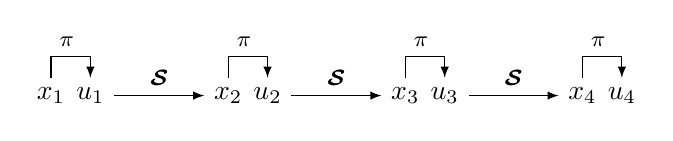
\begin{tikzpicture}
        \foreach \i in {4, ..., 1}{
                \node[name=xa\i] at (\i/4*9,0) {$x_\i$};
            }
        \foreach \i in {4, ..., 1}{
                \node[name=aa\i] at (\i/4*9+.5,0) {$u_{\i}$};
            }
        \foreach \i in {4, ..., 1}{
                \path[draw,->] (xa\i) -- +(0,.5)-| node[left,above,xshift = -0.3cm]{\footnotesize$\pi$} (aa\i);
            }
        \foreach \i in {3, ..., 1}{
                \pgfmathtruncatemacro{\j}{\i + 1}
                \path[draw,->] (aa\i)-- node[above]{\footnotesize$\S$} (xa\j);
            }
    \end{tikzpicture}
    \caption{Evolution of the closed-loop system.}
    \label{fig:closed_loop_system}
\end{figure}

\paragraph{Dataset}
Due to their complexity and opacity, such systems must often be treated as black boxes in their entirety, assuming only access to a finite amount, $N$, of system observations
\begin{equation}
    \data_N\colon \quad \{(x^i,a^i,x^i_+)\}_{i=1}^N,\label{eq:data}
\end{equation}
where every sampled transition from $x^i\in\X$ to a successor $x^i_+\in\X$ is generated as a realization
\begin{equation*}
    (x^i,a^i,x_+^i)\sim\int \delta_{f(x^i,a^i,w)}(dx_+^i)\,p_w(dw)\,\mathcal{U}_\X(dx^i)\,\mathcal{U}_\A(da^i),
\end{equation*}
with $\mathcal{U}_\X$ and $\mathcal{U}_\A$ uniform distributions on $\X$ and $\A$, respectively, and $\delta$ indicating the Dirac delta distribution capturing the system dynamics.

\begin{figure}[ht]
    \centering
    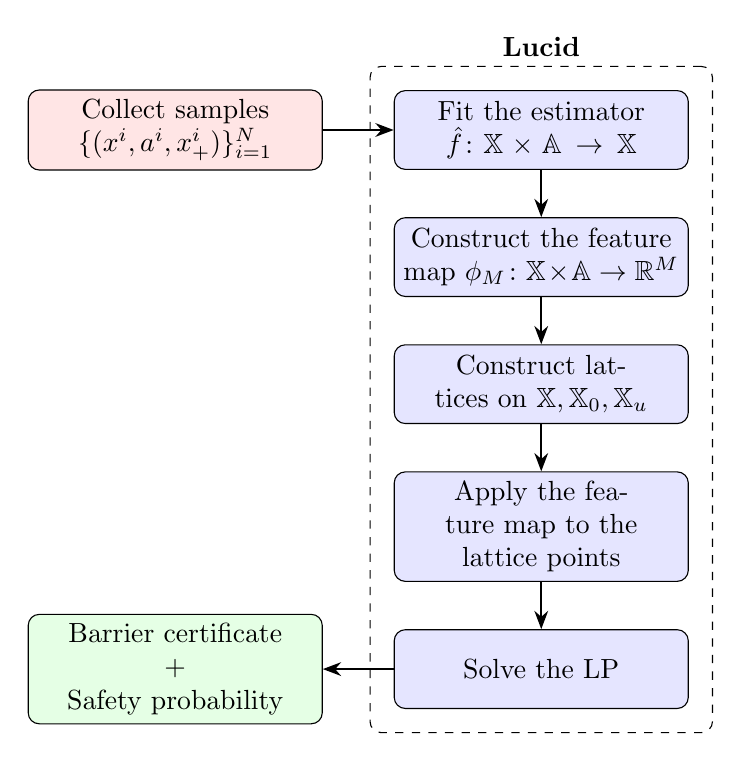
\begin{tikzpicture}[node distance=0.6cm and 0.9cm,
            input-block/.style={rectangle, draw, fill=red!10, text width=3.5cm, minimum height=1.0cm, align=center, rounded corners},
            output-block/.style={rectangle, draw, fill=green!10, text width=3.5cm, minimum height=1.0cm, align=center, rounded corners},
            block/.style={rectangle, draw, fill=blue!10, text width=3.5cm, minimum height=1.0cm, align=center, rounded corners},
            arrow/.style={thick,->,>=Stealth},
            tool/.style={rectangle, draw, fill=green!20, text width=2cm, minimum height=0.8cm, align=center, rounded corners},
            inv/.style={}
        ]

        % Input block
        \node[input-block] (input) {Collect samples $\{(x^i,a^i, x_+^i)\}_{i=1}^N$};

        % Lucid blocks
        \node[block, right=of input] (estimator) {Fit the estimator $\hat{f}\colon \X\times\A \to \X$};
        \node[block, below=of estimator] (feature) {Construct the feature map $\phi_M\colon \X\times\A \to \mathbb{R}^M$};
        \node[block, below=of feature] (lattice) {Construct lattices on $\X, \X_0, \X_u$};
        \node[block, below=of lattice] (apply-lattice) {Apply the feature map to the lattice points};
        \node[block, below=of apply-lattice] (optimizer) {Solve the LP};
        \node[draw, dashed, inner sep=0.3cm, rounded corners,
        fit=(estimator)(feature)(lattice)(apply-lattice)(optimizer), label=above:{\textbf{\lucid}}] {};

        % Output block
        \node[output-block, left=of optimizer] (output) {Barrier certificate\\+\\Safety probability};

        % Arrows
        \draw[arrow] (input) -- (estimator);
        \draw[arrow] (estimator) -- (feature);
        \draw[arrow] (feature) -- (lattice);
        \draw[arrow] (lattice) -- (apply-lattice);
        \draw[arrow] (apply-lattice) -- (optimizer);
        \draw[arrow] (optimizer) -- (output);

    \end{tikzpicture}
    \caption{Sequence of steps \lucid goes through to generate a barrier certificate.}
    \label{fig:steps}
\end{figure}


\paragraph{Safety Problem}
A question that often arises when designing a policy $\pi$ for a system $\S$, especially in engineering contexts, is if the closed-loop system $\S^\pi$ elicits safe behavior. That is, when starting from a domain $\X_{0}\subset\X$ under a policy $\pi$, the system $\S^\pi$ shall avoid unsafe regions $\X_U\subset\X$ (such as obstacles) for at least some predefined time horizon $T\in\N\cup\{\infty\}$.

%Such safety problems are tricky and even for the case where an explicit model \eqref{eq:model} is given, 
Certifying safety of a discrete-time stochastic system over an uncountable state space does not generally admit an analytical solution and is extremely challenging, especially for complex dynamics~\cite{abate2008probabilistic}.
Furthermore, for unbounded stochasticity $w_t\sim p_w$, there is generally no yes/no answer to safety, but a safety probability $P_{\text{safe}}(\S^\pi)\in[0,1)$. 
Note that given a policy $\pi$, for every initial state $x_0\in\X_0$ there is an associated safety probability. Our goal is to estimate a \emph{lower bound} on the infimum of such probabilities across all initial states in $\X_0$.
% Thus the goal is generally to estimate a \emph{lower bound} on the true safety probability $P_{\text{safe}}(\S^\pi)$. \textcolor{blue}{[Paolo] I think this needs clarification: given a policy $\pi$, for every initial state there is a safety probability. With Lucid we aim at computing a lower bound on the inf of such probabilities across all initial states. Did I understand correctly?}

\paragraph{Problem Statement}
Assuming access to a finite dataset $\data_N$ from the black-box system $\S$ in \eqref{eq:model}, quantify a certifiable lower bound on the probability of the black-box system $\S^\pi$ being safe with respect to a safety specification given by $(\X_0,\X_U,T)$.

\smallskip

Available sampling-based methods such as Monte Carlo simulation are unfit to solve this problem, as they compute guarantees for fixed initial conditions $x_0\in\X$.
\lucid provides a solution for continuous sets $\X_0$ by automating the steps in Figure~\ref{fig:steps}, outlined in the next sections.


\subsection{Control Barrier Certificates}\label{sec:cbc}
\glspl{cbc}\footnote[3]{\glspl{cbc} and discrete-time \glspl{cbf} \cite{cosner2023generative} are equivalent.} leverage the concept of set invariance to arrive at an abstraction-free numerical solution to finding a lower bound on $P_{\text{safe}}(\S^\pi)$. This has made them popular tools for safety verification and controller synthesis~\cite{prajna2006barrier}.

A non-negative function $\B\colon\X\rightarrow\R_{\geq 0}$ is a \gls{cbc} of a system $\S$ with reference to an unsafe set $\X_U$ if it satisfies
\begin{itemize}
    \item[(a)] $\forall x_0\in \X_0\colon\,\B(x_0)\leq\eta$;
    \item[(b)] $\forall x_U\in \X_U\colon\,\B(x_U)\geq\gamma$; and
    \item[(c)] $\forall x\in\X,\,\exists a\in\A\colon\,\E[\B(X_+) \mid X=x,\,A=a] -\B(x) \leq  c;$
\end{itemize}
for some constants $\gamma>\eta\geq0$ and $c\geq 0$. Here, upper case $X_+$, $X$, and $A$ denote the random variables underlying concrete realizations $(x_t,a_t,x_{t+1})$ elicited by $\S$.
%
Intuitively, if one can find a \gls{cbc} for a system $\S$, then, a lower bound on the probability of $\S$ being safe can be quantified based on the distance between the two level sets $\gamma$ and $\eta$~\cite{kushner1967stochastic}:
\begin{equation}
    P_{\text{safe}}(\S^\pi)\geq 1- \frac{\eta + cT}{\gamma},\label{eq:safety_prob_lb}
\end{equation}
where $T$ is the desired time horizon.
Notably, the system dynamics only enters the barrier conditions through the conditional expectation in (c), and a \gls{cbc} thus only depends on the \emph{expected} system behavior, with no need to consider its concrete stochastic law.

Whilst \eqref{eq:safety_prob_lb} can provide a robust assessment of a system's safety, in practice, the bound can be overly conservative and thus several improved variants of the original barrier constraints exist~\cite{mahathi2022kinductive}.
As these conditions in essence all rely on the computation of chance constraint with respect to the expected behavior of the system, they are basically interchangeable.

Although there exist model-\emph{based} efficient solutions to this problem for linear and control affine systems, this is generally a semi-infinite problem, demanding a data-driven solution. Furthermore, for the data-driven case, establishing constraint (c) rigorously without relying on impractical assumptions is extremely challenging.

\subsection{Data-Driven Dynamics Estimation via Conditional Mean Embeddings}\label{sec:dd_estimation_via_cme}
To reason about the expected value of a random variable, embedding the variable into a (higher dimensional) space and forming a data-driven estimate is a well-established concept in machine learning \cite{scholkopf2002learning,Steinwart2008SVM}.
Following the same reasoning, the \emph{kernel mean embedding} represents the projection of a probability measure into a \gls{rkhs} via a feature map $\phi$ associated with a positive definite kernel $k$~\cite{Smola2007EmbedDistrb,muandet2017kernel}.
For conditional probability distributions a similar concept exists: \glspl{cme} can be used to model the expected value of any \gls{rkhs} function $g\colon\X\rightarrow\R$ under a stochastic process such as $\S$~\cite{park2020measuretheoretic,muandet2017kernel}.
For the Gaussian kernel,
\begin{equation}
    k(x,x') := \sigma_f^2 \exp\left( -\tfrac{1}{2} (x-x')\T \Sigma\, (x-x') \right),\label{eq:gaussian_kernel}
\end{equation}
where $\Sigma:=\diag(\sigma_l)^{-2}$, with hyperparameters $\sigma_f,\sigma_l\in\R$, the associated RKHS encompasses all smooth functions $g$.
A data-driven estimate can then be obtained in closed form from a finite amount of data $\data_N$:
\begin{align}
    \begin{split}
         & \E[f(X_+)\mid X=x,\,A=a] \approx                                                  \\
        % \innerH{f}{\hat{\Psi}^N_{X^+|X}(x)}{\Hilbert_{k}} = 
         & \hspace{5em} k_{XA}^N(x,a)\T\left[ K_{XA}^N+N \lambda I_N\right]^{-1}\! f(X_+^N),
    \end{split}\label{eq:empiricalEstimate}
\end{align}
with column vector $k_{XA}^N(x,a):=[k((x^i,a^i),(x,a))]_{i=1}^N$, Gram matrix $K_{XA}^N:=[k((x^i,a^i),(x^j,a^j))]_{i,j=1}^N$, regularization factor $\lambda\geq0$, identity matrix $I_N$, and $f(X_+^N):=[f(x^i_+)]_{i=1}^N$.
The empirical estimator in \eqref{eq:empiricalEstimate} converges in expectation to the true \gls{cme} for $N\rightarrow\infty$~\cite{park2020measuretheoretic}.

It is common practice to robustify empirical estimates such as \eqref{eq:empiricalEstimate} to out-of-sample behavior by constructing an \gls{rkhs} ambiguity set centered at the empirical \gls{cme}. The result is a distributionally robust estimator with an adjustable robustness radius. The details are omitted here for brevity, but the interested reader is referred to the works by \citet{kuhn2025distributionally} and \citet{li2022optimal}.


\subsection{Data-Driven Spectral Barriers}\label{sec:ddbarriers}
Based on the data-driven estimator in \eqref{eq:empiricalEstimate}, the problem of computing \glspl{cbc} using data can be formulated as a nonconvex semi-infinite program, which for general classes of systems and barriers is extremely difficult to solve.
To arrive at a tractable solution, \lucid conducts two additional steps:
\paragraph{1. Spectral Abstraction} Inspired by the popular random Fourier features approach by \citet{rahimi2007random}, the Gaussian kernel \eqref{eq:gaussian_kernel} admits a Fourier expansion
\begin{align}
    k(x, x') \equiv \sigma_f^2 \int_{\R^{n}}\!\! \mathcal{N}(d\omega\mid0,\Sigma)\; e^{\mathbf{i}\omega\T (P(x)-P(x'))},\label{eq:sqexp_kernel_fourier}
\end{align}
with the zero-mean Gaussian distribution $\smash{\mathcal{N}(d\omega\mid0,\Sigma)}$ with covariance $\Sigma$, the imaginary unit $\mathbf{i}:=\smash{\sqrt{-1}}$, and where the projection $x \mapsto P(x)$ maps the domain $\X$ into the unit hypercube $[0,1]^{n}$.
Partitioning the space of spatial frequencies $\omega\in\R^n$ into a set of discrete frequency bands (see Figure~\ref{fig:spectral_barrier}) yields a spectral abstraction of the associated \gls{rkhs}, i.e., characterizing learnable functions $\B$ in the form of Fourier series.
By truncating the series to a finite number, $M$, of fixed frequency bands $\omega_j\in\R^{n}$, $j\in\{0,\ldots,M\}$, the resulting barriers are of the form
\begin{align*}
    \B(x) = \alpha_0 +\sum_{i=1}^{M} \alpha_i \cos\left(\omega_i\T P(x)\right) + \beta_i \sin\left(\omega_i\T P(x)\right).%\label{eq:blackbox:representer_form_spectral}
\end{align*}
Notably, $\B$ admits the linear form $\B(x)=\phi_M(x)\T b$, with a truncated Fourier feature map $\phi_M\colon\X\rightarrow\R^{2M+1}$, parametrized by learnable spectral amplitudes
\begin{figure}
    \centering
    \includegraphics[width=0.9\linewidth]{fourier_series.pdf}
    \caption{Spectral barrier certificate $\B(x)=\phi_M(x)\T b$.}
    \vspace{-0.3cm}
    \label{fig:spectral_barrier}
\end{figure}
\begin{align*}
    b\!=\!\begin{bmatrix}
              \frac{\alpha_0}{\sigma_f^2\w_0^2}\!\! & \frac{\alpha_1}{2\sigma_f^2\w_1^2}\!\!\! & \frac{\beta_1}{2\sigma_f^2\w_1^2}\!\!\! & \ldots\!\!\! & \frac{\alpha_{M}}{2\sigma_f^2\w_{M}^2}\!\!\! & \frac{\beta_{M}}{2\sigma_f^2\w_{M}^2}
          \end{bmatrix}\T\!\!\!\!\in\R^{2M+1}\!\!,
\end{align*}
where the weights $\w_0,\ldots,\w_{M}\in\R_{\geq 0}$ associated with each frequency band are determined efficiently from the kernel's Gaussian spectral measure via the multivariate CDF (see Figure~\ref{fig:spectral_measure_abstraction}).
The \gls{cme}-based estimator \eqref{eq:empiricalEstimate} is approximated in the same finite basis via $H\in\R^{(2M+1)\times (2M+1)}$ such that
\begin{equation*}
    k_{XA}^N(x,a)\T\left[ K_{XA}^N+N \lambda I_N\right]^{-1}\! \Phi_{M,+}^N
    \approx
    \varphi_M(x,a)\T H,
\end{equation*}
where $\Phi_{M,+}^N:=[\phi_M(x_+^i)\T]_{i=1}^N$, $\varphi_M(x,a)\colon\X\times\A\rightarrow\smash{\R^{2M+1}}$ a feature map augmenting $\phi_M(x)$, and
with an approximation error decreasing exponentially with $M$~\cite{rahimi2007random}.
This reduces the barrier synthesis problem
% This simplifies the barrier problem 
to a semi-infinite linear program, with barrier conditions linear in $b$:
\begin{itemize}
    \item[(a)] $\forall x_0\in \X_0\colon\,\phi_M(x_0)\T b\leq\eta$;
    \item[(b)] $\forall x_U\in \X_U\colon\,\phi_M(x_U)\T b\geq\gamma$; and
    \item[(c)] $\forall x\in\X,\,\exists a\in\A\colon\,\varphi_M(x,a)\T (Hb -b) \leq  c.$
\end{itemize}
For the case where $a$ is provided by a given fixed policy $\pi$, $\varphi_M(x,a)$ reduces to $\phi_M(x)$.
% \OS{Importantly, the closed-form estimator in \eqref{eq:empiricalEstimate} does not depend on the choice of features and only through the spectral abstraction is the feature map introduced directly.}
\begin{figure}
    \centering
    % GAUSSIANs: 68-95-99 rule
    \begin{tikzpicture}
        \def\N{50} % number of sample points
        \def\B{0};
        \def\Bs{3.0};
        \def\var{1.3}
        \def\xmax{\B+3.5*\Bs};
        \def\ymin{{-0.1*gauss(\B,\B,\Bs)}};
        \def\h{0.08*gauss(\B,\B,\Bs)};

        \begin{axis}[every axis plot post/.append style={
            mark=none,domain={-(\xmax)}:{1.0*\xmax},samples=\N,smooth},
            xmin={-(\xmax)}, xmax=\xmax,
            axis/.style={>=latex},
            ymin=\ymin, ymax={1.1*gauss(\B,\B,\Bs)},
            axis lines=middle,
            axis line style=thick,
            enlarge x limits, % extend the axes a bit
            ticks=none,
            xlabel=$\omega$,
            every axis x label/.style={at={(current axis.right of origin)},anchor=north},
            width=1.1\linewidth, height=0.55*\linewidth,
            y=700pt,
            clip=false,
            axis line style={-latex}
            ]

            % PLOTS
            \addplot[accent,thick,name path=B] {gauss(x,\B,\var*\Bs)};

            % FILL
            \path[name path=xaxis]
            (\B-\pgfkeysvalueof{/pgfplots/xmax},0) -- (\B+\pgfkeysvalueof{/pgfplots/xmax},0); %\pgfkeysvalueof{/pgfplots/xmin}
            \addplot[accent!3.75] fill between[of=xaxis and B, soft clip={domain={\B-3.5*\Bs}:{\B+3.5*\Bs}}];
            \addplot[accent!7.5] fill between[of=xaxis and B, soft clip={domain={\B-2.5*\Bs}:{\B+2.5*\Bs}}];
            \addplot[accent!15] fill between[of=xaxis and B, soft clip={domain={\B-1.5*\Bs}:{\B+1.5*\Bs}}];
            \addplot[accent!30] fill between[of=xaxis and B, soft clip={domain={\B-.5*\Bs}:{\B+.5*\Bs}}];

            % LINES
            \addplot[black,dashdotted,thin]
            coordinates {({\B-3*\Bs},{20*gauss(\B-3*\Bs,\B,\Bs)}) ({\B-3*\Bs},{-\h})}
            node[below=-3pt,scale=1.0] {\strut$\omega_3$};
            \addplot[black,dashdotted,thin]
            coordinates {({\B-2*\Bs},{4*gauss(\B-2*\Bs,\B,\Bs)}) ({\B-2*\Bs},{-\h})}
            node[below=-3pt,scale=1.0] {\strut$\omega_2$};
            \addplot[black,dashdotted,thin]
            coordinates {({\B-1*\Bs},{1.3*gauss(\B-\Bs,\B,\Bs)}) ({\B-1*\Bs},{-\h})}
            node[below=-3pt,scale=1.0] at ({\B-\Bs},{-\h}) {\strut$\omega_1$};
            \addplot[black,dashdotted,thin]
            coordinates {(\B,{1.05*gauss(\B,\B,\Bs)}) (\B,{-\h})}
            node[below=-3pt,scale=1.0] {\strut$\omega_0$};
            \node[scale=1.0] (w0)
            at ({\B+.5*\Bs},{.125}) {$\w_0^2$};
            \node (b0) at ({\B+.25*\Bs},{.08}) {};
            \draw[->] (w0) to (b0.center);
            % \addplot[white,dashed,thin]
            % coordinates {({\B+.5*\Bs},{gauss(\B+.5*\Bs,\B,\Bs)}) ({\B+.5*\Bs},0)};
            \addplot[black,dashdotted,thin]
            coordinates {({\B+1*\Bs},{1.3*gauss(\B+\Bs,\B,\Bs)}) ({\B+1*\Bs},{-\h})}
            node[below=-3pt,scale=1.0] at ({\B+\Bs},{-\h}) {\strut$\omega_1$};
            \node[scale=1.0] (w1)
            at ({\B+1.5*\Bs},{.085}) {$\frac{\w_1^2}{2}$};
            \node (b1) at ({\B+1.25*\Bs},{.04}) {};
            \draw[->] (w1) to (b1.center);
            \addplot[black,dashdotted,thin]
            coordinates {({\B+2*\Bs},{4*gauss(\B+2*\Bs,\B,\Bs)}) ({\B+2*\Bs},{-\h})}
            node[below=-3pt,scale=1.0] at ({\B+2*\Bs},{-\h}) {\strut$\omega_2$};
            \node[scale=1.0] (w2)
            at ({\B+2.5*\Bs},{.055}) {$\frac{\w_2^2}{2}$};
            \node (b2) at ({\B+2.25*\Bs},{.01}) {};
            \draw[->] (w2) to (b2.center);
            \addplot[black,dashdotted,thin]
            coordinates {({\B+3*\Bs},{20*gauss(\B+3*\Bs,\B,\Bs)}) ({\B+3*\Bs},{-\h})}
            node[below=-3pt,scale=1.0] at ({\B+3*\Bs},{-\h}) {\strut$\omega_3$};
            \node[scale=1.0] (w3)
            at ({\B+3.5*\Bs},{.046}) {$\frac{\w_3^2}{2}$};
            \node (b3) at ({\B+3.25*\Bs},{.001}) {};
            \draw[->] (w3) to (b3.center);

            % Hyperparameters
            \addplot[<->,accent]
            coordinates {({\B-2*\var*\Bs},{gauss(\B+2*\var*\Bs,\B,\var*\Bs)}) ({\B+2*\var*\Bs},{gauss(\B+2*\var*\Bs,\B,\var*\Bs)})};
            \node[accent,fill=accent!30,inner xsep=3,inner ysep=2,scale=.8] at (\B,{gauss(\B+2*\var*\Bs,\B,\var*\Bs)}) {$\pm 2\sigma_l$};
            \addplot[<->,accent]
            coordinates {({\B-3*\var*\Bs},{gauss(0,0,\var*\Bs)}) ({\B-3*\var*\Bs},{0})};
            \addplot[dashed,thin,accent]
            coordinates {({\B-3*\var*\Bs},{gauss(0,0,\var*\Bs)}) ({0},{gauss(0,0,\var*\Bs)})};
            \node[accent,fill=white,inner xsep=3,inner ysep=2,scale=.8] at (\B-3*\var*\Bs,{.5*gauss(0,0,\var*\Bs)}) {$\sigma_f^2$};

        \end{axis}
    \end{tikzpicture}
    % \includegraphics[width=\linewidth]{figures/spectral_measure_abstraction.png}
    \caption{Abstraction of a 1-dim. Gaussian spectral measure of the Gaussian kernel, shown in \eqref{eq:sqexp_kernel_fourier}.}
    \vspace{-0.5cm}
    \label{fig:spectral_measure_abstraction}
\end{figure}
% Naturally, barriers of the form \eqref{eq:blackbox:representer_form_spectral} will be referred to as \emph{Fourier control barrier certificates}.

\paragraph{2. Finite-Constraint Relaxation} To obtain a program with \emph{finitely} many constraints, trigonometric bounding results \cite{pfister2018bounding} are used to obtain a relaxed linear program by sampling spatial lattices on $\X$, $\X_0$, and $\X_U$.
For example, to enforce barrier constraint (a) in Section~\ref{sec:cbc}, it suffices to construct a lattice $\{x_0^i\}_{i=1}^{N_0}\subset\X_0$ and impose the constraints $b\T\phi_M(x_0^i)\leq\eta$ for $i=1,\ldots,N_0$.
Selecting lattices with a sampling density meeting the Nyquist-Shannon sampling theorem with respect to the highest frequency $\omega_M$ appearing in the barrier and truncated estimator, the relaxation retains all guarantees.
As a result, the semi-infinite problem is relaxed to a finitely-constrained \gls{lp}, provided in full in the supplementary material.
Recall that given an appropriate robustness radius, the barriers produced by \lucid based on data $\data_N$ are statistically correct with respect to the unknown true system $\S$, and a lower bound for the safety probability is computed according to \eqref{eq:safety_prob_lb}.
%\Sadegh{Just to double check: we are not making the third inequality more conservative related to CME.} \OS{Not currently implemented.}

\section{Tool Structure and Functionalities}
\label{sec:tool}
\lucid implements the previously outlined functionality, written in C++ and designed to be used as a library or standalone executable.
The choice of a low level language gives us plenty of freedom and fine-grained control over the execution of the software.
We expose a set of interfaces allowing users to highly customize the verification process.
A high-level visualization of \lucid's architecture is illustrated in Figure~\ref{fig:architecture}, while a more technical description can be found in the online documentation at
\begin{center}
    \url{https://lucidtoolsource.gitlab.io/lucid/}.
\end{center}
% \lucid's source code is hosted at \url{https://gitlab.com/lucidtoolsource/lucid}.

We also provide a Python wrapper, called \pylucid, to facilitate the integration of the tool into existing workflows and effortlessly leverage well-established libraries such as NumPy~\cite{numpy} and SciPy~\cite{scipy}.
Moreover, \pylucid can be extensively configured in a variety of ways (e.g., Python scripts, YAML files, GUI), making it the recommended way to operate \lucid.
Hence, for the rest of the paper, we will focus on \pylucid when describing the user interfaces.
Further information about \pylucid are deferred to the supplementary material.


\paragraph{Configuration}
% The system and the specification \lucid will check against shall be provided as a configuration to the program.
To certify safety of a system, \lucid accepts a configuration comprising data from the system and the safety specification.
We suggest defining it as a \yaml or equivalent \json file.
%\footnote[4]{The Json schema for \yaml and \json files can be found at \url{https://lucidtoolsource.gitlab.io/lucid/configuration_schema.json}}
% \OS{I would personally avoid the word "scenario", as it could be misunderstood with an actual run of the system.}
If more flexibility is needed, a Python script generating a configuration can be used instead,
with the only requirement being that it must contain a function named \lstinline|scenario_config| returning a \texttt{Configuration} object.
Regardless of their format, configuration files can be loaded with the command \lstinline|pylucid <config file>| to start the tool's verification pipeline.
The same configuration values can also be given directly as command line arguments.
\pylucid also provides a browser-based \gls{gui} to aid in the configuration and execution of the tool.

In its current form, \lucid implements all the functionalities needed to certify safety of a closed-loop system with a given control policy $\pi$.
Thus the action $a$ in the previous section is replaced with the policy $\pi(x)$.
Future releases will expand this core functionality to
safe controller synthesis as well.
Due to its modular architecture, \lucid can be easily extended in multiple directions, as outlined in Section~\ref{sec:conclusion_and_future_extensions}.

\subsection{Configuring and Running the Tool}
% \todo{Map the theoretical modules from Section~\ref{sec:theory} to components/modules of the code.}

\lucid is built with a modular architecture where each component is responsible for a specific task in the certification process.
Moreover, since they extend from a common interface, they can be easily replaced or extended.
An overview of the core components and how they interact is shown in Figure~\ref{fig:architecture}.
Classes and interfaces available in \pylucid are written in \texttt{monospace font}.

To make the explanation more intuitive, we will use as a running example the one-dimensional linear system
\begin{equation}
    \label{eq:linear-system}
    \S\colon%\begin{bmatrix}
    \quad
    {x}_{t+1}
    %\end{bmatrix}
    = %\begin{bmatrix}
    0.5
        %\end{bmatrix}
        %\begin{bmatrix}
        {x}_{t}
    %\end{bmatrix} 
    + w_t,
    \quad w_t \sim \mathcal{N}(\cdotx | 0, 0.01),
\end{equation}
% where $x_t$ is the state at time $t$ and $w_t$ is Gaussian noise.
% Given the
with
state space $\X = [-1, 1]$, initial set $\X_0 = [-0.5, 0.5]$, and unsafe regions $\X_U = [-1, -0.9] \cup [0.9, 1]$.
While going over each component of \lucid, we will show how they can be configured within a \yaml configuration file to capture the system~\eqref{eq:linear-system} and its safety specification.

\paragraph{Dataset}
% \todo{Should this be considered a component? It is more about the data loader} \Sadegh{This is good to have as a separate component.}
Due to its data-driven nature, all that \lucid needs to operate, is a set of sampled transitions $\data_N$ from the system, as shown in \eqref{eq:data}, and the safety specification itself.
% Data can be obtained by defining a function that takes as input the current state and control input and returns the next state, adding i.i.d. noise sampled from an appropriate distribution, or it may be collected from an external simulator or real-world system.
The samples can be specified directly in the configuration file, divided into $x^1,\ldots,x^N$ and $x^1_+,\ldots,x^N_+$:
\begin{lstlisting}[language=yaml,backgroundcolor=\color{ipython_bg}]
x_samples: [[5.930e-01], ..., [-1.937e-01]]
xp_samples: [[3.015e-01], ..., [-1.018e-01]]
\end{lstlisting}
Alternatively, the samples can either be generated by the Python configuration script, or be stored in a separate file.
% Refer to the documentation for more details.
\begin{comment}
\begin{lstlisting}[language=iPython]
    def scenario_config():
    # ...
    # Sampling
    f = lambda x: x / 2
    c.x_samples = c.X_bounds.sample(1000)
    c.xp_samples = f(c.x_samples) + np.random.normal(scale=0.01)
    # ...
    return c
\end{lstlisting}
\end{comment}

\begin{figure}
    \centering
    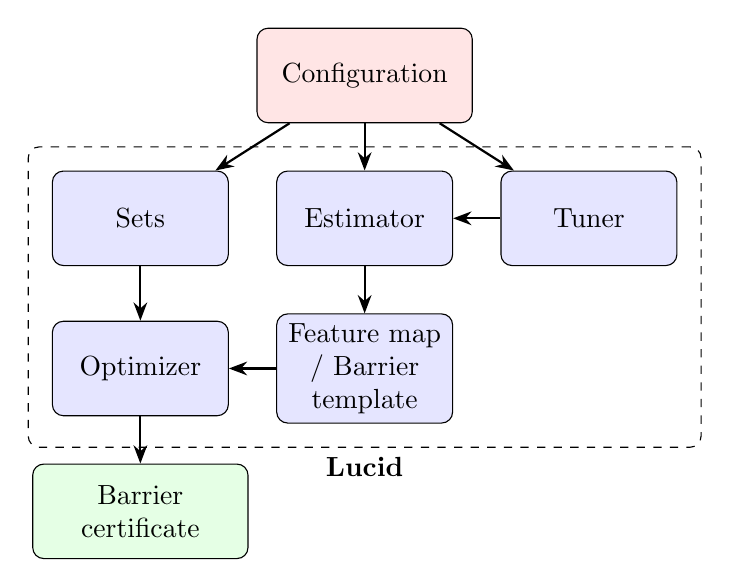
\begin{tikzpicture}[node distance=0.6cm and 0.6cm,
            input-block/.style={rectangle, draw, fill=red!10, text width=2.5cm, minimum height=1.2cm, align=center, rounded corners},
            output-block/.style={rectangle, draw, fill=green!10, text width=2.5cm, minimum height=1.2cm, align=center, rounded corners},
            block/.style={rectangle, draw, fill=blue!10, text width=2.0cm, minimum height=1.2cm, align=center, rounded corners},
            arrow/.style={thick,->,>=Stealth},
            tool/.style={rectangle, draw, fill=magenta!10, text width=3cm, minimum height=0.8cm, align=center, rounded corners},
            inv/.style={}
        ]

        % Input block
        \node[input-block] (input) {Configuration};

        % Lucid blocks
        \node[block, below=of input] (estimator) {Estimator};
        \node[block, right=of estimator] (tuner) {Tuner};
        \node[block, left=of estimator] (sets) {Sets};
        \node[block, below=of estimator] (feature) {Feature map / Barrier template};
        \node[block, left=of feature] (optimizer) {Optimizer};
        % \node[block, below=of optimizer] (verifier) {Verifier};
        \node[draw, dashed, inner sep=0.3cm, rounded corners,
        % fit=(estimator)(feature)(optimizer)(verifier), label=above:{\textbf{Lucid}}] {};
        fit=(estimator)(feature)(optimizer)(sets)(tuner), label=below:{\textbf{Lucid}}] {};

        % Output block
        % \node[output-block, left=of verifier] (output) {Barrier certificate};
        \node[output-block, below=of optimizer] (output) {Barrier certificate};

        % Smt solvers
        % \node[inv, below=2.5cm of verifier.north, anchor=north] (smtInv) {};
        % \node[tool, left=0.3cm of smtInv] (dreal) {dReal};
        % \node[tool, right=0.3cm of smtInv] (cvc5) {CVC5};
        % \node[draw, dashed, inner sep=0.3cm, rounded corners,
        % fit=(dreal)(cvc5), label=left:{\textbf{SMT Solver}}] {};

        % Arrows
        \draw[arrow] (input) -- (estimator);
        \draw[arrow] (input) -- (tuner);
        \draw[arrow] (input) -- (sets);
        \draw[arrow] (sets) -- (optimizer);
        \draw[arrow] (tuner) -- (estimator);
        \draw[arrow] (estimator) -- (feature);
        \draw[arrow] (feature) -- (optimizer);
        % \draw[arrow] (optimizer) -- (verifier);
        % \draw[arrow] (verifier) -- (output);
        \draw[arrow] (optimizer) -- (output);

        % \draw[arrow] (cvc5.north) -- (verifier.south);
        % \draw[arrow] (dreal.north) -- (verifier.south);

    \end{tikzpicture}
    \caption{General architecture of Lucid, highlighting its core components and their connections.}
    \label{fig:architecture}
\end{figure}


\paragraph{\Circled{1}~Safety Specification}
\lucid understands sets $\X,\X_0,\X_U$ specified as \texttt{RectSet}, \texttt{SphereSet}, or \texttt{Multiset} objects (collections of sets from the first two categories).
% Sets are mainly used to indicate the bounds of the whole state space $\X$, the initial set $\X_0$ and the unsafe set $\X_U$ in the context of defining the safety specification to verify.
They can be included in the configuration as shown below:
\begin{lstlisting}[language=yaml,backgroundcolor=\color{ipython_bg}]
X_bounds: "RectSet([-1], [1])"
X_init: "RectSet([-0.5], [0.5])"
X_unsafe: 
  - "RectSet([-1], [-0.9])"
  - "RectSet([0.9], [1])"
\end{lstlisting}
% \OS{So is the \lstinline{X_unsafe} here a Multiset?}

\paragraph{\mbox{\Circled{2}\hspace{.4em}Estimator}}
The core of \lucid is its \estimator, namely the \texttt{KernelRidgeRegressor}, which uses the \texttt{GaussianKernel} to learn the underlying system dynamics by estimating the \gls{cme} from the samples.
Its predictions of the expected next state $x_+$ are used
% of all the lattice points we need from $\X$, necessary 
to determine the constraints for the \gls{cbc} \gls{lp}.
% The \hp of the \texttt{KernelRidgeRegressor} can be set explicitly in the configuration file:
% We provide the \hp values for the kernel, namely the bandwidth $\sigma_f = 1$, the length scale $\sigma_l = 1.75555556$, values obtained from a previous tuning process, 
% and the regularization constant $\lambda = 0.00001$.
The setup is configured as follows:
\begin{lstlisting}[language=yaml,backgroundcolor=\color{ipython_bg}]
kernel: "GaussianKernel"
estimator: "KernelRidgeRegressor"
\end{lstlisting}


\paragraph{\Circled{3}~Tuner}
Being parameter-free approaches, kernel methods do not require the expensive learning processes of other machine learning methods, such as neural networks.
However, they still depend on a number of \hp, such as the kernel bandwidth $\sigma_f$, the lengthscale $\sigma_l$, and the regularization constant $\lambda$ (see \eqref{eq:gaussian_kernel}--\eqref{eq:empiricalEstimate}).
Changes in their values can have a significant impact on the \estimator's efficiency and accuracy.
The process of finding good values for these \hp is known as \emph{hyperparameter tuning}, with the optimal parameters being problem dependent.
\lucid provides a set of utilities, which specialize the \texttt{Tuner} interface, to aid in this task:
\begin{itemize}
    \item \texttt{MedianHeuristicTuner} uses the \emph{median heuristic} \cite{garreau2018largesampleanalysismedian} to produce rule-of-thumb-type estimates for the \hp $\sigma_f$ and $\sigma_l$ of, e.g., the Gaussian kernel \eqref{eq:gaussian_kernel}, via closed-form expressions.
          It can be useful as a starting point for subsequent improvements.
    \item \texttt{LbfgsTuner} finds the \hp that maximize the \emph{log marginal likelihood}~\cite{rasmussen2006gaussian}, defined as
          \begin{equation*}
              \begin{split}
                   & \log p(X^+_N | X_N,\theta) =  - \frac{1}{2}X^+_N{}\T (K_{X}^N + N\lambda I_N)^{-1} X^+_N \\
                   & \hspace{40pt} -\frac{1}{2}\log |K_{X}^N + N\lambda I_N| - \frac{N}{2}\log(2\pi),
              \end{split}
          \end{equation*}
          where $\theta:=(\sigma_f,\sigma_l,\lambda)$ is the hyperparameter being optimized.
          We use the L-BFGS or L-BFGS-B quasi-Newton optimization algorithms~\cite{book:nonlinear-programming},
          implemented in the \texttt{LBFGS++} library~\cite{LBFGSpp}.
          %          \footnote{https://github.com/yixuan/LBFGSpp}
    \item \texttt{GridSearchTuner} implements the grid search method, exploring the space of possible \hp values to find the one that maximizes the \estimator's $R^2$ score, defined as $$R^2 = 1 - \textstyle\left(\sum_{i=1}^M (y_i - \hat{y}_i)^2/\sum_{i=1}^M (y_i - \bar{y})^2\right),$$ with $\hat{y}_i$ and $\bar{y}:=(\sum_{i=1}^N y_i)/N$ being the $i^{\text{th}}$ predicted and mean observed outputs, respectively.
\end{itemize}
Tuners open a wide range of possibilities to the user.
We recommend using them within a Python script generating a configuration to automate the tuning process before finalizing the \estimator's hyperparameter values:
\begin{lstlisting}[language=iPython,style=nonumbers]
def scenario_config(c: Configuration):
    t = LbfgsTuner(lb=[1e-5], ub=[1e5])
    c.estimator = KernelRidgeRegressor()
    c.estimator.fit(c.x_samples, c.xp_samples, tuner=t)
    return c
\end{lstlisting}
In this example, we set the \hp explicitly:
\begin{lstlisting}[language=yaml,backgroundcolor=\color{ipython_bg}]
sigma_f: 15
sigma_l: [1.2]
lambda: 1.0e-5
\end{lstlisting}

\begin{comment}
A cheap starting point when working with a Gaussian kernel as in~\eqref{eq:gaussian_kernel} is to use the \emph{median heuristic} \cite{garreau2018largesampleanalysismedian}, implemented in the \texttt{MedianHeuristicTuner}.
\OS{We can cut the following to save space. This is standard knowledge:}
{\color{gray}
    We choose $\sigma_l^2$ to be the median of the squared distances between all pairs of points in the training set, i.e.,
    \begin{equation}
        \sigma_l^2 = \mathrm{median}_{1 \leq i < j \leq N}\left(\|\hat{x}_i-\hat{x}_j\|^2\right),
    \end{equation}
    where $\hat{x}_1,\ldots,\hat{x}_N$ are the $N$ training samples.
    If $N(N-1)/2$ is even, the median is the average of the two middle values in the sorted list of distances.}
The \texttt{GridSearchTuner}, on the other hand, implements the grid search method, exploring the space of possible \hp values to find the one that yields the best \estimator $R^2$ score,
defined as $R^2 = 1 - \frac{\sum_{i=1}^n (y_i - \hat{y}_i)^2}{\sum_{i=1}^n (y_i - \bar{y})^2}$.
This approach is simple to implement and can be very effective for small problems, but it can become computationally expensive for larger ones.
Borrowing a technique from Gaussian processes, we can also optimize the \hp to maximize the \emph{log marginal likelihood}, defined as
\begin{equation}
    \begin{split}
         & \log p(X^+_N | X_N,\theta) =  - \frac{1}{2}X^+_N{}\T (K_{X}^N + N\lambda I_N)^{-1} X^+_N \\
         & \hspace{40pt} -\frac{1}{2}\log |K_{X}^N + N\lambda I_N| - \frac{N}{2}\log(2\pi),
    \end{split}
\end{equation}
where $\theta:=(\sigma_f,\sigma_l, M)$ \OS{Which are implemented?} contains all learnable hyperparameters (of the kernel).
To do so, the \texttt{LbfgsTuner} uses the L-BFGS or L-BFGS-B quasi-Newton optimization algorithms~\cite{book:nonlinear-programming},
implemented in the \texttt{LBFGS++} library\footnote{https://github.com/yixuan/LBFGSpp}.
\end{comment}

\paragraph{\Circled{4}~Feature Map}
We exploit the spectral kernel expansion in \eqref{eq:sqexp_kernel_fourier} by building an explicit approximated feature map, composed of a linear sum of trigonometric functions with increasing frequencies (see Figure~\ref{fig:spectral_barrier}).
The underlying kernel expansion, visualized in Figure~\ref{fig:spectral_measure_abstraction}, can be controlled to trade-off efficiency and accuracy/conserativeness.
% The full expansion of the kernel would need a sum of infinitely many terms with diminishing impact on the overall result, which we truncate arbitrarily short, a decision based on the tradeoff we are looking for between efficiency and accuracy.
After being defined with the same \hp $(\sigma_f,\sigma_l)$ that characterize the \texttt{KernelRidgeRegressor}, the function can be used to map any point from $\X$ to the \gls{rkhs} associated with the kernel.
\lucid currently implements three different ways for partitioning the spectral measure in Figure~\ref{fig:spectral_measure_abstraction}:
\begin{itemize}
    \item \texttt{LinearTruncatedFourierFeatureMap} defines equally spaced frequency bands on the interval $[-3\sigma_l,3\sigma_l]$, capturing 99.73\% of the spectral measure. This partitioning is shown in Figure~\ref{fig:spectral_measure_abstraction}.
    \item \texttt{LogTruncatedFourierFeatureMap} defines logarithmically spaced frequency bands on the interval $[-3\sigma_l,3\sigma_l]$, with each frequency band carrying an equal share of the spectral measure.
    \item \texttt{ConstantTruncatedFourierFeatureMap} defines frequency bands with a fixed size.
\end{itemize}
Different feature map implementations may yield different results.
In our example, we truncate the Fourier expansion to $5$ frequency bands, including the constant term, and use $704$ lattice points to build the constraints of the optimization problem, to avoid it being too conservative.
\begin{lstlisting}[language=yaml,backgroundcolor=\color{ipython_bg}]
feature_map: 
    "LinearTruncatedFourierFeatureMap"
num_frequencies: 5
num_oversample: 704
\end{lstlisting}

\paragraph{\Circled{5} Solver}
% \todo{Barriers should probably be an explicit class in \lucid that hides the optimization implementation}
Based on the components discussed above, \lucid generates and solves a finite-constraint \gls{lp} as outlined in Section~\ref{sec:ddbarriers}.
% If successful, the output is a \glspl{cbc} and a quantified lower bound on the true safety probability $P_{safe}(\S^\pi)$.
%
% When verifying the safety of a system, \lucid will search for a \gls{cbc} $\B$ that satisfies the conditions in Definition~\ref{def:cbc}.
If successful, \lucid returns a \gls{cbc}, a quantified lower bound on the true safety probability $P_{safe}(\S^\pi)$, as well as the corresponding constants $\eta$, $\gamma$, and $c$.
% More precisely, we follow the steps outlined in Figure~\ref{fig:steps}.

Generating the \gls{lp}, specifically choosing an appropriate lattice density, involves trading off efficiency versus conservativeness, with any sampling density beyond the Nyquist frequency yielding a valid relaxation.
In the benchmarks in Section~\ref{sec:experiments}, we showcase the relation numerically.
% (see Section~\ref{sec:ddbarriers})
%
% While the theory gives us a precise indication on how to construct the \gls{lp} which yields a correct-by-design solution, in practice the constraints may be too conservative to find a valid solution.
% To mitigate this, the user can either increase the number of lattice points $Q$, worsening the computational efficiency,
% or adjust the coefficient $C_{\hat{N}}$, improving performance at the cost of loosening the guarantees.
For solving the \gls{lp}, \lucid can interface with different linear optimizers: \gurobi, \alglib, or \highs. Here, we use \gurobi:
\begin{lstlisting}[language=yaml,backgroundcolor=\color{ipython_bg}]
optimiser: "GurobiOptimiser"
\end{lstlisting}

\paragraph{Running the Tool}
We have configured all the components needed to run \lucid.
Putting it all together in a single configuration file \texttt{config.yaml} we can run the tool with the command \lstinline|pylucid config.yaml --plot|.
\lucid will parse the configuration, synthesize a barrier certificate and plot the result.
For the running example, we obtain the barrier certificate shown in Figure~\ref{fig:example} for a time horizon of $T = 15$ certifying safety of the system in \eqref{eq:linear-system} with a probability of at least $95.12\%$ ($\eta = 0.03, \gamma=1.0, c = 0.001$). %\|B\| = 1.72

\begin{figure}
    \centering
    \begin{adjustbox}{max width=\columnwidth}
        %% Creator: Matplotlib, PGF backend
%%
%% To include the figure in your LaTeX document, write
%%   \input{<filename>.pgf}
%%
%% Make sure the required packages are loaded in your preamble
%%   \usepackage{pgf}
%%
%% Also ensure that all the required font packages are loaded; for instance,
%% the lmodern package is sometimes necessary when using math font.
%%   \usepackage{lmodern}
%%
%% Figures using additional raster images can only be included by \input if
%% they are in the same directory as the main LaTeX file. For loading figures
%% from other directories you can use the `import` package
%%   \usepackage{import}
%%
%% and then include the figures with
%%   \import{<path to file>}{<filename>.pgf}
%%
%% Matplotlib used the following preamble
%%   \def\mathdefault#1{#1}
%%   \everymath=\expandafter{\the\everymath\displaystyle}
%%   \IfFileExists{scrextend.sty}{
%%     \usepackage[fontsize=10.000000pt]{scrextend}
%%   }{
%%     \renewcommand{\normalsize}{\fontsize{10.000000}{12.000000}\selectfont}
%%     \normalsize
%%   }
%%   
%%   \ifdefined\pdftexversion\else  % non-pdftex case.
%%     \usepackage{fontspec}
%%     \setmainfont{DejaVuSerif.ttf}[Path=\detokenize{/home/campus.ncl.ac.uk/c3054737/miniconda3/envs/pylucid/lib/python3.11/site-packages/matplotlib/mpl-data/fonts/ttf/}]
%%     \setsansfont{DejaVuSans.ttf}[Path=\detokenize{/home/campus.ncl.ac.uk/c3054737/miniconda3/envs/pylucid/lib/python3.11/site-packages/matplotlib/mpl-data/fonts/ttf/}]
%%     \setmonofont{DejaVuSansMono.ttf}[Path=\detokenize{/home/campus.ncl.ac.uk/c3054737/miniconda3/envs/pylucid/lib/python3.11/site-packages/matplotlib/mpl-data/fonts/ttf/}]
%%   \fi
%%   \makeatletter\@ifpackageloaded{underscore}{}{\usepackage[strings]{underscore}}\makeatother
%%
\begingroup%
\makeatletter%
\begin{pgfpicture}%
\pgfpathrectangle{\pgfpointorigin}{\pgfqpoint{8.200000in}{3.640000in}}%
\pgfusepath{use as bounding box, clip}%
\begin{pgfscope}%
\pgfsetbuttcap%
\pgfsetmiterjoin%
\definecolor{currentfill}{rgb}{1.000000,1.000000,1.000000}%
\pgfsetfillcolor{currentfill}%
\pgfsetlinewidth{0.000000pt}%
\definecolor{currentstroke}{rgb}{1.000000,1.000000,1.000000}%
\pgfsetstrokecolor{currentstroke}%
\pgfsetdash{}{0pt}%
\pgfpathmoveto{\pgfqpoint{0.000000in}{0.000000in}}%
\pgfpathlineto{\pgfqpoint{8.200000in}{0.000000in}}%
\pgfpathlineto{\pgfqpoint{8.200000in}{3.640000in}}%
\pgfpathlineto{\pgfqpoint{0.000000in}{3.640000in}}%
\pgfpathlineto{\pgfqpoint{0.000000in}{0.000000in}}%
\pgfpathclose%
\pgfusepath{fill}%
\end{pgfscope}%
\begin{pgfscope}%
\pgfsetbuttcap%
\pgfsetmiterjoin%
\definecolor{currentfill}{rgb}{1.000000,1.000000,1.000000}%
\pgfsetfillcolor{currentfill}%
\pgfsetlinewidth{0.000000pt}%
\definecolor{currentstroke}{rgb}{0.000000,0.000000,0.000000}%
\pgfsetstrokecolor{currentstroke}%
\pgfsetstrokeopacity{0.000000}%
\pgfsetdash{}{0pt}%
\pgfpathmoveto{\pgfqpoint{0.545018in}{0.268667in}}%
\pgfpathlineto{\pgfqpoint{7.850220in}{0.268667in}}%
\pgfpathlineto{\pgfqpoint{7.850220in}{3.510000in}}%
\pgfpathlineto{\pgfqpoint{0.545018in}{3.510000in}}%
\pgfpathlineto{\pgfqpoint{0.545018in}{0.268667in}}%
\pgfpathclose%
\pgfusepath{fill}%
\end{pgfscope}%
\begin{pgfscope}%
\pgfsetbuttcap%
\pgfsetroundjoin%
\definecolor{currentfill}{rgb}{0.000000,0.000000,0.000000}%
\pgfsetfillcolor{currentfill}%
\pgfsetlinewidth{0.803000pt}%
\definecolor{currentstroke}{rgb}{0.000000,0.000000,0.000000}%
\pgfsetstrokecolor{currentstroke}%
\pgfsetdash{}{0pt}%
\pgfsys@defobject{currentmarker}{\pgfqpoint{0.000000in}{-0.048611in}}{\pgfqpoint{0.000000in}{0.000000in}}{%
\pgfpathmoveto{\pgfqpoint{0.000000in}{0.000000in}}%
\pgfpathlineto{\pgfqpoint{0.000000in}{-0.048611in}}%
\pgfusepath{stroke,fill}%
}%
\begin{pgfscope}%
\pgfsys@transformshift{0.545018in}{0.268667in}%
\pgfsys@useobject{currentmarker}{}%
\end{pgfscope}%
\end{pgfscope}%
\begin{pgfscope}%
\definecolor{textcolor}{rgb}{0.000000,0.000000,0.000000}%
\pgfsetstrokecolor{textcolor}%
\pgfsetfillcolor{textcolor}%
\pgftext[x=0.545018in,y=0.171444in,,top]{\color{textcolor}{\sffamily\fontsize{10.000000}{12.000000}\selectfont\catcode`\^=\active\def^{\ifmmode\sp\else\^{}\fi}\catcode`\%=\active\def%{\%}\ensuremath{-}1.00}}%
\end{pgfscope}%
\begin{pgfscope}%
\pgfsetbuttcap%
\pgfsetroundjoin%
\definecolor{currentfill}{rgb}{0.000000,0.000000,0.000000}%
\pgfsetfillcolor{currentfill}%
\pgfsetlinewidth{0.803000pt}%
\definecolor{currentstroke}{rgb}{0.000000,0.000000,0.000000}%
\pgfsetstrokecolor{currentstroke}%
\pgfsetdash{}{0pt}%
\pgfsys@defobject{currentmarker}{\pgfqpoint{0.000000in}{-0.048611in}}{\pgfqpoint{0.000000in}{0.000000in}}{%
\pgfpathmoveto{\pgfqpoint{0.000000in}{0.000000in}}%
\pgfpathlineto{\pgfqpoint{0.000000in}{-0.048611in}}%
\pgfusepath{stroke,fill}%
}%
\begin{pgfscope}%
\pgfsys@transformshift{1.458168in}{0.268667in}%
\pgfsys@useobject{currentmarker}{}%
\end{pgfscope}%
\end{pgfscope}%
\begin{pgfscope}%
\definecolor{textcolor}{rgb}{0.000000,0.000000,0.000000}%
\pgfsetstrokecolor{textcolor}%
\pgfsetfillcolor{textcolor}%
\pgftext[x=1.458168in,y=0.171444in,,top]{\color{textcolor}{\sffamily\fontsize{10.000000}{12.000000}\selectfont\catcode`\^=\active\def^{\ifmmode\sp\else\^{}\fi}\catcode`\%=\active\def%{\%}\ensuremath{-}0.75}}%
\end{pgfscope}%
\begin{pgfscope}%
\pgfsetbuttcap%
\pgfsetroundjoin%
\definecolor{currentfill}{rgb}{0.000000,0.000000,0.000000}%
\pgfsetfillcolor{currentfill}%
\pgfsetlinewidth{0.803000pt}%
\definecolor{currentstroke}{rgb}{0.000000,0.000000,0.000000}%
\pgfsetstrokecolor{currentstroke}%
\pgfsetdash{}{0pt}%
\pgfsys@defobject{currentmarker}{\pgfqpoint{0.000000in}{-0.048611in}}{\pgfqpoint{0.000000in}{0.000000in}}{%
\pgfpathmoveto{\pgfqpoint{0.000000in}{0.000000in}}%
\pgfpathlineto{\pgfqpoint{0.000000in}{-0.048611in}}%
\pgfusepath{stroke,fill}%
}%
\begin{pgfscope}%
\pgfsys@transformshift{2.371318in}{0.268667in}%
\pgfsys@useobject{currentmarker}{}%
\end{pgfscope}%
\end{pgfscope}%
\begin{pgfscope}%
\definecolor{textcolor}{rgb}{0.000000,0.000000,0.000000}%
\pgfsetstrokecolor{textcolor}%
\pgfsetfillcolor{textcolor}%
\pgftext[x=2.371318in,y=0.171444in,,top]{\color{textcolor}{\sffamily\fontsize{10.000000}{12.000000}\selectfont\catcode`\^=\active\def^{\ifmmode\sp\else\^{}\fi}\catcode`\%=\active\def%{\%}\ensuremath{-}0.50}}%
\end{pgfscope}%
\begin{pgfscope}%
\pgfsetbuttcap%
\pgfsetroundjoin%
\definecolor{currentfill}{rgb}{0.000000,0.000000,0.000000}%
\pgfsetfillcolor{currentfill}%
\pgfsetlinewidth{0.803000pt}%
\definecolor{currentstroke}{rgb}{0.000000,0.000000,0.000000}%
\pgfsetstrokecolor{currentstroke}%
\pgfsetdash{}{0pt}%
\pgfsys@defobject{currentmarker}{\pgfqpoint{0.000000in}{-0.048611in}}{\pgfqpoint{0.000000in}{0.000000in}}{%
\pgfpathmoveto{\pgfqpoint{0.000000in}{0.000000in}}%
\pgfpathlineto{\pgfqpoint{0.000000in}{-0.048611in}}%
\pgfusepath{stroke,fill}%
}%
\begin{pgfscope}%
\pgfsys@transformshift{3.284469in}{0.268667in}%
\pgfsys@useobject{currentmarker}{}%
\end{pgfscope}%
\end{pgfscope}%
\begin{pgfscope}%
\definecolor{textcolor}{rgb}{0.000000,0.000000,0.000000}%
\pgfsetstrokecolor{textcolor}%
\pgfsetfillcolor{textcolor}%
\pgftext[x=3.284469in,y=0.171444in,,top]{\color{textcolor}{\sffamily\fontsize{10.000000}{12.000000}\selectfont\catcode`\^=\active\def^{\ifmmode\sp\else\^{}\fi}\catcode`\%=\active\def%{\%}\ensuremath{-}0.25}}%
\end{pgfscope}%
\begin{pgfscope}%
\pgfsetbuttcap%
\pgfsetroundjoin%
\definecolor{currentfill}{rgb}{0.000000,0.000000,0.000000}%
\pgfsetfillcolor{currentfill}%
\pgfsetlinewidth{0.803000pt}%
\definecolor{currentstroke}{rgb}{0.000000,0.000000,0.000000}%
\pgfsetstrokecolor{currentstroke}%
\pgfsetdash{}{0pt}%
\pgfsys@defobject{currentmarker}{\pgfqpoint{0.000000in}{-0.048611in}}{\pgfqpoint{0.000000in}{0.000000in}}{%
\pgfpathmoveto{\pgfqpoint{0.000000in}{0.000000in}}%
\pgfpathlineto{\pgfqpoint{0.000000in}{-0.048611in}}%
\pgfusepath{stroke,fill}%
}%
\begin{pgfscope}%
\pgfsys@transformshift{4.197619in}{0.268667in}%
\pgfsys@useobject{currentmarker}{}%
\end{pgfscope}%
\end{pgfscope}%
\begin{pgfscope}%
\definecolor{textcolor}{rgb}{0.000000,0.000000,0.000000}%
\pgfsetstrokecolor{textcolor}%
\pgfsetfillcolor{textcolor}%
\pgftext[x=4.197619in,y=0.171444in,,top]{\color{textcolor}{\sffamily\fontsize{10.000000}{12.000000}\selectfont\catcode`\^=\active\def^{\ifmmode\sp\else\^{}\fi}\catcode`\%=\active\def%{\%}0.00}}%
\end{pgfscope}%
\begin{pgfscope}%
\pgfsetbuttcap%
\pgfsetroundjoin%
\definecolor{currentfill}{rgb}{0.000000,0.000000,0.000000}%
\pgfsetfillcolor{currentfill}%
\pgfsetlinewidth{0.803000pt}%
\definecolor{currentstroke}{rgb}{0.000000,0.000000,0.000000}%
\pgfsetstrokecolor{currentstroke}%
\pgfsetdash{}{0pt}%
\pgfsys@defobject{currentmarker}{\pgfqpoint{0.000000in}{-0.048611in}}{\pgfqpoint{0.000000in}{0.000000in}}{%
\pgfpathmoveto{\pgfqpoint{0.000000in}{0.000000in}}%
\pgfpathlineto{\pgfqpoint{0.000000in}{-0.048611in}}%
\pgfusepath{stroke,fill}%
}%
\begin{pgfscope}%
\pgfsys@transformshift{5.110769in}{0.268667in}%
\pgfsys@useobject{currentmarker}{}%
\end{pgfscope}%
\end{pgfscope}%
\begin{pgfscope}%
\definecolor{textcolor}{rgb}{0.000000,0.000000,0.000000}%
\pgfsetstrokecolor{textcolor}%
\pgfsetfillcolor{textcolor}%
\pgftext[x=5.110769in,y=0.171444in,,top]{\color{textcolor}{\sffamily\fontsize{10.000000}{12.000000}\selectfont\catcode`\^=\active\def^{\ifmmode\sp\else\^{}\fi}\catcode`\%=\active\def%{\%}0.25}}%
\end{pgfscope}%
\begin{pgfscope}%
\pgfsetbuttcap%
\pgfsetroundjoin%
\definecolor{currentfill}{rgb}{0.000000,0.000000,0.000000}%
\pgfsetfillcolor{currentfill}%
\pgfsetlinewidth{0.803000pt}%
\definecolor{currentstroke}{rgb}{0.000000,0.000000,0.000000}%
\pgfsetstrokecolor{currentstroke}%
\pgfsetdash{}{0pt}%
\pgfsys@defobject{currentmarker}{\pgfqpoint{0.000000in}{-0.048611in}}{\pgfqpoint{0.000000in}{0.000000in}}{%
\pgfpathmoveto{\pgfqpoint{0.000000in}{0.000000in}}%
\pgfpathlineto{\pgfqpoint{0.000000in}{-0.048611in}}%
\pgfusepath{stroke,fill}%
}%
\begin{pgfscope}%
\pgfsys@transformshift{6.023920in}{0.268667in}%
\pgfsys@useobject{currentmarker}{}%
\end{pgfscope}%
\end{pgfscope}%
\begin{pgfscope}%
\definecolor{textcolor}{rgb}{0.000000,0.000000,0.000000}%
\pgfsetstrokecolor{textcolor}%
\pgfsetfillcolor{textcolor}%
\pgftext[x=6.023920in,y=0.171444in,,top]{\color{textcolor}{\sffamily\fontsize{10.000000}{12.000000}\selectfont\catcode`\^=\active\def^{\ifmmode\sp\else\^{}\fi}\catcode`\%=\active\def%{\%}0.50}}%
\end{pgfscope}%
\begin{pgfscope}%
\pgfsetbuttcap%
\pgfsetroundjoin%
\definecolor{currentfill}{rgb}{0.000000,0.000000,0.000000}%
\pgfsetfillcolor{currentfill}%
\pgfsetlinewidth{0.803000pt}%
\definecolor{currentstroke}{rgb}{0.000000,0.000000,0.000000}%
\pgfsetstrokecolor{currentstroke}%
\pgfsetdash{}{0pt}%
\pgfsys@defobject{currentmarker}{\pgfqpoint{0.000000in}{-0.048611in}}{\pgfqpoint{0.000000in}{0.000000in}}{%
\pgfpathmoveto{\pgfqpoint{0.000000in}{0.000000in}}%
\pgfpathlineto{\pgfqpoint{0.000000in}{-0.048611in}}%
\pgfusepath{stroke,fill}%
}%
\begin{pgfscope}%
\pgfsys@transformshift{6.937070in}{0.268667in}%
\pgfsys@useobject{currentmarker}{}%
\end{pgfscope}%
\end{pgfscope}%
\begin{pgfscope}%
\definecolor{textcolor}{rgb}{0.000000,0.000000,0.000000}%
\pgfsetstrokecolor{textcolor}%
\pgfsetfillcolor{textcolor}%
\pgftext[x=6.937070in,y=0.171444in,,top]{\color{textcolor}{\sffamily\fontsize{10.000000}{12.000000}\selectfont\catcode`\^=\active\def^{\ifmmode\sp\else\^{}\fi}\catcode`\%=\active\def%{\%}0.75}}%
\end{pgfscope}%
\begin{pgfscope}%
\pgfsetbuttcap%
\pgfsetroundjoin%
\definecolor{currentfill}{rgb}{0.000000,0.000000,0.000000}%
\pgfsetfillcolor{currentfill}%
\pgfsetlinewidth{0.803000pt}%
\definecolor{currentstroke}{rgb}{0.000000,0.000000,0.000000}%
\pgfsetstrokecolor{currentstroke}%
\pgfsetdash{}{0pt}%
\pgfsys@defobject{currentmarker}{\pgfqpoint{0.000000in}{-0.048611in}}{\pgfqpoint{0.000000in}{0.000000in}}{%
\pgfpathmoveto{\pgfqpoint{0.000000in}{0.000000in}}%
\pgfpathlineto{\pgfqpoint{0.000000in}{-0.048611in}}%
\pgfusepath{stroke,fill}%
}%
\begin{pgfscope}%
\pgfsys@transformshift{7.850220in}{0.268667in}%
\pgfsys@useobject{currentmarker}{}%
\end{pgfscope}%
\end{pgfscope}%
\begin{pgfscope}%
\definecolor{textcolor}{rgb}{0.000000,0.000000,0.000000}%
\pgfsetstrokecolor{textcolor}%
\pgfsetfillcolor{textcolor}%
\pgftext[x=7.850220in,y=0.171444in,,top]{\color{textcolor}{\sffamily\fontsize{10.000000}{12.000000}\selectfont\catcode`\^=\active\def^{\ifmmode\sp\else\^{}\fi}\catcode`\%=\active\def%{\%}1.00}}%
\end{pgfscope}%
\begin{pgfscope}%
\pgfsetbuttcap%
\pgfsetroundjoin%
\definecolor{currentfill}{rgb}{0.000000,0.000000,0.000000}%
\pgfsetfillcolor{currentfill}%
\pgfsetlinewidth{0.803000pt}%
\definecolor{currentstroke}{rgb}{0.000000,0.000000,0.000000}%
\pgfsetstrokecolor{currentstroke}%
\pgfsetdash{}{0pt}%
\pgfsys@defobject{currentmarker}{\pgfqpoint{-0.048611in}{0.000000in}}{\pgfqpoint{-0.000000in}{0.000000in}}{%
\pgfpathmoveto{\pgfqpoint{-0.000000in}{0.000000in}}%
\pgfpathlineto{\pgfqpoint{-0.048611in}{0.000000in}}%
\pgfusepath{stroke,fill}%
}%
\begin{pgfscope}%
\pgfsys@transformshift{0.545018in}{0.428784in}%
\pgfsys@useobject{currentmarker}{}%
\end{pgfscope}%
\end{pgfscope}%
\begin{pgfscope}%
\definecolor{textcolor}{rgb}{0.000000,0.000000,0.000000}%
\pgfsetstrokecolor{textcolor}%
\pgfsetfillcolor{textcolor}%
\pgftext[x=0.226916in, y=0.376023in, left, base]{\color{textcolor}{\sffamily\fontsize{10.000000}{12.000000}\selectfont\catcode`\^=\active\def^{\ifmmode\sp\else\^{}\fi}\catcode`\%=\active\def%{\%}0.0}}%
\end{pgfscope}%
\begin{pgfscope}%
\pgfsetbuttcap%
\pgfsetroundjoin%
\definecolor{currentfill}{rgb}{0.000000,0.000000,0.000000}%
\pgfsetfillcolor{currentfill}%
\pgfsetlinewidth{0.803000pt}%
\definecolor{currentstroke}{rgb}{0.000000,0.000000,0.000000}%
\pgfsetstrokecolor{currentstroke}%
\pgfsetdash{}{0pt}%
\pgfsys@defobject{currentmarker}{\pgfqpoint{-0.048611in}{0.000000in}}{\pgfqpoint{-0.000000in}{0.000000in}}{%
\pgfpathmoveto{\pgfqpoint{-0.000000in}{0.000000in}}%
\pgfpathlineto{\pgfqpoint{-0.048611in}{0.000000in}}%
\pgfusepath{stroke,fill}%
}%
\begin{pgfscope}%
\pgfsys@transformshift{0.545018in}{0.940148in}%
\pgfsys@useobject{currentmarker}{}%
\end{pgfscope}%
\end{pgfscope}%
\begin{pgfscope}%
\definecolor{textcolor}{rgb}{0.000000,0.000000,0.000000}%
\pgfsetstrokecolor{textcolor}%
\pgfsetfillcolor{textcolor}%
\pgftext[x=0.226916in, y=0.887387in, left, base]{\color{textcolor}{\sffamily\fontsize{10.000000}{12.000000}\selectfont\catcode`\^=\active\def^{\ifmmode\sp\else\^{}\fi}\catcode`\%=\active\def%{\%}0.2}}%
\end{pgfscope}%
\begin{pgfscope}%
\pgfsetbuttcap%
\pgfsetroundjoin%
\definecolor{currentfill}{rgb}{0.000000,0.000000,0.000000}%
\pgfsetfillcolor{currentfill}%
\pgfsetlinewidth{0.803000pt}%
\definecolor{currentstroke}{rgb}{0.000000,0.000000,0.000000}%
\pgfsetstrokecolor{currentstroke}%
\pgfsetdash{}{0pt}%
\pgfsys@defobject{currentmarker}{\pgfqpoint{-0.048611in}{0.000000in}}{\pgfqpoint{-0.000000in}{0.000000in}}{%
\pgfpathmoveto{\pgfqpoint{-0.000000in}{0.000000in}}%
\pgfpathlineto{\pgfqpoint{-0.048611in}{0.000000in}}%
\pgfusepath{stroke,fill}%
}%
\begin{pgfscope}%
\pgfsys@transformshift{0.545018in}{1.451512in}%
\pgfsys@useobject{currentmarker}{}%
\end{pgfscope}%
\end{pgfscope}%
\begin{pgfscope}%
\definecolor{textcolor}{rgb}{0.000000,0.000000,0.000000}%
\pgfsetstrokecolor{textcolor}%
\pgfsetfillcolor{textcolor}%
\pgftext[x=0.226916in, y=1.398751in, left, base]{\color{textcolor}{\sffamily\fontsize{10.000000}{12.000000}\selectfont\catcode`\^=\active\def^{\ifmmode\sp\else\^{}\fi}\catcode`\%=\active\def%{\%}0.4}}%
\end{pgfscope}%
\begin{pgfscope}%
\pgfsetbuttcap%
\pgfsetroundjoin%
\definecolor{currentfill}{rgb}{0.000000,0.000000,0.000000}%
\pgfsetfillcolor{currentfill}%
\pgfsetlinewidth{0.803000pt}%
\definecolor{currentstroke}{rgb}{0.000000,0.000000,0.000000}%
\pgfsetstrokecolor{currentstroke}%
\pgfsetdash{}{0pt}%
\pgfsys@defobject{currentmarker}{\pgfqpoint{-0.048611in}{0.000000in}}{\pgfqpoint{-0.000000in}{0.000000in}}{%
\pgfpathmoveto{\pgfqpoint{-0.000000in}{0.000000in}}%
\pgfpathlineto{\pgfqpoint{-0.048611in}{0.000000in}}%
\pgfusepath{stroke,fill}%
}%
\begin{pgfscope}%
\pgfsys@transformshift{0.545018in}{1.962877in}%
\pgfsys@useobject{currentmarker}{}%
\end{pgfscope}%
\end{pgfscope}%
\begin{pgfscope}%
\definecolor{textcolor}{rgb}{0.000000,0.000000,0.000000}%
\pgfsetstrokecolor{textcolor}%
\pgfsetfillcolor{textcolor}%
\pgftext[x=0.226916in, y=1.910115in, left, base]{\color{textcolor}{\sffamily\fontsize{10.000000}{12.000000}\selectfont\catcode`\^=\active\def^{\ifmmode\sp\else\^{}\fi}\catcode`\%=\active\def%{\%}0.6}}%
\end{pgfscope}%
\begin{pgfscope}%
\pgfsetbuttcap%
\pgfsetroundjoin%
\definecolor{currentfill}{rgb}{0.000000,0.000000,0.000000}%
\pgfsetfillcolor{currentfill}%
\pgfsetlinewidth{0.803000pt}%
\definecolor{currentstroke}{rgb}{0.000000,0.000000,0.000000}%
\pgfsetstrokecolor{currentstroke}%
\pgfsetdash{}{0pt}%
\pgfsys@defobject{currentmarker}{\pgfqpoint{-0.048611in}{0.000000in}}{\pgfqpoint{-0.000000in}{0.000000in}}{%
\pgfpathmoveto{\pgfqpoint{-0.000000in}{0.000000in}}%
\pgfpathlineto{\pgfqpoint{-0.048611in}{0.000000in}}%
\pgfusepath{stroke,fill}%
}%
\begin{pgfscope}%
\pgfsys@transformshift{0.545018in}{2.474241in}%
\pgfsys@useobject{currentmarker}{}%
\end{pgfscope}%
\end{pgfscope}%
\begin{pgfscope}%
\definecolor{textcolor}{rgb}{0.000000,0.000000,0.000000}%
\pgfsetstrokecolor{textcolor}%
\pgfsetfillcolor{textcolor}%
\pgftext[x=0.226916in, y=2.421479in, left, base]{\color{textcolor}{\sffamily\fontsize{10.000000}{12.000000}\selectfont\catcode`\^=\active\def^{\ifmmode\sp\else\^{}\fi}\catcode`\%=\active\def%{\%}0.8}}%
\end{pgfscope}%
\begin{pgfscope}%
\pgfsetbuttcap%
\pgfsetroundjoin%
\definecolor{currentfill}{rgb}{0.000000,0.000000,0.000000}%
\pgfsetfillcolor{currentfill}%
\pgfsetlinewidth{0.803000pt}%
\definecolor{currentstroke}{rgb}{0.000000,0.000000,0.000000}%
\pgfsetstrokecolor{currentstroke}%
\pgfsetdash{}{0pt}%
\pgfsys@defobject{currentmarker}{\pgfqpoint{-0.048611in}{0.000000in}}{\pgfqpoint{-0.000000in}{0.000000in}}{%
\pgfpathmoveto{\pgfqpoint{-0.000000in}{0.000000in}}%
\pgfpathlineto{\pgfqpoint{-0.048611in}{0.000000in}}%
\pgfusepath{stroke,fill}%
}%
\begin{pgfscope}%
\pgfsys@transformshift{0.545018in}{2.985605in}%
\pgfsys@useobject{currentmarker}{}%
\end{pgfscope}%
\end{pgfscope}%
\begin{pgfscope}%
\definecolor{textcolor}{rgb}{0.000000,0.000000,0.000000}%
\pgfsetstrokecolor{textcolor}%
\pgfsetfillcolor{textcolor}%
\pgftext[x=0.226916in, y=2.932843in, left, base]{\color{textcolor}{\sffamily\fontsize{10.000000}{12.000000}\selectfont\catcode`\^=\active\def^{\ifmmode\sp\else\^{}\fi}\catcode`\%=\active\def%{\%}1.0}}%
\end{pgfscope}%
\begin{pgfscope}%
\pgfsetbuttcap%
\pgfsetroundjoin%
\definecolor{currentfill}{rgb}{0.000000,0.000000,0.000000}%
\pgfsetfillcolor{currentfill}%
\pgfsetlinewidth{0.803000pt}%
\definecolor{currentstroke}{rgb}{0.000000,0.000000,0.000000}%
\pgfsetstrokecolor{currentstroke}%
\pgfsetdash{}{0pt}%
\pgfsys@defobject{currentmarker}{\pgfqpoint{-0.048611in}{0.000000in}}{\pgfqpoint{-0.000000in}{0.000000in}}{%
\pgfpathmoveto{\pgfqpoint{-0.000000in}{0.000000in}}%
\pgfpathlineto{\pgfqpoint{-0.048611in}{0.000000in}}%
\pgfusepath{stroke,fill}%
}%
\begin{pgfscope}%
\pgfsys@transformshift{0.545018in}{3.496969in}%
\pgfsys@useobject{currentmarker}{}%
\end{pgfscope}%
\end{pgfscope}%
\begin{pgfscope}%
\definecolor{textcolor}{rgb}{0.000000,0.000000,0.000000}%
\pgfsetstrokecolor{textcolor}%
\pgfsetfillcolor{textcolor}%
\pgftext[x=0.226916in, y=3.444208in, left, base]{\color{textcolor}{\sffamily\fontsize{10.000000}{12.000000}\selectfont\catcode`\^=\active\def^{\ifmmode\sp\else\^{}\fi}\catcode`\%=\active\def%{\%}1.2}}%
\end{pgfscope}%
\begin{pgfscope}%
\pgfpathrectangle{\pgfqpoint{0.545018in}{0.268667in}}{\pgfqpoint{7.305203in}{3.241333in}}%
\pgfusepath{clip}%
\pgfsetrectcap%
\pgfsetroundjoin%
\pgfsetlinewidth{4.015000pt}%
\definecolor{currentstroke}{rgb}{1.000000,0.000000,0.000000}%
\pgfsetstrokecolor{currentstroke}%
\pgfsetdash{}{0pt}%
\pgfpathmoveto{\pgfqpoint{0.545018in}{0.416000in}}%
\pgfpathlineto{\pgfqpoint{0.910278in}{0.416000in}}%
\pgfusepath{stroke}%
\end{pgfscope}%
\begin{pgfscope}%
\pgfpathrectangle{\pgfqpoint{0.545018in}{0.268667in}}{\pgfqpoint{7.305203in}{3.241333in}}%
\pgfusepath{clip}%
\pgfsetrectcap%
\pgfsetroundjoin%
\pgfsetlinewidth{4.015000pt}%
\definecolor{currentstroke}{rgb}{1.000000,0.000000,0.000000}%
\pgfsetstrokecolor{currentstroke}%
\pgfsetdash{}{0pt}%
\pgfpathmoveto{\pgfqpoint{7.484960in}{0.416000in}}%
\pgfpathlineto{\pgfqpoint{7.850220in}{0.416000in}}%
\pgfusepath{stroke}%
\end{pgfscope}%
\begin{pgfscope}%
\pgfpathrectangle{\pgfqpoint{0.545018in}{0.268667in}}{\pgfqpoint{7.305203in}{3.241333in}}%
\pgfusepath{clip}%
\pgfsetrectcap%
\pgfsetroundjoin%
\pgfsetlinewidth{4.015000pt}%
\definecolor{currentstroke}{rgb}{0.000000,0.000000,1.000000}%
\pgfsetstrokecolor{currentstroke}%
\pgfsetdash{}{0pt}%
\pgfpathmoveto{\pgfqpoint{2.371318in}{0.416000in}}%
\pgfpathlineto{\pgfqpoint{6.023920in}{0.416000in}}%
\pgfusepath{stroke}%
\end{pgfscope}%
\begin{pgfscope}%
\pgfpathrectangle{\pgfqpoint{0.545018in}{0.268667in}}{\pgfqpoint{7.305203in}{3.241333in}}%
\pgfusepath{clip}%
\pgfsetbuttcap%
\pgfsetroundjoin%
\pgfsetlinewidth{1.505625pt}%
\definecolor{currentstroke}{rgb}{0.000000,0.501961,0.000000}%
\pgfsetstrokecolor{currentstroke}%
\pgfsetdash{{1.500000pt}{2.475000pt}}{0.000000pt}%
\pgfpathmoveto{\pgfqpoint{0.545018in}{0.463100in}}%
\pgfpathlineto{\pgfqpoint{7.850220in}{0.463100in}}%
\pgfusepath{stroke}%
\end{pgfscope}%
\begin{pgfscope}%
\pgfpathrectangle{\pgfqpoint{0.545018in}{0.268667in}}{\pgfqpoint{7.305203in}{3.241333in}}%
\pgfusepath{clip}%
\pgfsetbuttcap%
\pgfsetroundjoin%
\pgfsetlinewidth{1.505625pt}%
\definecolor{currentstroke}{rgb}{1.000000,0.000000,0.000000}%
\pgfsetstrokecolor{currentstroke}%
\pgfsetdash{{1.500000pt}{2.475000pt}}{0.000000pt}%
\pgfpathmoveto{\pgfqpoint{0.545018in}{2.985605in}}%
\pgfpathlineto{\pgfqpoint{7.850220in}{2.985605in}}%
\pgfusepath{stroke}%
\end{pgfscope}%
\begin{pgfscope}%
\pgfpathrectangle{\pgfqpoint{0.545018in}{0.268667in}}{\pgfqpoint{7.305203in}{3.241333in}}%
\pgfusepath{clip}%
\pgfsetrectcap%
\pgfsetroundjoin%
\pgfsetlinewidth{1.505625pt}%
\definecolor{currentstroke}{rgb}{0.000000,0.501961,0.000000}%
\pgfsetstrokecolor{currentstroke}%
\pgfsetdash{}{0pt}%
\pgfpathmoveto{\pgfqpoint{0.545018in}{3.362667in}}%
\pgfpathlineto{\pgfqpoint{0.565801in}{3.361512in}}%
\pgfpathlineto{\pgfqpoint{0.586584in}{3.357792in}}%
\pgfpathlineto{\pgfqpoint{0.607367in}{3.351516in}}%
\pgfpathlineto{\pgfqpoint{0.628149in}{3.342698in}}%
\pgfpathlineto{\pgfqpoint{0.648932in}{3.331356in}}%
\pgfpathlineto{\pgfqpoint{0.669715in}{3.317517in}}%
\pgfpathlineto{\pgfqpoint{0.690498in}{3.301211in}}%
\pgfpathlineto{\pgfqpoint{0.711281in}{3.282475in}}%
\pgfpathlineto{\pgfqpoint{0.732064in}{3.261350in}}%
\pgfpathlineto{\pgfqpoint{0.752847in}{3.237883in}}%
\pgfpathlineto{\pgfqpoint{0.784022in}{3.198408in}}%
\pgfpathlineto{\pgfqpoint{0.815196in}{3.153977in}}%
\pgfpathlineto{\pgfqpoint{0.846370in}{3.104813in}}%
\pgfpathlineto{\pgfqpoint{0.877545in}{3.051155in}}%
\pgfpathlineto{\pgfqpoint{0.908719in}{2.993266in}}%
\pgfpathlineto{\pgfqpoint{0.939894in}{2.931426in}}%
\pgfpathlineto{\pgfqpoint{0.981459in}{2.843342in}}%
\pgfpathlineto{\pgfqpoint{1.023025in}{2.749504in}}%
\pgfpathlineto{\pgfqpoint{1.064591in}{2.650692in}}%
\pgfpathlineto{\pgfqpoint{1.116549in}{2.521408in}}%
\pgfpathlineto{\pgfqpoint{1.178897in}{2.359932in}}%
\pgfpathlineto{\pgfqpoint{1.272421in}{2.110574in}}%
\pgfpathlineto{\pgfqpoint{1.397118in}{1.778884in}}%
\pgfpathlineto{\pgfqpoint{1.459467in}{1.618944in}}%
\pgfpathlineto{\pgfqpoint{1.511424in}{1.490787in}}%
\pgfpathlineto{\pgfqpoint{1.563382in}{1.368427in}}%
\pgfpathlineto{\pgfqpoint{1.604948in}{1.275324in}}%
\pgfpathlineto{\pgfqpoint{1.646513in}{1.186899in}}%
\pgfpathlineto{\pgfqpoint{1.688079in}{1.103472in}}%
\pgfpathlineto{\pgfqpoint{1.729645in}{1.025290in}}%
\pgfpathlineto{\pgfqpoint{1.771211in}{0.952535in}}%
\pgfpathlineto{\pgfqpoint{1.812777in}{0.885320in}}%
\pgfpathlineto{\pgfqpoint{1.843951in}{0.838575in}}%
\pgfpathlineto{\pgfqpoint{1.875126in}{0.794971in}}%
\pgfpathlineto{\pgfqpoint{1.906300in}{0.754485in}}%
\pgfpathlineto{\pgfqpoint{1.937475in}{0.717079in}}%
\pgfpathlineto{\pgfqpoint{1.968649in}{0.682695in}}%
\pgfpathlineto{\pgfqpoint{1.999823in}{0.651261in}}%
\pgfpathlineto{\pgfqpoint{2.030998in}{0.622690in}}%
\pgfpathlineto{\pgfqpoint{2.062172in}{0.596883in}}%
\pgfpathlineto{\pgfqpoint{2.093347in}{0.573730in}}%
\pgfpathlineto{\pgfqpoint{2.124521in}{0.553108in}}%
\pgfpathlineto{\pgfqpoint{2.155695in}{0.534889in}}%
\pgfpathlineto{\pgfqpoint{2.186870in}{0.518936in}}%
\pgfpathlineto{\pgfqpoint{2.218044in}{0.505106in}}%
\pgfpathlineto{\pgfqpoint{2.249219in}{0.493253in}}%
\pgfpathlineto{\pgfqpoint{2.290785in}{0.480268in}}%
\pgfpathlineto{\pgfqpoint{2.332350in}{0.470175in}}%
\pgfpathlineto{\pgfqpoint{2.373916in}{0.462622in}}%
\pgfpathlineto{\pgfqpoint{2.415482in}{0.457259in}}%
\pgfpathlineto{\pgfqpoint{2.467439in}{0.453124in}}%
\pgfpathlineto{\pgfqpoint{2.519397in}{0.451263in}}%
\pgfpathlineto{\pgfqpoint{2.581746in}{0.451230in}}%
\pgfpathlineto{\pgfqpoint{2.664877in}{0.453497in}}%
\pgfpathlineto{\pgfqpoint{2.935056in}{0.462586in}}%
\pgfpathlineto{\pgfqpoint{3.038970in}{0.462842in}}%
\pgfpathlineto{\pgfqpoint{3.142885in}{0.460843in}}%
\pgfpathlineto{\pgfqpoint{3.277974in}{0.455802in}}%
\pgfpathlineto{\pgfqpoint{3.620893in}{0.441679in}}%
\pgfpathlineto{\pgfqpoint{3.766373in}{0.438560in}}%
\pgfpathlineto{\pgfqpoint{3.932637in}{0.437285in}}%
\pgfpathlineto{\pgfqpoint{4.452210in}{0.437172in}}%
\pgfpathlineto{\pgfqpoint{4.660039in}{0.438317in}}%
\pgfpathlineto{\pgfqpoint{4.815911in}{0.441350in}}%
\pgfpathlineto{\pgfqpoint{4.992566in}{0.447245in}}%
\pgfpathlineto{\pgfqpoint{5.262745in}{0.456691in}}%
\pgfpathlineto{\pgfqpoint{5.377051in}{0.458309in}}%
\pgfpathlineto{\pgfqpoint{5.480965in}{0.457684in}}%
\pgfpathlineto{\pgfqpoint{5.605663in}{0.454518in}}%
\pgfpathlineto{\pgfqpoint{5.803101in}{0.449030in}}%
\pgfpathlineto{\pgfqpoint{5.875841in}{0.449660in}}%
\pgfpathlineto{\pgfqpoint{5.927799in}{0.452087in}}%
\pgfpathlineto{\pgfqpoint{5.979756in}{0.456789in}}%
\pgfpathlineto{\pgfqpoint{6.021322in}{0.462595in}}%
\pgfpathlineto{\pgfqpoint{6.062888in}{0.470574in}}%
\pgfpathlineto{\pgfqpoint{6.104454in}{0.481066in}}%
\pgfpathlineto{\pgfqpoint{6.146019in}{0.494420in}}%
\pgfpathlineto{\pgfqpoint{6.177194in}{0.506524in}}%
\pgfpathlineto{\pgfqpoint{6.208368in}{0.520581in}}%
\pgfpathlineto{\pgfqpoint{6.239543in}{0.536735in}}%
\pgfpathlineto{\pgfqpoint{6.270717in}{0.555126in}}%
\pgfpathlineto{\pgfqpoint{6.301891in}{0.575889in}}%
\pgfpathlineto{\pgfqpoint{6.333066in}{0.599153in}}%
\pgfpathlineto{\pgfqpoint{6.364240in}{0.625036in}}%
\pgfpathlineto{\pgfqpoint{6.395415in}{0.653650in}}%
\pgfpathlineto{\pgfqpoint{6.426589in}{0.685093in}}%
\pgfpathlineto{\pgfqpoint{6.457764in}{0.719452in}}%
\pgfpathlineto{\pgfqpoint{6.488938in}{0.756798in}}%
\pgfpathlineto{\pgfqpoint{6.520112in}{0.797191in}}%
\pgfpathlineto{\pgfqpoint{6.551287in}{0.840669in}}%
\pgfpathlineto{\pgfqpoint{6.582461in}{0.887258in}}%
\pgfpathlineto{\pgfqpoint{6.613636in}{0.936961in}}%
\pgfpathlineto{\pgfqpoint{6.655201in}{1.008048in}}%
\pgfpathlineto{\pgfqpoint{6.696767in}{1.084554in}}%
\pgfpathlineto{\pgfqpoint{6.738333in}{1.166320in}}%
\pgfpathlineto{\pgfqpoint{6.779899in}{1.253121in}}%
\pgfpathlineto{\pgfqpoint{6.821465in}{1.344665in}}%
\pgfpathlineto{\pgfqpoint{6.873422in}{1.465205in}}%
\pgfpathlineto{\pgfqpoint{6.925380in}{1.591729in}}%
\pgfpathlineto{\pgfqpoint{6.987728in}{1.750024in}}%
\pgfpathlineto{\pgfqpoint{7.060469in}{1.941033in}}%
\pgfpathlineto{\pgfqpoint{7.268298in}{2.491103in}}%
\pgfpathlineto{\pgfqpoint{7.320255in}{2.621392in}}%
\pgfpathlineto{\pgfqpoint{7.372213in}{2.745585in}}%
\pgfpathlineto{\pgfqpoint{7.413779in}{2.839492in}}%
\pgfpathlineto{\pgfqpoint{7.455345in}{2.927709in}}%
\pgfpathlineto{\pgfqpoint{7.486519in}{2.989691in}}%
\pgfpathlineto{\pgfqpoint{7.517693in}{3.047755in}}%
\pgfpathlineto{\pgfqpoint{7.548868in}{3.101621in}}%
\pgfpathlineto{\pgfqpoint{7.580042in}{3.151025in}}%
\pgfpathlineto{\pgfqpoint{7.611217in}{3.195722in}}%
\pgfpathlineto{\pgfqpoint{7.642391in}{3.235491in}}%
\pgfpathlineto{\pgfqpoint{7.663174in}{3.259167in}}%
\pgfpathlineto{\pgfqpoint{7.683957in}{3.280510in}}%
\pgfpathlineto{\pgfqpoint{7.704740in}{3.299473in}}%
\pgfpathlineto{\pgfqpoint{7.725523in}{3.316013in}}%
\pgfpathlineto{\pgfqpoint{7.746306in}{3.330093in}}%
\pgfpathlineto{\pgfqpoint{7.767089in}{3.341680in}}%
\pgfpathlineto{\pgfqpoint{7.787872in}{3.350749in}}%
\pgfpathlineto{\pgfqpoint{7.808654in}{3.357279in}}%
\pgfpathlineto{\pgfqpoint{7.829437in}{3.361255in}}%
\pgfpathlineto{\pgfqpoint{7.850220in}{3.362667in}}%
\pgfpathlineto{\pgfqpoint{7.850220in}{3.362667in}}%
\pgfusepath{stroke}%
\end{pgfscope}%
\begin{pgfscope}%
\pgfpathrectangle{\pgfqpoint{0.545018in}{0.268667in}}{\pgfqpoint{7.305203in}{3.241333in}}%
\pgfusepath{clip}%
\pgfsetrectcap%
\pgfsetroundjoin%
\pgfsetlinewidth{1.505625pt}%
\definecolor{currentstroke}{rgb}{0.000000,0.000000,0.000000}%
\pgfsetstrokecolor{currentstroke}%
\pgfsetdash{}{0pt}%
\pgfpathmoveto{\pgfqpoint{0.545018in}{0.463026in}}%
\pgfpathlineto{\pgfqpoint{0.628149in}{0.457536in}}%
\pgfpathlineto{\pgfqpoint{0.721673in}{0.453584in}}%
\pgfpathlineto{\pgfqpoint{0.825587in}{0.451420in}}%
\pgfpathlineto{\pgfqpoint{0.950285in}{0.451131in}}%
\pgfpathlineto{\pgfqpoint{1.116549in}{0.453215in}}%
\pgfpathlineto{\pgfqpoint{1.708862in}{0.462804in}}%
\pgfpathlineto{\pgfqpoint{1.906300in}{0.462709in}}%
\pgfpathlineto{\pgfqpoint{2.124521in}{0.460297in}}%
\pgfpathlineto{\pgfqpoint{2.405091in}{0.454765in}}%
\pgfpathlineto{\pgfqpoint{3.018187in}{0.442064in}}%
\pgfpathlineto{\pgfqpoint{3.309148in}{0.438751in}}%
\pgfpathlineto{\pgfqpoint{3.641675in}{0.437322in}}%
\pgfpathlineto{\pgfqpoint{4.421036in}{0.437255in}}%
\pgfpathlineto{\pgfqpoint{5.075698in}{0.438047in}}%
\pgfpathlineto{\pgfqpoint{5.397834in}{0.440881in}}%
\pgfpathlineto{\pgfqpoint{5.730361in}{0.446163in}}%
\pgfpathlineto{\pgfqpoint{6.385023in}{0.457301in}}%
\pgfpathlineto{\pgfqpoint{6.613636in}{0.458344in}}%
\pgfpathlineto{\pgfqpoint{6.831856in}{0.457051in}}%
\pgfpathlineto{\pgfqpoint{7.102035in}{0.453026in}}%
\pgfpathlineto{\pgfqpoint{7.392996in}{0.449104in}}%
\pgfpathlineto{\pgfqpoint{7.538476in}{0.449457in}}%
\pgfpathlineto{\pgfqpoint{7.652782in}{0.451917in}}%
\pgfpathlineto{\pgfqpoint{7.756697in}{0.456491in}}%
\pgfpathlineto{\pgfqpoint{7.850220in}{0.463026in}}%
\pgfpathlineto{\pgfqpoint{7.850220in}{0.463026in}}%
\pgfusepath{stroke}%
\end{pgfscope}%
\begin{pgfscope}%
\pgfpathrectangle{\pgfqpoint{0.545018in}{0.268667in}}{\pgfqpoint{7.305203in}{3.241333in}}%
\pgfusepath{clip}%
\pgfsetrectcap%
\pgfsetroundjoin%
\pgfsetlinewidth{1.505625pt}%
\definecolor{currentstroke}{rgb}{0.501961,0.000000,0.501961}%
\pgfsetstrokecolor{currentstroke}%
\pgfsetdash{}{0pt}%
\pgfpathmoveto{\pgfqpoint{0.545018in}{0.460339in}}%
\pgfpathlineto{\pgfqpoint{0.648932in}{0.454868in}}%
\pgfpathlineto{\pgfqpoint{0.752847in}{0.451943in}}%
\pgfpathlineto{\pgfqpoint{0.867153in}{0.450998in}}%
\pgfpathlineto{\pgfqpoint{1.012634in}{0.452129in}}%
\pgfpathlineto{\pgfqpoint{1.251638in}{0.456643in}}%
\pgfpathlineto{\pgfqpoint{1.552990in}{0.461823in}}%
\pgfpathlineto{\pgfqpoint{1.760820in}{0.463026in}}%
\pgfpathlineto{\pgfqpoint{1.968649in}{0.461888in}}%
\pgfpathlineto{\pgfqpoint{2.207653in}{0.458180in}}%
\pgfpathlineto{\pgfqpoint{2.633703in}{0.448719in}}%
\pgfpathlineto{\pgfqpoint{2.987013in}{0.441987in}}%
\pgfpathlineto{\pgfqpoint{3.277974in}{0.438712in}}%
\pgfpathlineto{\pgfqpoint{3.610501in}{0.437314in}}%
\pgfpathlineto{\pgfqpoint{4.431427in}{0.437233in}}%
\pgfpathlineto{\pgfqpoint{5.034132in}{0.438020in}}%
\pgfpathlineto{\pgfqpoint{5.356268in}{0.440815in}}%
\pgfpathlineto{\pgfqpoint{5.688795in}{0.446065in}}%
\pgfpathlineto{\pgfqpoint{6.353849in}{0.457349in}}%
\pgfpathlineto{\pgfqpoint{6.582461in}{0.458339in}}%
\pgfpathlineto{\pgfqpoint{6.800682in}{0.456995in}}%
\pgfpathlineto{\pgfqpoint{7.081252in}{0.452760in}}%
\pgfpathlineto{\pgfqpoint{7.351430in}{0.449133in}}%
\pgfpathlineto{\pgfqpoint{7.496910in}{0.449393in}}%
\pgfpathlineto{\pgfqpoint{7.611217in}{0.451747in}}%
\pgfpathlineto{\pgfqpoint{7.715131in}{0.456198in}}%
\pgfpathlineto{\pgfqpoint{7.798263in}{0.461758in}}%
\pgfpathlineto{\pgfqpoint{7.850220in}{0.466122in}}%
\pgfpathlineto{\pgfqpoint{7.850220in}{0.466122in}}%
\pgfusepath{stroke}%
\end{pgfscope}%
\begin{pgfscope}%
\pgfsetrectcap%
\pgfsetmiterjoin%
\pgfsetlinewidth{0.803000pt}%
\definecolor{currentstroke}{rgb}{0.000000,0.000000,0.000000}%
\pgfsetstrokecolor{currentstroke}%
\pgfsetdash{}{0pt}%
\pgfpathmoveto{\pgfqpoint{0.545018in}{0.268667in}}%
\pgfpathlineto{\pgfqpoint{0.545018in}{3.510000in}}%
\pgfusepath{stroke}%
\end{pgfscope}%
\begin{pgfscope}%
\pgfsetrectcap%
\pgfsetmiterjoin%
\pgfsetlinewidth{0.803000pt}%
\definecolor{currentstroke}{rgb}{0.000000,0.000000,0.000000}%
\pgfsetstrokecolor{currentstroke}%
\pgfsetdash{}{0pt}%
\pgfpathmoveto{\pgfqpoint{7.850220in}{0.268667in}}%
\pgfpathlineto{\pgfqpoint{7.850220in}{3.510000in}}%
\pgfusepath{stroke}%
\end{pgfscope}%
\begin{pgfscope}%
\pgfsetrectcap%
\pgfsetmiterjoin%
\pgfsetlinewidth{0.803000pt}%
\definecolor{currentstroke}{rgb}{0.000000,0.000000,0.000000}%
\pgfsetstrokecolor{currentstroke}%
\pgfsetdash{}{0pt}%
\pgfpathmoveto{\pgfqpoint{0.545018in}{0.268667in}}%
\pgfpathlineto{\pgfqpoint{7.850220in}{0.268667in}}%
\pgfusepath{stroke}%
\end{pgfscope}%
\begin{pgfscope}%
\pgfsetrectcap%
\pgfsetmiterjoin%
\pgfsetlinewidth{0.803000pt}%
\definecolor{currentstroke}{rgb}{0.000000,0.000000,0.000000}%
\pgfsetstrokecolor{currentstroke}%
\pgfsetdash{}{0pt}%
\pgfpathmoveto{\pgfqpoint{0.545018in}{3.510000in}}%
\pgfpathlineto{\pgfqpoint{7.850220in}{3.510000in}}%
\pgfusepath{stroke}%
\end{pgfscope}%
\begin{pgfscope}%
\pgfsetbuttcap%
\pgfsetmiterjoin%
\definecolor{currentfill}{rgb}{1.000000,1.000000,1.000000}%
\pgfsetfillcolor{currentfill}%
\pgfsetfillopacity{0.800000}%
\pgfsetlinewidth{1.003750pt}%
\definecolor{currentstroke}{rgb}{0.800000,0.800000,0.800000}%
\pgfsetstrokecolor{currentstroke}%
\pgfsetstrokeopacity{0.800000}%
\pgfsetdash{}{0pt}%
\pgfpathmoveto{\pgfqpoint{2.691638in}{1.375076in}}%
\pgfpathlineto{\pgfqpoint{5.703601in}{1.375076in}}%
\pgfpathquadraticcurveto{\pgfqpoint{5.736934in}{1.375076in}}{\pgfqpoint{5.736934in}{1.408409in}}%
\pgfpathlineto{\pgfqpoint{5.736934in}{2.370258in}}%
\pgfpathquadraticcurveto{\pgfqpoint{5.736934in}{2.403591in}}{\pgfqpoint{5.703601in}{2.403591in}}%
\pgfpathlineto{\pgfqpoint{2.691638in}{2.403591in}}%
\pgfpathquadraticcurveto{\pgfqpoint{2.658304in}{2.403591in}}{\pgfqpoint{2.658304in}{2.370258in}}%
\pgfpathlineto{\pgfqpoint{2.658304in}{1.408409in}}%
\pgfpathquadraticcurveto{\pgfqpoint{2.658304in}{1.375076in}}{\pgfqpoint{2.691638in}{1.375076in}}%
\pgfpathlineto{\pgfqpoint{2.691638in}{1.375076in}}%
\pgfpathclose%
\pgfusepath{stroke,fill}%
\end{pgfscope}%
\begin{pgfscope}%
\pgfsetrectcap%
\pgfsetroundjoin%
\pgfsetlinewidth{4.015000pt}%
\definecolor{currentstroke}{rgb}{1.000000,0.000000,0.000000}%
\pgfsetstrokecolor{currentstroke}%
\pgfsetdash{}{0pt}%
\pgfpathmoveto{\pgfqpoint{2.724971in}{2.268630in}}%
\pgfpathlineto{\pgfqpoint{2.891638in}{2.268630in}}%
\pgfpathlineto{\pgfqpoint{3.058304in}{2.268630in}}%
\pgfusepath{stroke}%
\end{pgfscope}%
\begin{pgfscope}%
\definecolor{textcolor}{rgb}{0.000000,0.000000,0.000000}%
\pgfsetstrokecolor{textcolor}%
\pgfsetfillcolor{textcolor}%
\pgftext[x=3.191638in,y=2.210297in,left,base]{\color{textcolor}{\sffamily\fontsize{12.000000}{14.400000}\selectfont\catcode`\^=\active\def^{\ifmmode\sp\else\^{}\fi}\catcode`\%=\active\def%{\%}unsafe set}}%
\end{pgfscope}%
\begin{pgfscope}%
\pgfsetrectcap%
\pgfsetroundjoin%
\pgfsetlinewidth{4.015000pt}%
\definecolor{currentstroke}{rgb}{0.000000,0.000000,1.000000}%
\pgfsetstrokecolor{currentstroke}%
\pgfsetdash{}{0pt}%
\pgfpathmoveto{\pgfqpoint{2.724971in}{2.024001in}}%
\pgfpathlineto{\pgfqpoint{2.891638in}{2.024001in}}%
\pgfpathlineto{\pgfqpoint{3.058304in}{2.024001in}}%
\pgfusepath{stroke}%
\end{pgfscope}%
\begin{pgfscope}%
\definecolor{textcolor}{rgb}{0.000000,0.000000,0.000000}%
\pgfsetstrokecolor{textcolor}%
\pgfsetfillcolor{textcolor}%
\pgftext[x=3.191638in,y=1.965668in,left,base]{\color{textcolor}{\sffamily\fontsize{12.000000}{14.400000}\selectfont\catcode`\^=\active\def^{\ifmmode\sp\else\^{}\fi}\catcode`\%=\active\def%{\%}initial set}}%
\end{pgfscope}%
\begin{pgfscope}%
\pgfsetbuttcap%
\pgfsetroundjoin%
\pgfsetlinewidth{1.505625pt}%
\definecolor{currentstroke}{rgb}{0.000000,0.501961,0.000000}%
\pgfsetstrokecolor{currentstroke}%
\pgfsetdash{{1.500000pt}{2.475000pt}}{0.000000pt}%
\pgfpathmoveto{\pgfqpoint{2.724971in}{1.779372in}}%
\pgfpathlineto{\pgfqpoint{2.891638in}{1.779372in}}%
\pgfpathlineto{\pgfqpoint{3.058304in}{1.779372in}}%
\pgfusepath{stroke}%
\end{pgfscope}%
\begin{pgfscope}%
\definecolor{textcolor}{rgb}{0.000000,0.000000,0.000000}%
\pgfsetstrokecolor{textcolor}%
\pgfsetfillcolor{textcolor}%
\pgftext[x=3.191638in,y=1.721039in,left,base]{\color{textcolor}{\sffamily\fontsize{12.000000}{14.400000}\selectfont\catcode`\^=\active\def^{\ifmmode\sp\else\^{}\fi}\catcode`\%=\active\def%{\%}eta}}%
\end{pgfscope}%
\begin{pgfscope}%
\pgfsetbuttcap%
\pgfsetroundjoin%
\pgfsetlinewidth{1.505625pt}%
\definecolor{currentstroke}{rgb}{1.000000,0.000000,0.000000}%
\pgfsetstrokecolor{currentstroke}%
\pgfsetdash{{1.500000pt}{2.475000pt}}{0.000000pt}%
\pgfpathmoveto{\pgfqpoint{2.724971in}{1.534744in}}%
\pgfpathlineto{\pgfqpoint{2.891638in}{1.534744in}}%
\pgfpathlineto{\pgfqpoint{3.058304in}{1.534744in}}%
\pgfusepath{stroke}%
\end{pgfscope}%
\begin{pgfscope}%
\definecolor{textcolor}{rgb}{0.000000,0.000000,0.000000}%
\pgfsetstrokecolor{textcolor}%
\pgfsetfillcolor{textcolor}%
\pgftext[x=3.191638in,y=1.476410in,left,base]{\color{textcolor}{\sffamily\fontsize{12.000000}{14.400000}\selectfont\catcode`\^=\active\def^{\ifmmode\sp\else\^{}\fi}\catcode`\%=\active\def%{\%}gamma}}%
\end{pgfscope}%
\begin{pgfscope}%
\pgfsetrectcap%
\pgfsetroundjoin%
\pgfsetlinewidth{1.505625pt}%
\definecolor{currentstroke}{rgb}{0.000000,0.501961,0.000000}%
\pgfsetstrokecolor{currentstroke}%
\pgfsetdash{}{0pt}%
\pgfpathmoveto{\pgfqpoint{4.394112in}{2.268630in}}%
\pgfpathlineto{\pgfqpoint{4.560778in}{2.268630in}}%
\pgfpathlineto{\pgfqpoint{4.727445in}{2.268630in}}%
\pgfusepath{stroke}%
\end{pgfscope}%
\begin{pgfscope}%
\definecolor{textcolor}{rgb}{0.000000,0.000000,0.000000}%
\pgfsetstrokecolor{textcolor}%
\pgfsetfillcolor{textcolor}%
\pgftext[x=4.860778in,y=2.210297in,left,base]{\color{textcolor}{\sffamily\fontsize{12.000000}{14.400000}\selectfont\catcode`\^=\active\def^{\ifmmode\sp\else\^{}\fi}\catcode`\%=\active\def%{\%}B(x)}}%
\end{pgfscope}%
\begin{pgfscope}%
\pgfsetrectcap%
\pgfsetroundjoin%
\pgfsetlinewidth{1.505625pt}%
\definecolor{currentstroke}{rgb}{0.000000,0.000000,0.000000}%
\pgfsetstrokecolor{currentstroke}%
\pgfsetdash{}{0pt}%
\pgfpathmoveto{\pgfqpoint{4.394112in}{2.024001in}}%
\pgfpathlineto{\pgfqpoint{4.560778in}{2.024001in}}%
\pgfpathlineto{\pgfqpoint{4.727445in}{2.024001in}}%
\pgfusepath{stroke}%
\end{pgfscope}%
\begin{pgfscope}%
\definecolor{textcolor}{rgb}{0.000000,0.000000,0.000000}%
\pgfsetstrokecolor{textcolor}%
\pgfsetfillcolor{textcolor}%
\pgftext[x=4.860778in,y=1.965668in,left,base]{\color{textcolor}{\sffamily\fontsize{12.000000}{14.400000}\selectfont\catcode`\^=\active\def^{\ifmmode\sp\else\^{}\fi}\catcode`\%=\active\def%{\%}B(xp)}}%
\end{pgfscope}%
\begin{pgfscope}%
\pgfsetrectcap%
\pgfsetroundjoin%
\pgfsetlinewidth{1.505625pt}%
\definecolor{currentstroke}{rgb}{0.501961,0.000000,0.501961}%
\pgfsetstrokecolor{currentstroke}%
\pgfsetdash{}{0pt}%
\pgfpathmoveto{\pgfqpoint{4.394112in}{1.779372in}}%
\pgfpathlineto{\pgfqpoint{4.560778in}{1.779372in}}%
\pgfpathlineto{\pgfqpoint{4.727445in}{1.779372in}}%
\pgfusepath{stroke}%
\end{pgfscope}%
\begin{pgfscope}%
\definecolor{textcolor}{rgb}{0.000000,0.000000,0.000000}%
\pgfsetstrokecolor{textcolor}%
\pgfsetfillcolor{textcolor}%
\pgftext[x=4.860778in,y=1.721039in,left,base]{\color{textcolor}{\sffamily\fontsize{12.000000}{14.400000}\selectfont\catcode`\^=\active\def^{\ifmmode\sp\else\^{}\fi}\catcode`\%=\active\def%{\%}B(xp) est.}}%
\end{pgfscope}%
\end{pgfpicture}%
\makeatother%
\endgroup%

    \end{adjustbox}
    %\resizebox{\columnwidth}{!}{\import{figures}{example.pgf}}
    \caption{Barrier certificate for the example.
        The value of the barrier $\B$ is plotted against the state space $\X$.
        The green line represents the barrier value.
        The initial and unsafe sets are highlighted in blue and red respectively. % \Sadegh{Figure not very readable.}
    }
    \label{fig:example}
\end{figure}

\paragraph{Validation (optional)}
Albeit, if \lucid finds a barrier, this is already formally sound with respect to the data-driven estimator,
if the system dynamics are known, \lucid provides the option to formally verify the correctness of the barrier using the \dreal SMT solver~\cite{dreal}.

% The resulting barrier can then be checked with the verifier, provided we have access to the system's model, to ensure its correctness.

Since we know the expected behavior of the example system $\S$ from~\eqref{eq:linear-system}, we can run the formal validation by adding the following two lines to the configuration:
\begin{lstlisting}[language=yaml,backgroundcolor=\color{ipython_bg}]
system_dynamics: ["x1 / 2"]
verify: true
\end{lstlisting}
Doing so confirms that $\B$ is indeed a valid \gls{cbc}.

\begin{comment}
\subsection{Functionality}

Having parsed and validated the scenario configuration, \lucid will begin the main pipeline to produce the expected result.
If a set of sample transitions has not been provided by the user, \lucid will try to produce it itself by randomly sampling $\X$ to which apply the system dynamics function.
The samples will be used to fit and optionally tune the \estimator so that, given an input state, it will accurately predict the value of the feature map applied to the next state.
\lucid will then store a lattice of points from each of the set provided to which apply the feature map.
These values will be used to define the constraints of the \gls{lp} that the chosen optimizer will solve.

\Sadegh{In the following figure, when you say collect samples, it should be the dataset mentioned earlier in the paper. You also need the next state.}

\section{Example Use Case}

\paragraph{Configuration via Python}
We can also define the same exact configuration in Python, allowing for more flexibility and programmatic control.
\lstinputlisting[language=iPython,caption={Python configuration for the example.}]{code/example.py}
Note that in this case we are building the \estimator ourself instead of just providing the type of \estimator to use.
This gives us absolute control over how the \estimator is tuned before being used.
\end{comment}

\section{Experimental Evaluation}
\label{sec:experiments}

To ascertain the performance of \lucid, we conduct a series of experiments on a Windows 10 machine with an AMD Ryzen 9 5950X 16-Core Processor @ 3.40 GHz, NVIDIA GeForce RTX 3090 GPU, and 64 GB of RAM.
All runs had the random seed set to $42$ to ensure reproducibility.

We adapt the \barrII and \barrIII benchmarks from \cite{abate2021fossil}.
Both are two-dimensional highly nonlinear systems to which we add the stochastic noise $w_t\sim\mathcal{N}(\cdotx\vert 0,0.01I_2)$.
Given $N=1000$ samples, initial set $\X_0$, and unsafe set $\X_U$, we synthesize a barrier $\B$ that guarantees trajectories starting in $\X_0$ do not enter $\X_U$ within $T=5$ time steps.
Note that we can only certify safety w.r.t. the empirical distribution, i.e., the \gls{cme} constructed from the observed data.
\barrIII is particularly challenging due to the closeness between the initial set and the unsafe set.
The synthesized barriers are shown in Figures~\ref{fig:CSBarr2}--\ref{fig:CSBarr3}.
We also consider a scenario, we name \overtaking, where an autonomous vehicle controlled by a \gls{nn} is overtaking another vehicle.
The dynamics of the ego vehicle are given by Dubin's car model with an added noise vector $w$ where each component is drawn from a zero-mean Gaussian with standard deviation $0.01$, $0.01$, and $0.001$ respectively.
The steering wheel angle is supplied by the \gls{nn} controller and we travel at a fixed velocity.

Table~\ref{tbl:benchmarks_results} summarizes the results of all the experiments presented.
Further results and details on the dynamics, configurations, and \hp can be found in the supplementary material.

\begin{figure}[ht]
    \begin{adjustbox}{clip,trim=0cm 1.5cm 0cm 2cm,max width=\columnwidth}
        \input{figures/barrier2.pgf}
    \end{adjustbox}
    %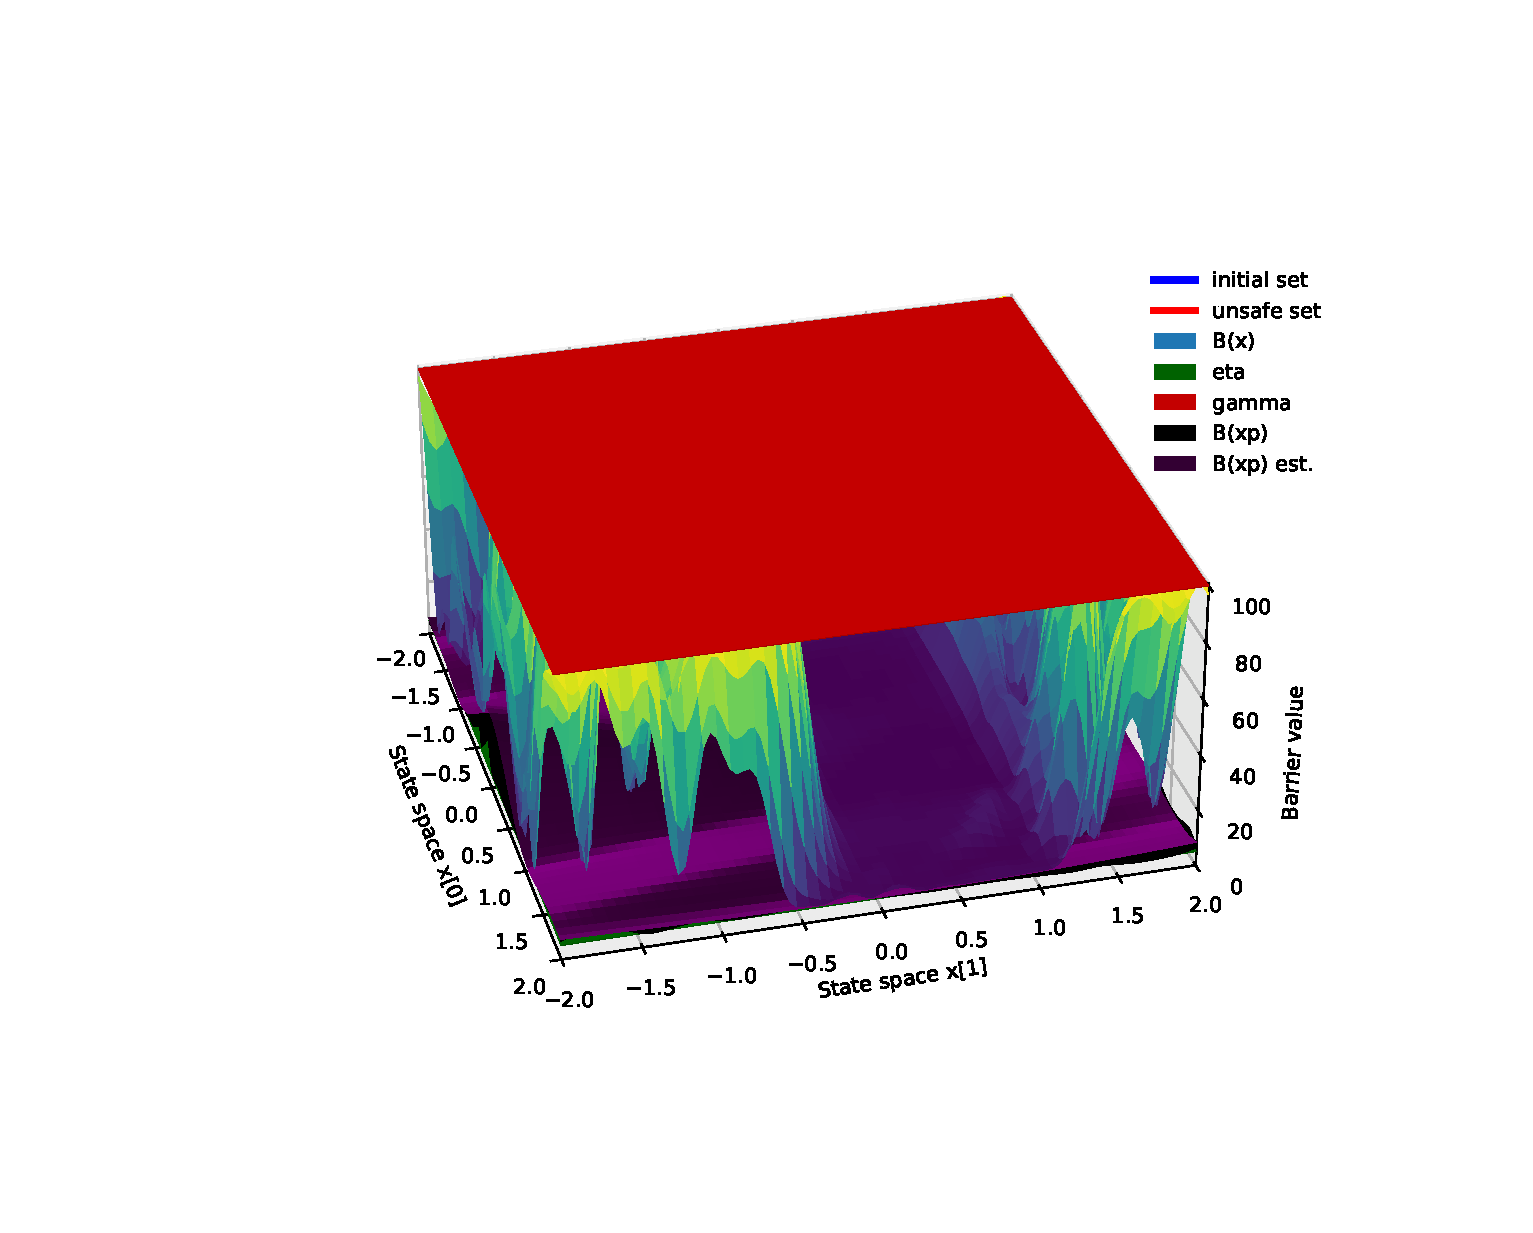
\includegraphics[trim={5cm 3cm 2cm 4cm},clip,width=\linewidth]{barrier2.pgf}
    \caption{\gls{cbc} synthesized for the \barrII benchmark.}
    \label{fig:CSBarr2}
\end{figure}

\begin{figure}[ht]
    \begin{adjustbox}{clip,trim=0cm 2cm 0cm 2cm,max width=\columnwidth}
        %% Creator: Matplotlib, PGF backend
%%
%% To include the figure in your LaTeX document, write
%%   \input{<filename>.pgf}
%%
%% Make sure the required packages are loaded in your preamble
%%   \usepackage{pgf}
%%
%% Also ensure that all the required font packages are loaded; for instance,
%% the lmodern package is sometimes necessary when using math font.
%%   \usepackage{lmodern}
%%
%% Figures using additional raster images can only be included by \input if
%% they are in the same directory as the main LaTeX file. For loading figures
%% from other directories you can use the `import` package
%%   \usepackage{import}
%%
%% and then include the figures with
%%   \import{<path to file>}{<filename>.pgf}
%%
%% Matplotlib used the following preamble
%%   \def\mathdefault#1{#1}
%%   \everymath=\expandafter{\the\everymath\displaystyle}
%%   \IfFileExists{scrextend.sty}{
%%     \usepackage[fontsize=10.000000pt]{scrextend}
%%   }{
%%     \renewcommand{\normalsize}{\fontsize{10.000000}{12.000000}\selectfont}
%%     \normalsize
%%   }
%%   
%%   \ifdefined\pdftexversion\else  % non-pdftex case.
%%     \usepackage{fontspec}
%%     \setmainfont{DejaVuSerif.ttf}[Path=\detokenize{/home/campus.ncl.ac.uk/c3054737/miniconda3/envs/dlinear/lib/python3.11/site-packages/matplotlib/mpl-data/fonts/ttf/}]
%%     \setsansfont{DejaVuSans.ttf}[Path=\detokenize{/home/campus.ncl.ac.uk/c3054737/miniconda3/envs/dlinear/lib/python3.11/site-packages/matplotlib/mpl-data/fonts/ttf/}]
%%     \setmonofont{DejaVuSansMono.ttf}[Path=\detokenize{/home/campus.ncl.ac.uk/c3054737/miniconda3/envs/dlinear/lib/python3.11/site-packages/matplotlib/mpl-data/fonts/ttf/}]
%%   \fi
%%   \makeatletter\@ifpackageloaded{underscore}{}{\usepackage[strings]{underscore}}\makeatother
%%
\begingroup%
\makeatletter%
\begin{pgfpicture}%
\pgfpathrectangle{\pgfpointorigin}{\pgfqpoint{6.400000in}{4.800000in}}%
\pgfusepath{use as bounding box, clip}%
\begin{pgfscope}%
\pgfsetbuttcap%
\pgfsetmiterjoin%
\definecolor{currentfill}{rgb}{1.000000,1.000000,1.000000}%
\pgfsetfillcolor{currentfill}%
\pgfsetlinewidth{0.000000pt}%
\definecolor{currentstroke}{rgb}{1.000000,1.000000,1.000000}%
\pgfsetstrokecolor{currentstroke}%
\pgfsetdash{}{0pt}%
\pgfpathmoveto{\pgfqpoint{0.000000in}{0.000000in}}%
\pgfpathlineto{\pgfqpoint{6.400000in}{0.000000in}}%
\pgfpathlineto{\pgfqpoint{6.400000in}{4.800000in}}%
\pgfpathlineto{\pgfqpoint{0.000000in}{4.800000in}}%
\pgfpathlineto{\pgfqpoint{0.000000in}{0.000000in}}%
\pgfpathclose%
\pgfusepath{fill}%
\end{pgfscope}%
\begin{pgfscope}%
\pgfsetbuttcap%
\pgfsetmiterjoin%
\definecolor{currentfill}{rgb}{1.000000,1.000000,1.000000}%
\pgfsetfillcolor{currentfill}%
\pgfsetlinewidth{0.000000pt}%
\definecolor{currentstroke}{rgb}{0.000000,0.000000,0.000000}%
\pgfsetstrokecolor{currentstroke}%
\pgfsetstrokeopacity{0.000000}%
\pgfsetdash{}{0pt}%
\pgfpathmoveto{\pgfqpoint{0.824000in}{0.528000in}}%
\pgfpathlineto{\pgfqpoint{4.520000in}{0.528000in}}%
\pgfpathlineto{\pgfqpoint{4.520000in}{4.224000in}}%
\pgfpathlineto{\pgfqpoint{0.824000in}{4.224000in}}%
\pgfpathlineto{\pgfqpoint{0.824000in}{0.528000in}}%
\pgfpathclose%
\pgfusepath{fill}%
\end{pgfscope}%
\begin{pgfscope}%
\pgfsetbuttcap%
\pgfsetmiterjoin%
\definecolor{currentfill}{rgb}{0.950000,0.950000,0.950000}%
\pgfsetfillcolor{currentfill}%
\pgfsetfillopacity{0.500000}%
\pgfsetlinewidth{1.003750pt}%
\definecolor{currentstroke}{rgb}{0.950000,0.950000,0.950000}%
\pgfsetstrokecolor{currentstroke}%
\pgfsetstrokeopacity{0.500000}%
\pgfsetdash{}{0pt}%
\pgfpathmoveto{\pgfqpoint{1.208997in}{1.279043in}}%
\pgfpathlineto{\pgfqpoint{1.895317in}{2.306186in}}%
\pgfpathlineto{\pgfqpoint{1.936396in}{3.833181in}}%
\pgfpathlineto{\pgfqpoint{1.225922in}{2.932113in}}%
\pgfusepath{stroke,fill}%
\end{pgfscope}%
\begin{pgfscope}%
\pgfsetbuttcap%
\pgfsetmiterjoin%
\definecolor{currentfill}{rgb}{0.900000,0.900000,0.900000}%
\pgfsetfillcolor{currentfill}%
\pgfsetfillopacity{0.500000}%
\pgfsetlinewidth{1.003750pt}%
\definecolor{currentstroke}{rgb}{0.900000,0.900000,0.900000}%
\pgfsetstrokecolor{currentstroke}%
\pgfsetstrokeopacity{0.500000}%
\pgfsetdash{}{0pt}%
\pgfpathmoveto{\pgfqpoint{1.895317in}{2.306186in}}%
\pgfpathlineto{\pgfqpoint{4.049663in}{1.976724in}}%
\pgfpathlineto{\pgfqpoint{4.174759in}{3.527263in}}%
\pgfpathlineto{\pgfqpoint{1.936396in}{3.833181in}}%
\pgfusepath{stroke,fill}%
\end{pgfscope}%
\begin{pgfscope}%
\pgfsetbuttcap%
\pgfsetmiterjoin%
\definecolor{currentfill}{rgb}{0.925000,0.925000,0.925000}%
\pgfsetfillcolor{currentfill}%
\pgfsetfillopacity{0.500000}%
\pgfsetlinewidth{1.003750pt}%
\definecolor{currentstroke}{rgb}{0.925000,0.925000,0.925000}%
\pgfsetstrokecolor{currentstroke}%
\pgfsetstrokeopacity{0.500000}%
\pgfsetdash{}{0pt}%
\pgfpathmoveto{\pgfqpoint{1.208997in}{1.279043in}}%
\pgfpathlineto{\pgfqpoint{3.580654in}{0.887656in}}%
\pgfpathlineto{\pgfqpoint{4.049663in}{1.976724in}}%
\pgfpathlineto{\pgfqpoint{1.895317in}{2.306186in}}%
\pgfusepath{stroke,fill}%
\end{pgfscope}%
\begin{pgfscope}%
\pgfsetbuttcap%
\pgfsetroundjoin%
\pgfsetlinewidth{0.803000pt}%
\definecolor{currentstroke}{rgb}{0.690196,0.690196,0.690196}%
\pgfsetstrokecolor{currentstroke}%
\pgfsetdash{}{0pt}%
\pgfpathmoveto{\pgfqpoint{1.208997in}{1.279043in}}%
\pgfpathlineto{\pgfqpoint{1.895317in}{2.306186in}}%
\pgfpathlineto{\pgfqpoint{1.936396in}{3.833181in}}%
\pgfusepath{stroke}%
\end{pgfscope}%
\begin{pgfscope}%
\pgfsetbuttcap%
\pgfsetroundjoin%
\pgfsetlinewidth{0.803000pt}%
\definecolor{currentstroke}{rgb}{0.690196,0.690196,0.690196}%
\pgfsetstrokecolor{currentstroke}%
\pgfsetdash{}{0pt}%
\pgfpathmoveto{\pgfqpoint{1.631448in}{1.209327in}}%
\pgfpathlineto{\pgfqpoint{2.279826in}{2.247384in}}%
\pgfpathlineto{\pgfqpoint{2.335618in}{3.778619in}}%
\pgfusepath{stroke}%
\end{pgfscope}%
\begin{pgfscope}%
\pgfsetbuttcap%
\pgfsetroundjoin%
\pgfsetlinewidth{0.803000pt}%
\definecolor{currentstroke}{rgb}{0.690196,0.690196,0.690196}%
\pgfsetstrokecolor{currentstroke}%
\pgfsetdash{}{0pt}%
\pgfpathmoveto{\pgfqpoint{2.057729in}{1.138979in}}%
\pgfpathlineto{\pgfqpoint{2.667485in}{2.188099in}}%
\pgfpathlineto{\pgfqpoint{2.738235in}{3.723593in}}%
\pgfusepath{stroke}%
\end{pgfscope}%
\begin{pgfscope}%
\pgfsetbuttcap%
\pgfsetroundjoin%
\pgfsetlinewidth{0.803000pt}%
\definecolor{currentstroke}{rgb}{0.690196,0.690196,0.690196}%
\pgfsetstrokecolor{currentstroke}%
\pgfsetdash{}{0pt}%
\pgfpathmoveto{\pgfqpoint{2.487895in}{1.067990in}}%
\pgfpathlineto{\pgfqpoint{3.058333in}{2.128327in}}%
\pgfpathlineto{\pgfqpoint{3.144290in}{3.668098in}}%
\pgfusepath{stroke}%
\end{pgfscope}%
\begin{pgfscope}%
\pgfsetbuttcap%
\pgfsetroundjoin%
\pgfsetlinewidth{0.803000pt}%
\definecolor{currentstroke}{rgb}{0.690196,0.690196,0.690196}%
\pgfsetstrokecolor{currentstroke}%
\pgfsetdash{}{0pt}%
\pgfpathmoveto{\pgfqpoint{2.921998in}{0.996352in}}%
\pgfpathlineto{\pgfqpoint{3.452409in}{2.068062in}}%
\pgfpathlineto{\pgfqpoint{3.553827in}{3.612126in}}%
\pgfusepath{stroke}%
\end{pgfscope}%
\begin{pgfscope}%
\pgfsetbuttcap%
\pgfsetroundjoin%
\pgfsetlinewidth{0.803000pt}%
\definecolor{currentstroke}{rgb}{0.690196,0.690196,0.690196}%
\pgfsetstrokecolor{currentstroke}%
\pgfsetdash{}{0pt}%
\pgfpathmoveto{\pgfqpoint{3.360092in}{0.924054in}}%
\pgfpathlineto{\pgfqpoint{3.849753in}{2.007296in}}%
\pgfpathlineto{\pgfqpoint{3.966890in}{3.555672in}}%
\pgfusepath{stroke}%
\end{pgfscope}%
\begin{pgfscope}%
\pgfsetbuttcap%
\pgfsetroundjoin%
\pgfsetlinewidth{0.803000pt}%
\definecolor{currentstroke}{rgb}{0.690196,0.690196,0.690196}%
\pgfsetstrokecolor{currentstroke}%
\pgfsetdash{}{0pt}%
\pgfpathmoveto{\pgfqpoint{1.225922in}{2.932113in}}%
\pgfpathlineto{\pgfqpoint{1.208997in}{1.279043in}}%
\pgfpathlineto{\pgfqpoint{3.580654in}{0.887656in}}%
\pgfusepath{stroke}%
\end{pgfscope}%
\begin{pgfscope}%
\pgfsetbuttcap%
\pgfsetroundjoin%
\pgfsetlinewidth{0.803000pt}%
\definecolor{currentstroke}{rgb}{0.690196,0.690196,0.690196}%
\pgfsetstrokecolor{currentstroke}%
\pgfsetdash{}{0pt}%
\pgfpathmoveto{\pgfqpoint{1.355059in}{3.095893in}}%
\pgfpathlineto{\pgfqpoint{1.333336in}{1.465127in}}%
\pgfpathlineto{\pgfqpoint{3.665792in}{1.085352in}}%
\pgfusepath{stroke}%
\end{pgfscope}%
\begin{pgfscope}%
\pgfsetbuttcap%
\pgfsetroundjoin%
\pgfsetlinewidth{0.803000pt}%
\definecolor{currentstroke}{rgb}{0.690196,0.690196,0.690196}%
\pgfsetstrokecolor{currentstroke}%
\pgfsetdash{}{0pt}%
\pgfpathmoveto{\pgfqpoint{1.479601in}{3.253845in}}%
\pgfpathlineto{\pgfqpoint{1.453421in}{1.644847in}}%
\pgfpathlineto{\pgfqpoint{3.747947in}{1.276121in}}%
\pgfusepath{stroke}%
\end{pgfscope}%
\begin{pgfscope}%
\pgfsetbuttcap%
\pgfsetroundjoin%
\pgfsetlinewidth{0.803000pt}%
\definecolor{currentstroke}{rgb}{0.690196,0.690196,0.690196}%
\pgfsetstrokecolor{currentstroke}%
\pgfsetdash{}{0pt}%
\pgfpathmoveto{\pgfqpoint{1.599789in}{3.406275in}}%
\pgfpathlineto{\pgfqpoint{1.569468in}{1.818522in}}%
\pgfpathlineto{\pgfqpoint{3.827273in}{1.460320in}}%
\pgfusepath{stroke}%
\end{pgfscope}%
\begin{pgfscope}%
\pgfsetbuttcap%
\pgfsetroundjoin%
\pgfsetlinewidth{0.803000pt}%
\definecolor{currentstroke}{rgb}{0.690196,0.690196,0.690196}%
\pgfsetstrokecolor{currentstroke}%
\pgfsetdash{}{0pt}%
\pgfpathmoveto{\pgfqpoint{1.715847in}{3.553467in}}%
\pgfpathlineto{\pgfqpoint{1.681677in}{1.986453in}}%
\pgfpathlineto{\pgfqpoint{3.903912in}{1.638282in}}%
\pgfusepath{stroke}%
\end{pgfscope}%
\begin{pgfscope}%
\pgfsetbuttcap%
\pgfsetroundjoin%
\pgfsetlinewidth{0.803000pt}%
\definecolor{currentstroke}{rgb}{0.690196,0.690196,0.690196}%
\pgfsetstrokecolor{currentstroke}%
\pgfsetdash{}{0pt}%
\pgfpathmoveto{\pgfqpoint{1.827984in}{3.695686in}}%
\pgfpathlineto{\pgfqpoint{1.790235in}{2.148920in}}%
\pgfpathlineto{\pgfqpoint{3.978001in}{1.810320in}}%
\pgfusepath{stroke}%
\end{pgfscope}%
\begin{pgfscope}%
\pgfsetbuttcap%
\pgfsetroundjoin%
\pgfsetlinewidth{0.803000pt}%
\definecolor{currentstroke}{rgb}{0.690196,0.690196,0.690196}%
\pgfsetstrokecolor{currentstroke}%
\pgfsetdash{}{0pt}%
\pgfpathmoveto{\pgfqpoint{1.936396in}{3.833181in}}%
\pgfpathlineto{\pgfqpoint{1.895317in}{2.306186in}}%
\pgfpathlineto{\pgfqpoint{4.049663in}{1.976724in}}%
\pgfusepath{stroke}%
\end{pgfscope}%
\begin{pgfscope}%
\pgfsetbuttcap%
\pgfsetroundjoin%
\pgfsetlinewidth{0.803000pt}%
\definecolor{currentstroke}{rgb}{0.690196,0.690196,0.690196}%
\pgfsetstrokecolor{currentstroke}%
\pgfsetdash{}{0pt}%
\pgfpathmoveto{\pgfqpoint{4.049663in}{1.976724in}}%
\pgfpathlineto{\pgfqpoint{1.895317in}{2.306186in}}%
\pgfpathlineto{\pgfqpoint{1.208997in}{1.279043in}}%
\pgfusepath{stroke}%
\end{pgfscope}%
\begin{pgfscope}%
\pgfsetbuttcap%
\pgfsetroundjoin%
\pgfsetlinewidth{0.803000pt}%
\definecolor{currentstroke}{rgb}{0.690196,0.690196,0.690196}%
\pgfsetstrokecolor{currentstroke}%
\pgfsetdash{}{0pt}%
\pgfpathmoveto{\pgfqpoint{4.069864in}{2.227105in}}%
\pgfpathlineto{\pgfqpoint{1.901955in}{2.552943in}}%
\pgfpathlineto{\pgfqpoint{1.211723in}{1.545276in}}%
\pgfusepath{stroke}%
\end{pgfscope}%
\begin{pgfscope}%
\pgfsetbuttcap%
\pgfsetroundjoin%
\pgfsetlinewidth{0.803000pt}%
\definecolor{currentstroke}{rgb}{0.690196,0.690196,0.690196}%
\pgfsetstrokecolor{currentstroke}%
\pgfsetdash{}{0pt}%
\pgfpathmoveto{\pgfqpoint{4.090317in}{2.480622in}}%
\pgfpathlineto{\pgfqpoint{1.908675in}{2.802720in}}%
\pgfpathlineto{\pgfqpoint{1.214486in}{1.815120in}}%
\pgfusepath{stroke}%
\end{pgfscope}%
\begin{pgfscope}%
\pgfsetbuttcap%
\pgfsetroundjoin%
\pgfsetlinewidth{0.803000pt}%
\definecolor{currentstroke}{rgb}{0.690196,0.690196,0.690196}%
\pgfsetstrokecolor{currentstroke}%
\pgfsetdash{}{0pt}%
\pgfpathmoveto{\pgfqpoint{4.111028in}{2.737334in}}%
\pgfpathlineto{\pgfqpoint{1.915477in}{3.055575in}}%
\pgfpathlineto{\pgfqpoint{1.217286in}{2.088649in}}%
\pgfusepath{stroke}%
\end{pgfscope}%
\begin{pgfscope}%
\pgfsetbuttcap%
\pgfsetroundjoin%
\pgfsetlinewidth{0.803000pt}%
\definecolor{currentstroke}{rgb}{0.690196,0.690196,0.690196}%
\pgfsetstrokecolor{currentstroke}%
\pgfsetdash{}{0pt}%
\pgfpathmoveto{\pgfqpoint{4.132003in}{2.997304in}}%
\pgfpathlineto{\pgfqpoint{1.922364in}{3.311564in}}%
\pgfpathlineto{\pgfqpoint{1.220125in}{2.365938in}}%
\pgfusepath{stroke}%
\end{pgfscope}%
\begin{pgfscope}%
\pgfsetbuttcap%
\pgfsetroundjoin%
\pgfsetlinewidth{0.803000pt}%
\definecolor{currentstroke}{rgb}{0.690196,0.690196,0.690196}%
\pgfsetstrokecolor{currentstroke}%
\pgfsetdash{}{0pt}%
\pgfpathmoveto{\pgfqpoint{4.153244in}{3.260592in}}%
\pgfpathlineto{\pgfqpoint{1.929336in}{3.570746in}}%
\pgfpathlineto{\pgfqpoint{1.223003in}{2.647066in}}%
\pgfusepath{stroke}%
\end{pgfscope}%
\begin{pgfscope}%
\pgfsetbuttcap%
\pgfsetroundjoin%
\pgfsetlinewidth{0.803000pt}%
\definecolor{currentstroke}{rgb}{0.690196,0.690196,0.690196}%
\pgfsetstrokecolor{currentstroke}%
\pgfsetdash{}{0pt}%
\pgfpathmoveto{\pgfqpoint{4.174759in}{3.527263in}}%
\pgfpathlineto{\pgfqpoint{1.936396in}{3.833181in}}%
\pgfpathlineto{\pgfqpoint{1.225922in}{2.932113in}}%
\pgfusepath{stroke}%
\end{pgfscope}%
\begin{pgfscope}%
\pgfsetrectcap%
\pgfsetroundjoin%
\pgfsetlinewidth{0.803000pt}%
\definecolor{currentstroke}{rgb}{0.000000,0.000000,0.000000}%
\pgfsetstrokecolor{currentstroke}%
\pgfsetdash{}{0pt}%
\pgfpathmoveto{\pgfqpoint{1.208997in}{1.279043in}}%
\pgfpathlineto{\pgfqpoint{3.580654in}{0.887656in}}%
\pgfusepath{stroke}%
\end{pgfscope}%
\begin{pgfscope}%
\pgfsetrectcap%
\pgfsetroundjoin%
\pgfsetlinewidth{0.803000pt}%
\definecolor{currentstroke}{rgb}{0.000000,0.000000,0.000000}%
\pgfsetstrokecolor{currentstroke}%
\pgfsetdash{}{0pt}%
\pgfpathmoveto{\pgfqpoint{1.215066in}{1.288125in}}%
\pgfpathlineto{\pgfqpoint{1.196829in}{1.260831in}}%
\pgfusepath{stroke}%
\end{pgfscope}%
\begin{pgfscope}%
\definecolor{textcolor}{rgb}{0.000000,0.000000,0.000000}%
\pgfsetstrokecolor{textcolor}%
\pgfsetfillcolor{textcolor}%
\pgftext[x=1.144298in,y=1.051863in,,top]{\color{textcolor}{\sffamily\fontsize{10.000000}{12.000000}\selectfont\catcode`\^=\active\def^{\ifmmode\sp\else\^{}\fi}\catcode`\%=\active\def%{\%}\ensuremath{-}3}}%
\end{pgfscope}%
\begin{pgfscope}%
\pgfsetrectcap%
\pgfsetroundjoin%
\pgfsetlinewidth{0.803000pt}%
\definecolor{currentstroke}{rgb}{0.000000,0.000000,0.000000}%
\pgfsetstrokecolor{currentstroke}%
\pgfsetdash{}{0pt}%
\pgfpathmoveto{\pgfqpoint{1.637183in}{1.218510in}}%
\pgfpathlineto{\pgfqpoint{1.619947in}{1.190914in}}%
\pgfusepath{stroke}%
\end{pgfscope}%
\begin{pgfscope}%
\definecolor{textcolor}{rgb}{0.000000,0.000000,0.000000}%
\pgfsetstrokecolor{textcolor}%
\pgfsetfillcolor{textcolor}%
\pgftext[x=1.568795in,y=0.980730in,,top]{\color{textcolor}{\sffamily\fontsize{10.000000}{12.000000}\selectfont\catcode`\^=\active\def^{\ifmmode\sp\else\^{}\fi}\catcode`\%=\active\def%{\%}\ensuremath{-}2}}%
\end{pgfscope}%
\begin{pgfscope}%
\pgfsetrectcap%
\pgfsetroundjoin%
\pgfsetlinewidth{0.803000pt}%
\definecolor{currentstroke}{rgb}{0.000000,0.000000,0.000000}%
\pgfsetstrokecolor{currentstroke}%
\pgfsetdash{}{0pt}%
\pgfpathmoveto{\pgfqpoint{2.063126in}{1.148264in}}%
\pgfpathlineto{\pgfqpoint{2.046909in}{1.120362in}}%
\pgfusepath{stroke}%
\end{pgfscope}%
\begin{pgfscope}%
\definecolor{textcolor}{rgb}{0.000000,0.000000,0.000000}%
\pgfsetstrokecolor{textcolor}%
\pgfsetfillcolor{textcolor}%
\pgftext[x=1.997164in,y=0.908948in,,top]{\color{textcolor}{\sffamily\fontsize{10.000000}{12.000000}\selectfont\catcode`\^=\active\def^{\ifmmode\sp\else\^{}\fi}\catcode`\%=\active\def%{\%}\ensuremath{-}1}}%
\end{pgfscope}%
\begin{pgfscope}%
\pgfsetrectcap%
\pgfsetroundjoin%
\pgfsetlinewidth{0.803000pt}%
\definecolor{currentstroke}{rgb}{0.000000,0.000000,0.000000}%
\pgfsetstrokecolor{currentstroke}%
\pgfsetdash{}{0pt}%
\pgfpathmoveto{\pgfqpoint{2.492946in}{1.077379in}}%
\pgfpathlineto{\pgfqpoint{2.477768in}{1.049165in}}%
\pgfusepath{stroke}%
\end{pgfscope}%
\begin{pgfscope}%
\definecolor{textcolor}{rgb}{0.000000,0.000000,0.000000}%
\pgfsetstrokecolor{textcolor}%
\pgfsetfillcolor{textcolor}%
\pgftext[x=2.429458in,y=0.836508in,,top]{\color{textcolor}{\sffamily\fontsize{10.000000}{12.000000}\selectfont\catcode`\^=\active\def^{\ifmmode\sp\else\^{}\fi}\catcode`\%=\active\def%{\%}0}}%
\end{pgfscope}%
\begin{pgfscope}%
\pgfsetrectcap%
\pgfsetroundjoin%
\pgfsetlinewidth{0.803000pt}%
\definecolor{currentstroke}{rgb}{0.000000,0.000000,0.000000}%
\pgfsetstrokecolor{currentstroke}%
\pgfsetdash{}{0pt}%
\pgfpathmoveto{\pgfqpoint{2.926696in}{1.005845in}}%
\pgfpathlineto{\pgfqpoint{2.912577in}{0.977316in}}%
\pgfusepath{stroke}%
\end{pgfscope}%
\begin{pgfscope}%
\definecolor{textcolor}{rgb}{0.000000,0.000000,0.000000}%
\pgfsetstrokecolor{textcolor}%
\pgfsetfillcolor{textcolor}%
\pgftext[x=2.865730in,y=0.763402in,,top]{\color{textcolor}{\sffamily\fontsize{10.000000}{12.000000}\selectfont\catcode`\^=\active\def^{\ifmmode\sp\else\^{}\fi}\catcode`\%=\active\def%{\%}1}}%
\end{pgfscope}%
\begin{pgfscope}%
\pgfsetrectcap%
\pgfsetroundjoin%
\pgfsetlinewidth{0.803000pt}%
\definecolor{currentstroke}{rgb}{0.000000,0.000000,0.000000}%
\pgfsetstrokecolor{currentstroke}%
\pgfsetdash{}{0pt}%
\pgfpathmoveto{\pgfqpoint{3.364432in}{0.933654in}}%
\pgfpathlineto{\pgfqpoint{3.351391in}{0.904805in}}%
\pgfusepath{stroke}%
\end{pgfscope}%
\begin{pgfscope}%
\definecolor{textcolor}{rgb}{0.000000,0.000000,0.000000}%
\pgfsetstrokecolor{textcolor}%
\pgfsetfillcolor{textcolor}%
\pgftext[x=3.306037in,y=0.689620in,,top]{\color{textcolor}{\sffamily\fontsize{10.000000}{12.000000}\selectfont\catcode`\^=\active\def^{\ifmmode\sp\else\^{}\fi}\catcode`\%=\active\def%{\%}2}}%
\end{pgfscope}%
\begin{pgfscope}%
\definecolor{textcolor}{rgb}{0.000000,0.000000,0.000000}%
\pgfsetstrokecolor{textcolor}%
\pgfsetfillcolor{textcolor}%
\pgftext[x=2.250938in,y=0.580052in,,,rotate=350.629118]{\color{textcolor}{\sffamily\fontsize{10.000000}{12.000000}\selectfont\catcode`\^=\active\def^{\ifmmode\sp\else\^{}\fi}\catcode`\%=\active\def%{\%}State space x[0]}}%
\end{pgfscope}%
\begin{pgfscope}%
\pgfsetrectcap%
\pgfsetroundjoin%
\pgfsetlinewidth{0.803000pt}%
\definecolor{currentstroke}{rgb}{0.000000,0.000000,0.000000}%
\pgfsetstrokecolor{currentstroke}%
\pgfsetdash{}{0pt}%
\pgfpathmoveto{\pgfqpoint{4.049663in}{1.976724in}}%
\pgfpathlineto{\pgfqpoint{3.580654in}{0.887656in}}%
\pgfusepath{stroke}%
\end{pgfscope}%
\begin{pgfscope}%
\pgfsetrectcap%
\pgfsetroundjoin%
\pgfsetlinewidth{0.803000pt}%
\definecolor{currentstroke}{rgb}{0.000000,0.000000,0.000000}%
\pgfsetstrokecolor{currentstroke}%
\pgfsetdash{}{0pt}%
\pgfpathmoveto{\pgfqpoint{3.561204in}{0.890866in}}%
\pgfpathlineto{\pgfqpoint{3.619578in}{0.881232in}}%
\pgfusepath{stroke}%
\end{pgfscope}%
\begin{pgfscope}%
\definecolor{textcolor}{rgb}{0.000000,0.000000,0.000000}%
\pgfsetstrokecolor{textcolor}%
\pgfsetfillcolor{textcolor}%
\pgftext[x=3.772690in,y=0.720923in,,top]{\color{textcolor}{\sffamily\fontsize{10.000000}{12.000000}\selectfont\catcode`\^=\active\def^{\ifmmode\sp\else\^{}\fi}\catcode`\%=\active\def%{\%}\ensuremath{-}2.0}}%
\end{pgfscope}%
\begin{pgfscope}%
\pgfsetrectcap%
\pgfsetroundjoin%
\pgfsetlinewidth{0.803000pt}%
\definecolor{currentstroke}{rgb}{0.000000,0.000000,0.000000}%
\pgfsetstrokecolor{currentstroke}%
\pgfsetdash{}{0pt}%
\pgfpathmoveto{\pgfqpoint{3.646672in}{1.088465in}}%
\pgfpathlineto{\pgfqpoint{3.704056in}{1.079122in}}%
\pgfusepath{stroke}%
\end{pgfscope}%
\begin{pgfscope}%
\definecolor{textcolor}{rgb}{0.000000,0.000000,0.000000}%
\pgfsetstrokecolor{textcolor}%
\pgfsetfillcolor{textcolor}%
\pgftext[x=3.854299in,y=0.921335in,,top]{\color{textcolor}{\sffamily\fontsize{10.000000}{12.000000}\selectfont\catcode`\^=\active\def^{\ifmmode\sp\else\^{}\fi}\catcode`\%=\active\def%{\%}\ensuremath{-}1.5}}%
\end{pgfscope}%
\begin{pgfscope}%
\pgfsetrectcap%
\pgfsetroundjoin%
\pgfsetlinewidth{0.803000pt}%
\definecolor{currentstroke}{rgb}{0.000000,0.000000,0.000000}%
\pgfsetstrokecolor{currentstroke}%
\pgfsetdash{}{0pt}%
\pgfpathmoveto{\pgfqpoint{3.729146in}{1.279142in}}%
\pgfpathlineto{\pgfqpoint{3.785572in}{1.270075in}}%
\pgfusepath{stroke}%
\end{pgfscope}%
\begin{pgfscope}%
\definecolor{textcolor}{rgb}{0.000000,0.000000,0.000000}%
\pgfsetstrokecolor{textcolor}%
\pgfsetfillcolor{textcolor}%
\pgftext[x=3.933051in,y=1.114733in,,top]{\color{textcolor}{\sffamily\fontsize{10.000000}{12.000000}\selectfont\catcode`\^=\active\def^{\ifmmode\sp\else\^{}\fi}\catcode`\%=\active\def%{\%}\ensuremath{-}1.0}}%
\end{pgfscope}%
\begin{pgfscope}%
\pgfsetrectcap%
\pgfsetroundjoin%
\pgfsetlinewidth{0.803000pt}%
\definecolor{currentstroke}{rgb}{0.000000,0.000000,0.000000}%
\pgfsetstrokecolor{currentstroke}%
\pgfsetdash{}{0pt}%
\pgfpathmoveto{\pgfqpoint{3.808780in}{1.463254in}}%
\pgfpathlineto{\pgfqpoint{3.864280in}{1.454449in}}%
\pgfusepath{stroke}%
\end{pgfscope}%
\begin{pgfscope}%
\definecolor{textcolor}{rgb}{0.000000,0.000000,0.000000}%
\pgfsetstrokecolor{textcolor}%
\pgfsetfillcolor{textcolor}%
\pgftext[x=4.009094in,y=1.301478in,,top]{\color{textcolor}{\sffamily\fontsize{10.000000}{12.000000}\selectfont\catcode`\^=\active\def^{\ifmmode\sp\else\^{}\fi}\catcode`\%=\active\def%{\%}\ensuremath{-}0.5}}%
\end{pgfscope}%
\begin{pgfscope}%
\pgfsetrectcap%
\pgfsetroundjoin%
\pgfsetlinewidth{0.803000pt}%
\definecolor{currentstroke}{rgb}{0.000000,0.000000,0.000000}%
\pgfsetstrokecolor{currentstroke}%
\pgfsetdash{}{0pt}%
\pgfpathmoveto{\pgfqpoint{3.885718in}{1.641133in}}%
\pgfpathlineto{\pgfqpoint{3.940322in}{1.632578in}}%
\pgfusepath{stroke}%
\end{pgfscope}%
\begin{pgfscope}%
\definecolor{textcolor}{rgb}{0.000000,0.000000,0.000000}%
\pgfsetstrokecolor{textcolor}%
\pgfsetfillcolor{textcolor}%
\pgftext[x=4.082567in,y=1.481909in,,top]{\color{textcolor}{\sffamily\fontsize{10.000000}{12.000000}\selectfont\catcode`\^=\active\def^{\ifmmode\sp\else\^{}\fi}\catcode`\%=\active\def%{\%}0.0}}%
\end{pgfscope}%
\begin{pgfscope}%
\pgfsetrectcap%
\pgfsetroundjoin%
\pgfsetlinewidth{0.803000pt}%
\definecolor{currentstroke}{rgb}{0.000000,0.000000,0.000000}%
\pgfsetstrokecolor{currentstroke}%
\pgfsetdash{}{0pt}%
\pgfpathmoveto{\pgfqpoint{3.960095in}{1.813091in}}%
\pgfpathlineto{\pgfqpoint{4.013832in}{1.804775in}}%
\pgfusepath{stroke}%
\end{pgfscope}%
\begin{pgfscope}%
\definecolor{textcolor}{rgb}{0.000000,0.000000,0.000000}%
\pgfsetstrokecolor{textcolor}%
\pgfsetfillcolor{textcolor}%
\pgftext[x=4.153596in,y=1.656340in,,top]{\color{textcolor}{\sffamily\fontsize{10.000000}{12.000000}\selectfont\catcode`\^=\active\def^{\ifmmode\sp\else\^{}\fi}\catcode`\%=\active\def%{\%}0.5}}%
\end{pgfscope}%
\begin{pgfscope}%
\pgfsetrectcap%
\pgfsetroundjoin%
\pgfsetlinewidth{0.803000pt}%
\definecolor{currentstroke}{rgb}{0.000000,0.000000,0.000000}%
\pgfsetstrokecolor{currentstroke}%
\pgfsetdash{}{0pt}%
\pgfpathmoveto{\pgfqpoint{4.032038in}{1.979420in}}%
\pgfpathlineto{\pgfqpoint{4.084933in}{1.971330in}}%
\pgfusepath{stroke}%
\end{pgfscope}%
\begin{pgfscope}%
\definecolor{textcolor}{rgb}{0.000000,0.000000,0.000000}%
\pgfsetstrokecolor{textcolor}%
\pgfsetfillcolor{textcolor}%
\pgftext[x=4.222301in,y=1.825065in,,top]{\color{textcolor}{\sffamily\fontsize{10.000000}{12.000000}\selectfont\catcode`\^=\active\def^{\ifmmode\sp\else\^{}\fi}\catcode`\%=\active\def%{\%}1.0}}%
\end{pgfscope}%
\begin{pgfscope}%
\definecolor{textcolor}{rgb}{0.000000,0.000000,0.000000}%
\pgfsetstrokecolor{textcolor}%
\pgfsetfillcolor{textcolor}%
\pgftext[x=4.221962in,y=1.115515in,,,rotate=66.700783]{\color{textcolor}{\sffamily\fontsize{10.000000}{12.000000}\selectfont\catcode`\^=\active\def^{\ifmmode\sp\else\^{}\fi}\catcode`\%=\active\def%{\%}State space x[1]}}%
\end{pgfscope}%
\begin{pgfscope}%
\pgfsetrectcap%
\pgfsetroundjoin%
\pgfsetlinewidth{0.803000pt}%
\definecolor{currentstroke}{rgb}{0.000000,0.000000,0.000000}%
\pgfsetstrokecolor{currentstroke}%
\pgfsetdash{}{0pt}%
\pgfpathmoveto{\pgfqpoint{4.049663in}{1.976724in}}%
\pgfpathlineto{\pgfqpoint{4.174759in}{3.527263in}}%
\pgfusepath{stroke}%
\end{pgfscope}%
\begin{pgfscope}%
\pgfsetrectcap%
\pgfsetroundjoin%
\pgfsetlinewidth{0.803000pt}%
\definecolor{currentstroke}{rgb}{0.000000,0.000000,0.000000}%
\pgfsetstrokecolor{currentstroke}%
\pgfsetdash{}{0pt}%
\pgfpathmoveto{\pgfqpoint{4.032038in}{1.979420in}}%
\pgfpathlineto{\pgfqpoint{4.084933in}{1.971330in}}%
\pgfusepath{stroke}%
\end{pgfscope}%
\begin{pgfscope}%
\definecolor{textcolor}{rgb}{0.000000,0.000000,0.000000}%
\pgfsetstrokecolor{textcolor}%
\pgfsetfillcolor{textcolor}%
\pgftext[x=4.266237in,y=2.029916in,,top]{\color{textcolor}{\sffamily\fontsize{10.000000}{12.000000}\selectfont\catcode`\^=\active\def^{\ifmmode\sp\else\^{}\fi}\catcode`\%=\active\def%{\%}0.0}}%
\end{pgfscope}%
\begin{pgfscope}%
\pgfsetrectcap%
\pgfsetroundjoin%
\pgfsetlinewidth{0.803000pt}%
\definecolor{currentstroke}{rgb}{0.000000,0.000000,0.000000}%
\pgfsetstrokecolor{currentstroke}%
\pgfsetdash{}{0pt}%
\pgfpathmoveto{\pgfqpoint{4.052125in}{2.229771in}}%
\pgfpathlineto{\pgfqpoint{4.105361in}{2.221769in}}%
\pgfusepath{stroke}%
\end{pgfscope}%
\begin{pgfscope}%
\definecolor{textcolor}{rgb}{0.000000,0.000000,0.000000}%
\pgfsetstrokecolor{textcolor}%
\pgfsetfillcolor{textcolor}%
\pgftext[x=4.287651in,y=2.279059in,,top]{\color{textcolor}{\sffamily\fontsize{10.000000}{12.000000}\selectfont\catcode`\^=\active\def^{\ifmmode\sp\else\^{}\fi}\catcode`\%=\active\def%{\%}0.5}}%
\end{pgfscope}%
\begin{pgfscope}%
\pgfsetrectcap%
\pgfsetroundjoin%
\pgfsetlinewidth{0.803000pt}%
\definecolor{currentstroke}{rgb}{0.000000,0.000000,0.000000}%
\pgfsetstrokecolor{currentstroke}%
\pgfsetdash{}{0pt}%
\pgfpathmoveto{\pgfqpoint{4.072463in}{2.483258in}}%
\pgfpathlineto{\pgfqpoint{4.126044in}{2.475347in}}%
\pgfusepath{stroke}%
\end{pgfscope}%
\begin{pgfscope}%
\definecolor{textcolor}{rgb}{0.000000,0.000000,0.000000}%
\pgfsetstrokecolor{textcolor}%
\pgfsetfillcolor{textcolor}%
\pgftext[x=4.309331in,y=2.531304in,,top]{\color{textcolor}{\sffamily\fontsize{10.000000}{12.000000}\selectfont\catcode`\^=\active\def^{\ifmmode\sp\else\^{}\fi}\catcode`\%=\active\def%{\%}1.0}}%
\end{pgfscope}%
\begin{pgfscope}%
\pgfsetrectcap%
\pgfsetroundjoin%
\pgfsetlinewidth{0.803000pt}%
\definecolor{currentstroke}{rgb}{0.000000,0.000000,0.000000}%
\pgfsetstrokecolor{currentstroke}%
\pgfsetdash{}{0pt}%
\pgfpathmoveto{\pgfqpoint{4.093058in}{2.739939in}}%
\pgfpathlineto{\pgfqpoint{4.146989in}{2.732122in}}%
\pgfusepath{stroke}%
\end{pgfscope}%
\begin{pgfscope}%
\definecolor{textcolor}{rgb}{0.000000,0.000000,0.000000}%
\pgfsetstrokecolor{textcolor}%
\pgfsetfillcolor{textcolor}%
\pgftext[x=4.331283in,y=2.786708in,,top]{\color{textcolor}{\sffamily\fontsize{10.000000}{12.000000}\selectfont\catcode`\^=\active\def^{\ifmmode\sp\else\^{}\fi}\catcode`\%=\active\def%{\%}1.5}}%
\end{pgfscope}%
\begin{pgfscope}%
\pgfsetrectcap%
\pgfsetroundjoin%
\pgfsetlinewidth{0.803000pt}%
\definecolor{currentstroke}{rgb}{0.000000,0.000000,0.000000}%
\pgfsetstrokecolor{currentstroke}%
\pgfsetdash{}{0pt}%
\pgfpathmoveto{\pgfqpoint{4.113915in}{2.999876in}}%
\pgfpathlineto{\pgfqpoint{4.168199in}{2.992156in}}%
\pgfusepath{stroke}%
\end{pgfscope}%
\begin{pgfscope}%
\definecolor{textcolor}{rgb}{0.000000,0.000000,0.000000}%
\pgfsetstrokecolor{textcolor}%
\pgfsetfillcolor{textcolor}%
\pgftext[x=4.353512in,y=3.045332in,,top]{\color{textcolor}{\sffamily\fontsize{10.000000}{12.000000}\selectfont\catcode`\^=\active\def^{\ifmmode\sp\else\^{}\fi}\catcode`\%=\active\def%{\%}2.0}}%
\end{pgfscope}%
\begin{pgfscope}%
\pgfsetrectcap%
\pgfsetroundjoin%
\pgfsetlinewidth{0.803000pt}%
\definecolor{currentstroke}{rgb}{0.000000,0.000000,0.000000}%
\pgfsetstrokecolor{currentstroke}%
\pgfsetdash{}{0pt}%
\pgfpathmoveto{\pgfqpoint{4.135037in}{3.263131in}}%
\pgfpathlineto{\pgfqpoint{4.189680in}{3.255510in}}%
\pgfusepath{stroke}%
\end{pgfscope}%
\begin{pgfscope}%
\definecolor{textcolor}{rgb}{0.000000,0.000000,0.000000}%
\pgfsetstrokecolor{textcolor}%
\pgfsetfillcolor{textcolor}%
\pgftext[x=4.376022in,y=3.307236in,,top]{\color{textcolor}{\sffamily\fontsize{10.000000}{12.000000}\selectfont\catcode`\^=\active\def^{\ifmmode\sp\else\^{}\fi}\catcode`\%=\active\def%{\%}2.5}}%
\end{pgfscope}%
\begin{pgfscope}%
\pgfsetrectcap%
\pgfsetroundjoin%
\pgfsetlinewidth{0.803000pt}%
\definecolor{currentstroke}{rgb}{0.000000,0.000000,0.000000}%
\pgfsetstrokecolor{currentstroke}%
\pgfsetdash{}{0pt}%
\pgfpathmoveto{\pgfqpoint{4.156431in}{3.529768in}}%
\pgfpathlineto{\pgfqpoint{4.211437in}{3.522250in}}%
\pgfusepath{stroke}%
\end{pgfscope}%
\begin{pgfscope}%
\definecolor{textcolor}{rgb}{0.000000,0.000000,0.000000}%
\pgfsetstrokecolor{textcolor}%
\pgfsetfillcolor{textcolor}%
\pgftext[x=4.398820in,y=3.572484in,,top]{\color{textcolor}{\sffamily\fontsize{10.000000}{12.000000}\selectfont\catcode`\^=\active\def^{\ifmmode\sp\else\^{}\fi}\catcode`\%=\active\def%{\%}3.0}}%
\end{pgfscope}%
\begin{pgfscope}%
\definecolor{textcolor}{rgb}{0.000000,0.000000,0.000000}%
\pgfsetstrokecolor{textcolor}%
\pgfsetfillcolor{textcolor}%
\pgftext[x=4.586309in,y=2.843877in,,,rotate=85.387417]{\color{textcolor}{\sffamily\fontsize{10.000000}{12.000000}\selectfont\catcode`\^=\active\def^{\ifmmode\sp\else\^{}\fi}\catcode`\%=\active\def%{\%}Barrier value}}%
\end{pgfscope}%
\begin{pgfscope}%
\pgfpathrectangle{\pgfqpoint{0.824000in}{0.528000in}}{\pgfqpoint{3.696000in}{3.696000in}}%
\pgfusepath{clip}%
\pgfsetrectcap%
\pgfsetroundjoin%
\pgfsetlinewidth{1.505625pt}%
\definecolor{currentstroke}{rgb}{0.000000,0.000000,1.000000}%
\pgfsetstrokecolor{currentstroke}%
\pgfsetdash{}{0pt}%
\pgfpathmoveto{\pgfqpoint{3.200814in}{1.559708in}}%
\pgfpathlineto{\pgfqpoint{3.617543in}{1.493594in}}%
\pgfpathlineto{\pgfqpoint{3.774921in}{1.841751in}}%
\pgfpathlineto{\pgfqpoint{3.371318in}{1.904216in}}%
\pgfpathlineto{\pgfqpoint{3.200814in}{1.559708in}}%
\pgfusepath{stroke}%
\end{pgfscope}%
\begin{pgfscope}%
\pgfpathrectangle{\pgfqpoint{0.824000in}{0.528000in}}{\pgfqpoint{3.696000in}{3.696000in}}%
\pgfusepath{clip}%
\pgfsetrectcap%
\pgfsetroundjoin%
\pgfsetlinewidth{1.505625pt}%
\definecolor{currentstroke}{rgb}{0.000000,0.000000,1.000000}%
\pgfsetstrokecolor{currentstroke}%
\pgfsetdash{}{0pt}%
\pgfpathmoveto{\pgfqpoint{2.137066in}{1.878309in}}%
\pgfpathlineto{\pgfqpoint{2.377655in}{1.840521in}}%
\pgfpathlineto{\pgfqpoint{2.417361in}{1.907833in}}%
\pgfpathlineto{\pgfqpoint{2.178266in}{1.945202in}}%
\pgfpathlineto{\pgfqpoint{2.137066in}{1.878309in}}%
\pgfusepath{stroke}%
\end{pgfscope}%
\begin{pgfscope}%
\pgfpathrectangle{\pgfqpoint{0.824000in}{0.528000in}}{\pgfqpoint{3.696000in}{3.696000in}}%
\pgfusepath{clip}%
\pgfsetrectcap%
\pgfsetroundjoin%
\pgfsetlinewidth{1.505625pt}%
\definecolor{currentstroke}{rgb}{0.000000,0.000000,1.000000}%
\pgfsetstrokecolor{currentstroke}%
\pgfsetdash{}{0pt}%
\pgfpathmoveto{\pgfqpoint{2.215277in}{1.716064in}}%
\pgfpathlineto{\pgfqpoint{2.296628in}{1.703158in}}%
\pgfpathlineto{\pgfqpoint{2.417361in}{1.907833in}}%
\pgfpathlineto{\pgfqpoint{2.337529in}{1.920310in}}%
\pgfpathlineto{\pgfqpoint{2.215277in}{1.716064in}}%
\pgfusepath{stroke}%
\end{pgfscope}%
\begin{pgfscope}%
\pgfpathrectangle{\pgfqpoint{0.824000in}{0.528000in}}{\pgfqpoint{3.696000in}{3.696000in}}%
\pgfusepath{clip}%
\pgfsetrectcap%
\pgfsetroundjoin%
\pgfsetlinewidth{1.505625pt}%
\definecolor{currentstroke}{rgb}{1.000000,0.000000,0.000000}%
\pgfsetstrokecolor{currentstroke}%
\pgfsetdash{}{0pt}%
\pgfpathmoveto{\pgfqpoint{1.743042in}{2.013222in}}%
\pgfpathlineto{\pgfqpoint{1.782442in}{2.007065in}}%
\pgfpathlineto{\pgfqpoint{1.868047in}{2.136877in}}%
\pgfpathlineto{\pgfqpoint{1.829125in}{2.142901in}}%
\pgfpathlineto{\pgfqpoint{1.743042in}{2.013222in}}%
\pgfusepath{stroke}%
\end{pgfscope}%
\begin{pgfscope}%
\pgfpathrectangle{\pgfqpoint{0.824000in}{0.528000in}}{\pgfqpoint{3.696000in}{3.696000in}}%
\pgfusepath{clip}%
\pgfsetrectcap%
\pgfsetroundjoin%
\pgfsetlinewidth{1.505625pt}%
\definecolor{currentstroke}{rgb}{1.000000,0.000000,0.000000}%
\pgfsetstrokecolor{currentstroke}%
\pgfsetdash{}{0pt}%
\pgfpathmoveto{\pgfqpoint{1.743042in}{2.013222in}}%
\pgfpathlineto{\pgfqpoint{1.821875in}{2.000902in}}%
\pgfpathlineto{\pgfqpoint{1.864718in}{2.066301in}}%
\pgfpathlineto{\pgfqpoint{1.786365in}{2.078487in}}%
\pgfpathlineto{\pgfqpoint{1.743042in}{2.013222in}}%
\pgfusepath{stroke}%
\end{pgfscope}%
\begin{pgfscope}%
\pgfpathrectangle{\pgfqpoint{0.824000in}{0.528000in}}{\pgfqpoint{3.696000in}{3.696000in}}%
\pgfusepath{clip}%
\pgfsetbuttcap%
\pgfsetroundjoin%
\definecolor{currentfill}{rgb}{0.000000,0.000000,0.000000}%
\pgfsetfillcolor{currentfill}%
\pgfsetfillopacity{0.300000}%
\pgfsetlinewidth{0.000000pt}%
\definecolor{currentstroke}{rgb}{0.000000,0.000000,0.000000}%
\pgfsetstrokecolor{currentstroke}%
\pgfsetdash{}{0pt}%
\pgfpathmoveto{\pgfqpoint{1.873686in}{2.431787in}}%
\pgfpathlineto{\pgfqpoint{1.971697in}{2.751286in}}%
\pgfpathlineto{\pgfqpoint{1.994344in}{2.677484in}}%
\pgfpathlineto{\pgfqpoint{1.899338in}{2.455664in}}%
\pgfpathlineto{\pgfqpoint{1.873686in}{2.431787in}}%
\pgfpathclose%
\pgfusepath{fill}%
\end{pgfscope}%
\begin{pgfscope}%
\pgfpathrectangle{\pgfqpoint{0.824000in}{0.528000in}}{\pgfqpoint{3.696000in}{3.696000in}}%
\pgfusepath{clip}%
\pgfsetbuttcap%
\pgfsetroundjoin%
\definecolor{currentfill}{rgb}{0.000000,0.000000,0.000000}%
\pgfsetfillcolor{currentfill}%
\pgfsetfillopacity{0.300000}%
\pgfsetlinewidth{0.000000pt}%
\definecolor{currentstroke}{rgb}{0.000000,0.000000,0.000000}%
\pgfsetstrokecolor{currentstroke}%
\pgfsetdash{}{0pt}%
\pgfpathmoveto{\pgfqpoint{2.316826in}{2.332541in}}%
\pgfpathlineto{\pgfqpoint{2.406907in}{2.338803in}}%
\pgfpathlineto{\pgfqpoint{2.431750in}{2.398102in}}%
\pgfpathlineto{\pgfqpoint{2.340746in}{2.359914in}}%
\pgfpathlineto{\pgfqpoint{2.316826in}{2.332541in}}%
\pgfpathclose%
\pgfusepath{fill}%
\end{pgfscope}%
\begin{pgfscope}%
\pgfpathrectangle{\pgfqpoint{0.824000in}{0.528000in}}{\pgfqpoint{3.696000in}{3.696000in}}%
\pgfusepath{clip}%
\pgfsetbuttcap%
\pgfsetroundjoin%
\definecolor{currentfill}{rgb}{0.000000,0.000000,0.000000}%
\pgfsetfillcolor{currentfill}%
\pgfsetfillopacity{0.300000}%
\pgfsetlinewidth{0.000000pt}%
\definecolor{currentstroke}{rgb}{0.000000,0.000000,0.000000}%
\pgfsetstrokecolor{currentstroke}%
\pgfsetdash{}{0pt}%
\pgfpathmoveto{\pgfqpoint{2.051000in}{2.407670in}}%
\pgfpathlineto{\pgfqpoint{2.147030in}{2.612044in}}%
\pgfpathlineto{\pgfqpoint{2.170561in}{2.601606in}}%
\pgfpathlineto{\pgfqpoint{2.076278in}{2.442968in}}%
\pgfpathlineto{\pgfqpoint{2.051000in}{2.407670in}}%
\pgfpathclose%
\pgfusepath{fill}%
\end{pgfscope}%
\begin{pgfscope}%
\pgfpathrectangle{\pgfqpoint{0.824000in}{0.528000in}}{\pgfqpoint{3.696000in}{3.696000in}}%
\pgfusepath{clip}%
\pgfsetbuttcap%
\pgfsetroundjoin%
\definecolor{currentfill}{rgb}{0.000000,0.000000,0.000000}%
\pgfsetfillcolor{currentfill}%
\pgfsetfillopacity{0.300000}%
\pgfsetlinewidth{0.000000pt}%
\definecolor{currentstroke}{rgb}{0.000000,0.000000,0.000000}%
\pgfsetstrokecolor{currentstroke}%
\pgfsetdash{}{0pt}%
\pgfpathmoveto{\pgfqpoint{1.971697in}{2.751286in}}%
\pgfpathlineto{\pgfqpoint{2.051000in}{2.407670in}}%
\pgfpathlineto{\pgfqpoint{2.076278in}{2.442968in}}%
\pgfpathlineto{\pgfqpoint{1.994344in}{2.677484in}}%
\pgfpathlineto{\pgfqpoint{1.971697in}{2.751286in}}%
\pgfpathclose%
\pgfusepath{fill}%
\end{pgfscope}%
\begin{pgfscope}%
\pgfpathrectangle{\pgfqpoint{0.824000in}{0.528000in}}{\pgfqpoint{3.696000in}{3.696000in}}%
\pgfusepath{clip}%
\pgfsetbuttcap%
\pgfsetroundjoin%
\definecolor{currentfill}{rgb}{0.000000,0.000000,0.000000}%
\pgfsetfillcolor{currentfill}%
\pgfsetfillopacity{0.300000}%
\pgfsetlinewidth{0.000000pt}%
\definecolor{currentstroke}{rgb}{0.000000,0.000000,0.000000}%
\pgfsetstrokecolor{currentstroke}%
\pgfsetdash{}{0pt}%
\pgfpathmoveto{\pgfqpoint{2.406907in}{2.338803in}}%
\pgfpathlineto{\pgfqpoint{2.493637in}{2.258542in}}%
\pgfpathlineto{\pgfqpoint{2.518035in}{2.315227in}}%
\pgfpathlineto{\pgfqpoint{2.431750in}{2.398102in}}%
\pgfpathlineto{\pgfqpoint{2.406907in}{2.338803in}}%
\pgfpathclose%
\pgfusepath{fill}%
\end{pgfscope}%
\begin{pgfscope}%
\pgfpathrectangle{\pgfqpoint{0.824000in}{0.528000in}}{\pgfqpoint{3.696000in}{3.696000in}}%
\pgfusepath{clip}%
\pgfsetbuttcap%
\pgfsetroundjoin%
\definecolor{currentfill}{rgb}{0.000000,0.000000,0.000000}%
\pgfsetfillcolor{currentfill}%
\pgfsetfillopacity{0.300000}%
\pgfsetlinewidth{0.000000pt}%
\definecolor{currentstroke}{rgb}{0.000000,0.000000,0.000000}%
\pgfsetstrokecolor{currentstroke}%
\pgfsetdash{}{0pt}%
\pgfpathmoveto{\pgfqpoint{2.493637in}{2.258542in}}%
\pgfpathlineto{\pgfqpoint{2.584004in}{2.263938in}}%
\pgfpathlineto{\pgfqpoint{2.606348in}{2.281080in}}%
\pgfpathlineto{\pgfqpoint{2.518035in}{2.315227in}}%
\pgfpathlineto{\pgfqpoint{2.493637in}{2.258542in}}%
\pgfpathclose%
\pgfusepath{fill}%
\end{pgfscope}%
\begin{pgfscope}%
\pgfpathrectangle{\pgfqpoint{0.824000in}{0.528000in}}{\pgfqpoint{3.696000in}{3.696000in}}%
\pgfusepath{clip}%
\pgfsetbuttcap%
\pgfsetroundjoin%
\definecolor{currentfill}{rgb}{0.000000,0.000000,0.000000}%
\pgfsetfillcolor{currentfill}%
\pgfsetfillopacity{0.300000}%
\pgfsetlinewidth{0.000000pt}%
\definecolor{currentstroke}{rgb}{0.000000,0.000000,0.000000}%
\pgfsetstrokecolor{currentstroke}%
\pgfsetdash{}{0pt}%
\pgfpathmoveto{\pgfqpoint{2.584004in}{2.263938in}}%
\pgfpathlineto{\pgfqpoint{2.674161in}{2.259269in}}%
\pgfpathlineto{\pgfqpoint{2.695769in}{2.268981in}}%
\pgfpathlineto{\pgfqpoint{2.606348in}{2.281080in}}%
\pgfpathlineto{\pgfqpoint{2.584004in}{2.263938in}}%
\pgfpathclose%
\pgfusepath{fill}%
\end{pgfscope}%
\begin{pgfscope}%
\pgfpathrectangle{\pgfqpoint{0.824000in}{0.528000in}}{\pgfqpoint{3.696000in}{3.696000in}}%
\pgfusepath{clip}%
\pgfsetbuttcap%
\pgfsetroundjoin%
\definecolor{currentfill}{rgb}{0.000000,0.000000,0.000000}%
\pgfsetfillcolor{currentfill}%
\pgfsetfillopacity{0.300000}%
\pgfsetlinewidth{0.000000pt}%
\definecolor{currentstroke}{rgb}{0.000000,0.000000,0.000000}%
\pgfsetstrokecolor{currentstroke}%
\pgfsetdash{}{0pt}%
\pgfpathmoveto{\pgfqpoint{2.674161in}{2.259269in}}%
\pgfpathlineto{\pgfqpoint{2.763061in}{2.224251in}}%
\pgfpathlineto{\pgfqpoint{2.785299in}{2.255518in}}%
\pgfpathlineto{\pgfqpoint{2.695769in}{2.268981in}}%
\pgfpathlineto{\pgfqpoint{2.674161in}{2.259269in}}%
\pgfpathclose%
\pgfusepath{fill}%
\end{pgfscope}%
\begin{pgfscope}%
\pgfpathrectangle{\pgfqpoint{0.824000in}{0.528000in}}{\pgfqpoint{3.696000in}{3.696000in}}%
\pgfusepath{clip}%
\pgfsetbuttcap%
\pgfsetroundjoin%
\definecolor{currentfill}{rgb}{0.000000,0.000000,0.000000}%
\pgfsetfillcolor{currentfill}%
\pgfsetfillopacity{0.300000}%
\pgfsetlinewidth{0.000000pt}%
\definecolor{currentstroke}{rgb}{0.000000,0.000000,0.000000}%
\pgfsetstrokecolor{currentstroke}%
\pgfsetdash{}{0pt}%
\pgfpathmoveto{\pgfqpoint{2.242671in}{2.773137in}}%
\pgfpathlineto{\pgfqpoint{2.316826in}{2.332541in}}%
\pgfpathlineto{\pgfqpoint{2.340746in}{2.359914in}}%
\pgfpathlineto{\pgfqpoint{2.264539in}{2.725829in}}%
\pgfpathlineto{\pgfqpoint{2.242671in}{2.773137in}}%
\pgfpathclose%
\pgfusepath{fill}%
\end{pgfscope}%
\begin{pgfscope}%
\pgfpathrectangle{\pgfqpoint{0.824000in}{0.528000in}}{\pgfqpoint{3.696000in}{3.696000in}}%
\pgfusepath{clip}%
\pgfsetbuttcap%
\pgfsetroundjoin%
\definecolor{currentfill}{rgb}{0.000000,0.000000,0.000000}%
\pgfsetfillcolor{currentfill}%
\pgfsetfillopacity{0.300000}%
\pgfsetlinewidth{0.000000pt}%
\definecolor{currentstroke}{rgb}{0.000000,0.000000,0.000000}%
\pgfsetstrokecolor{currentstroke}%
\pgfsetdash{}{0pt}%
\pgfpathmoveto{\pgfqpoint{2.763061in}{2.224251in}}%
\pgfpathlineto{\pgfqpoint{2.853027in}{2.208786in}}%
\pgfpathlineto{\pgfqpoint{2.876653in}{2.274376in}}%
\pgfpathlineto{\pgfqpoint{2.785299in}{2.255518in}}%
\pgfpathlineto{\pgfqpoint{2.763061in}{2.224251in}}%
\pgfpathclose%
\pgfusepath{fill}%
\end{pgfscope}%
\begin{pgfscope}%
\pgfpathrectangle{\pgfqpoint{0.824000in}{0.528000in}}{\pgfqpoint{3.696000in}{3.696000in}}%
\pgfusepath{clip}%
\pgfsetbuttcap%
\pgfsetroundjoin%
\definecolor{currentfill}{rgb}{0.000000,0.000000,0.000000}%
\pgfsetfillcolor{currentfill}%
\pgfsetfillopacity{0.300000}%
\pgfsetlinewidth{0.000000pt}%
\definecolor{currentstroke}{rgb}{0.000000,0.000000,0.000000}%
\pgfsetstrokecolor{currentstroke}%
\pgfsetdash{}{0pt}%
\pgfpathmoveto{\pgfqpoint{2.292902in}{2.310495in}}%
\pgfpathlineto{\pgfqpoint{2.381338in}{2.264979in}}%
\pgfpathlineto{\pgfqpoint{2.406907in}{2.338803in}}%
\pgfpathlineto{\pgfqpoint{2.316826in}{2.332541in}}%
\pgfpathlineto{\pgfqpoint{2.292902in}{2.310495in}}%
\pgfpathclose%
\pgfusepath{fill}%
\end{pgfscope}%
\begin{pgfscope}%
\pgfpathrectangle{\pgfqpoint{0.824000in}{0.528000in}}{\pgfqpoint{3.696000in}{3.696000in}}%
\pgfusepath{clip}%
\pgfsetbuttcap%
\pgfsetroundjoin%
\definecolor{currentfill}{rgb}{0.000000,0.000000,0.000000}%
\pgfsetfillcolor{currentfill}%
\pgfsetfillopacity{0.300000}%
\pgfsetlinewidth{0.000000pt}%
\definecolor{currentstroke}{rgb}{0.000000,0.000000,0.000000}%
\pgfsetstrokecolor{currentstroke}%
\pgfsetdash{}{0pt}%
\pgfpathmoveto{\pgfqpoint{2.381338in}{2.264979in}}%
\pgfpathlineto{\pgfqpoint{2.469952in}{2.223068in}}%
\pgfpathlineto{\pgfqpoint{2.493637in}{2.258542in}}%
\pgfpathlineto{\pgfqpoint{2.406907in}{2.338803in}}%
\pgfpathlineto{\pgfqpoint{2.381338in}{2.264979in}}%
\pgfpathclose%
\pgfusepath{fill}%
\end{pgfscope}%
\begin{pgfscope}%
\pgfpathrectangle{\pgfqpoint{0.824000in}{0.528000in}}{\pgfqpoint{3.696000in}{3.696000in}}%
\pgfusepath{clip}%
\pgfsetbuttcap%
\pgfsetroundjoin%
\definecolor{currentfill}{rgb}{0.000000,0.000000,0.000000}%
\pgfsetfillcolor{currentfill}%
\pgfsetfillopacity{0.300000}%
\pgfsetlinewidth{0.000000pt}%
\definecolor{currentstroke}{rgb}{0.000000,0.000000,0.000000}%
\pgfsetstrokecolor{currentstroke}%
\pgfsetdash{}{0pt}%
\pgfpathmoveto{\pgfqpoint{2.024830in}{2.349343in}}%
\pgfpathlineto{\pgfqpoint{2.122460in}{2.598078in}}%
\pgfpathlineto{\pgfqpoint{2.147030in}{2.612044in}}%
\pgfpathlineto{\pgfqpoint{2.051000in}{2.407670in}}%
\pgfpathlineto{\pgfqpoint{2.024830in}{2.349343in}}%
\pgfpathclose%
\pgfusepath{fill}%
\end{pgfscope}%
\begin{pgfscope}%
\pgfpathrectangle{\pgfqpoint{0.824000in}{0.528000in}}{\pgfqpoint{3.696000in}{3.696000in}}%
\pgfusepath{clip}%
\pgfsetbuttcap%
\pgfsetroundjoin%
\definecolor{currentfill}{rgb}{0.000000,0.000000,0.000000}%
\pgfsetfillcolor{currentfill}%
\pgfsetfillopacity{0.300000}%
\pgfsetlinewidth{0.000000pt}%
\definecolor{currentstroke}{rgb}{0.000000,0.000000,0.000000}%
\pgfsetstrokecolor{currentstroke}%
\pgfsetdash{}{0pt}%
\pgfpathmoveto{\pgfqpoint{1.847249in}{2.385941in}}%
\pgfpathlineto{\pgfqpoint{1.948881in}{2.831183in}}%
\pgfpathlineto{\pgfqpoint{1.971697in}{2.751286in}}%
\pgfpathlineto{\pgfqpoint{1.873686in}{2.431787in}}%
\pgfpathlineto{\pgfqpoint{1.847249in}{2.385941in}}%
\pgfpathclose%
\pgfusepath{fill}%
\end{pgfscope}%
\begin{pgfscope}%
\pgfpathrectangle{\pgfqpoint{0.824000in}{0.528000in}}{\pgfqpoint{3.696000in}{3.696000in}}%
\pgfusepath{clip}%
\pgfsetbuttcap%
\pgfsetroundjoin%
\definecolor{currentfill}{rgb}{0.000000,0.000000,0.000000}%
\pgfsetfillcolor{currentfill}%
\pgfsetfillopacity{0.300000}%
\pgfsetlinewidth{0.000000pt}%
\definecolor{currentstroke}{rgb}{0.000000,0.000000,0.000000}%
\pgfsetstrokecolor{currentstroke}%
\pgfsetdash{}{0pt}%
\pgfpathmoveto{\pgfqpoint{2.469952in}{2.223068in}}%
\pgfpathlineto{\pgfqpoint{2.562254in}{2.265130in}}%
\pgfpathlineto{\pgfqpoint{2.584004in}{2.263938in}}%
\pgfpathlineto{\pgfqpoint{2.493637in}{2.258542in}}%
\pgfpathlineto{\pgfqpoint{2.469952in}{2.223068in}}%
\pgfpathclose%
\pgfusepath{fill}%
\end{pgfscope}%
\begin{pgfscope}%
\pgfpathrectangle{\pgfqpoint{0.824000in}{0.528000in}}{\pgfqpoint{3.696000in}{3.696000in}}%
\pgfusepath{clip}%
\pgfsetbuttcap%
\pgfsetroundjoin%
\definecolor{currentfill}{rgb}{0.000000,0.000000,0.000000}%
\pgfsetfillcolor{currentfill}%
\pgfsetfillopacity{0.300000}%
\pgfsetlinewidth{0.000000pt}%
\definecolor{currentstroke}{rgb}{0.000000,0.000000,0.000000}%
\pgfsetstrokecolor{currentstroke}%
\pgfsetdash{}{0pt}%
\pgfpathmoveto{\pgfqpoint{2.853027in}{2.208786in}}%
\pgfpathlineto{\pgfqpoint{2.945882in}{2.244856in}}%
\pgfpathlineto{\pgfqpoint{2.969333in}{2.312173in}}%
\pgfpathlineto{\pgfqpoint{2.876653in}{2.274376in}}%
\pgfpathlineto{\pgfqpoint{2.853027in}{2.208786in}}%
\pgfpathclose%
\pgfusepath{fill}%
\end{pgfscope}%
\begin{pgfscope}%
\pgfpathrectangle{\pgfqpoint{0.824000in}{0.528000in}}{\pgfqpoint{3.696000in}{3.696000in}}%
\pgfusepath{clip}%
\pgfsetbuttcap%
\pgfsetroundjoin%
\definecolor{currentfill}{rgb}{0.000000,0.000000,0.000000}%
\pgfsetfillcolor{currentfill}%
\pgfsetfillopacity{0.300000}%
\pgfsetlinewidth{0.000000pt}%
\definecolor{currentstroke}{rgb}{0.000000,0.000000,0.000000}%
\pgfsetstrokecolor{currentstroke}%
\pgfsetdash{}{0pt}%
\pgfpathmoveto{\pgfqpoint{2.147030in}{2.612044in}}%
\pgfpathlineto{\pgfqpoint{2.242671in}{2.773137in}}%
\pgfpathlineto{\pgfqpoint{2.264539in}{2.725829in}}%
\pgfpathlineto{\pgfqpoint{2.170561in}{2.601606in}}%
\pgfpathlineto{\pgfqpoint{2.147030in}{2.612044in}}%
\pgfpathclose%
\pgfusepath{fill}%
\end{pgfscope}%
\begin{pgfscope}%
\pgfpathrectangle{\pgfqpoint{0.824000in}{0.528000in}}{\pgfqpoint{3.696000in}{3.696000in}}%
\pgfusepath{clip}%
\pgfsetbuttcap%
\pgfsetroundjoin%
\definecolor{currentfill}{rgb}{0.000000,0.000000,0.000000}%
\pgfsetfillcolor{currentfill}%
\pgfsetfillopacity{0.300000}%
\pgfsetlinewidth{0.000000pt}%
\definecolor{currentstroke}{rgb}{0.000000,0.000000,0.000000}%
\pgfsetstrokecolor{currentstroke}%
\pgfsetdash{}{0pt}%
\pgfpathmoveto{\pgfqpoint{1.948881in}{2.831183in}}%
\pgfpathlineto{\pgfqpoint{2.024830in}{2.349343in}}%
\pgfpathlineto{\pgfqpoint{2.051000in}{2.407670in}}%
\pgfpathlineto{\pgfqpoint{1.971697in}{2.751286in}}%
\pgfpathlineto{\pgfqpoint{1.948881in}{2.831183in}}%
\pgfpathclose%
\pgfusepath{fill}%
\end{pgfscope}%
\begin{pgfscope}%
\pgfpathrectangle{\pgfqpoint{0.824000in}{0.528000in}}{\pgfqpoint{3.696000in}{3.696000in}}%
\pgfusepath{clip}%
\pgfsetbuttcap%
\pgfsetroundjoin%
\definecolor{currentfill}{rgb}{0.000000,0.000000,0.000000}%
\pgfsetfillcolor{currentfill}%
\pgfsetfillopacity{0.300000}%
\pgfsetlinewidth{0.000000pt}%
\definecolor{currentstroke}{rgb}{0.000000,0.000000,0.000000}%
\pgfsetstrokecolor{currentstroke}%
\pgfsetdash{}{0pt}%
\pgfpathmoveto{\pgfqpoint{2.562254in}{2.265130in}}%
\pgfpathlineto{\pgfqpoint{2.653070in}{2.265361in}}%
\pgfpathlineto{\pgfqpoint{2.674161in}{2.259269in}}%
\pgfpathlineto{\pgfqpoint{2.584004in}{2.263938in}}%
\pgfpathlineto{\pgfqpoint{2.562254in}{2.265130in}}%
\pgfpathclose%
\pgfusepath{fill}%
\end{pgfscope}%
\begin{pgfscope}%
\pgfpathrectangle{\pgfqpoint{0.824000in}{0.528000in}}{\pgfqpoint{3.696000in}{3.696000in}}%
\pgfusepath{clip}%
\pgfsetbuttcap%
\pgfsetroundjoin%
\definecolor{currentfill}{rgb}{0.000000,0.000000,0.000000}%
\pgfsetfillcolor{currentfill}%
\pgfsetfillopacity{0.300000}%
\pgfsetlinewidth{0.000000pt}%
\definecolor{currentstroke}{rgb}{0.000000,0.000000,0.000000}%
\pgfsetstrokecolor{currentstroke}%
\pgfsetdash{}{0pt}%
\pgfpathmoveto{\pgfqpoint{2.945882in}{2.244856in}}%
\pgfpathlineto{\pgfqpoint{3.037809in}{2.256875in}}%
\pgfpathlineto{\pgfqpoint{3.058798in}{2.284922in}}%
\pgfpathlineto{\pgfqpoint{2.969333in}{2.312173in}}%
\pgfpathlineto{\pgfqpoint{2.945882in}{2.244856in}}%
\pgfpathclose%
\pgfusepath{fill}%
\end{pgfscope}%
\begin{pgfscope}%
\pgfpathrectangle{\pgfqpoint{0.824000in}{0.528000in}}{\pgfqpoint{3.696000in}{3.696000in}}%
\pgfusepath{clip}%
\pgfsetbuttcap%
\pgfsetroundjoin%
\definecolor{currentfill}{rgb}{0.000000,0.000000,0.000000}%
\pgfsetfillcolor{currentfill}%
\pgfsetfillopacity{0.300000}%
\pgfsetlinewidth{0.000000pt}%
\definecolor{currentstroke}{rgb}{0.000000,0.000000,0.000000}%
\pgfsetstrokecolor{currentstroke}%
\pgfsetdash{}{0pt}%
\pgfpathmoveto{\pgfqpoint{2.653070in}{2.265361in}}%
\pgfpathlineto{\pgfqpoint{2.741677in}{2.214556in}}%
\pgfpathlineto{\pgfqpoint{2.763061in}{2.224251in}}%
\pgfpathlineto{\pgfqpoint{2.674161in}{2.259269in}}%
\pgfpathlineto{\pgfqpoint{2.653070in}{2.265361in}}%
\pgfpathclose%
\pgfusepath{fill}%
\end{pgfscope}%
\begin{pgfscope}%
\pgfpathrectangle{\pgfqpoint{0.824000in}{0.528000in}}{\pgfqpoint{3.696000in}{3.696000in}}%
\pgfusepath{clip}%
\pgfsetbuttcap%
\pgfsetroundjoin%
\definecolor{currentfill}{rgb}{0.000000,0.000000,0.000000}%
\pgfsetfillcolor{currentfill}%
\pgfsetfillopacity{0.300000}%
\pgfsetlinewidth{0.000000pt}%
\definecolor{currentstroke}{rgb}{0.000000,0.000000,0.000000}%
\pgfsetstrokecolor{currentstroke}%
\pgfsetdash{}{0pt}%
\pgfpathmoveto{\pgfqpoint{3.037809in}{2.256875in}}%
\pgfpathlineto{\pgfqpoint{3.126768in}{2.212148in}}%
\pgfpathlineto{\pgfqpoint{3.146902in}{2.232230in}}%
\pgfpathlineto{\pgfqpoint{3.058798in}{2.284922in}}%
\pgfpathlineto{\pgfqpoint{3.037809in}{2.256875in}}%
\pgfpathclose%
\pgfusepath{fill}%
\end{pgfscope}%
\begin{pgfscope}%
\pgfpathrectangle{\pgfqpoint{0.824000in}{0.528000in}}{\pgfqpoint{3.696000in}{3.696000in}}%
\pgfusepath{clip}%
\pgfsetbuttcap%
\pgfsetroundjoin%
\definecolor{currentfill}{rgb}{0.000000,0.000000,0.000000}%
\pgfsetfillcolor{currentfill}%
\pgfsetfillopacity{0.300000}%
\pgfsetlinewidth{0.000000pt}%
\definecolor{currentstroke}{rgb}{0.000000,0.000000,0.000000}%
\pgfsetstrokecolor{currentstroke}%
\pgfsetdash{}{0pt}%
\pgfpathmoveto{\pgfqpoint{2.741677in}{2.214556in}}%
\pgfpathlineto{\pgfqpoint{2.830159in}{2.161120in}}%
\pgfpathlineto{\pgfqpoint{2.853027in}{2.208786in}}%
\pgfpathlineto{\pgfqpoint{2.763061in}{2.224251in}}%
\pgfpathlineto{\pgfqpoint{2.741677in}{2.214556in}}%
\pgfpathclose%
\pgfusepath{fill}%
\end{pgfscope}%
\begin{pgfscope}%
\pgfpathrectangle{\pgfqpoint{0.824000in}{0.528000in}}{\pgfqpoint{3.696000in}{3.696000in}}%
\pgfusepath{clip}%
\pgfsetbuttcap%
\pgfsetroundjoin%
\definecolor{currentfill}{rgb}{0.000000,0.000000,0.000000}%
\pgfsetfillcolor{currentfill}%
\pgfsetfillopacity{0.300000}%
\pgfsetlinewidth{0.000000pt}%
\definecolor{currentstroke}{rgb}{0.000000,0.000000,0.000000}%
\pgfsetstrokecolor{currentstroke}%
\pgfsetdash{}{0pt}%
\pgfpathmoveto{\pgfqpoint{2.268301in}{2.275472in}}%
\pgfpathlineto{\pgfqpoint{2.355501in}{2.187966in}}%
\pgfpathlineto{\pgfqpoint{2.381338in}{2.264979in}}%
\pgfpathlineto{\pgfqpoint{2.292902in}{2.310495in}}%
\pgfpathlineto{\pgfqpoint{2.268301in}{2.275472in}}%
\pgfpathclose%
\pgfusepath{fill}%
\end{pgfscope}%
\begin{pgfscope}%
\pgfpathrectangle{\pgfqpoint{0.824000in}{0.528000in}}{\pgfqpoint{3.696000in}{3.696000in}}%
\pgfusepath{clip}%
\pgfsetbuttcap%
\pgfsetroundjoin%
\definecolor{currentfill}{rgb}{0.000000,0.000000,0.000000}%
\pgfsetfillcolor{currentfill}%
\pgfsetfillopacity{0.300000}%
\pgfsetlinewidth{0.000000pt}%
\definecolor{currentstroke}{rgb}{0.000000,0.000000,0.000000}%
\pgfsetstrokecolor{currentstroke}%
\pgfsetdash{}{0pt}%
\pgfpathmoveto{\pgfqpoint{2.355501in}{2.187966in}}%
\pgfpathlineto{\pgfqpoint{2.446656in}{2.201767in}}%
\pgfpathlineto{\pgfqpoint{2.469952in}{2.223068in}}%
\pgfpathlineto{\pgfqpoint{2.381338in}{2.264979in}}%
\pgfpathlineto{\pgfqpoint{2.355501in}{2.187966in}}%
\pgfpathclose%
\pgfusepath{fill}%
\end{pgfscope}%
\begin{pgfscope}%
\pgfpathrectangle{\pgfqpoint{0.824000in}{0.528000in}}{\pgfqpoint{3.696000in}{3.696000in}}%
\pgfusepath{clip}%
\pgfsetbuttcap%
\pgfsetroundjoin%
\definecolor{currentfill}{rgb}{0.000000,0.000000,0.000000}%
\pgfsetfillcolor{currentfill}%
\pgfsetfillopacity{0.300000}%
\pgfsetlinewidth{0.000000pt}%
\definecolor{currentstroke}{rgb}{0.000000,0.000000,0.000000}%
\pgfsetstrokecolor{currentstroke}%
\pgfsetdash{}{0pt}%
\pgfpathmoveto{\pgfqpoint{2.218670in}{2.767080in}}%
\pgfpathlineto{\pgfqpoint{2.292902in}{2.310495in}}%
\pgfpathlineto{\pgfqpoint{2.316826in}{2.332541in}}%
\pgfpathlineto{\pgfqpoint{2.242671in}{2.773137in}}%
\pgfpathlineto{\pgfqpoint{2.218670in}{2.767080in}}%
\pgfpathclose%
\pgfusepath{fill}%
\end{pgfscope}%
\begin{pgfscope}%
\pgfpathrectangle{\pgfqpoint{0.824000in}{0.528000in}}{\pgfqpoint{3.696000in}{3.696000in}}%
\pgfusepath{clip}%
\pgfsetbuttcap%
\pgfsetroundjoin%
\definecolor{currentfill}{rgb}{0.000000,0.000000,0.000000}%
\pgfsetfillcolor{currentfill}%
\pgfsetfillopacity{0.300000}%
\pgfsetlinewidth{0.000000pt}%
\definecolor{currentstroke}{rgb}{0.000000,0.000000,0.000000}%
\pgfsetstrokecolor{currentstroke}%
\pgfsetdash{}{0pt}%
\pgfpathmoveto{\pgfqpoint{1.997920in}{2.271882in}}%
\pgfpathlineto{\pgfqpoint{2.097287in}{2.572275in}}%
\pgfpathlineto{\pgfqpoint{2.122460in}{2.598078in}}%
\pgfpathlineto{\pgfqpoint{2.024830in}{2.349343in}}%
\pgfpathlineto{\pgfqpoint{1.997920in}{2.271882in}}%
\pgfpathclose%
\pgfusepath{fill}%
\end{pgfscope}%
\begin{pgfscope}%
\pgfpathrectangle{\pgfqpoint{0.824000in}{0.528000in}}{\pgfqpoint{3.696000in}{3.696000in}}%
\pgfusepath{clip}%
\pgfsetbuttcap%
\pgfsetroundjoin%
\definecolor{currentfill}{rgb}{0.000000,0.000000,0.000000}%
\pgfsetfillcolor{currentfill}%
\pgfsetfillopacity{0.300000}%
\pgfsetlinewidth{0.000000pt}%
\definecolor{currentstroke}{rgb}{0.000000,0.000000,0.000000}%
\pgfsetstrokecolor{currentstroke}%
\pgfsetdash{}{0pt}%
\pgfpathmoveto{\pgfqpoint{3.126768in}{2.212148in}}%
\pgfpathlineto{\pgfqpoint{3.219253in}{2.225946in}}%
\pgfpathlineto{\pgfqpoint{3.240821in}{2.276319in}}%
\pgfpathlineto{\pgfqpoint{3.146902in}{2.232230in}}%
\pgfpathlineto{\pgfqpoint{3.126768in}{2.212148in}}%
\pgfpathclose%
\pgfusepath{fill}%
\end{pgfscope}%
\begin{pgfscope}%
\pgfpathrectangle{\pgfqpoint{0.824000in}{0.528000in}}{\pgfqpoint{3.696000in}{3.696000in}}%
\pgfusepath{clip}%
\pgfsetbuttcap%
\pgfsetroundjoin%
\definecolor{currentfill}{rgb}{0.000000,0.000000,0.000000}%
\pgfsetfillcolor{currentfill}%
\pgfsetfillopacity{0.300000}%
\pgfsetlinewidth{0.000000pt}%
\definecolor{currentstroke}{rgb}{0.000000,0.000000,0.000000}%
\pgfsetstrokecolor{currentstroke}%
\pgfsetdash{}{0pt}%
\pgfpathmoveto{\pgfqpoint{2.830159in}{2.161120in}}%
\pgfpathlineto{\pgfqpoint{2.921865in}{2.169328in}}%
\pgfpathlineto{\pgfqpoint{2.945882in}{2.244856in}}%
\pgfpathlineto{\pgfqpoint{2.853027in}{2.208786in}}%
\pgfpathlineto{\pgfqpoint{2.830159in}{2.161120in}}%
\pgfpathclose%
\pgfusepath{fill}%
\end{pgfscope}%
\begin{pgfscope}%
\pgfpathrectangle{\pgfqpoint{0.824000in}{0.528000in}}{\pgfqpoint{3.696000in}{3.696000in}}%
\pgfusepath{clip}%
\pgfsetbuttcap%
\pgfsetroundjoin%
\definecolor{currentfill}{rgb}{0.000000,0.000000,0.000000}%
\pgfsetfillcolor{currentfill}%
\pgfsetfillopacity{0.300000}%
\pgfsetlinewidth{0.000000pt}%
\definecolor{currentstroke}{rgb}{0.000000,0.000000,0.000000}%
\pgfsetstrokecolor{currentstroke}%
\pgfsetdash{}{0pt}%
\pgfpathmoveto{\pgfqpoint{2.446656in}{2.201767in}}%
\pgfpathlineto{\pgfqpoint{2.540161in}{2.263488in}}%
\pgfpathlineto{\pgfqpoint{2.562254in}{2.265130in}}%
\pgfpathlineto{\pgfqpoint{2.469952in}{2.223068in}}%
\pgfpathlineto{\pgfqpoint{2.446656in}{2.201767in}}%
\pgfpathclose%
\pgfusepath{fill}%
\end{pgfscope}%
\begin{pgfscope}%
\pgfpathrectangle{\pgfqpoint{0.824000in}{0.528000in}}{\pgfqpoint{3.696000in}{3.696000in}}%
\pgfusepath{clip}%
\pgfsetbuttcap%
\pgfsetroundjoin%
\definecolor{currentfill}{rgb}{0.000000,0.000000,0.000000}%
\pgfsetfillcolor{currentfill}%
\pgfsetfillopacity{0.300000}%
\pgfsetlinewidth{0.000000pt}%
\definecolor{currentstroke}{rgb}{0.000000,0.000000,0.000000}%
\pgfsetstrokecolor{currentstroke}%
\pgfsetdash{}{0pt}%
\pgfpathmoveto{\pgfqpoint{1.819998in}{2.315473in}}%
\pgfpathlineto{\pgfqpoint{1.925130in}{2.889641in}}%
\pgfpathlineto{\pgfqpoint{1.948881in}{2.831183in}}%
\pgfpathlineto{\pgfqpoint{1.847249in}{2.385941in}}%
\pgfpathlineto{\pgfqpoint{1.819998in}{2.315473in}}%
\pgfpathclose%
\pgfusepath{fill}%
\end{pgfscope}%
\begin{pgfscope}%
\pgfpathrectangle{\pgfqpoint{0.824000in}{0.528000in}}{\pgfqpoint{3.696000in}{3.696000in}}%
\pgfusepath{clip}%
\pgfsetbuttcap%
\pgfsetroundjoin%
\definecolor{currentfill}{rgb}{0.000000,0.000000,0.000000}%
\pgfsetfillcolor{currentfill}%
\pgfsetfillopacity{0.300000}%
\pgfsetlinewidth{0.000000pt}%
\definecolor{currentstroke}{rgb}{0.000000,0.000000,0.000000}%
\pgfsetstrokecolor{currentstroke}%
\pgfsetdash{}{0pt}%
\pgfpathmoveto{\pgfqpoint{1.925130in}{2.889641in}}%
\pgfpathlineto{\pgfqpoint{1.997920in}{2.271882in}}%
\pgfpathlineto{\pgfqpoint{2.024830in}{2.349343in}}%
\pgfpathlineto{\pgfqpoint{1.948881in}{2.831183in}}%
\pgfpathlineto{\pgfqpoint{1.925130in}{2.889641in}}%
\pgfpathclose%
\pgfusepath{fill}%
\end{pgfscope}%
\begin{pgfscope}%
\pgfpathrectangle{\pgfqpoint{0.824000in}{0.528000in}}{\pgfqpoint{3.696000in}{3.696000in}}%
\pgfusepath{clip}%
\pgfsetbuttcap%
\pgfsetroundjoin%
\definecolor{currentfill}{rgb}{0.000000,0.000000,0.000000}%
\pgfsetfillcolor{currentfill}%
\pgfsetfillopacity{0.300000}%
\pgfsetlinewidth{0.000000pt}%
\definecolor{currentstroke}{rgb}{0.000000,0.000000,0.000000}%
\pgfsetstrokecolor{currentstroke}%
\pgfsetdash{}{0pt}%
\pgfpathmoveto{\pgfqpoint{2.122460in}{2.598078in}}%
\pgfpathlineto{\pgfqpoint{2.218670in}{2.767080in}}%
\pgfpathlineto{\pgfqpoint{2.242671in}{2.773137in}}%
\pgfpathlineto{\pgfqpoint{2.147030in}{2.612044in}}%
\pgfpathlineto{\pgfqpoint{2.122460in}{2.598078in}}%
\pgfpathclose%
\pgfusepath{fill}%
\end{pgfscope}%
\begin{pgfscope}%
\pgfpathrectangle{\pgfqpoint{0.824000in}{0.528000in}}{\pgfqpoint{3.696000in}{3.696000in}}%
\pgfusepath{clip}%
\pgfsetbuttcap%
\pgfsetroundjoin%
\definecolor{currentfill}{rgb}{0.000000,0.000000,0.000000}%
\pgfsetfillcolor{currentfill}%
\pgfsetfillopacity{0.300000}%
\pgfsetlinewidth{0.000000pt}%
\definecolor{currentstroke}{rgb}{0.000000,0.000000,0.000000}%
\pgfsetstrokecolor{currentstroke}%
\pgfsetdash{}{0pt}%
\pgfpathmoveto{\pgfqpoint{2.921865in}{2.169328in}}%
\pgfpathlineto{\pgfqpoint{3.015397in}{2.205926in}}%
\pgfpathlineto{\pgfqpoint{3.037809in}{2.256875in}}%
\pgfpathlineto{\pgfqpoint{2.945882in}{2.244856in}}%
\pgfpathlineto{\pgfqpoint{2.921865in}{2.169328in}}%
\pgfpathclose%
\pgfusepath{fill}%
\end{pgfscope}%
\begin{pgfscope}%
\pgfpathrectangle{\pgfqpoint{0.824000in}{0.528000in}}{\pgfqpoint{3.696000in}{3.696000in}}%
\pgfusepath{clip}%
\pgfsetbuttcap%
\pgfsetroundjoin%
\definecolor{currentfill}{rgb}{0.000000,0.000000,0.000000}%
\pgfsetfillcolor{currentfill}%
\pgfsetfillopacity{0.300000}%
\pgfsetlinewidth{0.000000pt}%
\definecolor{currentstroke}{rgb}{0.000000,0.000000,0.000000}%
\pgfsetstrokecolor{currentstroke}%
\pgfsetdash{}{0pt}%
\pgfpathmoveto{\pgfqpoint{2.242651in}{2.216494in}}%
\pgfpathlineto{\pgfqpoint{2.329841in}{2.119496in}}%
\pgfpathlineto{\pgfqpoint{2.355501in}{2.187966in}}%
\pgfpathlineto{\pgfqpoint{2.268301in}{2.275472in}}%
\pgfpathlineto{\pgfqpoint{2.242651in}{2.216494in}}%
\pgfpathclose%
\pgfusepath{fill}%
\end{pgfscope}%
\begin{pgfscope}%
\pgfpathrectangle{\pgfqpoint{0.824000in}{0.528000in}}{\pgfqpoint{3.696000in}{3.696000in}}%
\pgfusepath{clip}%
\pgfsetbuttcap%
\pgfsetroundjoin%
\definecolor{currentfill}{rgb}{0.000000,0.000000,0.000000}%
\pgfsetfillcolor{currentfill}%
\pgfsetfillopacity{0.300000}%
\pgfsetlinewidth{0.000000pt}%
\definecolor{currentstroke}{rgb}{0.000000,0.000000,0.000000}%
\pgfsetstrokecolor{currentstroke}%
\pgfsetdash{}{0pt}%
\pgfpathmoveto{\pgfqpoint{3.219253in}{2.225946in}}%
\pgfpathlineto{\pgfqpoint{3.316832in}{2.317141in}}%
\pgfpathlineto{\pgfqpoint{3.338685in}{2.376682in}}%
\pgfpathlineto{\pgfqpoint{3.240821in}{2.276319in}}%
\pgfpathlineto{\pgfqpoint{3.219253in}{2.225946in}}%
\pgfpathclose%
\pgfusepath{fill}%
\end{pgfscope}%
\begin{pgfscope}%
\pgfpathrectangle{\pgfqpoint{0.824000in}{0.528000in}}{\pgfqpoint{3.696000in}{3.696000in}}%
\pgfusepath{clip}%
\pgfsetbuttcap%
\pgfsetroundjoin%
\definecolor{currentfill}{rgb}{0.000000,0.000000,0.000000}%
\pgfsetfillcolor{currentfill}%
\pgfsetfillopacity{0.300000}%
\pgfsetlinewidth{0.000000pt}%
\definecolor{currentstroke}{rgb}{0.000000,0.000000,0.000000}%
\pgfsetstrokecolor{currentstroke}%
\pgfsetdash{}{0pt}%
\pgfpathmoveto{\pgfqpoint{2.540161in}{2.263488in}}%
\pgfpathlineto{\pgfqpoint{2.631446in}{2.264611in}}%
\pgfpathlineto{\pgfqpoint{2.653070in}{2.265361in}}%
\pgfpathlineto{\pgfqpoint{2.562254in}{2.265130in}}%
\pgfpathlineto{\pgfqpoint{2.540161in}{2.263488in}}%
\pgfpathclose%
\pgfusepath{fill}%
\end{pgfscope}%
\begin{pgfscope}%
\pgfpathrectangle{\pgfqpoint{0.824000in}{0.528000in}}{\pgfqpoint{3.696000in}{3.696000in}}%
\pgfusepath{clip}%
\pgfsetbuttcap%
\pgfsetroundjoin%
\definecolor{currentfill}{rgb}{0.000000,0.000000,0.000000}%
\pgfsetfillcolor{currentfill}%
\pgfsetfillopacity{0.300000}%
\pgfsetlinewidth{0.000000pt}%
\definecolor{currentstroke}{rgb}{0.000000,0.000000,0.000000}%
\pgfsetstrokecolor{currentstroke}%
\pgfsetdash{}{0pt}%
\pgfpathmoveto{\pgfqpoint{3.015397in}{2.205926in}}%
\pgfpathlineto{\pgfqpoint{3.106364in}{2.190372in}}%
\pgfpathlineto{\pgfqpoint{3.126768in}{2.212148in}}%
\pgfpathlineto{\pgfqpoint{3.037809in}{2.256875in}}%
\pgfpathlineto{\pgfqpoint{3.015397in}{2.205926in}}%
\pgfpathclose%
\pgfusepath{fill}%
\end{pgfscope}%
\begin{pgfscope}%
\pgfpathrectangle{\pgfqpoint{0.824000in}{0.528000in}}{\pgfqpoint{3.696000in}{3.696000in}}%
\pgfusepath{clip}%
\pgfsetbuttcap%
\pgfsetroundjoin%
\definecolor{currentfill}{rgb}{0.000000,0.000000,0.000000}%
\pgfsetfillcolor{currentfill}%
\pgfsetfillopacity{0.300000}%
\pgfsetlinewidth{0.000000pt}%
\definecolor{currentstroke}{rgb}{0.000000,0.000000,0.000000}%
\pgfsetstrokecolor{currentstroke}%
\pgfsetdash{}{0pt}%
\pgfpathmoveto{\pgfqpoint{2.329841in}{2.119496in}}%
\pgfpathlineto{\pgfqpoint{2.423118in}{2.179555in}}%
\pgfpathlineto{\pgfqpoint{2.446656in}{2.201767in}}%
\pgfpathlineto{\pgfqpoint{2.355501in}{2.187966in}}%
\pgfpathlineto{\pgfqpoint{2.329841in}{2.119496in}}%
\pgfpathclose%
\pgfusepath{fill}%
\end{pgfscope}%
\begin{pgfscope}%
\pgfpathrectangle{\pgfqpoint{0.824000in}{0.528000in}}{\pgfqpoint{3.696000in}{3.696000in}}%
\pgfusepath{clip}%
\pgfsetbuttcap%
\pgfsetroundjoin%
\definecolor{currentfill}{rgb}{0.000000,0.000000,0.000000}%
\pgfsetfillcolor{currentfill}%
\pgfsetfillopacity{0.300000}%
\pgfsetlinewidth{0.000000pt}%
\definecolor{currentstroke}{rgb}{0.000000,0.000000,0.000000}%
\pgfsetstrokecolor{currentstroke}%
\pgfsetdash{}{0pt}%
\pgfpathmoveto{\pgfqpoint{2.720283in}{2.208926in}}%
\pgfpathlineto{\pgfqpoint{2.807930in}{2.129530in}}%
\pgfpathlineto{\pgfqpoint{2.830159in}{2.161120in}}%
\pgfpathlineto{\pgfqpoint{2.741677in}{2.214556in}}%
\pgfpathlineto{\pgfqpoint{2.720283in}{2.208926in}}%
\pgfpathclose%
\pgfusepath{fill}%
\end{pgfscope}%
\begin{pgfscope}%
\pgfpathrectangle{\pgfqpoint{0.824000in}{0.528000in}}{\pgfqpoint{3.696000in}{3.696000in}}%
\pgfusepath{clip}%
\pgfsetbuttcap%
\pgfsetroundjoin%
\definecolor{currentfill}{rgb}{0.000000,0.000000,0.000000}%
\pgfsetfillcolor{currentfill}%
\pgfsetfillopacity{0.300000}%
\pgfsetlinewidth{0.000000pt}%
\definecolor{currentstroke}{rgb}{0.000000,0.000000,0.000000}%
\pgfsetstrokecolor{currentstroke}%
\pgfsetdash{}{0pt}%
\pgfpathmoveto{\pgfqpoint{1.970702in}{2.189105in}}%
\pgfpathlineto{\pgfqpoint{2.071967in}{2.548705in}}%
\pgfpathlineto{\pgfqpoint{2.097287in}{2.572275in}}%
\pgfpathlineto{\pgfqpoint{1.997920in}{2.271882in}}%
\pgfpathlineto{\pgfqpoint{1.970702in}{2.189105in}}%
\pgfpathclose%
\pgfusepath{fill}%
\end{pgfscope}%
\begin{pgfscope}%
\pgfpathrectangle{\pgfqpoint{0.824000in}{0.528000in}}{\pgfqpoint{3.696000in}{3.696000in}}%
\pgfusepath{clip}%
\pgfsetbuttcap%
\pgfsetroundjoin%
\definecolor{currentfill}{rgb}{0.000000,0.000000,0.000000}%
\pgfsetfillcolor{currentfill}%
\pgfsetfillopacity{0.300000}%
\pgfsetlinewidth{0.000000pt}%
\definecolor{currentstroke}{rgb}{0.000000,0.000000,0.000000}%
\pgfsetstrokecolor{currentstroke}%
\pgfsetdash{}{0pt}%
\pgfpathmoveto{\pgfqpoint{2.631446in}{2.264611in}}%
\pgfpathlineto{\pgfqpoint{2.720283in}{2.208926in}}%
\pgfpathlineto{\pgfqpoint{2.741677in}{2.214556in}}%
\pgfpathlineto{\pgfqpoint{2.653070in}{2.265361in}}%
\pgfpathlineto{\pgfqpoint{2.631446in}{2.264611in}}%
\pgfpathclose%
\pgfusepath{fill}%
\end{pgfscope}%
\begin{pgfscope}%
\pgfpathrectangle{\pgfqpoint{0.824000in}{0.528000in}}{\pgfqpoint{3.696000in}{3.696000in}}%
\pgfusepath{clip}%
\pgfsetbuttcap%
\pgfsetroundjoin%
\definecolor{currentfill}{rgb}{0.000000,0.000000,0.000000}%
\pgfsetfillcolor{currentfill}%
\pgfsetfillopacity{0.300000}%
\pgfsetlinewidth{0.000000pt}%
\definecolor{currentstroke}{rgb}{0.000000,0.000000,0.000000}%
\pgfsetstrokecolor{currentstroke}%
\pgfsetdash{}{0pt}%
\pgfpathmoveto{\pgfqpoint{2.807930in}{2.129530in}}%
\pgfpathlineto{\pgfqpoint{2.897899in}{2.097267in}}%
\pgfpathlineto{\pgfqpoint{2.921865in}{2.169328in}}%
\pgfpathlineto{\pgfqpoint{2.830159in}{2.161120in}}%
\pgfpathlineto{\pgfqpoint{2.807930in}{2.129530in}}%
\pgfpathclose%
\pgfusepath{fill}%
\end{pgfscope}%
\begin{pgfscope}%
\pgfpathrectangle{\pgfqpoint{0.824000in}{0.528000in}}{\pgfqpoint{3.696000in}{3.696000in}}%
\pgfusepath{clip}%
\pgfsetbuttcap%
\pgfsetroundjoin%
\definecolor{currentfill}{rgb}{0.000000,0.000000,0.000000}%
\pgfsetfillcolor{currentfill}%
\pgfsetfillopacity{0.300000}%
\pgfsetlinewidth{0.000000pt}%
\definecolor{currentstroke}{rgb}{0.000000,0.000000,0.000000}%
\pgfsetstrokecolor{currentstroke}%
\pgfsetdash{}{0pt}%
\pgfpathmoveto{\pgfqpoint{2.192646in}{2.708203in}}%
\pgfpathlineto{\pgfqpoint{2.268301in}{2.275472in}}%
\pgfpathlineto{\pgfqpoint{2.292902in}{2.310495in}}%
\pgfpathlineto{\pgfqpoint{2.218670in}{2.767080in}}%
\pgfpathlineto{\pgfqpoint{2.192646in}{2.708203in}}%
\pgfpathclose%
\pgfusepath{fill}%
\end{pgfscope}%
\begin{pgfscope}%
\pgfpathrectangle{\pgfqpoint{0.824000in}{0.528000in}}{\pgfqpoint{3.696000in}{3.696000in}}%
\pgfusepath{clip}%
\pgfsetbuttcap%
\pgfsetroundjoin%
\definecolor{currentfill}{rgb}{0.000000,0.000000,0.000000}%
\pgfsetfillcolor{currentfill}%
\pgfsetfillopacity{0.300000}%
\pgfsetlinewidth{0.000000pt}%
\definecolor{currentstroke}{rgb}{0.000000,0.000000,0.000000}%
\pgfsetstrokecolor{currentstroke}%
\pgfsetdash{}{0pt}%
\pgfpathmoveto{\pgfqpoint{3.106364in}{2.190372in}}%
\pgfpathlineto{\pgfqpoint{3.198187in}{2.186459in}}%
\pgfpathlineto{\pgfqpoint{3.219253in}{2.225946in}}%
\pgfpathlineto{\pgfqpoint{3.126768in}{2.212148in}}%
\pgfpathlineto{\pgfqpoint{3.106364in}{2.190372in}}%
\pgfpathclose%
\pgfusepath{fill}%
\end{pgfscope}%
\begin{pgfscope}%
\pgfpathrectangle{\pgfqpoint{0.824000in}{0.528000in}}{\pgfqpoint{3.696000in}{3.696000in}}%
\pgfusepath{clip}%
\pgfsetbuttcap%
\pgfsetroundjoin%
\definecolor{currentfill}{rgb}{0.000000,0.000000,0.000000}%
\pgfsetfillcolor{currentfill}%
\pgfsetfillopacity{0.300000}%
\pgfsetlinewidth{0.000000pt}%
\definecolor{currentstroke}{rgb}{0.000000,0.000000,0.000000}%
\pgfsetstrokecolor{currentstroke}%
\pgfsetdash{}{0pt}%
\pgfpathmoveto{\pgfqpoint{2.897899in}{2.097267in}}%
\pgfpathlineto{\pgfqpoint{2.991562in}{2.131485in}}%
\pgfpathlineto{\pgfqpoint{3.015397in}{2.205926in}}%
\pgfpathlineto{\pgfqpoint{2.921865in}{2.169328in}}%
\pgfpathlineto{\pgfqpoint{2.897899in}{2.097267in}}%
\pgfpathclose%
\pgfusepath{fill}%
\end{pgfscope}%
\begin{pgfscope}%
\pgfpathrectangle{\pgfqpoint{0.824000in}{0.528000in}}{\pgfqpoint{3.696000in}{3.696000in}}%
\pgfusepath{clip}%
\pgfsetbuttcap%
\pgfsetroundjoin%
\definecolor{currentfill}{rgb}{0.000000,0.000000,0.000000}%
\pgfsetfillcolor{currentfill}%
\pgfsetfillopacity{0.300000}%
\pgfsetlinewidth{0.000000pt}%
\definecolor{currentstroke}{rgb}{0.000000,0.000000,0.000000}%
\pgfsetstrokecolor{currentstroke}%
\pgfsetdash{}{0pt}%
\pgfpathmoveto{\pgfqpoint{3.674202in}{2.126109in}}%
\pgfpathlineto{\pgfqpoint{3.767887in}{2.136776in}}%
\pgfpathlineto{\pgfqpoint{3.787911in}{2.193730in}}%
\pgfpathlineto{\pgfqpoint{3.692413in}{2.153266in}}%
\pgfpathlineto{\pgfqpoint{3.674202in}{2.126109in}}%
\pgfpathclose%
\pgfusepath{fill}%
\end{pgfscope}%
\begin{pgfscope}%
\pgfpathrectangle{\pgfqpoint{0.824000in}{0.528000in}}{\pgfqpoint{3.696000in}{3.696000in}}%
\pgfusepath{clip}%
\pgfsetbuttcap%
\pgfsetroundjoin%
\definecolor{currentfill}{rgb}{0.000000,0.000000,0.000000}%
\pgfsetfillcolor{currentfill}%
\pgfsetfillopacity{0.300000}%
\pgfsetlinewidth{0.000000pt}%
\definecolor{currentstroke}{rgb}{0.000000,0.000000,0.000000}%
\pgfsetstrokecolor{currentstroke}%
\pgfsetdash{}{0pt}%
\pgfpathmoveto{\pgfqpoint{3.589494in}{2.241718in}}%
\pgfpathlineto{\pgfqpoint{3.674202in}{2.126109in}}%
\pgfpathlineto{\pgfqpoint{3.692413in}{2.153266in}}%
\pgfpathlineto{\pgfqpoint{3.610465in}{2.302468in}}%
\pgfpathlineto{\pgfqpoint{3.589494in}{2.241718in}}%
\pgfpathclose%
\pgfusepath{fill}%
\end{pgfscope}%
\begin{pgfscope}%
\pgfpathrectangle{\pgfqpoint{0.824000in}{0.528000in}}{\pgfqpoint{3.696000in}{3.696000in}}%
\pgfusepath{clip}%
\pgfsetbuttcap%
\pgfsetroundjoin%
\definecolor{currentfill}{rgb}{0.000000,0.000000,0.000000}%
\pgfsetfillcolor{currentfill}%
\pgfsetfillopacity{0.300000}%
\pgfsetlinewidth{0.000000pt}%
\definecolor{currentstroke}{rgb}{0.000000,0.000000,0.000000}%
\pgfsetstrokecolor{currentstroke}%
\pgfsetdash{}{0pt}%
\pgfpathmoveto{\pgfqpoint{1.792245in}{2.231288in}}%
\pgfpathlineto{\pgfqpoint{1.899847in}{2.902928in}}%
\pgfpathlineto{\pgfqpoint{1.925130in}{2.889641in}}%
\pgfpathlineto{\pgfqpoint{1.819998in}{2.315473in}}%
\pgfpathlineto{\pgfqpoint{1.792245in}{2.231288in}}%
\pgfpathclose%
\pgfusepath{fill}%
\end{pgfscope}%
\begin{pgfscope}%
\pgfpathrectangle{\pgfqpoint{0.824000in}{0.528000in}}{\pgfqpoint{3.696000in}{3.696000in}}%
\pgfusepath{clip}%
\pgfsetbuttcap%
\pgfsetroundjoin%
\definecolor{currentfill}{rgb}{0.000000,0.000000,0.000000}%
\pgfsetfillcolor{currentfill}%
\pgfsetfillopacity{0.300000}%
\pgfsetlinewidth{0.000000pt}%
\definecolor{currentstroke}{rgb}{0.000000,0.000000,0.000000}%
\pgfsetstrokecolor{currentstroke}%
\pgfsetdash{}{0pt}%
\pgfpathmoveto{\pgfqpoint{2.423118in}{2.179555in}}%
\pgfpathlineto{\pgfqpoint{2.516900in}{2.239517in}}%
\pgfpathlineto{\pgfqpoint{2.540161in}{2.263488in}}%
\pgfpathlineto{\pgfqpoint{2.446656in}{2.201767in}}%
\pgfpathlineto{\pgfqpoint{2.423118in}{2.179555in}}%
\pgfpathclose%
\pgfusepath{fill}%
\end{pgfscope}%
\begin{pgfscope}%
\pgfpathrectangle{\pgfqpoint{0.824000in}{0.528000in}}{\pgfqpoint{3.696000in}{3.696000in}}%
\pgfusepath{clip}%
\pgfsetbuttcap%
\pgfsetroundjoin%
\definecolor{currentfill}{rgb}{0.000000,0.000000,0.000000}%
\pgfsetfillcolor{currentfill}%
\pgfsetfillopacity{0.300000}%
\pgfsetlinewidth{0.000000pt}%
\definecolor{currentstroke}{rgb}{0.000000,0.000000,0.000000}%
\pgfsetstrokecolor{currentstroke}%
\pgfsetdash{}{0pt}%
\pgfpathmoveto{\pgfqpoint{3.316832in}{2.317141in}}%
\pgfpathlineto{\pgfqpoint{3.413562in}{2.384929in}}%
\pgfpathlineto{\pgfqpoint{3.434401in}{2.433109in}}%
\pgfpathlineto{\pgfqpoint{3.338685in}{2.376682in}}%
\pgfpathlineto{\pgfqpoint{3.316832in}{2.317141in}}%
\pgfpathclose%
\pgfusepath{fill}%
\end{pgfscope}%
\begin{pgfscope}%
\pgfpathrectangle{\pgfqpoint{0.824000in}{0.528000in}}{\pgfqpoint{3.696000in}{3.696000in}}%
\pgfusepath{clip}%
\pgfsetbuttcap%
\pgfsetroundjoin%
\definecolor{currentfill}{rgb}{0.000000,0.000000,0.000000}%
\pgfsetfillcolor{currentfill}%
\pgfsetfillopacity{0.300000}%
\pgfsetlinewidth{0.000000pt}%
\definecolor{currentstroke}{rgb}{0.000000,0.000000,0.000000}%
\pgfsetstrokecolor{currentstroke}%
\pgfsetdash{}{0pt}%
\pgfpathmoveto{\pgfqpoint{2.216080in}{2.136090in}}%
\pgfpathlineto{\pgfqpoint{2.304508in}{2.064053in}}%
\pgfpathlineto{\pgfqpoint{2.329841in}{2.119496in}}%
\pgfpathlineto{\pgfqpoint{2.242651in}{2.216494in}}%
\pgfpathlineto{\pgfqpoint{2.216080in}{2.136090in}}%
\pgfpathclose%
\pgfusepath{fill}%
\end{pgfscope}%
\begin{pgfscope}%
\pgfpathrectangle{\pgfqpoint{0.824000in}{0.528000in}}{\pgfqpoint{3.696000in}{3.696000in}}%
\pgfusepath{clip}%
\pgfsetbuttcap%
\pgfsetroundjoin%
\definecolor{currentfill}{rgb}{0.000000,0.000000,0.000000}%
\pgfsetfillcolor{currentfill}%
\pgfsetfillopacity{0.300000}%
\pgfsetlinewidth{0.000000pt}%
\definecolor{currentstroke}{rgb}{0.000000,0.000000,0.000000}%
\pgfsetstrokecolor{currentstroke}%
\pgfsetdash{}{0pt}%
\pgfpathmoveto{\pgfqpoint{2.097287in}{2.572275in}}%
\pgfpathlineto{\pgfqpoint{2.192646in}{2.708203in}}%
\pgfpathlineto{\pgfqpoint{2.218670in}{2.767080in}}%
\pgfpathlineto{\pgfqpoint{2.122460in}{2.598078in}}%
\pgfpathlineto{\pgfqpoint{2.097287in}{2.572275in}}%
\pgfpathclose%
\pgfusepath{fill}%
\end{pgfscope}%
\begin{pgfscope}%
\pgfpathrectangle{\pgfqpoint{0.824000in}{0.528000in}}{\pgfqpoint{3.696000in}{3.696000in}}%
\pgfusepath{clip}%
\pgfsetbuttcap%
\pgfsetroundjoin%
\definecolor{currentfill}{rgb}{0.000000,0.000000,0.000000}%
\pgfsetfillcolor{currentfill}%
\pgfsetfillopacity{0.300000}%
\pgfsetlinewidth{0.000000pt}%
\definecolor{currentstroke}{rgb}{0.000000,0.000000,0.000000}%
\pgfsetstrokecolor{currentstroke}%
\pgfsetdash{}{0pt}%
\pgfpathmoveto{\pgfqpoint{1.899847in}{2.902928in}}%
\pgfpathlineto{\pgfqpoint{1.970702in}{2.189105in}}%
\pgfpathlineto{\pgfqpoint{1.997920in}{2.271882in}}%
\pgfpathlineto{\pgfqpoint{1.925130in}{2.889641in}}%
\pgfpathlineto{\pgfqpoint{1.899847in}{2.902928in}}%
\pgfpathclose%
\pgfusepath{fill}%
\end{pgfscope}%
\begin{pgfscope}%
\pgfpathrectangle{\pgfqpoint{0.824000in}{0.528000in}}{\pgfqpoint{3.696000in}{3.696000in}}%
\pgfusepath{clip}%
\pgfsetbuttcap%
\pgfsetroundjoin%
\definecolor{currentfill}{rgb}{0.000000,0.000000,0.000000}%
\pgfsetfillcolor{currentfill}%
\pgfsetfillopacity{0.300000}%
\pgfsetlinewidth{0.000000pt}%
\definecolor{currentstroke}{rgb}{0.000000,0.000000,0.000000}%
\pgfsetstrokecolor{currentstroke}%
\pgfsetdash{}{0pt}%
\pgfpathmoveto{\pgfqpoint{3.198187in}{2.186459in}}%
\pgfpathlineto{\pgfqpoint{3.294571in}{2.253109in}}%
\pgfpathlineto{\pgfqpoint{3.316832in}{2.317141in}}%
\pgfpathlineto{\pgfqpoint{3.219253in}{2.225946in}}%
\pgfpathlineto{\pgfqpoint{3.198187in}{2.186459in}}%
\pgfpathclose%
\pgfusepath{fill}%
\end{pgfscope}%
\begin{pgfscope}%
\pgfpathrectangle{\pgfqpoint{0.824000in}{0.528000in}}{\pgfqpoint{3.696000in}{3.696000in}}%
\pgfusepath{clip}%
\pgfsetbuttcap%
\pgfsetroundjoin%
\definecolor{currentfill}{rgb}{0.000000,0.000000,0.000000}%
\pgfsetfillcolor{currentfill}%
\pgfsetfillopacity{0.300000}%
\pgfsetlinewidth{0.000000pt}%
\definecolor{currentstroke}{rgb}{0.000000,0.000000,0.000000}%
\pgfsetstrokecolor{currentstroke}%
\pgfsetdash{}{0pt}%
\pgfpathmoveto{\pgfqpoint{3.767887in}{2.136776in}}%
\pgfpathlineto{\pgfqpoint{3.861928in}{2.148305in}}%
\pgfpathlineto{\pgfqpoint{3.875579in}{2.125677in}}%
\pgfpathlineto{\pgfqpoint{3.787911in}{2.193730in}}%
\pgfpathlineto{\pgfqpoint{3.767887in}{2.136776in}}%
\pgfpathclose%
\pgfusepath{fill}%
\end{pgfscope}%
\begin{pgfscope}%
\pgfpathrectangle{\pgfqpoint{0.824000in}{0.528000in}}{\pgfqpoint{3.696000in}{3.696000in}}%
\pgfusepath{clip}%
\pgfsetbuttcap%
\pgfsetroundjoin%
\definecolor{currentfill}{rgb}{0.000000,0.000000,0.000000}%
\pgfsetfillcolor{currentfill}%
\pgfsetfillopacity{0.300000}%
\pgfsetlinewidth{0.000000pt}%
\definecolor{currentstroke}{rgb}{0.000000,0.000000,0.000000}%
\pgfsetstrokecolor{currentstroke}%
\pgfsetdash{}{0pt}%
\pgfpathmoveto{\pgfqpoint{2.991562in}{2.131485in}}%
\pgfpathlineto{\pgfqpoint{3.084665in}{2.148788in}}%
\pgfpathlineto{\pgfqpoint{3.106364in}{2.190372in}}%
\pgfpathlineto{\pgfqpoint{3.015397in}{2.205926in}}%
\pgfpathlineto{\pgfqpoint{2.991562in}{2.131485in}}%
\pgfpathclose%
\pgfusepath{fill}%
\end{pgfscope}%
\begin{pgfscope}%
\pgfpathrectangle{\pgfqpoint{0.824000in}{0.528000in}}{\pgfqpoint{3.696000in}{3.696000in}}%
\pgfusepath{clip}%
\pgfsetbuttcap%
\pgfsetroundjoin%
\definecolor{currentfill}{rgb}{0.000000,0.000000,0.000000}%
\pgfsetfillcolor{currentfill}%
\pgfsetfillopacity{0.300000}%
\pgfsetlinewidth{0.000000pt}%
\definecolor{currentstroke}{rgb}{0.000000,0.000000,0.000000}%
\pgfsetstrokecolor{currentstroke}%
\pgfsetdash{}{0pt}%
\pgfpathmoveto{\pgfqpoint{2.304508in}{2.064053in}}%
\pgfpathlineto{\pgfqpoint{2.398742in}{2.141344in}}%
\pgfpathlineto{\pgfqpoint{2.423118in}{2.179555in}}%
\pgfpathlineto{\pgfqpoint{2.329841in}{2.119496in}}%
\pgfpathlineto{\pgfqpoint{2.304508in}{2.064053in}}%
\pgfpathclose%
\pgfusepath{fill}%
\end{pgfscope}%
\begin{pgfscope}%
\pgfpathrectangle{\pgfqpoint{0.824000in}{0.528000in}}{\pgfqpoint{3.696000in}{3.696000in}}%
\pgfusepath{clip}%
\pgfsetbuttcap%
\pgfsetroundjoin%
\definecolor{currentfill}{rgb}{0.000000,0.000000,0.000000}%
\pgfsetfillcolor{currentfill}%
\pgfsetfillopacity{0.300000}%
\pgfsetlinewidth{0.000000pt}%
\definecolor{currentstroke}{rgb}{0.000000,0.000000,0.000000}%
\pgfsetstrokecolor{currentstroke}%
\pgfsetdash{}{0pt}%
\pgfpathmoveto{\pgfqpoint{3.505048in}{2.365599in}}%
\pgfpathlineto{\pgfqpoint{3.589494in}{2.241718in}}%
\pgfpathlineto{\pgfqpoint{3.610465in}{2.302468in}}%
\pgfpathlineto{\pgfqpoint{3.525624in}{2.415038in}}%
\pgfpathlineto{\pgfqpoint{3.505048in}{2.365599in}}%
\pgfpathclose%
\pgfusepath{fill}%
\end{pgfscope}%
\begin{pgfscope}%
\pgfpathrectangle{\pgfqpoint{0.824000in}{0.528000in}}{\pgfqpoint{3.696000in}{3.696000in}}%
\pgfusepath{clip}%
\pgfsetbuttcap%
\pgfsetroundjoin%
\definecolor{currentfill}{rgb}{0.000000,0.000000,0.000000}%
\pgfsetfillcolor{currentfill}%
\pgfsetfillopacity{0.300000}%
\pgfsetlinewidth{0.000000pt}%
\definecolor{currentstroke}{rgb}{0.000000,0.000000,0.000000}%
\pgfsetstrokecolor{currentstroke}%
\pgfsetdash{}{0pt}%
\pgfpathmoveto{\pgfqpoint{1.943585in}{2.115215in}}%
\pgfpathlineto{\pgfqpoint{2.046690in}{2.533815in}}%
\pgfpathlineto{\pgfqpoint{2.071967in}{2.548705in}}%
\pgfpathlineto{\pgfqpoint{1.970702in}{2.189105in}}%
\pgfpathlineto{\pgfqpoint{1.943585in}{2.115215in}}%
\pgfpathclose%
\pgfusepath{fill}%
\end{pgfscope}%
\begin{pgfscope}%
\pgfpathrectangle{\pgfqpoint{0.824000in}{0.528000in}}{\pgfqpoint{3.696000in}{3.696000in}}%
\pgfusepath{clip}%
\pgfsetbuttcap%
\pgfsetroundjoin%
\definecolor{currentfill}{rgb}{0.000000,0.000000,0.000000}%
\pgfsetfillcolor{currentfill}%
\pgfsetfillopacity{0.300000}%
\pgfsetlinewidth{0.000000pt}%
\definecolor{currentstroke}{rgb}{0.000000,0.000000,0.000000}%
\pgfsetstrokecolor{currentstroke}%
\pgfsetdash{}{0pt}%
\pgfpathmoveto{\pgfqpoint{2.165194in}{2.611708in}}%
\pgfpathlineto{\pgfqpoint{2.242651in}{2.216494in}}%
\pgfpathlineto{\pgfqpoint{2.268301in}{2.275472in}}%
\pgfpathlineto{\pgfqpoint{2.192646in}{2.708203in}}%
\pgfpathlineto{\pgfqpoint{2.165194in}{2.611708in}}%
\pgfpathclose%
\pgfusepath{fill}%
\end{pgfscope}%
\begin{pgfscope}%
\pgfpathrectangle{\pgfqpoint{0.824000in}{0.528000in}}{\pgfqpoint{3.696000in}{3.696000in}}%
\pgfusepath{clip}%
\pgfsetbuttcap%
\pgfsetroundjoin%
\definecolor{currentfill}{rgb}{0.000000,0.000000,0.000000}%
\pgfsetfillcolor{currentfill}%
\pgfsetfillopacity{0.300000}%
\pgfsetlinewidth{0.000000pt}%
\definecolor{currentstroke}{rgb}{0.000000,0.000000,0.000000}%
\pgfsetstrokecolor{currentstroke}%
\pgfsetdash{}{0pt}%
\pgfpathmoveto{\pgfqpoint{2.785759in}{2.102806in}}%
\pgfpathlineto{\pgfqpoint{2.874406in}{2.037026in}}%
\pgfpathlineto{\pgfqpoint{2.897899in}{2.097267in}}%
\pgfpathlineto{\pgfqpoint{2.807930in}{2.129530in}}%
\pgfpathlineto{\pgfqpoint{2.785759in}{2.102806in}}%
\pgfpathclose%
\pgfusepath{fill}%
\end{pgfscope}%
\begin{pgfscope}%
\pgfpathrectangle{\pgfqpoint{0.824000in}{0.528000in}}{\pgfqpoint{3.696000in}{3.696000in}}%
\pgfusepath{clip}%
\pgfsetbuttcap%
\pgfsetroundjoin%
\definecolor{currentfill}{rgb}{0.000000,0.000000,0.000000}%
\pgfsetfillcolor{currentfill}%
\pgfsetfillopacity{0.300000}%
\pgfsetlinewidth{0.000000pt}%
\definecolor{currentstroke}{rgb}{0.000000,0.000000,0.000000}%
\pgfsetstrokecolor{currentstroke}%
\pgfsetdash{}{0pt}%
\pgfpathmoveto{\pgfqpoint{2.516900in}{2.239517in}}%
\pgfpathlineto{\pgfqpoint{2.608460in}{2.238214in}}%
\pgfpathlineto{\pgfqpoint{2.631446in}{2.264611in}}%
\pgfpathlineto{\pgfqpoint{2.540161in}{2.263488in}}%
\pgfpathlineto{\pgfqpoint{2.516900in}{2.239517in}}%
\pgfpathclose%
\pgfusepath{fill}%
\end{pgfscope}%
\begin{pgfscope}%
\pgfpathrectangle{\pgfqpoint{0.824000in}{0.528000in}}{\pgfqpoint{3.696000in}{3.696000in}}%
\pgfusepath{clip}%
\pgfsetbuttcap%
\pgfsetroundjoin%
\definecolor{currentfill}{rgb}{0.000000,0.000000,0.000000}%
\pgfsetfillcolor{currentfill}%
\pgfsetfillopacity{0.300000}%
\pgfsetlinewidth{0.000000pt}%
\definecolor{currentstroke}{rgb}{0.000000,0.000000,0.000000}%
\pgfsetstrokecolor{currentstroke}%
\pgfsetdash{}{0pt}%
\pgfpathmoveto{\pgfqpoint{3.413562in}{2.384929in}}%
\pgfpathlineto{\pgfqpoint{3.505048in}{2.365599in}}%
\pgfpathlineto{\pgfqpoint{3.525624in}{2.415038in}}%
\pgfpathlineto{\pgfqpoint{3.434401in}{2.433109in}}%
\pgfpathlineto{\pgfqpoint{3.413562in}{2.384929in}}%
\pgfpathclose%
\pgfusepath{fill}%
\end{pgfscope}%
\begin{pgfscope}%
\pgfpathrectangle{\pgfqpoint{0.824000in}{0.528000in}}{\pgfqpoint{3.696000in}{3.696000in}}%
\pgfusepath{clip}%
\pgfsetbuttcap%
\pgfsetroundjoin%
\definecolor{currentfill}{rgb}{0.000000,0.000000,0.000000}%
\pgfsetfillcolor{currentfill}%
\pgfsetfillopacity{0.300000}%
\pgfsetlinewidth{0.000000pt}%
\definecolor{currentstroke}{rgb}{0.000000,0.000000,0.000000}%
\pgfsetstrokecolor{currentstroke}%
\pgfsetdash{}{0pt}%
\pgfpathmoveto{\pgfqpoint{2.697949in}{2.187713in}}%
\pgfpathlineto{\pgfqpoint{2.785759in}{2.102806in}}%
\pgfpathlineto{\pgfqpoint{2.807930in}{2.129530in}}%
\pgfpathlineto{\pgfqpoint{2.720283in}{2.208926in}}%
\pgfpathlineto{\pgfqpoint{2.697949in}{2.187713in}}%
\pgfpathclose%
\pgfusepath{fill}%
\end{pgfscope}%
\begin{pgfscope}%
\pgfpathrectangle{\pgfqpoint{0.824000in}{0.528000in}}{\pgfqpoint{3.696000in}{3.696000in}}%
\pgfusepath{clip}%
\pgfsetbuttcap%
\pgfsetroundjoin%
\definecolor{currentfill}{rgb}{0.000000,0.000000,0.000000}%
\pgfsetfillcolor{currentfill}%
\pgfsetfillopacity{0.300000}%
\pgfsetlinewidth{0.000000pt}%
\definecolor{currentstroke}{rgb}{0.000000,0.000000,0.000000}%
\pgfsetstrokecolor{currentstroke}%
\pgfsetdash{}{0pt}%
\pgfpathmoveto{\pgfqpoint{3.084665in}{2.148788in}}%
\pgfpathlineto{\pgfqpoint{3.177001in}{2.147572in}}%
\pgfpathlineto{\pgfqpoint{3.198187in}{2.186459in}}%
\pgfpathlineto{\pgfqpoint{3.106364in}{2.190372in}}%
\pgfpathlineto{\pgfqpoint{3.084665in}{2.148788in}}%
\pgfpathclose%
\pgfusepath{fill}%
\end{pgfscope}%
\begin{pgfscope}%
\pgfpathrectangle{\pgfqpoint{0.824000in}{0.528000in}}{\pgfqpoint{3.696000in}{3.696000in}}%
\pgfusepath{clip}%
\pgfsetbuttcap%
\pgfsetroundjoin%
\definecolor{currentfill}{rgb}{0.000000,0.000000,0.000000}%
\pgfsetfillcolor{currentfill}%
\pgfsetfillopacity{0.300000}%
\pgfsetlinewidth{0.000000pt}%
\definecolor{currentstroke}{rgb}{0.000000,0.000000,0.000000}%
\pgfsetstrokecolor{currentstroke}%
\pgfsetdash{}{0pt}%
\pgfpathmoveto{\pgfqpoint{2.608460in}{2.238214in}}%
\pgfpathlineto{\pgfqpoint{2.697949in}{2.187713in}}%
\pgfpathlineto{\pgfqpoint{2.720283in}{2.208926in}}%
\pgfpathlineto{\pgfqpoint{2.631446in}{2.264611in}}%
\pgfpathlineto{\pgfqpoint{2.608460in}{2.238214in}}%
\pgfpathclose%
\pgfusepath{fill}%
\end{pgfscope}%
\begin{pgfscope}%
\pgfpathrectangle{\pgfqpoint{0.824000in}{0.528000in}}{\pgfqpoint{3.696000in}{3.696000in}}%
\pgfusepath{clip}%
\pgfsetbuttcap%
\pgfsetroundjoin%
\definecolor{currentfill}{rgb}{0.000000,0.000000,0.000000}%
\pgfsetfillcolor{currentfill}%
\pgfsetfillopacity{0.300000}%
\pgfsetlinewidth{0.000000pt}%
\definecolor{currentstroke}{rgb}{0.000000,0.000000,0.000000}%
\pgfsetstrokecolor{currentstroke}%
\pgfsetdash{}{0pt}%
\pgfpathmoveto{\pgfqpoint{2.874406in}{2.037026in}}%
\pgfpathlineto{\pgfqpoint{2.966988in}{2.045702in}}%
\pgfpathlineto{\pgfqpoint{2.991562in}{2.131485in}}%
\pgfpathlineto{\pgfqpoint{2.897899in}{2.097267in}}%
\pgfpathlineto{\pgfqpoint{2.874406in}{2.037026in}}%
\pgfpathclose%
\pgfusepath{fill}%
\end{pgfscope}%
\begin{pgfscope}%
\pgfpathrectangle{\pgfqpoint{0.824000in}{0.528000in}}{\pgfqpoint{3.696000in}{3.696000in}}%
\pgfusepath{clip}%
\pgfsetbuttcap%
\pgfsetroundjoin%
\definecolor{currentfill}{rgb}{0.000000,0.000000,0.000000}%
\pgfsetfillcolor{currentfill}%
\pgfsetfillopacity{0.300000}%
\pgfsetlinewidth{0.000000pt}%
\definecolor{currentstroke}{rgb}{0.000000,0.000000,0.000000}%
\pgfsetstrokecolor{currentstroke}%
\pgfsetdash{}{0pt}%
\pgfpathmoveto{\pgfqpoint{1.764401in}{2.149781in}}%
\pgfpathlineto{\pgfqpoint{1.872860in}{2.861370in}}%
\pgfpathlineto{\pgfqpoint{1.899847in}{2.902928in}}%
\pgfpathlineto{\pgfqpoint{1.792245in}{2.231288in}}%
\pgfpathlineto{\pgfqpoint{1.764401in}{2.149781in}}%
\pgfpathclose%
\pgfusepath{fill}%
\end{pgfscope}%
\begin{pgfscope}%
\pgfpathrectangle{\pgfqpoint{0.824000in}{0.528000in}}{\pgfqpoint{3.696000in}{3.696000in}}%
\pgfusepath{clip}%
\pgfsetbuttcap%
\pgfsetroundjoin%
\definecolor{currentfill}{rgb}{0.000000,0.000000,0.000000}%
\pgfsetfillcolor{currentfill}%
\pgfsetfillopacity{0.300000}%
\pgfsetlinewidth{0.000000pt}%
\definecolor{currentstroke}{rgb}{0.000000,0.000000,0.000000}%
\pgfsetstrokecolor{currentstroke}%
\pgfsetdash{}{0pt}%
\pgfpathmoveto{\pgfqpoint{2.189124in}{2.048786in}}%
\pgfpathlineto{\pgfqpoint{2.279315in}{2.017212in}}%
\pgfpathlineto{\pgfqpoint{2.304508in}{2.064053in}}%
\pgfpathlineto{\pgfqpoint{2.216080in}{2.136090in}}%
\pgfpathlineto{\pgfqpoint{2.189124in}{2.048786in}}%
\pgfpathclose%
\pgfusepath{fill}%
\end{pgfscope}%
\begin{pgfscope}%
\pgfpathrectangle{\pgfqpoint{0.824000in}{0.528000in}}{\pgfqpoint{3.696000in}{3.696000in}}%
\pgfusepath{clip}%
\pgfsetbuttcap%
\pgfsetroundjoin%
\definecolor{currentfill}{rgb}{0.000000,0.000000,0.000000}%
\pgfsetfillcolor{currentfill}%
\pgfsetfillopacity{0.300000}%
\pgfsetlinewidth{0.000000pt}%
\definecolor{currentstroke}{rgb}{0.000000,0.000000,0.000000}%
\pgfsetstrokecolor{currentstroke}%
\pgfsetdash{}{0pt}%
\pgfpathmoveto{\pgfqpoint{3.294571in}{2.253109in}}%
\pgfpathlineto{\pgfqpoint{3.391280in}{2.316297in}}%
\pgfpathlineto{\pgfqpoint{3.413562in}{2.384929in}}%
\pgfpathlineto{\pgfqpoint{3.316832in}{2.317141in}}%
\pgfpathlineto{\pgfqpoint{3.294571in}{2.253109in}}%
\pgfpathclose%
\pgfusepath{fill}%
\end{pgfscope}%
\begin{pgfscope}%
\pgfpathrectangle{\pgfqpoint{0.824000in}{0.528000in}}{\pgfqpoint{3.696000in}{3.696000in}}%
\pgfusepath{clip}%
\pgfsetbuttcap%
\pgfsetroundjoin%
\definecolor{currentfill}{rgb}{0.000000,0.000000,0.000000}%
\pgfsetfillcolor{currentfill}%
\pgfsetfillopacity{0.300000}%
\pgfsetlinewidth{0.000000pt}%
\definecolor{currentstroke}{rgb}{0.000000,0.000000,0.000000}%
\pgfsetstrokecolor{currentstroke}%
\pgfsetdash{}{0pt}%
\pgfpathmoveto{\pgfqpoint{3.656154in}{2.103312in}}%
\pgfpathlineto{\pgfqpoint{3.746497in}{2.062727in}}%
\pgfpathlineto{\pgfqpoint{3.767887in}{2.136776in}}%
\pgfpathlineto{\pgfqpoint{3.674202in}{2.126109in}}%
\pgfpathlineto{\pgfqpoint{3.656154in}{2.103312in}}%
\pgfpathclose%
\pgfusepath{fill}%
\end{pgfscope}%
\begin{pgfscope}%
\pgfpathrectangle{\pgfqpoint{0.824000in}{0.528000in}}{\pgfqpoint{3.696000in}{3.696000in}}%
\pgfusepath{clip}%
\pgfsetbuttcap%
\pgfsetroundjoin%
\definecolor{currentfill}{rgb}{0.000000,0.000000,0.000000}%
\pgfsetfillcolor{currentfill}%
\pgfsetfillopacity{0.300000}%
\pgfsetlinewidth{0.000000pt}%
\definecolor{currentstroke}{rgb}{0.000000,0.000000,0.000000}%
\pgfsetstrokecolor{currentstroke}%
\pgfsetdash{}{0pt}%
\pgfpathmoveto{\pgfqpoint{3.568512in}{2.182585in}}%
\pgfpathlineto{\pgfqpoint{3.656154in}{2.103312in}}%
\pgfpathlineto{\pgfqpoint{3.674202in}{2.126109in}}%
\pgfpathlineto{\pgfqpoint{3.589494in}{2.241718in}}%
\pgfpathlineto{\pgfqpoint{3.568512in}{2.182585in}}%
\pgfpathclose%
\pgfusepath{fill}%
\end{pgfscope}%
\begin{pgfscope}%
\pgfpathrectangle{\pgfqpoint{0.824000in}{0.528000in}}{\pgfqpoint{3.696000in}{3.696000in}}%
\pgfusepath{clip}%
\pgfsetbuttcap%
\pgfsetroundjoin%
\definecolor{currentfill}{rgb}{0.000000,0.000000,0.000000}%
\pgfsetfillcolor{currentfill}%
\pgfsetfillopacity{0.300000}%
\pgfsetlinewidth{0.000000pt}%
\definecolor{currentstroke}{rgb}{0.000000,0.000000,0.000000}%
\pgfsetstrokecolor{currentstroke}%
\pgfsetdash{}{0pt}%
\pgfpathmoveto{\pgfqpoint{2.398742in}{2.141344in}}%
\pgfpathlineto{\pgfqpoint{2.492174in}{2.185303in}}%
\pgfpathlineto{\pgfqpoint{2.516900in}{2.239517in}}%
\pgfpathlineto{\pgfqpoint{2.423118in}{2.179555in}}%
\pgfpathlineto{\pgfqpoint{2.398742in}{2.141344in}}%
\pgfpathclose%
\pgfusepath{fill}%
\end{pgfscope}%
\begin{pgfscope}%
\pgfpathrectangle{\pgfqpoint{0.824000in}{0.528000in}}{\pgfqpoint{3.696000in}{3.696000in}}%
\pgfusepath{clip}%
\pgfsetbuttcap%
\pgfsetroundjoin%
\definecolor{currentfill}{rgb}{0.000000,0.000000,0.000000}%
\pgfsetfillcolor{currentfill}%
\pgfsetfillopacity{0.300000}%
\pgfsetlinewidth{0.000000pt}%
\definecolor{currentstroke}{rgb}{0.000000,0.000000,0.000000}%
\pgfsetstrokecolor{currentstroke}%
\pgfsetdash{}{0pt}%
\pgfpathmoveto{\pgfqpoint{2.071967in}{2.548705in}}%
\pgfpathlineto{\pgfqpoint{2.165194in}{2.611708in}}%
\pgfpathlineto{\pgfqpoint{2.192646in}{2.708203in}}%
\pgfpathlineto{\pgfqpoint{2.097287in}{2.572275in}}%
\pgfpathlineto{\pgfqpoint{2.071967in}{2.548705in}}%
\pgfpathclose%
\pgfusepath{fill}%
\end{pgfscope}%
\begin{pgfscope}%
\pgfpathrectangle{\pgfqpoint{0.824000in}{0.528000in}}{\pgfqpoint{3.696000in}{3.696000in}}%
\pgfusepath{clip}%
\pgfsetbuttcap%
\pgfsetroundjoin%
\definecolor{currentfill}{rgb}{0.000000,0.000000,0.000000}%
\pgfsetfillcolor{currentfill}%
\pgfsetfillopacity{0.300000}%
\pgfsetlinewidth{0.000000pt}%
\definecolor{currentstroke}{rgb}{0.000000,0.000000,0.000000}%
\pgfsetstrokecolor{currentstroke}%
\pgfsetdash{}{0pt}%
\pgfpathmoveto{\pgfqpoint{1.872860in}{2.861370in}}%
\pgfpathlineto{\pgfqpoint{1.943585in}{2.115215in}}%
\pgfpathlineto{\pgfqpoint{1.970702in}{2.189105in}}%
\pgfpathlineto{\pgfqpoint{1.899847in}{2.902928in}}%
\pgfpathlineto{\pgfqpoint{1.872860in}{2.861370in}}%
\pgfpathclose%
\pgfusepath{fill}%
\end{pgfscope}%
\begin{pgfscope}%
\pgfpathrectangle{\pgfqpoint{0.824000in}{0.528000in}}{\pgfqpoint{3.696000in}{3.696000in}}%
\pgfusepath{clip}%
\pgfsetbuttcap%
\pgfsetroundjoin%
\definecolor{currentfill}{rgb}{0.000000,0.000000,0.000000}%
\pgfsetfillcolor{currentfill}%
\pgfsetfillopacity{0.300000}%
\pgfsetlinewidth{0.000000pt}%
\definecolor{currentstroke}{rgb}{0.000000,0.000000,0.000000}%
\pgfsetstrokecolor{currentstroke}%
\pgfsetdash{}{0pt}%
\pgfpathmoveto{\pgfqpoint{3.177001in}{2.147572in}}%
\pgfpathlineto{\pgfqpoint{3.272271in}{2.190567in}}%
\pgfpathlineto{\pgfqpoint{3.294571in}{2.253109in}}%
\pgfpathlineto{\pgfqpoint{3.198187in}{2.186459in}}%
\pgfpathlineto{\pgfqpoint{3.177001in}{2.147572in}}%
\pgfpathclose%
\pgfusepath{fill}%
\end{pgfscope}%
\begin{pgfscope}%
\pgfpathrectangle{\pgfqpoint{0.824000in}{0.528000in}}{\pgfqpoint{3.696000in}{3.696000in}}%
\pgfusepath{clip}%
\pgfsetbuttcap%
\pgfsetroundjoin%
\definecolor{currentfill}{rgb}{0.000000,0.000000,0.000000}%
\pgfsetfillcolor{currentfill}%
\pgfsetfillopacity{0.300000}%
\pgfsetlinewidth{0.000000pt}%
\definecolor{currentstroke}{rgb}{0.000000,0.000000,0.000000}%
\pgfsetstrokecolor{currentstroke}%
\pgfsetdash{}{0pt}%
\pgfpathmoveto{\pgfqpoint{2.137023in}{2.497274in}}%
\pgfpathlineto{\pgfqpoint{2.216080in}{2.136090in}}%
\pgfpathlineto{\pgfqpoint{2.242651in}{2.216494in}}%
\pgfpathlineto{\pgfqpoint{2.165194in}{2.611708in}}%
\pgfpathlineto{\pgfqpoint{2.137023in}{2.497274in}}%
\pgfpathclose%
\pgfusepath{fill}%
\end{pgfscope}%
\begin{pgfscope}%
\pgfpathrectangle{\pgfqpoint{0.824000in}{0.528000in}}{\pgfqpoint{3.696000in}{3.696000in}}%
\pgfusepath{clip}%
\pgfsetbuttcap%
\pgfsetroundjoin%
\definecolor{currentfill}{rgb}{0.000000,0.000000,0.000000}%
\pgfsetfillcolor{currentfill}%
\pgfsetfillopacity{0.300000}%
\pgfsetlinewidth{0.000000pt}%
\definecolor{currentstroke}{rgb}{0.000000,0.000000,0.000000}%
\pgfsetstrokecolor{currentstroke}%
\pgfsetdash{}{0pt}%
\pgfpathmoveto{\pgfqpoint{2.966988in}{2.045702in}}%
\pgfpathlineto{\pgfqpoint{3.061337in}{2.080910in}}%
\pgfpathlineto{\pgfqpoint{3.084665in}{2.148788in}}%
\pgfpathlineto{\pgfqpoint{2.991562in}{2.131485in}}%
\pgfpathlineto{\pgfqpoint{2.966988in}{2.045702in}}%
\pgfpathclose%
\pgfusepath{fill}%
\end{pgfscope}%
\begin{pgfscope}%
\pgfpathrectangle{\pgfqpoint{0.824000in}{0.528000in}}{\pgfqpoint{3.696000in}{3.696000in}}%
\pgfusepath{clip}%
\pgfsetbuttcap%
\pgfsetroundjoin%
\definecolor{currentfill}{rgb}{0.000000,0.000000,0.000000}%
\pgfsetfillcolor{currentfill}%
\pgfsetfillopacity{0.300000}%
\pgfsetlinewidth{0.000000pt}%
\definecolor{currentstroke}{rgb}{0.000000,0.000000,0.000000}%
\pgfsetstrokecolor{currentstroke}%
\pgfsetdash{}{0pt}%
\pgfpathmoveto{\pgfqpoint{3.483058in}{2.296809in}}%
\pgfpathlineto{\pgfqpoint{3.568512in}{2.182585in}}%
\pgfpathlineto{\pgfqpoint{3.589494in}{2.241718in}}%
\pgfpathlineto{\pgfqpoint{3.505048in}{2.365599in}}%
\pgfpathlineto{\pgfqpoint{3.483058in}{2.296809in}}%
\pgfpathclose%
\pgfusepath{fill}%
\end{pgfscope}%
\begin{pgfscope}%
\pgfpathrectangle{\pgfqpoint{0.824000in}{0.528000in}}{\pgfqpoint{3.696000in}{3.696000in}}%
\pgfusepath{clip}%
\pgfsetbuttcap%
\pgfsetroundjoin%
\definecolor{currentfill}{rgb}{0.000000,0.000000,0.000000}%
\pgfsetfillcolor{currentfill}%
\pgfsetfillopacity{0.300000}%
\pgfsetlinewidth{0.000000pt}%
\definecolor{currentstroke}{rgb}{0.000000,0.000000,0.000000}%
\pgfsetstrokecolor{currentstroke}%
\pgfsetdash{}{0pt}%
\pgfpathmoveto{\pgfqpoint{2.279315in}{2.017212in}}%
\pgfpathlineto{\pgfqpoint{2.373316in}{2.081096in}}%
\pgfpathlineto{\pgfqpoint{2.398742in}{2.141344in}}%
\pgfpathlineto{\pgfqpoint{2.304508in}{2.064053in}}%
\pgfpathlineto{\pgfqpoint{2.279315in}{2.017212in}}%
\pgfpathclose%
\pgfusepath{fill}%
\end{pgfscope}%
\begin{pgfscope}%
\pgfpathrectangle{\pgfqpoint{0.824000in}{0.528000in}}{\pgfqpoint{3.696000in}{3.696000in}}%
\pgfusepath{clip}%
\pgfsetbuttcap%
\pgfsetroundjoin%
\definecolor{currentfill}{rgb}{0.000000,0.000000,0.000000}%
\pgfsetfillcolor{currentfill}%
\pgfsetfillopacity{0.300000}%
\pgfsetlinewidth{0.000000pt}%
\definecolor{currentstroke}{rgb}{0.000000,0.000000,0.000000}%
\pgfsetstrokecolor{currentstroke}%
\pgfsetdash{}{0pt}%
\pgfpathmoveto{\pgfqpoint{3.861928in}{2.148305in}}%
\pgfpathlineto{\pgfqpoint{3.977665in}{2.434168in}}%
\pgfpathlineto{\pgfqpoint{3.987895in}{2.373038in}}%
\pgfpathlineto{\pgfqpoint{3.875579in}{2.125677in}}%
\pgfpathlineto{\pgfqpoint{3.861928in}{2.148305in}}%
\pgfpathclose%
\pgfusepath{fill}%
\end{pgfscope}%
\begin{pgfscope}%
\pgfpathrectangle{\pgfqpoint{0.824000in}{0.528000in}}{\pgfqpoint{3.696000in}{3.696000in}}%
\pgfusepath{clip}%
\pgfsetbuttcap%
\pgfsetroundjoin%
\definecolor{currentfill}{rgb}{0.000000,0.000000,0.000000}%
\pgfsetfillcolor{currentfill}%
\pgfsetfillopacity{0.300000}%
\pgfsetlinewidth{0.000000pt}%
\definecolor{currentstroke}{rgb}{0.000000,0.000000,0.000000}%
\pgfsetstrokecolor{currentstroke}%
\pgfsetdash{}{0pt}%
\pgfpathmoveto{\pgfqpoint{3.746497in}{2.062727in}}%
\pgfpathlineto{\pgfqpoint{3.847821in}{2.167202in}}%
\pgfpathlineto{\pgfqpoint{3.861928in}{2.148305in}}%
\pgfpathlineto{\pgfqpoint{3.767887in}{2.136776in}}%
\pgfpathlineto{\pgfqpoint{3.746497in}{2.062727in}}%
\pgfpathclose%
\pgfusepath{fill}%
\end{pgfscope}%
\begin{pgfscope}%
\pgfpathrectangle{\pgfqpoint{0.824000in}{0.528000in}}{\pgfqpoint{3.696000in}{3.696000in}}%
\pgfusepath{clip}%
\pgfsetbuttcap%
\pgfsetroundjoin%
\definecolor{currentfill}{rgb}{0.000000,0.000000,0.000000}%
\pgfsetfillcolor{currentfill}%
\pgfsetfillopacity{0.300000}%
\pgfsetlinewidth{0.000000pt}%
\definecolor{currentstroke}{rgb}{0.000000,0.000000,0.000000}%
\pgfsetstrokecolor{currentstroke}%
\pgfsetdash{}{0pt}%
\pgfpathmoveto{\pgfqpoint{3.391280in}{2.316297in}}%
\pgfpathlineto{\pgfqpoint{3.483058in}{2.296809in}}%
\pgfpathlineto{\pgfqpoint{3.505048in}{2.365599in}}%
\pgfpathlineto{\pgfqpoint{3.413562in}{2.384929in}}%
\pgfpathlineto{\pgfqpoint{3.391280in}{2.316297in}}%
\pgfpathclose%
\pgfusepath{fill}%
\end{pgfscope}%
\begin{pgfscope}%
\pgfpathrectangle{\pgfqpoint{0.824000in}{0.528000in}}{\pgfqpoint{3.696000in}{3.696000in}}%
\pgfusepath{clip}%
\pgfsetbuttcap%
\pgfsetroundjoin%
\definecolor{currentfill}{rgb}{0.000000,0.000000,0.000000}%
\pgfsetfillcolor{currentfill}%
\pgfsetfillopacity{0.300000}%
\pgfsetlinewidth{0.000000pt}%
\definecolor{currentstroke}{rgb}{0.000000,0.000000,0.000000}%
\pgfsetstrokecolor{currentstroke}%
\pgfsetdash{}{0pt}%
\pgfpathmoveto{\pgfqpoint{1.916732in}{2.056842in}}%
\pgfpathlineto{\pgfqpoint{2.021312in}{2.523447in}}%
\pgfpathlineto{\pgfqpoint{2.046690in}{2.533815in}}%
\pgfpathlineto{\pgfqpoint{1.943585in}{2.115215in}}%
\pgfpathlineto{\pgfqpoint{1.916732in}{2.056842in}}%
\pgfpathclose%
\pgfusepath{fill}%
\end{pgfscope}%
\begin{pgfscope}%
\pgfpathrectangle{\pgfqpoint{0.824000in}{0.528000in}}{\pgfqpoint{3.696000in}{3.696000in}}%
\pgfusepath{clip}%
\pgfsetbuttcap%
\pgfsetroundjoin%
\definecolor{currentfill}{rgb}{0.000000,0.000000,0.000000}%
\pgfsetfillcolor{currentfill}%
\pgfsetfillopacity{0.300000}%
\pgfsetlinewidth{0.000000pt}%
\definecolor{currentstroke}{rgb}{0.000000,0.000000,0.000000}%
\pgfsetstrokecolor{currentstroke}%
\pgfsetdash{}{0pt}%
\pgfpathmoveto{\pgfqpoint{2.762928in}{2.066333in}}%
\pgfpathlineto{\pgfqpoint{2.851343in}{1.988184in}}%
\pgfpathlineto{\pgfqpoint{2.874406in}{2.037026in}}%
\pgfpathlineto{\pgfqpoint{2.785759in}{2.102806in}}%
\pgfpathlineto{\pgfqpoint{2.762928in}{2.066333in}}%
\pgfpathclose%
\pgfusepath{fill}%
\end{pgfscope}%
\begin{pgfscope}%
\pgfpathrectangle{\pgfqpoint{0.824000in}{0.528000in}}{\pgfqpoint{3.696000in}{3.696000in}}%
\pgfusepath{clip}%
\pgfsetbuttcap%
\pgfsetroundjoin%
\definecolor{currentfill}{rgb}{0.000000,0.000000,0.000000}%
\pgfsetfillcolor{currentfill}%
\pgfsetfillopacity{0.300000}%
\pgfsetlinewidth{0.000000pt}%
\definecolor{currentstroke}{rgb}{0.000000,0.000000,0.000000}%
\pgfsetstrokecolor{currentstroke}%
\pgfsetdash{}{0pt}%
\pgfpathmoveto{\pgfqpoint{3.977665in}{2.434168in}}%
\pgfpathlineto{\pgfqpoint{4.042868in}{2.071340in}}%
\pgfpathlineto{\pgfqpoint{4.059898in}{2.103584in}}%
\pgfpathlineto{\pgfqpoint{3.987895in}{2.373038in}}%
\pgfpathlineto{\pgfqpoint{3.977665in}{2.434168in}}%
\pgfpathclose%
\pgfusepath{fill}%
\end{pgfscope}%
\begin{pgfscope}%
\pgfpathrectangle{\pgfqpoint{0.824000in}{0.528000in}}{\pgfqpoint{3.696000in}{3.696000in}}%
\pgfusepath{clip}%
\pgfsetbuttcap%
\pgfsetroundjoin%
\definecolor{currentfill}{rgb}{0.000000,0.000000,0.000000}%
\pgfsetfillcolor{currentfill}%
\pgfsetfillopacity{0.300000}%
\pgfsetlinewidth{0.000000pt}%
\definecolor{currentstroke}{rgb}{0.000000,0.000000,0.000000}%
\pgfsetstrokecolor{currentstroke}%
\pgfsetdash{}{0pt}%
\pgfpathmoveto{\pgfqpoint{2.492174in}{2.185303in}}%
\pgfpathlineto{\pgfqpoint{2.583903in}{2.180585in}}%
\pgfpathlineto{\pgfqpoint{2.608460in}{2.238214in}}%
\pgfpathlineto{\pgfqpoint{2.516900in}{2.239517in}}%
\pgfpathlineto{\pgfqpoint{2.492174in}{2.185303in}}%
\pgfpathclose%
\pgfusepath{fill}%
\end{pgfscope}%
\begin{pgfscope}%
\pgfpathrectangle{\pgfqpoint{0.824000in}{0.528000in}}{\pgfqpoint{3.696000in}{3.696000in}}%
\pgfusepath{clip}%
\pgfsetbuttcap%
\pgfsetroundjoin%
\definecolor{currentfill}{rgb}{0.000000,0.000000,0.000000}%
\pgfsetfillcolor{currentfill}%
\pgfsetfillopacity{0.300000}%
\pgfsetlinewidth{0.000000pt}%
\definecolor{currentstroke}{rgb}{0.000000,0.000000,0.000000}%
\pgfsetstrokecolor{currentstroke}%
\pgfsetdash{}{0pt}%
\pgfpathmoveto{\pgfqpoint{2.851343in}{1.988184in}}%
\pgfpathlineto{\pgfqpoint{2.942548in}{1.964708in}}%
\pgfpathlineto{\pgfqpoint{2.966988in}{2.045702in}}%
\pgfpathlineto{\pgfqpoint{2.874406in}{2.037026in}}%
\pgfpathlineto{\pgfqpoint{2.851343in}{1.988184in}}%
\pgfpathclose%
\pgfusepath{fill}%
\end{pgfscope}%
\begin{pgfscope}%
\pgfpathrectangle{\pgfqpoint{0.824000in}{0.528000in}}{\pgfqpoint{3.696000in}{3.696000in}}%
\pgfusepath{clip}%
\pgfsetbuttcap%
\pgfsetroundjoin%
\definecolor{currentfill}{rgb}{0.000000,0.000000,0.000000}%
\pgfsetfillcolor{currentfill}%
\pgfsetfillopacity{0.300000}%
\pgfsetlinewidth{0.000000pt}%
\definecolor{currentstroke}{rgb}{0.000000,0.000000,0.000000}%
\pgfsetstrokecolor{currentstroke}%
\pgfsetdash{}{0pt}%
\pgfpathmoveto{\pgfqpoint{3.061337in}{2.080910in}}%
\pgfpathlineto{\pgfqpoint{3.154924in}{2.096105in}}%
\pgfpathlineto{\pgfqpoint{3.177001in}{2.147572in}}%
\pgfpathlineto{\pgfqpoint{3.084665in}{2.148788in}}%
\pgfpathlineto{\pgfqpoint{3.061337in}{2.080910in}}%
\pgfpathclose%
\pgfusepath{fill}%
\end{pgfscope}%
\begin{pgfscope}%
\pgfpathrectangle{\pgfqpoint{0.824000in}{0.528000in}}{\pgfqpoint{3.696000in}{3.696000in}}%
\pgfusepath{clip}%
\pgfsetbuttcap%
\pgfsetroundjoin%
\definecolor{currentfill}{rgb}{0.000000,0.000000,0.000000}%
\pgfsetfillcolor{currentfill}%
\pgfsetfillopacity{0.300000}%
\pgfsetlinewidth{0.000000pt}%
\definecolor{currentstroke}{rgb}{0.000000,0.000000,0.000000}%
\pgfsetstrokecolor{currentstroke}%
\pgfsetdash{}{0pt}%
\pgfpathmoveto{\pgfqpoint{2.674162in}{2.139364in}}%
\pgfpathlineto{\pgfqpoint{2.762928in}{2.066333in}}%
\pgfpathlineto{\pgfqpoint{2.785759in}{2.102806in}}%
\pgfpathlineto{\pgfqpoint{2.697949in}{2.187713in}}%
\pgfpathlineto{\pgfqpoint{2.674162in}{2.139364in}}%
\pgfpathclose%
\pgfusepath{fill}%
\end{pgfscope}%
\begin{pgfscope}%
\pgfpathrectangle{\pgfqpoint{0.824000in}{0.528000in}}{\pgfqpoint{3.696000in}{3.696000in}}%
\pgfusepath{clip}%
\pgfsetbuttcap%
\pgfsetroundjoin%
\definecolor{currentfill}{rgb}{0.000000,0.000000,0.000000}%
\pgfsetfillcolor{currentfill}%
\pgfsetfillopacity{0.300000}%
\pgfsetlinewidth{0.000000pt}%
\definecolor{currentstroke}{rgb}{0.000000,0.000000,0.000000}%
\pgfsetstrokecolor{currentstroke}%
\pgfsetdash{}{0pt}%
\pgfpathmoveto{\pgfqpoint{2.583903in}{2.180585in}}%
\pgfpathlineto{\pgfqpoint{2.674162in}{2.139364in}}%
\pgfpathlineto{\pgfqpoint{2.697949in}{2.187713in}}%
\pgfpathlineto{\pgfqpoint{2.608460in}{2.238214in}}%
\pgfpathlineto{\pgfqpoint{2.583903in}{2.180585in}}%
\pgfpathclose%
\pgfusepath{fill}%
\end{pgfscope}%
\begin{pgfscope}%
\pgfpathrectangle{\pgfqpoint{0.824000in}{0.528000in}}{\pgfqpoint{3.696000in}{3.696000in}}%
\pgfusepath{clip}%
\pgfsetbuttcap%
\pgfsetroundjoin%
\definecolor{currentfill}{rgb}{0.000000,0.000000,0.000000}%
\pgfsetfillcolor{currentfill}%
\pgfsetfillopacity{0.300000}%
\pgfsetlinewidth{0.000000pt}%
\definecolor{currentstroke}{rgb}{0.000000,0.000000,0.000000}%
\pgfsetstrokecolor{currentstroke}%
\pgfsetdash{}{0pt}%
\pgfpathmoveto{\pgfqpoint{1.736743in}{2.083164in}}%
\pgfpathlineto{\pgfqpoint{1.844463in}{2.772520in}}%
\pgfpathlineto{\pgfqpoint{1.872860in}{2.861370in}}%
\pgfpathlineto{\pgfqpoint{1.764401in}{2.149781in}}%
\pgfpathlineto{\pgfqpoint{1.736743in}{2.083164in}}%
\pgfpathclose%
\pgfusepath{fill}%
\end{pgfscope}%
\begin{pgfscope}%
\pgfpathrectangle{\pgfqpoint{0.824000in}{0.528000in}}{\pgfqpoint{3.696000in}{3.696000in}}%
\pgfusepath{clip}%
\pgfsetbuttcap%
\pgfsetroundjoin%
\definecolor{currentfill}{rgb}{0.000000,0.000000,0.000000}%
\pgfsetfillcolor{currentfill}%
\pgfsetfillopacity{0.300000}%
\pgfsetlinewidth{0.000000pt}%
\definecolor{currentstroke}{rgb}{0.000000,0.000000,0.000000}%
\pgfsetstrokecolor{currentstroke}%
\pgfsetdash{}{0pt}%
\pgfpathmoveto{\pgfqpoint{3.272271in}{2.190567in}}%
\pgfpathlineto{\pgfqpoint{3.368385in}{2.239934in}}%
\pgfpathlineto{\pgfqpoint{3.391280in}{2.316297in}}%
\pgfpathlineto{\pgfqpoint{3.294571in}{2.253109in}}%
\pgfpathlineto{\pgfqpoint{3.272271in}{2.190567in}}%
\pgfpathclose%
\pgfusepath{fill}%
\end{pgfscope}%
\begin{pgfscope}%
\pgfpathrectangle{\pgfqpoint{0.824000in}{0.528000in}}{\pgfqpoint{3.696000in}{3.696000in}}%
\pgfusepath{clip}%
\pgfsetbuttcap%
\pgfsetroundjoin%
\definecolor{currentfill}{rgb}{0.000000,0.000000,0.000000}%
\pgfsetfillcolor{currentfill}%
\pgfsetfillopacity{0.300000}%
\pgfsetlinewidth{0.000000pt}%
\definecolor{currentstroke}{rgb}{0.000000,0.000000,0.000000}%
\pgfsetstrokecolor{currentstroke}%
\pgfsetdash{}{0pt}%
\pgfpathmoveto{\pgfqpoint{2.162412in}{1.972955in}}%
\pgfpathlineto{\pgfqpoint{2.253936in}{1.970397in}}%
\pgfpathlineto{\pgfqpoint{2.279315in}{2.017212in}}%
\pgfpathlineto{\pgfqpoint{2.189124in}{2.048786in}}%
\pgfpathlineto{\pgfqpoint{2.162412in}{1.972955in}}%
\pgfpathclose%
\pgfusepath{fill}%
\end{pgfscope}%
\begin{pgfscope}%
\pgfpathrectangle{\pgfqpoint{0.824000in}{0.528000in}}{\pgfqpoint{3.696000in}{3.696000in}}%
\pgfusepath{clip}%
\pgfsetbuttcap%
\pgfsetroundjoin%
\definecolor{currentfill}{rgb}{0.000000,0.000000,0.000000}%
\pgfsetfillcolor{currentfill}%
\pgfsetfillopacity{0.300000}%
\pgfsetlinewidth{0.000000pt}%
\definecolor{currentstroke}{rgb}{0.000000,0.000000,0.000000}%
\pgfsetstrokecolor{currentstroke}%
\pgfsetdash{}{0pt}%
\pgfpathmoveto{\pgfqpoint{2.108639in}{2.379718in}}%
\pgfpathlineto{\pgfqpoint{2.189124in}{2.048786in}}%
\pgfpathlineto{\pgfqpoint{2.216080in}{2.136090in}}%
\pgfpathlineto{\pgfqpoint{2.137023in}{2.497274in}}%
\pgfpathlineto{\pgfqpoint{2.108639in}{2.379718in}}%
\pgfpathclose%
\pgfusepath{fill}%
\end{pgfscope}%
\begin{pgfscope}%
\pgfpathrectangle{\pgfqpoint{0.824000in}{0.528000in}}{\pgfqpoint{3.696000in}{3.696000in}}%
\pgfusepath{clip}%
\pgfsetbuttcap%
\pgfsetroundjoin%
\definecolor{currentfill}{rgb}{0.000000,0.000000,0.000000}%
\pgfsetfillcolor{currentfill}%
\pgfsetfillopacity{0.300000}%
\pgfsetlinewidth{0.000000pt}%
\definecolor{currentstroke}{rgb}{0.000000,0.000000,0.000000}%
\pgfsetstrokecolor{currentstroke}%
\pgfsetdash{}{0pt}%
\pgfpathmoveto{\pgfqpoint{3.636953in}{2.066257in}}%
\pgfpathlineto{\pgfqpoint{3.724542in}{1.982348in}}%
\pgfpathlineto{\pgfqpoint{3.746497in}{2.062727in}}%
\pgfpathlineto{\pgfqpoint{3.656154in}{2.103312in}}%
\pgfpathlineto{\pgfqpoint{3.636953in}{2.066257in}}%
\pgfpathclose%
\pgfusepath{fill}%
\end{pgfscope}%
\begin{pgfscope}%
\pgfpathrectangle{\pgfqpoint{0.824000in}{0.528000in}}{\pgfqpoint{3.696000in}{3.696000in}}%
\pgfusepath{clip}%
\pgfsetbuttcap%
\pgfsetroundjoin%
\definecolor{currentfill}{rgb}{0.000000,0.000000,0.000000}%
\pgfsetfillcolor{currentfill}%
\pgfsetfillopacity{0.300000}%
\pgfsetlinewidth{0.000000pt}%
\definecolor{currentstroke}{rgb}{0.000000,0.000000,0.000000}%
\pgfsetstrokecolor{currentstroke}%
\pgfsetdash{}{0pt}%
\pgfpathmoveto{\pgfqpoint{2.046690in}{2.533815in}}%
\pgfpathlineto{\pgfqpoint{2.137023in}{2.497274in}}%
\pgfpathlineto{\pgfqpoint{2.165194in}{2.611708in}}%
\pgfpathlineto{\pgfqpoint{2.071967in}{2.548705in}}%
\pgfpathlineto{\pgfqpoint{2.046690in}{2.533815in}}%
\pgfpathclose%
\pgfusepath{fill}%
\end{pgfscope}%
\begin{pgfscope}%
\pgfpathrectangle{\pgfqpoint{0.824000in}{0.528000in}}{\pgfqpoint{3.696000in}{3.696000in}}%
\pgfusepath{clip}%
\pgfsetbuttcap%
\pgfsetroundjoin%
\definecolor{currentfill}{rgb}{0.000000,0.000000,0.000000}%
\pgfsetfillcolor{currentfill}%
\pgfsetfillopacity{0.300000}%
\pgfsetlinewidth{0.000000pt}%
\definecolor{currentstroke}{rgb}{0.000000,0.000000,0.000000}%
\pgfsetstrokecolor{currentstroke}%
\pgfsetdash{}{0pt}%
\pgfpathmoveto{\pgfqpoint{2.373316in}{2.081096in}}%
\pgfpathlineto{\pgfqpoint{2.466351in}{2.108590in}}%
\pgfpathlineto{\pgfqpoint{2.492174in}{2.185303in}}%
\pgfpathlineto{\pgfqpoint{2.398742in}{2.141344in}}%
\pgfpathlineto{\pgfqpoint{2.373316in}{2.081096in}}%
\pgfpathclose%
\pgfusepath{fill}%
\end{pgfscope}%
\begin{pgfscope}%
\pgfpathrectangle{\pgfqpoint{0.824000in}{0.528000in}}{\pgfqpoint{3.696000in}{3.696000in}}%
\pgfusepath{clip}%
\pgfsetbuttcap%
\pgfsetroundjoin%
\definecolor{currentfill}{rgb}{0.000000,0.000000,0.000000}%
\pgfsetfillcolor{currentfill}%
\pgfsetfillopacity{0.300000}%
\pgfsetlinewidth{0.000000pt}%
\definecolor{currentstroke}{rgb}{0.000000,0.000000,0.000000}%
\pgfsetstrokecolor{currentstroke}%
\pgfsetdash{}{0pt}%
\pgfpathmoveto{\pgfqpoint{2.942548in}{1.964708in}}%
\pgfpathlineto{\pgfqpoint{3.036860in}{1.994784in}}%
\pgfpathlineto{\pgfqpoint{3.061337in}{2.080910in}}%
\pgfpathlineto{\pgfqpoint{2.966988in}{2.045702in}}%
\pgfpathlineto{\pgfqpoint{2.942548in}{1.964708in}}%
\pgfpathclose%
\pgfusepath{fill}%
\end{pgfscope}%
\begin{pgfscope}%
\pgfpathrectangle{\pgfqpoint{0.824000in}{0.528000in}}{\pgfqpoint{3.696000in}{3.696000in}}%
\pgfusepath{clip}%
\pgfsetbuttcap%
\pgfsetroundjoin%
\definecolor{currentfill}{rgb}{0.000000,0.000000,0.000000}%
\pgfsetfillcolor{currentfill}%
\pgfsetfillopacity{0.300000}%
\pgfsetlinewidth{0.000000pt}%
\definecolor{currentstroke}{rgb}{0.000000,0.000000,0.000000}%
\pgfsetstrokecolor{currentstroke}%
\pgfsetdash{}{0pt}%
\pgfpathmoveto{\pgfqpoint{3.547638in}{2.126873in}}%
\pgfpathlineto{\pgfqpoint{3.636953in}{2.066257in}}%
\pgfpathlineto{\pgfqpoint{3.656154in}{2.103312in}}%
\pgfpathlineto{\pgfqpoint{3.568512in}{2.182585in}}%
\pgfpathlineto{\pgfqpoint{3.547638in}{2.126873in}}%
\pgfpathclose%
\pgfusepath{fill}%
\end{pgfscope}%
\begin{pgfscope}%
\pgfpathrectangle{\pgfqpoint{0.824000in}{0.528000in}}{\pgfqpoint{3.696000in}{3.696000in}}%
\pgfusepath{clip}%
\pgfsetbuttcap%
\pgfsetroundjoin%
\definecolor{currentfill}{rgb}{0.000000,0.000000,0.000000}%
\pgfsetfillcolor{currentfill}%
\pgfsetfillopacity{0.300000}%
\pgfsetlinewidth{0.000000pt}%
\definecolor{currentstroke}{rgb}{0.000000,0.000000,0.000000}%
\pgfsetstrokecolor{currentstroke}%
\pgfsetdash{}{0pt}%
\pgfpathmoveto{\pgfqpoint{1.844463in}{2.772520in}}%
\pgfpathlineto{\pgfqpoint{1.916732in}{2.056842in}}%
\pgfpathlineto{\pgfqpoint{1.943585in}{2.115215in}}%
\pgfpathlineto{\pgfqpoint{1.872860in}{2.861370in}}%
\pgfpathlineto{\pgfqpoint{1.844463in}{2.772520in}}%
\pgfpathclose%
\pgfusepath{fill}%
\end{pgfscope}%
\begin{pgfscope}%
\pgfpathrectangle{\pgfqpoint{0.824000in}{0.528000in}}{\pgfqpoint{3.696000in}{3.696000in}}%
\pgfusepath{clip}%
\pgfsetbuttcap%
\pgfsetroundjoin%
\definecolor{currentfill}{rgb}{0.000000,0.000000,0.000000}%
\pgfsetfillcolor{currentfill}%
\pgfsetfillopacity{0.300000}%
\pgfsetlinewidth{0.000000pt}%
\definecolor{currentstroke}{rgb}{0.000000,0.000000,0.000000}%
\pgfsetstrokecolor{currentstroke}%
\pgfsetdash{}{0pt}%
\pgfpathmoveto{\pgfqpoint{3.154924in}{2.096105in}}%
\pgfpathlineto{\pgfqpoint{3.249777in}{2.127023in}}%
\pgfpathlineto{\pgfqpoint{3.272271in}{2.190567in}}%
\pgfpathlineto{\pgfqpoint{3.177001in}{2.147572in}}%
\pgfpathlineto{\pgfqpoint{3.154924in}{2.096105in}}%
\pgfpathclose%
\pgfusepath{fill}%
\end{pgfscope}%
\begin{pgfscope}%
\pgfpathrectangle{\pgfqpoint{0.824000in}{0.528000in}}{\pgfqpoint{3.696000in}{3.696000in}}%
\pgfusepath{clip}%
\pgfsetbuttcap%
\pgfsetroundjoin%
\definecolor{currentfill}{rgb}{0.000000,0.000000,0.000000}%
\pgfsetfillcolor{currentfill}%
\pgfsetfillopacity{0.300000}%
\pgfsetlinewidth{0.000000pt}%
\definecolor{currentstroke}{rgb}{0.000000,0.000000,0.000000}%
\pgfsetstrokecolor{currentstroke}%
\pgfsetdash{}{0pt}%
\pgfpathmoveto{\pgfqpoint{3.460492in}{2.221081in}}%
\pgfpathlineto{\pgfqpoint{3.547638in}{2.126873in}}%
\pgfpathlineto{\pgfqpoint{3.568512in}{2.182585in}}%
\pgfpathlineto{\pgfqpoint{3.483058in}{2.296809in}}%
\pgfpathlineto{\pgfqpoint{3.460492in}{2.221081in}}%
\pgfpathclose%
\pgfusepath{fill}%
\end{pgfscope}%
\begin{pgfscope}%
\pgfpathrectangle{\pgfqpoint{0.824000in}{0.528000in}}{\pgfqpoint{3.696000in}{3.696000in}}%
\pgfusepath{clip}%
\pgfsetbuttcap%
\pgfsetroundjoin%
\definecolor{currentfill}{rgb}{0.000000,0.000000,0.000000}%
\pgfsetfillcolor{currentfill}%
\pgfsetfillopacity{0.300000}%
\pgfsetlinewidth{0.000000pt}%
\definecolor{currentstroke}{rgb}{0.000000,0.000000,0.000000}%
\pgfsetstrokecolor{currentstroke}%
\pgfsetdash{}{0pt}%
\pgfpathmoveto{\pgfqpoint{2.253936in}{1.970397in}}%
\pgfpathlineto{\pgfqpoint{2.347157in}{2.006136in}}%
\pgfpathlineto{\pgfqpoint{2.373316in}{2.081096in}}%
\pgfpathlineto{\pgfqpoint{2.279315in}{2.017212in}}%
\pgfpathlineto{\pgfqpoint{2.253936in}{1.970397in}}%
\pgfpathclose%
\pgfusepath{fill}%
\end{pgfscope}%
\begin{pgfscope}%
\pgfpathrectangle{\pgfqpoint{0.824000in}{0.528000in}}{\pgfqpoint{3.696000in}{3.696000in}}%
\pgfusepath{clip}%
\pgfsetbuttcap%
\pgfsetroundjoin%
\definecolor{currentfill}{rgb}{0.000000,0.000000,0.000000}%
\pgfsetfillcolor{currentfill}%
\pgfsetfillopacity{0.300000}%
\pgfsetlinewidth{0.000000pt}%
\definecolor{currentstroke}{rgb}{0.000000,0.000000,0.000000}%
\pgfsetstrokecolor{currentstroke}%
\pgfsetdash{}{0pt}%
\pgfpathmoveto{\pgfqpoint{3.368385in}{2.239934in}}%
\pgfpathlineto{\pgfqpoint{3.460492in}{2.221081in}}%
\pgfpathlineto{\pgfqpoint{3.483058in}{2.296809in}}%
\pgfpathlineto{\pgfqpoint{3.391280in}{2.316297in}}%
\pgfpathlineto{\pgfqpoint{3.368385in}{2.239934in}}%
\pgfpathclose%
\pgfusepath{fill}%
\end{pgfscope}%
\begin{pgfscope}%
\pgfpathrectangle{\pgfqpoint{0.824000in}{0.528000in}}{\pgfqpoint{3.696000in}{3.696000in}}%
\pgfusepath{clip}%
\pgfsetbuttcap%
\pgfsetroundjoin%
\definecolor{currentfill}{rgb}{0.000000,0.000000,0.000000}%
\pgfsetfillcolor{currentfill}%
\pgfsetfillopacity{0.300000}%
\pgfsetlinewidth{0.000000pt}%
\definecolor{currentstroke}{rgb}{0.000000,0.000000,0.000000}%
\pgfsetstrokecolor{currentstroke}%
\pgfsetdash{}{0pt}%
\pgfpathmoveto{\pgfqpoint{2.466351in}{2.108590in}}%
\pgfpathlineto{\pgfqpoint{2.558270in}{2.101974in}}%
\pgfpathlineto{\pgfqpoint{2.583903in}{2.180585in}}%
\pgfpathlineto{\pgfqpoint{2.492174in}{2.185303in}}%
\pgfpathlineto{\pgfqpoint{2.466351in}{2.108590in}}%
\pgfpathclose%
\pgfusepath{fill}%
\end{pgfscope}%
\begin{pgfscope}%
\pgfpathrectangle{\pgfqpoint{0.824000in}{0.528000in}}{\pgfqpoint{3.696000in}{3.696000in}}%
\pgfusepath{clip}%
\pgfsetbuttcap%
\pgfsetroundjoin%
\definecolor{currentfill}{rgb}{0.000000,0.000000,0.000000}%
\pgfsetfillcolor{currentfill}%
\pgfsetfillopacity{0.300000}%
\pgfsetlinewidth{0.000000pt}%
\definecolor{currentstroke}{rgb}{0.000000,0.000000,0.000000}%
\pgfsetstrokecolor{currentstroke}%
\pgfsetdash{}{0pt}%
\pgfpathmoveto{\pgfqpoint{3.724542in}{1.982348in}}%
\pgfpathlineto{\pgfqpoint{3.831510in}{2.159034in}}%
\pgfpathlineto{\pgfqpoint{3.847821in}{2.167202in}}%
\pgfpathlineto{\pgfqpoint{3.746497in}{2.062727in}}%
\pgfpathlineto{\pgfqpoint{3.724542in}{1.982348in}}%
\pgfpathclose%
\pgfusepath{fill}%
\end{pgfscope}%
\begin{pgfscope}%
\pgfpathrectangle{\pgfqpoint{0.824000in}{0.528000in}}{\pgfqpoint{3.696000in}{3.696000in}}%
\pgfusepath{clip}%
\pgfsetbuttcap%
\pgfsetroundjoin%
\definecolor{currentfill}{rgb}{0.000000,0.000000,0.000000}%
\pgfsetfillcolor{currentfill}%
\pgfsetfillopacity{0.300000}%
\pgfsetlinewidth{0.000000pt}%
\definecolor{currentstroke}{rgb}{0.000000,0.000000,0.000000}%
\pgfsetstrokecolor{currentstroke}%
\pgfsetdash{}{0pt}%
\pgfpathmoveto{\pgfqpoint{3.036860in}{1.994784in}}%
\pgfpathlineto{\pgfqpoint{3.131565in}{2.025027in}}%
\pgfpathlineto{\pgfqpoint{3.154924in}{2.096105in}}%
\pgfpathlineto{\pgfqpoint{3.061337in}{2.080910in}}%
\pgfpathlineto{\pgfqpoint{3.036860in}{1.994784in}}%
\pgfpathclose%
\pgfusepath{fill}%
\end{pgfscope}%
\begin{pgfscope}%
\pgfpathrectangle{\pgfqpoint{0.824000in}{0.528000in}}{\pgfqpoint{3.696000in}{3.696000in}}%
\pgfusepath{clip}%
\pgfsetbuttcap%
\pgfsetroundjoin%
\definecolor{currentfill}{rgb}{0.000000,0.000000,0.000000}%
\pgfsetfillcolor{currentfill}%
\pgfsetfillopacity{0.300000}%
\pgfsetlinewidth{0.000000pt}%
\definecolor{currentstroke}{rgb}{0.000000,0.000000,0.000000}%
\pgfsetstrokecolor{currentstroke}%
\pgfsetdash{}{0pt}%
\pgfpathmoveto{\pgfqpoint{2.828293in}{1.942839in}}%
\pgfpathlineto{\pgfqpoint{2.918798in}{1.899230in}}%
\pgfpathlineto{\pgfqpoint{2.942548in}{1.964708in}}%
\pgfpathlineto{\pgfqpoint{2.851343in}{1.988184in}}%
\pgfpathlineto{\pgfqpoint{2.828293in}{1.942839in}}%
\pgfpathclose%
\pgfusepath{fill}%
\end{pgfscope}%
\begin{pgfscope}%
\pgfpathrectangle{\pgfqpoint{0.824000in}{0.528000in}}{\pgfqpoint{3.696000in}{3.696000in}}%
\pgfusepath{clip}%
\pgfsetbuttcap%
\pgfsetroundjoin%
\definecolor{currentfill}{rgb}{0.000000,0.000000,0.000000}%
\pgfsetfillcolor{currentfill}%
\pgfsetfillopacity{0.300000}%
\pgfsetlinewidth{0.000000pt}%
\definecolor{currentstroke}{rgb}{0.000000,0.000000,0.000000}%
\pgfsetstrokecolor{currentstroke}%
\pgfsetdash{}{0pt}%
\pgfpathmoveto{\pgfqpoint{2.739017in}{2.011124in}}%
\pgfpathlineto{\pgfqpoint{2.828293in}{1.942839in}}%
\pgfpathlineto{\pgfqpoint{2.851343in}{1.988184in}}%
\pgfpathlineto{\pgfqpoint{2.762928in}{2.066333in}}%
\pgfpathlineto{\pgfqpoint{2.739017in}{2.011124in}}%
\pgfpathclose%
\pgfusepath{fill}%
\end{pgfscope}%
\begin{pgfscope}%
\pgfpathrectangle{\pgfqpoint{0.824000in}{0.528000in}}{\pgfqpoint{3.696000in}{3.696000in}}%
\pgfusepath{clip}%
\pgfsetbuttcap%
\pgfsetroundjoin%
\definecolor{currentfill}{rgb}{0.000000,0.000000,0.000000}%
\pgfsetfillcolor{currentfill}%
\pgfsetfillopacity{0.300000}%
\pgfsetlinewidth{0.000000pt}%
\definecolor{currentstroke}{rgb}{0.000000,0.000000,0.000000}%
\pgfsetstrokecolor{currentstroke}%
\pgfsetdash{}{0pt}%
\pgfpathmoveto{\pgfqpoint{2.080249in}{2.265485in}}%
\pgfpathlineto{\pgfqpoint{2.162412in}{1.972955in}}%
\pgfpathlineto{\pgfqpoint{2.189124in}{2.048786in}}%
\pgfpathlineto{\pgfqpoint{2.108639in}{2.379718in}}%
\pgfpathlineto{\pgfqpoint{2.080249in}{2.265485in}}%
\pgfpathclose%
\pgfusepath{fill}%
\end{pgfscope}%
\begin{pgfscope}%
\pgfpathrectangle{\pgfqpoint{0.824000in}{0.528000in}}{\pgfqpoint{3.696000in}{3.696000in}}%
\pgfusepath{clip}%
\pgfsetbuttcap%
\pgfsetroundjoin%
\definecolor{currentfill}{rgb}{0.000000,0.000000,0.000000}%
\pgfsetfillcolor{currentfill}%
\pgfsetfillopacity{0.300000}%
\pgfsetlinewidth{0.000000pt}%
\definecolor{currentstroke}{rgb}{0.000000,0.000000,0.000000}%
\pgfsetstrokecolor{currentstroke}%
\pgfsetdash{}{0pt}%
\pgfpathmoveto{\pgfqpoint{1.890034in}{2.011113in}}%
\pgfpathlineto{\pgfqpoint{1.995509in}{2.506962in}}%
\pgfpathlineto{\pgfqpoint{2.021312in}{2.523447in}}%
\pgfpathlineto{\pgfqpoint{1.916732in}{2.056842in}}%
\pgfpathlineto{\pgfqpoint{1.890034in}{2.011113in}}%
\pgfpathclose%
\pgfusepath{fill}%
\end{pgfscope}%
\begin{pgfscope}%
\pgfpathrectangle{\pgfqpoint{0.824000in}{0.528000in}}{\pgfqpoint{3.696000in}{3.696000in}}%
\pgfusepath{clip}%
\pgfsetbuttcap%
\pgfsetroundjoin%
\definecolor{currentfill}{rgb}{0.000000,0.000000,0.000000}%
\pgfsetfillcolor{currentfill}%
\pgfsetfillopacity{0.300000}%
\pgfsetlinewidth{0.000000pt}%
\definecolor{currentstroke}{rgb}{0.000000,0.000000,0.000000}%
\pgfsetstrokecolor{currentstroke}%
\pgfsetdash{}{0pt}%
\pgfpathmoveto{\pgfqpoint{1.709293in}{2.033886in}}%
\pgfpathlineto{\pgfqpoint{1.815218in}{2.655663in}}%
\pgfpathlineto{\pgfqpoint{1.844463in}{2.772520in}}%
\pgfpathlineto{\pgfqpoint{1.736743in}{2.083164in}}%
\pgfpathlineto{\pgfqpoint{1.709293in}{2.033886in}}%
\pgfpathclose%
\pgfusepath{fill}%
\end{pgfscope}%
\begin{pgfscope}%
\pgfpathrectangle{\pgfqpoint{0.824000in}{0.528000in}}{\pgfqpoint{3.696000in}{3.696000in}}%
\pgfusepath{clip}%
\pgfsetbuttcap%
\pgfsetroundjoin%
\definecolor{currentfill}{rgb}{0.000000,0.000000,0.000000}%
\pgfsetfillcolor{currentfill}%
\pgfsetfillopacity{0.300000}%
\pgfsetlinewidth{0.000000pt}%
\definecolor{currentstroke}{rgb}{0.000000,0.000000,0.000000}%
\pgfsetstrokecolor{currentstroke}%
\pgfsetdash{}{0pt}%
\pgfpathmoveto{\pgfqpoint{2.558270in}{2.101974in}}%
\pgfpathlineto{\pgfqpoint{2.649097in}{2.066847in}}%
\pgfpathlineto{\pgfqpoint{2.674162in}{2.139364in}}%
\pgfpathlineto{\pgfqpoint{2.583903in}{2.180585in}}%
\pgfpathlineto{\pgfqpoint{2.558270in}{2.101974in}}%
\pgfpathclose%
\pgfusepath{fill}%
\end{pgfscope}%
\begin{pgfscope}%
\pgfpathrectangle{\pgfqpoint{0.824000in}{0.528000in}}{\pgfqpoint{3.696000in}{3.696000in}}%
\pgfusepath{clip}%
\pgfsetbuttcap%
\pgfsetroundjoin%
\definecolor{currentfill}{rgb}{0.000000,0.000000,0.000000}%
\pgfsetfillcolor{currentfill}%
\pgfsetfillopacity{0.300000}%
\pgfsetlinewidth{0.000000pt}%
\definecolor{currentstroke}{rgb}{0.000000,0.000000,0.000000}%
\pgfsetstrokecolor{currentstroke}%
\pgfsetdash{}{0pt}%
\pgfpathmoveto{\pgfqpoint{2.649097in}{2.066847in}}%
\pgfpathlineto{\pgfqpoint{2.739017in}{2.011124in}}%
\pgfpathlineto{\pgfqpoint{2.762928in}{2.066333in}}%
\pgfpathlineto{\pgfqpoint{2.674162in}{2.139364in}}%
\pgfpathlineto{\pgfqpoint{2.649097in}{2.066847in}}%
\pgfpathclose%
\pgfusepath{fill}%
\end{pgfscope}%
\begin{pgfscope}%
\pgfpathrectangle{\pgfqpoint{0.824000in}{0.528000in}}{\pgfqpoint{3.696000in}{3.696000in}}%
\pgfusepath{clip}%
\pgfsetbuttcap%
\pgfsetroundjoin%
\definecolor{currentfill}{rgb}{0.000000,0.000000,0.000000}%
\pgfsetfillcolor{currentfill}%
\pgfsetfillopacity{0.300000}%
\pgfsetlinewidth{0.000000pt}%
\definecolor{currentstroke}{rgb}{0.000000,0.000000,0.000000}%
\pgfsetstrokecolor{currentstroke}%
\pgfsetdash{}{0pt}%
\pgfpathmoveto{\pgfqpoint{3.249777in}{2.127023in}}%
\pgfpathlineto{\pgfqpoint{3.345285in}{2.162184in}}%
\pgfpathlineto{\pgfqpoint{3.368385in}{2.239934in}}%
\pgfpathlineto{\pgfqpoint{3.272271in}{2.190567in}}%
\pgfpathlineto{\pgfqpoint{3.249777in}{2.127023in}}%
\pgfpathclose%
\pgfusepath{fill}%
\end{pgfscope}%
\begin{pgfscope}%
\pgfpathrectangle{\pgfqpoint{0.824000in}{0.528000in}}{\pgfqpoint{3.696000in}{3.696000in}}%
\pgfusepath{clip}%
\pgfsetbuttcap%
\pgfsetroundjoin%
\definecolor{currentfill}{rgb}{0.000000,0.000000,0.000000}%
\pgfsetfillcolor{currentfill}%
\pgfsetfillopacity{0.300000}%
\pgfsetlinewidth{0.000000pt}%
\definecolor{currentstroke}{rgb}{0.000000,0.000000,0.000000}%
\pgfsetstrokecolor{currentstroke}%
\pgfsetdash{}{0pt}%
\pgfpathmoveto{\pgfqpoint{2.136333in}{1.921038in}}%
\pgfpathlineto{\pgfqpoint{2.228185in}{1.918493in}}%
\pgfpathlineto{\pgfqpoint{2.253936in}{1.970397in}}%
\pgfpathlineto{\pgfqpoint{2.162412in}{1.972955in}}%
\pgfpathlineto{\pgfqpoint{2.136333in}{1.921038in}}%
\pgfpathclose%
\pgfusepath{fill}%
\end{pgfscope}%
\begin{pgfscope}%
\pgfpathrectangle{\pgfqpoint{0.824000in}{0.528000in}}{\pgfqpoint{3.696000in}{3.696000in}}%
\pgfusepath{clip}%
\pgfsetbuttcap%
\pgfsetroundjoin%
\definecolor{currentfill}{rgb}{0.000000,0.000000,0.000000}%
\pgfsetfillcolor{currentfill}%
\pgfsetfillopacity{0.300000}%
\pgfsetlinewidth{0.000000pt}%
\definecolor{currentstroke}{rgb}{0.000000,0.000000,0.000000}%
\pgfsetstrokecolor{currentstroke}%
\pgfsetdash{}{0pt}%
\pgfpathmoveto{\pgfqpoint{2.918798in}{1.899230in}}%
\pgfpathlineto{\pgfqpoint{3.012217in}{1.907825in}}%
\pgfpathlineto{\pgfqpoint{3.036860in}{1.994784in}}%
\pgfpathlineto{\pgfqpoint{2.942548in}{1.964708in}}%
\pgfpathlineto{\pgfqpoint{2.918798in}{1.899230in}}%
\pgfpathclose%
\pgfusepath{fill}%
\end{pgfscope}%
\begin{pgfscope}%
\pgfpathrectangle{\pgfqpoint{0.824000in}{0.528000in}}{\pgfqpoint{3.696000in}{3.696000in}}%
\pgfusepath{clip}%
\pgfsetbuttcap%
\pgfsetroundjoin%
\definecolor{currentfill}{rgb}{0.000000,0.000000,0.000000}%
\pgfsetfillcolor{currentfill}%
\pgfsetfillopacity{0.300000}%
\pgfsetlinewidth{0.000000pt}%
\definecolor{currentstroke}{rgb}{0.000000,0.000000,0.000000}%
\pgfsetstrokecolor{currentstroke}%
\pgfsetdash{}{0pt}%
\pgfpathmoveto{\pgfqpoint{3.615884in}{2.004470in}}%
\pgfpathlineto{\pgfqpoint{3.702962in}{1.908581in}}%
\pgfpathlineto{\pgfqpoint{3.724542in}{1.982348in}}%
\pgfpathlineto{\pgfqpoint{3.636953in}{2.066257in}}%
\pgfpathlineto{\pgfqpoint{3.615884in}{2.004470in}}%
\pgfpathclose%
\pgfusepath{fill}%
\end{pgfscope}%
\begin{pgfscope}%
\pgfpathrectangle{\pgfqpoint{0.824000in}{0.528000in}}{\pgfqpoint{3.696000in}{3.696000in}}%
\pgfusepath{clip}%
\pgfsetbuttcap%
\pgfsetroundjoin%
\definecolor{currentfill}{rgb}{0.000000,0.000000,0.000000}%
\pgfsetfillcolor{currentfill}%
\pgfsetfillopacity{0.300000}%
\pgfsetlinewidth{0.000000pt}%
\definecolor{currentstroke}{rgb}{0.000000,0.000000,0.000000}%
\pgfsetstrokecolor{currentstroke}%
\pgfsetdash{}{0pt}%
\pgfpathmoveto{\pgfqpoint{1.815218in}{2.655663in}}%
\pgfpathlineto{\pgfqpoint{1.890034in}{2.011113in}}%
\pgfpathlineto{\pgfqpoint{1.916732in}{2.056842in}}%
\pgfpathlineto{\pgfqpoint{1.844463in}{2.772520in}}%
\pgfpathlineto{\pgfqpoint{1.815218in}{2.655663in}}%
\pgfpathclose%
\pgfusepath{fill}%
\end{pgfscope}%
\begin{pgfscope}%
\pgfpathrectangle{\pgfqpoint{0.824000in}{0.528000in}}{\pgfqpoint{3.696000in}{3.696000in}}%
\pgfusepath{clip}%
\pgfsetbuttcap%
\pgfsetroundjoin%
\definecolor{currentfill}{rgb}{0.000000,0.000000,0.000000}%
\pgfsetfillcolor{currentfill}%
\pgfsetfillopacity{0.300000}%
\pgfsetlinewidth{0.000000pt}%
\definecolor{currentstroke}{rgb}{0.000000,0.000000,0.000000}%
\pgfsetstrokecolor{currentstroke}%
\pgfsetdash{}{0pt}%
\pgfpathmoveto{\pgfqpoint{2.347157in}{2.006136in}}%
\pgfpathlineto{\pgfqpoint{2.440241in}{2.028460in}}%
\pgfpathlineto{\pgfqpoint{2.466351in}{2.108590in}}%
\pgfpathlineto{\pgfqpoint{2.373316in}{2.081096in}}%
\pgfpathlineto{\pgfqpoint{2.347157in}{2.006136in}}%
\pgfpathclose%
\pgfusepath{fill}%
\end{pgfscope}%
\begin{pgfscope}%
\pgfpathrectangle{\pgfqpoint{0.824000in}{0.528000in}}{\pgfqpoint{3.696000in}{3.696000in}}%
\pgfusepath{clip}%
\pgfsetbuttcap%
\pgfsetroundjoin%
\definecolor{currentfill}{rgb}{0.000000,0.000000,0.000000}%
\pgfsetfillcolor{currentfill}%
\pgfsetfillopacity{0.300000}%
\pgfsetlinewidth{0.000000pt}%
\definecolor{currentstroke}{rgb}{0.000000,0.000000,0.000000}%
\pgfsetstrokecolor{currentstroke}%
\pgfsetdash{}{0pt}%
\pgfpathmoveto{\pgfqpoint{2.021312in}{2.523447in}}%
\pgfpathlineto{\pgfqpoint{2.108639in}{2.379718in}}%
\pgfpathlineto{\pgfqpoint{2.137023in}{2.497274in}}%
\pgfpathlineto{\pgfqpoint{2.046690in}{2.533815in}}%
\pgfpathlineto{\pgfqpoint{2.021312in}{2.523447in}}%
\pgfpathclose%
\pgfusepath{fill}%
\end{pgfscope}%
\begin{pgfscope}%
\pgfpathrectangle{\pgfqpoint{0.824000in}{0.528000in}}{\pgfqpoint{3.696000in}{3.696000in}}%
\pgfusepath{clip}%
\pgfsetbuttcap%
\pgfsetroundjoin%
\definecolor{currentfill}{rgb}{0.000000,0.000000,0.000000}%
\pgfsetfillcolor{currentfill}%
\pgfsetfillopacity{0.300000}%
\pgfsetlinewidth{0.000000pt}%
\definecolor{currentstroke}{rgb}{0.000000,0.000000,0.000000}%
\pgfsetstrokecolor{currentstroke}%
\pgfsetdash{}{0pt}%
\pgfpathmoveto{\pgfqpoint{3.847821in}{2.167202in}}%
\pgfpathlineto{\pgfqpoint{3.968174in}{2.507400in}}%
\pgfpathlineto{\pgfqpoint{3.977665in}{2.434168in}}%
\pgfpathlineto{\pgfqpoint{3.861928in}{2.148305in}}%
\pgfpathlineto{\pgfqpoint{3.847821in}{2.167202in}}%
\pgfpathclose%
\pgfusepath{fill}%
\end{pgfscope}%
\begin{pgfscope}%
\pgfpathrectangle{\pgfqpoint{0.824000in}{0.528000in}}{\pgfqpoint{3.696000in}{3.696000in}}%
\pgfusepath{clip}%
\pgfsetbuttcap%
\pgfsetroundjoin%
\definecolor{currentfill}{rgb}{0.000000,0.000000,0.000000}%
\pgfsetfillcolor{currentfill}%
\pgfsetfillopacity{0.300000}%
\pgfsetlinewidth{0.000000pt}%
\definecolor{currentstroke}{rgb}{0.000000,0.000000,0.000000}%
\pgfsetstrokecolor{currentstroke}%
\pgfsetdash{}{0pt}%
\pgfpathmoveto{\pgfqpoint{3.968174in}{2.507400in}}%
\pgfpathlineto{\pgfqpoint{4.026288in}{2.046294in}}%
\pgfpathlineto{\pgfqpoint{4.042868in}{2.071340in}}%
\pgfpathlineto{\pgfqpoint{3.977665in}{2.434168in}}%
\pgfpathlineto{\pgfqpoint{3.968174in}{2.507400in}}%
\pgfpathclose%
\pgfusepath{fill}%
\end{pgfscope}%
\begin{pgfscope}%
\pgfpathrectangle{\pgfqpoint{0.824000in}{0.528000in}}{\pgfqpoint{3.696000in}{3.696000in}}%
\pgfusepath{clip}%
\pgfsetbuttcap%
\pgfsetroundjoin%
\definecolor{currentfill}{rgb}{0.000000,0.000000,0.000000}%
\pgfsetfillcolor{currentfill}%
\pgfsetfillopacity{0.300000}%
\pgfsetlinewidth{0.000000pt}%
\definecolor{currentstroke}{rgb}{0.000000,0.000000,0.000000}%
\pgfsetstrokecolor{currentstroke}%
\pgfsetdash{}{0pt}%
\pgfpathmoveto{\pgfqpoint{3.526439in}{2.068273in}}%
\pgfpathlineto{\pgfqpoint{3.615884in}{2.004470in}}%
\pgfpathlineto{\pgfqpoint{3.636953in}{2.066257in}}%
\pgfpathlineto{\pgfqpoint{3.547638in}{2.126873in}}%
\pgfpathlineto{\pgfqpoint{3.526439in}{2.068273in}}%
\pgfpathclose%
\pgfusepath{fill}%
\end{pgfscope}%
\begin{pgfscope}%
\pgfpathrectangle{\pgfqpoint{0.824000in}{0.528000in}}{\pgfqpoint{3.696000in}{3.696000in}}%
\pgfusepath{clip}%
\pgfsetbuttcap%
\pgfsetroundjoin%
\definecolor{currentfill}{rgb}{0.000000,0.000000,0.000000}%
\pgfsetfillcolor{currentfill}%
\pgfsetfillopacity{0.300000}%
\pgfsetlinewidth{0.000000pt}%
\definecolor{currentstroke}{rgb}{0.000000,0.000000,0.000000}%
\pgfsetstrokecolor{currentstroke}%
\pgfsetdash{}{0pt}%
\pgfpathmoveto{\pgfqpoint{3.131565in}{2.025027in}}%
\pgfpathlineto{\pgfqpoint{3.226670in}{2.055507in}}%
\pgfpathlineto{\pgfqpoint{3.249777in}{2.127023in}}%
\pgfpathlineto{\pgfqpoint{3.154924in}{2.096105in}}%
\pgfpathlineto{\pgfqpoint{3.131565in}{2.025027in}}%
\pgfpathclose%
\pgfusepath{fill}%
\end{pgfscope}%
\begin{pgfscope}%
\pgfpathrectangle{\pgfqpoint{0.824000in}{0.528000in}}{\pgfqpoint{3.696000in}{3.696000in}}%
\pgfusepath{clip}%
\pgfsetbuttcap%
\pgfsetroundjoin%
\definecolor{currentfill}{rgb}{0.000000,0.000000,0.000000}%
\pgfsetfillcolor{currentfill}%
\pgfsetfillopacity{0.300000}%
\pgfsetlinewidth{0.000000pt}%
\definecolor{currentstroke}{rgb}{0.000000,0.000000,0.000000}%
\pgfsetstrokecolor{currentstroke}%
\pgfsetdash{}{0pt}%
\pgfpathmoveto{\pgfqpoint{3.345285in}{2.162184in}}%
\pgfpathlineto{\pgfqpoint{3.437736in}{2.144191in}}%
\pgfpathlineto{\pgfqpoint{3.460492in}{2.221081in}}%
\pgfpathlineto{\pgfqpoint{3.368385in}{2.239934in}}%
\pgfpathlineto{\pgfqpoint{3.345285in}{2.162184in}}%
\pgfpathclose%
\pgfusepath{fill}%
\end{pgfscope}%
\begin{pgfscope}%
\pgfpathrectangle{\pgfqpoint{0.824000in}{0.528000in}}{\pgfqpoint{3.696000in}{3.696000in}}%
\pgfusepath{clip}%
\pgfsetbuttcap%
\pgfsetroundjoin%
\definecolor{currentfill}{rgb}{0.000000,0.000000,0.000000}%
\pgfsetfillcolor{currentfill}%
\pgfsetfillopacity{0.300000}%
\pgfsetlinewidth{0.000000pt}%
\definecolor{currentstroke}{rgb}{0.000000,0.000000,0.000000}%
\pgfsetstrokecolor{currentstroke}%
\pgfsetdash{}{0pt}%
\pgfpathmoveto{\pgfqpoint{3.437736in}{2.144191in}}%
\pgfpathlineto{\pgfqpoint{3.526439in}{2.068273in}}%
\pgfpathlineto{\pgfqpoint{3.547638in}{2.126873in}}%
\pgfpathlineto{\pgfqpoint{3.460492in}{2.221081in}}%
\pgfpathlineto{\pgfqpoint{3.437736in}{2.144191in}}%
\pgfpathclose%
\pgfusepath{fill}%
\end{pgfscope}%
\begin{pgfscope}%
\pgfpathrectangle{\pgfqpoint{0.824000in}{0.528000in}}{\pgfqpoint{3.696000in}{3.696000in}}%
\pgfusepath{clip}%
\pgfsetbuttcap%
\pgfsetroundjoin%
\definecolor{currentfill}{rgb}{0.000000,0.000000,0.000000}%
\pgfsetfillcolor{currentfill}%
\pgfsetfillopacity{0.300000}%
\pgfsetlinewidth{0.000000pt}%
\definecolor{currentstroke}{rgb}{0.000000,0.000000,0.000000}%
\pgfsetstrokecolor{currentstroke}%
\pgfsetdash{}{0pt}%
\pgfpathmoveto{\pgfqpoint{2.228185in}{1.918493in}}%
\pgfpathlineto{\pgfqpoint{2.320942in}{1.933797in}}%
\pgfpathlineto{\pgfqpoint{2.347157in}{2.006136in}}%
\pgfpathlineto{\pgfqpoint{2.253936in}{1.970397in}}%
\pgfpathlineto{\pgfqpoint{2.228185in}{1.918493in}}%
\pgfpathclose%
\pgfusepath{fill}%
\end{pgfscope}%
\begin{pgfscope}%
\pgfpathrectangle{\pgfqpoint{0.824000in}{0.528000in}}{\pgfqpoint{3.696000in}{3.696000in}}%
\pgfusepath{clip}%
\pgfsetbuttcap%
\pgfsetroundjoin%
\definecolor{currentfill}{rgb}{0.000000,0.000000,0.000000}%
\pgfsetfillcolor{currentfill}%
\pgfsetfillopacity{0.300000}%
\pgfsetlinewidth{0.000000pt}%
\definecolor{currentstroke}{rgb}{0.000000,0.000000,0.000000}%
\pgfsetstrokecolor{currentstroke}%
\pgfsetdash{}{0pt}%
\pgfpathmoveto{\pgfqpoint{2.440241in}{2.028460in}}%
\pgfpathlineto{\pgfqpoint{2.532464in}{2.022669in}}%
\pgfpathlineto{\pgfqpoint{2.558270in}{2.101974in}}%
\pgfpathlineto{\pgfqpoint{2.466351in}{2.108590in}}%
\pgfpathlineto{\pgfqpoint{2.440241in}{2.028460in}}%
\pgfpathclose%
\pgfusepath{fill}%
\end{pgfscope}%
\begin{pgfscope}%
\pgfpathrectangle{\pgfqpoint{0.824000in}{0.528000in}}{\pgfqpoint{3.696000in}{3.696000in}}%
\pgfusepath{clip}%
\pgfsetbuttcap%
\pgfsetroundjoin%
\definecolor{currentfill}{rgb}{0.000000,0.000000,0.000000}%
\pgfsetfillcolor{currentfill}%
\pgfsetfillopacity{0.300000}%
\pgfsetlinewidth{0.000000pt}%
\definecolor{currentstroke}{rgb}{0.000000,0.000000,0.000000}%
\pgfsetstrokecolor{currentstroke}%
\pgfsetdash{}{0pt}%
\pgfpathmoveto{\pgfqpoint{2.051879in}{2.155660in}}%
\pgfpathlineto{\pgfqpoint{2.136333in}{1.921038in}}%
\pgfpathlineto{\pgfqpoint{2.162412in}{1.972955in}}%
\pgfpathlineto{\pgfqpoint{2.080249in}{2.265485in}}%
\pgfpathlineto{\pgfqpoint{2.051879in}{2.155660in}}%
\pgfpathclose%
\pgfusepath{fill}%
\end{pgfscope}%
\begin{pgfscope}%
\pgfpathrectangle{\pgfqpoint{0.824000in}{0.528000in}}{\pgfqpoint{3.696000in}{3.696000in}}%
\pgfusepath{clip}%
\pgfsetbuttcap%
\pgfsetroundjoin%
\definecolor{currentfill}{rgb}{0.000000,0.000000,0.000000}%
\pgfsetfillcolor{currentfill}%
\pgfsetfillopacity{0.300000}%
\pgfsetlinewidth{0.000000pt}%
\definecolor{currentstroke}{rgb}{0.000000,0.000000,0.000000}%
\pgfsetstrokecolor{currentstroke}%
\pgfsetdash{}{0pt}%
\pgfpathmoveto{\pgfqpoint{3.012217in}{1.907825in}}%
\pgfpathlineto{\pgfqpoint{3.107223in}{1.939104in}}%
\pgfpathlineto{\pgfqpoint{3.131565in}{2.025027in}}%
\pgfpathlineto{\pgfqpoint{3.036860in}{1.994784in}}%
\pgfpathlineto{\pgfqpoint{3.012217in}{1.907825in}}%
\pgfpathclose%
\pgfusepath{fill}%
\end{pgfscope}%
\begin{pgfscope}%
\pgfpathrectangle{\pgfqpoint{0.824000in}{0.528000in}}{\pgfqpoint{3.696000in}{3.696000in}}%
\pgfusepath{clip}%
\pgfsetbuttcap%
\pgfsetroundjoin%
\definecolor{currentfill}{rgb}{0.000000,0.000000,0.000000}%
\pgfsetfillcolor{currentfill}%
\pgfsetfillopacity{0.300000}%
\pgfsetlinewidth{0.000000pt}%
\definecolor{currentstroke}{rgb}{0.000000,0.000000,0.000000}%
\pgfsetstrokecolor{currentstroke}%
\pgfsetdash{}{0pt}%
\pgfpathmoveto{\pgfqpoint{1.681881in}{1.995838in}}%
\pgfpathlineto{\pgfqpoint{1.785675in}{2.531412in}}%
\pgfpathlineto{\pgfqpoint{1.815218in}{2.655663in}}%
\pgfpathlineto{\pgfqpoint{1.709293in}{2.033886in}}%
\pgfpathlineto{\pgfqpoint{1.681881in}{1.995838in}}%
\pgfpathclose%
\pgfusepath{fill}%
\end{pgfscope}%
\begin{pgfscope}%
\pgfpathrectangle{\pgfqpoint{0.824000in}{0.528000in}}{\pgfqpoint{3.696000in}{3.696000in}}%
\pgfusepath{clip}%
\pgfsetbuttcap%
\pgfsetroundjoin%
\definecolor{currentfill}{rgb}{0.000000,0.000000,0.000000}%
\pgfsetfillcolor{currentfill}%
\pgfsetfillopacity{0.300000}%
\pgfsetlinewidth{0.000000pt}%
\definecolor{currentstroke}{rgb}{0.000000,0.000000,0.000000}%
\pgfsetstrokecolor{currentstroke}%
\pgfsetdash{}{0pt}%
\pgfpathmoveto{\pgfqpoint{2.532464in}{2.022669in}}%
\pgfpathlineto{\pgfqpoint{2.623519in}{1.986230in}}%
\pgfpathlineto{\pgfqpoint{2.649097in}{2.066847in}}%
\pgfpathlineto{\pgfqpoint{2.558270in}{2.101974in}}%
\pgfpathlineto{\pgfqpoint{2.532464in}{2.022669in}}%
\pgfpathclose%
\pgfusepath{fill}%
\end{pgfscope}%
\begin{pgfscope}%
\pgfpathrectangle{\pgfqpoint{0.824000in}{0.528000in}}{\pgfqpoint{3.696000in}{3.696000in}}%
\pgfusepath{clip}%
\pgfsetbuttcap%
\pgfsetroundjoin%
\definecolor{currentfill}{rgb}{0.000000,0.000000,0.000000}%
\pgfsetfillcolor{currentfill}%
\pgfsetfillopacity{0.300000}%
\pgfsetlinewidth{0.000000pt}%
\definecolor{currentstroke}{rgb}{0.000000,0.000000,0.000000}%
\pgfsetstrokecolor{currentstroke}%
\pgfsetdash{}{0pt}%
\pgfpathmoveto{\pgfqpoint{3.702962in}{1.908581in}}%
\pgfpathlineto{\pgfqpoint{3.812346in}{2.114680in}}%
\pgfpathlineto{\pgfqpoint{3.831510in}{2.159034in}}%
\pgfpathlineto{\pgfqpoint{3.724542in}{1.982348in}}%
\pgfpathlineto{\pgfqpoint{3.702962in}{1.908581in}}%
\pgfpathclose%
\pgfusepath{fill}%
\end{pgfscope}%
\begin{pgfscope}%
\pgfpathrectangle{\pgfqpoint{0.824000in}{0.528000in}}{\pgfqpoint{3.696000in}{3.696000in}}%
\pgfusepath{clip}%
\pgfsetbuttcap%
\pgfsetroundjoin%
\definecolor{currentfill}{rgb}{0.000000,0.000000,0.000000}%
\pgfsetfillcolor{currentfill}%
\pgfsetfillopacity{0.300000}%
\pgfsetlinewidth{0.000000pt}%
\definecolor{currentstroke}{rgb}{0.000000,0.000000,0.000000}%
\pgfsetstrokecolor{currentstroke}%
\pgfsetdash{}{0pt}%
\pgfpathmoveto{\pgfqpoint{2.714194in}{1.940145in}}%
\pgfpathlineto{\pgfqpoint{2.804815in}{1.892307in}}%
\pgfpathlineto{\pgfqpoint{2.828293in}{1.942839in}}%
\pgfpathlineto{\pgfqpoint{2.739017in}{2.011124in}}%
\pgfpathlineto{\pgfqpoint{2.714194in}{1.940145in}}%
\pgfpathclose%
\pgfusepath{fill}%
\end{pgfscope}%
\begin{pgfscope}%
\pgfpathrectangle{\pgfqpoint{0.824000in}{0.528000in}}{\pgfqpoint{3.696000in}{3.696000in}}%
\pgfusepath{clip}%
\pgfsetbuttcap%
\pgfsetroundjoin%
\definecolor{currentfill}{rgb}{0.000000,0.000000,0.000000}%
\pgfsetfillcolor{currentfill}%
\pgfsetfillopacity{0.300000}%
\pgfsetlinewidth{0.000000pt}%
\definecolor{currentstroke}{rgb}{0.000000,0.000000,0.000000}%
\pgfsetstrokecolor{currentstroke}%
\pgfsetdash{}{0pt}%
\pgfpathmoveto{\pgfqpoint{2.623519in}{1.986230in}}%
\pgfpathlineto{\pgfqpoint{2.714194in}{1.940145in}}%
\pgfpathlineto{\pgfqpoint{2.739017in}{2.011124in}}%
\pgfpathlineto{\pgfqpoint{2.649097in}{2.066847in}}%
\pgfpathlineto{\pgfqpoint{2.623519in}{1.986230in}}%
\pgfpathclose%
\pgfusepath{fill}%
\end{pgfscope}%
\begin{pgfscope}%
\pgfpathrectangle{\pgfqpoint{0.824000in}{0.528000in}}{\pgfqpoint{3.696000in}{3.696000in}}%
\pgfusepath{clip}%
\pgfsetbuttcap%
\pgfsetroundjoin%
\definecolor{currentfill}{rgb}{0.000000,0.000000,0.000000}%
\pgfsetfillcolor{currentfill}%
\pgfsetfillopacity{0.300000}%
\pgfsetlinewidth{0.000000pt}%
\definecolor{currentstroke}{rgb}{0.000000,0.000000,0.000000}%
\pgfsetstrokecolor{currentstroke}%
\pgfsetdash{}{0pt}%
\pgfpathmoveto{\pgfqpoint{2.804815in}{1.892307in}}%
\pgfpathlineto{\pgfqpoint{2.895751in}{1.850017in}}%
\pgfpathlineto{\pgfqpoint{2.918798in}{1.899230in}}%
\pgfpathlineto{\pgfqpoint{2.828293in}{1.942839in}}%
\pgfpathlineto{\pgfqpoint{2.804815in}{1.892307in}}%
\pgfpathclose%
\pgfusepath{fill}%
\end{pgfscope}%
\begin{pgfscope}%
\pgfpathrectangle{\pgfqpoint{0.824000in}{0.528000in}}{\pgfqpoint{3.696000in}{3.696000in}}%
\pgfusepath{clip}%
\pgfsetbuttcap%
\pgfsetroundjoin%
\definecolor{currentfill}{rgb}{0.000000,0.000000,0.000000}%
\pgfsetfillcolor{currentfill}%
\pgfsetfillopacity{0.300000}%
\pgfsetlinewidth{0.000000pt}%
\definecolor{currentstroke}{rgb}{0.000000,0.000000,0.000000}%
\pgfsetstrokecolor{currentstroke}%
\pgfsetdash{}{0pt}%
\pgfpathmoveto{\pgfqpoint{3.226670in}{2.055507in}}%
\pgfpathlineto{\pgfqpoint{3.321902in}{2.081799in}}%
\pgfpathlineto{\pgfqpoint{3.345285in}{2.162184in}}%
\pgfpathlineto{\pgfqpoint{3.249777in}{2.127023in}}%
\pgfpathlineto{\pgfqpoint{3.226670in}{2.055507in}}%
\pgfpathclose%
\pgfusepath{fill}%
\end{pgfscope}%
\begin{pgfscope}%
\pgfpathrectangle{\pgfqpoint{0.824000in}{0.528000in}}{\pgfqpoint{3.696000in}{3.696000in}}%
\pgfusepath{clip}%
\pgfsetbuttcap%
\pgfsetroundjoin%
\definecolor{currentfill}{rgb}{0.000000,0.000000,0.000000}%
\pgfsetfillcolor{currentfill}%
\pgfsetfillopacity{0.300000}%
\pgfsetlinewidth{0.000000pt}%
\definecolor{currentstroke}{rgb}{0.000000,0.000000,0.000000}%
\pgfsetstrokecolor{currentstroke}%
\pgfsetdash{}{0pt}%
\pgfpathmoveto{\pgfqpoint{1.785675in}{2.531412in}}%
\pgfpathlineto{\pgfqpoint{1.863255in}{1.970135in}}%
\pgfpathlineto{\pgfqpoint{1.890034in}{2.011113in}}%
\pgfpathlineto{\pgfqpoint{1.815218in}{2.655663in}}%
\pgfpathlineto{\pgfqpoint{1.785675in}{2.531412in}}%
\pgfpathclose%
\pgfusepath{fill}%
\end{pgfscope}%
\begin{pgfscope}%
\pgfpathrectangle{\pgfqpoint{0.824000in}{0.528000in}}{\pgfqpoint{3.696000in}{3.696000in}}%
\pgfusepath{clip}%
\pgfsetbuttcap%
\pgfsetroundjoin%
\definecolor{currentfill}{rgb}{0.000000,0.000000,0.000000}%
\pgfsetfillcolor{currentfill}%
\pgfsetfillopacity{0.300000}%
\pgfsetlinewidth{0.000000pt}%
\definecolor{currentstroke}{rgb}{0.000000,0.000000,0.000000}%
\pgfsetstrokecolor{currentstroke}%
\pgfsetdash{}{0pt}%
\pgfpathmoveto{\pgfqpoint{1.863255in}{1.970135in}}%
\pgfpathlineto{\pgfqpoint{1.969026in}{2.475165in}}%
\pgfpathlineto{\pgfqpoint{1.995509in}{2.506962in}}%
\pgfpathlineto{\pgfqpoint{1.890034in}{2.011113in}}%
\pgfpathlineto{\pgfqpoint{1.863255in}{1.970135in}}%
\pgfpathclose%
\pgfusepath{fill}%
\end{pgfscope}%
\begin{pgfscope}%
\pgfpathrectangle{\pgfqpoint{0.824000in}{0.528000in}}{\pgfqpoint{3.696000in}{3.696000in}}%
\pgfusepath{clip}%
\pgfsetbuttcap%
\pgfsetroundjoin%
\definecolor{currentfill}{rgb}{0.000000,0.000000,0.000000}%
\pgfsetfillcolor{currentfill}%
\pgfsetfillopacity{0.300000}%
\pgfsetlinewidth{0.000000pt}%
\definecolor{currentstroke}{rgb}{0.000000,0.000000,0.000000}%
\pgfsetstrokecolor{currentstroke}%
\pgfsetdash{}{0pt}%
\pgfpathmoveto{\pgfqpoint{2.320942in}{1.933797in}}%
\pgfpathlineto{\pgfqpoint{2.414658in}{1.965180in}}%
\pgfpathlineto{\pgfqpoint{2.440241in}{2.028460in}}%
\pgfpathlineto{\pgfqpoint{2.347157in}{2.006136in}}%
\pgfpathlineto{\pgfqpoint{2.320942in}{1.933797in}}%
\pgfpathclose%
\pgfusepath{fill}%
\end{pgfscope}%
\begin{pgfscope}%
\pgfpathrectangle{\pgfqpoint{0.824000in}{0.528000in}}{\pgfqpoint{3.696000in}{3.696000in}}%
\pgfusepath{clip}%
\pgfsetbuttcap%
\pgfsetroundjoin%
\definecolor{currentfill}{rgb}{0.000000,0.000000,0.000000}%
\pgfsetfillcolor{currentfill}%
\pgfsetfillopacity{0.300000}%
\pgfsetlinewidth{0.000000pt}%
\definecolor{currentstroke}{rgb}{0.000000,0.000000,0.000000}%
\pgfsetstrokecolor{currentstroke}%
\pgfsetdash{}{0pt}%
\pgfpathmoveto{\pgfqpoint{2.895751in}{1.850017in}}%
\pgfpathlineto{\pgfqpoint{2.988332in}{1.836994in}}%
\pgfpathlineto{\pgfqpoint{3.012217in}{1.907825in}}%
\pgfpathlineto{\pgfqpoint{2.918798in}{1.899230in}}%
\pgfpathlineto{\pgfqpoint{2.895751in}{1.850017in}}%
\pgfpathclose%
\pgfusepath{fill}%
\end{pgfscope}%
\begin{pgfscope}%
\pgfpathrectangle{\pgfqpoint{0.824000in}{0.528000in}}{\pgfqpoint{3.696000in}{3.696000in}}%
\pgfusepath{clip}%
\pgfsetbuttcap%
\pgfsetroundjoin%
\definecolor{currentfill}{rgb}{0.000000,0.000000,0.000000}%
\pgfsetfillcolor{currentfill}%
\pgfsetfillopacity{0.300000}%
\pgfsetlinewidth{0.000000pt}%
\definecolor{currentstroke}{rgb}{0.000000,0.000000,0.000000}%
\pgfsetstrokecolor{currentstroke}%
\pgfsetdash{}{0pt}%
\pgfpathmoveto{\pgfqpoint{3.593213in}{1.921396in}}%
\pgfpathlineto{\pgfqpoint{3.682223in}{1.848063in}}%
\pgfpathlineto{\pgfqpoint{3.702962in}{1.908581in}}%
\pgfpathlineto{\pgfqpoint{3.615884in}{2.004470in}}%
\pgfpathlineto{\pgfqpoint{3.593213in}{1.921396in}}%
\pgfpathclose%
\pgfusepath{fill}%
\end{pgfscope}%
\begin{pgfscope}%
\pgfpathrectangle{\pgfqpoint{0.824000in}{0.528000in}}{\pgfqpoint{3.696000in}{3.696000in}}%
\pgfusepath{clip}%
\pgfsetbuttcap%
\pgfsetroundjoin%
\definecolor{currentfill}{rgb}{0.000000,0.000000,0.000000}%
\pgfsetfillcolor{currentfill}%
\pgfsetfillopacity{0.300000}%
\pgfsetlinewidth{0.000000pt}%
\definecolor{currentstroke}{rgb}{0.000000,0.000000,0.000000}%
\pgfsetstrokecolor{currentstroke}%
\pgfsetdash{}{0pt}%
\pgfpathmoveto{\pgfqpoint{1.995509in}{2.506962in}}%
\pgfpathlineto{\pgfqpoint{2.080249in}{2.265485in}}%
\pgfpathlineto{\pgfqpoint{2.108639in}{2.379718in}}%
\pgfpathlineto{\pgfqpoint{2.021312in}{2.523447in}}%
\pgfpathlineto{\pgfqpoint{1.995509in}{2.506962in}}%
\pgfpathclose%
\pgfusepath{fill}%
\end{pgfscope}%
\begin{pgfscope}%
\pgfpathrectangle{\pgfqpoint{0.824000in}{0.528000in}}{\pgfqpoint{3.696000in}{3.696000in}}%
\pgfusepath{clip}%
\pgfsetbuttcap%
\pgfsetroundjoin%
\definecolor{currentfill}{rgb}{0.000000,0.000000,0.000000}%
\pgfsetfillcolor{currentfill}%
\pgfsetfillopacity{0.300000}%
\pgfsetlinewidth{0.000000pt}%
\definecolor{currentstroke}{rgb}{0.000000,0.000000,0.000000}%
\pgfsetstrokecolor{currentstroke}%
\pgfsetdash{}{0pt}%
\pgfpathmoveto{\pgfqpoint{2.110866in}{1.893761in}}%
\pgfpathlineto{\pgfqpoint{2.202191in}{1.865016in}}%
\pgfpathlineto{\pgfqpoint{2.228185in}{1.918493in}}%
\pgfpathlineto{\pgfqpoint{2.136333in}{1.921038in}}%
\pgfpathlineto{\pgfqpoint{2.110866in}{1.893761in}}%
\pgfpathclose%
\pgfusepath{fill}%
\end{pgfscope}%
\begin{pgfscope}%
\pgfpathrectangle{\pgfqpoint{0.824000in}{0.528000in}}{\pgfqpoint{3.696000in}{3.696000in}}%
\pgfusepath{clip}%
\pgfsetbuttcap%
\pgfsetroundjoin%
\definecolor{currentfill}{rgb}{0.000000,0.000000,0.000000}%
\pgfsetfillcolor{currentfill}%
\pgfsetfillopacity{0.300000}%
\pgfsetlinewidth{0.000000pt}%
\definecolor{currentstroke}{rgb}{0.000000,0.000000,0.000000}%
\pgfsetstrokecolor{currentstroke}%
\pgfsetdash{}{0pt}%
\pgfpathmoveto{\pgfqpoint{3.107223in}{1.939104in}}%
\pgfpathlineto{\pgfqpoint{3.202729in}{1.972179in}}%
\pgfpathlineto{\pgfqpoint{3.226670in}{2.055507in}}%
\pgfpathlineto{\pgfqpoint{3.131565in}{2.025027in}}%
\pgfpathlineto{\pgfqpoint{3.107223in}{1.939104in}}%
\pgfpathclose%
\pgfusepath{fill}%
\end{pgfscope}%
\begin{pgfscope}%
\pgfpathrectangle{\pgfqpoint{0.824000in}{0.528000in}}{\pgfqpoint{3.696000in}{3.696000in}}%
\pgfusepath{clip}%
\pgfsetbuttcap%
\pgfsetroundjoin%
\definecolor{currentfill}{rgb}{0.000000,0.000000,0.000000}%
\pgfsetfillcolor{currentfill}%
\pgfsetfillopacity{0.300000}%
\pgfsetlinewidth{0.000000pt}%
\definecolor{currentstroke}{rgb}{0.000000,0.000000,0.000000}%
\pgfsetstrokecolor{currentstroke}%
\pgfsetdash{}{0pt}%
\pgfpathmoveto{\pgfqpoint{3.504356in}{1.998413in}}%
\pgfpathlineto{\pgfqpoint{3.593213in}{1.921396in}}%
\pgfpathlineto{\pgfqpoint{3.615884in}{2.004470in}}%
\pgfpathlineto{\pgfqpoint{3.526439in}{2.068273in}}%
\pgfpathlineto{\pgfqpoint{3.504356in}{1.998413in}}%
\pgfpathclose%
\pgfusepath{fill}%
\end{pgfscope}%
\begin{pgfscope}%
\pgfpathrectangle{\pgfqpoint{0.824000in}{0.528000in}}{\pgfqpoint{3.696000in}{3.696000in}}%
\pgfusepath{clip}%
\pgfsetbuttcap%
\pgfsetroundjoin%
\definecolor{currentfill}{rgb}{0.000000,0.000000,0.000000}%
\pgfsetfillcolor{currentfill}%
\pgfsetfillopacity{0.300000}%
\pgfsetlinewidth{0.000000pt}%
\definecolor{currentstroke}{rgb}{0.000000,0.000000,0.000000}%
\pgfsetstrokecolor{currentstroke}%
\pgfsetdash{}{0pt}%
\pgfpathmoveto{\pgfqpoint{3.321902in}{2.081799in}}%
\pgfpathlineto{\pgfqpoint{3.414676in}{2.064421in}}%
\pgfpathlineto{\pgfqpoint{3.437736in}{2.144191in}}%
\pgfpathlineto{\pgfqpoint{3.345285in}{2.162184in}}%
\pgfpathlineto{\pgfqpoint{3.321902in}{2.081799in}}%
\pgfpathclose%
\pgfusepath{fill}%
\end{pgfscope}%
\begin{pgfscope}%
\pgfpathrectangle{\pgfqpoint{0.824000in}{0.528000in}}{\pgfqpoint{3.696000in}{3.696000in}}%
\pgfusepath{clip}%
\pgfsetbuttcap%
\pgfsetroundjoin%
\definecolor{currentfill}{rgb}{0.000000,0.000000,0.000000}%
\pgfsetfillcolor{currentfill}%
\pgfsetfillopacity{0.300000}%
\pgfsetlinewidth{0.000000pt}%
\definecolor{currentstroke}{rgb}{0.000000,0.000000,0.000000}%
\pgfsetstrokecolor{currentstroke}%
\pgfsetdash{}{0pt}%
\pgfpathmoveto{\pgfqpoint{3.414676in}{2.064421in}}%
\pgfpathlineto{\pgfqpoint{3.504356in}{1.998413in}}%
\pgfpathlineto{\pgfqpoint{3.526439in}{2.068273in}}%
\pgfpathlineto{\pgfqpoint{3.437736in}{2.144191in}}%
\pgfpathlineto{\pgfqpoint{3.414676in}{2.064421in}}%
\pgfpathclose%
\pgfusepath{fill}%
\end{pgfscope}%
\begin{pgfscope}%
\pgfpathrectangle{\pgfqpoint{0.824000in}{0.528000in}}{\pgfqpoint{3.696000in}{3.696000in}}%
\pgfusepath{clip}%
\pgfsetbuttcap%
\pgfsetroundjoin%
\definecolor{currentfill}{rgb}{0.000000,0.000000,0.000000}%
\pgfsetfillcolor{currentfill}%
\pgfsetfillopacity{0.300000}%
\pgfsetlinewidth{0.000000pt}%
\definecolor{currentstroke}{rgb}{0.000000,0.000000,0.000000}%
\pgfsetstrokecolor{currentstroke}%
\pgfsetdash{}{0pt}%
\pgfpathmoveto{\pgfqpoint{2.414658in}{1.965180in}}%
\pgfpathlineto{\pgfqpoint{2.507313in}{1.962266in}}%
\pgfpathlineto{\pgfqpoint{2.532464in}{2.022669in}}%
\pgfpathlineto{\pgfqpoint{2.440241in}{2.028460in}}%
\pgfpathlineto{\pgfqpoint{2.414658in}{1.965180in}}%
\pgfpathclose%
\pgfusepath{fill}%
\end{pgfscope}%
\begin{pgfscope}%
\pgfpathrectangle{\pgfqpoint{0.824000in}{0.528000in}}{\pgfqpoint{3.696000in}{3.696000in}}%
\pgfusepath{clip}%
\pgfsetbuttcap%
\pgfsetroundjoin%
\definecolor{currentfill}{rgb}{0.000000,0.000000,0.000000}%
\pgfsetfillcolor{currentfill}%
\pgfsetfillopacity{0.300000}%
\pgfsetlinewidth{0.000000pt}%
\definecolor{currentstroke}{rgb}{0.000000,0.000000,0.000000}%
\pgfsetstrokecolor{currentstroke}%
\pgfsetdash{}{0pt}%
\pgfpathmoveto{\pgfqpoint{2.988332in}{1.836994in}}%
\pgfpathlineto{\pgfqpoint{3.082776in}{1.853426in}}%
\pgfpathlineto{\pgfqpoint{3.107223in}{1.939104in}}%
\pgfpathlineto{\pgfqpoint{3.012217in}{1.907825in}}%
\pgfpathlineto{\pgfqpoint{2.988332in}{1.836994in}}%
\pgfpathclose%
\pgfusepath{fill}%
\end{pgfscope}%
\begin{pgfscope}%
\pgfpathrectangle{\pgfqpoint{0.824000in}{0.528000in}}{\pgfqpoint{3.696000in}{3.696000in}}%
\pgfusepath{clip}%
\pgfsetbuttcap%
\pgfsetroundjoin%
\definecolor{currentfill}{rgb}{0.000000,0.000000,0.000000}%
\pgfsetfillcolor{currentfill}%
\pgfsetfillopacity{0.300000}%
\pgfsetlinewidth{0.000000pt}%
\definecolor{currentstroke}{rgb}{0.000000,0.000000,0.000000}%
\pgfsetstrokecolor{currentstroke}%
\pgfsetdash{}{0pt}%
\pgfpathmoveto{\pgfqpoint{2.023574in}{2.052051in}}%
\pgfpathlineto{\pgfqpoint{2.110866in}{1.893761in}}%
\pgfpathlineto{\pgfqpoint{2.136333in}{1.921038in}}%
\pgfpathlineto{\pgfqpoint{2.051879in}{2.155660in}}%
\pgfpathlineto{\pgfqpoint{2.023574in}{2.052051in}}%
\pgfpathclose%
\pgfusepath{fill}%
\end{pgfscope}%
\begin{pgfscope}%
\pgfpathrectangle{\pgfqpoint{0.824000in}{0.528000in}}{\pgfqpoint{3.696000in}{3.696000in}}%
\pgfusepath{clip}%
\pgfsetbuttcap%
\pgfsetroundjoin%
\definecolor{currentfill}{rgb}{0.000000,0.000000,0.000000}%
\pgfsetfillcolor{currentfill}%
\pgfsetfillopacity{0.300000}%
\pgfsetlinewidth{0.000000pt}%
\definecolor{currentstroke}{rgb}{0.000000,0.000000,0.000000}%
\pgfsetstrokecolor{currentstroke}%
\pgfsetdash{}{0pt}%
\pgfpathmoveto{\pgfqpoint{2.202191in}{1.865016in}}%
\pgfpathlineto{\pgfqpoint{2.295337in}{1.882202in}}%
\pgfpathlineto{\pgfqpoint{2.320942in}{1.933797in}}%
\pgfpathlineto{\pgfqpoint{2.228185in}{1.918493in}}%
\pgfpathlineto{\pgfqpoint{2.202191in}{1.865016in}}%
\pgfpathclose%
\pgfusepath{fill}%
\end{pgfscope}%
\begin{pgfscope}%
\pgfpathrectangle{\pgfqpoint{0.824000in}{0.528000in}}{\pgfqpoint{3.696000in}{3.696000in}}%
\pgfusepath{clip}%
\pgfsetbuttcap%
\pgfsetroundjoin%
\definecolor{currentfill}{rgb}{0.000000,0.000000,0.000000}%
\pgfsetfillcolor{currentfill}%
\pgfsetfillopacity{0.300000}%
\pgfsetlinewidth{0.000000pt}%
\definecolor{currentstroke}{rgb}{0.000000,0.000000,0.000000}%
\pgfsetstrokecolor{currentstroke}%
\pgfsetdash{}{0pt}%
\pgfpathmoveto{\pgfqpoint{1.654308in}{1.960798in}}%
\pgfpathlineto{\pgfqpoint{1.756150in}{2.412734in}}%
\pgfpathlineto{\pgfqpoint{1.785675in}{2.531412in}}%
\pgfpathlineto{\pgfqpoint{1.681881in}{1.995838in}}%
\pgfpathlineto{\pgfqpoint{1.654308in}{1.960798in}}%
\pgfpathclose%
\pgfusepath{fill}%
\end{pgfscope}%
\begin{pgfscope}%
\pgfpathrectangle{\pgfqpoint{0.824000in}{0.528000in}}{\pgfqpoint{3.696000in}{3.696000in}}%
\pgfusepath{clip}%
\pgfsetbuttcap%
\pgfsetroundjoin%
\definecolor{currentfill}{rgb}{0.000000,0.000000,0.000000}%
\pgfsetfillcolor{currentfill}%
\pgfsetfillopacity{0.300000}%
\pgfsetlinewidth{0.000000pt}%
\definecolor{currentstroke}{rgb}{0.000000,0.000000,0.000000}%
\pgfsetstrokecolor{currentstroke}%
\pgfsetdash{}{0pt}%
\pgfpathmoveto{\pgfqpoint{2.507313in}{1.962266in}}%
\pgfpathlineto{\pgfqpoint{2.598360in}{1.918136in}}%
\pgfpathlineto{\pgfqpoint{2.623519in}{1.986230in}}%
\pgfpathlineto{\pgfqpoint{2.532464in}{2.022669in}}%
\pgfpathlineto{\pgfqpoint{2.507313in}{1.962266in}}%
\pgfpathclose%
\pgfusepath{fill}%
\end{pgfscope}%
\begin{pgfscope}%
\pgfpathrectangle{\pgfqpoint{0.824000in}{0.528000in}}{\pgfqpoint{3.696000in}{3.696000in}}%
\pgfusepath{clip}%
\pgfsetbuttcap%
\pgfsetroundjoin%
\definecolor{currentfill}{rgb}{0.000000,0.000000,0.000000}%
\pgfsetfillcolor{currentfill}%
\pgfsetfillopacity{0.300000}%
\pgfsetlinewidth{0.000000pt}%
\definecolor{currentstroke}{rgb}{0.000000,0.000000,0.000000}%
\pgfsetstrokecolor{currentstroke}%
\pgfsetdash{}{0pt}%
\pgfpathmoveto{\pgfqpoint{3.202729in}{1.972179in}}%
\pgfpathlineto{\pgfqpoint{3.297996in}{1.994895in}}%
\pgfpathlineto{\pgfqpoint{3.321902in}{2.081799in}}%
\pgfpathlineto{\pgfqpoint{3.226670in}{2.055507in}}%
\pgfpathlineto{\pgfqpoint{3.202729in}{1.972179in}}%
\pgfpathclose%
\pgfusepath{fill}%
\end{pgfscope}%
\begin{pgfscope}%
\pgfpathrectangle{\pgfqpoint{0.824000in}{0.528000in}}{\pgfqpoint{3.696000in}{3.696000in}}%
\pgfusepath{clip}%
\pgfsetbuttcap%
\pgfsetroundjoin%
\definecolor{currentfill}{rgb}{0.000000,0.000000,0.000000}%
\pgfsetfillcolor{currentfill}%
\pgfsetfillopacity{0.300000}%
\pgfsetlinewidth{0.000000pt}%
\definecolor{currentstroke}{rgb}{0.000000,0.000000,0.000000}%
\pgfsetstrokecolor{currentstroke}%
\pgfsetdash{}{0pt}%
\pgfpathmoveto{\pgfqpoint{2.598360in}{1.918136in}}%
\pgfpathlineto{\pgfqpoint{2.689154in}{1.867707in}}%
\pgfpathlineto{\pgfqpoint{2.714194in}{1.940145in}}%
\pgfpathlineto{\pgfqpoint{2.623519in}{1.986230in}}%
\pgfpathlineto{\pgfqpoint{2.598360in}{1.918136in}}%
\pgfpathclose%
\pgfusepath{fill}%
\end{pgfscope}%
\begin{pgfscope}%
\pgfpathrectangle{\pgfqpoint{0.824000in}{0.528000in}}{\pgfqpoint{3.696000in}{3.696000in}}%
\pgfusepath{clip}%
\pgfsetbuttcap%
\pgfsetroundjoin%
\definecolor{currentfill}{rgb}{0.000000,0.000000,0.000000}%
\pgfsetfillcolor{currentfill}%
\pgfsetfillopacity{0.300000}%
\pgfsetlinewidth{0.000000pt}%
\definecolor{currentstroke}{rgb}{0.000000,0.000000,0.000000}%
\pgfsetstrokecolor{currentstroke}%
\pgfsetdash{}{0pt}%
\pgfpathmoveto{\pgfqpoint{3.957514in}{2.568246in}}%
\pgfpathlineto{\pgfqpoint{4.008715in}{2.010439in}}%
\pgfpathlineto{\pgfqpoint{4.026288in}{2.046294in}}%
\pgfpathlineto{\pgfqpoint{3.968174in}{2.507400in}}%
\pgfpathlineto{\pgfqpoint{3.957514in}{2.568246in}}%
\pgfpathclose%
\pgfusepath{fill}%
\end{pgfscope}%
\begin{pgfscope}%
\pgfpathrectangle{\pgfqpoint{0.824000in}{0.528000in}}{\pgfqpoint{3.696000in}{3.696000in}}%
\pgfusepath{clip}%
\pgfsetbuttcap%
\pgfsetroundjoin%
\definecolor{currentfill}{rgb}{0.000000,0.000000,0.000000}%
\pgfsetfillcolor{currentfill}%
\pgfsetfillopacity{0.300000}%
\pgfsetlinewidth{0.000000pt}%
\definecolor{currentstroke}{rgb}{0.000000,0.000000,0.000000}%
\pgfsetstrokecolor{currentstroke}%
\pgfsetdash{}{0pt}%
\pgfpathmoveto{\pgfqpoint{3.682223in}{1.848063in}}%
\pgfpathlineto{\pgfqpoint{3.790986in}{2.042459in}}%
\pgfpathlineto{\pgfqpoint{3.812346in}{2.114680in}}%
\pgfpathlineto{\pgfqpoint{3.702962in}{1.908581in}}%
\pgfpathlineto{\pgfqpoint{3.682223in}{1.848063in}}%
\pgfpathclose%
\pgfusepath{fill}%
\end{pgfscope}%
\begin{pgfscope}%
\pgfpathrectangle{\pgfqpoint{0.824000in}{0.528000in}}{\pgfqpoint{3.696000in}{3.696000in}}%
\pgfusepath{clip}%
\pgfsetbuttcap%
\pgfsetroundjoin%
\definecolor{currentfill}{rgb}{0.000000,0.000000,0.000000}%
\pgfsetfillcolor{currentfill}%
\pgfsetfillopacity{0.300000}%
\pgfsetlinewidth{0.000000pt}%
\definecolor{currentstroke}{rgb}{0.000000,0.000000,0.000000}%
\pgfsetstrokecolor{currentstroke}%
\pgfsetdash{}{0pt}%
\pgfpathmoveto{\pgfqpoint{2.689154in}{1.867707in}}%
\pgfpathlineto{\pgfqpoint{2.780816in}{1.834574in}}%
\pgfpathlineto{\pgfqpoint{2.804815in}{1.892307in}}%
\pgfpathlineto{\pgfqpoint{2.714194in}{1.940145in}}%
\pgfpathlineto{\pgfqpoint{2.689154in}{1.867707in}}%
\pgfpathclose%
\pgfusepath{fill}%
\end{pgfscope}%
\begin{pgfscope}%
\pgfpathrectangle{\pgfqpoint{0.824000in}{0.528000in}}{\pgfqpoint{3.696000in}{3.696000in}}%
\pgfusepath{clip}%
\pgfsetbuttcap%
\pgfsetroundjoin%
\definecolor{currentfill}{rgb}{0.000000,0.000000,0.000000}%
\pgfsetfillcolor{currentfill}%
\pgfsetfillopacity{0.300000}%
\pgfsetlinewidth{0.000000pt}%
\definecolor{currentstroke}{rgb}{0.000000,0.000000,0.000000}%
\pgfsetstrokecolor{currentstroke}%
\pgfsetdash{}{0pt}%
\pgfpathmoveto{\pgfqpoint{1.756150in}{2.412734in}}%
\pgfpathlineto{\pgfqpoint{1.836243in}{1.928404in}}%
\pgfpathlineto{\pgfqpoint{1.863255in}{1.970135in}}%
\pgfpathlineto{\pgfqpoint{1.785675in}{2.531412in}}%
\pgfpathlineto{\pgfqpoint{1.756150in}{2.412734in}}%
\pgfpathclose%
\pgfusepath{fill}%
\end{pgfscope}%
\begin{pgfscope}%
\pgfpathrectangle{\pgfqpoint{0.824000in}{0.528000in}}{\pgfqpoint{3.696000in}{3.696000in}}%
\pgfusepath{clip}%
\pgfsetbuttcap%
\pgfsetroundjoin%
\definecolor{currentfill}{rgb}{0.000000,0.000000,0.000000}%
\pgfsetfillcolor{currentfill}%
\pgfsetfillopacity{0.300000}%
\pgfsetlinewidth{0.000000pt}%
\definecolor{currentstroke}{rgb}{0.000000,0.000000,0.000000}%
\pgfsetstrokecolor{currentstroke}%
\pgfsetdash{}{0pt}%
\pgfpathmoveto{\pgfqpoint{3.831510in}{2.159034in}}%
\pgfpathlineto{\pgfqpoint{3.957514in}{2.568246in}}%
\pgfpathlineto{\pgfqpoint{3.968174in}{2.507400in}}%
\pgfpathlineto{\pgfqpoint{3.847821in}{2.167202in}}%
\pgfpathlineto{\pgfqpoint{3.831510in}{2.159034in}}%
\pgfpathclose%
\pgfusepath{fill}%
\end{pgfscope}%
\begin{pgfscope}%
\pgfpathrectangle{\pgfqpoint{0.824000in}{0.528000in}}{\pgfqpoint{3.696000in}{3.696000in}}%
\pgfusepath{clip}%
\pgfsetbuttcap%
\pgfsetroundjoin%
\definecolor{currentfill}{rgb}{0.000000,0.000000,0.000000}%
\pgfsetfillcolor{currentfill}%
\pgfsetfillopacity{0.300000}%
\pgfsetlinewidth{0.000000pt}%
\definecolor{currentstroke}{rgb}{0.000000,0.000000,0.000000}%
\pgfsetstrokecolor{currentstroke}%
\pgfsetdash{}{0pt}%
\pgfpathmoveto{\pgfqpoint{2.780816in}{1.834574in}}%
\pgfpathlineto{\pgfqpoint{2.873021in}{1.810136in}}%
\pgfpathlineto{\pgfqpoint{2.895751in}{1.850017in}}%
\pgfpathlineto{\pgfqpoint{2.804815in}{1.892307in}}%
\pgfpathlineto{\pgfqpoint{2.780816in}{1.834574in}}%
\pgfpathclose%
\pgfusepath{fill}%
\end{pgfscope}%
\begin{pgfscope}%
\pgfpathrectangle{\pgfqpoint{0.824000in}{0.528000in}}{\pgfqpoint{3.696000in}{3.696000in}}%
\pgfusepath{clip}%
\pgfsetbuttcap%
\pgfsetroundjoin%
\definecolor{currentfill}{rgb}{0.000000,0.000000,0.000000}%
\pgfsetfillcolor{currentfill}%
\pgfsetfillopacity{0.300000}%
\pgfsetlinewidth{0.000000pt}%
\definecolor{currentstroke}{rgb}{0.000000,0.000000,0.000000}%
\pgfsetstrokecolor{currentstroke}%
\pgfsetdash{}{0pt}%
\pgfpathmoveto{\pgfqpoint{3.570017in}{1.832263in}}%
\pgfpathlineto{\pgfqpoint{3.662119in}{1.798154in}}%
\pgfpathlineto{\pgfqpoint{3.682223in}{1.848063in}}%
\pgfpathlineto{\pgfqpoint{3.593213in}{1.921396in}}%
\pgfpathlineto{\pgfqpoint{3.570017in}{1.832263in}}%
\pgfpathclose%
\pgfusepath{fill}%
\end{pgfscope}%
\begin{pgfscope}%
\pgfpathrectangle{\pgfqpoint{0.824000in}{0.528000in}}{\pgfqpoint{3.696000in}{3.696000in}}%
\pgfusepath{clip}%
\pgfsetbuttcap%
\pgfsetroundjoin%
\definecolor{currentfill}{rgb}{0.000000,0.000000,0.000000}%
\pgfsetfillcolor{currentfill}%
\pgfsetfillopacity{0.300000}%
\pgfsetlinewidth{0.000000pt}%
\definecolor{currentstroke}{rgb}{0.000000,0.000000,0.000000}%
\pgfsetstrokecolor{currentstroke}%
\pgfsetdash{}{0pt}%
\pgfpathmoveto{\pgfqpoint{3.082776in}{1.853426in}}%
\pgfpathlineto{\pgfqpoint{3.178269in}{1.882091in}}%
\pgfpathlineto{\pgfqpoint{3.202729in}{1.972179in}}%
\pgfpathlineto{\pgfqpoint{3.107223in}{1.939104in}}%
\pgfpathlineto{\pgfqpoint{3.082776in}{1.853426in}}%
\pgfpathclose%
\pgfusepath{fill}%
\end{pgfscope}%
\begin{pgfscope}%
\pgfpathrectangle{\pgfqpoint{0.824000in}{0.528000in}}{\pgfqpoint{3.696000in}{3.696000in}}%
\pgfusepath{clip}%
\pgfsetbuttcap%
\pgfsetroundjoin%
\definecolor{currentfill}{rgb}{0.000000,0.000000,0.000000}%
\pgfsetfillcolor{currentfill}%
\pgfsetfillopacity{0.300000}%
\pgfsetlinewidth{0.000000pt}%
\definecolor{currentstroke}{rgb}{0.000000,0.000000,0.000000}%
\pgfsetstrokecolor{currentstroke}%
\pgfsetdash{}{0pt}%
\pgfpathmoveto{\pgfqpoint{1.969026in}{2.475165in}}%
\pgfpathlineto{\pgfqpoint{2.051879in}{2.155660in}}%
\pgfpathlineto{\pgfqpoint{2.080249in}{2.265485in}}%
\pgfpathlineto{\pgfqpoint{1.995509in}{2.506962in}}%
\pgfpathlineto{\pgfqpoint{1.969026in}{2.475165in}}%
\pgfpathclose%
\pgfusepath{fill}%
\end{pgfscope}%
\begin{pgfscope}%
\pgfpathrectangle{\pgfqpoint{0.824000in}{0.528000in}}{\pgfqpoint{3.696000in}{3.696000in}}%
\pgfusepath{clip}%
\pgfsetbuttcap%
\pgfsetroundjoin%
\definecolor{currentfill}{rgb}{0.000000,0.000000,0.000000}%
\pgfsetfillcolor{currentfill}%
\pgfsetfillopacity{0.300000}%
\pgfsetlinewidth{0.000000pt}%
\definecolor{currentstroke}{rgb}{0.000000,0.000000,0.000000}%
\pgfsetstrokecolor{currentstroke}%
\pgfsetdash{}{0pt}%
\pgfpathmoveto{\pgfqpoint{2.295337in}{1.882202in}}%
\pgfpathlineto{\pgfqpoint{2.390019in}{1.930071in}}%
\pgfpathlineto{\pgfqpoint{2.414658in}{1.965180in}}%
\pgfpathlineto{\pgfqpoint{2.320942in}{1.933797in}}%
\pgfpathlineto{\pgfqpoint{2.295337in}{1.882202in}}%
\pgfpathclose%
\pgfusepath{fill}%
\end{pgfscope}%
\begin{pgfscope}%
\pgfpathrectangle{\pgfqpoint{0.824000in}{0.528000in}}{\pgfqpoint{3.696000in}{3.696000in}}%
\pgfusepath{clip}%
\pgfsetbuttcap%
\pgfsetroundjoin%
\definecolor{currentfill}{rgb}{0.000000,0.000000,0.000000}%
\pgfsetfillcolor{currentfill}%
\pgfsetfillopacity{0.300000}%
\pgfsetlinewidth{0.000000pt}%
\definecolor{currentstroke}{rgb}{0.000000,0.000000,0.000000}%
\pgfsetstrokecolor{currentstroke}%
\pgfsetdash{}{0pt}%
\pgfpathmoveto{\pgfqpoint{3.481236in}{1.914819in}}%
\pgfpathlineto{\pgfqpoint{3.570017in}{1.832263in}}%
\pgfpathlineto{\pgfqpoint{3.593213in}{1.921396in}}%
\pgfpathlineto{\pgfqpoint{3.504356in}{1.998413in}}%
\pgfpathlineto{\pgfqpoint{3.481236in}{1.914819in}}%
\pgfpathclose%
\pgfusepath{fill}%
\end{pgfscope}%
\begin{pgfscope}%
\pgfpathrectangle{\pgfqpoint{0.824000in}{0.528000in}}{\pgfqpoint{3.696000in}{3.696000in}}%
\pgfusepath{clip}%
\pgfsetbuttcap%
\pgfsetroundjoin%
\definecolor{currentfill}{rgb}{0.000000,0.000000,0.000000}%
\pgfsetfillcolor{currentfill}%
\pgfsetfillopacity{0.300000}%
\pgfsetlinewidth{0.000000pt}%
\definecolor{currentstroke}{rgb}{0.000000,0.000000,0.000000}%
\pgfsetstrokecolor{currentstroke}%
\pgfsetdash{}{0pt}%
\pgfpathmoveto{\pgfqpoint{2.873021in}{1.810136in}}%
\pgfpathlineto{\pgfqpoint{2.965607in}{1.790222in}}%
\pgfpathlineto{\pgfqpoint{2.988332in}{1.836994in}}%
\pgfpathlineto{\pgfqpoint{2.895751in}{1.850017in}}%
\pgfpathlineto{\pgfqpoint{2.873021in}{1.810136in}}%
\pgfpathclose%
\pgfusepath{fill}%
\end{pgfscope}%
\begin{pgfscope}%
\pgfpathrectangle{\pgfqpoint{0.824000in}{0.528000in}}{\pgfqpoint{3.696000in}{3.696000in}}%
\pgfusepath{clip}%
\pgfsetbuttcap%
\pgfsetroundjoin%
\definecolor{currentfill}{rgb}{0.000000,0.000000,0.000000}%
\pgfsetfillcolor{currentfill}%
\pgfsetfillopacity{0.300000}%
\pgfsetlinewidth{0.000000pt}%
\definecolor{currentstroke}{rgb}{0.000000,0.000000,0.000000}%
\pgfsetstrokecolor{currentstroke}%
\pgfsetdash{}{0pt}%
\pgfpathmoveto{\pgfqpoint{1.836243in}{1.928404in}}%
\pgfpathlineto{\pgfqpoint{1.941850in}{2.426626in}}%
\pgfpathlineto{\pgfqpoint{1.969026in}{2.475165in}}%
\pgfpathlineto{\pgfqpoint{1.863255in}{1.970135in}}%
\pgfpathlineto{\pgfqpoint{1.836243in}{1.928404in}}%
\pgfpathclose%
\pgfusepath{fill}%
\end{pgfscope}%
\begin{pgfscope}%
\pgfpathrectangle{\pgfqpoint{0.824000in}{0.528000in}}{\pgfqpoint{3.696000in}{3.696000in}}%
\pgfusepath{clip}%
\pgfsetbuttcap%
\pgfsetroundjoin%
\definecolor{currentfill}{rgb}{0.000000,0.000000,0.000000}%
\pgfsetfillcolor{currentfill}%
\pgfsetfillopacity{0.300000}%
\pgfsetlinewidth{0.000000pt}%
\definecolor{currentstroke}{rgb}{0.000000,0.000000,0.000000}%
\pgfsetstrokecolor{currentstroke}%
\pgfsetdash{}{0pt}%
\pgfpathmoveto{\pgfqpoint{3.297996in}{1.994895in}}%
\pgfpathlineto{\pgfqpoint{3.391058in}{1.977762in}}%
\pgfpathlineto{\pgfqpoint{3.414676in}{2.064421in}}%
\pgfpathlineto{\pgfqpoint{3.321902in}{2.081799in}}%
\pgfpathlineto{\pgfqpoint{3.297996in}{1.994895in}}%
\pgfpathclose%
\pgfusepath{fill}%
\end{pgfscope}%
\begin{pgfscope}%
\pgfpathrectangle{\pgfqpoint{0.824000in}{0.528000in}}{\pgfqpoint{3.696000in}{3.696000in}}%
\pgfusepath{clip}%
\pgfsetbuttcap%
\pgfsetroundjoin%
\definecolor{currentfill}{rgb}{0.000000,0.000000,0.000000}%
\pgfsetfillcolor{currentfill}%
\pgfsetfillopacity{0.300000}%
\pgfsetlinewidth{0.000000pt}%
\definecolor{currentstroke}{rgb}{0.000000,0.000000,0.000000}%
\pgfsetstrokecolor{currentstroke}%
\pgfsetdash{}{0pt}%
\pgfpathmoveto{\pgfqpoint{3.391058in}{1.977762in}}%
\pgfpathlineto{\pgfqpoint{3.481236in}{1.914819in}}%
\pgfpathlineto{\pgfqpoint{3.504356in}{1.998413in}}%
\pgfpathlineto{\pgfqpoint{3.414676in}{2.064421in}}%
\pgfpathlineto{\pgfqpoint{3.391058in}{1.977762in}}%
\pgfpathclose%
\pgfusepath{fill}%
\end{pgfscope}%
\begin{pgfscope}%
\pgfpathrectangle{\pgfqpoint{0.824000in}{0.528000in}}{\pgfqpoint{3.696000in}{3.696000in}}%
\pgfusepath{clip}%
\pgfsetbuttcap%
\pgfsetroundjoin%
\definecolor{currentfill}{rgb}{0.000000,0.000000,0.000000}%
\pgfsetfillcolor{currentfill}%
\pgfsetfillopacity{0.300000}%
\pgfsetlinewidth{0.000000pt}%
\definecolor{currentstroke}{rgb}{0.000000,0.000000,0.000000}%
\pgfsetstrokecolor{currentstroke}%
\pgfsetdash{}{0pt}%
\pgfpathmoveto{\pgfqpoint{2.085648in}{1.881311in}}%
\pgfpathlineto{\pgfqpoint{2.176337in}{1.821104in}}%
\pgfpathlineto{\pgfqpoint{2.202191in}{1.865016in}}%
\pgfpathlineto{\pgfqpoint{2.110866in}{1.893761in}}%
\pgfpathlineto{\pgfqpoint{2.085648in}{1.881311in}}%
\pgfpathclose%
\pgfusepath{fill}%
\end{pgfscope}%
\begin{pgfscope}%
\pgfpathrectangle{\pgfqpoint{0.824000in}{0.528000in}}{\pgfqpoint{3.696000in}{3.696000in}}%
\pgfusepath{clip}%
\pgfsetbuttcap%
\pgfsetroundjoin%
\definecolor{currentfill}{rgb}{0.000000,0.000000,0.000000}%
\pgfsetfillcolor{currentfill}%
\pgfsetfillopacity{0.300000}%
\pgfsetlinewidth{0.000000pt}%
\definecolor{currentstroke}{rgb}{0.000000,0.000000,0.000000}%
\pgfsetstrokecolor{currentstroke}%
\pgfsetdash{}{0pt}%
\pgfpathmoveto{\pgfqpoint{2.965607in}{1.790222in}}%
\pgfpathlineto{\pgfqpoint{3.059210in}{1.785570in}}%
\pgfpathlineto{\pgfqpoint{3.082776in}{1.853426in}}%
\pgfpathlineto{\pgfqpoint{2.988332in}{1.836994in}}%
\pgfpathlineto{\pgfqpoint{2.965607in}{1.790222in}}%
\pgfpathclose%
\pgfusepath{fill}%
\end{pgfscope}%
\begin{pgfscope}%
\pgfpathrectangle{\pgfqpoint{0.824000in}{0.528000in}}{\pgfqpoint{3.696000in}{3.696000in}}%
\pgfusepath{clip}%
\pgfsetbuttcap%
\pgfsetroundjoin%
\definecolor{currentfill}{rgb}{0.000000,0.000000,0.000000}%
\pgfsetfillcolor{currentfill}%
\pgfsetfillopacity{0.300000}%
\pgfsetlinewidth{0.000000pt}%
\definecolor{currentstroke}{rgb}{0.000000,0.000000,0.000000}%
\pgfsetstrokecolor{currentstroke}%
\pgfsetdash{}{0pt}%
\pgfpathmoveto{\pgfqpoint{1.626497in}{1.925496in}}%
\pgfpathlineto{\pgfqpoint{1.726688in}{2.302193in}}%
\pgfpathlineto{\pgfqpoint{1.756150in}{2.412734in}}%
\pgfpathlineto{\pgfqpoint{1.654308in}{1.960798in}}%
\pgfpathlineto{\pgfqpoint{1.626497in}{1.925496in}}%
\pgfpathclose%
\pgfusepath{fill}%
\end{pgfscope}%
\begin{pgfscope}%
\pgfpathrectangle{\pgfqpoint{0.824000in}{0.528000in}}{\pgfqpoint{3.696000in}{3.696000in}}%
\pgfusepath{clip}%
\pgfsetbuttcap%
\pgfsetroundjoin%
\definecolor{currentfill}{rgb}{0.000000,0.000000,0.000000}%
\pgfsetfillcolor{currentfill}%
\pgfsetfillopacity{0.300000}%
\pgfsetlinewidth{0.000000pt}%
\definecolor{currentstroke}{rgb}{0.000000,0.000000,0.000000}%
\pgfsetstrokecolor{currentstroke}%
\pgfsetdash{}{0pt}%
\pgfpathmoveto{\pgfqpoint{1.995516in}{1.961319in}}%
\pgfpathlineto{\pgfqpoint{2.085648in}{1.881311in}}%
\pgfpathlineto{\pgfqpoint{2.110866in}{1.893761in}}%
\pgfpathlineto{\pgfqpoint{2.023574in}{2.052051in}}%
\pgfpathlineto{\pgfqpoint{1.995516in}{1.961319in}}%
\pgfpathclose%
\pgfusepath{fill}%
\end{pgfscope}%
\begin{pgfscope}%
\pgfpathrectangle{\pgfqpoint{0.824000in}{0.528000in}}{\pgfqpoint{3.696000in}{3.696000in}}%
\pgfusepath{clip}%
\pgfsetbuttcap%
\pgfsetroundjoin%
\definecolor{currentfill}{rgb}{0.000000,0.000000,0.000000}%
\pgfsetfillcolor{currentfill}%
\pgfsetfillopacity{0.300000}%
\pgfsetlinewidth{0.000000pt}%
\definecolor{currentstroke}{rgb}{0.000000,0.000000,0.000000}%
\pgfsetstrokecolor{currentstroke}%
\pgfsetdash{}{0pt}%
\pgfpathmoveto{\pgfqpoint{3.178269in}{1.882091in}}%
\pgfpathlineto{\pgfqpoint{3.273607in}{1.901963in}}%
\pgfpathlineto{\pgfqpoint{3.297996in}{1.994895in}}%
\pgfpathlineto{\pgfqpoint{3.202729in}{1.972179in}}%
\pgfpathlineto{\pgfqpoint{3.178269in}{1.882091in}}%
\pgfpathclose%
\pgfusepath{fill}%
\end{pgfscope}%
\begin{pgfscope}%
\pgfpathrectangle{\pgfqpoint{0.824000in}{0.528000in}}{\pgfqpoint{3.696000in}{3.696000in}}%
\pgfusepath{clip}%
\pgfsetbuttcap%
\pgfsetroundjoin%
\definecolor{currentfill}{rgb}{0.000000,0.000000,0.000000}%
\pgfsetfillcolor{currentfill}%
\pgfsetfillopacity{0.300000}%
\pgfsetlinewidth{0.000000pt}%
\definecolor{currentstroke}{rgb}{0.000000,0.000000,0.000000}%
\pgfsetstrokecolor{currentstroke}%
\pgfsetdash{}{0pt}%
\pgfpathmoveto{\pgfqpoint{2.390019in}{1.930071in}}%
\pgfpathlineto{\pgfqpoint{2.483174in}{1.930134in}}%
\pgfpathlineto{\pgfqpoint{2.507313in}{1.962266in}}%
\pgfpathlineto{\pgfqpoint{2.414658in}{1.965180in}}%
\pgfpathlineto{\pgfqpoint{2.390019in}{1.930071in}}%
\pgfpathclose%
\pgfusepath{fill}%
\end{pgfscope}%
\begin{pgfscope}%
\pgfpathrectangle{\pgfqpoint{0.824000in}{0.528000in}}{\pgfqpoint{3.696000in}{3.696000in}}%
\pgfusepath{clip}%
\pgfsetbuttcap%
\pgfsetroundjoin%
\definecolor{currentfill}{rgb}{0.000000,0.000000,0.000000}%
\pgfsetfillcolor{currentfill}%
\pgfsetfillopacity{0.300000}%
\pgfsetlinewidth{0.000000pt}%
\definecolor{currentstroke}{rgb}{0.000000,0.000000,0.000000}%
\pgfsetstrokecolor{currentstroke}%
\pgfsetdash{}{0pt}%
\pgfpathmoveto{\pgfqpoint{2.176337in}{1.821104in}}%
\pgfpathlineto{\pgfqpoint{2.270638in}{1.860533in}}%
\pgfpathlineto{\pgfqpoint{2.295337in}{1.882202in}}%
\pgfpathlineto{\pgfqpoint{2.202191in}{1.865016in}}%
\pgfpathlineto{\pgfqpoint{2.176337in}{1.821104in}}%
\pgfpathclose%
\pgfusepath{fill}%
\end{pgfscope}%
\begin{pgfscope}%
\pgfpathrectangle{\pgfqpoint{0.824000in}{0.528000in}}{\pgfqpoint{3.696000in}{3.696000in}}%
\pgfusepath{clip}%
\pgfsetbuttcap%
\pgfsetroundjoin%
\definecolor{currentfill}{rgb}{0.000000,0.000000,0.000000}%
\pgfsetfillcolor{currentfill}%
\pgfsetfillopacity{0.300000}%
\pgfsetlinewidth{0.000000pt}%
\definecolor{currentstroke}{rgb}{0.000000,0.000000,0.000000}%
\pgfsetstrokecolor{currentstroke}%
\pgfsetdash{}{0pt}%
\pgfpathmoveto{\pgfqpoint{1.726688in}{2.302193in}}%
\pgfpathlineto{\pgfqpoint{1.809046in}{1.887941in}}%
\pgfpathlineto{\pgfqpoint{1.836243in}{1.928404in}}%
\pgfpathlineto{\pgfqpoint{1.756150in}{2.412734in}}%
\pgfpathlineto{\pgfqpoint{1.726688in}{2.302193in}}%
\pgfpathclose%
\pgfusepath{fill}%
\end{pgfscope}%
\begin{pgfscope}%
\pgfpathrectangle{\pgfqpoint{0.824000in}{0.528000in}}{\pgfqpoint{3.696000in}{3.696000in}}%
\pgfusepath{clip}%
\pgfsetbuttcap%
\pgfsetroundjoin%
\definecolor{currentfill}{rgb}{0.000000,0.000000,0.000000}%
\pgfsetfillcolor{currentfill}%
\pgfsetfillopacity{0.300000}%
\pgfsetlinewidth{0.000000pt}%
\definecolor{currentstroke}{rgb}{0.000000,0.000000,0.000000}%
\pgfsetstrokecolor{currentstroke}%
\pgfsetdash{}{0pt}%
\pgfpathmoveto{\pgfqpoint{2.483174in}{1.930134in}}%
\pgfpathlineto{\pgfqpoint{2.574235in}{1.877060in}}%
\pgfpathlineto{\pgfqpoint{2.598360in}{1.918136in}}%
\pgfpathlineto{\pgfqpoint{2.507313in}{1.962266in}}%
\pgfpathlineto{\pgfqpoint{2.483174in}{1.930134in}}%
\pgfpathclose%
\pgfusepath{fill}%
\end{pgfscope}%
\begin{pgfscope}%
\pgfpathrectangle{\pgfqpoint{0.824000in}{0.528000in}}{\pgfqpoint{3.696000in}{3.696000in}}%
\pgfusepath{clip}%
\pgfsetbuttcap%
\pgfsetroundjoin%
\definecolor{currentfill}{rgb}{0.000000,0.000000,0.000000}%
\pgfsetfillcolor{currentfill}%
\pgfsetfillopacity{0.300000}%
\pgfsetlinewidth{0.000000pt}%
\definecolor{currentstroke}{rgb}{0.000000,0.000000,0.000000}%
\pgfsetstrokecolor{currentstroke}%
\pgfsetdash{}{0pt}%
\pgfpathmoveto{\pgfqpoint{2.574235in}{1.877060in}}%
\pgfpathlineto{\pgfqpoint{2.664742in}{1.811990in}}%
\pgfpathlineto{\pgfqpoint{2.689154in}{1.867707in}}%
\pgfpathlineto{\pgfqpoint{2.598360in}{1.918136in}}%
\pgfpathlineto{\pgfqpoint{2.574235in}{1.877060in}}%
\pgfpathclose%
\pgfusepath{fill}%
\end{pgfscope}%
\begin{pgfscope}%
\pgfpathrectangle{\pgfqpoint{0.824000in}{0.528000in}}{\pgfqpoint{3.696000in}{3.696000in}}%
\pgfusepath{clip}%
\pgfsetbuttcap%
\pgfsetroundjoin%
\definecolor{currentfill}{rgb}{0.000000,0.000000,0.000000}%
\pgfsetfillcolor{currentfill}%
\pgfsetfillopacity{0.300000}%
\pgfsetlinewidth{0.000000pt}%
\definecolor{currentstroke}{rgb}{0.000000,0.000000,0.000000}%
\pgfsetstrokecolor{currentstroke}%
\pgfsetdash{}{0pt}%
\pgfpathmoveto{\pgfqpoint{3.662119in}{1.798154in}}%
\pgfpathlineto{\pgfqpoint{3.768938in}{1.962418in}}%
\pgfpathlineto{\pgfqpoint{3.790986in}{2.042459in}}%
\pgfpathlineto{\pgfqpoint{3.682223in}{1.848063in}}%
\pgfpathlineto{\pgfqpoint{3.662119in}{1.798154in}}%
\pgfpathclose%
\pgfusepath{fill}%
\end{pgfscope}%
\begin{pgfscope}%
\pgfpathrectangle{\pgfqpoint{0.824000in}{0.528000in}}{\pgfqpoint{3.696000in}{3.696000in}}%
\pgfusepath{clip}%
\pgfsetbuttcap%
\pgfsetroundjoin%
\definecolor{currentfill}{rgb}{0.000000,0.000000,0.000000}%
\pgfsetfillcolor{currentfill}%
\pgfsetfillopacity{0.300000}%
\pgfsetlinewidth{0.000000pt}%
\definecolor{currentstroke}{rgb}{0.000000,0.000000,0.000000}%
\pgfsetstrokecolor{currentstroke}%
\pgfsetdash{}{0pt}%
\pgfpathmoveto{\pgfqpoint{2.664742in}{1.811990in}}%
\pgfpathlineto{\pgfqpoint{2.756678in}{1.777301in}}%
\pgfpathlineto{\pgfqpoint{2.780816in}{1.834574in}}%
\pgfpathlineto{\pgfqpoint{2.689154in}{1.867707in}}%
\pgfpathlineto{\pgfqpoint{2.664742in}{1.811990in}}%
\pgfpathclose%
\pgfusepath{fill}%
\end{pgfscope}%
\begin{pgfscope}%
\pgfpathrectangle{\pgfqpoint{0.824000in}{0.528000in}}{\pgfqpoint{3.696000in}{3.696000in}}%
\pgfusepath{clip}%
\pgfsetbuttcap%
\pgfsetroundjoin%
\definecolor{currentfill}{rgb}{0.000000,0.000000,0.000000}%
\pgfsetfillcolor{currentfill}%
\pgfsetfillopacity{0.300000}%
\pgfsetlinewidth{0.000000pt}%
\definecolor{currentstroke}{rgb}{0.000000,0.000000,0.000000}%
\pgfsetstrokecolor{currentstroke}%
\pgfsetdash{}{0pt}%
\pgfpathmoveto{\pgfqpoint{3.059210in}{1.785570in}}%
\pgfpathlineto{\pgfqpoint{3.154099in}{1.798914in}}%
\pgfpathlineto{\pgfqpoint{3.178269in}{1.882091in}}%
\pgfpathlineto{\pgfqpoint{3.082776in}{1.853426in}}%
\pgfpathlineto{\pgfqpoint{3.059210in}{1.785570in}}%
\pgfpathclose%
\pgfusepath{fill}%
\end{pgfscope}%
\begin{pgfscope}%
\pgfpathrectangle{\pgfqpoint{0.824000in}{0.528000in}}{\pgfqpoint{3.696000in}{3.696000in}}%
\pgfusepath{clip}%
\pgfsetbuttcap%
\pgfsetroundjoin%
\definecolor{currentfill}{rgb}{0.000000,0.000000,0.000000}%
\pgfsetfillcolor{currentfill}%
\pgfsetfillopacity{0.300000}%
\pgfsetlinewidth{0.000000pt}%
\definecolor{currentstroke}{rgb}{0.000000,0.000000,0.000000}%
\pgfsetstrokecolor{currentstroke}%
\pgfsetdash{}{0pt}%
\pgfpathmoveto{\pgfqpoint{3.457611in}{1.825269in}}%
\pgfpathlineto{\pgfqpoint{3.547568in}{1.755510in}}%
\pgfpathlineto{\pgfqpoint{3.570017in}{1.832263in}}%
\pgfpathlineto{\pgfqpoint{3.481236in}{1.914819in}}%
\pgfpathlineto{\pgfqpoint{3.457611in}{1.825269in}}%
\pgfpathclose%
\pgfusepath{fill}%
\end{pgfscope}%
\begin{pgfscope}%
\pgfpathrectangle{\pgfqpoint{0.824000in}{0.528000in}}{\pgfqpoint{3.696000in}{3.696000in}}%
\pgfusepath{clip}%
\pgfsetbuttcap%
\pgfsetroundjoin%
\definecolor{currentfill}{rgb}{0.000000,0.000000,0.000000}%
\pgfsetfillcolor{currentfill}%
\pgfsetfillopacity{0.300000}%
\pgfsetlinewidth{0.000000pt}%
\definecolor{currentstroke}{rgb}{0.000000,0.000000,0.000000}%
\pgfsetstrokecolor{currentstroke}%
\pgfsetdash{}{0pt}%
\pgfpathmoveto{\pgfqpoint{3.273607in}{1.901963in}}%
\pgfpathlineto{\pgfqpoint{3.366934in}{1.884929in}}%
\pgfpathlineto{\pgfqpoint{3.391058in}{1.977762in}}%
\pgfpathlineto{\pgfqpoint{3.297996in}{1.994895in}}%
\pgfpathlineto{\pgfqpoint{3.273607in}{1.901963in}}%
\pgfpathclose%
\pgfusepath{fill}%
\end{pgfscope}%
\begin{pgfscope}%
\pgfpathrectangle{\pgfqpoint{0.824000in}{0.528000in}}{\pgfqpoint{3.696000in}{3.696000in}}%
\pgfusepath{clip}%
\pgfsetbuttcap%
\pgfsetroundjoin%
\definecolor{currentfill}{rgb}{0.000000,0.000000,0.000000}%
\pgfsetfillcolor{currentfill}%
\pgfsetfillopacity{0.300000}%
\pgfsetlinewidth{0.000000pt}%
\definecolor{currentstroke}{rgb}{0.000000,0.000000,0.000000}%
\pgfsetstrokecolor{currentstroke}%
\pgfsetdash{}{0pt}%
\pgfpathmoveto{\pgfqpoint{3.547568in}{1.755510in}}%
\pgfpathlineto{\pgfqpoint{3.642054in}{1.750671in}}%
\pgfpathlineto{\pgfqpoint{3.662119in}{1.798154in}}%
\pgfpathlineto{\pgfqpoint{3.570017in}{1.832263in}}%
\pgfpathlineto{\pgfqpoint{3.547568in}{1.755510in}}%
\pgfpathclose%
\pgfusepath{fill}%
\end{pgfscope}%
\begin{pgfscope}%
\pgfpathrectangle{\pgfqpoint{0.824000in}{0.528000in}}{\pgfqpoint{3.696000in}{3.696000in}}%
\pgfusepath{clip}%
\pgfsetbuttcap%
\pgfsetroundjoin%
\definecolor{currentfill}{rgb}{0.000000,0.000000,0.000000}%
\pgfsetfillcolor{currentfill}%
\pgfsetfillopacity{0.300000}%
\pgfsetlinewidth{0.000000pt}%
\definecolor{currentstroke}{rgb}{0.000000,0.000000,0.000000}%
\pgfsetstrokecolor{currentstroke}%
\pgfsetdash{}{0pt}%
\pgfpathmoveto{\pgfqpoint{1.941850in}{2.426626in}}%
\pgfpathlineto{\pgfqpoint{2.023574in}{2.052051in}}%
\pgfpathlineto{\pgfqpoint{2.051879in}{2.155660in}}%
\pgfpathlineto{\pgfqpoint{1.969026in}{2.475165in}}%
\pgfpathlineto{\pgfqpoint{1.941850in}{2.426626in}}%
\pgfpathclose%
\pgfusepath{fill}%
\end{pgfscope}%
\begin{pgfscope}%
\pgfpathrectangle{\pgfqpoint{0.824000in}{0.528000in}}{\pgfqpoint{3.696000in}{3.696000in}}%
\pgfusepath{clip}%
\pgfsetbuttcap%
\pgfsetroundjoin%
\definecolor{currentfill}{rgb}{0.000000,0.000000,0.000000}%
\pgfsetfillcolor{currentfill}%
\pgfsetfillopacity{0.300000}%
\pgfsetlinewidth{0.000000pt}%
\definecolor{currentstroke}{rgb}{0.000000,0.000000,0.000000}%
\pgfsetstrokecolor{currentstroke}%
\pgfsetdash{}{0pt}%
\pgfpathmoveto{\pgfqpoint{2.756678in}{1.777301in}}%
\pgfpathlineto{\pgfqpoint{2.850200in}{1.771917in}}%
\pgfpathlineto{\pgfqpoint{2.873021in}{1.810136in}}%
\pgfpathlineto{\pgfqpoint{2.780816in}{1.834574in}}%
\pgfpathlineto{\pgfqpoint{2.756678in}{1.777301in}}%
\pgfpathclose%
\pgfusepath{fill}%
\end{pgfscope}%
\begin{pgfscope}%
\pgfpathrectangle{\pgfqpoint{0.824000in}{0.528000in}}{\pgfqpoint{3.696000in}{3.696000in}}%
\pgfusepath{clip}%
\pgfsetbuttcap%
\pgfsetroundjoin%
\definecolor{currentfill}{rgb}{0.000000,0.000000,0.000000}%
\pgfsetfillcolor{currentfill}%
\pgfsetfillopacity{0.300000}%
\pgfsetlinewidth{0.000000pt}%
\definecolor{currentstroke}{rgb}{0.000000,0.000000,0.000000}%
\pgfsetstrokecolor{currentstroke}%
\pgfsetdash{}{0pt}%
\pgfpathmoveto{\pgfqpoint{3.366934in}{1.884929in}}%
\pgfpathlineto{\pgfqpoint{3.457611in}{1.825269in}}%
\pgfpathlineto{\pgfqpoint{3.481236in}{1.914819in}}%
\pgfpathlineto{\pgfqpoint{3.391058in}{1.977762in}}%
\pgfpathlineto{\pgfqpoint{3.366934in}{1.884929in}}%
\pgfpathclose%
\pgfusepath{fill}%
\end{pgfscope}%
\begin{pgfscope}%
\pgfpathrectangle{\pgfqpoint{0.824000in}{0.528000in}}{\pgfqpoint{3.696000in}{3.696000in}}%
\pgfusepath{clip}%
\pgfsetbuttcap%
\pgfsetroundjoin%
\definecolor{currentfill}{rgb}{0.000000,0.000000,0.000000}%
\pgfsetfillcolor{currentfill}%
\pgfsetfillopacity{0.300000}%
\pgfsetlinewidth{0.000000pt}%
\definecolor{currentstroke}{rgb}{0.000000,0.000000,0.000000}%
\pgfsetstrokecolor{currentstroke}%
\pgfsetdash{}{0pt}%
\pgfpathmoveto{\pgfqpoint{3.943770in}{2.591654in}}%
\pgfpathlineto{\pgfqpoint{3.989195in}{1.951614in}}%
\pgfpathlineto{\pgfqpoint{4.008715in}{2.010439in}}%
\pgfpathlineto{\pgfqpoint{3.957514in}{2.568246in}}%
\pgfpathlineto{\pgfqpoint{3.943770in}{2.591654in}}%
\pgfpathclose%
\pgfusepath{fill}%
\end{pgfscope}%
\begin{pgfscope}%
\pgfpathrectangle{\pgfqpoint{0.824000in}{0.528000in}}{\pgfqpoint{3.696000in}{3.696000in}}%
\pgfusepath{clip}%
\pgfsetbuttcap%
\pgfsetroundjoin%
\definecolor{currentfill}{rgb}{0.000000,0.000000,0.000000}%
\pgfsetfillcolor{currentfill}%
\pgfsetfillopacity{0.300000}%
\pgfsetlinewidth{0.000000pt}%
\definecolor{currentstroke}{rgb}{0.000000,0.000000,0.000000}%
\pgfsetstrokecolor{currentstroke}%
\pgfsetdash{}{0pt}%
\pgfpathmoveto{\pgfqpoint{1.809046in}{1.887941in}}%
\pgfpathlineto{\pgfqpoint{1.914194in}{2.368174in}}%
\pgfpathlineto{\pgfqpoint{1.941850in}{2.426626in}}%
\pgfpathlineto{\pgfqpoint{1.836243in}{1.928404in}}%
\pgfpathlineto{\pgfqpoint{1.809046in}{1.887941in}}%
\pgfpathclose%
\pgfusepath{fill}%
\end{pgfscope}%
\begin{pgfscope}%
\pgfpathrectangle{\pgfqpoint{0.824000in}{0.528000in}}{\pgfqpoint{3.696000in}{3.696000in}}%
\pgfusepath{clip}%
\pgfsetbuttcap%
\pgfsetroundjoin%
\definecolor{currentfill}{rgb}{0.000000,0.000000,0.000000}%
\pgfsetfillcolor{currentfill}%
\pgfsetfillopacity{0.300000}%
\pgfsetlinewidth{0.000000pt}%
\definecolor{currentstroke}{rgb}{0.000000,0.000000,0.000000}%
\pgfsetstrokecolor{currentstroke}%
\pgfsetdash{}{0pt}%
\pgfpathmoveto{\pgfqpoint{2.850200in}{1.771917in}}%
\pgfpathlineto{\pgfqpoint{2.943802in}{1.763760in}}%
\pgfpathlineto{\pgfqpoint{2.965607in}{1.790222in}}%
\pgfpathlineto{\pgfqpoint{2.873021in}{1.810136in}}%
\pgfpathlineto{\pgfqpoint{2.850200in}{1.771917in}}%
\pgfpathclose%
\pgfusepath{fill}%
\end{pgfscope}%
\begin{pgfscope}%
\pgfpathrectangle{\pgfqpoint{0.824000in}{0.528000in}}{\pgfqpoint{3.696000in}{3.696000in}}%
\pgfusepath{clip}%
\pgfsetbuttcap%
\pgfsetroundjoin%
\definecolor{currentfill}{rgb}{0.000000,0.000000,0.000000}%
\pgfsetfillcolor{currentfill}%
\pgfsetfillopacity{0.300000}%
\pgfsetlinewidth{0.000000pt}%
\definecolor{currentstroke}{rgb}{0.000000,0.000000,0.000000}%
\pgfsetstrokecolor{currentstroke}%
\pgfsetdash{}{0pt}%
\pgfpathmoveto{\pgfqpoint{2.270638in}{1.860533in}}%
\pgfpathlineto{\pgfqpoint{2.366182in}{1.920822in}}%
\pgfpathlineto{\pgfqpoint{2.390019in}{1.930071in}}%
\pgfpathlineto{\pgfqpoint{2.295337in}{1.882202in}}%
\pgfpathlineto{\pgfqpoint{2.270638in}{1.860533in}}%
\pgfpathclose%
\pgfusepath{fill}%
\end{pgfscope}%
\begin{pgfscope}%
\pgfpathrectangle{\pgfqpoint{0.824000in}{0.528000in}}{\pgfqpoint{3.696000in}{3.696000in}}%
\pgfusepath{clip}%
\pgfsetbuttcap%
\pgfsetroundjoin%
\definecolor{currentfill}{rgb}{0.000000,0.000000,0.000000}%
\pgfsetfillcolor{currentfill}%
\pgfsetfillopacity{0.300000}%
\pgfsetlinewidth{0.000000pt}%
\definecolor{currentstroke}{rgb}{0.000000,0.000000,0.000000}%
\pgfsetstrokecolor{currentstroke}%
\pgfsetdash{}{0pt}%
\pgfpathmoveto{\pgfqpoint{3.812346in}{2.114680in}}%
\pgfpathlineto{\pgfqpoint{3.943770in}{2.591654in}}%
\pgfpathlineto{\pgfqpoint{3.957514in}{2.568246in}}%
\pgfpathlineto{\pgfqpoint{3.831510in}{2.159034in}}%
\pgfpathlineto{\pgfqpoint{3.812346in}{2.114680in}}%
\pgfpathclose%
\pgfusepath{fill}%
\end{pgfscope}%
\begin{pgfscope}%
\pgfpathrectangle{\pgfqpoint{0.824000in}{0.528000in}}{\pgfqpoint{3.696000in}{3.696000in}}%
\pgfusepath{clip}%
\pgfsetbuttcap%
\pgfsetroundjoin%
\definecolor{currentfill}{rgb}{0.000000,0.000000,0.000000}%
\pgfsetfillcolor{currentfill}%
\pgfsetfillopacity{0.300000}%
\pgfsetlinewidth{0.000000pt}%
\definecolor{currentstroke}{rgb}{0.000000,0.000000,0.000000}%
\pgfsetstrokecolor{currentstroke}%
\pgfsetdash{}{0pt}%
\pgfpathmoveto{\pgfqpoint{3.154099in}{1.798914in}}%
\pgfpathlineto{\pgfqpoint{3.249268in}{1.811673in}}%
\pgfpathlineto{\pgfqpoint{3.273607in}{1.901963in}}%
\pgfpathlineto{\pgfqpoint{3.178269in}{1.882091in}}%
\pgfpathlineto{\pgfqpoint{3.154099in}{1.798914in}}%
\pgfpathclose%
\pgfusepath{fill}%
\end{pgfscope}%
\begin{pgfscope}%
\pgfpathrectangle{\pgfqpoint{0.824000in}{0.528000in}}{\pgfqpoint{3.696000in}{3.696000in}}%
\pgfusepath{clip}%
\pgfsetbuttcap%
\pgfsetroundjoin%
\definecolor{currentfill}{rgb}{0.000000,0.000000,0.000000}%
\pgfsetfillcolor{currentfill}%
\pgfsetfillopacity{0.300000}%
\pgfsetlinewidth{0.000000pt}%
\definecolor{currentstroke}{rgb}{0.000000,0.000000,0.000000}%
\pgfsetstrokecolor{currentstroke}%
\pgfsetdash{}{0pt}%
\pgfpathmoveto{\pgfqpoint{1.598533in}{1.894416in}}%
\pgfpathlineto{\pgfqpoint{1.697186in}{2.195961in}}%
\pgfpathlineto{\pgfqpoint{1.726688in}{2.302193in}}%
\pgfpathlineto{\pgfqpoint{1.626497in}{1.925496in}}%
\pgfpathlineto{\pgfqpoint{1.598533in}{1.894416in}}%
\pgfpathclose%
\pgfusepath{fill}%
\end{pgfscope}%
\begin{pgfscope}%
\pgfpathrectangle{\pgfqpoint{0.824000in}{0.528000in}}{\pgfqpoint{3.696000in}{3.696000in}}%
\pgfusepath{clip}%
\pgfsetbuttcap%
\pgfsetroundjoin%
\definecolor{currentfill}{rgb}{0.000000,0.000000,0.000000}%
\pgfsetfillcolor{currentfill}%
\pgfsetfillopacity{0.300000}%
\pgfsetlinewidth{0.000000pt}%
\definecolor{currentstroke}{rgb}{0.000000,0.000000,0.000000}%
\pgfsetstrokecolor{currentstroke}%
\pgfsetdash{}{0pt}%
\pgfpathmoveto{\pgfqpoint{2.943802in}{1.763760in}}%
\pgfpathlineto{\pgfqpoint{3.037089in}{1.746126in}}%
\pgfpathlineto{\pgfqpoint{3.059210in}{1.785570in}}%
\pgfpathlineto{\pgfqpoint{2.965607in}{1.790222in}}%
\pgfpathlineto{\pgfqpoint{2.943802in}{1.763760in}}%
\pgfpathclose%
\pgfusepath{fill}%
\end{pgfscope}%
\begin{pgfscope}%
\pgfpathrectangle{\pgfqpoint{0.824000in}{0.528000in}}{\pgfqpoint{3.696000in}{3.696000in}}%
\pgfusepath{clip}%
\pgfsetbuttcap%
\pgfsetroundjoin%
\definecolor{currentfill}{rgb}{0.000000,0.000000,0.000000}%
\pgfsetfillcolor{currentfill}%
\pgfsetfillopacity{0.300000}%
\pgfsetlinewidth{0.000000pt}%
\definecolor{currentstroke}{rgb}{0.000000,0.000000,0.000000}%
\pgfsetstrokecolor{currentstroke}%
\pgfsetdash{}{0pt}%
\pgfpathmoveto{\pgfqpoint{2.060229in}{1.870298in}}%
\pgfpathlineto{\pgfqpoint{2.151001in}{1.798669in}}%
\pgfpathlineto{\pgfqpoint{2.176337in}{1.821104in}}%
\pgfpathlineto{\pgfqpoint{2.085648in}{1.881311in}}%
\pgfpathlineto{\pgfqpoint{2.060229in}{1.870298in}}%
\pgfpathclose%
\pgfusepath{fill}%
\end{pgfscope}%
\begin{pgfscope}%
\pgfpathrectangle{\pgfqpoint{0.824000in}{0.528000in}}{\pgfqpoint{3.696000in}{3.696000in}}%
\pgfusepath{clip}%
\pgfsetbuttcap%
\pgfsetroundjoin%
\definecolor{currentfill}{rgb}{0.000000,0.000000,0.000000}%
\pgfsetfillcolor{currentfill}%
\pgfsetfillopacity{0.300000}%
\pgfsetlinewidth{0.000000pt}%
\definecolor{currentstroke}{rgb}{0.000000,0.000000,0.000000}%
\pgfsetstrokecolor{currentstroke}%
\pgfsetdash{}{0pt}%
\pgfpathmoveto{\pgfqpoint{1.697186in}{2.195961in}}%
\pgfpathlineto{\pgfqpoint{1.781871in}{1.857516in}}%
\pgfpathlineto{\pgfqpoint{1.809046in}{1.887941in}}%
\pgfpathlineto{\pgfqpoint{1.726688in}{2.302193in}}%
\pgfpathlineto{\pgfqpoint{1.697186in}{2.195961in}}%
\pgfpathclose%
\pgfusepath{fill}%
\end{pgfscope}%
\begin{pgfscope}%
\pgfpathrectangle{\pgfqpoint{0.824000in}{0.528000in}}{\pgfqpoint{3.696000in}{3.696000in}}%
\pgfusepath{clip}%
\pgfsetbuttcap%
\pgfsetroundjoin%
\definecolor{currentfill}{rgb}{0.000000,0.000000,0.000000}%
\pgfsetfillcolor{currentfill}%
\pgfsetfillopacity{0.300000}%
\pgfsetlinewidth{0.000000pt}%
\definecolor{currentstroke}{rgb}{0.000000,0.000000,0.000000}%
\pgfsetstrokecolor{currentstroke}%
\pgfsetdash{}{0pt}%
\pgfpathmoveto{\pgfqpoint{1.967979in}{1.893785in}}%
\pgfpathlineto{\pgfqpoint{2.060229in}{1.870298in}}%
\pgfpathlineto{\pgfqpoint{2.085648in}{1.881311in}}%
\pgfpathlineto{\pgfqpoint{1.995516in}{1.961319in}}%
\pgfpathlineto{\pgfqpoint{1.967979in}{1.893785in}}%
\pgfpathclose%
\pgfusepath{fill}%
\end{pgfscope}%
\begin{pgfscope}%
\pgfpathrectangle{\pgfqpoint{0.824000in}{0.528000in}}{\pgfqpoint{3.696000in}{3.696000in}}%
\pgfusepath{clip}%
\pgfsetbuttcap%
\pgfsetroundjoin%
\definecolor{currentfill}{rgb}{0.000000,0.000000,0.000000}%
\pgfsetfillcolor{currentfill}%
\pgfsetfillopacity{0.300000}%
\pgfsetlinewidth{0.000000pt}%
\definecolor{currentstroke}{rgb}{0.000000,0.000000,0.000000}%
\pgfsetstrokecolor{currentstroke}%
\pgfsetdash{}{0pt}%
\pgfpathmoveto{\pgfqpoint{3.249268in}{1.811673in}}%
\pgfpathlineto{\pgfqpoint{3.342883in}{1.794943in}}%
\pgfpathlineto{\pgfqpoint{3.366934in}{1.884929in}}%
\pgfpathlineto{\pgfqpoint{3.273607in}{1.901963in}}%
\pgfpathlineto{\pgfqpoint{3.249268in}{1.811673in}}%
\pgfpathclose%
\pgfusepath{fill}%
\end{pgfscope}%
\begin{pgfscope}%
\pgfpathrectangle{\pgfqpoint{0.824000in}{0.528000in}}{\pgfqpoint{3.696000in}{3.696000in}}%
\pgfusepath{clip}%
\pgfsetbuttcap%
\pgfsetroundjoin%
\definecolor{currentfill}{rgb}{0.000000,0.000000,0.000000}%
\pgfsetfillcolor{currentfill}%
\pgfsetfillopacity{0.300000}%
\pgfsetlinewidth{0.000000pt}%
\definecolor{currentstroke}{rgb}{0.000000,0.000000,0.000000}%
\pgfsetstrokecolor{currentstroke}%
\pgfsetdash{}{0pt}%
\pgfpathmoveto{\pgfqpoint{3.642054in}{1.750671in}}%
\pgfpathlineto{\pgfqpoint{3.747730in}{1.895273in}}%
\pgfpathlineto{\pgfqpoint{3.768938in}{1.962418in}}%
\pgfpathlineto{\pgfqpoint{3.662119in}{1.798154in}}%
\pgfpathlineto{\pgfqpoint{3.642054in}{1.750671in}}%
\pgfpathclose%
\pgfusepath{fill}%
\end{pgfscope}%
\begin{pgfscope}%
\pgfpathrectangle{\pgfqpoint{0.824000in}{0.528000in}}{\pgfqpoint{3.696000in}{3.696000in}}%
\pgfusepath{clip}%
\pgfsetbuttcap%
\pgfsetroundjoin%
\definecolor{currentfill}{rgb}{0.000000,0.000000,0.000000}%
\pgfsetfillcolor{currentfill}%
\pgfsetfillopacity{0.300000}%
\pgfsetlinewidth{0.000000pt}%
\definecolor{currentstroke}{rgb}{0.000000,0.000000,0.000000}%
\pgfsetstrokecolor{currentstroke}%
\pgfsetdash{}{0pt}%
\pgfpathmoveto{\pgfqpoint{2.366182in}{1.920822in}}%
\pgfpathlineto{\pgfqpoint{2.459823in}{1.922032in}}%
\pgfpathlineto{\pgfqpoint{2.483174in}{1.930134in}}%
\pgfpathlineto{\pgfqpoint{2.390019in}{1.930071in}}%
\pgfpathlineto{\pgfqpoint{2.366182in}{1.920822in}}%
\pgfpathclose%
\pgfusepath{fill}%
\end{pgfscope}%
\begin{pgfscope}%
\pgfpathrectangle{\pgfqpoint{0.824000in}{0.528000in}}{\pgfqpoint{3.696000in}{3.696000in}}%
\pgfusepath{clip}%
\pgfsetbuttcap%
\pgfsetroundjoin%
\definecolor{currentfill}{rgb}{0.000000,0.000000,0.000000}%
\pgfsetfillcolor{currentfill}%
\pgfsetfillopacity{0.300000}%
\pgfsetlinewidth{0.000000pt}%
\definecolor{currentstroke}{rgb}{0.000000,0.000000,0.000000}%
\pgfsetstrokecolor{currentstroke}%
\pgfsetdash{}{0pt}%
\pgfpathmoveto{\pgfqpoint{3.434511in}{1.745338in}}%
\pgfpathlineto{\pgfqpoint{3.526656in}{1.703025in}}%
\pgfpathlineto{\pgfqpoint{3.547568in}{1.755510in}}%
\pgfpathlineto{\pgfqpoint{3.457611in}{1.825269in}}%
\pgfpathlineto{\pgfqpoint{3.434511in}{1.745338in}}%
\pgfpathclose%
\pgfusepath{fill}%
\end{pgfscope}%
\begin{pgfscope}%
\pgfpathrectangle{\pgfqpoint{0.824000in}{0.528000in}}{\pgfqpoint{3.696000in}{3.696000in}}%
\pgfusepath{clip}%
\pgfsetbuttcap%
\pgfsetroundjoin%
\definecolor{currentfill}{rgb}{0.000000,0.000000,0.000000}%
\pgfsetfillcolor{currentfill}%
\pgfsetfillopacity{0.300000}%
\pgfsetlinewidth{0.000000pt}%
\definecolor{currentstroke}{rgb}{0.000000,0.000000,0.000000}%
\pgfsetstrokecolor{currentstroke}%
\pgfsetdash{}{0pt}%
\pgfpathmoveto{\pgfqpoint{3.342883in}{1.794943in}}%
\pgfpathlineto{\pgfqpoint{3.434511in}{1.745338in}}%
\pgfpathlineto{\pgfqpoint{3.457611in}{1.825269in}}%
\pgfpathlineto{\pgfqpoint{3.366934in}{1.884929in}}%
\pgfpathlineto{\pgfqpoint{3.342883in}{1.794943in}}%
\pgfpathclose%
\pgfusepath{fill}%
\end{pgfscope}%
\begin{pgfscope}%
\pgfpathrectangle{\pgfqpoint{0.824000in}{0.528000in}}{\pgfqpoint{3.696000in}{3.696000in}}%
\pgfusepath{clip}%
\pgfsetbuttcap%
\pgfsetroundjoin%
\definecolor{currentfill}{rgb}{0.000000,0.000000,0.000000}%
\pgfsetfillcolor{currentfill}%
\pgfsetfillopacity{0.300000}%
\pgfsetlinewidth{0.000000pt}%
\definecolor{currentstroke}{rgb}{0.000000,0.000000,0.000000}%
\pgfsetstrokecolor{currentstroke}%
\pgfsetdash{}{0pt}%
\pgfpathmoveto{\pgfqpoint{3.037089in}{1.746126in}}%
\pgfpathlineto{\pgfqpoint{3.131125in}{1.738400in}}%
\pgfpathlineto{\pgfqpoint{3.154099in}{1.798914in}}%
\pgfpathlineto{\pgfqpoint{3.059210in}{1.785570in}}%
\pgfpathlineto{\pgfqpoint{3.037089in}{1.746126in}}%
\pgfpathclose%
\pgfusepath{fill}%
\end{pgfscope}%
\begin{pgfscope}%
\pgfpathrectangle{\pgfqpoint{0.824000in}{0.528000in}}{\pgfqpoint{3.696000in}{3.696000in}}%
\pgfusepath{clip}%
\pgfsetbuttcap%
\pgfsetroundjoin%
\definecolor{currentfill}{rgb}{0.000000,0.000000,0.000000}%
\pgfsetfillcolor{currentfill}%
\pgfsetfillopacity{0.300000}%
\pgfsetlinewidth{0.000000pt}%
\definecolor{currentstroke}{rgb}{0.000000,0.000000,0.000000}%
\pgfsetstrokecolor{currentstroke}%
\pgfsetdash{}{0pt}%
\pgfpathmoveto{\pgfqpoint{1.914194in}{2.368174in}}%
\pgfpathlineto{\pgfqpoint{1.995516in}{1.961319in}}%
\pgfpathlineto{\pgfqpoint{2.023574in}{2.052051in}}%
\pgfpathlineto{\pgfqpoint{1.941850in}{2.426626in}}%
\pgfpathlineto{\pgfqpoint{1.914194in}{2.368174in}}%
\pgfpathclose%
\pgfusepath{fill}%
\end{pgfscope}%
\begin{pgfscope}%
\pgfpathrectangle{\pgfqpoint{0.824000in}{0.528000in}}{\pgfqpoint{3.696000in}{3.696000in}}%
\pgfusepath{clip}%
\pgfsetbuttcap%
\pgfsetroundjoin%
\definecolor{currentfill}{rgb}{0.000000,0.000000,0.000000}%
\pgfsetfillcolor{currentfill}%
\pgfsetfillopacity{0.300000}%
\pgfsetlinewidth{0.000000pt}%
\definecolor{currentstroke}{rgb}{0.000000,0.000000,0.000000}%
\pgfsetstrokecolor{currentstroke}%
\pgfsetdash{}{0pt}%
\pgfpathmoveto{\pgfqpoint{2.641479in}{1.785022in}}%
\pgfpathlineto{\pgfqpoint{2.733053in}{1.734094in}}%
\pgfpathlineto{\pgfqpoint{2.756678in}{1.777301in}}%
\pgfpathlineto{\pgfqpoint{2.664742in}{1.811990in}}%
\pgfpathlineto{\pgfqpoint{2.641479in}{1.785022in}}%
\pgfpathclose%
\pgfusepath{fill}%
\end{pgfscope}%
\begin{pgfscope}%
\pgfpathrectangle{\pgfqpoint{0.824000in}{0.528000in}}{\pgfqpoint{3.696000in}{3.696000in}}%
\pgfusepath{clip}%
\pgfsetbuttcap%
\pgfsetroundjoin%
\definecolor{currentfill}{rgb}{0.000000,0.000000,0.000000}%
\pgfsetfillcolor{currentfill}%
\pgfsetfillopacity{0.300000}%
\pgfsetlinewidth{0.000000pt}%
\definecolor{currentstroke}{rgb}{0.000000,0.000000,0.000000}%
\pgfsetstrokecolor{currentstroke}%
\pgfsetdash{}{0pt}%
\pgfpathmoveto{\pgfqpoint{2.151001in}{1.798669in}}%
\pgfpathlineto{\pgfqpoint{2.246623in}{1.864217in}}%
\pgfpathlineto{\pgfqpoint{2.270638in}{1.860533in}}%
\pgfpathlineto{\pgfqpoint{2.176337in}{1.821104in}}%
\pgfpathlineto{\pgfqpoint{2.151001in}{1.798669in}}%
\pgfpathclose%
\pgfusepath{fill}%
\end{pgfscope}%
\begin{pgfscope}%
\pgfpathrectangle{\pgfqpoint{0.824000in}{0.528000in}}{\pgfqpoint{3.696000in}{3.696000in}}%
\pgfusepath{clip}%
\pgfsetbuttcap%
\pgfsetroundjoin%
\definecolor{currentfill}{rgb}{0.000000,0.000000,0.000000}%
\pgfsetfillcolor{currentfill}%
\pgfsetfillopacity{0.300000}%
\pgfsetlinewidth{0.000000pt}%
\definecolor{currentstroke}{rgb}{0.000000,0.000000,0.000000}%
\pgfsetstrokecolor{currentstroke}%
\pgfsetdash{}{0pt}%
\pgfpathmoveto{\pgfqpoint{2.551162in}{1.864487in}}%
\pgfpathlineto{\pgfqpoint{2.641479in}{1.785022in}}%
\pgfpathlineto{\pgfqpoint{2.664742in}{1.811990in}}%
\pgfpathlineto{\pgfqpoint{2.574235in}{1.877060in}}%
\pgfpathlineto{\pgfqpoint{2.551162in}{1.864487in}}%
\pgfpathclose%
\pgfusepath{fill}%
\end{pgfscope}%
\begin{pgfscope}%
\pgfpathrectangle{\pgfqpoint{0.824000in}{0.528000in}}{\pgfqpoint{3.696000in}{3.696000in}}%
\pgfusepath{clip}%
\pgfsetbuttcap%
\pgfsetroundjoin%
\definecolor{currentfill}{rgb}{0.000000,0.000000,0.000000}%
\pgfsetfillcolor{currentfill}%
\pgfsetfillopacity{0.300000}%
\pgfsetlinewidth{0.000000pt}%
\definecolor{currentstroke}{rgb}{0.000000,0.000000,0.000000}%
\pgfsetstrokecolor{currentstroke}%
\pgfsetdash{}{0pt}%
\pgfpathmoveto{\pgfqpoint{3.526656in}{1.703025in}}%
\pgfpathlineto{\pgfqpoint{3.621584in}{1.699387in}}%
\pgfpathlineto{\pgfqpoint{3.642054in}{1.750671in}}%
\pgfpathlineto{\pgfqpoint{3.547568in}{1.755510in}}%
\pgfpathlineto{\pgfqpoint{3.526656in}{1.703025in}}%
\pgfpathclose%
\pgfusepath{fill}%
\end{pgfscope}%
\begin{pgfscope}%
\pgfpathrectangle{\pgfqpoint{0.824000in}{0.528000in}}{\pgfqpoint{3.696000in}{3.696000in}}%
\pgfusepath{clip}%
\pgfsetbuttcap%
\pgfsetroundjoin%
\definecolor{currentfill}{rgb}{0.000000,0.000000,0.000000}%
\pgfsetfillcolor{currentfill}%
\pgfsetfillopacity{0.300000}%
\pgfsetlinewidth{0.000000pt}%
\definecolor{currentstroke}{rgb}{0.000000,0.000000,0.000000}%
\pgfsetstrokecolor{currentstroke}%
\pgfsetdash{}{0pt}%
\pgfpathmoveto{\pgfqpoint{2.459823in}{1.922032in}}%
\pgfpathlineto{\pgfqpoint{2.551162in}{1.864487in}}%
\pgfpathlineto{\pgfqpoint{2.574235in}{1.877060in}}%
\pgfpathlineto{\pgfqpoint{2.483174in}{1.930134in}}%
\pgfpathlineto{\pgfqpoint{2.459823in}{1.922032in}}%
\pgfpathclose%
\pgfusepath{fill}%
\end{pgfscope}%
\begin{pgfscope}%
\pgfpathrectangle{\pgfqpoint{0.824000in}{0.528000in}}{\pgfqpoint{3.696000in}{3.696000in}}%
\pgfusepath{clip}%
\pgfsetbuttcap%
\pgfsetroundjoin%
\definecolor{currentfill}{rgb}{0.000000,0.000000,0.000000}%
\pgfsetfillcolor{currentfill}%
\pgfsetfillopacity{0.300000}%
\pgfsetlinewidth{0.000000pt}%
\definecolor{currentstroke}{rgb}{0.000000,0.000000,0.000000}%
\pgfsetstrokecolor{currentstroke}%
\pgfsetdash{}{0pt}%
\pgfpathmoveto{\pgfqpoint{2.733053in}{1.734094in}}%
\pgfpathlineto{\pgfqpoint{2.827194in}{1.733627in}}%
\pgfpathlineto{\pgfqpoint{2.850200in}{1.771917in}}%
\pgfpathlineto{\pgfqpoint{2.756678in}{1.777301in}}%
\pgfpathlineto{\pgfqpoint{2.733053in}{1.734094in}}%
\pgfpathclose%
\pgfusepath{fill}%
\end{pgfscope}%
\begin{pgfscope}%
\pgfpathrectangle{\pgfqpoint{0.824000in}{0.528000in}}{\pgfqpoint{3.696000in}{3.696000in}}%
\pgfusepath{clip}%
\pgfsetbuttcap%
\pgfsetroundjoin%
\definecolor{currentfill}{rgb}{0.000000,0.000000,0.000000}%
\pgfsetfillcolor{currentfill}%
\pgfsetfillopacity{0.300000}%
\pgfsetlinewidth{0.000000pt}%
\definecolor{currentstroke}{rgb}{0.000000,0.000000,0.000000}%
\pgfsetstrokecolor{currentstroke}%
\pgfsetdash{}{0pt}%
\pgfpathmoveto{\pgfqpoint{3.131125in}{1.738400in}}%
\pgfpathlineto{\pgfqpoint{3.225847in}{1.738412in}}%
\pgfpathlineto{\pgfqpoint{3.249268in}{1.811673in}}%
\pgfpathlineto{\pgfqpoint{3.154099in}{1.798914in}}%
\pgfpathlineto{\pgfqpoint{3.131125in}{1.738400in}}%
\pgfpathclose%
\pgfusepath{fill}%
\end{pgfscope}%
\begin{pgfscope}%
\pgfpathrectangle{\pgfqpoint{0.824000in}{0.528000in}}{\pgfqpoint{3.696000in}{3.696000in}}%
\pgfusepath{clip}%
\pgfsetbuttcap%
\pgfsetroundjoin%
\definecolor{currentfill}{rgb}{0.000000,0.000000,0.000000}%
\pgfsetfillcolor{currentfill}%
\pgfsetfillopacity{0.300000}%
\pgfsetlinewidth{0.000000pt}%
\definecolor{currentstroke}{rgb}{0.000000,0.000000,0.000000}%
\pgfsetstrokecolor{currentstroke}%
\pgfsetdash{}{0pt}%
\pgfpathmoveto{\pgfqpoint{3.925882in}{2.563255in}}%
\pgfpathlineto{\pgfqpoint{3.967814in}{1.870606in}}%
\pgfpathlineto{\pgfqpoint{3.989195in}{1.951614in}}%
\pgfpathlineto{\pgfqpoint{3.943770in}{2.591654in}}%
\pgfpathlineto{\pgfqpoint{3.925882in}{2.563255in}}%
\pgfpathclose%
\pgfusepath{fill}%
\end{pgfscope}%
\begin{pgfscope}%
\pgfpathrectangle{\pgfqpoint{0.824000in}{0.528000in}}{\pgfqpoint{3.696000in}{3.696000in}}%
\pgfusepath{clip}%
\pgfsetbuttcap%
\pgfsetroundjoin%
\definecolor{currentfill}{rgb}{0.000000,0.000000,0.000000}%
\pgfsetfillcolor{currentfill}%
\pgfsetfillopacity{0.300000}%
\pgfsetlinewidth{0.000000pt}%
\definecolor{currentstroke}{rgb}{0.000000,0.000000,0.000000}%
\pgfsetstrokecolor{currentstroke}%
\pgfsetdash{}{0pt}%
\pgfpathmoveto{\pgfqpoint{1.781871in}{1.857516in}}%
\pgfpathlineto{\pgfqpoint{1.886330in}{2.309376in}}%
\pgfpathlineto{\pgfqpoint{1.914194in}{2.368174in}}%
\pgfpathlineto{\pgfqpoint{1.809046in}{1.887941in}}%
\pgfpathlineto{\pgfqpoint{1.781871in}{1.857516in}}%
\pgfpathclose%
\pgfusepath{fill}%
\end{pgfscope}%
\begin{pgfscope}%
\pgfpathrectangle{\pgfqpoint{0.824000in}{0.528000in}}{\pgfqpoint{3.696000in}{3.696000in}}%
\pgfusepath{clip}%
\pgfsetbuttcap%
\pgfsetroundjoin%
\definecolor{currentfill}{rgb}{0.000000,0.000000,0.000000}%
\pgfsetfillcolor{currentfill}%
\pgfsetfillopacity{0.300000}%
\pgfsetlinewidth{0.000000pt}%
\definecolor{currentstroke}{rgb}{0.000000,0.000000,0.000000}%
\pgfsetstrokecolor{currentstroke}%
\pgfsetdash{}{0pt}%
\pgfpathmoveto{\pgfqpoint{1.570572in}{1.876332in}}%
\pgfpathlineto{\pgfqpoint{1.667571in}{2.091122in}}%
\pgfpathlineto{\pgfqpoint{1.697186in}{2.195961in}}%
\pgfpathlineto{\pgfqpoint{1.598533in}{1.894416in}}%
\pgfpathlineto{\pgfqpoint{1.570572in}{1.876332in}}%
\pgfpathclose%
\pgfusepath{fill}%
\end{pgfscope}%
\begin{pgfscope}%
\pgfpathrectangle{\pgfqpoint{0.824000in}{0.528000in}}{\pgfqpoint{3.696000in}{3.696000in}}%
\pgfusepath{clip}%
\pgfsetbuttcap%
\pgfsetroundjoin%
\definecolor{currentfill}{rgb}{0.000000,0.000000,0.000000}%
\pgfsetfillcolor{currentfill}%
\pgfsetfillopacity{0.300000}%
\pgfsetlinewidth{0.000000pt}%
\definecolor{currentstroke}{rgb}{0.000000,0.000000,0.000000}%
\pgfsetstrokecolor{currentstroke}%
\pgfsetdash{}{0pt}%
\pgfpathmoveto{\pgfqpoint{2.827194in}{1.733627in}}%
\pgfpathlineto{\pgfqpoint{2.922289in}{1.746405in}}%
\pgfpathlineto{\pgfqpoint{2.943802in}{1.763760in}}%
\pgfpathlineto{\pgfqpoint{2.850200in}{1.771917in}}%
\pgfpathlineto{\pgfqpoint{2.827194in}{1.733627in}}%
\pgfpathclose%
\pgfusepath{fill}%
\end{pgfscope}%
\begin{pgfscope}%
\pgfpathrectangle{\pgfqpoint{0.824000in}{0.528000in}}{\pgfqpoint{3.696000in}{3.696000in}}%
\pgfusepath{clip}%
\pgfsetbuttcap%
\pgfsetroundjoin%
\definecolor{currentfill}{rgb}{0.000000,0.000000,0.000000}%
\pgfsetfillcolor{currentfill}%
\pgfsetfillopacity{0.300000}%
\pgfsetlinewidth{0.000000pt}%
\definecolor{currentstroke}{rgb}{0.000000,0.000000,0.000000}%
\pgfsetstrokecolor{currentstroke}%
\pgfsetdash{}{0pt}%
\pgfpathmoveto{\pgfqpoint{3.790986in}{2.042459in}}%
\pgfpathlineto{\pgfqpoint{3.925882in}{2.563255in}}%
\pgfpathlineto{\pgfqpoint{3.943770in}{2.591654in}}%
\pgfpathlineto{\pgfqpoint{3.812346in}{2.114680in}}%
\pgfpathlineto{\pgfqpoint{3.790986in}{2.042459in}}%
\pgfpathclose%
\pgfusepath{fill}%
\end{pgfscope}%
\begin{pgfscope}%
\pgfpathrectangle{\pgfqpoint{0.824000in}{0.528000in}}{\pgfqpoint{3.696000in}{3.696000in}}%
\pgfusepath{clip}%
\pgfsetbuttcap%
\pgfsetroundjoin%
\definecolor{currentfill}{rgb}{0.000000,0.000000,0.000000}%
\pgfsetfillcolor{currentfill}%
\pgfsetfillopacity{0.300000}%
\pgfsetlinewidth{0.000000pt}%
\definecolor{currentstroke}{rgb}{0.000000,0.000000,0.000000}%
\pgfsetstrokecolor{currentstroke}%
\pgfsetdash{}{0pt}%
\pgfpathmoveto{\pgfqpoint{3.225847in}{1.738412in}}%
\pgfpathlineto{\pgfqpoint{3.319816in}{1.722376in}}%
\pgfpathlineto{\pgfqpoint{3.342883in}{1.794943in}}%
\pgfpathlineto{\pgfqpoint{3.249268in}{1.811673in}}%
\pgfpathlineto{\pgfqpoint{3.225847in}{1.738412in}}%
\pgfpathclose%
\pgfusepath{fill}%
\end{pgfscope}%
\begin{pgfscope}%
\pgfpathrectangle{\pgfqpoint{0.824000in}{0.528000in}}{\pgfqpoint{3.696000in}{3.696000in}}%
\pgfusepath{clip}%
\pgfsetbuttcap%
\pgfsetroundjoin%
\definecolor{currentfill}{rgb}{0.000000,0.000000,0.000000}%
\pgfsetfillcolor{currentfill}%
\pgfsetfillopacity{0.300000}%
\pgfsetlinewidth{0.000000pt}%
\definecolor{currentstroke}{rgb}{0.000000,0.000000,0.000000}%
\pgfsetstrokecolor{currentstroke}%
\pgfsetdash{}{0pt}%
\pgfpathmoveto{\pgfqpoint{1.667571in}{2.091122in}}%
\pgfpathlineto{\pgfqpoint{1.754912in}{1.846246in}}%
\pgfpathlineto{\pgfqpoint{1.781871in}{1.857516in}}%
\pgfpathlineto{\pgfqpoint{1.697186in}{2.195961in}}%
\pgfpathlineto{\pgfqpoint{1.667571in}{2.091122in}}%
\pgfpathclose%
\pgfusepath{fill}%
\end{pgfscope}%
\begin{pgfscope}%
\pgfpathrectangle{\pgfqpoint{0.824000in}{0.528000in}}{\pgfqpoint{3.696000in}{3.696000in}}%
\pgfusepath{clip}%
\pgfsetbuttcap%
\pgfsetroundjoin%
\definecolor{currentfill}{rgb}{0.000000,0.000000,0.000000}%
\pgfsetfillcolor{currentfill}%
\pgfsetfillopacity{0.300000}%
\pgfsetlinewidth{0.000000pt}%
\definecolor{currentstroke}{rgb}{0.000000,0.000000,0.000000}%
\pgfsetstrokecolor{currentstroke}%
\pgfsetdash{}{0pt}%
\pgfpathmoveto{\pgfqpoint{2.246623in}{1.864217in}}%
\pgfpathlineto{\pgfqpoint{2.342592in}{1.924243in}}%
\pgfpathlineto{\pgfqpoint{2.366182in}{1.920822in}}%
\pgfpathlineto{\pgfqpoint{2.270638in}{1.860533in}}%
\pgfpathlineto{\pgfqpoint{2.246623in}{1.864217in}}%
\pgfpathclose%
\pgfusepath{fill}%
\end{pgfscope}%
\begin{pgfscope}%
\pgfpathrectangle{\pgfqpoint{0.824000in}{0.528000in}}{\pgfqpoint{3.696000in}{3.696000in}}%
\pgfusepath{clip}%
\pgfsetbuttcap%
\pgfsetroundjoin%
\definecolor{currentfill}{rgb}{0.000000,0.000000,0.000000}%
\pgfsetfillcolor{currentfill}%
\pgfsetfillopacity{0.300000}%
\pgfsetlinewidth{0.000000pt}%
\definecolor{currentstroke}{rgb}{0.000000,0.000000,0.000000}%
\pgfsetstrokecolor{currentstroke}%
\pgfsetdash{}{0pt}%
\pgfpathmoveto{\pgfqpoint{3.319816in}{1.722376in}}%
\pgfpathlineto{\pgfqpoint{3.412924in}{1.690396in}}%
\pgfpathlineto{\pgfqpoint{3.434511in}{1.745338in}}%
\pgfpathlineto{\pgfqpoint{3.342883in}{1.794943in}}%
\pgfpathlineto{\pgfqpoint{3.319816in}{1.722376in}}%
\pgfpathclose%
\pgfusepath{fill}%
\end{pgfscope}%
\begin{pgfscope}%
\pgfpathrectangle{\pgfqpoint{0.824000in}{0.528000in}}{\pgfqpoint{3.696000in}{3.696000in}}%
\pgfusepath{clip}%
\pgfsetbuttcap%
\pgfsetroundjoin%
\definecolor{currentfill}{rgb}{0.000000,0.000000,0.000000}%
\pgfsetfillcolor{currentfill}%
\pgfsetfillopacity{0.300000}%
\pgfsetlinewidth{0.000000pt}%
\definecolor{currentstroke}{rgb}{0.000000,0.000000,0.000000}%
\pgfsetstrokecolor{currentstroke}%
\pgfsetdash{}{0pt}%
\pgfpathmoveto{\pgfqpoint{2.922289in}{1.746405in}}%
\pgfpathlineto{\pgfqpoint{3.016258in}{1.733102in}}%
\pgfpathlineto{\pgfqpoint{3.037089in}{1.746126in}}%
\pgfpathlineto{\pgfqpoint{2.943802in}{1.763760in}}%
\pgfpathlineto{\pgfqpoint{2.922289in}{1.746405in}}%
\pgfpathclose%
\pgfusepath{fill}%
\end{pgfscope}%
\begin{pgfscope}%
\pgfpathrectangle{\pgfqpoint{0.824000in}{0.528000in}}{\pgfqpoint{3.696000in}{3.696000in}}%
\pgfusepath{clip}%
\pgfsetbuttcap%
\pgfsetroundjoin%
\definecolor{currentfill}{rgb}{0.000000,0.000000,0.000000}%
\pgfsetfillcolor{currentfill}%
\pgfsetfillopacity{0.300000}%
\pgfsetlinewidth{0.000000pt}%
\definecolor{currentstroke}{rgb}{0.000000,0.000000,0.000000}%
\pgfsetstrokecolor{currentstroke}%
\pgfsetdash{}{0pt}%
\pgfpathmoveto{\pgfqpoint{1.886330in}{2.309376in}}%
\pgfpathlineto{\pgfqpoint{1.967979in}{1.893785in}}%
\pgfpathlineto{\pgfqpoint{1.995516in}{1.961319in}}%
\pgfpathlineto{\pgfqpoint{1.914194in}{2.368174in}}%
\pgfpathlineto{\pgfqpoint{1.886330in}{2.309376in}}%
\pgfpathclose%
\pgfusepath{fill}%
\end{pgfscope}%
\begin{pgfscope}%
\pgfpathrectangle{\pgfqpoint{0.824000in}{0.528000in}}{\pgfqpoint{3.696000in}{3.696000in}}%
\pgfusepath{clip}%
\pgfsetbuttcap%
\pgfsetroundjoin%
\definecolor{currentfill}{rgb}{0.000000,0.000000,0.000000}%
\pgfsetfillcolor{currentfill}%
\pgfsetfillopacity{0.300000}%
\pgfsetlinewidth{0.000000pt}%
\definecolor{currentstroke}{rgb}{0.000000,0.000000,0.000000}%
\pgfsetstrokecolor{currentstroke}%
\pgfsetdash{}{0pt}%
\pgfpathmoveto{\pgfqpoint{1.941140in}{1.857376in}}%
\pgfpathlineto{\pgfqpoint{2.034336in}{1.852049in}}%
\pgfpathlineto{\pgfqpoint{2.060229in}{1.870298in}}%
\pgfpathlineto{\pgfqpoint{1.967979in}{1.893785in}}%
\pgfpathlineto{\pgfqpoint{1.941140in}{1.857376in}}%
\pgfpathclose%
\pgfusepath{fill}%
\end{pgfscope}%
\begin{pgfscope}%
\pgfpathrectangle{\pgfqpoint{0.824000in}{0.528000in}}{\pgfqpoint{3.696000in}{3.696000in}}%
\pgfusepath{clip}%
\pgfsetbuttcap%
\pgfsetroundjoin%
\definecolor{currentfill}{rgb}{0.000000,0.000000,0.000000}%
\pgfsetfillcolor{currentfill}%
\pgfsetfillopacity{0.300000}%
\pgfsetlinewidth{0.000000pt}%
\definecolor{currentstroke}{rgb}{0.000000,0.000000,0.000000}%
\pgfsetstrokecolor{currentstroke}%
\pgfsetdash{}{0pt}%
\pgfpathmoveto{\pgfqpoint{3.621584in}{1.699387in}}%
\pgfpathlineto{\pgfqpoint{3.728175in}{1.852416in}}%
\pgfpathlineto{\pgfqpoint{3.747730in}{1.895273in}}%
\pgfpathlineto{\pgfqpoint{3.642054in}{1.750671in}}%
\pgfpathlineto{\pgfqpoint{3.621584in}{1.699387in}}%
\pgfpathclose%
\pgfusepath{fill}%
\end{pgfscope}%
\begin{pgfscope}%
\pgfpathrectangle{\pgfqpoint{0.824000in}{0.528000in}}{\pgfqpoint{3.696000in}{3.696000in}}%
\pgfusepath{clip}%
\pgfsetbuttcap%
\pgfsetroundjoin%
\definecolor{currentfill}{rgb}{0.000000,0.000000,0.000000}%
\pgfsetfillcolor{currentfill}%
\pgfsetfillopacity{0.300000}%
\pgfsetlinewidth{0.000000pt}%
\definecolor{currentstroke}{rgb}{0.000000,0.000000,0.000000}%
\pgfsetstrokecolor{currentstroke}%
\pgfsetdash{}{0pt}%
\pgfpathmoveto{\pgfqpoint{3.412924in}{1.690396in}}%
\pgfpathlineto{\pgfqpoint{3.507246in}{1.674777in}}%
\pgfpathlineto{\pgfqpoint{3.526656in}{1.703025in}}%
\pgfpathlineto{\pgfqpoint{3.434511in}{1.745338in}}%
\pgfpathlineto{\pgfqpoint{3.412924in}{1.690396in}}%
\pgfpathclose%
\pgfusepath{fill}%
\end{pgfscope}%
\begin{pgfscope}%
\pgfpathrectangle{\pgfqpoint{0.824000in}{0.528000in}}{\pgfqpoint{3.696000in}{3.696000in}}%
\pgfusepath{clip}%
\pgfsetbuttcap%
\pgfsetroundjoin%
\definecolor{currentfill}{rgb}{0.000000,0.000000,0.000000}%
\pgfsetfillcolor{currentfill}%
\pgfsetfillopacity{0.300000}%
\pgfsetlinewidth{0.000000pt}%
\definecolor{currentstroke}{rgb}{0.000000,0.000000,0.000000}%
\pgfsetstrokecolor{currentstroke}%
\pgfsetdash{}{0pt}%
\pgfpathmoveto{\pgfqpoint{2.034336in}{1.852049in}}%
\pgfpathlineto{\pgfqpoint{2.126278in}{1.801869in}}%
\pgfpathlineto{\pgfqpoint{2.151001in}{1.798669in}}%
\pgfpathlineto{\pgfqpoint{2.060229in}{1.870298in}}%
\pgfpathlineto{\pgfqpoint{2.034336in}{1.852049in}}%
\pgfpathclose%
\pgfusepath{fill}%
\end{pgfscope}%
\begin{pgfscope}%
\pgfpathrectangle{\pgfqpoint{0.824000in}{0.528000in}}{\pgfqpoint{3.696000in}{3.696000in}}%
\pgfusepath{clip}%
\pgfsetbuttcap%
\pgfsetroundjoin%
\definecolor{currentfill}{rgb}{0.000000,0.000000,0.000000}%
\pgfsetfillcolor{currentfill}%
\pgfsetfillopacity{0.300000}%
\pgfsetlinewidth{0.000000pt}%
\definecolor{currentstroke}{rgb}{0.000000,0.000000,0.000000}%
\pgfsetstrokecolor{currentstroke}%
\pgfsetdash{}{0pt}%
\pgfpathmoveto{\pgfqpoint{3.016258in}{1.733102in}}%
\pgfpathlineto{\pgfqpoint{3.109824in}{1.709468in}}%
\pgfpathlineto{\pgfqpoint{3.131125in}{1.738400in}}%
\pgfpathlineto{\pgfqpoint{3.037089in}{1.746126in}}%
\pgfpathlineto{\pgfqpoint{3.016258in}{1.733102in}}%
\pgfpathclose%
\pgfusepath{fill}%
\end{pgfscope}%
\begin{pgfscope}%
\pgfpathrectangle{\pgfqpoint{0.824000in}{0.528000in}}{\pgfqpoint{3.696000in}{3.696000in}}%
\pgfusepath{clip}%
\pgfsetbuttcap%
\pgfsetroundjoin%
\definecolor{currentfill}{rgb}{0.000000,0.000000,0.000000}%
\pgfsetfillcolor{currentfill}%
\pgfsetfillopacity{0.300000}%
\pgfsetlinewidth{0.000000pt}%
\definecolor{currentstroke}{rgb}{0.000000,0.000000,0.000000}%
\pgfsetstrokecolor{currentstroke}%
\pgfsetdash{}{0pt}%
\pgfpathmoveto{\pgfqpoint{3.507246in}{1.674777in}}%
\pgfpathlineto{\pgfqpoint{3.600830in}{1.646008in}}%
\pgfpathlineto{\pgfqpoint{3.621584in}{1.699387in}}%
\pgfpathlineto{\pgfqpoint{3.526656in}{1.703025in}}%
\pgfpathlineto{\pgfqpoint{3.507246in}{1.674777in}}%
\pgfpathclose%
\pgfusepath{fill}%
\end{pgfscope}%
\begin{pgfscope}%
\pgfpathrectangle{\pgfqpoint{0.824000in}{0.528000in}}{\pgfqpoint{3.696000in}{3.696000in}}%
\pgfusepath{clip}%
\pgfsetbuttcap%
\pgfsetroundjoin%
\definecolor{currentfill}{rgb}{0.000000,0.000000,0.000000}%
\pgfsetfillcolor{currentfill}%
\pgfsetfillopacity{0.300000}%
\pgfsetlinewidth{0.000000pt}%
\definecolor{currentstroke}{rgb}{0.000000,0.000000,0.000000}%
\pgfsetstrokecolor{currentstroke}%
\pgfsetdash{}{0pt}%
\pgfpathmoveto{\pgfqpoint{2.619274in}{1.785880in}}%
\pgfpathlineto{\pgfqpoint{2.710448in}{1.716088in}}%
\pgfpathlineto{\pgfqpoint{2.733053in}{1.734094in}}%
\pgfpathlineto{\pgfqpoint{2.641479in}{1.785022in}}%
\pgfpathlineto{\pgfqpoint{2.619274in}{1.785880in}}%
\pgfpathclose%
\pgfusepath{fill}%
\end{pgfscope}%
\begin{pgfscope}%
\pgfpathrectangle{\pgfqpoint{0.824000in}{0.528000in}}{\pgfqpoint{3.696000in}{3.696000in}}%
\pgfusepath{clip}%
\pgfsetbuttcap%
\pgfsetroundjoin%
\definecolor{currentfill}{rgb}{0.000000,0.000000,0.000000}%
\pgfsetfillcolor{currentfill}%
\pgfsetfillopacity{0.300000}%
\pgfsetlinewidth{0.000000pt}%
\definecolor{currentstroke}{rgb}{0.000000,0.000000,0.000000}%
\pgfsetstrokecolor{currentstroke}%
\pgfsetdash{}{0pt}%
\pgfpathmoveto{\pgfqpoint{2.342592in}{1.924243in}}%
\pgfpathlineto{\pgfqpoint{2.436648in}{1.924074in}}%
\pgfpathlineto{\pgfqpoint{2.459823in}{1.922032in}}%
\pgfpathlineto{\pgfqpoint{2.366182in}{1.920822in}}%
\pgfpathlineto{\pgfqpoint{2.342592in}{1.924243in}}%
\pgfpathclose%
\pgfusepath{fill}%
\end{pgfscope}%
\begin{pgfscope}%
\pgfpathrectangle{\pgfqpoint{0.824000in}{0.528000in}}{\pgfqpoint{3.696000in}{3.696000in}}%
\pgfusepath{clip}%
\pgfsetbuttcap%
\pgfsetroundjoin%
\definecolor{currentfill}{rgb}{0.000000,0.000000,0.000000}%
\pgfsetfillcolor{currentfill}%
\pgfsetfillopacity{0.300000}%
\pgfsetlinewidth{0.000000pt}%
\definecolor{currentstroke}{rgb}{0.000000,0.000000,0.000000}%
\pgfsetstrokecolor{currentstroke}%
\pgfsetdash{}{0pt}%
\pgfpathmoveto{\pgfqpoint{3.904084in}{2.485355in}}%
\pgfpathlineto{\pgfqpoint{3.945649in}{1.780851in}}%
\pgfpathlineto{\pgfqpoint{3.967814in}{1.870606in}}%
\pgfpathlineto{\pgfqpoint{3.925882in}{2.563255in}}%
\pgfpathlineto{\pgfqpoint{3.904084in}{2.485355in}}%
\pgfpathclose%
\pgfusepath{fill}%
\end{pgfscope}%
\begin{pgfscope}%
\pgfpathrectangle{\pgfqpoint{0.824000in}{0.528000in}}{\pgfqpoint{3.696000in}{3.696000in}}%
\pgfusepath{clip}%
\pgfsetbuttcap%
\pgfsetroundjoin%
\definecolor{currentfill}{rgb}{0.000000,0.000000,0.000000}%
\pgfsetfillcolor{currentfill}%
\pgfsetfillopacity{0.300000}%
\pgfsetlinewidth{0.000000pt}%
\definecolor{currentstroke}{rgb}{0.000000,0.000000,0.000000}%
\pgfsetstrokecolor{currentstroke}%
\pgfsetdash{}{0pt}%
\pgfpathmoveto{\pgfqpoint{2.528608in}{1.869219in}}%
\pgfpathlineto{\pgfqpoint{2.619274in}{1.785880in}}%
\pgfpathlineto{\pgfqpoint{2.641479in}{1.785022in}}%
\pgfpathlineto{\pgfqpoint{2.551162in}{1.864487in}}%
\pgfpathlineto{\pgfqpoint{2.528608in}{1.869219in}}%
\pgfpathclose%
\pgfusepath{fill}%
\end{pgfscope}%
\begin{pgfscope}%
\pgfpathrectangle{\pgfqpoint{0.824000in}{0.528000in}}{\pgfqpoint{3.696000in}{3.696000in}}%
\pgfusepath{clip}%
\pgfsetbuttcap%
\pgfsetroundjoin%
\definecolor{currentfill}{rgb}{0.000000,0.000000,0.000000}%
\pgfsetfillcolor{currentfill}%
\pgfsetfillopacity{0.300000}%
\pgfsetlinewidth{0.000000pt}%
\definecolor{currentstroke}{rgb}{0.000000,0.000000,0.000000}%
\pgfsetstrokecolor{currentstroke}%
\pgfsetdash{}{0pt}%
\pgfpathmoveto{\pgfqpoint{2.710448in}{1.716088in}}%
\pgfpathlineto{\pgfqpoint{2.804300in}{1.701237in}}%
\pgfpathlineto{\pgfqpoint{2.827194in}{1.733627in}}%
\pgfpathlineto{\pgfqpoint{2.733053in}{1.734094in}}%
\pgfpathlineto{\pgfqpoint{2.710448in}{1.716088in}}%
\pgfpathclose%
\pgfusepath{fill}%
\end{pgfscope}%
\begin{pgfscope}%
\pgfpathrectangle{\pgfqpoint{0.824000in}{0.528000in}}{\pgfqpoint{3.696000in}{3.696000in}}%
\pgfusepath{clip}%
\pgfsetbuttcap%
\pgfsetroundjoin%
\definecolor{currentfill}{rgb}{0.000000,0.000000,0.000000}%
\pgfsetfillcolor{currentfill}%
\pgfsetfillopacity{0.300000}%
\pgfsetlinewidth{0.000000pt}%
\definecolor{currentstroke}{rgb}{0.000000,0.000000,0.000000}%
\pgfsetstrokecolor{currentstroke}%
\pgfsetdash{}{0pt}%
\pgfpathmoveto{\pgfqpoint{2.126278in}{1.801869in}}%
\pgfpathlineto{\pgfqpoint{2.222687in}{1.877519in}}%
\pgfpathlineto{\pgfqpoint{2.246623in}{1.864217in}}%
\pgfpathlineto{\pgfqpoint{2.151001in}{1.798669in}}%
\pgfpathlineto{\pgfqpoint{2.126278in}{1.801869in}}%
\pgfpathclose%
\pgfusepath{fill}%
\end{pgfscope}%
\begin{pgfscope}%
\pgfpathrectangle{\pgfqpoint{0.824000in}{0.528000in}}{\pgfqpoint{3.696000in}{3.696000in}}%
\pgfusepath{clip}%
\pgfsetbuttcap%
\pgfsetroundjoin%
\definecolor{currentfill}{rgb}{0.000000,0.000000,0.000000}%
\pgfsetfillcolor{currentfill}%
\pgfsetfillopacity{0.300000}%
\pgfsetlinewidth{0.000000pt}%
\definecolor{currentstroke}{rgb}{0.000000,0.000000,0.000000}%
\pgfsetstrokecolor{currentstroke}%
\pgfsetdash{}{0pt}%
\pgfpathmoveto{\pgfqpoint{3.109824in}{1.709468in}}%
\pgfpathlineto{\pgfqpoint{3.204071in}{1.694749in}}%
\pgfpathlineto{\pgfqpoint{3.225847in}{1.738412in}}%
\pgfpathlineto{\pgfqpoint{3.131125in}{1.738400in}}%
\pgfpathlineto{\pgfqpoint{3.109824in}{1.709468in}}%
\pgfpathclose%
\pgfusepath{fill}%
\end{pgfscope}%
\begin{pgfscope}%
\pgfpathrectangle{\pgfqpoint{0.824000in}{0.528000in}}{\pgfqpoint{3.696000in}{3.696000in}}%
\pgfusepath{clip}%
\pgfsetbuttcap%
\pgfsetroundjoin%
\definecolor{currentfill}{rgb}{0.000000,0.000000,0.000000}%
\pgfsetfillcolor{currentfill}%
\pgfsetfillopacity{0.300000}%
\pgfsetlinewidth{0.000000pt}%
\definecolor{currentstroke}{rgb}{0.000000,0.000000,0.000000}%
\pgfsetstrokecolor{currentstroke}%
\pgfsetdash{}{0pt}%
\pgfpathmoveto{\pgfqpoint{2.436648in}{1.924074in}}%
\pgfpathlineto{\pgfqpoint{2.528608in}{1.869219in}}%
\pgfpathlineto{\pgfqpoint{2.551162in}{1.864487in}}%
\pgfpathlineto{\pgfqpoint{2.459823in}{1.922032in}}%
\pgfpathlineto{\pgfqpoint{2.436648in}{1.924074in}}%
\pgfpathclose%
\pgfusepath{fill}%
\end{pgfscope}%
\begin{pgfscope}%
\pgfpathrectangle{\pgfqpoint{0.824000in}{0.528000in}}{\pgfqpoint{3.696000in}{3.696000in}}%
\pgfusepath{clip}%
\pgfsetbuttcap%
\pgfsetroundjoin%
\definecolor{currentfill}{rgb}{0.000000,0.000000,0.000000}%
\pgfsetfillcolor{currentfill}%
\pgfsetfillopacity{0.300000}%
\pgfsetlinewidth{0.000000pt}%
\definecolor{currentstroke}{rgb}{0.000000,0.000000,0.000000}%
\pgfsetstrokecolor{currentstroke}%
\pgfsetdash{}{0pt}%
\pgfpathmoveto{\pgfqpoint{1.542684in}{1.876769in}}%
\pgfpathlineto{\pgfqpoint{1.637907in}{1.991032in}}%
\pgfpathlineto{\pgfqpoint{1.667571in}{2.091122in}}%
\pgfpathlineto{\pgfqpoint{1.570572in}{1.876332in}}%
\pgfpathlineto{\pgfqpoint{1.542684in}{1.876769in}}%
\pgfpathclose%
\pgfusepath{fill}%
\end{pgfscope}%
\begin{pgfscope}%
\pgfpathrectangle{\pgfqpoint{0.824000in}{0.528000in}}{\pgfqpoint{3.696000in}{3.696000in}}%
\pgfusepath{clip}%
\pgfsetbuttcap%
\pgfsetroundjoin%
\definecolor{currentfill}{rgb}{0.000000,0.000000,0.000000}%
\pgfsetfillcolor{currentfill}%
\pgfsetfillopacity{0.300000}%
\pgfsetlinewidth{0.000000pt}%
\definecolor{currentstroke}{rgb}{0.000000,0.000000,0.000000}%
\pgfsetstrokecolor{currentstroke}%
\pgfsetdash{}{0pt}%
\pgfpathmoveto{\pgfqpoint{1.754912in}{1.846246in}}%
\pgfpathlineto{\pgfqpoint{1.858377in}{2.254861in}}%
\pgfpathlineto{\pgfqpoint{1.886330in}{2.309376in}}%
\pgfpathlineto{\pgfqpoint{1.781871in}{1.857516in}}%
\pgfpathlineto{\pgfqpoint{1.754912in}{1.846246in}}%
\pgfpathclose%
\pgfusepath{fill}%
\end{pgfscope}%
\begin{pgfscope}%
\pgfpathrectangle{\pgfqpoint{0.824000in}{0.528000in}}{\pgfqpoint{3.696000in}{3.696000in}}%
\pgfusepath{clip}%
\pgfsetbuttcap%
\pgfsetroundjoin%
\definecolor{currentfill}{rgb}{0.000000,0.000000,0.000000}%
\pgfsetfillcolor{currentfill}%
\pgfsetfillopacity{0.300000}%
\pgfsetlinewidth{0.000000pt}%
\definecolor{currentstroke}{rgb}{0.000000,0.000000,0.000000}%
\pgfsetstrokecolor{currentstroke}%
\pgfsetdash{}{0pt}%
\pgfpathmoveto{\pgfqpoint{3.768938in}{1.962418in}}%
\pgfpathlineto{\pgfqpoint{3.904084in}{2.485355in}}%
\pgfpathlineto{\pgfqpoint{3.925882in}{2.563255in}}%
\pgfpathlineto{\pgfqpoint{3.790986in}{2.042459in}}%
\pgfpathlineto{\pgfqpoint{3.768938in}{1.962418in}}%
\pgfpathclose%
\pgfusepath{fill}%
\end{pgfscope}%
\begin{pgfscope}%
\pgfpathrectangle{\pgfqpoint{0.824000in}{0.528000in}}{\pgfqpoint{3.696000in}{3.696000in}}%
\pgfusepath{clip}%
\pgfsetbuttcap%
\pgfsetroundjoin%
\definecolor{currentfill}{rgb}{0.000000,0.000000,0.000000}%
\pgfsetfillcolor{currentfill}%
\pgfsetfillopacity{0.300000}%
\pgfsetlinewidth{0.000000pt}%
\definecolor{currentstroke}{rgb}{0.000000,0.000000,0.000000}%
\pgfsetstrokecolor{currentstroke}%
\pgfsetdash{}{0pt}%
\pgfpathmoveto{\pgfqpoint{3.204071in}{1.694749in}}%
\pgfpathlineto{\pgfqpoint{3.298483in}{1.679650in}}%
\pgfpathlineto{\pgfqpoint{3.319816in}{1.722376in}}%
\pgfpathlineto{\pgfqpoint{3.225847in}{1.738412in}}%
\pgfpathlineto{\pgfqpoint{3.204071in}{1.694749in}}%
\pgfpathclose%
\pgfusepath{fill}%
\end{pgfscope}%
\begin{pgfscope}%
\pgfpathrectangle{\pgfqpoint{0.824000in}{0.528000in}}{\pgfqpoint{3.696000in}{3.696000in}}%
\pgfusepath{clip}%
\pgfsetbuttcap%
\pgfsetroundjoin%
\definecolor{currentfill}{rgb}{0.000000,0.000000,0.000000}%
\pgfsetfillcolor{currentfill}%
\pgfsetfillopacity{0.300000}%
\pgfsetlinewidth{0.000000pt}%
\definecolor{currentstroke}{rgb}{0.000000,0.000000,0.000000}%
\pgfsetstrokecolor{currentstroke}%
\pgfsetdash{}{0pt}%
\pgfpathmoveto{\pgfqpoint{1.637907in}{1.991032in}}%
\pgfpathlineto{\pgfqpoint{1.728161in}{1.855667in}}%
\pgfpathlineto{\pgfqpoint{1.754912in}{1.846246in}}%
\pgfpathlineto{\pgfqpoint{1.667571in}{2.091122in}}%
\pgfpathlineto{\pgfqpoint{1.637907in}{1.991032in}}%
\pgfpathclose%
\pgfusepath{fill}%
\end{pgfscope}%
\begin{pgfscope}%
\pgfpathrectangle{\pgfqpoint{0.824000in}{0.528000in}}{\pgfqpoint{3.696000in}{3.696000in}}%
\pgfusepath{clip}%
\pgfsetbuttcap%
\pgfsetroundjoin%
\definecolor{currentfill}{rgb}{0.000000,0.000000,0.000000}%
\pgfsetfillcolor{currentfill}%
\pgfsetfillopacity{0.300000}%
\pgfsetlinewidth{0.000000pt}%
\definecolor{currentstroke}{rgb}{0.000000,0.000000,0.000000}%
\pgfsetstrokecolor{currentstroke}%
\pgfsetdash{}{0pt}%
\pgfpathmoveto{\pgfqpoint{2.804300in}{1.701237in}}%
\pgfpathlineto{\pgfqpoint{2.900495in}{1.727532in}}%
\pgfpathlineto{\pgfqpoint{2.922289in}{1.746405in}}%
\pgfpathlineto{\pgfqpoint{2.827194in}{1.733627in}}%
\pgfpathlineto{\pgfqpoint{2.804300in}{1.701237in}}%
\pgfpathclose%
\pgfusepath{fill}%
\end{pgfscope}%
\begin{pgfscope}%
\pgfpathrectangle{\pgfqpoint{0.824000in}{0.528000in}}{\pgfqpoint{3.696000in}{3.696000in}}%
\pgfusepath{clip}%
\pgfsetbuttcap%
\pgfsetroundjoin%
\definecolor{currentfill}{rgb}{0.000000,0.000000,0.000000}%
\pgfsetfillcolor{currentfill}%
\pgfsetfillopacity{0.300000}%
\pgfsetlinewidth{0.000000pt}%
\definecolor{currentstroke}{rgb}{0.000000,0.000000,0.000000}%
\pgfsetstrokecolor{currentstroke}%
\pgfsetdash{}{0pt}%
\pgfpathmoveto{\pgfqpoint{3.298483in}{1.679650in}}%
\pgfpathlineto{\pgfqpoint{3.393232in}{1.666845in}}%
\pgfpathlineto{\pgfqpoint{3.412924in}{1.690396in}}%
\pgfpathlineto{\pgfqpoint{3.319816in}{1.722376in}}%
\pgfpathlineto{\pgfqpoint{3.298483in}{1.679650in}}%
\pgfpathclose%
\pgfusepath{fill}%
\end{pgfscope}%
\begin{pgfscope}%
\pgfpathrectangle{\pgfqpoint{0.824000in}{0.528000in}}{\pgfqpoint{3.696000in}{3.696000in}}%
\pgfusepath{clip}%
\pgfsetbuttcap%
\pgfsetroundjoin%
\definecolor{currentfill}{rgb}{0.000000,0.000000,0.000000}%
\pgfsetfillcolor{currentfill}%
\pgfsetfillopacity{0.300000}%
\pgfsetlinewidth{0.000000pt}%
\definecolor{currentstroke}{rgb}{0.000000,0.000000,0.000000}%
\pgfsetstrokecolor{currentstroke}%
\pgfsetdash{}{0pt}%
\pgfpathmoveto{\pgfqpoint{1.858377in}{2.254861in}}%
\pgfpathlineto{\pgfqpoint{1.941140in}{1.857376in}}%
\pgfpathlineto{\pgfqpoint{1.967979in}{1.893785in}}%
\pgfpathlineto{\pgfqpoint{1.886330in}{2.309376in}}%
\pgfpathlineto{\pgfqpoint{1.858377in}{2.254861in}}%
\pgfpathclose%
\pgfusepath{fill}%
\end{pgfscope}%
\begin{pgfscope}%
\pgfpathrectangle{\pgfqpoint{0.824000in}{0.528000in}}{\pgfqpoint{3.696000in}{3.696000in}}%
\pgfusepath{clip}%
\pgfsetbuttcap%
\pgfsetroundjoin%
\definecolor{currentfill}{rgb}{0.000000,0.000000,0.000000}%
\pgfsetfillcolor{currentfill}%
\pgfsetfillopacity{0.300000}%
\pgfsetlinewidth{0.000000pt}%
\definecolor{currentstroke}{rgb}{0.000000,0.000000,0.000000}%
\pgfsetstrokecolor{currentstroke}%
\pgfsetdash{}{0pt}%
\pgfpathmoveto{\pgfqpoint{3.600830in}{1.646008in}}%
\pgfpathlineto{\pgfqpoint{3.710114in}{1.832108in}}%
\pgfpathlineto{\pgfqpoint{3.728175in}{1.852416in}}%
\pgfpathlineto{\pgfqpoint{3.621584in}{1.699387in}}%
\pgfpathlineto{\pgfqpoint{3.600830in}{1.646008in}}%
\pgfpathclose%
\pgfusepath{fill}%
\end{pgfscope}%
\begin{pgfscope}%
\pgfpathrectangle{\pgfqpoint{0.824000in}{0.528000in}}{\pgfqpoint{3.696000in}{3.696000in}}%
\pgfusepath{clip}%
\pgfsetbuttcap%
\pgfsetroundjoin%
\definecolor{currentfill}{rgb}{0.000000,0.000000,0.000000}%
\pgfsetfillcolor{currentfill}%
\pgfsetfillopacity{0.300000}%
\pgfsetlinewidth{0.000000pt}%
\definecolor{currentstroke}{rgb}{0.000000,0.000000,0.000000}%
\pgfsetstrokecolor{currentstroke}%
\pgfsetdash{}{0pt}%
\pgfpathmoveto{\pgfqpoint{3.879666in}{2.374263in}}%
\pgfpathlineto{\pgfqpoint{3.924164in}{1.700980in}}%
\pgfpathlineto{\pgfqpoint{3.945649in}{1.780851in}}%
\pgfpathlineto{\pgfqpoint{3.904084in}{2.485355in}}%
\pgfpathlineto{\pgfqpoint{3.879666in}{2.374263in}}%
\pgfpathclose%
\pgfusepath{fill}%
\end{pgfscope}%
\begin{pgfscope}%
\pgfpathrectangle{\pgfqpoint{0.824000in}{0.528000in}}{\pgfqpoint{3.696000in}{3.696000in}}%
\pgfusepath{clip}%
\pgfsetbuttcap%
\pgfsetroundjoin%
\definecolor{currentfill}{rgb}{0.000000,0.000000,0.000000}%
\pgfsetfillcolor{currentfill}%
\pgfsetfillopacity{0.300000}%
\pgfsetlinewidth{0.000000pt}%
\definecolor{currentstroke}{rgb}{0.000000,0.000000,0.000000}%
\pgfsetstrokecolor{currentstroke}%
\pgfsetdash{}{0pt}%
\pgfpathmoveto{\pgfqpoint{1.914896in}{1.850675in}}%
\pgfpathlineto{\pgfqpoint{2.007991in}{1.827004in}}%
\pgfpathlineto{\pgfqpoint{2.034336in}{1.852049in}}%
\pgfpathlineto{\pgfqpoint{1.941140in}{1.857376in}}%
\pgfpathlineto{\pgfqpoint{1.914896in}{1.850675in}}%
\pgfpathclose%
\pgfusepath{fill}%
\end{pgfscope}%
\begin{pgfscope}%
\pgfpathrectangle{\pgfqpoint{0.824000in}{0.528000in}}{\pgfqpoint{3.696000in}{3.696000in}}%
\pgfusepath{clip}%
\pgfsetbuttcap%
\pgfsetroundjoin%
\definecolor{currentfill}{rgb}{0.000000,0.000000,0.000000}%
\pgfsetfillcolor{currentfill}%
\pgfsetfillopacity{0.300000}%
\pgfsetlinewidth{0.000000pt}%
\definecolor{currentstroke}{rgb}{0.000000,0.000000,0.000000}%
\pgfsetstrokecolor{currentstroke}%
\pgfsetdash{}{0pt}%
\pgfpathmoveto{\pgfqpoint{2.222687in}{1.877519in}}%
\pgfpathlineto{\pgfqpoint{2.318620in}{1.924375in}}%
\pgfpathlineto{\pgfqpoint{2.342592in}{1.924243in}}%
\pgfpathlineto{\pgfqpoint{2.246623in}{1.864217in}}%
\pgfpathlineto{\pgfqpoint{2.222687in}{1.877519in}}%
\pgfpathclose%
\pgfusepath{fill}%
\end{pgfscope}%
\begin{pgfscope}%
\pgfpathrectangle{\pgfqpoint{0.824000in}{0.528000in}}{\pgfqpoint{3.696000in}{3.696000in}}%
\pgfusepath{clip}%
\pgfsetbuttcap%
\pgfsetroundjoin%
\definecolor{currentfill}{rgb}{0.000000,0.000000,0.000000}%
\pgfsetfillcolor{currentfill}%
\pgfsetfillopacity{0.300000}%
\pgfsetlinewidth{0.000000pt}%
\definecolor{currentstroke}{rgb}{0.000000,0.000000,0.000000}%
\pgfsetstrokecolor{currentstroke}%
\pgfsetdash{}{0pt}%
\pgfpathmoveto{\pgfqpoint{3.393232in}{1.666845in}}%
\pgfpathlineto{\pgfqpoint{3.488615in}{1.660524in}}%
\pgfpathlineto{\pgfqpoint{3.507246in}{1.674777in}}%
\pgfpathlineto{\pgfqpoint{3.412924in}{1.690396in}}%
\pgfpathlineto{\pgfqpoint{3.393232in}{1.666845in}}%
\pgfpathclose%
\pgfusepath{fill}%
\end{pgfscope}%
\begin{pgfscope}%
\pgfpathrectangle{\pgfqpoint{0.824000in}{0.528000in}}{\pgfqpoint{3.696000in}{3.696000in}}%
\pgfusepath{clip}%
\pgfsetbuttcap%
\pgfsetroundjoin%
\definecolor{currentfill}{rgb}{0.000000,0.000000,0.000000}%
\pgfsetfillcolor{currentfill}%
\pgfsetfillopacity{0.300000}%
\pgfsetlinewidth{0.000000pt}%
\definecolor{currentstroke}{rgb}{0.000000,0.000000,0.000000}%
\pgfsetstrokecolor{currentstroke}%
\pgfsetdash{}{0pt}%
\pgfpathmoveto{\pgfqpoint{2.900495in}{1.727532in}}%
\pgfpathlineto{\pgfqpoint{2.995952in}{1.733338in}}%
\pgfpathlineto{\pgfqpoint{3.016258in}{1.733102in}}%
\pgfpathlineto{\pgfqpoint{2.922289in}{1.746405in}}%
\pgfpathlineto{\pgfqpoint{2.900495in}{1.727532in}}%
\pgfpathclose%
\pgfusepath{fill}%
\end{pgfscope}%
\begin{pgfscope}%
\pgfpathrectangle{\pgfqpoint{0.824000in}{0.528000in}}{\pgfqpoint{3.696000in}{3.696000in}}%
\pgfusepath{clip}%
\pgfsetbuttcap%
\pgfsetroundjoin%
\definecolor{currentfill}{rgb}{0.000000,0.000000,0.000000}%
\pgfsetfillcolor{currentfill}%
\pgfsetfillopacity{0.300000}%
\pgfsetlinewidth{0.000000pt}%
\definecolor{currentstroke}{rgb}{0.000000,0.000000,0.000000}%
\pgfsetstrokecolor{currentstroke}%
\pgfsetdash{}{0pt}%
\pgfpathmoveto{\pgfqpoint{3.488615in}{1.660524in}}%
\pgfpathlineto{\pgfqpoint{3.580482in}{1.600395in}}%
\pgfpathlineto{\pgfqpoint{3.600830in}{1.646008in}}%
\pgfpathlineto{\pgfqpoint{3.507246in}{1.674777in}}%
\pgfpathlineto{\pgfqpoint{3.488615in}{1.660524in}}%
\pgfpathclose%
\pgfusepath{fill}%
\end{pgfscope}%
\begin{pgfscope}%
\pgfpathrectangle{\pgfqpoint{0.824000in}{0.528000in}}{\pgfqpoint{3.696000in}{3.696000in}}%
\pgfusepath{clip}%
\pgfsetbuttcap%
\pgfsetroundjoin%
\definecolor{currentfill}{rgb}{0.000000,0.000000,0.000000}%
\pgfsetfillcolor{currentfill}%
\pgfsetfillopacity{0.300000}%
\pgfsetlinewidth{0.000000pt}%
\definecolor{currentstroke}{rgb}{0.000000,0.000000,0.000000}%
\pgfsetstrokecolor{currentstroke}%
\pgfsetdash{}{0pt}%
\pgfpathmoveto{\pgfqpoint{3.747730in}{1.895273in}}%
\pgfpathlineto{\pgfqpoint{3.879666in}{2.374263in}}%
\pgfpathlineto{\pgfqpoint{3.904084in}{2.485355in}}%
\pgfpathlineto{\pgfqpoint{3.768938in}{1.962418in}}%
\pgfpathlineto{\pgfqpoint{3.747730in}{1.895273in}}%
\pgfpathclose%
\pgfusepath{fill}%
\end{pgfscope}%
\begin{pgfscope}%
\pgfpathrectangle{\pgfqpoint{0.824000in}{0.528000in}}{\pgfqpoint{3.696000in}{3.696000in}}%
\pgfusepath{clip}%
\pgfsetbuttcap%
\pgfsetroundjoin%
\definecolor{currentfill}{rgb}{0.000000,0.000000,0.000000}%
\pgfsetfillcolor{currentfill}%
\pgfsetfillopacity{0.300000}%
\pgfsetlinewidth{0.000000pt}%
\definecolor{currentstroke}{rgb}{0.000000,0.000000,0.000000}%
\pgfsetstrokecolor{currentstroke}%
\pgfsetdash{}{0pt}%
\pgfpathmoveto{\pgfqpoint{2.007991in}{1.827004in}}%
\pgfpathlineto{\pgfqpoint{2.101843in}{1.822264in}}%
\pgfpathlineto{\pgfqpoint{2.126278in}{1.801869in}}%
\pgfpathlineto{\pgfqpoint{2.034336in}{1.852049in}}%
\pgfpathlineto{\pgfqpoint{2.007991in}{1.827004in}}%
\pgfpathclose%
\pgfusepath{fill}%
\end{pgfscope}%
\begin{pgfscope}%
\pgfpathrectangle{\pgfqpoint{0.824000in}{0.528000in}}{\pgfqpoint{3.696000in}{3.696000in}}%
\pgfusepath{clip}%
\pgfsetbuttcap%
\pgfsetroundjoin%
\definecolor{currentfill}{rgb}{0.000000,0.000000,0.000000}%
\pgfsetfillcolor{currentfill}%
\pgfsetfillopacity{0.300000}%
\pgfsetlinewidth{0.000000pt}%
\definecolor{currentstroke}{rgb}{0.000000,0.000000,0.000000}%
\pgfsetstrokecolor{currentstroke}%
\pgfsetdash{}{0pt}%
\pgfpathmoveto{\pgfqpoint{2.995952in}{1.733338in}}%
\pgfpathlineto{\pgfqpoint{3.089929in}{1.708271in}}%
\pgfpathlineto{\pgfqpoint{3.109824in}{1.709468in}}%
\pgfpathlineto{\pgfqpoint{3.016258in}{1.733102in}}%
\pgfpathlineto{\pgfqpoint{2.995952in}{1.733338in}}%
\pgfpathclose%
\pgfusepath{fill}%
\end{pgfscope}%
\begin{pgfscope}%
\pgfpathrectangle{\pgfqpoint{0.824000in}{0.528000in}}{\pgfqpoint{3.696000in}{3.696000in}}%
\pgfusepath{clip}%
\pgfsetbuttcap%
\pgfsetroundjoin%
\definecolor{currentfill}{rgb}{0.000000,0.000000,0.000000}%
\pgfsetfillcolor{currentfill}%
\pgfsetfillopacity{0.300000}%
\pgfsetlinewidth{0.000000pt}%
\definecolor{currentstroke}{rgb}{0.000000,0.000000,0.000000}%
\pgfsetstrokecolor{currentstroke}%
\pgfsetdash{}{0pt}%
\pgfpathmoveto{\pgfqpoint{1.514750in}{1.891406in}}%
\pgfpathlineto{\pgfqpoint{1.608370in}{1.905004in}}%
\pgfpathlineto{\pgfqpoint{1.637907in}{1.991032in}}%
\pgfpathlineto{\pgfqpoint{1.542684in}{1.876769in}}%
\pgfpathlineto{\pgfqpoint{1.514750in}{1.891406in}}%
\pgfpathclose%
\pgfusepath{fill}%
\end{pgfscope}%
\begin{pgfscope}%
\pgfpathrectangle{\pgfqpoint{0.824000in}{0.528000in}}{\pgfqpoint{3.696000in}{3.696000in}}%
\pgfusepath{clip}%
\pgfsetbuttcap%
\pgfsetroundjoin%
\definecolor{currentfill}{rgb}{0.000000,0.000000,0.000000}%
\pgfsetfillcolor{currentfill}%
\pgfsetfillopacity{0.300000}%
\pgfsetlinewidth{0.000000pt}%
\definecolor{currentstroke}{rgb}{0.000000,0.000000,0.000000}%
\pgfsetstrokecolor{currentstroke}%
\pgfsetdash{}{0pt}%
\pgfpathmoveto{\pgfqpoint{2.597462in}{1.800863in}}%
\pgfpathlineto{\pgfqpoint{2.688851in}{1.723965in}}%
\pgfpathlineto{\pgfqpoint{2.710448in}{1.716088in}}%
\pgfpathlineto{\pgfqpoint{2.619274in}{1.785880in}}%
\pgfpathlineto{\pgfqpoint{2.597462in}{1.800863in}}%
\pgfpathclose%
\pgfusepath{fill}%
\end{pgfscope}%
\begin{pgfscope}%
\pgfpathrectangle{\pgfqpoint{0.824000in}{0.528000in}}{\pgfqpoint{3.696000in}{3.696000in}}%
\pgfusepath{clip}%
\pgfsetbuttcap%
\pgfsetroundjoin%
\definecolor{currentfill}{rgb}{0.000000,0.000000,0.000000}%
\pgfsetfillcolor{currentfill}%
\pgfsetfillopacity{0.300000}%
\pgfsetlinewidth{0.000000pt}%
\definecolor{currentstroke}{rgb}{0.000000,0.000000,0.000000}%
\pgfsetstrokecolor{currentstroke}%
\pgfsetdash{}{0pt}%
\pgfpathmoveto{\pgfqpoint{3.089929in}{1.708271in}}%
\pgfpathlineto{\pgfqpoint{3.184058in}{1.683389in}}%
\pgfpathlineto{\pgfqpoint{3.204071in}{1.694749in}}%
\pgfpathlineto{\pgfqpoint{3.109824in}{1.709468in}}%
\pgfpathlineto{\pgfqpoint{3.089929in}{1.708271in}}%
\pgfpathclose%
\pgfusepath{fill}%
\end{pgfscope}%
\begin{pgfscope}%
\pgfpathrectangle{\pgfqpoint{0.824000in}{0.528000in}}{\pgfqpoint{3.696000in}{3.696000in}}%
\pgfusepath{clip}%
\pgfsetbuttcap%
\pgfsetroundjoin%
\definecolor{currentfill}{rgb}{0.000000,0.000000,0.000000}%
\pgfsetfillcolor{currentfill}%
\pgfsetfillopacity{0.300000}%
\pgfsetlinewidth{0.000000pt}%
\definecolor{currentstroke}{rgb}{0.000000,0.000000,0.000000}%
\pgfsetstrokecolor{currentstroke}%
\pgfsetdash{}{0pt}%
\pgfpathmoveto{\pgfqpoint{2.318620in}{1.924375in}}%
\pgfpathlineto{\pgfqpoint{2.413027in}{1.921218in}}%
\pgfpathlineto{\pgfqpoint{2.436648in}{1.924074in}}%
\pgfpathlineto{\pgfqpoint{2.342592in}{1.924243in}}%
\pgfpathlineto{\pgfqpoint{2.318620in}{1.924375in}}%
\pgfpathclose%
\pgfusepath{fill}%
\end{pgfscope}%
\begin{pgfscope}%
\pgfpathrectangle{\pgfqpoint{0.824000in}{0.528000in}}{\pgfqpoint{3.696000in}{3.696000in}}%
\pgfusepath{clip}%
\pgfsetbuttcap%
\pgfsetroundjoin%
\definecolor{currentfill}{rgb}{0.000000,0.000000,0.000000}%
\pgfsetfillcolor{currentfill}%
\pgfsetfillopacity{0.300000}%
\pgfsetlinewidth{0.000000pt}%
\definecolor{currentstroke}{rgb}{0.000000,0.000000,0.000000}%
\pgfsetstrokecolor{currentstroke}%
\pgfsetdash{}{0pt}%
\pgfpathmoveto{\pgfqpoint{2.688851in}{1.723965in}}%
\pgfpathlineto{\pgfqpoint{2.781959in}{1.683935in}}%
\pgfpathlineto{\pgfqpoint{2.804300in}{1.701237in}}%
\pgfpathlineto{\pgfqpoint{2.710448in}{1.716088in}}%
\pgfpathlineto{\pgfqpoint{2.688851in}{1.723965in}}%
\pgfpathclose%
\pgfusepath{fill}%
\end{pgfscope}%
\begin{pgfscope}%
\pgfpathrectangle{\pgfqpoint{0.824000in}{0.528000in}}{\pgfqpoint{3.696000in}{3.696000in}}%
\pgfusepath{clip}%
\pgfsetbuttcap%
\pgfsetroundjoin%
\definecolor{currentfill}{rgb}{0.000000,0.000000,0.000000}%
\pgfsetfillcolor{currentfill}%
\pgfsetfillopacity{0.300000}%
\pgfsetlinewidth{0.000000pt}%
\definecolor{currentstroke}{rgb}{0.000000,0.000000,0.000000}%
\pgfsetstrokecolor{currentstroke}%
\pgfsetdash{}{0pt}%
\pgfpathmoveto{\pgfqpoint{1.728161in}{1.855667in}}%
\pgfpathlineto{\pgfqpoint{1.830201in}{2.199841in}}%
\pgfpathlineto{\pgfqpoint{1.858377in}{2.254861in}}%
\pgfpathlineto{\pgfqpoint{1.754912in}{1.846246in}}%
\pgfpathlineto{\pgfqpoint{1.728161in}{1.855667in}}%
\pgfpathclose%
\pgfusepath{fill}%
\end{pgfscope}%
\begin{pgfscope}%
\pgfpathrectangle{\pgfqpoint{0.824000in}{0.528000in}}{\pgfqpoint{3.696000in}{3.696000in}}%
\pgfusepath{clip}%
\pgfsetbuttcap%
\pgfsetroundjoin%
\definecolor{currentfill}{rgb}{0.000000,0.000000,0.000000}%
\pgfsetfillcolor{currentfill}%
\pgfsetfillopacity{0.300000}%
\pgfsetlinewidth{0.000000pt}%
\definecolor{currentstroke}{rgb}{0.000000,0.000000,0.000000}%
\pgfsetstrokecolor{currentstroke}%
\pgfsetdash{}{0pt}%
\pgfpathmoveto{\pgfqpoint{2.505818in}{1.874263in}}%
\pgfpathlineto{\pgfqpoint{2.597462in}{1.800863in}}%
\pgfpathlineto{\pgfqpoint{2.619274in}{1.785880in}}%
\pgfpathlineto{\pgfqpoint{2.528608in}{1.869219in}}%
\pgfpathlineto{\pgfqpoint{2.505818in}{1.874263in}}%
\pgfpathclose%
\pgfusepath{fill}%
\end{pgfscope}%
\begin{pgfscope}%
\pgfpathrectangle{\pgfqpoint{0.824000in}{0.528000in}}{\pgfqpoint{3.696000in}{3.696000in}}%
\pgfusepath{clip}%
\pgfsetbuttcap%
\pgfsetroundjoin%
\definecolor{currentfill}{rgb}{0.000000,0.000000,0.000000}%
\pgfsetfillcolor{currentfill}%
\pgfsetfillopacity{0.300000}%
\pgfsetlinewidth{0.000000pt}%
\definecolor{currentstroke}{rgb}{0.000000,0.000000,0.000000}%
\pgfsetstrokecolor{currentstroke}%
\pgfsetdash{}{0pt}%
\pgfpathmoveto{\pgfqpoint{2.101843in}{1.822264in}}%
\pgfpathlineto{\pgfqpoint{2.198167in}{1.881966in}}%
\pgfpathlineto{\pgfqpoint{2.222687in}{1.877519in}}%
\pgfpathlineto{\pgfqpoint{2.126278in}{1.801869in}}%
\pgfpathlineto{\pgfqpoint{2.101843in}{1.822264in}}%
\pgfpathclose%
\pgfusepath{fill}%
\end{pgfscope}%
\begin{pgfscope}%
\pgfpathrectangle{\pgfqpoint{0.824000in}{0.528000in}}{\pgfqpoint{3.696000in}{3.696000in}}%
\pgfusepath{clip}%
\pgfsetbuttcap%
\pgfsetroundjoin%
\definecolor{currentfill}{rgb}{0.000000,0.000000,0.000000}%
\pgfsetfillcolor{currentfill}%
\pgfsetfillopacity{0.300000}%
\pgfsetlinewidth{0.000000pt}%
\definecolor{currentstroke}{rgb}{0.000000,0.000000,0.000000}%
\pgfsetstrokecolor{currentstroke}%
\pgfsetdash{}{0pt}%
\pgfpathmoveto{\pgfqpoint{2.413027in}{1.921218in}}%
\pgfpathlineto{\pgfqpoint{2.505818in}{1.874263in}}%
\pgfpathlineto{\pgfqpoint{2.528608in}{1.869219in}}%
\pgfpathlineto{\pgfqpoint{2.436648in}{1.924074in}}%
\pgfpathlineto{\pgfqpoint{2.413027in}{1.921218in}}%
\pgfpathclose%
\pgfusepath{fill}%
\end{pgfscope}%
\begin{pgfscope}%
\pgfpathrectangle{\pgfqpoint{0.824000in}{0.528000in}}{\pgfqpoint{3.696000in}{3.696000in}}%
\pgfusepath{clip}%
\pgfsetbuttcap%
\pgfsetroundjoin%
\definecolor{currentfill}{rgb}{0.000000,0.000000,0.000000}%
\pgfsetfillcolor{currentfill}%
\pgfsetfillopacity{0.300000}%
\pgfsetlinewidth{0.000000pt}%
\definecolor{currentstroke}{rgb}{0.000000,0.000000,0.000000}%
\pgfsetstrokecolor{currentstroke}%
\pgfsetdash{}{0pt}%
\pgfpathmoveto{\pgfqpoint{1.608370in}{1.905004in}}%
\pgfpathlineto{\pgfqpoint{1.701343in}{1.875525in}}%
\pgfpathlineto{\pgfqpoint{1.728161in}{1.855667in}}%
\pgfpathlineto{\pgfqpoint{1.637907in}{1.991032in}}%
\pgfpathlineto{\pgfqpoint{1.608370in}{1.905004in}}%
\pgfpathclose%
\pgfusepath{fill}%
\end{pgfscope}%
\begin{pgfscope}%
\pgfpathrectangle{\pgfqpoint{0.824000in}{0.528000in}}{\pgfqpoint{3.696000in}{3.696000in}}%
\pgfusepath{clip}%
\pgfsetbuttcap%
\pgfsetroundjoin%
\definecolor{currentfill}{rgb}{0.000000,0.000000,0.000000}%
\pgfsetfillcolor{currentfill}%
\pgfsetfillopacity{0.300000}%
\pgfsetlinewidth{0.000000pt}%
\definecolor{currentstroke}{rgb}{0.000000,0.000000,0.000000}%
\pgfsetstrokecolor{currentstroke}%
\pgfsetdash{}{0pt}%
\pgfpathmoveto{\pgfqpoint{3.854246in}{2.250947in}}%
\pgfpathlineto{\pgfqpoint{3.904421in}{1.644823in}}%
\pgfpathlineto{\pgfqpoint{3.924164in}{1.700980in}}%
\pgfpathlineto{\pgfqpoint{3.879666in}{2.374263in}}%
\pgfpathlineto{\pgfqpoint{3.854246in}{2.250947in}}%
\pgfpathclose%
\pgfusepath{fill}%
\end{pgfscope}%
\begin{pgfscope}%
\pgfpathrectangle{\pgfqpoint{0.824000in}{0.528000in}}{\pgfqpoint{3.696000in}{3.696000in}}%
\pgfusepath{clip}%
\pgfsetbuttcap%
\pgfsetroundjoin%
\definecolor{currentfill}{rgb}{0.000000,0.000000,0.000000}%
\pgfsetfillcolor{currentfill}%
\pgfsetfillopacity{0.300000}%
\pgfsetlinewidth{0.000000pt}%
\definecolor{currentstroke}{rgb}{0.000000,0.000000,0.000000}%
\pgfsetstrokecolor{currentstroke}%
\pgfsetdash{}{0pt}%
\pgfpathmoveto{\pgfqpoint{3.184058in}{1.683389in}}%
\pgfpathlineto{\pgfqpoint{3.278983in}{1.669063in}}%
\pgfpathlineto{\pgfqpoint{3.298483in}{1.679650in}}%
\pgfpathlineto{\pgfqpoint{3.204071in}{1.694749in}}%
\pgfpathlineto{\pgfqpoint{3.184058in}{1.683389in}}%
\pgfpathclose%
\pgfusepath{fill}%
\end{pgfscope}%
\begin{pgfscope}%
\pgfpathrectangle{\pgfqpoint{0.824000in}{0.528000in}}{\pgfqpoint{3.696000in}{3.696000in}}%
\pgfusepath{clip}%
\pgfsetbuttcap%
\pgfsetroundjoin%
\definecolor{currentfill}{rgb}{0.000000,0.000000,0.000000}%
\pgfsetfillcolor{currentfill}%
\pgfsetfillopacity{0.300000}%
\pgfsetlinewidth{0.000000pt}%
\definecolor{currentstroke}{rgb}{0.000000,0.000000,0.000000}%
\pgfsetstrokecolor{currentstroke}%
\pgfsetdash{}{0pt}%
\pgfpathmoveto{\pgfqpoint{2.781959in}{1.683935in}}%
\pgfpathlineto{\pgfqpoint{2.878242in}{1.703722in}}%
\pgfpathlineto{\pgfqpoint{2.900495in}{1.727532in}}%
\pgfpathlineto{\pgfqpoint{2.804300in}{1.701237in}}%
\pgfpathlineto{\pgfqpoint{2.781959in}{1.683935in}}%
\pgfpathclose%
\pgfusepath{fill}%
\end{pgfscope}%
\begin{pgfscope}%
\pgfpathrectangle{\pgfqpoint{0.824000in}{0.528000in}}{\pgfqpoint{3.696000in}{3.696000in}}%
\pgfusepath{clip}%
\pgfsetbuttcap%
\pgfsetroundjoin%
\definecolor{currentfill}{rgb}{0.000000,0.000000,0.000000}%
\pgfsetfillcolor{currentfill}%
\pgfsetfillopacity{0.300000}%
\pgfsetlinewidth{0.000000pt}%
\definecolor{currentstroke}{rgb}{0.000000,0.000000,0.000000}%
\pgfsetstrokecolor{currentstroke}%
\pgfsetdash{}{0pt}%
\pgfpathmoveto{\pgfqpoint{1.830201in}{2.199841in}}%
\pgfpathlineto{\pgfqpoint{1.914896in}{1.850675in}}%
\pgfpathlineto{\pgfqpoint{1.941140in}{1.857376in}}%
\pgfpathlineto{\pgfqpoint{1.858377in}{2.254861in}}%
\pgfpathlineto{\pgfqpoint{1.830201in}{2.199841in}}%
\pgfpathclose%
\pgfusepath{fill}%
\end{pgfscope}%
\begin{pgfscope}%
\pgfpathrectangle{\pgfqpoint{0.824000in}{0.528000in}}{\pgfqpoint{3.696000in}{3.696000in}}%
\pgfusepath{clip}%
\pgfsetbuttcap%
\pgfsetroundjoin%
\definecolor{currentfill}{rgb}{0.000000,0.000000,0.000000}%
\pgfsetfillcolor{currentfill}%
\pgfsetfillopacity{0.300000}%
\pgfsetlinewidth{0.000000pt}%
\definecolor{currentstroke}{rgb}{0.000000,0.000000,0.000000}%
\pgfsetstrokecolor{currentstroke}%
\pgfsetdash{}{0pt}%
\pgfpathmoveto{\pgfqpoint{3.728175in}{1.852416in}}%
\pgfpathlineto{\pgfqpoint{3.854246in}{2.250947in}}%
\pgfpathlineto{\pgfqpoint{3.879666in}{2.374263in}}%
\pgfpathlineto{\pgfqpoint{3.747730in}{1.895273in}}%
\pgfpathlineto{\pgfqpoint{3.728175in}{1.852416in}}%
\pgfpathclose%
\pgfusepath{fill}%
\end{pgfscope}%
\begin{pgfscope}%
\pgfpathrectangle{\pgfqpoint{0.824000in}{0.528000in}}{\pgfqpoint{3.696000in}{3.696000in}}%
\pgfusepath{clip}%
\pgfsetbuttcap%
\pgfsetroundjoin%
\definecolor{currentfill}{rgb}{0.000000,0.000000,0.000000}%
\pgfsetfillcolor{currentfill}%
\pgfsetfillopacity{0.300000}%
\pgfsetlinewidth{0.000000pt}%
\definecolor{currentstroke}{rgb}{0.000000,0.000000,0.000000}%
\pgfsetstrokecolor{currentstroke}%
\pgfsetdash{}{0pt}%
\pgfpathmoveto{\pgfqpoint{3.278983in}{1.669063in}}%
\pgfpathlineto{\pgfqpoint{3.374944in}{1.667815in}}%
\pgfpathlineto{\pgfqpoint{3.393232in}{1.666845in}}%
\pgfpathlineto{\pgfqpoint{3.298483in}{1.679650in}}%
\pgfpathlineto{\pgfqpoint{3.278983in}{1.669063in}}%
\pgfpathclose%
\pgfusepath{fill}%
\end{pgfscope}%
\begin{pgfscope}%
\pgfpathrectangle{\pgfqpoint{0.824000in}{0.528000in}}{\pgfqpoint{3.696000in}{3.696000in}}%
\pgfusepath{clip}%
\pgfsetbuttcap%
\pgfsetroundjoin%
\definecolor{currentfill}{rgb}{0.000000,0.000000,0.000000}%
\pgfsetfillcolor{currentfill}%
\pgfsetfillopacity{0.300000}%
\pgfsetlinewidth{0.000000pt}%
\definecolor{currentstroke}{rgb}{0.000000,0.000000,0.000000}%
\pgfsetstrokecolor{currentstroke}%
\pgfsetdash{}{0pt}%
\pgfpathmoveto{\pgfqpoint{3.580482in}{1.600395in}}%
\pgfpathlineto{\pgfqpoint{3.692703in}{1.823042in}}%
\pgfpathlineto{\pgfqpoint{3.710114in}{1.832108in}}%
\pgfpathlineto{\pgfqpoint{3.600830in}{1.646008in}}%
\pgfpathlineto{\pgfqpoint{3.580482in}{1.600395in}}%
\pgfpathclose%
\pgfusepath{fill}%
\end{pgfscope}%
\begin{pgfscope}%
\pgfpathrectangle{\pgfqpoint{0.824000in}{0.528000in}}{\pgfqpoint{3.696000in}{3.696000in}}%
\pgfusepath{clip}%
\pgfsetbuttcap%
\pgfsetroundjoin%
\definecolor{currentfill}{rgb}{0.000000,0.000000,0.000000}%
\pgfsetfillcolor{currentfill}%
\pgfsetfillopacity{0.300000}%
\pgfsetlinewidth{0.000000pt}%
\definecolor{currentstroke}{rgb}{0.000000,0.000000,0.000000}%
\pgfsetstrokecolor{currentstroke}%
\pgfsetdash{}{0pt}%
\pgfpathmoveto{\pgfqpoint{1.888815in}{1.859981in}}%
\pgfpathlineto{\pgfqpoint{1.981420in}{1.802497in}}%
\pgfpathlineto{\pgfqpoint{2.007991in}{1.827004in}}%
\pgfpathlineto{\pgfqpoint{1.914896in}{1.850675in}}%
\pgfpathlineto{\pgfqpoint{1.888815in}{1.859981in}}%
\pgfpathclose%
\pgfusepath{fill}%
\end{pgfscope}%
\begin{pgfscope}%
\pgfpathrectangle{\pgfqpoint{0.824000in}{0.528000in}}{\pgfqpoint{3.696000in}{3.696000in}}%
\pgfusepath{clip}%
\pgfsetbuttcap%
\pgfsetroundjoin%
\definecolor{currentfill}{rgb}{0.000000,0.000000,0.000000}%
\pgfsetfillcolor{currentfill}%
\pgfsetfillopacity{0.300000}%
\pgfsetlinewidth{0.000000pt}%
\definecolor{currentstroke}{rgb}{0.000000,0.000000,0.000000}%
\pgfsetstrokecolor{currentstroke}%
\pgfsetdash{}{0pt}%
\pgfpathmoveto{\pgfqpoint{3.374944in}{1.667815in}}%
\pgfpathlineto{\pgfqpoint{3.469862in}{1.647089in}}%
\pgfpathlineto{\pgfqpoint{3.488615in}{1.660524in}}%
\pgfpathlineto{\pgfqpoint{3.393232in}{1.666845in}}%
\pgfpathlineto{\pgfqpoint{3.374944in}{1.667815in}}%
\pgfpathclose%
\pgfusepath{fill}%
\end{pgfscope}%
\begin{pgfscope}%
\pgfpathrectangle{\pgfqpoint{0.824000in}{0.528000in}}{\pgfqpoint{3.696000in}{3.696000in}}%
\pgfusepath{clip}%
\pgfsetbuttcap%
\pgfsetroundjoin%
\definecolor{currentfill}{rgb}{0.000000,0.000000,0.000000}%
\pgfsetfillcolor{currentfill}%
\pgfsetfillopacity{0.300000}%
\pgfsetlinewidth{0.000000pt}%
\definecolor{currentstroke}{rgb}{0.000000,0.000000,0.000000}%
\pgfsetstrokecolor{currentstroke}%
\pgfsetdash{}{0pt}%
\pgfpathmoveto{\pgfqpoint{2.878242in}{1.703722in}}%
\pgfpathlineto{\pgfqpoint{2.975233in}{1.730016in}}%
\pgfpathlineto{\pgfqpoint{2.995952in}{1.733338in}}%
\pgfpathlineto{\pgfqpoint{2.900495in}{1.727532in}}%
\pgfpathlineto{\pgfqpoint{2.878242in}{1.703722in}}%
\pgfpathclose%
\pgfusepath{fill}%
\end{pgfscope}%
\begin{pgfscope}%
\pgfpathrectangle{\pgfqpoint{0.824000in}{0.528000in}}{\pgfqpoint{3.696000in}{3.696000in}}%
\pgfusepath{clip}%
\pgfsetbuttcap%
\pgfsetroundjoin%
\definecolor{currentfill}{rgb}{0.000000,0.000000,0.000000}%
\pgfsetfillcolor{currentfill}%
\pgfsetfillopacity{0.300000}%
\pgfsetlinewidth{0.000000pt}%
\definecolor{currentstroke}{rgb}{0.000000,0.000000,0.000000}%
\pgfsetstrokecolor{currentstroke}%
\pgfsetdash{}{0pt}%
\pgfpathmoveto{\pgfqpoint{2.198167in}{1.881966in}}%
\pgfpathlineto{\pgfqpoint{2.293888in}{1.910915in}}%
\pgfpathlineto{\pgfqpoint{2.318620in}{1.924375in}}%
\pgfpathlineto{\pgfqpoint{2.222687in}{1.877519in}}%
\pgfpathlineto{\pgfqpoint{2.198167in}{1.881966in}}%
\pgfpathclose%
\pgfusepath{fill}%
\end{pgfscope}%
\begin{pgfscope}%
\pgfpathrectangle{\pgfqpoint{0.824000in}{0.528000in}}{\pgfqpoint{3.696000in}{3.696000in}}%
\pgfusepath{clip}%
\pgfsetbuttcap%
\pgfsetroundjoin%
\definecolor{currentfill}{rgb}{0.000000,0.000000,0.000000}%
\pgfsetfillcolor{currentfill}%
\pgfsetfillopacity{0.300000}%
\pgfsetlinewidth{0.000000pt}%
\definecolor{currentstroke}{rgb}{0.000000,0.000000,0.000000}%
\pgfsetstrokecolor{currentstroke}%
\pgfsetdash{}{0pt}%
\pgfpathmoveto{\pgfqpoint{3.469862in}{1.647089in}}%
\pgfpathlineto{\pgfqpoint{3.561356in}{1.574550in}}%
\pgfpathlineto{\pgfqpoint{3.580482in}{1.600395in}}%
\pgfpathlineto{\pgfqpoint{3.488615in}{1.660524in}}%
\pgfpathlineto{\pgfqpoint{3.469862in}{1.647089in}}%
\pgfpathclose%
\pgfusepath{fill}%
\end{pgfscope}%
\begin{pgfscope}%
\pgfpathrectangle{\pgfqpoint{0.824000in}{0.528000in}}{\pgfqpoint{3.696000in}{3.696000in}}%
\pgfusepath{clip}%
\pgfsetbuttcap%
\pgfsetroundjoin%
\definecolor{currentfill}{rgb}{0.000000,0.000000,0.000000}%
\pgfsetfillcolor{currentfill}%
\pgfsetfillopacity{0.300000}%
\pgfsetlinewidth{0.000000pt}%
\definecolor{currentstroke}{rgb}{0.000000,0.000000,0.000000}%
\pgfsetstrokecolor{currentstroke}%
\pgfsetdash{}{0pt}%
\pgfpathmoveto{\pgfqpoint{3.828997in}{2.130908in}}%
\pgfpathlineto{\pgfqpoint{3.886569in}{1.614686in}}%
\pgfpathlineto{\pgfqpoint{3.904421in}{1.644823in}}%
\pgfpathlineto{\pgfqpoint{3.854246in}{2.250947in}}%
\pgfpathlineto{\pgfqpoint{3.828997in}{2.130908in}}%
\pgfpathclose%
\pgfusepath{fill}%
\end{pgfscope}%
\begin{pgfscope}%
\pgfpathrectangle{\pgfqpoint{0.824000in}{0.528000in}}{\pgfqpoint{3.696000in}{3.696000in}}%
\pgfusepath{clip}%
\pgfsetbuttcap%
\pgfsetroundjoin%
\definecolor{currentfill}{rgb}{0.000000,0.000000,0.000000}%
\pgfsetfillcolor{currentfill}%
\pgfsetfillopacity{0.300000}%
\pgfsetlinewidth{0.000000pt}%
\definecolor{currentstroke}{rgb}{0.000000,0.000000,0.000000}%
\pgfsetstrokecolor{currentstroke}%
\pgfsetdash{}{0pt}%
\pgfpathmoveto{\pgfqpoint{1.981420in}{1.802497in}}%
\pgfpathlineto{\pgfqpoint{2.077060in}{1.841019in}}%
\pgfpathlineto{\pgfqpoint{2.101843in}{1.822264in}}%
\pgfpathlineto{\pgfqpoint{2.007991in}{1.827004in}}%
\pgfpathlineto{\pgfqpoint{1.981420in}{1.802497in}}%
\pgfpathclose%
\pgfusepath{fill}%
\end{pgfscope}%
\begin{pgfscope}%
\pgfpathrectangle{\pgfqpoint{0.824000in}{0.528000in}}{\pgfqpoint{3.696000in}{3.696000in}}%
\pgfusepath{clip}%
\pgfsetbuttcap%
\pgfsetroundjoin%
\definecolor{currentfill}{rgb}{0.000000,0.000000,0.000000}%
\pgfsetfillcolor{currentfill}%
\pgfsetfillopacity{0.300000}%
\pgfsetlinewidth{0.000000pt}%
\definecolor{currentstroke}{rgb}{0.000000,0.000000,0.000000}%
\pgfsetstrokecolor{currentstroke}%
\pgfsetdash{}{0pt}%
\pgfpathmoveto{\pgfqpoint{1.486478in}{1.905113in}}%
\pgfpathlineto{\pgfqpoint{1.579109in}{1.842530in}}%
\pgfpathlineto{\pgfqpoint{1.608370in}{1.905004in}}%
\pgfpathlineto{\pgfqpoint{1.514750in}{1.891406in}}%
\pgfpathlineto{\pgfqpoint{1.486478in}{1.905113in}}%
\pgfpathclose%
\pgfusepath{fill}%
\end{pgfscope}%
\begin{pgfscope}%
\pgfpathrectangle{\pgfqpoint{0.824000in}{0.528000in}}{\pgfqpoint{3.696000in}{3.696000in}}%
\pgfusepath{clip}%
\pgfsetbuttcap%
\pgfsetroundjoin%
\definecolor{currentfill}{rgb}{0.000000,0.000000,0.000000}%
\pgfsetfillcolor{currentfill}%
\pgfsetfillopacity{0.300000}%
\pgfsetlinewidth{0.000000pt}%
\definecolor{currentstroke}{rgb}{0.000000,0.000000,0.000000}%
\pgfsetstrokecolor{currentstroke}%
\pgfsetdash{}{0pt}%
\pgfpathmoveto{\pgfqpoint{2.975233in}{1.730016in}}%
\pgfpathlineto{\pgfqpoint{3.070497in}{1.718997in}}%
\pgfpathlineto{\pgfqpoint{3.089929in}{1.708271in}}%
\pgfpathlineto{\pgfqpoint{2.995952in}{1.733338in}}%
\pgfpathlineto{\pgfqpoint{2.975233in}{1.730016in}}%
\pgfpathclose%
\pgfusepath{fill}%
\end{pgfscope}%
\begin{pgfscope}%
\pgfpathrectangle{\pgfqpoint{0.824000in}{0.528000in}}{\pgfqpoint{3.696000in}{3.696000in}}%
\pgfusepath{clip}%
\pgfsetbuttcap%
\pgfsetroundjoin%
\definecolor{currentfill}{rgb}{0.000000,0.000000,0.000000}%
\pgfsetfillcolor{currentfill}%
\pgfsetfillopacity{0.300000}%
\pgfsetlinewidth{0.000000pt}%
\definecolor{currentstroke}{rgb}{0.000000,0.000000,0.000000}%
\pgfsetstrokecolor{currentstroke}%
\pgfsetdash{}{0pt}%
\pgfpathmoveto{\pgfqpoint{1.701343in}{1.875525in}}%
\pgfpathlineto{\pgfqpoint{1.801501in}{2.132239in}}%
\pgfpathlineto{\pgfqpoint{1.830201in}{2.199841in}}%
\pgfpathlineto{\pgfqpoint{1.728161in}{1.855667in}}%
\pgfpathlineto{\pgfqpoint{1.701343in}{1.875525in}}%
\pgfpathclose%
\pgfusepath{fill}%
\end{pgfscope}%
\begin{pgfscope}%
\pgfpathrectangle{\pgfqpoint{0.824000in}{0.528000in}}{\pgfqpoint{3.696000in}{3.696000in}}%
\pgfusepath{clip}%
\pgfsetbuttcap%
\pgfsetroundjoin%
\definecolor{currentfill}{rgb}{0.000000,0.000000,0.000000}%
\pgfsetfillcolor{currentfill}%
\pgfsetfillopacity{0.300000}%
\pgfsetlinewidth{0.000000pt}%
\definecolor{currentstroke}{rgb}{0.000000,0.000000,0.000000}%
\pgfsetstrokecolor{currentstroke}%
\pgfsetdash{}{0pt}%
\pgfpathmoveto{\pgfqpoint{2.293888in}{1.910915in}}%
\pgfpathlineto{\pgfqpoint{2.388631in}{1.905024in}}%
\pgfpathlineto{\pgfqpoint{2.413027in}{1.921218in}}%
\pgfpathlineto{\pgfqpoint{2.318620in}{1.924375in}}%
\pgfpathlineto{\pgfqpoint{2.293888in}{1.910915in}}%
\pgfpathclose%
\pgfusepath{fill}%
\end{pgfscope}%
\begin{pgfscope}%
\pgfpathrectangle{\pgfqpoint{0.824000in}{0.528000in}}{\pgfqpoint{3.696000in}{3.696000in}}%
\pgfusepath{clip}%
\pgfsetbuttcap%
\pgfsetroundjoin%
\definecolor{currentfill}{rgb}{0.000000,0.000000,0.000000}%
\pgfsetfillcolor{currentfill}%
\pgfsetfillopacity{0.300000}%
\pgfsetlinewidth{0.000000pt}%
\definecolor{currentstroke}{rgb}{0.000000,0.000000,0.000000}%
\pgfsetstrokecolor{currentstroke}%
\pgfsetdash{}{0pt}%
\pgfpathmoveto{\pgfqpoint{3.710114in}{1.832108in}}%
\pgfpathlineto{\pgfqpoint{3.828997in}{2.130908in}}%
\pgfpathlineto{\pgfqpoint{3.854246in}{2.250947in}}%
\pgfpathlineto{\pgfqpoint{3.728175in}{1.852416in}}%
\pgfpathlineto{\pgfqpoint{3.710114in}{1.832108in}}%
\pgfpathclose%
\pgfusepath{fill}%
\end{pgfscope}%
\begin{pgfscope}%
\pgfpathrectangle{\pgfqpoint{0.824000in}{0.528000in}}{\pgfqpoint{3.696000in}{3.696000in}}%
\pgfusepath{clip}%
\pgfsetbuttcap%
\pgfsetroundjoin%
\definecolor{currentfill}{rgb}{0.000000,0.000000,0.000000}%
\pgfsetfillcolor{currentfill}%
\pgfsetfillopacity{0.300000}%
\pgfsetlinewidth{0.000000pt}%
\definecolor{currentstroke}{rgb}{0.000000,0.000000,0.000000}%
\pgfsetstrokecolor{currentstroke}%
\pgfsetdash{}{0pt}%
\pgfpathmoveto{\pgfqpoint{3.070497in}{1.718997in}}%
\pgfpathlineto{\pgfqpoint{3.165127in}{1.693692in}}%
\pgfpathlineto{\pgfqpoint{3.184058in}{1.683389in}}%
\pgfpathlineto{\pgfqpoint{3.089929in}{1.708271in}}%
\pgfpathlineto{\pgfqpoint{3.070497in}{1.718997in}}%
\pgfpathclose%
\pgfusepath{fill}%
\end{pgfscope}%
\begin{pgfscope}%
\pgfpathrectangle{\pgfqpoint{0.824000in}{0.528000in}}{\pgfqpoint{3.696000in}{3.696000in}}%
\pgfusepath{clip}%
\pgfsetbuttcap%
\pgfsetroundjoin%
\definecolor{currentfill}{rgb}{0.000000,0.000000,0.000000}%
\pgfsetfillcolor{currentfill}%
\pgfsetfillopacity{0.300000}%
\pgfsetlinewidth{0.000000pt}%
\definecolor{currentstroke}{rgb}{0.000000,0.000000,0.000000}%
\pgfsetstrokecolor{currentstroke}%
\pgfsetdash{}{0pt}%
\pgfpathmoveto{\pgfqpoint{1.579109in}{1.842530in}}%
\pgfpathlineto{\pgfqpoint{1.674014in}{1.886607in}}%
\pgfpathlineto{\pgfqpoint{1.701343in}{1.875525in}}%
\pgfpathlineto{\pgfqpoint{1.608370in}{1.905004in}}%
\pgfpathlineto{\pgfqpoint{1.579109in}{1.842530in}}%
\pgfpathclose%
\pgfusepath{fill}%
\end{pgfscope}%
\begin{pgfscope}%
\pgfpathrectangle{\pgfqpoint{0.824000in}{0.528000in}}{\pgfqpoint{3.696000in}{3.696000in}}%
\pgfusepath{clip}%
\pgfsetbuttcap%
\pgfsetroundjoin%
\definecolor{currentfill}{rgb}{0.000000,0.000000,0.000000}%
\pgfsetfillcolor{currentfill}%
\pgfsetfillopacity{0.300000}%
\pgfsetlinewidth{0.000000pt}%
\definecolor{currentstroke}{rgb}{0.000000,0.000000,0.000000}%
\pgfsetstrokecolor{currentstroke}%
\pgfsetdash{}{0pt}%
\pgfpathmoveto{\pgfqpoint{2.667638in}{1.745373in}}%
\pgfpathlineto{\pgfqpoint{2.760366in}{1.686253in}}%
\pgfpathlineto{\pgfqpoint{2.781959in}{1.683935in}}%
\pgfpathlineto{\pgfqpoint{2.688851in}{1.723965in}}%
\pgfpathlineto{\pgfqpoint{2.667638in}{1.745373in}}%
\pgfpathclose%
\pgfusepath{fill}%
\end{pgfscope}%
\begin{pgfscope}%
\pgfpathrectangle{\pgfqpoint{0.824000in}{0.528000in}}{\pgfqpoint{3.696000in}{3.696000in}}%
\pgfusepath{clip}%
\pgfsetbuttcap%
\pgfsetroundjoin%
\definecolor{currentfill}{rgb}{0.000000,0.000000,0.000000}%
\pgfsetfillcolor{currentfill}%
\pgfsetfillopacity{0.300000}%
\pgfsetlinewidth{0.000000pt}%
\definecolor{currentstroke}{rgb}{0.000000,0.000000,0.000000}%
\pgfsetstrokecolor{currentstroke}%
\pgfsetdash{}{0pt}%
\pgfpathmoveto{\pgfqpoint{2.575156in}{1.810536in}}%
\pgfpathlineto{\pgfqpoint{2.667638in}{1.745373in}}%
\pgfpathlineto{\pgfqpoint{2.688851in}{1.723965in}}%
\pgfpathlineto{\pgfqpoint{2.597462in}{1.800863in}}%
\pgfpathlineto{\pgfqpoint{2.575156in}{1.810536in}}%
\pgfpathclose%
\pgfusepath{fill}%
\end{pgfscope}%
\begin{pgfscope}%
\pgfpathrectangle{\pgfqpoint{0.824000in}{0.528000in}}{\pgfqpoint{3.696000in}{3.696000in}}%
\pgfusepath{clip}%
\pgfsetbuttcap%
\pgfsetroundjoin%
\definecolor{currentfill}{rgb}{0.000000,0.000000,0.000000}%
\pgfsetfillcolor{currentfill}%
\pgfsetfillopacity{0.300000}%
\pgfsetlinewidth{0.000000pt}%
\definecolor{currentstroke}{rgb}{0.000000,0.000000,0.000000}%
\pgfsetstrokecolor{currentstroke}%
\pgfsetdash{}{0pt}%
\pgfpathmoveto{\pgfqpoint{2.388631in}{1.905024in}}%
\pgfpathlineto{\pgfqpoint{2.482221in}{1.866036in}}%
\pgfpathlineto{\pgfqpoint{2.505818in}{1.874263in}}%
\pgfpathlineto{\pgfqpoint{2.413027in}{1.921218in}}%
\pgfpathlineto{\pgfqpoint{2.388631in}{1.905024in}}%
\pgfpathclose%
\pgfusepath{fill}%
\end{pgfscope}%
\begin{pgfscope}%
\pgfpathrectangle{\pgfqpoint{0.824000in}{0.528000in}}{\pgfqpoint{3.696000in}{3.696000in}}%
\pgfusepath{clip}%
\pgfsetbuttcap%
\pgfsetroundjoin%
\definecolor{currentfill}{rgb}{0.000000,0.000000,0.000000}%
\pgfsetfillcolor{currentfill}%
\pgfsetfillopacity{0.300000}%
\pgfsetlinewidth{0.000000pt}%
\definecolor{currentstroke}{rgb}{0.000000,0.000000,0.000000}%
\pgfsetstrokecolor{currentstroke}%
\pgfsetdash{}{0pt}%
\pgfpathmoveto{\pgfqpoint{2.482221in}{1.866036in}}%
\pgfpathlineto{\pgfqpoint{2.575156in}{1.810536in}}%
\pgfpathlineto{\pgfqpoint{2.597462in}{1.800863in}}%
\pgfpathlineto{\pgfqpoint{2.505818in}{1.874263in}}%
\pgfpathlineto{\pgfqpoint{2.482221in}{1.866036in}}%
\pgfpathclose%
\pgfusepath{fill}%
\end{pgfscope}%
\begin{pgfscope}%
\pgfpathrectangle{\pgfqpoint{0.824000in}{0.528000in}}{\pgfqpoint{3.696000in}{3.696000in}}%
\pgfusepath{clip}%
\pgfsetbuttcap%
\pgfsetroundjoin%
\definecolor{currentfill}{rgb}{0.000000,0.000000,0.000000}%
\pgfsetfillcolor{currentfill}%
\pgfsetfillopacity{0.300000}%
\pgfsetlinewidth{0.000000pt}%
\definecolor{currentstroke}{rgb}{0.000000,0.000000,0.000000}%
\pgfsetstrokecolor{currentstroke}%
\pgfsetdash{}{0pt}%
\pgfpathmoveto{\pgfqpoint{1.801501in}{2.132239in}}%
\pgfpathlineto{\pgfqpoint{1.888815in}{1.859981in}}%
\pgfpathlineto{\pgfqpoint{1.914896in}{1.850675in}}%
\pgfpathlineto{\pgfqpoint{1.830201in}{2.199841in}}%
\pgfpathlineto{\pgfqpoint{1.801501in}{2.132239in}}%
\pgfpathclose%
\pgfusepath{fill}%
\end{pgfscope}%
\begin{pgfscope}%
\pgfpathrectangle{\pgfqpoint{0.824000in}{0.528000in}}{\pgfqpoint{3.696000in}{3.696000in}}%
\pgfusepath{clip}%
\pgfsetbuttcap%
\pgfsetroundjoin%
\definecolor{currentfill}{rgb}{0.000000,0.000000,0.000000}%
\pgfsetfillcolor{currentfill}%
\pgfsetfillopacity{0.300000}%
\pgfsetlinewidth{0.000000pt}%
\definecolor{currentstroke}{rgb}{0.000000,0.000000,0.000000}%
\pgfsetstrokecolor{currentstroke}%
\pgfsetdash{}{0pt}%
\pgfpathmoveto{\pgfqpoint{2.077060in}{1.841019in}}%
\pgfpathlineto{\pgfqpoint{2.172669in}{1.865700in}}%
\pgfpathlineto{\pgfqpoint{2.198167in}{1.881966in}}%
\pgfpathlineto{\pgfqpoint{2.101843in}{1.822264in}}%
\pgfpathlineto{\pgfqpoint{2.077060in}{1.841019in}}%
\pgfpathclose%
\pgfusepath{fill}%
\end{pgfscope}%
\begin{pgfscope}%
\pgfpathrectangle{\pgfqpoint{0.824000in}{0.528000in}}{\pgfqpoint{3.696000in}{3.696000in}}%
\pgfusepath{clip}%
\pgfsetbuttcap%
\pgfsetroundjoin%
\definecolor{currentfill}{rgb}{0.000000,0.000000,0.000000}%
\pgfsetfillcolor{currentfill}%
\pgfsetfillopacity{0.300000}%
\pgfsetlinewidth{0.000000pt}%
\definecolor{currentstroke}{rgb}{0.000000,0.000000,0.000000}%
\pgfsetstrokecolor{currentstroke}%
\pgfsetdash{}{0pt}%
\pgfpathmoveto{\pgfqpoint{3.165127in}{1.693692in}}%
\pgfpathlineto{\pgfqpoint{3.260586in}{1.679555in}}%
\pgfpathlineto{\pgfqpoint{3.278983in}{1.669063in}}%
\pgfpathlineto{\pgfqpoint{3.184058in}{1.683389in}}%
\pgfpathlineto{\pgfqpoint{3.165127in}{1.693692in}}%
\pgfpathclose%
\pgfusepath{fill}%
\end{pgfscope}%
\begin{pgfscope}%
\pgfpathrectangle{\pgfqpoint{0.824000in}{0.528000in}}{\pgfqpoint{3.696000in}{3.696000in}}%
\pgfusepath{clip}%
\pgfsetbuttcap%
\pgfsetroundjoin%
\definecolor{currentfill}{rgb}{0.000000,0.000000,0.000000}%
\pgfsetfillcolor{currentfill}%
\pgfsetfillopacity{0.300000}%
\pgfsetlinewidth{0.000000pt}%
\definecolor{currentstroke}{rgb}{0.000000,0.000000,0.000000}%
\pgfsetstrokecolor{currentstroke}%
\pgfsetdash{}{0pt}%
\pgfpathmoveto{\pgfqpoint{2.760366in}{1.686253in}}%
\pgfpathlineto{\pgfqpoint{2.855776in}{1.679708in}}%
\pgfpathlineto{\pgfqpoint{2.878242in}{1.703722in}}%
\pgfpathlineto{\pgfqpoint{2.781959in}{1.683935in}}%
\pgfpathlineto{\pgfqpoint{2.760366in}{1.686253in}}%
\pgfpathclose%
\pgfusepath{fill}%
\end{pgfscope}%
\begin{pgfscope}%
\pgfpathrectangle{\pgfqpoint{0.824000in}{0.528000in}}{\pgfqpoint{3.696000in}{3.696000in}}%
\pgfusepath{clip}%
\pgfsetbuttcap%
\pgfsetroundjoin%
\definecolor{currentfill}{rgb}{0.000000,0.000000,0.000000}%
\pgfsetfillcolor{currentfill}%
\pgfsetfillopacity{0.300000}%
\pgfsetlinewidth{0.000000pt}%
\definecolor{currentstroke}{rgb}{0.000000,0.000000,0.000000}%
\pgfsetstrokecolor{currentstroke}%
\pgfsetdash{}{0pt}%
\pgfpathmoveto{\pgfqpoint{3.561356in}{1.574550in}}%
\pgfpathlineto{\pgfqpoint{3.675002in}{1.812359in}}%
\pgfpathlineto{\pgfqpoint{3.692703in}{1.823042in}}%
\pgfpathlineto{\pgfqpoint{3.580482in}{1.600395in}}%
\pgfpathlineto{\pgfqpoint{3.561356in}{1.574550in}}%
\pgfpathclose%
\pgfusepath{fill}%
\end{pgfscope}%
\begin{pgfscope}%
\pgfpathrectangle{\pgfqpoint{0.824000in}{0.528000in}}{\pgfqpoint{3.696000in}{3.696000in}}%
\pgfusepath{clip}%
\pgfsetbuttcap%
\pgfsetroundjoin%
\definecolor{currentfill}{rgb}{0.000000,0.000000,0.000000}%
\pgfsetfillcolor{currentfill}%
\pgfsetfillopacity{0.300000}%
\pgfsetlinewidth{0.000000pt}%
\definecolor{currentstroke}{rgb}{0.000000,0.000000,0.000000}%
\pgfsetstrokecolor{currentstroke}%
\pgfsetdash{}{0pt}%
\pgfpathmoveto{\pgfqpoint{3.260586in}{1.679555in}}%
\pgfpathlineto{\pgfqpoint{3.356922in}{1.676046in}}%
\pgfpathlineto{\pgfqpoint{3.374944in}{1.667815in}}%
\pgfpathlineto{\pgfqpoint{3.278983in}{1.669063in}}%
\pgfpathlineto{\pgfqpoint{3.260586in}{1.679555in}}%
\pgfpathclose%
\pgfusepath{fill}%
\end{pgfscope}%
\begin{pgfscope}%
\pgfpathrectangle{\pgfqpoint{0.824000in}{0.528000in}}{\pgfqpoint{3.696000in}{3.696000in}}%
\pgfusepath{clip}%
\pgfsetbuttcap%
\pgfsetroundjoin%
\definecolor{currentfill}{rgb}{0.000000,0.000000,0.000000}%
\pgfsetfillcolor{currentfill}%
\pgfsetfillopacity{0.300000}%
\pgfsetlinewidth{0.000000pt}%
\definecolor{currentstroke}{rgb}{0.000000,0.000000,0.000000}%
\pgfsetstrokecolor{currentstroke}%
\pgfsetdash{}{0pt}%
\pgfpathmoveto{\pgfqpoint{3.804282in}{2.019062in}}%
\pgfpathlineto{\pgfqpoint{3.869874in}{1.601458in}}%
\pgfpathlineto{\pgfqpoint{3.886569in}{1.614686in}}%
\pgfpathlineto{\pgfqpoint{3.828997in}{2.130908in}}%
\pgfpathlineto{\pgfqpoint{3.804282in}{2.019062in}}%
\pgfpathclose%
\pgfusepath{fill}%
\end{pgfscope}%
\begin{pgfscope}%
\pgfpathrectangle{\pgfqpoint{0.824000in}{0.528000in}}{\pgfqpoint{3.696000in}{3.696000in}}%
\pgfusepath{clip}%
\pgfsetbuttcap%
\pgfsetroundjoin%
\definecolor{currentfill}{rgb}{0.000000,0.000000,0.000000}%
\pgfsetfillcolor{currentfill}%
\pgfsetfillopacity{0.300000}%
\pgfsetlinewidth{0.000000pt}%
\definecolor{currentstroke}{rgb}{0.000000,0.000000,0.000000}%
\pgfsetstrokecolor{currentstroke}%
\pgfsetdash{}{0pt}%
\pgfpathmoveto{\pgfqpoint{2.855776in}{1.679708in}}%
\pgfpathlineto{\pgfqpoint{2.953499in}{1.711881in}}%
\pgfpathlineto{\pgfqpoint{2.975233in}{1.730016in}}%
\pgfpathlineto{\pgfqpoint{2.878242in}{1.703722in}}%
\pgfpathlineto{\pgfqpoint{2.855776in}{1.679708in}}%
\pgfpathclose%
\pgfusepath{fill}%
\end{pgfscope}%
\begin{pgfscope}%
\pgfpathrectangle{\pgfqpoint{0.824000in}{0.528000in}}{\pgfqpoint{3.696000in}{3.696000in}}%
\pgfusepath{clip}%
\pgfsetbuttcap%
\pgfsetroundjoin%
\definecolor{currentfill}{rgb}{0.000000,0.000000,0.000000}%
\pgfsetfillcolor{currentfill}%
\pgfsetfillopacity{0.300000}%
\pgfsetlinewidth{0.000000pt}%
\definecolor{currentstroke}{rgb}{0.000000,0.000000,0.000000}%
\pgfsetstrokecolor{currentstroke}%
\pgfsetdash{}{0pt}%
\pgfpathmoveto{\pgfqpoint{1.862282in}{1.863346in}}%
\pgfpathlineto{\pgfqpoint{1.954820in}{1.785551in}}%
\pgfpathlineto{\pgfqpoint{1.981420in}{1.802497in}}%
\pgfpathlineto{\pgfqpoint{1.888815in}{1.859981in}}%
\pgfpathlineto{\pgfqpoint{1.862282in}{1.863346in}}%
\pgfpathclose%
\pgfusepath{fill}%
\end{pgfscope}%
\begin{pgfscope}%
\pgfpathrectangle{\pgfqpoint{0.824000in}{0.528000in}}{\pgfqpoint{3.696000in}{3.696000in}}%
\pgfusepath{clip}%
\pgfsetbuttcap%
\pgfsetroundjoin%
\definecolor{currentfill}{rgb}{0.000000,0.000000,0.000000}%
\pgfsetfillcolor{currentfill}%
\pgfsetfillopacity{0.300000}%
\pgfsetlinewidth{0.000000pt}%
\definecolor{currentstroke}{rgb}{0.000000,0.000000,0.000000}%
\pgfsetstrokecolor{currentstroke}%
\pgfsetdash{}{0pt}%
\pgfpathmoveto{\pgfqpoint{3.356922in}{1.676046in}}%
\pgfpathlineto{\pgfqpoint{3.450455in}{1.626542in}}%
\pgfpathlineto{\pgfqpoint{3.469862in}{1.647089in}}%
\pgfpathlineto{\pgfqpoint{3.374944in}{1.667815in}}%
\pgfpathlineto{\pgfqpoint{3.356922in}{1.676046in}}%
\pgfpathclose%
\pgfusepath{fill}%
\end{pgfscope}%
\begin{pgfscope}%
\pgfpathrectangle{\pgfqpoint{0.824000in}{0.528000in}}{\pgfqpoint{3.696000in}{3.696000in}}%
\pgfusepath{clip}%
\pgfsetbuttcap%
\pgfsetroundjoin%
\definecolor{currentfill}{rgb}{0.000000,0.000000,0.000000}%
\pgfsetfillcolor{currentfill}%
\pgfsetfillopacity{0.300000}%
\pgfsetlinewidth{0.000000pt}%
\definecolor{currentstroke}{rgb}{0.000000,0.000000,0.000000}%
\pgfsetstrokecolor{currentstroke}%
\pgfsetdash{}{0pt}%
\pgfpathmoveto{\pgfqpoint{2.172669in}{1.865700in}}%
\pgfpathlineto{\pgfqpoint{2.268383in}{1.882967in}}%
\pgfpathlineto{\pgfqpoint{2.293888in}{1.910915in}}%
\pgfpathlineto{\pgfqpoint{2.198167in}{1.881966in}}%
\pgfpathlineto{\pgfqpoint{2.172669in}{1.865700in}}%
\pgfpathclose%
\pgfusepath{fill}%
\end{pgfscope}%
\begin{pgfscope}%
\pgfpathrectangle{\pgfqpoint{0.824000in}{0.528000in}}{\pgfqpoint{3.696000in}{3.696000in}}%
\pgfusepath{clip}%
\pgfsetbuttcap%
\pgfsetroundjoin%
\definecolor{currentfill}{rgb}{0.000000,0.000000,0.000000}%
\pgfsetfillcolor{currentfill}%
\pgfsetfillopacity{0.300000}%
\pgfsetlinewidth{0.000000pt}%
\definecolor{currentstroke}{rgb}{0.000000,0.000000,0.000000}%
\pgfsetstrokecolor{currentstroke}%
\pgfsetdash{}{0pt}%
\pgfpathmoveto{\pgfqpoint{3.450455in}{1.626542in}}%
\pgfpathlineto{\pgfqpoint{3.543806in}{1.574022in}}%
\pgfpathlineto{\pgfqpoint{3.561356in}{1.574550in}}%
\pgfpathlineto{\pgfqpoint{3.469862in}{1.647089in}}%
\pgfpathlineto{\pgfqpoint{3.450455in}{1.626542in}}%
\pgfpathclose%
\pgfusepath{fill}%
\end{pgfscope}%
\begin{pgfscope}%
\pgfpathrectangle{\pgfqpoint{0.824000in}{0.528000in}}{\pgfqpoint{3.696000in}{3.696000in}}%
\pgfusepath{clip}%
\pgfsetbuttcap%
\pgfsetroundjoin%
\definecolor{currentfill}{rgb}{0.000000,0.000000,0.000000}%
\pgfsetfillcolor{currentfill}%
\pgfsetfillopacity{0.300000}%
\pgfsetlinewidth{0.000000pt}%
\definecolor{currentstroke}{rgb}{0.000000,0.000000,0.000000}%
\pgfsetstrokecolor{currentstroke}%
\pgfsetdash{}{0pt}%
\pgfpathmoveto{\pgfqpoint{1.457543in}{1.898172in}}%
\pgfpathlineto{\pgfqpoint{1.550117in}{1.806014in}}%
\pgfpathlineto{\pgfqpoint{1.579109in}{1.842530in}}%
\pgfpathlineto{\pgfqpoint{1.486478in}{1.905113in}}%
\pgfpathlineto{\pgfqpoint{1.457543in}{1.898172in}}%
\pgfpathclose%
\pgfusepath{fill}%
\end{pgfscope}%
\begin{pgfscope}%
\pgfpathrectangle{\pgfqpoint{0.824000in}{0.528000in}}{\pgfqpoint{3.696000in}{3.696000in}}%
\pgfusepath{clip}%
\pgfsetbuttcap%
\pgfsetroundjoin%
\definecolor{currentfill}{rgb}{0.000000,0.000000,0.000000}%
\pgfsetfillcolor{currentfill}%
\pgfsetfillopacity{0.300000}%
\pgfsetlinewidth{0.000000pt}%
\definecolor{currentstroke}{rgb}{0.000000,0.000000,0.000000}%
\pgfsetstrokecolor{currentstroke}%
\pgfsetdash{}{0pt}%
\pgfpathmoveto{\pgfqpoint{3.692703in}{1.823042in}}%
\pgfpathlineto{\pgfqpoint{3.804282in}{2.019062in}}%
\pgfpathlineto{\pgfqpoint{3.828997in}{2.130908in}}%
\pgfpathlineto{\pgfqpoint{3.710114in}{1.832108in}}%
\pgfpathlineto{\pgfqpoint{3.692703in}{1.823042in}}%
\pgfpathclose%
\pgfusepath{fill}%
\end{pgfscope}%
\begin{pgfscope}%
\pgfpathrectangle{\pgfqpoint{0.824000in}{0.528000in}}{\pgfqpoint{3.696000in}{3.696000in}}%
\pgfusepath{clip}%
\pgfsetbuttcap%
\pgfsetroundjoin%
\definecolor{currentfill}{rgb}{0.000000,0.000000,0.000000}%
\pgfsetfillcolor{currentfill}%
\pgfsetfillopacity{0.300000}%
\pgfsetlinewidth{0.000000pt}%
\definecolor{currentstroke}{rgb}{0.000000,0.000000,0.000000}%
\pgfsetstrokecolor{currentstroke}%
\pgfsetdash{}{0pt}%
\pgfpathmoveto{\pgfqpoint{1.954820in}{1.785551in}}%
\pgfpathlineto{\pgfqpoint{2.051289in}{1.837591in}}%
\pgfpathlineto{\pgfqpoint{2.077060in}{1.841019in}}%
\pgfpathlineto{\pgfqpoint{1.981420in}{1.802497in}}%
\pgfpathlineto{\pgfqpoint{1.954820in}{1.785551in}}%
\pgfpathclose%
\pgfusepath{fill}%
\end{pgfscope}%
\begin{pgfscope}%
\pgfpathrectangle{\pgfqpoint{0.824000in}{0.528000in}}{\pgfqpoint{3.696000in}{3.696000in}}%
\pgfusepath{clip}%
\pgfsetbuttcap%
\pgfsetroundjoin%
\definecolor{currentfill}{rgb}{0.000000,0.000000,0.000000}%
\pgfsetfillcolor{currentfill}%
\pgfsetfillopacity{0.300000}%
\pgfsetlinewidth{0.000000pt}%
\definecolor{currentstroke}{rgb}{0.000000,0.000000,0.000000}%
\pgfsetstrokecolor{currentstroke}%
\pgfsetdash{}{0pt}%
\pgfpathmoveto{\pgfqpoint{1.674014in}{1.886607in}}%
\pgfpathlineto{\pgfqpoint{1.772027in}{2.040720in}}%
\pgfpathlineto{\pgfqpoint{1.801501in}{2.132239in}}%
\pgfpathlineto{\pgfqpoint{1.701343in}{1.875525in}}%
\pgfpathlineto{\pgfqpoint{1.674014in}{1.886607in}}%
\pgfpathclose%
\pgfusepath{fill}%
\end{pgfscope}%
\begin{pgfscope}%
\pgfpathrectangle{\pgfqpoint{0.824000in}{0.528000in}}{\pgfqpoint{3.696000in}{3.696000in}}%
\pgfusepath{clip}%
\pgfsetbuttcap%
\pgfsetroundjoin%
\definecolor{currentfill}{rgb}{0.000000,0.000000,0.000000}%
\pgfsetfillcolor{currentfill}%
\pgfsetfillopacity{0.300000}%
\pgfsetlinewidth{0.000000pt}%
\definecolor{currentstroke}{rgb}{0.000000,0.000000,0.000000}%
\pgfsetstrokecolor{currentstroke}%
\pgfsetdash{}{0pt}%
\pgfpathmoveto{\pgfqpoint{2.953499in}{1.711881in}}%
\pgfpathlineto{\pgfqpoint{3.050367in}{1.721345in}}%
\pgfpathlineto{\pgfqpoint{3.070497in}{1.718997in}}%
\pgfpathlineto{\pgfqpoint{2.975233in}{1.730016in}}%
\pgfpathlineto{\pgfqpoint{2.953499in}{1.711881in}}%
\pgfpathclose%
\pgfusepath{fill}%
\end{pgfscope}%
\begin{pgfscope}%
\pgfpathrectangle{\pgfqpoint{0.824000in}{0.528000in}}{\pgfqpoint{3.696000in}{3.696000in}}%
\pgfusepath{clip}%
\pgfsetbuttcap%
\pgfsetroundjoin%
\definecolor{currentfill}{rgb}{0.000000,0.000000,0.000000}%
\pgfsetfillcolor{currentfill}%
\pgfsetfillopacity{0.300000}%
\pgfsetlinewidth{0.000000pt}%
\definecolor{currentstroke}{rgb}{0.000000,0.000000,0.000000}%
\pgfsetstrokecolor{currentstroke}%
\pgfsetdash{}{0pt}%
\pgfpathmoveto{\pgfqpoint{2.268383in}{1.882967in}}%
\pgfpathlineto{\pgfqpoint{2.363502in}{1.876076in}}%
\pgfpathlineto{\pgfqpoint{2.388631in}{1.905024in}}%
\pgfpathlineto{\pgfqpoint{2.293888in}{1.910915in}}%
\pgfpathlineto{\pgfqpoint{2.268383in}{1.882967in}}%
\pgfpathclose%
\pgfusepath{fill}%
\end{pgfscope}%
\begin{pgfscope}%
\pgfpathrectangle{\pgfqpoint{0.824000in}{0.528000in}}{\pgfqpoint{3.696000in}{3.696000in}}%
\pgfusepath{clip}%
\pgfsetbuttcap%
\pgfsetroundjoin%
\definecolor{currentfill}{rgb}{0.000000,0.000000,0.000000}%
\pgfsetfillcolor{currentfill}%
\pgfsetfillopacity{0.300000}%
\pgfsetlinewidth{0.000000pt}%
\definecolor{currentstroke}{rgb}{0.000000,0.000000,0.000000}%
\pgfsetstrokecolor{currentstroke}%
\pgfsetdash{}{0pt}%
\pgfpathmoveto{\pgfqpoint{1.550117in}{1.806014in}}%
\pgfpathlineto{\pgfqpoint{1.645788in}{1.869824in}}%
\pgfpathlineto{\pgfqpoint{1.674014in}{1.886607in}}%
\pgfpathlineto{\pgfqpoint{1.579109in}{1.842530in}}%
\pgfpathlineto{\pgfqpoint{1.550117in}{1.806014in}}%
\pgfpathclose%
\pgfusepath{fill}%
\end{pgfscope}%
\begin{pgfscope}%
\pgfpathrectangle{\pgfqpoint{0.824000in}{0.528000in}}{\pgfqpoint{3.696000in}{3.696000in}}%
\pgfusepath{clip}%
\pgfsetbuttcap%
\pgfsetroundjoin%
\definecolor{currentfill}{rgb}{0.000000,0.000000,0.000000}%
\pgfsetfillcolor{currentfill}%
\pgfsetfillopacity{0.300000}%
\pgfsetlinewidth{0.000000pt}%
\definecolor{currentstroke}{rgb}{0.000000,0.000000,0.000000}%
\pgfsetstrokecolor{currentstroke}%
\pgfsetdash{}{0pt}%
\pgfpathmoveto{\pgfqpoint{1.772027in}{2.040720in}}%
\pgfpathlineto{\pgfqpoint{1.862282in}{1.863346in}}%
\pgfpathlineto{\pgfqpoint{1.888815in}{1.859981in}}%
\pgfpathlineto{\pgfqpoint{1.801501in}{2.132239in}}%
\pgfpathlineto{\pgfqpoint{1.772027in}{2.040720in}}%
\pgfpathclose%
\pgfusepath{fill}%
\end{pgfscope}%
\begin{pgfscope}%
\pgfpathrectangle{\pgfqpoint{0.824000in}{0.528000in}}{\pgfqpoint{3.696000in}{3.696000in}}%
\pgfusepath{clip}%
\pgfsetbuttcap%
\pgfsetroundjoin%
\definecolor{currentfill}{rgb}{0.000000,0.000000,0.000000}%
\pgfsetfillcolor{currentfill}%
\pgfsetfillopacity{0.300000}%
\pgfsetlinewidth{0.000000pt}%
\definecolor{currentstroke}{rgb}{0.000000,0.000000,0.000000}%
\pgfsetstrokecolor{currentstroke}%
\pgfsetdash{}{0pt}%
\pgfpathmoveto{\pgfqpoint{2.363502in}{1.876076in}}%
\pgfpathlineto{\pgfqpoint{2.457664in}{1.840401in}}%
\pgfpathlineto{\pgfqpoint{2.482221in}{1.866036in}}%
\pgfpathlineto{\pgfqpoint{2.388631in}{1.905024in}}%
\pgfpathlineto{\pgfqpoint{2.363502in}{1.876076in}}%
\pgfpathclose%
\pgfusepath{fill}%
\end{pgfscope}%
\begin{pgfscope}%
\pgfpathrectangle{\pgfqpoint{0.824000in}{0.528000in}}{\pgfqpoint{3.696000in}{3.696000in}}%
\pgfusepath{clip}%
\pgfsetbuttcap%
\pgfsetroundjoin%
\definecolor{currentfill}{rgb}{0.000000,0.000000,0.000000}%
\pgfsetfillcolor{currentfill}%
\pgfsetfillopacity{0.300000}%
\pgfsetlinewidth{0.000000pt}%
\definecolor{currentstroke}{rgb}{0.000000,0.000000,0.000000}%
\pgfsetstrokecolor{currentstroke}%
\pgfsetdash{}{0pt}%
\pgfpathmoveto{\pgfqpoint{3.050367in}{1.721345in}}%
\pgfpathlineto{\pgfqpoint{3.146054in}{1.705359in}}%
\pgfpathlineto{\pgfqpoint{3.165127in}{1.693692in}}%
\pgfpathlineto{\pgfqpoint{3.070497in}{1.718997in}}%
\pgfpathlineto{\pgfqpoint{3.050367in}{1.721345in}}%
\pgfpathclose%
\pgfusepath{fill}%
\end{pgfscope}%
\begin{pgfscope}%
\pgfpathrectangle{\pgfqpoint{0.824000in}{0.528000in}}{\pgfqpoint{3.696000in}{3.696000in}}%
\pgfusepath{clip}%
\pgfsetbuttcap%
\pgfsetroundjoin%
\definecolor{currentfill}{rgb}{0.000000,0.000000,0.000000}%
\pgfsetfillcolor{currentfill}%
\pgfsetfillopacity{0.300000}%
\pgfsetlinewidth{0.000000pt}%
\definecolor{currentstroke}{rgb}{0.000000,0.000000,0.000000}%
\pgfsetstrokecolor{currentstroke}%
\pgfsetdash{}{0pt}%
\pgfpathmoveto{\pgfqpoint{2.457664in}{1.840401in}}%
\pgfpathlineto{\pgfqpoint{2.551697in}{1.799656in}}%
\pgfpathlineto{\pgfqpoint{2.575156in}{1.810536in}}%
\pgfpathlineto{\pgfqpoint{2.482221in}{1.866036in}}%
\pgfpathlineto{\pgfqpoint{2.457664in}{1.840401in}}%
\pgfpathclose%
\pgfusepath{fill}%
\end{pgfscope}%
\begin{pgfscope}%
\pgfpathrectangle{\pgfqpoint{0.824000in}{0.528000in}}{\pgfqpoint{3.696000in}{3.696000in}}%
\pgfusepath{clip}%
\pgfsetbuttcap%
\pgfsetroundjoin%
\definecolor{currentfill}{rgb}{0.000000,0.000000,0.000000}%
\pgfsetfillcolor{currentfill}%
\pgfsetfillopacity{0.300000}%
\pgfsetlinewidth{0.000000pt}%
\definecolor{currentstroke}{rgb}{0.000000,0.000000,0.000000}%
\pgfsetstrokecolor{currentstroke}%
\pgfsetdash{}{0pt}%
\pgfpathmoveto{\pgfqpoint{2.645837in}{1.759741in}}%
\pgfpathlineto{\pgfqpoint{2.739187in}{1.702012in}}%
\pgfpathlineto{\pgfqpoint{2.760366in}{1.686253in}}%
\pgfpathlineto{\pgfqpoint{2.667638in}{1.745373in}}%
\pgfpathlineto{\pgfqpoint{2.645837in}{1.759741in}}%
\pgfpathclose%
\pgfusepath{fill}%
\end{pgfscope}%
\begin{pgfscope}%
\pgfpathrectangle{\pgfqpoint{0.824000in}{0.528000in}}{\pgfqpoint{3.696000in}{3.696000in}}%
\pgfusepath{clip}%
\pgfsetbuttcap%
\pgfsetroundjoin%
\definecolor{currentfill}{rgb}{0.000000,0.000000,0.000000}%
\pgfsetfillcolor{currentfill}%
\pgfsetfillopacity{0.300000}%
\pgfsetlinewidth{0.000000pt}%
\definecolor{currentstroke}{rgb}{0.000000,0.000000,0.000000}%
\pgfsetstrokecolor{currentstroke}%
\pgfsetdash{}{0pt}%
\pgfpathmoveto{\pgfqpoint{2.551697in}{1.799656in}}%
\pgfpathlineto{\pgfqpoint{2.645837in}{1.759741in}}%
\pgfpathlineto{\pgfqpoint{2.667638in}{1.745373in}}%
\pgfpathlineto{\pgfqpoint{2.575156in}{1.810536in}}%
\pgfpathlineto{\pgfqpoint{2.551697in}{1.799656in}}%
\pgfpathclose%
\pgfusepath{fill}%
\end{pgfscope}%
\begin{pgfscope}%
\pgfpathrectangle{\pgfqpoint{0.824000in}{0.528000in}}{\pgfqpoint{3.696000in}{3.696000in}}%
\pgfusepath{clip}%
\pgfsetbuttcap%
\pgfsetroundjoin%
\definecolor{currentfill}{rgb}{0.000000,0.000000,0.000000}%
\pgfsetfillcolor{currentfill}%
\pgfsetfillopacity{0.300000}%
\pgfsetlinewidth{0.000000pt}%
\definecolor{currentstroke}{rgb}{0.000000,0.000000,0.000000}%
\pgfsetstrokecolor{currentstroke}%
\pgfsetdash{}{0pt}%
\pgfpathmoveto{\pgfqpoint{2.051289in}{1.837591in}}%
\pgfpathlineto{\pgfqpoint{2.146214in}{1.828302in}}%
\pgfpathlineto{\pgfqpoint{2.172669in}{1.865700in}}%
\pgfpathlineto{\pgfqpoint{2.077060in}{1.841019in}}%
\pgfpathlineto{\pgfqpoint{2.051289in}{1.837591in}}%
\pgfpathclose%
\pgfusepath{fill}%
\end{pgfscope}%
\begin{pgfscope}%
\pgfpathrectangle{\pgfqpoint{0.824000in}{0.528000in}}{\pgfqpoint{3.696000in}{3.696000in}}%
\pgfusepath{clip}%
\pgfsetbuttcap%
\pgfsetroundjoin%
\definecolor{currentfill}{rgb}{0.000000,0.000000,0.000000}%
\pgfsetfillcolor{currentfill}%
\pgfsetfillopacity{0.300000}%
\pgfsetlinewidth{0.000000pt}%
\definecolor{currentstroke}{rgb}{0.000000,0.000000,0.000000}%
\pgfsetstrokecolor{currentstroke}%
\pgfsetdash{}{0pt}%
\pgfpathmoveto{\pgfqpoint{3.779823in}{1.911833in}}%
\pgfpathlineto{\pgfqpoint{3.853236in}{1.591061in}}%
\pgfpathlineto{\pgfqpoint{3.869874in}{1.601458in}}%
\pgfpathlineto{\pgfqpoint{3.804282in}{2.019062in}}%
\pgfpathlineto{\pgfqpoint{3.779823in}{1.911833in}}%
\pgfpathclose%
\pgfusepath{fill}%
\end{pgfscope}%
\begin{pgfscope}%
\pgfpathrectangle{\pgfqpoint{0.824000in}{0.528000in}}{\pgfqpoint{3.696000in}{3.696000in}}%
\pgfusepath{clip}%
\pgfsetbuttcap%
\pgfsetroundjoin%
\definecolor{currentfill}{rgb}{0.000000,0.000000,0.000000}%
\pgfsetfillcolor{currentfill}%
\pgfsetfillopacity{0.300000}%
\pgfsetlinewidth{0.000000pt}%
\definecolor{currentstroke}{rgb}{0.000000,0.000000,0.000000}%
\pgfsetstrokecolor{currentstroke}%
\pgfsetdash{}{0pt}%
\pgfpathmoveto{\pgfqpoint{2.739187in}{1.702012in}}%
\pgfpathlineto{\pgfqpoint{2.833484in}{1.663143in}}%
\pgfpathlineto{\pgfqpoint{2.855776in}{1.679708in}}%
\pgfpathlineto{\pgfqpoint{2.760366in}{1.686253in}}%
\pgfpathlineto{\pgfqpoint{2.739187in}{1.702012in}}%
\pgfpathclose%
\pgfusepath{fill}%
\end{pgfscope}%
\begin{pgfscope}%
\pgfpathrectangle{\pgfqpoint{0.824000in}{0.528000in}}{\pgfqpoint{3.696000in}{3.696000in}}%
\pgfusepath{clip}%
\pgfsetbuttcap%
\pgfsetroundjoin%
\definecolor{currentfill}{rgb}{0.000000,0.000000,0.000000}%
\pgfsetfillcolor{currentfill}%
\pgfsetfillopacity{0.300000}%
\pgfsetlinewidth{0.000000pt}%
\definecolor{currentstroke}{rgb}{0.000000,0.000000,0.000000}%
\pgfsetstrokecolor{currentstroke}%
\pgfsetdash{}{0pt}%
\pgfpathmoveto{\pgfqpoint{3.146054in}{1.705359in}}%
\pgfpathlineto{\pgfqpoint{3.242012in}{1.690689in}}%
\pgfpathlineto{\pgfqpoint{3.260586in}{1.679555in}}%
\pgfpathlineto{\pgfqpoint{3.165127in}{1.693692in}}%
\pgfpathlineto{\pgfqpoint{3.146054in}{1.705359in}}%
\pgfpathclose%
\pgfusepath{fill}%
\end{pgfscope}%
\begin{pgfscope}%
\pgfpathrectangle{\pgfqpoint{0.824000in}{0.528000in}}{\pgfqpoint{3.696000in}{3.696000in}}%
\pgfusepath{clip}%
\pgfsetbuttcap%
\pgfsetroundjoin%
\definecolor{currentfill}{rgb}{0.000000,0.000000,0.000000}%
\pgfsetfillcolor{currentfill}%
\pgfsetfillopacity{0.300000}%
\pgfsetlinewidth{0.000000pt}%
\definecolor{currentstroke}{rgb}{0.000000,0.000000,0.000000}%
\pgfsetstrokecolor{currentstroke}%
\pgfsetdash{}{0pt}%
\pgfpathmoveto{\pgfqpoint{3.543806in}{1.574022in}}%
\pgfpathlineto{\pgfqpoint{3.656501in}{1.792879in}}%
\pgfpathlineto{\pgfqpoint{3.675002in}{1.812359in}}%
\pgfpathlineto{\pgfqpoint{3.561356in}{1.574550in}}%
\pgfpathlineto{\pgfqpoint{3.543806in}{1.574022in}}%
\pgfpathclose%
\pgfusepath{fill}%
\end{pgfscope}%
\begin{pgfscope}%
\pgfpathrectangle{\pgfqpoint{0.824000in}{0.528000in}}{\pgfqpoint{3.696000in}{3.696000in}}%
\pgfusepath{clip}%
\pgfsetbuttcap%
\pgfsetroundjoin%
\definecolor{currentfill}{rgb}{0.000000,0.000000,0.000000}%
\pgfsetfillcolor{currentfill}%
\pgfsetfillopacity{0.300000}%
\pgfsetlinewidth{0.000000pt}%
\definecolor{currentstroke}{rgb}{0.000000,0.000000,0.000000}%
\pgfsetstrokecolor{currentstroke}%
\pgfsetdash{}{0pt}%
\pgfpathmoveto{\pgfqpoint{3.675002in}{1.812359in}}%
\pgfpathlineto{\pgfqpoint{3.779823in}{1.911833in}}%
\pgfpathlineto{\pgfqpoint{3.804282in}{2.019062in}}%
\pgfpathlineto{\pgfqpoint{3.692703in}{1.823042in}}%
\pgfpathlineto{\pgfqpoint{3.675002in}{1.812359in}}%
\pgfpathclose%
\pgfusepath{fill}%
\end{pgfscope}%
\begin{pgfscope}%
\pgfpathrectangle{\pgfqpoint{0.824000in}{0.528000in}}{\pgfqpoint{3.696000in}{3.696000in}}%
\pgfusepath{clip}%
\pgfsetbuttcap%
\pgfsetroundjoin%
\definecolor{currentfill}{rgb}{0.000000,0.000000,0.000000}%
\pgfsetfillcolor{currentfill}%
\pgfsetfillopacity{0.300000}%
\pgfsetlinewidth{0.000000pt}%
\definecolor{currentstroke}{rgb}{0.000000,0.000000,0.000000}%
\pgfsetstrokecolor{currentstroke}%
\pgfsetdash{}{0pt}%
\pgfpathmoveto{\pgfqpoint{2.833484in}{1.663143in}}%
\pgfpathlineto{\pgfqpoint{2.930752in}{1.678594in}}%
\pgfpathlineto{\pgfqpoint{2.953499in}{1.711881in}}%
\pgfpathlineto{\pgfqpoint{2.855776in}{1.679708in}}%
\pgfpathlineto{\pgfqpoint{2.833484in}{1.663143in}}%
\pgfpathclose%
\pgfusepath{fill}%
\end{pgfscope}%
\begin{pgfscope}%
\pgfpathrectangle{\pgfqpoint{0.824000in}{0.528000in}}{\pgfqpoint{3.696000in}{3.696000in}}%
\pgfusepath{clip}%
\pgfsetbuttcap%
\pgfsetroundjoin%
\definecolor{currentfill}{rgb}{0.000000,0.000000,0.000000}%
\pgfsetfillcolor{currentfill}%
\pgfsetfillopacity{0.300000}%
\pgfsetlinewidth{0.000000pt}%
\definecolor{currentstroke}{rgb}{0.000000,0.000000,0.000000}%
\pgfsetstrokecolor{currentstroke}%
\pgfsetdash{}{0pt}%
\pgfpathmoveto{\pgfqpoint{3.242012in}{1.690689in}}%
\pgfpathlineto{\pgfqpoint{3.337948in}{1.672580in}}%
\pgfpathlineto{\pgfqpoint{3.356922in}{1.676046in}}%
\pgfpathlineto{\pgfqpoint{3.260586in}{1.679555in}}%
\pgfpathlineto{\pgfqpoint{3.242012in}{1.690689in}}%
\pgfpathclose%
\pgfusepath{fill}%
\end{pgfscope}%
\begin{pgfscope}%
\pgfpathrectangle{\pgfqpoint{0.824000in}{0.528000in}}{\pgfqpoint{3.696000in}{3.696000in}}%
\pgfusepath{clip}%
\pgfsetbuttcap%
\pgfsetroundjoin%
\definecolor{currentfill}{rgb}{0.000000,0.000000,0.000000}%
\pgfsetfillcolor{currentfill}%
\pgfsetfillopacity{0.300000}%
\pgfsetlinewidth{0.000000pt}%
\definecolor{currentstroke}{rgb}{0.000000,0.000000,0.000000}%
\pgfsetstrokecolor{currentstroke}%
\pgfsetdash{}{0pt}%
\pgfpathmoveto{\pgfqpoint{2.146214in}{1.828302in}}%
\pgfpathlineto{\pgfqpoint{2.242330in}{1.846179in}}%
\pgfpathlineto{\pgfqpoint{2.268383in}{1.882967in}}%
\pgfpathlineto{\pgfqpoint{2.172669in}{1.865700in}}%
\pgfpathlineto{\pgfqpoint{2.146214in}{1.828302in}}%
\pgfpathclose%
\pgfusepath{fill}%
\end{pgfscope}%
\begin{pgfscope}%
\pgfpathrectangle{\pgfqpoint{0.824000in}{0.528000in}}{\pgfqpoint{3.696000in}{3.696000in}}%
\pgfusepath{clip}%
\pgfsetbuttcap%
\pgfsetroundjoin%
\definecolor{currentfill}{rgb}{0.000000,0.000000,0.000000}%
\pgfsetfillcolor{currentfill}%
\pgfsetfillopacity{0.300000}%
\pgfsetlinewidth{0.000000pt}%
\definecolor{currentstroke}{rgb}{0.000000,0.000000,0.000000}%
\pgfsetstrokecolor{currentstroke}%
\pgfsetdash{}{0pt}%
\pgfpathmoveto{\pgfqpoint{1.834782in}{1.840509in}}%
\pgfpathlineto{\pgfqpoint{1.928158in}{1.775680in}}%
\pgfpathlineto{\pgfqpoint{1.954820in}{1.785551in}}%
\pgfpathlineto{\pgfqpoint{1.862282in}{1.863346in}}%
\pgfpathlineto{\pgfqpoint{1.834782in}{1.840509in}}%
\pgfpathclose%
\pgfusepath{fill}%
\end{pgfscope}%
\begin{pgfscope}%
\pgfpathrectangle{\pgfqpoint{0.824000in}{0.528000in}}{\pgfqpoint{3.696000in}{3.696000in}}%
\pgfusepath{clip}%
\pgfsetbuttcap%
\pgfsetroundjoin%
\definecolor{currentfill}{rgb}{0.000000,0.000000,0.000000}%
\pgfsetfillcolor{currentfill}%
\pgfsetfillopacity{0.300000}%
\pgfsetlinewidth{0.000000pt}%
\definecolor{currentstroke}{rgb}{0.000000,0.000000,0.000000}%
\pgfsetstrokecolor{currentstroke}%
\pgfsetdash{}{0pt}%
\pgfpathmoveto{\pgfqpoint{1.645788in}{1.869824in}}%
\pgfpathlineto{\pgfqpoint{1.741794in}{1.923952in}}%
\pgfpathlineto{\pgfqpoint{1.772027in}{2.040720in}}%
\pgfpathlineto{\pgfqpoint{1.674014in}{1.886607in}}%
\pgfpathlineto{\pgfqpoint{1.645788in}{1.869824in}}%
\pgfpathclose%
\pgfusepath{fill}%
\end{pgfscope}%
\begin{pgfscope}%
\pgfpathrectangle{\pgfqpoint{0.824000in}{0.528000in}}{\pgfqpoint{3.696000in}{3.696000in}}%
\pgfusepath{clip}%
\pgfsetbuttcap%
\pgfsetroundjoin%
\definecolor{currentfill}{rgb}{0.000000,0.000000,0.000000}%
\pgfsetfillcolor{currentfill}%
\pgfsetfillopacity{0.300000}%
\pgfsetlinewidth{0.000000pt}%
\definecolor{currentstroke}{rgb}{0.000000,0.000000,0.000000}%
\pgfsetstrokecolor{currentstroke}%
\pgfsetdash{}{0pt}%
\pgfpathmoveto{\pgfqpoint{3.337948in}{1.672580in}}%
\pgfpathlineto{\pgfqpoint{3.430482in}{1.600111in}}%
\pgfpathlineto{\pgfqpoint{3.450455in}{1.626542in}}%
\pgfpathlineto{\pgfqpoint{3.356922in}{1.676046in}}%
\pgfpathlineto{\pgfqpoint{3.337948in}{1.672580in}}%
\pgfpathclose%
\pgfusepath{fill}%
\end{pgfscope}%
\begin{pgfscope}%
\pgfpathrectangle{\pgfqpoint{0.824000in}{0.528000in}}{\pgfqpoint{3.696000in}{3.696000in}}%
\pgfusepath{clip}%
\pgfsetbuttcap%
\pgfsetroundjoin%
\definecolor{currentfill}{rgb}{0.000000,0.000000,0.000000}%
\pgfsetfillcolor{currentfill}%
\pgfsetfillopacity{0.300000}%
\pgfsetlinewidth{0.000000pt}%
\definecolor{currentstroke}{rgb}{0.000000,0.000000,0.000000}%
\pgfsetstrokecolor{currentstroke}%
\pgfsetdash{}{0pt}%
\pgfpathmoveto{\pgfqpoint{3.430482in}{1.600111in}}%
\pgfpathlineto{\pgfqpoint{3.527341in}{1.592137in}}%
\pgfpathlineto{\pgfqpoint{3.543806in}{1.574022in}}%
\pgfpathlineto{\pgfqpoint{3.450455in}{1.626542in}}%
\pgfpathlineto{\pgfqpoint{3.430482in}{1.600111in}}%
\pgfpathclose%
\pgfusepath{fill}%
\end{pgfscope}%
\begin{pgfscope}%
\pgfpathrectangle{\pgfqpoint{0.824000in}{0.528000in}}{\pgfqpoint{3.696000in}{3.696000in}}%
\pgfusepath{clip}%
\pgfsetbuttcap%
\pgfsetroundjoin%
\definecolor{currentfill}{rgb}{0.000000,0.000000,0.000000}%
\pgfsetfillcolor{currentfill}%
\pgfsetfillopacity{0.300000}%
\pgfsetlinewidth{0.000000pt}%
\definecolor{currentstroke}{rgb}{0.000000,0.000000,0.000000}%
\pgfsetstrokecolor{currentstroke}%
\pgfsetdash{}{0pt}%
\pgfpathmoveto{\pgfqpoint{1.427771in}{1.856822in}}%
\pgfpathlineto{\pgfqpoint{1.521188in}{1.787186in}}%
\pgfpathlineto{\pgfqpoint{1.550117in}{1.806014in}}%
\pgfpathlineto{\pgfqpoint{1.457543in}{1.898172in}}%
\pgfpathlineto{\pgfqpoint{1.427771in}{1.856822in}}%
\pgfpathclose%
\pgfusepath{fill}%
\end{pgfscope}%
\begin{pgfscope}%
\pgfpathrectangle{\pgfqpoint{0.824000in}{0.528000in}}{\pgfqpoint{3.696000in}{3.696000in}}%
\pgfusepath{clip}%
\pgfsetbuttcap%
\pgfsetroundjoin%
\definecolor{currentfill}{rgb}{0.000000,0.000000,0.000000}%
\pgfsetfillcolor{currentfill}%
\pgfsetfillopacity{0.300000}%
\pgfsetlinewidth{0.000000pt}%
\definecolor{currentstroke}{rgb}{0.000000,0.000000,0.000000}%
\pgfsetstrokecolor{currentstroke}%
\pgfsetdash{}{0pt}%
\pgfpathmoveto{\pgfqpoint{1.928158in}{1.775680in}}%
\pgfpathlineto{\pgfqpoint{2.024214in}{1.800342in}}%
\pgfpathlineto{\pgfqpoint{2.051289in}{1.837591in}}%
\pgfpathlineto{\pgfqpoint{1.954820in}{1.785551in}}%
\pgfpathlineto{\pgfqpoint{1.928158in}{1.775680in}}%
\pgfpathclose%
\pgfusepath{fill}%
\end{pgfscope}%
\begin{pgfscope}%
\pgfpathrectangle{\pgfqpoint{0.824000in}{0.528000in}}{\pgfqpoint{3.696000in}{3.696000in}}%
\pgfusepath{clip}%
\pgfsetbuttcap%
\pgfsetroundjoin%
\definecolor{currentfill}{rgb}{0.000000,0.000000,0.000000}%
\pgfsetfillcolor{currentfill}%
\pgfsetfillopacity{0.300000}%
\pgfsetlinewidth{0.000000pt}%
\definecolor{currentstroke}{rgb}{0.000000,0.000000,0.000000}%
\pgfsetstrokecolor{currentstroke}%
\pgfsetdash{}{0pt}%
\pgfpathmoveto{\pgfqpoint{1.741794in}{1.923952in}}%
\pgfpathlineto{\pgfqpoint{1.834782in}{1.840509in}}%
\pgfpathlineto{\pgfqpoint{1.862282in}{1.863346in}}%
\pgfpathlineto{\pgfqpoint{1.772027in}{2.040720in}}%
\pgfpathlineto{\pgfqpoint{1.741794in}{1.923952in}}%
\pgfpathclose%
\pgfusepath{fill}%
\end{pgfscope}%
\begin{pgfscope}%
\pgfpathrectangle{\pgfqpoint{0.824000in}{0.528000in}}{\pgfqpoint{3.696000in}{3.696000in}}%
\pgfusepath{clip}%
\pgfsetbuttcap%
\pgfsetroundjoin%
\definecolor{currentfill}{rgb}{0.000000,0.000000,0.000000}%
\pgfsetfillcolor{currentfill}%
\pgfsetfillopacity{0.300000}%
\pgfsetlinewidth{0.000000pt}%
\definecolor{currentstroke}{rgb}{0.000000,0.000000,0.000000}%
\pgfsetstrokecolor{currentstroke}%
\pgfsetdash{}{0pt}%
\pgfpathmoveto{\pgfqpoint{2.242330in}{1.846179in}}%
\pgfpathlineto{\pgfqpoint{2.337878in}{1.840049in}}%
\pgfpathlineto{\pgfqpoint{2.363502in}{1.876076in}}%
\pgfpathlineto{\pgfqpoint{2.268383in}{1.882967in}}%
\pgfpathlineto{\pgfqpoint{2.242330in}{1.846179in}}%
\pgfpathclose%
\pgfusepath{fill}%
\end{pgfscope}%
\begin{pgfscope}%
\pgfpathrectangle{\pgfqpoint{0.824000in}{0.528000in}}{\pgfqpoint{3.696000in}{3.696000in}}%
\pgfusepath{clip}%
\pgfsetbuttcap%
\pgfsetroundjoin%
\definecolor{currentfill}{rgb}{0.000000,0.000000,0.000000}%
\pgfsetfillcolor{currentfill}%
\pgfsetfillopacity{0.300000}%
\pgfsetlinewidth{0.000000pt}%
\definecolor{currentstroke}{rgb}{0.000000,0.000000,0.000000}%
\pgfsetstrokecolor{currentstroke}%
\pgfsetdash{}{0pt}%
\pgfpathmoveto{\pgfqpoint{1.521188in}{1.787186in}}%
\pgfpathlineto{\pgfqpoint{1.616548in}{1.816783in}}%
\pgfpathlineto{\pgfqpoint{1.645788in}{1.869824in}}%
\pgfpathlineto{\pgfqpoint{1.550117in}{1.806014in}}%
\pgfpathlineto{\pgfqpoint{1.521188in}{1.787186in}}%
\pgfpathclose%
\pgfusepath{fill}%
\end{pgfscope}%
\begin{pgfscope}%
\pgfpathrectangle{\pgfqpoint{0.824000in}{0.528000in}}{\pgfqpoint{3.696000in}{3.696000in}}%
\pgfusepath{clip}%
\pgfsetbuttcap%
\pgfsetroundjoin%
\definecolor{currentfill}{rgb}{0.000000,0.000000,0.000000}%
\pgfsetfillcolor{currentfill}%
\pgfsetfillopacity{0.300000}%
\pgfsetlinewidth{0.000000pt}%
\definecolor{currentstroke}{rgb}{0.000000,0.000000,0.000000}%
\pgfsetstrokecolor{currentstroke}%
\pgfsetdash{}{0pt}%
\pgfpathmoveto{\pgfqpoint{2.930752in}{1.678594in}}%
\pgfpathlineto{\pgfqpoint{3.028737in}{1.700771in}}%
\pgfpathlineto{\pgfqpoint{3.050367in}{1.721345in}}%
\pgfpathlineto{\pgfqpoint{2.953499in}{1.711881in}}%
\pgfpathlineto{\pgfqpoint{2.930752in}{1.678594in}}%
\pgfpathclose%
\pgfusepath{fill}%
\end{pgfscope}%
\begin{pgfscope}%
\pgfpathrectangle{\pgfqpoint{0.824000in}{0.528000in}}{\pgfqpoint{3.696000in}{3.696000in}}%
\pgfusepath{clip}%
\pgfsetbuttcap%
\pgfsetroundjoin%
\definecolor{currentfill}{rgb}{0.000000,0.000000,0.000000}%
\pgfsetfillcolor{currentfill}%
\pgfsetfillopacity{0.300000}%
\pgfsetlinewidth{0.000000pt}%
\definecolor{currentstroke}{rgb}{0.000000,0.000000,0.000000}%
\pgfsetstrokecolor{currentstroke}%
\pgfsetdash{}{0pt}%
\pgfpathmoveto{\pgfqpoint{2.337878in}{1.840049in}}%
\pgfpathlineto{\pgfqpoint{2.432368in}{1.802128in}}%
\pgfpathlineto{\pgfqpoint{2.457664in}{1.840401in}}%
\pgfpathlineto{\pgfqpoint{2.363502in}{1.876076in}}%
\pgfpathlineto{\pgfqpoint{2.337878in}{1.840049in}}%
\pgfpathclose%
\pgfusepath{fill}%
\end{pgfscope}%
\begin{pgfscope}%
\pgfpathrectangle{\pgfqpoint{0.824000in}{0.528000in}}{\pgfqpoint{3.696000in}{3.696000in}}%
\pgfusepath{clip}%
\pgfsetbuttcap%
\pgfsetroundjoin%
\definecolor{currentfill}{rgb}{0.000000,0.000000,0.000000}%
\pgfsetfillcolor{currentfill}%
\pgfsetfillopacity{0.300000}%
\pgfsetlinewidth{0.000000pt}%
\definecolor{currentstroke}{rgb}{0.000000,0.000000,0.000000}%
\pgfsetstrokecolor{currentstroke}%
\pgfsetdash{}{0pt}%
\pgfpathmoveto{\pgfqpoint{3.755244in}{1.804214in}}%
\pgfpathlineto{\pgfqpoint{3.835860in}{1.573116in}}%
\pgfpathlineto{\pgfqpoint{3.853236in}{1.591061in}}%
\pgfpathlineto{\pgfqpoint{3.779823in}{1.911833in}}%
\pgfpathlineto{\pgfqpoint{3.755244in}{1.804214in}}%
\pgfpathclose%
\pgfusepath{fill}%
\end{pgfscope}%
\begin{pgfscope}%
\pgfpathrectangle{\pgfqpoint{0.824000in}{0.528000in}}{\pgfqpoint{3.696000in}{3.696000in}}%
\pgfusepath{clip}%
\pgfsetbuttcap%
\pgfsetroundjoin%
\definecolor{currentfill}{rgb}{0.000000,0.000000,0.000000}%
\pgfsetfillcolor{currentfill}%
\pgfsetfillopacity{0.300000}%
\pgfsetlinewidth{0.000000pt}%
\definecolor{currentstroke}{rgb}{0.000000,0.000000,0.000000}%
\pgfsetstrokecolor{currentstroke}%
\pgfsetdash{}{0pt}%
\pgfpathmoveto{\pgfqpoint{2.432368in}{1.802128in}}%
\pgfpathlineto{\pgfqpoint{2.526944in}{1.764253in}}%
\pgfpathlineto{\pgfqpoint{2.551697in}{1.799656in}}%
\pgfpathlineto{\pgfqpoint{2.457664in}{1.840401in}}%
\pgfpathlineto{\pgfqpoint{2.432368in}{1.802128in}}%
\pgfpathclose%
\pgfusepath{fill}%
\end{pgfscope}%
\begin{pgfscope}%
\pgfpathrectangle{\pgfqpoint{0.824000in}{0.528000in}}{\pgfqpoint{3.696000in}{3.696000in}}%
\pgfusepath{clip}%
\pgfsetbuttcap%
\pgfsetroundjoin%
\definecolor{currentfill}{rgb}{0.000000,0.000000,0.000000}%
\pgfsetfillcolor{currentfill}%
\pgfsetfillopacity{0.300000}%
\pgfsetlinewidth{0.000000pt}%
\definecolor{currentstroke}{rgb}{0.000000,0.000000,0.000000}%
\pgfsetstrokecolor{currentstroke}%
\pgfsetdash{}{0pt}%
\pgfpathmoveto{\pgfqpoint{2.024214in}{1.800342in}}%
\pgfpathlineto{\pgfqpoint{2.119123in}{1.778430in}}%
\pgfpathlineto{\pgfqpoint{2.146214in}{1.828302in}}%
\pgfpathlineto{\pgfqpoint{2.051289in}{1.837591in}}%
\pgfpathlineto{\pgfqpoint{2.024214in}{1.800342in}}%
\pgfpathclose%
\pgfusepath{fill}%
\end{pgfscope}%
\begin{pgfscope}%
\pgfpathrectangle{\pgfqpoint{0.824000in}{0.528000in}}{\pgfqpoint{3.696000in}{3.696000in}}%
\pgfusepath{clip}%
\pgfsetbuttcap%
\pgfsetroundjoin%
\definecolor{currentfill}{rgb}{0.000000,0.000000,0.000000}%
\pgfsetfillcolor{currentfill}%
\pgfsetfillopacity{0.300000}%
\pgfsetlinewidth{0.000000pt}%
\definecolor{currentstroke}{rgb}{0.000000,0.000000,0.000000}%
\pgfsetstrokecolor{currentstroke}%
\pgfsetdash{}{0pt}%
\pgfpathmoveto{\pgfqpoint{3.028737in}{1.700771in}}%
\pgfpathlineto{\pgfqpoint{3.125644in}{1.697912in}}%
\pgfpathlineto{\pgfqpoint{3.146054in}{1.705359in}}%
\pgfpathlineto{\pgfqpoint{3.050367in}{1.721345in}}%
\pgfpathlineto{\pgfqpoint{3.028737in}{1.700771in}}%
\pgfpathclose%
\pgfusepath{fill}%
\end{pgfscope}%
\begin{pgfscope}%
\pgfpathrectangle{\pgfqpoint{0.824000in}{0.528000in}}{\pgfqpoint{3.696000in}{3.696000in}}%
\pgfusepath{clip}%
\pgfsetbuttcap%
\pgfsetroundjoin%
\definecolor{currentfill}{rgb}{0.000000,0.000000,0.000000}%
\pgfsetfillcolor{currentfill}%
\pgfsetfillopacity{0.300000}%
\pgfsetlinewidth{0.000000pt}%
\definecolor{currentstroke}{rgb}{0.000000,0.000000,0.000000}%
\pgfsetstrokecolor{currentstroke}%
\pgfsetdash{}{0pt}%
\pgfpathmoveto{\pgfqpoint{2.526944in}{1.764253in}}%
\pgfpathlineto{\pgfqpoint{2.622601in}{1.748296in}}%
\pgfpathlineto{\pgfqpoint{2.645837in}{1.759741in}}%
\pgfpathlineto{\pgfqpoint{2.551697in}{1.799656in}}%
\pgfpathlineto{\pgfqpoint{2.526944in}{1.764253in}}%
\pgfpathclose%
\pgfusepath{fill}%
\end{pgfscope}%
\begin{pgfscope}%
\pgfpathrectangle{\pgfqpoint{0.824000in}{0.528000in}}{\pgfqpoint{3.696000in}{3.696000in}}%
\pgfusepath{clip}%
\pgfsetbuttcap%
\pgfsetroundjoin%
\definecolor{currentfill}{rgb}{0.000000,0.000000,0.000000}%
\pgfsetfillcolor{currentfill}%
\pgfsetfillopacity{0.300000}%
\pgfsetlinewidth{0.000000pt}%
\definecolor{currentstroke}{rgb}{0.000000,0.000000,0.000000}%
\pgfsetstrokecolor{currentstroke}%
\pgfsetdash{}{0pt}%
\pgfpathmoveto{\pgfqpoint{2.622601in}{1.748296in}}%
\pgfpathlineto{\pgfqpoint{2.717594in}{1.714506in}}%
\pgfpathlineto{\pgfqpoint{2.739187in}{1.702012in}}%
\pgfpathlineto{\pgfqpoint{2.645837in}{1.759741in}}%
\pgfpathlineto{\pgfqpoint{2.622601in}{1.748296in}}%
\pgfpathclose%
\pgfusepath{fill}%
\end{pgfscope}%
\begin{pgfscope}%
\pgfpathrectangle{\pgfqpoint{0.824000in}{0.528000in}}{\pgfqpoint{3.696000in}{3.696000in}}%
\pgfusepath{clip}%
\pgfsetbuttcap%
\pgfsetroundjoin%
\definecolor{currentfill}{rgb}{0.000000,0.000000,0.000000}%
\pgfsetfillcolor{currentfill}%
\pgfsetfillopacity{0.300000}%
\pgfsetlinewidth{0.000000pt}%
\definecolor{currentstroke}{rgb}{0.000000,0.000000,0.000000}%
\pgfsetstrokecolor{currentstroke}%
\pgfsetdash{}{0pt}%
\pgfpathmoveto{\pgfqpoint{3.656501in}{1.792879in}}%
\pgfpathlineto{\pgfqpoint{3.755244in}{1.804214in}}%
\pgfpathlineto{\pgfqpoint{3.779823in}{1.911833in}}%
\pgfpathlineto{\pgfqpoint{3.675002in}{1.812359in}}%
\pgfpathlineto{\pgfqpoint{3.656501in}{1.792879in}}%
\pgfpathclose%
\pgfusepath{fill}%
\end{pgfscope}%
\begin{pgfscope}%
\pgfpathrectangle{\pgfqpoint{0.824000in}{0.528000in}}{\pgfqpoint{3.696000in}{3.696000in}}%
\pgfusepath{clip}%
\pgfsetbuttcap%
\pgfsetroundjoin%
\definecolor{currentfill}{rgb}{0.000000,0.000000,0.000000}%
\pgfsetfillcolor{currentfill}%
\pgfsetfillopacity{0.300000}%
\pgfsetlinewidth{0.000000pt}%
\definecolor{currentstroke}{rgb}{0.000000,0.000000,0.000000}%
\pgfsetstrokecolor{currentstroke}%
\pgfsetdash{}{0pt}%
\pgfpathmoveto{\pgfqpoint{1.616548in}{1.816783in}}%
\pgfpathlineto{\pgfqpoint{1.711151in}{1.795141in}}%
\pgfpathlineto{\pgfqpoint{1.741794in}{1.923952in}}%
\pgfpathlineto{\pgfqpoint{1.645788in}{1.869824in}}%
\pgfpathlineto{\pgfqpoint{1.616548in}{1.816783in}}%
\pgfpathclose%
\pgfusepath{fill}%
\end{pgfscope}%
\begin{pgfscope}%
\pgfpathrectangle{\pgfqpoint{0.824000in}{0.528000in}}{\pgfqpoint{3.696000in}{3.696000in}}%
\pgfusepath{clip}%
\pgfsetbuttcap%
\pgfsetroundjoin%
\definecolor{currentfill}{rgb}{0.000000,0.000000,0.000000}%
\pgfsetfillcolor{currentfill}%
\pgfsetfillopacity{0.300000}%
\pgfsetlinewidth{0.000000pt}%
\definecolor{currentstroke}{rgb}{0.000000,0.000000,0.000000}%
\pgfsetstrokecolor{currentstroke}%
\pgfsetdash{}{0pt}%
\pgfpathmoveto{\pgfqpoint{2.717594in}{1.714506in}}%
\pgfpathlineto{\pgfqpoint{2.811490in}{1.656799in}}%
\pgfpathlineto{\pgfqpoint{2.833484in}{1.663143in}}%
\pgfpathlineto{\pgfqpoint{2.739187in}{1.702012in}}%
\pgfpathlineto{\pgfqpoint{2.717594in}{1.714506in}}%
\pgfpathclose%
\pgfusepath{fill}%
\end{pgfscope}%
\begin{pgfscope}%
\pgfpathrectangle{\pgfqpoint{0.824000in}{0.528000in}}{\pgfqpoint{3.696000in}{3.696000in}}%
\pgfusepath{clip}%
\pgfsetbuttcap%
\pgfsetroundjoin%
\definecolor{currentfill}{rgb}{0.000000,0.000000,0.000000}%
\pgfsetfillcolor{currentfill}%
\pgfsetfillopacity{0.300000}%
\pgfsetlinewidth{0.000000pt}%
\definecolor{currentstroke}{rgb}{0.000000,0.000000,0.000000}%
\pgfsetstrokecolor{currentstroke}%
\pgfsetdash{}{0pt}%
\pgfpathmoveto{\pgfqpoint{3.527341in}{1.592137in}}%
\pgfpathlineto{\pgfqpoint{3.637243in}{1.765128in}}%
\pgfpathlineto{\pgfqpoint{3.656501in}{1.792879in}}%
\pgfpathlineto{\pgfqpoint{3.543806in}{1.574022in}}%
\pgfpathlineto{\pgfqpoint{3.527341in}{1.592137in}}%
\pgfpathclose%
\pgfusepath{fill}%
\end{pgfscope}%
\begin{pgfscope}%
\pgfpathrectangle{\pgfqpoint{0.824000in}{0.528000in}}{\pgfqpoint{3.696000in}{3.696000in}}%
\pgfusepath{clip}%
\pgfsetbuttcap%
\pgfsetroundjoin%
\definecolor{currentfill}{rgb}{0.000000,0.000000,0.000000}%
\pgfsetfillcolor{currentfill}%
\pgfsetfillopacity{0.300000}%
\pgfsetlinewidth{0.000000pt}%
\definecolor{currentstroke}{rgb}{0.000000,0.000000,0.000000}%
\pgfsetstrokecolor{currentstroke}%
\pgfsetdash{}{0pt}%
\pgfpathmoveto{\pgfqpoint{3.125644in}{1.697912in}}%
\pgfpathlineto{\pgfqpoint{3.222032in}{1.682263in}}%
\pgfpathlineto{\pgfqpoint{3.242012in}{1.690689in}}%
\pgfpathlineto{\pgfqpoint{3.146054in}{1.705359in}}%
\pgfpathlineto{\pgfqpoint{3.125644in}{1.697912in}}%
\pgfpathclose%
\pgfusepath{fill}%
\end{pgfscope}%
\begin{pgfscope}%
\pgfpathrectangle{\pgfqpoint{0.824000in}{0.528000in}}{\pgfqpoint{3.696000in}{3.696000in}}%
\pgfusepath{clip}%
\pgfsetbuttcap%
\pgfsetroundjoin%
\definecolor{currentfill}{rgb}{0.000000,0.000000,0.000000}%
\pgfsetfillcolor{currentfill}%
\pgfsetfillopacity{0.300000}%
\pgfsetlinewidth{0.000000pt}%
\definecolor{currentstroke}{rgb}{0.000000,0.000000,0.000000}%
\pgfsetstrokecolor{currentstroke}%
\pgfsetdash{}{0pt}%
\pgfpathmoveto{\pgfqpoint{2.119123in}{1.778430in}}%
\pgfpathlineto{\pgfqpoint{2.215928in}{1.805799in}}%
\pgfpathlineto{\pgfqpoint{2.242330in}{1.846179in}}%
\pgfpathlineto{\pgfqpoint{2.146214in}{1.828302in}}%
\pgfpathlineto{\pgfqpoint{2.119123in}{1.778430in}}%
\pgfpathclose%
\pgfusepath{fill}%
\end{pgfscope}%
\begin{pgfscope}%
\pgfpathrectangle{\pgfqpoint{0.824000in}{0.528000in}}{\pgfqpoint{3.696000in}{3.696000in}}%
\pgfusepath{clip}%
\pgfsetbuttcap%
\pgfsetroundjoin%
\definecolor{currentfill}{rgb}{0.000000,0.000000,0.000000}%
\pgfsetfillcolor{currentfill}%
\pgfsetfillopacity{0.300000}%
\pgfsetlinewidth{0.000000pt}%
\definecolor{currentstroke}{rgb}{0.000000,0.000000,0.000000}%
\pgfsetstrokecolor{currentstroke}%
\pgfsetdash{}{0pt}%
\pgfpathmoveto{\pgfqpoint{2.811490in}{1.656799in}}%
\pgfpathlineto{\pgfqpoint{2.907479in}{1.639014in}}%
\pgfpathlineto{\pgfqpoint{2.930752in}{1.678594in}}%
\pgfpathlineto{\pgfqpoint{2.833484in}{1.663143in}}%
\pgfpathlineto{\pgfqpoint{2.811490in}{1.656799in}}%
\pgfpathclose%
\pgfusepath{fill}%
\end{pgfscope}%
\begin{pgfscope}%
\pgfpathrectangle{\pgfqpoint{0.824000in}{0.528000in}}{\pgfqpoint{3.696000in}{3.696000in}}%
\pgfusepath{clip}%
\pgfsetbuttcap%
\pgfsetroundjoin%
\definecolor{currentfill}{rgb}{0.000000,0.000000,0.000000}%
\pgfsetfillcolor{currentfill}%
\pgfsetfillopacity{0.300000}%
\pgfsetlinewidth{0.000000pt}%
\definecolor{currentstroke}{rgb}{0.000000,0.000000,0.000000}%
\pgfsetstrokecolor{currentstroke}%
\pgfsetdash{}{0pt}%
\pgfpathmoveto{\pgfqpoint{1.711151in}{1.795141in}}%
\pgfpathlineto{\pgfqpoint{1.806170in}{1.783730in}}%
\pgfpathlineto{\pgfqpoint{1.834782in}{1.840509in}}%
\pgfpathlineto{\pgfqpoint{1.741794in}{1.923952in}}%
\pgfpathlineto{\pgfqpoint{1.711151in}{1.795141in}}%
\pgfpathclose%
\pgfusepath{fill}%
\end{pgfscope}%
\begin{pgfscope}%
\pgfpathrectangle{\pgfqpoint{0.824000in}{0.528000in}}{\pgfqpoint{3.696000in}{3.696000in}}%
\pgfusepath{clip}%
\pgfsetbuttcap%
\pgfsetroundjoin%
\definecolor{currentfill}{rgb}{0.000000,0.000000,0.000000}%
\pgfsetfillcolor{currentfill}%
\pgfsetfillopacity{0.300000}%
\pgfsetlinewidth{0.000000pt}%
\definecolor{currentstroke}{rgb}{0.000000,0.000000,0.000000}%
\pgfsetstrokecolor{currentstroke}%
\pgfsetdash{}{0pt}%
\pgfpathmoveto{\pgfqpoint{1.806170in}{1.783730in}}%
\pgfpathlineto{\pgfqpoint{1.901139in}{1.762799in}}%
\pgfpathlineto{\pgfqpoint{1.928158in}{1.775680in}}%
\pgfpathlineto{\pgfqpoint{1.834782in}{1.840509in}}%
\pgfpathlineto{\pgfqpoint{1.806170in}{1.783730in}}%
\pgfpathclose%
\pgfusepath{fill}%
\end{pgfscope}%
\begin{pgfscope}%
\pgfpathrectangle{\pgfqpoint{0.824000in}{0.528000in}}{\pgfqpoint{3.696000in}{3.696000in}}%
\pgfusepath{clip}%
\pgfsetbuttcap%
\pgfsetroundjoin%
\definecolor{currentfill}{rgb}{0.000000,0.000000,0.000000}%
\pgfsetfillcolor{currentfill}%
\pgfsetfillopacity{0.300000}%
\pgfsetlinewidth{0.000000pt}%
\definecolor{currentstroke}{rgb}{0.000000,0.000000,0.000000}%
\pgfsetstrokecolor{currentstroke}%
\pgfsetdash{}{0pt}%
\pgfpathmoveto{\pgfqpoint{1.397249in}{1.782077in}}%
\pgfpathlineto{\pgfqpoint{1.492008in}{1.770364in}}%
\pgfpathlineto{\pgfqpoint{1.521188in}{1.787186in}}%
\pgfpathlineto{\pgfqpoint{1.427771in}{1.856822in}}%
\pgfpathlineto{\pgfqpoint{1.397249in}{1.782077in}}%
\pgfpathclose%
\pgfusepath{fill}%
\end{pgfscope}%
\begin{pgfscope}%
\pgfpathrectangle{\pgfqpoint{0.824000in}{0.528000in}}{\pgfqpoint{3.696000in}{3.696000in}}%
\pgfusepath{clip}%
\pgfsetbuttcap%
\pgfsetroundjoin%
\definecolor{currentfill}{rgb}{0.000000,0.000000,0.000000}%
\pgfsetfillcolor{currentfill}%
\pgfsetfillopacity{0.300000}%
\pgfsetlinewidth{0.000000pt}%
\definecolor{currentstroke}{rgb}{0.000000,0.000000,0.000000}%
\pgfsetstrokecolor{currentstroke}%
\pgfsetdash{}{0pt}%
\pgfpathmoveto{\pgfqpoint{3.222032in}{1.682263in}}%
\pgfpathlineto{\pgfqpoint{3.317346in}{1.646473in}}%
\pgfpathlineto{\pgfqpoint{3.337948in}{1.672580in}}%
\pgfpathlineto{\pgfqpoint{3.242012in}{1.690689in}}%
\pgfpathlineto{\pgfqpoint{3.222032in}{1.682263in}}%
\pgfpathclose%
\pgfusepath{fill}%
\end{pgfscope}%
\begin{pgfscope}%
\pgfpathrectangle{\pgfqpoint{0.824000in}{0.528000in}}{\pgfqpoint{3.696000in}{3.696000in}}%
\pgfusepath{clip}%
\pgfsetbuttcap%
\pgfsetroundjoin%
\definecolor{currentfill}{rgb}{0.000000,0.000000,0.000000}%
\pgfsetfillcolor{currentfill}%
\pgfsetfillopacity{0.300000}%
\pgfsetlinewidth{0.000000pt}%
\definecolor{currentstroke}{rgb}{0.000000,0.000000,0.000000}%
\pgfsetstrokecolor{currentstroke}%
\pgfsetdash{}{0pt}%
\pgfpathmoveto{\pgfqpoint{3.317346in}{1.646473in}}%
\pgfpathlineto{\pgfqpoint{3.410447in}{1.575398in}}%
\pgfpathlineto{\pgfqpoint{3.430482in}{1.600111in}}%
\pgfpathlineto{\pgfqpoint{3.337948in}{1.672580in}}%
\pgfpathlineto{\pgfqpoint{3.317346in}{1.646473in}}%
\pgfpathclose%
\pgfusepath{fill}%
\end{pgfscope}%
\begin{pgfscope}%
\pgfpathrectangle{\pgfqpoint{0.824000in}{0.528000in}}{\pgfqpoint{3.696000in}{3.696000in}}%
\pgfusepath{clip}%
\pgfsetbuttcap%
\pgfsetroundjoin%
\definecolor{currentfill}{rgb}{0.000000,0.000000,0.000000}%
\pgfsetfillcolor{currentfill}%
\pgfsetfillopacity{0.300000}%
\pgfsetlinewidth{0.000000pt}%
\definecolor{currentstroke}{rgb}{0.000000,0.000000,0.000000}%
\pgfsetstrokecolor{currentstroke}%
\pgfsetdash{}{0pt}%
\pgfpathmoveto{\pgfqpoint{1.901139in}{1.762799in}}%
\pgfpathlineto{\pgfqpoint{1.996004in}{1.732858in}}%
\pgfpathlineto{\pgfqpoint{2.024214in}{1.800342in}}%
\pgfpathlineto{\pgfqpoint{1.928158in}{1.775680in}}%
\pgfpathlineto{\pgfqpoint{1.901139in}{1.762799in}}%
\pgfpathclose%
\pgfusepath{fill}%
\end{pgfscope}%
\begin{pgfscope}%
\pgfpathrectangle{\pgfqpoint{0.824000in}{0.528000in}}{\pgfqpoint{3.696000in}{3.696000in}}%
\pgfusepath{clip}%
\pgfsetbuttcap%
\pgfsetroundjoin%
\definecolor{currentfill}{rgb}{0.000000,0.000000,0.000000}%
\pgfsetfillcolor{currentfill}%
\pgfsetfillopacity{0.300000}%
\pgfsetlinewidth{0.000000pt}%
\definecolor{currentstroke}{rgb}{0.000000,0.000000,0.000000}%
\pgfsetstrokecolor{currentstroke}%
\pgfsetdash{}{0pt}%
\pgfpathmoveto{\pgfqpoint{2.215928in}{1.805799in}}%
\pgfpathlineto{\pgfqpoint{2.311907in}{1.800664in}}%
\pgfpathlineto{\pgfqpoint{2.337878in}{1.840049in}}%
\pgfpathlineto{\pgfqpoint{2.242330in}{1.846179in}}%
\pgfpathlineto{\pgfqpoint{2.215928in}{1.805799in}}%
\pgfpathclose%
\pgfusepath{fill}%
\end{pgfscope}%
\begin{pgfscope}%
\pgfpathrectangle{\pgfqpoint{0.824000in}{0.528000in}}{\pgfqpoint{3.696000in}{3.696000in}}%
\pgfusepath{clip}%
\pgfsetbuttcap%
\pgfsetroundjoin%
\definecolor{currentfill}{rgb}{0.000000,0.000000,0.000000}%
\pgfsetfillcolor{currentfill}%
\pgfsetfillopacity{0.300000}%
\pgfsetlinewidth{0.000000pt}%
\definecolor{currentstroke}{rgb}{0.000000,0.000000,0.000000}%
\pgfsetstrokecolor{currentstroke}%
\pgfsetdash{}{0pt}%
\pgfpathmoveto{\pgfqpoint{3.410447in}{1.575398in}}%
\pgfpathlineto{\pgfqpoint{3.510716in}{1.611012in}}%
\pgfpathlineto{\pgfqpoint{3.527341in}{1.592137in}}%
\pgfpathlineto{\pgfqpoint{3.430482in}{1.600111in}}%
\pgfpathlineto{\pgfqpoint{3.410447in}{1.575398in}}%
\pgfpathclose%
\pgfusepath{fill}%
\end{pgfscope}%
\begin{pgfscope}%
\pgfpathrectangle{\pgfqpoint{0.824000in}{0.528000in}}{\pgfqpoint{3.696000in}{3.696000in}}%
\pgfusepath{clip}%
\pgfsetbuttcap%
\pgfsetroundjoin%
\definecolor{currentfill}{rgb}{0.000000,0.000000,0.000000}%
\pgfsetfillcolor{currentfill}%
\pgfsetfillopacity{0.300000}%
\pgfsetlinewidth{0.000000pt}%
\definecolor{currentstroke}{rgb}{0.000000,0.000000,0.000000}%
\pgfsetstrokecolor{currentstroke}%
\pgfsetdash{}{0pt}%
\pgfpathmoveto{\pgfqpoint{1.492008in}{1.770364in}}%
\pgfpathlineto{\pgfqpoint{1.586523in}{1.735472in}}%
\pgfpathlineto{\pgfqpoint{1.616548in}{1.816783in}}%
\pgfpathlineto{\pgfqpoint{1.521188in}{1.787186in}}%
\pgfpathlineto{\pgfqpoint{1.492008in}{1.770364in}}%
\pgfpathclose%
\pgfusepath{fill}%
\end{pgfscope}%
\begin{pgfscope}%
\pgfpathrectangle{\pgfqpoint{0.824000in}{0.528000in}}{\pgfqpoint{3.696000in}{3.696000in}}%
\pgfusepath{clip}%
\pgfsetbuttcap%
\pgfsetroundjoin%
\definecolor{currentfill}{rgb}{0.000000,0.000000,0.000000}%
\pgfsetfillcolor{currentfill}%
\pgfsetfillopacity{0.300000}%
\pgfsetlinewidth{0.000000pt}%
\definecolor{currentstroke}{rgb}{0.000000,0.000000,0.000000}%
\pgfsetstrokecolor{currentstroke}%
\pgfsetdash{}{0pt}%
\pgfpathmoveto{\pgfqpoint{3.730583in}{1.696719in}}%
\pgfpathlineto{\pgfqpoint{3.817659in}{1.546409in}}%
\pgfpathlineto{\pgfqpoint{3.835860in}{1.573116in}}%
\pgfpathlineto{\pgfqpoint{3.755244in}{1.804214in}}%
\pgfpathlineto{\pgfqpoint{3.730583in}{1.696719in}}%
\pgfpathclose%
\pgfusepath{fill}%
\end{pgfscope}%
\begin{pgfscope}%
\pgfpathrectangle{\pgfqpoint{0.824000in}{0.528000in}}{\pgfqpoint{3.696000in}{3.696000in}}%
\pgfusepath{clip}%
\pgfsetbuttcap%
\pgfsetroundjoin%
\definecolor{currentfill}{rgb}{0.000000,0.000000,0.000000}%
\pgfsetfillcolor{currentfill}%
\pgfsetfillopacity{0.300000}%
\pgfsetlinewidth{0.000000pt}%
\definecolor{currentstroke}{rgb}{0.000000,0.000000,0.000000}%
\pgfsetstrokecolor{currentstroke}%
\pgfsetdash{}{0pt}%
\pgfpathmoveto{\pgfqpoint{2.907479in}{1.639014in}}%
\pgfpathlineto{\pgfqpoint{3.005548in}{1.655608in}}%
\pgfpathlineto{\pgfqpoint{3.028737in}{1.700771in}}%
\pgfpathlineto{\pgfqpoint{2.930752in}{1.678594in}}%
\pgfpathlineto{\pgfqpoint{2.907479in}{1.639014in}}%
\pgfpathclose%
\pgfusepath{fill}%
\end{pgfscope}%
\begin{pgfscope}%
\pgfpathrectangle{\pgfqpoint{0.824000in}{0.528000in}}{\pgfqpoint{3.696000in}{3.696000in}}%
\pgfusepath{clip}%
\pgfsetbuttcap%
\pgfsetroundjoin%
\definecolor{currentfill}{rgb}{0.000000,0.000000,0.000000}%
\pgfsetfillcolor{currentfill}%
\pgfsetfillopacity{0.300000}%
\pgfsetlinewidth{0.000000pt}%
\definecolor{currentstroke}{rgb}{0.000000,0.000000,0.000000}%
\pgfsetstrokecolor{currentstroke}%
\pgfsetdash{}{0pt}%
\pgfpathmoveto{\pgfqpoint{2.311907in}{1.800664in}}%
\pgfpathlineto{\pgfqpoint{2.406653in}{1.758694in}}%
\pgfpathlineto{\pgfqpoint{2.432368in}{1.802128in}}%
\pgfpathlineto{\pgfqpoint{2.337878in}{1.840049in}}%
\pgfpathlineto{\pgfqpoint{2.311907in}{1.800664in}}%
\pgfpathclose%
\pgfusepath{fill}%
\end{pgfscope}%
\begin{pgfscope}%
\pgfpathrectangle{\pgfqpoint{0.824000in}{0.528000in}}{\pgfqpoint{3.696000in}{3.696000in}}%
\pgfusepath{clip}%
\pgfsetbuttcap%
\pgfsetroundjoin%
\definecolor{currentfill}{rgb}{0.000000,0.000000,0.000000}%
\pgfsetfillcolor{currentfill}%
\pgfsetfillopacity{0.300000}%
\pgfsetlinewidth{0.000000pt}%
\definecolor{currentstroke}{rgb}{0.000000,0.000000,0.000000}%
\pgfsetstrokecolor{currentstroke}%
\pgfsetdash{}{0pt}%
\pgfpathmoveto{\pgfqpoint{1.586523in}{1.735472in}}%
\pgfpathlineto{\pgfqpoint{1.680651in}{1.678479in}}%
\pgfpathlineto{\pgfqpoint{1.711151in}{1.795141in}}%
\pgfpathlineto{\pgfqpoint{1.616548in}{1.816783in}}%
\pgfpathlineto{\pgfqpoint{1.586523in}{1.735472in}}%
\pgfpathclose%
\pgfusepath{fill}%
\end{pgfscope}%
\begin{pgfscope}%
\pgfpathrectangle{\pgfqpoint{0.824000in}{0.528000in}}{\pgfqpoint{3.696000in}{3.696000in}}%
\pgfusepath{clip}%
\pgfsetbuttcap%
\pgfsetroundjoin%
\definecolor{currentfill}{rgb}{0.000000,0.000000,0.000000}%
\pgfsetfillcolor{currentfill}%
\pgfsetfillopacity{0.300000}%
\pgfsetlinewidth{0.000000pt}%
\definecolor{currentstroke}{rgb}{0.000000,0.000000,0.000000}%
\pgfsetstrokecolor{currentstroke}%
\pgfsetdash{}{0pt}%
\pgfpathmoveto{\pgfqpoint{1.996004in}{1.732858in}}%
\pgfpathlineto{\pgfqpoint{2.091744in}{1.726269in}}%
\pgfpathlineto{\pgfqpoint{2.119123in}{1.778430in}}%
\pgfpathlineto{\pgfqpoint{2.024214in}{1.800342in}}%
\pgfpathlineto{\pgfqpoint{1.996004in}{1.732858in}}%
\pgfpathclose%
\pgfusepath{fill}%
\end{pgfscope}%
\begin{pgfscope}%
\pgfpathrectangle{\pgfqpoint{0.824000in}{0.528000in}}{\pgfqpoint{3.696000in}{3.696000in}}%
\pgfusepath{clip}%
\pgfsetbuttcap%
\pgfsetroundjoin%
\definecolor{currentfill}{rgb}{0.000000,0.000000,0.000000}%
\pgfsetfillcolor{currentfill}%
\pgfsetfillopacity{0.300000}%
\pgfsetlinewidth{0.000000pt}%
\definecolor{currentstroke}{rgb}{0.000000,0.000000,0.000000}%
\pgfsetstrokecolor{currentstroke}%
\pgfsetdash{}{0pt}%
\pgfpathmoveto{\pgfqpoint{2.406653in}{1.758694in}}%
\pgfpathlineto{\pgfqpoint{2.501253in}{1.711742in}}%
\pgfpathlineto{\pgfqpoint{2.526944in}{1.764253in}}%
\pgfpathlineto{\pgfqpoint{2.432368in}{1.802128in}}%
\pgfpathlineto{\pgfqpoint{2.406653in}{1.758694in}}%
\pgfpathclose%
\pgfusepath{fill}%
\end{pgfscope}%
\begin{pgfscope}%
\pgfpathrectangle{\pgfqpoint{0.824000in}{0.528000in}}{\pgfqpoint{3.696000in}{3.696000in}}%
\pgfusepath{clip}%
\pgfsetbuttcap%
\pgfsetroundjoin%
\definecolor{currentfill}{rgb}{0.000000,0.000000,0.000000}%
\pgfsetfillcolor{currentfill}%
\pgfsetfillopacity{0.300000}%
\pgfsetlinewidth{0.000000pt}%
\definecolor{currentstroke}{rgb}{0.000000,0.000000,0.000000}%
\pgfsetstrokecolor{currentstroke}%
\pgfsetdash{}{0pt}%
\pgfpathmoveto{\pgfqpoint{3.637243in}{1.765128in}}%
\pgfpathlineto{\pgfqpoint{3.730583in}{1.696719in}}%
\pgfpathlineto{\pgfqpoint{3.755244in}{1.804214in}}%
\pgfpathlineto{\pgfqpoint{3.656501in}{1.792879in}}%
\pgfpathlineto{\pgfqpoint{3.637243in}{1.765128in}}%
\pgfpathclose%
\pgfusepath{fill}%
\end{pgfscope}%
\begin{pgfscope}%
\pgfpathrectangle{\pgfqpoint{0.824000in}{0.528000in}}{\pgfqpoint{3.696000in}{3.696000in}}%
\pgfusepath{clip}%
\pgfsetbuttcap%
\pgfsetroundjoin%
\definecolor{currentfill}{rgb}{0.000000,0.000000,0.000000}%
\pgfsetfillcolor{currentfill}%
\pgfsetfillopacity{0.300000}%
\pgfsetlinewidth{0.000000pt}%
\definecolor{currentstroke}{rgb}{0.000000,0.000000,0.000000}%
\pgfsetstrokecolor{currentstroke}%
\pgfsetdash{}{0pt}%
\pgfpathmoveto{\pgfqpoint{1.680651in}{1.678479in}}%
\pgfpathlineto{\pgfqpoint{1.776758in}{1.703084in}}%
\pgfpathlineto{\pgfqpoint{1.806170in}{1.783730in}}%
\pgfpathlineto{\pgfqpoint{1.711151in}{1.795141in}}%
\pgfpathlineto{\pgfqpoint{1.680651in}{1.678479in}}%
\pgfpathclose%
\pgfusepath{fill}%
\end{pgfscope}%
\begin{pgfscope}%
\pgfpathrectangle{\pgfqpoint{0.824000in}{0.528000in}}{\pgfqpoint{3.696000in}{3.696000in}}%
\pgfusepath{clip}%
\pgfsetbuttcap%
\pgfsetroundjoin%
\definecolor{currentfill}{rgb}{0.000000,0.000000,0.000000}%
\pgfsetfillcolor{currentfill}%
\pgfsetfillopacity{0.300000}%
\pgfsetlinewidth{0.000000pt}%
\definecolor{currentstroke}{rgb}{0.000000,0.000000,0.000000}%
\pgfsetstrokecolor{currentstroke}%
\pgfsetdash{}{0pt}%
\pgfpathmoveto{\pgfqpoint{2.501253in}{1.711742in}}%
\pgfpathlineto{\pgfqpoint{2.597644in}{1.703741in}}%
\pgfpathlineto{\pgfqpoint{2.622601in}{1.748296in}}%
\pgfpathlineto{\pgfqpoint{2.526944in}{1.764253in}}%
\pgfpathlineto{\pgfqpoint{2.501253in}{1.711742in}}%
\pgfpathclose%
\pgfusepath{fill}%
\end{pgfscope}%
\begin{pgfscope}%
\pgfpathrectangle{\pgfqpoint{0.824000in}{0.528000in}}{\pgfqpoint{3.696000in}{3.696000in}}%
\pgfusepath{clip}%
\pgfsetbuttcap%
\pgfsetroundjoin%
\definecolor{currentfill}{rgb}{0.000000,0.000000,0.000000}%
\pgfsetfillcolor{currentfill}%
\pgfsetfillopacity{0.300000}%
\pgfsetlinewidth{0.000000pt}%
\definecolor{currentstroke}{rgb}{0.000000,0.000000,0.000000}%
\pgfsetstrokecolor{currentstroke}%
\pgfsetdash{}{0pt}%
\pgfpathmoveto{\pgfqpoint{3.005548in}{1.655608in}}%
\pgfpathlineto{\pgfqpoint{3.103321in}{1.660936in}}%
\pgfpathlineto{\pgfqpoint{3.125644in}{1.697912in}}%
\pgfpathlineto{\pgfqpoint{3.028737in}{1.700771in}}%
\pgfpathlineto{\pgfqpoint{3.005548in}{1.655608in}}%
\pgfpathclose%
\pgfusepath{fill}%
\end{pgfscope}%
\begin{pgfscope}%
\pgfpathrectangle{\pgfqpoint{0.824000in}{0.528000in}}{\pgfqpoint{3.696000in}{3.696000in}}%
\pgfusepath{clip}%
\pgfsetbuttcap%
\pgfsetroundjoin%
\definecolor{currentfill}{rgb}{0.000000,0.000000,0.000000}%
\pgfsetfillcolor{currentfill}%
\pgfsetfillopacity{0.300000}%
\pgfsetlinewidth{0.000000pt}%
\definecolor{currentstroke}{rgb}{0.000000,0.000000,0.000000}%
\pgfsetstrokecolor{currentstroke}%
\pgfsetdash{}{0pt}%
\pgfpathmoveto{\pgfqpoint{2.091744in}{1.726269in}}%
\pgfpathlineto{\pgfqpoint{2.189146in}{1.760897in}}%
\pgfpathlineto{\pgfqpoint{2.215928in}{1.805799in}}%
\pgfpathlineto{\pgfqpoint{2.119123in}{1.778430in}}%
\pgfpathlineto{\pgfqpoint{2.091744in}{1.726269in}}%
\pgfpathclose%
\pgfusepath{fill}%
\end{pgfscope}%
\begin{pgfscope}%
\pgfpathrectangle{\pgfqpoint{0.824000in}{0.528000in}}{\pgfqpoint{3.696000in}{3.696000in}}%
\pgfusepath{clip}%
\pgfsetbuttcap%
\pgfsetroundjoin%
\definecolor{currentfill}{rgb}{0.000000,0.000000,0.000000}%
\pgfsetfillcolor{currentfill}%
\pgfsetfillopacity{0.300000}%
\pgfsetlinewidth{0.000000pt}%
\definecolor{currentstroke}{rgb}{0.000000,0.000000,0.000000}%
\pgfsetstrokecolor{currentstroke}%
\pgfsetdash{}{0pt}%
\pgfpathmoveto{\pgfqpoint{2.597644in}{1.703741in}}%
\pgfpathlineto{\pgfqpoint{2.694645in}{1.703759in}}%
\pgfpathlineto{\pgfqpoint{2.717594in}{1.714506in}}%
\pgfpathlineto{\pgfqpoint{2.622601in}{1.748296in}}%
\pgfpathlineto{\pgfqpoint{2.597644in}{1.703741in}}%
\pgfpathclose%
\pgfusepath{fill}%
\end{pgfscope}%
\begin{pgfscope}%
\pgfpathrectangle{\pgfqpoint{0.824000in}{0.528000in}}{\pgfqpoint{3.696000in}{3.696000in}}%
\pgfusepath{clip}%
\pgfsetbuttcap%
\pgfsetroundjoin%
\definecolor{currentfill}{rgb}{0.000000,0.000000,0.000000}%
\pgfsetfillcolor{currentfill}%
\pgfsetfillopacity{0.300000}%
\pgfsetlinewidth{0.000000pt}%
\definecolor{currentstroke}{rgb}{0.000000,0.000000,0.000000}%
\pgfsetstrokecolor{currentstroke}%
\pgfsetdash{}{0pt}%
\pgfpathmoveto{\pgfqpoint{3.103321in}{1.660936in}}%
\pgfpathlineto{\pgfqpoint{3.200081in}{1.644428in}}%
\pgfpathlineto{\pgfqpoint{3.222032in}{1.682263in}}%
\pgfpathlineto{\pgfqpoint{3.125644in}{1.697912in}}%
\pgfpathlineto{\pgfqpoint{3.103321in}{1.660936in}}%
\pgfpathclose%
\pgfusepath{fill}%
\end{pgfscope}%
\begin{pgfscope}%
\pgfpathrectangle{\pgfqpoint{0.824000in}{0.528000in}}{\pgfqpoint{3.696000in}{3.696000in}}%
\pgfusepath{clip}%
\pgfsetbuttcap%
\pgfsetroundjoin%
\definecolor{currentfill}{rgb}{0.000000,0.000000,0.000000}%
\pgfsetfillcolor{currentfill}%
\pgfsetfillopacity{0.300000}%
\pgfsetlinewidth{0.000000pt}%
\definecolor{currentstroke}{rgb}{0.000000,0.000000,0.000000}%
\pgfsetstrokecolor{currentstroke}%
\pgfsetdash{}{0pt}%
\pgfpathmoveto{\pgfqpoint{1.366287in}{1.691150in}}%
\pgfpathlineto{\pgfqpoint{1.462341in}{1.741643in}}%
\pgfpathlineto{\pgfqpoint{1.492008in}{1.770364in}}%
\pgfpathlineto{\pgfqpoint{1.397249in}{1.782077in}}%
\pgfpathlineto{\pgfqpoint{1.366287in}{1.691150in}}%
\pgfpathclose%
\pgfusepath{fill}%
\end{pgfscope}%
\begin{pgfscope}%
\pgfpathrectangle{\pgfqpoint{0.824000in}{0.528000in}}{\pgfqpoint{3.696000in}{3.696000in}}%
\pgfusepath{clip}%
\pgfsetbuttcap%
\pgfsetroundjoin%
\definecolor{currentfill}{rgb}{0.000000,0.000000,0.000000}%
\pgfsetfillcolor{currentfill}%
\pgfsetfillopacity{0.300000}%
\pgfsetlinewidth{0.000000pt}%
\definecolor{currentstroke}{rgb}{0.000000,0.000000,0.000000}%
\pgfsetstrokecolor{currentstroke}%
\pgfsetdash{}{0pt}%
\pgfpathmoveto{\pgfqpoint{1.776758in}{1.703084in}}%
\pgfpathlineto{\pgfqpoint{1.873374in}{1.732340in}}%
\pgfpathlineto{\pgfqpoint{1.901139in}{1.762799in}}%
\pgfpathlineto{\pgfqpoint{1.806170in}{1.783730in}}%
\pgfpathlineto{\pgfqpoint{1.776758in}{1.703084in}}%
\pgfpathclose%
\pgfusepath{fill}%
\end{pgfscope}%
\begin{pgfscope}%
\pgfpathrectangle{\pgfqpoint{0.824000in}{0.528000in}}{\pgfqpoint{3.696000in}{3.696000in}}%
\pgfusepath{clip}%
\pgfsetbuttcap%
\pgfsetroundjoin%
\definecolor{currentfill}{rgb}{0.000000,0.000000,0.000000}%
\pgfsetfillcolor{currentfill}%
\pgfsetfillopacity{0.300000}%
\pgfsetlinewidth{0.000000pt}%
\definecolor{currentstroke}{rgb}{0.000000,0.000000,0.000000}%
\pgfsetstrokecolor{currentstroke}%
\pgfsetdash{}{0pt}%
\pgfpathmoveto{\pgfqpoint{2.694645in}{1.703759in}}%
\pgfpathlineto{\pgfqpoint{2.789424in}{1.653664in}}%
\pgfpathlineto{\pgfqpoint{2.811490in}{1.656799in}}%
\pgfpathlineto{\pgfqpoint{2.717594in}{1.714506in}}%
\pgfpathlineto{\pgfqpoint{2.694645in}{1.703759in}}%
\pgfpathclose%
\pgfusepath{fill}%
\end{pgfscope}%
\begin{pgfscope}%
\pgfpathrectangle{\pgfqpoint{0.824000in}{0.528000in}}{\pgfqpoint{3.696000in}{3.696000in}}%
\pgfusepath{clip}%
\pgfsetbuttcap%
\pgfsetroundjoin%
\definecolor{currentfill}{rgb}{0.000000,0.000000,0.000000}%
\pgfsetfillcolor{currentfill}%
\pgfsetfillopacity{0.300000}%
\pgfsetlinewidth{0.000000pt}%
\definecolor{currentstroke}{rgb}{0.000000,0.000000,0.000000}%
\pgfsetstrokecolor{currentstroke}%
\pgfsetdash{}{0pt}%
\pgfpathmoveto{\pgfqpoint{3.510716in}{1.611012in}}%
\pgfpathlineto{\pgfqpoint{3.617535in}{1.733335in}}%
\pgfpathlineto{\pgfqpoint{3.637243in}{1.765128in}}%
\pgfpathlineto{\pgfqpoint{3.527341in}{1.592137in}}%
\pgfpathlineto{\pgfqpoint{3.510716in}{1.611012in}}%
\pgfpathclose%
\pgfusepath{fill}%
\end{pgfscope}%
\begin{pgfscope}%
\pgfpathrectangle{\pgfqpoint{0.824000in}{0.528000in}}{\pgfqpoint{3.696000in}{3.696000in}}%
\pgfusepath{clip}%
\pgfsetbuttcap%
\pgfsetroundjoin%
\definecolor{currentfill}{rgb}{0.000000,0.000000,0.000000}%
\pgfsetfillcolor{currentfill}%
\pgfsetfillopacity{0.300000}%
\pgfsetlinewidth{0.000000pt}%
\definecolor{currentstroke}{rgb}{0.000000,0.000000,0.000000}%
\pgfsetstrokecolor{currentstroke}%
\pgfsetdash{}{0pt}%
\pgfpathmoveto{\pgfqpoint{2.789424in}{1.653664in}}%
\pgfpathlineto{\pgfqpoint{2.884238in}{1.603699in}}%
\pgfpathlineto{\pgfqpoint{2.907479in}{1.639014in}}%
\pgfpathlineto{\pgfqpoint{2.811490in}{1.656799in}}%
\pgfpathlineto{\pgfqpoint{2.789424in}{1.653664in}}%
\pgfpathclose%
\pgfusepath{fill}%
\end{pgfscope}%
\begin{pgfscope}%
\pgfpathrectangle{\pgfqpoint{0.824000in}{0.528000in}}{\pgfqpoint{3.696000in}{3.696000in}}%
\pgfusepath{clip}%
\pgfsetbuttcap%
\pgfsetroundjoin%
\definecolor{currentfill}{rgb}{0.000000,0.000000,0.000000}%
\pgfsetfillcolor{currentfill}%
\pgfsetfillopacity{0.300000}%
\pgfsetlinewidth{0.000000pt}%
\definecolor{currentstroke}{rgb}{0.000000,0.000000,0.000000}%
\pgfsetstrokecolor{currentstroke}%
\pgfsetdash{}{0pt}%
\pgfpathmoveto{\pgfqpoint{3.200081in}{1.644428in}}%
\pgfpathlineto{\pgfqpoint{3.295274in}{1.599792in}}%
\pgfpathlineto{\pgfqpoint{3.317346in}{1.646473in}}%
\pgfpathlineto{\pgfqpoint{3.222032in}{1.682263in}}%
\pgfpathlineto{\pgfqpoint{3.200081in}{1.644428in}}%
\pgfpathclose%
\pgfusepath{fill}%
\end{pgfscope}%
\begin{pgfscope}%
\pgfpathrectangle{\pgfqpoint{0.824000in}{0.528000in}}{\pgfqpoint{3.696000in}{3.696000in}}%
\pgfusepath{clip}%
\pgfsetbuttcap%
\pgfsetroundjoin%
\definecolor{currentfill}{rgb}{0.000000,0.000000,0.000000}%
\pgfsetfillcolor{currentfill}%
\pgfsetfillopacity{0.300000}%
\pgfsetlinewidth{0.000000pt}%
\definecolor{currentstroke}{rgb}{0.000000,0.000000,0.000000}%
\pgfsetstrokecolor{currentstroke}%
\pgfsetdash{}{0pt}%
\pgfpathmoveto{\pgfqpoint{1.556173in}{1.647258in}}%
\pgfpathlineto{\pgfqpoint{1.650801in}{1.599110in}}%
\pgfpathlineto{\pgfqpoint{1.680651in}{1.678479in}}%
\pgfpathlineto{\pgfqpoint{1.586523in}{1.735472in}}%
\pgfpathlineto{\pgfqpoint{1.556173in}{1.647258in}}%
\pgfpathclose%
\pgfusepath{fill}%
\end{pgfscope}%
\begin{pgfscope}%
\pgfpathrectangle{\pgfqpoint{0.824000in}{0.528000in}}{\pgfqpoint{3.696000in}{3.696000in}}%
\pgfusepath{clip}%
\pgfsetbuttcap%
\pgfsetroundjoin%
\definecolor{currentfill}{rgb}{0.000000,0.000000,0.000000}%
\pgfsetfillcolor{currentfill}%
\pgfsetfillopacity{0.300000}%
\pgfsetlinewidth{0.000000pt}%
\definecolor{currentstroke}{rgb}{0.000000,0.000000,0.000000}%
\pgfsetstrokecolor{currentstroke}%
\pgfsetdash{}{0pt}%
\pgfpathmoveto{\pgfqpoint{3.706428in}{1.597451in}}%
\pgfpathlineto{\pgfqpoint{3.799157in}{1.517770in}}%
\pgfpathlineto{\pgfqpoint{3.817659in}{1.546409in}}%
\pgfpathlineto{\pgfqpoint{3.730583in}{1.696719in}}%
\pgfpathlineto{\pgfqpoint{3.706428in}{1.597451in}}%
\pgfpathclose%
\pgfusepath{fill}%
\end{pgfscope}%
\begin{pgfscope}%
\pgfpathrectangle{\pgfqpoint{0.824000in}{0.528000in}}{\pgfqpoint{3.696000in}{3.696000in}}%
\pgfusepath{clip}%
\pgfsetbuttcap%
\pgfsetroundjoin%
\definecolor{currentfill}{rgb}{0.000000,0.000000,0.000000}%
\pgfsetfillcolor{currentfill}%
\pgfsetfillopacity{0.300000}%
\pgfsetlinewidth{0.000000pt}%
\definecolor{currentstroke}{rgb}{0.000000,0.000000,0.000000}%
\pgfsetstrokecolor{currentstroke}%
\pgfsetdash{}{0pt}%
\pgfpathmoveto{\pgfqpoint{3.295274in}{1.599792in}}%
\pgfpathlineto{\pgfqpoint{3.390768in}{1.558929in}}%
\pgfpathlineto{\pgfqpoint{3.410447in}{1.575398in}}%
\pgfpathlineto{\pgfqpoint{3.317346in}{1.646473in}}%
\pgfpathlineto{\pgfqpoint{3.295274in}{1.599792in}}%
\pgfpathclose%
\pgfusepath{fill}%
\end{pgfscope}%
\begin{pgfscope}%
\pgfpathrectangle{\pgfqpoint{0.824000in}{0.528000in}}{\pgfqpoint{3.696000in}{3.696000in}}%
\pgfusepath{clip}%
\pgfsetbuttcap%
\pgfsetroundjoin%
\definecolor{currentfill}{rgb}{0.000000,0.000000,0.000000}%
\pgfsetfillcolor{currentfill}%
\pgfsetfillopacity{0.300000}%
\pgfsetlinewidth{0.000000pt}%
\definecolor{currentstroke}{rgb}{0.000000,0.000000,0.000000}%
\pgfsetstrokecolor{currentstroke}%
\pgfsetdash{}{0pt}%
\pgfpathmoveto{\pgfqpoint{1.462341in}{1.741643in}}%
\pgfpathlineto{\pgfqpoint{1.556173in}{1.647258in}}%
\pgfpathlineto{\pgfqpoint{1.586523in}{1.735472in}}%
\pgfpathlineto{\pgfqpoint{1.492008in}{1.770364in}}%
\pgfpathlineto{\pgfqpoint{1.462341in}{1.741643in}}%
\pgfpathclose%
\pgfusepath{fill}%
\end{pgfscope}%
\begin{pgfscope}%
\pgfpathrectangle{\pgfqpoint{0.824000in}{0.528000in}}{\pgfqpoint{3.696000in}{3.696000in}}%
\pgfusepath{clip}%
\pgfsetbuttcap%
\pgfsetroundjoin%
\definecolor{currentfill}{rgb}{0.000000,0.000000,0.000000}%
\pgfsetfillcolor{currentfill}%
\pgfsetfillopacity{0.300000}%
\pgfsetlinewidth{0.000000pt}%
\definecolor{currentstroke}{rgb}{0.000000,0.000000,0.000000}%
\pgfsetstrokecolor{currentstroke}%
\pgfsetdash{}{0pt}%
\pgfpathmoveto{\pgfqpoint{1.873374in}{1.732340in}}%
\pgfpathlineto{\pgfqpoint{1.967206in}{1.652037in}}%
\pgfpathlineto{\pgfqpoint{1.996004in}{1.732858in}}%
\pgfpathlineto{\pgfqpoint{1.901139in}{1.762799in}}%
\pgfpathlineto{\pgfqpoint{1.873374in}{1.732340in}}%
\pgfpathclose%
\pgfusepath{fill}%
\end{pgfscope}%
\begin{pgfscope}%
\pgfpathrectangle{\pgfqpoint{0.824000in}{0.528000in}}{\pgfqpoint{3.696000in}{3.696000in}}%
\pgfusepath{clip}%
\pgfsetbuttcap%
\pgfsetroundjoin%
\definecolor{currentfill}{rgb}{0.000000,0.000000,0.000000}%
\pgfsetfillcolor{currentfill}%
\pgfsetfillopacity{0.300000}%
\pgfsetlinewidth{0.000000pt}%
\definecolor{currentstroke}{rgb}{0.000000,0.000000,0.000000}%
\pgfsetstrokecolor{currentstroke}%
\pgfsetdash{}{0pt}%
\pgfpathmoveto{\pgfqpoint{2.189146in}{1.760897in}}%
\pgfpathlineto{\pgfqpoint{2.285480in}{1.754917in}}%
\pgfpathlineto{\pgfqpoint{2.311907in}{1.800664in}}%
\pgfpathlineto{\pgfqpoint{2.215928in}{1.805799in}}%
\pgfpathlineto{\pgfqpoint{2.189146in}{1.760897in}}%
\pgfpathclose%
\pgfusepath{fill}%
\end{pgfscope}%
\begin{pgfscope}%
\pgfpathrectangle{\pgfqpoint{0.824000in}{0.528000in}}{\pgfqpoint{3.696000in}{3.696000in}}%
\pgfusepath{clip}%
\pgfsetbuttcap%
\pgfsetroundjoin%
\definecolor{currentfill}{rgb}{0.000000,0.000000,0.000000}%
\pgfsetfillcolor{currentfill}%
\pgfsetfillopacity{0.300000}%
\pgfsetlinewidth{0.000000pt}%
\definecolor{currentstroke}{rgb}{0.000000,0.000000,0.000000}%
\pgfsetstrokecolor{currentstroke}%
\pgfsetdash{}{0pt}%
\pgfpathmoveto{\pgfqpoint{2.884238in}{1.603699in}}%
\pgfpathlineto{\pgfqpoint{2.981431in}{1.596752in}}%
\pgfpathlineto{\pgfqpoint{3.005548in}{1.655608in}}%
\pgfpathlineto{\pgfqpoint{2.907479in}{1.639014in}}%
\pgfpathlineto{\pgfqpoint{2.884238in}{1.603699in}}%
\pgfpathclose%
\pgfusepath{fill}%
\end{pgfscope}%
\begin{pgfscope}%
\pgfpathrectangle{\pgfqpoint{0.824000in}{0.528000in}}{\pgfqpoint{3.696000in}{3.696000in}}%
\pgfusepath{clip}%
\pgfsetbuttcap%
\pgfsetroundjoin%
\definecolor{currentfill}{rgb}{0.000000,0.000000,0.000000}%
\pgfsetfillcolor{currentfill}%
\pgfsetfillopacity{0.300000}%
\pgfsetlinewidth{0.000000pt}%
\definecolor{currentstroke}{rgb}{0.000000,0.000000,0.000000}%
\pgfsetstrokecolor{currentstroke}%
\pgfsetdash{}{0pt}%
\pgfpathmoveto{\pgfqpoint{1.967206in}{1.652037in}}%
\pgfpathlineto{\pgfqpoint{2.064214in}{1.676141in}}%
\pgfpathlineto{\pgfqpoint{2.091744in}{1.726269in}}%
\pgfpathlineto{\pgfqpoint{1.996004in}{1.732858in}}%
\pgfpathlineto{\pgfqpoint{1.967206in}{1.652037in}}%
\pgfpathclose%
\pgfusepath{fill}%
\end{pgfscope}%
\begin{pgfscope}%
\pgfpathrectangle{\pgfqpoint{0.824000in}{0.528000in}}{\pgfqpoint{3.696000in}{3.696000in}}%
\pgfusepath{clip}%
\pgfsetbuttcap%
\pgfsetroundjoin%
\definecolor{currentfill}{rgb}{0.000000,0.000000,0.000000}%
\pgfsetfillcolor{currentfill}%
\pgfsetfillopacity{0.300000}%
\pgfsetlinewidth{0.000000pt}%
\definecolor{currentstroke}{rgb}{0.000000,0.000000,0.000000}%
\pgfsetstrokecolor{currentstroke}%
\pgfsetdash{}{0pt}%
\pgfpathmoveto{\pgfqpoint{1.650801in}{1.599110in}}%
\pgfpathlineto{\pgfqpoint{1.747159in}{1.622564in}}%
\pgfpathlineto{\pgfqpoint{1.776758in}{1.703084in}}%
\pgfpathlineto{\pgfqpoint{1.680651in}{1.678479in}}%
\pgfpathlineto{\pgfqpoint{1.650801in}{1.599110in}}%
\pgfpathclose%
\pgfusepath{fill}%
\end{pgfscope}%
\begin{pgfscope}%
\pgfpathrectangle{\pgfqpoint{0.824000in}{0.528000in}}{\pgfqpoint{3.696000in}{3.696000in}}%
\pgfusepath{clip}%
\pgfsetbuttcap%
\pgfsetroundjoin%
\definecolor{currentfill}{rgb}{0.000000,0.000000,0.000000}%
\pgfsetfillcolor{currentfill}%
\pgfsetfillopacity{0.300000}%
\pgfsetlinewidth{0.000000pt}%
\definecolor{currentstroke}{rgb}{0.000000,0.000000,0.000000}%
\pgfsetstrokecolor{currentstroke}%
\pgfsetdash{}{0pt}%
\pgfpathmoveto{\pgfqpoint{2.285480in}{1.754917in}}%
\pgfpathlineto{\pgfqpoint{2.380643in}{1.713123in}}%
\pgfpathlineto{\pgfqpoint{2.406653in}{1.758694in}}%
\pgfpathlineto{\pgfqpoint{2.311907in}{1.800664in}}%
\pgfpathlineto{\pgfqpoint{2.285480in}{1.754917in}}%
\pgfpathclose%
\pgfusepath{fill}%
\end{pgfscope}%
\begin{pgfscope}%
\pgfpathrectangle{\pgfqpoint{0.824000in}{0.528000in}}{\pgfqpoint{3.696000in}{3.696000in}}%
\pgfusepath{clip}%
\pgfsetbuttcap%
\pgfsetroundjoin%
\definecolor{currentfill}{rgb}{0.000000,0.000000,0.000000}%
\pgfsetfillcolor{currentfill}%
\pgfsetfillopacity{0.300000}%
\pgfsetlinewidth{0.000000pt}%
\definecolor{currentstroke}{rgb}{0.000000,0.000000,0.000000}%
\pgfsetstrokecolor{currentstroke}%
\pgfsetdash{}{0pt}%
\pgfpathmoveto{\pgfqpoint{3.390768in}{1.558929in}}%
\pgfpathlineto{\pgfqpoint{3.492502in}{1.609498in}}%
\pgfpathlineto{\pgfqpoint{3.510716in}{1.611012in}}%
\pgfpathlineto{\pgfqpoint{3.410447in}{1.575398in}}%
\pgfpathlineto{\pgfqpoint{3.390768in}{1.558929in}}%
\pgfpathclose%
\pgfusepath{fill}%
\end{pgfscope}%
\begin{pgfscope}%
\pgfpathrectangle{\pgfqpoint{0.824000in}{0.528000in}}{\pgfqpoint{3.696000in}{3.696000in}}%
\pgfusepath{clip}%
\pgfsetbuttcap%
\pgfsetroundjoin%
\definecolor{currentfill}{rgb}{0.000000,0.000000,0.000000}%
\pgfsetfillcolor{currentfill}%
\pgfsetfillopacity{0.300000}%
\pgfsetlinewidth{0.000000pt}%
\definecolor{currentstroke}{rgb}{0.000000,0.000000,0.000000}%
\pgfsetstrokecolor{currentstroke}%
\pgfsetdash{}{0pt}%
\pgfpathmoveto{\pgfqpoint{2.380643in}{1.713123in}}%
\pgfpathlineto{\pgfqpoint{2.475164in}{1.654402in}}%
\pgfpathlineto{\pgfqpoint{2.501253in}{1.711742in}}%
\pgfpathlineto{\pgfqpoint{2.406653in}{1.758694in}}%
\pgfpathlineto{\pgfqpoint{2.380643in}{1.713123in}}%
\pgfpathclose%
\pgfusepath{fill}%
\end{pgfscope}%
\begin{pgfscope}%
\pgfpathrectangle{\pgfqpoint{0.824000in}{0.528000in}}{\pgfqpoint{3.696000in}{3.696000in}}%
\pgfusepath{clip}%
\pgfsetbuttcap%
\pgfsetroundjoin%
\definecolor{currentfill}{rgb}{0.000000,0.000000,0.000000}%
\pgfsetfillcolor{currentfill}%
\pgfsetfillopacity{0.300000}%
\pgfsetlinewidth{0.000000pt}%
\definecolor{currentstroke}{rgb}{0.000000,0.000000,0.000000}%
\pgfsetstrokecolor{currentstroke}%
\pgfsetdash{}{0pt}%
\pgfpathmoveto{\pgfqpoint{3.617535in}{1.733335in}}%
\pgfpathlineto{\pgfqpoint{3.706428in}{1.597451in}}%
\pgfpathlineto{\pgfqpoint{3.730583in}{1.696719in}}%
\pgfpathlineto{\pgfqpoint{3.637243in}{1.765128in}}%
\pgfpathlineto{\pgfqpoint{3.617535in}{1.733335in}}%
\pgfpathclose%
\pgfusepath{fill}%
\end{pgfscope}%
\begin{pgfscope}%
\pgfpathrectangle{\pgfqpoint{0.824000in}{0.528000in}}{\pgfqpoint{3.696000in}{3.696000in}}%
\pgfusepath{clip}%
\pgfsetbuttcap%
\pgfsetroundjoin%
\definecolor{currentfill}{rgb}{0.000000,0.000000,0.000000}%
\pgfsetfillcolor{currentfill}%
\pgfsetfillopacity{0.300000}%
\pgfsetlinewidth{0.000000pt}%
\definecolor{currentstroke}{rgb}{0.000000,0.000000,0.000000}%
\pgfsetstrokecolor{currentstroke}%
\pgfsetdash{}{0pt}%
\pgfpathmoveto{\pgfqpoint{2.475164in}{1.654402in}}%
\pgfpathlineto{\pgfqpoint{2.571363in}{1.633838in}}%
\pgfpathlineto{\pgfqpoint{2.597644in}{1.703741in}}%
\pgfpathlineto{\pgfqpoint{2.501253in}{1.711742in}}%
\pgfpathlineto{\pgfqpoint{2.475164in}{1.654402in}}%
\pgfpathclose%
\pgfusepath{fill}%
\end{pgfscope}%
\begin{pgfscope}%
\pgfpathrectangle{\pgfqpoint{0.824000in}{0.528000in}}{\pgfqpoint{3.696000in}{3.696000in}}%
\pgfusepath{clip}%
\pgfsetbuttcap%
\pgfsetroundjoin%
\definecolor{currentfill}{rgb}{0.000000,0.000000,0.000000}%
\pgfsetfillcolor{currentfill}%
\pgfsetfillopacity{0.300000}%
\pgfsetlinewidth{0.000000pt}%
\definecolor{currentstroke}{rgb}{0.000000,0.000000,0.000000}%
\pgfsetstrokecolor{currentstroke}%
\pgfsetdash{}{0pt}%
\pgfpathmoveto{\pgfqpoint{2.981431in}{1.596752in}}%
\pgfpathlineto{\pgfqpoint{3.079395in}{1.599118in}}%
\pgfpathlineto{\pgfqpoint{3.103321in}{1.660936in}}%
\pgfpathlineto{\pgfqpoint{3.005548in}{1.655608in}}%
\pgfpathlineto{\pgfqpoint{2.981431in}{1.596752in}}%
\pgfpathclose%
\pgfusepath{fill}%
\end{pgfscope}%
\begin{pgfscope}%
\pgfpathrectangle{\pgfqpoint{0.824000in}{0.528000in}}{\pgfqpoint{3.696000in}{3.696000in}}%
\pgfusepath{clip}%
\pgfsetbuttcap%
\pgfsetroundjoin%
\definecolor{currentfill}{rgb}{0.000000,0.000000,0.000000}%
\pgfsetfillcolor{currentfill}%
\pgfsetfillopacity{0.300000}%
\pgfsetlinewidth{0.000000pt}%
\definecolor{currentstroke}{rgb}{0.000000,0.000000,0.000000}%
\pgfsetstrokecolor{currentstroke}%
\pgfsetdash{}{0pt}%
\pgfpathmoveto{\pgfqpoint{2.064214in}{1.676141in}}%
\pgfpathlineto{\pgfqpoint{2.161745in}{1.704263in}}%
\pgfpathlineto{\pgfqpoint{2.189146in}{1.760897in}}%
\pgfpathlineto{\pgfqpoint{2.091744in}{1.726269in}}%
\pgfpathlineto{\pgfqpoint{2.064214in}{1.676141in}}%
\pgfpathclose%
\pgfusepath{fill}%
\end{pgfscope}%
\begin{pgfscope}%
\pgfpathrectangle{\pgfqpoint{0.824000in}{0.528000in}}{\pgfqpoint{3.696000in}{3.696000in}}%
\pgfusepath{clip}%
\pgfsetbuttcap%
\pgfsetroundjoin%
\definecolor{currentfill}{rgb}{0.000000,0.000000,0.000000}%
\pgfsetfillcolor{currentfill}%
\pgfsetfillopacity{0.300000}%
\pgfsetlinewidth{0.000000pt}%
\definecolor{currentstroke}{rgb}{0.000000,0.000000,0.000000}%
\pgfsetstrokecolor{currentstroke}%
\pgfsetdash{}{0pt}%
\pgfpathmoveto{\pgfqpoint{1.335266in}{1.610063in}}%
\pgfpathlineto{\pgfqpoint{1.432176in}{1.699007in}}%
\pgfpathlineto{\pgfqpoint{1.462341in}{1.741643in}}%
\pgfpathlineto{\pgfqpoint{1.366287in}{1.691150in}}%
\pgfpathlineto{\pgfqpoint{1.335266in}{1.610063in}}%
\pgfpathclose%
\pgfusepath{fill}%
\end{pgfscope}%
\begin{pgfscope}%
\pgfpathrectangle{\pgfqpoint{0.824000in}{0.528000in}}{\pgfqpoint{3.696000in}{3.696000in}}%
\pgfusepath{clip}%
\pgfsetbuttcap%
\pgfsetroundjoin%
\definecolor{currentfill}{rgb}{0.000000,0.000000,0.000000}%
\pgfsetfillcolor{currentfill}%
\pgfsetfillopacity{0.300000}%
\pgfsetlinewidth{0.000000pt}%
\definecolor{currentstroke}{rgb}{0.000000,0.000000,0.000000}%
\pgfsetstrokecolor{currentstroke}%
\pgfsetdash{}{0pt}%
\pgfpathmoveto{\pgfqpoint{2.571363in}{1.633838in}}%
\pgfpathlineto{\pgfqpoint{2.669793in}{1.657349in}}%
\pgfpathlineto{\pgfqpoint{2.694645in}{1.703759in}}%
\pgfpathlineto{\pgfqpoint{2.597644in}{1.703741in}}%
\pgfpathlineto{\pgfqpoint{2.571363in}{1.633838in}}%
\pgfpathclose%
\pgfusepath{fill}%
\end{pgfscope}%
\begin{pgfscope}%
\pgfpathrectangle{\pgfqpoint{0.824000in}{0.528000in}}{\pgfqpoint{3.696000in}{3.696000in}}%
\pgfusepath{clip}%
\pgfsetbuttcap%
\pgfsetroundjoin%
\definecolor{currentfill}{rgb}{0.000000,0.000000,0.000000}%
\pgfsetfillcolor{currentfill}%
\pgfsetfillopacity{0.300000}%
\pgfsetlinewidth{0.000000pt}%
\definecolor{currentstroke}{rgb}{0.000000,0.000000,0.000000}%
\pgfsetstrokecolor{currentstroke}%
\pgfsetdash{}{0pt}%
\pgfpathmoveto{\pgfqpoint{1.747159in}{1.622564in}}%
\pgfpathlineto{\pgfqpoint{1.844656in}{1.675078in}}%
\pgfpathlineto{\pgfqpoint{1.873374in}{1.732340in}}%
\pgfpathlineto{\pgfqpoint{1.776758in}{1.703084in}}%
\pgfpathlineto{\pgfqpoint{1.747159in}{1.622564in}}%
\pgfpathclose%
\pgfusepath{fill}%
\end{pgfscope}%
\begin{pgfscope}%
\pgfpathrectangle{\pgfqpoint{0.824000in}{0.528000in}}{\pgfqpoint{3.696000in}{3.696000in}}%
\pgfusepath{clip}%
\pgfsetbuttcap%
\pgfsetroundjoin%
\definecolor{currentfill}{rgb}{0.000000,0.000000,0.000000}%
\pgfsetfillcolor{currentfill}%
\pgfsetfillopacity{0.300000}%
\pgfsetlinewidth{0.000000pt}%
\definecolor{currentstroke}{rgb}{0.000000,0.000000,0.000000}%
\pgfsetstrokecolor{currentstroke}%
\pgfsetdash{}{0pt}%
\pgfpathmoveto{\pgfqpoint{3.079395in}{1.599118in}}%
\pgfpathlineto{\pgfqpoint{3.176508in}{1.582389in}}%
\pgfpathlineto{\pgfqpoint{3.200081in}{1.644428in}}%
\pgfpathlineto{\pgfqpoint{3.103321in}{1.660936in}}%
\pgfpathlineto{\pgfqpoint{3.079395in}{1.599118in}}%
\pgfpathclose%
\pgfusepath{fill}%
\end{pgfscope}%
\begin{pgfscope}%
\pgfpathrectangle{\pgfqpoint{0.824000in}{0.528000in}}{\pgfqpoint{3.696000in}{3.696000in}}%
\pgfusepath{clip}%
\pgfsetbuttcap%
\pgfsetroundjoin%
\definecolor{currentfill}{rgb}{0.000000,0.000000,0.000000}%
\pgfsetfillcolor{currentfill}%
\pgfsetfillopacity{0.300000}%
\pgfsetlinewidth{0.000000pt}%
\definecolor{currentstroke}{rgb}{0.000000,0.000000,0.000000}%
\pgfsetstrokecolor{currentstroke}%
\pgfsetdash{}{0pt}%
\pgfpathmoveto{\pgfqpoint{1.525952in}{1.576638in}}%
\pgfpathlineto{\pgfqpoint{1.621829in}{1.572174in}}%
\pgfpathlineto{\pgfqpoint{1.650801in}{1.599110in}}%
\pgfpathlineto{\pgfqpoint{1.556173in}{1.647258in}}%
\pgfpathlineto{\pgfqpoint{1.525952in}{1.576638in}}%
\pgfpathclose%
\pgfusepath{fill}%
\end{pgfscope}%
\begin{pgfscope}%
\pgfpathrectangle{\pgfqpoint{0.824000in}{0.528000in}}{\pgfqpoint{3.696000in}{3.696000in}}%
\pgfusepath{clip}%
\pgfsetbuttcap%
\pgfsetroundjoin%
\definecolor{currentfill}{rgb}{0.000000,0.000000,0.000000}%
\pgfsetfillcolor{currentfill}%
\pgfsetfillopacity{0.300000}%
\pgfsetlinewidth{0.000000pt}%
\definecolor{currentstroke}{rgb}{0.000000,0.000000,0.000000}%
\pgfsetstrokecolor{currentstroke}%
\pgfsetdash{}{0pt}%
\pgfpathmoveto{\pgfqpoint{1.844656in}{1.675078in}}%
\pgfpathlineto{\pgfqpoint{1.938446in}{1.579004in}}%
\pgfpathlineto{\pgfqpoint{1.967206in}{1.652037in}}%
\pgfpathlineto{\pgfqpoint{1.873374in}{1.732340in}}%
\pgfpathlineto{\pgfqpoint{1.844656in}{1.675078in}}%
\pgfpathclose%
\pgfusepath{fill}%
\end{pgfscope}%
\begin{pgfscope}%
\pgfpathrectangle{\pgfqpoint{0.824000in}{0.528000in}}{\pgfqpoint{3.696000in}{3.696000in}}%
\pgfusepath{clip}%
\pgfsetbuttcap%
\pgfsetroundjoin%
\definecolor{currentfill}{rgb}{0.000000,0.000000,0.000000}%
\pgfsetfillcolor{currentfill}%
\pgfsetfillopacity{0.300000}%
\pgfsetlinewidth{0.000000pt}%
\definecolor{currentstroke}{rgb}{0.000000,0.000000,0.000000}%
\pgfsetstrokecolor{currentstroke}%
\pgfsetdash{}{0pt}%
\pgfpathmoveto{\pgfqpoint{3.683596in}{1.517865in}}%
\pgfpathlineto{\pgfqpoint{3.780958in}{1.495280in}}%
\pgfpathlineto{\pgfqpoint{3.799157in}{1.517770in}}%
\pgfpathlineto{\pgfqpoint{3.706428in}{1.597451in}}%
\pgfpathlineto{\pgfqpoint{3.683596in}{1.517865in}}%
\pgfpathclose%
\pgfusepath{fill}%
\end{pgfscope}%
\begin{pgfscope}%
\pgfpathrectangle{\pgfqpoint{0.824000in}{0.528000in}}{\pgfqpoint{3.696000in}{3.696000in}}%
\pgfusepath{clip}%
\pgfsetbuttcap%
\pgfsetroundjoin%
\definecolor{currentfill}{rgb}{0.000000,0.000000,0.000000}%
\pgfsetfillcolor{currentfill}%
\pgfsetfillopacity{0.300000}%
\pgfsetlinewidth{0.000000pt}%
\definecolor{currentstroke}{rgb}{0.000000,0.000000,0.000000}%
\pgfsetstrokecolor{currentstroke}%
\pgfsetdash{}{0pt}%
\pgfpathmoveto{\pgfqpoint{3.176508in}{1.582389in}}%
\pgfpathlineto{\pgfqpoint{3.272527in}{1.544892in}}%
\pgfpathlineto{\pgfqpoint{3.295274in}{1.599792in}}%
\pgfpathlineto{\pgfqpoint{3.200081in}{1.644428in}}%
\pgfpathlineto{\pgfqpoint{3.176508in}{1.582389in}}%
\pgfpathclose%
\pgfusepath{fill}%
\end{pgfscope}%
\begin{pgfscope}%
\pgfpathrectangle{\pgfqpoint{0.824000in}{0.528000in}}{\pgfqpoint{3.696000in}{3.696000in}}%
\pgfusepath{clip}%
\pgfsetbuttcap%
\pgfsetroundjoin%
\definecolor{currentfill}{rgb}{0.000000,0.000000,0.000000}%
\pgfsetfillcolor{currentfill}%
\pgfsetfillopacity{0.300000}%
\pgfsetlinewidth{0.000000pt}%
\definecolor{currentstroke}{rgb}{0.000000,0.000000,0.000000}%
\pgfsetstrokecolor{currentstroke}%
\pgfsetdash{}{0pt}%
\pgfpathmoveto{\pgfqpoint{1.432176in}{1.699007in}}%
\pgfpathlineto{\pgfqpoint{1.525952in}{1.576638in}}%
\pgfpathlineto{\pgfqpoint{1.556173in}{1.647258in}}%
\pgfpathlineto{\pgfqpoint{1.462341in}{1.741643in}}%
\pgfpathlineto{\pgfqpoint{1.432176in}{1.699007in}}%
\pgfpathclose%
\pgfusepath{fill}%
\end{pgfscope}%
\begin{pgfscope}%
\pgfpathrectangle{\pgfqpoint{0.824000in}{0.528000in}}{\pgfqpoint{3.696000in}{3.696000in}}%
\pgfusepath{clip}%
\pgfsetbuttcap%
\pgfsetroundjoin%
\definecolor{currentfill}{rgb}{0.000000,0.000000,0.000000}%
\pgfsetfillcolor{currentfill}%
\pgfsetfillopacity{0.300000}%
\pgfsetlinewidth{0.000000pt}%
\definecolor{currentstroke}{rgb}{0.000000,0.000000,0.000000}%
\pgfsetstrokecolor{currentstroke}%
\pgfsetdash{}{0pt}%
\pgfpathmoveto{\pgfqpoint{2.669793in}{1.657349in}}%
\pgfpathlineto{\pgfqpoint{2.766543in}{1.638780in}}%
\pgfpathlineto{\pgfqpoint{2.789424in}{1.653664in}}%
\pgfpathlineto{\pgfqpoint{2.694645in}{1.703759in}}%
\pgfpathlineto{\pgfqpoint{2.669793in}{1.657349in}}%
\pgfpathclose%
\pgfusepath{fill}%
\end{pgfscope}%
\begin{pgfscope}%
\pgfpathrectangle{\pgfqpoint{0.824000in}{0.528000in}}{\pgfqpoint{3.696000in}{3.696000in}}%
\pgfusepath{clip}%
\pgfsetbuttcap%
\pgfsetroundjoin%
\definecolor{currentfill}{rgb}{0.000000,0.000000,0.000000}%
\pgfsetfillcolor{currentfill}%
\pgfsetfillopacity{0.300000}%
\pgfsetlinewidth{0.000000pt}%
\definecolor{currentstroke}{rgb}{0.000000,0.000000,0.000000}%
\pgfsetstrokecolor{currentstroke}%
\pgfsetdash{}{0pt}%
\pgfpathmoveto{\pgfqpoint{2.161745in}{1.704263in}}%
\pgfpathlineto{\pgfqpoint{2.258303in}{1.694473in}}%
\pgfpathlineto{\pgfqpoint{2.285480in}{1.754917in}}%
\pgfpathlineto{\pgfqpoint{2.189146in}{1.760897in}}%
\pgfpathlineto{\pgfqpoint{2.161745in}{1.704263in}}%
\pgfpathclose%
\pgfusepath{fill}%
\end{pgfscope}%
\begin{pgfscope}%
\pgfpathrectangle{\pgfqpoint{0.824000in}{0.528000in}}{\pgfqpoint{3.696000in}{3.696000in}}%
\pgfusepath{clip}%
\pgfsetbuttcap%
\pgfsetroundjoin%
\definecolor{currentfill}{rgb}{0.000000,0.000000,0.000000}%
\pgfsetfillcolor{currentfill}%
\pgfsetfillopacity{0.300000}%
\pgfsetlinewidth{0.000000pt}%
\definecolor{currentstroke}{rgb}{0.000000,0.000000,0.000000}%
\pgfsetstrokecolor{currentstroke}%
\pgfsetdash{}{0pt}%
\pgfpathmoveto{\pgfqpoint{3.492502in}{1.609498in}}%
\pgfpathlineto{\pgfqpoint{3.597467in}{1.698733in}}%
\pgfpathlineto{\pgfqpoint{3.617535in}{1.733335in}}%
\pgfpathlineto{\pgfqpoint{3.510716in}{1.611012in}}%
\pgfpathlineto{\pgfqpoint{3.492502in}{1.609498in}}%
\pgfpathclose%
\pgfusepath{fill}%
\end{pgfscope}%
\begin{pgfscope}%
\pgfpathrectangle{\pgfqpoint{0.824000in}{0.528000in}}{\pgfqpoint{3.696000in}{3.696000in}}%
\pgfusepath{clip}%
\pgfsetbuttcap%
\pgfsetroundjoin%
\definecolor{currentfill}{rgb}{0.000000,0.000000,0.000000}%
\pgfsetfillcolor{currentfill}%
\pgfsetfillopacity{0.300000}%
\pgfsetlinewidth{0.000000pt}%
\definecolor{currentstroke}{rgb}{0.000000,0.000000,0.000000}%
\pgfsetstrokecolor{currentstroke}%
\pgfsetdash{}{0pt}%
\pgfpathmoveto{\pgfqpoint{2.766543in}{1.638780in}}%
\pgfpathlineto{\pgfqpoint{2.861228in}{1.576687in}}%
\pgfpathlineto{\pgfqpoint{2.884238in}{1.603699in}}%
\pgfpathlineto{\pgfqpoint{2.789424in}{1.653664in}}%
\pgfpathlineto{\pgfqpoint{2.766543in}{1.638780in}}%
\pgfpathclose%
\pgfusepath{fill}%
\end{pgfscope}%
\begin{pgfscope}%
\pgfpathrectangle{\pgfqpoint{0.824000in}{0.528000in}}{\pgfqpoint{3.696000in}{3.696000in}}%
\pgfusepath{clip}%
\pgfsetbuttcap%
\pgfsetroundjoin%
\definecolor{currentfill}{rgb}{0.000000,0.000000,0.000000}%
\pgfsetfillcolor{currentfill}%
\pgfsetfillopacity{0.300000}%
\pgfsetlinewidth{0.000000pt}%
\definecolor{currentstroke}{rgb}{0.000000,0.000000,0.000000}%
\pgfsetstrokecolor{currentstroke}%
\pgfsetdash{}{0pt}%
\pgfpathmoveto{\pgfqpoint{3.272527in}{1.544892in}}%
\pgfpathlineto{\pgfqpoint{3.371332in}{1.549173in}}%
\pgfpathlineto{\pgfqpoint{3.390768in}{1.558929in}}%
\pgfpathlineto{\pgfqpoint{3.295274in}{1.599792in}}%
\pgfpathlineto{\pgfqpoint{3.272527in}{1.544892in}}%
\pgfpathclose%
\pgfusepath{fill}%
\end{pgfscope}%
\begin{pgfscope}%
\pgfpathrectangle{\pgfqpoint{0.824000in}{0.528000in}}{\pgfqpoint{3.696000in}{3.696000in}}%
\pgfusepath{clip}%
\pgfsetbuttcap%
\pgfsetroundjoin%
\definecolor{currentfill}{rgb}{0.000000,0.000000,0.000000}%
\pgfsetfillcolor{currentfill}%
\pgfsetfillopacity{0.300000}%
\pgfsetlinewidth{0.000000pt}%
\definecolor{currentstroke}{rgb}{0.000000,0.000000,0.000000}%
\pgfsetstrokecolor{currentstroke}%
\pgfsetdash{}{0pt}%
\pgfpathmoveto{\pgfqpoint{1.938446in}{1.579004in}}%
\pgfpathlineto{\pgfqpoint{2.036414in}{1.624418in}}%
\pgfpathlineto{\pgfqpoint{2.064214in}{1.676141in}}%
\pgfpathlineto{\pgfqpoint{1.967206in}{1.652037in}}%
\pgfpathlineto{\pgfqpoint{1.938446in}{1.579004in}}%
\pgfpathclose%
\pgfusepath{fill}%
\end{pgfscope}%
\begin{pgfscope}%
\pgfpathrectangle{\pgfqpoint{0.824000in}{0.528000in}}{\pgfqpoint{3.696000in}{3.696000in}}%
\pgfusepath{clip}%
\pgfsetbuttcap%
\pgfsetroundjoin%
\definecolor{currentfill}{rgb}{0.000000,0.000000,0.000000}%
\pgfsetfillcolor{currentfill}%
\pgfsetfillopacity{0.300000}%
\pgfsetlinewidth{0.000000pt}%
\definecolor{currentstroke}{rgb}{0.000000,0.000000,0.000000}%
\pgfsetstrokecolor{currentstroke}%
\pgfsetdash{}{0pt}%
\pgfpathmoveto{\pgfqpoint{1.621829in}{1.572174in}}%
\pgfpathlineto{\pgfqpoint{1.717980in}{1.568785in}}%
\pgfpathlineto{\pgfqpoint{1.747159in}{1.622564in}}%
\pgfpathlineto{\pgfqpoint{1.650801in}{1.599110in}}%
\pgfpathlineto{\pgfqpoint{1.621829in}{1.572174in}}%
\pgfpathclose%
\pgfusepath{fill}%
\end{pgfscope}%
\begin{pgfscope}%
\pgfpathrectangle{\pgfqpoint{0.824000in}{0.528000in}}{\pgfqpoint{3.696000in}{3.696000in}}%
\pgfusepath{clip}%
\pgfsetbuttcap%
\pgfsetroundjoin%
\definecolor{currentfill}{rgb}{0.000000,0.000000,0.000000}%
\pgfsetfillcolor{currentfill}%
\pgfsetfillopacity{0.300000}%
\pgfsetlinewidth{0.000000pt}%
\definecolor{currentstroke}{rgb}{0.000000,0.000000,0.000000}%
\pgfsetstrokecolor{currentstroke}%
\pgfsetdash{}{0pt}%
\pgfpathmoveto{\pgfqpoint{2.861228in}{1.576687in}}%
\pgfpathlineto{\pgfqpoint{2.957269in}{1.540205in}}%
\pgfpathlineto{\pgfqpoint{2.981431in}{1.596752in}}%
\pgfpathlineto{\pgfqpoint{2.884238in}{1.603699in}}%
\pgfpathlineto{\pgfqpoint{2.861228in}{1.576687in}}%
\pgfpathclose%
\pgfusepath{fill}%
\end{pgfscope}%
\begin{pgfscope}%
\pgfpathrectangle{\pgfqpoint{0.824000in}{0.528000in}}{\pgfqpoint{3.696000in}{3.696000in}}%
\pgfusepath{clip}%
\pgfsetbuttcap%
\pgfsetroundjoin%
\definecolor{currentfill}{rgb}{0.000000,0.000000,0.000000}%
\pgfsetfillcolor{currentfill}%
\pgfsetfillopacity{0.300000}%
\pgfsetlinewidth{0.000000pt}%
\definecolor{currentstroke}{rgb}{0.000000,0.000000,0.000000}%
\pgfsetstrokecolor{currentstroke}%
\pgfsetdash{}{0pt}%
\pgfpathmoveto{\pgfqpoint{3.597467in}{1.698733in}}%
\pgfpathlineto{\pgfqpoint{3.683596in}{1.517865in}}%
\pgfpathlineto{\pgfqpoint{3.706428in}{1.597451in}}%
\pgfpathlineto{\pgfqpoint{3.617535in}{1.733335in}}%
\pgfpathlineto{\pgfqpoint{3.597467in}{1.698733in}}%
\pgfpathclose%
\pgfusepath{fill}%
\end{pgfscope}%
\begin{pgfscope}%
\pgfpathrectangle{\pgfqpoint{0.824000in}{0.528000in}}{\pgfqpoint{3.696000in}{3.696000in}}%
\pgfusepath{clip}%
\pgfsetbuttcap%
\pgfsetroundjoin%
\definecolor{currentfill}{rgb}{0.000000,0.000000,0.000000}%
\pgfsetfillcolor{currentfill}%
\pgfsetfillopacity{0.300000}%
\pgfsetlinewidth{0.000000pt}%
\definecolor{currentstroke}{rgb}{0.000000,0.000000,0.000000}%
\pgfsetstrokecolor{currentstroke}%
\pgfsetdash{}{0pt}%
\pgfpathmoveto{\pgfqpoint{2.258303in}{1.694473in}}%
\pgfpathlineto{\pgfqpoint{2.354172in}{1.661149in}}%
\pgfpathlineto{\pgfqpoint{2.380643in}{1.713123in}}%
\pgfpathlineto{\pgfqpoint{2.285480in}{1.754917in}}%
\pgfpathlineto{\pgfqpoint{2.258303in}{1.694473in}}%
\pgfpathclose%
\pgfusepath{fill}%
\end{pgfscope}%
\begin{pgfscope}%
\pgfpathrectangle{\pgfqpoint{0.824000in}{0.528000in}}{\pgfqpoint{3.696000in}{3.696000in}}%
\pgfusepath{clip}%
\pgfsetbuttcap%
\pgfsetroundjoin%
\definecolor{currentfill}{rgb}{0.000000,0.000000,0.000000}%
\pgfsetfillcolor{currentfill}%
\pgfsetfillopacity{0.300000}%
\pgfsetlinewidth{0.000000pt}%
\definecolor{currentstroke}{rgb}{0.000000,0.000000,0.000000}%
\pgfsetstrokecolor{currentstroke}%
\pgfsetdash{}{0pt}%
\pgfpathmoveto{\pgfqpoint{2.354172in}{1.661149in}}%
\pgfpathlineto{\pgfqpoint{2.449037in}{1.600804in}}%
\pgfpathlineto{\pgfqpoint{2.475164in}{1.654402in}}%
\pgfpathlineto{\pgfqpoint{2.380643in}{1.713123in}}%
\pgfpathlineto{\pgfqpoint{2.354172in}{1.661149in}}%
\pgfpathclose%
\pgfusepath{fill}%
\end{pgfscope}%
\begin{pgfscope}%
\pgfpathrectangle{\pgfqpoint{0.824000in}{0.528000in}}{\pgfqpoint{3.696000in}{3.696000in}}%
\pgfusepath{clip}%
\pgfsetbuttcap%
\pgfsetroundjoin%
\definecolor{currentfill}{rgb}{0.000000,0.000000,0.000000}%
\pgfsetfillcolor{currentfill}%
\pgfsetfillopacity{0.300000}%
\pgfsetlinewidth{0.000000pt}%
\definecolor{currentstroke}{rgb}{0.000000,0.000000,0.000000}%
\pgfsetstrokecolor{currentstroke}%
\pgfsetdash{}{0pt}%
\pgfpathmoveto{\pgfqpoint{2.449037in}{1.600804in}}%
\pgfpathlineto{\pgfqpoint{2.544589in}{1.556669in}}%
\pgfpathlineto{\pgfqpoint{2.571363in}{1.633838in}}%
\pgfpathlineto{\pgfqpoint{2.475164in}{1.654402in}}%
\pgfpathlineto{\pgfqpoint{2.449037in}{1.600804in}}%
\pgfpathclose%
\pgfusepath{fill}%
\end{pgfscope}%
\begin{pgfscope}%
\pgfpathrectangle{\pgfqpoint{0.824000in}{0.528000in}}{\pgfqpoint{3.696000in}{3.696000in}}%
\pgfusepath{clip}%
\pgfsetbuttcap%
\pgfsetroundjoin%
\definecolor{currentfill}{rgb}{0.000000,0.000000,0.000000}%
\pgfsetfillcolor{currentfill}%
\pgfsetfillopacity{0.300000}%
\pgfsetlinewidth{0.000000pt}%
\definecolor{currentstroke}{rgb}{0.000000,0.000000,0.000000}%
\pgfsetstrokecolor{currentstroke}%
\pgfsetdash{}{0pt}%
\pgfpathmoveto{\pgfqpoint{2.957269in}{1.540205in}}%
\pgfpathlineto{\pgfqpoint{3.054833in}{1.528940in}}%
\pgfpathlineto{\pgfqpoint{3.079395in}{1.599118in}}%
\pgfpathlineto{\pgfqpoint{2.981431in}{1.596752in}}%
\pgfpathlineto{\pgfqpoint{2.957269in}{1.540205in}}%
\pgfpathclose%
\pgfusepath{fill}%
\end{pgfscope}%
\begin{pgfscope}%
\pgfpathrectangle{\pgfqpoint{0.824000in}{0.528000in}}{\pgfqpoint{3.696000in}{3.696000in}}%
\pgfusepath{clip}%
\pgfsetbuttcap%
\pgfsetroundjoin%
\definecolor{currentfill}{rgb}{0.000000,0.000000,0.000000}%
\pgfsetfillcolor{currentfill}%
\pgfsetfillopacity{0.300000}%
\pgfsetlinewidth{0.000000pt}%
\definecolor{currentstroke}{rgb}{0.000000,0.000000,0.000000}%
\pgfsetstrokecolor{currentstroke}%
\pgfsetdash{}{0pt}%
\pgfpathmoveto{\pgfqpoint{3.371332in}{1.549173in}}%
\pgfpathlineto{\pgfqpoint{3.471815in}{1.574042in}}%
\pgfpathlineto{\pgfqpoint{3.492502in}{1.609498in}}%
\pgfpathlineto{\pgfqpoint{3.390768in}{1.558929in}}%
\pgfpathlineto{\pgfqpoint{3.371332in}{1.549173in}}%
\pgfpathclose%
\pgfusepath{fill}%
\end{pgfscope}%
\begin{pgfscope}%
\pgfpathrectangle{\pgfqpoint{0.824000in}{0.528000in}}{\pgfqpoint{3.696000in}{3.696000in}}%
\pgfusepath{clip}%
\pgfsetbuttcap%
\pgfsetroundjoin%
\definecolor{currentfill}{rgb}{0.000000,0.000000,0.000000}%
\pgfsetfillcolor{currentfill}%
\pgfsetfillopacity{0.300000}%
\pgfsetlinewidth{0.000000pt}%
\definecolor{currentstroke}{rgb}{0.000000,0.000000,0.000000}%
\pgfsetstrokecolor{currentstroke}%
\pgfsetdash{}{0pt}%
\pgfpathmoveto{\pgfqpoint{2.036414in}{1.624418in}}%
\pgfpathlineto{\pgfqpoint{2.133506in}{1.628741in}}%
\pgfpathlineto{\pgfqpoint{2.161745in}{1.704263in}}%
\pgfpathlineto{\pgfqpoint{2.064214in}{1.676141in}}%
\pgfpathlineto{\pgfqpoint{2.036414in}{1.624418in}}%
\pgfpathclose%
\pgfusepath{fill}%
\end{pgfscope}%
\begin{pgfscope}%
\pgfpathrectangle{\pgfqpoint{0.824000in}{0.528000in}}{\pgfqpoint{3.696000in}{3.696000in}}%
\pgfusepath{clip}%
\pgfsetbuttcap%
\pgfsetroundjoin%
\definecolor{currentfill}{rgb}{0.000000,0.000000,0.000000}%
\pgfsetfillcolor{currentfill}%
\pgfsetfillopacity{0.300000}%
\pgfsetlinewidth{0.000000pt}%
\definecolor{currentstroke}{rgb}{0.000000,0.000000,0.000000}%
\pgfsetstrokecolor{currentstroke}%
\pgfsetdash{}{0pt}%
\pgfpathmoveto{\pgfqpoint{2.544589in}{1.556669in}}%
\pgfpathlineto{\pgfqpoint{2.643245in}{1.578487in}}%
\pgfpathlineto{\pgfqpoint{2.669793in}{1.657349in}}%
\pgfpathlineto{\pgfqpoint{2.571363in}{1.633838in}}%
\pgfpathlineto{\pgfqpoint{2.544589in}{1.556669in}}%
\pgfpathclose%
\pgfusepath{fill}%
\end{pgfscope}%
\begin{pgfscope}%
\pgfpathrectangle{\pgfqpoint{0.824000in}{0.528000in}}{\pgfqpoint{3.696000in}{3.696000in}}%
\pgfusepath{clip}%
\pgfsetbuttcap%
\pgfsetroundjoin%
\definecolor{currentfill}{rgb}{0.000000,0.000000,0.000000}%
\pgfsetfillcolor{currentfill}%
\pgfsetfillopacity{0.300000}%
\pgfsetlinewidth{0.000000pt}%
\definecolor{currentstroke}{rgb}{0.000000,0.000000,0.000000}%
\pgfsetstrokecolor{currentstroke}%
\pgfsetdash{}{0pt}%
\pgfpathmoveto{\pgfqpoint{1.717980in}{1.568785in}}%
\pgfpathlineto{\pgfqpoint{1.815155in}{1.595725in}}%
\pgfpathlineto{\pgfqpoint{1.844656in}{1.675078in}}%
\pgfpathlineto{\pgfqpoint{1.747159in}{1.622564in}}%
\pgfpathlineto{\pgfqpoint{1.717980in}{1.568785in}}%
\pgfpathclose%
\pgfusepath{fill}%
\end{pgfscope}%
\begin{pgfscope}%
\pgfpathrectangle{\pgfqpoint{0.824000in}{0.528000in}}{\pgfqpoint{3.696000in}{3.696000in}}%
\pgfusepath{clip}%
\pgfsetbuttcap%
\pgfsetroundjoin%
\definecolor{currentfill}{rgb}{0.000000,0.000000,0.000000}%
\pgfsetfillcolor{currentfill}%
\pgfsetfillopacity{0.300000}%
\pgfsetlinewidth{0.000000pt}%
\definecolor{currentstroke}{rgb}{0.000000,0.000000,0.000000}%
\pgfsetstrokecolor{currentstroke}%
\pgfsetdash{}{0pt}%
\pgfpathmoveto{\pgfqpoint{3.054833in}{1.528940in}}%
\pgfpathlineto{\pgfqpoint{3.152330in}{1.512772in}}%
\pgfpathlineto{\pgfqpoint{3.176508in}{1.582389in}}%
\pgfpathlineto{\pgfqpoint{3.079395in}{1.599118in}}%
\pgfpathlineto{\pgfqpoint{3.054833in}{1.528940in}}%
\pgfpathclose%
\pgfusepath{fill}%
\end{pgfscope}%
\begin{pgfscope}%
\pgfpathrectangle{\pgfqpoint{0.824000in}{0.528000in}}{\pgfqpoint{3.696000in}{3.696000in}}%
\pgfusepath{clip}%
\pgfsetbuttcap%
\pgfsetroundjoin%
\definecolor{currentfill}{rgb}{0.000000,0.000000,0.000000}%
\pgfsetfillcolor{currentfill}%
\pgfsetfillopacity{0.300000}%
\pgfsetlinewidth{0.000000pt}%
\definecolor{currentstroke}{rgb}{0.000000,0.000000,0.000000}%
\pgfsetstrokecolor{currentstroke}%
\pgfsetdash{}{0pt}%
\pgfpathmoveto{\pgfqpoint{1.304445in}{1.561412in}}%
\pgfpathlineto{\pgfqpoint{1.401756in}{1.656930in}}%
\pgfpathlineto{\pgfqpoint{1.432176in}{1.699007in}}%
\pgfpathlineto{\pgfqpoint{1.335266in}{1.610063in}}%
\pgfpathlineto{\pgfqpoint{1.304445in}{1.561412in}}%
\pgfpathclose%
\pgfusepath{fill}%
\end{pgfscope}%
\begin{pgfscope}%
\pgfpathrectangle{\pgfqpoint{0.824000in}{0.528000in}}{\pgfqpoint{3.696000in}{3.696000in}}%
\pgfusepath{clip}%
\pgfsetbuttcap%
\pgfsetroundjoin%
\definecolor{currentfill}{rgb}{0.000000,0.000000,0.000000}%
\pgfsetfillcolor{currentfill}%
\pgfsetfillopacity{0.300000}%
\pgfsetlinewidth{0.000000pt}%
\definecolor{currentstroke}{rgb}{0.000000,0.000000,0.000000}%
\pgfsetstrokecolor{currentstroke}%
\pgfsetdash{}{0pt}%
\pgfpathmoveto{\pgfqpoint{1.815155in}{1.595725in}}%
\pgfpathlineto{\pgfqpoint{1.910112in}{1.528367in}}%
\pgfpathlineto{\pgfqpoint{1.938446in}{1.579004in}}%
\pgfpathlineto{\pgfqpoint{1.844656in}{1.675078in}}%
\pgfpathlineto{\pgfqpoint{1.815155in}{1.595725in}}%
\pgfpathclose%
\pgfusepath{fill}%
\end{pgfscope}%
\begin{pgfscope}%
\pgfpathrectangle{\pgfqpoint{0.824000in}{0.528000in}}{\pgfqpoint{3.696000in}{3.696000in}}%
\pgfusepath{clip}%
\pgfsetbuttcap%
\pgfsetroundjoin%
\definecolor{currentfill}{rgb}{0.000000,0.000000,0.000000}%
\pgfsetfillcolor{currentfill}%
\pgfsetfillopacity{0.300000}%
\pgfsetlinewidth{0.000000pt}%
\definecolor{currentstroke}{rgb}{0.000000,0.000000,0.000000}%
\pgfsetstrokecolor{currentstroke}%
\pgfsetdash{}{0pt}%
\pgfpathmoveto{\pgfqpoint{3.152330in}{1.512772in}}%
\pgfpathlineto{\pgfqpoint{3.249977in}{1.495830in}}%
\pgfpathlineto{\pgfqpoint{3.272527in}{1.544892in}}%
\pgfpathlineto{\pgfqpoint{3.176508in}{1.582389in}}%
\pgfpathlineto{\pgfqpoint{3.152330in}{1.512772in}}%
\pgfpathclose%
\pgfusepath{fill}%
\end{pgfscope}%
\begin{pgfscope}%
\pgfpathrectangle{\pgfqpoint{0.824000in}{0.528000in}}{\pgfqpoint{3.696000in}{3.696000in}}%
\pgfusepath{clip}%
\pgfsetbuttcap%
\pgfsetroundjoin%
\definecolor{currentfill}{rgb}{0.000000,0.000000,0.000000}%
\pgfsetfillcolor{currentfill}%
\pgfsetfillopacity{0.300000}%
\pgfsetlinewidth{0.000000pt}%
\definecolor{currentstroke}{rgb}{0.000000,0.000000,0.000000}%
\pgfsetstrokecolor{currentstroke}%
\pgfsetdash{}{0pt}%
\pgfpathmoveto{\pgfqpoint{2.133506in}{1.628741in}}%
\pgfpathlineto{\pgfqpoint{2.230175in}{1.613049in}}%
\pgfpathlineto{\pgfqpoint{2.258303in}{1.694473in}}%
\pgfpathlineto{\pgfqpoint{2.161745in}{1.704263in}}%
\pgfpathlineto{\pgfqpoint{2.133506in}{1.628741in}}%
\pgfpathclose%
\pgfusepath{fill}%
\end{pgfscope}%
\begin{pgfscope}%
\pgfpathrectangle{\pgfqpoint{0.824000in}{0.528000in}}{\pgfqpoint{3.696000in}{3.696000in}}%
\pgfusepath{clip}%
\pgfsetbuttcap%
\pgfsetroundjoin%
\definecolor{currentfill}{rgb}{0.000000,0.000000,0.000000}%
\pgfsetfillcolor{currentfill}%
\pgfsetfillopacity{0.300000}%
\pgfsetlinewidth{0.000000pt}%
\definecolor{currentstroke}{rgb}{0.000000,0.000000,0.000000}%
\pgfsetstrokecolor{currentstroke}%
\pgfsetdash{}{0pt}%
\pgfpathmoveto{\pgfqpoint{1.401756in}{1.656930in}}%
\pgfpathlineto{\pgfqpoint{1.496098in}{1.539572in}}%
\pgfpathlineto{\pgfqpoint{1.525952in}{1.576638in}}%
\pgfpathlineto{\pgfqpoint{1.432176in}{1.699007in}}%
\pgfpathlineto{\pgfqpoint{1.401756in}{1.656930in}}%
\pgfpathclose%
\pgfusepath{fill}%
\end{pgfscope}%
\begin{pgfscope}%
\pgfpathrectangle{\pgfqpoint{0.824000in}{0.528000in}}{\pgfqpoint{3.696000in}{3.696000in}}%
\pgfusepath{clip}%
\pgfsetbuttcap%
\pgfsetroundjoin%
\definecolor{currentfill}{rgb}{0.000000,0.000000,0.000000}%
\pgfsetfillcolor{currentfill}%
\pgfsetfillopacity{0.300000}%
\pgfsetlinewidth{0.000000pt}%
\definecolor{currentstroke}{rgb}{0.000000,0.000000,0.000000}%
\pgfsetstrokecolor{currentstroke}%
\pgfsetdash{}{0pt}%
\pgfpathmoveto{\pgfqpoint{3.662573in}{1.465097in}}%
\pgfpathlineto{\pgfqpoint{3.763168in}{1.480502in}}%
\pgfpathlineto{\pgfqpoint{3.780958in}{1.495280in}}%
\pgfpathlineto{\pgfqpoint{3.683596in}{1.517865in}}%
\pgfpathlineto{\pgfqpoint{3.662573in}{1.465097in}}%
\pgfpathclose%
\pgfusepath{fill}%
\end{pgfscope}%
\begin{pgfscope}%
\pgfpathrectangle{\pgfqpoint{0.824000in}{0.528000in}}{\pgfqpoint{3.696000in}{3.696000in}}%
\pgfusepath{clip}%
\pgfsetbuttcap%
\pgfsetroundjoin%
\definecolor{currentfill}{rgb}{0.000000,0.000000,0.000000}%
\pgfsetfillcolor{currentfill}%
\pgfsetfillopacity{0.300000}%
\pgfsetlinewidth{0.000000pt}%
\definecolor{currentstroke}{rgb}{0.000000,0.000000,0.000000}%
\pgfsetstrokecolor{currentstroke}%
\pgfsetdash{}{0pt}%
\pgfpathmoveto{\pgfqpoint{1.496098in}{1.539572in}}%
\pgfpathlineto{\pgfqpoint{1.593604in}{1.596878in}}%
\pgfpathlineto{\pgfqpoint{1.621829in}{1.572174in}}%
\pgfpathlineto{\pgfqpoint{1.525952in}{1.576638in}}%
\pgfpathlineto{\pgfqpoint{1.496098in}{1.539572in}}%
\pgfpathclose%
\pgfusepath{fill}%
\end{pgfscope}%
\begin{pgfscope}%
\pgfpathrectangle{\pgfqpoint{0.824000in}{0.528000in}}{\pgfqpoint{3.696000in}{3.696000in}}%
\pgfusepath{clip}%
\pgfsetbuttcap%
\pgfsetroundjoin%
\definecolor{currentfill}{rgb}{0.000000,0.000000,0.000000}%
\pgfsetfillcolor{currentfill}%
\pgfsetfillopacity{0.300000}%
\pgfsetlinewidth{0.000000pt}%
\definecolor{currentstroke}{rgb}{0.000000,0.000000,0.000000}%
\pgfsetstrokecolor{currentstroke}%
\pgfsetdash{}{0pt}%
\pgfpathmoveto{\pgfqpoint{2.643245in}{1.578487in}}%
\pgfpathlineto{\pgfqpoint{2.742152in}{1.597582in}}%
\pgfpathlineto{\pgfqpoint{2.766543in}{1.638780in}}%
\pgfpathlineto{\pgfqpoint{2.669793in}{1.657349in}}%
\pgfpathlineto{\pgfqpoint{2.643245in}{1.578487in}}%
\pgfpathclose%
\pgfusepath{fill}%
\end{pgfscope}%
\begin{pgfscope}%
\pgfpathrectangle{\pgfqpoint{0.824000in}{0.528000in}}{\pgfqpoint{3.696000in}{3.696000in}}%
\pgfusepath{clip}%
\pgfsetbuttcap%
\pgfsetroundjoin%
\definecolor{currentfill}{rgb}{0.000000,0.000000,0.000000}%
\pgfsetfillcolor{currentfill}%
\pgfsetfillopacity{0.300000}%
\pgfsetlinewidth{0.000000pt}%
\definecolor{currentstroke}{rgb}{0.000000,0.000000,0.000000}%
\pgfsetstrokecolor{currentstroke}%
\pgfsetdash{}{0pt}%
\pgfpathmoveto{\pgfqpoint{1.910112in}{1.528367in}}%
\pgfpathlineto{\pgfqpoint{2.008141in}{1.564391in}}%
\pgfpathlineto{\pgfqpoint{2.036414in}{1.624418in}}%
\pgfpathlineto{\pgfqpoint{1.938446in}{1.579004in}}%
\pgfpathlineto{\pgfqpoint{1.910112in}{1.528367in}}%
\pgfpathclose%
\pgfusepath{fill}%
\end{pgfscope}%
\begin{pgfscope}%
\pgfpathrectangle{\pgfqpoint{0.824000in}{0.528000in}}{\pgfqpoint{3.696000in}{3.696000in}}%
\pgfusepath{clip}%
\pgfsetbuttcap%
\pgfsetroundjoin%
\definecolor{currentfill}{rgb}{0.000000,0.000000,0.000000}%
\pgfsetfillcolor{currentfill}%
\pgfsetfillopacity{0.300000}%
\pgfsetlinewidth{0.000000pt}%
\definecolor{currentstroke}{rgb}{0.000000,0.000000,0.000000}%
\pgfsetstrokecolor{currentstroke}%
\pgfsetdash{}{0pt}%
\pgfpathmoveto{\pgfqpoint{2.230175in}{1.613049in}}%
\pgfpathlineto{\pgfqpoint{2.326959in}{1.595164in}}%
\pgfpathlineto{\pgfqpoint{2.354172in}{1.661149in}}%
\pgfpathlineto{\pgfqpoint{2.258303in}{1.694473in}}%
\pgfpathlineto{\pgfqpoint{2.230175in}{1.613049in}}%
\pgfpathclose%
\pgfusepath{fill}%
\end{pgfscope}%
\begin{pgfscope}%
\pgfpathrectangle{\pgfqpoint{0.824000in}{0.528000in}}{\pgfqpoint{3.696000in}{3.696000in}}%
\pgfusepath{clip}%
\pgfsetbuttcap%
\pgfsetroundjoin%
\definecolor{currentfill}{rgb}{0.000000,0.000000,0.000000}%
\pgfsetfillcolor{currentfill}%
\pgfsetfillopacity{0.300000}%
\pgfsetlinewidth{0.000000pt}%
\definecolor{currentstroke}{rgb}{0.000000,0.000000,0.000000}%
\pgfsetstrokecolor{currentstroke}%
\pgfsetdash{}{0pt}%
\pgfpathmoveto{\pgfqpoint{3.471815in}{1.574042in}}%
\pgfpathlineto{\pgfqpoint{3.576630in}{1.655452in}}%
\pgfpathlineto{\pgfqpoint{3.597467in}{1.698733in}}%
\pgfpathlineto{\pgfqpoint{3.492502in}{1.609498in}}%
\pgfpathlineto{\pgfqpoint{3.471815in}{1.574042in}}%
\pgfpathclose%
\pgfusepath{fill}%
\end{pgfscope}%
\begin{pgfscope}%
\pgfpathrectangle{\pgfqpoint{0.824000in}{0.528000in}}{\pgfqpoint{3.696000in}{3.696000in}}%
\pgfusepath{clip}%
\pgfsetbuttcap%
\pgfsetroundjoin%
\definecolor{currentfill}{rgb}{0.000000,0.000000,0.000000}%
\pgfsetfillcolor{currentfill}%
\pgfsetfillopacity{0.300000}%
\pgfsetlinewidth{0.000000pt}%
\definecolor{currentstroke}{rgb}{0.000000,0.000000,0.000000}%
\pgfsetstrokecolor{currentstroke}%
\pgfsetdash{}{0pt}%
\pgfpathmoveto{\pgfqpoint{2.742152in}{1.597582in}}%
\pgfpathlineto{\pgfqpoint{2.838129in}{1.552067in}}%
\pgfpathlineto{\pgfqpoint{2.861228in}{1.576687in}}%
\pgfpathlineto{\pgfqpoint{2.766543in}{1.638780in}}%
\pgfpathlineto{\pgfqpoint{2.742152in}{1.597582in}}%
\pgfpathclose%
\pgfusepath{fill}%
\end{pgfscope}%
\begin{pgfscope}%
\pgfpathrectangle{\pgfqpoint{0.824000in}{0.528000in}}{\pgfqpoint{3.696000in}{3.696000in}}%
\pgfusepath{clip}%
\pgfsetbuttcap%
\pgfsetroundjoin%
\definecolor{currentfill}{rgb}{0.000000,0.000000,0.000000}%
\pgfsetfillcolor{currentfill}%
\pgfsetfillopacity{0.300000}%
\pgfsetlinewidth{0.000000pt}%
\definecolor{currentstroke}{rgb}{0.000000,0.000000,0.000000}%
\pgfsetstrokecolor{currentstroke}%
\pgfsetdash{}{0pt}%
\pgfpathmoveto{\pgfqpoint{3.249977in}{1.495830in}}%
\pgfpathlineto{\pgfqpoint{3.351416in}{1.535049in}}%
\pgfpathlineto{\pgfqpoint{3.371332in}{1.549173in}}%
\pgfpathlineto{\pgfqpoint{3.272527in}{1.544892in}}%
\pgfpathlineto{\pgfqpoint{3.249977in}{1.495830in}}%
\pgfpathclose%
\pgfusepath{fill}%
\end{pgfscope}%
\begin{pgfscope}%
\pgfpathrectangle{\pgfqpoint{0.824000in}{0.528000in}}{\pgfqpoint{3.696000in}{3.696000in}}%
\pgfusepath{clip}%
\pgfsetbuttcap%
\pgfsetroundjoin%
\definecolor{currentfill}{rgb}{0.000000,0.000000,0.000000}%
\pgfsetfillcolor{currentfill}%
\pgfsetfillopacity{0.300000}%
\pgfsetlinewidth{0.000000pt}%
\definecolor{currentstroke}{rgb}{0.000000,0.000000,0.000000}%
\pgfsetstrokecolor{currentstroke}%
\pgfsetdash{}{0pt}%
\pgfpathmoveto{\pgfqpoint{3.576630in}{1.655452in}}%
\pgfpathlineto{\pgfqpoint{3.662573in}{1.465097in}}%
\pgfpathlineto{\pgfqpoint{3.683596in}{1.517865in}}%
\pgfpathlineto{\pgfqpoint{3.597467in}{1.698733in}}%
\pgfpathlineto{\pgfqpoint{3.576630in}{1.655452in}}%
\pgfpathclose%
\pgfusepath{fill}%
\end{pgfscope}%
\begin{pgfscope}%
\pgfpathrectangle{\pgfqpoint{0.824000in}{0.528000in}}{\pgfqpoint{3.696000in}{3.696000in}}%
\pgfusepath{clip}%
\pgfsetbuttcap%
\pgfsetroundjoin%
\definecolor{currentfill}{rgb}{0.000000,0.000000,0.000000}%
\pgfsetfillcolor{currentfill}%
\pgfsetfillopacity{0.300000}%
\pgfsetlinewidth{0.000000pt}%
\definecolor{currentstroke}{rgb}{0.000000,0.000000,0.000000}%
\pgfsetstrokecolor{currentstroke}%
\pgfsetdash{}{0pt}%
\pgfpathmoveto{\pgfqpoint{2.838129in}{1.552067in}}%
\pgfpathlineto{\pgfqpoint{2.933660in}{1.497218in}}%
\pgfpathlineto{\pgfqpoint{2.957269in}{1.540205in}}%
\pgfpathlineto{\pgfqpoint{2.861228in}{1.576687in}}%
\pgfpathlineto{\pgfqpoint{2.838129in}{1.552067in}}%
\pgfpathclose%
\pgfusepath{fill}%
\end{pgfscope}%
\begin{pgfscope}%
\pgfpathrectangle{\pgfqpoint{0.824000in}{0.528000in}}{\pgfqpoint{3.696000in}{3.696000in}}%
\pgfusepath{clip}%
\pgfsetbuttcap%
\pgfsetroundjoin%
\definecolor{currentfill}{rgb}{0.000000,0.000000,0.000000}%
\pgfsetfillcolor{currentfill}%
\pgfsetfillopacity{0.300000}%
\pgfsetlinewidth{0.000000pt}%
\definecolor{currentstroke}{rgb}{0.000000,0.000000,0.000000}%
\pgfsetstrokecolor{currentstroke}%
\pgfsetdash{}{0pt}%
\pgfpathmoveto{\pgfqpoint{2.326959in}{1.595164in}}%
\pgfpathlineto{\pgfqpoint{2.422863in}{1.550995in}}%
\pgfpathlineto{\pgfqpoint{2.449037in}{1.600804in}}%
\pgfpathlineto{\pgfqpoint{2.354172in}{1.661149in}}%
\pgfpathlineto{\pgfqpoint{2.326959in}{1.595164in}}%
\pgfpathclose%
\pgfusepath{fill}%
\end{pgfscope}%
\begin{pgfscope}%
\pgfpathrectangle{\pgfqpoint{0.824000in}{0.528000in}}{\pgfqpoint{3.696000in}{3.696000in}}%
\pgfusepath{clip}%
\pgfsetbuttcap%
\pgfsetroundjoin%
\definecolor{currentfill}{rgb}{0.000000,0.000000,0.000000}%
\pgfsetfillcolor{currentfill}%
\pgfsetfillopacity{0.300000}%
\pgfsetlinewidth{0.000000pt}%
\definecolor{currentstroke}{rgb}{0.000000,0.000000,0.000000}%
\pgfsetstrokecolor{currentstroke}%
\pgfsetdash{}{0pt}%
\pgfpathmoveto{\pgfqpoint{2.422863in}{1.550995in}}%
\pgfpathlineto{\pgfqpoint{2.518124in}{1.490556in}}%
\pgfpathlineto{\pgfqpoint{2.544589in}{1.556669in}}%
\pgfpathlineto{\pgfqpoint{2.449037in}{1.600804in}}%
\pgfpathlineto{\pgfqpoint{2.422863in}{1.550995in}}%
\pgfpathclose%
\pgfusepath{fill}%
\end{pgfscope}%
\begin{pgfscope}%
\pgfpathrectangle{\pgfqpoint{0.824000in}{0.528000in}}{\pgfqpoint{3.696000in}{3.696000in}}%
\pgfusepath{clip}%
\pgfsetbuttcap%
\pgfsetroundjoin%
\definecolor{currentfill}{rgb}{0.000000,0.000000,0.000000}%
\pgfsetfillcolor{currentfill}%
\pgfsetfillopacity{0.300000}%
\pgfsetlinewidth{0.000000pt}%
\definecolor{currentstroke}{rgb}{0.000000,0.000000,0.000000}%
\pgfsetstrokecolor{currentstroke}%
\pgfsetdash{}{0pt}%
\pgfpathmoveto{\pgfqpoint{1.593604in}{1.596878in}}%
\pgfpathlineto{\pgfqpoint{1.689532in}{1.558433in}}%
\pgfpathlineto{\pgfqpoint{1.717980in}{1.568785in}}%
\pgfpathlineto{\pgfqpoint{1.621829in}{1.572174in}}%
\pgfpathlineto{\pgfqpoint{1.593604in}{1.596878in}}%
\pgfpathclose%
\pgfusepath{fill}%
\end{pgfscope}%
\begin{pgfscope}%
\pgfpathrectangle{\pgfqpoint{0.824000in}{0.528000in}}{\pgfqpoint{3.696000in}{3.696000in}}%
\pgfusepath{clip}%
\pgfsetbuttcap%
\pgfsetroundjoin%
\definecolor{currentfill}{rgb}{0.000000,0.000000,0.000000}%
\pgfsetfillcolor{currentfill}%
\pgfsetfillopacity{0.300000}%
\pgfsetlinewidth{0.000000pt}%
\definecolor{currentstroke}{rgb}{0.000000,0.000000,0.000000}%
\pgfsetstrokecolor{currentstroke}%
\pgfsetdash{}{0pt}%
\pgfpathmoveto{\pgfqpoint{2.933660in}{1.497218in}}%
\pgfpathlineto{\pgfqpoint{3.030692in}{1.469045in}}%
\pgfpathlineto{\pgfqpoint{3.054833in}{1.528940in}}%
\pgfpathlineto{\pgfqpoint{2.957269in}{1.540205in}}%
\pgfpathlineto{\pgfqpoint{2.933660in}{1.497218in}}%
\pgfpathclose%
\pgfusepath{fill}%
\end{pgfscope}%
\begin{pgfscope}%
\pgfpathrectangle{\pgfqpoint{0.824000in}{0.528000in}}{\pgfqpoint{3.696000in}{3.696000in}}%
\pgfusepath{clip}%
\pgfsetbuttcap%
\pgfsetroundjoin%
\definecolor{currentfill}{rgb}{0.000000,0.000000,0.000000}%
\pgfsetfillcolor{currentfill}%
\pgfsetfillopacity{0.300000}%
\pgfsetlinewidth{0.000000pt}%
\definecolor{currentstroke}{rgb}{0.000000,0.000000,0.000000}%
\pgfsetstrokecolor{currentstroke}%
\pgfsetdash{}{0pt}%
\pgfpathmoveto{\pgfqpoint{2.518124in}{1.490556in}}%
\pgfpathlineto{\pgfqpoint{2.615916in}{1.486078in}}%
\pgfpathlineto{\pgfqpoint{2.643245in}{1.578487in}}%
\pgfpathlineto{\pgfqpoint{2.544589in}{1.556669in}}%
\pgfpathlineto{\pgfqpoint{2.518124in}{1.490556in}}%
\pgfpathclose%
\pgfusepath{fill}%
\end{pgfscope}%
\begin{pgfscope}%
\pgfpathrectangle{\pgfqpoint{0.824000in}{0.528000in}}{\pgfqpoint{3.696000in}{3.696000in}}%
\pgfusepath{clip}%
\pgfsetbuttcap%
\pgfsetroundjoin%
\definecolor{currentfill}{rgb}{0.000000,0.000000,0.000000}%
\pgfsetfillcolor{currentfill}%
\pgfsetfillopacity{0.300000}%
\pgfsetlinewidth{0.000000pt}%
\definecolor{currentstroke}{rgb}{0.000000,0.000000,0.000000}%
\pgfsetstrokecolor{currentstroke}%
\pgfsetdash{}{0pt}%
\pgfpathmoveto{\pgfqpoint{2.008141in}{1.564391in}}%
\pgfpathlineto{\pgfqpoint{2.104524in}{1.536266in}}%
\pgfpathlineto{\pgfqpoint{2.133506in}{1.628741in}}%
\pgfpathlineto{\pgfqpoint{2.036414in}{1.624418in}}%
\pgfpathlineto{\pgfqpoint{2.008141in}{1.564391in}}%
\pgfpathclose%
\pgfusepath{fill}%
\end{pgfscope}%
\begin{pgfscope}%
\pgfpathrectangle{\pgfqpoint{0.824000in}{0.528000in}}{\pgfqpoint{3.696000in}{3.696000in}}%
\pgfusepath{clip}%
\pgfsetbuttcap%
\pgfsetroundjoin%
\definecolor{currentfill}{rgb}{0.000000,0.000000,0.000000}%
\pgfsetfillcolor{currentfill}%
\pgfsetfillopacity{0.300000}%
\pgfsetlinewidth{0.000000pt}%
\definecolor{currentstroke}{rgb}{0.000000,0.000000,0.000000}%
\pgfsetstrokecolor{currentstroke}%
\pgfsetdash{}{0pt}%
\pgfpathmoveto{\pgfqpoint{3.351416in}{1.535049in}}%
\pgfpathlineto{\pgfqpoint{3.448801in}{1.506173in}}%
\pgfpathlineto{\pgfqpoint{3.471815in}{1.574042in}}%
\pgfpathlineto{\pgfqpoint{3.371332in}{1.549173in}}%
\pgfpathlineto{\pgfqpoint{3.351416in}{1.535049in}}%
\pgfpathclose%
\pgfusepath{fill}%
\end{pgfscope}%
\begin{pgfscope}%
\pgfpathrectangle{\pgfqpoint{0.824000in}{0.528000in}}{\pgfqpoint{3.696000in}{3.696000in}}%
\pgfusepath{clip}%
\pgfsetbuttcap%
\pgfsetroundjoin%
\definecolor{currentfill}{rgb}{0.000000,0.000000,0.000000}%
\pgfsetfillcolor{currentfill}%
\pgfsetfillopacity{0.300000}%
\pgfsetlinewidth{0.000000pt}%
\definecolor{currentstroke}{rgb}{0.000000,0.000000,0.000000}%
\pgfsetstrokecolor{currentstroke}%
\pgfsetdash{}{0pt}%
\pgfpathmoveto{\pgfqpoint{1.689532in}{1.558433in}}%
\pgfpathlineto{\pgfqpoint{1.785409in}{1.514372in}}%
\pgfpathlineto{\pgfqpoint{1.815155in}{1.595725in}}%
\pgfpathlineto{\pgfqpoint{1.717980in}{1.568785in}}%
\pgfpathlineto{\pgfqpoint{1.689532in}{1.558433in}}%
\pgfpathclose%
\pgfusepath{fill}%
\end{pgfscope}%
\begin{pgfscope}%
\pgfpathrectangle{\pgfqpoint{0.824000in}{0.528000in}}{\pgfqpoint{3.696000in}{3.696000in}}%
\pgfusepath{clip}%
\pgfsetbuttcap%
\pgfsetroundjoin%
\definecolor{currentfill}{rgb}{0.000000,0.000000,0.000000}%
\pgfsetfillcolor{currentfill}%
\pgfsetfillopacity{0.300000}%
\pgfsetlinewidth{0.000000pt}%
\definecolor{currentstroke}{rgb}{0.000000,0.000000,0.000000}%
\pgfsetstrokecolor{currentstroke}%
\pgfsetdash{}{0pt}%
\pgfpathmoveto{\pgfqpoint{3.030692in}{1.469045in}}%
\pgfpathlineto{\pgfqpoint{3.128626in}{1.453867in}}%
\pgfpathlineto{\pgfqpoint{3.152330in}{1.512772in}}%
\pgfpathlineto{\pgfqpoint{3.054833in}{1.528940in}}%
\pgfpathlineto{\pgfqpoint{3.030692in}{1.469045in}}%
\pgfpathclose%
\pgfusepath{fill}%
\end{pgfscope}%
\begin{pgfscope}%
\pgfpathrectangle{\pgfqpoint{0.824000in}{0.528000in}}{\pgfqpoint{3.696000in}{3.696000in}}%
\pgfusepath{clip}%
\pgfsetbuttcap%
\pgfsetroundjoin%
\definecolor{currentfill}{rgb}{0.000000,0.000000,0.000000}%
\pgfsetfillcolor{currentfill}%
\pgfsetfillopacity{0.300000}%
\pgfsetlinewidth{0.000000pt}%
\definecolor{currentstroke}{rgb}{0.000000,0.000000,0.000000}%
\pgfsetstrokecolor{currentstroke}%
\pgfsetdash{}{0pt}%
\pgfpathmoveto{\pgfqpoint{2.104524in}{1.536266in}}%
\pgfpathlineto{\pgfqpoint{2.201297in}{1.515298in}}%
\pgfpathlineto{\pgfqpoint{2.230175in}{1.613049in}}%
\pgfpathlineto{\pgfqpoint{2.133506in}{1.628741in}}%
\pgfpathlineto{\pgfqpoint{2.104524in}{1.536266in}}%
\pgfpathclose%
\pgfusepath{fill}%
\end{pgfscope}%
\begin{pgfscope}%
\pgfpathrectangle{\pgfqpoint{0.824000in}{0.528000in}}{\pgfqpoint{3.696000in}{3.696000in}}%
\pgfusepath{clip}%
\pgfsetbuttcap%
\pgfsetroundjoin%
\definecolor{currentfill}{rgb}{0.000000,0.000000,0.000000}%
\pgfsetfillcolor{currentfill}%
\pgfsetfillopacity{0.300000}%
\pgfsetlinewidth{0.000000pt}%
\definecolor{currentstroke}{rgb}{0.000000,0.000000,0.000000}%
\pgfsetstrokecolor{currentstroke}%
\pgfsetdash{}{0pt}%
\pgfpathmoveto{\pgfqpoint{1.785409in}{1.514372in}}%
\pgfpathlineto{\pgfqpoint{1.882207in}{1.502068in}}%
\pgfpathlineto{\pgfqpoint{1.910112in}{1.528367in}}%
\pgfpathlineto{\pgfqpoint{1.815155in}{1.595725in}}%
\pgfpathlineto{\pgfqpoint{1.785409in}{1.514372in}}%
\pgfpathclose%
\pgfusepath{fill}%
\end{pgfscope}%
\begin{pgfscope}%
\pgfpathrectangle{\pgfqpoint{0.824000in}{0.528000in}}{\pgfqpoint{3.696000in}{3.696000in}}%
\pgfusepath{clip}%
\pgfsetbuttcap%
\pgfsetroundjoin%
\definecolor{currentfill}{rgb}{0.000000,0.000000,0.000000}%
\pgfsetfillcolor{currentfill}%
\pgfsetfillopacity{0.300000}%
\pgfsetlinewidth{0.000000pt}%
\definecolor{currentstroke}{rgb}{0.000000,0.000000,0.000000}%
\pgfsetstrokecolor{currentstroke}%
\pgfsetdash{}{0pt}%
\pgfpathmoveto{\pgfqpoint{1.273849in}{1.554011in}}%
\pgfpathlineto{\pgfqpoint{1.371449in}{1.641713in}}%
\pgfpathlineto{\pgfqpoint{1.401756in}{1.656930in}}%
\pgfpathlineto{\pgfqpoint{1.304445in}{1.561412in}}%
\pgfpathlineto{\pgfqpoint{1.273849in}{1.554011in}}%
\pgfpathclose%
\pgfusepath{fill}%
\end{pgfscope}%
\begin{pgfscope}%
\pgfpathrectangle{\pgfqpoint{0.824000in}{0.528000in}}{\pgfqpoint{3.696000in}{3.696000in}}%
\pgfusepath{clip}%
\pgfsetbuttcap%
\pgfsetroundjoin%
\definecolor{currentfill}{rgb}{0.000000,0.000000,0.000000}%
\pgfsetfillcolor{currentfill}%
\pgfsetfillopacity{0.300000}%
\pgfsetlinewidth{0.000000pt}%
\definecolor{currentstroke}{rgb}{0.000000,0.000000,0.000000}%
\pgfsetstrokecolor{currentstroke}%
\pgfsetdash{}{0pt}%
\pgfpathmoveto{\pgfqpoint{3.128626in}{1.453867in}}%
\pgfpathlineto{\pgfqpoint{3.228031in}{1.459434in}}%
\pgfpathlineto{\pgfqpoint{3.249977in}{1.495830in}}%
\pgfpathlineto{\pgfqpoint{3.152330in}{1.512772in}}%
\pgfpathlineto{\pgfqpoint{3.128626in}{1.453867in}}%
\pgfpathclose%
\pgfusepath{fill}%
\end{pgfscope}%
\begin{pgfscope}%
\pgfpathrectangle{\pgfqpoint{0.824000in}{0.528000in}}{\pgfqpoint{3.696000in}{3.696000in}}%
\pgfusepath{clip}%
\pgfsetbuttcap%
\pgfsetroundjoin%
\definecolor{currentfill}{rgb}{0.000000,0.000000,0.000000}%
\pgfsetfillcolor{currentfill}%
\pgfsetfillopacity{0.300000}%
\pgfsetlinewidth{0.000000pt}%
\definecolor{currentstroke}{rgb}{0.000000,0.000000,0.000000}%
\pgfsetstrokecolor{currentstroke}%
\pgfsetdash{}{0pt}%
\pgfpathmoveto{\pgfqpoint{2.615916in}{1.486078in}}%
\pgfpathlineto{\pgfqpoint{2.716107in}{1.526178in}}%
\pgfpathlineto{\pgfqpoint{2.742152in}{1.597582in}}%
\pgfpathlineto{\pgfqpoint{2.643245in}{1.578487in}}%
\pgfpathlineto{\pgfqpoint{2.615916in}{1.486078in}}%
\pgfpathclose%
\pgfusepath{fill}%
\end{pgfscope}%
\begin{pgfscope}%
\pgfpathrectangle{\pgfqpoint{0.824000in}{0.528000in}}{\pgfqpoint{3.696000in}{3.696000in}}%
\pgfusepath{clip}%
\pgfsetbuttcap%
\pgfsetroundjoin%
\definecolor{currentfill}{rgb}{0.000000,0.000000,0.000000}%
\pgfsetfillcolor{currentfill}%
\pgfsetfillopacity{0.300000}%
\pgfsetlinewidth{0.000000pt}%
\definecolor{currentstroke}{rgb}{0.000000,0.000000,0.000000}%
\pgfsetstrokecolor{currentstroke}%
\pgfsetdash{}{0pt}%
\pgfpathmoveto{\pgfqpoint{2.201297in}{1.515298in}}%
\pgfpathlineto{\pgfqpoint{2.298939in}{1.512834in}}%
\pgfpathlineto{\pgfqpoint{2.326959in}{1.595164in}}%
\pgfpathlineto{\pgfqpoint{2.230175in}{1.613049in}}%
\pgfpathlineto{\pgfqpoint{2.201297in}{1.515298in}}%
\pgfpathclose%
\pgfusepath{fill}%
\end{pgfscope}%
\begin{pgfscope}%
\pgfpathrectangle{\pgfqpoint{0.824000in}{0.528000in}}{\pgfqpoint{3.696000in}{3.696000in}}%
\pgfusepath{clip}%
\pgfsetbuttcap%
\pgfsetroundjoin%
\definecolor{currentfill}{rgb}{0.000000,0.000000,0.000000}%
\pgfsetfillcolor{currentfill}%
\pgfsetfillopacity{0.300000}%
\pgfsetlinewidth{0.000000pt}%
\definecolor{currentstroke}{rgb}{0.000000,0.000000,0.000000}%
\pgfsetstrokecolor{currentstroke}%
\pgfsetdash{}{0pt}%
\pgfpathmoveto{\pgfqpoint{1.882207in}{1.502068in}}%
\pgfpathlineto{\pgfqpoint{1.979380in}{1.495138in}}%
\pgfpathlineto{\pgfqpoint{2.008141in}{1.564391in}}%
\pgfpathlineto{\pgfqpoint{1.910112in}{1.528367in}}%
\pgfpathlineto{\pgfqpoint{1.882207in}{1.502068in}}%
\pgfpathclose%
\pgfusepath{fill}%
\end{pgfscope}%
\begin{pgfscope}%
\pgfpathrectangle{\pgfqpoint{0.824000in}{0.528000in}}{\pgfqpoint{3.696000in}{3.696000in}}%
\pgfusepath{clip}%
\pgfsetbuttcap%
\pgfsetroundjoin%
\definecolor{currentfill}{rgb}{0.000000,0.000000,0.000000}%
\pgfsetfillcolor{currentfill}%
\pgfsetfillopacity{0.300000}%
\pgfsetlinewidth{0.000000pt}%
\definecolor{currentstroke}{rgb}{0.000000,0.000000,0.000000}%
\pgfsetstrokecolor{currentstroke}%
\pgfsetdash{}{0pt}%
\pgfpathmoveto{\pgfqpoint{1.371449in}{1.641713in}}%
\pgfpathlineto{\pgfqpoint{1.466544in}{1.536832in}}%
\pgfpathlineto{\pgfqpoint{1.496098in}{1.539572in}}%
\pgfpathlineto{\pgfqpoint{1.401756in}{1.656930in}}%
\pgfpathlineto{\pgfqpoint{1.371449in}{1.641713in}}%
\pgfpathclose%
\pgfusepath{fill}%
\end{pgfscope}%
\begin{pgfscope}%
\pgfpathrectangle{\pgfqpoint{0.824000in}{0.528000in}}{\pgfqpoint{3.696000in}{3.696000in}}%
\pgfusepath{clip}%
\pgfsetbuttcap%
\pgfsetroundjoin%
\definecolor{currentfill}{rgb}{0.000000,0.000000,0.000000}%
\pgfsetfillcolor{currentfill}%
\pgfsetfillopacity{0.300000}%
\pgfsetlinewidth{0.000000pt}%
\definecolor{currentstroke}{rgb}{0.000000,0.000000,0.000000}%
\pgfsetstrokecolor{currentstroke}%
\pgfsetdash{}{0pt}%
\pgfpathmoveto{\pgfqpoint{3.643106in}{1.436128in}}%
\pgfpathlineto{\pgfqpoint{3.745164in}{1.465169in}}%
\pgfpathlineto{\pgfqpoint{3.763168in}{1.480502in}}%
\pgfpathlineto{\pgfqpoint{3.662573in}{1.465097in}}%
\pgfpathlineto{\pgfqpoint{3.643106in}{1.436128in}}%
\pgfpathclose%
\pgfusepath{fill}%
\end{pgfscope}%
\begin{pgfscope}%
\pgfpathrectangle{\pgfqpoint{0.824000in}{0.528000in}}{\pgfqpoint{3.696000in}{3.696000in}}%
\pgfusepath{clip}%
\pgfsetbuttcap%
\pgfsetroundjoin%
\definecolor{currentfill}{rgb}{0.000000,0.000000,0.000000}%
\pgfsetfillcolor{currentfill}%
\pgfsetfillopacity{0.300000}%
\pgfsetlinewidth{0.000000pt}%
\definecolor{currentstroke}{rgb}{0.000000,0.000000,0.000000}%
\pgfsetstrokecolor{currentstroke}%
\pgfsetdash{}{0pt}%
\pgfpathmoveto{\pgfqpoint{3.448801in}{1.506173in}}%
\pgfpathlineto{\pgfqpoint{3.554287in}{1.592666in}}%
\pgfpathlineto{\pgfqpoint{3.576630in}{1.655452in}}%
\pgfpathlineto{\pgfqpoint{3.471815in}{1.574042in}}%
\pgfpathlineto{\pgfqpoint{3.448801in}{1.506173in}}%
\pgfpathclose%
\pgfusepath{fill}%
\end{pgfscope}%
\begin{pgfscope}%
\pgfpathrectangle{\pgfqpoint{0.824000in}{0.528000in}}{\pgfqpoint{3.696000in}{3.696000in}}%
\pgfusepath{clip}%
\pgfsetbuttcap%
\pgfsetroundjoin%
\definecolor{currentfill}{rgb}{0.000000,0.000000,0.000000}%
\pgfsetfillcolor{currentfill}%
\pgfsetfillopacity{0.300000}%
\pgfsetlinewidth{0.000000pt}%
\definecolor{currentstroke}{rgb}{0.000000,0.000000,0.000000}%
\pgfsetstrokecolor{currentstroke}%
\pgfsetdash{}{0pt}%
\pgfpathmoveto{\pgfqpoint{2.298939in}{1.512834in}}%
\pgfpathlineto{\pgfqpoint{2.396380in}{1.498697in}}%
\pgfpathlineto{\pgfqpoint{2.422863in}{1.550995in}}%
\pgfpathlineto{\pgfqpoint{2.326959in}{1.595164in}}%
\pgfpathlineto{\pgfqpoint{2.298939in}{1.512834in}}%
\pgfpathclose%
\pgfusepath{fill}%
\end{pgfscope}%
\begin{pgfscope}%
\pgfpathrectangle{\pgfqpoint{0.824000in}{0.528000in}}{\pgfqpoint{3.696000in}{3.696000in}}%
\pgfusepath{clip}%
\pgfsetbuttcap%
\pgfsetroundjoin%
\definecolor{currentfill}{rgb}{0.000000,0.000000,0.000000}%
\pgfsetfillcolor{currentfill}%
\pgfsetfillopacity{0.300000}%
\pgfsetlinewidth{0.000000pt}%
\definecolor{currentstroke}{rgb}{0.000000,0.000000,0.000000}%
\pgfsetstrokecolor{currentstroke}%
\pgfsetdash{}{0pt}%
\pgfpathmoveto{\pgfqpoint{3.554287in}{1.592666in}}%
\pgfpathlineto{\pgfqpoint{3.643106in}{1.436128in}}%
\pgfpathlineto{\pgfqpoint{3.662573in}{1.465097in}}%
\pgfpathlineto{\pgfqpoint{3.576630in}{1.655452in}}%
\pgfpathlineto{\pgfqpoint{3.554287in}{1.592666in}}%
\pgfpathclose%
\pgfusepath{fill}%
\end{pgfscope}%
\begin{pgfscope}%
\pgfpathrectangle{\pgfqpoint{0.824000in}{0.528000in}}{\pgfqpoint{3.696000in}{3.696000in}}%
\pgfusepath{clip}%
\pgfsetbuttcap%
\pgfsetroundjoin%
\definecolor{currentfill}{rgb}{0.000000,0.000000,0.000000}%
\pgfsetfillcolor{currentfill}%
\pgfsetfillopacity{0.300000}%
\pgfsetlinewidth{0.000000pt}%
\definecolor{currentstroke}{rgb}{0.000000,0.000000,0.000000}%
\pgfsetstrokecolor{currentstroke}%
\pgfsetdash{}{0pt}%
\pgfpathmoveto{\pgfqpoint{2.716107in}{1.526178in}}%
\pgfpathlineto{\pgfqpoint{2.814333in}{1.517941in}}%
\pgfpathlineto{\pgfqpoint{2.838129in}{1.552067in}}%
\pgfpathlineto{\pgfqpoint{2.742152in}{1.597582in}}%
\pgfpathlineto{\pgfqpoint{2.716107in}{1.526178in}}%
\pgfpathclose%
\pgfusepath{fill}%
\end{pgfscope}%
\begin{pgfscope}%
\pgfpathrectangle{\pgfqpoint{0.824000in}{0.528000in}}{\pgfqpoint{3.696000in}{3.696000in}}%
\pgfusepath{clip}%
\pgfsetbuttcap%
\pgfsetroundjoin%
\definecolor{currentfill}{rgb}{0.000000,0.000000,0.000000}%
\pgfsetfillcolor{currentfill}%
\pgfsetfillopacity{0.300000}%
\pgfsetlinewidth{0.000000pt}%
\definecolor{currentstroke}{rgb}{0.000000,0.000000,0.000000}%
\pgfsetstrokecolor{currentstroke}%
\pgfsetdash{}{0pt}%
\pgfpathmoveto{\pgfqpoint{2.396380in}{1.498697in}}%
\pgfpathlineto{\pgfqpoint{2.492340in}{1.444824in}}%
\pgfpathlineto{\pgfqpoint{2.518124in}{1.490556in}}%
\pgfpathlineto{\pgfqpoint{2.422863in}{1.550995in}}%
\pgfpathlineto{\pgfqpoint{2.396380in}{1.498697in}}%
\pgfpathclose%
\pgfusepath{fill}%
\end{pgfscope}%
\begin{pgfscope}%
\pgfpathrectangle{\pgfqpoint{0.824000in}{0.528000in}}{\pgfqpoint{3.696000in}{3.696000in}}%
\pgfusepath{clip}%
\pgfsetbuttcap%
\pgfsetroundjoin%
\definecolor{currentfill}{rgb}{0.000000,0.000000,0.000000}%
\pgfsetfillcolor{currentfill}%
\pgfsetfillopacity{0.300000}%
\pgfsetlinewidth{0.000000pt}%
\definecolor{currentstroke}{rgb}{0.000000,0.000000,0.000000}%
\pgfsetstrokecolor{currentstroke}%
\pgfsetdash{}{0pt}%
\pgfpathmoveto{\pgfqpoint{1.979380in}{1.495138in}}%
\pgfpathlineto{\pgfqpoint{2.075362in}{1.443417in}}%
\pgfpathlineto{\pgfqpoint{2.104524in}{1.536266in}}%
\pgfpathlineto{\pgfqpoint{2.008141in}{1.564391in}}%
\pgfpathlineto{\pgfqpoint{1.979380in}{1.495138in}}%
\pgfpathclose%
\pgfusepath{fill}%
\end{pgfscope}%
\begin{pgfscope}%
\pgfpathrectangle{\pgfqpoint{0.824000in}{0.528000in}}{\pgfqpoint{3.696000in}{3.696000in}}%
\pgfusepath{clip}%
\pgfsetbuttcap%
\pgfsetroundjoin%
\definecolor{currentfill}{rgb}{0.000000,0.000000,0.000000}%
\pgfsetfillcolor{currentfill}%
\pgfsetfillopacity{0.300000}%
\pgfsetlinewidth{0.000000pt}%
\definecolor{currentstroke}{rgb}{0.000000,0.000000,0.000000}%
\pgfsetstrokecolor{currentstroke}%
\pgfsetdash{}{0pt}%
\pgfpathmoveto{\pgfqpoint{3.228031in}{1.459434in}}%
\pgfpathlineto{\pgfqpoint{3.330077in}{1.501664in}}%
\pgfpathlineto{\pgfqpoint{3.351416in}{1.535049in}}%
\pgfpathlineto{\pgfqpoint{3.249977in}{1.495830in}}%
\pgfpathlineto{\pgfqpoint{3.228031in}{1.459434in}}%
\pgfpathclose%
\pgfusepath{fill}%
\end{pgfscope}%
\begin{pgfscope}%
\pgfpathrectangle{\pgfqpoint{0.824000in}{0.528000in}}{\pgfqpoint{3.696000in}{3.696000in}}%
\pgfusepath{clip}%
\pgfsetbuttcap%
\pgfsetroundjoin%
\definecolor{currentfill}{rgb}{0.000000,0.000000,0.000000}%
\pgfsetfillcolor{currentfill}%
\pgfsetfillopacity{0.300000}%
\pgfsetlinewidth{0.000000pt}%
\definecolor{currentstroke}{rgb}{0.000000,0.000000,0.000000}%
\pgfsetstrokecolor{currentstroke}%
\pgfsetdash{}{0pt}%
\pgfpathmoveto{\pgfqpoint{2.814333in}{1.517941in}}%
\pgfpathlineto{\pgfqpoint{2.910598in}{1.468176in}}%
\pgfpathlineto{\pgfqpoint{2.933660in}{1.497218in}}%
\pgfpathlineto{\pgfqpoint{2.838129in}{1.552067in}}%
\pgfpathlineto{\pgfqpoint{2.814333in}{1.517941in}}%
\pgfpathclose%
\pgfusepath{fill}%
\end{pgfscope}%
\begin{pgfscope}%
\pgfpathrectangle{\pgfqpoint{0.824000in}{0.528000in}}{\pgfqpoint{3.696000in}{3.696000in}}%
\pgfusepath{clip}%
\pgfsetbuttcap%
\pgfsetroundjoin%
\definecolor{currentfill}{rgb}{0.000000,0.000000,0.000000}%
\pgfsetfillcolor{currentfill}%
\pgfsetfillopacity{0.300000}%
\pgfsetlinewidth{0.000000pt}%
\definecolor{currentstroke}{rgb}{0.000000,0.000000,0.000000}%
\pgfsetstrokecolor{currentstroke}%
\pgfsetdash{}{0pt}%
\pgfpathmoveto{\pgfqpoint{2.492340in}{1.444824in}}%
\pgfpathlineto{\pgfqpoint{2.589001in}{1.406231in}}%
\pgfpathlineto{\pgfqpoint{2.615916in}{1.486078in}}%
\pgfpathlineto{\pgfqpoint{2.518124in}{1.490556in}}%
\pgfpathlineto{\pgfqpoint{2.492340in}{1.444824in}}%
\pgfpathclose%
\pgfusepath{fill}%
\end{pgfscope}%
\begin{pgfscope}%
\pgfpathrectangle{\pgfqpoint{0.824000in}{0.528000in}}{\pgfqpoint{3.696000in}{3.696000in}}%
\pgfusepath{clip}%
\pgfsetbuttcap%
\pgfsetroundjoin%
\definecolor{currentfill}{rgb}{0.000000,0.000000,0.000000}%
\pgfsetfillcolor{currentfill}%
\pgfsetfillopacity{0.300000}%
\pgfsetlinewidth{0.000000pt}%
\definecolor{currentstroke}{rgb}{0.000000,0.000000,0.000000}%
\pgfsetstrokecolor{currentstroke}%
\pgfsetdash{}{0pt}%
\pgfpathmoveto{\pgfqpoint{1.466544in}{1.536832in}}%
\pgfpathlineto{\pgfqpoint{1.565731in}{1.658781in}}%
\pgfpathlineto{\pgfqpoint{1.593604in}{1.596878in}}%
\pgfpathlineto{\pgfqpoint{1.496098in}{1.539572in}}%
\pgfpathlineto{\pgfqpoint{1.466544in}{1.536832in}}%
\pgfpathclose%
\pgfusepath{fill}%
\end{pgfscope}%
\begin{pgfscope}%
\pgfpathrectangle{\pgfqpoint{0.824000in}{0.528000in}}{\pgfqpoint{3.696000in}{3.696000in}}%
\pgfusepath{clip}%
\pgfsetbuttcap%
\pgfsetroundjoin%
\definecolor{currentfill}{rgb}{0.000000,0.000000,0.000000}%
\pgfsetfillcolor{currentfill}%
\pgfsetfillopacity{0.300000}%
\pgfsetlinewidth{0.000000pt}%
\definecolor{currentstroke}{rgb}{0.000000,0.000000,0.000000}%
\pgfsetstrokecolor{currentstroke}%
\pgfsetdash{}{0pt}%
\pgfpathmoveto{\pgfqpoint{2.910598in}{1.468176in}}%
\pgfpathlineto{\pgfqpoint{3.007547in}{1.430141in}}%
\pgfpathlineto{\pgfqpoint{3.030692in}{1.469045in}}%
\pgfpathlineto{\pgfqpoint{2.933660in}{1.497218in}}%
\pgfpathlineto{\pgfqpoint{2.910598in}{1.468176in}}%
\pgfpathclose%
\pgfusepath{fill}%
\end{pgfscope}%
\begin{pgfscope}%
\pgfpathrectangle{\pgfqpoint{0.824000in}{0.528000in}}{\pgfqpoint{3.696000in}{3.696000in}}%
\pgfusepath{clip}%
\pgfsetbuttcap%
\pgfsetroundjoin%
\definecolor{currentfill}{rgb}{0.000000,0.000000,0.000000}%
\pgfsetfillcolor{currentfill}%
\pgfsetfillopacity{0.300000}%
\pgfsetlinewidth{0.000000pt}%
\definecolor{currentstroke}{rgb}{0.000000,0.000000,0.000000}%
\pgfsetstrokecolor{currentstroke}%
\pgfsetdash{}{0pt}%
\pgfpathmoveto{\pgfqpoint{2.075362in}{1.443417in}}%
\pgfpathlineto{\pgfqpoint{2.172377in}{1.420958in}}%
\pgfpathlineto{\pgfqpoint{2.201297in}{1.515298in}}%
\pgfpathlineto{\pgfqpoint{2.104524in}{1.536266in}}%
\pgfpathlineto{\pgfqpoint{2.075362in}{1.443417in}}%
\pgfpathclose%
\pgfusepath{fill}%
\end{pgfscope}%
\begin{pgfscope}%
\pgfpathrectangle{\pgfqpoint{0.824000in}{0.528000in}}{\pgfqpoint{3.696000in}{3.696000in}}%
\pgfusepath{clip}%
\pgfsetbuttcap%
\pgfsetroundjoin%
\definecolor{currentfill}{rgb}{0.000000,0.000000,0.000000}%
\pgfsetfillcolor{currentfill}%
\pgfsetfillopacity{0.300000}%
\pgfsetlinewidth{0.000000pt}%
\definecolor{currentstroke}{rgb}{0.000000,0.000000,0.000000}%
\pgfsetstrokecolor{currentstroke}%
\pgfsetdash{}{0pt}%
\pgfpathmoveto{\pgfqpoint{3.330077in}{1.501664in}}%
\pgfpathlineto{\pgfqpoint{3.424562in}{1.421943in}}%
\pgfpathlineto{\pgfqpoint{3.448801in}{1.506173in}}%
\pgfpathlineto{\pgfqpoint{3.351416in}{1.535049in}}%
\pgfpathlineto{\pgfqpoint{3.330077in}{1.501664in}}%
\pgfpathclose%
\pgfusepath{fill}%
\end{pgfscope}%
\begin{pgfscope}%
\pgfpathrectangle{\pgfqpoint{0.824000in}{0.528000in}}{\pgfqpoint{3.696000in}{3.696000in}}%
\pgfusepath{clip}%
\pgfsetbuttcap%
\pgfsetroundjoin%
\definecolor{currentfill}{rgb}{0.000000,0.000000,0.000000}%
\pgfsetfillcolor{currentfill}%
\pgfsetfillopacity{0.300000}%
\pgfsetlinewidth{0.000000pt}%
\definecolor{currentstroke}{rgb}{0.000000,0.000000,0.000000}%
\pgfsetstrokecolor{currentstroke}%
\pgfsetdash{}{0pt}%
\pgfpathmoveto{\pgfqpoint{3.007547in}{1.430141in}}%
\pgfpathlineto{\pgfqpoint{3.105959in}{1.415713in}}%
\pgfpathlineto{\pgfqpoint{3.128626in}{1.453867in}}%
\pgfpathlineto{\pgfqpoint{3.030692in}{1.469045in}}%
\pgfpathlineto{\pgfqpoint{3.007547in}{1.430141in}}%
\pgfpathclose%
\pgfusepath{fill}%
\end{pgfscope}%
\begin{pgfscope}%
\pgfpathrectangle{\pgfqpoint{0.824000in}{0.528000in}}{\pgfqpoint{3.696000in}{3.696000in}}%
\pgfusepath{clip}%
\pgfsetbuttcap%
\pgfsetroundjoin%
\definecolor{currentfill}{rgb}{0.000000,0.000000,0.000000}%
\pgfsetfillcolor{currentfill}%
\pgfsetfillopacity{0.300000}%
\pgfsetlinewidth{0.000000pt}%
\definecolor{currentstroke}{rgb}{0.000000,0.000000,0.000000}%
\pgfsetstrokecolor{currentstroke}%
\pgfsetdash{}{0pt}%
\pgfpathmoveto{\pgfqpoint{2.589001in}{1.406231in}}%
\pgfpathlineto{\pgfqpoint{2.689047in}{1.437018in}}%
\pgfpathlineto{\pgfqpoint{2.716107in}{1.526178in}}%
\pgfpathlineto{\pgfqpoint{2.615916in}{1.486078in}}%
\pgfpathlineto{\pgfqpoint{2.589001in}{1.406231in}}%
\pgfpathclose%
\pgfusepath{fill}%
\end{pgfscope}%
\begin{pgfscope}%
\pgfpathrectangle{\pgfqpoint{0.824000in}{0.528000in}}{\pgfqpoint{3.696000in}{3.696000in}}%
\pgfusepath{clip}%
\pgfsetbuttcap%
\pgfsetroundjoin%
\definecolor{currentfill}{rgb}{0.000000,0.000000,0.000000}%
\pgfsetfillcolor{currentfill}%
\pgfsetfillopacity{0.300000}%
\pgfsetlinewidth{0.000000pt}%
\definecolor{currentstroke}{rgb}{0.000000,0.000000,0.000000}%
\pgfsetstrokecolor{currentstroke}%
\pgfsetdash{}{0pt}%
\pgfpathmoveto{\pgfqpoint{2.172377in}{1.420958in}}%
\pgfpathlineto{\pgfqpoint{2.270529in}{1.424699in}}%
\pgfpathlineto{\pgfqpoint{2.298939in}{1.512834in}}%
\pgfpathlineto{\pgfqpoint{2.201297in}{1.515298in}}%
\pgfpathlineto{\pgfqpoint{2.172377in}{1.420958in}}%
\pgfpathclose%
\pgfusepath{fill}%
\end{pgfscope}%
\begin{pgfscope}%
\pgfpathrectangle{\pgfqpoint{0.824000in}{0.528000in}}{\pgfqpoint{3.696000in}{3.696000in}}%
\pgfusepath{clip}%
\pgfsetbuttcap%
\pgfsetroundjoin%
\definecolor{currentfill}{rgb}{0.000000,0.000000,0.000000}%
\pgfsetfillcolor{currentfill}%
\pgfsetfillopacity{0.300000}%
\pgfsetlinewidth{0.000000pt}%
\definecolor{currentstroke}{rgb}{0.000000,0.000000,0.000000}%
\pgfsetstrokecolor{currentstroke}%
\pgfsetdash{}{0pt}%
\pgfpathmoveto{\pgfqpoint{1.661707in}{1.591040in}}%
\pgfpathlineto{\pgfqpoint{1.756087in}{1.458908in}}%
\pgfpathlineto{\pgfqpoint{1.785409in}{1.514372in}}%
\pgfpathlineto{\pgfqpoint{1.689532in}{1.558433in}}%
\pgfpathlineto{\pgfqpoint{1.661707in}{1.591040in}}%
\pgfpathclose%
\pgfusepath{fill}%
\end{pgfscope}%
\begin{pgfscope}%
\pgfpathrectangle{\pgfqpoint{0.824000in}{0.528000in}}{\pgfqpoint{3.696000in}{3.696000in}}%
\pgfusepath{clip}%
\pgfsetbuttcap%
\pgfsetroundjoin%
\definecolor{currentfill}{rgb}{0.000000,0.000000,0.000000}%
\pgfsetfillcolor{currentfill}%
\pgfsetfillopacity{0.300000}%
\pgfsetlinewidth{0.000000pt}%
\definecolor{currentstroke}{rgb}{0.000000,0.000000,0.000000}%
\pgfsetstrokecolor{currentstroke}%
\pgfsetdash{}{0pt}%
\pgfpathmoveto{\pgfqpoint{1.565731in}{1.658781in}}%
\pgfpathlineto{\pgfqpoint{1.661707in}{1.591040in}}%
\pgfpathlineto{\pgfqpoint{1.689532in}{1.558433in}}%
\pgfpathlineto{\pgfqpoint{1.593604in}{1.596878in}}%
\pgfpathlineto{\pgfqpoint{1.565731in}{1.658781in}}%
\pgfpathclose%
\pgfusepath{fill}%
\end{pgfscope}%
\begin{pgfscope}%
\pgfpathrectangle{\pgfqpoint{0.824000in}{0.528000in}}{\pgfqpoint{3.696000in}{3.696000in}}%
\pgfusepath{clip}%
\pgfsetbuttcap%
\pgfsetroundjoin%
\definecolor{currentfill}{rgb}{0.000000,0.000000,0.000000}%
\pgfsetfillcolor{currentfill}%
\pgfsetfillopacity{0.300000}%
\pgfsetlinewidth{0.000000pt}%
\definecolor{currentstroke}{rgb}{0.000000,0.000000,0.000000}%
\pgfsetstrokecolor{currentstroke}%
\pgfsetdash{}{0pt}%
\pgfpathmoveto{\pgfqpoint{1.756087in}{1.458908in}}%
\pgfpathlineto{\pgfqpoint{1.854441in}{1.491212in}}%
\pgfpathlineto{\pgfqpoint{1.882207in}{1.502068in}}%
\pgfpathlineto{\pgfqpoint{1.785409in}{1.514372in}}%
\pgfpathlineto{\pgfqpoint{1.756087in}{1.458908in}}%
\pgfpathclose%
\pgfusepath{fill}%
\end{pgfscope}%
\begin{pgfscope}%
\pgfpathrectangle{\pgfqpoint{0.824000in}{0.528000in}}{\pgfqpoint{3.696000in}{3.696000in}}%
\pgfusepath{clip}%
\pgfsetbuttcap%
\pgfsetroundjoin%
\definecolor{currentfill}{rgb}{0.000000,0.000000,0.000000}%
\pgfsetfillcolor{currentfill}%
\pgfsetfillopacity{0.300000}%
\pgfsetlinewidth{0.000000pt}%
\definecolor{currentstroke}{rgb}{0.000000,0.000000,0.000000}%
\pgfsetstrokecolor{currentstroke}%
\pgfsetdash{}{0pt}%
\pgfpathmoveto{\pgfqpoint{3.105959in}{1.415713in}}%
\pgfpathlineto{\pgfqpoint{3.206424in}{1.431686in}}%
\pgfpathlineto{\pgfqpoint{3.228031in}{1.459434in}}%
\pgfpathlineto{\pgfqpoint{3.128626in}{1.453867in}}%
\pgfpathlineto{\pgfqpoint{3.105959in}{1.415713in}}%
\pgfpathclose%
\pgfusepath{fill}%
\end{pgfscope}%
\begin{pgfscope}%
\pgfpathrectangle{\pgfqpoint{0.824000in}{0.528000in}}{\pgfqpoint{3.696000in}{3.696000in}}%
\pgfusepath{clip}%
\pgfsetbuttcap%
\pgfsetroundjoin%
\definecolor{currentfill}{rgb}{0.000000,0.000000,0.000000}%
\pgfsetfillcolor{currentfill}%
\pgfsetfillopacity{0.300000}%
\pgfsetlinewidth{0.000000pt}%
\definecolor{currentstroke}{rgb}{0.000000,0.000000,0.000000}%
\pgfsetstrokecolor{currentstroke}%
\pgfsetdash{}{0pt}%
\pgfpathmoveto{\pgfqpoint{3.424562in}{1.421943in}}%
\pgfpathlineto{\pgfqpoint{3.529927in}{1.502582in}}%
\pgfpathlineto{\pgfqpoint{3.554287in}{1.592666in}}%
\pgfpathlineto{\pgfqpoint{3.448801in}{1.506173in}}%
\pgfpathlineto{\pgfqpoint{3.424562in}{1.421943in}}%
\pgfpathclose%
\pgfusepath{fill}%
\end{pgfscope}%
\begin{pgfscope}%
\pgfpathrectangle{\pgfqpoint{0.824000in}{0.528000in}}{\pgfqpoint{3.696000in}{3.696000in}}%
\pgfusepath{clip}%
\pgfsetbuttcap%
\pgfsetroundjoin%
\definecolor{currentfill}{rgb}{0.000000,0.000000,0.000000}%
\pgfsetfillcolor{currentfill}%
\pgfsetfillopacity{0.300000}%
\pgfsetlinewidth{0.000000pt}%
\definecolor{currentstroke}{rgb}{0.000000,0.000000,0.000000}%
\pgfsetstrokecolor{currentstroke}%
\pgfsetdash{}{0pt}%
\pgfpathmoveto{\pgfqpoint{2.270529in}{1.424699in}}%
\pgfpathlineto{\pgfqpoint{2.369407in}{1.439286in}}%
\pgfpathlineto{\pgfqpoint{2.396380in}{1.498697in}}%
\pgfpathlineto{\pgfqpoint{2.298939in}{1.512834in}}%
\pgfpathlineto{\pgfqpoint{2.270529in}{1.424699in}}%
\pgfpathclose%
\pgfusepath{fill}%
\end{pgfscope}%
\begin{pgfscope}%
\pgfpathrectangle{\pgfqpoint{0.824000in}{0.528000in}}{\pgfqpoint{3.696000in}{3.696000in}}%
\pgfusepath{clip}%
\pgfsetbuttcap%
\pgfsetroundjoin%
\definecolor{currentfill}{rgb}{0.000000,0.000000,0.000000}%
\pgfsetfillcolor{currentfill}%
\pgfsetfillopacity{0.300000}%
\pgfsetlinewidth{0.000000pt}%
\definecolor{currentstroke}{rgb}{0.000000,0.000000,0.000000}%
\pgfsetstrokecolor{currentstroke}%
\pgfsetdash{}{0pt}%
\pgfpathmoveto{\pgfqpoint{1.854441in}{1.491212in}}%
\pgfpathlineto{\pgfqpoint{1.950484in}{1.428361in}}%
\pgfpathlineto{\pgfqpoint{1.979380in}{1.495138in}}%
\pgfpathlineto{\pgfqpoint{1.882207in}{1.502068in}}%
\pgfpathlineto{\pgfqpoint{1.854441in}{1.491212in}}%
\pgfpathclose%
\pgfusepath{fill}%
\end{pgfscope}%
\begin{pgfscope}%
\pgfpathrectangle{\pgfqpoint{0.824000in}{0.528000in}}{\pgfqpoint{3.696000in}{3.696000in}}%
\pgfusepath{clip}%
\pgfsetbuttcap%
\pgfsetroundjoin%
\definecolor{currentfill}{rgb}{0.000000,0.000000,0.000000}%
\pgfsetfillcolor{currentfill}%
\pgfsetfillopacity{0.300000}%
\pgfsetlinewidth{0.000000pt}%
\definecolor{currentstroke}{rgb}{0.000000,0.000000,0.000000}%
\pgfsetstrokecolor{currentstroke}%
\pgfsetdash{}{0pt}%
\pgfpathmoveto{\pgfqpoint{1.950484in}{1.428361in}}%
\pgfpathlineto{\pgfqpoint{2.046915in}{1.378830in}}%
\pgfpathlineto{\pgfqpoint{2.075362in}{1.443417in}}%
\pgfpathlineto{\pgfqpoint{1.979380in}{1.495138in}}%
\pgfpathlineto{\pgfqpoint{1.950484in}{1.428361in}}%
\pgfpathclose%
\pgfusepath{fill}%
\end{pgfscope}%
\begin{pgfscope}%
\pgfpathrectangle{\pgfqpoint{0.824000in}{0.528000in}}{\pgfqpoint{3.696000in}{3.696000in}}%
\pgfusepath{clip}%
\pgfsetbuttcap%
\pgfsetroundjoin%
\definecolor{currentfill}{rgb}{0.000000,0.000000,0.000000}%
\pgfsetfillcolor{currentfill}%
\pgfsetfillopacity{0.300000}%
\pgfsetlinewidth{0.000000pt}%
\definecolor{currentstroke}{rgb}{0.000000,0.000000,0.000000}%
\pgfsetstrokecolor{currentstroke}%
\pgfsetdash{}{0pt}%
\pgfpathmoveto{\pgfqpoint{2.689047in}{1.437018in}}%
\pgfpathlineto{\pgfqpoint{2.789424in}{1.465725in}}%
\pgfpathlineto{\pgfqpoint{2.814333in}{1.517941in}}%
\pgfpathlineto{\pgfqpoint{2.716107in}{1.526178in}}%
\pgfpathlineto{\pgfqpoint{2.689047in}{1.437018in}}%
\pgfpathclose%
\pgfusepath{fill}%
\end{pgfscope}%
\begin{pgfscope}%
\pgfpathrectangle{\pgfqpoint{0.824000in}{0.528000in}}{\pgfqpoint{3.696000in}{3.696000in}}%
\pgfusepath{clip}%
\pgfsetbuttcap%
\pgfsetroundjoin%
\definecolor{currentfill}{rgb}{0.000000,0.000000,0.000000}%
\pgfsetfillcolor{currentfill}%
\pgfsetfillopacity{0.300000}%
\pgfsetlinewidth{0.000000pt}%
\definecolor{currentstroke}{rgb}{0.000000,0.000000,0.000000}%
\pgfsetstrokecolor{currentstroke}%
\pgfsetdash{}{0pt}%
\pgfpathmoveto{\pgfqpoint{1.243289in}{1.579874in}}%
\pgfpathlineto{\pgfqpoint{1.341538in}{1.679189in}}%
\pgfpathlineto{\pgfqpoint{1.371449in}{1.641713in}}%
\pgfpathlineto{\pgfqpoint{1.273849in}{1.554011in}}%
\pgfpathlineto{\pgfqpoint{1.243289in}{1.579874in}}%
\pgfpathclose%
\pgfusepath{fill}%
\end{pgfscope}%
\begin{pgfscope}%
\pgfpathrectangle{\pgfqpoint{0.824000in}{0.528000in}}{\pgfqpoint{3.696000in}{3.696000in}}%
\pgfusepath{clip}%
\pgfsetbuttcap%
\pgfsetroundjoin%
\definecolor{currentfill}{rgb}{0.000000,0.000000,0.000000}%
\pgfsetfillcolor{currentfill}%
\pgfsetfillopacity{0.300000}%
\pgfsetlinewidth{0.000000pt}%
\definecolor{currentstroke}{rgb}{0.000000,0.000000,0.000000}%
\pgfsetstrokecolor{currentstroke}%
\pgfsetdash{}{0pt}%
\pgfpathmoveto{\pgfqpoint{3.529927in}{1.502582in}}%
\pgfpathlineto{\pgfqpoint{3.624249in}{1.418135in}}%
\pgfpathlineto{\pgfqpoint{3.643106in}{1.436128in}}%
\pgfpathlineto{\pgfqpoint{3.554287in}{1.592666in}}%
\pgfpathlineto{\pgfqpoint{3.529927in}{1.502582in}}%
\pgfpathclose%
\pgfusepath{fill}%
\end{pgfscope}%
\begin{pgfscope}%
\pgfpathrectangle{\pgfqpoint{0.824000in}{0.528000in}}{\pgfqpoint{3.696000in}{3.696000in}}%
\pgfusepath{clip}%
\pgfsetbuttcap%
\pgfsetroundjoin%
\definecolor{currentfill}{rgb}{0.000000,0.000000,0.000000}%
\pgfsetfillcolor{currentfill}%
\pgfsetfillopacity{0.300000}%
\pgfsetlinewidth{0.000000pt}%
\definecolor{currentstroke}{rgb}{0.000000,0.000000,0.000000}%
\pgfsetstrokecolor{currentstroke}%
\pgfsetdash{}{0pt}%
\pgfpathmoveto{\pgfqpoint{2.369407in}{1.439286in}}%
\pgfpathlineto{\pgfqpoint{2.467088in}{1.416850in}}%
\pgfpathlineto{\pgfqpoint{2.492340in}{1.444824in}}%
\pgfpathlineto{\pgfqpoint{2.396380in}{1.498697in}}%
\pgfpathlineto{\pgfqpoint{2.369407in}{1.439286in}}%
\pgfpathclose%
\pgfusepath{fill}%
\end{pgfscope}%
\begin{pgfscope}%
\pgfpathrectangle{\pgfqpoint{0.824000in}{0.528000in}}{\pgfqpoint{3.696000in}{3.696000in}}%
\pgfusepath{clip}%
\pgfsetbuttcap%
\pgfsetroundjoin%
\definecolor{currentfill}{rgb}{0.000000,0.000000,0.000000}%
\pgfsetfillcolor{currentfill}%
\pgfsetfillopacity{0.300000}%
\pgfsetlinewidth{0.000000pt}%
\definecolor{currentstroke}{rgb}{0.000000,0.000000,0.000000}%
\pgfsetstrokecolor{currentstroke}%
\pgfsetdash{}{0pt}%
\pgfpathmoveto{\pgfqpoint{3.624249in}{1.418135in}}%
\pgfpathlineto{\pgfqpoint{3.725899in}{1.435125in}}%
\pgfpathlineto{\pgfqpoint{3.745164in}{1.465169in}}%
\pgfpathlineto{\pgfqpoint{3.643106in}{1.436128in}}%
\pgfpathlineto{\pgfqpoint{3.624249in}{1.418135in}}%
\pgfpathclose%
\pgfusepath{fill}%
\end{pgfscope}%
\begin{pgfscope}%
\pgfpathrectangle{\pgfqpoint{0.824000in}{0.528000in}}{\pgfqpoint{3.696000in}{3.696000in}}%
\pgfusepath{clip}%
\pgfsetbuttcap%
\pgfsetroundjoin%
\definecolor{currentfill}{rgb}{0.000000,0.000000,0.000000}%
\pgfsetfillcolor{currentfill}%
\pgfsetfillopacity{0.300000}%
\pgfsetlinewidth{0.000000pt}%
\definecolor{currentstroke}{rgb}{0.000000,0.000000,0.000000}%
\pgfsetstrokecolor{currentstroke}%
\pgfsetdash{}{0pt}%
\pgfpathmoveto{\pgfqpoint{2.046915in}{1.378830in}}%
\pgfpathlineto{\pgfqpoint{2.144435in}{1.360416in}}%
\pgfpathlineto{\pgfqpoint{2.172377in}{1.420958in}}%
\pgfpathlineto{\pgfqpoint{2.075362in}{1.443417in}}%
\pgfpathlineto{\pgfqpoint{2.046915in}{1.378830in}}%
\pgfpathclose%
\pgfusepath{fill}%
\end{pgfscope}%
\begin{pgfscope}%
\pgfpathrectangle{\pgfqpoint{0.824000in}{0.528000in}}{\pgfqpoint{3.696000in}{3.696000in}}%
\pgfusepath{clip}%
\pgfsetbuttcap%
\pgfsetroundjoin%
\definecolor{currentfill}{rgb}{0.000000,0.000000,0.000000}%
\pgfsetfillcolor{currentfill}%
\pgfsetfillopacity{0.300000}%
\pgfsetlinewidth{0.000000pt}%
\definecolor{currentstroke}{rgb}{0.000000,0.000000,0.000000}%
\pgfsetstrokecolor{currentstroke}%
\pgfsetdash{}{0pt}%
\pgfpathmoveto{\pgfqpoint{2.467088in}{1.416850in}}%
\pgfpathlineto{\pgfqpoint{2.563406in}{1.359890in}}%
\pgfpathlineto{\pgfqpoint{2.589001in}{1.406231in}}%
\pgfpathlineto{\pgfqpoint{2.492340in}{1.444824in}}%
\pgfpathlineto{\pgfqpoint{2.467088in}{1.416850in}}%
\pgfpathclose%
\pgfusepath{fill}%
\end{pgfscope}%
\begin{pgfscope}%
\pgfpathrectangle{\pgfqpoint{0.824000in}{0.528000in}}{\pgfqpoint{3.696000in}{3.696000in}}%
\pgfusepath{clip}%
\pgfsetbuttcap%
\pgfsetroundjoin%
\definecolor{currentfill}{rgb}{0.000000,0.000000,0.000000}%
\pgfsetfillcolor{currentfill}%
\pgfsetfillopacity{0.300000}%
\pgfsetlinewidth{0.000000pt}%
\definecolor{currentstroke}{rgb}{0.000000,0.000000,0.000000}%
\pgfsetstrokecolor{currentstroke}%
\pgfsetdash{}{0pt}%
\pgfpathmoveto{\pgfqpoint{3.206424in}{1.431686in}}%
\pgfpathlineto{\pgfqpoint{3.306797in}{1.440422in}}%
\pgfpathlineto{\pgfqpoint{3.330077in}{1.501664in}}%
\pgfpathlineto{\pgfqpoint{3.228031in}{1.459434in}}%
\pgfpathlineto{\pgfqpoint{3.206424in}{1.431686in}}%
\pgfpathclose%
\pgfusepath{fill}%
\end{pgfscope}%
\begin{pgfscope}%
\pgfpathrectangle{\pgfqpoint{0.824000in}{0.528000in}}{\pgfqpoint{3.696000in}{3.696000in}}%
\pgfusepath{clip}%
\pgfsetbuttcap%
\pgfsetroundjoin%
\definecolor{currentfill}{rgb}{0.000000,0.000000,0.000000}%
\pgfsetfillcolor{currentfill}%
\pgfsetfillopacity{0.300000}%
\pgfsetlinewidth{0.000000pt}%
\definecolor{currentstroke}{rgb}{0.000000,0.000000,0.000000}%
\pgfsetstrokecolor{currentstroke}%
\pgfsetdash{}{0pt}%
\pgfpathmoveto{\pgfqpoint{2.789424in}{1.465725in}}%
\pgfpathlineto{\pgfqpoint{2.887579in}{1.443974in}}%
\pgfpathlineto{\pgfqpoint{2.910598in}{1.468176in}}%
\pgfpathlineto{\pgfqpoint{2.814333in}{1.517941in}}%
\pgfpathlineto{\pgfqpoint{2.789424in}{1.465725in}}%
\pgfpathclose%
\pgfusepath{fill}%
\end{pgfscope}%
\begin{pgfscope}%
\pgfpathrectangle{\pgfqpoint{0.824000in}{0.528000in}}{\pgfqpoint{3.696000in}{3.696000in}}%
\pgfusepath{clip}%
\pgfsetbuttcap%
\pgfsetroundjoin%
\definecolor{currentfill}{rgb}{0.000000,0.000000,0.000000}%
\pgfsetfillcolor{currentfill}%
\pgfsetfillopacity{0.300000}%
\pgfsetlinewidth{0.000000pt}%
\definecolor{currentstroke}{rgb}{0.000000,0.000000,0.000000}%
\pgfsetstrokecolor{currentstroke}%
\pgfsetdash{}{0pt}%
\pgfpathmoveto{\pgfqpoint{1.341538in}{1.679189in}}%
\pgfpathlineto{\pgfqpoint{1.437008in}{1.555816in}}%
\pgfpathlineto{\pgfqpoint{1.466544in}{1.536832in}}%
\pgfpathlineto{\pgfqpoint{1.371449in}{1.641713in}}%
\pgfpathlineto{\pgfqpoint{1.341538in}{1.679189in}}%
\pgfpathclose%
\pgfusepath{fill}%
\end{pgfscope}%
\begin{pgfscope}%
\pgfpathrectangle{\pgfqpoint{0.824000in}{0.528000in}}{\pgfqpoint{3.696000in}{3.696000in}}%
\pgfusepath{clip}%
\pgfsetbuttcap%
\pgfsetroundjoin%
\definecolor{currentfill}{rgb}{0.000000,0.000000,0.000000}%
\pgfsetfillcolor{currentfill}%
\pgfsetfillopacity{0.300000}%
\pgfsetlinewidth{0.000000pt}%
\definecolor{currentstroke}{rgb}{0.000000,0.000000,0.000000}%
\pgfsetstrokecolor{currentstroke}%
\pgfsetdash{}{0pt}%
\pgfpathmoveto{\pgfqpoint{3.306797in}{1.440422in}}%
\pgfpathlineto{\pgfqpoint{3.400573in}{1.343504in}}%
\pgfpathlineto{\pgfqpoint{3.424562in}{1.421943in}}%
\pgfpathlineto{\pgfqpoint{3.330077in}{1.501664in}}%
\pgfpathlineto{\pgfqpoint{3.306797in}{1.440422in}}%
\pgfpathclose%
\pgfusepath{fill}%
\end{pgfscope}%
\begin{pgfscope}%
\pgfpathrectangle{\pgfqpoint{0.824000in}{0.528000in}}{\pgfqpoint{3.696000in}{3.696000in}}%
\pgfusepath{clip}%
\pgfsetbuttcap%
\pgfsetroundjoin%
\definecolor{currentfill}{rgb}{0.000000,0.000000,0.000000}%
\pgfsetfillcolor{currentfill}%
\pgfsetfillopacity{0.300000}%
\pgfsetlinewidth{0.000000pt}%
\definecolor{currentstroke}{rgb}{0.000000,0.000000,0.000000}%
\pgfsetstrokecolor{currentstroke}%
\pgfsetdash{}{0pt}%
\pgfpathmoveto{\pgfqpoint{2.887579in}{1.443974in}}%
\pgfpathlineto{\pgfqpoint{2.985260in}{1.410378in}}%
\pgfpathlineto{\pgfqpoint{3.007547in}{1.430141in}}%
\pgfpathlineto{\pgfqpoint{2.910598in}{1.468176in}}%
\pgfpathlineto{\pgfqpoint{2.887579in}{1.443974in}}%
\pgfpathclose%
\pgfusepath{fill}%
\end{pgfscope}%
\begin{pgfscope}%
\pgfpathrectangle{\pgfqpoint{0.824000in}{0.528000in}}{\pgfqpoint{3.696000in}{3.696000in}}%
\pgfusepath{clip}%
\pgfsetbuttcap%
\pgfsetroundjoin%
\definecolor{currentfill}{rgb}{0.000000,0.000000,0.000000}%
\pgfsetfillcolor{currentfill}%
\pgfsetfillopacity{0.300000}%
\pgfsetlinewidth{0.000000pt}%
\definecolor{currentstroke}{rgb}{0.000000,0.000000,0.000000}%
\pgfsetstrokecolor{currentstroke}%
\pgfsetdash{}{0pt}%
\pgfpathmoveto{\pgfqpoint{2.144435in}{1.360416in}}%
\pgfpathlineto{\pgfqpoint{2.242618in}{1.355030in}}%
\pgfpathlineto{\pgfqpoint{2.270529in}{1.424699in}}%
\pgfpathlineto{\pgfqpoint{2.172377in}{1.420958in}}%
\pgfpathlineto{\pgfqpoint{2.144435in}{1.360416in}}%
\pgfpathclose%
\pgfusepath{fill}%
\end{pgfscope}%
\begin{pgfscope}%
\pgfpathrectangle{\pgfqpoint{0.824000in}{0.528000in}}{\pgfqpoint{3.696000in}{3.696000in}}%
\pgfusepath{clip}%
\pgfsetbuttcap%
\pgfsetroundjoin%
\definecolor{currentfill}{rgb}{0.000000,0.000000,0.000000}%
\pgfsetfillcolor{currentfill}%
\pgfsetfillopacity{0.300000}%
\pgfsetlinewidth{0.000000pt}%
\definecolor{currentstroke}{rgb}{0.000000,0.000000,0.000000}%
\pgfsetstrokecolor{currentstroke}%
\pgfsetdash{}{0pt}%
\pgfpathmoveto{\pgfqpoint{2.563406in}{1.359890in}}%
\pgfpathlineto{\pgfqpoint{2.662199in}{1.355685in}}%
\pgfpathlineto{\pgfqpoint{2.689047in}{1.437018in}}%
\pgfpathlineto{\pgfqpoint{2.589001in}{1.406231in}}%
\pgfpathlineto{\pgfqpoint{2.563406in}{1.359890in}}%
\pgfpathclose%
\pgfusepath{fill}%
\end{pgfscope}%
\begin{pgfscope}%
\pgfpathrectangle{\pgfqpoint{0.824000in}{0.528000in}}{\pgfqpoint{3.696000in}{3.696000in}}%
\pgfusepath{clip}%
\pgfsetbuttcap%
\pgfsetroundjoin%
\definecolor{currentfill}{rgb}{0.000000,0.000000,0.000000}%
\pgfsetfillcolor{currentfill}%
\pgfsetfillopacity{0.300000}%
\pgfsetlinewidth{0.000000pt}%
\definecolor{currentstroke}{rgb}{0.000000,0.000000,0.000000}%
\pgfsetstrokecolor{currentstroke}%
\pgfsetdash{}{0pt}%
\pgfpathmoveto{\pgfqpoint{2.985260in}{1.410378in}}%
\pgfpathlineto{\pgfqpoint{3.084154in}{1.395858in}}%
\pgfpathlineto{\pgfqpoint{3.105959in}{1.415713in}}%
\pgfpathlineto{\pgfqpoint{3.007547in}{1.430141in}}%
\pgfpathlineto{\pgfqpoint{2.985260in}{1.410378in}}%
\pgfpathclose%
\pgfusepath{fill}%
\end{pgfscope}%
\begin{pgfscope}%
\pgfpathrectangle{\pgfqpoint{0.824000in}{0.528000in}}{\pgfqpoint{3.696000in}{3.696000in}}%
\pgfusepath{clip}%
\pgfsetbuttcap%
\pgfsetroundjoin%
\definecolor{currentfill}{rgb}{0.000000,0.000000,0.000000}%
\pgfsetfillcolor{currentfill}%
\pgfsetfillopacity{0.300000}%
\pgfsetlinewidth{0.000000pt}%
\definecolor{currentstroke}{rgb}{0.000000,0.000000,0.000000}%
\pgfsetstrokecolor{currentstroke}%
\pgfsetdash{}{0pt}%
\pgfpathmoveto{\pgfqpoint{3.400573in}{1.343504in}}%
\pgfpathlineto{\pgfqpoint{3.503883in}{1.389556in}}%
\pgfpathlineto{\pgfqpoint{3.529927in}{1.502582in}}%
\pgfpathlineto{\pgfqpoint{3.424562in}{1.421943in}}%
\pgfpathlineto{\pgfqpoint{3.400573in}{1.343504in}}%
\pgfpathclose%
\pgfusepath{fill}%
\end{pgfscope}%
\begin{pgfscope}%
\pgfpathrectangle{\pgfqpoint{0.824000in}{0.528000in}}{\pgfqpoint{3.696000in}{3.696000in}}%
\pgfusepath{clip}%
\pgfsetbuttcap%
\pgfsetroundjoin%
\definecolor{currentfill}{rgb}{0.000000,0.000000,0.000000}%
\pgfsetfillcolor{currentfill}%
\pgfsetfillopacity{0.300000}%
\pgfsetlinewidth{0.000000pt}%
\definecolor{currentstroke}{rgb}{0.000000,0.000000,0.000000}%
\pgfsetstrokecolor{currentstroke}%
\pgfsetdash{}{0pt}%
\pgfpathmoveto{\pgfqpoint{1.437008in}{1.555816in}}%
\pgfpathlineto{\pgfqpoint{1.537778in}{1.739087in}}%
\pgfpathlineto{\pgfqpoint{1.565731in}{1.658781in}}%
\pgfpathlineto{\pgfqpoint{1.466544in}{1.536832in}}%
\pgfpathlineto{\pgfqpoint{1.437008in}{1.555816in}}%
\pgfpathclose%
\pgfusepath{fill}%
\end{pgfscope}%
\begin{pgfscope}%
\pgfpathrectangle{\pgfqpoint{0.824000in}{0.528000in}}{\pgfqpoint{3.696000in}{3.696000in}}%
\pgfusepath{clip}%
\pgfsetbuttcap%
\pgfsetroundjoin%
\definecolor{currentfill}{rgb}{0.000000,0.000000,0.000000}%
\pgfsetfillcolor{currentfill}%
\pgfsetfillopacity{0.300000}%
\pgfsetlinewidth{0.000000pt}%
\definecolor{currentstroke}{rgb}{0.000000,0.000000,0.000000}%
\pgfsetstrokecolor{currentstroke}%
\pgfsetdash{}{0pt}%
\pgfpathmoveto{\pgfqpoint{2.242618in}{1.355030in}}%
\pgfpathlineto{\pgfqpoint{2.342170in}{1.378297in}}%
\pgfpathlineto{\pgfqpoint{2.369407in}{1.439286in}}%
\pgfpathlineto{\pgfqpoint{2.270529in}{1.424699in}}%
\pgfpathlineto{\pgfqpoint{2.242618in}{1.355030in}}%
\pgfpathclose%
\pgfusepath{fill}%
\end{pgfscope}%
\begin{pgfscope}%
\pgfpathrectangle{\pgfqpoint{0.824000in}{0.528000in}}{\pgfqpoint{3.696000in}{3.696000in}}%
\pgfusepath{clip}%
\pgfsetbuttcap%
\pgfsetroundjoin%
\definecolor{currentfill}{rgb}{0.000000,0.000000,0.000000}%
\pgfsetfillcolor{currentfill}%
\pgfsetfillopacity{0.300000}%
\pgfsetlinewidth{0.000000pt}%
\definecolor{currentstroke}{rgb}{0.000000,0.000000,0.000000}%
\pgfsetstrokecolor{currentstroke}%
\pgfsetdash{}{0pt}%
\pgfpathmoveto{\pgfqpoint{1.727658in}{1.452030in}}%
\pgfpathlineto{\pgfqpoint{1.826489in}{1.484593in}}%
\pgfpathlineto{\pgfqpoint{1.854441in}{1.491212in}}%
\pgfpathlineto{\pgfqpoint{1.756087in}{1.458908in}}%
\pgfpathlineto{\pgfqpoint{1.727658in}{1.452030in}}%
\pgfpathclose%
\pgfusepath{fill}%
\end{pgfscope}%
\begin{pgfscope}%
\pgfpathrectangle{\pgfqpoint{0.824000in}{0.528000in}}{\pgfqpoint{3.696000in}{3.696000in}}%
\pgfusepath{clip}%
\pgfsetbuttcap%
\pgfsetroundjoin%
\definecolor{currentfill}{rgb}{0.000000,0.000000,0.000000}%
\pgfsetfillcolor{currentfill}%
\pgfsetfillopacity{0.300000}%
\pgfsetlinewidth{0.000000pt}%
\definecolor{currentstroke}{rgb}{0.000000,0.000000,0.000000}%
\pgfsetstrokecolor{currentstroke}%
\pgfsetdash{}{0pt}%
\pgfpathmoveto{\pgfqpoint{2.662199in}{1.355685in}}%
\pgfpathlineto{\pgfqpoint{2.763606in}{1.399037in}}%
\pgfpathlineto{\pgfqpoint{2.789424in}{1.465725in}}%
\pgfpathlineto{\pgfqpoint{2.689047in}{1.437018in}}%
\pgfpathlineto{\pgfqpoint{2.662199in}{1.355685in}}%
\pgfpathclose%
\pgfusepath{fill}%
\end{pgfscope}%
\begin{pgfscope}%
\pgfpathrectangle{\pgfqpoint{0.824000in}{0.528000in}}{\pgfqpoint{3.696000in}{3.696000in}}%
\pgfusepath{clip}%
\pgfsetbuttcap%
\pgfsetroundjoin%
\definecolor{currentfill}{rgb}{0.000000,0.000000,0.000000}%
\pgfsetfillcolor{currentfill}%
\pgfsetfillopacity{0.300000}%
\pgfsetlinewidth{0.000000pt}%
\definecolor{currentstroke}{rgb}{0.000000,0.000000,0.000000}%
\pgfsetstrokecolor{currentstroke}%
\pgfsetdash{}{0pt}%
\pgfpathmoveto{\pgfqpoint{3.084154in}{1.395858in}}%
\pgfpathlineto{\pgfqpoint{3.184490in}{1.401780in}}%
\pgfpathlineto{\pgfqpoint{3.206424in}{1.431686in}}%
\pgfpathlineto{\pgfqpoint{3.105959in}{1.415713in}}%
\pgfpathlineto{\pgfqpoint{3.084154in}{1.395858in}}%
\pgfpathclose%
\pgfusepath{fill}%
\end{pgfscope}%
\begin{pgfscope}%
\pgfpathrectangle{\pgfqpoint{0.824000in}{0.528000in}}{\pgfqpoint{3.696000in}{3.696000in}}%
\pgfusepath{clip}%
\pgfsetbuttcap%
\pgfsetroundjoin%
\definecolor{currentfill}{rgb}{0.000000,0.000000,0.000000}%
\pgfsetfillcolor{currentfill}%
\pgfsetfillopacity{0.300000}%
\pgfsetlinewidth{0.000000pt}%
\definecolor{currentstroke}{rgb}{0.000000,0.000000,0.000000}%
\pgfsetstrokecolor{currentstroke}%
\pgfsetdash{}{0pt}%
\pgfpathmoveto{\pgfqpoint{1.634076in}{1.650650in}}%
\pgfpathlineto{\pgfqpoint{1.727658in}{1.452030in}}%
\pgfpathlineto{\pgfqpoint{1.756087in}{1.458908in}}%
\pgfpathlineto{\pgfqpoint{1.661707in}{1.591040in}}%
\pgfpathlineto{\pgfqpoint{1.634076in}{1.650650in}}%
\pgfpathclose%
\pgfusepath{fill}%
\end{pgfscope}%
\begin{pgfscope}%
\pgfpathrectangle{\pgfqpoint{0.824000in}{0.528000in}}{\pgfqpoint{3.696000in}{3.696000in}}%
\pgfusepath{clip}%
\pgfsetbuttcap%
\pgfsetroundjoin%
\definecolor{currentfill}{rgb}{0.000000,0.000000,0.000000}%
\pgfsetfillcolor{currentfill}%
\pgfsetfillopacity{0.300000}%
\pgfsetlinewidth{0.000000pt}%
\definecolor{currentstroke}{rgb}{0.000000,0.000000,0.000000}%
\pgfsetstrokecolor{currentstroke}%
\pgfsetdash{}{0pt}%
\pgfpathmoveto{\pgfqpoint{3.503883in}{1.389556in}}%
\pgfpathlineto{\pgfqpoint{3.604903in}{1.395792in}}%
\pgfpathlineto{\pgfqpoint{3.624249in}{1.418135in}}%
\pgfpathlineto{\pgfqpoint{3.529927in}{1.502582in}}%
\pgfpathlineto{\pgfqpoint{3.503883in}{1.389556in}}%
\pgfpathclose%
\pgfusepath{fill}%
\end{pgfscope}%
\begin{pgfscope}%
\pgfpathrectangle{\pgfqpoint{0.824000in}{0.528000in}}{\pgfqpoint{3.696000in}{3.696000in}}%
\pgfusepath{clip}%
\pgfsetbuttcap%
\pgfsetroundjoin%
\definecolor{currentfill}{rgb}{0.000000,0.000000,0.000000}%
\pgfsetfillcolor{currentfill}%
\pgfsetfillopacity{0.300000}%
\pgfsetlinewidth{0.000000pt}%
\definecolor{currentstroke}{rgb}{0.000000,0.000000,0.000000}%
\pgfsetstrokecolor{currentstroke}%
\pgfsetdash{}{0pt}%
\pgfpathmoveto{\pgfqpoint{1.826489in}{1.484593in}}%
\pgfpathlineto{\pgfqpoint{1.922117in}{1.387874in}}%
\pgfpathlineto{\pgfqpoint{1.950484in}{1.428361in}}%
\pgfpathlineto{\pgfqpoint{1.854441in}{1.491212in}}%
\pgfpathlineto{\pgfqpoint{1.826489in}{1.484593in}}%
\pgfpathclose%
\pgfusepath{fill}%
\end{pgfscope}%
\begin{pgfscope}%
\pgfpathrectangle{\pgfqpoint{0.824000in}{0.528000in}}{\pgfqpoint{3.696000in}{3.696000in}}%
\pgfusepath{clip}%
\pgfsetbuttcap%
\pgfsetroundjoin%
\definecolor{currentfill}{rgb}{0.000000,0.000000,0.000000}%
\pgfsetfillcolor{currentfill}%
\pgfsetfillopacity{0.300000}%
\pgfsetlinewidth{0.000000pt}%
\definecolor{currentstroke}{rgb}{0.000000,0.000000,0.000000}%
\pgfsetstrokecolor{currentstroke}%
\pgfsetdash{}{0pt}%
\pgfpathmoveto{\pgfqpoint{1.922117in}{1.387874in}}%
\pgfpathlineto{\pgfqpoint{2.020047in}{1.372609in}}%
\pgfpathlineto{\pgfqpoint{2.046915in}{1.378830in}}%
\pgfpathlineto{\pgfqpoint{1.950484in}{1.428361in}}%
\pgfpathlineto{\pgfqpoint{1.922117in}{1.387874in}}%
\pgfpathclose%
\pgfusepath{fill}%
\end{pgfscope}%
\begin{pgfscope}%
\pgfpathrectangle{\pgfqpoint{0.824000in}{0.528000in}}{\pgfqpoint{3.696000in}{3.696000in}}%
\pgfusepath{clip}%
\pgfsetbuttcap%
\pgfsetroundjoin%
\definecolor{currentfill}{rgb}{0.000000,0.000000,0.000000}%
\pgfsetfillcolor{currentfill}%
\pgfsetfillopacity{0.300000}%
\pgfsetlinewidth{0.000000pt}%
\definecolor{currentstroke}{rgb}{0.000000,0.000000,0.000000}%
\pgfsetstrokecolor{currentstroke}%
\pgfsetdash{}{0pt}%
\pgfpathmoveto{\pgfqpoint{2.342170in}{1.378297in}}%
\pgfpathlineto{\pgfqpoint{2.441932in}{1.396959in}}%
\pgfpathlineto{\pgfqpoint{2.467088in}{1.416850in}}%
\pgfpathlineto{\pgfqpoint{2.369407in}{1.439286in}}%
\pgfpathlineto{\pgfqpoint{2.342170in}{1.378297in}}%
\pgfpathclose%
\pgfusepath{fill}%
\end{pgfscope}%
\begin{pgfscope}%
\pgfpathrectangle{\pgfqpoint{0.824000in}{0.528000in}}{\pgfqpoint{3.696000in}{3.696000in}}%
\pgfusepath{clip}%
\pgfsetbuttcap%
\pgfsetroundjoin%
\definecolor{currentfill}{rgb}{0.000000,0.000000,0.000000}%
\pgfsetfillcolor{currentfill}%
\pgfsetfillopacity{0.300000}%
\pgfsetlinewidth{0.000000pt}%
\definecolor{currentstroke}{rgb}{0.000000,0.000000,0.000000}%
\pgfsetstrokecolor{currentstroke}%
\pgfsetdash{}{0pt}%
\pgfpathmoveto{\pgfqpoint{3.184490in}{1.401780in}}%
\pgfpathlineto{\pgfqpoint{3.281991in}{1.357320in}}%
\pgfpathlineto{\pgfqpoint{3.306797in}{1.440422in}}%
\pgfpathlineto{\pgfqpoint{3.206424in}{1.431686in}}%
\pgfpathlineto{\pgfqpoint{3.184490in}{1.401780in}}%
\pgfpathclose%
\pgfusepath{fill}%
\end{pgfscope}%
\begin{pgfscope}%
\pgfpathrectangle{\pgfqpoint{0.824000in}{0.528000in}}{\pgfqpoint{3.696000in}{3.696000in}}%
\pgfusepath{clip}%
\pgfsetbuttcap%
\pgfsetroundjoin%
\definecolor{currentfill}{rgb}{0.000000,0.000000,0.000000}%
\pgfsetfillcolor{currentfill}%
\pgfsetfillopacity{0.300000}%
\pgfsetlinewidth{0.000000pt}%
\definecolor{currentstroke}{rgb}{0.000000,0.000000,0.000000}%
\pgfsetstrokecolor{currentstroke}%
\pgfsetdash{}{0pt}%
\pgfpathmoveto{\pgfqpoint{3.604903in}{1.395792in}}%
\pgfpathlineto{\pgfqpoint{3.704616in}{1.379783in}}%
\pgfpathlineto{\pgfqpoint{3.725899in}{1.435125in}}%
\pgfpathlineto{\pgfqpoint{3.624249in}{1.418135in}}%
\pgfpathlineto{\pgfqpoint{3.604903in}{1.395792in}}%
\pgfpathclose%
\pgfusepath{fill}%
\end{pgfscope}%
\begin{pgfscope}%
\pgfpathrectangle{\pgfqpoint{0.824000in}{0.528000in}}{\pgfqpoint{3.696000in}{3.696000in}}%
\pgfusepath{clip}%
\pgfsetbuttcap%
\pgfsetroundjoin%
\definecolor{currentfill}{rgb}{0.000000,0.000000,0.000000}%
\pgfsetfillcolor{currentfill}%
\pgfsetfillopacity{0.300000}%
\pgfsetlinewidth{0.000000pt}%
\definecolor{currentstroke}{rgb}{0.000000,0.000000,0.000000}%
\pgfsetstrokecolor{currentstroke}%
\pgfsetdash{}{0pt}%
\pgfpathmoveto{\pgfqpoint{2.020047in}{1.372609in}}%
\pgfpathlineto{\pgfqpoint{2.118372in}{1.362956in}}%
\pgfpathlineto{\pgfqpoint{2.144435in}{1.360416in}}%
\pgfpathlineto{\pgfqpoint{2.046915in}{1.378830in}}%
\pgfpathlineto{\pgfqpoint{2.020047in}{1.372609in}}%
\pgfpathclose%
\pgfusepath{fill}%
\end{pgfscope}%
\begin{pgfscope}%
\pgfpathrectangle{\pgfqpoint{0.824000in}{0.528000in}}{\pgfqpoint{3.696000in}{3.696000in}}%
\pgfusepath{clip}%
\pgfsetbuttcap%
\pgfsetroundjoin%
\definecolor{currentfill}{rgb}{0.000000,0.000000,0.000000}%
\pgfsetfillcolor{currentfill}%
\pgfsetfillopacity{0.300000}%
\pgfsetlinewidth{0.000000pt}%
\definecolor{currentstroke}{rgb}{0.000000,0.000000,0.000000}%
\pgfsetstrokecolor{currentstroke}%
\pgfsetdash{}{0pt}%
\pgfpathmoveto{\pgfqpoint{3.281991in}{1.357320in}}%
\pgfpathlineto{\pgfqpoint{3.377929in}{1.287859in}}%
\pgfpathlineto{\pgfqpoint{3.400573in}{1.343504in}}%
\pgfpathlineto{\pgfqpoint{3.306797in}{1.440422in}}%
\pgfpathlineto{\pgfqpoint{3.281991in}{1.357320in}}%
\pgfpathclose%
\pgfusepath{fill}%
\end{pgfscope}%
\begin{pgfscope}%
\pgfpathrectangle{\pgfqpoint{0.824000in}{0.528000in}}{\pgfqpoint{3.696000in}{3.696000in}}%
\pgfusepath{clip}%
\pgfsetbuttcap%
\pgfsetroundjoin%
\definecolor{currentfill}{rgb}{0.000000,0.000000,0.000000}%
\pgfsetfillcolor{currentfill}%
\pgfsetfillopacity{0.300000}%
\pgfsetlinewidth{0.000000pt}%
\definecolor{currentstroke}{rgb}{0.000000,0.000000,0.000000}%
\pgfsetstrokecolor{currentstroke}%
\pgfsetdash{}{0pt}%
\pgfpathmoveto{\pgfqpoint{1.537778in}{1.739087in}}%
\pgfpathlineto{\pgfqpoint{1.634076in}{1.650650in}}%
\pgfpathlineto{\pgfqpoint{1.661707in}{1.591040in}}%
\pgfpathlineto{\pgfqpoint{1.565731in}{1.658781in}}%
\pgfpathlineto{\pgfqpoint{1.537778in}{1.739087in}}%
\pgfpathclose%
\pgfusepath{fill}%
\end{pgfscope}%
\begin{pgfscope}%
\pgfpathrectangle{\pgfqpoint{0.824000in}{0.528000in}}{\pgfqpoint{3.696000in}{3.696000in}}%
\pgfusepath{clip}%
\pgfsetbuttcap%
\pgfsetroundjoin%
\definecolor{currentfill}{rgb}{0.000000,0.000000,0.000000}%
\pgfsetfillcolor{currentfill}%
\pgfsetfillopacity{0.300000}%
\pgfsetlinewidth{0.000000pt}%
\definecolor{currentstroke}{rgb}{0.000000,0.000000,0.000000}%
\pgfsetstrokecolor{currentstroke}%
\pgfsetdash{}{0pt}%
\pgfpathmoveto{\pgfqpoint{2.763606in}{1.399037in}}%
\pgfpathlineto{\pgfqpoint{2.864048in}{1.414115in}}%
\pgfpathlineto{\pgfqpoint{2.887579in}{1.443974in}}%
\pgfpathlineto{\pgfqpoint{2.789424in}{1.465725in}}%
\pgfpathlineto{\pgfqpoint{2.763606in}{1.399037in}}%
\pgfpathclose%
\pgfusepath{fill}%
\end{pgfscope}%
\begin{pgfscope}%
\pgfpathrectangle{\pgfqpoint{0.824000in}{0.528000in}}{\pgfqpoint{3.696000in}{3.696000in}}%
\pgfusepath{clip}%
\pgfsetbuttcap%
\pgfsetroundjoin%
\definecolor{currentfill}{rgb}{0.000000,0.000000,0.000000}%
\pgfsetfillcolor{currentfill}%
\pgfsetfillopacity{0.300000}%
\pgfsetlinewidth{0.000000pt}%
\definecolor{currentstroke}{rgb}{0.000000,0.000000,0.000000}%
\pgfsetstrokecolor{currentstroke}%
\pgfsetdash{}{0pt}%
\pgfpathmoveto{\pgfqpoint{2.441932in}{1.396959in}}%
\pgfpathlineto{\pgfqpoint{2.539347in}{1.353398in}}%
\pgfpathlineto{\pgfqpoint{2.563406in}{1.359890in}}%
\pgfpathlineto{\pgfqpoint{2.467088in}{1.416850in}}%
\pgfpathlineto{\pgfqpoint{2.441932in}{1.396959in}}%
\pgfpathclose%
\pgfusepath{fill}%
\end{pgfscope}%
\begin{pgfscope}%
\pgfpathrectangle{\pgfqpoint{0.824000in}{0.528000in}}{\pgfqpoint{3.696000in}{3.696000in}}%
\pgfusepath{clip}%
\pgfsetbuttcap%
\pgfsetroundjoin%
\definecolor{currentfill}{rgb}{0.000000,0.000000,0.000000}%
\pgfsetfillcolor{currentfill}%
\pgfsetfillopacity{0.300000}%
\pgfsetlinewidth{0.000000pt}%
\definecolor{currentstroke}{rgb}{0.000000,0.000000,0.000000}%
\pgfsetstrokecolor{currentstroke}%
\pgfsetdash{}{0pt}%
\pgfpathmoveto{\pgfqpoint{3.377929in}{1.287859in}}%
\pgfpathlineto{\pgfqpoint{3.477570in}{1.274075in}}%
\pgfpathlineto{\pgfqpoint{3.503883in}{1.389556in}}%
\pgfpathlineto{\pgfqpoint{3.400573in}{1.343504in}}%
\pgfpathlineto{\pgfqpoint{3.377929in}{1.287859in}}%
\pgfpathclose%
\pgfusepath{fill}%
\end{pgfscope}%
\begin{pgfscope}%
\pgfpathrectangle{\pgfqpoint{0.824000in}{0.528000in}}{\pgfqpoint{3.696000in}{3.696000in}}%
\pgfusepath{clip}%
\pgfsetbuttcap%
\pgfsetroundjoin%
\definecolor{currentfill}{rgb}{0.000000,0.000000,0.000000}%
\pgfsetfillcolor{currentfill}%
\pgfsetfillopacity{0.300000}%
\pgfsetlinewidth{0.000000pt}%
\definecolor{currentstroke}{rgb}{0.000000,0.000000,0.000000}%
\pgfsetstrokecolor{currentstroke}%
\pgfsetdash{}{0pt}%
\pgfpathmoveto{\pgfqpoint{2.539347in}{1.353398in}}%
\pgfpathlineto{\pgfqpoint{2.636830in}{1.309837in}}%
\pgfpathlineto{\pgfqpoint{2.662199in}{1.355685in}}%
\pgfpathlineto{\pgfqpoint{2.563406in}{1.359890in}}%
\pgfpathlineto{\pgfqpoint{2.539347in}{1.353398in}}%
\pgfpathclose%
\pgfusepath{fill}%
\end{pgfscope}%
\begin{pgfscope}%
\pgfpathrectangle{\pgfqpoint{0.824000in}{0.528000in}}{\pgfqpoint{3.696000in}{3.696000in}}%
\pgfusepath{clip}%
\pgfsetbuttcap%
\pgfsetroundjoin%
\definecolor{currentfill}{rgb}{0.000000,0.000000,0.000000}%
\pgfsetfillcolor{currentfill}%
\pgfsetfillopacity{0.300000}%
\pgfsetlinewidth{0.000000pt}%
\definecolor{currentstroke}{rgb}{0.000000,0.000000,0.000000}%
\pgfsetstrokecolor{currentstroke}%
\pgfsetdash{}{0pt}%
\pgfpathmoveto{\pgfqpoint{2.118372in}{1.362956in}}%
\pgfpathlineto{\pgfqpoint{2.216244in}{1.333985in}}%
\pgfpathlineto{\pgfqpoint{2.242618in}{1.355030in}}%
\pgfpathlineto{\pgfqpoint{2.144435in}{1.360416in}}%
\pgfpathlineto{\pgfqpoint{2.118372in}{1.362956in}}%
\pgfpathclose%
\pgfusepath{fill}%
\end{pgfscope}%
\begin{pgfscope}%
\pgfpathrectangle{\pgfqpoint{0.824000in}{0.528000in}}{\pgfqpoint{3.696000in}{3.696000in}}%
\pgfusepath{clip}%
\pgfsetbuttcap%
\pgfsetroundjoin%
\definecolor{currentfill}{rgb}{0.000000,0.000000,0.000000}%
\pgfsetfillcolor{currentfill}%
\pgfsetfillopacity{0.300000}%
\pgfsetlinewidth{0.000000pt}%
\definecolor{currentstroke}{rgb}{0.000000,0.000000,0.000000}%
\pgfsetstrokecolor{currentstroke}%
\pgfsetdash{}{0pt}%
\pgfpathmoveto{\pgfqpoint{2.864048in}{1.414115in}}%
\pgfpathlineto{\pgfqpoint{2.963199in}{1.398805in}}%
\pgfpathlineto{\pgfqpoint{2.985260in}{1.410378in}}%
\pgfpathlineto{\pgfqpoint{2.887579in}{1.443974in}}%
\pgfpathlineto{\pgfqpoint{2.864048in}{1.414115in}}%
\pgfpathclose%
\pgfusepath{fill}%
\end{pgfscope}%
\begin{pgfscope}%
\pgfpathrectangle{\pgfqpoint{0.824000in}{0.528000in}}{\pgfqpoint{3.696000in}{3.696000in}}%
\pgfusepath{clip}%
\pgfsetbuttcap%
\pgfsetroundjoin%
\definecolor{currentfill}{rgb}{0.000000,0.000000,0.000000}%
\pgfsetfillcolor{currentfill}%
\pgfsetfillopacity{0.300000}%
\pgfsetlinewidth{0.000000pt}%
\definecolor{currentstroke}{rgb}{0.000000,0.000000,0.000000}%
\pgfsetstrokecolor{currentstroke}%
\pgfsetdash{}{0pt}%
\pgfpathmoveto{\pgfqpoint{1.212488in}{1.619995in}}%
\pgfpathlineto{\pgfqpoint{1.312040in}{1.780863in}}%
\pgfpathlineto{\pgfqpoint{1.341538in}{1.679189in}}%
\pgfpathlineto{\pgfqpoint{1.243289in}{1.579874in}}%
\pgfpathlineto{\pgfqpoint{1.212488in}{1.619995in}}%
\pgfpathclose%
\pgfusepath{fill}%
\end{pgfscope}%
\begin{pgfscope}%
\pgfpathrectangle{\pgfqpoint{0.824000in}{0.528000in}}{\pgfqpoint{3.696000in}{3.696000in}}%
\pgfusepath{clip}%
\pgfsetbuttcap%
\pgfsetroundjoin%
\definecolor{currentfill}{rgb}{0.000000,0.000000,0.000000}%
\pgfsetfillcolor{currentfill}%
\pgfsetfillopacity{0.300000}%
\pgfsetlinewidth{0.000000pt}%
\definecolor{currentstroke}{rgb}{0.000000,0.000000,0.000000}%
\pgfsetstrokecolor{currentstroke}%
\pgfsetdash{}{0pt}%
\pgfpathmoveto{\pgfqpoint{2.963199in}{1.398805in}}%
\pgfpathlineto{\pgfqpoint{3.062544in}{1.383181in}}%
\pgfpathlineto{\pgfqpoint{3.084154in}{1.395858in}}%
\pgfpathlineto{\pgfqpoint{2.985260in}{1.410378in}}%
\pgfpathlineto{\pgfqpoint{2.963199in}{1.398805in}}%
\pgfpathclose%
\pgfusepath{fill}%
\end{pgfscope}%
\begin{pgfscope}%
\pgfpathrectangle{\pgfqpoint{0.824000in}{0.528000in}}{\pgfqpoint{3.696000in}{3.696000in}}%
\pgfusepath{clip}%
\pgfsetbuttcap%
\pgfsetroundjoin%
\definecolor{currentfill}{rgb}{0.000000,0.000000,0.000000}%
\pgfsetfillcolor{currentfill}%
\pgfsetfillopacity{0.300000}%
\pgfsetlinewidth{0.000000pt}%
\definecolor{currentstroke}{rgb}{0.000000,0.000000,0.000000}%
\pgfsetstrokecolor{currentstroke}%
\pgfsetdash{}{0pt}%
\pgfpathmoveto{\pgfqpoint{2.216244in}{1.333985in}}%
\pgfpathlineto{\pgfqpoint{2.315375in}{1.334302in}}%
\pgfpathlineto{\pgfqpoint{2.342170in}{1.378297in}}%
\pgfpathlineto{\pgfqpoint{2.242618in}{1.355030in}}%
\pgfpathlineto{\pgfqpoint{2.216244in}{1.333985in}}%
\pgfpathclose%
\pgfusepath{fill}%
\end{pgfscope}%
\begin{pgfscope}%
\pgfpathrectangle{\pgfqpoint{0.824000in}{0.528000in}}{\pgfqpoint{3.696000in}{3.696000in}}%
\pgfusepath{clip}%
\pgfsetbuttcap%
\pgfsetroundjoin%
\definecolor{currentfill}{rgb}{0.000000,0.000000,0.000000}%
\pgfsetfillcolor{currentfill}%
\pgfsetfillopacity{0.300000}%
\pgfsetlinewidth{0.000000pt}%
\definecolor{currentstroke}{rgb}{0.000000,0.000000,0.000000}%
\pgfsetstrokecolor{currentstroke}%
\pgfsetdash{}{0pt}%
\pgfpathmoveto{\pgfqpoint{2.636830in}{1.309837in}}%
\pgfpathlineto{\pgfqpoint{2.737787in}{1.336013in}}%
\pgfpathlineto{\pgfqpoint{2.763606in}{1.399037in}}%
\pgfpathlineto{\pgfqpoint{2.662199in}{1.355685in}}%
\pgfpathlineto{\pgfqpoint{2.636830in}{1.309837in}}%
\pgfpathclose%
\pgfusepath{fill}%
\end{pgfscope}%
\begin{pgfscope}%
\pgfpathrectangle{\pgfqpoint{0.824000in}{0.528000in}}{\pgfqpoint{3.696000in}{3.696000in}}%
\pgfusepath{clip}%
\pgfsetbuttcap%
\pgfsetroundjoin%
\definecolor{currentfill}{rgb}{0.000000,0.000000,0.000000}%
\pgfsetfillcolor{currentfill}%
\pgfsetfillopacity{0.300000}%
\pgfsetlinewidth{0.000000pt}%
\definecolor{currentstroke}{rgb}{0.000000,0.000000,0.000000}%
\pgfsetstrokecolor{currentstroke}%
\pgfsetdash{}{0pt}%
\pgfpathmoveto{\pgfqpoint{1.312040in}{1.780863in}}%
\pgfpathlineto{\pgfqpoint{1.407181in}{1.579645in}}%
\pgfpathlineto{\pgfqpoint{1.437008in}{1.555816in}}%
\pgfpathlineto{\pgfqpoint{1.341538in}{1.679189in}}%
\pgfpathlineto{\pgfqpoint{1.312040in}{1.780863in}}%
\pgfpathclose%
\pgfusepath{fill}%
\end{pgfscope}%
\begin{pgfscope}%
\pgfpathrectangle{\pgfqpoint{0.824000in}{0.528000in}}{\pgfqpoint{3.696000in}{3.696000in}}%
\pgfusepath{clip}%
\pgfsetbuttcap%
\pgfsetroundjoin%
\definecolor{currentfill}{rgb}{0.000000,0.000000,0.000000}%
\pgfsetfillcolor{currentfill}%
\pgfsetfillopacity{0.300000}%
\pgfsetlinewidth{0.000000pt}%
\definecolor{currentstroke}{rgb}{0.000000,0.000000,0.000000}%
\pgfsetstrokecolor{currentstroke}%
\pgfsetdash{}{0pt}%
\pgfpathmoveto{\pgfqpoint{3.477570in}{1.274075in}}%
\pgfpathlineto{\pgfqpoint{3.584560in}{1.361847in}}%
\pgfpathlineto{\pgfqpoint{3.604903in}{1.395792in}}%
\pgfpathlineto{\pgfqpoint{3.503883in}{1.389556in}}%
\pgfpathlineto{\pgfqpoint{3.477570in}{1.274075in}}%
\pgfpathclose%
\pgfusepath{fill}%
\end{pgfscope}%
\begin{pgfscope}%
\pgfpathrectangle{\pgfqpoint{0.824000in}{0.528000in}}{\pgfqpoint{3.696000in}{3.696000in}}%
\pgfusepath{clip}%
\pgfsetbuttcap%
\pgfsetroundjoin%
\definecolor{currentfill}{rgb}{0.000000,0.000000,0.000000}%
\pgfsetfillcolor{currentfill}%
\pgfsetfillopacity{0.300000}%
\pgfsetlinewidth{0.000000pt}%
\definecolor{currentstroke}{rgb}{0.000000,0.000000,0.000000}%
\pgfsetstrokecolor{currentstroke}%
\pgfsetdash{}{0pt}%
\pgfpathmoveto{\pgfqpoint{3.062544in}{1.383181in}}%
\pgfpathlineto{\pgfqpoint{3.161740in}{1.361501in}}%
\pgfpathlineto{\pgfqpoint{3.184490in}{1.401780in}}%
\pgfpathlineto{\pgfqpoint{3.084154in}{1.395858in}}%
\pgfpathlineto{\pgfqpoint{3.062544in}{1.383181in}}%
\pgfpathclose%
\pgfusepath{fill}%
\end{pgfscope}%
\begin{pgfscope}%
\pgfpathrectangle{\pgfqpoint{0.824000in}{0.528000in}}{\pgfqpoint{3.696000in}{3.696000in}}%
\pgfusepath{clip}%
\pgfsetbuttcap%
\pgfsetroundjoin%
\definecolor{currentfill}{rgb}{0.000000,0.000000,0.000000}%
\pgfsetfillcolor{currentfill}%
\pgfsetfillopacity{0.300000}%
\pgfsetlinewidth{0.000000pt}%
\definecolor{currentstroke}{rgb}{0.000000,0.000000,0.000000}%
\pgfsetstrokecolor{currentstroke}%
\pgfsetdash{}{0pt}%
\pgfpathmoveto{\pgfqpoint{3.161740in}{1.361501in}}%
\pgfpathlineto{\pgfqpoint{3.257011in}{1.273667in}}%
\pgfpathlineto{\pgfqpoint{3.281991in}{1.357320in}}%
\pgfpathlineto{\pgfqpoint{3.184490in}{1.401780in}}%
\pgfpathlineto{\pgfqpoint{3.161740in}{1.361501in}}%
\pgfpathclose%
\pgfusepath{fill}%
\end{pgfscope}%
\begin{pgfscope}%
\pgfpathrectangle{\pgfqpoint{0.824000in}{0.528000in}}{\pgfqpoint{3.696000in}{3.696000in}}%
\pgfusepath{clip}%
\pgfsetbuttcap%
\pgfsetroundjoin%
\definecolor{currentfill}{rgb}{0.000000,0.000000,0.000000}%
\pgfsetfillcolor{currentfill}%
\pgfsetfillopacity{0.300000}%
\pgfsetlinewidth{0.000000pt}%
\definecolor{currentstroke}{rgb}{0.000000,0.000000,0.000000}%
\pgfsetstrokecolor{currentstroke}%
\pgfsetdash{}{0pt}%
\pgfpathmoveto{\pgfqpoint{3.257011in}{1.273667in}}%
\pgfpathlineto{\pgfqpoint{3.356876in}{1.259343in}}%
\pgfpathlineto{\pgfqpoint{3.377929in}{1.287859in}}%
\pgfpathlineto{\pgfqpoint{3.281991in}{1.357320in}}%
\pgfpathlineto{\pgfqpoint{3.257011in}{1.273667in}}%
\pgfpathclose%
\pgfusepath{fill}%
\end{pgfscope}%
\begin{pgfscope}%
\pgfpathrectangle{\pgfqpoint{0.824000in}{0.528000in}}{\pgfqpoint{3.696000in}{3.696000in}}%
\pgfusepath{clip}%
\pgfsetbuttcap%
\pgfsetroundjoin%
\definecolor{currentfill}{rgb}{0.000000,0.000000,0.000000}%
\pgfsetfillcolor{currentfill}%
\pgfsetfillopacity{0.300000}%
\pgfsetlinewidth{0.000000pt}%
\definecolor{currentstroke}{rgb}{0.000000,0.000000,0.000000}%
\pgfsetstrokecolor{currentstroke}%
\pgfsetdash{}{0pt}%
\pgfpathmoveto{\pgfqpoint{1.700145in}{1.499568in}}%
\pgfpathlineto{\pgfqpoint{1.798246in}{1.478580in}}%
\pgfpathlineto{\pgfqpoint{1.826489in}{1.484593in}}%
\pgfpathlineto{\pgfqpoint{1.727658in}{1.452030in}}%
\pgfpathlineto{\pgfqpoint{1.700145in}{1.499568in}}%
\pgfpathclose%
\pgfusepath{fill}%
\end{pgfscope}%
\begin{pgfscope}%
\pgfpathrectangle{\pgfqpoint{0.824000in}{0.528000in}}{\pgfqpoint{3.696000in}{3.696000in}}%
\pgfusepath{clip}%
\pgfsetbuttcap%
\pgfsetroundjoin%
\definecolor{currentfill}{rgb}{0.000000,0.000000,0.000000}%
\pgfsetfillcolor{currentfill}%
\pgfsetfillopacity{0.300000}%
\pgfsetlinewidth{0.000000pt}%
\definecolor{currentstroke}{rgb}{0.000000,0.000000,0.000000}%
\pgfsetstrokecolor{currentstroke}%
\pgfsetdash{}{0pt}%
\pgfpathmoveto{\pgfqpoint{2.315375in}{1.334302in}}%
\pgfpathlineto{\pgfqpoint{2.416563in}{1.378046in}}%
\pgfpathlineto{\pgfqpoint{2.441932in}{1.396959in}}%
\pgfpathlineto{\pgfqpoint{2.342170in}{1.378297in}}%
\pgfpathlineto{\pgfqpoint{2.315375in}{1.334302in}}%
\pgfpathclose%
\pgfusepath{fill}%
\end{pgfscope}%
\begin{pgfscope}%
\pgfpathrectangle{\pgfqpoint{0.824000in}{0.528000in}}{\pgfqpoint{3.696000in}{3.696000in}}%
\pgfusepath{clip}%
\pgfsetbuttcap%
\pgfsetroundjoin%
\definecolor{currentfill}{rgb}{0.000000,0.000000,0.000000}%
\pgfsetfillcolor{currentfill}%
\pgfsetfillopacity{0.300000}%
\pgfsetlinewidth{0.000000pt}%
\definecolor{currentstroke}{rgb}{0.000000,0.000000,0.000000}%
\pgfsetstrokecolor{currentstroke}%
\pgfsetdash{}{0pt}%
\pgfpathmoveto{\pgfqpoint{3.584560in}{1.361847in}}%
\pgfpathlineto{\pgfqpoint{3.681513in}{1.301453in}}%
\pgfpathlineto{\pgfqpoint{3.704616in}{1.379783in}}%
\pgfpathlineto{\pgfqpoint{3.604903in}{1.395792in}}%
\pgfpathlineto{\pgfqpoint{3.584560in}{1.361847in}}%
\pgfpathclose%
\pgfusepath{fill}%
\end{pgfscope}%
\begin{pgfscope}%
\pgfpathrectangle{\pgfqpoint{0.824000in}{0.528000in}}{\pgfqpoint{3.696000in}{3.696000in}}%
\pgfusepath{clip}%
\pgfsetbuttcap%
\pgfsetroundjoin%
\definecolor{currentfill}{rgb}{0.000000,0.000000,0.000000}%
\pgfsetfillcolor{currentfill}%
\pgfsetfillopacity{0.300000}%
\pgfsetlinewidth{0.000000pt}%
\definecolor{currentstroke}{rgb}{0.000000,0.000000,0.000000}%
\pgfsetstrokecolor{currentstroke}%
\pgfsetdash{}{0pt}%
\pgfpathmoveto{\pgfqpoint{3.356876in}{1.259343in}}%
\pgfpathlineto{\pgfqpoint{3.453126in}{1.187929in}}%
\pgfpathlineto{\pgfqpoint{3.477570in}{1.274075in}}%
\pgfpathlineto{\pgfqpoint{3.377929in}{1.287859in}}%
\pgfpathlineto{\pgfqpoint{3.356876in}{1.259343in}}%
\pgfpathclose%
\pgfusepath{fill}%
\end{pgfscope}%
\begin{pgfscope}%
\pgfpathrectangle{\pgfqpoint{0.824000in}{0.528000in}}{\pgfqpoint{3.696000in}{3.696000in}}%
\pgfusepath{clip}%
\pgfsetbuttcap%
\pgfsetroundjoin%
\definecolor{currentfill}{rgb}{0.000000,0.000000,0.000000}%
\pgfsetfillcolor{currentfill}%
\pgfsetfillopacity{0.300000}%
\pgfsetlinewidth{0.000000pt}%
\definecolor{currentstroke}{rgb}{0.000000,0.000000,0.000000}%
\pgfsetstrokecolor{currentstroke}%
\pgfsetdash{}{0pt}%
\pgfpathmoveto{\pgfqpoint{1.798246in}{1.478580in}}%
\pgfpathlineto{\pgfqpoint{1.894961in}{1.400633in}}%
\pgfpathlineto{\pgfqpoint{1.922117in}{1.387874in}}%
\pgfpathlineto{\pgfqpoint{1.826489in}{1.484593in}}%
\pgfpathlineto{\pgfqpoint{1.798246in}{1.478580in}}%
\pgfpathclose%
\pgfusepath{fill}%
\end{pgfscope}%
\begin{pgfscope}%
\pgfpathrectangle{\pgfqpoint{0.824000in}{0.528000in}}{\pgfqpoint{3.696000in}{3.696000in}}%
\pgfusepath{clip}%
\pgfsetbuttcap%
\pgfsetroundjoin%
\definecolor{currentfill}{rgb}{0.000000,0.000000,0.000000}%
\pgfsetfillcolor{currentfill}%
\pgfsetfillopacity{0.300000}%
\pgfsetlinewidth{0.000000pt}%
\definecolor{currentstroke}{rgb}{0.000000,0.000000,0.000000}%
\pgfsetstrokecolor{currentstroke}%
\pgfsetdash{}{0pt}%
\pgfpathmoveto{\pgfqpoint{1.407181in}{1.579645in}}%
\pgfpathlineto{\pgfqpoint{1.509486in}{1.825805in}}%
\pgfpathlineto{\pgfqpoint{1.537778in}{1.739087in}}%
\pgfpathlineto{\pgfqpoint{1.437008in}{1.555816in}}%
\pgfpathlineto{\pgfqpoint{1.407181in}{1.579645in}}%
\pgfpathclose%
\pgfusepath{fill}%
\end{pgfscope}%
\begin{pgfscope}%
\pgfpathrectangle{\pgfqpoint{0.824000in}{0.528000in}}{\pgfqpoint{3.696000in}{3.696000in}}%
\pgfusepath{clip}%
\pgfsetbuttcap%
\pgfsetroundjoin%
\definecolor{currentfill}{rgb}{0.000000,0.000000,0.000000}%
\pgfsetfillcolor{currentfill}%
\pgfsetfillopacity{0.300000}%
\pgfsetlinewidth{0.000000pt}%
\definecolor{currentstroke}{rgb}{0.000000,0.000000,0.000000}%
\pgfsetstrokecolor{currentstroke}%
\pgfsetdash{}{0pt}%
\pgfpathmoveto{\pgfqpoint{2.737787in}{1.336013in}}%
\pgfpathlineto{\pgfqpoint{2.839902in}{1.376517in}}%
\pgfpathlineto{\pgfqpoint{2.864048in}{1.414115in}}%
\pgfpathlineto{\pgfqpoint{2.763606in}{1.399037in}}%
\pgfpathlineto{\pgfqpoint{2.737787in}{1.336013in}}%
\pgfpathclose%
\pgfusepath{fill}%
\end{pgfscope}%
\begin{pgfscope}%
\pgfpathrectangle{\pgfqpoint{0.824000in}{0.528000in}}{\pgfqpoint{3.696000in}{3.696000in}}%
\pgfusepath{clip}%
\pgfsetbuttcap%
\pgfsetroundjoin%
\definecolor{currentfill}{rgb}{0.000000,0.000000,0.000000}%
\pgfsetfillcolor{currentfill}%
\pgfsetfillopacity{0.300000}%
\pgfsetlinewidth{0.000000pt}%
\definecolor{currentstroke}{rgb}{0.000000,0.000000,0.000000}%
\pgfsetstrokecolor{currentstroke}%
\pgfsetdash{}{0pt}%
\pgfpathmoveto{\pgfqpoint{1.894961in}{1.400633in}}%
\pgfpathlineto{\pgfqpoint{1.995171in}{1.442617in}}%
\pgfpathlineto{\pgfqpoint{2.020047in}{1.372609in}}%
\pgfpathlineto{\pgfqpoint{1.922117in}{1.387874in}}%
\pgfpathlineto{\pgfqpoint{1.894961in}{1.400633in}}%
\pgfpathclose%
\pgfusepath{fill}%
\end{pgfscope}%
\begin{pgfscope}%
\pgfpathrectangle{\pgfqpoint{0.824000in}{0.528000in}}{\pgfqpoint{3.696000in}{3.696000in}}%
\pgfusepath{clip}%
\pgfsetbuttcap%
\pgfsetroundjoin%
\definecolor{currentfill}{rgb}{0.000000,0.000000,0.000000}%
\pgfsetfillcolor{currentfill}%
\pgfsetfillopacity{0.300000}%
\pgfsetlinewidth{0.000000pt}%
\definecolor{currentstroke}{rgb}{0.000000,0.000000,0.000000}%
\pgfsetstrokecolor{currentstroke}%
\pgfsetdash{}{0pt}%
\pgfpathmoveto{\pgfqpoint{1.606132in}{1.715285in}}%
\pgfpathlineto{\pgfqpoint{1.700145in}{1.499568in}}%
\pgfpathlineto{\pgfqpoint{1.727658in}{1.452030in}}%
\pgfpathlineto{\pgfqpoint{1.634076in}{1.650650in}}%
\pgfpathlineto{\pgfqpoint{1.606132in}{1.715285in}}%
\pgfpathclose%
\pgfusepath{fill}%
\end{pgfscope}%
\begin{pgfscope}%
\pgfpathrectangle{\pgfqpoint{0.824000in}{0.528000in}}{\pgfqpoint{3.696000in}{3.696000in}}%
\pgfusepath{clip}%
\pgfsetbuttcap%
\pgfsetroundjoin%
\definecolor{currentfill}{rgb}{0.000000,0.000000,0.000000}%
\pgfsetfillcolor{currentfill}%
\pgfsetfillopacity{0.300000}%
\pgfsetlinewidth{0.000000pt}%
\definecolor{currentstroke}{rgb}{0.000000,0.000000,0.000000}%
\pgfsetstrokecolor{currentstroke}%
\pgfsetdash{}{0pt}%
\pgfpathmoveto{\pgfqpoint{2.416563in}{1.378046in}}%
\pgfpathlineto{\pgfqpoint{2.516321in}{1.376947in}}%
\pgfpathlineto{\pgfqpoint{2.539347in}{1.353398in}}%
\pgfpathlineto{\pgfqpoint{2.441932in}{1.396959in}}%
\pgfpathlineto{\pgfqpoint{2.416563in}{1.378046in}}%
\pgfpathclose%
\pgfusepath{fill}%
\end{pgfscope}%
\begin{pgfscope}%
\pgfpathrectangle{\pgfqpoint{0.824000in}{0.528000in}}{\pgfqpoint{3.696000in}{3.696000in}}%
\pgfusepath{clip}%
\pgfsetbuttcap%
\pgfsetroundjoin%
\definecolor{currentfill}{rgb}{0.000000,0.000000,0.000000}%
\pgfsetfillcolor{currentfill}%
\pgfsetfillopacity{0.300000}%
\pgfsetlinewidth{0.000000pt}%
\definecolor{currentstroke}{rgb}{0.000000,0.000000,0.000000}%
\pgfsetstrokecolor{currentstroke}%
\pgfsetdash{}{0pt}%
\pgfpathmoveto{\pgfqpoint{2.516321in}{1.376947in}}%
\pgfpathlineto{\pgfqpoint{2.613628in}{1.316016in}}%
\pgfpathlineto{\pgfqpoint{2.636830in}{1.309837in}}%
\pgfpathlineto{\pgfqpoint{2.539347in}{1.353398in}}%
\pgfpathlineto{\pgfqpoint{2.516321in}{1.376947in}}%
\pgfpathclose%
\pgfusepath{fill}%
\end{pgfscope}%
\begin{pgfscope}%
\pgfpathrectangle{\pgfqpoint{0.824000in}{0.528000in}}{\pgfqpoint{3.696000in}{3.696000in}}%
\pgfusepath{clip}%
\pgfsetbuttcap%
\pgfsetroundjoin%
\definecolor{currentfill}{rgb}{0.000000,0.000000,0.000000}%
\pgfsetfillcolor{currentfill}%
\pgfsetfillopacity{0.300000}%
\pgfsetlinewidth{0.000000pt}%
\definecolor{currentstroke}{rgb}{0.000000,0.000000,0.000000}%
\pgfsetstrokecolor{currentstroke}%
\pgfsetdash{}{0pt}%
\pgfpathmoveto{\pgfqpoint{2.839902in}{1.376517in}}%
\pgfpathlineto{\pgfqpoint{2.940773in}{1.384735in}}%
\pgfpathlineto{\pgfqpoint{2.963199in}{1.398805in}}%
\pgfpathlineto{\pgfqpoint{2.864048in}{1.414115in}}%
\pgfpathlineto{\pgfqpoint{2.839902in}{1.376517in}}%
\pgfpathclose%
\pgfusepath{fill}%
\end{pgfscope}%
\begin{pgfscope}%
\pgfpathrectangle{\pgfqpoint{0.824000in}{0.528000in}}{\pgfqpoint{3.696000in}{3.696000in}}%
\pgfusepath{clip}%
\pgfsetbuttcap%
\pgfsetroundjoin%
\definecolor{currentfill}{rgb}{0.000000,0.000000,0.000000}%
\pgfsetfillcolor{currentfill}%
\pgfsetfillopacity{0.300000}%
\pgfsetlinewidth{0.000000pt}%
\definecolor{currentstroke}{rgb}{0.000000,0.000000,0.000000}%
\pgfsetstrokecolor{currentstroke}%
\pgfsetdash{}{0pt}%
\pgfpathmoveto{\pgfqpoint{1.995171in}{1.442617in}}%
\pgfpathlineto{\pgfqpoint{2.094534in}{1.443220in}}%
\pgfpathlineto{\pgfqpoint{2.118372in}{1.362956in}}%
\pgfpathlineto{\pgfqpoint{2.020047in}{1.372609in}}%
\pgfpathlineto{\pgfqpoint{1.995171in}{1.442617in}}%
\pgfpathclose%
\pgfusepath{fill}%
\end{pgfscope}%
\begin{pgfscope}%
\pgfpathrectangle{\pgfqpoint{0.824000in}{0.528000in}}{\pgfqpoint{3.696000in}{3.696000in}}%
\pgfusepath{clip}%
\pgfsetbuttcap%
\pgfsetroundjoin%
\definecolor{currentfill}{rgb}{0.000000,0.000000,0.000000}%
\pgfsetfillcolor{currentfill}%
\pgfsetfillopacity{0.300000}%
\pgfsetlinewidth{0.000000pt}%
\definecolor{currentstroke}{rgb}{0.000000,0.000000,0.000000}%
\pgfsetstrokecolor{currentstroke}%
\pgfsetdash{}{0pt}%
\pgfpathmoveto{\pgfqpoint{3.453126in}{1.187929in}}%
\pgfpathlineto{\pgfqpoint{3.563809in}{1.324539in}}%
\pgfpathlineto{\pgfqpoint{3.584560in}{1.361847in}}%
\pgfpathlineto{\pgfqpoint{3.477570in}{1.274075in}}%
\pgfpathlineto{\pgfqpoint{3.453126in}{1.187929in}}%
\pgfpathclose%
\pgfusepath{fill}%
\end{pgfscope}%
\begin{pgfscope}%
\pgfpathrectangle{\pgfqpoint{0.824000in}{0.528000in}}{\pgfqpoint{3.696000in}{3.696000in}}%
\pgfusepath{clip}%
\pgfsetbuttcap%
\pgfsetroundjoin%
\definecolor{currentfill}{rgb}{0.000000,0.000000,0.000000}%
\pgfsetfillcolor{currentfill}%
\pgfsetfillopacity{0.300000}%
\pgfsetlinewidth{0.000000pt}%
\definecolor{currentstroke}{rgb}{0.000000,0.000000,0.000000}%
\pgfsetstrokecolor{currentstroke}%
\pgfsetdash{}{0pt}%
\pgfpathmoveto{\pgfqpoint{2.613628in}{1.316016in}}%
\pgfpathlineto{\pgfqpoint{2.713211in}{1.302587in}}%
\pgfpathlineto{\pgfqpoint{2.737787in}{1.336013in}}%
\pgfpathlineto{\pgfqpoint{2.636830in}{1.309837in}}%
\pgfpathlineto{\pgfqpoint{2.613628in}{1.316016in}}%
\pgfpathclose%
\pgfusepath{fill}%
\end{pgfscope}%
\begin{pgfscope}%
\pgfpathrectangle{\pgfqpoint{0.824000in}{0.528000in}}{\pgfqpoint{3.696000in}{3.696000in}}%
\pgfusepath{clip}%
\pgfsetbuttcap%
\pgfsetroundjoin%
\definecolor{currentfill}{rgb}{0.000000,0.000000,0.000000}%
\pgfsetfillcolor{currentfill}%
\pgfsetfillopacity{0.300000}%
\pgfsetlinewidth{0.000000pt}%
\definecolor{currentstroke}{rgb}{0.000000,0.000000,0.000000}%
\pgfsetstrokecolor{currentstroke}%
\pgfsetdash{}{0pt}%
\pgfpathmoveto{\pgfqpoint{2.094534in}{1.443220in}}%
\pgfpathlineto{\pgfqpoint{2.192106in}{1.384355in}}%
\pgfpathlineto{\pgfqpoint{2.216244in}{1.333985in}}%
\pgfpathlineto{\pgfqpoint{2.118372in}{1.362956in}}%
\pgfpathlineto{\pgfqpoint{2.094534in}{1.443220in}}%
\pgfpathclose%
\pgfusepath{fill}%
\end{pgfscope}%
\begin{pgfscope}%
\pgfpathrectangle{\pgfqpoint{0.824000in}{0.528000in}}{\pgfqpoint{3.696000in}{3.696000in}}%
\pgfusepath{clip}%
\pgfsetbuttcap%
\pgfsetroundjoin%
\definecolor{currentfill}{rgb}{0.000000,0.000000,0.000000}%
\pgfsetfillcolor{currentfill}%
\pgfsetfillopacity{0.300000}%
\pgfsetlinewidth{0.000000pt}%
\definecolor{currentstroke}{rgb}{0.000000,0.000000,0.000000}%
\pgfsetstrokecolor{currentstroke}%
\pgfsetdash{}{0pt}%
\pgfpathmoveto{\pgfqpoint{1.509486in}{1.825805in}}%
\pgfpathlineto{\pgfqpoint{1.606132in}{1.715285in}}%
\pgfpathlineto{\pgfqpoint{1.634076in}{1.650650in}}%
\pgfpathlineto{\pgfqpoint{1.537778in}{1.739087in}}%
\pgfpathlineto{\pgfqpoint{1.509486in}{1.825805in}}%
\pgfpathclose%
\pgfusepath{fill}%
\end{pgfscope}%
\begin{pgfscope}%
\pgfpathrectangle{\pgfqpoint{0.824000in}{0.528000in}}{\pgfqpoint{3.696000in}{3.696000in}}%
\pgfusepath{clip}%
\pgfsetbuttcap%
\pgfsetroundjoin%
\definecolor{currentfill}{rgb}{0.000000,0.000000,0.000000}%
\pgfsetfillcolor{currentfill}%
\pgfsetfillopacity{0.300000}%
\pgfsetlinewidth{0.000000pt}%
\definecolor{currentstroke}{rgb}{0.000000,0.000000,0.000000}%
\pgfsetstrokecolor{currentstroke}%
\pgfsetdash{}{0pt}%
\pgfpathmoveto{\pgfqpoint{2.940773in}{1.384735in}}%
\pgfpathlineto{\pgfqpoint{3.040535in}{1.367405in}}%
\pgfpathlineto{\pgfqpoint{3.062544in}{1.383181in}}%
\pgfpathlineto{\pgfqpoint{2.963199in}{1.398805in}}%
\pgfpathlineto{\pgfqpoint{2.940773in}{1.384735in}}%
\pgfpathclose%
\pgfusepath{fill}%
\end{pgfscope}%
\begin{pgfscope}%
\pgfpathrectangle{\pgfqpoint{0.824000in}{0.528000in}}{\pgfqpoint{3.696000in}{3.696000in}}%
\pgfusepath{clip}%
\pgfsetbuttcap%
\pgfsetroundjoin%
\definecolor{currentfill}{rgb}{0.000000,0.000000,0.000000}%
\pgfsetfillcolor{currentfill}%
\pgfsetfillopacity{0.300000}%
\pgfsetlinewidth{0.000000pt}%
\definecolor{currentstroke}{rgb}{0.000000,0.000000,0.000000}%
\pgfsetstrokecolor{currentstroke}%
\pgfsetdash{}{0pt}%
\pgfpathmoveto{\pgfqpoint{2.192106in}{1.384355in}}%
\pgfpathlineto{\pgfqpoint{2.289957in}{1.333110in}}%
\pgfpathlineto{\pgfqpoint{2.315375in}{1.334302in}}%
\pgfpathlineto{\pgfqpoint{2.216244in}{1.333985in}}%
\pgfpathlineto{\pgfqpoint{2.192106in}{1.384355in}}%
\pgfpathclose%
\pgfusepath{fill}%
\end{pgfscope}%
\begin{pgfscope}%
\pgfpathrectangle{\pgfqpoint{0.824000in}{0.528000in}}{\pgfqpoint{3.696000in}{3.696000in}}%
\pgfusepath{clip}%
\pgfsetbuttcap%
\pgfsetroundjoin%
\definecolor{currentfill}{rgb}{0.000000,0.000000,0.000000}%
\pgfsetfillcolor{currentfill}%
\pgfsetfillopacity{0.300000}%
\pgfsetlinewidth{0.000000pt}%
\definecolor{currentstroke}{rgb}{0.000000,0.000000,0.000000}%
\pgfsetstrokecolor{currentstroke}%
\pgfsetdash{}{0pt}%
\pgfpathmoveto{\pgfqpoint{3.138373in}{1.314003in}}%
\pgfpathlineto{\pgfqpoint{3.233598in}{1.217791in}}%
\pgfpathlineto{\pgfqpoint{3.257011in}{1.273667in}}%
\pgfpathlineto{\pgfqpoint{3.161740in}{1.361501in}}%
\pgfpathlineto{\pgfqpoint{3.138373in}{1.314003in}}%
\pgfpathclose%
\pgfusepath{fill}%
\end{pgfscope}%
\begin{pgfscope}%
\pgfpathrectangle{\pgfqpoint{0.824000in}{0.528000in}}{\pgfqpoint{3.696000in}{3.696000in}}%
\pgfusepath{clip}%
\pgfsetbuttcap%
\pgfsetroundjoin%
\definecolor{currentfill}{rgb}{0.000000,0.000000,0.000000}%
\pgfsetfillcolor{currentfill}%
\pgfsetfillopacity{0.300000}%
\pgfsetlinewidth{0.000000pt}%
\definecolor{currentstroke}{rgb}{0.000000,0.000000,0.000000}%
\pgfsetstrokecolor{currentstroke}%
\pgfsetdash{}{0pt}%
\pgfpathmoveto{\pgfqpoint{3.040535in}{1.367405in}}%
\pgfpathlineto{\pgfqpoint{3.138373in}{1.314003in}}%
\pgfpathlineto{\pgfqpoint{3.161740in}{1.361501in}}%
\pgfpathlineto{\pgfqpoint{3.062544in}{1.383181in}}%
\pgfpathlineto{\pgfqpoint{3.040535in}{1.367405in}}%
\pgfpathclose%
\pgfusepath{fill}%
\end{pgfscope}%
\begin{pgfscope}%
\pgfpathrectangle{\pgfqpoint{0.824000in}{0.528000in}}{\pgfqpoint{3.696000in}{3.696000in}}%
\pgfusepath{clip}%
\pgfsetbuttcap%
\pgfsetroundjoin%
\definecolor{currentfill}{rgb}{0.000000,0.000000,0.000000}%
\pgfsetfillcolor{currentfill}%
\pgfsetfillopacity{0.300000}%
\pgfsetlinewidth{0.000000pt}%
\definecolor{currentstroke}{rgb}{0.000000,0.000000,0.000000}%
\pgfsetstrokecolor{currentstroke}%
\pgfsetdash{}{0pt}%
\pgfpathmoveto{\pgfqpoint{3.563809in}{1.324539in}}%
\pgfpathlineto{\pgfqpoint{3.657927in}{1.218242in}}%
\pgfpathlineto{\pgfqpoint{3.681513in}{1.301453in}}%
\pgfpathlineto{\pgfqpoint{3.584560in}{1.361847in}}%
\pgfpathlineto{\pgfqpoint{3.563809in}{1.324539in}}%
\pgfpathclose%
\pgfusepath{fill}%
\end{pgfscope}%
\begin{pgfscope}%
\pgfpathrectangle{\pgfqpoint{0.824000in}{0.528000in}}{\pgfqpoint{3.696000in}{3.696000in}}%
\pgfusepath{clip}%
\pgfsetbuttcap%
\pgfsetroundjoin%
\definecolor{currentfill}{rgb}{0.000000,0.000000,0.000000}%
\pgfsetfillcolor{currentfill}%
\pgfsetfillopacity{0.300000}%
\pgfsetlinewidth{0.000000pt}%
\definecolor{currentstroke}{rgb}{0.000000,0.000000,0.000000}%
\pgfsetstrokecolor{currentstroke}%
\pgfsetdash{}{0pt}%
\pgfpathmoveto{\pgfqpoint{3.233598in}{1.217791in}}%
\pgfpathlineto{\pgfqpoint{3.336856in}{1.249956in}}%
\pgfpathlineto{\pgfqpoint{3.356876in}{1.259343in}}%
\pgfpathlineto{\pgfqpoint{3.257011in}{1.273667in}}%
\pgfpathlineto{\pgfqpoint{3.233598in}{1.217791in}}%
\pgfpathclose%
\pgfusepath{fill}%
\end{pgfscope}%
\begin{pgfscope}%
\pgfpathrectangle{\pgfqpoint{0.824000in}{0.528000in}}{\pgfqpoint{3.696000in}{3.696000in}}%
\pgfusepath{clip}%
\pgfsetbuttcap%
\pgfsetroundjoin%
\definecolor{currentfill}{rgb}{0.000000,0.000000,0.000000}%
\pgfsetfillcolor{currentfill}%
\pgfsetfillopacity{0.300000}%
\pgfsetlinewidth{0.000000pt}%
\definecolor{currentstroke}{rgb}{0.000000,0.000000,0.000000}%
\pgfsetstrokecolor{currentstroke}%
\pgfsetdash{}{0pt}%
\pgfpathmoveto{\pgfqpoint{3.336856in}{1.249956in}}%
\pgfpathlineto{\pgfqpoint{3.432578in}{1.162195in}}%
\pgfpathlineto{\pgfqpoint{3.453126in}{1.187929in}}%
\pgfpathlineto{\pgfqpoint{3.356876in}{1.259343in}}%
\pgfpathlineto{\pgfqpoint{3.336856in}{1.249956in}}%
\pgfpathclose%
\pgfusepath{fill}%
\end{pgfscope}%
\begin{pgfscope}%
\pgfpathrectangle{\pgfqpoint{0.824000in}{0.528000in}}{\pgfqpoint{3.696000in}{3.696000in}}%
\pgfusepath{clip}%
\pgfsetbuttcap%
\pgfsetroundjoin%
\definecolor{currentfill}{rgb}{0.000000,0.000000,0.000000}%
\pgfsetfillcolor{currentfill}%
\pgfsetfillopacity{0.300000}%
\pgfsetlinewidth{0.000000pt}%
\definecolor{currentstroke}{rgb}{0.000000,0.000000,0.000000}%
\pgfsetstrokecolor{currentstroke}%
\pgfsetdash{}{0pt}%
\pgfpathmoveto{\pgfqpoint{2.713211in}{1.302587in}}%
\pgfpathlineto{\pgfqpoint{2.815726in}{1.342485in}}%
\pgfpathlineto{\pgfqpoint{2.839902in}{1.376517in}}%
\pgfpathlineto{\pgfqpoint{2.737787in}{1.336013in}}%
\pgfpathlineto{\pgfqpoint{2.713211in}{1.302587in}}%
\pgfpathclose%
\pgfusepath{fill}%
\end{pgfscope}%
\begin{pgfscope}%
\pgfpathrectangle{\pgfqpoint{0.824000in}{0.528000in}}{\pgfqpoint{3.696000in}{3.696000in}}%
\pgfusepath{clip}%
\pgfsetbuttcap%
\pgfsetroundjoin%
\definecolor{currentfill}{rgb}{0.000000,0.000000,0.000000}%
\pgfsetfillcolor{currentfill}%
\pgfsetfillopacity{0.300000}%
\pgfsetlinewidth{0.000000pt}%
\definecolor{currentstroke}{rgb}{0.000000,0.000000,0.000000}%
\pgfsetstrokecolor{currentstroke}%
\pgfsetdash{}{0pt}%
\pgfpathmoveto{\pgfqpoint{2.289957in}{1.333110in}}%
\pgfpathlineto{\pgfqpoint{2.391119in}{1.363693in}}%
\pgfpathlineto{\pgfqpoint{2.416563in}{1.378046in}}%
\pgfpathlineto{\pgfqpoint{2.315375in}{1.334302in}}%
\pgfpathlineto{\pgfqpoint{2.289957in}{1.333110in}}%
\pgfpathclose%
\pgfusepath{fill}%
\end{pgfscope}%
\begin{pgfscope}%
\pgfpathrectangle{\pgfqpoint{0.824000in}{0.528000in}}{\pgfqpoint{3.696000in}{3.696000in}}%
\pgfusepath{clip}%
\pgfsetbuttcap%
\pgfsetroundjoin%
\definecolor{currentfill}{rgb}{0.000000,0.000000,0.000000}%
\pgfsetfillcolor{currentfill}%
\pgfsetfillopacity{0.300000}%
\pgfsetlinewidth{0.000000pt}%
\definecolor{currentstroke}{rgb}{0.000000,0.000000,0.000000}%
\pgfsetstrokecolor{currentstroke}%
\pgfsetdash{}{0pt}%
\pgfpathmoveto{\pgfqpoint{3.432578in}{1.162195in}}%
\pgfpathlineto{\pgfqpoint{3.544222in}{1.306556in}}%
\pgfpathlineto{\pgfqpoint{3.563809in}{1.324539in}}%
\pgfpathlineto{\pgfqpoint{3.453126in}{1.187929in}}%
\pgfpathlineto{\pgfqpoint{3.432578in}{1.162195in}}%
\pgfpathclose%
\pgfusepath{fill}%
\end{pgfscope}%
\begin{pgfscope}%
\pgfpathrectangle{\pgfqpoint{0.824000in}{0.528000in}}{\pgfqpoint{3.696000in}{3.696000in}}%
\pgfusepath{clip}%
\pgfsetbuttcap%
\pgfsetroundjoin%
\definecolor{currentfill}{rgb}{0.000000,0.000000,0.000000}%
\pgfsetfillcolor{currentfill}%
\pgfsetfillopacity{0.300000}%
\pgfsetlinewidth{0.000000pt}%
\definecolor{currentstroke}{rgb}{0.000000,0.000000,0.000000}%
\pgfsetstrokecolor{currentstroke}%
\pgfsetdash{}{0pt}%
\pgfpathmoveto{\pgfqpoint{2.815726in}{1.342485in}}%
\pgfpathlineto{\pgfqpoint{2.917927in}{1.367178in}}%
\pgfpathlineto{\pgfqpoint{2.940773in}{1.384735in}}%
\pgfpathlineto{\pgfqpoint{2.839902in}{1.376517in}}%
\pgfpathlineto{\pgfqpoint{2.815726in}{1.342485in}}%
\pgfpathclose%
\pgfusepath{fill}%
\end{pgfscope}%
\begin{pgfscope}%
\pgfpathrectangle{\pgfqpoint{0.824000in}{0.528000in}}{\pgfqpoint{3.696000in}{3.696000in}}%
\pgfusepath{clip}%
\pgfsetbuttcap%
\pgfsetroundjoin%
\definecolor{currentfill}{rgb}{0.000000,0.000000,0.000000}%
\pgfsetfillcolor{currentfill}%
\pgfsetfillopacity{0.300000}%
\pgfsetlinewidth{0.000000pt}%
\definecolor{currentstroke}{rgb}{0.000000,0.000000,0.000000}%
\pgfsetstrokecolor{currentstroke}%
\pgfsetdash{}{0pt}%
\pgfpathmoveto{\pgfqpoint{2.391119in}{1.363693in}}%
\pgfpathlineto{\pgfqpoint{2.493464in}{1.411590in}}%
\pgfpathlineto{\pgfqpoint{2.516321in}{1.376947in}}%
\pgfpathlineto{\pgfqpoint{2.416563in}{1.378046in}}%
\pgfpathlineto{\pgfqpoint{2.391119in}{1.363693in}}%
\pgfpathclose%
\pgfusepath{fill}%
\end{pgfscope}%
\begin{pgfscope}%
\pgfpathrectangle{\pgfqpoint{0.824000in}{0.528000in}}{\pgfqpoint{3.696000in}{3.696000in}}%
\pgfusepath{clip}%
\pgfsetbuttcap%
\pgfsetroundjoin%
\definecolor{currentfill}{rgb}{0.000000,0.000000,0.000000}%
\pgfsetfillcolor{currentfill}%
\pgfsetfillopacity{0.300000}%
\pgfsetlinewidth{0.000000pt}%
\definecolor{currentstroke}{rgb}{0.000000,0.000000,0.000000}%
\pgfsetstrokecolor{currentstroke}%
\pgfsetdash{}{0pt}%
\pgfpathmoveto{\pgfqpoint{2.493464in}{1.411590in}}%
\pgfpathlineto{\pgfqpoint{2.592361in}{1.371182in}}%
\pgfpathlineto{\pgfqpoint{2.613628in}{1.316016in}}%
\pgfpathlineto{\pgfqpoint{2.516321in}{1.376947in}}%
\pgfpathlineto{\pgfqpoint{2.493464in}{1.411590in}}%
\pgfpathclose%
\pgfusepath{fill}%
\end{pgfscope}%
\begin{pgfscope}%
\pgfpathrectangle{\pgfqpoint{0.824000in}{0.528000in}}{\pgfqpoint{3.696000in}{3.696000in}}%
\pgfusepath{clip}%
\pgfsetbuttcap%
\pgfsetroundjoin%
\definecolor{currentfill}{rgb}{0.000000,0.000000,0.000000}%
\pgfsetfillcolor{currentfill}%
\pgfsetfillopacity{0.300000}%
\pgfsetlinewidth{0.000000pt}%
\definecolor{currentstroke}{rgb}{0.000000,0.000000,0.000000}%
\pgfsetstrokecolor{currentstroke}%
\pgfsetdash{}{0pt}%
\pgfpathmoveto{\pgfqpoint{2.917927in}{1.367178in}}%
\pgfpathlineto{\pgfqpoint{3.018115in}{1.348342in}}%
\pgfpathlineto{\pgfqpoint{3.040535in}{1.367405in}}%
\pgfpathlineto{\pgfqpoint{2.940773in}{1.384735in}}%
\pgfpathlineto{\pgfqpoint{2.917927in}{1.367178in}}%
\pgfpathclose%
\pgfusepath{fill}%
\end{pgfscope}%
\begin{pgfscope}%
\pgfpathrectangle{\pgfqpoint{0.824000in}{0.528000in}}{\pgfqpoint{3.696000in}{3.696000in}}%
\pgfusepath{clip}%
\pgfsetbuttcap%
\pgfsetroundjoin%
\definecolor{currentfill}{rgb}{0.000000,0.000000,0.000000}%
\pgfsetfillcolor{currentfill}%
\pgfsetfillopacity{0.300000}%
\pgfsetlinewidth{0.000000pt}%
\definecolor{currentstroke}{rgb}{0.000000,0.000000,0.000000}%
\pgfsetstrokecolor{currentstroke}%
\pgfsetdash{}{0pt}%
\pgfpathmoveto{\pgfqpoint{3.115368in}{1.275876in}}%
\pgfpathlineto{\pgfqpoint{3.213055in}{1.211765in}}%
\pgfpathlineto{\pgfqpoint{3.233598in}{1.217791in}}%
\pgfpathlineto{\pgfqpoint{3.138373in}{1.314003in}}%
\pgfpathlineto{\pgfqpoint{3.115368in}{1.275876in}}%
\pgfpathclose%
\pgfusepath{fill}%
\end{pgfscope}%
\begin{pgfscope}%
\pgfpathrectangle{\pgfqpoint{0.824000in}{0.528000in}}{\pgfqpoint{3.696000in}{3.696000in}}%
\pgfusepath{clip}%
\pgfsetbuttcap%
\pgfsetroundjoin%
\definecolor{currentfill}{rgb}{0.000000,0.000000,0.000000}%
\pgfsetfillcolor{currentfill}%
\pgfsetfillopacity{0.300000}%
\pgfsetlinewidth{0.000000pt}%
\definecolor{currentstroke}{rgb}{0.000000,0.000000,0.000000}%
\pgfsetstrokecolor{currentstroke}%
\pgfsetdash{}{0pt}%
\pgfpathmoveto{\pgfqpoint{3.544222in}{1.306556in}}%
\pgfpathlineto{\pgfqpoint{3.635848in}{1.157767in}}%
\pgfpathlineto{\pgfqpoint{3.657927in}{1.218242in}}%
\pgfpathlineto{\pgfqpoint{3.563809in}{1.324539in}}%
\pgfpathlineto{\pgfqpoint{3.544222in}{1.306556in}}%
\pgfpathclose%
\pgfusepath{fill}%
\end{pgfscope}%
\begin{pgfscope}%
\pgfpathrectangle{\pgfqpoint{0.824000in}{0.528000in}}{\pgfqpoint{3.696000in}{3.696000in}}%
\pgfusepath{clip}%
\pgfsetbuttcap%
\pgfsetroundjoin%
\definecolor{currentfill}{rgb}{0.000000,0.000000,0.000000}%
\pgfsetfillcolor{currentfill}%
\pgfsetfillopacity{0.300000}%
\pgfsetlinewidth{0.000000pt}%
\definecolor{currentstroke}{rgb}{0.000000,0.000000,0.000000}%
\pgfsetstrokecolor{currentstroke}%
\pgfsetdash{}{0pt}%
\pgfpathmoveto{\pgfqpoint{2.592361in}{1.371182in}}%
\pgfpathlineto{\pgfqpoint{2.690821in}{1.319740in}}%
\pgfpathlineto{\pgfqpoint{2.713211in}{1.302587in}}%
\pgfpathlineto{\pgfqpoint{2.613628in}{1.316016in}}%
\pgfpathlineto{\pgfqpoint{2.592361in}{1.371182in}}%
\pgfpathclose%
\pgfusepath{fill}%
\end{pgfscope}%
\begin{pgfscope}%
\pgfpathrectangle{\pgfqpoint{0.824000in}{0.528000in}}{\pgfqpoint{3.696000in}{3.696000in}}%
\pgfusepath{clip}%
\pgfsetbuttcap%
\pgfsetroundjoin%
\definecolor{currentfill}{rgb}{0.000000,0.000000,0.000000}%
\pgfsetfillcolor{currentfill}%
\pgfsetfillopacity{0.300000}%
\pgfsetlinewidth{0.000000pt}%
\definecolor{currentstroke}{rgb}{0.000000,0.000000,0.000000}%
\pgfsetstrokecolor{currentstroke}%
\pgfsetdash{}{0pt}%
\pgfpathmoveto{\pgfqpoint{3.018115in}{1.348342in}}%
\pgfpathlineto{\pgfqpoint{3.115368in}{1.275876in}}%
\pgfpathlineto{\pgfqpoint{3.138373in}{1.314003in}}%
\pgfpathlineto{\pgfqpoint{3.040535in}{1.367405in}}%
\pgfpathlineto{\pgfqpoint{3.018115in}{1.348342in}}%
\pgfpathclose%
\pgfusepath{fill}%
\end{pgfscope}%
\begin{pgfscope}%
\pgfpathrectangle{\pgfqpoint{0.824000in}{0.528000in}}{\pgfqpoint{3.696000in}{3.696000in}}%
\pgfusepath{clip}%
\pgfsetbuttcap%
\pgfsetroundjoin%
\definecolor{currentfill}{rgb}{0.000000,0.000000,0.000000}%
\pgfsetfillcolor{currentfill}%
\pgfsetfillopacity{0.300000}%
\pgfsetlinewidth{0.000000pt}%
\definecolor{currentstroke}{rgb}{0.000000,0.000000,0.000000}%
\pgfsetstrokecolor{currentstroke}%
\pgfsetdash{}{0pt}%
\pgfpathmoveto{\pgfqpoint{3.213055in}{1.211765in}}%
\pgfpathlineto{\pgfqpoint{3.317040in}{1.247143in}}%
\pgfpathlineto{\pgfqpoint{3.336856in}{1.249956in}}%
\pgfpathlineto{\pgfqpoint{3.233598in}{1.217791in}}%
\pgfpathlineto{\pgfqpoint{3.213055in}{1.211765in}}%
\pgfpathclose%
\pgfusepath{fill}%
\end{pgfscope}%
\begin{pgfscope}%
\pgfpathrectangle{\pgfqpoint{0.824000in}{0.528000in}}{\pgfqpoint{3.696000in}{3.696000in}}%
\pgfusepath{clip}%
\pgfsetbuttcap%
\pgfsetroundjoin%
\definecolor{currentfill}{rgb}{0.000000,0.000000,0.000000}%
\pgfsetfillcolor{currentfill}%
\pgfsetfillopacity{0.300000}%
\pgfsetlinewidth{0.000000pt}%
\definecolor{currentstroke}{rgb}{0.000000,0.000000,0.000000}%
\pgfsetstrokecolor{currentstroke}%
\pgfsetdash{}{0pt}%
\pgfpathmoveto{\pgfqpoint{2.690821in}{1.319740in}}%
\pgfpathlineto{\pgfqpoint{2.792559in}{1.332901in}}%
\pgfpathlineto{\pgfqpoint{2.815726in}{1.342485in}}%
\pgfpathlineto{\pgfqpoint{2.713211in}{1.302587in}}%
\pgfpathlineto{\pgfqpoint{2.690821in}{1.319740in}}%
\pgfpathclose%
\pgfusepath{fill}%
\end{pgfscope}%
\begin{pgfscope}%
\pgfpathrectangle{\pgfqpoint{0.824000in}{0.528000in}}{\pgfqpoint{3.696000in}{3.696000in}}%
\pgfusepath{clip}%
\pgfsetbuttcap%
\pgfsetroundjoin%
\definecolor{currentfill}{rgb}{0.000000,0.000000,0.000000}%
\pgfsetfillcolor{currentfill}%
\pgfsetfillopacity{0.300000}%
\pgfsetlinewidth{0.000000pt}%
\definecolor{currentstroke}{rgb}{0.000000,0.000000,0.000000}%
\pgfsetstrokecolor{currentstroke}%
\pgfsetdash{}{0pt}%
\pgfpathmoveto{\pgfqpoint{3.317040in}{1.247143in}}%
\pgfpathlineto{\pgfqpoint{3.416959in}{1.213822in}}%
\pgfpathlineto{\pgfqpoint{3.432578in}{1.162195in}}%
\pgfpathlineto{\pgfqpoint{3.336856in}{1.249956in}}%
\pgfpathlineto{\pgfqpoint{3.317040in}{1.247143in}}%
\pgfpathclose%
\pgfusepath{fill}%
\end{pgfscope}%
\begin{pgfscope}%
\pgfpathrectangle{\pgfqpoint{0.824000in}{0.528000in}}{\pgfqpoint{3.696000in}{3.696000in}}%
\pgfusepath{clip}%
\pgfsetbuttcap%
\pgfsetroundjoin%
\definecolor{currentfill}{rgb}{0.000000,0.000000,0.000000}%
\pgfsetfillcolor{currentfill}%
\pgfsetfillopacity{0.300000}%
\pgfsetlinewidth{0.000000pt}%
\definecolor{currentstroke}{rgb}{0.000000,0.000000,0.000000}%
\pgfsetstrokecolor{currentstroke}%
\pgfsetdash{}{0pt}%
\pgfpathmoveto{\pgfqpoint{2.792559in}{1.332901in}}%
\pgfpathlineto{\pgfqpoint{2.895291in}{1.358010in}}%
\pgfpathlineto{\pgfqpoint{2.917927in}{1.367178in}}%
\pgfpathlineto{\pgfqpoint{2.815726in}{1.342485in}}%
\pgfpathlineto{\pgfqpoint{2.792559in}{1.332901in}}%
\pgfpathclose%
\pgfusepath{fill}%
\end{pgfscope}%
\begin{pgfscope}%
\pgfpathrectangle{\pgfqpoint{0.824000in}{0.528000in}}{\pgfqpoint{3.696000in}{3.696000in}}%
\pgfusepath{clip}%
\pgfsetbuttcap%
\pgfsetroundjoin%
\definecolor{currentfill}{rgb}{0.000000,0.000000,0.000000}%
\pgfsetfillcolor{currentfill}%
\pgfsetfillopacity{0.300000}%
\pgfsetlinewidth{0.000000pt}%
\definecolor{currentstroke}{rgb}{0.000000,0.000000,0.000000}%
\pgfsetstrokecolor{currentstroke}%
\pgfsetdash{}{0pt}%
\pgfpathmoveto{\pgfqpoint{3.416959in}{1.213822in}}%
\pgfpathlineto{\pgfqpoint{3.527634in}{1.334987in}}%
\pgfpathlineto{\pgfqpoint{3.544222in}{1.306556in}}%
\pgfpathlineto{\pgfqpoint{3.432578in}{1.162195in}}%
\pgfpathlineto{\pgfqpoint{3.416959in}{1.213822in}}%
\pgfpathclose%
\pgfusepath{fill}%
\end{pgfscope}%
\begin{pgfscope}%
\pgfpathrectangle{\pgfqpoint{0.824000in}{0.528000in}}{\pgfqpoint{3.696000in}{3.696000in}}%
\pgfusepath{clip}%
\pgfsetbuttcap%
\pgfsetroundjoin%
\definecolor{currentfill}{rgb}{0.000000,0.000000,0.000000}%
\pgfsetfillcolor{currentfill}%
\pgfsetfillopacity{0.300000}%
\pgfsetlinewidth{0.000000pt}%
\definecolor{currentstroke}{rgb}{0.000000,0.000000,0.000000}%
\pgfsetstrokecolor{currentstroke}%
\pgfsetdash{}{0pt}%
\pgfpathmoveto{\pgfqpoint{2.895291in}{1.358010in}}%
\pgfpathlineto{\pgfqpoint{2.995987in}{1.338614in}}%
\pgfpathlineto{\pgfqpoint{3.018115in}{1.348342in}}%
\pgfpathlineto{\pgfqpoint{2.917927in}{1.367178in}}%
\pgfpathlineto{\pgfqpoint{2.895291in}{1.358010in}}%
\pgfpathclose%
\pgfusepath{fill}%
\end{pgfscope}%
\begin{pgfscope}%
\pgfpathrectangle{\pgfqpoint{0.824000in}{0.528000in}}{\pgfqpoint{3.696000in}{3.696000in}}%
\pgfusepath{clip}%
\pgfsetbuttcap%
\pgfsetroundjoin%
\definecolor{currentfill}{rgb}{0.000000,0.000000,0.000000}%
\pgfsetfillcolor{currentfill}%
\pgfsetfillopacity{0.300000}%
\pgfsetlinewidth{0.000000pt}%
\definecolor{currentstroke}{rgb}{0.000000,0.000000,0.000000}%
\pgfsetstrokecolor{currentstroke}%
\pgfsetdash{}{0pt}%
\pgfpathmoveto{\pgfqpoint{3.527634in}{1.334987in}}%
\pgfpathlineto{\pgfqpoint{3.616986in}{1.144465in}}%
\pgfpathlineto{\pgfqpoint{3.635848in}{1.157767in}}%
\pgfpathlineto{\pgfqpoint{3.544222in}{1.306556in}}%
\pgfpathlineto{\pgfqpoint{3.527634in}{1.334987in}}%
\pgfpathclose%
\pgfusepath{fill}%
\end{pgfscope}%
\begin{pgfscope}%
\pgfpathrectangle{\pgfqpoint{0.824000in}{0.528000in}}{\pgfqpoint{3.696000in}{3.696000in}}%
\pgfusepath{clip}%
\pgfsetbuttcap%
\pgfsetroundjoin%
\definecolor{currentfill}{rgb}{0.000000,0.000000,0.000000}%
\pgfsetfillcolor{currentfill}%
\pgfsetfillopacity{0.300000}%
\pgfsetlinewidth{0.000000pt}%
\definecolor{currentstroke}{rgb}{0.000000,0.000000,0.000000}%
\pgfsetstrokecolor{currentstroke}%
\pgfsetdash{}{0pt}%
\pgfpathmoveto{\pgfqpoint{2.995987in}{1.338614in}}%
\pgfpathlineto{\pgfqpoint{3.094045in}{1.270225in}}%
\pgfpathlineto{\pgfqpoint{3.115368in}{1.275876in}}%
\pgfpathlineto{\pgfqpoint{3.018115in}{1.348342in}}%
\pgfpathlineto{\pgfqpoint{2.995987in}{1.338614in}}%
\pgfpathclose%
\pgfusepath{fill}%
\end{pgfscope}%
\begin{pgfscope}%
\pgfpathrectangle{\pgfqpoint{0.824000in}{0.528000in}}{\pgfqpoint{3.696000in}{3.696000in}}%
\pgfusepath{clip}%
\pgfsetbuttcap%
\pgfsetroundjoin%
\definecolor{currentfill}{rgb}{0.000000,0.000000,0.000000}%
\pgfsetfillcolor{currentfill}%
\pgfsetfillopacity{0.300000}%
\pgfsetlinewidth{0.000000pt}%
\definecolor{currentstroke}{rgb}{0.000000,0.000000,0.000000}%
\pgfsetstrokecolor{currentstroke}%
\pgfsetdash{}{0pt}%
\pgfpathmoveto{\pgfqpoint{3.094045in}{1.270225in}}%
\pgfpathlineto{\pgfqpoint{3.195573in}{1.260056in}}%
\pgfpathlineto{\pgfqpoint{3.213055in}{1.211765in}}%
\pgfpathlineto{\pgfqpoint{3.115368in}{1.275876in}}%
\pgfpathlineto{\pgfqpoint{3.094045in}{1.270225in}}%
\pgfpathclose%
\pgfusepath{fill}%
\end{pgfscope}%
\begin{pgfscope}%
\pgfpathrectangle{\pgfqpoint{0.824000in}{0.528000in}}{\pgfqpoint{3.696000in}{3.696000in}}%
\pgfusepath{clip}%
\pgfsetbuttcap%
\pgfsetroundjoin%
\definecolor{currentfill}{rgb}{0.000000,0.000000,0.000000}%
\pgfsetfillcolor{currentfill}%
\pgfsetfillopacity{0.300000}%
\pgfsetlinewidth{0.000000pt}%
\definecolor{currentstroke}{rgb}{0.000000,0.000000,0.000000}%
\pgfsetstrokecolor{currentstroke}%
\pgfsetdash{}{0pt}%
\pgfpathmoveto{\pgfqpoint{3.195573in}{1.260056in}}%
\pgfpathlineto{\pgfqpoint{3.296991in}{1.244203in}}%
\pgfpathlineto{\pgfqpoint{3.317040in}{1.247143in}}%
\pgfpathlineto{\pgfqpoint{3.213055in}{1.211765in}}%
\pgfpathlineto{\pgfqpoint{3.195573in}{1.260056in}}%
\pgfpathclose%
\pgfusepath{fill}%
\end{pgfscope}%
\begin{pgfscope}%
\pgfpathrectangle{\pgfqpoint{0.824000in}{0.528000in}}{\pgfqpoint{3.696000in}{3.696000in}}%
\pgfusepath{clip}%
\pgfsetbuttcap%
\pgfsetroundjoin%
\definecolor{currentfill}{rgb}{0.000000,0.000000,0.000000}%
\pgfsetfillcolor{currentfill}%
\pgfsetfillopacity{0.300000}%
\pgfsetlinewidth{0.000000pt}%
\definecolor{currentstroke}{rgb}{0.000000,0.000000,0.000000}%
\pgfsetstrokecolor{currentstroke}%
\pgfsetdash{}{0pt}%
\pgfpathmoveto{\pgfqpoint{3.296991in}{1.244203in}}%
\pgfpathlineto{\pgfqpoint{3.405793in}{1.337349in}}%
\pgfpathlineto{\pgfqpoint{3.416959in}{1.213822in}}%
\pgfpathlineto{\pgfqpoint{3.317040in}{1.247143in}}%
\pgfpathlineto{\pgfqpoint{3.296991in}{1.244203in}}%
\pgfpathclose%
\pgfusepath{fill}%
\end{pgfscope}%
\begin{pgfscope}%
\pgfpathrectangle{\pgfqpoint{0.824000in}{0.528000in}}{\pgfqpoint{3.696000in}{3.696000in}}%
\pgfusepath{clip}%
\pgfsetbuttcap%
\pgfsetroundjoin%
\definecolor{currentfill}{rgb}{0.000000,0.000000,0.000000}%
\pgfsetfillcolor{currentfill}%
\pgfsetfillopacity{0.300000}%
\pgfsetlinewidth{0.000000pt}%
\definecolor{currentstroke}{rgb}{0.000000,0.000000,0.000000}%
\pgfsetstrokecolor{currentstroke}%
\pgfsetdash{}{0pt}%
\pgfpathmoveto{\pgfqpoint{3.405793in}{1.337349in}}%
\pgfpathlineto{\pgfqpoint{3.515148in}{1.427020in}}%
\pgfpathlineto{\pgfqpoint{3.527634in}{1.334987in}}%
\pgfpathlineto{\pgfqpoint{3.416959in}{1.213822in}}%
\pgfpathlineto{\pgfqpoint{3.405793in}{1.337349in}}%
\pgfpathclose%
\pgfusepath{fill}%
\end{pgfscope}%
\begin{pgfscope}%
\pgfpathrectangle{\pgfqpoint{0.824000in}{0.528000in}}{\pgfqpoint{3.696000in}{3.696000in}}%
\pgfusepath{clip}%
\pgfsetbuttcap%
\pgfsetroundjoin%
\definecolor{currentfill}{rgb}{0.000000,0.000000,0.000000}%
\pgfsetfillcolor{currentfill}%
\pgfsetfillopacity{0.300000}%
\pgfsetlinewidth{0.000000pt}%
\definecolor{currentstroke}{rgb}{0.000000,0.000000,0.000000}%
\pgfsetstrokecolor{currentstroke}%
\pgfsetdash{}{0pt}%
\pgfpathmoveto{\pgfqpoint{3.515148in}{1.427020in}}%
\pgfpathlineto{\pgfqpoint{3.601894in}{1.187069in}}%
\pgfpathlineto{\pgfqpoint{3.616986in}{1.144465in}}%
\pgfpathlineto{\pgfqpoint{3.527634in}{1.334987in}}%
\pgfpathlineto{\pgfqpoint{3.515148in}{1.427020in}}%
\pgfpathclose%
\pgfusepath{fill}%
\end{pgfscope}%
\begin{pgfscope}%
\definecolor{textcolor}{rgb}{0.000000,0.000000,0.000000}%
\pgfsetstrokecolor{textcolor}%
\pgfsetfillcolor{textcolor}%
\pgftext[x=2.672000in,y=4.307333in,,base]{\color{textcolor}{\sffamily\fontsize{12.000000}{14.400000}\selectfont\catcode`\^=\active\def^{\ifmmode\sp\else\^{}\fi}\catcode`\%=\active\def%{\%}Barrier certificate}}%
\end{pgfscope}%
\begin{pgfscope}%
\pgfpathrectangle{\pgfqpoint{0.824000in}{0.528000in}}{\pgfqpoint{3.696000in}{3.696000in}}%
\pgfusepath{clip}%
\pgfsetbuttcap%
\pgfsetroundjoin%
\definecolor{currentfill}{rgb}{0.380098,0.000000,0.380098}%
\pgfsetfillcolor{currentfill}%
\pgfsetfillopacity{0.300000}%
\pgfsetlinewidth{0.000000pt}%
\definecolor{currentstroke}{rgb}{0.000000,0.000000,0.000000}%
\pgfsetstrokecolor{currentstroke}%
\pgfsetdash{}{0pt}%
\pgfpathmoveto{\pgfqpoint{1.873686in}{2.431787in}}%
\pgfpathlineto{\pgfqpoint{1.971697in}{2.751286in}}%
\pgfpathlineto{\pgfqpoint{1.994344in}{2.677484in}}%
\pgfpathlineto{\pgfqpoint{1.899338in}{2.455664in}}%
\pgfpathlineto{\pgfqpoint{1.873686in}{2.431787in}}%
\pgfpathclose%
\pgfusepath{fill}%
\end{pgfscope}%
\begin{pgfscope}%
\pgfpathrectangle{\pgfqpoint{0.824000in}{0.528000in}}{\pgfqpoint{3.696000in}{3.696000in}}%
\pgfusepath{clip}%
\pgfsetbuttcap%
\pgfsetroundjoin%
\definecolor{currentfill}{rgb}{0.436336,0.000000,0.436336}%
\pgfsetfillcolor{currentfill}%
\pgfsetfillopacity{0.300000}%
\pgfsetlinewidth{0.000000pt}%
\definecolor{currentstroke}{rgb}{0.000000,0.000000,0.000000}%
\pgfsetstrokecolor{currentstroke}%
\pgfsetdash{}{0pt}%
\pgfpathmoveto{\pgfqpoint{2.316826in}{2.332541in}}%
\pgfpathlineto{\pgfqpoint{2.406907in}{2.338803in}}%
\pgfpathlineto{\pgfqpoint{2.431750in}{2.398102in}}%
\pgfpathlineto{\pgfqpoint{2.340746in}{2.359914in}}%
\pgfpathlineto{\pgfqpoint{2.316826in}{2.332541in}}%
\pgfpathclose%
\pgfusepath{fill}%
\end{pgfscope}%
\begin{pgfscope}%
\pgfpathrectangle{\pgfqpoint{0.824000in}{0.528000in}}{\pgfqpoint{3.696000in}{3.696000in}}%
\pgfusepath{clip}%
\pgfsetbuttcap%
\pgfsetroundjoin%
\definecolor{currentfill}{rgb}{0.409799,0.000000,0.409799}%
\pgfsetfillcolor{currentfill}%
\pgfsetfillopacity{0.300000}%
\pgfsetlinewidth{0.000000pt}%
\definecolor{currentstroke}{rgb}{0.000000,0.000000,0.000000}%
\pgfsetstrokecolor{currentstroke}%
\pgfsetdash{}{0pt}%
\pgfpathmoveto{\pgfqpoint{2.051000in}{2.407670in}}%
\pgfpathlineto{\pgfqpoint{2.147030in}{2.612044in}}%
\pgfpathlineto{\pgfqpoint{2.170561in}{2.601606in}}%
\pgfpathlineto{\pgfqpoint{2.076278in}{2.442968in}}%
\pgfpathlineto{\pgfqpoint{2.051000in}{2.407670in}}%
\pgfpathclose%
\pgfusepath{fill}%
\end{pgfscope}%
\begin{pgfscope}%
\pgfpathrectangle{\pgfqpoint{0.824000in}{0.528000in}}{\pgfqpoint{3.696000in}{3.696000in}}%
\pgfusepath{clip}%
\pgfsetbuttcap%
\pgfsetroundjoin%
\definecolor{currentfill}{rgb}{0.232868,0.000000,0.232868}%
\pgfsetfillcolor{currentfill}%
\pgfsetfillopacity{0.300000}%
\pgfsetlinewidth{0.000000pt}%
\definecolor{currentstroke}{rgb}{0.000000,0.000000,0.000000}%
\pgfsetstrokecolor{currentstroke}%
\pgfsetdash{}{0pt}%
\pgfpathmoveto{\pgfqpoint{1.971697in}{2.751286in}}%
\pgfpathlineto{\pgfqpoint{2.051000in}{2.407670in}}%
\pgfpathlineto{\pgfqpoint{2.076278in}{2.442968in}}%
\pgfpathlineto{\pgfqpoint{1.994344in}{2.677484in}}%
\pgfpathlineto{\pgfqpoint{1.971697in}{2.751286in}}%
\pgfpathclose%
\pgfusepath{fill}%
\end{pgfscope}%
\begin{pgfscope}%
\pgfpathrectangle{\pgfqpoint{0.824000in}{0.528000in}}{\pgfqpoint{3.696000in}{3.696000in}}%
\pgfusepath{clip}%
\pgfsetbuttcap%
\pgfsetroundjoin%
\definecolor{currentfill}{rgb}{0.345620,0.000000,0.345620}%
\pgfsetfillcolor{currentfill}%
\pgfsetfillopacity{0.300000}%
\pgfsetlinewidth{0.000000pt}%
\definecolor{currentstroke}{rgb}{0.000000,0.000000,0.000000}%
\pgfsetstrokecolor{currentstroke}%
\pgfsetdash{}{0pt}%
\pgfpathmoveto{\pgfqpoint{2.406907in}{2.338803in}}%
\pgfpathlineto{\pgfqpoint{2.493637in}{2.258542in}}%
\pgfpathlineto{\pgfqpoint{2.518035in}{2.315227in}}%
\pgfpathlineto{\pgfqpoint{2.431750in}{2.398102in}}%
\pgfpathlineto{\pgfqpoint{2.406907in}{2.338803in}}%
\pgfpathclose%
\pgfusepath{fill}%
\end{pgfscope}%
\begin{pgfscope}%
\pgfpathrectangle{\pgfqpoint{0.824000in}{0.528000in}}{\pgfqpoint{3.696000in}{3.696000in}}%
\pgfusepath{clip}%
\pgfsetbuttcap%
\pgfsetroundjoin%
\definecolor{currentfill}{rgb}{0.360067,0.000000,0.360067}%
\pgfsetfillcolor{currentfill}%
\pgfsetfillopacity{0.300000}%
\pgfsetlinewidth{0.000000pt}%
\definecolor{currentstroke}{rgb}{0.000000,0.000000,0.000000}%
\pgfsetstrokecolor{currentstroke}%
\pgfsetdash{}{0pt}%
\pgfpathmoveto{\pgfqpoint{2.493637in}{2.258542in}}%
\pgfpathlineto{\pgfqpoint{2.584004in}{2.263938in}}%
\pgfpathlineto{\pgfqpoint{2.606348in}{2.281080in}}%
\pgfpathlineto{\pgfqpoint{2.518035in}{2.315227in}}%
\pgfpathlineto{\pgfqpoint{2.493637in}{2.258542in}}%
\pgfpathclose%
\pgfusepath{fill}%
\end{pgfscope}%
\begin{pgfscope}%
\pgfpathrectangle{\pgfqpoint{0.824000in}{0.528000in}}{\pgfqpoint{3.696000in}{3.696000in}}%
\pgfusepath{clip}%
\pgfsetbuttcap%
\pgfsetroundjoin%
\definecolor{currentfill}{rgb}{0.336930,0.000000,0.336930}%
\pgfsetfillcolor{currentfill}%
\pgfsetfillopacity{0.300000}%
\pgfsetlinewidth{0.000000pt}%
\definecolor{currentstroke}{rgb}{0.000000,0.000000,0.000000}%
\pgfsetstrokecolor{currentstroke}%
\pgfsetdash{}{0pt}%
\pgfpathmoveto{\pgfqpoint{2.584004in}{2.263938in}}%
\pgfpathlineto{\pgfqpoint{2.674161in}{2.259269in}}%
\pgfpathlineto{\pgfqpoint{2.695769in}{2.268981in}}%
\pgfpathlineto{\pgfqpoint{2.606348in}{2.281080in}}%
\pgfpathlineto{\pgfqpoint{2.584004in}{2.263938in}}%
\pgfpathclose%
\pgfusepath{fill}%
\end{pgfscope}%
\begin{pgfscope}%
\pgfpathrectangle{\pgfqpoint{0.824000in}{0.528000in}}{\pgfqpoint{3.696000in}{3.696000in}}%
\pgfusepath{clip}%
\pgfsetbuttcap%
\pgfsetroundjoin%
\definecolor{currentfill}{rgb}{0.346877,0.000000,0.346877}%
\pgfsetfillcolor{currentfill}%
\pgfsetfillopacity{0.300000}%
\pgfsetlinewidth{0.000000pt}%
\definecolor{currentstroke}{rgb}{0.000000,0.000000,0.000000}%
\pgfsetstrokecolor{currentstroke}%
\pgfsetdash{}{0pt}%
\pgfpathmoveto{\pgfqpoint{2.674161in}{2.259269in}}%
\pgfpathlineto{\pgfqpoint{2.763061in}{2.224251in}}%
\pgfpathlineto{\pgfqpoint{2.785299in}{2.255518in}}%
\pgfpathlineto{\pgfqpoint{2.695769in}{2.268981in}}%
\pgfpathlineto{\pgfqpoint{2.674161in}{2.259269in}}%
\pgfpathclose%
\pgfusepath{fill}%
\end{pgfscope}%
\begin{pgfscope}%
\pgfpathrectangle{\pgfqpoint{0.824000in}{0.528000in}}{\pgfqpoint{3.696000in}{3.696000in}}%
\pgfusepath{clip}%
\pgfsetbuttcap%
\pgfsetroundjoin%
\definecolor{currentfill}{rgb}{0.222856,0.000000,0.222856}%
\pgfsetfillcolor{currentfill}%
\pgfsetfillopacity{0.300000}%
\pgfsetlinewidth{0.000000pt}%
\definecolor{currentstroke}{rgb}{0.000000,0.000000,0.000000}%
\pgfsetstrokecolor{currentstroke}%
\pgfsetdash{}{0pt}%
\pgfpathmoveto{\pgfqpoint{2.242671in}{2.773137in}}%
\pgfpathlineto{\pgfqpoint{2.316826in}{2.332541in}}%
\pgfpathlineto{\pgfqpoint{2.340746in}{2.359914in}}%
\pgfpathlineto{\pgfqpoint{2.264539in}{2.725829in}}%
\pgfpathlineto{\pgfqpoint{2.242671in}{2.773137in}}%
\pgfpathclose%
\pgfusepath{fill}%
\end{pgfscope}%
\begin{pgfscope}%
\pgfpathrectangle{\pgfqpoint{0.824000in}{0.528000in}}{\pgfqpoint{3.696000in}{3.696000in}}%
\pgfusepath{clip}%
\pgfsetbuttcap%
\pgfsetroundjoin%
\definecolor{currentfill}{rgb}{0.423919,0.000000,0.423919}%
\pgfsetfillcolor{currentfill}%
\pgfsetfillopacity{0.300000}%
\pgfsetlinewidth{0.000000pt}%
\definecolor{currentstroke}{rgb}{0.000000,0.000000,0.000000}%
\pgfsetstrokecolor{currentstroke}%
\pgfsetdash{}{0pt}%
\pgfpathmoveto{\pgfqpoint{2.763061in}{2.224251in}}%
\pgfpathlineto{\pgfqpoint{2.853027in}{2.208786in}}%
\pgfpathlineto{\pgfqpoint{2.876653in}{2.274376in}}%
\pgfpathlineto{\pgfqpoint{2.785299in}{2.255518in}}%
\pgfpathlineto{\pgfqpoint{2.763061in}{2.224251in}}%
\pgfpathclose%
\pgfusepath{fill}%
\end{pgfscope}%
\begin{pgfscope}%
\pgfpathrectangle{\pgfqpoint{0.824000in}{0.528000in}}{\pgfqpoint{3.696000in}{3.696000in}}%
\pgfusepath{clip}%
\pgfsetbuttcap%
\pgfsetroundjoin%
\definecolor{currentfill}{rgb}{0.403490,0.000000,0.403490}%
\pgfsetfillcolor{currentfill}%
\pgfsetfillopacity{0.300000}%
\pgfsetlinewidth{0.000000pt}%
\definecolor{currentstroke}{rgb}{0.000000,0.000000,0.000000}%
\pgfsetstrokecolor{currentstroke}%
\pgfsetdash{}{0pt}%
\pgfpathmoveto{\pgfqpoint{2.292902in}{2.310495in}}%
\pgfpathlineto{\pgfqpoint{2.381338in}{2.264979in}}%
\pgfpathlineto{\pgfqpoint{2.406907in}{2.338803in}}%
\pgfpathlineto{\pgfqpoint{2.316826in}{2.332541in}}%
\pgfpathlineto{\pgfqpoint{2.292902in}{2.310495in}}%
\pgfpathclose%
\pgfusepath{fill}%
\end{pgfscope}%
\begin{pgfscope}%
\pgfpathrectangle{\pgfqpoint{0.824000in}{0.528000in}}{\pgfqpoint{3.696000in}{3.696000in}}%
\pgfusepath{clip}%
\pgfsetbuttcap%
\pgfsetroundjoin%
\definecolor{currentfill}{rgb}{0.347565,0.000000,0.347565}%
\pgfsetfillcolor{currentfill}%
\pgfsetfillopacity{0.300000}%
\pgfsetlinewidth{0.000000pt}%
\definecolor{currentstroke}{rgb}{0.000000,0.000000,0.000000}%
\pgfsetstrokecolor{currentstroke}%
\pgfsetdash{}{0pt}%
\pgfpathmoveto{\pgfqpoint{2.381338in}{2.264979in}}%
\pgfpathlineto{\pgfqpoint{2.469952in}{2.223068in}}%
\pgfpathlineto{\pgfqpoint{2.493637in}{2.258542in}}%
\pgfpathlineto{\pgfqpoint{2.406907in}{2.338803in}}%
\pgfpathlineto{\pgfqpoint{2.381338in}{2.264979in}}%
\pgfpathclose%
\pgfusepath{fill}%
\end{pgfscope}%
\begin{pgfscope}%
\pgfpathrectangle{\pgfqpoint{0.824000in}{0.528000in}}{\pgfqpoint{3.696000in}{3.696000in}}%
\pgfusepath{clip}%
\pgfsetbuttcap%
\pgfsetroundjoin%
\definecolor{currentfill}{rgb}{0.437642,0.000000,0.437642}%
\pgfsetfillcolor{currentfill}%
\pgfsetfillopacity{0.300000}%
\pgfsetlinewidth{0.000000pt}%
\definecolor{currentstroke}{rgb}{0.000000,0.000000,0.000000}%
\pgfsetstrokecolor{currentstroke}%
\pgfsetdash{}{0pt}%
\pgfpathmoveto{\pgfqpoint{2.024830in}{2.349343in}}%
\pgfpathlineto{\pgfqpoint{2.122460in}{2.598078in}}%
\pgfpathlineto{\pgfqpoint{2.147030in}{2.612044in}}%
\pgfpathlineto{\pgfqpoint{2.051000in}{2.407670in}}%
\pgfpathlineto{\pgfqpoint{2.024830in}{2.349343in}}%
\pgfpathclose%
\pgfusepath{fill}%
\end{pgfscope}%
\begin{pgfscope}%
\pgfpathrectangle{\pgfqpoint{0.824000in}{0.528000in}}{\pgfqpoint{3.696000in}{3.696000in}}%
\pgfusepath{clip}%
\pgfsetbuttcap%
\pgfsetroundjoin%
\definecolor{currentfill}{rgb}{0.394558,0.000000,0.394558}%
\pgfsetfillcolor{currentfill}%
\pgfsetfillopacity{0.300000}%
\pgfsetlinewidth{0.000000pt}%
\definecolor{currentstroke}{rgb}{0.000000,0.000000,0.000000}%
\pgfsetstrokecolor{currentstroke}%
\pgfsetdash{}{0pt}%
\pgfpathmoveto{\pgfqpoint{1.847249in}{2.385941in}}%
\pgfpathlineto{\pgfqpoint{1.948881in}{2.831183in}}%
\pgfpathlineto{\pgfqpoint{1.971697in}{2.751286in}}%
\pgfpathlineto{\pgfqpoint{1.873686in}{2.431787in}}%
\pgfpathlineto{\pgfqpoint{1.847249in}{2.385941in}}%
\pgfpathclose%
\pgfusepath{fill}%
\end{pgfscope}%
\begin{pgfscope}%
\pgfpathrectangle{\pgfqpoint{0.824000in}{0.528000in}}{\pgfqpoint{3.696000in}{3.696000in}}%
\pgfusepath{clip}%
\pgfsetbuttcap%
\pgfsetroundjoin%
\definecolor{currentfill}{rgb}{0.356651,0.000000,0.356651}%
\pgfsetfillcolor{currentfill}%
\pgfsetfillopacity{0.300000}%
\pgfsetlinewidth{0.000000pt}%
\definecolor{currentstroke}{rgb}{0.000000,0.000000,0.000000}%
\pgfsetstrokecolor{currentstroke}%
\pgfsetdash{}{0pt}%
\pgfpathmoveto{\pgfqpoint{2.469952in}{2.223068in}}%
\pgfpathlineto{\pgfqpoint{2.562254in}{2.265130in}}%
\pgfpathlineto{\pgfqpoint{2.584004in}{2.263938in}}%
\pgfpathlineto{\pgfqpoint{2.493637in}{2.258542in}}%
\pgfpathlineto{\pgfqpoint{2.469952in}{2.223068in}}%
\pgfpathclose%
\pgfusepath{fill}%
\end{pgfscope}%
\begin{pgfscope}%
\pgfpathrectangle{\pgfqpoint{0.824000in}{0.528000in}}{\pgfqpoint{3.696000in}{3.696000in}}%
\pgfusepath{clip}%
\pgfsetbuttcap%
\pgfsetroundjoin%
\definecolor{currentfill}{rgb}{0.463669,0.000000,0.463669}%
\pgfsetfillcolor{currentfill}%
\pgfsetfillopacity{0.300000}%
\pgfsetlinewidth{0.000000pt}%
\definecolor{currentstroke}{rgb}{0.000000,0.000000,0.000000}%
\pgfsetstrokecolor{currentstroke}%
\pgfsetdash{}{0pt}%
\pgfpathmoveto{\pgfqpoint{2.853027in}{2.208786in}}%
\pgfpathlineto{\pgfqpoint{2.945882in}{2.244856in}}%
\pgfpathlineto{\pgfqpoint{2.969333in}{2.312173in}}%
\pgfpathlineto{\pgfqpoint{2.876653in}{2.274376in}}%
\pgfpathlineto{\pgfqpoint{2.853027in}{2.208786in}}%
\pgfpathclose%
\pgfusepath{fill}%
\end{pgfscope}%
\begin{pgfscope}%
\pgfpathrectangle{\pgfqpoint{0.824000in}{0.528000in}}{\pgfqpoint{3.696000in}{3.696000in}}%
\pgfusepath{clip}%
\pgfsetbuttcap%
\pgfsetroundjoin%
\definecolor{currentfill}{rgb}{0.360733,0.000000,0.360733}%
\pgfsetfillcolor{currentfill}%
\pgfsetfillopacity{0.300000}%
\pgfsetlinewidth{0.000000pt}%
\definecolor{currentstroke}{rgb}{0.000000,0.000000,0.000000}%
\pgfsetstrokecolor{currentstroke}%
\pgfsetdash{}{0pt}%
\pgfpathmoveto{\pgfqpoint{2.147030in}{2.612044in}}%
\pgfpathlineto{\pgfqpoint{2.242671in}{2.773137in}}%
\pgfpathlineto{\pgfqpoint{2.264539in}{2.725829in}}%
\pgfpathlineto{\pgfqpoint{2.170561in}{2.601606in}}%
\pgfpathlineto{\pgfqpoint{2.147030in}{2.612044in}}%
\pgfpathclose%
\pgfusepath{fill}%
\end{pgfscope}%
\begin{pgfscope}%
\pgfpathrectangle{\pgfqpoint{0.824000in}{0.528000in}}{\pgfqpoint{3.696000in}{3.696000in}}%
\pgfusepath{clip}%
\pgfsetbuttcap%
\pgfsetroundjoin%
\definecolor{currentfill}{rgb}{0.235579,0.000000,0.235579}%
\pgfsetfillcolor{currentfill}%
\pgfsetfillopacity{0.300000}%
\pgfsetlinewidth{0.000000pt}%
\definecolor{currentstroke}{rgb}{0.000000,0.000000,0.000000}%
\pgfsetstrokecolor{currentstroke}%
\pgfsetdash{}{0pt}%
\pgfpathmoveto{\pgfqpoint{1.948881in}{2.831183in}}%
\pgfpathlineto{\pgfqpoint{2.024830in}{2.349343in}}%
\pgfpathlineto{\pgfqpoint{2.051000in}{2.407670in}}%
\pgfpathlineto{\pgfqpoint{1.971697in}{2.751286in}}%
\pgfpathlineto{\pgfqpoint{1.948881in}{2.831183in}}%
\pgfpathclose%
\pgfusepath{fill}%
\end{pgfscope}%
\begin{pgfscope}%
\pgfpathrectangle{\pgfqpoint{0.824000in}{0.528000in}}{\pgfqpoint{3.696000in}{3.696000in}}%
\pgfusepath{clip}%
\pgfsetbuttcap%
\pgfsetroundjoin%
\definecolor{currentfill}{rgb}{0.315899,0.000000,0.315899}%
\pgfsetfillcolor{currentfill}%
\pgfsetfillopacity{0.300000}%
\pgfsetlinewidth{0.000000pt}%
\definecolor{currentstroke}{rgb}{0.000000,0.000000,0.000000}%
\pgfsetstrokecolor{currentstroke}%
\pgfsetdash{}{0pt}%
\pgfpathmoveto{\pgfqpoint{2.562254in}{2.265130in}}%
\pgfpathlineto{\pgfqpoint{2.653070in}{2.265361in}}%
\pgfpathlineto{\pgfqpoint{2.674161in}{2.259269in}}%
\pgfpathlineto{\pgfqpoint{2.584004in}{2.263938in}}%
\pgfpathlineto{\pgfqpoint{2.562254in}{2.265130in}}%
\pgfpathclose%
\pgfusepath{fill}%
\end{pgfscope}%
\begin{pgfscope}%
\pgfpathrectangle{\pgfqpoint{0.824000in}{0.528000in}}{\pgfqpoint{3.696000in}{3.696000in}}%
\pgfusepath{clip}%
\pgfsetbuttcap%
\pgfsetroundjoin%
\definecolor{currentfill}{rgb}{0.387090,0.000000,0.387090}%
\pgfsetfillcolor{currentfill}%
\pgfsetfillopacity{0.300000}%
\pgfsetlinewidth{0.000000pt}%
\definecolor{currentstroke}{rgb}{0.000000,0.000000,0.000000}%
\pgfsetstrokecolor{currentstroke}%
\pgfsetdash{}{0pt}%
\pgfpathmoveto{\pgfqpoint{2.945882in}{2.244856in}}%
\pgfpathlineto{\pgfqpoint{3.037809in}{2.256875in}}%
\pgfpathlineto{\pgfqpoint{3.058798in}{2.284922in}}%
\pgfpathlineto{\pgfqpoint{2.969333in}{2.312173in}}%
\pgfpathlineto{\pgfqpoint{2.945882in}{2.244856in}}%
\pgfpathclose%
\pgfusepath{fill}%
\end{pgfscope}%
\begin{pgfscope}%
\pgfpathrectangle{\pgfqpoint{0.824000in}{0.528000in}}{\pgfqpoint{3.696000in}{3.696000in}}%
\pgfusepath{clip}%
\pgfsetbuttcap%
\pgfsetroundjoin%
\definecolor{currentfill}{rgb}{0.295308,0.000000,0.295308}%
\pgfsetfillcolor{currentfill}%
\pgfsetfillopacity{0.300000}%
\pgfsetlinewidth{0.000000pt}%
\definecolor{currentstroke}{rgb}{0.000000,0.000000,0.000000}%
\pgfsetstrokecolor{currentstroke}%
\pgfsetdash{}{0pt}%
\pgfpathmoveto{\pgfqpoint{2.653070in}{2.265361in}}%
\pgfpathlineto{\pgfqpoint{2.741677in}{2.214556in}}%
\pgfpathlineto{\pgfqpoint{2.763061in}{2.224251in}}%
\pgfpathlineto{\pgfqpoint{2.674161in}{2.259269in}}%
\pgfpathlineto{\pgfqpoint{2.653070in}{2.265361in}}%
\pgfpathclose%
\pgfusepath{fill}%
\end{pgfscope}%
\begin{pgfscope}%
\pgfpathrectangle{\pgfqpoint{0.824000in}{0.528000in}}{\pgfqpoint{3.696000in}{3.696000in}}%
\pgfusepath{clip}%
\pgfsetbuttcap%
\pgfsetroundjoin%
\definecolor{currentfill}{rgb}{0.316994,0.000000,0.316994}%
\pgfsetfillcolor{currentfill}%
\pgfsetfillopacity{0.300000}%
\pgfsetlinewidth{0.000000pt}%
\definecolor{currentstroke}{rgb}{0.000000,0.000000,0.000000}%
\pgfsetstrokecolor{currentstroke}%
\pgfsetdash{}{0pt}%
\pgfpathmoveto{\pgfqpoint{3.037809in}{2.256875in}}%
\pgfpathlineto{\pgfqpoint{3.126768in}{2.212148in}}%
\pgfpathlineto{\pgfqpoint{3.146902in}{2.232230in}}%
\pgfpathlineto{\pgfqpoint{3.058798in}{2.284922in}}%
\pgfpathlineto{\pgfqpoint{3.037809in}{2.256875in}}%
\pgfpathclose%
\pgfusepath{fill}%
\end{pgfscope}%
\begin{pgfscope}%
\pgfpathrectangle{\pgfqpoint{0.824000in}{0.528000in}}{\pgfqpoint{3.696000in}{3.696000in}}%
\pgfusepath{clip}%
\pgfsetbuttcap%
\pgfsetroundjoin%
\definecolor{currentfill}{rgb}{0.356859,0.000000,0.356859}%
\pgfsetfillcolor{currentfill}%
\pgfsetfillopacity{0.300000}%
\pgfsetlinewidth{0.000000pt}%
\definecolor{currentstroke}{rgb}{0.000000,0.000000,0.000000}%
\pgfsetstrokecolor{currentstroke}%
\pgfsetdash{}{0pt}%
\pgfpathmoveto{\pgfqpoint{2.741677in}{2.214556in}}%
\pgfpathlineto{\pgfqpoint{2.830159in}{2.161120in}}%
\pgfpathlineto{\pgfqpoint{2.853027in}{2.208786in}}%
\pgfpathlineto{\pgfqpoint{2.763061in}{2.224251in}}%
\pgfpathlineto{\pgfqpoint{2.741677in}{2.214556in}}%
\pgfpathclose%
\pgfusepath{fill}%
\end{pgfscope}%
\begin{pgfscope}%
\pgfpathrectangle{\pgfqpoint{0.824000in}{0.528000in}}{\pgfqpoint{3.696000in}{3.696000in}}%
\pgfusepath{clip}%
\pgfsetbuttcap%
\pgfsetroundjoin%
\definecolor{currentfill}{rgb}{0.366240,0.000000,0.366240}%
\pgfsetfillcolor{currentfill}%
\pgfsetfillopacity{0.300000}%
\pgfsetlinewidth{0.000000pt}%
\definecolor{currentstroke}{rgb}{0.000000,0.000000,0.000000}%
\pgfsetstrokecolor{currentstroke}%
\pgfsetdash{}{0pt}%
\pgfpathmoveto{\pgfqpoint{2.268301in}{2.275472in}}%
\pgfpathlineto{\pgfqpoint{2.355501in}{2.187966in}}%
\pgfpathlineto{\pgfqpoint{2.381338in}{2.264979in}}%
\pgfpathlineto{\pgfqpoint{2.292902in}{2.310495in}}%
\pgfpathlineto{\pgfqpoint{2.268301in}{2.275472in}}%
\pgfpathclose%
\pgfusepath{fill}%
\end{pgfscope}%
\begin{pgfscope}%
\pgfpathrectangle{\pgfqpoint{0.824000in}{0.528000in}}{\pgfqpoint{3.696000in}{3.696000in}}%
\pgfusepath{clip}%
\pgfsetbuttcap%
\pgfsetroundjoin%
\definecolor{currentfill}{rgb}{0.374878,0.000000,0.374878}%
\pgfsetfillcolor{currentfill}%
\pgfsetfillopacity{0.300000}%
\pgfsetlinewidth{0.000000pt}%
\definecolor{currentstroke}{rgb}{0.000000,0.000000,0.000000}%
\pgfsetstrokecolor{currentstroke}%
\pgfsetdash{}{0pt}%
\pgfpathmoveto{\pgfqpoint{2.355501in}{2.187966in}}%
\pgfpathlineto{\pgfqpoint{2.446656in}{2.201767in}}%
\pgfpathlineto{\pgfqpoint{2.469952in}{2.223068in}}%
\pgfpathlineto{\pgfqpoint{2.381338in}{2.264979in}}%
\pgfpathlineto{\pgfqpoint{2.355501in}{2.187966in}}%
\pgfpathclose%
\pgfusepath{fill}%
\end{pgfscope}%
\begin{pgfscope}%
\pgfpathrectangle{\pgfqpoint{0.824000in}{0.528000in}}{\pgfqpoint{3.696000in}{3.696000in}}%
\pgfusepath{clip}%
\pgfsetbuttcap%
\pgfsetroundjoin%
\definecolor{currentfill}{rgb}{0.219831,0.000000,0.219831}%
\pgfsetfillcolor{currentfill}%
\pgfsetfillopacity{0.300000}%
\pgfsetlinewidth{0.000000pt}%
\definecolor{currentstroke}{rgb}{0.000000,0.000000,0.000000}%
\pgfsetstrokecolor{currentstroke}%
\pgfsetdash{}{0pt}%
\pgfpathmoveto{\pgfqpoint{2.218670in}{2.767080in}}%
\pgfpathlineto{\pgfqpoint{2.292902in}{2.310495in}}%
\pgfpathlineto{\pgfqpoint{2.316826in}{2.332541in}}%
\pgfpathlineto{\pgfqpoint{2.242671in}{2.773137in}}%
\pgfpathlineto{\pgfqpoint{2.218670in}{2.767080in}}%
\pgfpathclose%
\pgfusepath{fill}%
\end{pgfscope}%
\begin{pgfscope}%
\pgfpathrectangle{\pgfqpoint{0.824000in}{0.528000in}}{\pgfqpoint{3.696000in}{3.696000in}}%
\pgfusepath{clip}%
\pgfsetbuttcap%
\pgfsetroundjoin%
\definecolor{currentfill}{rgb}{0.448040,0.000000,0.448040}%
\pgfsetfillcolor{currentfill}%
\pgfsetfillopacity{0.300000}%
\pgfsetlinewidth{0.000000pt}%
\definecolor{currentstroke}{rgb}{0.000000,0.000000,0.000000}%
\pgfsetstrokecolor{currentstroke}%
\pgfsetdash{}{0pt}%
\pgfpathmoveto{\pgfqpoint{1.997920in}{2.271882in}}%
\pgfpathlineto{\pgfqpoint{2.097287in}{2.572275in}}%
\pgfpathlineto{\pgfqpoint{2.122460in}{2.598078in}}%
\pgfpathlineto{\pgfqpoint{2.024830in}{2.349343in}}%
\pgfpathlineto{\pgfqpoint{1.997920in}{2.271882in}}%
\pgfpathclose%
\pgfusepath{fill}%
\end{pgfscope}%
\begin{pgfscope}%
\pgfpathrectangle{\pgfqpoint{0.824000in}{0.528000in}}{\pgfqpoint{3.696000in}{3.696000in}}%
\pgfusepath{clip}%
\pgfsetbuttcap%
\pgfsetroundjoin%
\definecolor{currentfill}{rgb}{0.428666,0.000000,0.428666}%
\pgfsetfillcolor{currentfill}%
\pgfsetfillopacity{0.300000}%
\pgfsetlinewidth{0.000000pt}%
\definecolor{currentstroke}{rgb}{0.000000,0.000000,0.000000}%
\pgfsetstrokecolor{currentstroke}%
\pgfsetdash{}{0pt}%
\pgfpathmoveto{\pgfqpoint{3.126768in}{2.212148in}}%
\pgfpathlineto{\pgfqpoint{3.219253in}{2.225946in}}%
\pgfpathlineto{\pgfqpoint{3.240821in}{2.276319in}}%
\pgfpathlineto{\pgfqpoint{3.146902in}{2.232230in}}%
\pgfpathlineto{\pgfqpoint{3.126768in}{2.212148in}}%
\pgfpathclose%
\pgfusepath{fill}%
\end{pgfscope}%
\begin{pgfscope}%
\pgfpathrectangle{\pgfqpoint{0.824000in}{0.528000in}}{\pgfqpoint{3.696000in}{3.696000in}}%
\pgfusepath{clip}%
\pgfsetbuttcap%
\pgfsetroundjoin%
\definecolor{currentfill}{rgb}{0.453040,0.000000,0.453040}%
\pgfsetfillcolor{currentfill}%
\pgfsetfillopacity{0.300000}%
\pgfsetlinewidth{0.000000pt}%
\definecolor{currentstroke}{rgb}{0.000000,0.000000,0.000000}%
\pgfsetstrokecolor{currentstroke}%
\pgfsetdash{}{0pt}%
\pgfpathmoveto{\pgfqpoint{2.830159in}{2.161120in}}%
\pgfpathlineto{\pgfqpoint{2.921865in}{2.169328in}}%
\pgfpathlineto{\pgfqpoint{2.945882in}{2.244856in}}%
\pgfpathlineto{\pgfqpoint{2.853027in}{2.208786in}}%
\pgfpathlineto{\pgfqpoint{2.830159in}{2.161120in}}%
\pgfpathclose%
\pgfusepath{fill}%
\end{pgfscope}%
\begin{pgfscope}%
\pgfpathrectangle{\pgfqpoint{0.824000in}{0.528000in}}{\pgfqpoint{3.696000in}{3.696000in}}%
\pgfusepath{clip}%
\pgfsetbuttcap%
\pgfsetroundjoin%
\definecolor{currentfill}{rgb}{0.374233,0.000000,0.374233}%
\pgfsetfillcolor{currentfill}%
\pgfsetfillopacity{0.300000}%
\pgfsetlinewidth{0.000000pt}%
\definecolor{currentstroke}{rgb}{0.000000,0.000000,0.000000}%
\pgfsetstrokecolor{currentstroke}%
\pgfsetdash{}{0pt}%
\pgfpathmoveto{\pgfqpoint{2.446656in}{2.201767in}}%
\pgfpathlineto{\pgfqpoint{2.540161in}{2.263488in}}%
\pgfpathlineto{\pgfqpoint{2.562254in}{2.265130in}}%
\pgfpathlineto{\pgfqpoint{2.469952in}{2.223068in}}%
\pgfpathlineto{\pgfqpoint{2.446656in}{2.201767in}}%
\pgfpathclose%
\pgfusepath{fill}%
\end{pgfscope}%
\begin{pgfscope}%
\pgfpathrectangle{\pgfqpoint{0.824000in}{0.528000in}}{\pgfqpoint{3.696000in}{3.696000in}}%
\pgfusepath{clip}%
\pgfsetbuttcap%
\pgfsetroundjoin%
\definecolor{currentfill}{rgb}{0.414826,0.000000,0.414826}%
\pgfsetfillcolor{currentfill}%
\pgfsetfillopacity{0.300000}%
\pgfsetlinewidth{0.000000pt}%
\definecolor{currentstroke}{rgb}{0.000000,0.000000,0.000000}%
\pgfsetstrokecolor{currentstroke}%
\pgfsetdash{}{0pt}%
\pgfpathmoveto{\pgfqpoint{1.819998in}{2.315473in}}%
\pgfpathlineto{\pgfqpoint{1.925130in}{2.889641in}}%
\pgfpathlineto{\pgfqpoint{1.948881in}{2.831183in}}%
\pgfpathlineto{\pgfqpoint{1.847249in}{2.385941in}}%
\pgfpathlineto{\pgfqpoint{1.819998in}{2.315473in}}%
\pgfpathclose%
\pgfusepath{fill}%
\end{pgfscope}%
\begin{pgfscope}%
\pgfpathrectangle{\pgfqpoint{0.824000in}{0.528000in}}{\pgfqpoint{3.696000in}{3.696000in}}%
\pgfusepath{clip}%
\pgfsetbuttcap%
\pgfsetroundjoin%
\definecolor{currentfill}{rgb}{0.236408,0.000000,0.236408}%
\pgfsetfillcolor{currentfill}%
\pgfsetfillopacity{0.300000}%
\pgfsetlinewidth{0.000000pt}%
\definecolor{currentstroke}{rgb}{0.000000,0.000000,0.000000}%
\pgfsetstrokecolor{currentstroke}%
\pgfsetdash{}{0pt}%
\pgfpathmoveto{\pgfqpoint{1.925130in}{2.889641in}}%
\pgfpathlineto{\pgfqpoint{1.997920in}{2.271882in}}%
\pgfpathlineto{\pgfqpoint{2.024830in}{2.349343in}}%
\pgfpathlineto{\pgfqpoint{1.948881in}{2.831183in}}%
\pgfpathlineto{\pgfqpoint{1.925130in}{2.889641in}}%
\pgfpathclose%
\pgfusepath{fill}%
\end{pgfscope}%
\begin{pgfscope}%
\pgfpathrectangle{\pgfqpoint{0.824000in}{0.528000in}}{\pgfqpoint{3.696000in}{3.696000in}}%
\pgfusepath{clip}%
\pgfsetbuttcap%
\pgfsetroundjoin%
\definecolor{currentfill}{rgb}{0.421788,0.000000,0.421788}%
\pgfsetfillcolor{currentfill}%
\pgfsetfillopacity{0.300000}%
\pgfsetlinewidth{0.000000pt}%
\definecolor{currentstroke}{rgb}{0.000000,0.000000,0.000000}%
\pgfsetstrokecolor{currentstroke}%
\pgfsetdash{}{0pt}%
\pgfpathmoveto{\pgfqpoint{2.122460in}{2.598078in}}%
\pgfpathlineto{\pgfqpoint{2.218670in}{2.767080in}}%
\pgfpathlineto{\pgfqpoint{2.242671in}{2.773137in}}%
\pgfpathlineto{\pgfqpoint{2.147030in}{2.612044in}}%
\pgfpathlineto{\pgfqpoint{2.122460in}{2.598078in}}%
\pgfpathclose%
\pgfusepath{fill}%
\end{pgfscope}%
\begin{pgfscope}%
\pgfpathrectangle{\pgfqpoint{0.824000in}{0.528000in}}{\pgfqpoint{3.696000in}{3.696000in}}%
\pgfusepath{clip}%
\pgfsetbuttcap%
\pgfsetroundjoin%
\definecolor{currentfill}{rgb}{0.444479,0.000000,0.444479}%
\pgfsetfillcolor{currentfill}%
\pgfsetfillopacity{0.300000}%
\pgfsetlinewidth{0.000000pt}%
\definecolor{currentstroke}{rgb}{0.000000,0.000000,0.000000}%
\pgfsetstrokecolor{currentstroke}%
\pgfsetdash{}{0pt}%
\pgfpathmoveto{\pgfqpoint{2.921865in}{2.169328in}}%
\pgfpathlineto{\pgfqpoint{3.015397in}{2.205926in}}%
\pgfpathlineto{\pgfqpoint{3.037809in}{2.256875in}}%
\pgfpathlineto{\pgfqpoint{2.945882in}{2.244856in}}%
\pgfpathlineto{\pgfqpoint{2.921865in}{2.169328in}}%
\pgfpathclose%
\pgfusepath{fill}%
\end{pgfscope}%
\begin{pgfscope}%
\pgfpathrectangle{\pgfqpoint{0.824000in}{0.528000in}}{\pgfqpoint{3.696000in}{3.696000in}}%
\pgfusepath{clip}%
\pgfsetbuttcap%
\pgfsetroundjoin%
\definecolor{currentfill}{rgb}{0.346676,0.000000,0.346676}%
\pgfsetfillcolor{currentfill}%
\pgfsetfillopacity{0.300000}%
\pgfsetlinewidth{0.000000pt}%
\definecolor{currentstroke}{rgb}{0.000000,0.000000,0.000000}%
\pgfsetstrokecolor{currentstroke}%
\pgfsetdash{}{0pt}%
\pgfpathmoveto{\pgfqpoint{2.242651in}{2.216494in}}%
\pgfpathlineto{\pgfqpoint{2.329841in}{2.119496in}}%
\pgfpathlineto{\pgfqpoint{2.355501in}{2.187966in}}%
\pgfpathlineto{\pgfqpoint{2.268301in}{2.275472in}}%
\pgfpathlineto{\pgfqpoint{2.242651in}{2.216494in}}%
\pgfpathclose%
\pgfusepath{fill}%
\end{pgfscope}%
\begin{pgfscope}%
\pgfpathrectangle{\pgfqpoint{0.824000in}{0.528000in}}{\pgfqpoint{3.696000in}{3.696000in}}%
\pgfusepath{clip}%
\pgfsetbuttcap%
\pgfsetroundjoin%
\definecolor{currentfill}{rgb}{0.472115,0.000000,0.472115}%
\pgfsetfillcolor{currentfill}%
\pgfsetfillopacity{0.300000}%
\pgfsetlinewidth{0.000000pt}%
\definecolor{currentstroke}{rgb}{0.000000,0.000000,0.000000}%
\pgfsetstrokecolor{currentstroke}%
\pgfsetdash{}{0pt}%
\pgfpathmoveto{\pgfqpoint{3.219253in}{2.225946in}}%
\pgfpathlineto{\pgfqpoint{3.316832in}{2.317141in}}%
\pgfpathlineto{\pgfqpoint{3.338685in}{2.376682in}}%
\pgfpathlineto{\pgfqpoint{3.240821in}{2.276319in}}%
\pgfpathlineto{\pgfqpoint{3.219253in}{2.225946in}}%
\pgfpathclose%
\pgfusepath{fill}%
\end{pgfscope}%
\begin{pgfscope}%
\pgfpathrectangle{\pgfqpoint{0.824000in}{0.528000in}}{\pgfqpoint{3.696000in}{3.696000in}}%
\pgfusepath{clip}%
\pgfsetbuttcap%
\pgfsetroundjoin%
\definecolor{currentfill}{rgb}{0.326995,0.000000,0.326995}%
\pgfsetfillcolor{currentfill}%
\pgfsetfillopacity{0.300000}%
\pgfsetlinewidth{0.000000pt}%
\definecolor{currentstroke}{rgb}{0.000000,0.000000,0.000000}%
\pgfsetstrokecolor{currentstroke}%
\pgfsetdash{}{0pt}%
\pgfpathmoveto{\pgfqpoint{2.540161in}{2.263488in}}%
\pgfpathlineto{\pgfqpoint{2.631446in}{2.264611in}}%
\pgfpathlineto{\pgfqpoint{2.653070in}{2.265361in}}%
\pgfpathlineto{\pgfqpoint{2.562254in}{2.265130in}}%
\pgfpathlineto{\pgfqpoint{2.540161in}{2.263488in}}%
\pgfpathclose%
\pgfusepath{fill}%
\end{pgfscope}%
\begin{pgfscope}%
\pgfpathrectangle{\pgfqpoint{0.824000in}{0.528000in}}{\pgfqpoint{3.696000in}{3.696000in}}%
\pgfusepath{clip}%
\pgfsetbuttcap%
\pgfsetroundjoin%
\definecolor{currentfill}{rgb}{0.348066,0.000000,0.348066}%
\pgfsetfillcolor{currentfill}%
\pgfsetfillopacity{0.300000}%
\pgfsetlinewidth{0.000000pt}%
\definecolor{currentstroke}{rgb}{0.000000,0.000000,0.000000}%
\pgfsetstrokecolor{currentstroke}%
\pgfsetdash{}{0pt}%
\pgfpathmoveto{\pgfqpoint{3.015397in}{2.205926in}}%
\pgfpathlineto{\pgfqpoint{3.106364in}{2.190372in}}%
\pgfpathlineto{\pgfqpoint{3.126768in}{2.212148in}}%
\pgfpathlineto{\pgfqpoint{3.037809in}{2.256875in}}%
\pgfpathlineto{\pgfqpoint{3.015397in}{2.205926in}}%
\pgfpathclose%
\pgfusepath{fill}%
\end{pgfscope}%
\begin{pgfscope}%
\pgfpathrectangle{\pgfqpoint{0.824000in}{0.528000in}}{\pgfqpoint{3.696000in}{3.696000in}}%
\pgfusepath{clip}%
\pgfsetbuttcap%
\pgfsetroundjoin%
\definecolor{currentfill}{rgb}{0.408505,0.000000,0.408505}%
\pgfsetfillcolor{currentfill}%
\pgfsetfillopacity{0.300000}%
\pgfsetlinewidth{0.000000pt}%
\definecolor{currentstroke}{rgb}{0.000000,0.000000,0.000000}%
\pgfsetstrokecolor{currentstroke}%
\pgfsetdash{}{0pt}%
\pgfpathmoveto{\pgfqpoint{2.329841in}{2.119496in}}%
\pgfpathlineto{\pgfqpoint{2.423118in}{2.179555in}}%
\pgfpathlineto{\pgfqpoint{2.446656in}{2.201767in}}%
\pgfpathlineto{\pgfqpoint{2.355501in}{2.187966in}}%
\pgfpathlineto{\pgfqpoint{2.329841in}{2.119496in}}%
\pgfpathclose%
\pgfusepath{fill}%
\end{pgfscope}%
\begin{pgfscope}%
\pgfpathrectangle{\pgfqpoint{0.824000in}{0.528000in}}{\pgfqpoint{3.696000in}{3.696000in}}%
\pgfusepath{clip}%
\pgfsetbuttcap%
\pgfsetroundjoin%
\definecolor{currentfill}{rgb}{0.305212,0.000000,0.305212}%
\pgfsetfillcolor{currentfill}%
\pgfsetfillopacity{0.300000}%
\pgfsetlinewidth{0.000000pt}%
\definecolor{currentstroke}{rgb}{0.000000,0.000000,0.000000}%
\pgfsetstrokecolor{currentstroke}%
\pgfsetdash{}{0pt}%
\pgfpathmoveto{\pgfqpoint{2.720283in}{2.208926in}}%
\pgfpathlineto{\pgfqpoint{2.807930in}{2.129530in}}%
\pgfpathlineto{\pgfqpoint{2.830159in}{2.161120in}}%
\pgfpathlineto{\pgfqpoint{2.741677in}{2.214556in}}%
\pgfpathlineto{\pgfqpoint{2.720283in}{2.208926in}}%
\pgfpathclose%
\pgfusepath{fill}%
\end{pgfscope}%
\begin{pgfscope}%
\pgfpathrectangle{\pgfqpoint{0.824000in}{0.528000in}}{\pgfqpoint{3.696000in}{3.696000in}}%
\pgfusepath{clip}%
\pgfsetbuttcap%
\pgfsetroundjoin%
\definecolor{currentfill}{rgb}{0.446906,0.000000,0.446906}%
\pgfsetfillcolor{currentfill}%
\pgfsetfillopacity{0.300000}%
\pgfsetlinewidth{0.000000pt}%
\definecolor{currentstroke}{rgb}{0.000000,0.000000,0.000000}%
\pgfsetstrokecolor{currentstroke}%
\pgfsetdash{}{0pt}%
\pgfpathmoveto{\pgfqpoint{1.970702in}{2.189105in}}%
\pgfpathlineto{\pgfqpoint{2.071967in}{2.548705in}}%
\pgfpathlineto{\pgfqpoint{2.097287in}{2.572275in}}%
\pgfpathlineto{\pgfqpoint{1.997920in}{2.271882in}}%
\pgfpathlineto{\pgfqpoint{1.970702in}{2.189105in}}%
\pgfpathclose%
\pgfusepath{fill}%
\end{pgfscope}%
\begin{pgfscope}%
\pgfpathrectangle{\pgfqpoint{0.824000in}{0.528000in}}{\pgfqpoint{3.696000in}{3.696000in}}%
\pgfusepath{clip}%
\pgfsetbuttcap%
\pgfsetroundjoin%
\definecolor{currentfill}{rgb}{0.285947,0.000000,0.285947}%
\pgfsetfillcolor{currentfill}%
\pgfsetfillopacity{0.300000}%
\pgfsetlinewidth{0.000000pt}%
\definecolor{currentstroke}{rgb}{0.000000,0.000000,0.000000}%
\pgfsetstrokecolor{currentstroke}%
\pgfsetdash{}{0pt}%
\pgfpathmoveto{\pgfqpoint{2.631446in}{2.264611in}}%
\pgfpathlineto{\pgfqpoint{2.720283in}{2.208926in}}%
\pgfpathlineto{\pgfqpoint{2.741677in}{2.214556in}}%
\pgfpathlineto{\pgfqpoint{2.653070in}{2.265361in}}%
\pgfpathlineto{\pgfqpoint{2.631446in}{2.264611in}}%
\pgfpathclose%
\pgfusepath{fill}%
\end{pgfscope}%
\begin{pgfscope}%
\pgfpathrectangle{\pgfqpoint{0.824000in}{0.528000in}}{\pgfqpoint{3.696000in}{3.696000in}}%
\pgfusepath{clip}%
\pgfsetbuttcap%
\pgfsetroundjoin%
\definecolor{currentfill}{rgb}{0.413954,0.000000,0.413954}%
\pgfsetfillcolor{currentfill}%
\pgfsetfillopacity{0.300000}%
\pgfsetlinewidth{0.000000pt}%
\definecolor{currentstroke}{rgb}{0.000000,0.000000,0.000000}%
\pgfsetstrokecolor{currentstroke}%
\pgfsetdash{}{0pt}%
\pgfpathmoveto{\pgfqpoint{2.807930in}{2.129530in}}%
\pgfpathlineto{\pgfqpoint{2.897899in}{2.097267in}}%
\pgfpathlineto{\pgfqpoint{2.921865in}{2.169328in}}%
\pgfpathlineto{\pgfqpoint{2.830159in}{2.161120in}}%
\pgfpathlineto{\pgfqpoint{2.807930in}{2.129530in}}%
\pgfpathclose%
\pgfusepath{fill}%
\end{pgfscope}%
\begin{pgfscope}%
\pgfpathrectangle{\pgfqpoint{0.824000in}{0.528000in}}{\pgfqpoint{3.696000in}{3.696000in}}%
\pgfusepath{clip}%
\pgfsetbuttcap%
\pgfsetroundjoin%
\definecolor{currentfill}{rgb}{0.226778,0.000000,0.226778}%
\pgfsetfillcolor{currentfill}%
\pgfsetfillopacity{0.300000}%
\pgfsetlinewidth{0.000000pt}%
\definecolor{currentstroke}{rgb}{0.000000,0.000000,0.000000}%
\pgfsetstrokecolor{currentstroke}%
\pgfsetdash{}{0pt}%
\pgfpathmoveto{\pgfqpoint{2.192646in}{2.708203in}}%
\pgfpathlineto{\pgfqpoint{2.268301in}{2.275472in}}%
\pgfpathlineto{\pgfqpoint{2.292902in}{2.310495in}}%
\pgfpathlineto{\pgfqpoint{2.218670in}{2.767080in}}%
\pgfpathlineto{\pgfqpoint{2.192646in}{2.708203in}}%
\pgfpathclose%
\pgfusepath{fill}%
\end{pgfscope}%
\begin{pgfscope}%
\pgfpathrectangle{\pgfqpoint{0.824000in}{0.528000in}}{\pgfqpoint{3.696000in}{3.696000in}}%
\pgfusepath{clip}%
\pgfsetbuttcap%
\pgfsetroundjoin%
\definecolor{currentfill}{rgb}{0.393687,0.000000,0.393687}%
\pgfsetfillcolor{currentfill}%
\pgfsetfillopacity{0.300000}%
\pgfsetlinewidth{0.000000pt}%
\definecolor{currentstroke}{rgb}{0.000000,0.000000,0.000000}%
\pgfsetstrokecolor{currentstroke}%
\pgfsetdash{}{0pt}%
\pgfpathmoveto{\pgfqpoint{3.106364in}{2.190372in}}%
\pgfpathlineto{\pgfqpoint{3.198187in}{2.186459in}}%
\pgfpathlineto{\pgfqpoint{3.219253in}{2.225946in}}%
\pgfpathlineto{\pgfqpoint{3.126768in}{2.212148in}}%
\pgfpathlineto{\pgfqpoint{3.106364in}{2.190372in}}%
\pgfpathclose%
\pgfusepath{fill}%
\end{pgfscope}%
\begin{pgfscope}%
\pgfpathrectangle{\pgfqpoint{0.824000in}{0.528000in}}{\pgfqpoint{3.696000in}{3.696000in}}%
\pgfusepath{clip}%
\pgfsetbuttcap%
\pgfsetroundjoin%
\definecolor{currentfill}{rgb}{0.467602,0.000000,0.467602}%
\pgfsetfillcolor{currentfill}%
\pgfsetfillopacity{0.300000}%
\pgfsetlinewidth{0.000000pt}%
\definecolor{currentstroke}{rgb}{0.000000,0.000000,0.000000}%
\pgfsetstrokecolor{currentstroke}%
\pgfsetdash{}{0pt}%
\pgfpathmoveto{\pgfqpoint{2.897899in}{2.097267in}}%
\pgfpathlineto{\pgfqpoint{2.991562in}{2.131485in}}%
\pgfpathlineto{\pgfqpoint{3.015397in}{2.205926in}}%
\pgfpathlineto{\pgfqpoint{2.921865in}{2.169328in}}%
\pgfpathlineto{\pgfqpoint{2.897899in}{2.097267in}}%
\pgfpathclose%
\pgfusepath{fill}%
\end{pgfscope}%
\begin{pgfscope}%
\pgfpathrectangle{\pgfqpoint{0.824000in}{0.528000in}}{\pgfqpoint{3.696000in}{3.696000in}}%
\pgfusepath{clip}%
\pgfsetbuttcap%
\pgfsetroundjoin%
\definecolor{currentfill}{rgb}{0.434900,0.000000,0.434900}%
\pgfsetfillcolor{currentfill}%
\pgfsetfillopacity{0.300000}%
\pgfsetlinewidth{0.000000pt}%
\definecolor{currentstroke}{rgb}{0.000000,0.000000,0.000000}%
\pgfsetstrokecolor{currentstroke}%
\pgfsetdash{}{0pt}%
\pgfpathmoveto{\pgfqpoint{3.674202in}{2.126109in}}%
\pgfpathlineto{\pgfqpoint{3.767887in}{2.136776in}}%
\pgfpathlineto{\pgfqpoint{3.787911in}{2.193730in}}%
\pgfpathlineto{\pgfqpoint{3.692413in}{2.153266in}}%
\pgfpathlineto{\pgfqpoint{3.674202in}{2.126109in}}%
\pgfpathclose%
\pgfusepath{fill}%
\end{pgfscope}%
\begin{pgfscope}%
\pgfpathrectangle{\pgfqpoint{0.824000in}{0.528000in}}{\pgfqpoint{3.696000in}{3.696000in}}%
\pgfusepath{clip}%
\pgfsetbuttcap%
\pgfsetroundjoin%
\definecolor{currentfill}{rgb}{0.274804,0.000000,0.274804}%
\pgfsetfillcolor{currentfill}%
\pgfsetfillopacity{0.300000}%
\pgfsetlinewidth{0.000000pt}%
\definecolor{currentstroke}{rgb}{0.000000,0.000000,0.000000}%
\pgfsetstrokecolor{currentstroke}%
\pgfsetdash{}{0pt}%
\pgfpathmoveto{\pgfqpoint{3.589494in}{2.241718in}}%
\pgfpathlineto{\pgfqpoint{3.674202in}{2.126109in}}%
\pgfpathlineto{\pgfqpoint{3.692413in}{2.153266in}}%
\pgfpathlineto{\pgfqpoint{3.610465in}{2.302468in}}%
\pgfpathlineto{\pgfqpoint{3.589494in}{2.241718in}}%
\pgfpathclose%
\pgfusepath{fill}%
\end{pgfscope}%
\begin{pgfscope}%
\pgfpathrectangle{\pgfqpoint{0.824000in}{0.528000in}}{\pgfqpoint{3.696000in}{3.696000in}}%
\pgfusepath{clip}%
\pgfsetbuttcap%
\pgfsetroundjoin%
\definecolor{currentfill}{rgb}{0.435110,0.000000,0.435110}%
\pgfsetfillcolor{currentfill}%
\pgfsetfillopacity{0.300000}%
\pgfsetlinewidth{0.000000pt}%
\definecolor{currentstroke}{rgb}{0.000000,0.000000,0.000000}%
\pgfsetstrokecolor{currentstroke}%
\pgfsetdash{}{0pt}%
\pgfpathmoveto{\pgfqpoint{1.792245in}{2.231288in}}%
\pgfpathlineto{\pgfqpoint{1.899847in}{2.902928in}}%
\pgfpathlineto{\pgfqpoint{1.925130in}{2.889641in}}%
\pgfpathlineto{\pgfqpoint{1.819998in}{2.315473in}}%
\pgfpathlineto{\pgfqpoint{1.792245in}{2.231288in}}%
\pgfpathclose%
\pgfusepath{fill}%
\end{pgfscope}%
\begin{pgfscope}%
\pgfpathrectangle{\pgfqpoint{0.824000in}{0.528000in}}{\pgfqpoint{3.696000in}{3.696000in}}%
\pgfusepath{clip}%
\pgfsetbuttcap%
\pgfsetroundjoin%
\definecolor{currentfill}{rgb}{0.411775,0.000000,0.411775}%
\pgfsetfillcolor{currentfill}%
\pgfsetfillopacity{0.300000}%
\pgfsetlinewidth{0.000000pt}%
\definecolor{currentstroke}{rgb}{0.000000,0.000000,0.000000}%
\pgfsetstrokecolor{currentstroke}%
\pgfsetdash{}{0pt}%
\pgfpathmoveto{\pgfqpoint{2.423118in}{2.179555in}}%
\pgfpathlineto{\pgfqpoint{2.516900in}{2.239517in}}%
\pgfpathlineto{\pgfqpoint{2.540161in}{2.263488in}}%
\pgfpathlineto{\pgfqpoint{2.446656in}{2.201767in}}%
\pgfpathlineto{\pgfqpoint{2.423118in}{2.179555in}}%
\pgfpathclose%
\pgfusepath{fill}%
\end{pgfscope}%
\begin{pgfscope}%
\pgfpathrectangle{\pgfqpoint{0.824000in}{0.528000in}}{\pgfqpoint{3.696000in}{3.696000in}}%
\pgfusepath{clip}%
\pgfsetbuttcap%
\pgfsetroundjoin%
\definecolor{currentfill}{rgb}{0.454231,0.000000,0.454231}%
\pgfsetfillcolor{currentfill}%
\pgfsetfillopacity{0.300000}%
\pgfsetlinewidth{0.000000pt}%
\definecolor{currentstroke}{rgb}{0.000000,0.000000,0.000000}%
\pgfsetstrokecolor{currentstroke}%
\pgfsetdash{}{0pt}%
\pgfpathmoveto{\pgfqpoint{3.316832in}{2.317141in}}%
\pgfpathlineto{\pgfqpoint{3.413562in}{2.384929in}}%
\pgfpathlineto{\pgfqpoint{3.434401in}{2.433109in}}%
\pgfpathlineto{\pgfqpoint{3.338685in}{2.376682in}}%
\pgfpathlineto{\pgfqpoint{3.316832in}{2.317141in}}%
\pgfpathclose%
\pgfusepath{fill}%
\end{pgfscope}%
\begin{pgfscope}%
\pgfpathrectangle{\pgfqpoint{0.824000in}{0.528000in}}{\pgfqpoint{3.696000in}{3.696000in}}%
\pgfusepath{clip}%
\pgfsetbuttcap%
\pgfsetroundjoin%
\definecolor{currentfill}{rgb}{0.350106,0.000000,0.350106}%
\pgfsetfillcolor{currentfill}%
\pgfsetfillopacity{0.300000}%
\pgfsetlinewidth{0.000000pt}%
\definecolor{currentstroke}{rgb}{0.000000,0.000000,0.000000}%
\pgfsetstrokecolor{currentstroke}%
\pgfsetdash{}{0pt}%
\pgfpathmoveto{\pgfqpoint{2.216080in}{2.136090in}}%
\pgfpathlineto{\pgfqpoint{2.304508in}{2.064053in}}%
\pgfpathlineto{\pgfqpoint{2.329841in}{2.119496in}}%
\pgfpathlineto{\pgfqpoint{2.242651in}{2.216494in}}%
\pgfpathlineto{\pgfqpoint{2.216080in}{2.136090in}}%
\pgfpathclose%
\pgfusepath{fill}%
\end{pgfscope}%
\begin{pgfscope}%
\pgfpathrectangle{\pgfqpoint{0.824000in}{0.528000in}}{\pgfqpoint{3.696000in}{3.696000in}}%
\pgfusepath{clip}%
\pgfsetbuttcap%
\pgfsetroundjoin%
\definecolor{currentfill}{rgb}{0.475233,0.000000,0.475233}%
\pgfsetfillcolor{currentfill}%
\pgfsetfillopacity{0.300000}%
\pgfsetlinewidth{0.000000pt}%
\definecolor{currentstroke}{rgb}{0.000000,0.000000,0.000000}%
\pgfsetstrokecolor{currentstroke}%
\pgfsetdash{}{0pt}%
\pgfpathmoveto{\pgfqpoint{2.097287in}{2.572275in}}%
\pgfpathlineto{\pgfqpoint{2.192646in}{2.708203in}}%
\pgfpathlineto{\pgfqpoint{2.218670in}{2.767080in}}%
\pgfpathlineto{\pgfqpoint{2.122460in}{2.598078in}}%
\pgfpathlineto{\pgfqpoint{2.097287in}{2.572275in}}%
\pgfpathclose%
\pgfusepath{fill}%
\end{pgfscope}%
\begin{pgfscope}%
\pgfpathrectangle{\pgfqpoint{0.824000in}{0.528000in}}{\pgfqpoint{3.696000in}{3.696000in}}%
\pgfusepath{clip}%
\pgfsetbuttcap%
\pgfsetroundjoin%
\definecolor{currentfill}{rgb}{0.234169,0.000000,0.234169}%
\pgfsetfillcolor{currentfill}%
\pgfsetfillopacity{0.300000}%
\pgfsetlinewidth{0.000000pt}%
\definecolor{currentstroke}{rgb}{0.000000,0.000000,0.000000}%
\pgfsetstrokecolor{currentstroke}%
\pgfsetdash{}{0pt}%
\pgfpathmoveto{\pgfqpoint{1.899847in}{2.902928in}}%
\pgfpathlineto{\pgfqpoint{1.970702in}{2.189105in}}%
\pgfpathlineto{\pgfqpoint{1.997920in}{2.271882in}}%
\pgfpathlineto{\pgfqpoint{1.925130in}{2.889641in}}%
\pgfpathlineto{\pgfqpoint{1.899847in}{2.902928in}}%
\pgfpathclose%
\pgfusepath{fill}%
\end{pgfscope}%
\begin{pgfscope}%
\pgfpathrectangle{\pgfqpoint{0.824000in}{0.528000in}}{\pgfqpoint{3.696000in}{3.696000in}}%
\pgfusepath{clip}%
\pgfsetbuttcap%
\pgfsetroundjoin%
\definecolor{currentfill}{rgb}{0.471197,0.000000,0.471197}%
\pgfsetfillcolor{currentfill}%
\pgfsetfillopacity{0.300000}%
\pgfsetlinewidth{0.000000pt}%
\definecolor{currentstroke}{rgb}{0.000000,0.000000,0.000000}%
\pgfsetstrokecolor{currentstroke}%
\pgfsetdash{}{0pt}%
\pgfpathmoveto{\pgfqpoint{3.198187in}{2.186459in}}%
\pgfpathlineto{\pgfqpoint{3.294571in}{2.253109in}}%
\pgfpathlineto{\pgfqpoint{3.316832in}{2.317141in}}%
\pgfpathlineto{\pgfqpoint{3.219253in}{2.225946in}}%
\pgfpathlineto{\pgfqpoint{3.198187in}{2.186459in}}%
\pgfpathclose%
\pgfusepath{fill}%
\end{pgfscope}%
\begin{pgfscope}%
\pgfpathrectangle{\pgfqpoint{0.824000in}{0.528000in}}{\pgfqpoint{3.696000in}{3.696000in}}%
\pgfusepath{clip}%
\pgfsetbuttcap%
\pgfsetroundjoin%
\definecolor{currentfill}{rgb}{0.303080,0.000000,0.303080}%
\pgfsetfillcolor{currentfill}%
\pgfsetfillopacity{0.300000}%
\pgfsetlinewidth{0.000000pt}%
\definecolor{currentstroke}{rgb}{0.000000,0.000000,0.000000}%
\pgfsetstrokecolor{currentstroke}%
\pgfsetdash{}{0pt}%
\pgfpathmoveto{\pgfqpoint{3.767887in}{2.136776in}}%
\pgfpathlineto{\pgfqpoint{3.861928in}{2.148305in}}%
\pgfpathlineto{\pgfqpoint{3.875579in}{2.125677in}}%
\pgfpathlineto{\pgfqpoint{3.787911in}{2.193730in}}%
\pgfpathlineto{\pgfqpoint{3.767887in}{2.136776in}}%
\pgfpathclose%
\pgfusepath{fill}%
\end{pgfscope}%
\begin{pgfscope}%
\pgfpathrectangle{\pgfqpoint{0.824000in}{0.528000in}}{\pgfqpoint{3.696000in}{3.696000in}}%
\pgfusepath{clip}%
\pgfsetbuttcap%
\pgfsetroundjoin%
\definecolor{currentfill}{rgb}{0.415751,0.000000,0.415751}%
\pgfsetfillcolor{currentfill}%
\pgfsetfillopacity{0.300000}%
\pgfsetlinewidth{0.000000pt}%
\definecolor{currentstroke}{rgb}{0.000000,0.000000,0.000000}%
\pgfsetstrokecolor{currentstroke}%
\pgfsetdash{}{0pt}%
\pgfpathmoveto{\pgfqpoint{2.991562in}{2.131485in}}%
\pgfpathlineto{\pgfqpoint{3.084665in}{2.148788in}}%
\pgfpathlineto{\pgfqpoint{3.106364in}{2.190372in}}%
\pgfpathlineto{\pgfqpoint{3.015397in}{2.205926in}}%
\pgfpathlineto{\pgfqpoint{2.991562in}{2.131485in}}%
\pgfpathclose%
\pgfusepath{fill}%
\end{pgfscope}%
\begin{pgfscope}%
\pgfpathrectangle{\pgfqpoint{0.824000in}{0.528000in}}{\pgfqpoint{3.696000in}{3.696000in}}%
\pgfusepath{clip}%
\pgfsetbuttcap%
\pgfsetroundjoin%
\definecolor{currentfill}{rgb}{0.441724,0.000000,0.441724}%
\pgfsetfillcolor{currentfill}%
\pgfsetfillopacity{0.300000}%
\pgfsetlinewidth{0.000000pt}%
\definecolor{currentstroke}{rgb}{0.000000,0.000000,0.000000}%
\pgfsetstrokecolor{currentstroke}%
\pgfsetdash{}{0pt}%
\pgfpathmoveto{\pgfqpoint{2.304508in}{2.064053in}}%
\pgfpathlineto{\pgfqpoint{2.398742in}{2.141344in}}%
\pgfpathlineto{\pgfqpoint{2.423118in}{2.179555in}}%
\pgfpathlineto{\pgfqpoint{2.329841in}{2.119496in}}%
\pgfpathlineto{\pgfqpoint{2.304508in}{2.064053in}}%
\pgfpathclose%
\pgfusepath{fill}%
\end{pgfscope}%
\begin{pgfscope}%
\pgfpathrectangle{\pgfqpoint{0.824000in}{0.528000in}}{\pgfqpoint{3.696000in}{3.696000in}}%
\pgfusepath{clip}%
\pgfsetbuttcap%
\pgfsetroundjoin%
\definecolor{currentfill}{rgb}{0.316453,0.000000,0.316453}%
\pgfsetfillcolor{currentfill}%
\pgfsetfillopacity{0.300000}%
\pgfsetlinewidth{0.000000pt}%
\definecolor{currentstroke}{rgb}{0.000000,0.000000,0.000000}%
\pgfsetstrokecolor{currentstroke}%
\pgfsetdash{}{0pt}%
\pgfpathmoveto{\pgfqpoint{3.505048in}{2.365599in}}%
\pgfpathlineto{\pgfqpoint{3.589494in}{2.241718in}}%
\pgfpathlineto{\pgfqpoint{3.610465in}{2.302468in}}%
\pgfpathlineto{\pgfqpoint{3.525624in}{2.415038in}}%
\pgfpathlineto{\pgfqpoint{3.505048in}{2.365599in}}%
\pgfpathclose%
\pgfusepath{fill}%
\end{pgfscope}%
\begin{pgfscope}%
\pgfpathrectangle{\pgfqpoint{0.824000in}{0.528000in}}{\pgfqpoint{3.696000in}{3.696000in}}%
\pgfusepath{clip}%
\pgfsetbuttcap%
\pgfsetroundjoin%
\definecolor{currentfill}{rgb}{0.442547,0.000000,0.442547}%
\pgfsetfillcolor{currentfill}%
\pgfsetfillopacity{0.300000}%
\pgfsetlinewidth{0.000000pt}%
\definecolor{currentstroke}{rgb}{0.000000,0.000000,0.000000}%
\pgfsetstrokecolor{currentstroke}%
\pgfsetdash{}{0pt}%
\pgfpathmoveto{\pgfqpoint{1.943585in}{2.115215in}}%
\pgfpathlineto{\pgfqpoint{2.046690in}{2.533815in}}%
\pgfpathlineto{\pgfqpoint{2.071967in}{2.548705in}}%
\pgfpathlineto{\pgfqpoint{1.970702in}{2.189105in}}%
\pgfpathlineto{\pgfqpoint{1.943585in}{2.115215in}}%
\pgfpathclose%
\pgfusepath{fill}%
\end{pgfscope}%
\begin{pgfscope}%
\pgfpathrectangle{\pgfqpoint{0.824000in}{0.528000in}}{\pgfqpoint{3.696000in}{3.696000in}}%
\pgfusepath{clip}%
\pgfsetbuttcap%
\pgfsetroundjoin%
\definecolor{currentfill}{rgb}{0.242004,0.000000,0.242004}%
\pgfsetfillcolor{currentfill}%
\pgfsetfillopacity{0.300000}%
\pgfsetlinewidth{0.000000pt}%
\definecolor{currentstroke}{rgb}{0.000000,0.000000,0.000000}%
\pgfsetstrokecolor{currentstroke}%
\pgfsetdash{}{0pt}%
\pgfpathmoveto{\pgfqpoint{2.165194in}{2.611708in}}%
\pgfpathlineto{\pgfqpoint{2.242651in}{2.216494in}}%
\pgfpathlineto{\pgfqpoint{2.268301in}{2.275472in}}%
\pgfpathlineto{\pgfqpoint{2.192646in}{2.708203in}}%
\pgfpathlineto{\pgfqpoint{2.165194in}{2.611708in}}%
\pgfpathclose%
\pgfusepath{fill}%
\end{pgfscope}%
\begin{pgfscope}%
\pgfpathrectangle{\pgfqpoint{0.824000in}{0.528000in}}{\pgfqpoint{3.696000in}{3.696000in}}%
\pgfusepath{clip}%
\pgfsetbuttcap%
\pgfsetroundjoin%
\definecolor{currentfill}{rgb}{0.363454,0.000000,0.363454}%
\pgfsetfillcolor{currentfill}%
\pgfsetfillopacity{0.300000}%
\pgfsetlinewidth{0.000000pt}%
\definecolor{currentstroke}{rgb}{0.000000,0.000000,0.000000}%
\pgfsetstrokecolor{currentstroke}%
\pgfsetdash{}{0pt}%
\pgfpathmoveto{\pgfqpoint{2.785759in}{2.102806in}}%
\pgfpathlineto{\pgfqpoint{2.874406in}{2.037026in}}%
\pgfpathlineto{\pgfqpoint{2.897899in}{2.097267in}}%
\pgfpathlineto{\pgfqpoint{2.807930in}{2.129530in}}%
\pgfpathlineto{\pgfqpoint{2.785759in}{2.102806in}}%
\pgfpathclose%
\pgfusepath{fill}%
\end{pgfscope}%
\begin{pgfscope}%
\pgfpathrectangle{\pgfqpoint{0.824000in}{0.528000in}}{\pgfqpoint{3.696000in}{3.696000in}}%
\pgfusepath{clip}%
\pgfsetbuttcap%
\pgfsetroundjoin%
\definecolor{currentfill}{rgb}{0.370988,0.000000,0.370988}%
\pgfsetfillcolor{currentfill}%
\pgfsetfillopacity{0.300000}%
\pgfsetlinewidth{0.000000pt}%
\definecolor{currentstroke}{rgb}{0.000000,0.000000,0.000000}%
\pgfsetstrokecolor{currentstroke}%
\pgfsetdash{}{0pt}%
\pgfpathmoveto{\pgfqpoint{2.516900in}{2.239517in}}%
\pgfpathlineto{\pgfqpoint{2.608460in}{2.238214in}}%
\pgfpathlineto{\pgfqpoint{2.631446in}{2.264611in}}%
\pgfpathlineto{\pgfqpoint{2.540161in}{2.263488in}}%
\pgfpathlineto{\pgfqpoint{2.516900in}{2.239517in}}%
\pgfpathclose%
\pgfusepath{fill}%
\end{pgfscope}%
\begin{pgfscope}%
\pgfpathrectangle{\pgfqpoint{0.824000in}{0.528000in}}{\pgfqpoint{3.696000in}{3.696000in}}%
\pgfusepath{clip}%
\pgfsetbuttcap%
\pgfsetroundjoin%
\definecolor{currentfill}{rgb}{0.396811,0.000000,0.396811}%
\pgfsetfillcolor{currentfill}%
\pgfsetfillopacity{0.300000}%
\pgfsetlinewidth{0.000000pt}%
\definecolor{currentstroke}{rgb}{0.000000,0.000000,0.000000}%
\pgfsetstrokecolor{currentstroke}%
\pgfsetdash{}{0pt}%
\pgfpathmoveto{\pgfqpoint{3.413562in}{2.384929in}}%
\pgfpathlineto{\pgfqpoint{3.505048in}{2.365599in}}%
\pgfpathlineto{\pgfqpoint{3.525624in}{2.415038in}}%
\pgfpathlineto{\pgfqpoint{3.434401in}{2.433109in}}%
\pgfpathlineto{\pgfqpoint{3.413562in}{2.384929in}}%
\pgfpathclose%
\pgfusepath{fill}%
\end{pgfscope}%
\begin{pgfscope}%
\pgfpathrectangle{\pgfqpoint{0.824000in}{0.528000in}}{\pgfqpoint{3.696000in}{3.696000in}}%
\pgfusepath{clip}%
\pgfsetbuttcap%
\pgfsetroundjoin%
\definecolor{currentfill}{rgb}{0.293413,0.000000,0.293413}%
\pgfsetfillcolor{currentfill}%
\pgfsetfillopacity{0.300000}%
\pgfsetlinewidth{0.000000pt}%
\definecolor{currentstroke}{rgb}{0.000000,0.000000,0.000000}%
\pgfsetstrokecolor{currentstroke}%
\pgfsetdash{}{0pt}%
\pgfpathmoveto{\pgfqpoint{2.697949in}{2.187713in}}%
\pgfpathlineto{\pgfqpoint{2.785759in}{2.102806in}}%
\pgfpathlineto{\pgfqpoint{2.807930in}{2.129530in}}%
\pgfpathlineto{\pgfqpoint{2.720283in}{2.208926in}}%
\pgfpathlineto{\pgfqpoint{2.697949in}{2.187713in}}%
\pgfpathclose%
\pgfusepath{fill}%
\end{pgfscope}%
\begin{pgfscope}%
\pgfpathrectangle{\pgfqpoint{0.824000in}{0.528000in}}{\pgfqpoint{3.696000in}{3.696000in}}%
\pgfusepath{clip}%
\pgfsetbuttcap%
\pgfsetroundjoin%
\definecolor{currentfill}{rgb}{0.394589,0.000000,0.394589}%
\pgfsetfillcolor{currentfill}%
\pgfsetfillopacity{0.300000}%
\pgfsetlinewidth{0.000000pt}%
\definecolor{currentstroke}{rgb}{0.000000,0.000000,0.000000}%
\pgfsetstrokecolor{currentstroke}%
\pgfsetdash{}{0pt}%
\pgfpathmoveto{\pgfqpoint{3.084665in}{2.148788in}}%
\pgfpathlineto{\pgfqpoint{3.177001in}{2.147572in}}%
\pgfpathlineto{\pgfqpoint{3.198187in}{2.186459in}}%
\pgfpathlineto{\pgfqpoint{3.106364in}{2.190372in}}%
\pgfpathlineto{\pgfqpoint{3.084665in}{2.148788in}}%
\pgfpathclose%
\pgfusepath{fill}%
\end{pgfscope}%
\begin{pgfscope}%
\pgfpathrectangle{\pgfqpoint{0.824000in}{0.528000in}}{\pgfqpoint{3.696000in}{3.696000in}}%
\pgfusepath{clip}%
\pgfsetbuttcap%
\pgfsetroundjoin%
\definecolor{currentfill}{rgb}{0.313525,0.000000,0.313525}%
\pgfsetfillcolor{currentfill}%
\pgfsetfillopacity{0.300000}%
\pgfsetlinewidth{0.000000pt}%
\definecolor{currentstroke}{rgb}{0.000000,0.000000,0.000000}%
\pgfsetstrokecolor{currentstroke}%
\pgfsetdash{}{0pt}%
\pgfpathmoveto{\pgfqpoint{2.608460in}{2.238214in}}%
\pgfpathlineto{\pgfqpoint{2.697949in}{2.187713in}}%
\pgfpathlineto{\pgfqpoint{2.720283in}{2.208926in}}%
\pgfpathlineto{\pgfqpoint{2.631446in}{2.264611in}}%
\pgfpathlineto{\pgfqpoint{2.608460in}{2.238214in}}%
\pgfpathclose%
\pgfusepath{fill}%
\end{pgfscope}%
\begin{pgfscope}%
\pgfpathrectangle{\pgfqpoint{0.824000in}{0.528000in}}{\pgfqpoint{3.696000in}{3.696000in}}%
\pgfusepath{clip}%
\pgfsetbuttcap%
\pgfsetroundjoin%
\definecolor{currentfill}{rgb}{0.459262,0.000000,0.459262}%
\pgfsetfillcolor{currentfill}%
\pgfsetfillopacity{0.300000}%
\pgfsetlinewidth{0.000000pt}%
\definecolor{currentstroke}{rgb}{0.000000,0.000000,0.000000}%
\pgfsetstrokecolor{currentstroke}%
\pgfsetdash{}{0pt}%
\pgfpathmoveto{\pgfqpoint{2.874406in}{2.037026in}}%
\pgfpathlineto{\pgfqpoint{2.966988in}{2.045702in}}%
\pgfpathlineto{\pgfqpoint{2.991562in}{2.131485in}}%
\pgfpathlineto{\pgfqpoint{2.897899in}{2.097267in}}%
\pgfpathlineto{\pgfqpoint{2.874406in}{2.037026in}}%
\pgfpathclose%
\pgfusepath{fill}%
\end{pgfscope}%
\begin{pgfscope}%
\pgfpathrectangle{\pgfqpoint{0.824000in}{0.528000in}}{\pgfqpoint{3.696000in}{3.696000in}}%
\pgfusepath{clip}%
\pgfsetbuttcap%
\pgfsetroundjoin%
\definecolor{currentfill}{rgb}{0.452281,0.000000,0.452281}%
\pgfsetfillcolor{currentfill}%
\pgfsetfillopacity{0.300000}%
\pgfsetlinewidth{0.000000pt}%
\definecolor{currentstroke}{rgb}{0.000000,0.000000,0.000000}%
\pgfsetstrokecolor{currentstroke}%
\pgfsetdash{}{0pt}%
\pgfpathmoveto{\pgfqpoint{1.764401in}{2.149781in}}%
\pgfpathlineto{\pgfqpoint{1.872860in}{2.861370in}}%
\pgfpathlineto{\pgfqpoint{1.899847in}{2.902928in}}%
\pgfpathlineto{\pgfqpoint{1.792245in}{2.231288in}}%
\pgfpathlineto{\pgfqpoint{1.764401in}{2.149781in}}%
\pgfpathclose%
\pgfusepath{fill}%
\end{pgfscope}%
\begin{pgfscope}%
\pgfpathrectangle{\pgfqpoint{0.824000in}{0.528000in}}{\pgfqpoint{3.696000in}{3.696000in}}%
\pgfusepath{clip}%
\pgfsetbuttcap%
\pgfsetroundjoin%
\definecolor{currentfill}{rgb}{0.377321,0.000000,0.377321}%
\pgfsetfillcolor{currentfill}%
\pgfsetfillopacity{0.300000}%
\pgfsetlinewidth{0.000000pt}%
\definecolor{currentstroke}{rgb}{0.000000,0.000000,0.000000}%
\pgfsetstrokecolor{currentstroke}%
\pgfsetdash{}{0pt}%
\pgfpathmoveto{\pgfqpoint{2.189124in}{2.048786in}}%
\pgfpathlineto{\pgfqpoint{2.279315in}{2.017212in}}%
\pgfpathlineto{\pgfqpoint{2.304508in}{2.064053in}}%
\pgfpathlineto{\pgfqpoint{2.216080in}{2.136090in}}%
\pgfpathlineto{\pgfqpoint{2.189124in}{2.048786in}}%
\pgfpathclose%
\pgfusepath{fill}%
\end{pgfscope}%
\begin{pgfscope}%
\pgfpathrectangle{\pgfqpoint{0.824000in}{0.528000in}}{\pgfqpoint{3.696000in}{3.696000in}}%
\pgfusepath{clip}%
\pgfsetbuttcap%
\pgfsetroundjoin%
\definecolor{currentfill}{rgb}{0.474136,0.000000,0.474136}%
\pgfsetfillcolor{currentfill}%
\pgfsetfillopacity{0.300000}%
\pgfsetlinewidth{0.000000pt}%
\definecolor{currentstroke}{rgb}{0.000000,0.000000,0.000000}%
\pgfsetstrokecolor{currentstroke}%
\pgfsetdash{}{0pt}%
\pgfpathmoveto{\pgfqpoint{3.294571in}{2.253109in}}%
\pgfpathlineto{\pgfqpoint{3.391280in}{2.316297in}}%
\pgfpathlineto{\pgfqpoint{3.413562in}{2.384929in}}%
\pgfpathlineto{\pgfqpoint{3.316832in}{2.317141in}}%
\pgfpathlineto{\pgfqpoint{3.294571in}{2.253109in}}%
\pgfpathclose%
\pgfusepath{fill}%
\end{pgfscope}%
\begin{pgfscope}%
\pgfpathrectangle{\pgfqpoint{0.824000in}{0.528000in}}{\pgfqpoint{3.696000in}{3.696000in}}%
\pgfusepath{clip}%
\pgfsetbuttcap%
\pgfsetroundjoin%
\definecolor{currentfill}{rgb}{0.407462,0.000000,0.407462}%
\pgfsetfillcolor{currentfill}%
\pgfsetfillopacity{0.300000}%
\pgfsetlinewidth{0.000000pt}%
\definecolor{currentstroke}{rgb}{0.000000,0.000000,0.000000}%
\pgfsetstrokecolor{currentstroke}%
\pgfsetdash{}{0pt}%
\pgfpathmoveto{\pgfqpoint{3.656154in}{2.103312in}}%
\pgfpathlineto{\pgfqpoint{3.746497in}{2.062727in}}%
\pgfpathlineto{\pgfqpoint{3.767887in}{2.136776in}}%
\pgfpathlineto{\pgfqpoint{3.674202in}{2.126109in}}%
\pgfpathlineto{\pgfqpoint{3.656154in}{2.103312in}}%
\pgfpathclose%
\pgfusepath{fill}%
\end{pgfscope}%
\begin{pgfscope}%
\pgfpathrectangle{\pgfqpoint{0.824000in}{0.528000in}}{\pgfqpoint{3.696000in}{3.696000in}}%
\pgfusepath{clip}%
\pgfsetbuttcap%
\pgfsetroundjoin%
\definecolor{currentfill}{rgb}{0.291767,0.000000,0.291767}%
\pgfsetfillcolor{currentfill}%
\pgfsetfillopacity{0.300000}%
\pgfsetlinewidth{0.000000pt}%
\definecolor{currentstroke}{rgb}{0.000000,0.000000,0.000000}%
\pgfsetstrokecolor{currentstroke}%
\pgfsetdash{}{0pt}%
\pgfpathmoveto{\pgfqpoint{3.568512in}{2.182585in}}%
\pgfpathlineto{\pgfqpoint{3.656154in}{2.103312in}}%
\pgfpathlineto{\pgfqpoint{3.674202in}{2.126109in}}%
\pgfpathlineto{\pgfqpoint{3.589494in}{2.241718in}}%
\pgfpathlineto{\pgfqpoint{3.568512in}{2.182585in}}%
\pgfpathclose%
\pgfusepath{fill}%
\end{pgfscope}%
\begin{pgfscope}%
\pgfpathrectangle{\pgfqpoint{0.824000in}{0.528000in}}{\pgfqpoint{3.696000in}{3.696000in}}%
\pgfusepath{clip}%
\pgfsetbuttcap%
\pgfsetroundjoin%
\definecolor{currentfill}{rgb}{0.451826,0.000000,0.451826}%
\pgfsetfillcolor{currentfill}%
\pgfsetfillopacity{0.300000}%
\pgfsetlinewidth{0.000000pt}%
\definecolor{currentstroke}{rgb}{0.000000,0.000000,0.000000}%
\pgfsetstrokecolor{currentstroke}%
\pgfsetdash{}{0pt}%
\pgfpathmoveto{\pgfqpoint{2.398742in}{2.141344in}}%
\pgfpathlineto{\pgfqpoint{2.492174in}{2.185303in}}%
\pgfpathlineto{\pgfqpoint{2.516900in}{2.239517in}}%
\pgfpathlineto{\pgfqpoint{2.423118in}{2.179555in}}%
\pgfpathlineto{\pgfqpoint{2.398742in}{2.141344in}}%
\pgfpathclose%
\pgfusepath{fill}%
\end{pgfscope}%
\begin{pgfscope}%
\pgfpathrectangle{\pgfqpoint{0.824000in}{0.528000in}}{\pgfqpoint{3.696000in}{3.696000in}}%
\pgfusepath{clip}%
\pgfsetbuttcap%
\pgfsetroundjoin%
\definecolor{currentfill}{rgb}{0.487281,0.000000,0.487281}%
\pgfsetfillcolor{currentfill}%
\pgfsetfillopacity{0.300000}%
\pgfsetlinewidth{0.000000pt}%
\definecolor{currentstroke}{rgb}{0.000000,0.000000,0.000000}%
\pgfsetstrokecolor{currentstroke}%
\pgfsetdash{}{0pt}%
\pgfpathmoveto{\pgfqpoint{2.071967in}{2.548705in}}%
\pgfpathlineto{\pgfqpoint{2.165194in}{2.611708in}}%
\pgfpathlineto{\pgfqpoint{2.192646in}{2.708203in}}%
\pgfpathlineto{\pgfqpoint{2.097287in}{2.572275in}}%
\pgfpathlineto{\pgfqpoint{2.071967in}{2.548705in}}%
\pgfpathclose%
\pgfusepath{fill}%
\end{pgfscope}%
\begin{pgfscope}%
\pgfpathrectangle{\pgfqpoint{0.824000in}{0.528000in}}{\pgfqpoint{3.696000in}{3.696000in}}%
\pgfusepath{clip}%
\pgfsetbuttcap%
\pgfsetroundjoin%
\definecolor{currentfill}{rgb}{0.230101,0.000000,0.230101}%
\pgfsetfillcolor{currentfill}%
\pgfsetfillopacity{0.300000}%
\pgfsetlinewidth{0.000000pt}%
\definecolor{currentstroke}{rgb}{0.000000,0.000000,0.000000}%
\pgfsetstrokecolor{currentstroke}%
\pgfsetdash{}{0pt}%
\pgfpathmoveto{\pgfqpoint{1.872860in}{2.861370in}}%
\pgfpathlineto{\pgfqpoint{1.943585in}{2.115215in}}%
\pgfpathlineto{\pgfqpoint{1.970702in}{2.189105in}}%
\pgfpathlineto{\pgfqpoint{1.899847in}{2.902928in}}%
\pgfpathlineto{\pgfqpoint{1.872860in}{2.861370in}}%
\pgfpathclose%
\pgfusepath{fill}%
\end{pgfscope}%
\begin{pgfscope}%
\pgfpathrectangle{\pgfqpoint{0.824000in}{0.528000in}}{\pgfqpoint{3.696000in}{3.696000in}}%
\pgfusepath{clip}%
\pgfsetbuttcap%
\pgfsetroundjoin%
\definecolor{currentfill}{rgb}{0.461072,0.000000,0.461072}%
\pgfsetfillcolor{currentfill}%
\pgfsetfillopacity{0.300000}%
\pgfsetlinewidth{0.000000pt}%
\definecolor{currentstroke}{rgb}{0.000000,0.000000,0.000000}%
\pgfsetstrokecolor{currentstroke}%
\pgfsetdash{}{0pt}%
\pgfpathmoveto{\pgfqpoint{3.177001in}{2.147572in}}%
\pgfpathlineto{\pgfqpoint{3.272271in}{2.190567in}}%
\pgfpathlineto{\pgfqpoint{3.294571in}{2.253109in}}%
\pgfpathlineto{\pgfqpoint{3.198187in}{2.186459in}}%
\pgfpathlineto{\pgfqpoint{3.177001in}{2.147572in}}%
\pgfpathclose%
\pgfusepath{fill}%
\end{pgfscope}%
\begin{pgfscope}%
\pgfpathrectangle{\pgfqpoint{0.824000in}{0.528000in}}{\pgfqpoint{3.696000in}{3.696000in}}%
\pgfusepath{clip}%
\pgfsetbuttcap%
\pgfsetroundjoin%
\definecolor{currentfill}{rgb}{0.258869,0.000000,0.258869}%
\pgfsetfillcolor{currentfill}%
\pgfsetfillopacity{0.300000}%
\pgfsetlinewidth{0.000000pt}%
\definecolor{currentstroke}{rgb}{0.000000,0.000000,0.000000}%
\pgfsetstrokecolor{currentstroke}%
\pgfsetdash{}{0pt}%
\pgfpathmoveto{\pgfqpoint{2.137023in}{2.497274in}}%
\pgfpathlineto{\pgfqpoint{2.216080in}{2.136090in}}%
\pgfpathlineto{\pgfqpoint{2.242651in}{2.216494in}}%
\pgfpathlineto{\pgfqpoint{2.165194in}{2.611708in}}%
\pgfpathlineto{\pgfqpoint{2.137023in}{2.497274in}}%
\pgfpathclose%
\pgfusepath{fill}%
\end{pgfscope}%
\begin{pgfscope}%
\pgfpathrectangle{\pgfqpoint{0.824000in}{0.528000in}}{\pgfqpoint{3.696000in}{3.696000in}}%
\pgfusepath{clip}%
\pgfsetbuttcap%
\pgfsetroundjoin%
\definecolor{currentfill}{rgb}{0.462337,0.000000,0.462337}%
\pgfsetfillcolor{currentfill}%
\pgfsetfillopacity{0.300000}%
\pgfsetlinewidth{0.000000pt}%
\definecolor{currentstroke}{rgb}{0.000000,0.000000,0.000000}%
\pgfsetstrokecolor{currentstroke}%
\pgfsetdash{}{0pt}%
\pgfpathmoveto{\pgfqpoint{2.966988in}{2.045702in}}%
\pgfpathlineto{\pgfqpoint{3.061337in}{2.080910in}}%
\pgfpathlineto{\pgfqpoint{3.084665in}{2.148788in}}%
\pgfpathlineto{\pgfqpoint{2.991562in}{2.131485in}}%
\pgfpathlineto{\pgfqpoint{2.966988in}{2.045702in}}%
\pgfpathclose%
\pgfusepath{fill}%
\end{pgfscope}%
\begin{pgfscope}%
\pgfpathrectangle{\pgfqpoint{0.824000in}{0.528000in}}{\pgfqpoint{3.696000in}{3.696000in}}%
\pgfusepath{clip}%
\pgfsetbuttcap%
\pgfsetroundjoin%
\definecolor{currentfill}{rgb}{0.320615,0.000000,0.320615}%
\pgfsetfillcolor{currentfill}%
\pgfsetfillopacity{0.300000}%
\pgfsetlinewidth{0.000000pt}%
\definecolor{currentstroke}{rgb}{0.000000,0.000000,0.000000}%
\pgfsetstrokecolor{currentstroke}%
\pgfsetdash{}{0pt}%
\pgfpathmoveto{\pgfqpoint{3.483058in}{2.296809in}}%
\pgfpathlineto{\pgfqpoint{3.568512in}{2.182585in}}%
\pgfpathlineto{\pgfqpoint{3.589494in}{2.241718in}}%
\pgfpathlineto{\pgfqpoint{3.505048in}{2.365599in}}%
\pgfpathlineto{\pgfqpoint{3.483058in}{2.296809in}}%
\pgfpathclose%
\pgfusepath{fill}%
\end{pgfscope}%
\begin{pgfscope}%
\pgfpathrectangle{\pgfqpoint{0.824000in}{0.528000in}}{\pgfqpoint{3.696000in}{3.696000in}}%
\pgfusepath{clip}%
\pgfsetbuttcap%
\pgfsetroundjoin%
\definecolor{currentfill}{rgb}{0.465902,0.000000,0.465902}%
\pgfsetfillcolor{currentfill}%
\pgfsetfillopacity{0.300000}%
\pgfsetlinewidth{0.000000pt}%
\definecolor{currentstroke}{rgb}{0.000000,0.000000,0.000000}%
\pgfsetstrokecolor{currentstroke}%
\pgfsetdash{}{0pt}%
\pgfpathmoveto{\pgfqpoint{2.279315in}{2.017212in}}%
\pgfpathlineto{\pgfqpoint{2.373316in}{2.081096in}}%
\pgfpathlineto{\pgfqpoint{2.398742in}{2.141344in}}%
\pgfpathlineto{\pgfqpoint{2.304508in}{2.064053in}}%
\pgfpathlineto{\pgfqpoint{2.279315in}{2.017212in}}%
\pgfpathclose%
\pgfusepath{fill}%
\end{pgfscope}%
\begin{pgfscope}%
\pgfpathrectangle{\pgfqpoint{0.824000in}{0.528000in}}{\pgfqpoint{3.696000in}{3.696000in}}%
\pgfusepath{clip}%
\pgfsetbuttcap%
\pgfsetroundjoin%
\definecolor{currentfill}{rgb}{0.381219,0.000000,0.381219}%
\pgfsetfillcolor{currentfill}%
\pgfsetfillopacity{0.300000}%
\pgfsetlinewidth{0.000000pt}%
\definecolor{currentstroke}{rgb}{0.000000,0.000000,0.000000}%
\pgfsetstrokecolor{currentstroke}%
\pgfsetdash{}{0pt}%
\pgfpathmoveto{\pgfqpoint{3.861928in}{2.148305in}}%
\pgfpathlineto{\pgfqpoint{3.977665in}{2.434168in}}%
\pgfpathlineto{\pgfqpoint{3.987895in}{2.373038in}}%
\pgfpathlineto{\pgfqpoint{3.875579in}{2.125677in}}%
\pgfpathlineto{\pgfqpoint{3.861928in}{2.148305in}}%
\pgfpathclose%
\pgfusepath{fill}%
\end{pgfscope}%
\begin{pgfscope}%
\pgfpathrectangle{\pgfqpoint{0.824000in}{0.528000in}}{\pgfqpoint{3.696000in}{3.696000in}}%
\pgfusepath{clip}%
\pgfsetbuttcap%
\pgfsetroundjoin%
\definecolor{currentfill}{rgb}{0.366070,0.000000,0.366070}%
\pgfsetfillcolor{currentfill}%
\pgfsetfillopacity{0.300000}%
\pgfsetlinewidth{0.000000pt}%
\definecolor{currentstroke}{rgb}{0.000000,0.000000,0.000000}%
\pgfsetstrokecolor{currentstroke}%
\pgfsetdash{}{0pt}%
\pgfpathmoveto{\pgfqpoint{3.746497in}{2.062727in}}%
\pgfpathlineto{\pgfqpoint{3.847821in}{2.167202in}}%
\pgfpathlineto{\pgfqpoint{3.861928in}{2.148305in}}%
\pgfpathlineto{\pgfqpoint{3.767887in}{2.136776in}}%
\pgfpathlineto{\pgfqpoint{3.746497in}{2.062727in}}%
\pgfpathclose%
\pgfusepath{fill}%
\end{pgfscope}%
\begin{pgfscope}%
\pgfpathrectangle{\pgfqpoint{0.824000in}{0.528000in}}{\pgfqpoint{3.696000in}{3.696000in}}%
\pgfusepath{clip}%
\pgfsetbuttcap%
\pgfsetroundjoin%
\definecolor{currentfill}{rgb}{0.423025,0.000000,0.423025}%
\pgfsetfillcolor{currentfill}%
\pgfsetfillopacity{0.300000}%
\pgfsetlinewidth{0.000000pt}%
\definecolor{currentstroke}{rgb}{0.000000,0.000000,0.000000}%
\pgfsetstrokecolor{currentstroke}%
\pgfsetdash{}{0pt}%
\pgfpathmoveto{\pgfqpoint{3.391280in}{2.316297in}}%
\pgfpathlineto{\pgfqpoint{3.483058in}{2.296809in}}%
\pgfpathlineto{\pgfqpoint{3.505048in}{2.365599in}}%
\pgfpathlineto{\pgfqpoint{3.413562in}{2.384929in}}%
\pgfpathlineto{\pgfqpoint{3.391280in}{2.316297in}}%
\pgfpathclose%
\pgfusepath{fill}%
\end{pgfscope}%
\begin{pgfscope}%
\pgfpathrectangle{\pgfqpoint{0.824000in}{0.528000in}}{\pgfqpoint{3.696000in}{3.696000in}}%
\pgfusepath{clip}%
\pgfsetbuttcap%
\pgfsetroundjoin%
\definecolor{currentfill}{rgb}{0.440827,0.000000,0.440827}%
\pgfsetfillcolor{currentfill}%
\pgfsetfillopacity{0.300000}%
\pgfsetlinewidth{0.000000pt}%
\definecolor{currentstroke}{rgb}{0.000000,0.000000,0.000000}%
\pgfsetstrokecolor{currentstroke}%
\pgfsetdash{}{0pt}%
\pgfpathmoveto{\pgfqpoint{1.916732in}{2.056842in}}%
\pgfpathlineto{\pgfqpoint{2.021312in}{2.523447in}}%
\pgfpathlineto{\pgfqpoint{2.046690in}{2.533815in}}%
\pgfpathlineto{\pgfqpoint{1.943585in}{2.115215in}}%
\pgfpathlineto{\pgfqpoint{1.916732in}{2.056842in}}%
\pgfpathclose%
\pgfusepath{fill}%
\end{pgfscope}%
\begin{pgfscope}%
\pgfpathrectangle{\pgfqpoint{0.824000in}{0.528000in}}{\pgfqpoint{3.696000in}{3.696000in}}%
\pgfusepath{clip}%
\pgfsetbuttcap%
\pgfsetroundjoin%
\definecolor{currentfill}{rgb}{0.333248,0.000000,0.333248}%
\pgfsetfillcolor{currentfill}%
\pgfsetfillopacity{0.300000}%
\pgfsetlinewidth{0.000000pt}%
\definecolor{currentstroke}{rgb}{0.000000,0.000000,0.000000}%
\pgfsetstrokecolor{currentstroke}%
\pgfsetdash{}{0pt}%
\pgfpathmoveto{\pgfqpoint{2.762928in}{2.066333in}}%
\pgfpathlineto{\pgfqpoint{2.851343in}{1.988184in}}%
\pgfpathlineto{\pgfqpoint{2.874406in}{2.037026in}}%
\pgfpathlineto{\pgfqpoint{2.785759in}{2.102806in}}%
\pgfpathlineto{\pgfqpoint{2.762928in}{2.066333in}}%
\pgfpathclose%
\pgfusepath{fill}%
\end{pgfscope}%
\begin{pgfscope}%
\pgfpathrectangle{\pgfqpoint{0.824000in}{0.528000in}}{\pgfqpoint{3.696000in}{3.696000in}}%
\pgfusepath{clip}%
\pgfsetbuttcap%
\pgfsetroundjoin%
\definecolor{currentfill}{rgb}{0.228751,0.000000,0.228751}%
\pgfsetfillcolor{currentfill}%
\pgfsetfillopacity{0.300000}%
\pgfsetlinewidth{0.000000pt}%
\definecolor{currentstroke}{rgb}{0.000000,0.000000,0.000000}%
\pgfsetstrokecolor{currentstroke}%
\pgfsetdash{}{0pt}%
\pgfpathmoveto{\pgfqpoint{3.977665in}{2.434168in}}%
\pgfpathlineto{\pgfqpoint{4.042868in}{2.071340in}}%
\pgfpathlineto{\pgfqpoint{4.059898in}{2.103584in}}%
\pgfpathlineto{\pgfqpoint{3.987895in}{2.373038in}}%
\pgfpathlineto{\pgfqpoint{3.977665in}{2.434168in}}%
\pgfpathclose%
\pgfusepath{fill}%
\end{pgfscope}%
\begin{pgfscope}%
\pgfpathrectangle{\pgfqpoint{0.824000in}{0.528000in}}{\pgfqpoint{3.696000in}{3.696000in}}%
\pgfusepath{clip}%
\pgfsetbuttcap%
\pgfsetroundjoin%
\definecolor{currentfill}{rgb}{0.422443,0.000000,0.422443}%
\pgfsetfillcolor{currentfill}%
\pgfsetfillopacity{0.300000}%
\pgfsetlinewidth{0.000000pt}%
\definecolor{currentstroke}{rgb}{0.000000,0.000000,0.000000}%
\pgfsetstrokecolor{currentstroke}%
\pgfsetdash{}{0pt}%
\pgfpathmoveto{\pgfqpoint{2.492174in}{2.185303in}}%
\pgfpathlineto{\pgfqpoint{2.583903in}{2.180585in}}%
\pgfpathlineto{\pgfqpoint{2.608460in}{2.238214in}}%
\pgfpathlineto{\pgfqpoint{2.516900in}{2.239517in}}%
\pgfpathlineto{\pgfqpoint{2.492174in}{2.185303in}}%
\pgfpathclose%
\pgfusepath{fill}%
\end{pgfscope}%
\begin{pgfscope}%
\pgfpathrectangle{\pgfqpoint{0.824000in}{0.528000in}}{\pgfqpoint{3.696000in}{3.696000in}}%
\pgfusepath{clip}%
\pgfsetbuttcap%
\pgfsetroundjoin%
\definecolor{currentfill}{rgb}{0.430209,0.000000,0.430209}%
\pgfsetfillcolor{currentfill}%
\pgfsetfillopacity{0.300000}%
\pgfsetlinewidth{0.000000pt}%
\definecolor{currentstroke}{rgb}{0.000000,0.000000,0.000000}%
\pgfsetstrokecolor{currentstroke}%
\pgfsetdash{}{0pt}%
\pgfpathmoveto{\pgfqpoint{2.851343in}{1.988184in}}%
\pgfpathlineto{\pgfqpoint{2.942548in}{1.964708in}}%
\pgfpathlineto{\pgfqpoint{2.966988in}{2.045702in}}%
\pgfpathlineto{\pgfqpoint{2.874406in}{2.037026in}}%
\pgfpathlineto{\pgfqpoint{2.851343in}{1.988184in}}%
\pgfpathclose%
\pgfusepath{fill}%
\end{pgfscope}%
\begin{pgfscope}%
\pgfpathrectangle{\pgfqpoint{0.824000in}{0.528000in}}{\pgfqpoint{3.696000in}{3.696000in}}%
\pgfusepath{clip}%
\pgfsetbuttcap%
\pgfsetroundjoin%
\definecolor{currentfill}{rgb}{0.429746,0.000000,0.429746}%
\pgfsetfillcolor{currentfill}%
\pgfsetfillopacity{0.300000}%
\pgfsetlinewidth{0.000000pt}%
\definecolor{currentstroke}{rgb}{0.000000,0.000000,0.000000}%
\pgfsetstrokecolor{currentstroke}%
\pgfsetdash{}{0pt}%
\pgfpathmoveto{\pgfqpoint{3.061337in}{2.080910in}}%
\pgfpathlineto{\pgfqpoint{3.154924in}{2.096105in}}%
\pgfpathlineto{\pgfqpoint{3.177001in}{2.147572in}}%
\pgfpathlineto{\pgfqpoint{3.084665in}{2.148788in}}%
\pgfpathlineto{\pgfqpoint{3.061337in}{2.080910in}}%
\pgfpathclose%
\pgfusepath{fill}%
\end{pgfscope}%
\begin{pgfscope}%
\pgfpathrectangle{\pgfqpoint{0.824000in}{0.528000in}}{\pgfqpoint{3.696000in}{3.696000in}}%
\pgfusepath{clip}%
\pgfsetbuttcap%
\pgfsetroundjoin%
\definecolor{currentfill}{rgb}{0.318054,0.000000,0.318054}%
\pgfsetfillcolor{currentfill}%
\pgfsetfillopacity{0.300000}%
\pgfsetlinewidth{0.000000pt}%
\definecolor{currentstroke}{rgb}{0.000000,0.000000,0.000000}%
\pgfsetstrokecolor{currentstroke}%
\pgfsetdash{}{0pt}%
\pgfpathmoveto{\pgfqpoint{2.674162in}{2.139364in}}%
\pgfpathlineto{\pgfqpoint{2.762928in}{2.066333in}}%
\pgfpathlineto{\pgfqpoint{2.785759in}{2.102806in}}%
\pgfpathlineto{\pgfqpoint{2.697949in}{2.187713in}}%
\pgfpathlineto{\pgfqpoint{2.674162in}{2.139364in}}%
\pgfpathclose%
\pgfusepath{fill}%
\end{pgfscope}%
\begin{pgfscope}%
\pgfpathrectangle{\pgfqpoint{0.824000in}{0.528000in}}{\pgfqpoint{3.696000in}{3.696000in}}%
\pgfusepath{clip}%
\pgfsetbuttcap%
\pgfsetroundjoin%
\definecolor{currentfill}{rgb}{0.370325,0.000000,0.370325}%
\pgfsetfillcolor{currentfill}%
\pgfsetfillopacity{0.300000}%
\pgfsetlinewidth{0.000000pt}%
\definecolor{currentstroke}{rgb}{0.000000,0.000000,0.000000}%
\pgfsetstrokecolor{currentstroke}%
\pgfsetdash{}{0pt}%
\pgfpathmoveto{\pgfqpoint{2.583903in}{2.180585in}}%
\pgfpathlineto{\pgfqpoint{2.674162in}{2.139364in}}%
\pgfpathlineto{\pgfqpoint{2.697949in}{2.187713in}}%
\pgfpathlineto{\pgfqpoint{2.608460in}{2.238214in}}%
\pgfpathlineto{\pgfqpoint{2.583903in}{2.180585in}}%
\pgfpathclose%
\pgfusepath{fill}%
\end{pgfscope}%
\begin{pgfscope}%
\pgfpathrectangle{\pgfqpoint{0.824000in}{0.528000in}}{\pgfqpoint{3.696000in}{3.696000in}}%
\pgfusepath{clip}%
\pgfsetbuttcap%
\pgfsetroundjoin%
\definecolor{currentfill}{rgb}{0.465268,0.000000,0.465268}%
\pgfsetfillcolor{currentfill}%
\pgfsetfillopacity{0.300000}%
\pgfsetlinewidth{0.000000pt}%
\definecolor{currentstroke}{rgb}{0.000000,0.000000,0.000000}%
\pgfsetstrokecolor{currentstroke}%
\pgfsetdash{}{0pt}%
\pgfpathmoveto{\pgfqpoint{1.736743in}{2.083164in}}%
\pgfpathlineto{\pgfqpoint{1.844463in}{2.772520in}}%
\pgfpathlineto{\pgfqpoint{1.872860in}{2.861370in}}%
\pgfpathlineto{\pgfqpoint{1.764401in}{2.149781in}}%
\pgfpathlineto{\pgfqpoint{1.736743in}{2.083164in}}%
\pgfpathclose%
\pgfusepath{fill}%
\end{pgfscope}%
\begin{pgfscope}%
\pgfpathrectangle{\pgfqpoint{0.824000in}{0.528000in}}{\pgfqpoint{3.696000in}{3.696000in}}%
\pgfusepath{clip}%
\pgfsetbuttcap%
\pgfsetroundjoin%
\definecolor{currentfill}{rgb}{0.474902,0.000000,0.474902}%
\pgfsetfillcolor{currentfill}%
\pgfsetfillopacity{0.300000}%
\pgfsetlinewidth{0.000000pt}%
\definecolor{currentstroke}{rgb}{0.000000,0.000000,0.000000}%
\pgfsetstrokecolor{currentstroke}%
\pgfsetdash{}{0pt}%
\pgfpathmoveto{\pgfqpoint{3.272271in}{2.190567in}}%
\pgfpathlineto{\pgfqpoint{3.368385in}{2.239934in}}%
\pgfpathlineto{\pgfqpoint{3.391280in}{2.316297in}}%
\pgfpathlineto{\pgfqpoint{3.294571in}{2.253109in}}%
\pgfpathlineto{\pgfqpoint{3.272271in}{2.190567in}}%
\pgfpathclose%
\pgfusepath{fill}%
\end{pgfscope}%
\begin{pgfscope}%
\pgfpathrectangle{\pgfqpoint{0.824000in}{0.528000in}}{\pgfqpoint{3.696000in}{3.696000in}}%
\pgfusepath{clip}%
\pgfsetbuttcap%
\pgfsetroundjoin%
\definecolor{currentfill}{rgb}{0.406277,0.000000,0.406277}%
\pgfsetfillcolor{currentfill}%
\pgfsetfillopacity{0.300000}%
\pgfsetlinewidth{0.000000pt}%
\definecolor{currentstroke}{rgb}{0.000000,0.000000,0.000000}%
\pgfsetstrokecolor{currentstroke}%
\pgfsetdash{}{0pt}%
\pgfpathmoveto{\pgfqpoint{2.162412in}{1.972955in}}%
\pgfpathlineto{\pgfqpoint{2.253936in}{1.970397in}}%
\pgfpathlineto{\pgfqpoint{2.279315in}{2.017212in}}%
\pgfpathlineto{\pgfqpoint{2.189124in}{2.048786in}}%
\pgfpathlineto{\pgfqpoint{2.162412in}{1.972955in}}%
\pgfpathclose%
\pgfusepath{fill}%
\end{pgfscope}%
\begin{pgfscope}%
\pgfpathrectangle{\pgfqpoint{0.824000in}{0.528000in}}{\pgfqpoint{3.696000in}{3.696000in}}%
\pgfusepath{clip}%
\pgfsetbuttcap%
\pgfsetroundjoin%
\definecolor{currentfill}{rgb}{0.268161,0.000000,0.268161}%
\pgfsetfillcolor{currentfill}%
\pgfsetfillopacity{0.300000}%
\pgfsetlinewidth{0.000000pt}%
\definecolor{currentstroke}{rgb}{0.000000,0.000000,0.000000}%
\pgfsetstrokecolor{currentstroke}%
\pgfsetdash{}{0pt}%
\pgfpathmoveto{\pgfqpoint{2.108639in}{2.379718in}}%
\pgfpathlineto{\pgfqpoint{2.189124in}{2.048786in}}%
\pgfpathlineto{\pgfqpoint{2.216080in}{2.136090in}}%
\pgfpathlineto{\pgfqpoint{2.137023in}{2.497274in}}%
\pgfpathlineto{\pgfqpoint{2.108639in}{2.379718in}}%
\pgfpathclose%
\pgfusepath{fill}%
\end{pgfscope}%
\begin{pgfscope}%
\pgfpathrectangle{\pgfqpoint{0.824000in}{0.528000in}}{\pgfqpoint{3.696000in}{3.696000in}}%
\pgfusepath{clip}%
\pgfsetbuttcap%
\pgfsetroundjoin%
\definecolor{currentfill}{rgb}{0.372287,0.000000,0.372287}%
\pgfsetfillcolor{currentfill}%
\pgfsetfillopacity{0.300000}%
\pgfsetlinewidth{0.000000pt}%
\definecolor{currentstroke}{rgb}{0.000000,0.000000,0.000000}%
\pgfsetstrokecolor{currentstroke}%
\pgfsetdash{}{0pt}%
\pgfpathmoveto{\pgfqpoint{3.636953in}{2.066257in}}%
\pgfpathlineto{\pgfqpoint{3.724542in}{1.982348in}}%
\pgfpathlineto{\pgfqpoint{3.746497in}{2.062727in}}%
\pgfpathlineto{\pgfqpoint{3.656154in}{2.103312in}}%
\pgfpathlineto{\pgfqpoint{3.636953in}{2.066257in}}%
\pgfpathclose%
\pgfusepath{fill}%
\end{pgfscope}%
\begin{pgfscope}%
\pgfpathrectangle{\pgfqpoint{0.824000in}{0.528000in}}{\pgfqpoint{3.696000in}{3.696000in}}%
\pgfusepath{clip}%
\pgfsetbuttcap%
\pgfsetroundjoin%
\definecolor{currentfill}{rgb}{0.437864,0.000000,0.437864}%
\pgfsetfillcolor{currentfill}%
\pgfsetfillopacity{0.300000}%
\pgfsetlinewidth{0.000000pt}%
\definecolor{currentstroke}{rgb}{0.000000,0.000000,0.000000}%
\pgfsetstrokecolor{currentstroke}%
\pgfsetdash{}{0pt}%
\pgfpathmoveto{\pgfqpoint{2.046690in}{2.533815in}}%
\pgfpathlineto{\pgfqpoint{2.137023in}{2.497274in}}%
\pgfpathlineto{\pgfqpoint{2.165194in}{2.611708in}}%
\pgfpathlineto{\pgfqpoint{2.071967in}{2.548705in}}%
\pgfpathlineto{\pgfqpoint{2.046690in}{2.533815in}}%
\pgfpathclose%
\pgfusepath{fill}%
\end{pgfscope}%
\begin{pgfscope}%
\pgfpathrectangle{\pgfqpoint{0.824000in}{0.528000in}}{\pgfqpoint{3.696000in}{3.696000in}}%
\pgfusepath{clip}%
\pgfsetbuttcap%
\pgfsetroundjoin%
\definecolor{currentfill}{rgb}{0.465103,0.000000,0.465103}%
\pgfsetfillcolor{currentfill}%
\pgfsetfillopacity{0.300000}%
\pgfsetlinewidth{0.000000pt}%
\definecolor{currentstroke}{rgb}{0.000000,0.000000,0.000000}%
\pgfsetstrokecolor{currentstroke}%
\pgfsetdash{}{0pt}%
\pgfpathmoveto{\pgfqpoint{2.373316in}{2.081096in}}%
\pgfpathlineto{\pgfqpoint{2.466351in}{2.108590in}}%
\pgfpathlineto{\pgfqpoint{2.492174in}{2.185303in}}%
\pgfpathlineto{\pgfqpoint{2.398742in}{2.141344in}}%
\pgfpathlineto{\pgfqpoint{2.373316in}{2.081096in}}%
\pgfpathclose%
\pgfusepath{fill}%
\end{pgfscope}%
\begin{pgfscope}%
\pgfpathrectangle{\pgfqpoint{0.824000in}{0.528000in}}{\pgfqpoint{3.696000in}{3.696000in}}%
\pgfusepath{clip}%
\pgfsetbuttcap%
\pgfsetroundjoin%
\definecolor{currentfill}{rgb}{0.471633,0.000000,0.471633}%
\pgfsetfillcolor{currentfill}%
\pgfsetfillopacity{0.300000}%
\pgfsetlinewidth{0.000000pt}%
\definecolor{currentstroke}{rgb}{0.000000,0.000000,0.000000}%
\pgfsetstrokecolor{currentstroke}%
\pgfsetdash{}{0pt}%
\pgfpathmoveto{\pgfqpoint{2.942548in}{1.964708in}}%
\pgfpathlineto{\pgfqpoint{3.036860in}{1.994784in}}%
\pgfpathlineto{\pgfqpoint{3.061337in}{2.080910in}}%
\pgfpathlineto{\pgfqpoint{2.966988in}{2.045702in}}%
\pgfpathlineto{\pgfqpoint{2.942548in}{1.964708in}}%
\pgfpathclose%
\pgfusepath{fill}%
\end{pgfscope}%
\begin{pgfscope}%
\pgfpathrectangle{\pgfqpoint{0.824000in}{0.528000in}}{\pgfqpoint{3.696000in}{3.696000in}}%
\pgfusepath{clip}%
\pgfsetbuttcap%
\pgfsetroundjoin%
\definecolor{currentfill}{rgb}{0.330340,0.000000,0.330340}%
\pgfsetfillcolor{currentfill}%
\pgfsetfillopacity{0.300000}%
\pgfsetlinewidth{0.000000pt}%
\definecolor{currentstroke}{rgb}{0.000000,0.000000,0.000000}%
\pgfsetstrokecolor{currentstroke}%
\pgfsetdash{}{0pt}%
\pgfpathmoveto{\pgfqpoint{3.547638in}{2.126873in}}%
\pgfpathlineto{\pgfqpoint{3.636953in}{2.066257in}}%
\pgfpathlineto{\pgfqpoint{3.656154in}{2.103312in}}%
\pgfpathlineto{\pgfqpoint{3.568512in}{2.182585in}}%
\pgfpathlineto{\pgfqpoint{3.547638in}{2.126873in}}%
\pgfpathclose%
\pgfusepath{fill}%
\end{pgfscope}%
\begin{pgfscope}%
\pgfpathrectangle{\pgfqpoint{0.824000in}{0.528000in}}{\pgfqpoint{3.696000in}{3.696000in}}%
\pgfusepath{clip}%
\pgfsetbuttcap%
\pgfsetroundjoin%
\definecolor{currentfill}{rgb}{0.225924,0.000000,0.225924}%
\pgfsetfillcolor{currentfill}%
\pgfsetfillopacity{0.300000}%
\pgfsetlinewidth{0.000000pt}%
\definecolor{currentstroke}{rgb}{0.000000,0.000000,0.000000}%
\pgfsetstrokecolor{currentstroke}%
\pgfsetdash{}{0pt}%
\pgfpathmoveto{\pgfqpoint{1.844463in}{2.772520in}}%
\pgfpathlineto{\pgfqpoint{1.916732in}{2.056842in}}%
\pgfpathlineto{\pgfqpoint{1.943585in}{2.115215in}}%
\pgfpathlineto{\pgfqpoint{1.872860in}{2.861370in}}%
\pgfpathlineto{\pgfqpoint{1.844463in}{2.772520in}}%
\pgfpathclose%
\pgfusepath{fill}%
\end{pgfscope}%
\begin{pgfscope}%
\pgfpathrectangle{\pgfqpoint{0.824000in}{0.528000in}}{\pgfqpoint{3.696000in}{3.696000in}}%
\pgfusepath{clip}%
\pgfsetbuttcap%
\pgfsetroundjoin%
\definecolor{currentfill}{rgb}{0.455610,0.000000,0.455610}%
\pgfsetfillcolor{currentfill}%
\pgfsetfillopacity{0.300000}%
\pgfsetlinewidth{0.000000pt}%
\definecolor{currentstroke}{rgb}{0.000000,0.000000,0.000000}%
\pgfsetstrokecolor{currentstroke}%
\pgfsetdash{}{0pt}%
\pgfpathmoveto{\pgfqpoint{3.154924in}{2.096105in}}%
\pgfpathlineto{\pgfqpoint{3.249777in}{2.127023in}}%
\pgfpathlineto{\pgfqpoint{3.272271in}{2.190567in}}%
\pgfpathlineto{\pgfqpoint{3.177001in}{2.147572in}}%
\pgfpathlineto{\pgfqpoint{3.154924in}{2.096105in}}%
\pgfpathclose%
\pgfusepath{fill}%
\end{pgfscope}%
\begin{pgfscope}%
\pgfpathrectangle{\pgfqpoint{0.824000in}{0.528000in}}{\pgfqpoint{3.696000in}{3.696000in}}%
\pgfusepath{clip}%
\pgfsetbuttcap%
\pgfsetroundjoin%
\definecolor{currentfill}{rgb}{0.330859,0.000000,0.330859}%
\pgfsetfillcolor{currentfill}%
\pgfsetfillopacity{0.300000}%
\pgfsetlinewidth{0.000000pt}%
\definecolor{currentstroke}{rgb}{0.000000,0.000000,0.000000}%
\pgfsetstrokecolor{currentstroke}%
\pgfsetdash{}{0pt}%
\pgfpathmoveto{\pgfqpoint{3.460492in}{2.221081in}}%
\pgfpathlineto{\pgfqpoint{3.547638in}{2.126873in}}%
\pgfpathlineto{\pgfqpoint{3.568512in}{2.182585in}}%
\pgfpathlineto{\pgfqpoint{3.483058in}{2.296809in}}%
\pgfpathlineto{\pgfqpoint{3.460492in}{2.221081in}}%
\pgfpathclose%
\pgfusepath{fill}%
\end{pgfscope}%
\begin{pgfscope}%
\pgfpathrectangle{\pgfqpoint{0.824000in}{0.528000in}}{\pgfqpoint{3.696000in}{3.696000in}}%
\pgfusepath{clip}%
\pgfsetbuttcap%
\pgfsetroundjoin%
\definecolor{currentfill}{rgb}{0.467875,0.000000,0.467875}%
\pgfsetfillcolor{currentfill}%
\pgfsetfillopacity{0.300000}%
\pgfsetlinewidth{0.000000pt}%
\definecolor{currentstroke}{rgb}{0.000000,0.000000,0.000000}%
\pgfsetstrokecolor{currentstroke}%
\pgfsetdash{}{0pt}%
\pgfpathmoveto{\pgfqpoint{2.253936in}{1.970397in}}%
\pgfpathlineto{\pgfqpoint{2.347157in}{2.006136in}}%
\pgfpathlineto{\pgfqpoint{2.373316in}{2.081096in}}%
\pgfpathlineto{\pgfqpoint{2.279315in}{2.017212in}}%
\pgfpathlineto{\pgfqpoint{2.253936in}{1.970397in}}%
\pgfpathclose%
\pgfusepath{fill}%
\end{pgfscope}%
\begin{pgfscope}%
\pgfpathrectangle{\pgfqpoint{0.824000in}{0.528000in}}{\pgfqpoint{3.696000in}{3.696000in}}%
\pgfusepath{clip}%
\pgfsetbuttcap%
\pgfsetroundjoin%
\definecolor{currentfill}{rgb}{0.430231,0.000000,0.430231}%
\pgfsetfillcolor{currentfill}%
\pgfsetfillopacity{0.300000}%
\pgfsetlinewidth{0.000000pt}%
\definecolor{currentstroke}{rgb}{0.000000,0.000000,0.000000}%
\pgfsetstrokecolor{currentstroke}%
\pgfsetdash{}{0pt}%
\pgfpathmoveto{\pgfqpoint{3.368385in}{2.239934in}}%
\pgfpathlineto{\pgfqpoint{3.460492in}{2.221081in}}%
\pgfpathlineto{\pgfqpoint{3.483058in}{2.296809in}}%
\pgfpathlineto{\pgfqpoint{3.391280in}{2.316297in}}%
\pgfpathlineto{\pgfqpoint{3.368385in}{2.239934in}}%
\pgfpathclose%
\pgfusepath{fill}%
\end{pgfscope}%
\begin{pgfscope}%
\pgfpathrectangle{\pgfqpoint{0.824000in}{0.528000in}}{\pgfqpoint{3.696000in}{3.696000in}}%
\pgfusepath{clip}%
\pgfsetbuttcap%
\pgfsetroundjoin%
\definecolor{currentfill}{rgb}{0.442978,0.000000,0.442978}%
\pgfsetfillcolor{currentfill}%
\pgfsetfillopacity{0.300000}%
\pgfsetlinewidth{0.000000pt}%
\definecolor{currentstroke}{rgb}{0.000000,0.000000,0.000000}%
\pgfsetstrokecolor{currentstroke}%
\pgfsetdash{}{0pt}%
\pgfpathmoveto{\pgfqpoint{2.466351in}{2.108590in}}%
\pgfpathlineto{\pgfqpoint{2.558270in}{2.101974in}}%
\pgfpathlineto{\pgfqpoint{2.583903in}{2.180585in}}%
\pgfpathlineto{\pgfqpoint{2.492174in}{2.185303in}}%
\pgfpathlineto{\pgfqpoint{2.466351in}{2.108590in}}%
\pgfpathclose%
\pgfusepath{fill}%
\end{pgfscope}%
\begin{pgfscope}%
\pgfpathrectangle{\pgfqpoint{0.824000in}{0.528000in}}{\pgfqpoint{3.696000in}{3.696000in}}%
\pgfusepath{clip}%
\pgfsetbuttcap%
\pgfsetroundjoin%
\definecolor{currentfill}{rgb}{0.422171,0.000000,0.422171}%
\pgfsetfillcolor{currentfill}%
\pgfsetfillopacity{0.300000}%
\pgfsetlinewidth{0.000000pt}%
\definecolor{currentstroke}{rgb}{0.000000,0.000000,0.000000}%
\pgfsetstrokecolor{currentstroke}%
\pgfsetdash{}{0pt}%
\pgfpathmoveto{\pgfqpoint{3.724542in}{1.982348in}}%
\pgfpathlineto{\pgfqpoint{3.831510in}{2.159034in}}%
\pgfpathlineto{\pgfqpoint{3.847821in}{2.167202in}}%
\pgfpathlineto{\pgfqpoint{3.746497in}{2.062727in}}%
\pgfpathlineto{\pgfqpoint{3.724542in}{1.982348in}}%
\pgfpathclose%
\pgfusepath{fill}%
\end{pgfscope}%
\begin{pgfscope}%
\pgfpathrectangle{\pgfqpoint{0.824000in}{0.528000in}}{\pgfqpoint{3.696000in}{3.696000in}}%
\pgfusepath{clip}%
\pgfsetbuttcap%
\pgfsetroundjoin%
\definecolor{currentfill}{rgb}{0.462062,0.000000,0.462062}%
\pgfsetfillcolor{currentfill}%
\pgfsetfillopacity{0.300000}%
\pgfsetlinewidth{0.000000pt}%
\definecolor{currentstroke}{rgb}{0.000000,0.000000,0.000000}%
\pgfsetstrokecolor{currentstroke}%
\pgfsetdash{}{0pt}%
\pgfpathmoveto{\pgfqpoint{3.036860in}{1.994784in}}%
\pgfpathlineto{\pgfqpoint{3.131565in}{2.025027in}}%
\pgfpathlineto{\pgfqpoint{3.154924in}{2.096105in}}%
\pgfpathlineto{\pgfqpoint{3.061337in}{2.080910in}}%
\pgfpathlineto{\pgfqpoint{3.036860in}{1.994784in}}%
\pgfpathclose%
\pgfusepath{fill}%
\end{pgfscope}%
\begin{pgfscope}%
\pgfpathrectangle{\pgfqpoint{0.824000in}{0.528000in}}{\pgfqpoint{3.696000in}{3.696000in}}%
\pgfusepath{clip}%
\pgfsetbuttcap%
\pgfsetroundjoin%
\definecolor{currentfill}{rgb}{0.392905,0.000000,0.392905}%
\pgfsetfillcolor{currentfill}%
\pgfsetfillopacity{0.300000}%
\pgfsetlinewidth{0.000000pt}%
\definecolor{currentstroke}{rgb}{0.000000,0.000000,0.000000}%
\pgfsetstrokecolor{currentstroke}%
\pgfsetdash{}{0pt}%
\pgfpathmoveto{\pgfqpoint{2.828293in}{1.942839in}}%
\pgfpathlineto{\pgfqpoint{2.918798in}{1.899230in}}%
\pgfpathlineto{\pgfqpoint{2.942548in}{1.964708in}}%
\pgfpathlineto{\pgfqpoint{2.851343in}{1.988184in}}%
\pgfpathlineto{\pgfqpoint{2.828293in}{1.942839in}}%
\pgfpathclose%
\pgfusepath{fill}%
\end{pgfscope}%
\begin{pgfscope}%
\pgfpathrectangle{\pgfqpoint{0.824000in}{0.528000in}}{\pgfqpoint{3.696000in}{3.696000in}}%
\pgfusepath{clip}%
\pgfsetbuttcap%
\pgfsetroundjoin%
\definecolor{currentfill}{rgb}{0.336289,0.000000,0.336289}%
\pgfsetfillcolor{currentfill}%
\pgfsetfillopacity{0.300000}%
\pgfsetlinewidth{0.000000pt}%
\definecolor{currentstroke}{rgb}{0.000000,0.000000,0.000000}%
\pgfsetstrokecolor{currentstroke}%
\pgfsetdash{}{0pt}%
\pgfpathmoveto{\pgfqpoint{2.739017in}{2.011124in}}%
\pgfpathlineto{\pgfqpoint{2.828293in}{1.942839in}}%
\pgfpathlineto{\pgfqpoint{2.851343in}{1.988184in}}%
\pgfpathlineto{\pgfqpoint{2.762928in}{2.066333in}}%
\pgfpathlineto{\pgfqpoint{2.739017in}{2.011124in}}%
\pgfpathclose%
\pgfusepath{fill}%
\end{pgfscope}%
\begin{pgfscope}%
\pgfpathrectangle{\pgfqpoint{0.824000in}{0.528000in}}{\pgfqpoint{3.696000in}{3.696000in}}%
\pgfusepath{clip}%
\pgfsetbuttcap%
\pgfsetroundjoin%
\definecolor{currentfill}{rgb}{0.266879,0.000000,0.266879}%
\pgfsetfillcolor{currentfill}%
\pgfsetfillopacity{0.300000}%
\pgfsetlinewidth{0.000000pt}%
\definecolor{currentstroke}{rgb}{0.000000,0.000000,0.000000}%
\pgfsetstrokecolor{currentstroke}%
\pgfsetdash{}{0pt}%
\pgfpathmoveto{\pgfqpoint{2.080249in}{2.265485in}}%
\pgfpathlineto{\pgfqpoint{2.162412in}{1.972955in}}%
\pgfpathlineto{\pgfqpoint{2.189124in}{2.048786in}}%
\pgfpathlineto{\pgfqpoint{2.108639in}{2.379718in}}%
\pgfpathlineto{\pgfqpoint{2.080249in}{2.265485in}}%
\pgfpathclose%
\pgfusepath{fill}%
\end{pgfscope}%
\begin{pgfscope}%
\pgfpathrectangle{\pgfqpoint{0.824000in}{0.528000in}}{\pgfqpoint{3.696000in}{3.696000in}}%
\pgfusepath{clip}%
\pgfsetbuttcap%
\pgfsetroundjoin%
\definecolor{currentfill}{rgb}{0.443797,0.000000,0.443797}%
\pgfsetfillcolor{currentfill}%
\pgfsetfillopacity{0.300000}%
\pgfsetlinewidth{0.000000pt}%
\definecolor{currentstroke}{rgb}{0.000000,0.000000,0.000000}%
\pgfsetstrokecolor{currentstroke}%
\pgfsetdash{}{0pt}%
\pgfpathmoveto{\pgfqpoint{1.890034in}{2.011113in}}%
\pgfpathlineto{\pgfqpoint{1.995509in}{2.506962in}}%
\pgfpathlineto{\pgfqpoint{2.021312in}{2.523447in}}%
\pgfpathlineto{\pgfqpoint{1.916732in}{2.056842in}}%
\pgfpathlineto{\pgfqpoint{1.890034in}{2.011113in}}%
\pgfpathclose%
\pgfusepath{fill}%
\end{pgfscope}%
\begin{pgfscope}%
\pgfpathrectangle{\pgfqpoint{0.824000in}{0.528000in}}{\pgfqpoint{3.696000in}{3.696000in}}%
\pgfusepath{clip}%
\pgfsetbuttcap%
\pgfsetroundjoin%
\definecolor{currentfill}{rgb}{0.474116,0.000000,0.474116}%
\pgfsetfillcolor{currentfill}%
\pgfsetfillopacity{0.300000}%
\pgfsetlinewidth{0.000000pt}%
\definecolor{currentstroke}{rgb}{0.000000,0.000000,0.000000}%
\pgfsetstrokecolor{currentstroke}%
\pgfsetdash{}{0pt}%
\pgfpathmoveto{\pgfqpoint{1.709293in}{2.033886in}}%
\pgfpathlineto{\pgfqpoint{1.815218in}{2.655663in}}%
\pgfpathlineto{\pgfqpoint{1.844463in}{2.772520in}}%
\pgfpathlineto{\pgfqpoint{1.736743in}{2.083164in}}%
\pgfpathlineto{\pgfqpoint{1.709293in}{2.033886in}}%
\pgfpathclose%
\pgfusepath{fill}%
\end{pgfscope}%
\begin{pgfscope}%
\pgfpathrectangle{\pgfqpoint{0.824000in}{0.528000in}}{\pgfqpoint{3.696000in}{3.696000in}}%
\pgfusepath{clip}%
\pgfsetbuttcap%
\pgfsetroundjoin%
\definecolor{currentfill}{rgb}{0.410953,0.000000,0.410953}%
\pgfsetfillcolor{currentfill}%
\pgfsetfillopacity{0.300000}%
\pgfsetlinewidth{0.000000pt}%
\definecolor{currentstroke}{rgb}{0.000000,0.000000,0.000000}%
\pgfsetstrokecolor{currentstroke}%
\pgfsetdash{}{0pt}%
\pgfpathmoveto{\pgfqpoint{2.558270in}{2.101974in}}%
\pgfpathlineto{\pgfqpoint{2.649097in}{2.066847in}}%
\pgfpathlineto{\pgfqpoint{2.674162in}{2.139364in}}%
\pgfpathlineto{\pgfqpoint{2.583903in}{2.180585in}}%
\pgfpathlineto{\pgfqpoint{2.558270in}{2.101974in}}%
\pgfpathclose%
\pgfusepath{fill}%
\end{pgfscope}%
\begin{pgfscope}%
\pgfpathrectangle{\pgfqpoint{0.824000in}{0.528000in}}{\pgfqpoint{3.696000in}{3.696000in}}%
\pgfusepath{clip}%
\pgfsetbuttcap%
\pgfsetroundjoin%
\definecolor{currentfill}{rgb}{0.365545,0.000000,0.365545}%
\pgfsetfillcolor{currentfill}%
\pgfsetfillopacity{0.300000}%
\pgfsetlinewidth{0.000000pt}%
\definecolor{currentstroke}{rgb}{0.000000,0.000000,0.000000}%
\pgfsetstrokecolor{currentstroke}%
\pgfsetdash{}{0pt}%
\pgfpathmoveto{\pgfqpoint{2.649097in}{2.066847in}}%
\pgfpathlineto{\pgfqpoint{2.739017in}{2.011124in}}%
\pgfpathlineto{\pgfqpoint{2.762928in}{2.066333in}}%
\pgfpathlineto{\pgfqpoint{2.674162in}{2.139364in}}%
\pgfpathlineto{\pgfqpoint{2.649097in}{2.066847in}}%
\pgfpathclose%
\pgfusepath{fill}%
\end{pgfscope}%
\begin{pgfscope}%
\pgfpathrectangle{\pgfqpoint{0.824000in}{0.528000in}}{\pgfqpoint{3.696000in}{3.696000in}}%
\pgfusepath{clip}%
\pgfsetbuttcap%
\pgfsetroundjoin%
\definecolor{currentfill}{rgb}{0.469547,0.000000,0.469547}%
\pgfsetfillcolor{currentfill}%
\pgfsetfillopacity{0.300000}%
\pgfsetlinewidth{0.000000pt}%
\definecolor{currentstroke}{rgb}{0.000000,0.000000,0.000000}%
\pgfsetstrokecolor{currentstroke}%
\pgfsetdash{}{0pt}%
\pgfpathmoveto{\pgfqpoint{3.249777in}{2.127023in}}%
\pgfpathlineto{\pgfqpoint{3.345285in}{2.162184in}}%
\pgfpathlineto{\pgfqpoint{3.368385in}{2.239934in}}%
\pgfpathlineto{\pgfqpoint{3.272271in}{2.190567in}}%
\pgfpathlineto{\pgfqpoint{3.249777in}{2.127023in}}%
\pgfpathclose%
\pgfusepath{fill}%
\end{pgfscope}%
\begin{pgfscope}%
\pgfpathrectangle{\pgfqpoint{0.824000in}{0.528000in}}{\pgfqpoint{3.696000in}{3.696000in}}%
\pgfusepath{clip}%
\pgfsetbuttcap%
\pgfsetroundjoin%
\definecolor{currentfill}{rgb}{0.414218,0.000000,0.414218}%
\pgfsetfillcolor{currentfill}%
\pgfsetfillopacity{0.300000}%
\pgfsetlinewidth{0.000000pt}%
\definecolor{currentstroke}{rgb}{0.000000,0.000000,0.000000}%
\pgfsetstrokecolor{currentstroke}%
\pgfsetdash{}{0pt}%
\pgfpathmoveto{\pgfqpoint{2.136333in}{1.921038in}}%
\pgfpathlineto{\pgfqpoint{2.228185in}{1.918493in}}%
\pgfpathlineto{\pgfqpoint{2.253936in}{1.970397in}}%
\pgfpathlineto{\pgfqpoint{2.162412in}{1.972955in}}%
\pgfpathlineto{\pgfqpoint{2.136333in}{1.921038in}}%
\pgfpathclose%
\pgfusepath{fill}%
\end{pgfscope}%
\begin{pgfscope}%
\pgfpathrectangle{\pgfqpoint{0.824000in}{0.528000in}}{\pgfqpoint{3.696000in}{3.696000in}}%
\pgfusepath{clip}%
\pgfsetbuttcap%
\pgfsetroundjoin%
\definecolor{currentfill}{rgb}{0.459328,0.000000,0.459328}%
\pgfsetfillcolor{currentfill}%
\pgfsetfillopacity{0.300000}%
\pgfsetlinewidth{0.000000pt}%
\definecolor{currentstroke}{rgb}{0.000000,0.000000,0.000000}%
\pgfsetstrokecolor{currentstroke}%
\pgfsetdash{}{0pt}%
\pgfpathmoveto{\pgfqpoint{2.918798in}{1.899230in}}%
\pgfpathlineto{\pgfqpoint{3.012217in}{1.907825in}}%
\pgfpathlineto{\pgfqpoint{3.036860in}{1.994784in}}%
\pgfpathlineto{\pgfqpoint{2.942548in}{1.964708in}}%
\pgfpathlineto{\pgfqpoint{2.918798in}{1.899230in}}%
\pgfpathclose%
\pgfusepath{fill}%
\end{pgfscope}%
\begin{pgfscope}%
\pgfpathrectangle{\pgfqpoint{0.824000in}{0.528000in}}{\pgfqpoint{3.696000in}{3.696000in}}%
\pgfusepath{clip}%
\pgfsetbuttcap%
\pgfsetroundjoin%
\definecolor{currentfill}{rgb}{0.353289,0.000000,0.353289}%
\pgfsetfillcolor{currentfill}%
\pgfsetfillopacity{0.300000}%
\pgfsetlinewidth{0.000000pt}%
\definecolor{currentstroke}{rgb}{0.000000,0.000000,0.000000}%
\pgfsetstrokecolor{currentstroke}%
\pgfsetdash{}{0pt}%
\pgfpathmoveto{\pgfqpoint{3.615884in}{2.004470in}}%
\pgfpathlineto{\pgfqpoint{3.702962in}{1.908581in}}%
\pgfpathlineto{\pgfqpoint{3.724542in}{1.982348in}}%
\pgfpathlineto{\pgfqpoint{3.636953in}{2.066257in}}%
\pgfpathlineto{\pgfqpoint{3.615884in}{2.004470in}}%
\pgfpathclose%
\pgfusepath{fill}%
\end{pgfscope}%
\begin{pgfscope}%
\pgfpathrectangle{\pgfqpoint{0.824000in}{0.528000in}}{\pgfqpoint{3.696000in}{3.696000in}}%
\pgfusepath{clip}%
\pgfsetbuttcap%
\pgfsetroundjoin%
\definecolor{currentfill}{rgb}{0.223421,0.000000,0.223421}%
\pgfsetfillcolor{currentfill}%
\pgfsetfillopacity{0.300000}%
\pgfsetlinewidth{0.000000pt}%
\definecolor{currentstroke}{rgb}{0.000000,0.000000,0.000000}%
\pgfsetstrokecolor{currentstroke}%
\pgfsetdash{}{0pt}%
\pgfpathmoveto{\pgfqpoint{1.815218in}{2.655663in}}%
\pgfpathlineto{\pgfqpoint{1.890034in}{2.011113in}}%
\pgfpathlineto{\pgfqpoint{1.916732in}{2.056842in}}%
\pgfpathlineto{\pgfqpoint{1.844463in}{2.772520in}}%
\pgfpathlineto{\pgfqpoint{1.815218in}{2.655663in}}%
\pgfpathclose%
\pgfusepath{fill}%
\end{pgfscope}%
\begin{pgfscope}%
\pgfpathrectangle{\pgfqpoint{0.824000in}{0.528000in}}{\pgfqpoint{3.696000in}{3.696000in}}%
\pgfusepath{clip}%
\pgfsetbuttcap%
\pgfsetroundjoin%
\definecolor{currentfill}{rgb}{0.464123,0.000000,0.464123}%
\pgfsetfillcolor{currentfill}%
\pgfsetfillopacity{0.300000}%
\pgfsetlinewidth{0.000000pt}%
\definecolor{currentstroke}{rgb}{0.000000,0.000000,0.000000}%
\pgfsetstrokecolor{currentstroke}%
\pgfsetdash{}{0pt}%
\pgfpathmoveto{\pgfqpoint{2.347157in}{2.006136in}}%
\pgfpathlineto{\pgfqpoint{2.440241in}{2.028460in}}%
\pgfpathlineto{\pgfqpoint{2.466351in}{2.108590in}}%
\pgfpathlineto{\pgfqpoint{2.373316in}{2.081096in}}%
\pgfpathlineto{\pgfqpoint{2.347157in}{2.006136in}}%
\pgfpathclose%
\pgfusepath{fill}%
\end{pgfscope}%
\begin{pgfscope}%
\pgfpathrectangle{\pgfqpoint{0.824000in}{0.528000in}}{\pgfqpoint{3.696000in}{3.696000in}}%
\pgfusepath{clip}%
\pgfsetbuttcap%
\pgfsetroundjoin%
\definecolor{currentfill}{rgb}{0.363576,0.000000,0.363576}%
\pgfsetfillcolor{currentfill}%
\pgfsetfillopacity{0.300000}%
\pgfsetlinewidth{0.000000pt}%
\definecolor{currentstroke}{rgb}{0.000000,0.000000,0.000000}%
\pgfsetstrokecolor{currentstroke}%
\pgfsetdash{}{0pt}%
\pgfpathmoveto{\pgfqpoint{2.021312in}{2.523447in}}%
\pgfpathlineto{\pgfqpoint{2.108639in}{2.379718in}}%
\pgfpathlineto{\pgfqpoint{2.137023in}{2.497274in}}%
\pgfpathlineto{\pgfqpoint{2.046690in}{2.533815in}}%
\pgfpathlineto{\pgfqpoint{2.021312in}{2.523447in}}%
\pgfpathclose%
\pgfusepath{fill}%
\end{pgfscope}%
\begin{pgfscope}%
\pgfpathrectangle{\pgfqpoint{0.824000in}{0.528000in}}{\pgfqpoint{3.696000in}{3.696000in}}%
\pgfusepath{clip}%
\pgfsetbuttcap%
\pgfsetroundjoin%
\definecolor{currentfill}{rgb}{0.383102,0.000000,0.383102}%
\pgfsetfillcolor{currentfill}%
\pgfsetfillopacity{0.300000}%
\pgfsetlinewidth{0.000000pt}%
\definecolor{currentstroke}{rgb}{0.000000,0.000000,0.000000}%
\pgfsetstrokecolor{currentstroke}%
\pgfsetdash{}{0pt}%
\pgfpathmoveto{\pgfqpoint{3.847821in}{2.167202in}}%
\pgfpathlineto{\pgfqpoint{3.968174in}{2.507400in}}%
\pgfpathlineto{\pgfqpoint{3.977665in}{2.434168in}}%
\pgfpathlineto{\pgfqpoint{3.861928in}{2.148305in}}%
\pgfpathlineto{\pgfqpoint{3.847821in}{2.167202in}}%
\pgfpathclose%
\pgfusepath{fill}%
\end{pgfscope}%
\begin{pgfscope}%
\pgfpathrectangle{\pgfqpoint{0.824000in}{0.528000in}}{\pgfqpoint{3.696000in}{3.696000in}}%
\pgfusepath{clip}%
\pgfsetbuttcap%
\pgfsetroundjoin%
\definecolor{currentfill}{rgb}{0.220486,0.000000,0.220486}%
\pgfsetfillcolor{currentfill}%
\pgfsetfillopacity{0.300000}%
\pgfsetlinewidth{0.000000pt}%
\definecolor{currentstroke}{rgb}{0.000000,0.000000,0.000000}%
\pgfsetstrokecolor{currentstroke}%
\pgfsetdash{}{0pt}%
\pgfpathmoveto{\pgfqpoint{3.968174in}{2.507400in}}%
\pgfpathlineto{\pgfqpoint{4.026288in}{2.046294in}}%
\pgfpathlineto{\pgfqpoint{4.042868in}{2.071340in}}%
\pgfpathlineto{\pgfqpoint{3.977665in}{2.434168in}}%
\pgfpathlineto{\pgfqpoint{3.968174in}{2.507400in}}%
\pgfpathclose%
\pgfusepath{fill}%
\end{pgfscope}%
\begin{pgfscope}%
\pgfpathrectangle{\pgfqpoint{0.824000in}{0.528000in}}{\pgfqpoint{3.696000in}{3.696000in}}%
\pgfusepath{clip}%
\pgfsetbuttcap%
\pgfsetroundjoin%
\definecolor{currentfill}{rgb}{0.367306,0.000000,0.367306}%
\pgfsetfillcolor{currentfill}%
\pgfsetfillopacity{0.300000}%
\pgfsetlinewidth{0.000000pt}%
\definecolor{currentstroke}{rgb}{0.000000,0.000000,0.000000}%
\pgfsetstrokecolor{currentstroke}%
\pgfsetdash{}{0pt}%
\pgfpathmoveto{\pgfqpoint{3.526439in}{2.068273in}}%
\pgfpathlineto{\pgfqpoint{3.615884in}{2.004470in}}%
\pgfpathlineto{\pgfqpoint{3.636953in}{2.066257in}}%
\pgfpathlineto{\pgfqpoint{3.547638in}{2.126873in}}%
\pgfpathlineto{\pgfqpoint{3.526439in}{2.068273in}}%
\pgfpathclose%
\pgfusepath{fill}%
\end{pgfscope}%
\begin{pgfscope}%
\pgfpathrectangle{\pgfqpoint{0.824000in}{0.528000in}}{\pgfqpoint{3.696000in}{3.696000in}}%
\pgfusepath{clip}%
\pgfsetbuttcap%
\pgfsetroundjoin%
\definecolor{currentfill}{rgb}{0.462450,0.000000,0.462450}%
\pgfsetfillcolor{currentfill}%
\pgfsetfillopacity{0.300000}%
\pgfsetlinewidth{0.000000pt}%
\definecolor{currentstroke}{rgb}{0.000000,0.000000,0.000000}%
\pgfsetstrokecolor{currentstroke}%
\pgfsetdash{}{0pt}%
\pgfpathmoveto{\pgfqpoint{3.131565in}{2.025027in}}%
\pgfpathlineto{\pgfqpoint{3.226670in}{2.055507in}}%
\pgfpathlineto{\pgfqpoint{3.249777in}{2.127023in}}%
\pgfpathlineto{\pgfqpoint{3.154924in}{2.096105in}}%
\pgfpathlineto{\pgfqpoint{3.131565in}{2.025027in}}%
\pgfpathclose%
\pgfusepath{fill}%
\end{pgfscope}%
\begin{pgfscope}%
\pgfpathrectangle{\pgfqpoint{0.824000in}{0.528000in}}{\pgfqpoint{3.696000in}{3.696000in}}%
\pgfusepath{clip}%
\pgfsetbuttcap%
\pgfsetroundjoin%
\definecolor{currentfill}{rgb}{0.431718,0.000000,0.431718}%
\pgfsetfillcolor{currentfill}%
\pgfsetfillopacity{0.300000}%
\pgfsetlinewidth{0.000000pt}%
\definecolor{currentstroke}{rgb}{0.000000,0.000000,0.000000}%
\pgfsetstrokecolor{currentstroke}%
\pgfsetdash{}{0pt}%
\pgfpathmoveto{\pgfqpoint{3.345285in}{2.162184in}}%
\pgfpathlineto{\pgfqpoint{3.437736in}{2.144191in}}%
\pgfpathlineto{\pgfqpoint{3.460492in}{2.221081in}}%
\pgfpathlineto{\pgfqpoint{3.368385in}{2.239934in}}%
\pgfpathlineto{\pgfqpoint{3.345285in}{2.162184in}}%
\pgfpathclose%
\pgfusepath{fill}%
\end{pgfscope}%
\begin{pgfscope}%
\pgfpathrectangle{\pgfqpoint{0.824000in}{0.528000in}}{\pgfqpoint{3.696000in}{3.696000in}}%
\pgfusepath{clip}%
\pgfsetbuttcap%
\pgfsetroundjoin%
\definecolor{currentfill}{rgb}{0.351074,0.000000,0.351074}%
\pgfsetfillcolor{currentfill}%
\pgfsetfillopacity{0.300000}%
\pgfsetlinewidth{0.000000pt}%
\definecolor{currentstroke}{rgb}{0.000000,0.000000,0.000000}%
\pgfsetstrokecolor{currentstroke}%
\pgfsetdash{}{0pt}%
\pgfpathmoveto{\pgfqpoint{3.437736in}{2.144191in}}%
\pgfpathlineto{\pgfqpoint{3.526439in}{2.068273in}}%
\pgfpathlineto{\pgfqpoint{3.547638in}{2.126873in}}%
\pgfpathlineto{\pgfqpoint{3.460492in}{2.221081in}}%
\pgfpathlineto{\pgfqpoint{3.437736in}{2.144191in}}%
\pgfpathclose%
\pgfusepath{fill}%
\end{pgfscope}%
\begin{pgfscope}%
\pgfpathrectangle{\pgfqpoint{0.824000in}{0.528000in}}{\pgfqpoint{3.696000in}{3.696000in}}%
\pgfusepath{clip}%
\pgfsetbuttcap%
\pgfsetroundjoin%
\definecolor{currentfill}{rgb}{0.453760,0.000000,0.453760}%
\pgfsetfillcolor{currentfill}%
\pgfsetfillopacity{0.300000}%
\pgfsetlinewidth{0.000000pt}%
\definecolor{currentstroke}{rgb}{0.000000,0.000000,0.000000}%
\pgfsetstrokecolor{currentstroke}%
\pgfsetdash{}{0pt}%
\pgfpathmoveto{\pgfqpoint{2.228185in}{1.918493in}}%
\pgfpathlineto{\pgfqpoint{2.320942in}{1.933797in}}%
\pgfpathlineto{\pgfqpoint{2.347157in}{2.006136in}}%
\pgfpathlineto{\pgfqpoint{2.253936in}{1.970397in}}%
\pgfpathlineto{\pgfqpoint{2.228185in}{1.918493in}}%
\pgfpathclose%
\pgfusepath{fill}%
\end{pgfscope}%
\begin{pgfscope}%
\pgfpathrectangle{\pgfqpoint{0.824000in}{0.528000in}}{\pgfqpoint{3.696000in}{3.696000in}}%
\pgfusepath{clip}%
\pgfsetbuttcap%
\pgfsetroundjoin%
\definecolor{currentfill}{rgb}{0.443885,0.000000,0.443885}%
\pgfsetfillcolor{currentfill}%
\pgfsetfillopacity{0.300000}%
\pgfsetlinewidth{0.000000pt}%
\definecolor{currentstroke}{rgb}{0.000000,0.000000,0.000000}%
\pgfsetstrokecolor{currentstroke}%
\pgfsetdash{}{0pt}%
\pgfpathmoveto{\pgfqpoint{2.440241in}{2.028460in}}%
\pgfpathlineto{\pgfqpoint{2.532464in}{2.022669in}}%
\pgfpathlineto{\pgfqpoint{2.558270in}{2.101974in}}%
\pgfpathlineto{\pgfqpoint{2.466351in}{2.108590in}}%
\pgfpathlineto{\pgfqpoint{2.440241in}{2.028460in}}%
\pgfpathclose%
\pgfusepath{fill}%
\end{pgfscope}%
\begin{pgfscope}%
\pgfpathrectangle{\pgfqpoint{0.824000in}{0.528000in}}{\pgfqpoint{3.696000in}{3.696000in}}%
\pgfusepath{clip}%
\pgfsetbuttcap%
\pgfsetroundjoin%
\definecolor{currentfill}{rgb}{0.259146,0.000000,0.259146}%
\pgfsetfillcolor{currentfill}%
\pgfsetfillopacity{0.300000}%
\pgfsetlinewidth{0.000000pt}%
\definecolor{currentstroke}{rgb}{0.000000,0.000000,0.000000}%
\pgfsetstrokecolor{currentstroke}%
\pgfsetdash{}{0pt}%
\pgfpathmoveto{\pgfqpoint{2.051879in}{2.155660in}}%
\pgfpathlineto{\pgfqpoint{2.136333in}{1.921038in}}%
\pgfpathlineto{\pgfqpoint{2.162412in}{1.972955in}}%
\pgfpathlineto{\pgfqpoint{2.080249in}{2.265485in}}%
\pgfpathlineto{\pgfqpoint{2.051879in}{2.155660in}}%
\pgfpathclose%
\pgfusepath{fill}%
\end{pgfscope}%
\begin{pgfscope}%
\pgfpathrectangle{\pgfqpoint{0.824000in}{0.528000in}}{\pgfqpoint{3.696000in}{3.696000in}}%
\pgfusepath{clip}%
\pgfsetbuttcap%
\pgfsetroundjoin%
\definecolor{currentfill}{rgb}{0.471835,0.000000,0.471835}%
\pgfsetfillcolor{currentfill}%
\pgfsetfillopacity{0.300000}%
\pgfsetlinewidth{0.000000pt}%
\definecolor{currentstroke}{rgb}{0.000000,0.000000,0.000000}%
\pgfsetstrokecolor{currentstroke}%
\pgfsetdash{}{0pt}%
\pgfpathmoveto{\pgfqpoint{3.012217in}{1.907825in}}%
\pgfpathlineto{\pgfqpoint{3.107223in}{1.939104in}}%
\pgfpathlineto{\pgfqpoint{3.131565in}{2.025027in}}%
\pgfpathlineto{\pgfqpoint{3.036860in}{1.994784in}}%
\pgfpathlineto{\pgfqpoint{3.012217in}{1.907825in}}%
\pgfpathclose%
\pgfusepath{fill}%
\end{pgfscope}%
\begin{pgfscope}%
\pgfpathrectangle{\pgfqpoint{0.824000in}{0.528000in}}{\pgfqpoint{3.696000in}{3.696000in}}%
\pgfusepath{clip}%
\pgfsetbuttcap%
\pgfsetroundjoin%
\definecolor{currentfill}{rgb}{0.479405,0.000000,0.479405}%
\pgfsetfillcolor{currentfill}%
\pgfsetfillopacity{0.300000}%
\pgfsetlinewidth{0.000000pt}%
\definecolor{currentstroke}{rgb}{0.000000,0.000000,0.000000}%
\pgfsetstrokecolor{currentstroke}%
\pgfsetdash{}{0pt}%
\pgfpathmoveto{\pgfqpoint{1.681881in}{1.995838in}}%
\pgfpathlineto{\pgfqpoint{1.785675in}{2.531412in}}%
\pgfpathlineto{\pgfqpoint{1.815218in}{2.655663in}}%
\pgfpathlineto{\pgfqpoint{1.709293in}{2.033886in}}%
\pgfpathlineto{\pgfqpoint{1.681881in}{1.995838in}}%
\pgfpathclose%
\pgfusepath{fill}%
\end{pgfscope}%
\begin{pgfscope}%
\pgfpathrectangle{\pgfqpoint{0.824000in}{0.528000in}}{\pgfqpoint{3.696000in}{3.696000in}}%
\pgfusepath{clip}%
\pgfsetbuttcap%
\pgfsetroundjoin%
\definecolor{currentfill}{rgb}{0.417548,0.000000,0.417548}%
\pgfsetfillcolor{currentfill}%
\pgfsetfillopacity{0.300000}%
\pgfsetlinewidth{0.000000pt}%
\definecolor{currentstroke}{rgb}{0.000000,0.000000,0.000000}%
\pgfsetstrokecolor{currentstroke}%
\pgfsetdash{}{0pt}%
\pgfpathmoveto{\pgfqpoint{2.532464in}{2.022669in}}%
\pgfpathlineto{\pgfqpoint{2.623519in}{1.986230in}}%
\pgfpathlineto{\pgfqpoint{2.649097in}{2.066847in}}%
\pgfpathlineto{\pgfqpoint{2.558270in}{2.101974in}}%
\pgfpathlineto{\pgfqpoint{2.532464in}{2.022669in}}%
\pgfpathclose%
\pgfusepath{fill}%
\end{pgfscope}%
\begin{pgfscope}%
\pgfpathrectangle{\pgfqpoint{0.824000in}{0.528000in}}{\pgfqpoint{3.696000in}{3.696000in}}%
\pgfusepath{clip}%
\pgfsetbuttcap%
\pgfsetroundjoin%
\definecolor{currentfill}{rgb}{0.459987,0.000000,0.459987}%
\pgfsetfillcolor{currentfill}%
\pgfsetfillopacity{0.300000}%
\pgfsetlinewidth{0.000000pt}%
\definecolor{currentstroke}{rgb}{0.000000,0.000000,0.000000}%
\pgfsetstrokecolor{currentstroke}%
\pgfsetdash{}{0pt}%
\pgfpathmoveto{\pgfqpoint{3.702962in}{1.908581in}}%
\pgfpathlineto{\pgfqpoint{3.812346in}{2.114680in}}%
\pgfpathlineto{\pgfqpoint{3.831510in}{2.159034in}}%
\pgfpathlineto{\pgfqpoint{3.724542in}{1.982348in}}%
\pgfpathlineto{\pgfqpoint{3.702962in}{1.908581in}}%
\pgfpathclose%
\pgfusepath{fill}%
\end{pgfscope}%
\begin{pgfscope}%
\pgfpathrectangle{\pgfqpoint{0.824000in}{0.528000in}}{\pgfqpoint{3.696000in}{3.696000in}}%
\pgfusepath{clip}%
\pgfsetbuttcap%
\pgfsetroundjoin%
\definecolor{currentfill}{rgb}{0.365207,0.000000,0.365207}%
\pgfsetfillcolor{currentfill}%
\pgfsetfillopacity{0.300000}%
\pgfsetlinewidth{0.000000pt}%
\definecolor{currentstroke}{rgb}{0.000000,0.000000,0.000000}%
\pgfsetstrokecolor{currentstroke}%
\pgfsetdash{}{0pt}%
\pgfpathmoveto{\pgfqpoint{2.714194in}{1.940145in}}%
\pgfpathlineto{\pgfqpoint{2.804815in}{1.892307in}}%
\pgfpathlineto{\pgfqpoint{2.828293in}{1.942839in}}%
\pgfpathlineto{\pgfqpoint{2.739017in}{2.011124in}}%
\pgfpathlineto{\pgfqpoint{2.714194in}{1.940145in}}%
\pgfpathclose%
\pgfusepath{fill}%
\end{pgfscope}%
\begin{pgfscope}%
\pgfpathrectangle{\pgfqpoint{0.824000in}{0.528000in}}{\pgfqpoint{3.696000in}{3.696000in}}%
\pgfusepath{clip}%
\pgfsetbuttcap%
\pgfsetroundjoin%
\definecolor{currentfill}{rgb}{0.397496,0.000000,0.397496}%
\pgfsetfillcolor{currentfill}%
\pgfsetfillopacity{0.300000}%
\pgfsetlinewidth{0.000000pt}%
\definecolor{currentstroke}{rgb}{0.000000,0.000000,0.000000}%
\pgfsetstrokecolor{currentstroke}%
\pgfsetdash{}{0pt}%
\pgfpathmoveto{\pgfqpoint{2.623519in}{1.986230in}}%
\pgfpathlineto{\pgfqpoint{2.714194in}{1.940145in}}%
\pgfpathlineto{\pgfqpoint{2.739017in}{2.011124in}}%
\pgfpathlineto{\pgfqpoint{2.649097in}{2.066847in}}%
\pgfpathlineto{\pgfqpoint{2.623519in}{1.986230in}}%
\pgfpathclose%
\pgfusepath{fill}%
\end{pgfscope}%
\begin{pgfscope}%
\pgfpathrectangle{\pgfqpoint{0.824000in}{0.528000in}}{\pgfqpoint{3.696000in}{3.696000in}}%
\pgfusepath{clip}%
\pgfsetbuttcap%
\pgfsetroundjoin%
\definecolor{currentfill}{rgb}{0.368515,0.000000,0.368515}%
\pgfsetfillcolor{currentfill}%
\pgfsetfillopacity{0.300000}%
\pgfsetlinewidth{0.000000pt}%
\definecolor{currentstroke}{rgb}{0.000000,0.000000,0.000000}%
\pgfsetstrokecolor{currentstroke}%
\pgfsetdash{}{0pt}%
\pgfpathmoveto{\pgfqpoint{2.804815in}{1.892307in}}%
\pgfpathlineto{\pgfqpoint{2.895751in}{1.850017in}}%
\pgfpathlineto{\pgfqpoint{2.918798in}{1.899230in}}%
\pgfpathlineto{\pgfqpoint{2.828293in}{1.942839in}}%
\pgfpathlineto{\pgfqpoint{2.804815in}{1.892307in}}%
\pgfpathclose%
\pgfusepath{fill}%
\end{pgfscope}%
\begin{pgfscope}%
\pgfpathrectangle{\pgfqpoint{0.824000in}{0.528000in}}{\pgfqpoint{3.696000in}{3.696000in}}%
\pgfusepath{clip}%
\pgfsetbuttcap%
\pgfsetroundjoin%
\definecolor{currentfill}{rgb}{0.466370,0.000000,0.466370}%
\pgfsetfillcolor{currentfill}%
\pgfsetfillopacity{0.300000}%
\pgfsetlinewidth{0.000000pt}%
\definecolor{currentstroke}{rgb}{0.000000,0.000000,0.000000}%
\pgfsetstrokecolor{currentstroke}%
\pgfsetdash{}{0pt}%
\pgfpathmoveto{\pgfqpoint{3.226670in}{2.055507in}}%
\pgfpathlineto{\pgfqpoint{3.321902in}{2.081799in}}%
\pgfpathlineto{\pgfqpoint{3.345285in}{2.162184in}}%
\pgfpathlineto{\pgfqpoint{3.249777in}{2.127023in}}%
\pgfpathlineto{\pgfqpoint{3.226670in}{2.055507in}}%
\pgfpathclose%
\pgfusepath{fill}%
\end{pgfscope}%
\begin{pgfscope}%
\pgfpathrectangle{\pgfqpoint{0.824000in}{0.528000in}}{\pgfqpoint{3.696000in}{3.696000in}}%
\pgfusepath{clip}%
\pgfsetbuttcap%
\pgfsetroundjoin%
\definecolor{currentfill}{rgb}{0.223860,0.000000,0.223860}%
\pgfsetfillcolor{currentfill}%
\pgfsetfillopacity{0.300000}%
\pgfsetlinewidth{0.000000pt}%
\definecolor{currentstroke}{rgb}{0.000000,0.000000,0.000000}%
\pgfsetstrokecolor{currentstroke}%
\pgfsetdash{}{0pt}%
\pgfpathmoveto{\pgfqpoint{1.785675in}{2.531412in}}%
\pgfpathlineto{\pgfqpoint{1.863255in}{1.970135in}}%
\pgfpathlineto{\pgfqpoint{1.890034in}{2.011113in}}%
\pgfpathlineto{\pgfqpoint{1.815218in}{2.655663in}}%
\pgfpathlineto{\pgfqpoint{1.785675in}{2.531412in}}%
\pgfpathclose%
\pgfusepath{fill}%
\end{pgfscope}%
\begin{pgfscope}%
\pgfpathrectangle{\pgfqpoint{0.824000in}{0.528000in}}{\pgfqpoint{3.696000in}{3.696000in}}%
\pgfusepath{clip}%
\pgfsetbuttcap%
\pgfsetroundjoin%
\definecolor{currentfill}{rgb}{0.450188,0.000000,0.450188}%
\pgfsetfillcolor{currentfill}%
\pgfsetfillopacity{0.300000}%
\pgfsetlinewidth{0.000000pt}%
\definecolor{currentstroke}{rgb}{0.000000,0.000000,0.000000}%
\pgfsetstrokecolor{currentstroke}%
\pgfsetdash{}{0pt}%
\pgfpathmoveto{\pgfqpoint{1.863255in}{1.970135in}}%
\pgfpathlineto{\pgfqpoint{1.969026in}{2.475165in}}%
\pgfpathlineto{\pgfqpoint{1.995509in}{2.506962in}}%
\pgfpathlineto{\pgfqpoint{1.890034in}{2.011113in}}%
\pgfpathlineto{\pgfqpoint{1.863255in}{1.970135in}}%
\pgfpathclose%
\pgfusepath{fill}%
\end{pgfscope}%
\begin{pgfscope}%
\pgfpathrectangle{\pgfqpoint{0.824000in}{0.528000in}}{\pgfqpoint{3.696000in}{3.696000in}}%
\pgfusepath{clip}%
\pgfsetbuttcap%
\pgfsetroundjoin%
\definecolor{currentfill}{rgb}{0.454618,0.000000,0.454618}%
\pgfsetfillcolor{currentfill}%
\pgfsetfillopacity{0.300000}%
\pgfsetlinewidth{0.000000pt}%
\definecolor{currentstroke}{rgb}{0.000000,0.000000,0.000000}%
\pgfsetstrokecolor{currentstroke}%
\pgfsetdash{}{0pt}%
\pgfpathmoveto{\pgfqpoint{2.320942in}{1.933797in}}%
\pgfpathlineto{\pgfqpoint{2.414658in}{1.965180in}}%
\pgfpathlineto{\pgfqpoint{2.440241in}{2.028460in}}%
\pgfpathlineto{\pgfqpoint{2.347157in}{2.006136in}}%
\pgfpathlineto{\pgfqpoint{2.320942in}{1.933797in}}%
\pgfpathclose%
\pgfusepath{fill}%
\end{pgfscope}%
\begin{pgfscope}%
\pgfpathrectangle{\pgfqpoint{0.824000in}{0.528000in}}{\pgfqpoint{3.696000in}{3.696000in}}%
\pgfusepath{clip}%
\pgfsetbuttcap%
\pgfsetroundjoin%
\definecolor{currentfill}{rgb}{0.429385,0.000000,0.429385}%
\pgfsetfillcolor{currentfill}%
\pgfsetfillopacity{0.300000}%
\pgfsetlinewidth{0.000000pt}%
\definecolor{currentstroke}{rgb}{0.000000,0.000000,0.000000}%
\pgfsetstrokecolor{currentstroke}%
\pgfsetdash{}{0pt}%
\pgfpathmoveto{\pgfqpoint{2.895751in}{1.850017in}}%
\pgfpathlineto{\pgfqpoint{2.988332in}{1.836994in}}%
\pgfpathlineto{\pgfqpoint{3.012217in}{1.907825in}}%
\pgfpathlineto{\pgfqpoint{2.918798in}{1.899230in}}%
\pgfpathlineto{\pgfqpoint{2.895751in}{1.850017in}}%
\pgfpathclose%
\pgfusepath{fill}%
\end{pgfscope}%
\begin{pgfscope}%
\pgfpathrectangle{\pgfqpoint{0.824000in}{0.528000in}}{\pgfqpoint{3.696000in}{3.696000in}}%
\pgfusepath{clip}%
\pgfsetbuttcap%
\pgfsetroundjoin%
\definecolor{currentfill}{rgb}{0.355049,0.000000,0.355049}%
\pgfsetfillcolor{currentfill}%
\pgfsetfillopacity{0.300000}%
\pgfsetlinewidth{0.000000pt}%
\definecolor{currentstroke}{rgb}{0.000000,0.000000,0.000000}%
\pgfsetstrokecolor{currentstroke}%
\pgfsetdash{}{0pt}%
\pgfpathmoveto{\pgfqpoint{3.593213in}{1.921396in}}%
\pgfpathlineto{\pgfqpoint{3.682223in}{1.848063in}}%
\pgfpathlineto{\pgfqpoint{3.702962in}{1.908581in}}%
\pgfpathlineto{\pgfqpoint{3.615884in}{2.004470in}}%
\pgfpathlineto{\pgfqpoint{3.593213in}{1.921396in}}%
\pgfpathclose%
\pgfusepath{fill}%
\end{pgfscope}%
\begin{pgfscope}%
\pgfpathrectangle{\pgfqpoint{0.824000in}{0.528000in}}{\pgfqpoint{3.696000in}{3.696000in}}%
\pgfusepath{clip}%
\pgfsetbuttcap%
\pgfsetroundjoin%
\definecolor{currentfill}{rgb}{0.313239,0.000000,0.313239}%
\pgfsetfillcolor{currentfill}%
\pgfsetfillopacity{0.300000}%
\pgfsetlinewidth{0.000000pt}%
\definecolor{currentstroke}{rgb}{0.000000,0.000000,0.000000}%
\pgfsetstrokecolor{currentstroke}%
\pgfsetdash{}{0pt}%
\pgfpathmoveto{\pgfqpoint{1.995509in}{2.506962in}}%
\pgfpathlineto{\pgfqpoint{2.080249in}{2.265485in}}%
\pgfpathlineto{\pgfqpoint{2.108639in}{2.379718in}}%
\pgfpathlineto{\pgfqpoint{2.021312in}{2.523447in}}%
\pgfpathlineto{\pgfqpoint{1.995509in}{2.506962in}}%
\pgfpathclose%
\pgfusepath{fill}%
\end{pgfscope}%
\begin{pgfscope}%
\pgfpathrectangle{\pgfqpoint{0.824000in}{0.528000in}}{\pgfqpoint{3.696000in}{3.696000in}}%
\pgfusepath{clip}%
\pgfsetbuttcap%
\pgfsetroundjoin%
\definecolor{currentfill}{rgb}{0.390083,0.000000,0.390083}%
\pgfsetfillcolor{currentfill}%
\pgfsetfillopacity{0.300000}%
\pgfsetlinewidth{0.000000pt}%
\definecolor{currentstroke}{rgb}{0.000000,0.000000,0.000000}%
\pgfsetstrokecolor{currentstroke}%
\pgfsetdash{}{0pt}%
\pgfpathmoveto{\pgfqpoint{2.110866in}{1.893761in}}%
\pgfpathlineto{\pgfqpoint{2.202191in}{1.865016in}}%
\pgfpathlineto{\pgfqpoint{2.228185in}{1.918493in}}%
\pgfpathlineto{\pgfqpoint{2.136333in}{1.921038in}}%
\pgfpathlineto{\pgfqpoint{2.110866in}{1.893761in}}%
\pgfpathclose%
\pgfusepath{fill}%
\end{pgfscope}%
\begin{pgfscope}%
\pgfpathrectangle{\pgfqpoint{0.824000in}{0.528000in}}{\pgfqpoint{3.696000in}{3.696000in}}%
\pgfusepath{clip}%
\pgfsetbuttcap%
\pgfsetroundjoin%
\definecolor{currentfill}{rgb}{0.471323,0.000000,0.471323}%
\pgfsetfillcolor{currentfill}%
\pgfsetfillopacity{0.300000}%
\pgfsetlinewidth{0.000000pt}%
\definecolor{currentstroke}{rgb}{0.000000,0.000000,0.000000}%
\pgfsetstrokecolor{currentstroke}%
\pgfsetdash{}{0pt}%
\pgfpathmoveto{\pgfqpoint{3.107223in}{1.939104in}}%
\pgfpathlineto{\pgfqpoint{3.202729in}{1.972179in}}%
\pgfpathlineto{\pgfqpoint{3.226670in}{2.055507in}}%
\pgfpathlineto{\pgfqpoint{3.131565in}{2.025027in}}%
\pgfpathlineto{\pgfqpoint{3.107223in}{1.939104in}}%
\pgfpathclose%
\pgfusepath{fill}%
\end{pgfscope}%
\begin{pgfscope}%
\pgfpathrectangle{\pgfqpoint{0.824000in}{0.528000in}}{\pgfqpoint{3.696000in}{3.696000in}}%
\pgfusepath{clip}%
\pgfsetbuttcap%
\pgfsetroundjoin%
\definecolor{currentfill}{rgb}{0.381176,0.000000,0.381176}%
\pgfsetfillcolor{currentfill}%
\pgfsetfillopacity{0.300000}%
\pgfsetlinewidth{0.000000pt}%
\definecolor{currentstroke}{rgb}{0.000000,0.000000,0.000000}%
\pgfsetstrokecolor{currentstroke}%
\pgfsetdash{}{0pt}%
\pgfpathmoveto{\pgfqpoint{3.504356in}{1.998413in}}%
\pgfpathlineto{\pgfqpoint{3.593213in}{1.921396in}}%
\pgfpathlineto{\pgfqpoint{3.615884in}{2.004470in}}%
\pgfpathlineto{\pgfqpoint{3.526439in}{2.068273in}}%
\pgfpathlineto{\pgfqpoint{3.504356in}{1.998413in}}%
\pgfpathclose%
\pgfusepath{fill}%
\end{pgfscope}%
\begin{pgfscope}%
\pgfpathrectangle{\pgfqpoint{0.824000in}{0.528000in}}{\pgfqpoint{3.696000in}{3.696000in}}%
\pgfusepath{clip}%
\pgfsetbuttcap%
\pgfsetroundjoin%
\definecolor{currentfill}{rgb}{0.434402,0.000000,0.434402}%
\pgfsetfillcolor{currentfill}%
\pgfsetfillopacity{0.300000}%
\pgfsetlinewidth{0.000000pt}%
\definecolor{currentstroke}{rgb}{0.000000,0.000000,0.000000}%
\pgfsetstrokecolor{currentstroke}%
\pgfsetdash{}{0pt}%
\pgfpathmoveto{\pgfqpoint{3.321902in}{2.081799in}}%
\pgfpathlineto{\pgfqpoint{3.414676in}{2.064421in}}%
\pgfpathlineto{\pgfqpoint{3.437736in}{2.144191in}}%
\pgfpathlineto{\pgfqpoint{3.345285in}{2.162184in}}%
\pgfpathlineto{\pgfqpoint{3.321902in}{2.081799in}}%
\pgfpathclose%
\pgfusepath{fill}%
\end{pgfscope}%
\begin{pgfscope}%
\pgfpathrectangle{\pgfqpoint{0.824000in}{0.528000in}}{\pgfqpoint{3.696000in}{3.696000in}}%
\pgfusepath{clip}%
\pgfsetbuttcap%
\pgfsetroundjoin%
\definecolor{currentfill}{rgb}{0.376212,0.000000,0.376212}%
\pgfsetfillcolor{currentfill}%
\pgfsetfillopacity{0.300000}%
\pgfsetlinewidth{0.000000pt}%
\definecolor{currentstroke}{rgb}{0.000000,0.000000,0.000000}%
\pgfsetstrokecolor{currentstroke}%
\pgfsetdash{}{0pt}%
\pgfpathmoveto{\pgfqpoint{3.414676in}{2.064421in}}%
\pgfpathlineto{\pgfqpoint{3.504356in}{1.998413in}}%
\pgfpathlineto{\pgfqpoint{3.526439in}{2.068273in}}%
\pgfpathlineto{\pgfqpoint{3.437736in}{2.144191in}}%
\pgfpathlineto{\pgfqpoint{3.414676in}{2.064421in}}%
\pgfpathclose%
\pgfusepath{fill}%
\end{pgfscope}%
\begin{pgfscope}%
\pgfpathrectangle{\pgfqpoint{0.824000in}{0.528000in}}{\pgfqpoint{3.696000in}{3.696000in}}%
\pgfusepath{clip}%
\pgfsetbuttcap%
\pgfsetroundjoin%
\definecolor{currentfill}{rgb}{0.426216,0.000000,0.426216}%
\pgfsetfillcolor{currentfill}%
\pgfsetfillopacity{0.300000}%
\pgfsetlinewidth{0.000000pt}%
\definecolor{currentstroke}{rgb}{0.000000,0.000000,0.000000}%
\pgfsetstrokecolor{currentstroke}%
\pgfsetdash{}{0pt}%
\pgfpathmoveto{\pgfqpoint{2.414658in}{1.965180in}}%
\pgfpathlineto{\pgfqpoint{2.507313in}{1.962266in}}%
\pgfpathlineto{\pgfqpoint{2.532464in}{2.022669in}}%
\pgfpathlineto{\pgfqpoint{2.440241in}{2.028460in}}%
\pgfpathlineto{\pgfqpoint{2.414658in}{1.965180in}}%
\pgfpathclose%
\pgfusepath{fill}%
\end{pgfscope}%
\begin{pgfscope}%
\pgfpathrectangle{\pgfqpoint{0.824000in}{0.528000in}}{\pgfqpoint{3.696000in}{3.696000in}}%
\pgfusepath{clip}%
\pgfsetbuttcap%
\pgfsetroundjoin%
\definecolor{currentfill}{rgb}{0.463362,0.000000,0.463362}%
\pgfsetfillcolor{currentfill}%
\pgfsetfillopacity{0.300000}%
\pgfsetlinewidth{0.000000pt}%
\definecolor{currentstroke}{rgb}{0.000000,0.000000,0.000000}%
\pgfsetstrokecolor{currentstroke}%
\pgfsetdash{}{0pt}%
\pgfpathmoveto{\pgfqpoint{2.988332in}{1.836994in}}%
\pgfpathlineto{\pgfqpoint{3.082776in}{1.853426in}}%
\pgfpathlineto{\pgfqpoint{3.107223in}{1.939104in}}%
\pgfpathlineto{\pgfqpoint{3.012217in}{1.907825in}}%
\pgfpathlineto{\pgfqpoint{2.988332in}{1.836994in}}%
\pgfpathclose%
\pgfusepath{fill}%
\end{pgfscope}%
\begin{pgfscope}%
\pgfpathrectangle{\pgfqpoint{0.824000in}{0.528000in}}{\pgfqpoint{3.696000in}{3.696000in}}%
\pgfusepath{clip}%
\pgfsetbuttcap%
\pgfsetroundjoin%
\definecolor{currentfill}{rgb}{0.255711,0.000000,0.255711}%
\pgfsetfillcolor{currentfill}%
\pgfsetfillopacity{0.300000}%
\pgfsetlinewidth{0.000000pt}%
\definecolor{currentstroke}{rgb}{0.000000,0.000000,0.000000}%
\pgfsetstrokecolor{currentstroke}%
\pgfsetdash{}{0pt}%
\pgfpathmoveto{\pgfqpoint{2.023574in}{2.052051in}}%
\pgfpathlineto{\pgfqpoint{2.110866in}{1.893761in}}%
\pgfpathlineto{\pgfqpoint{2.136333in}{1.921038in}}%
\pgfpathlineto{\pgfqpoint{2.051879in}{2.155660in}}%
\pgfpathlineto{\pgfqpoint{2.023574in}{2.052051in}}%
\pgfpathclose%
\pgfusepath{fill}%
\end{pgfscope}%
\begin{pgfscope}%
\pgfpathrectangle{\pgfqpoint{0.824000in}{0.528000in}}{\pgfqpoint{3.696000in}{3.696000in}}%
\pgfusepath{clip}%
\pgfsetbuttcap%
\pgfsetroundjoin%
\definecolor{currentfill}{rgb}{0.429526,0.000000,0.429526}%
\pgfsetfillcolor{currentfill}%
\pgfsetfillopacity{0.300000}%
\pgfsetlinewidth{0.000000pt}%
\definecolor{currentstroke}{rgb}{0.000000,0.000000,0.000000}%
\pgfsetstrokecolor{currentstroke}%
\pgfsetdash{}{0pt}%
\pgfpathmoveto{\pgfqpoint{2.202191in}{1.865016in}}%
\pgfpathlineto{\pgfqpoint{2.295337in}{1.882202in}}%
\pgfpathlineto{\pgfqpoint{2.320942in}{1.933797in}}%
\pgfpathlineto{\pgfqpoint{2.228185in}{1.918493in}}%
\pgfpathlineto{\pgfqpoint{2.202191in}{1.865016in}}%
\pgfpathclose%
\pgfusepath{fill}%
\end{pgfscope}%
\begin{pgfscope}%
\pgfpathrectangle{\pgfqpoint{0.824000in}{0.528000in}}{\pgfqpoint{3.696000in}{3.696000in}}%
\pgfusepath{clip}%
\pgfsetbuttcap%
\pgfsetroundjoin%
\definecolor{currentfill}{rgb}{0.482181,0.000000,0.482181}%
\pgfsetfillcolor{currentfill}%
\pgfsetfillopacity{0.300000}%
\pgfsetlinewidth{0.000000pt}%
\definecolor{currentstroke}{rgb}{0.000000,0.000000,0.000000}%
\pgfsetstrokecolor{currentstroke}%
\pgfsetdash{}{0pt}%
\pgfpathmoveto{\pgfqpoint{1.654308in}{1.960798in}}%
\pgfpathlineto{\pgfqpoint{1.756150in}{2.412734in}}%
\pgfpathlineto{\pgfqpoint{1.785675in}{2.531412in}}%
\pgfpathlineto{\pgfqpoint{1.681881in}{1.995838in}}%
\pgfpathlineto{\pgfqpoint{1.654308in}{1.960798in}}%
\pgfpathclose%
\pgfusepath{fill}%
\end{pgfscope}%
\begin{pgfscope}%
\pgfpathrectangle{\pgfqpoint{0.824000in}{0.528000in}}{\pgfqpoint{3.696000in}{3.696000in}}%
\pgfusepath{clip}%
\pgfsetbuttcap%
\pgfsetroundjoin%
\definecolor{currentfill}{rgb}{0.395629,0.000000,0.395629}%
\pgfsetfillcolor{currentfill}%
\pgfsetfillopacity{0.300000}%
\pgfsetlinewidth{0.000000pt}%
\definecolor{currentstroke}{rgb}{0.000000,0.000000,0.000000}%
\pgfsetstrokecolor{currentstroke}%
\pgfsetdash{}{0pt}%
\pgfpathmoveto{\pgfqpoint{2.507313in}{1.962266in}}%
\pgfpathlineto{\pgfqpoint{2.598360in}{1.918136in}}%
\pgfpathlineto{\pgfqpoint{2.623519in}{1.986230in}}%
\pgfpathlineto{\pgfqpoint{2.532464in}{2.022669in}}%
\pgfpathlineto{\pgfqpoint{2.507313in}{1.962266in}}%
\pgfpathclose%
\pgfusepath{fill}%
\end{pgfscope}%
\begin{pgfscope}%
\pgfpathrectangle{\pgfqpoint{0.824000in}{0.528000in}}{\pgfqpoint{3.696000in}{3.696000in}}%
\pgfusepath{clip}%
\pgfsetbuttcap%
\pgfsetroundjoin%
\definecolor{currentfill}{rgb}{0.467634,0.000000,0.467634}%
\pgfsetfillcolor{currentfill}%
\pgfsetfillopacity{0.300000}%
\pgfsetlinewidth{0.000000pt}%
\definecolor{currentstroke}{rgb}{0.000000,0.000000,0.000000}%
\pgfsetstrokecolor{currentstroke}%
\pgfsetdash{}{0pt}%
\pgfpathmoveto{\pgfqpoint{3.202729in}{1.972179in}}%
\pgfpathlineto{\pgfqpoint{3.297996in}{1.994895in}}%
\pgfpathlineto{\pgfqpoint{3.321902in}{2.081799in}}%
\pgfpathlineto{\pgfqpoint{3.226670in}{2.055507in}}%
\pgfpathlineto{\pgfqpoint{3.202729in}{1.972179in}}%
\pgfpathclose%
\pgfusepath{fill}%
\end{pgfscope}%
\begin{pgfscope}%
\pgfpathrectangle{\pgfqpoint{0.824000in}{0.528000in}}{\pgfqpoint{3.696000in}{3.696000in}}%
\pgfusepath{clip}%
\pgfsetbuttcap%
\pgfsetroundjoin%
\definecolor{currentfill}{rgb}{0.394446,0.000000,0.394446}%
\pgfsetfillcolor{currentfill}%
\pgfsetfillopacity{0.300000}%
\pgfsetlinewidth{0.000000pt}%
\definecolor{currentstroke}{rgb}{0.000000,0.000000,0.000000}%
\pgfsetstrokecolor{currentstroke}%
\pgfsetdash{}{0pt}%
\pgfpathmoveto{\pgfqpoint{2.598360in}{1.918136in}}%
\pgfpathlineto{\pgfqpoint{2.689154in}{1.867707in}}%
\pgfpathlineto{\pgfqpoint{2.714194in}{1.940145in}}%
\pgfpathlineto{\pgfqpoint{2.623519in}{1.986230in}}%
\pgfpathlineto{\pgfqpoint{2.598360in}{1.918136in}}%
\pgfpathclose%
\pgfusepath{fill}%
\end{pgfscope}%
\begin{pgfscope}%
\pgfpathrectangle{\pgfqpoint{0.824000in}{0.528000in}}{\pgfqpoint{3.696000in}{3.696000in}}%
\pgfusepath{clip}%
\pgfsetbuttcap%
\pgfsetroundjoin%
\definecolor{currentfill}{rgb}{0.222057,0.000000,0.222057}%
\pgfsetfillcolor{currentfill}%
\pgfsetfillopacity{0.300000}%
\pgfsetlinewidth{0.000000pt}%
\definecolor{currentstroke}{rgb}{0.000000,0.000000,0.000000}%
\pgfsetstrokecolor{currentstroke}%
\pgfsetdash{}{0pt}%
\pgfpathmoveto{\pgfqpoint{3.957514in}{2.568246in}}%
\pgfpathlineto{\pgfqpoint{4.008715in}{2.010439in}}%
\pgfpathlineto{\pgfqpoint{4.026288in}{2.046294in}}%
\pgfpathlineto{\pgfqpoint{3.968174in}{2.507400in}}%
\pgfpathlineto{\pgfqpoint{3.957514in}{2.568246in}}%
\pgfpathclose%
\pgfusepath{fill}%
\end{pgfscope}%
\begin{pgfscope}%
\pgfpathrectangle{\pgfqpoint{0.824000in}{0.528000in}}{\pgfqpoint{3.696000in}{3.696000in}}%
\pgfusepath{clip}%
\pgfsetbuttcap%
\pgfsetroundjoin%
\definecolor{currentfill}{rgb}{0.480404,0.000000,0.480404}%
\pgfsetfillcolor{currentfill}%
\pgfsetfillopacity{0.300000}%
\pgfsetlinewidth{0.000000pt}%
\definecolor{currentstroke}{rgb}{0.000000,0.000000,0.000000}%
\pgfsetstrokecolor{currentstroke}%
\pgfsetdash{}{0pt}%
\pgfpathmoveto{\pgfqpoint{3.682223in}{1.848063in}}%
\pgfpathlineto{\pgfqpoint{3.790986in}{2.042459in}}%
\pgfpathlineto{\pgfqpoint{3.812346in}{2.114680in}}%
\pgfpathlineto{\pgfqpoint{3.702962in}{1.908581in}}%
\pgfpathlineto{\pgfqpoint{3.682223in}{1.848063in}}%
\pgfpathclose%
\pgfusepath{fill}%
\end{pgfscope}%
\begin{pgfscope}%
\pgfpathrectangle{\pgfqpoint{0.824000in}{0.528000in}}{\pgfqpoint{3.696000in}{3.696000in}}%
\pgfusepath{clip}%
\pgfsetbuttcap%
\pgfsetroundjoin%
\definecolor{currentfill}{rgb}{0.391962,0.000000,0.391962}%
\pgfsetfillcolor{currentfill}%
\pgfsetfillopacity{0.300000}%
\pgfsetlinewidth{0.000000pt}%
\definecolor{currentstroke}{rgb}{0.000000,0.000000,0.000000}%
\pgfsetstrokecolor{currentstroke}%
\pgfsetdash{}{0pt}%
\pgfpathmoveto{\pgfqpoint{2.689154in}{1.867707in}}%
\pgfpathlineto{\pgfqpoint{2.780816in}{1.834574in}}%
\pgfpathlineto{\pgfqpoint{2.804815in}{1.892307in}}%
\pgfpathlineto{\pgfqpoint{2.714194in}{1.940145in}}%
\pgfpathlineto{\pgfqpoint{2.689154in}{1.867707in}}%
\pgfpathclose%
\pgfusepath{fill}%
\end{pgfscope}%
\begin{pgfscope}%
\pgfpathrectangle{\pgfqpoint{0.824000in}{0.528000in}}{\pgfqpoint{3.696000in}{3.696000in}}%
\pgfusepath{clip}%
\pgfsetbuttcap%
\pgfsetroundjoin%
\definecolor{currentfill}{rgb}{0.226826,0.000000,0.226826}%
\pgfsetfillcolor{currentfill}%
\pgfsetfillopacity{0.300000}%
\pgfsetlinewidth{0.000000pt}%
\definecolor{currentstroke}{rgb}{0.000000,0.000000,0.000000}%
\pgfsetstrokecolor{currentstroke}%
\pgfsetdash{}{0pt}%
\pgfpathmoveto{\pgfqpoint{1.756150in}{2.412734in}}%
\pgfpathlineto{\pgfqpoint{1.836243in}{1.928404in}}%
\pgfpathlineto{\pgfqpoint{1.863255in}{1.970135in}}%
\pgfpathlineto{\pgfqpoint{1.785675in}{2.531412in}}%
\pgfpathlineto{\pgfqpoint{1.756150in}{2.412734in}}%
\pgfpathclose%
\pgfusepath{fill}%
\end{pgfscope}%
\begin{pgfscope}%
\pgfpathrectangle{\pgfqpoint{0.824000in}{0.528000in}}{\pgfqpoint{3.696000in}{3.696000in}}%
\pgfusepath{clip}%
\pgfsetbuttcap%
\pgfsetroundjoin%
\definecolor{currentfill}{rgb}{0.399904,0.000000,0.399904}%
\pgfsetfillcolor{currentfill}%
\pgfsetfillopacity{0.300000}%
\pgfsetlinewidth{0.000000pt}%
\definecolor{currentstroke}{rgb}{0.000000,0.000000,0.000000}%
\pgfsetstrokecolor{currentstroke}%
\pgfsetdash{}{0pt}%
\pgfpathmoveto{\pgfqpoint{3.831510in}{2.159034in}}%
\pgfpathlineto{\pgfqpoint{3.957514in}{2.568246in}}%
\pgfpathlineto{\pgfqpoint{3.968174in}{2.507400in}}%
\pgfpathlineto{\pgfqpoint{3.847821in}{2.167202in}}%
\pgfpathlineto{\pgfqpoint{3.831510in}{2.159034in}}%
\pgfpathclose%
\pgfusepath{fill}%
\end{pgfscope}%
\begin{pgfscope}%
\pgfpathrectangle{\pgfqpoint{0.824000in}{0.528000in}}{\pgfqpoint{3.696000in}{3.696000in}}%
\pgfusepath{clip}%
\pgfsetbuttcap%
\pgfsetroundjoin%
\definecolor{currentfill}{rgb}{0.369997,0.000000,0.369997}%
\pgfsetfillcolor{currentfill}%
\pgfsetfillopacity{0.300000}%
\pgfsetlinewidth{0.000000pt}%
\definecolor{currentstroke}{rgb}{0.000000,0.000000,0.000000}%
\pgfsetstrokecolor{currentstroke}%
\pgfsetdash{}{0pt}%
\pgfpathmoveto{\pgfqpoint{2.780816in}{1.834574in}}%
\pgfpathlineto{\pgfqpoint{2.873021in}{1.810136in}}%
\pgfpathlineto{\pgfqpoint{2.895751in}{1.850017in}}%
\pgfpathlineto{\pgfqpoint{2.804815in}{1.892307in}}%
\pgfpathlineto{\pgfqpoint{2.780816in}{1.834574in}}%
\pgfpathclose%
\pgfusepath{fill}%
\end{pgfscope}%
\begin{pgfscope}%
\pgfpathrectangle{\pgfqpoint{0.824000in}{0.528000in}}{\pgfqpoint{3.696000in}{3.696000in}}%
\pgfusepath{clip}%
\pgfsetbuttcap%
\pgfsetroundjoin%
\definecolor{currentfill}{rgb}{0.377871,0.000000,0.377871}%
\pgfsetfillcolor{currentfill}%
\pgfsetfillopacity{0.300000}%
\pgfsetlinewidth{0.000000pt}%
\definecolor{currentstroke}{rgb}{0.000000,0.000000,0.000000}%
\pgfsetstrokecolor{currentstroke}%
\pgfsetdash{}{0pt}%
\pgfpathmoveto{\pgfqpoint{3.570017in}{1.832263in}}%
\pgfpathlineto{\pgfqpoint{3.662119in}{1.798154in}}%
\pgfpathlineto{\pgfqpoint{3.682223in}{1.848063in}}%
\pgfpathlineto{\pgfqpoint{3.593213in}{1.921396in}}%
\pgfpathlineto{\pgfqpoint{3.570017in}{1.832263in}}%
\pgfpathclose%
\pgfusepath{fill}%
\end{pgfscope}%
\begin{pgfscope}%
\pgfpathrectangle{\pgfqpoint{0.824000in}{0.528000in}}{\pgfqpoint{3.696000in}{3.696000in}}%
\pgfusepath{clip}%
\pgfsetbuttcap%
\pgfsetroundjoin%
\definecolor{currentfill}{rgb}{0.472045,0.000000,0.472045}%
\pgfsetfillcolor{currentfill}%
\pgfsetfillopacity{0.300000}%
\pgfsetlinewidth{0.000000pt}%
\definecolor{currentstroke}{rgb}{0.000000,0.000000,0.000000}%
\pgfsetstrokecolor{currentstroke}%
\pgfsetdash{}{0pt}%
\pgfpathmoveto{\pgfqpoint{3.082776in}{1.853426in}}%
\pgfpathlineto{\pgfqpoint{3.178269in}{1.882091in}}%
\pgfpathlineto{\pgfqpoint{3.202729in}{1.972179in}}%
\pgfpathlineto{\pgfqpoint{3.107223in}{1.939104in}}%
\pgfpathlineto{\pgfqpoint{3.082776in}{1.853426in}}%
\pgfpathclose%
\pgfusepath{fill}%
\end{pgfscope}%
\begin{pgfscope}%
\pgfpathrectangle{\pgfqpoint{0.824000in}{0.528000in}}{\pgfqpoint{3.696000in}{3.696000in}}%
\pgfusepath{clip}%
\pgfsetbuttcap%
\pgfsetroundjoin%
\definecolor{currentfill}{rgb}{0.286602,0.000000,0.286602}%
\pgfsetfillcolor{currentfill}%
\pgfsetfillopacity{0.300000}%
\pgfsetlinewidth{0.000000pt}%
\definecolor{currentstroke}{rgb}{0.000000,0.000000,0.000000}%
\pgfsetstrokecolor{currentstroke}%
\pgfsetdash{}{0pt}%
\pgfpathmoveto{\pgfqpoint{1.969026in}{2.475165in}}%
\pgfpathlineto{\pgfqpoint{2.051879in}{2.155660in}}%
\pgfpathlineto{\pgfqpoint{2.080249in}{2.265485in}}%
\pgfpathlineto{\pgfqpoint{1.995509in}{2.506962in}}%
\pgfpathlineto{\pgfqpoint{1.969026in}{2.475165in}}%
\pgfpathclose%
\pgfusepath{fill}%
\end{pgfscope}%
\begin{pgfscope}%
\pgfpathrectangle{\pgfqpoint{0.824000in}{0.528000in}}{\pgfqpoint{3.696000in}{3.696000in}}%
\pgfusepath{clip}%
\pgfsetbuttcap%
\pgfsetroundjoin%
\definecolor{currentfill}{rgb}{0.421589,0.000000,0.421589}%
\pgfsetfillcolor{currentfill}%
\pgfsetfillopacity{0.300000}%
\pgfsetlinewidth{0.000000pt}%
\definecolor{currentstroke}{rgb}{0.000000,0.000000,0.000000}%
\pgfsetstrokecolor{currentstroke}%
\pgfsetdash{}{0pt}%
\pgfpathmoveto{\pgfqpoint{2.295337in}{1.882202in}}%
\pgfpathlineto{\pgfqpoint{2.390019in}{1.930071in}}%
\pgfpathlineto{\pgfqpoint{2.414658in}{1.965180in}}%
\pgfpathlineto{\pgfqpoint{2.320942in}{1.933797in}}%
\pgfpathlineto{\pgfqpoint{2.295337in}{1.882202in}}%
\pgfpathclose%
\pgfusepath{fill}%
\end{pgfscope}%
\begin{pgfscope}%
\pgfpathrectangle{\pgfqpoint{0.824000in}{0.528000in}}{\pgfqpoint{3.696000in}{3.696000in}}%
\pgfusepath{clip}%
\pgfsetbuttcap%
\pgfsetroundjoin%
\definecolor{currentfill}{rgb}{0.382115,0.000000,0.382115}%
\pgfsetfillcolor{currentfill}%
\pgfsetfillopacity{0.300000}%
\pgfsetlinewidth{0.000000pt}%
\definecolor{currentstroke}{rgb}{0.000000,0.000000,0.000000}%
\pgfsetstrokecolor{currentstroke}%
\pgfsetdash{}{0pt}%
\pgfpathmoveto{\pgfqpoint{3.481236in}{1.914819in}}%
\pgfpathlineto{\pgfqpoint{3.570017in}{1.832263in}}%
\pgfpathlineto{\pgfqpoint{3.593213in}{1.921396in}}%
\pgfpathlineto{\pgfqpoint{3.504356in}{1.998413in}}%
\pgfpathlineto{\pgfqpoint{3.481236in}{1.914819in}}%
\pgfpathclose%
\pgfusepath{fill}%
\end{pgfscope}%
\begin{pgfscope}%
\pgfpathrectangle{\pgfqpoint{0.824000in}{0.528000in}}{\pgfqpoint{3.696000in}{3.696000in}}%
\pgfusepath{clip}%
\pgfsetbuttcap%
\pgfsetroundjoin%
\definecolor{currentfill}{rgb}{0.387133,0.000000,0.387133}%
\pgfsetfillcolor{currentfill}%
\pgfsetfillopacity{0.300000}%
\pgfsetlinewidth{0.000000pt}%
\definecolor{currentstroke}{rgb}{0.000000,0.000000,0.000000}%
\pgfsetstrokecolor{currentstroke}%
\pgfsetdash{}{0pt}%
\pgfpathmoveto{\pgfqpoint{2.873021in}{1.810136in}}%
\pgfpathlineto{\pgfqpoint{2.965607in}{1.790222in}}%
\pgfpathlineto{\pgfqpoint{2.988332in}{1.836994in}}%
\pgfpathlineto{\pgfqpoint{2.895751in}{1.850017in}}%
\pgfpathlineto{\pgfqpoint{2.873021in}{1.810136in}}%
\pgfpathclose%
\pgfusepath{fill}%
\end{pgfscope}%
\begin{pgfscope}%
\pgfpathrectangle{\pgfqpoint{0.824000in}{0.528000in}}{\pgfqpoint{3.696000in}{3.696000in}}%
\pgfusepath{clip}%
\pgfsetbuttcap%
\pgfsetroundjoin%
\definecolor{currentfill}{rgb}{0.456872,0.000000,0.456872}%
\pgfsetfillcolor{currentfill}%
\pgfsetfillopacity{0.300000}%
\pgfsetlinewidth{0.000000pt}%
\definecolor{currentstroke}{rgb}{0.000000,0.000000,0.000000}%
\pgfsetstrokecolor{currentstroke}%
\pgfsetdash{}{0pt}%
\pgfpathmoveto{\pgfqpoint{1.836243in}{1.928404in}}%
\pgfpathlineto{\pgfqpoint{1.941850in}{2.426626in}}%
\pgfpathlineto{\pgfqpoint{1.969026in}{2.475165in}}%
\pgfpathlineto{\pgfqpoint{1.863255in}{1.970135in}}%
\pgfpathlineto{\pgfqpoint{1.836243in}{1.928404in}}%
\pgfpathclose%
\pgfusepath{fill}%
\end{pgfscope}%
\begin{pgfscope}%
\pgfpathrectangle{\pgfqpoint{0.824000in}{0.528000in}}{\pgfqpoint{3.696000in}{3.696000in}}%
\pgfusepath{clip}%
\pgfsetbuttcap%
\pgfsetroundjoin%
\definecolor{currentfill}{rgb}{0.439435,0.000000,0.439435}%
\pgfsetfillcolor{currentfill}%
\pgfsetfillopacity{0.300000}%
\pgfsetlinewidth{0.000000pt}%
\definecolor{currentstroke}{rgb}{0.000000,0.000000,0.000000}%
\pgfsetstrokecolor{currentstroke}%
\pgfsetdash{}{0pt}%
\pgfpathmoveto{\pgfqpoint{3.297996in}{1.994895in}}%
\pgfpathlineto{\pgfqpoint{3.391058in}{1.977762in}}%
\pgfpathlineto{\pgfqpoint{3.414676in}{2.064421in}}%
\pgfpathlineto{\pgfqpoint{3.321902in}{2.081799in}}%
\pgfpathlineto{\pgfqpoint{3.297996in}{1.994895in}}%
\pgfpathclose%
\pgfusepath{fill}%
\end{pgfscope}%
\begin{pgfscope}%
\pgfpathrectangle{\pgfqpoint{0.824000in}{0.528000in}}{\pgfqpoint{3.696000in}{3.696000in}}%
\pgfusepath{clip}%
\pgfsetbuttcap%
\pgfsetroundjoin%
\definecolor{currentfill}{rgb}{0.394732,0.000000,0.394732}%
\pgfsetfillcolor{currentfill}%
\pgfsetfillopacity{0.300000}%
\pgfsetlinewidth{0.000000pt}%
\definecolor{currentstroke}{rgb}{0.000000,0.000000,0.000000}%
\pgfsetstrokecolor{currentstroke}%
\pgfsetdash{}{0pt}%
\pgfpathmoveto{\pgfqpoint{3.391058in}{1.977762in}}%
\pgfpathlineto{\pgfqpoint{3.481236in}{1.914819in}}%
\pgfpathlineto{\pgfqpoint{3.504356in}{1.998413in}}%
\pgfpathlineto{\pgfqpoint{3.414676in}{2.064421in}}%
\pgfpathlineto{\pgfqpoint{3.391058in}{1.977762in}}%
\pgfpathclose%
\pgfusepath{fill}%
\end{pgfscope}%
\begin{pgfscope}%
\pgfpathrectangle{\pgfqpoint{0.824000in}{0.528000in}}{\pgfqpoint{3.696000in}{3.696000in}}%
\pgfusepath{clip}%
\pgfsetbuttcap%
\pgfsetroundjoin%
\definecolor{currentfill}{rgb}{0.340624,0.000000,0.340624}%
\pgfsetfillcolor{currentfill}%
\pgfsetfillopacity{0.300000}%
\pgfsetlinewidth{0.000000pt}%
\definecolor{currentstroke}{rgb}{0.000000,0.000000,0.000000}%
\pgfsetstrokecolor{currentstroke}%
\pgfsetdash{}{0pt}%
\pgfpathmoveto{\pgfqpoint{2.085648in}{1.881311in}}%
\pgfpathlineto{\pgfqpoint{2.176337in}{1.821104in}}%
\pgfpathlineto{\pgfqpoint{2.202191in}{1.865016in}}%
\pgfpathlineto{\pgfqpoint{2.110866in}{1.893761in}}%
\pgfpathlineto{\pgfqpoint{2.085648in}{1.881311in}}%
\pgfpathclose%
\pgfusepath{fill}%
\end{pgfscope}%
\begin{pgfscope}%
\pgfpathrectangle{\pgfqpoint{0.824000in}{0.528000in}}{\pgfqpoint{3.696000in}{3.696000in}}%
\pgfusepath{clip}%
\pgfsetbuttcap%
\pgfsetroundjoin%
\definecolor{currentfill}{rgb}{0.433039,0.000000,0.433039}%
\pgfsetfillcolor{currentfill}%
\pgfsetfillopacity{0.300000}%
\pgfsetlinewidth{0.000000pt}%
\definecolor{currentstroke}{rgb}{0.000000,0.000000,0.000000}%
\pgfsetstrokecolor{currentstroke}%
\pgfsetdash{}{0pt}%
\pgfpathmoveto{\pgfqpoint{2.965607in}{1.790222in}}%
\pgfpathlineto{\pgfqpoint{3.059210in}{1.785570in}}%
\pgfpathlineto{\pgfqpoint{3.082776in}{1.853426in}}%
\pgfpathlineto{\pgfqpoint{2.988332in}{1.836994in}}%
\pgfpathlineto{\pgfqpoint{2.965607in}{1.790222in}}%
\pgfpathclose%
\pgfusepath{fill}%
\end{pgfscope}%
\begin{pgfscope}%
\pgfpathrectangle{\pgfqpoint{0.824000in}{0.528000in}}{\pgfqpoint{3.696000in}{3.696000in}}%
\pgfusepath{clip}%
\pgfsetbuttcap%
\pgfsetroundjoin%
\definecolor{currentfill}{rgb}{0.484280,0.000000,0.484280}%
\pgfsetfillcolor{currentfill}%
\pgfsetfillopacity{0.300000}%
\pgfsetlinewidth{0.000000pt}%
\definecolor{currentstroke}{rgb}{0.000000,0.000000,0.000000}%
\pgfsetstrokecolor{currentstroke}%
\pgfsetdash{}{0pt}%
\pgfpathmoveto{\pgfqpoint{1.626497in}{1.925496in}}%
\pgfpathlineto{\pgfqpoint{1.726688in}{2.302193in}}%
\pgfpathlineto{\pgfqpoint{1.756150in}{2.412734in}}%
\pgfpathlineto{\pgfqpoint{1.654308in}{1.960798in}}%
\pgfpathlineto{\pgfqpoint{1.626497in}{1.925496in}}%
\pgfpathclose%
\pgfusepath{fill}%
\end{pgfscope}%
\begin{pgfscope}%
\pgfpathrectangle{\pgfqpoint{0.824000in}{0.528000in}}{\pgfqpoint{3.696000in}{3.696000in}}%
\pgfusepath{clip}%
\pgfsetbuttcap%
\pgfsetroundjoin%
\definecolor{currentfill}{rgb}{0.276127,0.000000,0.276127}%
\pgfsetfillcolor{currentfill}%
\pgfsetfillopacity{0.300000}%
\pgfsetlinewidth{0.000000pt}%
\definecolor{currentstroke}{rgb}{0.000000,0.000000,0.000000}%
\pgfsetstrokecolor{currentstroke}%
\pgfsetdash{}{0pt}%
\pgfpathmoveto{\pgfqpoint{1.995516in}{1.961319in}}%
\pgfpathlineto{\pgfqpoint{2.085648in}{1.881311in}}%
\pgfpathlineto{\pgfqpoint{2.110866in}{1.893761in}}%
\pgfpathlineto{\pgfqpoint{2.023574in}{2.052051in}}%
\pgfpathlineto{\pgfqpoint{1.995516in}{1.961319in}}%
\pgfpathclose%
\pgfusepath{fill}%
\end{pgfscope}%
\begin{pgfscope}%
\pgfpathrectangle{\pgfqpoint{0.824000in}{0.528000in}}{\pgfqpoint{3.696000in}{3.696000in}}%
\pgfusepath{clip}%
\pgfsetbuttcap%
\pgfsetroundjoin%
\definecolor{currentfill}{rgb}{0.468392,0.000000,0.468392}%
\pgfsetfillcolor{currentfill}%
\pgfsetfillopacity{0.300000}%
\pgfsetlinewidth{0.000000pt}%
\definecolor{currentstroke}{rgb}{0.000000,0.000000,0.000000}%
\pgfsetstrokecolor{currentstroke}%
\pgfsetdash{}{0pt}%
\pgfpathmoveto{\pgfqpoint{3.178269in}{1.882091in}}%
\pgfpathlineto{\pgfqpoint{3.273607in}{1.901963in}}%
\pgfpathlineto{\pgfqpoint{3.297996in}{1.994895in}}%
\pgfpathlineto{\pgfqpoint{3.202729in}{1.972179in}}%
\pgfpathlineto{\pgfqpoint{3.178269in}{1.882091in}}%
\pgfpathclose%
\pgfusepath{fill}%
\end{pgfscope}%
\begin{pgfscope}%
\pgfpathrectangle{\pgfqpoint{0.824000in}{0.528000in}}{\pgfqpoint{3.696000in}{3.696000in}}%
\pgfusepath{clip}%
\pgfsetbuttcap%
\pgfsetroundjoin%
\definecolor{currentfill}{rgb}{0.380128,0.000000,0.380128}%
\pgfsetfillcolor{currentfill}%
\pgfsetfillopacity{0.300000}%
\pgfsetlinewidth{0.000000pt}%
\definecolor{currentstroke}{rgb}{0.000000,0.000000,0.000000}%
\pgfsetstrokecolor{currentstroke}%
\pgfsetdash{}{0pt}%
\pgfpathmoveto{\pgfqpoint{2.390019in}{1.930071in}}%
\pgfpathlineto{\pgfqpoint{2.483174in}{1.930134in}}%
\pgfpathlineto{\pgfqpoint{2.507313in}{1.962266in}}%
\pgfpathlineto{\pgfqpoint{2.414658in}{1.965180in}}%
\pgfpathlineto{\pgfqpoint{2.390019in}{1.930071in}}%
\pgfpathclose%
\pgfusepath{fill}%
\end{pgfscope}%
\begin{pgfscope}%
\pgfpathrectangle{\pgfqpoint{0.824000in}{0.528000in}}{\pgfqpoint{3.696000in}{3.696000in}}%
\pgfusepath{clip}%
\pgfsetbuttcap%
\pgfsetroundjoin%
\definecolor{currentfill}{rgb}{0.391238,0.000000,0.391238}%
\pgfsetfillcolor{currentfill}%
\pgfsetfillopacity{0.300000}%
\pgfsetlinewidth{0.000000pt}%
\definecolor{currentstroke}{rgb}{0.000000,0.000000,0.000000}%
\pgfsetstrokecolor{currentstroke}%
\pgfsetdash{}{0pt}%
\pgfpathmoveto{\pgfqpoint{2.176337in}{1.821104in}}%
\pgfpathlineto{\pgfqpoint{2.270638in}{1.860533in}}%
\pgfpathlineto{\pgfqpoint{2.295337in}{1.882202in}}%
\pgfpathlineto{\pgfqpoint{2.202191in}{1.865016in}}%
\pgfpathlineto{\pgfqpoint{2.176337in}{1.821104in}}%
\pgfpathclose%
\pgfusepath{fill}%
\end{pgfscope}%
\begin{pgfscope}%
\pgfpathrectangle{\pgfqpoint{0.824000in}{0.528000in}}{\pgfqpoint{3.696000in}{3.696000in}}%
\pgfusepath{clip}%
\pgfsetbuttcap%
\pgfsetroundjoin%
\definecolor{currentfill}{rgb}{0.229578,0.000000,0.229578}%
\pgfsetfillcolor{currentfill}%
\pgfsetfillopacity{0.300000}%
\pgfsetlinewidth{0.000000pt}%
\definecolor{currentstroke}{rgb}{0.000000,0.000000,0.000000}%
\pgfsetstrokecolor{currentstroke}%
\pgfsetdash{}{0pt}%
\pgfpathmoveto{\pgfqpoint{1.726688in}{2.302193in}}%
\pgfpathlineto{\pgfqpoint{1.809046in}{1.887941in}}%
\pgfpathlineto{\pgfqpoint{1.836243in}{1.928404in}}%
\pgfpathlineto{\pgfqpoint{1.756150in}{2.412734in}}%
\pgfpathlineto{\pgfqpoint{1.726688in}{2.302193in}}%
\pgfpathclose%
\pgfusepath{fill}%
\end{pgfscope}%
\begin{pgfscope}%
\pgfpathrectangle{\pgfqpoint{0.824000in}{0.528000in}}{\pgfqpoint{3.696000in}{3.696000in}}%
\pgfusepath{clip}%
\pgfsetbuttcap%
\pgfsetroundjoin%
\definecolor{currentfill}{rgb}{0.343113,0.000000,0.343113}%
\pgfsetfillcolor{currentfill}%
\pgfsetfillopacity{0.300000}%
\pgfsetlinewidth{0.000000pt}%
\definecolor{currentstroke}{rgb}{0.000000,0.000000,0.000000}%
\pgfsetstrokecolor{currentstroke}%
\pgfsetdash{}{0pt}%
\pgfpathmoveto{\pgfqpoint{2.483174in}{1.930134in}}%
\pgfpathlineto{\pgfqpoint{2.574235in}{1.877060in}}%
\pgfpathlineto{\pgfqpoint{2.598360in}{1.918136in}}%
\pgfpathlineto{\pgfqpoint{2.507313in}{1.962266in}}%
\pgfpathlineto{\pgfqpoint{2.483174in}{1.930134in}}%
\pgfpathclose%
\pgfusepath{fill}%
\end{pgfscope}%
\begin{pgfscope}%
\pgfpathrectangle{\pgfqpoint{0.824000in}{0.528000in}}{\pgfqpoint{3.696000in}{3.696000in}}%
\pgfusepath{clip}%
\pgfsetbuttcap%
\pgfsetroundjoin%
\definecolor{currentfill}{rgb}{0.355346,0.000000,0.355346}%
\pgfsetfillcolor{currentfill}%
\pgfsetfillopacity{0.300000}%
\pgfsetlinewidth{0.000000pt}%
\definecolor{currentstroke}{rgb}{0.000000,0.000000,0.000000}%
\pgfsetstrokecolor{currentstroke}%
\pgfsetdash{}{0pt}%
\pgfpathmoveto{\pgfqpoint{2.574235in}{1.877060in}}%
\pgfpathlineto{\pgfqpoint{2.664742in}{1.811990in}}%
\pgfpathlineto{\pgfqpoint{2.689154in}{1.867707in}}%
\pgfpathlineto{\pgfqpoint{2.598360in}{1.918136in}}%
\pgfpathlineto{\pgfqpoint{2.574235in}{1.877060in}}%
\pgfpathclose%
\pgfusepath{fill}%
\end{pgfscope}%
\begin{pgfscope}%
\pgfpathrectangle{\pgfqpoint{0.824000in}{0.528000in}}{\pgfqpoint{3.696000in}{3.696000in}}%
\pgfusepath{clip}%
\pgfsetbuttcap%
\pgfsetroundjoin%
\definecolor{currentfill}{rgb}{0.486266,0.000000,0.486266}%
\pgfsetfillcolor{currentfill}%
\pgfsetfillopacity{0.300000}%
\pgfsetlinewidth{0.000000pt}%
\definecolor{currentstroke}{rgb}{0.000000,0.000000,0.000000}%
\pgfsetstrokecolor{currentstroke}%
\pgfsetdash{}{0pt}%
\pgfpathmoveto{\pgfqpoint{3.662119in}{1.798154in}}%
\pgfpathlineto{\pgfqpoint{3.768938in}{1.962418in}}%
\pgfpathlineto{\pgfqpoint{3.790986in}{2.042459in}}%
\pgfpathlineto{\pgfqpoint{3.682223in}{1.848063in}}%
\pgfpathlineto{\pgfqpoint{3.662119in}{1.798154in}}%
\pgfpathclose%
\pgfusepath{fill}%
\end{pgfscope}%
\begin{pgfscope}%
\pgfpathrectangle{\pgfqpoint{0.824000in}{0.528000in}}{\pgfqpoint{3.696000in}{3.696000in}}%
\pgfusepath{clip}%
\pgfsetbuttcap%
\pgfsetroundjoin%
\definecolor{currentfill}{rgb}{0.389097,0.000000,0.389097}%
\pgfsetfillcolor{currentfill}%
\pgfsetfillopacity{0.300000}%
\pgfsetlinewidth{0.000000pt}%
\definecolor{currentstroke}{rgb}{0.000000,0.000000,0.000000}%
\pgfsetstrokecolor{currentstroke}%
\pgfsetdash{}{0pt}%
\pgfpathmoveto{\pgfqpoint{2.664742in}{1.811990in}}%
\pgfpathlineto{\pgfqpoint{2.756678in}{1.777301in}}%
\pgfpathlineto{\pgfqpoint{2.780816in}{1.834574in}}%
\pgfpathlineto{\pgfqpoint{2.689154in}{1.867707in}}%
\pgfpathlineto{\pgfqpoint{2.664742in}{1.811990in}}%
\pgfpathclose%
\pgfusepath{fill}%
\end{pgfscope}%
\begin{pgfscope}%
\pgfpathrectangle{\pgfqpoint{0.824000in}{0.528000in}}{\pgfqpoint{3.696000in}{3.696000in}}%
\pgfusepath{clip}%
\pgfsetbuttcap%
\pgfsetroundjoin%
\definecolor{currentfill}{rgb}{0.459681,0.000000,0.459681}%
\pgfsetfillcolor{currentfill}%
\pgfsetfillopacity{0.300000}%
\pgfsetlinewidth{0.000000pt}%
\definecolor{currentstroke}{rgb}{0.000000,0.000000,0.000000}%
\pgfsetstrokecolor{currentstroke}%
\pgfsetdash{}{0pt}%
\pgfpathmoveto{\pgfqpoint{3.059210in}{1.785570in}}%
\pgfpathlineto{\pgfqpoint{3.154099in}{1.798914in}}%
\pgfpathlineto{\pgfqpoint{3.178269in}{1.882091in}}%
\pgfpathlineto{\pgfqpoint{3.082776in}{1.853426in}}%
\pgfpathlineto{\pgfqpoint{3.059210in}{1.785570in}}%
\pgfpathclose%
\pgfusepath{fill}%
\end{pgfscope}%
\begin{pgfscope}%
\pgfpathrectangle{\pgfqpoint{0.824000in}{0.528000in}}{\pgfqpoint{3.696000in}{3.696000in}}%
\pgfusepath{clip}%
\pgfsetbuttcap%
\pgfsetroundjoin%
\definecolor{currentfill}{rgb}{0.379948,0.000000,0.379948}%
\pgfsetfillcolor{currentfill}%
\pgfsetfillopacity{0.300000}%
\pgfsetlinewidth{0.000000pt}%
\definecolor{currentstroke}{rgb}{0.000000,0.000000,0.000000}%
\pgfsetstrokecolor{currentstroke}%
\pgfsetdash{}{0pt}%
\pgfpathmoveto{\pgfqpoint{3.457611in}{1.825269in}}%
\pgfpathlineto{\pgfqpoint{3.547568in}{1.755510in}}%
\pgfpathlineto{\pgfqpoint{3.570017in}{1.832263in}}%
\pgfpathlineto{\pgfqpoint{3.481236in}{1.914819in}}%
\pgfpathlineto{\pgfqpoint{3.457611in}{1.825269in}}%
\pgfpathclose%
\pgfusepath{fill}%
\end{pgfscope}%
\begin{pgfscope}%
\pgfpathrectangle{\pgfqpoint{0.824000in}{0.528000in}}{\pgfqpoint{3.696000in}{3.696000in}}%
\pgfusepath{clip}%
\pgfsetbuttcap%
\pgfsetroundjoin%
\definecolor{currentfill}{rgb}{0.443025,0.000000,0.443025}%
\pgfsetfillcolor{currentfill}%
\pgfsetfillopacity{0.300000}%
\pgfsetlinewidth{0.000000pt}%
\definecolor{currentstroke}{rgb}{0.000000,0.000000,0.000000}%
\pgfsetstrokecolor{currentstroke}%
\pgfsetdash{}{0pt}%
\pgfpathmoveto{\pgfqpoint{3.273607in}{1.901963in}}%
\pgfpathlineto{\pgfqpoint{3.366934in}{1.884929in}}%
\pgfpathlineto{\pgfqpoint{3.391058in}{1.977762in}}%
\pgfpathlineto{\pgfqpoint{3.297996in}{1.994895in}}%
\pgfpathlineto{\pgfqpoint{3.273607in}{1.901963in}}%
\pgfpathclose%
\pgfusepath{fill}%
\end{pgfscope}%
\begin{pgfscope}%
\pgfpathrectangle{\pgfqpoint{0.824000in}{0.528000in}}{\pgfqpoint{3.696000in}{3.696000in}}%
\pgfusepath{clip}%
\pgfsetbuttcap%
\pgfsetroundjoin%
\definecolor{currentfill}{rgb}{0.402868,0.000000,0.402868}%
\pgfsetfillcolor{currentfill}%
\pgfsetfillopacity{0.300000}%
\pgfsetlinewidth{0.000000pt}%
\definecolor{currentstroke}{rgb}{0.000000,0.000000,0.000000}%
\pgfsetstrokecolor{currentstroke}%
\pgfsetdash{}{0pt}%
\pgfpathmoveto{\pgfqpoint{3.547568in}{1.755510in}}%
\pgfpathlineto{\pgfqpoint{3.642054in}{1.750671in}}%
\pgfpathlineto{\pgfqpoint{3.662119in}{1.798154in}}%
\pgfpathlineto{\pgfqpoint{3.570017in}{1.832263in}}%
\pgfpathlineto{\pgfqpoint{3.547568in}{1.755510in}}%
\pgfpathclose%
\pgfusepath{fill}%
\end{pgfscope}%
\begin{pgfscope}%
\pgfpathrectangle{\pgfqpoint{0.824000in}{0.528000in}}{\pgfqpoint{3.696000in}{3.696000in}}%
\pgfusepath{clip}%
\pgfsetbuttcap%
\pgfsetroundjoin%
\definecolor{currentfill}{rgb}{0.271253,0.000000,0.271253}%
\pgfsetfillcolor{currentfill}%
\pgfsetfillopacity{0.300000}%
\pgfsetlinewidth{0.000000pt}%
\definecolor{currentstroke}{rgb}{0.000000,0.000000,0.000000}%
\pgfsetstrokecolor{currentstroke}%
\pgfsetdash{}{0pt}%
\pgfpathmoveto{\pgfqpoint{1.941850in}{2.426626in}}%
\pgfpathlineto{\pgfqpoint{2.023574in}{2.052051in}}%
\pgfpathlineto{\pgfqpoint{2.051879in}{2.155660in}}%
\pgfpathlineto{\pgfqpoint{1.969026in}{2.475165in}}%
\pgfpathlineto{\pgfqpoint{1.941850in}{2.426626in}}%
\pgfpathclose%
\pgfusepath{fill}%
\end{pgfscope}%
\begin{pgfscope}%
\pgfpathrectangle{\pgfqpoint{0.824000in}{0.528000in}}{\pgfqpoint{3.696000in}{3.696000in}}%
\pgfusepath{clip}%
\pgfsetbuttcap%
\pgfsetroundjoin%
\definecolor{currentfill}{rgb}{0.385455,0.000000,0.385455}%
\pgfsetfillcolor{currentfill}%
\pgfsetfillopacity{0.300000}%
\pgfsetlinewidth{0.000000pt}%
\definecolor{currentstroke}{rgb}{0.000000,0.000000,0.000000}%
\pgfsetstrokecolor{currentstroke}%
\pgfsetdash{}{0pt}%
\pgfpathmoveto{\pgfqpoint{2.756678in}{1.777301in}}%
\pgfpathlineto{\pgfqpoint{2.850200in}{1.771917in}}%
\pgfpathlineto{\pgfqpoint{2.873021in}{1.810136in}}%
\pgfpathlineto{\pgfqpoint{2.780816in}{1.834574in}}%
\pgfpathlineto{\pgfqpoint{2.756678in}{1.777301in}}%
\pgfpathclose%
\pgfusepath{fill}%
\end{pgfscope}%
\begin{pgfscope}%
\pgfpathrectangle{\pgfqpoint{0.824000in}{0.528000in}}{\pgfqpoint{3.696000in}{3.696000in}}%
\pgfusepath{clip}%
\pgfsetbuttcap%
\pgfsetroundjoin%
\definecolor{currentfill}{rgb}{0.403099,0.000000,0.403099}%
\pgfsetfillcolor{currentfill}%
\pgfsetfillopacity{0.300000}%
\pgfsetlinewidth{0.000000pt}%
\definecolor{currentstroke}{rgb}{0.000000,0.000000,0.000000}%
\pgfsetstrokecolor{currentstroke}%
\pgfsetdash{}{0pt}%
\pgfpathmoveto{\pgfqpoint{3.366934in}{1.884929in}}%
\pgfpathlineto{\pgfqpoint{3.457611in}{1.825269in}}%
\pgfpathlineto{\pgfqpoint{3.481236in}{1.914819in}}%
\pgfpathlineto{\pgfqpoint{3.391058in}{1.977762in}}%
\pgfpathlineto{\pgfqpoint{3.366934in}{1.884929in}}%
\pgfpathclose%
\pgfusepath{fill}%
\end{pgfscope}%
\begin{pgfscope}%
\pgfpathrectangle{\pgfqpoint{0.824000in}{0.528000in}}{\pgfqpoint{3.696000in}{3.696000in}}%
\pgfusepath{clip}%
\pgfsetbuttcap%
\pgfsetroundjoin%
\definecolor{currentfill}{rgb}{0.228043,0.000000,0.228043}%
\pgfsetfillcolor{currentfill}%
\pgfsetfillopacity{0.300000}%
\pgfsetlinewidth{0.000000pt}%
\definecolor{currentstroke}{rgb}{0.000000,0.000000,0.000000}%
\pgfsetstrokecolor{currentstroke}%
\pgfsetdash{}{0pt}%
\pgfpathmoveto{\pgfqpoint{3.943770in}{2.591654in}}%
\pgfpathlineto{\pgfqpoint{3.989195in}{1.951614in}}%
\pgfpathlineto{\pgfqpoint{4.008715in}{2.010439in}}%
\pgfpathlineto{\pgfqpoint{3.957514in}{2.568246in}}%
\pgfpathlineto{\pgfqpoint{3.943770in}{2.591654in}}%
\pgfpathclose%
\pgfusepath{fill}%
\end{pgfscope}%
\begin{pgfscope}%
\pgfpathrectangle{\pgfqpoint{0.824000in}{0.528000in}}{\pgfqpoint{3.696000in}{3.696000in}}%
\pgfusepath{clip}%
\pgfsetbuttcap%
\pgfsetroundjoin%
\definecolor{currentfill}{rgb}{0.461006,0.000000,0.461006}%
\pgfsetfillcolor{currentfill}%
\pgfsetfillopacity{0.300000}%
\pgfsetlinewidth{0.000000pt}%
\definecolor{currentstroke}{rgb}{0.000000,0.000000,0.000000}%
\pgfsetstrokecolor{currentstroke}%
\pgfsetdash{}{0pt}%
\pgfpathmoveto{\pgfqpoint{1.809046in}{1.887941in}}%
\pgfpathlineto{\pgfqpoint{1.914194in}{2.368174in}}%
\pgfpathlineto{\pgfqpoint{1.941850in}{2.426626in}}%
\pgfpathlineto{\pgfqpoint{1.836243in}{1.928404in}}%
\pgfpathlineto{\pgfqpoint{1.809046in}{1.887941in}}%
\pgfpathclose%
\pgfusepath{fill}%
\end{pgfscope}%
\begin{pgfscope}%
\pgfpathrectangle{\pgfqpoint{0.824000in}{0.528000in}}{\pgfqpoint{3.696000in}{3.696000in}}%
\pgfusepath{clip}%
\pgfsetbuttcap%
\pgfsetroundjoin%
\definecolor{currentfill}{rgb}{0.360008,0.000000,0.360008}%
\pgfsetfillcolor{currentfill}%
\pgfsetfillopacity{0.300000}%
\pgfsetlinewidth{0.000000pt}%
\definecolor{currentstroke}{rgb}{0.000000,0.000000,0.000000}%
\pgfsetstrokecolor{currentstroke}%
\pgfsetdash{}{0pt}%
\pgfpathmoveto{\pgfqpoint{2.850200in}{1.771917in}}%
\pgfpathlineto{\pgfqpoint{2.943802in}{1.763760in}}%
\pgfpathlineto{\pgfqpoint{2.965607in}{1.790222in}}%
\pgfpathlineto{\pgfqpoint{2.873021in}{1.810136in}}%
\pgfpathlineto{\pgfqpoint{2.850200in}{1.771917in}}%
\pgfpathclose%
\pgfusepath{fill}%
\end{pgfscope}%
\begin{pgfscope}%
\pgfpathrectangle{\pgfqpoint{0.824000in}{0.528000in}}{\pgfqpoint{3.696000in}{3.696000in}}%
\pgfusepath{clip}%
\pgfsetbuttcap%
\pgfsetroundjoin%
\definecolor{currentfill}{rgb}{0.382564,0.000000,0.382564}%
\pgfsetfillcolor{currentfill}%
\pgfsetfillopacity{0.300000}%
\pgfsetlinewidth{0.000000pt}%
\definecolor{currentstroke}{rgb}{0.000000,0.000000,0.000000}%
\pgfsetstrokecolor{currentstroke}%
\pgfsetdash{}{0pt}%
\pgfpathmoveto{\pgfqpoint{2.270638in}{1.860533in}}%
\pgfpathlineto{\pgfqpoint{2.366182in}{1.920822in}}%
\pgfpathlineto{\pgfqpoint{2.390019in}{1.930071in}}%
\pgfpathlineto{\pgfqpoint{2.295337in}{1.882202in}}%
\pgfpathlineto{\pgfqpoint{2.270638in}{1.860533in}}%
\pgfpathclose%
\pgfusepath{fill}%
\end{pgfscope}%
\begin{pgfscope}%
\pgfpathrectangle{\pgfqpoint{0.824000in}{0.528000in}}{\pgfqpoint{3.696000in}{3.696000in}}%
\pgfusepath{clip}%
\pgfsetbuttcap%
\pgfsetroundjoin%
\definecolor{currentfill}{rgb}{0.424782,0.000000,0.424782}%
\pgfsetfillcolor{currentfill}%
\pgfsetfillopacity{0.300000}%
\pgfsetlinewidth{0.000000pt}%
\definecolor{currentstroke}{rgb}{0.000000,0.000000,0.000000}%
\pgfsetstrokecolor{currentstroke}%
\pgfsetdash{}{0pt}%
\pgfpathmoveto{\pgfqpoint{3.812346in}{2.114680in}}%
\pgfpathlineto{\pgfqpoint{3.943770in}{2.591654in}}%
\pgfpathlineto{\pgfqpoint{3.957514in}{2.568246in}}%
\pgfpathlineto{\pgfqpoint{3.831510in}{2.159034in}}%
\pgfpathlineto{\pgfqpoint{3.812346in}{2.114680in}}%
\pgfpathclose%
\pgfusepath{fill}%
\end{pgfscope}%
\begin{pgfscope}%
\pgfpathrectangle{\pgfqpoint{0.824000in}{0.528000in}}{\pgfqpoint{3.696000in}{3.696000in}}%
\pgfusepath{clip}%
\pgfsetbuttcap%
\pgfsetroundjoin%
\definecolor{currentfill}{rgb}{0.462973,0.000000,0.462973}%
\pgfsetfillcolor{currentfill}%
\pgfsetfillopacity{0.300000}%
\pgfsetlinewidth{0.000000pt}%
\definecolor{currentstroke}{rgb}{0.000000,0.000000,0.000000}%
\pgfsetstrokecolor{currentstroke}%
\pgfsetdash{}{0pt}%
\pgfpathmoveto{\pgfqpoint{3.154099in}{1.798914in}}%
\pgfpathlineto{\pgfqpoint{3.249268in}{1.811673in}}%
\pgfpathlineto{\pgfqpoint{3.273607in}{1.901963in}}%
\pgfpathlineto{\pgfqpoint{3.178269in}{1.882091in}}%
\pgfpathlineto{\pgfqpoint{3.154099in}{1.798914in}}%
\pgfpathclose%
\pgfusepath{fill}%
\end{pgfscope}%
\begin{pgfscope}%
\pgfpathrectangle{\pgfqpoint{0.824000in}{0.528000in}}{\pgfqpoint{3.696000in}{3.696000in}}%
\pgfusepath{clip}%
\pgfsetbuttcap%
\pgfsetroundjoin%
\definecolor{currentfill}{rgb}{0.487949,0.000000,0.487949}%
\pgfsetfillcolor{currentfill}%
\pgfsetfillopacity{0.300000}%
\pgfsetlinewidth{0.000000pt}%
\definecolor{currentstroke}{rgb}{0.000000,0.000000,0.000000}%
\pgfsetstrokecolor{currentstroke}%
\pgfsetdash{}{0pt}%
\pgfpathmoveto{\pgfqpoint{1.598533in}{1.894416in}}%
\pgfpathlineto{\pgfqpoint{1.697186in}{2.195961in}}%
\pgfpathlineto{\pgfqpoint{1.726688in}{2.302193in}}%
\pgfpathlineto{\pgfqpoint{1.626497in}{1.925496in}}%
\pgfpathlineto{\pgfqpoint{1.598533in}{1.894416in}}%
\pgfpathclose%
\pgfusepath{fill}%
\end{pgfscope}%
\begin{pgfscope}%
\pgfpathrectangle{\pgfqpoint{0.824000in}{0.528000in}}{\pgfqpoint{3.696000in}{3.696000in}}%
\pgfusepath{clip}%
\pgfsetbuttcap%
\pgfsetroundjoin%
\definecolor{currentfill}{rgb}{0.375355,0.000000,0.375355}%
\pgfsetfillcolor{currentfill}%
\pgfsetfillopacity{0.300000}%
\pgfsetlinewidth{0.000000pt}%
\definecolor{currentstroke}{rgb}{0.000000,0.000000,0.000000}%
\pgfsetstrokecolor{currentstroke}%
\pgfsetdash{}{0pt}%
\pgfpathmoveto{\pgfqpoint{2.943802in}{1.763760in}}%
\pgfpathlineto{\pgfqpoint{3.037089in}{1.746126in}}%
\pgfpathlineto{\pgfqpoint{3.059210in}{1.785570in}}%
\pgfpathlineto{\pgfqpoint{2.965607in}{1.790222in}}%
\pgfpathlineto{\pgfqpoint{2.943802in}{1.763760in}}%
\pgfpathclose%
\pgfusepath{fill}%
\end{pgfscope}%
\begin{pgfscope}%
\pgfpathrectangle{\pgfqpoint{0.824000in}{0.528000in}}{\pgfqpoint{3.696000in}{3.696000in}}%
\pgfusepath{clip}%
\pgfsetbuttcap%
\pgfsetroundjoin%
\definecolor{currentfill}{rgb}{0.295271,0.000000,0.295271}%
\pgfsetfillcolor{currentfill}%
\pgfsetfillopacity{0.300000}%
\pgfsetlinewidth{0.000000pt}%
\definecolor{currentstroke}{rgb}{0.000000,0.000000,0.000000}%
\pgfsetstrokecolor{currentstroke}%
\pgfsetdash{}{0pt}%
\pgfpathmoveto{\pgfqpoint{2.060229in}{1.870298in}}%
\pgfpathlineto{\pgfqpoint{2.151001in}{1.798669in}}%
\pgfpathlineto{\pgfqpoint{2.176337in}{1.821104in}}%
\pgfpathlineto{\pgfqpoint{2.085648in}{1.881311in}}%
\pgfpathlineto{\pgfqpoint{2.060229in}{1.870298in}}%
\pgfpathclose%
\pgfusepath{fill}%
\end{pgfscope}%
\begin{pgfscope}%
\pgfpathrectangle{\pgfqpoint{0.824000in}{0.528000in}}{\pgfqpoint{3.696000in}{3.696000in}}%
\pgfusepath{clip}%
\pgfsetbuttcap%
\pgfsetroundjoin%
\definecolor{currentfill}{rgb}{0.228857,0.000000,0.228857}%
\pgfsetfillcolor{currentfill}%
\pgfsetfillopacity{0.300000}%
\pgfsetlinewidth{0.000000pt}%
\definecolor{currentstroke}{rgb}{0.000000,0.000000,0.000000}%
\pgfsetstrokecolor{currentstroke}%
\pgfsetdash{}{0pt}%
\pgfpathmoveto{\pgfqpoint{1.697186in}{2.195961in}}%
\pgfpathlineto{\pgfqpoint{1.781871in}{1.857516in}}%
\pgfpathlineto{\pgfqpoint{1.809046in}{1.887941in}}%
\pgfpathlineto{\pgfqpoint{1.726688in}{2.302193in}}%
\pgfpathlineto{\pgfqpoint{1.697186in}{2.195961in}}%
\pgfpathclose%
\pgfusepath{fill}%
\end{pgfscope}%
\begin{pgfscope}%
\pgfpathrectangle{\pgfqpoint{0.824000in}{0.528000in}}{\pgfqpoint{3.696000in}{3.696000in}}%
\pgfusepath{clip}%
\pgfsetbuttcap%
\pgfsetroundjoin%
\definecolor{currentfill}{rgb}{0.318976,0.000000,0.318976}%
\pgfsetfillcolor{currentfill}%
\pgfsetfillopacity{0.300000}%
\pgfsetlinewidth{0.000000pt}%
\definecolor{currentstroke}{rgb}{0.000000,0.000000,0.000000}%
\pgfsetstrokecolor{currentstroke}%
\pgfsetdash{}{0pt}%
\pgfpathmoveto{\pgfqpoint{1.967979in}{1.893785in}}%
\pgfpathlineto{\pgfqpoint{2.060229in}{1.870298in}}%
\pgfpathlineto{\pgfqpoint{2.085648in}{1.881311in}}%
\pgfpathlineto{\pgfqpoint{1.995516in}{1.961319in}}%
\pgfpathlineto{\pgfqpoint{1.967979in}{1.893785in}}%
\pgfpathclose%
\pgfusepath{fill}%
\end{pgfscope}%
\begin{pgfscope}%
\pgfpathrectangle{\pgfqpoint{0.824000in}{0.528000in}}{\pgfqpoint{3.696000in}{3.696000in}}%
\pgfusepath{clip}%
\pgfsetbuttcap%
\pgfsetroundjoin%
\definecolor{currentfill}{rgb}{0.441420,0.000000,0.441420}%
\pgfsetfillcolor{currentfill}%
\pgfsetfillopacity{0.300000}%
\pgfsetlinewidth{0.000000pt}%
\definecolor{currentstroke}{rgb}{0.000000,0.000000,0.000000}%
\pgfsetstrokecolor{currentstroke}%
\pgfsetdash{}{0pt}%
\pgfpathmoveto{\pgfqpoint{3.249268in}{1.811673in}}%
\pgfpathlineto{\pgfqpoint{3.342883in}{1.794943in}}%
\pgfpathlineto{\pgfqpoint{3.366934in}{1.884929in}}%
\pgfpathlineto{\pgfqpoint{3.273607in}{1.901963in}}%
\pgfpathlineto{\pgfqpoint{3.249268in}{1.811673in}}%
\pgfpathclose%
\pgfusepath{fill}%
\end{pgfscope}%
\begin{pgfscope}%
\pgfpathrectangle{\pgfqpoint{0.824000in}{0.528000in}}{\pgfqpoint{3.696000in}{3.696000in}}%
\pgfusepath{clip}%
\pgfsetbuttcap%
\pgfsetroundjoin%
\definecolor{currentfill}{rgb}{0.478239,0.000000,0.478239}%
\pgfsetfillcolor{currentfill}%
\pgfsetfillopacity{0.300000}%
\pgfsetlinewidth{0.000000pt}%
\definecolor{currentstroke}{rgb}{0.000000,0.000000,0.000000}%
\pgfsetstrokecolor{currentstroke}%
\pgfsetdash{}{0pt}%
\pgfpathmoveto{\pgfqpoint{3.642054in}{1.750671in}}%
\pgfpathlineto{\pgfqpoint{3.747730in}{1.895273in}}%
\pgfpathlineto{\pgfqpoint{3.768938in}{1.962418in}}%
\pgfpathlineto{\pgfqpoint{3.662119in}{1.798154in}}%
\pgfpathlineto{\pgfqpoint{3.642054in}{1.750671in}}%
\pgfpathclose%
\pgfusepath{fill}%
\end{pgfscope}%
\begin{pgfscope}%
\pgfpathrectangle{\pgfqpoint{0.824000in}{0.528000in}}{\pgfqpoint{3.696000in}{3.696000in}}%
\pgfusepath{clip}%
\pgfsetbuttcap%
\pgfsetroundjoin%
\definecolor{currentfill}{rgb}{0.336416,0.000000,0.336416}%
\pgfsetfillcolor{currentfill}%
\pgfsetfillopacity{0.300000}%
\pgfsetlinewidth{0.000000pt}%
\definecolor{currentstroke}{rgb}{0.000000,0.000000,0.000000}%
\pgfsetstrokecolor{currentstroke}%
\pgfsetdash{}{0pt}%
\pgfpathmoveto{\pgfqpoint{2.366182in}{1.920822in}}%
\pgfpathlineto{\pgfqpoint{2.459823in}{1.922032in}}%
\pgfpathlineto{\pgfqpoint{2.483174in}{1.930134in}}%
\pgfpathlineto{\pgfqpoint{2.390019in}{1.930071in}}%
\pgfpathlineto{\pgfqpoint{2.366182in}{1.920822in}}%
\pgfpathclose%
\pgfusepath{fill}%
\end{pgfscope}%
\begin{pgfscope}%
\pgfpathrectangle{\pgfqpoint{0.824000in}{0.528000in}}{\pgfqpoint{3.696000in}{3.696000in}}%
\pgfusepath{clip}%
\pgfsetbuttcap%
\pgfsetroundjoin%
\definecolor{currentfill}{rgb}{0.372656,0.000000,0.372656}%
\pgfsetfillcolor{currentfill}%
\pgfsetfillopacity{0.300000}%
\pgfsetlinewidth{0.000000pt}%
\definecolor{currentstroke}{rgb}{0.000000,0.000000,0.000000}%
\pgfsetstrokecolor{currentstroke}%
\pgfsetdash{}{0pt}%
\pgfpathmoveto{\pgfqpoint{3.434511in}{1.745338in}}%
\pgfpathlineto{\pgfqpoint{3.526656in}{1.703025in}}%
\pgfpathlineto{\pgfqpoint{3.547568in}{1.755510in}}%
\pgfpathlineto{\pgfqpoint{3.457611in}{1.825269in}}%
\pgfpathlineto{\pgfqpoint{3.434511in}{1.745338in}}%
\pgfpathclose%
\pgfusepath{fill}%
\end{pgfscope}%
\begin{pgfscope}%
\pgfpathrectangle{\pgfqpoint{0.824000in}{0.528000in}}{\pgfqpoint{3.696000in}{3.696000in}}%
\pgfusepath{clip}%
\pgfsetbuttcap%
\pgfsetroundjoin%
\definecolor{currentfill}{rgb}{0.403021,0.000000,0.403021}%
\pgfsetfillcolor{currentfill}%
\pgfsetfillopacity{0.300000}%
\pgfsetlinewidth{0.000000pt}%
\definecolor{currentstroke}{rgb}{0.000000,0.000000,0.000000}%
\pgfsetstrokecolor{currentstroke}%
\pgfsetdash{}{0pt}%
\pgfpathmoveto{\pgfqpoint{3.342883in}{1.794943in}}%
\pgfpathlineto{\pgfqpoint{3.434511in}{1.745338in}}%
\pgfpathlineto{\pgfqpoint{3.457611in}{1.825269in}}%
\pgfpathlineto{\pgfqpoint{3.366934in}{1.884929in}}%
\pgfpathlineto{\pgfqpoint{3.342883in}{1.794943in}}%
\pgfpathclose%
\pgfusepath{fill}%
\end{pgfscope}%
\begin{pgfscope}%
\pgfpathrectangle{\pgfqpoint{0.824000in}{0.528000in}}{\pgfqpoint{3.696000in}{3.696000in}}%
\pgfusepath{clip}%
\pgfsetbuttcap%
\pgfsetroundjoin%
\definecolor{currentfill}{rgb}{0.420420,0.000000,0.420420}%
\pgfsetfillcolor{currentfill}%
\pgfsetfillopacity{0.300000}%
\pgfsetlinewidth{0.000000pt}%
\definecolor{currentstroke}{rgb}{0.000000,0.000000,0.000000}%
\pgfsetstrokecolor{currentstroke}%
\pgfsetdash{}{0pt}%
\pgfpathmoveto{\pgfqpoint{3.037089in}{1.746126in}}%
\pgfpathlineto{\pgfqpoint{3.131125in}{1.738400in}}%
\pgfpathlineto{\pgfqpoint{3.154099in}{1.798914in}}%
\pgfpathlineto{\pgfqpoint{3.059210in}{1.785570in}}%
\pgfpathlineto{\pgfqpoint{3.037089in}{1.746126in}}%
\pgfpathclose%
\pgfusepath{fill}%
\end{pgfscope}%
\begin{pgfscope}%
\pgfpathrectangle{\pgfqpoint{0.824000in}{0.528000in}}{\pgfqpoint{3.696000in}{3.696000in}}%
\pgfusepath{clip}%
\pgfsetbuttcap%
\pgfsetroundjoin%
\definecolor{currentfill}{rgb}{0.258501,0.000000,0.258501}%
\pgfsetfillcolor{currentfill}%
\pgfsetfillopacity{0.300000}%
\pgfsetlinewidth{0.000000pt}%
\definecolor{currentstroke}{rgb}{0.000000,0.000000,0.000000}%
\pgfsetstrokecolor{currentstroke}%
\pgfsetdash{}{0pt}%
\pgfpathmoveto{\pgfqpoint{1.914194in}{2.368174in}}%
\pgfpathlineto{\pgfqpoint{1.995516in}{1.961319in}}%
\pgfpathlineto{\pgfqpoint{2.023574in}{2.052051in}}%
\pgfpathlineto{\pgfqpoint{1.941850in}{2.426626in}}%
\pgfpathlineto{\pgfqpoint{1.914194in}{2.368174in}}%
\pgfpathclose%
\pgfusepath{fill}%
\end{pgfscope}%
\begin{pgfscope}%
\pgfpathrectangle{\pgfqpoint{0.824000in}{0.528000in}}{\pgfqpoint{3.696000in}{3.696000in}}%
\pgfusepath{clip}%
\pgfsetbuttcap%
\pgfsetroundjoin%
\definecolor{currentfill}{rgb}{0.347866,0.000000,0.347866}%
\pgfsetfillcolor{currentfill}%
\pgfsetfillopacity{0.300000}%
\pgfsetlinewidth{0.000000pt}%
\definecolor{currentstroke}{rgb}{0.000000,0.000000,0.000000}%
\pgfsetstrokecolor{currentstroke}%
\pgfsetdash{}{0pt}%
\pgfpathmoveto{\pgfqpoint{2.641479in}{1.785022in}}%
\pgfpathlineto{\pgfqpoint{2.733053in}{1.734094in}}%
\pgfpathlineto{\pgfqpoint{2.756678in}{1.777301in}}%
\pgfpathlineto{\pgfqpoint{2.664742in}{1.811990in}}%
\pgfpathlineto{\pgfqpoint{2.641479in}{1.785022in}}%
\pgfpathclose%
\pgfusepath{fill}%
\end{pgfscope}%
\begin{pgfscope}%
\pgfpathrectangle{\pgfqpoint{0.824000in}{0.528000in}}{\pgfqpoint{3.696000in}{3.696000in}}%
\pgfusepath{clip}%
\pgfsetbuttcap%
\pgfsetroundjoin%
\definecolor{currentfill}{rgb}{0.364386,0.000000,0.364386}%
\pgfsetfillcolor{currentfill}%
\pgfsetfillopacity{0.300000}%
\pgfsetlinewidth{0.000000pt}%
\definecolor{currentstroke}{rgb}{0.000000,0.000000,0.000000}%
\pgfsetstrokecolor{currentstroke}%
\pgfsetdash{}{0pt}%
\pgfpathmoveto{\pgfqpoint{2.151001in}{1.798669in}}%
\pgfpathlineto{\pgfqpoint{2.246623in}{1.864217in}}%
\pgfpathlineto{\pgfqpoint{2.270638in}{1.860533in}}%
\pgfpathlineto{\pgfqpoint{2.176337in}{1.821104in}}%
\pgfpathlineto{\pgfqpoint{2.151001in}{1.798669in}}%
\pgfpathclose%
\pgfusepath{fill}%
\end{pgfscope}%
\begin{pgfscope}%
\pgfpathrectangle{\pgfqpoint{0.824000in}{0.528000in}}{\pgfqpoint{3.696000in}{3.696000in}}%
\pgfusepath{clip}%
\pgfsetbuttcap%
\pgfsetroundjoin%
\definecolor{currentfill}{rgb}{0.295977,0.000000,0.295977}%
\pgfsetfillcolor{currentfill}%
\pgfsetfillopacity{0.300000}%
\pgfsetlinewidth{0.000000pt}%
\definecolor{currentstroke}{rgb}{0.000000,0.000000,0.000000}%
\pgfsetstrokecolor{currentstroke}%
\pgfsetdash{}{0pt}%
\pgfpathmoveto{\pgfqpoint{2.551162in}{1.864487in}}%
\pgfpathlineto{\pgfqpoint{2.641479in}{1.785022in}}%
\pgfpathlineto{\pgfqpoint{2.664742in}{1.811990in}}%
\pgfpathlineto{\pgfqpoint{2.574235in}{1.877060in}}%
\pgfpathlineto{\pgfqpoint{2.551162in}{1.864487in}}%
\pgfpathclose%
\pgfusepath{fill}%
\end{pgfscope}%
\begin{pgfscope}%
\pgfpathrectangle{\pgfqpoint{0.824000in}{0.528000in}}{\pgfqpoint{3.696000in}{3.696000in}}%
\pgfusepath{clip}%
\pgfsetbuttcap%
\pgfsetroundjoin%
\definecolor{currentfill}{rgb}{0.409857,0.000000,0.409857}%
\pgfsetfillcolor{currentfill}%
\pgfsetfillopacity{0.300000}%
\pgfsetlinewidth{0.000000pt}%
\definecolor{currentstroke}{rgb}{0.000000,0.000000,0.000000}%
\pgfsetstrokecolor{currentstroke}%
\pgfsetdash{}{0pt}%
\pgfpathmoveto{\pgfqpoint{3.526656in}{1.703025in}}%
\pgfpathlineto{\pgfqpoint{3.621584in}{1.699387in}}%
\pgfpathlineto{\pgfqpoint{3.642054in}{1.750671in}}%
\pgfpathlineto{\pgfqpoint{3.547568in}{1.755510in}}%
\pgfpathlineto{\pgfqpoint{3.526656in}{1.703025in}}%
\pgfpathclose%
\pgfusepath{fill}%
\end{pgfscope}%
\begin{pgfscope}%
\pgfpathrectangle{\pgfqpoint{0.824000in}{0.528000in}}{\pgfqpoint{3.696000in}{3.696000in}}%
\pgfusepath{clip}%
\pgfsetbuttcap%
\pgfsetroundjoin%
\definecolor{currentfill}{rgb}{0.292485,0.000000,0.292485}%
\pgfsetfillcolor{currentfill}%
\pgfsetfillopacity{0.300000}%
\pgfsetlinewidth{0.000000pt}%
\definecolor{currentstroke}{rgb}{0.000000,0.000000,0.000000}%
\pgfsetstrokecolor{currentstroke}%
\pgfsetdash{}{0pt}%
\pgfpathmoveto{\pgfqpoint{2.459823in}{1.922032in}}%
\pgfpathlineto{\pgfqpoint{2.551162in}{1.864487in}}%
\pgfpathlineto{\pgfqpoint{2.574235in}{1.877060in}}%
\pgfpathlineto{\pgfqpoint{2.483174in}{1.930134in}}%
\pgfpathlineto{\pgfqpoint{2.459823in}{1.922032in}}%
\pgfpathclose%
\pgfusepath{fill}%
\end{pgfscope}%
\begin{pgfscope}%
\pgfpathrectangle{\pgfqpoint{0.824000in}{0.528000in}}{\pgfqpoint{3.696000in}{3.696000in}}%
\pgfusepath{clip}%
\pgfsetbuttcap%
\pgfsetroundjoin%
\definecolor{currentfill}{rgb}{0.389664,0.000000,0.389664}%
\pgfsetfillcolor{currentfill}%
\pgfsetfillopacity{0.300000}%
\pgfsetlinewidth{0.000000pt}%
\definecolor{currentstroke}{rgb}{0.000000,0.000000,0.000000}%
\pgfsetstrokecolor{currentstroke}%
\pgfsetdash{}{0pt}%
\pgfpathmoveto{\pgfqpoint{2.733053in}{1.734094in}}%
\pgfpathlineto{\pgfqpoint{2.827194in}{1.733627in}}%
\pgfpathlineto{\pgfqpoint{2.850200in}{1.771917in}}%
\pgfpathlineto{\pgfqpoint{2.756678in}{1.777301in}}%
\pgfpathlineto{\pgfqpoint{2.733053in}{1.734094in}}%
\pgfpathclose%
\pgfusepath{fill}%
\end{pgfscope}%
\begin{pgfscope}%
\pgfpathrectangle{\pgfqpoint{0.824000in}{0.528000in}}{\pgfqpoint{3.696000in}{3.696000in}}%
\pgfusepath{clip}%
\pgfsetbuttcap%
\pgfsetroundjoin%
\definecolor{currentfill}{rgb}{0.441961,0.000000,0.441961}%
\pgfsetfillcolor{currentfill}%
\pgfsetfillopacity{0.300000}%
\pgfsetlinewidth{0.000000pt}%
\definecolor{currentstroke}{rgb}{0.000000,0.000000,0.000000}%
\pgfsetstrokecolor{currentstroke}%
\pgfsetdash{}{0pt}%
\pgfpathmoveto{\pgfqpoint{3.131125in}{1.738400in}}%
\pgfpathlineto{\pgfqpoint{3.225847in}{1.738412in}}%
\pgfpathlineto{\pgfqpoint{3.249268in}{1.811673in}}%
\pgfpathlineto{\pgfqpoint{3.154099in}{1.798914in}}%
\pgfpathlineto{\pgfqpoint{3.131125in}{1.738400in}}%
\pgfpathclose%
\pgfusepath{fill}%
\end{pgfscope}%
\begin{pgfscope}%
\pgfpathrectangle{\pgfqpoint{0.824000in}{0.528000in}}{\pgfqpoint{3.696000in}{3.696000in}}%
\pgfusepath{clip}%
\pgfsetbuttcap%
\pgfsetroundjoin%
\definecolor{currentfill}{rgb}{0.233814,0.000000,0.233814}%
\pgfsetfillcolor{currentfill}%
\pgfsetfillopacity{0.300000}%
\pgfsetlinewidth{0.000000pt}%
\definecolor{currentstroke}{rgb}{0.000000,0.000000,0.000000}%
\pgfsetstrokecolor{currentstroke}%
\pgfsetdash{}{0pt}%
\pgfpathmoveto{\pgfqpoint{3.925882in}{2.563255in}}%
\pgfpathlineto{\pgfqpoint{3.967814in}{1.870606in}}%
\pgfpathlineto{\pgfqpoint{3.989195in}{1.951614in}}%
\pgfpathlineto{\pgfqpoint{3.943770in}{2.591654in}}%
\pgfpathlineto{\pgfqpoint{3.925882in}{2.563255in}}%
\pgfpathclose%
\pgfusepath{fill}%
\end{pgfscope}%
\begin{pgfscope}%
\pgfpathrectangle{\pgfqpoint{0.824000in}{0.528000in}}{\pgfqpoint{3.696000in}{3.696000in}}%
\pgfusepath{clip}%
\pgfsetbuttcap%
\pgfsetroundjoin%
\definecolor{currentfill}{rgb}{0.461796,0.000000,0.461796}%
\pgfsetfillcolor{currentfill}%
\pgfsetfillopacity{0.300000}%
\pgfsetlinewidth{0.000000pt}%
\definecolor{currentstroke}{rgb}{0.000000,0.000000,0.000000}%
\pgfsetstrokecolor{currentstroke}%
\pgfsetdash{}{0pt}%
\pgfpathmoveto{\pgfqpoint{1.781871in}{1.857516in}}%
\pgfpathlineto{\pgfqpoint{1.886330in}{2.309376in}}%
\pgfpathlineto{\pgfqpoint{1.914194in}{2.368174in}}%
\pgfpathlineto{\pgfqpoint{1.809046in}{1.887941in}}%
\pgfpathlineto{\pgfqpoint{1.781871in}{1.857516in}}%
\pgfpathclose%
\pgfusepath{fill}%
\end{pgfscope}%
\begin{pgfscope}%
\pgfpathrectangle{\pgfqpoint{0.824000in}{0.528000in}}{\pgfqpoint{3.696000in}{3.696000in}}%
\pgfusepath{clip}%
\pgfsetbuttcap%
\pgfsetroundjoin%
\definecolor{currentfill}{rgb}{0.493620,0.000000,0.493620}%
\pgfsetfillcolor{currentfill}%
\pgfsetfillopacity{0.300000}%
\pgfsetlinewidth{0.000000pt}%
\definecolor{currentstroke}{rgb}{0.000000,0.000000,0.000000}%
\pgfsetstrokecolor{currentstroke}%
\pgfsetdash{}{0pt}%
\pgfpathmoveto{\pgfqpoint{1.570572in}{1.876332in}}%
\pgfpathlineto{\pgfqpoint{1.667571in}{2.091122in}}%
\pgfpathlineto{\pgfqpoint{1.697186in}{2.195961in}}%
\pgfpathlineto{\pgfqpoint{1.598533in}{1.894416in}}%
\pgfpathlineto{\pgfqpoint{1.570572in}{1.876332in}}%
\pgfpathclose%
\pgfusepath{fill}%
\end{pgfscope}%
\begin{pgfscope}%
\pgfpathrectangle{\pgfqpoint{0.824000in}{0.528000in}}{\pgfqpoint{3.696000in}{3.696000in}}%
\pgfusepath{clip}%
\pgfsetbuttcap%
\pgfsetroundjoin%
\definecolor{currentfill}{rgb}{0.361387,0.000000,0.361387}%
\pgfsetfillcolor{currentfill}%
\pgfsetfillopacity{0.300000}%
\pgfsetlinewidth{0.000000pt}%
\definecolor{currentstroke}{rgb}{0.000000,0.000000,0.000000}%
\pgfsetstrokecolor{currentstroke}%
\pgfsetdash{}{0pt}%
\pgfpathmoveto{\pgfqpoint{2.827194in}{1.733627in}}%
\pgfpathlineto{\pgfqpoint{2.922289in}{1.746405in}}%
\pgfpathlineto{\pgfqpoint{2.943802in}{1.763760in}}%
\pgfpathlineto{\pgfqpoint{2.850200in}{1.771917in}}%
\pgfpathlineto{\pgfqpoint{2.827194in}{1.733627in}}%
\pgfpathclose%
\pgfusepath{fill}%
\end{pgfscope}%
\begin{pgfscope}%
\pgfpathrectangle{\pgfqpoint{0.824000in}{0.528000in}}{\pgfqpoint{3.696000in}{3.696000in}}%
\pgfusepath{clip}%
\pgfsetbuttcap%
\pgfsetroundjoin%
\definecolor{currentfill}{rgb}{0.448760,0.000000,0.448760}%
\pgfsetfillcolor{currentfill}%
\pgfsetfillopacity{0.300000}%
\pgfsetlinewidth{0.000000pt}%
\definecolor{currentstroke}{rgb}{0.000000,0.000000,0.000000}%
\pgfsetstrokecolor{currentstroke}%
\pgfsetdash{}{0pt}%
\pgfpathmoveto{\pgfqpoint{3.790986in}{2.042459in}}%
\pgfpathlineto{\pgfqpoint{3.925882in}{2.563255in}}%
\pgfpathlineto{\pgfqpoint{3.943770in}{2.591654in}}%
\pgfpathlineto{\pgfqpoint{3.812346in}{2.114680in}}%
\pgfpathlineto{\pgfqpoint{3.790986in}{2.042459in}}%
\pgfpathclose%
\pgfusepath{fill}%
\end{pgfscope}%
\begin{pgfscope}%
\pgfpathrectangle{\pgfqpoint{0.824000in}{0.528000in}}{\pgfqpoint{3.696000in}{3.696000in}}%
\pgfusepath{clip}%
\pgfsetbuttcap%
\pgfsetroundjoin%
\definecolor{currentfill}{rgb}{0.427342,0.000000,0.427342}%
\pgfsetfillcolor{currentfill}%
\pgfsetfillopacity{0.300000}%
\pgfsetlinewidth{0.000000pt}%
\definecolor{currentstroke}{rgb}{0.000000,0.000000,0.000000}%
\pgfsetstrokecolor{currentstroke}%
\pgfsetdash{}{0pt}%
\pgfpathmoveto{\pgfqpoint{3.225847in}{1.738412in}}%
\pgfpathlineto{\pgfqpoint{3.319816in}{1.722376in}}%
\pgfpathlineto{\pgfqpoint{3.342883in}{1.794943in}}%
\pgfpathlineto{\pgfqpoint{3.249268in}{1.811673in}}%
\pgfpathlineto{\pgfqpoint{3.225847in}{1.738412in}}%
\pgfpathclose%
\pgfusepath{fill}%
\end{pgfscope}%
\begin{pgfscope}%
\pgfpathrectangle{\pgfqpoint{0.824000in}{0.528000in}}{\pgfqpoint{3.696000in}{3.696000in}}%
\pgfusepath{clip}%
\pgfsetbuttcap%
\pgfsetroundjoin%
\definecolor{currentfill}{rgb}{0.224957,0.000000,0.224957}%
\pgfsetfillcolor{currentfill}%
\pgfsetfillopacity{0.300000}%
\pgfsetlinewidth{0.000000pt}%
\definecolor{currentstroke}{rgb}{0.000000,0.000000,0.000000}%
\pgfsetstrokecolor{currentstroke}%
\pgfsetdash{}{0pt}%
\pgfpathmoveto{\pgfqpoint{1.667571in}{2.091122in}}%
\pgfpathlineto{\pgfqpoint{1.754912in}{1.846246in}}%
\pgfpathlineto{\pgfqpoint{1.781871in}{1.857516in}}%
\pgfpathlineto{\pgfqpoint{1.697186in}{2.195961in}}%
\pgfpathlineto{\pgfqpoint{1.667571in}{2.091122in}}%
\pgfpathclose%
\pgfusepath{fill}%
\end{pgfscope}%
\begin{pgfscope}%
\pgfpathrectangle{\pgfqpoint{0.824000in}{0.528000in}}{\pgfqpoint{3.696000in}{3.696000in}}%
\pgfusepath{clip}%
\pgfsetbuttcap%
\pgfsetroundjoin%
\definecolor{currentfill}{rgb}{0.361711,0.000000,0.361711}%
\pgfsetfillcolor{currentfill}%
\pgfsetfillopacity{0.300000}%
\pgfsetlinewidth{0.000000pt}%
\definecolor{currentstroke}{rgb}{0.000000,0.000000,0.000000}%
\pgfsetstrokecolor{currentstroke}%
\pgfsetdash{}{0pt}%
\pgfpathmoveto{\pgfqpoint{2.246623in}{1.864217in}}%
\pgfpathlineto{\pgfqpoint{2.342592in}{1.924243in}}%
\pgfpathlineto{\pgfqpoint{2.366182in}{1.920822in}}%
\pgfpathlineto{\pgfqpoint{2.270638in}{1.860533in}}%
\pgfpathlineto{\pgfqpoint{2.246623in}{1.864217in}}%
\pgfpathclose%
\pgfusepath{fill}%
\end{pgfscope}%
\begin{pgfscope}%
\pgfpathrectangle{\pgfqpoint{0.824000in}{0.528000in}}{\pgfqpoint{3.696000in}{3.696000in}}%
\pgfusepath{clip}%
\pgfsetbuttcap%
\pgfsetroundjoin%
\definecolor{currentfill}{rgb}{0.387338,0.000000,0.387338}%
\pgfsetfillcolor{currentfill}%
\pgfsetfillopacity{0.300000}%
\pgfsetlinewidth{0.000000pt}%
\definecolor{currentstroke}{rgb}{0.000000,0.000000,0.000000}%
\pgfsetstrokecolor{currentstroke}%
\pgfsetdash{}{0pt}%
\pgfpathmoveto{\pgfqpoint{3.319816in}{1.722376in}}%
\pgfpathlineto{\pgfqpoint{3.412924in}{1.690396in}}%
\pgfpathlineto{\pgfqpoint{3.434511in}{1.745338in}}%
\pgfpathlineto{\pgfqpoint{3.342883in}{1.794943in}}%
\pgfpathlineto{\pgfqpoint{3.319816in}{1.722376in}}%
\pgfpathclose%
\pgfusepath{fill}%
\end{pgfscope}%
\begin{pgfscope}%
\pgfpathrectangle{\pgfqpoint{0.824000in}{0.528000in}}{\pgfqpoint{3.696000in}{3.696000in}}%
\pgfusepath{clip}%
\pgfsetbuttcap%
\pgfsetroundjoin%
\definecolor{currentfill}{rgb}{0.330407,0.000000,0.330407}%
\pgfsetfillcolor{currentfill}%
\pgfsetfillopacity{0.300000}%
\pgfsetlinewidth{0.000000pt}%
\definecolor{currentstroke}{rgb}{0.000000,0.000000,0.000000}%
\pgfsetstrokecolor{currentstroke}%
\pgfsetdash{}{0pt}%
\pgfpathmoveto{\pgfqpoint{2.922289in}{1.746405in}}%
\pgfpathlineto{\pgfqpoint{3.016258in}{1.733102in}}%
\pgfpathlineto{\pgfqpoint{3.037089in}{1.746126in}}%
\pgfpathlineto{\pgfqpoint{2.943802in}{1.763760in}}%
\pgfpathlineto{\pgfqpoint{2.922289in}{1.746405in}}%
\pgfpathclose%
\pgfusepath{fill}%
\end{pgfscope}%
\begin{pgfscope}%
\pgfpathrectangle{\pgfqpoint{0.824000in}{0.528000in}}{\pgfqpoint{3.696000in}{3.696000in}}%
\pgfusepath{clip}%
\pgfsetbuttcap%
\pgfsetroundjoin%
\definecolor{currentfill}{rgb}{0.244123,0.000000,0.244123}%
\pgfsetfillcolor{currentfill}%
\pgfsetfillopacity{0.300000}%
\pgfsetlinewidth{0.000000pt}%
\definecolor{currentstroke}{rgb}{0.000000,0.000000,0.000000}%
\pgfsetstrokecolor{currentstroke}%
\pgfsetdash{}{0pt}%
\pgfpathmoveto{\pgfqpoint{1.886330in}{2.309376in}}%
\pgfpathlineto{\pgfqpoint{1.967979in}{1.893785in}}%
\pgfpathlineto{\pgfqpoint{1.995516in}{1.961319in}}%
\pgfpathlineto{\pgfqpoint{1.914194in}{2.368174in}}%
\pgfpathlineto{\pgfqpoint{1.886330in}{2.309376in}}%
\pgfpathclose%
\pgfusepath{fill}%
\end{pgfscope}%
\begin{pgfscope}%
\pgfpathrectangle{\pgfqpoint{0.824000in}{0.528000in}}{\pgfqpoint{3.696000in}{3.696000in}}%
\pgfusepath{clip}%
\pgfsetbuttcap%
\pgfsetroundjoin%
\definecolor{currentfill}{rgb}{0.347757,0.000000,0.347757}%
\pgfsetfillcolor{currentfill}%
\pgfsetfillopacity{0.300000}%
\pgfsetlinewidth{0.000000pt}%
\definecolor{currentstroke}{rgb}{0.000000,0.000000,0.000000}%
\pgfsetstrokecolor{currentstroke}%
\pgfsetdash{}{0pt}%
\pgfpathmoveto{\pgfqpoint{1.941140in}{1.857376in}}%
\pgfpathlineto{\pgfqpoint{2.034336in}{1.852049in}}%
\pgfpathlineto{\pgfqpoint{2.060229in}{1.870298in}}%
\pgfpathlineto{\pgfqpoint{1.967979in}{1.893785in}}%
\pgfpathlineto{\pgfqpoint{1.941140in}{1.857376in}}%
\pgfpathclose%
\pgfusepath{fill}%
\end{pgfscope}%
\begin{pgfscope}%
\pgfpathrectangle{\pgfqpoint{0.824000in}{0.528000in}}{\pgfqpoint{3.696000in}{3.696000in}}%
\pgfusepath{clip}%
\pgfsetbuttcap%
\pgfsetroundjoin%
\definecolor{currentfill}{rgb}{0.455914,0.000000,0.455914}%
\pgfsetfillcolor{currentfill}%
\pgfsetfillopacity{0.300000}%
\pgfsetlinewidth{0.000000pt}%
\definecolor{currentstroke}{rgb}{0.000000,0.000000,0.000000}%
\pgfsetstrokecolor{currentstroke}%
\pgfsetdash{}{0pt}%
\pgfpathmoveto{\pgfqpoint{3.621584in}{1.699387in}}%
\pgfpathlineto{\pgfqpoint{3.728175in}{1.852416in}}%
\pgfpathlineto{\pgfqpoint{3.747730in}{1.895273in}}%
\pgfpathlineto{\pgfqpoint{3.642054in}{1.750671in}}%
\pgfpathlineto{\pgfqpoint{3.621584in}{1.699387in}}%
\pgfpathclose%
\pgfusepath{fill}%
\end{pgfscope}%
\begin{pgfscope}%
\pgfpathrectangle{\pgfqpoint{0.824000in}{0.528000in}}{\pgfqpoint{3.696000in}{3.696000in}}%
\pgfusepath{clip}%
\pgfsetbuttcap%
\pgfsetroundjoin%
\definecolor{currentfill}{rgb}{0.355272,0.000000,0.355272}%
\pgfsetfillcolor{currentfill}%
\pgfsetfillopacity{0.300000}%
\pgfsetlinewidth{0.000000pt}%
\definecolor{currentstroke}{rgb}{0.000000,0.000000,0.000000}%
\pgfsetstrokecolor{currentstroke}%
\pgfsetdash{}{0pt}%
\pgfpathmoveto{\pgfqpoint{3.412924in}{1.690396in}}%
\pgfpathlineto{\pgfqpoint{3.507246in}{1.674777in}}%
\pgfpathlineto{\pgfqpoint{3.526656in}{1.703025in}}%
\pgfpathlineto{\pgfqpoint{3.434511in}{1.745338in}}%
\pgfpathlineto{\pgfqpoint{3.412924in}{1.690396in}}%
\pgfpathclose%
\pgfusepath{fill}%
\end{pgfscope}%
\begin{pgfscope}%
\pgfpathrectangle{\pgfqpoint{0.824000in}{0.528000in}}{\pgfqpoint{3.696000in}{3.696000in}}%
\pgfusepath{clip}%
\pgfsetbuttcap%
\pgfsetroundjoin%
\definecolor{currentfill}{rgb}{0.277919,0.000000,0.277919}%
\pgfsetfillcolor{currentfill}%
\pgfsetfillopacity{0.300000}%
\pgfsetlinewidth{0.000000pt}%
\definecolor{currentstroke}{rgb}{0.000000,0.000000,0.000000}%
\pgfsetstrokecolor{currentstroke}%
\pgfsetdash{}{0pt}%
\pgfpathmoveto{\pgfqpoint{2.034336in}{1.852049in}}%
\pgfpathlineto{\pgfqpoint{2.126278in}{1.801869in}}%
\pgfpathlineto{\pgfqpoint{2.151001in}{1.798669in}}%
\pgfpathlineto{\pgfqpoint{2.060229in}{1.870298in}}%
\pgfpathlineto{\pgfqpoint{2.034336in}{1.852049in}}%
\pgfpathclose%
\pgfusepath{fill}%
\end{pgfscope}%
\begin{pgfscope}%
\pgfpathrectangle{\pgfqpoint{0.824000in}{0.528000in}}{\pgfqpoint{3.696000in}{3.696000in}}%
\pgfusepath{clip}%
\pgfsetbuttcap%
\pgfsetroundjoin%
\definecolor{currentfill}{rgb}{0.348938,0.000000,0.348938}%
\pgfsetfillcolor{currentfill}%
\pgfsetfillopacity{0.300000}%
\pgfsetlinewidth{0.000000pt}%
\definecolor{currentstroke}{rgb}{0.000000,0.000000,0.000000}%
\pgfsetstrokecolor{currentstroke}%
\pgfsetdash{}{0pt}%
\pgfpathmoveto{\pgfqpoint{3.016258in}{1.733102in}}%
\pgfpathlineto{\pgfqpoint{3.109824in}{1.709468in}}%
\pgfpathlineto{\pgfqpoint{3.131125in}{1.738400in}}%
\pgfpathlineto{\pgfqpoint{3.037089in}{1.746126in}}%
\pgfpathlineto{\pgfqpoint{3.016258in}{1.733102in}}%
\pgfpathclose%
\pgfusepath{fill}%
\end{pgfscope}%
\begin{pgfscope}%
\pgfpathrectangle{\pgfqpoint{0.824000in}{0.528000in}}{\pgfqpoint{3.696000in}{3.696000in}}%
\pgfusepath{clip}%
\pgfsetbuttcap%
\pgfsetroundjoin%
\definecolor{currentfill}{rgb}{0.387773,0.000000,0.387773}%
\pgfsetfillcolor{currentfill}%
\pgfsetfillopacity{0.300000}%
\pgfsetlinewidth{0.000000pt}%
\definecolor{currentstroke}{rgb}{0.000000,0.000000,0.000000}%
\pgfsetstrokecolor{currentstroke}%
\pgfsetdash{}{0pt}%
\pgfpathmoveto{\pgfqpoint{3.507246in}{1.674777in}}%
\pgfpathlineto{\pgfqpoint{3.600830in}{1.646008in}}%
\pgfpathlineto{\pgfqpoint{3.621584in}{1.699387in}}%
\pgfpathlineto{\pgfqpoint{3.526656in}{1.703025in}}%
\pgfpathlineto{\pgfqpoint{3.507246in}{1.674777in}}%
\pgfpathclose%
\pgfusepath{fill}%
\end{pgfscope}%
\begin{pgfscope}%
\pgfpathrectangle{\pgfqpoint{0.824000in}{0.528000in}}{\pgfqpoint{3.696000in}{3.696000in}}%
\pgfusepath{clip}%
\pgfsetbuttcap%
\pgfsetroundjoin%
\definecolor{currentfill}{rgb}{0.289832,0.000000,0.289832}%
\pgfsetfillcolor{currentfill}%
\pgfsetfillopacity{0.300000}%
\pgfsetlinewidth{0.000000pt}%
\definecolor{currentstroke}{rgb}{0.000000,0.000000,0.000000}%
\pgfsetstrokecolor{currentstroke}%
\pgfsetdash{}{0pt}%
\pgfpathmoveto{\pgfqpoint{2.619274in}{1.785880in}}%
\pgfpathlineto{\pgfqpoint{2.710448in}{1.716088in}}%
\pgfpathlineto{\pgfqpoint{2.733053in}{1.734094in}}%
\pgfpathlineto{\pgfqpoint{2.641479in}{1.785022in}}%
\pgfpathlineto{\pgfqpoint{2.619274in}{1.785880in}}%
\pgfpathclose%
\pgfusepath{fill}%
\end{pgfscope}%
\begin{pgfscope}%
\pgfpathrectangle{\pgfqpoint{0.824000in}{0.528000in}}{\pgfqpoint{3.696000in}{3.696000in}}%
\pgfusepath{clip}%
\pgfsetbuttcap%
\pgfsetroundjoin%
\definecolor{currentfill}{rgb}{0.319409,0.000000,0.319409}%
\pgfsetfillcolor{currentfill}%
\pgfsetfillopacity{0.300000}%
\pgfsetlinewidth{0.000000pt}%
\definecolor{currentstroke}{rgb}{0.000000,0.000000,0.000000}%
\pgfsetstrokecolor{currentstroke}%
\pgfsetdash{}{0pt}%
\pgfpathmoveto{\pgfqpoint{2.342592in}{1.924243in}}%
\pgfpathlineto{\pgfqpoint{2.436648in}{1.924074in}}%
\pgfpathlineto{\pgfqpoint{2.459823in}{1.922032in}}%
\pgfpathlineto{\pgfqpoint{2.366182in}{1.920822in}}%
\pgfpathlineto{\pgfqpoint{2.342592in}{1.924243in}}%
\pgfpathclose%
\pgfusepath{fill}%
\end{pgfscope}%
\begin{pgfscope}%
\pgfpathrectangle{\pgfqpoint{0.824000in}{0.528000in}}{\pgfqpoint{3.696000in}{3.696000in}}%
\pgfusepath{clip}%
\pgfsetbuttcap%
\pgfsetroundjoin%
\definecolor{currentfill}{rgb}{0.236175,0.000000,0.236175}%
\pgfsetfillcolor{currentfill}%
\pgfsetfillopacity{0.300000}%
\pgfsetlinewidth{0.000000pt}%
\definecolor{currentstroke}{rgb}{0.000000,0.000000,0.000000}%
\pgfsetstrokecolor{currentstroke}%
\pgfsetdash{}{0pt}%
\pgfpathmoveto{\pgfqpoint{3.904084in}{2.485355in}}%
\pgfpathlineto{\pgfqpoint{3.945649in}{1.780851in}}%
\pgfpathlineto{\pgfqpoint{3.967814in}{1.870606in}}%
\pgfpathlineto{\pgfqpoint{3.925882in}{2.563255in}}%
\pgfpathlineto{\pgfqpoint{3.904084in}{2.485355in}}%
\pgfpathclose%
\pgfusepath{fill}%
\end{pgfscope}%
\begin{pgfscope}%
\pgfpathrectangle{\pgfqpoint{0.824000in}{0.528000in}}{\pgfqpoint{3.696000in}{3.696000in}}%
\pgfusepath{clip}%
\pgfsetbuttcap%
\pgfsetroundjoin%
\definecolor{currentfill}{rgb}{0.259281,0.000000,0.259281}%
\pgfsetfillcolor{currentfill}%
\pgfsetfillopacity{0.300000}%
\pgfsetlinewidth{0.000000pt}%
\definecolor{currentstroke}{rgb}{0.000000,0.000000,0.000000}%
\pgfsetstrokecolor{currentstroke}%
\pgfsetdash{}{0pt}%
\pgfpathmoveto{\pgfqpoint{2.528608in}{1.869219in}}%
\pgfpathlineto{\pgfqpoint{2.619274in}{1.785880in}}%
\pgfpathlineto{\pgfqpoint{2.641479in}{1.785022in}}%
\pgfpathlineto{\pgfqpoint{2.551162in}{1.864487in}}%
\pgfpathlineto{\pgfqpoint{2.528608in}{1.869219in}}%
\pgfpathclose%
\pgfusepath{fill}%
\end{pgfscope}%
\begin{pgfscope}%
\pgfpathrectangle{\pgfqpoint{0.824000in}{0.528000in}}{\pgfqpoint{3.696000in}{3.696000in}}%
\pgfusepath{clip}%
\pgfsetbuttcap%
\pgfsetroundjoin%
\definecolor{currentfill}{rgb}{0.364033,0.000000,0.364033}%
\pgfsetfillcolor{currentfill}%
\pgfsetfillopacity{0.300000}%
\pgfsetlinewidth{0.000000pt}%
\definecolor{currentstroke}{rgb}{0.000000,0.000000,0.000000}%
\pgfsetstrokecolor{currentstroke}%
\pgfsetdash{}{0pt}%
\pgfpathmoveto{\pgfqpoint{2.710448in}{1.716088in}}%
\pgfpathlineto{\pgfqpoint{2.804300in}{1.701237in}}%
\pgfpathlineto{\pgfqpoint{2.827194in}{1.733627in}}%
\pgfpathlineto{\pgfqpoint{2.733053in}{1.734094in}}%
\pgfpathlineto{\pgfqpoint{2.710448in}{1.716088in}}%
\pgfpathclose%
\pgfusepath{fill}%
\end{pgfscope}%
\begin{pgfscope}%
\pgfpathrectangle{\pgfqpoint{0.824000in}{0.528000in}}{\pgfqpoint{3.696000in}{3.696000in}}%
\pgfusepath{clip}%
\pgfsetbuttcap%
\pgfsetroundjoin%
\definecolor{currentfill}{rgb}{0.356308,0.000000,0.356308}%
\pgfsetfillcolor{currentfill}%
\pgfsetfillopacity{0.300000}%
\pgfsetlinewidth{0.000000pt}%
\definecolor{currentstroke}{rgb}{0.000000,0.000000,0.000000}%
\pgfsetstrokecolor{currentstroke}%
\pgfsetdash{}{0pt}%
\pgfpathmoveto{\pgfqpoint{2.126278in}{1.801869in}}%
\pgfpathlineto{\pgfqpoint{2.222687in}{1.877519in}}%
\pgfpathlineto{\pgfqpoint{2.246623in}{1.864217in}}%
\pgfpathlineto{\pgfqpoint{2.151001in}{1.798669in}}%
\pgfpathlineto{\pgfqpoint{2.126278in}{1.801869in}}%
\pgfpathclose%
\pgfusepath{fill}%
\end{pgfscope}%
\begin{pgfscope}%
\pgfpathrectangle{\pgfqpoint{0.824000in}{0.528000in}}{\pgfqpoint{3.696000in}{3.696000in}}%
\pgfusepath{clip}%
\pgfsetbuttcap%
\pgfsetroundjoin%
\definecolor{currentfill}{rgb}{0.385369,0.000000,0.385369}%
\pgfsetfillcolor{currentfill}%
\pgfsetfillopacity{0.300000}%
\pgfsetlinewidth{0.000000pt}%
\definecolor{currentstroke}{rgb}{0.000000,0.000000,0.000000}%
\pgfsetstrokecolor{currentstroke}%
\pgfsetdash{}{0pt}%
\pgfpathmoveto{\pgfqpoint{3.109824in}{1.709468in}}%
\pgfpathlineto{\pgfqpoint{3.204071in}{1.694749in}}%
\pgfpathlineto{\pgfqpoint{3.225847in}{1.738412in}}%
\pgfpathlineto{\pgfqpoint{3.131125in}{1.738400in}}%
\pgfpathlineto{\pgfqpoint{3.109824in}{1.709468in}}%
\pgfpathclose%
\pgfusepath{fill}%
\end{pgfscope}%
\begin{pgfscope}%
\pgfpathrectangle{\pgfqpoint{0.824000in}{0.528000in}}{\pgfqpoint{3.696000in}{3.696000in}}%
\pgfusepath{clip}%
\pgfsetbuttcap%
\pgfsetroundjoin%
\definecolor{currentfill}{rgb}{0.273491,0.000000,0.273491}%
\pgfsetfillcolor{currentfill}%
\pgfsetfillopacity{0.300000}%
\pgfsetlinewidth{0.000000pt}%
\definecolor{currentstroke}{rgb}{0.000000,0.000000,0.000000}%
\pgfsetstrokecolor{currentstroke}%
\pgfsetdash{}{0pt}%
\pgfpathmoveto{\pgfqpoint{2.436648in}{1.924074in}}%
\pgfpathlineto{\pgfqpoint{2.528608in}{1.869219in}}%
\pgfpathlineto{\pgfqpoint{2.551162in}{1.864487in}}%
\pgfpathlineto{\pgfqpoint{2.459823in}{1.922032in}}%
\pgfpathlineto{\pgfqpoint{2.436648in}{1.924074in}}%
\pgfpathclose%
\pgfusepath{fill}%
\end{pgfscope}%
\begin{pgfscope}%
\pgfpathrectangle{\pgfqpoint{0.824000in}{0.528000in}}{\pgfqpoint{3.696000in}{3.696000in}}%
\pgfusepath{clip}%
\pgfsetbuttcap%
\pgfsetroundjoin%
\definecolor{currentfill}{rgb}{0.494662,0.000000,0.494662}%
\pgfsetfillcolor{currentfill}%
\pgfsetfillopacity{0.300000}%
\pgfsetlinewidth{0.000000pt}%
\definecolor{currentstroke}{rgb}{0.000000,0.000000,0.000000}%
\pgfsetstrokecolor{currentstroke}%
\pgfsetdash{}{0pt}%
\pgfpathmoveto{\pgfqpoint{1.542684in}{1.876769in}}%
\pgfpathlineto{\pgfqpoint{1.637907in}{1.991032in}}%
\pgfpathlineto{\pgfqpoint{1.667571in}{2.091122in}}%
\pgfpathlineto{\pgfqpoint{1.570572in}{1.876332in}}%
\pgfpathlineto{\pgfqpoint{1.542684in}{1.876769in}}%
\pgfpathclose%
\pgfusepath{fill}%
\end{pgfscope}%
\begin{pgfscope}%
\pgfpathrectangle{\pgfqpoint{0.824000in}{0.528000in}}{\pgfqpoint{3.696000in}{3.696000in}}%
\pgfusepath{clip}%
\pgfsetbuttcap%
\pgfsetroundjoin%
\definecolor{currentfill}{rgb}{0.461059,0.000000,0.461059}%
\pgfsetfillcolor{currentfill}%
\pgfsetfillopacity{0.300000}%
\pgfsetlinewidth{0.000000pt}%
\definecolor{currentstroke}{rgb}{0.000000,0.000000,0.000000}%
\pgfsetstrokecolor{currentstroke}%
\pgfsetdash{}{0pt}%
\pgfpathmoveto{\pgfqpoint{1.754912in}{1.846246in}}%
\pgfpathlineto{\pgfqpoint{1.858377in}{2.254861in}}%
\pgfpathlineto{\pgfqpoint{1.886330in}{2.309376in}}%
\pgfpathlineto{\pgfqpoint{1.781871in}{1.857516in}}%
\pgfpathlineto{\pgfqpoint{1.754912in}{1.846246in}}%
\pgfpathclose%
\pgfusepath{fill}%
\end{pgfscope}%
\begin{pgfscope}%
\pgfpathrectangle{\pgfqpoint{0.824000in}{0.528000in}}{\pgfqpoint{3.696000in}{3.696000in}}%
\pgfusepath{clip}%
\pgfsetbuttcap%
\pgfsetroundjoin%
\definecolor{currentfill}{rgb}{0.466705,0.000000,0.466705}%
\pgfsetfillcolor{currentfill}%
\pgfsetfillopacity{0.300000}%
\pgfsetlinewidth{0.000000pt}%
\definecolor{currentstroke}{rgb}{0.000000,0.000000,0.000000}%
\pgfsetstrokecolor{currentstroke}%
\pgfsetdash{}{0pt}%
\pgfpathmoveto{\pgfqpoint{3.768938in}{1.962418in}}%
\pgfpathlineto{\pgfqpoint{3.904084in}{2.485355in}}%
\pgfpathlineto{\pgfqpoint{3.925882in}{2.563255in}}%
\pgfpathlineto{\pgfqpoint{3.790986in}{2.042459in}}%
\pgfpathlineto{\pgfqpoint{3.768938in}{1.962418in}}%
\pgfpathclose%
\pgfusepath{fill}%
\end{pgfscope}%
\begin{pgfscope}%
\pgfpathrectangle{\pgfqpoint{0.824000in}{0.528000in}}{\pgfqpoint{3.696000in}{3.696000in}}%
\pgfusepath{clip}%
\pgfsetbuttcap%
\pgfsetroundjoin%
\definecolor{currentfill}{rgb}{0.383102,0.000000,0.383102}%
\pgfsetfillcolor{currentfill}%
\pgfsetfillopacity{0.300000}%
\pgfsetlinewidth{0.000000pt}%
\definecolor{currentstroke}{rgb}{0.000000,0.000000,0.000000}%
\pgfsetstrokecolor{currentstroke}%
\pgfsetdash{}{0pt}%
\pgfpathmoveto{\pgfqpoint{3.204071in}{1.694749in}}%
\pgfpathlineto{\pgfqpoint{3.298483in}{1.679650in}}%
\pgfpathlineto{\pgfqpoint{3.319816in}{1.722376in}}%
\pgfpathlineto{\pgfqpoint{3.225847in}{1.738412in}}%
\pgfpathlineto{\pgfqpoint{3.204071in}{1.694749in}}%
\pgfpathclose%
\pgfusepath{fill}%
\end{pgfscope}%
\begin{pgfscope}%
\pgfpathrectangle{\pgfqpoint{0.824000in}{0.528000in}}{\pgfqpoint{3.696000in}{3.696000in}}%
\pgfusepath{clip}%
\pgfsetbuttcap%
\pgfsetroundjoin%
\definecolor{currentfill}{rgb}{0.231115,0.000000,0.231115}%
\pgfsetfillcolor{currentfill}%
\pgfsetfillopacity{0.300000}%
\pgfsetlinewidth{0.000000pt}%
\definecolor{currentstroke}{rgb}{0.000000,0.000000,0.000000}%
\pgfsetstrokecolor{currentstroke}%
\pgfsetdash{}{0pt}%
\pgfpathmoveto{\pgfqpoint{1.637907in}{1.991032in}}%
\pgfpathlineto{\pgfqpoint{1.728161in}{1.855667in}}%
\pgfpathlineto{\pgfqpoint{1.754912in}{1.846246in}}%
\pgfpathlineto{\pgfqpoint{1.667571in}{2.091122in}}%
\pgfpathlineto{\pgfqpoint{1.637907in}{1.991032in}}%
\pgfpathclose%
\pgfusepath{fill}%
\end{pgfscope}%
\begin{pgfscope}%
\pgfpathrectangle{\pgfqpoint{0.824000in}{0.528000in}}{\pgfqpoint{3.696000in}{3.696000in}}%
\pgfusepath{clip}%
\pgfsetbuttcap%
\pgfsetroundjoin%
\definecolor{currentfill}{rgb}{0.374800,0.000000,0.374800}%
\pgfsetfillcolor{currentfill}%
\pgfsetfillopacity{0.300000}%
\pgfsetlinewidth{0.000000pt}%
\definecolor{currentstroke}{rgb}{0.000000,0.000000,0.000000}%
\pgfsetstrokecolor{currentstroke}%
\pgfsetdash{}{0pt}%
\pgfpathmoveto{\pgfqpoint{2.804300in}{1.701237in}}%
\pgfpathlineto{\pgfqpoint{2.900495in}{1.727532in}}%
\pgfpathlineto{\pgfqpoint{2.922289in}{1.746405in}}%
\pgfpathlineto{\pgfqpoint{2.827194in}{1.733627in}}%
\pgfpathlineto{\pgfqpoint{2.804300in}{1.701237in}}%
\pgfpathclose%
\pgfusepath{fill}%
\end{pgfscope}%
\begin{pgfscope}%
\pgfpathrectangle{\pgfqpoint{0.824000in}{0.528000in}}{\pgfqpoint{3.696000in}{3.696000in}}%
\pgfusepath{clip}%
\pgfsetbuttcap%
\pgfsetroundjoin%
\definecolor{currentfill}{rgb}{0.348983,0.000000,0.348983}%
\pgfsetfillcolor{currentfill}%
\pgfsetfillopacity{0.300000}%
\pgfsetlinewidth{0.000000pt}%
\definecolor{currentstroke}{rgb}{0.000000,0.000000,0.000000}%
\pgfsetstrokecolor{currentstroke}%
\pgfsetdash{}{0pt}%
\pgfpathmoveto{\pgfqpoint{3.298483in}{1.679650in}}%
\pgfpathlineto{\pgfqpoint{3.393232in}{1.666845in}}%
\pgfpathlineto{\pgfqpoint{3.412924in}{1.690396in}}%
\pgfpathlineto{\pgfqpoint{3.319816in}{1.722376in}}%
\pgfpathlineto{\pgfqpoint{3.298483in}{1.679650in}}%
\pgfpathclose%
\pgfusepath{fill}%
\end{pgfscope}%
\begin{pgfscope}%
\pgfpathrectangle{\pgfqpoint{0.824000in}{0.528000in}}{\pgfqpoint{3.696000in}{3.696000in}}%
\pgfusepath{clip}%
\pgfsetbuttcap%
\pgfsetroundjoin%
\definecolor{currentfill}{rgb}{0.228390,0.000000,0.228390}%
\pgfsetfillcolor{currentfill}%
\pgfsetfillopacity{0.300000}%
\pgfsetlinewidth{0.000000pt}%
\definecolor{currentstroke}{rgb}{0.000000,0.000000,0.000000}%
\pgfsetstrokecolor{currentstroke}%
\pgfsetdash{}{0pt}%
\pgfpathmoveto{\pgfqpoint{1.858377in}{2.254861in}}%
\pgfpathlineto{\pgfqpoint{1.941140in}{1.857376in}}%
\pgfpathlineto{\pgfqpoint{1.967979in}{1.893785in}}%
\pgfpathlineto{\pgfqpoint{1.886330in}{2.309376in}}%
\pgfpathlineto{\pgfqpoint{1.858377in}{2.254861in}}%
\pgfpathclose%
\pgfusepath{fill}%
\end{pgfscope}%
\begin{pgfscope}%
\pgfpathrectangle{\pgfqpoint{0.824000in}{0.528000in}}{\pgfqpoint{3.696000in}{3.696000in}}%
\pgfusepath{clip}%
\pgfsetbuttcap%
\pgfsetroundjoin%
\definecolor{currentfill}{rgb}{0.434280,0.000000,0.434280}%
\pgfsetfillcolor{currentfill}%
\pgfsetfillopacity{0.300000}%
\pgfsetlinewidth{0.000000pt}%
\definecolor{currentstroke}{rgb}{0.000000,0.000000,0.000000}%
\pgfsetstrokecolor{currentstroke}%
\pgfsetdash{}{0pt}%
\pgfpathmoveto{\pgfqpoint{3.600830in}{1.646008in}}%
\pgfpathlineto{\pgfqpoint{3.710114in}{1.832108in}}%
\pgfpathlineto{\pgfqpoint{3.728175in}{1.852416in}}%
\pgfpathlineto{\pgfqpoint{3.621584in}{1.699387in}}%
\pgfpathlineto{\pgfqpoint{3.600830in}{1.646008in}}%
\pgfpathclose%
\pgfusepath{fill}%
\end{pgfscope}%
\begin{pgfscope}%
\pgfpathrectangle{\pgfqpoint{0.824000in}{0.528000in}}{\pgfqpoint{3.696000in}{3.696000in}}%
\pgfusepath{clip}%
\pgfsetbuttcap%
\pgfsetroundjoin%
\definecolor{currentfill}{rgb}{0.233862,0.000000,0.233862}%
\pgfsetfillcolor{currentfill}%
\pgfsetfillopacity{0.300000}%
\pgfsetlinewidth{0.000000pt}%
\definecolor{currentstroke}{rgb}{0.000000,0.000000,0.000000}%
\pgfsetstrokecolor{currentstroke}%
\pgfsetdash{}{0pt}%
\pgfpathmoveto{\pgfqpoint{3.879666in}{2.374263in}}%
\pgfpathlineto{\pgfqpoint{3.924164in}{1.700980in}}%
\pgfpathlineto{\pgfqpoint{3.945649in}{1.780851in}}%
\pgfpathlineto{\pgfqpoint{3.904084in}{2.485355in}}%
\pgfpathlineto{\pgfqpoint{3.879666in}{2.374263in}}%
\pgfpathclose%
\pgfusepath{fill}%
\end{pgfscope}%
\begin{pgfscope}%
\pgfpathrectangle{\pgfqpoint{0.824000in}{0.528000in}}{\pgfqpoint{3.696000in}{3.696000in}}%
\pgfusepath{clip}%
\pgfsetbuttcap%
\pgfsetroundjoin%
\definecolor{currentfill}{rgb}{0.342550,0.000000,0.342550}%
\pgfsetfillcolor{currentfill}%
\pgfsetfillopacity{0.300000}%
\pgfsetlinewidth{0.000000pt}%
\definecolor{currentstroke}{rgb}{0.000000,0.000000,0.000000}%
\pgfsetstrokecolor{currentstroke}%
\pgfsetdash{}{0pt}%
\pgfpathmoveto{\pgfqpoint{1.914896in}{1.850675in}}%
\pgfpathlineto{\pgfqpoint{2.007991in}{1.827004in}}%
\pgfpathlineto{\pgfqpoint{2.034336in}{1.852049in}}%
\pgfpathlineto{\pgfqpoint{1.941140in}{1.857376in}}%
\pgfpathlineto{\pgfqpoint{1.914896in}{1.850675in}}%
\pgfpathclose%
\pgfusepath{fill}%
\end{pgfscope}%
\begin{pgfscope}%
\pgfpathrectangle{\pgfqpoint{0.824000in}{0.528000in}}{\pgfqpoint{3.696000in}{3.696000in}}%
\pgfusepath{clip}%
\pgfsetbuttcap%
\pgfsetroundjoin%
\definecolor{currentfill}{rgb}{0.358129,0.000000,0.358129}%
\pgfsetfillcolor{currentfill}%
\pgfsetfillopacity{0.300000}%
\pgfsetlinewidth{0.000000pt}%
\definecolor{currentstroke}{rgb}{0.000000,0.000000,0.000000}%
\pgfsetstrokecolor{currentstroke}%
\pgfsetdash{}{0pt}%
\pgfpathmoveto{\pgfqpoint{2.222687in}{1.877519in}}%
\pgfpathlineto{\pgfqpoint{2.318620in}{1.924375in}}%
\pgfpathlineto{\pgfqpoint{2.342592in}{1.924243in}}%
\pgfpathlineto{\pgfqpoint{2.246623in}{1.864217in}}%
\pgfpathlineto{\pgfqpoint{2.222687in}{1.877519in}}%
\pgfpathclose%
\pgfusepath{fill}%
\end{pgfscope}%
\begin{pgfscope}%
\pgfpathrectangle{\pgfqpoint{0.824000in}{0.528000in}}{\pgfqpoint{3.696000in}{3.696000in}}%
\pgfusepath{clip}%
\pgfsetbuttcap%
\pgfsetroundjoin%
\definecolor{currentfill}{rgb}{0.338183,0.000000,0.338183}%
\pgfsetfillcolor{currentfill}%
\pgfsetfillopacity{0.300000}%
\pgfsetlinewidth{0.000000pt}%
\definecolor{currentstroke}{rgb}{0.000000,0.000000,0.000000}%
\pgfsetstrokecolor{currentstroke}%
\pgfsetdash{}{0pt}%
\pgfpathmoveto{\pgfqpoint{3.393232in}{1.666845in}}%
\pgfpathlineto{\pgfqpoint{3.488615in}{1.660524in}}%
\pgfpathlineto{\pgfqpoint{3.507246in}{1.674777in}}%
\pgfpathlineto{\pgfqpoint{3.412924in}{1.690396in}}%
\pgfpathlineto{\pgfqpoint{3.393232in}{1.666845in}}%
\pgfpathclose%
\pgfusepath{fill}%
\end{pgfscope}%
\begin{pgfscope}%
\pgfpathrectangle{\pgfqpoint{0.824000in}{0.528000in}}{\pgfqpoint{3.696000in}{3.696000in}}%
\pgfusepath{clip}%
\pgfsetbuttcap%
\pgfsetroundjoin%
\definecolor{currentfill}{rgb}{0.325665,0.000000,0.325665}%
\pgfsetfillcolor{currentfill}%
\pgfsetfillopacity{0.300000}%
\pgfsetlinewidth{0.000000pt}%
\definecolor{currentstroke}{rgb}{0.000000,0.000000,0.000000}%
\pgfsetstrokecolor{currentstroke}%
\pgfsetdash{}{0pt}%
\pgfpathmoveto{\pgfqpoint{2.900495in}{1.727532in}}%
\pgfpathlineto{\pgfqpoint{2.995952in}{1.733338in}}%
\pgfpathlineto{\pgfqpoint{3.016258in}{1.733102in}}%
\pgfpathlineto{\pgfqpoint{2.922289in}{1.746405in}}%
\pgfpathlineto{\pgfqpoint{2.900495in}{1.727532in}}%
\pgfpathclose%
\pgfusepath{fill}%
\end{pgfscope}%
\begin{pgfscope}%
\pgfpathrectangle{\pgfqpoint{0.824000in}{0.528000in}}{\pgfqpoint{3.696000in}{3.696000in}}%
\pgfusepath{clip}%
\pgfsetbuttcap%
\pgfsetroundjoin%
\definecolor{currentfill}{rgb}{0.341744,0.000000,0.341744}%
\pgfsetfillcolor{currentfill}%
\pgfsetfillopacity{0.300000}%
\pgfsetlinewidth{0.000000pt}%
\definecolor{currentstroke}{rgb}{0.000000,0.000000,0.000000}%
\pgfsetstrokecolor{currentstroke}%
\pgfsetdash{}{0pt}%
\pgfpathmoveto{\pgfqpoint{3.488615in}{1.660524in}}%
\pgfpathlineto{\pgfqpoint{3.580482in}{1.600395in}}%
\pgfpathlineto{\pgfqpoint{3.600830in}{1.646008in}}%
\pgfpathlineto{\pgfqpoint{3.507246in}{1.674777in}}%
\pgfpathlineto{\pgfqpoint{3.488615in}{1.660524in}}%
\pgfpathclose%
\pgfusepath{fill}%
\end{pgfscope}%
\begin{pgfscope}%
\pgfpathrectangle{\pgfqpoint{0.824000in}{0.528000in}}{\pgfqpoint{3.696000in}{3.696000in}}%
\pgfusepath{clip}%
\pgfsetbuttcap%
\pgfsetroundjoin%
\definecolor{currentfill}{rgb}{0.478512,0.000000,0.478512}%
\pgfsetfillcolor{currentfill}%
\pgfsetfillopacity{0.300000}%
\pgfsetlinewidth{0.000000pt}%
\definecolor{currentstroke}{rgb}{0.000000,0.000000,0.000000}%
\pgfsetstrokecolor{currentstroke}%
\pgfsetdash{}{0pt}%
\pgfpathmoveto{\pgfqpoint{3.747730in}{1.895273in}}%
\pgfpathlineto{\pgfqpoint{3.879666in}{2.374263in}}%
\pgfpathlineto{\pgfqpoint{3.904084in}{2.485355in}}%
\pgfpathlineto{\pgfqpoint{3.768938in}{1.962418in}}%
\pgfpathlineto{\pgfqpoint{3.747730in}{1.895273in}}%
\pgfpathclose%
\pgfusepath{fill}%
\end{pgfscope}%
\begin{pgfscope}%
\pgfpathrectangle{\pgfqpoint{0.824000in}{0.528000in}}{\pgfqpoint{3.696000in}{3.696000in}}%
\pgfusepath{clip}%
\pgfsetbuttcap%
\pgfsetroundjoin%
\definecolor{currentfill}{rgb}{0.292701,0.000000,0.292701}%
\pgfsetfillcolor{currentfill}%
\pgfsetfillopacity{0.300000}%
\pgfsetlinewidth{0.000000pt}%
\definecolor{currentstroke}{rgb}{0.000000,0.000000,0.000000}%
\pgfsetstrokecolor{currentstroke}%
\pgfsetdash{}{0pt}%
\pgfpathmoveto{\pgfqpoint{2.007991in}{1.827004in}}%
\pgfpathlineto{\pgfqpoint{2.101843in}{1.822264in}}%
\pgfpathlineto{\pgfqpoint{2.126278in}{1.801869in}}%
\pgfpathlineto{\pgfqpoint{2.034336in}{1.852049in}}%
\pgfpathlineto{\pgfqpoint{2.007991in}{1.827004in}}%
\pgfpathclose%
\pgfusepath{fill}%
\end{pgfscope}%
\begin{pgfscope}%
\pgfpathrectangle{\pgfqpoint{0.824000in}{0.528000in}}{\pgfqpoint{3.696000in}{3.696000in}}%
\pgfusepath{clip}%
\pgfsetbuttcap%
\pgfsetroundjoin%
\definecolor{currentfill}{rgb}{0.302129,0.000000,0.302129}%
\pgfsetfillcolor{currentfill}%
\pgfsetfillopacity{0.300000}%
\pgfsetlinewidth{0.000000pt}%
\definecolor{currentstroke}{rgb}{0.000000,0.000000,0.000000}%
\pgfsetstrokecolor{currentstroke}%
\pgfsetdash{}{0pt}%
\pgfpathmoveto{\pgfqpoint{2.995952in}{1.733338in}}%
\pgfpathlineto{\pgfqpoint{3.089929in}{1.708271in}}%
\pgfpathlineto{\pgfqpoint{3.109824in}{1.709468in}}%
\pgfpathlineto{\pgfqpoint{3.016258in}{1.733102in}}%
\pgfpathlineto{\pgfqpoint{2.995952in}{1.733338in}}%
\pgfpathclose%
\pgfusepath{fill}%
\end{pgfscope}%
\begin{pgfscope}%
\pgfpathrectangle{\pgfqpoint{0.824000in}{0.528000in}}{\pgfqpoint{3.696000in}{3.696000in}}%
\pgfusepath{clip}%
\pgfsetbuttcap%
\pgfsetroundjoin%
\definecolor{currentfill}{rgb}{0.460758,0.000000,0.460758}%
\pgfsetfillcolor{currentfill}%
\pgfsetfillopacity{0.300000}%
\pgfsetlinewidth{0.000000pt}%
\definecolor{currentstroke}{rgb}{0.000000,0.000000,0.000000}%
\pgfsetstrokecolor{currentstroke}%
\pgfsetdash{}{0pt}%
\pgfpathmoveto{\pgfqpoint{1.514750in}{1.891406in}}%
\pgfpathlineto{\pgfqpoint{1.608370in}{1.905004in}}%
\pgfpathlineto{\pgfqpoint{1.637907in}{1.991032in}}%
\pgfpathlineto{\pgfqpoint{1.542684in}{1.876769in}}%
\pgfpathlineto{\pgfqpoint{1.514750in}{1.891406in}}%
\pgfpathclose%
\pgfusepath{fill}%
\end{pgfscope}%
\begin{pgfscope}%
\pgfpathrectangle{\pgfqpoint{0.824000in}{0.528000in}}{\pgfqpoint{3.696000in}{3.696000in}}%
\pgfusepath{clip}%
\pgfsetbuttcap%
\pgfsetroundjoin%
\definecolor{currentfill}{rgb}{0.256349,0.000000,0.256349}%
\pgfsetfillcolor{currentfill}%
\pgfsetfillopacity{0.300000}%
\pgfsetlinewidth{0.000000pt}%
\definecolor{currentstroke}{rgb}{0.000000,0.000000,0.000000}%
\pgfsetstrokecolor{currentstroke}%
\pgfsetdash{}{0pt}%
\pgfpathmoveto{\pgfqpoint{2.597462in}{1.800863in}}%
\pgfpathlineto{\pgfqpoint{2.688851in}{1.723965in}}%
\pgfpathlineto{\pgfqpoint{2.710448in}{1.716088in}}%
\pgfpathlineto{\pgfqpoint{2.619274in}{1.785880in}}%
\pgfpathlineto{\pgfqpoint{2.597462in}{1.800863in}}%
\pgfpathclose%
\pgfusepath{fill}%
\end{pgfscope}%
\begin{pgfscope}%
\pgfpathrectangle{\pgfqpoint{0.824000in}{0.528000in}}{\pgfqpoint{3.696000in}{3.696000in}}%
\pgfusepath{clip}%
\pgfsetbuttcap%
\pgfsetroundjoin%
\definecolor{currentfill}{rgb}{0.316970,0.000000,0.316970}%
\pgfsetfillcolor{currentfill}%
\pgfsetfillopacity{0.300000}%
\pgfsetlinewidth{0.000000pt}%
\definecolor{currentstroke}{rgb}{0.000000,0.000000,0.000000}%
\pgfsetstrokecolor{currentstroke}%
\pgfsetdash{}{0pt}%
\pgfpathmoveto{\pgfqpoint{3.089929in}{1.708271in}}%
\pgfpathlineto{\pgfqpoint{3.184058in}{1.683389in}}%
\pgfpathlineto{\pgfqpoint{3.204071in}{1.694749in}}%
\pgfpathlineto{\pgfqpoint{3.109824in}{1.709468in}}%
\pgfpathlineto{\pgfqpoint{3.089929in}{1.708271in}}%
\pgfpathclose%
\pgfusepath{fill}%
\end{pgfscope}%
\begin{pgfscope}%
\pgfpathrectangle{\pgfqpoint{0.824000in}{0.528000in}}{\pgfqpoint{3.696000in}{3.696000in}}%
\pgfusepath{clip}%
\pgfsetbuttcap%
\pgfsetroundjoin%
\definecolor{currentfill}{rgb}{0.324200,0.000000,0.324200}%
\pgfsetfillcolor{currentfill}%
\pgfsetfillopacity{0.300000}%
\pgfsetlinewidth{0.000000pt}%
\definecolor{currentstroke}{rgb}{0.000000,0.000000,0.000000}%
\pgfsetstrokecolor{currentstroke}%
\pgfsetdash{}{0pt}%
\pgfpathmoveto{\pgfqpoint{2.318620in}{1.924375in}}%
\pgfpathlineto{\pgfqpoint{2.413027in}{1.921218in}}%
\pgfpathlineto{\pgfqpoint{2.436648in}{1.924074in}}%
\pgfpathlineto{\pgfqpoint{2.342592in}{1.924243in}}%
\pgfpathlineto{\pgfqpoint{2.318620in}{1.924375in}}%
\pgfpathclose%
\pgfusepath{fill}%
\end{pgfscope}%
\begin{pgfscope}%
\pgfpathrectangle{\pgfqpoint{0.824000in}{0.528000in}}{\pgfqpoint{3.696000in}{3.696000in}}%
\pgfusepath{clip}%
\pgfsetbuttcap%
\pgfsetroundjoin%
\definecolor{currentfill}{rgb}{0.313013,0.000000,0.313013}%
\pgfsetfillcolor{currentfill}%
\pgfsetfillopacity{0.300000}%
\pgfsetlinewidth{0.000000pt}%
\definecolor{currentstroke}{rgb}{0.000000,0.000000,0.000000}%
\pgfsetstrokecolor{currentstroke}%
\pgfsetdash{}{0pt}%
\pgfpathmoveto{\pgfqpoint{2.688851in}{1.723965in}}%
\pgfpathlineto{\pgfqpoint{2.781959in}{1.683935in}}%
\pgfpathlineto{\pgfqpoint{2.804300in}{1.701237in}}%
\pgfpathlineto{\pgfqpoint{2.710448in}{1.716088in}}%
\pgfpathlineto{\pgfqpoint{2.688851in}{1.723965in}}%
\pgfpathclose%
\pgfusepath{fill}%
\end{pgfscope}%
\begin{pgfscope}%
\pgfpathrectangle{\pgfqpoint{0.824000in}{0.528000in}}{\pgfqpoint{3.696000in}{3.696000in}}%
\pgfusepath{clip}%
\pgfsetbuttcap%
\pgfsetroundjoin%
\definecolor{currentfill}{rgb}{0.463121,0.000000,0.463121}%
\pgfsetfillcolor{currentfill}%
\pgfsetfillopacity{0.300000}%
\pgfsetlinewidth{0.000000pt}%
\definecolor{currentstroke}{rgb}{0.000000,0.000000,0.000000}%
\pgfsetstrokecolor{currentstroke}%
\pgfsetdash{}{0pt}%
\pgfpathmoveto{\pgfqpoint{1.728161in}{1.855667in}}%
\pgfpathlineto{\pgfqpoint{1.830201in}{2.199841in}}%
\pgfpathlineto{\pgfqpoint{1.858377in}{2.254861in}}%
\pgfpathlineto{\pgfqpoint{1.754912in}{1.846246in}}%
\pgfpathlineto{\pgfqpoint{1.728161in}{1.855667in}}%
\pgfpathclose%
\pgfusepath{fill}%
\end{pgfscope}%
\begin{pgfscope}%
\pgfpathrectangle{\pgfqpoint{0.824000in}{0.528000in}}{\pgfqpoint{3.696000in}{3.696000in}}%
\pgfusepath{clip}%
\pgfsetbuttcap%
\pgfsetroundjoin%
\definecolor{currentfill}{rgb}{0.252862,0.000000,0.252862}%
\pgfsetfillcolor{currentfill}%
\pgfsetfillopacity{0.300000}%
\pgfsetlinewidth{0.000000pt}%
\definecolor{currentstroke}{rgb}{0.000000,0.000000,0.000000}%
\pgfsetstrokecolor{currentstroke}%
\pgfsetdash{}{0pt}%
\pgfpathmoveto{\pgfqpoint{2.505818in}{1.874263in}}%
\pgfpathlineto{\pgfqpoint{2.597462in}{1.800863in}}%
\pgfpathlineto{\pgfqpoint{2.619274in}{1.785880in}}%
\pgfpathlineto{\pgfqpoint{2.528608in}{1.869219in}}%
\pgfpathlineto{\pgfqpoint{2.505818in}{1.874263in}}%
\pgfpathclose%
\pgfusepath{fill}%
\end{pgfscope}%
\begin{pgfscope}%
\pgfpathrectangle{\pgfqpoint{0.824000in}{0.528000in}}{\pgfqpoint{3.696000in}{3.696000in}}%
\pgfusepath{clip}%
\pgfsetbuttcap%
\pgfsetroundjoin%
\definecolor{currentfill}{rgb}{0.359426,0.000000,0.359426}%
\pgfsetfillcolor{currentfill}%
\pgfsetfillopacity{0.300000}%
\pgfsetlinewidth{0.000000pt}%
\definecolor{currentstroke}{rgb}{0.000000,0.000000,0.000000}%
\pgfsetstrokecolor{currentstroke}%
\pgfsetdash{}{0pt}%
\pgfpathmoveto{\pgfqpoint{2.101843in}{1.822264in}}%
\pgfpathlineto{\pgfqpoint{2.198167in}{1.881966in}}%
\pgfpathlineto{\pgfqpoint{2.222687in}{1.877519in}}%
\pgfpathlineto{\pgfqpoint{2.126278in}{1.801869in}}%
\pgfpathlineto{\pgfqpoint{2.101843in}{1.822264in}}%
\pgfpathclose%
\pgfusepath{fill}%
\end{pgfscope}%
\begin{pgfscope}%
\pgfpathrectangle{\pgfqpoint{0.824000in}{0.528000in}}{\pgfqpoint{3.696000in}{3.696000in}}%
\pgfusepath{clip}%
\pgfsetbuttcap%
\pgfsetroundjoin%
\definecolor{currentfill}{rgb}{0.278876,0.000000,0.278876}%
\pgfsetfillcolor{currentfill}%
\pgfsetfillopacity{0.300000}%
\pgfsetlinewidth{0.000000pt}%
\definecolor{currentstroke}{rgb}{0.000000,0.000000,0.000000}%
\pgfsetstrokecolor{currentstroke}%
\pgfsetdash{}{0pt}%
\pgfpathmoveto{\pgfqpoint{2.413027in}{1.921218in}}%
\pgfpathlineto{\pgfqpoint{2.505818in}{1.874263in}}%
\pgfpathlineto{\pgfqpoint{2.528608in}{1.869219in}}%
\pgfpathlineto{\pgfqpoint{2.436648in}{1.924074in}}%
\pgfpathlineto{\pgfqpoint{2.413027in}{1.921218in}}%
\pgfpathclose%
\pgfusepath{fill}%
\end{pgfscope}%
\begin{pgfscope}%
\pgfpathrectangle{\pgfqpoint{0.824000in}{0.528000in}}{\pgfqpoint{3.696000in}{3.696000in}}%
\pgfusepath{clip}%
\pgfsetbuttcap%
\pgfsetroundjoin%
\definecolor{currentfill}{rgb}{0.276198,0.000000,0.276198}%
\pgfsetfillcolor{currentfill}%
\pgfsetfillopacity{0.300000}%
\pgfsetlinewidth{0.000000pt}%
\definecolor{currentstroke}{rgb}{0.000000,0.000000,0.000000}%
\pgfsetstrokecolor{currentstroke}%
\pgfsetdash{}{0pt}%
\pgfpathmoveto{\pgfqpoint{1.608370in}{1.905004in}}%
\pgfpathlineto{\pgfqpoint{1.701343in}{1.875525in}}%
\pgfpathlineto{\pgfqpoint{1.728161in}{1.855667in}}%
\pgfpathlineto{\pgfqpoint{1.637907in}{1.991032in}}%
\pgfpathlineto{\pgfqpoint{1.608370in}{1.905004in}}%
\pgfpathclose%
\pgfusepath{fill}%
\end{pgfscope}%
\begin{pgfscope}%
\pgfpathrectangle{\pgfqpoint{0.824000in}{0.528000in}}{\pgfqpoint{3.696000in}{3.696000in}}%
\pgfusepath{clip}%
\pgfsetbuttcap%
\pgfsetroundjoin%
\definecolor{currentfill}{rgb}{0.227603,0.000000,0.227603}%
\pgfsetfillcolor{currentfill}%
\pgfsetfillopacity{0.300000}%
\pgfsetlinewidth{0.000000pt}%
\definecolor{currentstroke}{rgb}{0.000000,0.000000,0.000000}%
\pgfsetstrokecolor{currentstroke}%
\pgfsetdash{}{0pt}%
\pgfpathmoveto{\pgfqpoint{3.854246in}{2.250947in}}%
\pgfpathlineto{\pgfqpoint{3.904421in}{1.644823in}}%
\pgfpathlineto{\pgfqpoint{3.924164in}{1.700980in}}%
\pgfpathlineto{\pgfqpoint{3.879666in}{2.374263in}}%
\pgfpathlineto{\pgfqpoint{3.854246in}{2.250947in}}%
\pgfpathclose%
\pgfusepath{fill}%
\end{pgfscope}%
\begin{pgfscope}%
\pgfpathrectangle{\pgfqpoint{0.824000in}{0.528000in}}{\pgfqpoint{3.696000in}{3.696000in}}%
\pgfusepath{clip}%
\pgfsetbuttcap%
\pgfsetroundjoin%
\definecolor{currentfill}{rgb}{0.324942,0.000000,0.324942}%
\pgfsetfillcolor{currentfill}%
\pgfsetfillopacity{0.300000}%
\pgfsetlinewidth{0.000000pt}%
\definecolor{currentstroke}{rgb}{0.000000,0.000000,0.000000}%
\pgfsetstrokecolor{currentstroke}%
\pgfsetdash{}{0pt}%
\pgfpathmoveto{\pgfqpoint{3.184058in}{1.683389in}}%
\pgfpathlineto{\pgfqpoint{3.278983in}{1.669063in}}%
\pgfpathlineto{\pgfqpoint{3.298483in}{1.679650in}}%
\pgfpathlineto{\pgfqpoint{3.204071in}{1.694749in}}%
\pgfpathlineto{\pgfqpoint{3.184058in}{1.683389in}}%
\pgfpathclose%
\pgfusepath{fill}%
\end{pgfscope}%
\begin{pgfscope}%
\pgfpathrectangle{\pgfqpoint{0.824000in}{0.528000in}}{\pgfqpoint{3.696000in}{3.696000in}}%
\pgfusepath{clip}%
\pgfsetbuttcap%
\pgfsetroundjoin%
\definecolor{currentfill}{rgb}{0.378476,0.000000,0.378476}%
\pgfsetfillcolor{currentfill}%
\pgfsetfillopacity{0.300000}%
\pgfsetlinewidth{0.000000pt}%
\definecolor{currentstroke}{rgb}{0.000000,0.000000,0.000000}%
\pgfsetstrokecolor{currentstroke}%
\pgfsetdash{}{0pt}%
\pgfpathmoveto{\pgfqpoint{2.781959in}{1.683935in}}%
\pgfpathlineto{\pgfqpoint{2.878242in}{1.703722in}}%
\pgfpathlineto{\pgfqpoint{2.900495in}{1.727532in}}%
\pgfpathlineto{\pgfqpoint{2.804300in}{1.701237in}}%
\pgfpathlineto{\pgfqpoint{2.781959in}{1.683935in}}%
\pgfpathclose%
\pgfusepath{fill}%
\end{pgfscope}%
\begin{pgfscope}%
\pgfpathrectangle{\pgfqpoint{0.824000in}{0.528000in}}{\pgfqpoint{3.696000in}{3.696000in}}%
\pgfusepath{clip}%
\pgfsetbuttcap%
\pgfsetroundjoin%
\definecolor{currentfill}{rgb}{0.215392,0.000000,0.215392}%
\pgfsetfillcolor{currentfill}%
\pgfsetfillopacity{0.300000}%
\pgfsetlinewidth{0.000000pt}%
\definecolor{currentstroke}{rgb}{0.000000,0.000000,0.000000}%
\pgfsetstrokecolor{currentstroke}%
\pgfsetdash{}{0pt}%
\pgfpathmoveto{\pgfqpoint{1.830201in}{2.199841in}}%
\pgfpathlineto{\pgfqpoint{1.914896in}{1.850675in}}%
\pgfpathlineto{\pgfqpoint{1.941140in}{1.857376in}}%
\pgfpathlineto{\pgfqpoint{1.858377in}{2.254861in}}%
\pgfpathlineto{\pgfqpoint{1.830201in}{2.199841in}}%
\pgfpathclose%
\pgfusepath{fill}%
\end{pgfscope}%
\begin{pgfscope}%
\pgfpathrectangle{\pgfqpoint{0.824000in}{0.528000in}}{\pgfqpoint{3.696000in}{3.696000in}}%
\pgfusepath{clip}%
\pgfsetbuttcap%
\pgfsetroundjoin%
\definecolor{currentfill}{rgb}{0.486226,0.000000,0.486226}%
\pgfsetfillcolor{currentfill}%
\pgfsetfillopacity{0.300000}%
\pgfsetlinewidth{0.000000pt}%
\definecolor{currentstroke}{rgb}{0.000000,0.000000,0.000000}%
\pgfsetstrokecolor{currentstroke}%
\pgfsetdash{}{0pt}%
\pgfpathmoveto{\pgfqpoint{3.728175in}{1.852416in}}%
\pgfpathlineto{\pgfqpoint{3.854246in}{2.250947in}}%
\pgfpathlineto{\pgfqpoint{3.879666in}{2.374263in}}%
\pgfpathlineto{\pgfqpoint{3.747730in}{1.895273in}}%
\pgfpathlineto{\pgfqpoint{3.728175in}{1.852416in}}%
\pgfpathclose%
\pgfusepath{fill}%
\end{pgfscope}%
\begin{pgfscope}%
\pgfpathrectangle{\pgfqpoint{0.824000in}{0.528000in}}{\pgfqpoint{3.696000in}{3.696000in}}%
\pgfusepath{clip}%
\pgfsetbuttcap%
\pgfsetroundjoin%
\definecolor{currentfill}{rgb}{0.318397,0.000000,0.318397}%
\pgfsetfillcolor{currentfill}%
\pgfsetfillopacity{0.300000}%
\pgfsetlinewidth{0.000000pt}%
\definecolor{currentstroke}{rgb}{0.000000,0.000000,0.000000}%
\pgfsetstrokecolor{currentstroke}%
\pgfsetdash{}{0pt}%
\pgfpathmoveto{\pgfqpoint{3.278983in}{1.669063in}}%
\pgfpathlineto{\pgfqpoint{3.374944in}{1.667815in}}%
\pgfpathlineto{\pgfqpoint{3.393232in}{1.666845in}}%
\pgfpathlineto{\pgfqpoint{3.298483in}{1.679650in}}%
\pgfpathlineto{\pgfqpoint{3.278983in}{1.669063in}}%
\pgfpathclose%
\pgfusepath{fill}%
\end{pgfscope}%
\begin{pgfscope}%
\pgfpathrectangle{\pgfqpoint{0.824000in}{0.528000in}}{\pgfqpoint{3.696000in}{3.696000in}}%
\pgfusepath{clip}%
\pgfsetbuttcap%
\pgfsetroundjoin%
\definecolor{currentfill}{rgb}{0.426805,0.000000,0.426805}%
\pgfsetfillcolor{currentfill}%
\pgfsetfillopacity{0.300000}%
\pgfsetlinewidth{0.000000pt}%
\definecolor{currentstroke}{rgb}{0.000000,0.000000,0.000000}%
\pgfsetstrokecolor{currentstroke}%
\pgfsetdash{}{0pt}%
\pgfpathmoveto{\pgfqpoint{3.580482in}{1.600395in}}%
\pgfpathlineto{\pgfqpoint{3.692703in}{1.823042in}}%
\pgfpathlineto{\pgfqpoint{3.710114in}{1.832108in}}%
\pgfpathlineto{\pgfqpoint{3.600830in}{1.646008in}}%
\pgfpathlineto{\pgfqpoint{3.580482in}{1.600395in}}%
\pgfpathclose%
\pgfusepath{fill}%
\end{pgfscope}%
\begin{pgfscope}%
\pgfpathrectangle{\pgfqpoint{0.824000in}{0.528000in}}{\pgfqpoint{3.696000in}{3.696000in}}%
\pgfusepath{clip}%
\pgfsetbuttcap%
\pgfsetroundjoin%
\definecolor{currentfill}{rgb}{0.310218,0.000000,0.310218}%
\pgfsetfillcolor{currentfill}%
\pgfsetfillopacity{0.300000}%
\pgfsetlinewidth{0.000000pt}%
\definecolor{currentstroke}{rgb}{0.000000,0.000000,0.000000}%
\pgfsetstrokecolor{currentstroke}%
\pgfsetdash{}{0pt}%
\pgfpathmoveto{\pgfqpoint{1.888815in}{1.859981in}}%
\pgfpathlineto{\pgfqpoint{1.981420in}{1.802497in}}%
\pgfpathlineto{\pgfqpoint{2.007991in}{1.827004in}}%
\pgfpathlineto{\pgfqpoint{1.914896in}{1.850675in}}%
\pgfpathlineto{\pgfqpoint{1.888815in}{1.859981in}}%
\pgfpathclose%
\pgfusepath{fill}%
\end{pgfscope}%
\begin{pgfscope}%
\pgfpathrectangle{\pgfqpoint{0.824000in}{0.528000in}}{\pgfqpoint{3.696000in}{3.696000in}}%
\pgfusepath{clip}%
\pgfsetbuttcap%
\pgfsetroundjoin%
\definecolor{currentfill}{rgb}{0.323712,0.000000,0.323712}%
\pgfsetfillcolor{currentfill}%
\pgfsetfillopacity{0.300000}%
\pgfsetlinewidth{0.000000pt}%
\definecolor{currentstroke}{rgb}{0.000000,0.000000,0.000000}%
\pgfsetstrokecolor{currentstroke}%
\pgfsetdash{}{0pt}%
\pgfpathmoveto{\pgfqpoint{3.374944in}{1.667815in}}%
\pgfpathlineto{\pgfqpoint{3.469862in}{1.647089in}}%
\pgfpathlineto{\pgfqpoint{3.488615in}{1.660524in}}%
\pgfpathlineto{\pgfqpoint{3.393232in}{1.666845in}}%
\pgfpathlineto{\pgfqpoint{3.374944in}{1.667815in}}%
\pgfpathclose%
\pgfusepath{fill}%
\end{pgfscope}%
\begin{pgfscope}%
\pgfpathrectangle{\pgfqpoint{0.824000in}{0.528000in}}{\pgfqpoint{3.696000in}{3.696000in}}%
\pgfusepath{clip}%
\pgfsetbuttcap%
\pgfsetroundjoin%
\definecolor{currentfill}{rgb}{0.347378,0.000000,0.347378}%
\pgfsetfillcolor{currentfill}%
\pgfsetfillopacity{0.300000}%
\pgfsetlinewidth{0.000000pt}%
\definecolor{currentstroke}{rgb}{0.000000,0.000000,0.000000}%
\pgfsetstrokecolor{currentstroke}%
\pgfsetdash{}{0pt}%
\pgfpathmoveto{\pgfqpoint{2.878242in}{1.703722in}}%
\pgfpathlineto{\pgfqpoint{2.975233in}{1.730016in}}%
\pgfpathlineto{\pgfqpoint{2.995952in}{1.733338in}}%
\pgfpathlineto{\pgfqpoint{2.900495in}{1.727532in}}%
\pgfpathlineto{\pgfqpoint{2.878242in}{1.703722in}}%
\pgfpathclose%
\pgfusepath{fill}%
\end{pgfscope}%
\begin{pgfscope}%
\pgfpathrectangle{\pgfqpoint{0.824000in}{0.528000in}}{\pgfqpoint{3.696000in}{3.696000in}}%
\pgfusepath{clip}%
\pgfsetbuttcap%
\pgfsetroundjoin%
\definecolor{currentfill}{rgb}{0.367973,0.000000,0.367973}%
\pgfsetfillcolor{currentfill}%
\pgfsetfillopacity{0.300000}%
\pgfsetlinewidth{0.000000pt}%
\definecolor{currentstroke}{rgb}{0.000000,0.000000,0.000000}%
\pgfsetstrokecolor{currentstroke}%
\pgfsetdash{}{0pt}%
\pgfpathmoveto{\pgfqpoint{2.198167in}{1.881966in}}%
\pgfpathlineto{\pgfqpoint{2.293888in}{1.910915in}}%
\pgfpathlineto{\pgfqpoint{2.318620in}{1.924375in}}%
\pgfpathlineto{\pgfqpoint{2.222687in}{1.877519in}}%
\pgfpathlineto{\pgfqpoint{2.198167in}{1.881966in}}%
\pgfpathclose%
\pgfusepath{fill}%
\end{pgfscope}%
\begin{pgfscope}%
\pgfpathrectangle{\pgfqpoint{0.824000in}{0.528000in}}{\pgfqpoint{3.696000in}{3.696000in}}%
\pgfusepath{clip}%
\pgfsetbuttcap%
\pgfsetroundjoin%
\definecolor{currentfill}{rgb}{0.298287,0.000000,0.298287}%
\pgfsetfillcolor{currentfill}%
\pgfsetfillopacity{0.300000}%
\pgfsetlinewidth{0.000000pt}%
\definecolor{currentstroke}{rgb}{0.000000,0.000000,0.000000}%
\pgfsetstrokecolor{currentstroke}%
\pgfsetdash{}{0pt}%
\pgfpathmoveto{\pgfqpoint{3.469862in}{1.647089in}}%
\pgfpathlineto{\pgfqpoint{3.561356in}{1.574550in}}%
\pgfpathlineto{\pgfqpoint{3.580482in}{1.600395in}}%
\pgfpathlineto{\pgfqpoint{3.488615in}{1.660524in}}%
\pgfpathlineto{\pgfqpoint{3.469862in}{1.647089in}}%
\pgfpathclose%
\pgfusepath{fill}%
\end{pgfscope}%
\begin{pgfscope}%
\pgfpathrectangle{\pgfqpoint{0.824000in}{0.528000in}}{\pgfqpoint{3.696000in}{3.696000in}}%
\pgfusepath{clip}%
\pgfsetbuttcap%
\pgfsetroundjoin%
\definecolor{currentfill}{rgb}{0.220135,0.000000,0.220135}%
\pgfsetfillcolor{currentfill}%
\pgfsetfillopacity{0.300000}%
\pgfsetlinewidth{0.000000pt}%
\definecolor{currentstroke}{rgb}{0.000000,0.000000,0.000000}%
\pgfsetstrokecolor{currentstroke}%
\pgfsetdash{}{0pt}%
\pgfpathmoveto{\pgfqpoint{3.828997in}{2.130908in}}%
\pgfpathlineto{\pgfqpoint{3.886569in}{1.614686in}}%
\pgfpathlineto{\pgfqpoint{3.904421in}{1.644823in}}%
\pgfpathlineto{\pgfqpoint{3.854246in}{2.250947in}}%
\pgfpathlineto{\pgfqpoint{3.828997in}{2.130908in}}%
\pgfpathclose%
\pgfusepath{fill}%
\end{pgfscope}%
\begin{pgfscope}%
\pgfpathrectangle{\pgfqpoint{0.824000in}{0.528000in}}{\pgfqpoint{3.696000in}{3.696000in}}%
\pgfusepath{clip}%
\pgfsetbuttcap%
\pgfsetroundjoin%
\definecolor{currentfill}{rgb}{0.325433,0.000000,0.325433}%
\pgfsetfillcolor{currentfill}%
\pgfsetfillopacity{0.300000}%
\pgfsetlinewidth{0.000000pt}%
\definecolor{currentstroke}{rgb}{0.000000,0.000000,0.000000}%
\pgfsetstrokecolor{currentstroke}%
\pgfsetdash{}{0pt}%
\pgfpathmoveto{\pgfqpoint{1.981420in}{1.802497in}}%
\pgfpathlineto{\pgfqpoint{2.077060in}{1.841019in}}%
\pgfpathlineto{\pgfqpoint{2.101843in}{1.822264in}}%
\pgfpathlineto{\pgfqpoint{2.007991in}{1.827004in}}%
\pgfpathlineto{\pgfqpoint{1.981420in}{1.802497in}}%
\pgfpathclose%
\pgfusepath{fill}%
\end{pgfscope}%
\begin{pgfscope}%
\pgfpathrectangle{\pgfqpoint{0.824000in}{0.528000in}}{\pgfqpoint{3.696000in}{3.696000in}}%
\pgfusepath{clip}%
\pgfsetbuttcap%
\pgfsetroundjoin%
\definecolor{currentfill}{rgb}{0.367824,0.000000,0.367824}%
\pgfsetfillcolor{currentfill}%
\pgfsetfillopacity{0.300000}%
\pgfsetlinewidth{0.000000pt}%
\definecolor{currentstroke}{rgb}{0.000000,0.000000,0.000000}%
\pgfsetstrokecolor{currentstroke}%
\pgfsetdash{}{0pt}%
\pgfpathmoveto{\pgfqpoint{1.486478in}{1.905113in}}%
\pgfpathlineto{\pgfqpoint{1.579109in}{1.842530in}}%
\pgfpathlineto{\pgfqpoint{1.608370in}{1.905004in}}%
\pgfpathlineto{\pgfqpoint{1.514750in}{1.891406in}}%
\pgfpathlineto{\pgfqpoint{1.486478in}{1.905113in}}%
\pgfpathclose%
\pgfusepath{fill}%
\end{pgfscope}%
\begin{pgfscope}%
\pgfpathrectangle{\pgfqpoint{0.824000in}{0.528000in}}{\pgfqpoint{3.696000in}{3.696000in}}%
\pgfusepath{clip}%
\pgfsetbuttcap%
\pgfsetroundjoin%
\definecolor{currentfill}{rgb}{0.298319,0.000000,0.298319}%
\pgfsetfillcolor{currentfill}%
\pgfsetfillopacity{0.300000}%
\pgfsetlinewidth{0.000000pt}%
\definecolor{currentstroke}{rgb}{0.000000,0.000000,0.000000}%
\pgfsetstrokecolor{currentstroke}%
\pgfsetdash{}{0pt}%
\pgfpathmoveto{\pgfqpoint{2.975233in}{1.730016in}}%
\pgfpathlineto{\pgfqpoint{3.070497in}{1.718997in}}%
\pgfpathlineto{\pgfqpoint{3.089929in}{1.708271in}}%
\pgfpathlineto{\pgfqpoint{2.995952in}{1.733338in}}%
\pgfpathlineto{\pgfqpoint{2.975233in}{1.730016in}}%
\pgfpathclose%
\pgfusepath{fill}%
\end{pgfscope}%
\begin{pgfscope}%
\pgfpathrectangle{\pgfqpoint{0.824000in}{0.528000in}}{\pgfqpoint{3.696000in}{3.696000in}}%
\pgfusepath{clip}%
\pgfsetbuttcap%
\pgfsetroundjoin%
\definecolor{currentfill}{rgb}{0.473631,0.000000,0.473631}%
\pgfsetfillcolor{currentfill}%
\pgfsetfillopacity{0.300000}%
\pgfsetlinewidth{0.000000pt}%
\definecolor{currentstroke}{rgb}{0.000000,0.000000,0.000000}%
\pgfsetstrokecolor{currentstroke}%
\pgfsetdash{}{0pt}%
\pgfpathmoveto{\pgfqpoint{1.701343in}{1.875525in}}%
\pgfpathlineto{\pgfqpoint{1.801501in}{2.132239in}}%
\pgfpathlineto{\pgfqpoint{1.830201in}{2.199841in}}%
\pgfpathlineto{\pgfqpoint{1.728161in}{1.855667in}}%
\pgfpathlineto{\pgfqpoint{1.701343in}{1.875525in}}%
\pgfpathclose%
\pgfusepath{fill}%
\end{pgfscope}%
\begin{pgfscope}%
\pgfpathrectangle{\pgfqpoint{0.824000in}{0.528000in}}{\pgfqpoint{3.696000in}{3.696000in}}%
\pgfusepath{clip}%
\pgfsetbuttcap%
\pgfsetroundjoin%
\definecolor{currentfill}{rgb}{0.343660,0.000000,0.343660}%
\pgfsetfillcolor{currentfill}%
\pgfsetfillopacity{0.300000}%
\pgfsetlinewidth{0.000000pt}%
\definecolor{currentstroke}{rgb}{0.000000,0.000000,0.000000}%
\pgfsetstrokecolor{currentstroke}%
\pgfsetdash{}{0pt}%
\pgfpathmoveto{\pgfqpoint{2.293888in}{1.910915in}}%
\pgfpathlineto{\pgfqpoint{2.388631in}{1.905024in}}%
\pgfpathlineto{\pgfqpoint{2.413027in}{1.921218in}}%
\pgfpathlineto{\pgfqpoint{2.318620in}{1.924375in}}%
\pgfpathlineto{\pgfqpoint{2.293888in}{1.910915in}}%
\pgfpathclose%
\pgfusepath{fill}%
\end{pgfscope}%
\begin{pgfscope}%
\pgfpathrectangle{\pgfqpoint{0.824000in}{0.528000in}}{\pgfqpoint{3.696000in}{3.696000in}}%
\pgfusepath{clip}%
\pgfsetbuttcap%
\pgfsetroundjoin%
\definecolor{currentfill}{rgb}{0.491896,0.000000,0.491896}%
\pgfsetfillcolor{currentfill}%
\pgfsetfillopacity{0.300000}%
\pgfsetlinewidth{0.000000pt}%
\definecolor{currentstroke}{rgb}{0.000000,0.000000,0.000000}%
\pgfsetstrokecolor{currentstroke}%
\pgfsetdash{}{0pt}%
\pgfpathmoveto{\pgfqpoint{3.710114in}{1.832108in}}%
\pgfpathlineto{\pgfqpoint{3.828997in}{2.130908in}}%
\pgfpathlineto{\pgfqpoint{3.854246in}{2.250947in}}%
\pgfpathlineto{\pgfqpoint{3.728175in}{1.852416in}}%
\pgfpathlineto{\pgfqpoint{3.710114in}{1.832108in}}%
\pgfpathclose%
\pgfusepath{fill}%
\end{pgfscope}%
\begin{pgfscope}%
\pgfpathrectangle{\pgfqpoint{0.824000in}{0.528000in}}{\pgfqpoint{3.696000in}{3.696000in}}%
\pgfusepath{clip}%
\pgfsetbuttcap%
\pgfsetroundjoin%
\definecolor{currentfill}{rgb}{0.287966,0.000000,0.287966}%
\pgfsetfillcolor{currentfill}%
\pgfsetfillopacity{0.300000}%
\pgfsetlinewidth{0.000000pt}%
\definecolor{currentstroke}{rgb}{0.000000,0.000000,0.000000}%
\pgfsetstrokecolor{currentstroke}%
\pgfsetdash{}{0pt}%
\pgfpathmoveto{\pgfqpoint{3.070497in}{1.718997in}}%
\pgfpathlineto{\pgfqpoint{3.165127in}{1.693692in}}%
\pgfpathlineto{\pgfqpoint{3.184058in}{1.683389in}}%
\pgfpathlineto{\pgfqpoint{3.089929in}{1.708271in}}%
\pgfpathlineto{\pgfqpoint{3.070497in}{1.718997in}}%
\pgfpathclose%
\pgfusepath{fill}%
\end{pgfscope}%
\begin{pgfscope}%
\pgfpathrectangle{\pgfqpoint{0.824000in}{0.528000in}}{\pgfqpoint{3.696000in}{3.696000in}}%
\pgfusepath{clip}%
\pgfsetbuttcap%
\pgfsetroundjoin%
\definecolor{currentfill}{rgb}{0.339555,0.000000,0.339555}%
\pgfsetfillcolor{currentfill}%
\pgfsetfillopacity{0.300000}%
\pgfsetlinewidth{0.000000pt}%
\definecolor{currentstroke}{rgb}{0.000000,0.000000,0.000000}%
\pgfsetstrokecolor{currentstroke}%
\pgfsetdash{}{0pt}%
\pgfpathmoveto{\pgfqpoint{1.579109in}{1.842530in}}%
\pgfpathlineto{\pgfqpoint{1.674014in}{1.886607in}}%
\pgfpathlineto{\pgfqpoint{1.701343in}{1.875525in}}%
\pgfpathlineto{\pgfqpoint{1.608370in}{1.905004in}}%
\pgfpathlineto{\pgfqpoint{1.579109in}{1.842530in}}%
\pgfpathclose%
\pgfusepath{fill}%
\end{pgfscope}%
\begin{pgfscope}%
\pgfpathrectangle{\pgfqpoint{0.824000in}{0.528000in}}{\pgfqpoint{3.696000in}{3.696000in}}%
\pgfusepath{clip}%
\pgfsetbuttcap%
\pgfsetroundjoin%
\definecolor{currentfill}{rgb}{0.272550,0.000000,0.272550}%
\pgfsetfillcolor{currentfill}%
\pgfsetfillopacity{0.300000}%
\pgfsetlinewidth{0.000000pt}%
\definecolor{currentstroke}{rgb}{0.000000,0.000000,0.000000}%
\pgfsetstrokecolor{currentstroke}%
\pgfsetdash{}{0pt}%
\pgfpathmoveto{\pgfqpoint{2.667638in}{1.745373in}}%
\pgfpathlineto{\pgfqpoint{2.760366in}{1.686253in}}%
\pgfpathlineto{\pgfqpoint{2.781959in}{1.683935in}}%
\pgfpathlineto{\pgfqpoint{2.688851in}{1.723965in}}%
\pgfpathlineto{\pgfqpoint{2.667638in}{1.745373in}}%
\pgfpathclose%
\pgfusepath{fill}%
\end{pgfscope}%
\begin{pgfscope}%
\pgfpathrectangle{\pgfqpoint{0.824000in}{0.528000in}}{\pgfqpoint{3.696000in}{3.696000in}}%
\pgfusepath{clip}%
\pgfsetbuttcap%
\pgfsetroundjoin%
\definecolor{currentfill}{rgb}{0.252634,0.000000,0.252634}%
\pgfsetfillcolor{currentfill}%
\pgfsetfillopacity{0.300000}%
\pgfsetlinewidth{0.000000pt}%
\definecolor{currentstroke}{rgb}{0.000000,0.000000,0.000000}%
\pgfsetstrokecolor{currentstroke}%
\pgfsetdash{}{0pt}%
\pgfpathmoveto{\pgfqpoint{2.575156in}{1.810536in}}%
\pgfpathlineto{\pgfqpoint{2.667638in}{1.745373in}}%
\pgfpathlineto{\pgfqpoint{2.688851in}{1.723965in}}%
\pgfpathlineto{\pgfqpoint{2.597462in}{1.800863in}}%
\pgfpathlineto{\pgfqpoint{2.575156in}{1.810536in}}%
\pgfpathclose%
\pgfusepath{fill}%
\end{pgfscope}%
\begin{pgfscope}%
\pgfpathrectangle{\pgfqpoint{0.824000in}{0.528000in}}{\pgfqpoint{3.696000in}{3.696000in}}%
\pgfusepath{clip}%
\pgfsetbuttcap%
\pgfsetroundjoin%
\definecolor{currentfill}{rgb}{0.301659,0.000000,0.301659}%
\pgfsetfillcolor{currentfill}%
\pgfsetfillopacity{0.300000}%
\pgfsetlinewidth{0.000000pt}%
\definecolor{currentstroke}{rgb}{0.000000,0.000000,0.000000}%
\pgfsetstrokecolor{currentstroke}%
\pgfsetdash{}{0pt}%
\pgfpathmoveto{\pgfqpoint{2.388631in}{1.905024in}}%
\pgfpathlineto{\pgfqpoint{2.482221in}{1.866036in}}%
\pgfpathlineto{\pgfqpoint{2.505818in}{1.874263in}}%
\pgfpathlineto{\pgfqpoint{2.413027in}{1.921218in}}%
\pgfpathlineto{\pgfqpoint{2.388631in}{1.905024in}}%
\pgfpathclose%
\pgfusepath{fill}%
\end{pgfscope}%
\begin{pgfscope}%
\pgfpathrectangle{\pgfqpoint{0.824000in}{0.528000in}}{\pgfqpoint{3.696000in}{3.696000in}}%
\pgfusepath{clip}%
\pgfsetbuttcap%
\pgfsetroundjoin%
\definecolor{currentfill}{rgb}{0.268278,0.000000,0.268278}%
\pgfsetfillcolor{currentfill}%
\pgfsetfillopacity{0.300000}%
\pgfsetlinewidth{0.000000pt}%
\definecolor{currentstroke}{rgb}{0.000000,0.000000,0.000000}%
\pgfsetstrokecolor{currentstroke}%
\pgfsetdash{}{0pt}%
\pgfpathmoveto{\pgfqpoint{2.482221in}{1.866036in}}%
\pgfpathlineto{\pgfqpoint{2.575156in}{1.810536in}}%
\pgfpathlineto{\pgfqpoint{2.597462in}{1.800863in}}%
\pgfpathlineto{\pgfqpoint{2.505818in}{1.874263in}}%
\pgfpathlineto{\pgfqpoint{2.482221in}{1.866036in}}%
\pgfpathclose%
\pgfusepath{fill}%
\end{pgfscope}%
\begin{pgfscope}%
\pgfpathrectangle{\pgfqpoint{0.824000in}{0.528000in}}{\pgfqpoint{3.696000in}{3.696000in}}%
\pgfusepath{clip}%
\pgfsetbuttcap%
\pgfsetroundjoin%
\definecolor{currentfill}{rgb}{0.211192,0.000000,0.211192}%
\pgfsetfillcolor{currentfill}%
\pgfsetfillopacity{0.300000}%
\pgfsetlinewidth{0.000000pt}%
\definecolor{currentstroke}{rgb}{0.000000,0.000000,0.000000}%
\pgfsetstrokecolor{currentstroke}%
\pgfsetdash{}{0pt}%
\pgfpathmoveto{\pgfqpoint{1.801501in}{2.132239in}}%
\pgfpathlineto{\pgfqpoint{1.888815in}{1.859981in}}%
\pgfpathlineto{\pgfqpoint{1.914896in}{1.850675in}}%
\pgfpathlineto{\pgfqpoint{1.830201in}{2.199841in}}%
\pgfpathlineto{\pgfqpoint{1.801501in}{2.132239in}}%
\pgfpathclose%
\pgfusepath{fill}%
\end{pgfscope}%
\begin{pgfscope}%
\pgfpathrectangle{\pgfqpoint{0.824000in}{0.528000in}}{\pgfqpoint{3.696000in}{3.696000in}}%
\pgfusepath{clip}%
\pgfsetbuttcap%
\pgfsetroundjoin%
\definecolor{currentfill}{rgb}{0.369282,0.000000,0.369282}%
\pgfsetfillcolor{currentfill}%
\pgfsetfillopacity{0.300000}%
\pgfsetlinewidth{0.000000pt}%
\definecolor{currentstroke}{rgb}{0.000000,0.000000,0.000000}%
\pgfsetstrokecolor{currentstroke}%
\pgfsetdash{}{0pt}%
\pgfpathmoveto{\pgfqpoint{2.077060in}{1.841019in}}%
\pgfpathlineto{\pgfqpoint{2.172669in}{1.865700in}}%
\pgfpathlineto{\pgfqpoint{2.198167in}{1.881966in}}%
\pgfpathlineto{\pgfqpoint{2.101843in}{1.822264in}}%
\pgfpathlineto{\pgfqpoint{2.077060in}{1.841019in}}%
\pgfpathclose%
\pgfusepath{fill}%
\end{pgfscope}%
\begin{pgfscope}%
\pgfpathrectangle{\pgfqpoint{0.824000in}{0.528000in}}{\pgfqpoint{3.696000in}{3.696000in}}%
\pgfusepath{clip}%
\pgfsetbuttcap%
\pgfsetroundjoin%
\definecolor{currentfill}{rgb}{0.296043,0.000000,0.296043}%
\pgfsetfillcolor{currentfill}%
\pgfsetfillopacity{0.300000}%
\pgfsetlinewidth{0.000000pt}%
\definecolor{currentstroke}{rgb}{0.000000,0.000000,0.000000}%
\pgfsetstrokecolor{currentstroke}%
\pgfsetdash{}{0pt}%
\pgfpathmoveto{\pgfqpoint{3.165127in}{1.693692in}}%
\pgfpathlineto{\pgfqpoint{3.260586in}{1.679555in}}%
\pgfpathlineto{\pgfqpoint{3.278983in}{1.669063in}}%
\pgfpathlineto{\pgfqpoint{3.184058in}{1.683389in}}%
\pgfpathlineto{\pgfqpoint{3.165127in}{1.693692in}}%
\pgfpathclose%
\pgfusepath{fill}%
\end{pgfscope}%
\begin{pgfscope}%
\pgfpathrectangle{\pgfqpoint{0.824000in}{0.528000in}}{\pgfqpoint{3.696000in}{3.696000in}}%
\pgfusepath{clip}%
\pgfsetbuttcap%
\pgfsetroundjoin%
\definecolor{currentfill}{rgb}{0.355473,0.000000,0.355473}%
\pgfsetfillcolor{currentfill}%
\pgfsetfillopacity{0.300000}%
\pgfsetlinewidth{0.000000pt}%
\definecolor{currentstroke}{rgb}{0.000000,0.000000,0.000000}%
\pgfsetstrokecolor{currentstroke}%
\pgfsetdash{}{0pt}%
\pgfpathmoveto{\pgfqpoint{2.760366in}{1.686253in}}%
\pgfpathlineto{\pgfqpoint{2.855776in}{1.679708in}}%
\pgfpathlineto{\pgfqpoint{2.878242in}{1.703722in}}%
\pgfpathlineto{\pgfqpoint{2.781959in}{1.683935in}}%
\pgfpathlineto{\pgfqpoint{2.760366in}{1.686253in}}%
\pgfpathclose%
\pgfusepath{fill}%
\end{pgfscope}%
\begin{pgfscope}%
\pgfpathrectangle{\pgfqpoint{0.824000in}{0.528000in}}{\pgfqpoint{3.696000in}{3.696000in}}%
\pgfusepath{clip}%
\pgfsetbuttcap%
\pgfsetroundjoin%
\definecolor{currentfill}{rgb}{0.429589,0.000000,0.429589}%
\pgfsetfillcolor{currentfill}%
\pgfsetfillopacity{0.300000}%
\pgfsetlinewidth{0.000000pt}%
\definecolor{currentstroke}{rgb}{0.000000,0.000000,0.000000}%
\pgfsetstrokecolor{currentstroke}%
\pgfsetdash{}{0pt}%
\pgfpathmoveto{\pgfqpoint{3.561356in}{1.574550in}}%
\pgfpathlineto{\pgfqpoint{3.675002in}{1.812359in}}%
\pgfpathlineto{\pgfqpoint{3.692703in}{1.823042in}}%
\pgfpathlineto{\pgfqpoint{3.580482in}{1.600395in}}%
\pgfpathlineto{\pgfqpoint{3.561356in}{1.574550in}}%
\pgfpathclose%
\pgfusepath{fill}%
\end{pgfscope}%
\begin{pgfscope}%
\pgfpathrectangle{\pgfqpoint{0.824000in}{0.528000in}}{\pgfqpoint{3.696000in}{3.696000in}}%
\pgfusepath{clip}%
\pgfsetbuttcap%
\pgfsetroundjoin%
\definecolor{currentfill}{rgb}{0.306917,0.000000,0.306917}%
\pgfsetfillcolor{currentfill}%
\pgfsetfillopacity{0.300000}%
\pgfsetlinewidth{0.000000pt}%
\definecolor{currentstroke}{rgb}{0.000000,0.000000,0.000000}%
\pgfsetstrokecolor{currentstroke}%
\pgfsetdash{}{0pt}%
\pgfpathmoveto{\pgfqpoint{3.260586in}{1.679555in}}%
\pgfpathlineto{\pgfqpoint{3.356922in}{1.676046in}}%
\pgfpathlineto{\pgfqpoint{3.374944in}{1.667815in}}%
\pgfpathlineto{\pgfqpoint{3.278983in}{1.669063in}}%
\pgfpathlineto{\pgfqpoint{3.260586in}{1.679555in}}%
\pgfpathclose%
\pgfusepath{fill}%
\end{pgfscope}%
\begin{pgfscope}%
\pgfpathrectangle{\pgfqpoint{0.824000in}{0.528000in}}{\pgfqpoint{3.696000in}{3.696000in}}%
\pgfusepath{clip}%
\pgfsetbuttcap%
\pgfsetroundjoin%
\definecolor{currentfill}{rgb}{0.215580,0.000000,0.215580}%
\pgfsetfillcolor{currentfill}%
\pgfsetfillopacity{0.300000}%
\pgfsetlinewidth{0.000000pt}%
\definecolor{currentstroke}{rgb}{0.000000,0.000000,0.000000}%
\pgfsetstrokecolor{currentstroke}%
\pgfsetdash{}{0pt}%
\pgfpathmoveto{\pgfqpoint{3.804282in}{2.019062in}}%
\pgfpathlineto{\pgfqpoint{3.869874in}{1.601458in}}%
\pgfpathlineto{\pgfqpoint{3.886569in}{1.614686in}}%
\pgfpathlineto{\pgfqpoint{3.828997in}{2.130908in}}%
\pgfpathlineto{\pgfqpoint{3.804282in}{2.019062in}}%
\pgfpathclose%
\pgfusepath{fill}%
\end{pgfscope}%
\begin{pgfscope}%
\pgfpathrectangle{\pgfqpoint{0.824000in}{0.528000in}}{\pgfqpoint{3.696000in}{3.696000in}}%
\pgfusepath{clip}%
\pgfsetbuttcap%
\pgfsetroundjoin%
\definecolor{currentfill}{rgb}{0.377091,0.000000,0.377091}%
\pgfsetfillcolor{currentfill}%
\pgfsetfillopacity{0.300000}%
\pgfsetlinewidth{0.000000pt}%
\definecolor{currentstroke}{rgb}{0.000000,0.000000,0.000000}%
\pgfsetstrokecolor{currentstroke}%
\pgfsetdash{}{0pt}%
\pgfpathmoveto{\pgfqpoint{2.855776in}{1.679708in}}%
\pgfpathlineto{\pgfqpoint{2.953499in}{1.711881in}}%
\pgfpathlineto{\pgfqpoint{2.975233in}{1.730016in}}%
\pgfpathlineto{\pgfqpoint{2.878242in}{1.703722in}}%
\pgfpathlineto{\pgfqpoint{2.855776in}{1.679708in}}%
\pgfpathclose%
\pgfusepath{fill}%
\end{pgfscope}%
\begin{pgfscope}%
\pgfpathrectangle{\pgfqpoint{0.824000in}{0.528000in}}{\pgfqpoint{3.696000in}{3.696000in}}%
\pgfusepath{clip}%
\pgfsetbuttcap%
\pgfsetroundjoin%
\definecolor{currentfill}{rgb}{0.283559,0.000000,0.283559}%
\pgfsetfillcolor{currentfill}%
\pgfsetfillopacity{0.300000}%
\pgfsetlinewidth{0.000000pt}%
\definecolor{currentstroke}{rgb}{0.000000,0.000000,0.000000}%
\pgfsetstrokecolor{currentstroke}%
\pgfsetdash{}{0pt}%
\pgfpathmoveto{\pgfqpoint{1.862282in}{1.863346in}}%
\pgfpathlineto{\pgfqpoint{1.954820in}{1.785551in}}%
\pgfpathlineto{\pgfqpoint{1.981420in}{1.802497in}}%
\pgfpathlineto{\pgfqpoint{1.888815in}{1.859981in}}%
\pgfpathlineto{\pgfqpoint{1.862282in}{1.863346in}}%
\pgfpathclose%
\pgfusepath{fill}%
\end{pgfscope}%
\begin{pgfscope}%
\pgfpathrectangle{\pgfqpoint{0.824000in}{0.528000in}}{\pgfqpoint{3.696000in}{3.696000in}}%
\pgfusepath{clip}%
\pgfsetbuttcap%
\pgfsetroundjoin%
\definecolor{currentfill}{rgb}{0.309533,0.000000,0.309533}%
\pgfsetfillcolor{currentfill}%
\pgfsetfillopacity{0.300000}%
\pgfsetlinewidth{0.000000pt}%
\definecolor{currentstroke}{rgb}{0.000000,0.000000,0.000000}%
\pgfsetstrokecolor{currentstroke}%
\pgfsetdash{}{0pt}%
\pgfpathmoveto{\pgfqpoint{3.356922in}{1.676046in}}%
\pgfpathlineto{\pgfqpoint{3.450455in}{1.626542in}}%
\pgfpathlineto{\pgfqpoint{3.469862in}{1.647089in}}%
\pgfpathlineto{\pgfqpoint{3.374944in}{1.667815in}}%
\pgfpathlineto{\pgfqpoint{3.356922in}{1.676046in}}%
\pgfpathclose%
\pgfusepath{fill}%
\end{pgfscope}%
\begin{pgfscope}%
\pgfpathrectangle{\pgfqpoint{0.824000in}{0.528000in}}{\pgfqpoint{3.696000in}{3.696000in}}%
\pgfusepath{clip}%
\pgfsetbuttcap%
\pgfsetroundjoin%
\definecolor{currentfill}{rgb}{0.385155,0.000000,0.385155}%
\pgfsetfillcolor{currentfill}%
\pgfsetfillopacity{0.300000}%
\pgfsetlinewidth{0.000000pt}%
\definecolor{currentstroke}{rgb}{0.000000,0.000000,0.000000}%
\pgfsetstrokecolor{currentstroke}%
\pgfsetdash{}{0pt}%
\pgfpathmoveto{\pgfqpoint{2.172669in}{1.865700in}}%
\pgfpathlineto{\pgfqpoint{2.268383in}{1.882967in}}%
\pgfpathlineto{\pgfqpoint{2.293888in}{1.910915in}}%
\pgfpathlineto{\pgfqpoint{2.198167in}{1.881966in}}%
\pgfpathlineto{\pgfqpoint{2.172669in}{1.865700in}}%
\pgfpathclose%
\pgfusepath{fill}%
\end{pgfscope}%
\begin{pgfscope}%
\pgfpathrectangle{\pgfqpoint{0.824000in}{0.528000in}}{\pgfqpoint{3.696000in}{3.696000in}}%
\pgfusepath{clip}%
\pgfsetbuttcap%
\pgfsetroundjoin%
\definecolor{currentfill}{rgb}{0.279647,0.000000,0.279647}%
\pgfsetfillcolor{currentfill}%
\pgfsetfillopacity{0.300000}%
\pgfsetlinewidth{0.000000pt}%
\definecolor{currentstroke}{rgb}{0.000000,0.000000,0.000000}%
\pgfsetstrokecolor{currentstroke}%
\pgfsetdash{}{0pt}%
\pgfpathmoveto{\pgfqpoint{3.450455in}{1.626542in}}%
\pgfpathlineto{\pgfqpoint{3.543806in}{1.574022in}}%
\pgfpathlineto{\pgfqpoint{3.561356in}{1.574550in}}%
\pgfpathlineto{\pgfqpoint{3.469862in}{1.647089in}}%
\pgfpathlineto{\pgfqpoint{3.450455in}{1.626542in}}%
\pgfpathclose%
\pgfusepath{fill}%
\end{pgfscope}%
\begin{pgfscope}%
\pgfpathrectangle{\pgfqpoint{0.824000in}{0.528000in}}{\pgfqpoint{3.696000in}{3.696000in}}%
\pgfusepath{clip}%
\pgfsetbuttcap%
\pgfsetroundjoin%
\definecolor{currentfill}{rgb}{0.301302,0.000000,0.301302}%
\pgfsetfillcolor{currentfill}%
\pgfsetfillopacity{0.300000}%
\pgfsetlinewidth{0.000000pt}%
\definecolor{currentstroke}{rgb}{0.000000,0.000000,0.000000}%
\pgfsetstrokecolor{currentstroke}%
\pgfsetdash{}{0pt}%
\pgfpathmoveto{\pgfqpoint{1.457543in}{1.898172in}}%
\pgfpathlineto{\pgfqpoint{1.550117in}{1.806014in}}%
\pgfpathlineto{\pgfqpoint{1.579109in}{1.842530in}}%
\pgfpathlineto{\pgfqpoint{1.486478in}{1.905113in}}%
\pgfpathlineto{\pgfqpoint{1.457543in}{1.898172in}}%
\pgfpathclose%
\pgfusepath{fill}%
\end{pgfscope}%
\begin{pgfscope}%
\pgfpathrectangle{\pgfqpoint{0.824000in}{0.528000in}}{\pgfqpoint{3.696000in}{3.696000in}}%
\pgfusepath{clip}%
\pgfsetbuttcap%
\pgfsetroundjoin%
\definecolor{currentfill}{rgb}{0.496350,0.000000,0.496350}%
\pgfsetfillcolor{currentfill}%
\pgfsetfillopacity{0.300000}%
\pgfsetlinewidth{0.000000pt}%
\definecolor{currentstroke}{rgb}{0.000000,0.000000,0.000000}%
\pgfsetstrokecolor{currentstroke}%
\pgfsetdash{}{0pt}%
\pgfpathmoveto{\pgfqpoint{3.692703in}{1.823042in}}%
\pgfpathlineto{\pgfqpoint{3.804282in}{2.019062in}}%
\pgfpathlineto{\pgfqpoint{3.828997in}{2.130908in}}%
\pgfpathlineto{\pgfqpoint{3.710114in}{1.832108in}}%
\pgfpathlineto{\pgfqpoint{3.692703in}{1.823042in}}%
\pgfpathclose%
\pgfusepath{fill}%
\end{pgfscope}%
\begin{pgfscope}%
\pgfpathrectangle{\pgfqpoint{0.824000in}{0.528000in}}{\pgfqpoint{3.696000in}{3.696000in}}%
\pgfusepath{clip}%
\pgfsetbuttcap%
\pgfsetroundjoin%
\definecolor{currentfill}{rgb}{0.366261,0.000000,0.366261}%
\pgfsetfillcolor{currentfill}%
\pgfsetfillopacity{0.300000}%
\pgfsetlinewidth{0.000000pt}%
\definecolor{currentstroke}{rgb}{0.000000,0.000000,0.000000}%
\pgfsetstrokecolor{currentstroke}%
\pgfsetdash{}{0pt}%
\pgfpathmoveto{\pgfqpoint{1.954820in}{1.785551in}}%
\pgfpathlineto{\pgfqpoint{2.051289in}{1.837591in}}%
\pgfpathlineto{\pgfqpoint{2.077060in}{1.841019in}}%
\pgfpathlineto{\pgfqpoint{1.981420in}{1.802497in}}%
\pgfpathlineto{\pgfqpoint{1.954820in}{1.785551in}}%
\pgfpathclose%
\pgfusepath{fill}%
\end{pgfscope}%
\begin{pgfscope}%
\pgfpathrectangle{\pgfqpoint{0.824000in}{0.528000in}}{\pgfqpoint{3.696000in}{3.696000in}}%
\pgfusepath{clip}%
\pgfsetbuttcap%
\pgfsetroundjoin%
\definecolor{currentfill}{rgb}{0.491504,0.000000,0.491504}%
\pgfsetfillcolor{currentfill}%
\pgfsetfillopacity{0.300000}%
\pgfsetlinewidth{0.000000pt}%
\definecolor{currentstroke}{rgb}{0.000000,0.000000,0.000000}%
\pgfsetstrokecolor{currentstroke}%
\pgfsetdash{}{0pt}%
\pgfpathmoveto{\pgfqpoint{1.674014in}{1.886607in}}%
\pgfpathlineto{\pgfqpoint{1.772027in}{2.040720in}}%
\pgfpathlineto{\pgfqpoint{1.801501in}{2.132239in}}%
\pgfpathlineto{\pgfqpoint{1.701343in}{1.875525in}}%
\pgfpathlineto{\pgfqpoint{1.674014in}{1.886607in}}%
\pgfpathclose%
\pgfusepath{fill}%
\end{pgfscope}%
\begin{pgfscope}%
\pgfpathrectangle{\pgfqpoint{0.824000in}{0.528000in}}{\pgfqpoint{3.696000in}{3.696000in}}%
\pgfusepath{clip}%
\pgfsetbuttcap%
\pgfsetroundjoin%
\definecolor{currentfill}{rgb}{0.325366,0.000000,0.325366}%
\pgfsetfillcolor{currentfill}%
\pgfsetfillopacity{0.300000}%
\pgfsetlinewidth{0.000000pt}%
\definecolor{currentstroke}{rgb}{0.000000,0.000000,0.000000}%
\pgfsetstrokecolor{currentstroke}%
\pgfsetdash{}{0pt}%
\pgfpathmoveto{\pgfqpoint{2.953499in}{1.711881in}}%
\pgfpathlineto{\pgfqpoint{3.050367in}{1.721345in}}%
\pgfpathlineto{\pgfqpoint{3.070497in}{1.718997in}}%
\pgfpathlineto{\pgfqpoint{2.975233in}{1.730016in}}%
\pgfpathlineto{\pgfqpoint{2.953499in}{1.711881in}}%
\pgfpathclose%
\pgfusepath{fill}%
\end{pgfscope}%
\begin{pgfscope}%
\pgfpathrectangle{\pgfqpoint{0.824000in}{0.528000in}}{\pgfqpoint{3.696000in}{3.696000in}}%
\pgfusepath{clip}%
\pgfsetbuttcap%
\pgfsetroundjoin%
\definecolor{currentfill}{rgb}{0.365760,0.000000,0.365760}%
\pgfsetfillcolor{currentfill}%
\pgfsetfillopacity{0.300000}%
\pgfsetlinewidth{0.000000pt}%
\definecolor{currentstroke}{rgb}{0.000000,0.000000,0.000000}%
\pgfsetstrokecolor{currentstroke}%
\pgfsetdash{}{0pt}%
\pgfpathmoveto{\pgfqpoint{2.268383in}{1.882967in}}%
\pgfpathlineto{\pgfqpoint{2.363502in}{1.876076in}}%
\pgfpathlineto{\pgfqpoint{2.388631in}{1.905024in}}%
\pgfpathlineto{\pgfqpoint{2.293888in}{1.910915in}}%
\pgfpathlineto{\pgfqpoint{2.268383in}{1.882967in}}%
\pgfpathclose%
\pgfusepath{fill}%
\end{pgfscope}%
\begin{pgfscope}%
\pgfpathrectangle{\pgfqpoint{0.824000in}{0.528000in}}{\pgfqpoint{3.696000in}{3.696000in}}%
\pgfusepath{clip}%
\pgfsetbuttcap%
\pgfsetroundjoin%
\definecolor{currentfill}{rgb}{0.395710,0.000000,0.395710}%
\pgfsetfillcolor{currentfill}%
\pgfsetfillopacity{0.300000}%
\pgfsetlinewidth{0.000000pt}%
\definecolor{currentstroke}{rgb}{0.000000,0.000000,0.000000}%
\pgfsetstrokecolor{currentstroke}%
\pgfsetdash{}{0pt}%
\pgfpathmoveto{\pgfqpoint{1.550117in}{1.806014in}}%
\pgfpathlineto{\pgfqpoint{1.645788in}{1.869824in}}%
\pgfpathlineto{\pgfqpoint{1.674014in}{1.886607in}}%
\pgfpathlineto{\pgfqpoint{1.579109in}{1.842530in}}%
\pgfpathlineto{\pgfqpoint{1.550117in}{1.806014in}}%
\pgfpathclose%
\pgfusepath{fill}%
\end{pgfscope}%
\begin{pgfscope}%
\pgfpathrectangle{\pgfqpoint{0.824000in}{0.528000in}}{\pgfqpoint{3.696000in}{3.696000in}}%
\pgfusepath{clip}%
\pgfsetbuttcap%
\pgfsetroundjoin%
\definecolor{currentfill}{rgb}{0.225572,0.000000,0.225572}%
\pgfsetfillcolor{currentfill}%
\pgfsetfillopacity{0.300000}%
\pgfsetlinewidth{0.000000pt}%
\definecolor{currentstroke}{rgb}{0.000000,0.000000,0.000000}%
\pgfsetstrokecolor{currentstroke}%
\pgfsetdash{}{0pt}%
\pgfpathmoveto{\pgfqpoint{1.772027in}{2.040720in}}%
\pgfpathlineto{\pgfqpoint{1.862282in}{1.863346in}}%
\pgfpathlineto{\pgfqpoint{1.888815in}{1.859981in}}%
\pgfpathlineto{\pgfqpoint{1.801501in}{2.132239in}}%
\pgfpathlineto{\pgfqpoint{1.772027in}{2.040720in}}%
\pgfpathclose%
\pgfusepath{fill}%
\end{pgfscope}%
\begin{pgfscope}%
\pgfpathrectangle{\pgfqpoint{0.824000in}{0.528000in}}{\pgfqpoint{3.696000in}{3.696000in}}%
\pgfusepath{clip}%
\pgfsetbuttcap%
\pgfsetroundjoin%
\definecolor{currentfill}{rgb}{0.332067,0.000000,0.332067}%
\pgfsetfillcolor{currentfill}%
\pgfsetfillopacity{0.300000}%
\pgfsetlinewidth{0.000000pt}%
\definecolor{currentstroke}{rgb}{0.000000,0.000000,0.000000}%
\pgfsetstrokecolor{currentstroke}%
\pgfsetdash{}{0pt}%
\pgfpathmoveto{\pgfqpoint{2.363502in}{1.876076in}}%
\pgfpathlineto{\pgfqpoint{2.457664in}{1.840401in}}%
\pgfpathlineto{\pgfqpoint{2.482221in}{1.866036in}}%
\pgfpathlineto{\pgfqpoint{2.388631in}{1.905024in}}%
\pgfpathlineto{\pgfqpoint{2.363502in}{1.876076in}}%
\pgfpathclose%
\pgfusepath{fill}%
\end{pgfscope}%
\begin{pgfscope}%
\pgfpathrectangle{\pgfqpoint{0.824000in}{0.528000in}}{\pgfqpoint{3.696000in}{3.696000in}}%
\pgfusepath{clip}%
\pgfsetbuttcap%
\pgfsetroundjoin%
\definecolor{currentfill}{rgb}{0.293578,0.000000,0.293578}%
\pgfsetfillcolor{currentfill}%
\pgfsetfillopacity{0.300000}%
\pgfsetlinewidth{0.000000pt}%
\definecolor{currentstroke}{rgb}{0.000000,0.000000,0.000000}%
\pgfsetstrokecolor{currentstroke}%
\pgfsetdash{}{0pt}%
\pgfpathmoveto{\pgfqpoint{3.050367in}{1.721345in}}%
\pgfpathlineto{\pgfqpoint{3.146054in}{1.705359in}}%
\pgfpathlineto{\pgfqpoint{3.165127in}{1.693692in}}%
\pgfpathlineto{\pgfqpoint{3.070497in}{1.718997in}}%
\pgfpathlineto{\pgfqpoint{3.050367in}{1.721345in}}%
\pgfpathclose%
\pgfusepath{fill}%
\end{pgfscope}%
\begin{pgfscope}%
\pgfpathrectangle{\pgfqpoint{0.824000in}{0.528000in}}{\pgfqpoint{3.696000in}{3.696000in}}%
\pgfusepath{clip}%
\pgfsetbuttcap%
\pgfsetroundjoin%
\definecolor{currentfill}{rgb}{0.303640,0.000000,0.303640}%
\pgfsetfillcolor{currentfill}%
\pgfsetfillopacity{0.300000}%
\pgfsetlinewidth{0.000000pt}%
\definecolor{currentstroke}{rgb}{0.000000,0.000000,0.000000}%
\pgfsetstrokecolor{currentstroke}%
\pgfsetdash{}{0pt}%
\pgfpathmoveto{\pgfqpoint{2.457664in}{1.840401in}}%
\pgfpathlineto{\pgfqpoint{2.551697in}{1.799656in}}%
\pgfpathlineto{\pgfqpoint{2.575156in}{1.810536in}}%
\pgfpathlineto{\pgfqpoint{2.482221in}{1.866036in}}%
\pgfpathlineto{\pgfqpoint{2.457664in}{1.840401in}}%
\pgfpathclose%
\pgfusepath{fill}%
\end{pgfscope}%
\begin{pgfscope}%
\pgfpathrectangle{\pgfqpoint{0.824000in}{0.528000in}}{\pgfqpoint{3.696000in}{3.696000in}}%
\pgfusepath{clip}%
\pgfsetbuttcap%
\pgfsetroundjoin%
\definecolor{currentfill}{rgb}{0.261249,0.000000,0.261249}%
\pgfsetfillcolor{currentfill}%
\pgfsetfillopacity{0.300000}%
\pgfsetlinewidth{0.000000pt}%
\definecolor{currentstroke}{rgb}{0.000000,0.000000,0.000000}%
\pgfsetstrokecolor{currentstroke}%
\pgfsetdash{}{0pt}%
\pgfpathmoveto{\pgfqpoint{2.645837in}{1.759741in}}%
\pgfpathlineto{\pgfqpoint{2.739187in}{1.702012in}}%
\pgfpathlineto{\pgfqpoint{2.760366in}{1.686253in}}%
\pgfpathlineto{\pgfqpoint{2.667638in}{1.745373in}}%
\pgfpathlineto{\pgfqpoint{2.645837in}{1.759741in}}%
\pgfpathclose%
\pgfusepath{fill}%
\end{pgfscope}%
\begin{pgfscope}%
\pgfpathrectangle{\pgfqpoint{0.824000in}{0.528000in}}{\pgfqpoint{3.696000in}{3.696000in}}%
\pgfusepath{clip}%
\pgfsetbuttcap%
\pgfsetroundjoin%
\definecolor{currentfill}{rgb}{0.274080,0.000000,0.274080}%
\pgfsetfillcolor{currentfill}%
\pgfsetfillopacity{0.300000}%
\pgfsetlinewidth{0.000000pt}%
\definecolor{currentstroke}{rgb}{0.000000,0.000000,0.000000}%
\pgfsetstrokecolor{currentstroke}%
\pgfsetdash{}{0pt}%
\pgfpathmoveto{\pgfqpoint{2.551697in}{1.799656in}}%
\pgfpathlineto{\pgfqpoint{2.645837in}{1.759741in}}%
\pgfpathlineto{\pgfqpoint{2.667638in}{1.745373in}}%
\pgfpathlineto{\pgfqpoint{2.575156in}{1.810536in}}%
\pgfpathlineto{\pgfqpoint{2.551697in}{1.799656in}}%
\pgfpathclose%
\pgfusepath{fill}%
\end{pgfscope}%
\begin{pgfscope}%
\pgfpathrectangle{\pgfqpoint{0.824000in}{0.528000in}}{\pgfqpoint{3.696000in}{3.696000in}}%
\pgfusepath{clip}%
\pgfsetbuttcap%
\pgfsetroundjoin%
\definecolor{currentfill}{rgb}{0.378953,0.000000,0.378953}%
\pgfsetfillcolor{currentfill}%
\pgfsetfillopacity{0.300000}%
\pgfsetlinewidth{0.000000pt}%
\definecolor{currentstroke}{rgb}{0.000000,0.000000,0.000000}%
\pgfsetstrokecolor{currentstroke}%
\pgfsetdash{}{0pt}%
\pgfpathmoveto{\pgfqpoint{2.051289in}{1.837591in}}%
\pgfpathlineto{\pgfqpoint{2.146214in}{1.828302in}}%
\pgfpathlineto{\pgfqpoint{2.172669in}{1.865700in}}%
\pgfpathlineto{\pgfqpoint{2.077060in}{1.841019in}}%
\pgfpathlineto{\pgfqpoint{2.051289in}{1.837591in}}%
\pgfpathclose%
\pgfusepath{fill}%
\end{pgfscope}%
\begin{pgfscope}%
\pgfpathrectangle{\pgfqpoint{0.824000in}{0.528000in}}{\pgfqpoint{3.696000in}{3.696000in}}%
\pgfusepath{clip}%
\pgfsetbuttcap%
\pgfsetroundjoin%
\definecolor{currentfill}{rgb}{0.217956,0.000000,0.217956}%
\pgfsetfillcolor{currentfill}%
\pgfsetfillopacity{0.300000}%
\pgfsetlinewidth{0.000000pt}%
\definecolor{currentstroke}{rgb}{0.000000,0.000000,0.000000}%
\pgfsetstrokecolor{currentstroke}%
\pgfsetdash{}{0pt}%
\pgfpathmoveto{\pgfqpoint{3.779823in}{1.911833in}}%
\pgfpathlineto{\pgfqpoint{3.853236in}{1.591061in}}%
\pgfpathlineto{\pgfqpoint{3.869874in}{1.601458in}}%
\pgfpathlineto{\pgfqpoint{3.804282in}{2.019062in}}%
\pgfpathlineto{\pgfqpoint{3.779823in}{1.911833in}}%
\pgfpathclose%
\pgfusepath{fill}%
\end{pgfscope}%
\begin{pgfscope}%
\pgfpathrectangle{\pgfqpoint{0.824000in}{0.528000in}}{\pgfqpoint{3.696000in}{3.696000in}}%
\pgfusepath{clip}%
\pgfsetbuttcap%
\pgfsetroundjoin%
\definecolor{currentfill}{rgb}{0.312806,0.000000,0.312806}%
\pgfsetfillcolor{currentfill}%
\pgfsetfillopacity{0.300000}%
\pgfsetlinewidth{0.000000pt}%
\definecolor{currentstroke}{rgb}{0.000000,0.000000,0.000000}%
\pgfsetstrokecolor{currentstroke}%
\pgfsetdash{}{0pt}%
\pgfpathmoveto{\pgfqpoint{2.739187in}{1.702012in}}%
\pgfpathlineto{\pgfqpoint{2.833484in}{1.663143in}}%
\pgfpathlineto{\pgfqpoint{2.855776in}{1.679708in}}%
\pgfpathlineto{\pgfqpoint{2.760366in}{1.686253in}}%
\pgfpathlineto{\pgfqpoint{2.739187in}{1.702012in}}%
\pgfpathclose%
\pgfusepath{fill}%
\end{pgfscope}%
\begin{pgfscope}%
\pgfpathrectangle{\pgfqpoint{0.824000in}{0.528000in}}{\pgfqpoint{3.696000in}{3.696000in}}%
\pgfusepath{clip}%
\pgfsetbuttcap%
\pgfsetroundjoin%
\definecolor{currentfill}{rgb}{0.295100,0.000000,0.295100}%
\pgfsetfillcolor{currentfill}%
\pgfsetfillopacity{0.300000}%
\pgfsetlinewidth{0.000000pt}%
\definecolor{currentstroke}{rgb}{0.000000,0.000000,0.000000}%
\pgfsetstrokecolor{currentstroke}%
\pgfsetdash{}{0pt}%
\pgfpathmoveto{\pgfqpoint{3.146054in}{1.705359in}}%
\pgfpathlineto{\pgfqpoint{3.242012in}{1.690689in}}%
\pgfpathlineto{\pgfqpoint{3.260586in}{1.679555in}}%
\pgfpathlineto{\pgfqpoint{3.165127in}{1.693692in}}%
\pgfpathlineto{\pgfqpoint{3.146054in}{1.705359in}}%
\pgfpathclose%
\pgfusepath{fill}%
\end{pgfscope}%
\begin{pgfscope}%
\pgfpathrectangle{\pgfqpoint{0.824000in}{0.528000in}}{\pgfqpoint{3.696000in}{3.696000in}}%
\pgfusepath{clip}%
\pgfsetbuttcap%
\pgfsetroundjoin%
\definecolor{currentfill}{rgb}{0.435746,0.000000,0.435746}%
\pgfsetfillcolor{currentfill}%
\pgfsetfillopacity{0.300000}%
\pgfsetlinewidth{0.000000pt}%
\definecolor{currentstroke}{rgb}{0.000000,0.000000,0.000000}%
\pgfsetstrokecolor{currentstroke}%
\pgfsetdash{}{0pt}%
\pgfpathmoveto{\pgfqpoint{3.543806in}{1.574022in}}%
\pgfpathlineto{\pgfqpoint{3.656501in}{1.792879in}}%
\pgfpathlineto{\pgfqpoint{3.675002in}{1.812359in}}%
\pgfpathlineto{\pgfqpoint{3.561356in}{1.574550in}}%
\pgfpathlineto{\pgfqpoint{3.543806in}{1.574022in}}%
\pgfpathclose%
\pgfusepath{fill}%
\end{pgfscope}%
\begin{pgfscope}%
\pgfpathrectangle{\pgfqpoint{0.824000in}{0.528000in}}{\pgfqpoint{3.696000in}{3.696000in}}%
\pgfusepath{clip}%
\pgfsetbuttcap%
\pgfsetroundjoin%
\definecolor{currentfill}{rgb}{0.494486,0.000000,0.494486}%
\pgfsetfillcolor{currentfill}%
\pgfsetfillopacity{0.300000}%
\pgfsetlinewidth{0.000000pt}%
\definecolor{currentstroke}{rgb}{0.000000,0.000000,0.000000}%
\pgfsetstrokecolor{currentstroke}%
\pgfsetdash{}{0pt}%
\pgfpathmoveto{\pgfqpoint{3.675002in}{1.812359in}}%
\pgfpathlineto{\pgfqpoint{3.779823in}{1.911833in}}%
\pgfpathlineto{\pgfqpoint{3.804282in}{2.019062in}}%
\pgfpathlineto{\pgfqpoint{3.692703in}{1.823042in}}%
\pgfpathlineto{\pgfqpoint{3.675002in}{1.812359in}}%
\pgfpathclose%
\pgfusepath{fill}%
\end{pgfscope}%
\begin{pgfscope}%
\pgfpathrectangle{\pgfqpoint{0.824000in}{0.528000in}}{\pgfqpoint{3.696000in}{3.696000in}}%
\pgfusepath{clip}%
\pgfsetbuttcap%
\pgfsetroundjoin%
\definecolor{currentfill}{rgb}{0.391947,0.000000,0.391947}%
\pgfsetfillcolor{currentfill}%
\pgfsetfillopacity{0.300000}%
\pgfsetlinewidth{0.000000pt}%
\definecolor{currentstroke}{rgb}{0.000000,0.000000,0.000000}%
\pgfsetstrokecolor{currentstroke}%
\pgfsetdash{}{0pt}%
\pgfpathmoveto{\pgfqpoint{2.833484in}{1.663143in}}%
\pgfpathlineto{\pgfqpoint{2.930752in}{1.678594in}}%
\pgfpathlineto{\pgfqpoint{2.953499in}{1.711881in}}%
\pgfpathlineto{\pgfqpoint{2.855776in}{1.679708in}}%
\pgfpathlineto{\pgfqpoint{2.833484in}{1.663143in}}%
\pgfpathclose%
\pgfusepath{fill}%
\end{pgfscope}%
\begin{pgfscope}%
\pgfpathrectangle{\pgfqpoint{0.824000in}{0.528000in}}{\pgfqpoint{3.696000in}{3.696000in}}%
\pgfusepath{clip}%
\pgfsetbuttcap%
\pgfsetroundjoin%
\definecolor{currentfill}{rgb}{0.310955,0.000000,0.310955}%
\pgfsetfillcolor{currentfill}%
\pgfsetfillopacity{0.300000}%
\pgfsetlinewidth{0.000000pt}%
\definecolor{currentstroke}{rgb}{0.000000,0.000000,0.000000}%
\pgfsetstrokecolor{currentstroke}%
\pgfsetdash{}{0pt}%
\pgfpathmoveto{\pgfqpoint{3.242012in}{1.690689in}}%
\pgfpathlineto{\pgfqpoint{3.337948in}{1.672580in}}%
\pgfpathlineto{\pgfqpoint{3.356922in}{1.676046in}}%
\pgfpathlineto{\pgfqpoint{3.260586in}{1.679555in}}%
\pgfpathlineto{\pgfqpoint{3.242012in}{1.690689in}}%
\pgfpathclose%
\pgfusepath{fill}%
\end{pgfscope}%
\begin{pgfscope}%
\pgfpathrectangle{\pgfqpoint{0.824000in}{0.528000in}}{\pgfqpoint{3.696000in}{3.696000in}}%
\pgfusepath{clip}%
\pgfsetbuttcap%
\pgfsetroundjoin%
\definecolor{currentfill}{rgb}{0.401561,0.000000,0.401561}%
\pgfsetfillcolor{currentfill}%
\pgfsetfillopacity{0.300000}%
\pgfsetlinewidth{0.000000pt}%
\definecolor{currentstroke}{rgb}{0.000000,0.000000,0.000000}%
\pgfsetstrokecolor{currentstroke}%
\pgfsetdash{}{0pt}%
\pgfpathmoveto{\pgfqpoint{2.146214in}{1.828302in}}%
\pgfpathlineto{\pgfqpoint{2.242330in}{1.846179in}}%
\pgfpathlineto{\pgfqpoint{2.268383in}{1.882967in}}%
\pgfpathlineto{\pgfqpoint{2.172669in}{1.865700in}}%
\pgfpathlineto{\pgfqpoint{2.146214in}{1.828302in}}%
\pgfpathclose%
\pgfusepath{fill}%
\end{pgfscope}%
\begin{pgfscope}%
\pgfpathrectangle{\pgfqpoint{0.824000in}{0.528000in}}{\pgfqpoint{3.696000in}{3.696000in}}%
\pgfusepath{clip}%
\pgfsetbuttcap%
\pgfsetroundjoin%
\definecolor{currentfill}{rgb}{0.283580,0.000000,0.283580}%
\pgfsetfillcolor{currentfill}%
\pgfsetfillopacity{0.300000}%
\pgfsetlinewidth{0.000000pt}%
\definecolor{currentstroke}{rgb}{0.000000,0.000000,0.000000}%
\pgfsetstrokecolor{currentstroke}%
\pgfsetdash{}{0pt}%
\pgfpathmoveto{\pgfqpoint{1.834782in}{1.840509in}}%
\pgfpathlineto{\pgfqpoint{1.928158in}{1.775680in}}%
\pgfpathlineto{\pgfqpoint{1.954820in}{1.785551in}}%
\pgfpathlineto{\pgfqpoint{1.862282in}{1.863346in}}%
\pgfpathlineto{\pgfqpoint{1.834782in}{1.840509in}}%
\pgfpathclose%
\pgfusepath{fill}%
\end{pgfscope}%
\begin{pgfscope}%
\pgfpathrectangle{\pgfqpoint{0.824000in}{0.528000in}}{\pgfqpoint{3.696000in}{3.696000in}}%
\pgfusepath{clip}%
\pgfsetbuttcap%
\pgfsetroundjoin%
\definecolor{currentfill}{rgb}{0.486177,0.000000,0.486177}%
\pgfsetfillcolor{currentfill}%
\pgfsetfillopacity{0.300000}%
\pgfsetlinewidth{0.000000pt}%
\definecolor{currentstroke}{rgb}{0.000000,0.000000,0.000000}%
\pgfsetstrokecolor{currentstroke}%
\pgfsetdash{}{0pt}%
\pgfpathmoveto{\pgfqpoint{1.645788in}{1.869824in}}%
\pgfpathlineto{\pgfqpoint{1.741794in}{1.923952in}}%
\pgfpathlineto{\pgfqpoint{1.772027in}{2.040720in}}%
\pgfpathlineto{\pgfqpoint{1.674014in}{1.886607in}}%
\pgfpathlineto{\pgfqpoint{1.645788in}{1.869824in}}%
\pgfpathclose%
\pgfusepath{fill}%
\end{pgfscope}%
\begin{pgfscope}%
\pgfpathrectangle{\pgfqpoint{0.824000in}{0.528000in}}{\pgfqpoint{3.696000in}{3.696000in}}%
\pgfusepath{clip}%
\pgfsetbuttcap%
\pgfsetroundjoin%
\definecolor{currentfill}{rgb}{0.299583,0.000000,0.299583}%
\pgfsetfillcolor{currentfill}%
\pgfsetfillopacity{0.300000}%
\pgfsetlinewidth{0.000000pt}%
\definecolor{currentstroke}{rgb}{0.000000,0.000000,0.000000}%
\pgfsetstrokecolor{currentstroke}%
\pgfsetdash{}{0pt}%
\pgfpathmoveto{\pgfqpoint{3.337948in}{1.672580in}}%
\pgfpathlineto{\pgfqpoint{3.430482in}{1.600111in}}%
\pgfpathlineto{\pgfqpoint{3.450455in}{1.626542in}}%
\pgfpathlineto{\pgfqpoint{3.356922in}{1.676046in}}%
\pgfpathlineto{\pgfqpoint{3.337948in}{1.672580in}}%
\pgfpathclose%
\pgfusepath{fill}%
\end{pgfscope}%
\begin{pgfscope}%
\pgfpathrectangle{\pgfqpoint{0.824000in}{0.528000in}}{\pgfqpoint{3.696000in}{3.696000in}}%
\pgfusepath{clip}%
\pgfsetbuttcap%
\pgfsetroundjoin%
\definecolor{currentfill}{rgb}{0.291918,0.000000,0.291918}%
\pgfsetfillcolor{currentfill}%
\pgfsetfillopacity{0.300000}%
\pgfsetlinewidth{0.000000pt}%
\definecolor{currentstroke}{rgb}{0.000000,0.000000,0.000000}%
\pgfsetstrokecolor{currentstroke}%
\pgfsetdash{}{0pt}%
\pgfpathmoveto{\pgfqpoint{3.430482in}{1.600111in}}%
\pgfpathlineto{\pgfqpoint{3.527341in}{1.592137in}}%
\pgfpathlineto{\pgfqpoint{3.543806in}{1.574022in}}%
\pgfpathlineto{\pgfqpoint{3.450455in}{1.626542in}}%
\pgfpathlineto{\pgfqpoint{3.430482in}{1.600111in}}%
\pgfpathclose%
\pgfusepath{fill}%
\end{pgfscope}%
\begin{pgfscope}%
\pgfpathrectangle{\pgfqpoint{0.824000in}{0.528000in}}{\pgfqpoint{3.696000in}{3.696000in}}%
\pgfusepath{clip}%
\pgfsetbuttcap%
\pgfsetroundjoin%
\definecolor{currentfill}{rgb}{0.292100,0.000000,0.292100}%
\pgfsetfillcolor{currentfill}%
\pgfsetfillopacity{0.300000}%
\pgfsetlinewidth{0.000000pt}%
\definecolor{currentstroke}{rgb}{0.000000,0.000000,0.000000}%
\pgfsetstrokecolor{currentstroke}%
\pgfsetdash{}{0pt}%
\pgfpathmoveto{\pgfqpoint{1.427771in}{1.856822in}}%
\pgfpathlineto{\pgfqpoint{1.521188in}{1.787186in}}%
\pgfpathlineto{\pgfqpoint{1.550117in}{1.806014in}}%
\pgfpathlineto{\pgfqpoint{1.457543in}{1.898172in}}%
\pgfpathlineto{\pgfqpoint{1.427771in}{1.856822in}}%
\pgfpathclose%
\pgfusepath{fill}%
\end{pgfscope}%
\begin{pgfscope}%
\pgfpathrectangle{\pgfqpoint{0.824000in}{0.528000in}}{\pgfqpoint{3.696000in}{3.696000in}}%
\pgfusepath{clip}%
\pgfsetbuttcap%
\pgfsetroundjoin%
\definecolor{currentfill}{rgb}{0.407076,0.000000,0.407076}%
\pgfsetfillcolor{currentfill}%
\pgfsetfillopacity{0.300000}%
\pgfsetlinewidth{0.000000pt}%
\definecolor{currentstroke}{rgb}{0.000000,0.000000,0.000000}%
\pgfsetstrokecolor{currentstroke}%
\pgfsetdash{}{0pt}%
\pgfpathmoveto{\pgfqpoint{1.928158in}{1.775680in}}%
\pgfpathlineto{\pgfqpoint{2.024214in}{1.800342in}}%
\pgfpathlineto{\pgfqpoint{2.051289in}{1.837591in}}%
\pgfpathlineto{\pgfqpoint{1.954820in}{1.785551in}}%
\pgfpathlineto{\pgfqpoint{1.928158in}{1.775680in}}%
\pgfpathclose%
\pgfusepath{fill}%
\end{pgfscope}%
\begin{pgfscope}%
\pgfpathrectangle{\pgfqpoint{0.824000in}{0.528000in}}{\pgfqpoint{3.696000in}{3.696000in}}%
\pgfusepath{clip}%
\pgfsetbuttcap%
\pgfsetroundjoin%
\definecolor{currentfill}{rgb}{0.288156,0.000000,0.288156}%
\pgfsetfillcolor{currentfill}%
\pgfsetfillopacity{0.300000}%
\pgfsetlinewidth{0.000000pt}%
\definecolor{currentstroke}{rgb}{0.000000,0.000000,0.000000}%
\pgfsetstrokecolor{currentstroke}%
\pgfsetdash{}{0pt}%
\pgfpathmoveto{\pgfqpoint{1.741794in}{1.923952in}}%
\pgfpathlineto{\pgfqpoint{1.834782in}{1.840509in}}%
\pgfpathlineto{\pgfqpoint{1.862282in}{1.863346in}}%
\pgfpathlineto{\pgfqpoint{1.772027in}{2.040720in}}%
\pgfpathlineto{\pgfqpoint{1.741794in}{1.923952in}}%
\pgfpathclose%
\pgfusepath{fill}%
\end{pgfscope}%
\begin{pgfscope}%
\pgfpathrectangle{\pgfqpoint{0.824000in}{0.528000in}}{\pgfqpoint{3.696000in}{3.696000in}}%
\pgfusepath{clip}%
\pgfsetbuttcap%
\pgfsetroundjoin%
\definecolor{currentfill}{rgb}{0.379274,0.000000,0.379274}%
\pgfsetfillcolor{currentfill}%
\pgfsetfillopacity{0.300000}%
\pgfsetlinewidth{0.000000pt}%
\definecolor{currentstroke}{rgb}{0.000000,0.000000,0.000000}%
\pgfsetstrokecolor{currentstroke}%
\pgfsetdash{}{0pt}%
\pgfpathmoveto{\pgfqpoint{2.242330in}{1.846179in}}%
\pgfpathlineto{\pgfqpoint{2.337878in}{1.840049in}}%
\pgfpathlineto{\pgfqpoint{2.363502in}{1.876076in}}%
\pgfpathlineto{\pgfqpoint{2.268383in}{1.882967in}}%
\pgfpathlineto{\pgfqpoint{2.242330in}{1.846179in}}%
\pgfpathclose%
\pgfusepath{fill}%
\end{pgfscope}%
\begin{pgfscope}%
\pgfpathrectangle{\pgfqpoint{0.824000in}{0.528000in}}{\pgfqpoint{3.696000in}{3.696000in}}%
\pgfusepath{clip}%
\pgfsetbuttcap%
\pgfsetroundjoin%
\definecolor{currentfill}{rgb}{0.436575,0.000000,0.436575}%
\pgfsetfillcolor{currentfill}%
\pgfsetfillopacity{0.300000}%
\pgfsetlinewidth{0.000000pt}%
\definecolor{currentstroke}{rgb}{0.000000,0.000000,0.000000}%
\pgfsetstrokecolor{currentstroke}%
\pgfsetdash{}{0pt}%
\pgfpathmoveto{\pgfqpoint{1.521188in}{1.787186in}}%
\pgfpathlineto{\pgfqpoint{1.616548in}{1.816783in}}%
\pgfpathlineto{\pgfqpoint{1.645788in}{1.869824in}}%
\pgfpathlineto{\pgfqpoint{1.550117in}{1.806014in}}%
\pgfpathlineto{\pgfqpoint{1.521188in}{1.787186in}}%
\pgfpathclose%
\pgfusepath{fill}%
\end{pgfscope}%
\begin{pgfscope}%
\pgfpathrectangle{\pgfqpoint{0.824000in}{0.528000in}}{\pgfqpoint{3.696000in}{3.696000in}}%
\pgfusepath{clip}%
\pgfsetbuttcap%
\pgfsetroundjoin%
\definecolor{currentfill}{rgb}{0.373534,0.000000,0.373534}%
\pgfsetfillcolor{currentfill}%
\pgfsetfillopacity{0.300000}%
\pgfsetlinewidth{0.000000pt}%
\definecolor{currentstroke}{rgb}{0.000000,0.000000,0.000000}%
\pgfsetstrokecolor{currentstroke}%
\pgfsetdash{}{0pt}%
\pgfpathmoveto{\pgfqpoint{2.930752in}{1.678594in}}%
\pgfpathlineto{\pgfqpoint{3.028737in}{1.700771in}}%
\pgfpathlineto{\pgfqpoint{3.050367in}{1.721345in}}%
\pgfpathlineto{\pgfqpoint{2.953499in}{1.711881in}}%
\pgfpathlineto{\pgfqpoint{2.930752in}{1.678594in}}%
\pgfpathclose%
\pgfusepath{fill}%
\end{pgfscope}%
\begin{pgfscope}%
\pgfpathrectangle{\pgfqpoint{0.824000in}{0.528000in}}{\pgfqpoint{3.696000in}{3.696000in}}%
\pgfusepath{clip}%
\pgfsetbuttcap%
\pgfsetroundjoin%
\definecolor{currentfill}{rgb}{0.351948,0.000000,0.351948}%
\pgfsetfillcolor{currentfill}%
\pgfsetfillopacity{0.300000}%
\pgfsetlinewidth{0.000000pt}%
\definecolor{currentstroke}{rgb}{0.000000,0.000000,0.000000}%
\pgfsetstrokecolor{currentstroke}%
\pgfsetdash{}{0pt}%
\pgfpathmoveto{\pgfqpoint{2.337878in}{1.840049in}}%
\pgfpathlineto{\pgfqpoint{2.432368in}{1.802128in}}%
\pgfpathlineto{\pgfqpoint{2.457664in}{1.840401in}}%
\pgfpathlineto{\pgfqpoint{2.363502in}{1.876076in}}%
\pgfpathlineto{\pgfqpoint{2.337878in}{1.840049in}}%
\pgfpathclose%
\pgfusepath{fill}%
\end{pgfscope}%
\begin{pgfscope}%
\pgfpathrectangle{\pgfqpoint{0.824000in}{0.528000in}}{\pgfqpoint{3.696000in}{3.696000in}}%
\pgfusepath{clip}%
\pgfsetbuttcap%
\pgfsetroundjoin%
\definecolor{currentfill}{rgb}{0.230637,0.000000,0.230637}%
\pgfsetfillcolor{currentfill}%
\pgfsetfillopacity{0.300000}%
\pgfsetlinewidth{0.000000pt}%
\definecolor{currentstroke}{rgb}{0.000000,0.000000,0.000000}%
\pgfsetstrokecolor{currentstroke}%
\pgfsetdash{}{0pt}%
\pgfpathmoveto{\pgfqpoint{3.755244in}{1.804214in}}%
\pgfpathlineto{\pgfqpoint{3.835860in}{1.573116in}}%
\pgfpathlineto{\pgfqpoint{3.853236in}{1.591061in}}%
\pgfpathlineto{\pgfqpoint{3.779823in}{1.911833in}}%
\pgfpathlineto{\pgfqpoint{3.755244in}{1.804214in}}%
\pgfpathclose%
\pgfusepath{fill}%
\end{pgfscope}%
\begin{pgfscope}%
\pgfpathrectangle{\pgfqpoint{0.824000in}{0.528000in}}{\pgfqpoint{3.696000in}{3.696000in}}%
\pgfusepath{clip}%
\pgfsetbuttcap%
\pgfsetroundjoin%
\definecolor{currentfill}{rgb}{0.346558,0.000000,0.346558}%
\pgfsetfillcolor{currentfill}%
\pgfsetfillopacity{0.300000}%
\pgfsetlinewidth{0.000000pt}%
\definecolor{currentstroke}{rgb}{0.000000,0.000000,0.000000}%
\pgfsetstrokecolor{currentstroke}%
\pgfsetdash{}{0pt}%
\pgfpathmoveto{\pgfqpoint{2.432368in}{1.802128in}}%
\pgfpathlineto{\pgfqpoint{2.526944in}{1.764253in}}%
\pgfpathlineto{\pgfqpoint{2.551697in}{1.799656in}}%
\pgfpathlineto{\pgfqpoint{2.457664in}{1.840401in}}%
\pgfpathlineto{\pgfqpoint{2.432368in}{1.802128in}}%
\pgfpathclose%
\pgfusepath{fill}%
\end{pgfscope}%
\begin{pgfscope}%
\pgfpathrectangle{\pgfqpoint{0.824000in}{0.528000in}}{\pgfqpoint{3.696000in}{3.696000in}}%
\pgfusepath{clip}%
\pgfsetbuttcap%
\pgfsetroundjoin%
\definecolor{currentfill}{rgb}{0.388366,0.000000,0.388366}%
\pgfsetfillcolor{currentfill}%
\pgfsetfillopacity{0.300000}%
\pgfsetlinewidth{0.000000pt}%
\definecolor{currentstroke}{rgb}{0.000000,0.000000,0.000000}%
\pgfsetstrokecolor{currentstroke}%
\pgfsetdash{}{0pt}%
\pgfpathmoveto{\pgfqpoint{2.024214in}{1.800342in}}%
\pgfpathlineto{\pgfqpoint{2.119123in}{1.778430in}}%
\pgfpathlineto{\pgfqpoint{2.146214in}{1.828302in}}%
\pgfpathlineto{\pgfqpoint{2.051289in}{1.837591in}}%
\pgfpathlineto{\pgfqpoint{2.024214in}{1.800342in}}%
\pgfpathclose%
\pgfusepath{fill}%
\end{pgfscope}%
\begin{pgfscope}%
\pgfpathrectangle{\pgfqpoint{0.824000in}{0.528000in}}{\pgfqpoint{3.696000in}{3.696000in}}%
\pgfusepath{clip}%
\pgfsetbuttcap%
\pgfsetroundjoin%
\definecolor{currentfill}{rgb}{0.329930,0.000000,0.329930}%
\pgfsetfillcolor{currentfill}%
\pgfsetfillopacity{0.300000}%
\pgfsetlinewidth{0.000000pt}%
\definecolor{currentstroke}{rgb}{0.000000,0.000000,0.000000}%
\pgfsetstrokecolor{currentstroke}%
\pgfsetdash{}{0pt}%
\pgfpathmoveto{\pgfqpoint{3.028737in}{1.700771in}}%
\pgfpathlineto{\pgfqpoint{3.125644in}{1.697912in}}%
\pgfpathlineto{\pgfqpoint{3.146054in}{1.705359in}}%
\pgfpathlineto{\pgfqpoint{3.050367in}{1.721345in}}%
\pgfpathlineto{\pgfqpoint{3.028737in}{1.700771in}}%
\pgfpathclose%
\pgfusepath{fill}%
\end{pgfscope}%
\begin{pgfscope}%
\pgfpathrectangle{\pgfqpoint{0.824000in}{0.528000in}}{\pgfqpoint{3.696000in}{3.696000in}}%
\pgfusepath{clip}%
\pgfsetbuttcap%
\pgfsetroundjoin%
\definecolor{currentfill}{rgb}{0.325405,0.000000,0.325405}%
\pgfsetfillcolor{currentfill}%
\pgfsetfillopacity{0.300000}%
\pgfsetlinewidth{0.000000pt}%
\definecolor{currentstroke}{rgb}{0.000000,0.000000,0.000000}%
\pgfsetstrokecolor{currentstroke}%
\pgfsetdash{}{0pt}%
\pgfpathmoveto{\pgfqpoint{2.526944in}{1.764253in}}%
\pgfpathlineto{\pgfqpoint{2.622601in}{1.748296in}}%
\pgfpathlineto{\pgfqpoint{2.645837in}{1.759741in}}%
\pgfpathlineto{\pgfqpoint{2.551697in}{1.799656in}}%
\pgfpathlineto{\pgfqpoint{2.526944in}{1.764253in}}%
\pgfpathclose%
\pgfusepath{fill}%
\end{pgfscope}%
\begin{pgfscope}%
\pgfpathrectangle{\pgfqpoint{0.824000in}{0.528000in}}{\pgfqpoint{3.696000in}{3.696000in}}%
\pgfusepath{clip}%
\pgfsetbuttcap%
\pgfsetroundjoin%
\definecolor{currentfill}{rgb}{0.280067,0.000000,0.280067}%
\pgfsetfillcolor{currentfill}%
\pgfsetfillopacity{0.300000}%
\pgfsetlinewidth{0.000000pt}%
\definecolor{currentstroke}{rgb}{0.000000,0.000000,0.000000}%
\pgfsetstrokecolor{currentstroke}%
\pgfsetdash{}{0pt}%
\pgfpathmoveto{\pgfqpoint{2.622601in}{1.748296in}}%
\pgfpathlineto{\pgfqpoint{2.717594in}{1.714506in}}%
\pgfpathlineto{\pgfqpoint{2.739187in}{1.702012in}}%
\pgfpathlineto{\pgfqpoint{2.645837in}{1.759741in}}%
\pgfpathlineto{\pgfqpoint{2.622601in}{1.748296in}}%
\pgfpathclose%
\pgfusepath{fill}%
\end{pgfscope}%
\begin{pgfscope}%
\pgfpathrectangle{\pgfqpoint{0.824000in}{0.528000in}}{\pgfqpoint{3.696000in}{3.696000in}}%
\pgfusepath{clip}%
\pgfsetbuttcap%
\pgfsetroundjoin%
\definecolor{currentfill}{rgb}{0.466619,0.000000,0.466619}%
\pgfsetfillcolor{currentfill}%
\pgfsetfillopacity{0.300000}%
\pgfsetlinewidth{0.000000pt}%
\definecolor{currentstroke}{rgb}{0.000000,0.000000,0.000000}%
\pgfsetstrokecolor{currentstroke}%
\pgfsetdash{}{0pt}%
\pgfpathmoveto{\pgfqpoint{3.656501in}{1.792879in}}%
\pgfpathlineto{\pgfqpoint{3.755244in}{1.804214in}}%
\pgfpathlineto{\pgfqpoint{3.779823in}{1.911833in}}%
\pgfpathlineto{\pgfqpoint{3.675002in}{1.812359in}}%
\pgfpathlineto{\pgfqpoint{3.656501in}{1.792879in}}%
\pgfpathclose%
\pgfusepath{fill}%
\end{pgfscope}%
\begin{pgfscope}%
\pgfpathrectangle{\pgfqpoint{0.824000in}{0.528000in}}{\pgfqpoint{3.696000in}{3.696000in}}%
\pgfusepath{clip}%
\pgfsetbuttcap%
\pgfsetroundjoin%
\definecolor{currentfill}{rgb}{0.450777,0.000000,0.450777}%
\pgfsetfillcolor{currentfill}%
\pgfsetfillopacity{0.300000}%
\pgfsetlinewidth{0.000000pt}%
\definecolor{currentstroke}{rgb}{0.000000,0.000000,0.000000}%
\pgfsetstrokecolor{currentstroke}%
\pgfsetdash{}{0pt}%
\pgfpathmoveto{\pgfqpoint{1.616548in}{1.816783in}}%
\pgfpathlineto{\pgfqpoint{1.711151in}{1.795141in}}%
\pgfpathlineto{\pgfqpoint{1.741794in}{1.923952in}}%
\pgfpathlineto{\pgfqpoint{1.645788in}{1.869824in}}%
\pgfpathlineto{\pgfqpoint{1.616548in}{1.816783in}}%
\pgfpathclose%
\pgfusepath{fill}%
\end{pgfscope}%
\begin{pgfscope}%
\pgfpathrectangle{\pgfqpoint{0.824000in}{0.528000in}}{\pgfqpoint{3.696000in}{3.696000in}}%
\pgfusepath{clip}%
\pgfsetbuttcap%
\pgfsetroundjoin%
\definecolor{currentfill}{rgb}{0.283641,0.000000,0.283641}%
\pgfsetfillcolor{currentfill}%
\pgfsetfillopacity{0.300000}%
\pgfsetlinewidth{0.000000pt}%
\definecolor{currentstroke}{rgb}{0.000000,0.000000,0.000000}%
\pgfsetstrokecolor{currentstroke}%
\pgfsetdash{}{0pt}%
\pgfpathmoveto{\pgfqpoint{2.717594in}{1.714506in}}%
\pgfpathlineto{\pgfqpoint{2.811490in}{1.656799in}}%
\pgfpathlineto{\pgfqpoint{2.833484in}{1.663143in}}%
\pgfpathlineto{\pgfqpoint{2.739187in}{1.702012in}}%
\pgfpathlineto{\pgfqpoint{2.717594in}{1.714506in}}%
\pgfpathclose%
\pgfusepath{fill}%
\end{pgfscope}%
\begin{pgfscope}%
\pgfpathrectangle{\pgfqpoint{0.824000in}{0.528000in}}{\pgfqpoint{3.696000in}{3.696000in}}%
\pgfusepath{clip}%
\pgfsetbuttcap%
\pgfsetroundjoin%
\definecolor{currentfill}{rgb}{0.439674,0.000000,0.439674}%
\pgfsetfillcolor{currentfill}%
\pgfsetfillopacity{0.300000}%
\pgfsetlinewidth{0.000000pt}%
\definecolor{currentstroke}{rgb}{0.000000,0.000000,0.000000}%
\pgfsetstrokecolor{currentstroke}%
\pgfsetdash{}{0pt}%
\pgfpathmoveto{\pgfqpoint{3.527341in}{1.592137in}}%
\pgfpathlineto{\pgfqpoint{3.637243in}{1.765128in}}%
\pgfpathlineto{\pgfqpoint{3.656501in}{1.792879in}}%
\pgfpathlineto{\pgfqpoint{3.543806in}{1.574022in}}%
\pgfpathlineto{\pgfqpoint{3.527341in}{1.592137in}}%
\pgfpathclose%
\pgfusepath{fill}%
\end{pgfscope}%
\begin{pgfscope}%
\pgfpathrectangle{\pgfqpoint{0.824000in}{0.528000in}}{\pgfqpoint{3.696000in}{3.696000in}}%
\pgfusepath{clip}%
\pgfsetbuttcap%
\pgfsetroundjoin%
\definecolor{currentfill}{rgb}{0.320454,0.000000,0.320454}%
\pgfsetfillcolor{currentfill}%
\pgfsetfillopacity{0.300000}%
\pgfsetlinewidth{0.000000pt}%
\definecolor{currentstroke}{rgb}{0.000000,0.000000,0.000000}%
\pgfsetstrokecolor{currentstroke}%
\pgfsetdash{}{0pt}%
\pgfpathmoveto{\pgfqpoint{3.125644in}{1.697912in}}%
\pgfpathlineto{\pgfqpoint{3.222032in}{1.682263in}}%
\pgfpathlineto{\pgfqpoint{3.242012in}{1.690689in}}%
\pgfpathlineto{\pgfqpoint{3.146054in}{1.705359in}}%
\pgfpathlineto{\pgfqpoint{3.125644in}{1.697912in}}%
\pgfpathclose%
\pgfusepath{fill}%
\end{pgfscope}%
\begin{pgfscope}%
\pgfpathrectangle{\pgfqpoint{0.824000in}{0.528000in}}{\pgfqpoint{3.696000in}{3.696000in}}%
\pgfusepath{clip}%
\pgfsetbuttcap%
\pgfsetroundjoin%
\definecolor{currentfill}{rgb}{0.414344,0.000000,0.414344}%
\pgfsetfillcolor{currentfill}%
\pgfsetfillopacity{0.300000}%
\pgfsetlinewidth{0.000000pt}%
\definecolor{currentstroke}{rgb}{0.000000,0.000000,0.000000}%
\pgfsetstrokecolor{currentstroke}%
\pgfsetdash{}{0pt}%
\pgfpathmoveto{\pgfqpoint{2.119123in}{1.778430in}}%
\pgfpathlineto{\pgfqpoint{2.215928in}{1.805799in}}%
\pgfpathlineto{\pgfqpoint{2.242330in}{1.846179in}}%
\pgfpathlineto{\pgfqpoint{2.146214in}{1.828302in}}%
\pgfpathlineto{\pgfqpoint{2.119123in}{1.778430in}}%
\pgfpathclose%
\pgfusepath{fill}%
\end{pgfscope}%
\begin{pgfscope}%
\pgfpathrectangle{\pgfqpoint{0.824000in}{0.528000in}}{\pgfqpoint{3.696000in}{3.696000in}}%
\pgfusepath{clip}%
\pgfsetbuttcap%
\pgfsetroundjoin%
\definecolor{currentfill}{rgb}{0.373036,0.000000,0.373036}%
\pgfsetfillcolor{currentfill}%
\pgfsetfillopacity{0.300000}%
\pgfsetlinewidth{0.000000pt}%
\definecolor{currentstroke}{rgb}{0.000000,0.000000,0.000000}%
\pgfsetstrokecolor{currentstroke}%
\pgfsetdash{}{0pt}%
\pgfpathmoveto{\pgfqpoint{2.811490in}{1.656799in}}%
\pgfpathlineto{\pgfqpoint{2.907479in}{1.639014in}}%
\pgfpathlineto{\pgfqpoint{2.930752in}{1.678594in}}%
\pgfpathlineto{\pgfqpoint{2.833484in}{1.663143in}}%
\pgfpathlineto{\pgfqpoint{2.811490in}{1.656799in}}%
\pgfpathclose%
\pgfusepath{fill}%
\end{pgfscope}%
\begin{pgfscope}%
\pgfpathrectangle{\pgfqpoint{0.824000in}{0.528000in}}{\pgfqpoint{3.696000in}{3.696000in}}%
\pgfusepath{clip}%
\pgfsetbuttcap%
\pgfsetroundjoin%
\definecolor{currentfill}{rgb}{0.409645,0.000000,0.409645}%
\pgfsetfillcolor{currentfill}%
\pgfsetfillopacity{0.300000}%
\pgfsetlinewidth{0.000000pt}%
\definecolor{currentstroke}{rgb}{0.000000,0.000000,0.000000}%
\pgfsetstrokecolor{currentstroke}%
\pgfsetdash{}{0pt}%
\pgfpathmoveto{\pgfqpoint{1.711151in}{1.795141in}}%
\pgfpathlineto{\pgfqpoint{1.806170in}{1.783730in}}%
\pgfpathlineto{\pgfqpoint{1.834782in}{1.840509in}}%
\pgfpathlineto{\pgfqpoint{1.741794in}{1.923952in}}%
\pgfpathlineto{\pgfqpoint{1.711151in}{1.795141in}}%
\pgfpathclose%
\pgfusepath{fill}%
\end{pgfscope}%
\begin{pgfscope}%
\pgfpathrectangle{\pgfqpoint{0.824000in}{0.528000in}}{\pgfqpoint{3.696000in}{3.696000in}}%
\pgfusepath{clip}%
\pgfsetbuttcap%
\pgfsetroundjoin%
\definecolor{currentfill}{rgb}{0.323453,0.000000,0.323453}%
\pgfsetfillcolor{currentfill}%
\pgfsetfillopacity{0.300000}%
\pgfsetlinewidth{0.000000pt}%
\definecolor{currentstroke}{rgb}{0.000000,0.000000,0.000000}%
\pgfsetstrokecolor{currentstroke}%
\pgfsetdash{}{0pt}%
\pgfpathmoveto{\pgfqpoint{1.806170in}{1.783730in}}%
\pgfpathlineto{\pgfqpoint{1.901139in}{1.762799in}}%
\pgfpathlineto{\pgfqpoint{1.928158in}{1.775680in}}%
\pgfpathlineto{\pgfqpoint{1.834782in}{1.840509in}}%
\pgfpathlineto{\pgfqpoint{1.806170in}{1.783730in}}%
\pgfpathclose%
\pgfusepath{fill}%
\end{pgfscope}%
\begin{pgfscope}%
\pgfpathrectangle{\pgfqpoint{0.824000in}{0.528000in}}{\pgfqpoint{3.696000in}{3.696000in}}%
\pgfusepath{clip}%
\pgfsetbuttcap%
\pgfsetroundjoin%
\definecolor{currentfill}{rgb}{0.338243,0.000000,0.338243}%
\pgfsetfillcolor{currentfill}%
\pgfsetfillopacity{0.300000}%
\pgfsetlinewidth{0.000000pt}%
\definecolor{currentstroke}{rgb}{0.000000,0.000000,0.000000}%
\pgfsetstrokecolor{currentstroke}%
\pgfsetdash{}{0pt}%
\pgfpathmoveto{\pgfqpoint{1.397249in}{1.782077in}}%
\pgfpathlineto{\pgfqpoint{1.492008in}{1.770364in}}%
\pgfpathlineto{\pgfqpoint{1.521188in}{1.787186in}}%
\pgfpathlineto{\pgfqpoint{1.427771in}{1.856822in}}%
\pgfpathlineto{\pgfqpoint{1.397249in}{1.782077in}}%
\pgfpathclose%
\pgfusepath{fill}%
\end{pgfscope}%
\begin{pgfscope}%
\pgfpathrectangle{\pgfqpoint{0.824000in}{0.528000in}}{\pgfqpoint{3.696000in}{3.696000in}}%
\pgfusepath{clip}%
\pgfsetbuttcap%
\pgfsetroundjoin%
\definecolor{currentfill}{rgb}{0.331183,0.000000,0.331183}%
\pgfsetfillcolor{currentfill}%
\pgfsetfillopacity{0.300000}%
\pgfsetlinewidth{0.000000pt}%
\definecolor{currentstroke}{rgb}{0.000000,0.000000,0.000000}%
\pgfsetstrokecolor{currentstroke}%
\pgfsetdash{}{0pt}%
\pgfpathmoveto{\pgfqpoint{3.222032in}{1.682263in}}%
\pgfpathlineto{\pgfqpoint{3.317346in}{1.646473in}}%
\pgfpathlineto{\pgfqpoint{3.337948in}{1.672580in}}%
\pgfpathlineto{\pgfqpoint{3.242012in}{1.690689in}}%
\pgfpathlineto{\pgfqpoint{3.222032in}{1.682263in}}%
\pgfpathclose%
\pgfusepath{fill}%
\end{pgfscope}%
\begin{pgfscope}%
\pgfpathrectangle{\pgfqpoint{0.824000in}{0.528000in}}{\pgfqpoint{3.696000in}{3.696000in}}%
\pgfusepath{clip}%
\pgfsetbuttcap%
\pgfsetroundjoin%
\definecolor{currentfill}{rgb}{0.298016,0.000000,0.298016}%
\pgfsetfillcolor{currentfill}%
\pgfsetfillopacity{0.300000}%
\pgfsetlinewidth{0.000000pt}%
\definecolor{currentstroke}{rgb}{0.000000,0.000000,0.000000}%
\pgfsetstrokecolor{currentstroke}%
\pgfsetdash{}{0pt}%
\pgfpathmoveto{\pgfqpoint{3.317346in}{1.646473in}}%
\pgfpathlineto{\pgfqpoint{3.410447in}{1.575398in}}%
\pgfpathlineto{\pgfqpoint{3.430482in}{1.600111in}}%
\pgfpathlineto{\pgfqpoint{3.337948in}{1.672580in}}%
\pgfpathlineto{\pgfqpoint{3.317346in}{1.646473in}}%
\pgfpathclose%
\pgfusepath{fill}%
\end{pgfscope}%
\begin{pgfscope}%
\pgfpathrectangle{\pgfqpoint{0.824000in}{0.528000in}}{\pgfqpoint{3.696000in}{3.696000in}}%
\pgfusepath{clip}%
\pgfsetbuttcap%
\pgfsetroundjoin%
\definecolor{currentfill}{rgb}{0.406460,0.000000,0.406460}%
\pgfsetfillcolor{currentfill}%
\pgfsetfillopacity{0.300000}%
\pgfsetlinewidth{0.000000pt}%
\definecolor{currentstroke}{rgb}{0.000000,0.000000,0.000000}%
\pgfsetstrokecolor{currentstroke}%
\pgfsetdash{}{0pt}%
\pgfpathmoveto{\pgfqpoint{1.901139in}{1.762799in}}%
\pgfpathlineto{\pgfqpoint{1.996004in}{1.732858in}}%
\pgfpathlineto{\pgfqpoint{2.024214in}{1.800342in}}%
\pgfpathlineto{\pgfqpoint{1.928158in}{1.775680in}}%
\pgfpathlineto{\pgfqpoint{1.901139in}{1.762799in}}%
\pgfpathclose%
\pgfusepath{fill}%
\end{pgfscope}%
\begin{pgfscope}%
\pgfpathrectangle{\pgfqpoint{0.824000in}{0.528000in}}{\pgfqpoint{3.696000in}{3.696000in}}%
\pgfusepath{clip}%
\pgfsetbuttcap%
\pgfsetroundjoin%
\definecolor{currentfill}{rgb}{0.385865,0.000000,0.385865}%
\pgfsetfillcolor{currentfill}%
\pgfsetfillopacity{0.300000}%
\pgfsetlinewidth{0.000000pt}%
\definecolor{currentstroke}{rgb}{0.000000,0.000000,0.000000}%
\pgfsetstrokecolor{currentstroke}%
\pgfsetdash{}{0pt}%
\pgfpathmoveto{\pgfqpoint{2.215928in}{1.805799in}}%
\pgfpathlineto{\pgfqpoint{2.311907in}{1.800664in}}%
\pgfpathlineto{\pgfqpoint{2.337878in}{1.840049in}}%
\pgfpathlineto{\pgfqpoint{2.242330in}{1.846179in}}%
\pgfpathlineto{\pgfqpoint{2.215928in}{1.805799in}}%
\pgfpathclose%
\pgfusepath{fill}%
\end{pgfscope}%
\begin{pgfscope}%
\pgfpathrectangle{\pgfqpoint{0.824000in}{0.528000in}}{\pgfqpoint{3.696000in}{3.696000in}}%
\pgfusepath{clip}%
\pgfsetbuttcap%
\pgfsetroundjoin%
\definecolor{currentfill}{rgb}{0.321995,0.000000,0.321995}%
\pgfsetfillcolor{currentfill}%
\pgfsetfillopacity{0.300000}%
\pgfsetlinewidth{0.000000pt}%
\definecolor{currentstroke}{rgb}{0.000000,0.000000,0.000000}%
\pgfsetstrokecolor{currentstroke}%
\pgfsetdash{}{0pt}%
\pgfpathmoveto{\pgfqpoint{3.410447in}{1.575398in}}%
\pgfpathlineto{\pgfqpoint{3.510716in}{1.611012in}}%
\pgfpathlineto{\pgfqpoint{3.527341in}{1.592137in}}%
\pgfpathlineto{\pgfqpoint{3.430482in}{1.600111in}}%
\pgfpathlineto{\pgfqpoint{3.410447in}{1.575398in}}%
\pgfpathclose%
\pgfusepath{fill}%
\end{pgfscope}%
\begin{pgfscope}%
\pgfpathrectangle{\pgfqpoint{0.824000in}{0.528000in}}{\pgfqpoint{3.696000in}{3.696000in}}%
\pgfusepath{clip}%
\pgfsetbuttcap%
\pgfsetroundjoin%
\definecolor{currentfill}{rgb}{0.417234,0.000000,0.417234}%
\pgfsetfillcolor{currentfill}%
\pgfsetfillopacity{0.300000}%
\pgfsetlinewidth{0.000000pt}%
\definecolor{currentstroke}{rgb}{0.000000,0.000000,0.000000}%
\pgfsetstrokecolor{currentstroke}%
\pgfsetdash{}{0pt}%
\pgfpathmoveto{\pgfqpoint{1.492008in}{1.770364in}}%
\pgfpathlineto{\pgfqpoint{1.586523in}{1.735472in}}%
\pgfpathlineto{\pgfqpoint{1.616548in}{1.816783in}}%
\pgfpathlineto{\pgfqpoint{1.521188in}{1.787186in}}%
\pgfpathlineto{\pgfqpoint{1.492008in}{1.770364in}}%
\pgfpathclose%
\pgfusepath{fill}%
\end{pgfscope}%
\begin{pgfscope}%
\pgfpathrectangle{\pgfqpoint{0.824000in}{0.528000in}}{\pgfqpoint{3.696000in}{3.696000in}}%
\pgfusepath{clip}%
\pgfsetbuttcap%
\pgfsetroundjoin%
\definecolor{currentfill}{rgb}{0.256855,0.000000,0.256855}%
\pgfsetfillcolor{currentfill}%
\pgfsetfillopacity{0.300000}%
\pgfsetlinewidth{0.000000pt}%
\definecolor{currentstroke}{rgb}{0.000000,0.000000,0.000000}%
\pgfsetstrokecolor{currentstroke}%
\pgfsetdash{}{0pt}%
\pgfpathmoveto{\pgfqpoint{3.730583in}{1.696719in}}%
\pgfpathlineto{\pgfqpoint{3.817659in}{1.546409in}}%
\pgfpathlineto{\pgfqpoint{3.835860in}{1.573116in}}%
\pgfpathlineto{\pgfqpoint{3.755244in}{1.804214in}}%
\pgfpathlineto{\pgfqpoint{3.730583in}{1.696719in}}%
\pgfpathclose%
\pgfusepath{fill}%
\end{pgfscope}%
\begin{pgfscope}%
\pgfpathrectangle{\pgfqpoint{0.824000in}{0.528000in}}{\pgfqpoint{3.696000in}{3.696000in}}%
\pgfusepath{clip}%
\pgfsetbuttcap%
\pgfsetroundjoin%
\definecolor{currentfill}{rgb}{0.413739,0.000000,0.413739}%
\pgfsetfillcolor{currentfill}%
\pgfsetfillopacity{0.300000}%
\pgfsetlinewidth{0.000000pt}%
\definecolor{currentstroke}{rgb}{0.000000,0.000000,0.000000}%
\pgfsetstrokecolor{currentstroke}%
\pgfsetdash{}{0pt}%
\pgfpathmoveto{\pgfqpoint{2.907479in}{1.639014in}}%
\pgfpathlineto{\pgfqpoint{3.005548in}{1.655608in}}%
\pgfpathlineto{\pgfqpoint{3.028737in}{1.700771in}}%
\pgfpathlineto{\pgfqpoint{2.930752in}{1.678594in}}%
\pgfpathlineto{\pgfqpoint{2.907479in}{1.639014in}}%
\pgfpathclose%
\pgfusepath{fill}%
\end{pgfscope}%
\begin{pgfscope}%
\pgfpathrectangle{\pgfqpoint{0.824000in}{0.528000in}}{\pgfqpoint{3.696000in}{3.696000in}}%
\pgfusepath{clip}%
\pgfsetbuttcap%
\pgfsetroundjoin%
\definecolor{currentfill}{rgb}{0.356586,0.000000,0.356586}%
\pgfsetfillcolor{currentfill}%
\pgfsetfillopacity{0.300000}%
\pgfsetlinewidth{0.000000pt}%
\definecolor{currentstroke}{rgb}{0.000000,0.000000,0.000000}%
\pgfsetstrokecolor{currentstroke}%
\pgfsetdash{}{0pt}%
\pgfpathmoveto{\pgfqpoint{2.311907in}{1.800664in}}%
\pgfpathlineto{\pgfqpoint{2.406653in}{1.758694in}}%
\pgfpathlineto{\pgfqpoint{2.432368in}{1.802128in}}%
\pgfpathlineto{\pgfqpoint{2.337878in}{1.840049in}}%
\pgfpathlineto{\pgfqpoint{2.311907in}{1.800664in}}%
\pgfpathclose%
\pgfusepath{fill}%
\end{pgfscope}%
\begin{pgfscope}%
\pgfpathrectangle{\pgfqpoint{0.824000in}{0.528000in}}{\pgfqpoint{3.696000in}{3.696000in}}%
\pgfusepath{clip}%
\pgfsetbuttcap%
\pgfsetroundjoin%
\definecolor{currentfill}{rgb}{0.422407,0.000000,0.422407}%
\pgfsetfillcolor{currentfill}%
\pgfsetfillopacity{0.300000}%
\pgfsetlinewidth{0.000000pt}%
\definecolor{currentstroke}{rgb}{0.000000,0.000000,0.000000}%
\pgfsetstrokecolor{currentstroke}%
\pgfsetdash{}{0pt}%
\pgfpathmoveto{\pgfqpoint{1.586523in}{1.735472in}}%
\pgfpathlineto{\pgfqpoint{1.680651in}{1.678479in}}%
\pgfpathlineto{\pgfqpoint{1.711151in}{1.795141in}}%
\pgfpathlineto{\pgfqpoint{1.616548in}{1.816783in}}%
\pgfpathlineto{\pgfqpoint{1.586523in}{1.735472in}}%
\pgfpathclose%
\pgfusepath{fill}%
\end{pgfscope}%
\begin{pgfscope}%
\pgfpathrectangle{\pgfqpoint{0.824000in}{0.528000in}}{\pgfqpoint{3.696000in}{3.696000in}}%
\pgfusepath{clip}%
\pgfsetbuttcap%
\pgfsetroundjoin%
\definecolor{currentfill}{rgb}{0.406333,0.000000,0.406333}%
\pgfsetfillcolor{currentfill}%
\pgfsetfillopacity{0.300000}%
\pgfsetlinewidth{0.000000pt}%
\definecolor{currentstroke}{rgb}{0.000000,0.000000,0.000000}%
\pgfsetstrokecolor{currentstroke}%
\pgfsetdash{}{0pt}%
\pgfpathmoveto{\pgfqpoint{1.996004in}{1.732858in}}%
\pgfpathlineto{\pgfqpoint{2.091744in}{1.726269in}}%
\pgfpathlineto{\pgfqpoint{2.119123in}{1.778430in}}%
\pgfpathlineto{\pgfqpoint{2.024214in}{1.800342in}}%
\pgfpathlineto{\pgfqpoint{1.996004in}{1.732858in}}%
\pgfpathclose%
\pgfusepath{fill}%
\end{pgfscope}%
\begin{pgfscope}%
\pgfpathrectangle{\pgfqpoint{0.824000in}{0.528000in}}{\pgfqpoint{3.696000in}{3.696000in}}%
\pgfusepath{clip}%
\pgfsetbuttcap%
\pgfsetroundjoin%
\definecolor{currentfill}{rgb}{0.366693,0.000000,0.366693}%
\pgfsetfillcolor{currentfill}%
\pgfsetfillopacity{0.300000}%
\pgfsetlinewidth{0.000000pt}%
\definecolor{currentstroke}{rgb}{0.000000,0.000000,0.000000}%
\pgfsetstrokecolor{currentstroke}%
\pgfsetdash{}{0pt}%
\pgfpathmoveto{\pgfqpoint{2.406653in}{1.758694in}}%
\pgfpathlineto{\pgfqpoint{2.501253in}{1.711742in}}%
\pgfpathlineto{\pgfqpoint{2.526944in}{1.764253in}}%
\pgfpathlineto{\pgfqpoint{2.432368in}{1.802128in}}%
\pgfpathlineto{\pgfqpoint{2.406653in}{1.758694in}}%
\pgfpathclose%
\pgfusepath{fill}%
\end{pgfscope}%
\begin{pgfscope}%
\pgfpathrectangle{\pgfqpoint{0.824000in}{0.528000in}}{\pgfqpoint{3.696000in}{3.696000in}}%
\pgfusepath{clip}%
\pgfsetbuttcap%
\pgfsetroundjoin%
\definecolor{currentfill}{rgb}{0.408285,0.000000,0.408285}%
\pgfsetfillcolor{currentfill}%
\pgfsetfillopacity{0.300000}%
\pgfsetlinewidth{0.000000pt}%
\definecolor{currentstroke}{rgb}{0.000000,0.000000,0.000000}%
\pgfsetstrokecolor{currentstroke}%
\pgfsetdash{}{0pt}%
\pgfpathmoveto{\pgfqpoint{3.637243in}{1.765128in}}%
\pgfpathlineto{\pgfqpoint{3.730583in}{1.696719in}}%
\pgfpathlineto{\pgfqpoint{3.755244in}{1.804214in}}%
\pgfpathlineto{\pgfqpoint{3.656501in}{1.792879in}}%
\pgfpathlineto{\pgfqpoint{3.637243in}{1.765128in}}%
\pgfpathclose%
\pgfusepath{fill}%
\end{pgfscope}%
\begin{pgfscope}%
\pgfpathrectangle{\pgfqpoint{0.824000in}{0.528000in}}{\pgfqpoint{3.696000in}{3.696000in}}%
\pgfusepath{clip}%
\pgfsetbuttcap%
\pgfsetroundjoin%
\definecolor{currentfill}{rgb}{0.462449,0.000000,0.462449}%
\pgfsetfillcolor{currentfill}%
\pgfsetfillopacity{0.300000}%
\pgfsetlinewidth{0.000000pt}%
\definecolor{currentstroke}{rgb}{0.000000,0.000000,0.000000}%
\pgfsetstrokecolor{currentstroke}%
\pgfsetdash{}{0pt}%
\pgfpathmoveto{\pgfqpoint{1.680651in}{1.678479in}}%
\pgfpathlineto{\pgfqpoint{1.776758in}{1.703084in}}%
\pgfpathlineto{\pgfqpoint{1.806170in}{1.783730in}}%
\pgfpathlineto{\pgfqpoint{1.711151in}{1.795141in}}%
\pgfpathlineto{\pgfqpoint{1.680651in}{1.678479in}}%
\pgfpathclose%
\pgfusepath{fill}%
\end{pgfscope}%
\begin{pgfscope}%
\pgfpathrectangle{\pgfqpoint{0.824000in}{0.528000in}}{\pgfqpoint{3.696000in}{3.696000in}}%
\pgfusepath{clip}%
\pgfsetbuttcap%
\pgfsetroundjoin%
\definecolor{currentfill}{rgb}{0.391789,0.000000,0.391789}%
\pgfsetfillcolor{currentfill}%
\pgfsetfillopacity{0.300000}%
\pgfsetlinewidth{0.000000pt}%
\definecolor{currentstroke}{rgb}{0.000000,0.000000,0.000000}%
\pgfsetstrokecolor{currentstroke}%
\pgfsetdash{}{0pt}%
\pgfpathmoveto{\pgfqpoint{2.501253in}{1.711742in}}%
\pgfpathlineto{\pgfqpoint{2.597644in}{1.703741in}}%
\pgfpathlineto{\pgfqpoint{2.622601in}{1.748296in}}%
\pgfpathlineto{\pgfqpoint{2.526944in}{1.764253in}}%
\pgfpathlineto{\pgfqpoint{2.501253in}{1.711742in}}%
\pgfpathclose%
\pgfusepath{fill}%
\end{pgfscope}%
\begin{pgfscope}%
\pgfpathrectangle{\pgfqpoint{0.824000in}{0.528000in}}{\pgfqpoint{3.696000in}{3.696000in}}%
\pgfusepath{clip}%
\pgfsetbuttcap%
\pgfsetroundjoin%
\definecolor{currentfill}{rgb}{0.389657,0.000000,0.389657}%
\pgfsetfillcolor{currentfill}%
\pgfsetfillopacity{0.300000}%
\pgfsetlinewidth{0.000000pt}%
\definecolor{currentstroke}{rgb}{0.000000,0.000000,0.000000}%
\pgfsetstrokecolor{currentstroke}%
\pgfsetdash{}{0pt}%
\pgfpathmoveto{\pgfqpoint{3.005548in}{1.655608in}}%
\pgfpathlineto{\pgfqpoint{3.103321in}{1.660936in}}%
\pgfpathlineto{\pgfqpoint{3.125644in}{1.697912in}}%
\pgfpathlineto{\pgfqpoint{3.028737in}{1.700771in}}%
\pgfpathlineto{\pgfqpoint{3.005548in}{1.655608in}}%
\pgfpathclose%
\pgfusepath{fill}%
\end{pgfscope}%
\begin{pgfscope}%
\pgfpathrectangle{\pgfqpoint{0.824000in}{0.528000in}}{\pgfqpoint{3.696000in}{3.696000in}}%
\pgfusepath{clip}%
\pgfsetbuttcap%
\pgfsetroundjoin%
\definecolor{currentfill}{rgb}{0.426047,0.000000,0.426047}%
\pgfsetfillcolor{currentfill}%
\pgfsetfillopacity{0.300000}%
\pgfsetlinewidth{0.000000pt}%
\definecolor{currentstroke}{rgb}{0.000000,0.000000,0.000000}%
\pgfsetstrokecolor{currentstroke}%
\pgfsetdash{}{0pt}%
\pgfpathmoveto{\pgfqpoint{2.091744in}{1.726269in}}%
\pgfpathlineto{\pgfqpoint{2.189146in}{1.760897in}}%
\pgfpathlineto{\pgfqpoint{2.215928in}{1.805799in}}%
\pgfpathlineto{\pgfqpoint{2.119123in}{1.778430in}}%
\pgfpathlineto{\pgfqpoint{2.091744in}{1.726269in}}%
\pgfpathclose%
\pgfusepath{fill}%
\end{pgfscope}%
\begin{pgfscope}%
\pgfpathrectangle{\pgfqpoint{0.824000in}{0.528000in}}{\pgfqpoint{3.696000in}{3.696000in}}%
\pgfusepath{clip}%
\pgfsetbuttcap%
\pgfsetroundjoin%
\definecolor{currentfill}{rgb}{0.337672,0.000000,0.337672}%
\pgfsetfillcolor{currentfill}%
\pgfsetfillopacity{0.300000}%
\pgfsetlinewidth{0.000000pt}%
\definecolor{currentstroke}{rgb}{0.000000,0.000000,0.000000}%
\pgfsetstrokecolor{currentstroke}%
\pgfsetdash{}{0pt}%
\pgfpathmoveto{\pgfqpoint{2.597644in}{1.703741in}}%
\pgfpathlineto{\pgfqpoint{2.694645in}{1.703759in}}%
\pgfpathlineto{\pgfqpoint{2.717594in}{1.714506in}}%
\pgfpathlineto{\pgfqpoint{2.622601in}{1.748296in}}%
\pgfpathlineto{\pgfqpoint{2.597644in}{1.703741in}}%
\pgfpathclose%
\pgfusepath{fill}%
\end{pgfscope}%
\begin{pgfscope}%
\pgfpathrectangle{\pgfqpoint{0.824000in}{0.528000in}}{\pgfqpoint{3.696000in}{3.696000in}}%
\pgfusepath{clip}%
\pgfsetbuttcap%
\pgfsetroundjoin%
\definecolor{currentfill}{rgb}{0.370862,0.000000,0.370862}%
\pgfsetfillcolor{currentfill}%
\pgfsetfillopacity{0.300000}%
\pgfsetlinewidth{0.000000pt}%
\definecolor{currentstroke}{rgb}{0.000000,0.000000,0.000000}%
\pgfsetstrokecolor{currentstroke}%
\pgfsetdash{}{0pt}%
\pgfpathmoveto{\pgfqpoint{3.103321in}{1.660936in}}%
\pgfpathlineto{\pgfqpoint{3.200081in}{1.644428in}}%
\pgfpathlineto{\pgfqpoint{3.222032in}{1.682263in}}%
\pgfpathlineto{\pgfqpoint{3.125644in}{1.697912in}}%
\pgfpathlineto{\pgfqpoint{3.103321in}{1.660936in}}%
\pgfpathclose%
\pgfusepath{fill}%
\end{pgfscope}%
\begin{pgfscope}%
\pgfpathrectangle{\pgfqpoint{0.824000in}{0.528000in}}{\pgfqpoint{3.696000in}{3.696000in}}%
\pgfusepath{clip}%
\pgfsetbuttcap%
\pgfsetroundjoin%
\definecolor{currentfill}{rgb}{0.407340,0.000000,0.407340}%
\pgfsetfillcolor{currentfill}%
\pgfsetfillopacity{0.300000}%
\pgfsetlinewidth{0.000000pt}%
\definecolor{currentstroke}{rgb}{0.000000,0.000000,0.000000}%
\pgfsetstrokecolor{currentstroke}%
\pgfsetdash{}{0pt}%
\pgfpathmoveto{\pgfqpoint{1.366287in}{1.691150in}}%
\pgfpathlineto{\pgfqpoint{1.462341in}{1.741643in}}%
\pgfpathlineto{\pgfqpoint{1.492008in}{1.770364in}}%
\pgfpathlineto{\pgfqpoint{1.397249in}{1.782077in}}%
\pgfpathlineto{\pgfqpoint{1.366287in}{1.691150in}}%
\pgfpathclose%
\pgfusepath{fill}%
\end{pgfscope}%
\begin{pgfscope}%
\pgfpathrectangle{\pgfqpoint{0.824000in}{0.528000in}}{\pgfqpoint{3.696000in}{3.696000in}}%
\pgfusepath{clip}%
\pgfsetbuttcap%
\pgfsetroundjoin%
\definecolor{currentfill}{rgb}{0.396867,0.000000,0.396867}%
\pgfsetfillcolor{currentfill}%
\pgfsetfillopacity{0.300000}%
\pgfsetlinewidth{0.000000pt}%
\definecolor{currentstroke}{rgb}{0.000000,0.000000,0.000000}%
\pgfsetstrokecolor{currentstroke}%
\pgfsetdash{}{0pt}%
\pgfpathmoveto{\pgfqpoint{1.776758in}{1.703084in}}%
\pgfpathlineto{\pgfqpoint{1.873374in}{1.732340in}}%
\pgfpathlineto{\pgfqpoint{1.901139in}{1.762799in}}%
\pgfpathlineto{\pgfqpoint{1.806170in}{1.783730in}}%
\pgfpathlineto{\pgfqpoint{1.776758in}{1.703084in}}%
\pgfpathclose%
\pgfusepath{fill}%
\end{pgfscope}%
\begin{pgfscope}%
\pgfpathrectangle{\pgfqpoint{0.824000in}{0.528000in}}{\pgfqpoint{3.696000in}{3.696000in}}%
\pgfusepath{clip}%
\pgfsetbuttcap%
\pgfsetroundjoin%
\definecolor{currentfill}{rgb}{0.285428,0.000000,0.285428}%
\pgfsetfillcolor{currentfill}%
\pgfsetfillopacity{0.300000}%
\pgfsetlinewidth{0.000000pt}%
\definecolor{currentstroke}{rgb}{0.000000,0.000000,0.000000}%
\pgfsetstrokecolor{currentstroke}%
\pgfsetdash{}{0pt}%
\pgfpathmoveto{\pgfqpoint{2.694645in}{1.703759in}}%
\pgfpathlineto{\pgfqpoint{2.789424in}{1.653664in}}%
\pgfpathlineto{\pgfqpoint{2.811490in}{1.656799in}}%
\pgfpathlineto{\pgfqpoint{2.717594in}{1.714506in}}%
\pgfpathlineto{\pgfqpoint{2.694645in}{1.703759in}}%
\pgfpathclose%
\pgfusepath{fill}%
\end{pgfscope}%
\begin{pgfscope}%
\pgfpathrectangle{\pgfqpoint{0.824000in}{0.528000in}}{\pgfqpoint{3.696000in}{3.696000in}}%
\pgfusepath{clip}%
\pgfsetbuttcap%
\pgfsetroundjoin%
\definecolor{currentfill}{rgb}{0.437084,0.000000,0.437084}%
\pgfsetfillcolor{currentfill}%
\pgfsetfillopacity{0.300000}%
\pgfsetlinewidth{0.000000pt}%
\definecolor{currentstroke}{rgb}{0.000000,0.000000,0.000000}%
\pgfsetstrokecolor{currentstroke}%
\pgfsetdash{}{0pt}%
\pgfpathmoveto{\pgfqpoint{3.510716in}{1.611012in}}%
\pgfpathlineto{\pgfqpoint{3.617535in}{1.733335in}}%
\pgfpathlineto{\pgfqpoint{3.637243in}{1.765128in}}%
\pgfpathlineto{\pgfqpoint{3.527341in}{1.592137in}}%
\pgfpathlineto{\pgfqpoint{3.510716in}{1.611012in}}%
\pgfpathclose%
\pgfusepath{fill}%
\end{pgfscope}%
\begin{pgfscope}%
\pgfpathrectangle{\pgfqpoint{0.824000in}{0.528000in}}{\pgfqpoint{3.696000in}{3.696000in}}%
\pgfusepath{clip}%
\pgfsetbuttcap%
\pgfsetroundjoin%
\definecolor{currentfill}{rgb}{0.333392,0.000000,0.333392}%
\pgfsetfillcolor{currentfill}%
\pgfsetfillopacity{0.300000}%
\pgfsetlinewidth{0.000000pt}%
\definecolor{currentstroke}{rgb}{0.000000,0.000000,0.000000}%
\pgfsetstrokecolor{currentstroke}%
\pgfsetdash{}{0pt}%
\pgfpathmoveto{\pgfqpoint{2.789424in}{1.653664in}}%
\pgfpathlineto{\pgfqpoint{2.884238in}{1.603699in}}%
\pgfpathlineto{\pgfqpoint{2.907479in}{1.639014in}}%
\pgfpathlineto{\pgfqpoint{2.811490in}{1.656799in}}%
\pgfpathlineto{\pgfqpoint{2.789424in}{1.653664in}}%
\pgfpathclose%
\pgfusepath{fill}%
\end{pgfscope}%
\begin{pgfscope}%
\pgfpathrectangle{\pgfqpoint{0.824000in}{0.528000in}}{\pgfqpoint{3.696000in}{3.696000in}}%
\pgfusepath{clip}%
\pgfsetbuttcap%
\pgfsetroundjoin%
\definecolor{currentfill}{rgb}{0.358307,0.000000,0.358307}%
\pgfsetfillcolor{currentfill}%
\pgfsetfillopacity{0.300000}%
\pgfsetlinewidth{0.000000pt}%
\definecolor{currentstroke}{rgb}{0.000000,0.000000,0.000000}%
\pgfsetstrokecolor{currentstroke}%
\pgfsetdash{}{0pt}%
\pgfpathmoveto{\pgfqpoint{3.200081in}{1.644428in}}%
\pgfpathlineto{\pgfqpoint{3.295274in}{1.599792in}}%
\pgfpathlineto{\pgfqpoint{3.317346in}{1.646473in}}%
\pgfpathlineto{\pgfqpoint{3.222032in}{1.682263in}}%
\pgfpathlineto{\pgfqpoint{3.200081in}{1.644428in}}%
\pgfpathclose%
\pgfusepath{fill}%
\end{pgfscope}%
\begin{pgfscope}%
\pgfpathrectangle{\pgfqpoint{0.824000in}{0.528000in}}{\pgfqpoint{3.696000in}{3.696000in}}%
\pgfusepath{clip}%
\pgfsetbuttcap%
\pgfsetroundjoin%
\definecolor{currentfill}{rgb}{0.402067,0.000000,0.402067}%
\pgfsetfillcolor{currentfill}%
\pgfsetfillopacity{0.300000}%
\pgfsetlinewidth{0.000000pt}%
\definecolor{currentstroke}{rgb}{0.000000,0.000000,0.000000}%
\pgfsetstrokecolor{currentstroke}%
\pgfsetdash{}{0pt}%
\pgfpathmoveto{\pgfqpoint{1.556173in}{1.647258in}}%
\pgfpathlineto{\pgfqpoint{1.650801in}{1.599110in}}%
\pgfpathlineto{\pgfqpoint{1.680651in}{1.678479in}}%
\pgfpathlineto{\pgfqpoint{1.586523in}{1.735472in}}%
\pgfpathlineto{\pgfqpoint{1.556173in}{1.647258in}}%
\pgfpathclose%
\pgfusepath{fill}%
\end{pgfscope}%
\begin{pgfscope}%
\pgfpathrectangle{\pgfqpoint{0.824000in}{0.528000in}}{\pgfqpoint{3.696000in}{3.696000in}}%
\pgfusepath{clip}%
\pgfsetbuttcap%
\pgfsetroundjoin%
\definecolor{currentfill}{rgb}{0.296920,0.000000,0.296920}%
\pgfsetfillcolor{currentfill}%
\pgfsetfillopacity{0.300000}%
\pgfsetlinewidth{0.000000pt}%
\definecolor{currentstroke}{rgb}{0.000000,0.000000,0.000000}%
\pgfsetstrokecolor{currentstroke}%
\pgfsetdash{}{0pt}%
\pgfpathmoveto{\pgfqpoint{3.706428in}{1.597451in}}%
\pgfpathlineto{\pgfqpoint{3.799157in}{1.517770in}}%
\pgfpathlineto{\pgfqpoint{3.817659in}{1.546409in}}%
\pgfpathlineto{\pgfqpoint{3.730583in}{1.696719in}}%
\pgfpathlineto{\pgfqpoint{3.706428in}{1.597451in}}%
\pgfpathclose%
\pgfusepath{fill}%
\end{pgfscope}%
\begin{pgfscope}%
\pgfpathrectangle{\pgfqpoint{0.824000in}{0.528000in}}{\pgfqpoint{3.696000in}{3.696000in}}%
\pgfusepath{clip}%
\pgfsetbuttcap%
\pgfsetroundjoin%
\definecolor{currentfill}{rgb}{0.310268,0.000000,0.310268}%
\pgfsetfillcolor{currentfill}%
\pgfsetfillopacity{0.300000}%
\pgfsetlinewidth{0.000000pt}%
\definecolor{currentstroke}{rgb}{0.000000,0.000000,0.000000}%
\pgfsetstrokecolor{currentstroke}%
\pgfsetdash{}{0pt}%
\pgfpathmoveto{\pgfqpoint{3.295274in}{1.599792in}}%
\pgfpathlineto{\pgfqpoint{3.390768in}{1.558929in}}%
\pgfpathlineto{\pgfqpoint{3.410447in}{1.575398in}}%
\pgfpathlineto{\pgfqpoint{3.317346in}{1.646473in}}%
\pgfpathlineto{\pgfqpoint{3.295274in}{1.599792in}}%
\pgfpathclose%
\pgfusepath{fill}%
\end{pgfscope}%
\begin{pgfscope}%
\pgfpathrectangle{\pgfqpoint{0.824000in}{0.528000in}}{\pgfqpoint{3.696000in}{3.696000in}}%
\pgfusepath{clip}%
\pgfsetbuttcap%
\pgfsetroundjoin%
\definecolor{currentfill}{rgb}{0.369637,0.000000,0.369637}%
\pgfsetfillcolor{currentfill}%
\pgfsetfillopacity{0.300000}%
\pgfsetlinewidth{0.000000pt}%
\definecolor{currentstroke}{rgb}{0.000000,0.000000,0.000000}%
\pgfsetstrokecolor{currentstroke}%
\pgfsetdash{}{0pt}%
\pgfpathmoveto{\pgfqpoint{1.462341in}{1.741643in}}%
\pgfpathlineto{\pgfqpoint{1.556173in}{1.647258in}}%
\pgfpathlineto{\pgfqpoint{1.586523in}{1.735472in}}%
\pgfpathlineto{\pgfqpoint{1.492008in}{1.770364in}}%
\pgfpathlineto{\pgfqpoint{1.462341in}{1.741643in}}%
\pgfpathclose%
\pgfusepath{fill}%
\end{pgfscope}%
\begin{pgfscope}%
\pgfpathrectangle{\pgfqpoint{0.824000in}{0.528000in}}{\pgfqpoint{3.696000in}{3.696000in}}%
\pgfusepath{clip}%
\pgfsetbuttcap%
\pgfsetroundjoin%
\definecolor{currentfill}{rgb}{0.373621,0.000000,0.373621}%
\pgfsetfillcolor{currentfill}%
\pgfsetfillopacity{0.300000}%
\pgfsetlinewidth{0.000000pt}%
\definecolor{currentstroke}{rgb}{0.000000,0.000000,0.000000}%
\pgfsetstrokecolor{currentstroke}%
\pgfsetdash{}{0pt}%
\pgfpathmoveto{\pgfqpoint{1.873374in}{1.732340in}}%
\pgfpathlineto{\pgfqpoint{1.967206in}{1.652037in}}%
\pgfpathlineto{\pgfqpoint{1.996004in}{1.732858in}}%
\pgfpathlineto{\pgfqpoint{1.901139in}{1.762799in}}%
\pgfpathlineto{\pgfqpoint{1.873374in}{1.732340in}}%
\pgfpathclose%
\pgfusepath{fill}%
\end{pgfscope}%
\begin{pgfscope}%
\pgfpathrectangle{\pgfqpoint{0.824000in}{0.528000in}}{\pgfqpoint{3.696000in}{3.696000in}}%
\pgfusepath{clip}%
\pgfsetbuttcap%
\pgfsetroundjoin%
\definecolor{currentfill}{rgb}{0.395926,0.000000,0.395926}%
\pgfsetfillcolor{currentfill}%
\pgfsetfillopacity{0.300000}%
\pgfsetlinewidth{0.000000pt}%
\definecolor{currentstroke}{rgb}{0.000000,0.000000,0.000000}%
\pgfsetstrokecolor{currentstroke}%
\pgfsetdash{}{0pt}%
\pgfpathmoveto{\pgfqpoint{2.189146in}{1.760897in}}%
\pgfpathlineto{\pgfqpoint{2.285480in}{1.754917in}}%
\pgfpathlineto{\pgfqpoint{2.311907in}{1.800664in}}%
\pgfpathlineto{\pgfqpoint{2.215928in}{1.805799in}}%
\pgfpathlineto{\pgfqpoint{2.189146in}{1.760897in}}%
\pgfpathclose%
\pgfusepath{fill}%
\end{pgfscope}%
\begin{pgfscope}%
\pgfpathrectangle{\pgfqpoint{0.824000in}{0.528000in}}{\pgfqpoint{3.696000in}{3.696000in}}%
\pgfusepath{clip}%
\pgfsetbuttcap%
\pgfsetroundjoin%
\definecolor{currentfill}{rgb}{0.415421,0.000000,0.415421}%
\pgfsetfillcolor{currentfill}%
\pgfsetfillopacity{0.300000}%
\pgfsetlinewidth{0.000000pt}%
\definecolor{currentstroke}{rgb}{0.000000,0.000000,0.000000}%
\pgfsetstrokecolor{currentstroke}%
\pgfsetdash{}{0pt}%
\pgfpathmoveto{\pgfqpoint{2.884238in}{1.603699in}}%
\pgfpathlineto{\pgfqpoint{2.981431in}{1.596752in}}%
\pgfpathlineto{\pgfqpoint{3.005548in}{1.655608in}}%
\pgfpathlineto{\pgfqpoint{2.907479in}{1.639014in}}%
\pgfpathlineto{\pgfqpoint{2.884238in}{1.603699in}}%
\pgfpathclose%
\pgfusepath{fill}%
\end{pgfscope}%
\begin{pgfscope}%
\pgfpathrectangle{\pgfqpoint{0.824000in}{0.528000in}}{\pgfqpoint{3.696000in}{3.696000in}}%
\pgfusepath{clip}%
\pgfsetbuttcap%
\pgfsetroundjoin%
\definecolor{currentfill}{rgb}{0.427060,0.000000,0.427060}%
\pgfsetfillcolor{currentfill}%
\pgfsetfillopacity{0.300000}%
\pgfsetlinewidth{0.000000pt}%
\definecolor{currentstroke}{rgb}{0.000000,0.000000,0.000000}%
\pgfsetstrokecolor{currentstroke}%
\pgfsetdash{}{0pt}%
\pgfpathmoveto{\pgfqpoint{1.967206in}{1.652037in}}%
\pgfpathlineto{\pgfqpoint{2.064214in}{1.676141in}}%
\pgfpathlineto{\pgfqpoint{2.091744in}{1.726269in}}%
\pgfpathlineto{\pgfqpoint{1.996004in}{1.732858in}}%
\pgfpathlineto{\pgfqpoint{1.967206in}{1.652037in}}%
\pgfpathclose%
\pgfusepath{fill}%
\end{pgfscope}%
\begin{pgfscope}%
\pgfpathrectangle{\pgfqpoint{0.824000in}{0.528000in}}{\pgfqpoint{3.696000in}{3.696000in}}%
\pgfusepath{clip}%
\pgfsetbuttcap%
\pgfsetroundjoin%
\definecolor{currentfill}{rgb}{0.461369,0.000000,0.461369}%
\pgfsetfillcolor{currentfill}%
\pgfsetfillopacity{0.300000}%
\pgfsetlinewidth{0.000000pt}%
\definecolor{currentstroke}{rgb}{0.000000,0.000000,0.000000}%
\pgfsetstrokecolor{currentstroke}%
\pgfsetdash{}{0pt}%
\pgfpathmoveto{\pgfqpoint{1.650801in}{1.599110in}}%
\pgfpathlineto{\pgfqpoint{1.747159in}{1.622564in}}%
\pgfpathlineto{\pgfqpoint{1.776758in}{1.703084in}}%
\pgfpathlineto{\pgfqpoint{1.680651in}{1.678479in}}%
\pgfpathlineto{\pgfqpoint{1.650801in}{1.599110in}}%
\pgfpathclose%
\pgfusepath{fill}%
\end{pgfscope}%
\begin{pgfscope}%
\pgfpathrectangle{\pgfqpoint{0.824000in}{0.528000in}}{\pgfqpoint{3.696000in}{3.696000in}}%
\pgfusepath{clip}%
\pgfsetbuttcap%
\pgfsetroundjoin%
\definecolor{currentfill}{rgb}{0.360007,0.000000,0.360007}%
\pgfsetfillcolor{currentfill}%
\pgfsetfillopacity{0.300000}%
\pgfsetlinewidth{0.000000pt}%
\definecolor{currentstroke}{rgb}{0.000000,0.000000,0.000000}%
\pgfsetstrokecolor{currentstroke}%
\pgfsetdash{}{0pt}%
\pgfpathmoveto{\pgfqpoint{2.285480in}{1.754917in}}%
\pgfpathlineto{\pgfqpoint{2.380643in}{1.713123in}}%
\pgfpathlineto{\pgfqpoint{2.406653in}{1.758694in}}%
\pgfpathlineto{\pgfqpoint{2.311907in}{1.800664in}}%
\pgfpathlineto{\pgfqpoint{2.285480in}{1.754917in}}%
\pgfpathclose%
\pgfusepath{fill}%
\end{pgfscope}%
\begin{pgfscope}%
\pgfpathrectangle{\pgfqpoint{0.824000in}{0.528000in}}{\pgfqpoint{3.696000in}{3.696000in}}%
\pgfusepath{clip}%
\pgfsetbuttcap%
\pgfsetroundjoin%
\definecolor{currentfill}{rgb}{0.360182,0.000000,0.360182}%
\pgfsetfillcolor{currentfill}%
\pgfsetfillopacity{0.300000}%
\pgfsetlinewidth{0.000000pt}%
\definecolor{currentstroke}{rgb}{0.000000,0.000000,0.000000}%
\pgfsetstrokecolor{currentstroke}%
\pgfsetdash{}{0pt}%
\pgfpathmoveto{\pgfqpoint{3.390768in}{1.558929in}}%
\pgfpathlineto{\pgfqpoint{3.492502in}{1.609498in}}%
\pgfpathlineto{\pgfqpoint{3.510716in}{1.611012in}}%
\pgfpathlineto{\pgfqpoint{3.410447in}{1.575398in}}%
\pgfpathlineto{\pgfqpoint{3.390768in}{1.558929in}}%
\pgfpathclose%
\pgfusepath{fill}%
\end{pgfscope}%
\begin{pgfscope}%
\pgfpathrectangle{\pgfqpoint{0.824000in}{0.528000in}}{\pgfqpoint{3.696000in}{3.696000in}}%
\pgfusepath{clip}%
\pgfsetbuttcap%
\pgfsetroundjoin%
\definecolor{currentfill}{rgb}{0.362123,0.000000,0.362123}%
\pgfsetfillcolor{currentfill}%
\pgfsetfillopacity{0.300000}%
\pgfsetlinewidth{0.000000pt}%
\definecolor{currentstroke}{rgb}{0.000000,0.000000,0.000000}%
\pgfsetstrokecolor{currentstroke}%
\pgfsetdash{}{0pt}%
\pgfpathmoveto{\pgfqpoint{2.380643in}{1.713123in}}%
\pgfpathlineto{\pgfqpoint{2.475164in}{1.654402in}}%
\pgfpathlineto{\pgfqpoint{2.501253in}{1.711742in}}%
\pgfpathlineto{\pgfqpoint{2.406653in}{1.758694in}}%
\pgfpathlineto{\pgfqpoint{2.380643in}{1.713123in}}%
\pgfpathclose%
\pgfusepath{fill}%
\end{pgfscope}%
\begin{pgfscope}%
\pgfpathrectangle{\pgfqpoint{0.824000in}{0.528000in}}{\pgfqpoint{3.696000in}{3.696000in}}%
\pgfusepath{clip}%
\pgfsetbuttcap%
\pgfsetroundjoin%
\definecolor{currentfill}{rgb}{0.349736,0.000000,0.349736}%
\pgfsetfillcolor{currentfill}%
\pgfsetfillopacity{0.300000}%
\pgfsetlinewidth{0.000000pt}%
\definecolor{currentstroke}{rgb}{0.000000,0.000000,0.000000}%
\pgfsetstrokecolor{currentstroke}%
\pgfsetdash{}{0pt}%
\pgfpathmoveto{\pgfqpoint{3.617535in}{1.733335in}}%
\pgfpathlineto{\pgfqpoint{3.706428in}{1.597451in}}%
\pgfpathlineto{\pgfqpoint{3.730583in}{1.696719in}}%
\pgfpathlineto{\pgfqpoint{3.637243in}{1.765128in}}%
\pgfpathlineto{\pgfqpoint{3.617535in}{1.733335in}}%
\pgfpathclose%
\pgfusepath{fill}%
\end{pgfscope}%
\begin{pgfscope}%
\pgfpathrectangle{\pgfqpoint{0.824000in}{0.528000in}}{\pgfqpoint{3.696000in}{3.696000in}}%
\pgfusepath{clip}%
\pgfsetbuttcap%
\pgfsetroundjoin%
\definecolor{currentfill}{rgb}{0.417744,0.000000,0.417744}%
\pgfsetfillcolor{currentfill}%
\pgfsetfillopacity{0.300000}%
\pgfsetlinewidth{0.000000pt}%
\definecolor{currentstroke}{rgb}{0.000000,0.000000,0.000000}%
\pgfsetstrokecolor{currentstroke}%
\pgfsetdash{}{0pt}%
\pgfpathmoveto{\pgfqpoint{2.475164in}{1.654402in}}%
\pgfpathlineto{\pgfqpoint{2.571363in}{1.633838in}}%
\pgfpathlineto{\pgfqpoint{2.597644in}{1.703741in}}%
\pgfpathlineto{\pgfqpoint{2.501253in}{1.711742in}}%
\pgfpathlineto{\pgfqpoint{2.475164in}{1.654402in}}%
\pgfpathclose%
\pgfusepath{fill}%
\end{pgfscope}%
\begin{pgfscope}%
\pgfpathrectangle{\pgfqpoint{0.824000in}{0.528000in}}{\pgfqpoint{3.696000in}{3.696000in}}%
\pgfusepath{clip}%
\pgfsetbuttcap%
\pgfsetroundjoin%
\definecolor{currentfill}{rgb}{0.427514,0.000000,0.427514}%
\pgfsetfillcolor{currentfill}%
\pgfsetfillopacity{0.300000}%
\pgfsetlinewidth{0.000000pt}%
\definecolor{currentstroke}{rgb}{0.000000,0.000000,0.000000}%
\pgfsetstrokecolor{currentstroke}%
\pgfsetdash{}{0pt}%
\pgfpathmoveto{\pgfqpoint{2.981431in}{1.596752in}}%
\pgfpathlineto{\pgfqpoint{3.079395in}{1.599118in}}%
\pgfpathlineto{\pgfqpoint{3.103321in}{1.660936in}}%
\pgfpathlineto{\pgfqpoint{3.005548in}{1.655608in}}%
\pgfpathlineto{\pgfqpoint{2.981431in}{1.596752in}}%
\pgfpathclose%
\pgfusepath{fill}%
\end{pgfscope}%
\begin{pgfscope}%
\pgfpathrectangle{\pgfqpoint{0.824000in}{0.528000in}}{\pgfqpoint{3.696000in}{3.696000in}}%
\pgfusepath{clip}%
\pgfsetbuttcap%
\pgfsetroundjoin%
\definecolor{currentfill}{rgb}{0.439225,0.000000,0.439225}%
\pgfsetfillcolor{currentfill}%
\pgfsetfillopacity{0.300000}%
\pgfsetlinewidth{0.000000pt}%
\definecolor{currentstroke}{rgb}{0.000000,0.000000,0.000000}%
\pgfsetstrokecolor{currentstroke}%
\pgfsetdash{}{0pt}%
\pgfpathmoveto{\pgfqpoint{2.064214in}{1.676141in}}%
\pgfpathlineto{\pgfqpoint{2.161745in}{1.704263in}}%
\pgfpathlineto{\pgfqpoint{2.189146in}{1.760897in}}%
\pgfpathlineto{\pgfqpoint{2.091744in}{1.726269in}}%
\pgfpathlineto{\pgfqpoint{2.064214in}{1.676141in}}%
\pgfpathclose%
\pgfusepath{fill}%
\end{pgfscope}%
\begin{pgfscope}%
\pgfpathrectangle{\pgfqpoint{0.824000in}{0.528000in}}{\pgfqpoint{3.696000in}{3.696000in}}%
\pgfusepath{clip}%
\pgfsetbuttcap%
\pgfsetroundjoin%
\definecolor{currentfill}{rgb}{0.444138,0.000000,0.444138}%
\pgfsetfillcolor{currentfill}%
\pgfsetfillopacity{0.300000}%
\pgfsetlinewidth{0.000000pt}%
\definecolor{currentstroke}{rgb}{0.000000,0.000000,0.000000}%
\pgfsetstrokecolor{currentstroke}%
\pgfsetdash{}{0pt}%
\pgfpathmoveto{\pgfqpoint{1.335266in}{1.610063in}}%
\pgfpathlineto{\pgfqpoint{1.432176in}{1.699007in}}%
\pgfpathlineto{\pgfqpoint{1.462341in}{1.741643in}}%
\pgfpathlineto{\pgfqpoint{1.366287in}{1.691150in}}%
\pgfpathlineto{\pgfqpoint{1.335266in}{1.610063in}}%
\pgfpathclose%
\pgfusepath{fill}%
\end{pgfscope}%
\begin{pgfscope}%
\pgfpathrectangle{\pgfqpoint{0.824000in}{0.528000in}}{\pgfqpoint{3.696000in}{3.696000in}}%
\pgfusepath{clip}%
\pgfsetbuttcap%
\pgfsetroundjoin%
\definecolor{currentfill}{rgb}{0.420283,0.000000,0.420283}%
\pgfsetfillcolor{currentfill}%
\pgfsetfillopacity{0.300000}%
\pgfsetlinewidth{0.000000pt}%
\definecolor{currentstroke}{rgb}{0.000000,0.000000,0.000000}%
\pgfsetstrokecolor{currentstroke}%
\pgfsetdash{}{0pt}%
\pgfpathmoveto{\pgfqpoint{2.571363in}{1.633838in}}%
\pgfpathlineto{\pgfqpoint{2.669793in}{1.657349in}}%
\pgfpathlineto{\pgfqpoint{2.694645in}{1.703759in}}%
\pgfpathlineto{\pgfqpoint{2.597644in}{1.703741in}}%
\pgfpathlineto{\pgfqpoint{2.571363in}{1.633838in}}%
\pgfpathclose%
\pgfusepath{fill}%
\end{pgfscope}%
\begin{pgfscope}%
\pgfpathrectangle{\pgfqpoint{0.824000in}{0.528000in}}{\pgfqpoint{3.696000in}{3.696000in}}%
\pgfusepath{clip}%
\pgfsetbuttcap%
\pgfsetroundjoin%
\definecolor{currentfill}{rgb}{0.452161,0.000000,0.452161}%
\pgfsetfillcolor{currentfill}%
\pgfsetfillopacity{0.300000}%
\pgfsetlinewidth{0.000000pt}%
\definecolor{currentstroke}{rgb}{0.000000,0.000000,0.000000}%
\pgfsetstrokecolor{currentstroke}%
\pgfsetdash{}{0pt}%
\pgfpathmoveto{\pgfqpoint{1.747159in}{1.622564in}}%
\pgfpathlineto{\pgfqpoint{1.844656in}{1.675078in}}%
\pgfpathlineto{\pgfqpoint{1.873374in}{1.732340in}}%
\pgfpathlineto{\pgfqpoint{1.776758in}{1.703084in}}%
\pgfpathlineto{\pgfqpoint{1.747159in}{1.622564in}}%
\pgfpathclose%
\pgfusepath{fill}%
\end{pgfscope}%
\begin{pgfscope}%
\pgfpathrectangle{\pgfqpoint{0.824000in}{0.528000in}}{\pgfqpoint{3.696000in}{3.696000in}}%
\pgfusepath{clip}%
\pgfsetbuttcap%
\pgfsetroundjoin%
\definecolor{currentfill}{rgb}{0.410716,0.000000,0.410716}%
\pgfsetfillcolor{currentfill}%
\pgfsetfillopacity{0.300000}%
\pgfsetlinewidth{0.000000pt}%
\definecolor{currentstroke}{rgb}{0.000000,0.000000,0.000000}%
\pgfsetstrokecolor{currentstroke}%
\pgfsetdash{}{0pt}%
\pgfpathmoveto{\pgfqpoint{3.079395in}{1.599118in}}%
\pgfpathlineto{\pgfqpoint{3.176508in}{1.582389in}}%
\pgfpathlineto{\pgfqpoint{3.200081in}{1.644428in}}%
\pgfpathlineto{\pgfqpoint{3.103321in}{1.660936in}}%
\pgfpathlineto{\pgfqpoint{3.079395in}{1.599118in}}%
\pgfpathclose%
\pgfusepath{fill}%
\end{pgfscope}%
\begin{pgfscope}%
\pgfpathrectangle{\pgfqpoint{0.824000in}{0.528000in}}{\pgfqpoint{3.696000in}{3.696000in}}%
\pgfusepath{clip}%
\pgfsetbuttcap%
\pgfsetroundjoin%
\definecolor{currentfill}{rgb}{0.361118,0.000000,0.361118}%
\pgfsetfillcolor{currentfill}%
\pgfsetfillopacity{0.300000}%
\pgfsetlinewidth{0.000000pt}%
\definecolor{currentstroke}{rgb}{0.000000,0.000000,0.000000}%
\pgfsetstrokecolor{currentstroke}%
\pgfsetdash{}{0pt}%
\pgfpathmoveto{\pgfqpoint{1.525952in}{1.576638in}}%
\pgfpathlineto{\pgfqpoint{1.621829in}{1.572174in}}%
\pgfpathlineto{\pgfqpoint{1.650801in}{1.599110in}}%
\pgfpathlineto{\pgfqpoint{1.556173in}{1.647258in}}%
\pgfpathlineto{\pgfqpoint{1.525952in}{1.576638in}}%
\pgfpathclose%
\pgfusepath{fill}%
\end{pgfscope}%
\begin{pgfscope}%
\pgfpathrectangle{\pgfqpoint{0.824000in}{0.528000in}}{\pgfqpoint{3.696000in}{3.696000in}}%
\pgfusepath{clip}%
\pgfsetbuttcap%
\pgfsetroundjoin%
\definecolor{currentfill}{rgb}{0.349722,0.000000,0.349722}%
\pgfsetfillcolor{currentfill}%
\pgfsetfillopacity{0.300000}%
\pgfsetlinewidth{0.000000pt}%
\definecolor{currentstroke}{rgb}{0.000000,0.000000,0.000000}%
\pgfsetstrokecolor{currentstroke}%
\pgfsetdash{}{0pt}%
\pgfpathmoveto{\pgfqpoint{1.844656in}{1.675078in}}%
\pgfpathlineto{\pgfqpoint{1.938446in}{1.579004in}}%
\pgfpathlineto{\pgfqpoint{1.967206in}{1.652037in}}%
\pgfpathlineto{\pgfqpoint{1.873374in}{1.732340in}}%
\pgfpathlineto{\pgfqpoint{1.844656in}{1.675078in}}%
\pgfpathclose%
\pgfusepath{fill}%
\end{pgfscope}%
\begin{pgfscope}%
\pgfpathrectangle{\pgfqpoint{0.824000in}{0.528000in}}{\pgfqpoint{3.696000in}{3.696000in}}%
\pgfusepath{clip}%
\pgfsetbuttcap%
\pgfsetroundjoin%
\definecolor{currentfill}{rgb}{0.335868,0.000000,0.335868}%
\pgfsetfillcolor{currentfill}%
\pgfsetfillopacity{0.300000}%
\pgfsetlinewidth{0.000000pt}%
\definecolor{currentstroke}{rgb}{0.000000,0.000000,0.000000}%
\pgfsetstrokecolor{currentstroke}%
\pgfsetdash{}{0pt}%
\pgfpathmoveto{\pgfqpoint{3.683596in}{1.517865in}}%
\pgfpathlineto{\pgfqpoint{3.780958in}{1.495280in}}%
\pgfpathlineto{\pgfqpoint{3.799157in}{1.517770in}}%
\pgfpathlineto{\pgfqpoint{3.706428in}{1.597451in}}%
\pgfpathlineto{\pgfqpoint{3.683596in}{1.517865in}}%
\pgfpathclose%
\pgfusepath{fill}%
\end{pgfscope}%
\begin{pgfscope}%
\pgfpathrectangle{\pgfqpoint{0.824000in}{0.528000in}}{\pgfqpoint{3.696000in}{3.696000in}}%
\pgfusepath{clip}%
\pgfsetbuttcap%
\pgfsetroundjoin%
\definecolor{currentfill}{rgb}{0.378865,0.000000,0.378865}%
\pgfsetfillcolor{currentfill}%
\pgfsetfillopacity{0.300000}%
\pgfsetlinewidth{0.000000pt}%
\definecolor{currentstroke}{rgb}{0.000000,0.000000,0.000000}%
\pgfsetstrokecolor{currentstroke}%
\pgfsetdash{}{0pt}%
\pgfpathmoveto{\pgfqpoint{3.176508in}{1.582389in}}%
\pgfpathlineto{\pgfqpoint{3.272527in}{1.544892in}}%
\pgfpathlineto{\pgfqpoint{3.295274in}{1.599792in}}%
\pgfpathlineto{\pgfqpoint{3.200081in}{1.644428in}}%
\pgfpathlineto{\pgfqpoint{3.176508in}{1.582389in}}%
\pgfpathclose%
\pgfusepath{fill}%
\end{pgfscope}%
\begin{pgfscope}%
\pgfpathrectangle{\pgfqpoint{0.824000in}{0.528000in}}{\pgfqpoint{3.696000in}{3.696000in}}%
\pgfusepath{clip}%
\pgfsetbuttcap%
\pgfsetroundjoin%
\definecolor{currentfill}{rgb}{0.326382,0.000000,0.326382}%
\pgfsetfillcolor{currentfill}%
\pgfsetfillopacity{0.300000}%
\pgfsetlinewidth{0.000000pt}%
\definecolor{currentstroke}{rgb}{0.000000,0.000000,0.000000}%
\pgfsetstrokecolor{currentstroke}%
\pgfsetdash{}{0pt}%
\pgfpathmoveto{\pgfqpoint{1.432176in}{1.699007in}}%
\pgfpathlineto{\pgfqpoint{1.525952in}{1.576638in}}%
\pgfpathlineto{\pgfqpoint{1.556173in}{1.647258in}}%
\pgfpathlineto{\pgfqpoint{1.462341in}{1.741643in}}%
\pgfpathlineto{\pgfqpoint{1.432176in}{1.699007in}}%
\pgfpathclose%
\pgfusepath{fill}%
\end{pgfscope}%
\begin{pgfscope}%
\pgfpathrectangle{\pgfqpoint{0.824000in}{0.528000in}}{\pgfqpoint{3.696000in}{3.696000in}}%
\pgfusepath{clip}%
\pgfsetbuttcap%
\pgfsetroundjoin%
\definecolor{currentfill}{rgb}{0.327790,0.000000,0.327790}%
\pgfsetfillcolor{currentfill}%
\pgfsetfillopacity{0.300000}%
\pgfsetlinewidth{0.000000pt}%
\definecolor{currentstroke}{rgb}{0.000000,0.000000,0.000000}%
\pgfsetstrokecolor{currentstroke}%
\pgfsetdash{}{0pt}%
\pgfpathmoveto{\pgfqpoint{2.669793in}{1.657349in}}%
\pgfpathlineto{\pgfqpoint{2.766543in}{1.638780in}}%
\pgfpathlineto{\pgfqpoint{2.789424in}{1.653664in}}%
\pgfpathlineto{\pgfqpoint{2.694645in}{1.703759in}}%
\pgfpathlineto{\pgfqpoint{2.669793in}{1.657349in}}%
\pgfpathclose%
\pgfusepath{fill}%
\end{pgfscope}%
\begin{pgfscope}%
\pgfpathrectangle{\pgfqpoint{0.824000in}{0.528000in}}{\pgfqpoint{3.696000in}{3.696000in}}%
\pgfusepath{clip}%
\pgfsetbuttcap%
\pgfsetroundjoin%
\definecolor{currentfill}{rgb}{0.415323,0.000000,0.415323}%
\pgfsetfillcolor{currentfill}%
\pgfsetfillopacity{0.300000}%
\pgfsetlinewidth{0.000000pt}%
\definecolor{currentstroke}{rgb}{0.000000,0.000000,0.000000}%
\pgfsetstrokecolor{currentstroke}%
\pgfsetdash{}{0pt}%
\pgfpathmoveto{\pgfqpoint{2.161745in}{1.704263in}}%
\pgfpathlineto{\pgfqpoint{2.258303in}{1.694473in}}%
\pgfpathlineto{\pgfqpoint{2.285480in}{1.754917in}}%
\pgfpathlineto{\pgfqpoint{2.189146in}{1.760897in}}%
\pgfpathlineto{\pgfqpoint{2.161745in}{1.704263in}}%
\pgfpathclose%
\pgfusepath{fill}%
\end{pgfscope}%
\begin{pgfscope}%
\pgfpathrectangle{\pgfqpoint{0.824000in}{0.528000in}}{\pgfqpoint{3.696000in}{3.696000in}}%
\pgfusepath{clip}%
\pgfsetbuttcap%
\pgfsetroundjoin%
\definecolor{currentfill}{rgb}{0.432569,0.000000,0.432569}%
\pgfsetfillcolor{currentfill}%
\pgfsetfillopacity{0.300000}%
\pgfsetlinewidth{0.000000pt}%
\definecolor{currentstroke}{rgb}{0.000000,0.000000,0.000000}%
\pgfsetstrokecolor{currentstroke}%
\pgfsetdash{}{0pt}%
\pgfpathmoveto{\pgfqpoint{3.492502in}{1.609498in}}%
\pgfpathlineto{\pgfqpoint{3.597467in}{1.698733in}}%
\pgfpathlineto{\pgfqpoint{3.617535in}{1.733335in}}%
\pgfpathlineto{\pgfqpoint{3.510716in}{1.611012in}}%
\pgfpathlineto{\pgfqpoint{3.492502in}{1.609498in}}%
\pgfpathclose%
\pgfusepath{fill}%
\end{pgfscope}%
\begin{pgfscope}%
\pgfpathrectangle{\pgfqpoint{0.824000in}{0.528000in}}{\pgfqpoint{3.696000in}{3.696000in}}%
\pgfusepath{clip}%
\pgfsetbuttcap%
\pgfsetroundjoin%
\definecolor{currentfill}{rgb}{0.308808,0.000000,0.308808}%
\pgfsetfillcolor{currentfill}%
\pgfsetfillopacity{0.300000}%
\pgfsetlinewidth{0.000000pt}%
\definecolor{currentstroke}{rgb}{0.000000,0.000000,0.000000}%
\pgfsetstrokecolor{currentstroke}%
\pgfsetdash{}{0pt}%
\pgfpathmoveto{\pgfqpoint{2.766543in}{1.638780in}}%
\pgfpathlineto{\pgfqpoint{2.861228in}{1.576687in}}%
\pgfpathlineto{\pgfqpoint{2.884238in}{1.603699in}}%
\pgfpathlineto{\pgfqpoint{2.789424in}{1.653664in}}%
\pgfpathlineto{\pgfqpoint{2.766543in}{1.638780in}}%
\pgfpathclose%
\pgfusepath{fill}%
\end{pgfscope}%
\begin{pgfscope}%
\pgfpathrectangle{\pgfqpoint{0.824000in}{0.528000in}}{\pgfqpoint{3.696000in}{3.696000in}}%
\pgfusepath{clip}%
\pgfsetbuttcap%
\pgfsetroundjoin%
\definecolor{currentfill}{rgb}{0.338386,0.000000,0.338386}%
\pgfsetfillcolor{currentfill}%
\pgfsetfillopacity{0.300000}%
\pgfsetlinewidth{0.000000pt}%
\definecolor{currentstroke}{rgb}{0.000000,0.000000,0.000000}%
\pgfsetstrokecolor{currentstroke}%
\pgfsetdash{}{0pt}%
\pgfpathmoveto{\pgfqpoint{3.272527in}{1.544892in}}%
\pgfpathlineto{\pgfqpoint{3.371332in}{1.549173in}}%
\pgfpathlineto{\pgfqpoint{3.390768in}{1.558929in}}%
\pgfpathlineto{\pgfqpoint{3.295274in}{1.599792in}}%
\pgfpathlineto{\pgfqpoint{3.272527in}{1.544892in}}%
\pgfpathclose%
\pgfusepath{fill}%
\end{pgfscope}%
\begin{pgfscope}%
\pgfpathrectangle{\pgfqpoint{0.824000in}{0.528000in}}{\pgfqpoint{3.696000in}{3.696000in}}%
\pgfusepath{clip}%
\pgfsetbuttcap%
\pgfsetroundjoin%
\definecolor{currentfill}{rgb}{0.441140,0.000000,0.441140}%
\pgfsetfillcolor{currentfill}%
\pgfsetfillopacity{0.300000}%
\pgfsetlinewidth{0.000000pt}%
\definecolor{currentstroke}{rgb}{0.000000,0.000000,0.000000}%
\pgfsetstrokecolor{currentstroke}%
\pgfsetdash{}{0pt}%
\pgfpathmoveto{\pgfqpoint{1.938446in}{1.579004in}}%
\pgfpathlineto{\pgfqpoint{2.036414in}{1.624418in}}%
\pgfpathlineto{\pgfqpoint{2.064214in}{1.676141in}}%
\pgfpathlineto{\pgfqpoint{1.967206in}{1.652037in}}%
\pgfpathlineto{\pgfqpoint{1.938446in}{1.579004in}}%
\pgfpathclose%
\pgfusepath{fill}%
\end{pgfscope}%
\begin{pgfscope}%
\pgfpathrectangle{\pgfqpoint{0.824000in}{0.528000in}}{\pgfqpoint{3.696000in}{3.696000in}}%
\pgfusepath{clip}%
\pgfsetbuttcap%
\pgfsetroundjoin%
\definecolor{currentfill}{rgb}{0.410291,0.000000,0.410291}%
\pgfsetfillcolor{currentfill}%
\pgfsetfillopacity{0.300000}%
\pgfsetlinewidth{0.000000pt}%
\definecolor{currentstroke}{rgb}{0.000000,0.000000,0.000000}%
\pgfsetstrokecolor{currentstroke}%
\pgfsetdash{}{0pt}%
\pgfpathmoveto{\pgfqpoint{1.621829in}{1.572174in}}%
\pgfpathlineto{\pgfqpoint{1.717980in}{1.568785in}}%
\pgfpathlineto{\pgfqpoint{1.747159in}{1.622564in}}%
\pgfpathlineto{\pgfqpoint{1.650801in}{1.599110in}}%
\pgfpathlineto{\pgfqpoint{1.621829in}{1.572174in}}%
\pgfpathclose%
\pgfusepath{fill}%
\end{pgfscope}%
\begin{pgfscope}%
\pgfpathrectangle{\pgfqpoint{0.824000in}{0.528000in}}{\pgfqpoint{3.696000in}{3.696000in}}%
\pgfusepath{clip}%
\pgfsetbuttcap%
\pgfsetroundjoin%
\definecolor{currentfill}{rgb}{0.382466,0.000000,0.382466}%
\pgfsetfillcolor{currentfill}%
\pgfsetfillopacity{0.300000}%
\pgfsetlinewidth{0.000000pt}%
\definecolor{currentstroke}{rgb}{0.000000,0.000000,0.000000}%
\pgfsetstrokecolor{currentstroke}%
\pgfsetdash{}{0pt}%
\pgfpathmoveto{\pgfqpoint{2.861228in}{1.576687in}}%
\pgfpathlineto{\pgfqpoint{2.957269in}{1.540205in}}%
\pgfpathlineto{\pgfqpoint{2.981431in}{1.596752in}}%
\pgfpathlineto{\pgfqpoint{2.884238in}{1.603699in}}%
\pgfpathlineto{\pgfqpoint{2.861228in}{1.576687in}}%
\pgfpathclose%
\pgfusepath{fill}%
\end{pgfscope}%
\begin{pgfscope}%
\pgfpathrectangle{\pgfqpoint{0.824000in}{0.528000in}}{\pgfqpoint{3.696000in}{3.696000in}}%
\pgfusepath{clip}%
\pgfsetbuttcap%
\pgfsetroundjoin%
\definecolor{currentfill}{rgb}{0.303229,0.000000,0.303229}%
\pgfsetfillcolor{currentfill}%
\pgfsetfillopacity{0.300000}%
\pgfsetlinewidth{0.000000pt}%
\definecolor{currentstroke}{rgb}{0.000000,0.000000,0.000000}%
\pgfsetstrokecolor{currentstroke}%
\pgfsetdash{}{0pt}%
\pgfpathmoveto{\pgfqpoint{3.597467in}{1.698733in}}%
\pgfpathlineto{\pgfqpoint{3.683596in}{1.517865in}}%
\pgfpathlineto{\pgfqpoint{3.706428in}{1.597451in}}%
\pgfpathlineto{\pgfqpoint{3.617535in}{1.733335in}}%
\pgfpathlineto{\pgfqpoint{3.597467in}{1.698733in}}%
\pgfpathclose%
\pgfusepath{fill}%
\end{pgfscope}%
\begin{pgfscope}%
\pgfpathrectangle{\pgfqpoint{0.824000in}{0.528000in}}{\pgfqpoint{3.696000in}{3.696000in}}%
\pgfusepath{clip}%
\pgfsetbuttcap%
\pgfsetroundjoin%
\definecolor{currentfill}{rgb}{0.378956,0.000000,0.378956}%
\pgfsetfillcolor{currentfill}%
\pgfsetfillopacity{0.300000}%
\pgfsetlinewidth{0.000000pt}%
\definecolor{currentstroke}{rgb}{0.000000,0.000000,0.000000}%
\pgfsetstrokecolor{currentstroke}%
\pgfsetdash{}{0pt}%
\pgfpathmoveto{\pgfqpoint{2.258303in}{1.694473in}}%
\pgfpathlineto{\pgfqpoint{2.354172in}{1.661149in}}%
\pgfpathlineto{\pgfqpoint{2.380643in}{1.713123in}}%
\pgfpathlineto{\pgfqpoint{2.285480in}{1.754917in}}%
\pgfpathlineto{\pgfqpoint{2.258303in}{1.694473in}}%
\pgfpathclose%
\pgfusepath{fill}%
\end{pgfscope}%
\begin{pgfscope}%
\pgfpathrectangle{\pgfqpoint{0.824000in}{0.528000in}}{\pgfqpoint{3.696000in}{3.696000in}}%
\pgfusepath{clip}%
\pgfsetbuttcap%
\pgfsetroundjoin%
\definecolor{currentfill}{rgb}{0.354109,0.000000,0.354109}%
\pgfsetfillcolor{currentfill}%
\pgfsetfillopacity{0.300000}%
\pgfsetlinewidth{0.000000pt}%
\definecolor{currentstroke}{rgb}{0.000000,0.000000,0.000000}%
\pgfsetstrokecolor{currentstroke}%
\pgfsetdash{}{0pt}%
\pgfpathmoveto{\pgfqpoint{2.354172in}{1.661149in}}%
\pgfpathlineto{\pgfqpoint{2.449037in}{1.600804in}}%
\pgfpathlineto{\pgfqpoint{2.475164in}{1.654402in}}%
\pgfpathlineto{\pgfqpoint{2.380643in}{1.713123in}}%
\pgfpathlineto{\pgfqpoint{2.354172in}{1.661149in}}%
\pgfpathclose%
\pgfusepath{fill}%
\end{pgfscope}%
\begin{pgfscope}%
\pgfpathrectangle{\pgfqpoint{0.824000in}{0.528000in}}{\pgfqpoint{3.696000in}{3.696000in}}%
\pgfusepath{clip}%
\pgfsetbuttcap%
\pgfsetroundjoin%
\definecolor{currentfill}{rgb}{0.403096,0.000000,0.403096}%
\pgfsetfillcolor{currentfill}%
\pgfsetfillopacity{0.300000}%
\pgfsetlinewidth{0.000000pt}%
\definecolor{currentstroke}{rgb}{0.000000,0.000000,0.000000}%
\pgfsetstrokecolor{currentstroke}%
\pgfsetdash{}{0pt}%
\pgfpathmoveto{\pgfqpoint{2.449037in}{1.600804in}}%
\pgfpathlineto{\pgfqpoint{2.544589in}{1.556669in}}%
\pgfpathlineto{\pgfqpoint{2.571363in}{1.633838in}}%
\pgfpathlineto{\pgfqpoint{2.475164in}{1.654402in}}%
\pgfpathlineto{\pgfqpoint{2.449037in}{1.600804in}}%
\pgfpathclose%
\pgfusepath{fill}%
\end{pgfscope}%
\begin{pgfscope}%
\pgfpathrectangle{\pgfqpoint{0.824000in}{0.528000in}}{\pgfqpoint{3.696000in}{3.696000in}}%
\pgfusepath{clip}%
\pgfsetbuttcap%
\pgfsetroundjoin%
\definecolor{currentfill}{rgb}{0.425864,0.000000,0.425864}%
\pgfsetfillcolor{currentfill}%
\pgfsetfillopacity{0.300000}%
\pgfsetlinewidth{0.000000pt}%
\definecolor{currentstroke}{rgb}{0.000000,0.000000,0.000000}%
\pgfsetstrokecolor{currentstroke}%
\pgfsetdash{}{0pt}%
\pgfpathmoveto{\pgfqpoint{2.957269in}{1.540205in}}%
\pgfpathlineto{\pgfqpoint{3.054833in}{1.528940in}}%
\pgfpathlineto{\pgfqpoint{3.079395in}{1.599118in}}%
\pgfpathlineto{\pgfqpoint{2.981431in}{1.596752in}}%
\pgfpathlineto{\pgfqpoint{2.957269in}{1.540205in}}%
\pgfpathclose%
\pgfusepath{fill}%
\end{pgfscope}%
\begin{pgfscope}%
\pgfpathrectangle{\pgfqpoint{0.824000in}{0.528000in}}{\pgfqpoint{3.696000in}{3.696000in}}%
\pgfusepath{clip}%
\pgfsetbuttcap%
\pgfsetroundjoin%
\definecolor{currentfill}{rgb}{0.401152,0.000000,0.401152}%
\pgfsetfillcolor{currentfill}%
\pgfsetfillopacity{0.300000}%
\pgfsetlinewidth{0.000000pt}%
\definecolor{currentstroke}{rgb}{0.000000,0.000000,0.000000}%
\pgfsetstrokecolor{currentstroke}%
\pgfsetdash{}{0pt}%
\pgfpathmoveto{\pgfqpoint{3.371332in}{1.549173in}}%
\pgfpathlineto{\pgfqpoint{3.471815in}{1.574042in}}%
\pgfpathlineto{\pgfqpoint{3.492502in}{1.609498in}}%
\pgfpathlineto{\pgfqpoint{3.390768in}{1.558929in}}%
\pgfpathlineto{\pgfqpoint{3.371332in}{1.549173in}}%
\pgfpathclose%
\pgfusepath{fill}%
\end{pgfscope}%
\begin{pgfscope}%
\pgfpathrectangle{\pgfqpoint{0.824000in}{0.528000in}}{\pgfqpoint{3.696000in}{3.696000in}}%
\pgfusepath{clip}%
\pgfsetbuttcap%
\pgfsetroundjoin%
\definecolor{currentfill}{rgb}{0.444376,0.000000,0.444376}%
\pgfsetfillcolor{currentfill}%
\pgfsetfillopacity{0.300000}%
\pgfsetlinewidth{0.000000pt}%
\definecolor{currentstroke}{rgb}{0.000000,0.000000,0.000000}%
\pgfsetstrokecolor{currentstroke}%
\pgfsetdash{}{0pt}%
\pgfpathmoveto{\pgfqpoint{2.036414in}{1.624418in}}%
\pgfpathlineto{\pgfqpoint{2.133506in}{1.628741in}}%
\pgfpathlineto{\pgfqpoint{2.161745in}{1.704263in}}%
\pgfpathlineto{\pgfqpoint{2.064214in}{1.676141in}}%
\pgfpathlineto{\pgfqpoint{2.036414in}{1.624418in}}%
\pgfpathclose%
\pgfusepath{fill}%
\end{pgfscope}%
\begin{pgfscope}%
\pgfpathrectangle{\pgfqpoint{0.824000in}{0.528000in}}{\pgfqpoint{3.696000in}{3.696000in}}%
\pgfusepath{clip}%
\pgfsetbuttcap%
\pgfsetroundjoin%
\definecolor{currentfill}{rgb}{0.458698,0.000000,0.458698}%
\pgfsetfillcolor{currentfill}%
\pgfsetfillopacity{0.300000}%
\pgfsetlinewidth{0.000000pt}%
\definecolor{currentstroke}{rgb}{0.000000,0.000000,0.000000}%
\pgfsetstrokecolor{currentstroke}%
\pgfsetdash{}{0pt}%
\pgfpathmoveto{\pgfqpoint{2.544589in}{1.556669in}}%
\pgfpathlineto{\pgfqpoint{2.643245in}{1.578487in}}%
\pgfpathlineto{\pgfqpoint{2.669793in}{1.657349in}}%
\pgfpathlineto{\pgfqpoint{2.571363in}{1.633838in}}%
\pgfpathlineto{\pgfqpoint{2.544589in}{1.556669in}}%
\pgfpathclose%
\pgfusepath{fill}%
\end{pgfscope}%
\begin{pgfscope}%
\pgfpathrectangle{\pgfqpoint{0.824000in}{0.528000in}}{\pgfqpoint{3.696000in}{3.696000in}}%
\pgfusepath{clip}%
\pgfsetbuttcap%
\pgfsetroundjoin%
\definecolor{currentfill}{rgb}{0.461956,0.000000,0.461956}%
\pgfsetfillcolor{currentfill}%
\pgfsetfillopacity{0.300000}%
\pgfsetlinewidth{0.000000pt}%
\definecolor{currentstroke}{rgb}{0.000000,0.000000,0.000000}%
\pgfsetstrokecolor{currentstroke}%
\pgfsetdash{}{0pt}%
\pgfpathmoveto{\pgfqpoint{1.717980in}{1.568785in}}%
\pgfpathlineto{\pgfqpoint{1.815155in}{1.595725in}}%
\pgfpathlineto{\pgfqpoint{1.844656in}{1.675078in}}%
\pgfpathlineto{\pgfqpoint{1.747159in}{1.622564in}}%
\pgfpathlineto{\pgfqpoint{1.717980in}{1.568785in}}%
\pgfpathclose%
\pgfusepath{fill}%
\end{pgfscope}%
\begin{pgfscope}%
\pgfpathrectangle{\pgfqpoint{0.824000in}{0.528000in}}{\pgfqpoint{3.696000in}{3.696000in}}%
\pgfusepath{clip}%
\pgfsetbuttcap%
\pgfsetroundjoin%
\definecolor{currentfill}{rgb}{0.420660,0.000000,0.420660}%
\pgfsetfillcolor{currentfill}%
\pgfsetfillopacity{0.300000}%
\pgfsetlinewidth{0.000000pt}%
\definecolor{currentstroke}{rgb}{0.000000,0.000000,0.000000}%
\pgfsetstrokecolor{currentstroke}%
\pgfsetdash{}{0pt}%
\pgfpathmoveto{\pgfqpoint{3.054833in}{1.528940in}}%
\pgfpathlineto{\pgfqpoint{3.152330in}{1.512772in}}%
\pgfpathlineto{\pgfqpoint{3.176508in}{1.582389in}}%
\pgfpathlineto{\pgfqpoint{3.079395in}{1.599118in}}%
\pgfpathlineto{\pgfqpoint{3.054833in}{1.528940in}}%
\pgfpathclose%
\pgfusepath{fill}%
\end{pgfscope}%
\begin{pgfscope}%
\pgfpathrectangle{\pgfqpoint{0.824000in}{0.528000in}}{\pgfqpoint{3.696000in}{3.696000in}}%
\pgfusepath{clip}%
\pgfsetbuttcap%
\pgfsetroundjoin%
\definecolor{currentfill}{rgb}{0.444379,0.000000,0.444379}%
\pgfsetfillcolor{currentfill}%
\pgfsetfillopacity{0.300000}%
\pgfsetlinewidth{0.000000pt}%
\definecolor{currentstroke}{rgb}{0.000000,0.000000,0.000000}%
\pgfsetstrokecolor{currentstroke}%
\pgfsetdash{}{0pt}%
\pgfpathmoveto{\pgfqpoint{1.304445in}{1.561412in}}%
\pgfpathlineto{\pgfqpoint{1.401756in}{1.656930in}}%
\pgfpathlineto{\pgfqpoint{1.432176in}{1.699007in}}%
\pgfpathlineto{\pgfqpoint{1.335266in}{1.610063in}}%
\pgfpathlineto{\pgfqpoint{1.304445in}{1.561412in}}%
\pgfpathclose%
\pgfusepath{fill}%
\end{pgfscope}%
\begin{pgfscope}%
\pgfpathrectangle{\pgfqpoint{0.824000in}{0.528000in}}{\pgfqpoint{3.696000in}{3.696000in}}%
\pgfusepath{clip}%
\pgfsetbuttcap%
\pgfsetroundjoin%
\definecolor{currentfill}{rgb}{0.342079,0.000000,0.342079}%
\pgfsetfillcolor{currentfill}%
\pgfsetfillopacity{0.300000}%
\pgfsetlinewidth{0.000000pt}%
\definecolor{currentstroke}{rgb}{0.000000,0.000000,0.000000}%
\pgfsetstrokecolor{currentstroke}%
\pgfsetdash{}{0pt}%
\pgfpathmoveto{\pgfqpoint{1.815155in}{1.595725in}}%
\pgfpathlineto{\pgfqpoint{1.910112in}{1.528367in}}%
\pgfpathlineto{\pgfqpoint{1.938446in}{1.579004in}}%
\pgfpathlineto{\pgfqpoint{1.844656in}{1.675078in}}%
\pgfpathlineto{\pgfqpoint{1.815155in}{1.595725in}}%
\pgfpathclose%
\pgfusepath{fill}%
\end{pgfscope}%
\begin{pgfscope}%
\pgfpathrectangle{\pgfqpoint{0.824000in}{0.528000in}}{\pgfqpoint{3.696000in}{3.696000in}}%
\pgfusepath{clip}%
\pgfsetbuttcap%
\pgfsetroundjoin%
\definecolor{currentfill}{rgb}{0.389089,0.000000,0.389089}%
\pgfsetfillcolor{currentfill}%
\pgfsetfillopacity{0.300000}%
\pgfsetlinewidth{0.000000pt}%
\definecolor{currentstroke}{rgb}{0.000000,0.000000,0.000000}%
\pgfsetstrokecolor{currentstroke}%
\pgfsetdash{}{0pt}%
\pgfpathmoveto{\pgfqpoint{3.152330in}{1.512772in}}%
\pgfpathlineto{\pgfqpoint{3.249977in}{1.495830in}}%
\pgfpathlineto{\pgfqpoint{3.272527in}{1.544892in}}%
\pgfpathlineto{\pgfqpoint{3.176508in}{1.582389in}}%
\pgfpathlineto{\pgfqpoint{3.152330in}{1.512772in}}%
\pgfpathclose%
\pgfusepath{fill}%
\end{pgfscope}%
\begin{pgfscope}%
\pgfpathrectangle{\pgfqpoint{0.824000in}{0.528000in}}{\pgfqpoint{3.696000in}{3.696000in}}%
\pgfusepath{clip}%
\pgfsetbuttcap%
\pgfsetroundjoin%
\definecolor{currentfill}{rgb}{0.433580,0.000000,0.433580}%
\pgfsetfillcolor{currentfill}%
\pgfsetfillopacity{0.300000}%
\pgfsetlinewidth{0.000000pt}%
\definecolor{currentstroke}{rgb}{0.000000,0.000000,0.000000}%
\pgfsetstrokecolor{currentstroke}%
\pgfsetdash{}{0pt}%
\pgfpathmoveto{\pgfqpoint{2.133506in}{1.628741in}}%
\pgfpathlineto{\pgfqpoint{2.230175in}{1.613049in}}%
\pgfpathlineto{\pgfqpoint{2.258303in}{1.694473in}}%
\pgfpathlineto{\pgfqpoint{2.161745in}{1.704263in}}%
\pgfpathlineto{\pgfqpoint{2.133506in}{1.628741in}}%
\pgfpathclose%
\pgfusepath{fill}%
\end{pgfscope}%
\begin{pgfscope}%
\pgfpathrectangle{\pgfqpoint{0.824000in}{0.528000in}}{\pgfqpoint{3.696000in}{3.696000in}}%
\pgfusepath{clip}%
\pgfsetbuttcap%
\pgfsetroundjoin%
\definecolor{currentfill}{rgb}{0.284338,0.000000,0.284338}%
\pgfsetfillcolor{currentfill}%
\pgfsetfillopacity{0.300000}%
\pgfsetlinewidth{0.000000pt}%
\definecolor{currentstroke}{rgb}{0.000000,0.000000,0.000000}%
\pgfsetstrokecolor{currentstroke}%
\pgfsetdash{}{0pt}%
\pgfpathmoveto{\pgfqpoint{1.401756in}{1.656930in}}%
\pgfpathlineto{\pgfqpoint{1.496098in}{1.539572in}}%
\pgfpathlineto{\pgfqpoint{1.525952in}{1.576638in}}%
\pgfpathlineto{\pgfqpoint{1.432176in}{1.699007in}}%
\pgfpathlineto{\pgfqpoint{1.401756in}{1.656930in}}%
\pgfpathclose%
\pgfusepath{fill}%
\end{pgfscope}%
\begin{pgfscope}%
\pgfpathrectangle{\pgfqpoint{0.824000in}{0.528000in}}{\pgfqpoint{3.696000in}{3.696000in}}%
\pgfusepath{clip}%
\pgfsetbuttcap%
\pgfsetroundjoin%
\definecolor{currentfill}{rgb}{0.355342,0.000000,0.355342}%
\pgfsetfillcolor{currentfill}%
\pgfsetfillopacity{0.300000}%
\pgfsetlinewidth{0.000000pt}%
\definecolor{currentstroke}{rgb}{0.000000,0.000000,0.000000}%
\pgfsetstrokecolor{currentstroke}%
\pgfsetdash{}{0pt}%
\pgfpathmoveto{\pgfqpoint{3.662573in}{1.465097in}}%
\pgfpathlineto{\pgfqpoint{3.763168in}{1.480502in}}%
\pgfpathlineto{\pgfqpoint{3.780958in}{1.495280in}}%
\pgfpathlineto{\pgfqpoint{3.683596in}{1.517865in}}%
\pgfpathlineto{\pgfqpoint{3.662573in}{1.465097in}}%
\pgfpathclose%
\pgfusepath{fill}%
\end{pgfscope}%
\begin{pgfscope}%
\pgfpathrectangle{\pgfqpoint{0.824000in}{0.528000in}}{\pgfqpoint{3.696000in}{3.696000in}}%
\pgfusepath{clip}%
\pgfsetbuttcap%
\pgfsetroundjoin%
\definecolor{currentfill}{rgb}{0.328947,0.000000,0.328947}%
\pgfsetfillcolor{currentfill}%
\pgfsetfillopacity{0.300000}%
\pgfsetlinewidth{0.000000pt}%
\definecolor{currentstroke}{rgb}{0.000000,0.000000,0.000000}%
\pgfsetstrokecolor{currentstroke}%
\pgfsetdash{}{0pt}%
\pgfpathmoveto{\pgfqpoint{1.496098in}{1.539572in}}%
\pgfpathlineto{\pgfqpoint{1.593604in}{1.596878in}}%
\pgfpathlineto{\pgfqpoint{1.621829in}{1.572174in}}%
\pgfpathlineto{\pgfqpoint{1.525952in}{1.576638in}}%
\pgfpathlineto{\pgfqpoint{1.496098in}{1.539572in}}%
\pgfpathclose%
\pgfusepath{fill}%
\end{pgfscope}%
\begin{pgfscope}%
\pgfpathrectangle{\pgfqpoint{0.824000in}{0.528000in}}{\pgfqpoint{3.696000in}{3.696000in}}%
\pgfusepath{clip}%
\pgfsetbuttcap%
\pgfsetroundjoin%
\definecolor{currentfill}{rgb}{0.407232,0.000000,0.407232}%
\pgfsetfillcolor{currentfill}%
\pgfsetfillopacity{0.300000}%
\pgfsetlinewidth{0.000000pt}%
\definecolor{currentstroke}{rgb}{0.000000,0.000000,0.000000}%
\pgfsetstrokecolor{currentstroke}%
\pgfsetdash{}{0pt}%
\pgfpathmoveto{\pgfqpoint{2.643245in}{1.578487in}}%
\pgfpathlineto{\pgfqpoint{2.742152in}{1.597582in}}%
\pgfpathlineto{\pgfqpoint{2.766543in}{1.638780in}}%
\pgfpathlineto{\pgfqpoint{2.669793in}{1.657349in}}%
\pgfpathlineto{\pgfqpoint{2.643245in}{1.578487in}}%
\pgfpathclose%
\pgfusepath{fill}%
\end{pgfscope}%
\begin{pgfscope}%
\pgfpathrectangle{\pgfqpoint{0.824000in}{0.528000in}}{\pgfqpoint{3.696000in}{3.696000in}}%
\pgfusepath{clip}%
\pgfsetbuttcap%
\pgfsetroundjoin%
\definecolor{currentfill}{rgb}{0.447067,0.000000,0.447067}%
\pgfsetfillcolor{currentfill}%
\pgfsetfillopacity{0.300000}%
\pgfsetlinewidth{0.000000pt}%
\definecolor{currentstroke}{rgb}{0.000000,0.000000,0.000000}%
\pgfsetstrokecolor{currentstroke}%
\pgfsetdash{}{0pt}%
\pgfpathmoveto{\pgfqpoint{1.910112in}{1.528367in}}%
\pgfpathlineto{\pgfqpoint{2.008141in}{1.564391in}}%
\pgfpathlineto{\pgfqpoint{2.036414in}{1.624418in}}%
\pgfpathlineto{\pgfqpoint{1.938446in}{1.579004in}}%
\pgfpathlineto{\pgfqpoint{1.910112in}{1.528367in}}%
\pgfpathclose%
\pgfusepath{fill}%
\end{pgfscope}%
\begin{pgfscope}%
\pgfpathrectangle{\pgfqpoint{0.824000in}{0.528000in}}{\pgfqpoint{3.696000in}{3.696000in}}%
\pgfusepath{clip}%
\pgfsetbuttcap%
\pgfsetroundjoin%
\definecolor{currentfill}{rgb}{0.414677,0.000000,0.414677}%
\pgfsetfillcolor{currentfill}%
\pgfsetfillopacity{0.300000}%
\pgfsetlinewidth{0.000000pt}%
\definecolor{currentstroke}{rgb}{0.000000,0.000000,0.000000}%
\pgfsetstrokecolor{currentstroke}%
\pgfsetdash{}{0pt}%
\pgfpathmoveto{\pgfqpoint{2.230175in}{1.613049in}}%
\pgfpathlineto{\pgfqpoint{2.326959in}{1.595164in}}%
\pgfpathlineto{\pgfqpoint{2.354172in}{1.661149in}}%
\pgfpathlineto{\pgfqpoint{2.258303in}{1.694473in}}%
\pgfpathlineto{\pgfqpoint{2.230175in}{1.613049in}}%
\pgfpathclose%
\pgfusepath{fill}%
\end{pgfscope}%
\begin{pgfscope}%
\pgfpathrectangle{\pgfqpoint{0.824000in}{0.528000in}}{\pgfqpoint{3.696000in}{3.696000in}}%
\pgfusepath{clip}%
\pgfsetbuttcap%
\pgfsetroundjoin%
\definecolor{currentfill}{rgb}{0.442249,0.000000,0.442249}%
\pgfsetfillcolor{currentfill}%
\pgfsetfillopacity{0.300000}%
\pgfsetlinewidth{0.000000pt}%
\definecolor{currentstroke}{rgb}{0.000000,0.000000,0.000000}%
\pgfsetstrokecolor{currentstroke}%
\pgfsetdash{}{0pt}%
\pgfpathmoveto{\pgfqpoint{3.471815in}{1.574042in}}%
\pgfpathlineto{\pgfqpoint{3.576630in}{1.655452in}}%
\pgfpathlineto{\pgfqpoint{3.597467in}{1.698733in}}%
\pgfpathlineto{\pgfqpoint{3.492502in}{1.609498in}}%
\pgfpathlineto{\pgfqpoint{3.471815in}{1.574042in}}%
\pgfpathclose%
\pgfusepath{fill}%
\end{pgfscope}%
\begin{pgfscope}%
\pgfpathrectangle{\pgfqpoint{0.824000in}{0.528000in}}{\pgfqpoint{3.696000in}{3.696000in}}%
\pgfusepath{clip}%
\pgfsetbuttcap%
\pgfsetroundjoin%
\definecolor{currentfill}{rgb}{0.319061,0.000000,0.319061}%
\pgfsetfillcolor{currentfill}%
\pgfsetfillopacity{0.300000}%
\pgfsetlinewidth{0.000000pt}%
\definecolor{currentstroke}{rgb}{0.000000,0.000000,0.000000}%
\pgfsetstrokecolor{currentstroke}%
\pgfsetdash{}{0pt}%
\pgfpathmoveto{\pgfqpoint{2.742152in}{1.597582in}}%
\pgfpathlineto{\pgfqpoint{2.838129in}{1.552067in}}%
\pgfpathlineto{\pgfqpoint{2.861228in}{1.576687in}}%
\pgfpathlineto{\pgfqpoint{2.766543in}{1.638780in}}%
\pgfpathlineto{\pgfqpoint{2.742152in}{1.597582in}}%
\pgfpathclose%
\pgfusepath{fill}%
\end{pgfscope}%
\begin{pgfscope}%
\pgfpathrectangle{\pgfqpoint{0.824000in}{0.528000in}}{\pgfqpoint{3.696000in}{3.696000in}}%
\pgfusepath{clip}%
\pgfsetbuttcap%
\pgfsetroundjoin%
\definecolor{currentfill}{rgb}{0.372391,0.000000,0.372391}%
\pgfsetfillcolor{currentfill}%
\pgfsetfillopacity{0.300000}%
\pgfsetlinewidth{0.000000pt}%
\definecolor{currentstroke}{rgb}{0.000000,0.000000,0.000000}%
\pgfsetstrokecolor{currentstroke}%
\pgfsetdash{}{0pt}%
\pgfpathmoveto{\pgfqpoint{3.249977in}{1.495830in}}%
\pgfpathlineto{\pgfqpoint{3.351416in}{1.535049in}}%
\pgfpathlineto{\pgfqpoint{3.371332in}{1.549173in}}%
\pgfpathlineto{\pgfqpoint{3.272527in}{1.544892in}}%
\pgfpathlineto{\pgfqpoint{3.249977in}{1.495830in}}%
\pgfpathclose%
\pgfusepath{fill}%
\end{pgfscope}%
\begin{pgfscope}%
\pgfpathrectangle{\pgfqpoint{0.824000in}{0.528000in}}{\pgfqpoint{3.696000in}{3.696000in}}%
\pgfusepath{clip}%
\pgfsetbuttcap%
\pgfsetroundjoin%
\definecolor{currentfill}{rgb}{0.270459,0.000000,0.270459}%
\pgfsetfillcolor{currentfill}%
\pgfsetfillopacity{0.300000}%
\pgfsetlinewidth{0.000000pt}%
\definecolor{currentstroke}{rgb}{0.000000,0.000000,0.000000}%
\pgfsetstrokecolor{currentstroke}%
\pgfsetdash{}{0pt}%
\pgfpathmoveto{\pgfqpoint{3.576630in}{1.655452in}}%
\pgfpathlineto{\pgfqpoint{3.662573in}{1.465097in}}%
\pgfpathlineto{\pgfqpoint{3.683596in}{1.517865in}}%
\pgfpathlineto{\pgfqpoint{3.597467in}{1.698733in}}%
\pgfpathlineto{\pgfqpoint{3.576630in}{1.655452in}}%
\pgfpathclose%
\pgfusepath{fill}%
\end{pgfscope}%
\begin{pgfscope}%
\pgfpathrectangle{\pgfqpoint{0.824000in}{0.528000in}}{\pgfqpoint{3.696000in}{3.696000in}}%
\pgfusepath{clip}%
\pgfsetbuttcap%
\pgfsetroundjoin%
\definecolor{currentfill}{rgb}{0.340916,0.000000,0.340916}%
\pgfsetfillcolor{currentfill}%
\pgfsetfillopacity{0.300000}%
\pgfsetlinewidth{0.000000pt}%
\definecolor{currentstroke}{rgb}{0.000000,0.000000,0.000000}%
\pgfsetstrokecolor{currentstroke}%
\pgfsetdash{}{0pt}%
\pgfpathmoveto{\pgfqpoint{2.838129in}{1.552067in}}%
\pgfpathlineto{\pgfqpoint{2.933660in}{1.497218in}}%
\pgfpathlineto{\pgfqpoint{2.957269in}{1.540205in}}%
\pgfpathlineto{\pgfqpoint{2.861228in}{1.576687in}}%
\pgfpathlineto{\pgfqpoint{2.838129in}{1.552067in}}%
\pgfpathclose%
\pgfusepath{fill}%
\end{pgfscope}%
\begin{pgfscope}%
\pgfpathrectangle{\pgfqpoint{0.824000in}{0.528000in}}{\pgfqpoint{3.696000in}{3.696000in}}%
\pgfusepath{clip}%
\pgfsetbuttcap%
\pgfsetroundjoin%
\definecolor{currentfill}{rgb}{0.363418,0.000000,0.363418}%
\pgfsetfillcolor{currentfill}%
\pgfsetfillopacity{0.300000}%
\pgfsetlinewidth{0.000000pt}%
\definecolor{currentstroke}{rgb}{0.000000,0.000000,0.000000}%
\pgfsetstrokecolor{currentstroke}%
\pgfsetdash{}{0pt}%
\pgfpathmoveto{\pgfqpoint{2.326959in}{1.595164in}}%
\pgfpathlineto{\pgfqpoint{2.422863in}{1.550995in}}%
\pgfpathlineto{\pgfqpoint{2.449037in}{1.600804in}}%
\pgfpathlineto{\pgfqpoint{2.354172in}{1.661149in}}%
\pgfpathlineto{\pgfqpoint{2.326959in}{1.595164in}}%
\pgfpathclose%
\pgfusepath{fill}%
\end{pgfscope}%
\begin{pgfscope}%
\pgfpathrectangle{\pgfqpoint{0.824000in}{0.528000in}}{\pgfqpoint{3.696000in}{3.696000in}}%
\pgfusepath{clip}%
\pgfsetbuttcap%
\pgfsetroundjoin%
\definecolor{currentfill}{rgb}{0.372303,0.000000,0.372303}%
\pgfsetfillcolor{currentfill}%
\pgfsetfillopacity{0.300000}%
\pgfsetlinewidth{0.000000pt}%
\definecolor{currentstroke}{rgb}{0.000000,0.000000,0.000000}%
\pgfsetstrokecolor{currentstroke}%
\pgfsetdash{}{0pt}%
\pgfpathmoveto{\pgfqpoint{2.422863in}{1.550995in}}%
\pgfpathlineto{\pgfqpoint{2.518124in}{1.490556in}}%
\pgfpathlineto{\pgfqpoint{2.544589in}{1.556669in}}%
\pgfpathlineto{\pgfqpoint{2.449037in}{1.600804in}}%
\pgfpathlineto{\pgfqpoint{2.422863in}{1.550995in}}%
\pgfpathclose%
\pgfusepath{fill}%
\end{pgfscope}%
\begin{pgfscope}%
\pgfpathrectangle{\pgfqpoint{0.824000in}{0.528000in}}{\pgfqpoint{3.696000in}{3.696000in}}%
\pgfusepath{clip}%
\pgfsetbuttcap%
\pgfsetroundjoin%
\definecolor{currentfill}{rgb}{0.303458,0.000000,0.303458}%
\pgfsetfillcolor{currentfill}%
\pgfsetfillopacity{0.300000}%
\pgfsetlinewidth{0.000000pt}%
\definecolor{currentstroke}{rgb}{0.000000,0.000000,0.000000}%
\pgfsetstrokecolor{currentstroke}%
\pgfsetdash{}{0pt}%
\pgfpathmoveto{\pgfqpoint{1.593604in}{1.596878in}}%
\pgfpathlineto{\pgfqpoint{1.689532in}{1.558433in}}%
\pgfpathlineto{\pgfqpoint{1.717980in}{1.568785in}}%
\pgfpathlineto{\pgfqpoint{1.621829in}{1.572174in}}%
\pgfpathlineto{\pgfqpoint{1.593604in}{1.596878in}}%
\pgfpathclose%
\pgfusepath{fill}%
\end{pgfscope}%
\begin{pgfscope}%
\pgfpathrectangle{\pgfqpoint{0.824000in}{0.528000in}}{\pgfqpoint{3.696000in}{3.696000in}}%
\pgfusepath{clip}%
\pgfsetbuttcap%
\pgfsetroundjoin%
\definecolor{currentfill}{rgb}{0.395370,0.000000,0.395370}%
\pgfsetfillcolor{currentfill}%
\pgfsetfillopacity{0.300000}%
\pgfsetlinewidth{0.000000pt}%
\definecolor{currentstroke}{rgb}{0.000000,0.000000,0.000000}%
\pgfsetstrokecolor{currentstroke}%
\pgfsetdash{}{0pt}%
\pgfpathmoveto{\pgfqpoint{2.933660in}{1.497218in}}%
\pgfpathlineto{\pgfqpoint{3.030692in}{1.469045in}}%
\pgfpathlineto{\pgfqpoint{3.054833in}{1.528940in}}%
\pgfpathlineto{\pgfqpoint{2.957269in}{1.540205in}}%
\pgfpathlineto{\pgfqpoint{2.933660in}{1.497218in}}%
\pgfpathclose%
\pgfusepath{fill}%
\end{pgfscope}%
\begin{pgfscope}%
\pgfpathrectangle{\pgfqpoint{0.824000in}{0.528000in}}{\pgfqpoint{3.696000in}{3.696000in}}%
\pgfusepath{clip}%
\pgfsetbuttcap%
\pgfsetroundjoin%
\definecolor{currentfill}{rgb}{0.449965,0.000000,0.449965}%
\pgfsetfillcolor{currentfill}%
\pgfsetfillopacity{0.300000}%
\pgfsetlinewidth{0.000000pt}%
\definecolor{currentstroke}{rgb}{0.000000,0.000000,0.000000}%
\pgfsetstrokecolor{currentstroke}%
\pgfsetdash{}{0pt}%
\pgfpathmoveto{\pgfqpoint{2.518124in}{1.490556in}}%
\pgfpathlineto{\pgfqpoint{2.615916in}{1.486078in}}%
\pgfpathlineto{\pgfqpoint{2.643245in}{1.578487in}}%
\pgfpathlineto{\pgfqpoint{2.544589in}{1.556669in}}%
\pgfpathlineto{\pgfqpoint{2.518124in}{1.490556in}}%
\pgfpathclose%
\pgfusepath{fill}%
\end{pgfscope}%
\begin{pgfscope}%
\pgfpathrectangle{\pgfqpoint{0.824000in}{0.528000in}}{\pgfqpoint{3.696000in}{3.696000in}}%
\pgfusepath{clip}%
\pgfsetbuttcap%
\pgfsetroundjoin%
\definecolor{currentfill}{rgb}{0.431387,0.000000,0.431387}%
\pgfsetfillcolor{currentfill}%
\pgfsetfillopacity{0.300000}%
\pgfsetlinewidth{0.000000pt}%
\definecolor{currentstroke}{rgb}{0.000000,0.000000,0.000000}%
\pgfsetstrokecolor{currentstroke}%
\pgfsetdash{}{0pt}%
\pgfpathmoveto{\pgfqpoint{2.008141in}{1.564391in}}%
\pgfpathlineto{\pgfqpoint{2.104524in}{1.536266in}}%
\pgfpathlineto{\pgfqpoint{2.133506in}{1.628741in}}%
\pgfpathlineto{\pgfqpoint{2.036414in}{1.624418in}}%
\pgfpathlineto{\pgfqpoint{2.008141in}{1.564391in}}%
\pgfpathclose%
\pgfusepath{fill}%
\end{pgfscope}%
\begin{pgfscope}%
\pgfpathrectangle{\pgfqpoint{0.824000in}{0.528000in}}{\pgfqpoint{3.696000in}{3.696000in}}%
\pgfusepath{clip}%
\pgfsetbuttcap%
\pgfsetroundjoin%
\definecolor{currentfill}{rgb}{0.406120,0.000000,0.406120}%
\pgfsetfillcolor{currentfill}%
\pgfsetfillopacity{0.300000}%
\pgfsetlinewidth{0.000000pt}%
\definecolor{currentstroke}{rgb}{0.000000,0.000000,0.000000}%
\pgfsetstrokecolor{currentstroke}%
\pgfsetdash{}{0pt}%
\pgfpathmoveto{\pgfqpoint{3.351416in}{1.535049in}}%
\pgfpathlineto{\pgfqpoint{3.448801in}{1.506173in}}%
\pgfpathlineto{\pgfqpoint{3.471815in}{1.574042in}}%
\pgfpathlineto{\pgfqpoint{3.371332in}{1.549173in}}%
\pgfpathlineto{\pgfqpoint{3.351416in}{1.535049in}}%
\pgfpathclose%
\pgfusepath{fill}%
\end{pgfscope}%
\begin{pgfscope}%
\pgfpathrectangle{\pgfqpoint{0.824000in}{0.528000in}}{\pgfqpoint{3.696000in}{3.696000in}}%
\pgfusepath{clip}%
\pgfsetbuttcap%
\pgfsetroundjoin%
\definecolor{currentfill}{rgb}{0.407309,0.000000,0.407309}%
\pgfsetfillcolor{currentfill}%
\pgfsetfillopacity{0.300000}%
\pgfsetlinewidth{0.000000pt}%
\definecolor{currentstroke}{rgb}{0.000000,0.000000,0.000000}%
\pgfsetstrokecolor{currentstroke}%
\pgfsetdash{}{0pt}%
\pgfpathmoveto{\pgfqpoint{1.689532in}{1.558433in}}%
\pgfpathlineto{\pgfqpoint{1.785409in}{1.514372in}}%
\pgfpathlineto{\pgfqpoint{1.815155in}{1.595725in}}%
\pgfpathlineto{\pgfqpoint{1.717980in}{1.568785in}}%
\pgfpathlineto{\pgfqpoint{1.689532in}{1.558433in}}%
\pgfpathclose%
\pgfusepath{fill}%
\end{pgfscope}%
\begin{pgfscope}%
\pgfpathrectangle{\pgfqpoint{0.824000in}{0.528000in}}{\pgfqpoint{3.696000in}{3.696000in}}%
\pgfusepath{clip}%
\pgfsetbuttcap%
\pgfsetroundjoin%
\definecolor{currentfill}{rgb}{0.406372,0.000000,0.406372}%
\pgfsetfillcolor{currentfill}%
\pgfsetfillopacity{0.300000}%
\pgfsetlinewidth{0.000000pt}%
\definecolor{currentstroke}{rgb}{0.000000,0.000000,0.000000}%
\pgfsetstrokecolor{currentstroke}%
\pgfsetdash{}{0pt}%
\pgfpathmoveto{\pgfqpoint{3.030692in}{1.469045in}}%
\pgfpathlineto{\pgfqpoint{3.128626in}{1.453867in}}%
\pgfpathlineto{\pgfqpoint{3.152330in}{1.512772in}}%
\pgfpathlineto{\pgfqpoint{3.054833in}{1.528940in}}%
\pgfpathlineto{\pgfqpoint{3.030692in}{1.469045in}}%
\pgfpathclose%
\pgfusepath{fill}%
\end{pgfscope}%
\begin{pgfscope}%
\pgfpathrectangle{\pgfqpoint{0.824000in}{0.528000in}}{\pgfqpoint{3.696000in}{3.696000in}}%
\pgfusepath{clip}%
\pgfsetbuttcap%
\pgfsetroundjoin%
\definecolor{currentfill}{rgb}{0.440455,0.000000,0.440455}%
\pgfsetfillcolor{currentfill}%
\pgfsetfillopacity{0.300000}%
\pgfsetlinewidth{0.000000pt}%
\definecolor{currentstroke}{rgb}{0.000000,0.000000,0.000000}%
\pgfsetstrokecolor{currentstroke}%
\pgfsetdash{}{0pt}%
\pgfpathmoveto{\pgfqpoint{2.104524in}{1.536266in}}%
\pgfpathlineto{\pgfqpoint{2.201297in}{1.515298in}}%
\pgfpathlineto{\pgfqpoint{2.230175in}{1.613049in}}%
\pgfpathlineto{\pgfqpoint{2.133506in}{1.628741in}}%
\pgfpathlineto{\pgfqpoint{2.104524in}{1.536266in}}%
\pgfpathclose%
\pgfusepath{fill}%
\end{pgfscope}%
\begin{pgfscope}%
\pgfpathrectangle{\pgfqpoint{0.824000in}{0.528000in}}{\pgfqpoint{3.696000in}{3.696000in}}%
\pgfusepath{clip}%
\pgfsetbuttcap%
\pgfsetroundjoin%
\definecolor{currentfill}{rgb}{0.351917,0.000000,0.351917}%
\pgfsetfillcolor{currentfill}%
\pgfsetfillopacity{0.300000}%
\pgfsetlinewidth{0.000000pt}%
\definecolor{currentstroke}{rgb}{0.000000,0.000000,0.000000}%
\pgfsetstrokecolor{currentstroke}%
\pgfsetdash{}{0pt}%
\pgfpathmoveto{\pgfqpoint{1.785409in}{1.514372in}}%
\pgfpathlineto{\pgfqpoint{1.882207in}{1.502068in}}%
\pgfpathlineto{\pgfqpoint{1.910112in}{1.528367in}}%
\pgfpathlineto{\pgfqpoint{1.815155in}{1.595725in}}%
\pgfpathlineto{\pgfqpoint{1.785409in}{1.514372in}}%
\pgfpathclose%
\pgfusepath{fill}%
\end{pgfscope}%
\begin{pgfscope}%
\pgfpathrectangle{\pgfqpoint{0.824000in}{0.528000in}}{\pgfqpoint{3.696000in}{3.696000in}}%
\pgfusepath{clip}%
\pgfsetbuttcap%
\pgfsetroundjoin%
\definecolor{currentfill}{rgb}{0.401471,0.000000,0.401471}%
\pgfsetfillcolor{currentfill}%
\pgfsetfillopacity{0.300000}%
\pgfsetlinewidth{0.000000pt}%
\definecolor{currentstroke}{rgb}{0.000000,0.000000,0.000000}%
\pgfsetstrokecolor{currentstroke}%
\pgfsetdash{}{0pt}%
\pgfpathmoveto{\pgfqpoint{1.273849in}{1.554011in}}%
\pgfpathlineto{\pgfqpoint{1.371449in}{1.641713in}}%
\pgfpathlineto{\pgfqpoint{1.401756in}{1.656930in}}%
\pgfpathlineto{\pgfqpoint{1.304445in}{1.561412in}}%
\pgfpathlineto{\pgfqpoint{1.273849in}{1.554011in}}%
\pgfpathclose%
\pgfusepath{fill}%
\end{pgfscope}%
\begin{pgfscope}%
\pgfpathrectangle{\pgfqpoint{0.824000in}{0.528000in}}{\pgfqpoint{3.696000in}{3.696000in}}%
\pgfusepath{clip}%
\pgfsetbuttcap%
\pgfsetroundjoin%
\definecolor{currentfill}{rgb}{0.386290,0.000000,0.386290}%
\pgfsetfillcolor{currentfill}%
\pgfsetfillopacity{0.300000}%
\pgfsetlinewidth{0.000000pt}%
\definecolor{currentstroke}{rgb}{0.000000,0.000000,0.000000}%
\pgfsetstrokecolor{currentstroke}%
\pgfsetdash{}{0pt}%
\pgfpathmoveto{\pgfqpoint{3.128626in}{1.453867in}}%
\pgfpathlineto{\pgfqpoint{3.228031in}{1.459434in}}%
\pgfpathlineto{\pgfqpoint{3.249977in}{1.495830in}}%
\pgfpathlineto{\pgfqpoint{3.152330in}{1.512772in}}%
\pgfpathlineto{\pgfqpoint{3.128626in}{1.453867in}}%
\pgfpathclose%
\pgfusepath{fill}%
\end{pgfscope}%
\begin{pgfscope}%
\pgfpathrectangle{\pgfqpoint{0.824000in}{0.528000in}}{\pgfqpoint{3.696000in}{3.696000in}}%
\pgfusepath{clip}%
\pgfsetbuttcap%
\pgfsetroundjoin%
\definecolor{currentfill}{rgb}{0.461227,0.000000,0.461227}%
\pgfsetfillcolor{currentfill}%
\pgfsetfillopacity{0.300000}%
\pgfsetlinewidth{0.000000pt}%
\definecolor{currentstroke}{rgb}{0.000000,0.000000,0.000000}%
\pgfsetstrokecolor{currentstroke}%
\pgfsetdash{}{0pt}%
\pgfpathmoveto{\pgfqpoint{2.615916in}{1.486078in}}%
\pgfpathlineto{\pgfqpoint{2.716107in}{1.526178in}}%
\pgfpathlineto{\pgfqpoint{2.742152in}{1.597582in}}%
\pgfpathlineto{\pgfqpoint{2.643245in}{1.578487in}}%
\pgfpathlineto{\pgfqpoint{2.615916in}{1.486078in}}%
\pgfpathclose%
\pgfusepath{fill}%
\end{pgfscope}%
\begin{pgfscope}%
\pgfpathrectangle{\pgfqpoint{0.824000in}{0.528000in}}{\pgfqpoint{3.696000in}{3.696000in}}%
\pgfusepath{clip}%
\pgfsetbuttcap%
\pgfsetroundjoin%
\definecolor{currentfill}{rgb}{0.444539,0.000000,0.444539}%
\pgfsetfillcolor{currentfill}%
\pgfsetfillopacity{0.300000}%
\pgfsetlinewidth{0.000000pt}%
\definecolor{currentstroke}{rgb}{0.000000,0.000000,0.000000}%
\pgfsetstrokecolor{currentstroke}%
\pgfsetdash{}{0pt}%
\pgfpathmoveto{\pgfqpoint{2.201297in}{1.515298in}}%
\pgfpathlineto{\pgfqpoint{2.298939in}{1.512834in}}%
\pgfpathlineto{\pgfqpoint{2.326959in}{1.595164in}}%
\pgfpathlineto{\pgfqpoint{2.230175in}{1.613049in}}%
\pgfpathlineto{\pgfqpoint{2.201297in}{1.515298in}}%
\pgfpathclose%
\pgfusepath{fill}%
\end{pgfscope}%
\begin{pgfscope}%
\pgfpathrectangle{\pgfqpoint{0.824000in}{0.528000in}}{\pgfqpoint{3.696000in}{3.696000in}}%
\pgfusepath{clip}%
\pgfsetbuttcap%
\pgfsetroundjoin%
\definecolor{currentfill}{rgb}{0.427885,0.000000,0.427885}%
\pgfsetfillcolor{currentfill}%
\pgfsetfillopacity{0.300000}%
\pgfsetlinewidth{0.000000pt}%
\definecolor{currentstroke}{rgb}{0.000000,0.000000,0.000000}%
\pgfsetstrokecolor{currentstroke}%
\pgfsetdash{}{0pt}%
\pgfpathmoveto{\pgfqpoint{1.882207in}{1.502068in}}%
\pgfpathlineto{\pgfqpoint{1.979380in}{1.495138in}}%
\pgfpathlineto{\pgfqpoint{2.008141in}{1.564391in}}%
\pgfpathlineto{\pgfqpoint{1.910112in}{1.528367in}}%
\pgfpathlineto{\pgfqpoint{1.882207in}{1.502068in}}%
\pgfpathclose%
\pgfusepath{fill}%
\end{pgfscope}%
\begin{pgfscope}%
\pgfpathrectangle{\pgfqpoint{0.824000in}{0.528000in}}{\pgfqpoint{3.696000in}{3.696000in}}%
\pgfusepath{clip}%
\pgfsetbuttcap%
\pgfsetroundjoin%
\definecolor{currentfill}{rgb}{0.252283,0.000000,0.252283}%
\pgfsetfillcolor{currentfill}%
\pgfsetfillopacity{0.300000}%
\pgfsetlinewidth{0.000000pt}%
\definecolor{currentstroke}{rgb}{0.000000,0.000000,0.000000}%
\pgfsetstrokecolor{currentstroke}%
\pgfsetdash{}{0pt}%
\pgfpathmoveto{\pgfqpoint{1.371449in}{1.641713in}}%
\pgfpathlineto{\pgfqpoint{1.466544in}{1.536832in}}%
\pgfpathlineto{\pgfqpoint{1.496098in}{1.539572in}}%
\pgfpathlineto{\pgfqpoint{1.401756in}{1.656930in}}%
\pgfpathlineto{\pgfqpoint{1.371449in}{1.641713in}}%
\pgfpathclose%
\pgfusepath{fill}%
\end{pgfscope}%
\begin{pgfscope}%
\pgfpathrectangle{\pgfqpoint{0.824000in}{0.528000in}}{\pgfqpoint{3.696000in}{3.696000in}}%
\pgfusepath{clip}%
\pgfsetbuttcap%
\pgfsetroundjoin%
\definecolor{currentfill}{rgb}{0.366509,0.000000,0.366509}%
\pgfsetfillcolor{currentfill}%
\pgfsetfillopacity{0.300000}%
\pgfsetlinewidth{0.000000pt}%
\definecolor{currentstroke}{rgb}{0.000000,0.000000,0.000000}%
\pgfsetstrokecolor{currentstroke}%
\pgfsetdash{}{0pt}%
\pgfpathmoveto{\pgfqpoint{3.643106in}{1.436128in}}%
\pgfpathlineto{\pgfqpoint{3.745164in}{1.465169in}}%
\pgfpathlineto{\pgfqpoint{3.763168in}{1.480502in}}%
\pgfpathlineto{\pgfqpoint{3.662573in}{1.465097in}}%
\pgfpathlineto{\pgfqpoint{3.643106in}{1.436128in}}%
\pgfpathclose%
\pgfusepath{fill}%
\end{pgfscope}%
\begin{pgfscope}%
\pgfpathrectangle{\pgfqpoint{0.824000in}{0.528000in}}{\pgfqpoint{3.696000in}{3.696000in}}%
\pgfusepath{clip}%
\pgfsetbuttcap%
\pgfsetroundjoin%
\definecolor{currentfill}{rgb}{0.466710,0.000000,0.466710}%
\pgfsetfillcolor{currentfill}%
\pgfsetfillopacity{0.300000}%
\pgfsetlinewidth{0.000000pt}%
\definecolor{currentstroke}{rgb}{0.000000,0.000000,0.000000}%
\pgfsetstrokecolor{currentstroke}%
\pgfsetdash{}{0pt}%
\pgfpathmoveto{\pgfqpoint{3.448801in}{1.506173in}}%
\pgfpathlineto{\pgfqpoint{3.554287in}{1.592666in}}%
\pgfpathlineto{\pgfqpoint{3.576630in}{1.655452in}}%
\pgfpathlineto{\pgfqpoint{3.471815in}{1.574042in}}%
\pgfpathlineto{\pgfqpoint{3.448801in}{1.506173in}}%
\pgfpathclose%
\pgfusepath{fill}%
\end{pgfscope}%
\begin{pgfscope}%
\pgfpathrectangle{\pgfqpoint{0.824000in}{0.528000in}}{\pgfqpoint{3.696000in}{3.696000in}}%
\pgfusepath{clip}%
\pgfsetbuttcap%
\pgfsetroundjoin%
\definecolor{currentfill}{rgb}{0.396916,0.000000,0.396916}%
\pgfsetfillcolor{currentfill}%
\pgfsetfillopacity{0.300000}%
\pgfsetlinewidth{0.000000pt}%
\definecolor{currentstroke}{rgb}{0.000000,0.000000,0.000000}%
\pgfsetstrokecolor{currentstroke}%
\pgfsetdash{}{0pt}%
\pgfpathmoveto{\pgfqpoint{2.298939in}{1.512834in}}%
\pgfpathlineto{\pgfqpoint{2.396380in}{1.498697in}}%
\pgfpathlineto{\pgfqpoint{2.422863in}{1.550995in}}%
\pgfpathlineto{\pgfqpoint{2.326959in}{1.595164in}}%
\pgfpathlineto{\pgfqpoint{2.298939in}{1.512834in}}%
\pgfpathclose%
\pgfusepath{fill}%
\end{pgfscope}%
\begin{pgfscope}%
\pgfpathrectangle{\pgfqpoint{0.824000in}{0.528000in}}{\pgfqpoint{3.696000in}{3.696000in}}%
\pgfusepath{clip}%
\pgfsetbuttcap%
\pgfsetroundjoin%
\definecolor{currentfill}{rgb}{0.256824,0.000000,0.256824}%
\pgfsetfillcolor{currentfill}%
\pgfsetfillopacity{0.300000}%
\pgfsetlinewidth{0.000000pt}%
\definecolor{currentstroke}{rgb}{0.000000,0.000000,0.000000}%
\pgfsetstrokecolor{currentstroke}%
\pgfsetdash{}{0pt}%
\pgfpathmoveto{\pgfqpoint{3.554287in}{1.592666in}}%
\pgfpathlineto{\pgfqpoint{3.643106in}{1.436128in}}%
\pgfpathlineto{\pgfqpoint{3.662573in}{1.465097in}}%
\pgfpathlineto{\pgfqpoint{3.576630in}{1.655452in}}%
\pgfpathlineto{\pgfqpoint{3.554287in}{1.592666in}}%
\pgfpathclose%
\pgfusepath{fill}%
\end{pgfscope}%
\begin{pgfscope}%
\pgfpathrectangle{\pgfqpoint{0.824000in}{0.528000in}}{\pgfqpoint{3.696000in}{3.696000in}}%
\pgfusepath{clip}%
\pgfsetbuttcap%
\pgfsetroundjoin%
\definecolor{currentfill}{rgb}{0.370071,0.000000,0.370071}%
\pgfsetfillcolor{currentfill}%
\pgfsetfillopacity{0.300000}%
\pgfsetlinewidth{0.000000pt}%
\definecolor{currentstroke}{rgb}{0.000000,0.000000,0.000000}%
\pgfsetstrokecolor{currentstroke}%
\pgfsetdash{}{0pt}%
\pgfpathmoveto{\pgfqpoint{2.716107in}{1.526178in}}%
\pgfpathlineto{\pgfqpoint{2.814333in}{1.517941in}}%
\pgfpathlineto{\pgfqpoint{2.838129in}{1.552067in}}%
\pgfpathlineto{\pgfqpoint{2.742152in}{1.597582in}}%
\pgfpathlineto{\pgfqpoint{2.716107in}{1.526178in}}%
\pgfpathclose%
\pgfusepath{fill}%
\end{pgfscope}%
\begin{pgfscope}%
\pgfpathrectangle{\pgfqpoint{0.824000in}{0.528000in}}{\pgfqpoint{3.696000in}{3.696000in}}%
\pgfusepath{clip}%
\pgfsetbuttcap%
\pgfsetroundjoin%
\definecolor{currentfill}{rgb}{0.346022,0.000000,0.346022}%
\pgfsetfillcolor{currentfill}%
\pgfsetfillopacity{0.300000}%
\pgfsetlinewidth{0.000000pt}%
\definecolor{currentstroke}{rgb}{0.000000,0.000000,0.000000}%
\pgfsetstrokecolor{currentstroke}%
\pgfsetdash{}{0pt}%
\pgfpathmoveto{\pgfqpoint{2.396380in}{1.498697in}}%
\pgfpathlineto{\pgfqpoint{2.492340in}{1.444824in}}%
\pgfpathlineto{\pgfqpoint{2.518124in}{1.490556in}}%
\pgfpathlineto{\pgfqpoint{2.422863in}{1.550995in}}%
\pgfpathlineto{\pgfqpoint{2.396380in}{1.498697in}}%
\pgfpathclose%
\pgfusepath{fill}%
\end{pgfscope}%
\begin{pgfscope}%
\pgfpathrectangle{\pgfqpoint{0.824000in}{0.528000in}}{\pgfqpoint{3.696000in}{3.696000in}}%
\pgfusepath{clip}%
\pgfsetbuttcap%
\pgfsetroundjoin%
\definecolor{currentfill}{rgb}{0.410695,0.000000,0.410695}%
\pgfsetfillcolor{currentfill}%
\pgfsetfillopacity{0.300000}%
\pgfsetlinewidth{0.000000pt}%
\definecolor{currentstroke}{rgb}{0.000000,0.000000,0.000000}%
\pgfsetstrokecolor{currentstroke}%
\pgfsetdash{}{0pt}%
\pgfpathmoveto{\pgfqpoint{1.979380in}{1.495138in}}%
\pgfpathlineto{\pgfqpoint{2.075362in}{1.443417in}}%
\pgfpathlineto{\pgfqpoint{2.104524in}{1.536266in}}%
\pgfpathlineto{\pgfqpoint{2.008141in}{1.564391in}}%
\pgfpathlineto{\pgfqpoint{1.979380in}{1.495138in}}%
\pgfpathclose%
\pgfusepath{fill}%
\end{pgfscope}%
\begin{pgfscope}%
\pgfpathrectangle{\pgfqpoint{0.824000in}{0.528000in}}{\pgfqpoint{3.696000in}{3.696000in}}%
\pgfusepath{clip}%
\pgfsetbuttcap%
\pgfsetroundjoin%
\definecolor{currentfill}{rgb}{0.407829,0.000000,0.407829}%
\pgfsetfillcolor{currentfill}%
\pgfsetfillopacity{0.300000}%
\pgfsetlinewidth{0.000000pt}%
\definecolor{currentstroke}{rgb}{0.000000,0.000000,0.000000}%
\pgfsetstrokecolor{currentstroke}%
\pgfsetdash{}{0pt}%
\pgfpathmoveto{\pgfqpoint{3.228031in}{1.459434in}}%
\pgfpathlineto{\pgfqpoint{3.330077in}{1.501664in}}%
\pgfpathlineto{\pgfqpoint{3.351416in}{1.535049in}}%
\pgfpathlineto{\pgfqpoint{3.249977in}{1.495830in}}%
\pgfpathlineto{\pgfqpoint{3.228031in}{1.459434in}}%
\pgfpathclose%
\pgfusepath{fill}%
\end{pgfscope}%
\begin{pgfscope}%
\pgfpathrectangle{\pgfqpoint{0.824000in}{0.528000in}}{\pgfqpoint{3.696000in}{3.696000in}}%
\pgfusepath{clip}%
\pgfsetbuttcap%
\pgfsetroundjoin%
\definecolor{currentfill}{rgb}{0.321846,0.000000,0.321846}%
\pgfsetfillcolor{currentfill}%
\pgfsetfillopacity{0.300000}%
\pgfsetlinewidth{0.000000pt}%
\definecolor{currentstroke}{rgb}{0.000000,0.000000,0.000000}%
\pgfsetstrokecolor{currentstroke}%
\pgfsetdash{}{0pt}%
\pgfpathmoveto{\pgfqpoint{2.814333in}{1.517941in}}%
\pgfpathlineto{\pgfqpoint{2.910598in}{1.468176in}}%
\pgfpathlineto{\pgfqpoint{2.933660in}{1.497218in}}%
\pgfpathlineto{\pgfqpoint{2.838129in}{1.552067in}}%
\pgfpathlineto{\pgfqpoint{2.814333in}{1.517941in}}%
\pgfpathclose%
\pgfusepath{fill}%
\end{pgfscope}%
\begin{pgfscope}%
\pgfpathrectangle{\pgfqpoint{0.824000in}{0.528000in}}{\pgfqpoint{3.696000in}{3.696000in}}%
\pgfusepath{clip}%
\pgfsetbuttcap%
\pgfsetroundjoin%
\definecolor{currentfill}{rgb}{0.410415,0.000000,0.410415}%
\pgfsetfillcolor{currentfill}%
\pgfsetfillopacity{0.300000}%
\pgfsetlinewidth{0.000000pt}%
\definecolor{currentstroke}{rgb}{0.000000,0.000000,0.000000}%
\pgfsetstrokecolor{currentstroke}%
\pgfsetdash{}{0pt}%
\pgfpathmoveto{\pgfqpoint{2.492340in}{1.444824in}}%
\pgfpathlineto{\pgfqpoint{2.589001in}{1.406231in}}%
\pgfpathlineto{\pgfqpoint{2.615916in}{1.486078in}}%
\pgfpathlineto{\pgfqpoint{2.518124in}{1.490556in}}%
\pgfpathlineto{\pgfqpoint{2.492340in}{1.444824in}}%
\pgfpathclose%
\pgfusepath{fill}%
\end{pgfscope}%
\begin{pgfscope}%
\pgfpathrectangle{\pgfqpoint{0.824000in}{0.528000in}}{\pgfqpoint{3.696000in}{3.696000in}}%
\pgfusepath{clip}%
\pgfsetbuttcap%
\pgfsetroundjoin%
\definecolor{currentfill}{rgb}{0.326776,0.000000,0.326776}%
\pgfsetfillcolor{currentfill}%
\pgfsetfillopacity{0.300000}%
\pgfsetlinewidth{0.000000pt}%
\definecolor{currentstroke}{rgb}{0.000000,0.000000,0.000000}%
\pgfsetstrokecolor{currentstroke}%
\pgfsetdash{}{0pt}%
\pgfpathmoveto{\pgfqpoint{1.466544in}{1.536832in}}%
\pgfpathlineto{\pgfqpoint{1.565731in}{1.658781in}}%
\pgfpathlineto{\pgfqpoint{1.593604in}{1.596878in}}%
\pgfpathlineto{\pgfqpoint{1.496098in}{1.539572in}}%
\pgfpathlineto{\pgfqpoint{1.466544in}{1.536832in}}%
\pgfpathclose%
\pgfusepath{fill}%
\end{pgfscope}%
\begin{pgfscope}%
\pgfpathrectangle{\pgfqpoint{0.824000in}{0.528000in}}{\pgfqpoint{3.696000in}{3.696000in}}%
\pgfusepath{clip}%
\pgfsetbuttcap%
\pgfsetroundjoin%
\definecolor{currentfill}{rgb}{0.349432,0.000000,0.349432}%
\pgfsetfillcolor{currentfill}%
\pgfsetfillopacity{0.300000}%
\pgfsetlinewidth{0.000000pt}%
\definecolor{currentstroke}{rgb}{0.000000,0.000000,0.000000}%
\pgfsetstrokecolor{currentstroke}%
\pgfsetdash{}{0pt}%
\pgfpathmoveto{\pgfqpoint{2.910598in}{1.468176in}}%
\pgfpathlineto{\pgfqpoint{3.007547in}{1.430141in}}%
\pgfpathlineto{\pgfqpoint{3.030692in}{1.469045in}}%
\pgfpathlineto{\pgfqpoint{2.933660in}{1.497218in}}%
\pgfpathlineto{\pgfqpoint{2.910598in}{1.468176in}}%
\pgfpathclose%
\pgfusepath{fill}%
\end{pgfscope}%
\begin{pgfscope}%
\pgfpathrectangle{\pgfqpoint{0.824000in}{0.528000in}}{\pgfqpoint{3.696000in}{3.696000in}}%
\pgfusepath{clip}%
\pgfsetbuttcap%
\pgfsetroundjoin%
\definecolor{currentfill}{rgb}{0.436990,0.000000,0.436990}%
\pgfsetfillcolor{currentfill}%
\pgfsetfillopacity{0.300000}%
\pgfsetlinewidth{0.000000pt}%
\definecolor{currentstroke}{rgb}{0.000000,0.000000,0.000000}%
\pgfsetstrokecolor{currentstroke}%
\pgfsetdash{}{0pt}%
\pgfpathmoveto{\pgfqpoint{2.075362in}{1.443417in}}%
\pgfpathlineto{\pgfqpoint{2.172377in}{1.420958in}}%
\pgfpathlineto{\pgfqpoint{2.201297in}{1.515298in}}%
\pgfpathlineto{\pgfqpoint{2.104524in}{1.536266in}}%
\pgfpathlineto{\pgfqpoint{2.075362in}{1.443417in}}%
\pgfpathclose%
\pgfusepath{fill}%
\end{pgfscope}%
\begin{pgfscope}%
\pgfpathrectangle{\pgfqpoint{0.824000in}{0.528000in}}{\pgfqpoint{3.696000in}{3.696000in}}%
\pgfusepath{clip}%
\pgfsetbuttcap%
\pgfsetroundjoin%
\definecolor{currentfill}{rgb}{0.376672,0.000000,0.376672}%
\pgfsetfillcolor{currentfill}%
\pgfsetfillopacity{0.300000}%
\pgfsetlinewidth{0.000000pt}%
\definecolor{currentstroke}{rgb}{0.000000,0.000000,0.000000}%
\pgfsetstrokecolor{currentstroke}%
\pgfsetdash{}{0pt}%
\pgfpathmoveto{\pgfqpoint{3.330077in}{1.501664in}}%
\pgfpathlineto{\pgfqpoint{3.424562in}{1.421943in}}%
\pgfpathlineto{\pgfqpoint{3.448801in}{1.506173in}}%
\pgfpathlineto{\pgfqpoint{3.351416in}{1.535049in}}%
\pgfpathlineto{\pgfqpoint{3.330077in}{1.501664in}}%
\pgfpathclose%
\pgfusepath{fill}%
\end{pgfscope}%
\begin{pgfscope}%
\pgfpathrectangle{\pgfqpoint{0.824000in}{0.528000in}}{\pgfqpoint{3.696000in}{3.696000in}}%
\pgfusepath{clip}%
\pgfsetbuttcap%
\pgfsetroundjoin%
\definecolor{currentfill}{rgb}{0.370841,0.000000,0.370841}%
\pgfsetfillcolor{currentfill}%
\pgfsetfillopacity{0.300000}%
\pgfsetlinewidth{0.000000pt}%
\definecolor{currentstroke}{rgb}{0.000000,0.000000,0.000000}%
\pgfsetstrokecolor{currentstroke}%
\pgfsetdash{}{0pt}%
\pgfpathmoveto{\pgfqpoint{3.007547in}{1.430141in}}%
\pgfpathlineto{\pgfqpoint{3.105959in}{1.415713in}}%
\pgfpathlineto{\pgfqpoint{3.128626in}{1.453867in}}%
\pgfpathlineto{\pgfqpoint{3.030692in}{1.469045in}}%
\pgfpathlineto{\pgfqpoint{3.007547in}{1.430141in}}%
\pgfpathclose%
\pgfusepath{fill}%
\end{pgfscope}%
\begin{pgfscope}%
\pgfpathrectangle{\pgfqpoint{0.824000in}{0.528000in}}{\pgfqpoint{3.696000in}{3.696000in}}%
\pgfusepath{clip}%
\pgfsetbuttcap%
\pgfsetroundjoin%
\definecolor{currentfill}{rgb}{0.469337,0.000000,0.469337}%
\pgfsetfillcolor{currentfill}%
\pgfsetfillopacity{0.300000}%
\pgfsetlinewidth{0.000000pt}%
\definecolor{currentstroke}{rgb}{0.000000,0.000000,0.000000}%
\pgfsetstrokecolor{currentstroke}%
\pgfsetdash{}{0pt}%
\pgfpathmoveto{\pgfqpoint{2.589001in}{1.406231in}}%
\pgfpathlineto{\pgfqpoint{2.689047in}{1.437018in}}%
\pgfpathlineto{\pgfqpoint{2.716107in}{1.526178in}}%
\pgfpathlineto{\pgfqpoint{2.615916in}{1.486078in}}%
\pgfpathlineto{\pgfqpoint{2.589001in}{1.406231in}}%
\pgfpathclose%
\pgfusepath{fill}%
\end{pgfscope}%
\begin{pgfscope}%
\pgfpathrectangle{\pgfqpoint{0.824000in}{0.528000in}}{\pgfqpoint{3.696000in}{3.696000in}}%
\pgfusepath{clip}%
\pgfsetbuttcap%
\pgfsetroundjoin%
\definecolor{currentfill}{rgb}{0.452869,0.000000,0.452869}%
\pgfsetfillcolor{currentfill}%
\pgfsetfillopacity{0.300000}%
\pgfsetlinewidth{0.000000pt}%
\definecolor{currentstroke}{rgb}{0.000000,0.000000,0.000000}%
\pgfsetstrokecolor{currentstroke}%
\pgfsetdash{}{0pt}%
\pgfpathmoveto{\pgfqpoint{2.172377in}{1.420958in}}%
\pgfpathlineto{\pgfqpoint{2.270529in}{1.424699in}}%
\pgfpathlineto{\pgfqpoint{2.298939in}{1.512834in}}%
\pgfpathlineto{\pgfqpoint{2.201297in}{1.515298in}}%
\pgfpathlineto{\pgfqpoint{2.172377in}{1.420958in}}%
\pgfpathclose%
\pgfusepath{fill}%
\end{pgfscope}%
\begin{pgfscope}%
\pgfpathrectangle{\pgfqpoint{0.824000in}{0.528000in}}{\pgfqpoint{3.696000in}{3.696000in}}%
\pgfusepath{clip}%
\pgfsetbuttcap%
\pgfsetroundjoin%
\definecolor{currentfill}{rgb}{0.299605,0.000000,0.299605}%
\pgfsetfillcolor{currentfill}%
\pgfsetfillopacity{0.300000}%
\pgfsetlinewidth{0.000000pt}%
\definecolor{currentstroke}{rgb}{0.000000,0.000000,0.000000}%
\pgfsetstrokecolor{currentstroke}%
\pgfsetdash{}{0pt}%
\pgfpathmoveto{\pgfqpoint{1.661707in}{1.591040in}}%
\pgfpathlineto{\pgfqpoint{1.756087in}{1.458908in}}%
\pgfpathlineto{\pgfqpoint{1.785409in}{1.514372in}}%
\pgfpathlineto{\pgfqpoint{1.689532in}{1.558433in}}%
\pgfpathlineto{\pgfqpoint{1.661707in}{1.591040in}}%
\pgfpathclose%
\pgfusepath{fill}%
\end{pgfscope}%
\begin{pgfscope}%
\pgfpathrectangle{\pgfqpoint{0.824000in}{0.528000in}}{\pgfqpoint{3.696000in}{3.696000in}}%
\pgfusepath{clip}%
\pgfsetbuttcap%
\pgfsetroundjoin%
\definecolor{currentfill}{rgb}{0.245521,0.000000,0.245521}%
\pgfsetfillcolor{currentfill}%
\pgfsetfillopacity{0.300000}%
\pgfsetlinewidth{0.000000pt}%
\definecolor{currentstroke}{rgb}{0.000000,0.000000,0.000000}%
\pgfsetstrokecolor{currentstroke}%
\pgfsetdash{}{0pt}%
\pgfpathmoveto{\pgfqpoint{1.565731in}{1.658781in}}%
\pgfpathlineto{\pgfqpoint{1.661707in}{1.591040in}}%
\pgfpathlineto{\pgfqpoint{1.689532in}{1.558433in}}%
\pgfpathlineto{\pgfqpoint{1.593604in}{1.596878in}}%
\pgfpathlineto{\pgfqpoint{1.565731in}{1.658781in}}%
\pgfpathclose%
\pgfusepath{fill}%
\end{pgfscope}%
\begin{pgfscope}%
\pgfpathrectangle{\pgfqpoint{0.824000in}{0.528000in}}{\pgfqpoint{3.696000in}{3.696000in}}%
\pgfusepath{clip}%
\pgfsetbuttcap%
\pgfsetroundjoin%
\definecolor{currentfill}{rgb}{0.361335,0.000000,0.361335}%
\pgfsetfillcolor{currentfill}%
\pgfsetfillopacity{0.300000}%
\pgfsetlinewidth{0.000000pt}%
\definecolor{currentstroke}{rgb}{0.000000,0.000000,0.000000}%
\pgfsetstrokecolor{currentstroke}%
\pgfsetdash{}{0pt}%
\pgfpathmoveto{\pgfqpoint{1.756087in}{1.458908in}}%
\pgfpathlineto{\pgfqpoint{1.854441in}{1.491212in}}%
\pgfpathlineto{\pgfqpoint{1.882207in}{1.502068in}}%
\pgfpathlineto{\pgfqpoint{1.785409in}{1.514372in}}%
\pgfpathlineto{\pgfqpoint{1.756087in}{1.458908in}}%
\pgfpathclose%
\pgfusepath{fill}%
\end{pgfscope}%
\begin{pgfscope}%
\pgfpathrectangle{\pgfqpoint{0.824000in}{0.528000in}}{\pgfqpoint{3.696000in}{3.696000in}}%
\pgfusepath{clip}%
\pgfsetbuttcap%
\pgfsetroundjoin%
\definecolor{currentfill}{rgb}{0.378322,0.000000,0.378322}%
\pgfsetfillcolor{currentfill}%
\pgfsetfillopacity{0.300000}%
\pgfsetlinewidth{0.000000pt}%
\definecolor{currentstroke}{rgb}{0.000000,0.000000,0.000000}%
\pgfsetstrokecolor{currentstroke}%
\pgfsetdash{}{0pt}%
\pgfpathmoveto{\pgfqpoint{3.105959in}{1.415713in}}%
\pgfpathlineto{\pgfqpoint{3.206424in}{1.431686in}}%
\pgfpathlineto{\pgfqpoint{3.228031in}{1.459434in}}%
\pgfpathlineto{\pgfqpoint{3.128626in}{1.453867in}}%
\pgfpathlineto{\pgfqpoint{3.105959in}{1.415713in}}%
\pgfpathclose%
\pgfusepath{fill}%
\end{pgfscope}%
\begin{pgfscope}%
\pgfpathrectangle{\pgfqpoint{0.824000in}{0.528000in}}{\pgfqpoint{3.696000in}{3.696000in}}%
\pgfusepath{clip}%
\pgfsetbuttcap%
\pgfsetroundjoin%
\definecolor{currentfill}{rgb}{0.485345,0.000000,0.485345}%
\pgfsetfillcolor{currentfill}%
\pgfsetfillopacity{0.300000}%
\pgfsetlinewidth{0.000000pt}%
\definecolor{currentstroke}{rgb}{0.000000,0.000000,0.000000}%
\pgfsetstrokecolor{currentstroke}%
\pgfsetdash{}{0pt}%
\pgfpathmoveto{\pgfqpoint{3.424562in}{1.421943in}}%
\pgfpathlineto{\pgfqpoint{3.529927in}{1.502582in}}%
\pgfpathlineto{\pgfqpoint{3.554287in}{1.592666in}}%
\pgfpathlineto{\pgfqpoint{3.448801in}{1.506173in}}%
\pgfpathlineto{\pgfqpoint{3.424562in}{1.421943in}}%
\pgfpathclose%
\pgfusepath{fill}%
\end{pgfscope}%
\begin{pgfscope}%
\pgfpathrectangle{\pgfqpoint{0.824000in}{0.528000in}}{\pgfqpoint{3.696000in}{3.696000in}}%
\pgfusepath{clip}%
\pgfsetbuttcap%
\pgfsetroundjoin%
\definecolor{currentfill}{rgb}{0.431559,0.000000,0.431559}%
\pgfsetfillcolor{currentfill}%
\pgfsetfillopacity{0.300000}%
\pgfsetlinewidth{0.000000pt}%
\definecolor{currentstroke}{rgb}{0.000000,0.000000,0.000000}%
\pgfsetstrokecolor{currentstroke}%
\pgfsetdash{}{0pt}%
\pgfpathmoveto{\pgfqpoint{2.270529in}{1.424699in}}%
\pgfpathlineto{\pgfqpoint{2.369407in}{1.439286in}}%
\pgfpathlineto{\pgfqpoint{2.396380in}{1.498697in}}%
\pgfpathlineto{\pgfqpoint{2.298939in}{1.512834in}}%
\pgfpathlineto{\pgfqpoint{2.270529in}{1.424699in}}%
\pgfpathclose%
\pgfusepath{fill}%
\end{pgfscope}%
\begin{pgfscope}%
\pgfpathrectangle{\pgfqpoint{0.824000in}{0.528000in}}{\pgfqpoint{3.696000in}{3.696000in}}%
\pgfusepath{clip}%
\pgfsetbuttcap%
\pgfsetroundjoin%
\definecolor{currentfill}{rgb}{0.370261,0.000000,0.370261}%
\pgfsetfillcolor{currentfill}%
\pgfsetfillopacity{0.300000}%
\pgfsetlinewidth{0.000000pt}%
\definecolor{currentstroke}{rgb}{0.000000,0.000000,0.000000}%
\pgfsetstrokecolor{currentstroke}%
\pgfsetdash{}{0pt}%
\pgfpathmoveto{\pgfqpoint{1.854441in}{1.491212in}}%
\pgfpathlineto{\pgfqpoint{1.950484in}{1.428361in}}%
\pgfpathlineto{\pgfqpoint{1.979380in}{1.495138in}}%
\pgfpathlineto{\pgfqpoint{1.882207in}{1.502068in}}%
\pgfpathlineto{\pgfqpoint{1.854441in}{1.491212in}}%
\pgfpathclose%
\pgfusepath{fill}%
\end{pgfscope}%
\begin{pgfscope}%
\pgfpathrectangle{\pgfqpoint{0.824000in}{0.528000in}}{\pgfqpoint{3.696000in}{3.696000in}}%
\pgfusepath{clip}%
\pgfsetbuttcap%
\pgfsetroundjoin%
\definecolor{currentfill}{rgb}{0.379993,0.000000,0.379993}%
\pgfsetfillcolor{currentfill}%
\pgfsetfillopacity{0.300000}%
\pgfsetlinewidth{0.000000pt}%
\definecolor{currentstroke}{rgb}{0.000000,0.000000,0.000000}%
\pgfsetstrokecolor{currentstroke}%
\pgfsetdash{}{0pt}%
\pgfpathmoveto{\pgfqpoint{1.950484in}{1.428361in}}%
\pgfpathlineto{\pgfqpoint{2.046915in}{1.378830in}}%
\pgfpathlineto{\pgfqpoint{2.075362in}{1.443417in}}%
\pgfpathlineto{\pgfqpoint{1.979380in}{1.495138in}}%
\pgfpathlineto{\pgfqpoint{1.950484in}{1.428361in}}%
\pgfpathclose%
\pgfusepath{fill}%
\end{pgfscope}%
\begin{pgfscope}%
\pgfpathrectangle{\pgfqpoint{0.824000in}{0.528000in}}{\pgfqpoint{3.696000in}{3.696000in}}%
\pgfusepath{clip}%
\pgfsetbuttcap%
\pgfsetroundjoin%
\definecolor{currentfill}{rgb}{0.430545,0.000000,0.430545}%
\pgfsetfillcolor{currentfill}%
\pgfsetfillopacity{0.300000}%
\pgfsetlinewidth{0.000000pt}%
\definecolor{currentstroke}{rgb}{0.000000,0.000000,0.000000}%
\pgfsetstrokecolor{currentstroke}%
\pgfsetdash{}{0pt}%
\pgfpathmoveto{\pgfqpoint{2.689047in}{1.437018in}}%
\pgfpathlineto{\pgfqpoint{2.789424in}{1.465725in}}%
\pgfpathlineto{\pgfqpoint{2.814333in}{1.517941in}}%
\pgfpathlineto{\pgfqpoint{2.716107in}{1.526178in}}%
\pgfpathlineto{\pgfqpoint{2.689047in}{1.437018in}}%
\pgfpathclose%
\pgfusepath{fill}%
\end{pgfscope}%
\begin{pgfscope}%
\pgfpathrectangle{\pgfqpoint{0.824000in}{0.528000in}}{\pgfqpoint{3.696000in}{3.696000in}}%
\pgfusepath{clip}%
\pgfsetbuttcap%
\pgfsetroundjoin%
\definecolor{currentfill}{rgb}{0.338438,0.000000,0.338438}%
\pgfsetfillcolor{currentfill}%
\pgfsetfillopacity{0.300000}%
\pgfsetlinewidth{0.000000pt}%
\definecolor{currentstroke}{rgb}{0.000000,0.000000,0.000000}%
\pgfsetstrokecolor{currentstroke}%
\pgfsetdash{}{0pt}%
\pgfpathmoveto{\pgfqpoint{1.243289in}{1.579874in}}%
\pgfpathlineto{\pgfqpoint{1.341538in}{1.679189in}}%
\pgfpathlineto{\pgfqpoint{1.371449in}{1.641713in}}%
\pgfpathlineto{\pgfqpoint{1.273849in}{1.554011in}}%
\pgfpathlineto{\pgfqpoint{1.243289in}{1.579874in}}%
\pgfpathclose%
\pgfusepath{fill}%
\end{pgfscope}%
\begin{pgfscope}%
\pgfpathrectangle{\pgfqpoint{0.824000in}{0.528000in}}{\pgfqpoint{3.696000in}{3.696000in}}%
\pgfusepath{clip}%
\pgfsetbuttcap%
\pgfsetroundjoin%
\definecolor{currentfill}{rgb}{0.279008,0.000000,0.279008}%
\pgfsetfillcolor{currentfill}%
\pgfsetfillopacity{0.300000}%
\pgfsetlinewidth{0.000000pt}%
\definecolor{currentstroke}{rgb}{0.000000,0.000000,0.000000}%
\pgfsetstrokecolor{currentstroke}%
\pgfsetdash{}{0pt}%
\pgfpathmoveto{\pgfqpoint{3.529927in}{1.502582in}}%
\pgfpathlineto{\pgfqpoint{3.624249in}{1.418135in}}%
\pgfpathlineto{\pgfqpoint{3.643106in}{1.436128in}}%
\pgfpathlineto{\pgfqpoint{3.554287in}{1.592666in}}%
\pgfpathlineto{\pgfqpoint{3.529927in}{1.502582in}}%
\pgfpathclose%
\pgfusepath{fill}%
\end{pgfscope}%
\begin{pgfscope}%
\pgfpathrectangle{\pgfqpoint{0.824000in}{0.528000in}}{\pgfqpoint{3.696000in}{3.696000in}}%
\pgfusepath{clip}%
\pgfsetbuttcap%
\pgfsetroundjoin%
\definecolor{currentfill}{rgb}{0.344664,0.000000,0.344664}%
\pgfsetfillcolor{currentfill}%
\pgfsetfillopacity{0.300000}%
\pgfsetlinewidth{0.000000pt}%
\definecolor{currentstroke}{rgb}{0.000000,0.000000,0.000000}%
\pgfsetstrokecolor{currentstroke}%
\pgfsetdash{}{0pt}%
\pgfpathmoveto{\pgfqpoint{2.369407in}{1.439286in}}%
\pgfpathlineto{\pgfqpoint{2.467088in}{1.416850in}}%
\pgfpathlineto{\pgfqpoint{2.492340in}{1.444824in}}%
\pgfpathlineto{\pgfqpoint{2.396380in}{1.498697in}}%
\pgfpathlineto{\pgfqpoint{2.369407in}{1.439286in}}%
\pgfpathclose%
\pgfusepath{fill}%
\end{pgfscope}%
\begin{pgfscope}%
\pgfpathrectangle{\pgfqpoint{0.824000in}{0.528000in}}{\pgfqpoint{3.696000in}{3.696000in}}%
\pgfusepath{clip}%
\pgfsetbuttcap%
\pgfsetroundjoin%
\definecolor{currentfill}{rgb}{0.383285,0.000000,0.383285}%
\pgfsetfillcolor{currentfill}%
\pgfsetfillopacity{0.300000}%
\pgfsetlinewidth{0.000000pt}%
\definecolor{currentstroke}{rgb}{0.000000,0.000000,0.000000}%
\pgfsetstrokecolor{currentstroke}%
\pgfsetdash{}{0pt}%
\pgfpathmoveto{\pgfqpoint{3.624249in}{1.418135in}}%
\pgfpathlineto{\pgfqpoint{3.725899in}{1.435125in}}%
\pgfpathlineto{\pgfqpoint{3.745164in}{1.465169in}}%
\pgfpathlineto{\pgfqpoint{3.643106in}{1.436128in}}%
\pgfpathlineto{\pgfqpoint{3.624249in}{1.418135in}}%
\pgfpathclose%
\pgfusepath{fill}%
\end{pgfscope}%
\begin{pgfscope}%
\pgfpathrectangle{\pgfqpoint{0.824000in}{0.528000in}}{\pgfqpoint{3.696000in}{3.696000in}}%
\pgfusepath{clip}%
\pgfsetbuttcap%
\pgfsetroundjoin%
\definecolor{currentfill}{rgb}{0.404745,0.000000,0.404745}%
\pgfsetfillcolor{currentfill}%
\pgfsetfillopacity{0.300000}%
\pgfsetlinewidth{0.000000pt}%
\definecolor{currentstroke}{rgb}{0.000000,0.000000,0.000000}%
\pgfsetstrokecolor{currentstroke}%
\pgfsetdash{}{0pt}%
\pgfpathmoveto{\pgfqpoint{2.046915in}{1.378830in}}%
\pgfpathlineto{\pgfqpoint{2.144435in}{1.360416in}}%
\pgfpathlineto{\pgfqpoint{2.172377in}{1.420958in}}%
\pgfpathlineto{\pgfqpoint{2.075362in}{1.443417in}}%
\pgfpathlineto{\pgfqpoint{2.046915in}{1.378830in}}%
\pgfpathclose%
\pgfusepath{fill}%
\end{pgfscope}%
\begin{pgfscope}%
\pgfpathrectangle{\pgfqpoint{0.824000in}{0.528000in}}{\pgfqpoint{3.696000in}{3.696000in}}%
\pgfusepath{clip}%
\pgfsetbuttcap%
\pgfsetroundjoin%
\definecolor{currentfill}{rgb}{0.343342,0.000000,0.343342}%
\pgfsetfillcolor{currentfill}%
\pgfsetfillopacity{0.300000}%
\pgfsetlinewidth{0.000000pt}%
\definecolor{currentstroke}{rgb}{0.000000,0.000000,0.000000}%
\pgfsetstrokecolor{currentstroke}%
\pgfsetdash{}{0pt}%
\pgfpathmoveto{\pgfqpoint{2.467088in}{1.416850in}}%
\pgfpathlineto{\pgfqpoint{2.563406in}{1.359890in}}%
\pgfpathlineto{\pgfqpoint{2.589001in}{1.406231in}}%
\pgfpathlineto{\pgfqpoint{2.492340in}{1.444824in}}%
\pgfpathlineto{\pgfqpoint{2.467088in}{1.416850in}}%
\pgfpathclose%
\pgfusepath{fill}%
\end{pgfscope}%
\begin{pgfscope}%
\pgfpathrectangle{\pgfqpoint{0.824000in}{0.528000in}}{\pgfqpoint{3.696000in}{3.696000in}}%
\pgfusepath{clip}%
\pgfsetbuttcap%
\pgfsetroundjoin%
\definecolor{currentfill}{rgb}{0.429609,0.000000,0.429609}%
\pgfsetfillcolor{currentfill}%
\pgfsetfillopacity{0.300000}%
\pgfsetlinewidth{0.000000pt}%
\definecolor{currentstroke}{rgb}{0.000000,0.000000,0.000000}%
\pgfsetstrokecolor{currentstroke}%
\pgfsetdash{}{0pt}%
\pgfpathmoveto{\pgfqpoint{3.206424in}{1.431686in}}%
\pgfpathlineto{\pgfqpoint{3.306797in}{1.440422in}}%
\pgfpathlineto{\pgfqpoint{3.330077in}{1.501664in}}%
\pgfpathlineto{\pgfqpoint{3.228031in}{1.459434in}}%
\pgfpathlineto{\pgfqpoint{3.206424in}{1.431686in}}%
\pgfpathclose%
\pgfusepath{fill}%
\end{pgfscope}%
\begin{pgfscope}%
\pgfpathrectangle{\pgfqpoint{0.824000in}{0.528000in}}{\pgfqpoint{3.696000in}{3.696000in}}%
\pgfusepath{clip}%
\pgfsetbuttcap%
\pgfsetroundjoin%
\definecolor{currentfill}{rgb}{0.338889,0.000000,0.338889}%
\pgfsetfillcolor{currentfill}%
\pgfsetfillopacity{0.300000}%
\pgfsetlinewidth{0.000000pt}%
\definecolor{currentstroke}{rgb}{0.000000,0.000000,0.000000}%
\pgfsetstrokecolor{currentstroke}%
\pgfsetdash{}{0pt}%
\pgfpathmoveto{\pgfqpoint{2.789424in}{1.465725in}}%
\pgfpathlineto{\pgfqpoint{2.887579in}{1.443974in}}%
\pgfpathlineto{\pgfqpoint{2.910598in}{1.468176in}}%
\pgfpathlineto{\pgfqpoint{2.814333in}{1.517941in}}%
\pgfpathlineto{\pgfqpoint{2.789424in}{1.465725in}}%
\pgfpathclose%
\pgfusepath{fill}%
\end{pgfscope}%
\begin{pgfscope}%
\pgfpathrectangle{\pgfqpoint{0.824000in}{0.528000in}}{\pgfqpoint{3.696000in}{3.696000in}}%
\pgfusepath{clip}%
\pgfsetbuttcap%
\pgfsetroundjoin%
\definecolor{currentfill}{rgb}{0.230135,0.000000,0.230135}%
\pgfsetfillcolor{currentfill}%
\pgfsetfillopacity{0.300000}%
\pgfsetlinewidth{0.000000pt}%
\definecolor{currentstroke}{rgb}{0.000000,0.000000,0.000000}%
\pgfsetstrokecolor{currentstroke}%
\pgfsetdash{}{0pt}%
\pgfpathmoveto{\pgfqpoint{1.341538in}{1.679189in}}%
\pgfpathlineto{\pgfqpoint{1.437008in}{1.555816in}}%
\pgfpathlineto{\pgfqpoint{1.466544in}{1.536832in}}%
\pgfpathlineto{\pgfqpoint{1.371449in}{1.641713in}}%
\pgfpathlineto{\pgfqpoint{1.341538in}{1.679189in}}%
\pgfpathclose%
\pgfusepath{fill}%
\end{pgfscope}%
\begin{pgfscope}%
\pgfpathrectangle{\pgfqpoint{0.824000in}{0.528000in}}{\pgfqpoint{3.696000in}{3.696000in}}%
\pgfusepath{clip}%
\pgfsetbuttcap%
\pgfsetroundjoin%
\definecolor{currentfill}{rgb}{0.354383,0.000000,0.354383}%
\pgfsetfillcolor{currentfill}%
\pgfsetfillopacity{0.300000}%
\pgfsetlinewidth{0.000000pt}%
\definecolor{currentstroke}{rgb}{0.000000,0.000000,0.000000}%
\pgfsetstrokecolor{currentstroke}%
\pgfsetdash{}{0pt}%
\pgfpathmoveto{\pgfqpoint{3.306797in}{1.440422in}}%
\pgfpathlineto{\pgfqpoint{3.400573in}{1.343504in}}%
\pgfpathlineto{\pgfqpoint{3.424562in}{1.421943in}}%
\pgfpathlineto{\pgfqpoint{3.330077in}{1.501664in}}%
\pgfpathlineto{\pgfqpoint{3.306797in}{1.440422in}}%
\pgfpathclose%
\pgfusepath{fill}%
\end{pgfscope}%
\begin{pgfscope}%
\pgfpathrectangle{\pgfqpoint{0.824000in}{0.528000in}}{\pgfqpoint{3.696000in}{3.696000in}}%
\pgfusepath{clip}%
\pgfsetbuttcap%
\pgfsetroundjoin%
\definecolor{currentfill}{rgb}{0.320642,0.000000,0.320642}%
\pgfsetfillcolor{currentfill}%
\pgfsetfillopacity{0.300000}%
\pgfsetlinewidth{0.000000pt}%
\definecolor{currentstroke}{rgb}{0.000000,0.000000,0.000000}%
\pgfsetstrokecolor{currentstroke}%
\pgfsetdash{}{0pt}%
\pgfpathmoveto{\pgfqpoint{2.887579in}{1.443974in}}%
\pgfpathlineto{\pgfqpoint{2.985260in}{1.410378in}}%
\pgfpathlineto{\pgfqpoint{3.007547in}{1.430141in}}%
\pgfpathlineto{\pgfqpoint{2.910598in}{1.468176in}}%
\pgfpathlineto{\pgfqpoint{2.887579in}{1.443974in}}%
\pgfpathclose%
\pgfusepath{fill}%
\end{pgfscope}%
\begin{pgfscope}%
\pgfpathrectangle{\pgfqpoint{0.824000in}{0.528000in}}{\pgfqpoint{3.696000in}{3.696000in}}%
\pgfusepath{clip}%
\pgfsetbuttcap%
\pgfsetroundjoin%
\definecolor{currentfill}{rgb}{0.428706,0.000000,0.428706}%
\pgfsetfillcolor{currentfill}%
\pgfsetfillopacity{0.300000}%
\pgfsetlinewidth{0.000000pt}%
\definecolor{currentstroke}{rgb}{0.000000,0.000000,0.000000}%
\pgfsetstrokecolor{currentstroke}%
\pgfsetdash{}{0pt}%
\pgfpathmoveto{\pgfqpoint{2.144435in}{1.360416in}}%
\pgfpathlineto{\pgfqpoint{2.242618in}{1.355030in}}%
\pgfpathlineto{\pgfqpoint{2.270529in}{1.424699in}}%
\pgfpathlineto{\pgfqpoint{2.172377in}{1.420958in}}%
\pgfpathlineto{\pgfqpoint{2.144435in}{1.360416in}}%
\pgfpathclose%
\pgfusepath{fill}%
\end{pgfscope}%
\begin{pgfscope}%
\pgfpathrectangle{\pgfqpoint{0.824000in}{0.528000in}}{\pgfqpoint{3.696000in}{3.696000in}}%
\pgfusepath{clip}%
\pgfsetbuttcap%
\pgfsetroundjoin%
\definecolor{currentfill}{rgb}{0.441598,0.000000,0.441598}%
\pgfsetfillcolor{currentfill}%
\pgfsetfillopacity{0.300000}%
\pgfsetlinewidth{0.000000pt}%
\definecolor{currentstroke}{rgb}{0.000000,0.000000,0.000000}%
\pgfsetstrokecolor{currentstroke}%
\pgfsetdash{}{0pt}%
\pgfpathmoveto{\pgfqpoint{2.563406in}{1.359890in}}%
\pgfpathlineto{\pgfqpoint{2.662199in}{1.355685in}}%
\pgfpathlineto{\pgfqpoint{2.689047in}{1.437018in}}%
\pgfpathlineto{\pgfqpoint{2.589001in}{1.406231in}}%
\pgfpathlineto{\pgfqpoint{2.563406in}{1.359890in}}%
\pgfpathclose%
\pgfusepath{fill}%
\end{pgfscope}%
\begin{pgfscope}%
\pgfpathrectangle{\pgfqpoint{0.824000in}{0.528000in}}{\pgfqpoint{3.696000in}{3.696000in}}%
\pgfusepath{clip}%
\pgfsetbuttcap%
\pgfsetroundjoin%
\definecolor{currentfill}{rgb}{0.337545,0.000000,0.337545}%
\pgfsetfillcolor{currentfill}%
\pgfsetfillopacity{0.300000}%
\pgfsetlinewidth{0.000000pt}%
\definecolor{currentstroke}{rgb}{0.000000,0.000000,0.000000}%
\pgfsetstrokecolor{currentstroke}%
\pgfsetdash{}{0pt}%
\pgfpathmoveto{\pgfqpoint{2.985260in}{1.410378in}}%
\pgfpathlineto{\pgfqpoint{3.084154in}{1.395858in}}%
\pgfpathlineto{\pgfqpoint{3.105959in}{1.415713in}}%
\pgfpathlineto{\pgfqpoint{3.007547in}{1.430141in}}%
\pgfpathlineto{\pgfqpoint{2.985260in}{1.410378in}}%
\pgfpathclose%
\pgfusepath{fill}%
\end{pgfscope}%
\begin{pgfscope}%
\pgfpathrectangle{\pgfqpoint{0.824000in}{0.528000in}}{\pgfqpoint{3.696000in}{3.696000in}}%
\pgfusepath{clip}%
\pgfsetbuttcap%
\pgfsetroundjoin%
\definecolor{currentfill}{rgb}{0.482693,0.000000,0.482693}%
\pgfsetfillcolor{currentfill}%
\pgfsetfillopacity{0.300000}%
\pgfsetlinewidth{0.000000pt}%
\definecolor{currentstroke}{rgb}{0.000000,0.000000,0.000000}%
\pgfsetstrokecolor{currentstroke}%
\pgfsetdash{}{0pt}%
\pgfpathmoveto{\pgfqpoint{3.400573in}{1.343504in}}%
\pgfpathlineto{\pgfqpoint{3.503883in}{1.389556in}}%
\pgfpathlineto{\pgfqpoint{3.529927in}{1.502582in}}%
\pgfpathlineto{\pgfqpoint{3.424562in}{1.421943in}}%
\pgfpathlineto{\pgfqpoint{3.400573in}{1.343504in}}%
\pgfpathclose%
\pgfusepath{fill}%
\end{pgfscope}%
\begin{pgfscope}%
\pgfpathrectangle{\pgfqpoint{0.824000in}{0.528000in}}{\pgfqpoint{3.696000in}{3.696000in}}%
\pgfusepath{clip}%
\pgfsetbuttcap%
\pgfsetroundjoin%
\definecolor{currentfill}{rgb}{0.336775,0.000000,0.336775}%
\pgfsetfillcolor{currentfill}%
\pgfsetfillopacity{0.300000}%
\pgfsetlinewidth{0.000000pt}%
\definecolor{currentstroke}{rgb}{0.000000,0.000000,0.000000}%
\pgfsetstrokecolor{currentstroke}%
\pgfsetdash{}{0pt}%
\pgfpathmoveto{\pgfqpoint{1.437008in}{1.555816in}}%
\pgfpathlineto{\pgfqpoint{1.537778in}{1.739087in}}%
\pgfpathlineto{\pgfqpoint{1.565731in}{1.658781in}}%
\pgfpathlineto{\pgfqpoint{1.466544in}{1.536832in}}%
\pgfpathlineto{\pgfqpoint{1.437008in}{1.555816in}}%
\pgfpathclose%
\pgfusepath{fill}%
\end{pgfscope}%
\begin{pgfscope}%
\pgfpathrectangle{\pgfqpoint{0.824000in}{0.528000in}}{\pgfqpoint{3.696000in}{3.696000in}}%
\pgfusepath{clip}%
\pgfsetbuttcap%
\pgfsetroundjoin%
\definecolor{currentfill}{rgb}{0.438969,0.000000,0.438969}%
\pgfsetfillcolor{currentfill}%
\pgfsetfillopacity{0.300000}%
\pgfsetlinewidth{0.000000pt}%
\definecolor{currentstroke}{rgb}{0.000000,0.000000,0.000000}%
\pgfsetstrokecolor{currentstroke}%
\pgfsetdash{}{0pt}%
\pgfpathmoveto{\pgfqpoint{2.242618in}{1.355030in}}%
\pgfpathlineto{\pgfqpoint{2.342170in}{1.378297in}}%
\pgfpathlineto{\pgfqpoint{2.369407in}{1.439286in}}%
\pgfpathlineto{\pgfqpoint{2.270529in}{1.424699in}}%
\pgfpathlineto{\pgfqpoint{2.242618in}{1.355030in}}%
\pgfpathclose%
\pgfusepath{fill}%
\end{pgfscope}%
\begin{pgfscope}%
\pgfpathrectangle{\pgfqpoint{0.824000in}{0.528000in}}{\pgfqpoint{3.696000in}{3.696000in}}%
\pgfusepath{clip}%
\pgfsetbuttcap%
\pgfsetroundjoin%
\definecolor{currentfill}{rgb}{0.354356,0.000000,0.354356}%
\pgfsetfillcolor{currentfill}%
\pgfsetfillopacity{0.300000}%
\pgfsetlinewidth{0.000000pt}%
\definecolor{currentstroke}{rgb}{0.000000,0.000000,0.000000}%
\pgfsetstrokecolor{currentstroke}%
\pgfsetdash{}{0pt}%
\pgfpathmoveto{\pgfqpoint{1.727658in}{1.452030in}}%
\pgfpathlineto{\pgfqpoint{1.826489in}{1.484593in}}%
\pgfpathlineto{\pgfqpoint{1.854441in}{1.491212in}}%
\pgfpathlineto{\pgfqpoint{1.756087in}{1.458908in}}%
\pgfpathlineto{\pgfqpoint{1.727658in}{1.452030in}}%
\pgfpathclose%
\pgfusepath{fill}%
\end{pgfscope}%
\begin{pgfscope}%
\pgfpathrectangle{\pgfqpoint{0.824000in}{0.528000in}}{\pgfqpoint{3.696000in}{3.696000in}}%
\pgfusepath{clip}%
\pgfsetbuttcap%
\pgfsetroundjoin%
\definecolor{currentfill}{rgb}{0.456700,0.000000,0.456700}%
\pgfsetfillcolor{currentfill}%
\pgfsetfillopacity{0.300000}%
\pgfsetlinewidth{0.000000pt}%
\definecolor{currentstroke}{rgb}{0.000000,0.000000,0.000000}%
\pgfsetstrokecolor{currentstroke}%
\pgfsetdash{}{0pt}%
\pgfpathmoveto{\pgfqpoint{2.662199in}{1.355685in}}%
\pgfpathlineto{\pgfqpoint{2.763606in}{1.399037in}}%
\pgfpathlineto{\pgfqpoint{2.789424in}{1.465725in}}%
\pgfpathlineto{\pgfqpoint{2.689047in}{1.437018in}}%
\pgfpathlineto{\pgfqpoint{2.662199in}{1.355685in}}%
\pgfpathclose%
\pgfusepath{fill}%
\end{pgfscope}%
\begin{pgfscope}%
\pgfpathrectangle{\pgfqpoint{0.824000in}{0.528000in}}{\pgfqpoint{3.696000in}{3.696000in}}%
\pgfusepath{clip}%
\pgfsetbuttcap%
\pgfsetroundjoin%
\definecolor{currentfill}{rgb}{0.373468,0.000000,0.373468}%
\pgfsetfillcolor{currentfill}%
\pgfsetfillopacity{0.300000}%
\pgfsetlinewidth{0.000000pt}%
\definecolor{currentstroke}{rgb}{0.000000,0.000000,0.000000}%
\pgfsetstrokecolor{currentstroke}%
\pgfsetdash{}{0pt}%
\pgfpathmoveto{\pgfqpoint{3.084154in}{1.395858in}}%
\pgfpathlineto{\pgfqpoint{3.184490in}{1.401780in}}%
\pgfpathlineto{\pgfqpoint{3.206424in}{1.431686in}}%
\pgfpathlineto{\pgfqpoint{3.105959in}{1.415713in}}%
\pgfpathlineto{\pgfqpoint{3.084154in}{1.395858in}}%
\pgfpathclose%
\pgfusepath{fill}%
\end{pgfscope}%
\begin{pgfscope}%
\pgfpathrectangle{\pgfqpoint{0.824000in}{0.528000in}}{\pgfqpoint{3.696000in}{3.696000in}}%
\pgfusepath{clip}%
\pgfsetbuttcap%
\pgfsetroundjoin%
\definecolor{currentfill}{rgb}{0.228009,0.000000,0.228009}%
\pgfsetfillcolor{currentfill}%
\pgfsetfillopacity{0.300000}%
\pgfsetlinewidth{0.000000pt}%
\definecolor{currentstroke}{rgb}{0.000000,0.000000,0.000000}%
\pgfsetstrokecolor{currentstroke}%
\pgfsetdash{}{0pt}%
\pgfpathmoveto{\pgfqpoint{1.634076in}{1.650650in}}%
\pgfpathlineto{\pgfqpoint{1.727658in}{1.452030in}}%
\pgfpathlineto{\pgfqpoint{1.756087in}{1.458908in}}%
\pgfpathlineto{\pgfqpoint{1.661707in}{1.591040in}}%
\pgfpathlineto{\pgfqpoint{1.634076in}{1.650650in}}%
\pgfpathclose%
\pgfusepath{fill}%
\end{pgfscope}%
\begin{pgfscope}%
\pgfpathrectangle{\pgfqpoint{0.824000in}{0.528000in}}{\pgfqpoint{3.696000in}{3.696000in}}%
\pgfusepath{clip}%
\pgfsetbuttcap%
\pgfsetroundjoin%
\definecolor{currentfill}{rgb}{0.359916,0.000000,0.359916}%
\pgfsetfillcolor{currentfill}%
\pgfsetfillopacity{0.300000}%
\pgfsetlinewidth{0.000000pt}%
\definecolor{currentstroke}{rgb}{0.000000,0.000000,0.000000}%
\pgfsetstrokecolor{currentstroke}%
\pgfsetdash{}{0pt}%
\pgfpathmoveto{\pgfqpoint{3.503883in}{1.389556in}}%
\pgfpathlineto{\pgfqpoint{3.604903in}{1.395792in}}%
\pgfpathlineto{\pgfqpoint{3.624249in}{1.418135in}}%
\pgfpathlineto{\pgfqpoint{3.529927in}{1.502582in}}%
\pgfpathlineto{\pgfqpoint{3.503883in}{1.389556in}}%
\pgfpathclose%
\pgfusepath{fill}%
\end{pgfscope}%
\begin{pgfscope}%
\pgfpathrectangle{\pgfqpoint{0.824000in}{0.528000in}}{\pgfqpoint{3.696000in}{3.696000in}}%
\pgfusepath{clip}%
\pgfsetbuttcap%
\pgfsetroundjoin%
\definecolor{currentfill}{rgb}{0.301218,0.000000,0.301218}%
\pgfsetfillcolor{currentfill}%
\pgfsetfillopacity{0.300000}%
\pgfsetlinewidth{0.000000pt}%
\definecolor{currentstroke}{rgb}{0.000000,0.000000,0.000000}%
\pgfsetstrokecolor{currentstroke}%
\pgfsetdash{}{0pt}%
\pgfpathmoveto{\pgfqpoint{1.826489in}{1.484593in}}%
\pgfpathlineto{\pgfqpoint{1.922117in}{1.387874in}}%
\pgfpathlineto{\pgfqpoint{1.950484in}{1.428361in}}%
\pgfpathlineto{\pgfqpoint{1.854441in}{1.491212in}}%
\pgfpathlineto{\pgfqpoint{1.826489in}{1.484593in}}%
\pgfpathclose%
\pgfusepath{fill}%
\end{pgfscope}%
\begin{pgfscope}%
\pgfpathrectangle{\pgfqpoint{0.824000in}{0.528000in}}{\pgfqpoint{3.696000in}{3.696000in}}%
\pgfusepath{clip}%
\pgfsetbuttcap%
\pgfsetroundjoin%
\definecolor{currentfill}{rgb}{0.315378,0.000000,0.315378}%
\pgfsetfillcolor{currentfill}%
\pgfsetfillopacity{0.300000}%
\pgfsetlinewidth{0.000000pt}%
\definecolor{currentstroke}{rgb}{0.000000,0.000000,0.000000}%
\pgfsetstrokecolor{currentstroke}%
\pgfsetdash{}{0pt}%
\pgfpathmoveto{\pgfqpoint{1.922117in}{1.387874in}}%
\pgfpathlineto{\pgfqpoint{2.020047in}{1.372609in}}%
\pgfpathlineto{\pgfqpoint{2.046915in}{1.378830in}}%
\pgfpathlineto{\pgfqpoint{1.950484in}{1.428361in}}%
\pgfpathlineto{\pgfqpoint{1.922117in}{1.387874in}}%
\pgfpathclose%
\pgfusepath{fill}%
\end{pgfscope}%
\begin{pgfscope}%
\pgfpathrectangle{\pgfqpoint{0.824000in}{0.528000in}}{\pgfqpoint{3.696000in}{3.696000in}}%
\pgfusepath{clip}%
\pgfsetbuttcap%
\pgfsetroundjoin%
\definecolor{currentfill}{rgb}{0.365628,0.000000,0.365628}%
\pgfsetfillcolor{currentfill}%
\pgfsetfillopacity{0.300000}%
\pgfsetlinewidth{0.000000pt}%
\definecolor{currentstroke}{rgb}{0.000000,0.000000,0.000000}%
\pgfsetstrokecolor{currentstroke}%
\pgfsetdash{}{0pt}%
\pgfpathmoveto{\pgfqpoint{2.342170in}{1.378297in}}%
\pgfpathlineto{\pgfqpoint{2.441932in}{1.396959in}}%
\pgfpathlineto{\pgfqpoint{2.467088in}{1.416850in}}%
\pgfpathlineto{\pgfqpoint{2.369407in}{1.439286in}}%
\pgfpathlineto{\pgfqpoint{2.342170in}{1.378297in}}%
\pgfpathclose%
\pgfusepath{fill}%
\end{pgfscope}%
\begin{pgfscope}%
\pgfpathrectangle{\pgfqpoint{0.824000in}{0.528000in}}{\pgfqpoint{3.696000in}{3.696000in}}%
\pgfusepath{clip}%
\pgfsetbuttcap%
\pgfsetroundjoin%
\definecolor{currentfill}{rgb}{0.407704,0.000000,0.407704}%
\pgfsetfillcolor{currentfill}%
\pgfsetfillopacity{0.300000}%
\pgfsetlinewidth{0.000000pt}%
\definecolor{currentstroke}{rgb}{0.000000,0.000000,0.000000}%
\pgfsetstrokecolor{currentstroke}%
\pgfsetdash{}{0pt}%
\pgfpathmoveto{\pgfqpoint{3.184490in}{1.401780in}}%
\pgfpathlineto{\pgfqpoint{3.281991in}{1.357320in}}%
\pgfpathlineto{\pgfqpoint{3.306797in}{1.440422in}}%
\pgfpathlineto{\pgfqpoint{3.206424in}{1.431686in}}%
\pgfpathlineto{\pgfqpoint{3.184490in}{1.401780in}}%
\pgfpathclose%
\pgfusepath{fill}%
\end{pgfscope}%
\begin{pgfscope}%
\pgfpathrectangle{\pgfqpoint{0.824000in}{0.528000in}}{\pgfqpoint{3.696000in}{3.696000in}}%
\pgfusepath{clip}%
\pgfsetbuttcap%
\pgfsetroundjoin%
\definecolor{currentfill}{rgb}{0.398679,0.000000,0.398679}%
\pgfsetfillcolor{currentfill}%
\pgfsetfillopacity{0.300000}%
\pgfsetlinewidth{0.000000pt}%
\definecolor{currentstroke}{rgb}{0.000000,0.000000,0.000000}%
\pgfsetstrokecolor{currentstroke}%
\pgfsetdash{}{0pt}%
\pgfpathmoveto{\pgfqpoint{3.604903in}{1.395792in}}%
\pgfpathlineto{\pgfqpoint{3.704616in}{1.379783in}}%
\pgfpathlineto{\pgfqpoint{3.725899in}{1.435125in}}%
\pgfpathlineto{\pgfqpoint{3.624249in}{1.418135in}}%
\pgfpathlineto{\pgfqpoint{3.604903in}{1.395792in}}%
\pgfpathclose%
\pgfusepath{fill}%
\end{pgfscope}%
\begin{pgfscope}%
\pgfpathrectangle{\pgfqpoint{0.824000in}{0.528000in}}{\pgfqpoint{3.696000in}{3.696000in}}%
\pgfusepath{clip}%
\pgfsetbuttcap%
\pgfsetroundjoin%
\definecolor{currentfill}{rgb}{0.307921,0.000000,0.307921}%
\pgfsetfillcolor{currentfill}%
\pgfsetfillopacity{0.300000}%
\pgfsetlinewidth{0.000000pt}%
\definecolor{currentstroke}{rgb}{0.000000,0.000000,0.000000}%
\pgfsetstrokecolor{currentstroke}%
\pgfsetdash{}{0pt}%
\pgfpathmoveto{\pgfqpoint{2.020047in}{1.372609in}}%
\pgfpathlineto{\pgfqpoint{2.118372in}{1.362956in}}%
\pgfpathlineto{\pgfqpoint{2.144435in}{1.360416in}}%
\pgfpathlineto{\pgfqpoint{2.046915in}{1.378830in}}%
\pgfpathlineto{\pgfqpoint{2.020047in}{1.372609in}}%
\pgfpathclose%
\pgfusepath{fill}%
\end{pgfscope}%
\begin{pgfscope}%
\pgfpathrectangle{\pgfqpoint{0.824000in}{0.528000in}}{\pgfqpoint{3.696000in}{3.696000in}}%
\pgfusepath{clip}%
\pgfsetbuttcap%
\pgfsetroundjoin%
\definecolor{currentfill}{rgb}{0.346099,0.000000,0.346099}%
\pgfsetfillcolor{currentfill}%
\pgfsetfillopacity{0.300000}%
\pgfsetlinewidth{0.000000pt}%
\definecolor{currentstroke}{rgb}{0.000000,0.000000,0.000000}%
\pgfsetstrokecolor{currentstroke}%
\pgfsetdash{}{0pt}%
\pgfpathmoveto{\pgfqpoint{3.281991in}{1.357320in}}%
\pgfpathlineto{\pgfqpoint{3.377929in}{1.287859in}}%
\pgfpathlineto{\pgfqpoint{3.400573in}{1.343504in}}%
\pgfpathlineto{\pgfqpoint{3.306797in}{1.440422in}}%
\pgfpathlineto{\pgfqpoint{3.281991in}{1.357320in}}%
\pgfpathclose%
\pgfusepath{fill}%
\end{pgfscope}%
\begin{pgfscope}%
\pgfpathrectangle{\pgfqpoint{0.824000in}{0.528000in}}{\pgfqpoint{3.696000in}{3.696000in}}%
\pgfusepath{clip}%
\pgfsetbuttcap%
\pgfsetroundjoin%
\definecolor{currentfill}{rgb}{0.226656,0.000000,0.226656}%
\pgfsetfillcolor{currentfill}%
\pgfsetfillopacity{0.300000}%
\pgfsetlinewidth{0.000000pt}%
\definecolor{currentstroke}{rgb}{0.000000,0.000000,0.000000}%
\pgfsetstrokecolor{currentstroke}%
\pgfsetdash{}{0pt}%
\pgfpathmoveto{\pgfqpoint{1.537778in}{1.739087in}}%
\pgfpathlineto{\pgfqpoint{1.634076in}{1.650650in}}%
\pgfpathlineto{\pgfqpoint{1.661707in}{1.591040in}}%
\pgfpathlineto{\pgfqpoint{1.565731in}{1.658781in}}%
\pgfpathlineto{\pgfqpoint{1.537778in}{1.739087in}}%
\pgfpathclose%
\pgfusepath{fill}%
\end{pgfscope}%
\begin{pgfscope}%
\pgfpathrectangle{\pgfqpoint{0.824000in}{0.528000in}}{\pgfqpoint{3.696000in}{3.696000in}}%
\pgfusepath{clip}%
\pgfsetbuttcap%
\pgfsetroundjoin%
\definecolor{currentfill}{rgb}{0.380934,0.000000,0.380934}%
\pgfsetfillcolor{currentfill}%
\pgfsetfillopacity{0.300000}%
\pgfsetlinewidth{0.000000pt}%
\definecolor{currentstroke}{rgb}{0.000000,0.000000,0.000000}%
\pgfsetstrokecolor{currentstroke}%
\pgfsetdash{}{0pt}%
\pgfpathmoveto{\pgfqpoint{2.763606in}{1.399037in}}%
\pgfpathlineto{\pgfqpoint{2.864048in}{1.414115in}}%
\pgfpathlineto{\pgfqpoint{2.887579in}{1.443974in}}%
\pgfpathlineto{\pgfqpoint{2.789424in}{1.465725in}}%
\pgfpathlineto{\pgfqpoint{2.763606in}{1.399037in}}%
\pgfpathclose%
\pgfusepath{fill}%
\end{pgfscope}%
\begin{pgfscope}%
\pgfpathrectangle{\pgfqpoint{0.824000in}{0.528000in}}{\pgfqpoint{3.696000in}{3.696000in}}%
\pgfusepath{clip}%
\pgfsetbuttcap%
\pgfsetroundjoin%
\definecolor{currentfill}{rgb}{0.293181,0.000000,0.293181}%
\pgfsetfillcolor{currentfill}%
\pgfsetfillopacity{0.300000}%
\pgfsetlinewidth{0.000000pt}%
\definecolor{currentstroke}{rgb}{0.000000,0.000000,0.000000}%
\pgfsetstrokecolor{currentstroke}%
\pgfsetdash{}{0pt}%
\pgfpathmoveto{\pgfqpoint{2.441932in}{1.396959in}}%
\pgfpathlineto{\pgfqpoint{2.539347in}{1.353398in}}%
\pgfpathlineto{\pgfqpoint{2.563406in}{1.359890in}}%
\pgfpathlineto{\pgfqpoint{2.467088in}{1.416850in}}%
\pgfpathlineto{\pgfqpoint{2.441932in}{1.396959in}}%
\pgfpathclose%
\pgfusepath{fill}%
\end{pgfscope}%
\begin{pgfscope}%
\pgfpathrectangle{\pgfqpoint{0.824000in}{0.528000in}}{\pgfqpoint{3.696000in}{3.696000in}}%
\pgfusepath{clip}%
\pgfsetbuttcap%
\pgfsetroundjoin%
\definecolor{currentfill}{rgb}{0.452401,0.000000,0.452401}%
\pgfsetfillcolor{currentfill}%
\pgfsetfillopacity{0.300000}%
\pgfsetlinewidth{0.000000pt}%
\definecolor{currentstroke}{rgb}{0.000000,0.000000,0.000000}%
\pgfsetstrokecolor{currentstroke}%
\pgfsetdash{}{0pt}%
\pgfpathmoveto{\pgfqpoint{3.377929in}{1.287859in}}%
\pgfpathlineto{\pgfqpoint{3.477570in}{1.274075in}}%
\pgfpathlineto{\pgfqpoint{3.503883in}{1.389556in}}%
\pgfpathlineto{\pgfqpoint{3.400573in}{1.343504in}}%
\pgfpathlineto{\pgfqpoint{3.377929in}{1.287859in}}%
\pgfpathclose%
\pgfusepath{fill}%
\end{pgfscope}%
\begin{pgfscope}%
\pgfpathrectangle{\pgfqpoint{0.824000in}{0.528000in}}{\pgfqpoint{3.696000in}{3.696000in}}%
\pgfusepath{clip}%
\pgfsetbuttcap%
\pgfsetroundjoin%
\definecolor{currentfill}{rgb}{0.354943,0.000000,0.354943}%
\pgfsetfillcolor{currentfill}%
\pgfsetfillopacity{0.300000}%
\pgfsetlinewidth{0.000000pt}%
\definecolor{currentstroke}{rgb}{0.000000,0.000000,0.000000}%
\pgfsetstrokecolor{currentstroke}%
\pgfsetdash{}{0pt}%
\pgfpathmoveto{\pgfqpoint{2.539347in}{1.353398in}}%
\pgfpathlineto{\pgfqpoint{2.636830in}{1.309837in}}%
\pgfpathlineto{\pgfqpoint{2.662199in}{1.355685in}}%
\pgfpathlineto{\pgfqpoint{2.563406in}{1.359890in}}%
\pgfpathlineto{\pgfqpoint{2.539347in}{1.353398in}}%
\pgfpathclose%
\pgfusepath{fill}%
\end{pgfscope}%
\begin{pgfscope}%
\pgfpathrectangle{\pgfqpoint{0.824000in}{0.528000in}}{\pgfqpoint{3.696000in}{3.696000in}}%
\pgfusepath{clip}%
\pgfsetbuttcap%
\pgfsetroundjoin%
\definecolor{currentfill}{rgb}{0.326161,0.000000,0.326161}%
\pgfsetfillcolor{currentfill}%
\pgfsetfillopacity{0.300000}%
\pgfsetlinewidth{0.000000pt}%
\definecolor{currentstroke}{rgb}{0.000000,0.000000,0.000000}%
\pgfsetstrokecolor{currentstroke}%
\pgfsetdash{}{0pt}%
\pgfpathmoveto{\pgfqpoint{2.118372in}{1.362956in}}%
\pgfpathlineto{\pgfqpoint{2.216244in}{1.333985in}}%
\pgfpathlineto{\pgfqpoint{2.242618in}{1.355030in}}%
\pgfpathlineto{\pgfqpoint{2.144435in}{1.360416in}}%
\pgfpathlineto{\pgfqpoint{2.118372in}{1.362956in}}%
\pgfpathclose%
\pgfusepath{fill}%
\end{pgfscope}%
\begin{pgfscope}%
\pgfpathrectangle{\pgfqpoint{0.824000in}{0.528000in}}{\pgfqpoint{3.696000in}{3.696000in}}%
\pgfusepath{clip}%
\pgfsetbuttcap%
\pgfsetroundjoin%
\definecolor{currentfill}{rgb}{0.323454,0.000000,0.323454}%
\pgfsetfillcolor{currentfill}%
\pgfsetfillopacity{0.300000}%
\pgfsetlinewidth{0.000000pt}%
\definecolor{currentstroke}{rgb}{0.000000,0.000000,0.000000}%
\pgfsetstrokecolor{currentstroke}%
\pgfsetdash{}{0pt}%
\pgfpathmoveto{\pgfqpoint{2.864048in}{1.414115in}}%
\pgfpathlineto{\pgfqpoint{2.963199in}{1.398805in}}%
\pgfpathlineto{\pgfqpoint{2.985260in}{1.410378in}}%
\pgfpathlineto{\pgfqpoint{2.887579in}{1.443974in}}%
\pgfpathlineto{\pgfqpoint{2.864048in}{1.414115in}}%
\pgfpathclose%
\pgfusepath{fill}%
\end{pgfscope}%
\begin{pgfscope}%
\pgfpathrectangle{\pgfqpoint{0.824000in}{0.528000in}}{\pgfqpoint{3.696000in}{3.696000in}}%
\pgfusepath{clip}%
\pgfsetbuttcap%
\pgfsetroundjoin%
\definecolor{currentfill}{rgb}{0.315415,0.000000,0.315415}%
\pgfsetfillcolor{currentfill}%
\pgfsetfillopacity{0.300000}%
\pgfsetlinewidth{0.000000pt}%
\definecolor{currentstroke}{rgb}{0.000000,0.000000,0.000000}%
\pgfsetstrokecolor{currentstroke}%
\pgfsetdash{}{0pt}%
\pgfpathmoveto{\pgfqpoint{1.212488in}{1.619995in}}%
\pgfpathlineto{\pgfqpoint{1.312040in}{1.780863in}}%
\pgfpathlineto{\pgfqpoint{1.341538in}{1.679189in}}%
\pgfpathlineto{\pgfqpoint{1.243289in}{1.579874in}}%
\pgfpathlineto{\pgfqpoint{1.212488in}{1.619995in}}%
\pgfpathclose%
\pgfusepath{fill}%
\end{pgfscope}%
\begin{pgfscope}%
\pgfpathrectangle{\pgfqpoint{0.824000in}{0.528000in}}{\pgfqpoint{3.696000in}{3.696000in}}%
\pgfusepath{clip}%
\pgfsetbuttcap%
\pgfsetroundjoin%
\definecolor{currentfill}{rgb}{0.324771,0.000000,0.324771}%
\pgfsetfillcolor{currentfill}%
\pgfsetfillopacity{0.300000}%
\pgfsetlinewidth{0.000000pt}%
\definecolor{currentstroke}{rgb}{0.000000,0.000000,0.000000}%
\pgfsetstrokecolor{currentstroke}%
\pgfsetdash{}{0pt}%
\pgfpathmoveto{\pgfqpoint{2.963199in}{1.398805in}}%
\pgfpathlineto{\pgfqpoint{3.062544in}{1.383181in}}%
\pgfpathlineto{\pgfqpoint{3.084154in}{1.395858in}}%
\pgfpathlineto{\pgfqpoint{2.985260in}{1.410378in}}%
\pgfpathlineto{\pgfqpoint{2.963199in}{1.398805in}}%
\pgfpathclose%
\pgfusepath{fill}%
\end{pgfscope}%
\begin{pgfscope}%
\pgfpathrectangle{\pgfqpoint{0.824000in}{0.528000in}}{\pgfqpoint{3.696000in}{3.696000in}}%
\pgfusepath{clip}%
\pgfsetbuttcap%
\pgfsetroundjoin%
\definecolor{currentfill}{rgb}{0.393710,0.000000,0.393710}%
\pgfsetfillcolor{currentfill}%
\pgfsetfillopacity{0.300000}%
\pgfsetlinewidth{0.000000pt}%
\definecolor{currentstroke}{rgb}{0.000000,0.000000,0.000000}%
\pgfsetstrokecolor{currentstroke}%
\pgfsetdash{}{0pt}%
\pgfpathmoveto{\pgfqpoint{2.216244in}{1.333985in}}%
\pgfpathlineto{\pgfqpoint{2.315375in}{1.334302in}}%
\pgfpathlineto{\pgfqpoint{2.342170in}{1.378297in}}%
\pgfpathlineto{\pgfqpoint{2.242618in}{1.355030in}}%
\pgfpathlineto{\pgfqpoint{2.216244in}{1.333985in}}%
\pgfpathclose%
\pgfusepath{fill}%
\end{pgfscope}%
\begin{pgfscope}%
\pgfpathrectangle{\pgfqpoint{0.824000in}{0.528000in}}{\pgfqpoint{3.696000in}{3.696000in}}%
\pgfusepath{clip}%
\pgfsetbuttcap%
\pgfsetroundjoin%
\definecolor{currentfill}{rgb}{0.442804,0.000000,0.442804}%
\pgfsetfillcolor{currentfill}%
\pgfsetfillopacity{0.300000}%
\pgfsetlinewidth{0.000000pt}%
\definecolor{currentstroke}{rgb}{0.000000,0.000000,0.000000}%
\pgfsetstrokecolor{currentstroke}%
\pgfsetdash{}{0pt}%
\pgfpathmoveto{\pgfqpoint{2.636830in}{1.309837in}}%
\pgfpathlineto{\pgfqpoint{2.737787in}{1.336013in}}%
\pgfpathlineto{\pgfqpoint{2.763606in}{1.399037in}}%
\pgfpathlineto{\pgfqpoint{2.662199in}{1.355685in}}%
\pgfpathlineto{\pgfqpoint{2.636830in}{1.309837in}}%
\pgfpathclose%
\pgfusepath{fill}%
\end{pgfscope}%
\begin{pgfscope}%
\pgfpathrectangle{\pgfqpoint{0.824000in}{0.528000in}}{\pgfqpoint{3.696000in}{3.696000in}}%
\pgfusepath{clip}%
\pgfsetbuttcap%
\pgfsetroundjoin%
\definecolor{currentfill}{rgb}{0.211324,0.000000,0.211324}%
\pgfsetfillcolor{currentfill}%
\pgfsetfillopacity{0.300000}%
\pgfsetlinewidth{0.000000pt}%
\definecolor{currentstroke}{rgb}{0.000000,0.000000,0.000000}%
\pgfsetstrokecolor{currentstroke}%
\pgfsetdash{}{0pt}%
\pgfpathmoveto{\pgfqpoint{1.312040in}{1.780863in}}%
\pgfpathlineto{\pgfqpoint{1.407181in}{1.579645in}}%
\pgfpathlineto{\pgfqpoint{1.437008in}{1.555816in}}%
\pgfpathlineto{\pgfqpoint{1.341538in}{1.679189in}}%
\pgfpathlineto{\pgfqpoint{1.312040in}{1.780863in}}%
\pgfpathclose%
\pgfusepath{fill}%
\end{pgfscope}%
\begin{pgfscope}%
\pgfpathrectangle{\pgfqpoint{0.824000in}{0.528000in}}{\pgfqpoint{3.696000in}{3.696000in}}%
\pgfusepath{clip}%
\pgfsetbuttcap%
\pgfsetroundjoin%
\definecolor{currentfill}{rgb}{0.427522,0.000000,0.427522}%
\pgfsetfillcolor{currentfill}%
\pgfsetfillopacity{0.300000}%
\pgfsetlinewidth{0.000000pt}%
\definecolor{currentstroke}{rgb}{0.000000,0.000000,0.000000}%
\pgfsetstrokecolor{currentstroke}%
\pgfsetdash{}{0pt}%
\pgfpathmoveto{\pgfqpoint{3.477570in}{1.274075in}}%
\pgfpathlineto{\pgfqpoint{3.584560in}{1.361847in}}%
\pgfpathlineto{\pgfqpoint{3.604903in}{1.395792in}}%
\pgfpathlineto{\pgfqpoint{3.503883in}{1.389556in}}%
\pgfpathlineto{\pgfqpoint{3.477570in}{1.274075in}}%
\pgfpathclose%
\pgfusepath{fill}%
\end{pgfscope}%
\begin{pgfscope}%
\pgfpathrectangle{\pgfqpoint{0.824000in}{0.528000in}}{\pgfqpoint{3.696000in}{3.696000in}}%
\pgfusepath{clip}%
\pgfsetbuttcap%
\pgfsetroundjoin%
\definecolor{currentfill}{rgb}{0.366756,0.000000,0.366756}%
\pgfsetfillcolor{currentfill}%
\pgfsetfillopacity{0.300000}%
\pgfsetlinewidth{0.000000pt}%
\definecolor{currentstroke}{rgb}{0.000000,0.000000,0.000000}%
\pgfsetstrokecolor{currentstroke}%
\pgfsetdash{}{0pt}%
\pgfpathmoveto{\pgfqpoint{3.062544in}{1.383181in}}%
\pgfpathlineto{\pgfqpoint{3.161740in}{1.361501in}}%
\pgfpathlineto{\pgfqpoint{3.184490in}{1.401780in}}%
\pgfpathlineto{\pgfqpoint{3.084154in}{1.395858in}}%
\pgfpathlineto{\pgfqpoint{3.062544in}{1.383181in}}%
\pgfpathclose%
\pgfusepath{fill}%
\end{pgfscope}%
\begin{pgfscope}%
\pgfpathrectangle{\pgfqpoint{0.824000in}{0.528000in}}{\pgfqpoint{3.696000in}{3.696000in}}%
\pgfusepath{clip}%
\pgfsetbuttcap%
\pgfsetroundjoin%
\definecolor{currentfill}{rgb}{0.367914,0.000000,0.367914}%
\pgfsetfillcolor{currentfill}%
\pgfsetfillopacity{0.300000}%
\pgfsetlinewidth{0.000000pt}%
\definecolor{currentstroke}{rgb}{0.000000,0.000000,0.000000}%
\pgfsetstrokecolor{currentstroke}%
\pgfsetdash{}{0pt}%
\pgfpathmoveto{\pgfqpoint{3.161740in}{1.361501in}}%
\pgfpathlineto{\pgfqpoint{3.257011in}{1.273667in}}%
\pgfpathlineto{\pgfqpoint{3.281991in}{1.357320in}}%
\pgfpathlineto{\pgfqpoint{3.184490in}{1.401780in}}%
\pgfpathlineto{\pgfqpoint{3.161740in}{1.361501in}}%
\pgfpathclose%
\pgfusepath{fill}%
\end{pgfscope}%
\begin{pgfscope}%
\pgfpathrectangle{\pgfqpoint{0.824000in}{0.528000in}}{\pgfqpoint{3.696000in}{3.696000in}}%
\pgfusepath{clip}%
\pgfsetbuttcap%
\pgfsetroundjoin%
\definecolor{currentfill}{rgb}{0.351581,0.000000,0.351581}%
\pgfsetfillcolor{currentfill}%
\pgfsetfillopacity{0.300000}%
\pgfsetlinewidth{0.000000pt}%
\definecolor{currentstroke}{rgb}{0.000000,0.000000,0.000000}%
\pgfsetstrokecolor{currentstroke}%
\pgfsetdash{}{0pt}%
\pgfpathmoveto{\pgfqpoint{3.257011in}{1.273667in}}%
\pgfpathlineto{\pgfqpoint{3.356876in}{1.259343in}}%
\pgfpathlineto{\pgfqpoint{3.377929in}{1.287859in}}%
\pgfpathlineto{\pgfqpoint{3.281991in}{1.357320in}}%
\pgfpathlineto{\pgfqpoint{3.257011in}{1.273667in}}%
\pgfpathclose%
\pgfusepath{fill}%
\end{pgfscope}%
\begin{pgfscope}%
\pgfpathrectangle{\pgfqpoint{0.824000in}{0.528000in}}{\pgfqpoint{3.696000in}{3.696000in}}%
\pgfusepath{clip}%
\pgfsetbuttcap%
\pgfsetroundjoin%
\definecolor{currentfill}{rgb}{0.311211,0.000000,0.311211}%
\pgfsetfillcolor{currentfill}%
\pgfsetfillopacity{0.300000}%
\pgfsetlinewidth{0.000000pt}%
\definecolor{currentstroke}{rgb}{0.000000,0.000000,0.000000}%
\pgfsetstrokecolor{currentstroke}%
\pgfsetdash{}{0pt}%
\pgfpathmoveto{\pgfqpoint{1.700145in}{1.499568in}}%
\pgfpathlineto{\pgfqpoint{1.798246in}{1.478580in}}%
\pgfpathlineto{\pgfqpoint{1.826489in}{1.484593in}}%
\pgfpathlineto{\pgfqpoint{1.727658in}{1.452030in}}%
\pgfpathlineto{\pgfqpoint{1.700145in}{1.499568in}}%
\pgfpathclose%
\pgfusepath{fill}%
\end{pgfscope}%
\begin{pgfscope}%
\pgfpathrectangle{\pgfqpoint{0.824000in}{0.528000in}}{\pgfqpoint{3.696000in}{3.696000in}}%
\pgfusepath{clip}%
\pgfsetbuttcap%
\pgfsetroundjoin%
\definecolor{currentfill}{rgb}{0.381479,0.000000,0.381479}%
\pgfsetfillcolor{currentfill}%
\pgfsetfillopacity{0.300000}%
\pgfsetlinewidth{0.000000pt}%
\definecolor{currentstroke}{rgb}{0.000000,0.000000,0.000000}%
\pgfsetstrokecolor{currentstroke}%
\pgfsetdash{}{0pt}%
\pgfpathmoveto{\pgfqpoint{2.315375in}{1.334302in}}%
\pgfpathlineto{\pgfqpoint{2.416563in}{1.378046in}}%
\pgfpathlineto{\pgfqpoint{2.441932in}{1.396959in}}%
\pgfpathlineto{\pgfqpoint{2.342170in}{1.378297in}}%
\pgfpathlineto{\pgfqpoint{2.315375in}{1.334302in}}%
\pgfpathclose%
\pgfusepath{fill}%
\end{pgfscope}%
\begin{pgfscope}%
\pgfpathrectangle{\pgfqpoint{0.824000in}{0.528000in}}{\pgfqpoint{3.696000in}{3.696000in}}%
\pgfusepath{clip}%
\pgfsetbuttcap%
\pgfsetroundjoin%
\definecolor{currentfill}{rgb}{0.386822,0.000000,0.386822}%
\pgfsetfillcolor{currentfill}%
\pgfsetfillopacity{0.300000}%
\pgfsetlinewidth{0.000000pt}%
\definecolor{currentstroke}{rgb}{0.000000,0.000000,0.000000}%
\pgfsetstrokecolor{currentstroke}%
\pgfsetdash{}{0pt}%
\pgfpathmoveto{\pgfqpoint{3.584560in}{1.361847in}}%
\pgfpathlineto{\pgfqpoint{3.681513in}{1.301453in}}%
\pgfpathlineto{\pgfqpoint{3.704616in}{1.379783in}}%
\pgfpathlineto{\pgfqpoint{3.604903in}{1.395792in}}%
\pgfpathlineto{\pgfqpoint{3.584560in}{1.361847in}}%
\pgfpathclose%
\pgfusepath{fill}%
\end{pgfscope}%
\begin{pgfscope}%
\pgfpathrectangle{\pgfqpoint{0.824000in}{0.528000in}}{\pgfqpoint{3.696000in}{3.696000in}}%
\pgfusepath{clip}%
\pgfsetbuttcap%
\pgfsetroundjoin%
\definecolor{currentfill}{rgb}{0.384987,0.000000,0.384987}%
\pgfsetfillcolor{currentfill}%
\pgfsetfillopacity{0.300000}%
\pgfsetlinewidth{0.000000pt}%
\definecolor{currentstroke}{rgb}{0.000000,0.000000,0.000000}%
\pgfsetstrokecolor{currentstroke}%
\pgfsetdash{}{0pt}%
\pgfpathmoveto{\pgfqpoint{3.356876in}{1.259343in}}%
\pgfpathlineto{\pgfqpoint{3.453126in}{1.187929in}}%
\pgfpathlineto{\pgfqpoint{3.477570in}{1.274075in}}%
\pgfpathlineto{\pgfqpoint{3.377929in}{1.287859in}}%
\pgfpathlineto{\pgfqpoint{3.356876in}{1.259343in}}%
\pgfpathclose%
\pgfusepath{fill}%
\end{pgfscope}%
\begin{pgfscope}%
\pgfpathrectangle{\pgfqpoint{0.824000in}{0.528000in}}{\pgfqpoint{3.696000in}{3.696000in}}%
\pgfusepath{clip}%
\pgfsetbuttcap%
\pgfsetroundjoin%
\definecolor{currentfill}{rgb}{0.252821,0.000000,0.252821}%
\pgfsetfillcolor{currentfill}%
\pgfsetfillopacity{0.300000}%
\pgfsetlinewidth{0.000000pt}%
\definecolor{currentstroke}{rgb}{0.000000,0.000000,0.000000}%
\pgfsetstrokecolor{currentstroke}%
\pgfsetdash{}{0pt}%
\pgfpathmoveto{\pgfqpoint{1.798246in}{1.478580in}}%
\pgfpathlineto{\pgfqpoint{1.894961in}{1.400633in}}%
\pgfpathlineto{\pgfqpoint{1.922117in}{1.387874in}}%
\pgfpathlineto{\pgfqpoint{1.826489in}{1.484593in}}%
\pgfpathlineto{\pgfqpoint{1.798246in}{1.478580in}}%
\pgfpathclose%
\pgfusepath{fill}%
\end{pgfscope}%
\begin{pgfscope}%
\pgfpathrectangle{\pgfqpoint{0.824000in}{0.528000in}}{\pgfqpoint{3.696000in}{3.696000in}}%
\pgfusepath{clip}%
\pgfsetbuttcap%
\pgfsetroundjoin%
\definecolor{currentfill}{rgb}{0.351558,0.000000,0.351558}%
\pgfsetfillcolor{currentfill}%
\pgfsetfillopacity{0.300000}%
\pgfsetlinewidth{0.000000pt}%
\definecolor{currentstroke}{rgb}{0.000000,0.000000,0.000000}%
\pgfsetstrokecolor{currentstroke}%
\pgfsetdash{}{0pt}%
\pgfpathmoveto{\pgfqpoint{1.407181in}{1.579645in}}%
\pgfpathlineto{\pgfqpoint{1.509486in}{1.825805in}}%
\pgfpathlineto{\pgfqpoint{1.537778in}{1.739087in}}%
\pgfpathlineto{\pgfqpoint{1.437008in}{1.555816in}}%
\pgfpathlineto{\pgfqpoint{1.407181in}{1.579645in}}%
\pgfpathclose%
\pgfusepath{fill}%
\end{pgfscope}%
\begin{pgfscope}%
\pgfpathrectangle{\pgfqpoint{0.824000in}{0.528000in}}{\pgfqpoint{3.696000in}{3.696000in}}%
\pgfusepath{clip}%
\pgfsetbuttcap%
\pgfsetroundjoin%
\definecolor{currentfill}{rgb}{0.412114,0.000000,0.412114}%
\pgfsetfillcolor{currentfill}%
\pgfsetfillopacity{0.300000}%
\pgfsetlinewidth{0.000000pt}%
\definecolor{currentstroke}{rgb}{0.000000,0.000000,0.000000}%
\pgfsetstrokecolor{currentstroke}%
\pgfsetdash{}{0pt}%
\pgfpathmoveto{\pgfqpoint{2.737787in}{1.336013in}}%
\pgfpathlineto{\pgfqpoint{2.839902in}{1.376517in}}%
\pgfpathlineto{\pgfqpoint{2.864048in}{1.414115in}}%
\pgfpathlineto{\pgfqpoint{2.763606in}{1.399037in}}%
\pgfpathlineto{\pgfqpoint{2.737787in}{1.336013in}}%
\pgfpathclose%
\pgfusepath{fill}%
\end{pgfscope}%
\begin{pgfscope}%
\pgfpathrectangle{\pgfqpoint{0.824000in}{0.528000in}}{\pgfqpoint{3.696000in}{3.696000in}}%
\pgfusepath{clip}%
\pgfsetbuttcap%
\pgfsetroundjoin%
\definecolor{currentfill}{rgb}{0.282187,0.000000,0.282187}%
\pgfsetfillcolor{currentfill}%
\pgfsetfillopacity{0.300000}%
\pgfsetlinewidth{0.000000pt}%
\definecolor{currentstroke}{rgb}{0.000000,0.000000,0.000000}%
\pgfsetstrokecolor{currentstroke}%
\pgfsetdash{}{0pt}%
\pgfpathmoveto{\pgfqpoint{1.894961in}{1.400633in}}%
\pgfpathlineto{\pgfqpoint{1.995171in}{1.442617in}}%
\pgfpathlineto{\pgfqpoint{2.020047in}{1.372609in}}%
\pgfpathlineto{\pgfqpoint{1.922117in}{1.387874in}}%
\pgfpathlineto{\pgfqpoint{1.894961in}{1.400633in}}%
\pgfpathclose%
\pgfusepath{fill}%
\end{pgfscope}%
\begin{pgfscope}%
\pgfpathrectangle{\pgfqpoint{0.824000in}{0.528000in}}{\pgfqpoint{3.696000in}{3.696000in}}%
\pgfusepath{clip}%
\pgfsetbuttcap%
\pgfsetroundjoin%
\definecolor{currentfill}{rgb}{0.201334,0.000000,0.201334}%
\pgfsetfillcolor{currentfill}%
\pgfsetfillopacity{0.300000}%
\pgfsetlinewidth{0.000000pt}%
\definecolor{currentstroke}{rgb}{0.000000,0.000000,0.000000}%
\pgfsetstrokecolor{currentstroke}%
\pgfsetdash{}{0pt}%
\pgfpathmoveto{\pgfqpoint{1.606132in}{1.715285in}}%
\pgfpathlineto{\pgfqpoint{1.700145in}{1.499568in}}%
\pgfpathlineto{\pgfqpoint{1.727658in}{1.452030in}}%
\pgfpathlineto{\pgfqpoint{1.634076in}{1.650650in}}%
\pgfpathlineto{\pgfqpoint{1.606132in}{1.715285in}}%
\pgfpathclose%
\pgfusepath{fill}%
\end{pgfscope}%
\begin{pgfscope}%
\pgfpathrectangle{\pgfqpoint{0.824000in}{0.528000in}}{\pgfqpoint{3.696000in}{3.696000in}}%
\pgfusepath{clip}%
\pgfsetbuttcap%
\pgfsetroundjoin%
\definecolor{currentfill}{rgb}{0.291133,0.000000,0.291133}%
\pgfsetfillcolor{currentfill}%
\pgfsetfillopacity{0.300000}%
\pgfsetlinewidth{0.000000pt}%
\definecolor{currentstroke}{rgb}{0.000000,0.000000,0.000000}%
\pgfsetstrokecolor{currentstroke}%
\pgfsetdash{}{0pt}%
\pgfpathmoveto{\pgfqpoint{2.416563in}{1.378046in}}%
\pgfpathlineto{\pgfqpoint{2.516321in}{1.376947in}}%
\pgfpathlineto{\pgfqpoint{2.539347in}{1.353398in}}%
\pgfpathlineto{\pgfqpoint{2.441932in}{1.396959in}}%
\pgfpathlineto{\pgfqpoint{2.416563in}{1.378046in}}%
\pgfpathclose%
\pgfusepath{fill}%
\end{pgfscope}%
\begin{pgfscope}%
\pgfpathrectangle{\pgfqpoint{0.824000in}{0.528000in}}{\pgfqpoint{3.696000in}{3.696000in}}%
\pgfusepath{clip}%
\pgfsetbuttcap%
\pgfsetroundjoin%
\definecolor{currentfill}{rgb}{0.267548,0.000000,0.267548}%
\pgfsetfillcolor{currentfill}%
\pgfsetfillopacity{0.300000}%
\pgfsetlinewidth{0.000000pt}%
\definecolor{currentstroke}{rgb}{0.000000,0.000000,0.000000}%
\pgfsetstrokecolor{currentstroke}%
\pgfsetdash{}{0pt}%
\pgfpathmoveto{\pgfqpoint{2.516321in}{1.376947in}}%
\pgfpathlineto{\pgfqpoint{2.613628in}{1.316016in}}%
\pgfpathlineto{\pgfqpoint{2.636830in}{1.309837in}}%
\pgfpathlineto{\pgfqpoint{2.539347in}{1.353398in}}%
\pgfpathlineto{\pgfqpoint{2.516321in}{1.376947in}}%
\pgfpathclose%
\pgfusepath{fill}%
\end{pgfscope}%
\begin{pgfscope}%
\pgfpathrectangle{\pgfqpoint{0.824000in}{0.528000in}}{\pgfqpoint{3.696000in}{3.696000in}}%
\pgfusepath{clip}%
\pgfsetbuttcap%
\pgfsetroundjoin%
\definecolor{currentfill}{rgb}{0.346882,0.000000,0.346882}%
\pgfsetfillcolor{currentfill}%
\pgfsetfillopacity{0.300000}%
\pgfsetlinewidth{0.000000pt}%
\definecolor{currentstroke}{rgb}{0.000000,0.000000,0.000000}%
\pgfsetstrokecolor{currentstroke}%
\pgfsetdash{}{0pt}%
\pgfpathmoveto{\pgfqpoint{2.839902in}{1.376517in}}%
\pgfpathlineto{\pgfqpoint{2.940773in}{1.384735in}}%
\pgfpathlineto{\pgfqpoint{2.963199in}{1.398805in}}%
\pgfpathlineto{\pgfqpoint{2.864048in}{1.414115in}}%
\pgfpathlineto{\pgfqpoint{2.839902in}{1.376517in}}%
\pgfpathclose%
\pgfusepath{fill}%
\end{pgfscope}%
\begin{pgfscope}%
\pgfpathrectangle{\pgfqpoint{0.824000in}{0.528000in}}{\pgfqpoint{3.696000in}{3.696000in}}%
\pgfusepath{clip}%
\pgfsetbuttcap%
\pgfsetroundjoin%
\definecolor{currentfill}{rgb}{0.257359,0.000000,0.257359}%
\pgfsetfillcolor{currentfill}%
\pgfsetfillopacity{0.300000}%
\pgfsetlinewidth{0.000000pt}%
\definecolor{currentstroke}{rgb}{0.000000,0.000000,0.000000}%
\pgfsetstrokecolor{currentstroke}%
\pgfsetdash{}{0pt}%
\pgfpathmoveto{\pgfqpoint{1.995171in}{1.442617in}}%
\pgfpathlineto{\pgfqpoint{2.094534in}{1.443220in}}%
\pgfpathlineto{\pgfqpoint{2.118372in}{1.362956in}}%
\pgfpathlineto{\pgfqpoint{2.020047in}{1.372609in}}%
\pgfpathlineto{\pgfqpoint{1.995171in}{1.442617in}}%
\pgfpathclose%
\pgfusepath{fill}%
\end{pgfscope}%
\begin{pgfscope}%
\pgfpathrectangle{\pgfqpoint{0.824000in}{0.528000in}}{\pgfqpoint{3.696000in}{3.696000in}}%
\pgfusepath{clip}%
\pgfsetbuttcap%
\pgfsetroundjoin%
\definecolor{currentfill}{rgb}{0.442255,0.000000,0.442255}%
\pgfsetfillcolor{currentfill}%
\pgfsetfillopacity{0.300000}%
\pgfsetlinewidth{0.000000pt}%
\definecolor{currentstroke}{rgb}{0.000000,0.000000,0.000000}%
\pgfsetstrokecolor{currentstroke}%
\pgfsetdash{}{0pt}%
\pgfpathmoveto{\pgfqpoint{3.453126in}{1.187929in}}%
\pgfpathlineto{\pgfqpoint{3.563809in}{1.324539in}}%
\pgfpathlineto{\pgfqpoint{3.584560in}{1.361847in}}%
\pgfpathlineto{\pgfqpoint{3.477570in}{1.274075in}}%
\pgfpathlineto{\pgfqpoint{3.453126in}{1.187929in}}%
\pgfpathclose%
\pgfusepath{fill}%
\end{pgfscope}%
\begin{pgfscope}%
\pgfpathrectangle{\pgfqpoint{0.824000in}{0.528000in}}{\pgfqpoint{3.696000in}{3.696000in}}%
\pgfusepath{clip}%
\pgfsetbuttcap%
\pgfsetroundjoin%
\definecolor{currentfill}{rgb}{0.361444,0.000000,0.361444}%
\pgfsetfillcolor{currentfill}%
\pgfsetfillopacity{0.300000}%
\pgfsetlinewidth{0.000000pt}%
\definecolor{currentstroke}{rgb}{0.000000,0.000000,0.000000}%
\pgfsetstrokecolor{currentstroke}%
\pgfsetdash{}{0pt}%
\pgfpathmoveto{\pgfqpoint{2.613628in}{1.316016in}}%
\pgfpathlineto{\pgfqpoint{2.713211in}{1.302587in}}%
\pgfpathlineto{\pgfqpoint{2.737787in}{1.336013in}}%
\pgfpathlineto{\pgfqpoint{2.636830in}{1.309837in}}%
\pgfpathlineto{\pgfqpoint{2.613628in}{1.316016in}}%
\pgfpathclose%
\pgfusepath{fill}%
\end{pgfscope}%
\begin{pgfscope}%
\pgfpathrectangle{\pgfqpoint{0.824000in}{0.528000in}}{\pgfqpoint{3.696000in}{3.696000in}}%
\pgfusepath{clip}%
\pgfsetbuttcap%
\pgfsetroundjoin%
\definecolor{currentfill}{rgb}{0.241450,0.000000,0.241450}%
\pgfsetfillcolor{currentfill}%
\pgfsetfillopacity{0.300000}%
\pgfsetlinewidth{0.000000pt}%
\definecolor{currentstroke}{rgb}{0.000000,0.000000,0.000000}%
\pgfsetstrokecolor{currentstroke}%
\pgfsetdash{}{0pt}%
\pgfpathmoveto{\pgfqpoint{2.094534in}{1.443220in}}%
\pgfpathlineto{\pgfqpoint{2.192106in}{1.384355in}}%
\pgfpathlineto{\pgfqpoint{2.216244in}{1.333985in}}%
\pgfpathlineto{\pgfqpoint{2.118372in}{1.362956in}}%
\pgfpathlineto{\pgfqpoint{2.094534in}{1.443220in}}%
\pgfpathclose%
\pgfusepath{fill}%
\end{pgfscope}%
\begin{pgfscope}%
\pgfpathrectangle{\pgfqpoint{0.824000in}{0.528000in}}{\pgfqpoint{3.696000in}{3.696000in}}%
\pgfusepath{clip}%
\pgfsetbuttcap%
\pgfsetroundjoin%
\definecolor{currentfill}{rgb}{0.218602,0.000000,0.218602}%
\pgfsetfillcolor{currentfill}%
\pgfsetfillopacity{0.300000}%
\pgfsetlinewidth{0.000000pt}%
\definecolor{currentstroke}{rgb}{0.000000,0.000000,0.000000}%
\pgfsetstrokecolor{currentstroke}%
\pgfsetdash{}{0pt}%
\pgfpathmoveto{\pgfqpoint{1.509486in}{1.825805in}}%
\pgfpathlineto{\pgfqpoint{1.606132in}{1.715285in}}%
\pgfpathlineto{\pgfqpoint{1.634076in}{1.650650in}}%
\pgfpathlineto{\pgfqpoint{1.537778in}{1.739087in}}%
\pgfpathlineto{\pgfqpoint{1.509486in}{1.825805in}}%
\pgfpathclose%
\pgfusepath{fill}%
\end{pgfscope}%
\begin{pgfscope}%
\pgfpathrectangle{\pgfqpoint{0.824000in}{0.528000in}}{\pgfqpoint{3.696000in}{3.696000in}}%
\pgfusepath{clip}%
\pgfsetbuttcap%
\pgfsetroundjoin%
\definecolor{currentfill}{rgb}{0.328019,0.000000,0.328019}%
\pgfsetfillcolor{currentfill}%
\pgfsetfillopacity{0.300000}%
\pgfsetlinewidth{0.000000pt}%
\definecolor{currentstroke}{rgb}{0.000000,0.000000,0.000000}%
\pgfsetstrokecolor{currentstroke}%
\pgfsetdash{}{0pt}%
\pgfpathmoveto{\pgfqpoint{2.940773in}{1.384735in}}%
\pgfpathlineto{\pgfqpoint{3.040535in}{1.367405in}}%
\pgfpathlineto{\pgfqpoint{3.062544in}{1.383181in}}%
\pgfpathlineto{\pgfqpoint{2.963199in}{1.398805in}}%
\pgfpathlineto{\pgfqpoint{2.940773in}{1.384735in}}%
\pgfpathclose%
\pgfusepath{fill}%
\end{pgfscope}%
\begin{pgfscope}%
\pgfpathrectangle{\pgfqpoint{0.824000in}{0.528000in}}{\pgfqpoint{3.696000in}{3.696000in}}%
\pgfusepath{clip}%
\pgfsetbuttcap%
\pgfsetroundjoin%
\definecolor{currentfill}{rgb}{0.281462,0.000000,0.281462}%
\pgfsetfillcolor{currentfill}%
\pgfsetfillopacity{0.300000}%
\pgfsetlinewidth{0.000000pt}%
\definecolor{currentstroke}{rgb}{0.000000,0.000000,0.000000}%
\pgfsetstrokecolor{currentstroke}%
\pgfsetdash{}{0pt}%
\pgfpathmoveto{\pgfqpoint{2.192106in}{1.384355in}}%
\pgfpathlineto{\pgfqpoint{2.289957in}{1.333110in}}%
\pgfpathlineto{\pgfqpoint{2.315375in}{1.334302in}}%
\pgfpathlineto{\pgfqpoint{2.216244in}{1.333985in}}%
\pgfpathlineto{\pgfqpoint{2.192106in}{1.384355in}}%
\pgfpathclose%
\pgfusepath{fill}%
\end{pgfscope}%
\begin{pgfscope}%
\pgfpathrectangle{\pgfqpoint{0.824000in}{0.528000in}}{\pgfqpoint{3.696000in}{3.696000in}}%
\pgfusepath{clip}%
\pgfsetbuttcap%
\pgfsetroundjoin%
\definecolor{currentfill}{rgb}{0.322912,0.000000,0.322912}%
\pgfsetfillcolor{currentfill}%
\pgfsetfillopacity{0.300000}%
\pgfsetlinewidth{0.000000pt}%
\definecolor{currentstroke}{rgb}{0.000000,0.000000,0.000000}%
\pgfsetstrokecolor{currentstroke}%
\pgfsetdash{}{0pt}%
\pgfpathmoveto{\pgfqpoint{3.138373in}{1.314003in}}%
\pgfpathlineto{\pgfqpoint{3.233598in}{1.217791in}}%
\pgfpathlineto{\pgfqpoint{3.257011in}{1.273667in}}%
\pgfpathlineto{\pgfqpoint{3.161740in}{1.361501in}}%
\pgfpathlineto{\pgfqpoint{3.138373in}{1.314003in}}%
\pgfpathclose%
\pgfusepath{fill}%
\end{pgfscope}%
\begin{pgfscope}%
\pgfpathrectangle{\pgfqpoint{0.824000in}{0.528000in}}{\pgfqpoint{3.696000in}{3.696000in}}%
\pgfusepath{clip}%
\pgfsetbuttcap%
\pgfsetroundjoin%
\definecolor{currentfill}{rgb}{0.347995,0.000000,0.347995}%
\pgfsetfillcolor{currentfill}%
\pgfsetfillopacity{0.300000}%
\pgfsetlinewidth{0.000000pt}%
\definecolor{currentstroke}{rgb}{0.000000,0.000000,0.000000}%
\pgfsetstrokecolor{currentstroke}%
\pgfsetdash{}{0pt}%
\pgfpathmoveto{\pgfqpoint{3.040535in}{1.367405in}}%
\pgfpathlineto{\pgfqpoint{3.138373in}{1.314003in}}%
\pgfpathlineto{\pgfqpoint{3.161740in}{1.361501in}}%
\pgfpathlineto{\pgfqpoint{3.062544in}{1.383181in}}%
\pgfpathlineto{\pgfqpoint{3.040535in}{1.367405in}}%
\pgfpathclose%
\pgfusepath{fill}%
\end{pgfscope}%
\begin{pgfscope}%
\pgfpathrectangle{\pgfqpoint{0.824000in}{0.528000in}}{\pgfqpoint{3.696000in}{3.696000in}}%
\pgfusepath{clip}%
\pgfsetbuttcap%
\pgfsetroundjoin%
\definecolor{currentfill}{rgb}{0.351728,0.000000,0.351728}%
\pgfsetfillcolor{currentfill}%
\pgfsetfillopacity{0.300000}%
\pgfsetlinewidth{0.000000pt}%
\definecolor{currentstroke}{rgb}{0.000000,0.000000,0.000000}%
\pgfsetstrokecolor{currentstroke}%
\pgfsetdash{}{0pt}%
\pgfpathmoveto{\pgfqpoint{3.563809in}{1.324539in}}%
\pgfpathlineto{\pgfqpoint{3.657927in}{1.218242in}}%
\pgfpathlineto{\pgfqpoint{3.681513in}{1.301453in}}%
\pgfpathlineto{\pgfqpoint{3.584560in}{1.361847in}}%
\pgfpathlineto{\pgfqpoint{3.563809in}{1.324539in}}%
\pgfpathclose%
\pgfusepath{fill}%
\end{pgfscope}%
\begin{pgfscope}%
\pgfpathrectangle{\pgfqpoint{0.824000in}{0.528000in}}{\pgfqpoint{3.696000in}{3.696000in}}%
\pgfusepath{clip}%
\pgfsetbuttcap%
\pgfsetroundjoin%
\definecolor{currentfill}{rgb}{0.356473,0.000000,0.356473}%
\pgfsetfillcolor{currentfill}%
\pgfsetfillopacity{0.300000}%
\pgfsetlinewidth{0.000000pt}%
\definecolor{currentstroke}{rgb}{0.000000,0.000000,0.000000}%
\pgfsetstrokecolor{currentstroke}%
\pgfsetdash{}{0pt}%
\pgfpathmoveto{\pgfqpoint{3.233598in}{1.217791in}}%
\pgfpathlineto{\pgfqpoint{3.336856in}{1.249956in}}%
\pgfpathlineto{\pgfqpoint{3.356876in}{1.259343in}}%
\pgfpathlineto{\pgfqpoint{3.257011in}{1.273667in}}%
\pgfpathlineto{\pgfqpoint{3.233598in}{1.217791in}}%
\pgfpathclose%
\pgfusepath{fill}%
\end{pgfscope}%
\begin{pgfscope}%
\pgfpathrectangle{\pgfqpoint{0.824000in}{0.528000in}}{\pgfqpoint{3.696000in}{3.696000in}}%
\pgfusepath{clip}%
\pgfsetbuttcap%
\pgfsetroundjoin%
\definecolor{currentfill}{rgb}{0.285369,0.000000,0.285369}%
\pgfsetfillcolor{currentfill}%
\pgfsetfillopacity{0.300000}%
\pgfsetlinewidth{0.000000pt}%
\definecolor{currentstroke}{rgb}{0.000000,0.000000,0.000000}%
\pgfsetstrokecolor{currentstroke}%
\pgfsetdash{}{0pt}%
\pgfpathmoveto{\pgfqpoint{3.336856in}{1.249956in}}%
\pgfpathlineto{\pgfqpoint{3.432578in}{1.162195in}}%
\pgfpathlineto{\pgfqpoint{3.453126in}{1.187929in}}%
\pgfpathlineto{\pgfqpoint{3.356876in}{1.259343in}}%
\pgfpathlineto{\pgfqpoint{3.336856in}{1.249956in}}%
\pgfpathclose%
\pgfusepath{fill}%
\end{pgfscope}%
\begin{pgfscope}%
\pgfpathrectangle{\pgfqpoint{0.824000in}{0.528000in}}{\pgfqpoint{3.696000in}{3.696000in}}%
\pgfusepath{clip}%
\pgfsetbuttcap%
\pgfsetroundjoin%
\definecolor{currentfill}{rgb}{0.404887,0.000000,0.404887}%
\pgfsetfillcolor{currentfill}%
\pgfsetfillopacity{0.300000}%
\pgfsetlinewidth{0.000000pt}%
\definecolor{currentstroke}{rgb}{0.000000,0.000000,0.000000}%
\pgfsetstrokecolor{currentstroke}%
\pgfsetdash{}{0pt}%
\pgfpathmoveto{\pgfqpoint{2.713211in}{1.302587in}}%
\pgfpathlineto{\pgfqpoint{2.815726in}{1.342485in}}%
\pgfpathlineto{\pgfqpoint{2.839902in}{1.376517in}}%
\pgfpathlineto{\pgfqpoint{2.737787in}{1.336013in}}%
\pgfpathlineto{\pgfqpoint{2.713211in}{1.302587in}}%
\pgfpathclose%
\pgfusepath{fill}%
\end{pgfscope}%
\begin{pgfscope}%
\pgfpathrectangle{\pgfqpoint{0.824000in}{0.528000in}}{\pgfqpoint{3.696000in}{3.696000in}}%
\pgfusepath{clip}%
\pgfsetbuttcap%
\pgfsetroundjoin%
\definecolor{currentfill}{rgb}{0.364286,0.000000,0.364286}%
\pgfsetfillcolor{currentfill}%
\pgfsetfillopacity{0.300000}%
\pgfsetlinewidth{0.000000pt}%
\definecolor{currentstroke}{rgb}{0.000000,0.000000,0.000000}%
\pgfsetstrokecolor{currentstroke}%
\pgfsetdash{}{0pt}%
\pgfpathmoveto{\pgfqpoint{2.289957in}{1.333110in}}%
\pgfpathlineto{\pgfqpoint{2.391119in}{1.363693in}}%
\pgfpathlineto{\pgfqpoint{2.416563in}{1.378046in}}%
\pgfpathlineto{\pgfqpoint{2.315375in}{1.334302in}}%
\pgfpathlineto{\pgfqpoint{2.289957in}{1.333110in}}%
\pgfpathclose%
\pgfusepath{fill}%
\end{pgfscope}%
\begin{pgfscope}%
\pgfpathrectangle{\pgfqpoint{0.824000in}{0.528000in}}{\pgfqpoint{3.696000in}{3.696000in}}%
\pgfusepath{clip}%
\pgfsetbuttcap%
\pgfsetroundjoin%
\definecolor{currentfill}{rgb}{0.419536,0.000000,0.419536}%
\pgfsetfillcolor{currentfill}%
\pgfsetfillopacity{0.300000}%
\pgfsetlinewidth{0.000000pt}%
\definecolor{currentstroke}{rgb}{0.000000,0.000000,0.000000}%
\pgfsetstrokecolor{currentstroke}%
\pgfsetdash{}{0pt}%
\pgfpathmoveto{\pgfqpoint{3.432578in}{1.162195in}}%
\pgfpathlineto{\pgfqpoint{3.544222in}{1.306556in}}%
\pgfpathlineto{\pgfqpoint{3.563809in}{1.324539in}}%
\pgfpathlineto{\pgfqpoint{3.453126in}{1.187929in}}%
\pgfpathlineto{\pgfqpoint{3.432578in}{1.162195in}}%
\pgfpathclose%
\pgfusepath{fill}%
\end{pgfscope}%
\begin{pgfscope}%
\pgfpathrectangle{\pgfqpoint{0.824000in}{0.528000in}}{\pgfqpoint{3.696000in}{3.696000in}}%
\pgfusepath{clip}%
\pgfsetbuttcap%
\pgfsetroundjoin%
\definecolor{currentfill}{rgb}{0.365354,0.000000,0.365354}%
\pgfsetfillcolor{currentfill}%
\pgfsetfillopacity{0.300000}%
\pgfsetlinewidth{0.000000pt}%
\definecolor{currentstroke}{rgb}{0.000000,0.000000,0.000000}%
\pgfsetstrokecolor{currentstroke}%
\pgfsetdash{}{0pt}%
\pgfpathmoveto{\pgfqpoint{2.815726in}{1.342485in}}%
\pgfpathlineto{\pgfqpoint{2.917927in}{1.367178in}}%
\pgfpathlineto{\pgfqpoint{2.940773in}{1.384735in}}%
\pgfpathlineto{\pgfqpoint{2.839902in}{1.376517in}}%
\pgfpathlineto{\pgfqpoint{2.815726in}{1.342485in}}%
\pgfpathclose%
\pgfusepath{fill}%
\end{pgfscope}%
\begin{pgfscope}%
\pgfpathrectangle{\pgfqpoint{0.824000in}{0.528000in}}{\pgfqpoint{3.696000in}{3.696000in}}%
\pgfusepath{clip}%
\pgfsetbuttcap%
\pgfsetroundjoin%
\definecolor{currentfill}{rgb}{0.311932,0.000000,0.311932}%
\pgfsetfillcolor{currentfill}%
\pgfsetfillopacity{0.300000}%
\pgfsetlinewidth{0.000000pt}%
\definecolor{currentstroke}{rgb}{0.000000,0.000000,0.000000}%
\pgfsetstrokecolor{currentstroke}%
\pgfsetdash{}{0pt}%
\pgfpathmoveto{\pgfqpoint{2.391119in}{1.363693in}}%
\pgfpathlineto{\pgfqpoint{2.493464in}{1.411590in}}%
\pgfpathlineto{\pgfqpoint{2.516321in}{1.376947in}}%
\pgfpathlineto{\pgfqpoint{2.416563in}{1.378046in}}%
\pgfpathlineto{\pgfqpoint{2.391119in}{1.363693in}}%
\pgfpathclose%
\pgfusepath{fill}%
\end{pgfscope}%
\begin{pgfscope}%
\pgfpathrectangle{\pgfqpoint{0.824000in}{0.528000in}}{\pgfqpoint{3.696000in}{3.696000in}}%
\pgfusepath{clip}%
\pgfsetbuttcap%
\pgfsetroundjoin%
\definecolor{currentfill}{rgb}{0.248267,0.000000,0.248267}%
\pgfsetfillcolor{currentfill}%
\pgfsetfillopacity{0.300000}%
\pgfsetlinewidth{0.000000pt}%
\definecolor{currentstroke}{rgb}{0.000000,0.000000,0.000000}%
\pgfsetstrokecolor{currentstroke}%
\pgfsetdash{}{0pt}%
\pgfpathmoveto{\pgfqpoint{2.493464in}{1.411590in}}%
\pgfpathlineto{\pgfqpoint{2.592361in}{1.371182in}}%
\pgfpathlineto{\pgfqpoint{2.613628in}{1.316016in}}%
\pgfpathlineto{\pgfqpoint{2.516321in}{1.376947in}}%
\pgfpathlineto{\pgfqpoint{2.493464in}{1.411590in}}%
\pgfpathclose%
\pgfusepath{fill}%
\end{pgfscope}%
\begin{pgfscope}%
\pgfpathrectangle{\pgfqpoint{0.824000in}{0.528000in}}{\pgfqpoint{3.696000in}{3.696000in}}%
\pgfusepath{clip}%
\pgfsetbuttcap%
\pgfsetroundjoin%
\definecolor{currentfill}{rgb}{0.331799,0.000000,0.331799}%
\pgfsetfillcolor{currentfill}%
\pgfsetfillopacity{0.300000}%
\pgfsetlinewidth{0.000000pt}%
\definecolor{currentstroke}{rgb}{0.000000,0.000000,0.000000}%
\pgfsetstrokecolor{currentstroke}%
\pgfsetdash{}{0pt}%
\pgfpathmoveto{\pgfqpoint{2.917927in}{1.367178in}}%
\pgfpathlineto{\pgfqpoint{3.018115in}{1.348342in}}%
\pgfpathlineto{\pgfqpoint{3.040535in}{1.367405in}}%
\pgfpathlineto{\pgfqpoint{2.940773in}{1.384735in}}%
\pgfpathlineto{\pgfqpoint{2.917927in}{1.367178in}}%
\pgfpathclose%
\pgfusepath{fill}%
\end{pgfscope}%
\begin{pgfscope}%
\pgfpathrectangle{\pgfqpoint{0.824000in}{0.528000in}}{\pgfqpoint{3.696000in}{3.696000in}}%
\pgfusepath{clip}%
\pgfsetbuttcap%
\pgfsetroundjoin%
\definecolor{currentfill}{rgb}{0.277483,0.000000,0.277483}%
\pgfsetfillcolor{currentfill}%
\pgfsetfillopacity{0.300000}%
\pgfsetlinewidth{0.000000pt}%
\definecolor{currentstroke}{rgb}{0.000000,0.000000,0.000000}%
\pgfsetstrokecolor{currentstroke}%
\pgfsetdash{}{0pt}%
\pgfpathmoveto{\pgfqpoint{3.115368in}{1.275876in}}%
\pgfpathlineto{\pgfqpoint{3.213055in}{1.211765in}}%
\pgfpathlineto{\pgfqpoint{3.233598in}{1.217791in}}%
\pgfpathlineto{\pgfqpoint{3.138373in}{1.314003in}}%
\pgfpathlineto{\pgfqpoint{3.115368in}{1.275876in}}%
\pgfpathclose%
\pgfusepath{fill}%
\end{pgfscope}%
\begin{pgfscope}%
\pgfpathrectangle{\pgfqpoint{0.824000in}{0.528000in}}{\pgfqpoint{3.696000in}{3.696000in}}%
\pgfusepath{clip}%
\pgfsetbuttcap%
\pgfsetroundjoin%
\definecolor{currentfill}{rgb}{0.294950,0.000000,0.294950}%
\pgfsetfillcolor{currentfill}%
\pgfsetfillopacity{0.300000}%
\pgfsetlinewidth{0.000000pt}%
\definecolor{currentstroke}{rgb}{0.000000,0.000000,0.000000}%
\pgfsetstrokecolor{currentstroke}%
\pgfsetdash{}{0pt}%
\pgfpathmoveto{\pgfqpoint{3.544222in}{1.306556in}}%
\pgfpathlineto{\pgfqpoint{3.635848in}{1.157767in}}%
\pgfpathlineto{\pgfqpoint{3.657927in}{1.218242in}}%
\pgfpathlineto{\pgfqpoint{3.563809in}{1.324539in}}%
\pgfpathlineto{\pgfqpoint{3.544222in}{1.306556in}}%
\pgfpathclose%
\pgfusepath{fill}%
\end{pgfscope}%
\begin{pgfscope}%
\pgfpathrectangle{\pgfqpoint{0.824000in}{0.528000in}}{\pgfqpoint{3.696000in}{3.696000in}}%
\pgfusepath{clip}%
\pgfsetbuttcap%
\pgfsetroundjoin%
\definecolor{currentfill}{rgb}{0.264307,0.000000,0.264307}%
\pgfsetfillcolor{currentfill}%
\pgfsetfillopacity{0.300000}%
\pgfsetlinewidth{0.000000pt}%
\definecolor{currentstroke}{rgb}{0.000000,0.000000,0.000000}%
\pgfsetstrokecolor{currentstroke}%
\pgfsetdash{}{0pt}%
\pgfpathmoveto{\pgfqpoint{2.592361in}{1.371182in}}%
\pgfpathlineto{\pgfqpoint{2.690821in}{1.319740in}}%
\pgfpathlineto{\pgfqpoint{2.713211in}{1.302587in}}%
\pgfpathlineto{\pgfqpoint{2.613628in}{1.316016in}}%
\pgfpathlineto{\pgfqpoint{2.592361in}{1.371182in}}%
\pgfpathclose%
\pgfusepath{fill}%
\end{pgfscope}%
\begin{pgfscope}%
\pgfpathrectangle{\pgfqpoint{0.824000in}{0.528000in}}{\pgfqpoint{3.696000in}{3.696000in}}%
\pgfusepath{clip}%
\pgfsetbuttcap%
\pgfsetroundjoin%
\definecolor{currentfill}{rgb}{0.315395,0.000000,0.315395}%
\pgfsetfillcolor{currentfill}%
\pgfsetfillopacity{0.300000}%
\pgfsetlinewidth{0.000000pt}%
\definecolor{currentstroke}{rgb}{0.000000,0.000000,0.000000}%
\pgfsetstrokecolor{currentstroke}%
\pgfsetdash{}{0pt}%
\pgfpathmoveto{\pgfqpoint{3.018115in}{1.348342in}}%
\pgfpathlineto{\pgfqpoint{3.115368in}{1.275876in}}%
\pgfpathlineto{\pgfqpoint{3.138373in}{1.314003in}}%
\pgfpathlineto{\pgfqpoint{3.040535in}{1.367405in}}%
\pgfpathlineto{\pgfqpoint{3.018115in}{1.348342in}}%
\pgfpathclose%
\pgfusepath{fill}%
\end{pgfscope}%
\begin{pgfscope}%
\pgfpathrectangle{\pgfqpoint{0.824000in}{0.528000in}}{\pgfqpoint{3.696000in}{3.696000in}}%
\pgfusepath{clip}%
\pgfsetbuttcap%
\pgfsetroundjoin%
\definecolor{currentfill}{rgb}{0.348316,0.000000,0.348316}%
\pgfsetfillcolor{currentfill}%
\pgfsetfillopacity{0.300000}%
\pgfsetlinewidth{0.000000pt}%
\definecolor{currentstroke}{rgb}{0.000000,0.000000,0.000000}%
\pgfsetstrokecolor{currentstroke}%
\pgfsetdash{}{0pt}%
\pgfpathmoveto{\pgfqpoint{3.213055in}{1.211765in}}%
\pgfpathlineto{\pgfqpoint{3.317040in}{1.247143in}}%
\pgfpathlineto{\pgfqpoint{3.336856in}{1.249956in}}%
\pgfpathlineto{\pgfqpoint{3.233598in}{1.217791in}}%
\pgfpathlineto{\pgfqpoint{3.213055in}{1.211765in}}%
\pgfpathclose%
\pgfusepath{fill}%
\end{pgfscope}%
\begin{pgfscope}%
\pgfpathrectangle{\pgfqpoint{0.824000in}{0.528000in}}{\pgfqpoint{3.696000in}{3.696000in}}%
\pgfusepath{clip}%
\pgfsetbuttcap%
\pgfsetroundjoin%
\definecolor{currentfill}{rgb}{0.342930,0.000000,0.342930}%
\pgfsetfillcolor{currentfill}%
\pgfsetfillopacity{0.300000}%
\pgfsetlinewidth{0.000000pt}%
\definecolor{currentstroke}{rgb}{0.000000,0.000000,0.000000}%
\pgfsetstrokecolor{currentstroke}%
\pgfsetdash{}{0pt}%
\pgfpathmoveto{\pgfqpoint{2.690821in}{1.319740in}}%
\pgfpathlineto{\pgfqpoint{2.792559in}{1.332901in}}%
\pgfpathlineto{\pgfqpoint{2.815726in}{1.342485in}}%
\pgfpathlineto{\pgfqpoint{2.713211in}{1.302587in}}%
\pgfpathlineto{\pgfqpoint{2.690821in}{1.319740in}}%
\pgfpathclose%
\pgfusepath{fill}%
\end{pgfscope}%
\begin{pgfscope}%
\pgfpathrectangle{\pgfqpoint{0.824000in}{0.528000in}}{\pgfqpoint{3.696000in}{3.696000in}}%
\pgfusepath{clip}%
\pgfsetbuttcap%
\pgfsetroundjoin%
\definecolor{currentfill}{rgb}{0.252929,0.000000,0.252929}%
\pgfsetfillcolor{currentfill}%
\pgfsetfillopacity{0.300000}%
\pgfsetlinewidth{0.000000pt}%
\definecolor{currentstroke}{rgb}{0.000000,0.000000,0.000000}%
\pgfsetstrokecolor{currentstroke}%
\pgfsetdash{}{0pt}%
\pgfpathmoveto{\pgfqpoint{3.317040in}{1.247143in}}%
\pgfpathlineto{\pgfqpoint{3.416959in}{1.213822in}}%
\pgfpathlineto{\pgfqpoint{3.432578in}{1.162195in}}%
\pgfpathlineto{\pgfqpoint{3.336856in}{1.249956in}}%
\pgfpathlineto{\pgfqpoint{3.317040in}{1.247143in}}%
\pgfpathclose%
\pgfusepath{fill}%
\end{pgfscope}%
\begin{pgfscope}%
\pgfpathrectangle{\pgfqpoint{0.824000in}{0.528000in}}{\pgfqpoint{3.696000in}{3.696000in}}%
\pgfusepath{clip}%
\pgfsetbuttcap%
\pgfsetroundjoin%
\definecolor{currentfill}{rgb}{0.351471,0.000000,0.351471}%
\pgfsetfillcolor{currentfill}%
\pgfsetfillopacity{0.300000}%
\pgfsetlinewidth{0.000000pt}%
\definecolor{currentstroke}{rgb}{0.000000,0.000000,0.000000}%
\pgfsetstrokecolor{currentstroke}%
\pgfsetdash{}{0pt}%
\pgfpathmoveto{\pgfqpoint{2.792559in}{1.332901in}}%
\pgfpathlineto{\pgfqpoint{2.895291in}{1.358010in}}%
\pgfpathlineto{\pgfqpoint{2.917927in}{1.367178in}}%
\pgfpathlineto{\pgfqpoint{2.815726in}{1.342485in}}%
\pgfpathlineto{\pgfqpoint{2.792559in}{1.332901in}}%
\pgfpathclose%
\pgfusepath{fill}%
\end{pgfscope}%
\begin{pgfscope}%
\pgfpathrectangle{\pgfqpoint{0.824000in}{0.528000in}}{\pgfqpoint{3.696000in}{3.696000in}}%
\pgfusepath{clip}%
\pgfsetbuttcap%
\pgfsetroundjoin%
\definecolor{currentfill}{rgb}{0.355912,0.000000,0.355912}%
\pgfsetfillcolor{currentfill}%
\pgfsetfillopacity{0.300000}%
\pgfsetlinewidth{0.000000pt}%
\definecolor{currentstroke}{rgb}{0.000000,0.000000,0.000000}%
\pgfsetstrokecolor{currentstroke}%
\pgfsetdash{}{0pt}%
\pgfpathmoveto{\pgfqpoint{3.416959in}{1.213822in}}%
\pgfpathlineto{\pgfqpoint{3.527634in}{1.334987in}}%
\pgfpathlineto{\pgfqpoint{3.544222in}{1.306556in}}%
\pgfpathlineto{\pgfqpoint{3.432578in}{1.162195in}}%
\pgfpathlineto{\pgfqpoint{3.416959in}{1.213822in}}%
\pgfpathclose%
\pgfusepath{fill}%
\end{pgfscope}%
\begin{pgfscope}%
\pgfpathrectangle{\pgfqpoint{0.824000in}{0.528000in}}{\pgfqpoint{3.696000in}{3.696000in}}%
\pgfusepath{clip}%
\pgfsetbuttcap%
\pgfsetroundjoin%
\definecolor{currentfill}{rgb}{0.316862,0.000000,0.316862}%
\pgfsetfillcolor{currentfill}%
\pgfsetfillopacity{0.300000}%
\pgfsetlinewidth{0.000000pt}%
\definecolor{currentstroke}{rgb}{0.000000,0.000000,0.000000}%
\pgfsetstrokecolor{currentstroke}%
\pgfsetdash{}{0pt}%
\pgfpathmoveto{\pgfqpoint{2.895291in}{1.358010in}}%
\pgfpathlineto{\pgfqpoint{2.995987in}{1.338614in}}%
\pgfpathlineto{\pgfqpoint{3.018115in}{1.348342in}}%
\pgfpathlineto{\pgfqpoint{2.917927in}{1.367178in}}%
\pgfpathlineto{\pgfqpoint{2.895291in}{1.358010in}}%
\pgfpathclose%
\pgfusepath{fill}%
\end{pgfscope}%
\begin{pgfscope}%
\pgfpathrectangle{\pgfqpoint{0.824000in}{0.528000in}}{\pgfqpoint{3.696000in}{3.696000in}}%
\pgfusepath{clip}%
\pgfsetbuttcap%
\pgfsetroundjoin%
\definecolor{currentfill}{rgb}{0.233270,0.000000,0.233270}%
\pgfsetfillcolor{currentfill}%
\pgfsetfillopacity{0.300000}%
\pgfsetlinewidth{0.000000pt}%
\definecolor{currentstroke}{rgb}{0.000000,0.000000,0.000000}%
\pgfsetstrokecolor{currentstroke}%
\pgfsetdash{}{0pt}%
\pgfpathmoveto{\pgfqpoint{3.527634in}{1.334987in}}%
\pgfpathlineto{\pgfqpoint{3.616986in}{1.144465in}}%
\pgfpathlineto{\pgfqpoint{3.635848in}{1.157767in}}%
\pgfpathlineto{\pgfqpoint{3.544222in}{1.306556in}}%
\pgfpathlineto{\pgfqpoint{3.527634in}{1.334987in}}%
\pgfpathclose%
\pgfusepath{fill}%
\end{pgfscope}%
\begin{pgfscope}%
\pgfpathrectangle{\pgfqpoint{0.824000in}{0.528000in}}{\pgfqpoint{3.696000in}{3.696000in}}%
\pgfusepath{clip}%
\pgfsetbuttcap%
\pgfsetroundjoin%
\definecolor{currentfill}{rgb}{0.274869,0.000000,0.274869}%
\pgfsetfillcolor{currentfill}%
\pgfsetfillopacity{0.300000}%
\pgfsetlinewidth{0.000000pt}%
\definecolor{currentstroke}{rgb}{0.000000,0.000000,0.000000}%
\pgfsetstrokecolor{currentstroke}%
\pgfsetdash{}{0pt}%
\pgfpathmoveto{\pgfqpoint{2.995987in}{1.338614in}}%
\pgfpathlineto{\pgfqpoint{3.094045in}{1.270225in}}%
\pgfpathlineto{\pgfqpoint{3.115368in}{1.275876in}}%
\pgfpathlineto{\pgfqpoint{3.018115in}{1.348342in}}%
\pgfpathlineto{\pgfqpoint{2.995987in}{1.338614in}}%
\pgfpathclose%
\pgfusepath{fill}%
\end{pgfscope}%
\begin{pgfscope}%
\pgfpathrectangle{\pgfqpoint{0.824000in}{0.528000in}}{\pgfqpoint{3.696000in}{3.696000in}}%
\pgfusepath{clip}%
\pgfsetbuttcap%
\pgfsetroundjoin%
\definecolor{currentfill}{rgb}{0.267102,0.000000,0.267102}%
\pgfsetfillcolor{currentfill}%
\pgfsetfillopacity{0.300000}%
\pgfsetlinewidth{0.000000pt}%
\definecolor{currentstroke}{rgb}{0.000000,0.000000,0.000000}%
\pgfsetstrokecolor{currentstroke}%
\pgfsetdash{}{0pt}%
\pgfpathmoveto{\pgfqpoint{3.094045in}{1.270225in}}%
\pgfpathlineto{\pgfqpoint{3.195573in}{1.260056in}}%
\pgfpathlineto{\pgfqpoint{3.213055in}{1.211765in}}%
\pgfpathlineto{\pgfqpoint{3.115368in}{1.275876in}}%
\pgfpathlineto{\pgfqpoint{3.094045in}{1.270225in}}%
\pgfpathclose%
\pgfusepath{fill}%
\end{pgfscope}%
\begin{pgfscope}%
\pgfpathrectangle{\pgfqpoint{0.824000in}{0.528000in}}{\pgfqpoint{3.696000in}{3.696000in}}%
\pgfusepath{clip}%
\pgfsetbuttcap%
\pgfsetroundjoin%
\definecolor{currentfill}{rgb}{0.309657,0.000000,0.309657}%
\pgfsetfillcolor{currentfill}%
\pgfsetfillopacity{0.300000}%
\pgfsetlinewidth{0.000000pt}%
\definecolor{currentstroke}{rgb}{0.000000,0.000000,0.000000}%
\pgfsetstrokecolor{currentstroke}%
\pgfsetdash{}{0pt}%
\pgfpathmoveto{\pgfqpoint{3.195573in}{1.260056in}}%
\pgfpathlineto{\pgfqpoint{3.296991in}{1.244203in}}%
\pgfpathlineto{\pgfqpoint{3.317040in}{1.247143in}}%
\pgfpathlineto{\pgfqpoint{3.213055in}{1.211765in}}%
\pgfpathlineto{\pgfqpoint{3.195573in}{1.260056in}}%
\pgfpathclose%
\pgfusepath{fill}%
\end{pgfscope}%
\begin{pgfscope}%
\pgfpathrectangle{\pgfqpoint{0.824000in}{0.528000in}}{\pgfqpoint{3.696000in}{3.696000in}}%
\pgfusepath{clip}%
\pgfsetbuttcap%
\pgfsetroundjoin%
\definecolor{currentfill}{rgb}{0.278917,0.000000,0.278917}%
\pgfsetfillcolor{currentfill}%
\pgfsetfillopacity{0.300000}%
\pgfsetlinewidth{0.000000pt}%
\definecolor{currentstroke}{rgb}{0.000000,0.000000,0.000000}%
\pgfsetstrokecolor{currentstroke}%
\pgfsetdash{}{0pt}%
\pgfpathmoveto{\pgfqpoint{3.296991in}{1.244203in}}%
\pgfpathlineto{\pgfqpoint{3.405793in}{1.337349in}}%
\pgfpathlineto{\pgfqpoint{3.416959in}{1.213822in}}%
\pgfpathlineto{\pgfqpoint{3.317040in}{1.247143in}}%
\pgfpathlineto{\pgfqpoint{3.296991in}{1.244203in}}%
\pgfpathclose%
\pgfusepath{fill}%
\end{pgfscope}%
\begin{pgfscope}%
\pgfpathrectangle{\pgfqpoint{0.824000in}{0.528000in}}{\pgfqpoint{3.696000in}{3.696000in}}%
\pgfusepath{clip}%
\pgfsetbuttcap%
\pgfsetroundjoin%
\definecolor{currentfill}{rgb}{0.292158,0.000000,0.292158}%
\pgfsetfillcolor{currentfill}%
\pgfsetfillopacity{0.300000}%
\pgfsetlinewidth{0.000000pt}%
\definecolor{currentstroke}{rgb}{0.000000,0.000000,0.000000}%
\pgfsetstrokecolor{currentstroke}%
\pgfsetdash{}{0pt}%
\pgfpathmoveto{\pgfqpoint{3.405793in}{1.337349in}}%
\pgfpathlineto{\pgfqpoint{3.515148in}{1.427020in}}%
\pgfpathlineto{\pgfqpoint{3.527634in}{1.334987in}}%
\pgfpathlineto{\pgfqpoint{3.416959in}{1.213822in}}%
\pgfpathlineto{\pgfqpoint{3.405793in}{1.337349in}}%
\pgfpathclose%
\pgfusepath{fill}%
\end{pgfscope}%
\begin{pgfscope}%
\pgfpathrectangle{\pgfqpoint{0.824000in}{0.528000in}}{\pgfqpoint{3.696000in}{3.696000in}}%
\pgfusepath{clip}%
\pgfsetbuttcap%
\pgfsetroundjoin%
\definecolor{currentfill}{rgb}{0.200362,0.000000,0.200362}%
\pgfsetfillcolor{currentfill}%
\pgfsetfillopacity{0.300000}%
\pgfsetlinewidth{0.000000pt}%
\definecolor{currentstroke}{rgb}{0.000000,0.000000,0.000000}%
\pgfsetstrokecolor{currentstroke}%
\pgfsetdash{}{0pt}%
\pgfpathmoveto{\pgfqpoint{3.515148in}{1.427020in}}%
\pgfpathlineto{\pgfqpoint{3.601894in}{1.187069in}}%
\pgfpathlineto{\pgfqpoint{3.616986in}{1.144465in}}%
\pgfpathlineto{\pgfqpoint{3.527634in}{1.334987in}}%
\pgfpathlineto{\pgfqpoint{3.515148in}{1.427020in}}%
\pgfpathclose%
\pgfusepath{fill}%
\end{pgfscope}%
\begin{pgfscope}%
\pgfpathrectangle{\pgfqpoint{0.824000in}{0.528000in}}{\pgfqpoint{3.696000in}{3.696000in}}%
\pgfusepath{clip}%
\pgfsetbuttcap%
\pgfsetroundjoin%
\definecolor{currentfill}{rgb}{0.766667,0.000000,0.000000}%
\pgfsetfillcolor{currentfill}%
\pgfsetfillopacity{0.200000}%
\pgfsetlinewidth{0.000000pt}%
\definecolor{currentstroke}{rgb}{0.000000,0.000000,0.000000}%
\pgfsetstrokecolor{currentstroke}%
\pgfsetdash{}{0pt}%
\pgfpathmoveto{\pgfqpoint{1.618475in}{2.902351in}}%
\pgfpathlineto{\pgfqpoint{1.712475in}{2.888530in}}%
\pgfpathlineto{\pgfqpoint{1.806664in}{2.874681in}}%
\pgfpathlineto{\pgfqpoint{1.901042in}{2.860804in}}%
\pgfpathlineto{\pgfqpoint{1.995609in}{2.846899in}}%
\pgfpathlineto{\pgfqpoint{2.090365in}{2.832966in}}%
\pgfpathlineto{\pgfqpoint{2.185313in}{2.819006in}}%
\pgfpathlineto{\pgfqpoint{2.280451in}{2.805017in}}%
\pgfpathlineto{\pgfqpoint{2.375781in}{2.791000in}}%
\pgfpathlineto{\pgfqpoint{2.471303in}{2.776955in}}%
\pgfpathlineto{\pgfqpoint{2.567018in}{2.762881in}}%
\pgfpathlineto{\pgfqpoint{2.662927in}{2.748779in}}%
\pgfpathlineto{\pgfqpoint{2.759029in}{2.734648in}}%
\pgfpathlineto{\pgfqpoint{2.855326in}{2.720489in}}%
\pgfpathlineto{\pgfqpoint{2.879152in}{2.760578in}}%
\pgfpathlineto{\pgfqpoint{2.902773in}{2.800320in}}%
\pgfpathlineto{\pgfqpoint{2.926191in}{2.839721in}}%
\pgfpathlineto{\pgfqpoint{2.949409in}{2.878785in}}%
\pgfpathlineto{\pgfqpoint{2.972429in}{2.917516in}}%
\pgfpathlineto{\pgfqpoint{2.995253in}{2.955919in}}%
\pgfpathlineto{\pgfqpoint{3.017885in}{2.993997in}}%
\pgfpathlineto{\pgfqpoint{3.040326in}{3.031756in}}%
\pgfpathlineto{\pgfqpoint{3.062580in}{3.069198in}}%
\pgfpathlineto{\pgfqpoint{3.084648in}{3.106327in}}%
\pgfpathlineto{\pgfqpoint{3.106533in}{3.143149in}}%
\pgfpathlineto{\pgfqpoint{3.014388in}{3.156254in}}%
\pgfpathlineto{\pgfqpoint{2.922421in}{3.169333in}}%
\pgfpathlineto{\pgfqpoint{2.830631in}{3.182388in}}%
\pgfpathlineto{\pgfqpoint{2.739017in}{3.195418in}}%
\pgfpathlineto{\pgfqpoint{2.647580in}{3.208422in}}%
\pgfpathlineto{\pgfqpoint{2.556318in}{3.221401in}}%
\pgfpathlineto{\pgfqpoint{2.465232in}{3.234356in}}%
\pgfpathlineto{\pgfqpoint{2.374320in}{3.247286in}}%
\pgfpathlineto{\pgfqpoint{2.283583in}{3.260191in}}%
\pgfpathlineto{\pgfqpoint{2.193019in}{3.273071in}}%
\pgfpathlineto{\pgfqpoint{2.102628in}{3.285927in}}%
\pgfpathlineto{\pgfqpoint{2.012410in}{3.298758in}}%
\pgfpathlineto{\pgfqpoint{1.922364in}{3.311564in}}%
\pgfpathlineto{\pgfqpoint{1.895875in}{3.275895in}}%
\pgfpathlineto{\pgfqpoint{1.869167in}{3.239931in}}%
\pgfpathlineto{\pgfqpoint{1.842238in}{3.203668in}}%
\pgfpathlineto{\pgfqpoint{1.815084in}{3.167103in}}%
\pgfpathlineto{\pgfqpoint{1.787702in}{3.130231in}}%
\pgfpathlineto{\pgfqpoint{1.760091in}{3.093050in}}%
\pgfpathlineto{\pgfqpoint{1.732246in}{3.055554in}}%
\pgfpathlineto{\pgfqpoint{1.704165in}{3.017741in}}%
\pgfpathlineto{\pgfqpoint{1.675845in}{2.979605in}}%
\pgfpathlineto{\pgfqpoint{1.647283in}{2.941143in}}%
\pgfpathlineto{\pgfqpoint{1.618475in}{2.902351in}}%
\pgfpathclose%
\pgfusepath{fill}%
\end{pgfscope}%
\begin{pgfscope}%
\pgfpathrectangle{\pgfqpoint{0.824000in}{0.528000in}}{\pgfqpoint{3.696000in}{3.696000in}}%
\pgfusepath{clip}%
\pgfsetbuttcap%
\pgfsetroundjoin%
\definecolor{currentfill}{rgb}{0.766667,0.000000,0.000000}%
\pgfsetfillcolor{currentfill}%
\pgfsetfillopacity{0.200000}%
\pgfsetlinewidth{0.000000pt}%
\definecolor{currentstroke}{rgb}{0.000000,0.000000,0.000000}%
\pgfsetstrokecolor{currentstroke}%
\pgfsetdash{}{0pt}%
\pgfpathmoveto{\pgfqpoint{2.855326in}{2.720489in}}%
\pgfpathlineto{\pgfqpoint{2.951818in}{2.706301in}}%
\pgfpathlineto{\pgfqpoint{3.048506in}{2.692085in}}%
\pgfpathlineto{\pgfqpoint{3.145390in}{2.677839in}}%
\pgfpathlineto{\pgfqpoint{3.242471in}{2.663565in}}%
\pgfpathlineto{\pgfqpoint{3.339750in}{2.649261in}}%
\pgfpathlineto{\pgfqpoint{3.437227in}{2.634929in}}%
\pgfpathlineto{\pgfqpoint{3.534902in}{2.620567in}}%
\pgfpathlineto{\pgfqpoint{3.632777in}{2.606176in}}%
\pgfpathlineto{\pgfqpoint{3.730852in}{2.591755in}}%
\pgfpathlineto{\pgfqpoint{3.829128in}{2.577305in}}%
\pgfpathlineto{\pgfqpoint{3.927605in}{2.562825in}}%
\pgfpathlineto{\pgfqpoint{3.947000in}{2.604054in}}%
\pgfpathlineto{\pgfqpoint{3.966227in}{2.644923in}}%
\pgfpathlineto{\pgfqpoint{3.985286in}{2.685436in}}%
\pgfpathlineto{\pgfqpoint{4.004181in}{2.725600in}}%
\pgfpathlineto{\pgfqpoint{4.022913in}{2.765417in}}%
\pgfpathlineto{\pgfqpoint{4.041484in}{2.804894in}}%
\pgfpathlineto{\pgfqpoint{4.059897in}{2.844033in}}%
\pgfpathlineto{\pgfqpoint{4.078153in}{2.882839in}}%
\pgfpathlineto{\pgfqpoint{4.096255in}{2.921317in}}%
\pgfpathlineto{\pgfqpoint{4.114204in}{2.959470in}}%
\pgfpathlineto{\pgfqpoint{4.132003in}{2.997304in}}%
\pgfpathlineto{\pgfqpoint{4.037869in}{3.010692in}}%
\pgfpathlineto{\pgfqpoint{3.943918in}{3.024053in}}%
\pgfpathlineto{\pgfqpoint{3.850151in}{3.037389in}}%
\pgfpathlineto{\pgfqpoint{3.756566in}{3.050699in}}%
\pgfpathlineto{\pgfqpoint{3.663162in}{3.063983in}}%
\pgfpathlineto{\pgfqpoint{3.569940in}{3.077242in}}%
\pgfpathlineto{\pgfqpoint{3.476899in}{3.090474in}}%
\pgfpathlineto{\pgfqpoint{3.384039in}{3.103681in}}%
\pgfpathlineto{\pgfqpoint{3.291358in}{3.116862in}}%
\pgfpathlineto{\pgfqpoint{3.198856in}{3.130018in}}%
\pgfpathlineto{\pgfqpoint{3.106533in}{3.143149in}}%
\pgfpathlineto{\pgfqpoint{3.084648in}{3.106327in}}%
\pgfpathlineto{\pgfqpoint{3.062580in}{3.069198in}}%
\pgfpathlineto{\pgfqpoint{3.040326in}{3.031756in}}%
\pgfpathlineto{\pgfqpoint{3.017885in}{2.993997in}}%
\pgfpathlineto{\pgfqpoint{2.995253in}{2.955919in}}%
\pgfpathlineto{\pgfqpoint{2.972429in}{2.917516in}}%
\pgfpathlineto{\pgfqpoint{2.949409in}{2.878785in}}%
\pgfpathlineto{\pgfqpoint{2.926191in}{2.839721in}}%
\pgfpathlineto{\pgfqpoint{2.902773in}{2.800320in}}%
\pgfpathlineto{\pgfqpoint{2.879152in}{2.760578in}}%
\pgfpathlineto{\pgfqpoint{2.855326in}{2.720489in}}%
\pgfpathclose%
\pgfusepath{fill}%
\end{pgfscope}%
\begin{pgfscope}%
\pgfpathrectangle{\pgfqpoint{0.824000in}{0.528000in}}{\pgfqpoint{3.696000in}{3.696000in}}%
\pgfusepath{clip}%
\pgfsetbuttcap%
\pgfsetroundjoin%
\definecolor{currentfill}{rgb}{0.766667,0.000000,0.000000}%
\pgfsetfillcolor{currentfill}%
\pgfsetfillopacity{0.200000}%
\pgfsetlinewidth{0.000000pt}%
\definecolor{currentstroke}{rgb}{0.000000,0.000000,0.000000}%
\pgfsetstrokecolor{currentstroke}%
\pgfsetdash{}{0pt}%
\pgfpathmoveto{\pgfqpoint{1.220125in}{2.365938in}}%
\pgfpathlineto{\pgfqpoint{1.319268in}{2.350730in}}%
\pgfpathlineto{\pgfqpoint{1.418622in}{2.335490in}}%
\pgfpathlineto{\pgfqpoint{1.518186in}{2.320217in}}%
\pgfpathlineto{\pgfqpoint{1.617962in}{2.304912in}}%
\pgfpathlineto{\pgfqpoint{1.717950in}{2.289575in}}%
\pgfpathlineto{\pgfqpoint{1.818152in}{2.274204in}}%
\pgfpathlineto{\pgfqpoint{1.918567in}{2.258801in}}%
\pgfpathlineto{\pgfqpoint{2.019196in}{2.243366in}}%
\pgfpathlineto{\pgfqpoint{2.120040in}{2.227897in}}%
\pgfpathlineto{\pgfqpoint{2.221100in}{2.212395in}}%
\pgfpathlineto{\pgfqpoint{2.322377in}{2.196860in}}%
\pgfpathlineto{\pgfqpoint{2.423870in}{2.181291in}}%
\pgfpathlineto{\pgfqpoint{2.525582in}{2.165689in}}%
\pgfpathlineto{\pgfqpoint{2.552344in}{2.210717in}}%
\pgfpathlineto{\pgfqpoint{2.578862in}{2.255334in}}%
\pgfpathlineto{\pgfqpoint{2.605138in}{2.299545in}}%
\pgfpathlineto{\pgfqpoint{2.631177in}{2.343355in}}%
\pgfpathlineto{\pgfqpoint{2.656981in}{2.386770in}}%
\pgfpathlineto{\pgfqpoint{2.682553in}{2.429795in}}%
\pgfpathlineto{\pgfqpoint{2.707896in}{2.472436in}}%
\pgfpathlineto{\pgfqpoint{2.733014in}{2.514698in}}%
\pgfpathlineto{\pgfqpoint{2.757910in}{2.556585in}}%
\pgfpathlineto{\pgfqpoint{2.782586in}{2.598103in}}%
\pgfpathlineto{\pgfqpoint{2.807046in}{2.639257in}}%
\pgfpathlineto{\pgfqpoint{2.831291in}{2.680050in}}%
\pgfpathlineto{\pgfqpoint{2.855326in}{2.720489in}}%
\pgfpathlineto{\pgfqpoint{2.759029in}{2.734648in}}%
\pgfpathlineto{\pgfqpoint{2.662927in}{2.748779in}}%
\pgfpathlineto{\pgfqpoint{2.567018in}{2.762881in}}%
\pgfpathlineto{\pgfqpoint{2.471303in}{2.776955in}}%
\pgfpathlineto{\pgfqpoint{2.375781in}{2.791000in}}%
\pgfpathlineto{\pgfqpoint{2.280451in}{2.805017in}}%
\pgfpathlineto{\pgfqpoint{2.185313in}{2.819006in}}%
\pgfpathlineto{\pgfqpoint{2.090365in}{2.832966in}}%
\pgfpathlineto{\pgfqpoint{1.995609in}{2.846899in}}%
\pgfpathlineto{\pgfqpoint{1.901042in}{2.860804in}}%
\pgfpathlineto{\pgfqpoint{1.806664in}{2.874681in}}%
\pgfpathlineto{\pgfqpoint{1.712475in}{2.888530in}}%
\pgfpathlineto{\pgfqpoint{1.618475in}{2.902351in}}%
\pgfpathlineto{\pgfqpoint{1.589419in}{2.863225in}}%
\pgfpathlineto{\pgfqpoint{1.560111in}{2.823759in}}%
\pgfpathlineto{\pgfqpoint{1.530548in}{2.783950in}}%
\pgfpathlineto{\pgfqpoint{1.500726in}{2.743792in}}%
\pgfpathlineto{\pgfqpoint{1.470643in}{2.703283in}}%
\pgfpathlineto{\pgfqpoint{1.440295in}{2.662416in}}%
\pgfpathlineto{\pgfqpoint{1.409678in}{2.621187in}}%
\pgfpathlineto{\pgfqpoint{1.378788in}{2.579592in}}%
\pgfpathlineto{\pgfqpoint{1.347623in}{2.537625in}}%
\pgfpathlineto{\pgfqpoint{1.316177in}{2.495281in}}%
\pgfpathlineto{\pgfqpoint{1.284448in}{2.452555in}}%
\pgfpathlineto{\pgfqpoint{1.252432in}{2.409443in}}%
\pgfpathlineto{\pgfqpoint{1.220125in}{2.365938in}}%
\pgfpathclose%
\pgfusepath{fill}%
\end{pgfscope}%
\begin{pgfscope}%
\pgfpathrectangle{\pgfqpoint{0.824000in}{0.528000in}}{\pgfqpoint{3.696000in}{3.696000in}}%
\pgfusepath{clip}%
\pgfsetbuttcap%
\pgfsetroundjoin%
\definecolor{currentfill}{rgb}{0.766667,0.000000,0.000000}%
\pgfsetfillcolor{currentfill}%
\pgfsetfillopacity{0.200000}%
\pgfsetlinewidth{0.000000pt}%
\definecolor{currentstroke}{rgb}{0.000000,0.000000,0.000000}%
\pgfsetstrokecolor{currentstroke}%
\pgfsetdash{}{0pt}%
\pgfpathmoveto{\pgfqpoint{2.525582in}{2.165689in}}%
\pgfpathlineto{\pgfqpoint{2.627512in}{2.150054in}}%
\pgfpathlineto{\pgfqpoint{2.729661in}{2.134385in}}%
\pgfpathlineto{\pgfqpoint{2.832030in}{2.118682in}}%
\pgfpathlineto{\pgfqpoint{2.934619in}{2.102945in}}%
\pgfpathlineto{\pgfqpoint{3.037430in}{2.087175in}}%
\pgfpathlineto{\pgfqpoint{3.140463in}{2.071370in}}%
\pgfpathlineto{\pgfqpoint{3.243719in}{2.055531in}}%
\pgfpathlineto{\pgfqpoint{3.347198in}{2.039658in}}%
\pgfpathlineto{\pgfqpoint{3.450902in}{2.023751in}}%
\pgfpathlineto{\pgfqpoint{3.554830in}{2.007809in}}%
\pgfpathlineto{\pgfqpoint{3.658984in}{1.991832in}}%
\pgfpathlineto{\pgfqpoint{3.680799in}{2.038203in}}%
\pgfpathlineto{\pgfqpoint{3.702413in}{2.084146in}}%
\pgfpathlineto{\pgfqpoint{3.723827in}{2.129665in}}%
\pgfpathlineto{\pgfqpoint{3.745045in}{2.174767in}}%
\pgfpathlineto{\pgfqpoint{3.766070in}{2.219458in}}%
\pgfpathlineto{\pgfqpoint{3.786903in}{2.263743in}}%
\pgfpathlineto{\pgfqpoint{3.807549in}{2.307628in}}%
\pgfpathlineto{\pgfqpoint{3.828008in}{2.351118in}}%
\pgfpathlineto{\pgfqpoint{3.848284in}{2.394218in}}%
\pgfpathlineto{\pgfqpoint{3.868380in}{2.436934in}}%
\pgfpathlineto{\pgfqpoint{3.888297in}{2.479270in}}%
\pgfpathlineto{\pgfqpoint{3.908038in}{2.521232in}}%
\pgfpathlineto{\pgfqpoint{3.927605in}{2.562825in}}%
\pgfpathlineto{\pgfqpoint{3.829128in}{2.577305in}}%
\pgfpathlineto{\pgfqpoint{3.730852in}{2.591755in}}%
\pgfpathlineto{\pgfqpoint{3.632777in}{2.606176in}}%
\pgfpathlineto{\pgfqpoint{3.534902in}{2.620567in}}%
\pgfpathlineto{\pgfqpoint{3.437227in}{2.634929in}}%
\pgfpathlineto{\pgfqpoint{3.339750in}{2.649261in}}%
\pgfpathlineto{\pgfqpoint{3.242471in}{2.663565in}}%
\pgfpathlineto{\pgfqpoint{3.145390in}{2.677839in}}%
\pgfpathlineto{\pgfqpoint{3.048506in}{2.692085in}}%
\pgfpathlineto{\pgfqpoint{2.951818in}{2.706301in}}%
\pgfpathlineto{\pgfqpoint{2.855326in}{2.720489in}}%
\pgfpathlineto{\pgfqpoint{2.831291in}{2.680050in}}%
\pgfpathlineto{\pgfqpoint{2.807046in}{2.639257in}}%
\pgfpathlineto{\pgfqpoint{2.782586in}{2.598103in}}%
\pgfpathlineto{\pgfqpoint{2.757910in}{2.556585in}}%
\pgfpathlineto{\pgfqpoint{2.733014in}{2.514698in}}%
\pgfpathlineto{\pgfqpoint{2.707896in}{2.472436in}}%
\pgfpathlineto{\pgfqpoint{2.682553in}{2.429795in}}%
\pgfpathlineto{\pgfqpoint{2.656981in}{2.386770in}}%
\pgfpathlineto{\pgfqpoint{2.631177in}{2.343355in}}%
\pgfpathlineto{\pgfqpoint{2.605138in}{2.299545in}}%
\pgfpathlineto{\pgfqpoint{2.578862in}{2.255334in}}%
\pgfpathlineto{\pgfqpoint{2.552344in}{2.210717in}}%
\pgfpathlineto{\pgfqpoint{2.525582in}{2.165689in}}%
\pgfpathclose%
\pgfusepath{fill}%
\end{pgfscope}%
\begin{pgfscope}%
\pgfsetbuttcap%
\pgfsetmiterjoin%
\definecolor{currentfill}{rgb}{1.000000,1.000000,1.000000}%
\pgfsetfillcolor{currentfill}%
\pgfsetfillopacity{0.800000}%
\pgfsetlinewidth{1.003750pt}%
\definecolor{currentstroke}{rgb}{0.800000,0.800000,0.800000}%
\pgfsetstrokecolor{currentstroke}%
\pgfsetstrokeopacity{0.800000}%
\pgfsetdash{}{0pt}%
\pgfpathmoveto{\pgfqpoint{2.586664in}{2.889746in}}%
\pgfpathlineto{\pgfqpoint{4.422778in}{2.889746in}}%
\pgfpathquadraticcurveto{\pgfqpoint{4.450556in}{2.889746in}}{\pgfqpoint{4.450556in}{2.917523in}}%
\pgfpathlineto{\pgfqpoint{4.450556in}{4.126778in}}%
\pgfpathquadraticcurveto{\pgfqpoint{4.450556in}{4.154556in}}{\pgfqpoint{4.422778in}{4.154556in}}%
\pgfpathlineto{\pgfqpoint{2.586664in}{4.154556in}}%
\pgfpathquadraticcurveto{\pgfqpoint{2.558886in}{4.154556in}}{\pgfqpoint{2.558886in}{4.126778in}}%
\pgfpathlineto{\pgfqpoint{2.558886in}{2.917523in}}%
\pgfpathquadraticcurveto{\pgfqpoint{2.558886in}{2.889746in}}{\pgfqpoint{2.586664in}{2.889746in}}%
\pgfpathlineto{\pgfqpoint{2.586664in}{2.889746in}}%
\pgfpathclose%
\pgfusepath{stroke,fill}%
\end{pgfscope}%
\begin{pgfscope}%
\pgfsetrectcap%
\pgfsetroundjoin%
\pgfsetlinewidth{1.505625pt}%
\definecolor{currentstroke}{rgb}{0.000000,0.000000,1.000000}%
\pgfsetstrokecolor{currentstroke}%
\pgfsetdash{}{0pt}%
\pgfpathmoveto{\pgfqpoint{2.614442in}{4.042088in}}%
\pgfpathlineto{\pgfqpoint{2.753331in}{4.042088in}}%
\pgfpathlineto{\pgfqpoint{2.892219in}{4.042088in}}%
\pgfusepath{stroke}%
\end{pgfscope}%
\begin{pgfscope}%
\definecolor{textcolor}{rgb}{0.000000,0.000000,0.000000}%
\pgfsetstrokecolor{textcolor}%
\pgfsetfillcolor{textcolor}%
\pgftext[x=3.003331in,y=3.993477in,left,base]{\color{textcolor}{\sffamily\fontsize{10.000000}{12.000000}\selectfont\catcode`\^=\active\def^{\ifmmode\sp\else\^{}\fi}\catcode`\%=\active\def%{\%}initial set}}%
\end{pgfscope}%
\begin{pgfscope}%
\pgfsetrectcap%
\pgfsetroundjoin%
\pgfsetlinewidth{1.505625pt}%
\definecolor{currentstroke}{rgb}{1.000000,0.000000,0.000000}%
\pgfsetstrokecolor{currentstroke}%
\pgfsetdash{}{0pt}%
\pgfpathmoveto{\pgfqpoint{2.614442in}{3.838231in}}%
\pgfpathlineto{\pgfqpoint{2.753331in}{3.838231in}}%
\pgfpathlineto{\pgfqpoint{2.892219in}{3.838231in}}%
\pgfusepath{stroke}%
\end{pgfscope}%
\begin{pgfscope}%
\definecolor{textcolor}{rgb}{0.000000,0.000000,0.000000}%
\pgfsetstrokecolor{textcolor}%
\pgfsetfillcolor{textcolor}%
\pgftext[x=3.003331in,y=3.789620in,left,base]{\color{textcolor}{\sffamily\fontsize{10.000000}{12.000000}\selectfont\catcode`\^=\active\def^{\ifmmode\sp\else\^{}\fi}\catcode`\%=\active\def%{\%}unsafe set}}%
\end{pgfscope}%
\begin{pgfscope}%
\pgfsetbuttcap%
\pgfsetmiterjoin%
\definecolor{currentfill}{rgb}{0.262138,0.242286,0.520837}%
\pgfsetfillcolor{currentfill}%
\pgfsetfillopacity{0.700000}%
\pgfsetlinewidth{0.000000pt}%
\definecolor{currentstroke}{rgb}{0.000000,0.000000,0.000000}%
\pgfsetstrokecolor{currentstroke}%
\pgfsetstrokeopacity{0.000000}%
\pgfsetdash{}{0pt}%
\pgfpathmoveto{\pgfqpoint{2.614442in}{3.585762in}}%
\pgfpathlineto{\pgfqpoint{2.892219in}{3.585762in}}%
\pgfpathlineto{\pgfqpoint{2.892219in}{3.682985in}}%
\pgfpathlineto{\pgfqpoint{2.614442in}{3.682985in}}%
\pgfpathlineto{\pgfqpoint{2.614442in}{3.585762in}}%
\pgfpathclose%
\pgfusepath{fill}%
\end{pgfscope}%
\begin{pgfscope}%
\definecolor{textcolor}{rgb}{0.000000,0.000000,0.000000}%
\pgfsetstrokecolor{textcolor}%
\pgfsetfillcolor{textcolor}%
\pgftext[x=3.003331in,y=3.585762in,left,base]{\color{textcolor}{\sffamily\fontsize{10.000000}{12.000000}\selectfont\catcode`\^=\active\def^{\ifmmode\sp\else\^{}\fi}\catcode`\%=\active\def%{\%}B(x)}}%
\end{pgfscope}%
\begin{pgfscope}%
\pgfsetbuttcap%
\pgfsetmiterjoin%
\definecolor{currentfill}{rgb}{0.766667,0.000000,0.000000}%
\pgfsetfillcolor{currentfill}%
\pgfsetfillopacity{0.200000}%
\pgfsetlinewidth{0.000000pt}%
\definecolor{currentstroke}{rgb}{0.000000,0.000000,0.000000}%
\pgfsetstrokecolor{currentstroke}%
\pgfsetstrokeopacity{0.000000}%
\pgfsetdash{}{0pt}%
\pgfpathmoveto{\pgfqpoint{2.614442in}{3.381905in}}%
\pgfpathlineto{\pgfqpoint{2.892219in}{3.381905in}}%
\pgfpathlineto{\pgfqpoint{2.892219in}{3.479127in}}%
\pgfpathlineto{\pgfqpoint{2.614442in}{3.479127in}}%
\pgfpathlineto{\pgfqpoint{2.614442in}{3.381905in}}%
\pgfpathclose%
\pgfusepath{fill}%
\end{pgfscope}%
\begin{pgfscope}%
\definecolor{textcolor}{rgb}{0.000000,0.000000,0.000000}%
\pgfsetstrokecolor{textcolor}%
\pgfsetfillcolor{textcolor}%
\pgftext[x=3.003331in,y=3.381905in,left,base]{\color{textcolor}{\sffamily\fontsize{10.000000}{12.000000}\selectfont\catcode`\^=\active\def^{\ifmmode\sp\else\^{}\fi}\catcode`\%=\active\def%{\%}gamma}}%
\end{pgfscope}%
\begin{pgfscope}%
\pgfsetbuttcap%
\pgfsetmiterjoin%
\definecolor{currentfill}{rgb}{0.000000,0.000000,0.000000}%
\pgfsetfillcolor{currentfill}%
\pgfsetfillopacity{0.300000}%
\pgfsetlinewidth{0.000000pt}%
\definecolor{currentstroke}{rgb}{0.000000,0.000000,0.000000}%
\pgfsetstrokecolor{currentstroke}%
\pgfsetstrokeopacity{0.000000}%
\pgfsetdash{}{0pt}%
\pgfpathmoveto{\pgfqpoint{2.614442in}{3.178048in}}%
\pgfpathlineto{\pgfqpoint{2.892219in}{3.178048in}}%
\pgfpathlineto{\pgfqpoint{2.892219in}{3.275270in}}%
\pgfpathlineto{\pgfqpoint{2.614442in}{3.275270in}}%
\pgfpathlineto{\pgfqpoint{2.614442in}{3.178048in}}%
\pgfpathclose%
\pgfusepath{fill}%
\end{pgfscope}%
\begin{pgfscope}%
\definecolor{textcolor}{rgb}{0.000000,0.000000,0.000000}%
\pgfsetstrokecolor{textcolor}%
\pgfsetfillcolor{textcolor}%
\pgftext[x=3.003331in,y=3.178048in,left,base]{\color{textcolor}{\sffamily\fontsize{10.000000}{12.000000}\selectfont\catcode`\^=\active\def^{\ifmmode\sp\else\^{}\fi}\catcode`\%=\active\def%{\%}B(xp)}}%
\end{pgfscope}%
\begin{pgfscope}%
\pgfsetbuttcap%
\pgfsetmiterjoin%
\definecolor{currentfill}{rgb}{0.380098,0.000000,0.380098}%
\pgfsetfillcolor{currentfill}%
\pgfsetfillopacity{0.300000}%
\pgfsetlinewidth{0.000000pt}%
\definecolor{currentstroke}{rgb}{0.000000,0.000000,0.000000}%
\pgfsetstrokecolor{currentstroke}%
\pgfsetstrokeopacity{0.000000}%
\pgfsetdash{}{0pt}%
\pgfpathmoveto{\pgfqpoint{2.614442in}{2.974191in}}%
\pgfpathlineto{\pgfqpoint{2.892219in}{2.974191in}}%
\pgfpathlineto{\pgfqpoint{2.892219in}{3.071413in}}%
\pgfpathlineto{\pgfqpoint{2.614442in}{3.071413in}}%
\pgfpathlineto{\pgfqpoint{2.614442in}{2.974191in}}%
\pgfpathclose%
\pgfusepath{fill}%
\end{pgfscope}%
\begin{pgfscope}%
\definecolor{textcolor}{rgb}{0.000000,0.000000,0.000000}%
\pgfsetstrokecolor{textcolor}%
\pgfsetfillcolor{textcolor}%
\pgftext[x=3.003331in,y=2.974191in,left,base]{\color{textcolor}{\sffamily\fontsize{10.000000}{12.000000}\selectfont\catcode`\^=\active\def^{\ifmmode\sp\else\^{}\fi}\catcode`\%=\active\def%{\%}B(xp) via regression}}%
\end{pgfscope}%
\begin{pgfscope}%
\pgfpathrectangle{\pgfqpoint{0.824000in}{0.528000in}}{\pgfqpoint{3.696000in}{3.696000in}}%
\pgfusepath{clip}%
\pgfsetbuttcap%
\pgfsetroundjoin%
\definecolor{currentfill}{rgb}{0.276194,0.190074,0.493001}%
\pgfsetfillcolor{currentfill}%
\pgfsetfillopacity{0.700000}%
\pgfsetlinewidth{0.000000pt}%
\definecolor{currentstroke}{rgb}{0.000000,0.000000,0.000000}%
\pgfsetstrokecolor{currentstroke}%
\pgfsetdash{}{0pt}%
\pgfpathmoveto{\pgfqpoint{2.409593in}{2.406832in}}%
\pgfpathlineto{\pgfqpoint{2.498737in}{2.380817in}}%
\pgfpathlineto{\pgfqpoint{2.523249in}{2.438654in}}%
\pgfpathlineto{\pgfqpoint{2.434125in}{2.457423in}}%
\pgfpathlineto{\pgfqpoint{2.409593in}{2.406832in}}%
\pgfpathclose%
\pgfusepath{fill}%
\end{pgfscope}%
\begin{pgfscope}%
\pgfpathrectangle{\pgfqpoint{0.824000in}{0.528000in}}{\pgfqpoint{3.696000in}{3.696000in}}%
\pgfusepath{clip}%
\pgfsetbuttcap%
\pgfsetroundjoin%
\definecolor{currentfill}{rgb}{0.262138,0.242286,0.520837}%
\pgfsetfillcolor{currentfill}%
\pgfsetfillopacity{0.700000}%
\pgfsetlinewidth{0.000000pt}%
\definecolor{currentstroke}{rgb}{0.000000,0.000000,0.000000}%
\pgfsetstrokecolor{currentstroke}%
\pgfsetdash{}{0pt}%
\pgfpathmoveto{\pgfqpoint{2.324651in}{2.542492in}}%
\pgfpathlineto{\pgfqpoint{2.409593in}{2.406832in}}%
\pgfpathlineto{\pgfqpoint{2.434125in}{2.457423in}}%
\pgfpathlineto{\pgfqpoint{2.348994in}{2.577901in}}%
\pgfpathlineto{\pgfqpoint{2.324651in}{2.542492in}}%
\pgfpathclose%
\pgfusepath{fill}%
\end{pgfscope}%
\begin{pgfscope}%
\pgfpathrectangle{\pgfqpoint{0.824000in}{0.528000in}}{\pgfqpoint{3.696000in}{3.696000in}}%
\pgfusepath{clip}%
\pgfsetbuttcap%
\pgfsetroundjoin%
\definecolor{currentfill}{rgb}{0.275191,0.194905,0.496005}%
\pgfsetfillcolor{currentfill}%
\pgfsetfillopacity{0.700000}%
\pgfsetlinewidth{0.000000pt}%
\definecolor{currentstroke}{rgb}{0.000000,0.000000,0.000000}%
\pgfsetstrokecolor{currentstroke}%
\pgfsetdash{}{0pt}%
\pgfpathmoveto{\pgfqpoint{2.498737in}{2.380817in}}%
\pgfpathlineto{\pgfqpoint{2.589457in}{2.388083in}}%
\pgfpathlineto{\pgfqpoint{2.613622in}{2.444663in}}%
\pgfpathlineto{\pgfqpoint{2.523249in}{2.438654in}}%
\pgfpathlineto{\pgfqpoint{2.498737in}{2.380817in}}%
\pgfpathclose%
\pgfusepath{fill}%
\end{pgfscope}%
\begin{pgfscope}%
\pgfpathrectangle{\pgfqpoint{0.824000in}{0.528000in}}{\pgfqpoint{3.696000in}{3.696000in}}%
\pgfusepath{clip}%
\pgfsetbuttcap%
\pgfsetroundjoin%
\definecolor{currentfill}{rgb}{0.274128,0.199721,0.498911}%
\pgfsetfillcolor{currentfill}%
\pgfsetfillopacity{0.700000}%
\pgfsetlinewidth{0.000000pt}%
\definecolor{currentstroke}{rgb}{0.000000,0.000000,0.000000}%
\pgfsetstrokecolor{currentstroke}%
\pgfsetdash{}{0pt}%
\pgfpathmoveto{\pgfqpoint{2.589457in}{2.388083in}}%
\pgfpathlineto{\pgfqpoint{2.679002in}{2.364147in}}%
\pgfpathlineto{\pgfqpoint{2.702771in}{2.418980in}}%
\pgfpathlineto{\pgfqpoint{2.613622in}{2.444663in}}%
\pgfpathlineto{\pgfqpoint{2.589457in}{2.388083in}}%
\pgfpathclose%
\pgfusepath{fill}%
\end{pgfscope}%
\begin{pgfscope}%
\pgfpathrectangle{\pgfqpoint{0.824000in}{0.528000in}}{\pgfqpoint{3.696000in}{3.696000in}}%
\pgfusepath{clip}%
\pgfsetbuttcap%
\pgfsetroundjoin%
\definecolor{currentfill}{rgb}{0.282884,0.135920,0.453427}%
\pgfsetfillcolor{currentfill}%
\pgfsetfillopacity{0.700000}%
\pgfsetlinewidth{0.000000pt}%
\definecolor{currentstroke}{rgb}{0.000000,0.000000,0.000000}%
\pgfsetstrokecolor{currentstroke}%
\pgfsetdash{}{0pt}%
\pgfpathmoveto{\pgfqpoint{2.766592in}{2.297214in}}%
\pgfpathlineto{\pgfqpoint{2.854130in}{2.230573in}}%
\pgfpathlineto{\pgfqpoint{2.878820in}{2.316761in}}%
\pgfpathlineto{\pgfqpoint{2.790423in}{2.360292in}}%
\pgfpathlineto{\pgfqpoint{2.766592in}{2.297214in}}%
\pgfpathclose%
\pgfusepath{fill}%
\end{pgfscope}%
\begin{pgfscope}%
\pgfpathrectangle{\pgfqpoint{0.824000in}{0.528000in}}{\pgfqpoint{3.696000in}{3.696000in}}%
\pgfusepath{clip}%
\pgfsetbuttcap%
\pgfsetroundjoin%
\definecolor{currentfill}{rgb}{0.278826,0.175490,0.483397}%
\pgfsetfillcolor{currentfill}%
\pgfsetfillopacity{0.700000}%
\pgfsetlinewidth{0.000000pt}%
\definecolor{currentstroke}{rgb}{0.000000,0.000000,0.000000}%
\pgfsetstrokecolor{currentstroke}%
\pgfsetdash{}{0pt}%
\pgfpathmoveto{\pgfqpoint{2.679002in}{2.364147in}}%
\pgfpathlineto{\pgfqpoint{2.766592in}{2.297214in}}%
\pgfpathlineto{\pgfqpoint{2.790423in}{2.360292in}}%
\pgfpathlineto{\pgfqpoint{2.702771in}{2.418980in}}%
\pgfpathlineto{\pgfqpoint{2.679002in}{2.364147in}}%
\pgfpathclose%
\pgfusepath{fill}%
\end{pgfscope}%
\begin{pgfscope}%
\pgfpathrectangle{\pgfqpoint{0.824000in}{0.528000in}}{\pgfqpoint{3.696000in}{3.696000in}}%
\pgfusepath{clip}%
\pgfsetbuttcap%
\pgfsetroundjoin%
\definecolor{currentfill}{rgb}{0.283072,0.130895,0.449241}%
\pgfsetfillcolor{currentfill}%
\pgfsetfillopacity{0.700000}%
\pgfsetlinewidth{0.000000pt}%
\definecolor{currentstroke}{rgb}{0.000000,0.000000,0.000000}%
\pgfsetstrokecolor{currentstroke}%
\pgfsetdash{}{0pt}%
\pgfpathmoveto{\pgfqpoint{2.854130in}{2.230573in}}%
\pgfpathlineto{\pgfqpoint{2.944903in}{2.226342in}}%
\pgfpathlineto{\pgfqpoint{2.971107in}{2.345410in}}%
\pgfpathlineto{\pgfqpoint{2.878820in}{2.316761in}}%
\pgfpathlineto{\pgfqpoint{2.854130in}{2.230573in}}%
\pgfpathclose%
\pgfusepath{fill}%
\end{pgfscope}%
\begin{pgfscope}%
\pgfpathrectangle{\pgfqpoint{0.824000in}{0.528000in}}{\pgfqpoint{3.696000in}{3.696000in}}%
\pgfusepath{clip}%
\pgfsetbuttcap%
\pgfsetroundjoin%
\definecolor{currentfill}{rgb}{0.278826,0.175490,0.483397}%
\pgfsetfillcolor{currentfill}%
\pgfsetfillopacity{0.700000}%
\pgfsetlinewidth{0.000000pt}%
\definecolor{currentstroke}{rgb}{0.000000,0.000000,0.000000}%
\pgfsetstrokecolor{currentstroke}%
\pgfsetdash{}{0pt}%
\pgfpathmoveto{\pgfqpoint{2.384456in}{2.345061in}}%
\pgfpathlineto{\pgfqpoint{2.473603in}{2.311776in}}%
\pgfpathlineto{\pgfqpoint{2.498737in}{2.380817in}}%
\pgfpathlineto{\pgfqpoint{2.409593in}{2.406832in}}%
\pgfpathlineto{\pgfqpoint{2.384456in}{2.345061in}}%
\pgfpathclose%
\pgfusepath{fill}%
\end{pgfscope}%
\begin{pgfscope}%
\pgfpathrectangle{\pgfqpoint{0.824000in}{0.528000in}}{\pgfqpoint{3.696000in}{3.696000in}}%
\pgfusepath{clip}%
\pgfsetbuttcap%
\pgfsetroundjoin%
\definecolor{currentfill}{rgb}{0.204903,0.375746,0.553533}%
\pgfsetfillcolor{currentfill}%
\pgfsetfillopacity{0.700000}%
\pgfsetlinewidth{0.000000pt}%
\definecolor{currentstroke}{rgb}{0.000000,0.000000,0.000000}%
\pgfsetstrokecolor{currentstroke}%
\pgfsetdash{}{0pt}%
\pgfpathmoveto{\pgfqpoint{2.244397in}{2.822375in}}%
\pgfpathlineto{\pgfqpoint{2.324651in}{2.542492in}}%
\pgfpathlineto{\pgfqpoint{2.348994in}{2.577901in}}%
\pgfpathlineto{\pgfqpoint{2.268758in}{2.844192in}}%
\pgfpathlineto{\pgfqpoint{2.244397in}{2.822375in}}%
\pgfpathclose%
\pgfusepath{fill}%
\end{pgfscope}%
\begin{pgfscope}%
\pgfpathrectangle{\pgfqpoint{0.824000in}{0.528000in}}{\pgfqpoint{3.696000in}{3.696000in}}%
\pgfusepath{clip}%
\pgfsetbuttcap%
\pgfsetroundjoin%
\definecolor{currentfill}{rgb}{0.265145,0.232956,0.516599}%
\pgfsetfillcolor{currentfill}%
\pgfsetfillopacity{0.700000}%
\pgfsetlinewidth{0.000000pt}%
\definecolor{currentstroke}{rgb}{0.000000,0.000000,0.000000}%
\pgfsetstrokecolor{currentstroke}%
\pgfsetdash{}{0pt}%
\pgfpathmoveto{\pgfqpoint{2.299551in}{2.491661in}}%
\pgfpathlineto{\pgfqpoint{2.384456in}{2.345061in}}%
\pgfpathlineto{\pgfqpoint{2.409593in}{2.406832in}}%
\pgfpathlineto{\pgfqpoint{2.324651in}{2.542492in}}%
\pgfpathlineto{\pgfqpoint{2.299551in}{2.491661in}}%
\pgfpathclose%
\pgfusepath{fill}%
\end{pgfscope}%
\begin{pgfscope}%
\pgfpathrectangle{\pgfqpoint{0.824000in}{0.528000in}}{\pgfqpoint{3.696000in}{3.696000in}}%
\pgfusepath{clip}%
\pgfsetbuttcap%
\pgfsetroundjoin%
\definecolor{currentfill}{rgb}{0.278826,0.175490,0.483397}%
\pgfsetfillcolor{currentfill}%
\pgfsetfillopacity{0.700000}%
\pgfsetlinewidth{0.000000pt}%
\definecolor{currentstroke}{rgb}{0.000000,0.000000,0.000000}%
\pgfsetstrokecolor{currentstroke}%
\pgfsetdash{}{0pt}%
\pgfpathmoveto{\pgfqpoint{2.473603in}{2.311776in}}%
\pgfpathlineto{\pgfqpoint{2.564619in}{2.319621in}}%
\pgfpathlineto{\pgfqpoint{2.589457in}{2.388083in}}%
\pgfpathlineto{\pgfqpoint{2.498737in}{2.380817in}}%
\pgfpathlineto{\pgfqpoint{2.473603in}{2.311776in}}%
\pgfpathclose%
\pgfusepath{fill}%
\end{pgfscope}%
\begin{pgfscope}%
\pgfpathrectangle{\pgfqpoint{0.824000in}{0.528000in}}{\pgfqpoint{3.696000in}{3.696000in}}%
\pgfusepath{clip}%
\pgfsetbuttcap%
\pgfsetroundjoin%
\definecolor{currentfill}{rgb}{0.283091,0.110553,0.431554}%
\pgfsetfillcolor{currentfill}%
\pgfsetfillopacity{0.700000}%
\pgfsetlinewidth{0.000000pt}%
\definecolor{currentstroke}{rgb}{0.000000,0.000000,0.000000}%
\pgfsetstrokecolor{currentstroke}%
\pgfsetdash{}{0pt}%
\pgfpathmoveto{\pgfqpoint{2.742542in}{2.232611in}}%
\pgfpathlineto{\pgfqpoint{2.829766in}{2.153283in}}%
\pgfpathlineto{\pgfqpoint{2.854130in}{2.230573in}}%
\pgfpathlineto{\pgfqpoint{2.766592in}{2.297214in}}%
\pgfpathlineto{\pgfqpoint{2.742542in}{2.232611in}}%
\pgfpathclose%
\pgfusepath{fill}%
\end{pgfscope}%
\begin{pgfscope}%
\pgfpathrectangle{\pgfqpoint{0.824000in}{0.528000in}}{\pgfqpoint{3.696000in}{3.696000in}}%
\pgfusepath{clip}%
\pgfsetbuttcap%
\pgfsetroundjoin%
\definecolor{currentfill}{rgb}{0.281446,0.084320,0.407414}%
\pgfsetfillcolor{currentfill}%
\pgfsetfillopacity{0.700000}%
\pgfsetlinewidth{0.000000pt}%
\definecolor{currentstroke}{rgb}{0.000000,0.000000,0.000000}%
\pgfsetstrokecolor{currentstroke}%
\pgfsetdash{}{0pt}%
\pgfpathmoveto{\pgfqpoint{2.829766in}{2.153283in}}%
\pgfpathlineto{\pgfqpoint{2.919529in}{2.124740in}}%
\pgfpathlineto{\pgfqpoint{2.944903in}{2.226342in}}%
\pgfpathlineto{\pgfqpoint{2.854130in}{2.230573in}}%
\pgfpathlineto{\pgfqpoint{2.829766in}{2.153283in}}%
\pgfpathclose%
\pgfusepath{fill}%
\end{pgfscope}%
\begin{pgfscope}%
\pgfpathrectangle{\pgfqpoint{0.824000in}{0.528000in}}{\pgfqpoint{3.696000in}{3.696000in}}%
\pgfusepath{clip}%
\pgfsetbuttcap%
\pgfsetroundjoin%
\definecolor{currentfill}{rgb}{0.276194,0.190074,0.493001}%
\pgfsetfillcolor{currentfill}%
\pgfsetfillopacity{0.700000}%
\pgfsetlinewidth{0.000000pt}%
\definecolor{currentstroke}{rgb}{0.000000,0.000000,0.000000}%
\pgfsetstrokecolor{currentstroke}%
\pgfsetdash{}{0pt}%
\pgfpathmoveto{\pgfqpoint{2.944903in}{2.226342in}}%
\pgfpathlineto{\pgfqpoint{3.041100in}{2.316571in}}%
\pgfpathlineto{\pgfqpoint{3.068822in}{2.465148in}}%
\pgfpathlineto{\pgfqpoint{2.971107in}{2.345410in}}%
\pgfpathlineto{\pgfqpoint{2.944903in}{2.226342in}}%
\pgfpathclose%
\pgfusepath{fill}%
\end{pgfscope}%
\begin{pgfscope}%
\pgfpathrectangle{\pgfqpoint{0.824000in}{0.528000in}}{\pgfqpoint{3.696000in}{3.696000in}}%
\pgfusepath{clip}%
\pgfsetbuttcap%
\pgfsetroundjoin%
\definecolor{currentfill}{rgb}{0.278012,0.180367,0.486697}%
\pgfsetfillcolor{currentfill}%
\pgfsetfillopacity{0.700000}%
\pgfsetlinewidth{0.000000pt}%
\definecolor{currentstroke}{rgb}{0.000000,0.000000,0.000000}%
\pgfsetstrokecolor{currentstroke}%
\pgfsetdash{}{0pt}%
\pgfpathmoveto{\pgfqpoint{2.564619in}{2.319621in}}%
\pgfpathlineto{\pgfqpoint{2.654657in}{2.300139in}}%
\pgfpathlineto{\pgfqpoint{2.679002in}{2.364147in}}%
\pgfpathlineto{\pgfqpoint{2.589457in}{2.388083in}}%
\pgfpathlineto{\pgfqpoint{2.564619in}{2.319621in}}%
\pgfpathclose%
\pgfusepath{fill}%
\end{pgfscope}%
\begin{pgfscope}%
\pgfpathrectangle{\pgfqpoint{0.824000in}{0.528000in}}{\pgfqpoint{3.696000in}{3.696000in}}%
\pgfusepath{clip}%
\pgfsetbuttcap%
\pgfsetroundjoin%
\definecolor{currentfill}{rgb}{0.281412,0.155834,0.469201}%
\pgfsetfillcolor{currentfill}%
\pgfsetfillopacity{0.700000}%
\pgfsetlinewidth{0.000000pt}%
\definecolor{currentstroke}{rgb}{0.000000,0.000000,0.000000}%
\pgfsetstrokecolor{currentstroke}%
\pgfsetdash{}{0pt}%
\pgfpathmoveto{\pgfqpoint{2.654657in}{2.300139in}}%
\pgfpathlineto{\pgfqpoint{2.742542in}{2.232611in}}%
\pgfpathlineto{\pgfqpoint{2.766592in}{2.297214in}}%
\pgfpathlineto{\pgfqpoint{2.679002in}{2.364147in}}%
\pgfpathlineto{\pgfqpoint{2.654657in}{2.300139in}}%
\pgfpathclose%
\pgfusepath{fill}%
\end{pgfscope}%
\begin{pgfscope}%
\pgfpathrectangle{\pgfqpoint{0.824000in}{0.528000in}}{\pgfqpoint{3.696000in}{3.696000in}}%
\pgfusepath{clip}%
\pgfsetbuttcap%
\pgfsetroundjoin%
\definecolor{currentfill}{rgb}{0.281412,0.155834,0.469201}%
\pgfsetfillcolor{currentfill}%
\pgfsetfillopacity{0.700000}%
\pgfsetlinewidth{0.000000pt}%
\definecolor{currentstroke}{rgb}{0.000000,0.000000,0.000000}%
\pgfsetstrokecolor{currentstroke}%
\pgfsetdash{}{0pt}%
\pgfpathmoveto{\pgfqpoint{2.359428in}{2.290352in}}%
\pgfpathlineto{\pgfqpoint{2.448613in}{2.249978in}}%
\pgfpathlineto{\pgfqpoint{2.473603in}{2.311776in}}%
\pgfpathlineto{\pgfqpoint{2.384456in}{2.345061in}}%
\pgfpathlineto{\pgfqpoint{2.359428in}{2.290352in}}%
\pgfpathclose%
\pgfusepath{fill}%
\end{pgfscope}%
\begin{pgfscope}%
\pgfpathrectangle{\pgfqpoint{0.824000in}{0.528000in}}{\pgfqpoint{3.696000in}{3.696000in}}%
\pgfusepath{clip}%
\pgfsetbuttcap%
\pgfsetroundjoin%
\definecolor{currentfill}{rgb}{0.283229,0.120777,0.440584}%
\pgfsetfillcolor{currentfill}%
\pgfsetfillopacity{0.700000}%
\pgfsetlinewidth{0.000000pt}%
\definecolor{currentstroke}{rgb}{0.000000,0.000000,0.000000}%
\pgfsetstrokecolor{currentstroke}%
\pgfsetdash{}{0pt}%
\pgfpathmoveto{\pgfqpoint{2.919529in}{2.124740in}}%
\pgfpathlineto{\pgfqpoint{3.014405in}{2.187781in}}%
\pgfpathlineto{\pgfqpoint{3.041100in}{2.316571in}}%
\pgfpathlineto{\pgfqpoint{2.944903in}{2.226342in}}%
\pgfpathlineto{\pgfqpoint{2.919529in}{2.124740in}}%
\pgfpathclose%
\pgfusepath{fill}%
\end{pgfscope}%
\begin{pgfscope}%
\pgfpathrectangle{\pgfqpoint{0.824000in}{0.528000in}}{\pgfqpoint{3.696000in}{3.696000in}}%
\pgfusepath{clip}%
\pgfsetbuttcap%
\pgfsetroundjoin%
\definecolor{currentfill}{rgb}{0.281412,0.155834,0.469201}%
\pgfsetfillcolor{currentfill}%
\pgfsetfillopacity{0.700000}%
\pgfsetlinewidth{0.000000pt}%
\definecolor{currentstroke}{rgb}{0.000000,0.000000,0.000000}%
\pgfsetstrokecolor{currentstroke}%
\pgfsetdash{}{0pt}%
\pgfpathmoveto{\pgfqpoint{2.448613in}{2.249978in}}%
\pgfpathlineto{\pgfqpoint{2.539867in}{2.256631in}}%
\pgfpathlineto{\pgfqpoint{2.564619in}{2.319621in}}%
\pgfpathlineto{\pgfqpoint{2.473603in}{2.311776in}}%
\pgfpathlineto{\pgfqpoint{2.448613in}{2.249978in}}%
\pgfpathclose%
\pgfusepath{fill}%
\end{pgfscope}%
\begin{pgfscope}%
\pgfpathrectangle{\pgfqpoint{0.824000in}{0.528000in}}{\pgfqpoint{3.696000in}{3.696000in}}%
\pgfusepath{clip}%
\pgfsetbuttcap%
\pgfsetroundjoin%
\definecolor{currentfill}{rgb}{0.269308,0.218818,0.509577}%
\pgfsetfillcolor{currentfill}%
\pgfsetfillopacity{0.700000}%
\pgfsetlinewidth{0.000000pt}%
\definecolor{currentstroke}{rgb}{0.000000,0.000000,0.000000}%
\pgfsetstrokecolor{currentstroke}%
\pgfsetdash{}{0pt}%
\pgfpathmoveto{\pgfqpoint{2.274397in}{2.444211in}}%
\pgfpathlineto{\pgfqpoint{2.359428in}{2.290352in}}%
\pgfpathlineto{\pgfqpoint{2.384456in}{2.345061in}}%
\pgfpathlineto{\pgfqpoint{2.299551in}{2.491661in}}%
\pgfpathlineto{\pgfqpoint{2.274397in}{2.444211in}}%
\pgfpathclose%
\pgfusepath{fill}%
\end{pgfscope}%
\begin{pgfscope}%
\pgfpathrectangle{\pgfqpoint{0.824000in}{0.528000in}}{\pgfqpoint{3.696000in}{3.696000in}}%
\pgfusepath{clip}%
\pgfsetbuttcap%
\pgfsetroundjoin%
\definecolor{currentfill}{rgb}{0.204903,0.375746,0.553533}%
\pgfsetfillcolor{currentfill}%
\pgfsetfillopacity{0.700000}%
\pgfsetlinewidth{0.000000pt}%
\definecolor{currentstroke}{rgb}{0.000000,0.000000,0.000000}%
\pgfsetstrokecolor{currentstroke}%
\pgfsetdash{}{0pt}%
\pgfpathmoveto{\pgfqpoint{2.218977in}{2.775978in}}%
\pgfpathlineto{\pgfqpoint{2.299551in}{2.491661in}}%
\pgfpathlineto{\pgfqpoint{2.324651in}{2.542492in}}%
\pgfpathlineto{\pgfqpoint{2.244397in}{2.822375in}}%
\pgfpathlineto{\pgfqpoint{2.218977in}{2.775978in}}%
\pgfpathclose%
\pgfusepath{fill}%
\end{pgfscope}%
\begin{pgfscope}%
\pgfpathrectangle{\pgfqpoint{0.824000in}{0.528000in}}{\pgfqpoint{3.696000in}{3.696000in}}%
\pgfusepath{clip}%
\pgfsetbuttcap%
\pgfsetroundjoin%
\definecolor{currentfill}{rgb}{0.276022,0.044167,0.370164}%
\pgfsetfillcolor{currentfill}%
\pgfsetfillopacity{0.700000}%
\pgfsetlinewidth{0.000000pt}%
\definecolor{currentstroke}{rgb}{0.000000,0.000000,0.000000}%
\pgfsetstrokecolor{currentstroke}%
\pgfsetdash{}{0pt}%
\pgfpathmoveto{\pgfqpoint{2.805976in}{2.090159in}}%
\pgfpathlineto{\pgfqpoint{2.895176in}{2.044792in}}%
\pgfpathlineto{\pgfqpoint{2.919529in}{2.124740in}}%
\pgfpathlineto{\pgfqpoint{2.829766in}{2.153283in}}%
\pgfpathlineto{\pgfqpoint{2.805976in}{2.090159in}}%
\pgfpathclose%
\pgfusepath{fill}%
\end{pgfscope}%
\begin{pgfscope}%
\pgfpathrectangle{\pgfqpoint{0.824000in}{0.528000in}}{\pgfqpoint{3.696000in}{3.696000in}}%
\pgfusepath{clip}%
\pgfsetbuttcap%
\pgfsetroundjoin%
\definecolor{currentfill}{rgb}{0.281924,0.089666,0.412415}%
\pgfsetfillcolor{currentfill}%
\pgfsetfillopacity{0.700000}%
\pgfsetlinewidth{0.000000pt}%
\definecolor{currentstroke}{rgb}{0.000000,0.000000,0.000000}%
\pgfsetstrokecolor{currentstroke}%
\pgfsetdash{}{0pt}%
\pgfpathmoveto{\pgfqpoint{2.718711in}{2.175729in}}%
\pgfpathlineto{\pgfqpoint{2.805976in}{2.090159in}}%
\pgfpathlineto{\pgfqpoint{2.829766in}{2.153283in}}%
\pgfpathlineto{\pgfqpoint{2.742542in}{2.232611in}}%
\pgfpathlineto{\pgfqpoint{2.718711in}{2.175729in}}%
\pgfpathclose%
\pgfusepath{fill}%
\end{pgfscope}%
\begin{pgfscope}%
\pgfpathrectangle{\pgfqpoint{0.824000in}{0.528000in}}{\pgfqpoint{3.696000in}{3.696000in}}%
\pgfusepath{clip}%
\pgfsetbuttcap%
\pgfsetroundjoin%
\definecolor{currentfill}{rgb}{0.280868,0.160771,0.472899}%
\pgfsetfillcolor{currentfill}%
\pgfsetfillopacity{0.700000}%
\pgfsetlinewidth{0.000000pt}%
\definecolor{currentstroke}{rgb}{0.000000,0.000000,0.000000}%
\pgfsetstrokecolor{currentstroke}%
\pgfsetdash{}{0pt}%
\pgfpathmoveto{\pgfqpoint{2.539867in}{2.256631in}}%
\pgfpathlineto{\pgfqpoint{2.630379in}{2.240954in}}%
\pgfpathlineto{\pgfqpoint{2.654657in}{2.300139in}}%
\pgfpathlineto{\pgfqpoint{2.564619in}{2.319621in}}%
\pgfpathlineto{\pgfqpoint{2.539867in}{2.256631in}}%
\pgfpathclose%
\pgfusepath{fill}%
\end{pgfscope}%
\begin{pgfscope}%
\pgfpathrectangle{\pgfqpoint{0.824000in}{0.528000in}}{\pgfqpoint{3.696000in}{3.696000in}}%
\pgfusepath{clip}%
\pgfsetbuttcap%
\pgfsetroundjoin%
\definecolor{currentfill}{rgb}{0.282623,0.140926,0.457517}%
\pgfsetfillcolor{currentfill}%
\pgfsetfillopacity{0.700000}%
\pgfsetlinewidth{0.000000pt}%
\definecolor{currentstroke}{rgb}{0.000000,0.000000,0.000000}%
\pgfsetstrokecolor{currentstroke}%
\pgfsetdash{}{0pt}%
\pgfpathmoveto{\pgfqpoint{2.630379in}{2.240954in}}%
\pgfpathlineto{\pgfqpoint{2.718711in}{2.175729in}}%
\pgfpathlineto{\pgfqpoint{2.742542in}{2.232611in}}%
\pgfpathlineto{\pgfqpoint{2.654657in}{2.300139in}}%
\pgfpathlineto{\pgfqpoint{2.630379in}{2.240954in}}%
\pgfpathclose%
\pgfusepath{fill}%
\end{pgfscope}%
\begin{pgfscope}%
\pgfpathrectangle{\pgfqpoint{0.824000in}{0.528000in}}{\pgfqpoint{3.696000in}{3.696000in}}%
\pgfusepath{clip}%
\pgfsetbuttcap%
\pgfsetroundjoin%
\definecolor{currentfill}{rgb}{0.278791,0.062145,0.386592}%
\pgfsetfillcolor{currentfill}%
\pgfsetfillopacity{0.700000}%
\pgfsetlinewidth{0.000000pt}%
\definecolor{currentstroke}{rgb}{0.000000,0.000000,0.000000}%
\pgfsetstrokecolor{currentstroke}%
\pgfsetdash{}{0pt}%
\pgfpathmoveto{\pgfqpoint{2.895176in}{2.044792in}}%
\pgfpathlineto{\pgfqpoint{2.989080in}{2.085667in}}%
\pgfpathlineto{\pgfqpoint{3.014405in}{2.187781in}}%
\pgfpathlineto{\pgfqpoint{2.919529in}{2.124740in}}%
\pgfpathlineto{\pgfqpoint{2.895176in}{2.044792in}}%
\pgfpathclose%
\pgfusepath{fill}%
\end{pgfscope}%
\begin{pgfscope}%
\pgfpathrectangle{\pgfqpoint{0.824000in}{0.528000in}}{\pgfqpoint{3.696000in}{3.696000in}}%
\pgfusepath{clip}%
\pgfsetbuttcap%
\pgfsetroundjoin%
\definecolor{currentfill}{rgb}{0.237441,0.305202,0.541921}%
\pgfsetfillcolor{currentfill}%
\pgfsetfillopacity{0.700000}%
\pgfsetlinewidth{0.000000pt}%
\definecolor{currentstroke}{rgb}{0.000000,0.000000,0.000000}%
\pgfsetstrokecolor{currentstroke}%
\pgfsetdash{}{0pt}%
\pgfpathmoveto{\pgfqpoint{3.041100in}{2.316571in}}%
\pgfpathlineto{\pgfqpoint{3.141746in}{2.473097in}}%
\pgfpathlineto{\pgfqpoint{3.170115in}{2.633359in}}%
\pgfpathlineto{\pgfqpoint{3.068822in}{2.465148in}}%
\pgfpathlineto{\pgfqpoint{3.041100in}{2.316571in}}%
\pgfpathclose%
\pgfusepath{fill}%
\end{pgfscope}%
\begin{pgfscope}%
\pgfpathrectangle{\pgfqpoint{0.824000in}{0.528000in}}{\pgfqpoint{3.696000in}{3.696000in}}%
\pgfusepath{clip}%
\pgfsetbuttcap%
\pgfsetroundjoin%
\definecolor{currentfill}{rgb}{0.126453,0.570633,0.549841}%
\pgfsetfillcolor{currentfill}%
\pgfsetfillopacity{0.700000}%
\pgfsetlinewidth{0.000000pt}%
\definecolor{currentstroke}{rgb}{0.000000,0.000000,0.000000}%
\pgfsetstrokecolor{currentstroke}%
\pgfsetdash{}{0pt}%
\pgfpathmoveto{\pgfqpoint{2.166456in}{3.203190in}}%
\pgfpathlineto{\pgfqpoint{2.244397in}{2.822375in}}%
\pgfpathlineto{\pgfqpoint{2.268758in}{2.844192in}}%
\pgfpathlineto{\pgfqpoint{2.191458in}{3.226392in}}%
\pgfpathlineto{\pgfqpoint{2.166456in}{3.203190in}}%
\pgfpathclose%
\pgfusepath{fill}%
\end{pgfscope}%
\begin{pgfscope}%
\pgfpathrectangle{\pgfqpoint{0.824000in}{0.528000in}}{\pgfqpoint{3.696000in}{3.696000in}}%
\pgfusepath{clip}%
\pgfsetbuttcap%
\pgfsetroundjoin%
\definecolor{currentfill}{rgb}{0.281887,0.150881,0.465405}%
\pgfsetfillcolor{currentfill}%
\pgfsetfillopacity{0.700000}%
\pgfsetlinewidth{0.000000pt}%
\definecolor{currentstroke}{rgb}{0.000000,0.000000,0.000000}%
\pgfsetstrokecolor{currentstroke}%
\pgfsetdash{}{0pt}%
\pgfpathmoveto{\pgfqpoint{2.335030in}{2.256810in}}%
\pgfpathlineto{\pgfqpoint{2.424318in}{2.209519in}}%
\pgfpathlineto{\pgfqpoint{2.448613in}{2.249978in}}%
\pgfpathlineto{\pgfqpoint{2.359428in}{2.290352in}}%
\pgfpathlineto{\pgfqpoint{2.335030in}{2.256810in}}%
\pgfpathclose%
\pgfusepath{fill}%
\end{pgfscope}%
\begin{pgfscope}%
\pgfpathrectangle{\pgfqpoint{0.824000in}{0.528000in}}{\pgfqpoint{3.696000in}{3.696000in}}%
\pgfusepath{clip}%
\pgfsetbuttcap%
\pgfsetroundjoin%
\definecolor{currentfill}{rgb}{0.267968,0.223549,0.512008}%
\pgfsetfillcolor{currentfill}%
\pgfsetfillopacity{0.700000}%
\pgfsetlinewidth{0.000000pt}%
\definecolor{currentstroke}{rgb}{0.000000,0.000000,0.000000}%
\pgfsetstrokecolor{currentstroke}%
\pgfsetdash{}{0pt}%
\pgfpathmoveto{\pgfqpoint{3.014405in}{2.187781in}}%
\pgfpathlineto{\pgfqpoint{3.114148in}{2.327114in}}%
\pgfpathlineto{\pgfqpoint{3.141746in}{2.473097in}}%
\pgfpathlineto{\pgfqpoint{3.041100in}{2.316571in}}%
\pgfpathlineto{\pgfqpoint{3.014405in}{2.187781in}}%
\pgfpathclose%
\pgfusepath{fill}%
\end{pgfscope}%
\begin{pgfscope}%
\pgfpathrectangle{\pgfqpoint{0.824000in}{0.528000in}}{\pgfqpoint{3.696000in}{3.696000in}}%
\pgfusepath{clip}%
\pgfsetbuttcap%
\pgfsetroundjoin%
\definecolor{currentfill}{rgb}{0.282290,0.145912,0.461510}%
\pgfsetfillcolor{currentfill}%
\pgfsetfillopacity{0.700000}%
\pgfsetlinewidth{0.000000pt}%
\definecolor{currentstroke}{rgb}{0.000000,0.000000,0.000000}%
\pgfsetstrokecolor{currentstroke}%
\pgfsetdash{}{0pt}%
\pgfpathmoveto{\pgfqpoint{2.424318in}{2.209519in}}%
\pgfpathlineto{\pgfqpoint{2.515785in}{2.213155in}}%
\pgfpathlineto{\pgfqpoint{2.539867in}{2.256631in}}%
\pgfpathlineto{\pgfqpoint{2.448613in}{2.249978in}}%
\pgfpathlineto{\pgfqpoint{2.424318in}{2.209519in}}%
\pgfpathclose%
\pgfusepath{fill}%
\end{pgfscope}%
\begin{pgfscope}%
\pgfpathrectangle{\pgfqpoint{0.824000in}{0.528000in}}{\pgfqpoint{3.696000in}{3.696000in}}%
\pgfusepath{clip}%
\pgfsetbuttcap%
\pgfsetroundjoin%
\definecolor{currentfill}{rgb}{0.278012,0.180367,0.486697}%
\pgfsetfillcolor{currentfill}%
\pgfsetfillopacity{0.700000}%
\pgfsetlinewidth{0.000000pt}%
\definecolor{currentstroke}{rgb}{0.000000,0.000000,0.000000}%
\pgfsetstrokecolor{currentstroke}%
\pgfsetdash{}{0pt}%
\pgfpathmoveto{\pgfqpoint{3.586212in}{2.194003in}}%
\pgfpathlineto{\pgfqpoint{3.677270in}{2.169269in}}%
\pgfpathlineto{\pgfqpoint{3.701397in}{2.278946in}}%
\pgfpathlineto{\pgfqpoint{3.608146in}{2.268960in}}%
\pgfpathlineto{\pgfqpoint{3.586212in}{2.194003in}}%
\pgfpathclose%
\pgfusepath{fill}%
\end{pgfscope}%
\begin{pgfscope}%
\pgfpathrectangle{\pgfqpoint{0.824000in}{0.528000in}}{\pgfqpoint{3.696000in}{3.696000in}}%
\pgfusepath{clip}%
\pgfsetbuttcap%
\pgfsetroundjoin%
\definecolor{currentfill}{rgb}{0.208623,0.367752,0.552675}%
\pgfsetfillcolor{currentfill}%
\pgfsetfillopacity{0.700000}%
\pgfsetlinewidth{0.000000pt}%
\definecolor{currentstroke}{rgb}{0.000000,0.000000,0.000000}%
\pgfsetstrokecolor{currentstroke}%
\pgfsetdash{}{0pt}%
\pgfpathmoveto{\pgfqpoint{2.193281in}{2.726938in}}%
\pgfpathlineto{\pgfqpoint{2.274397in}{2.444211in}}%
\pgfpathlineto{\pgfqpoint{2.299551in}{2.491661in}}%
\pgfpathlineto{\pgfqpoint{2.218977in}{2.775978in}}%
\pgfpathlineto{\pgfqpoint{2.193281in}{2.726938in}}%
\pgfpathclose%
\pgfusepath{fill}%
\end{pgfscope}%
\begin{pgfscope}%
\pgfpathrectangle{\pgfqpoint{0.824000in}{0.528000in}}{\pgfqpoint{3.696000in}{3.696000in}}%
\pgfusepath{clip}%
\pgfsetbuttcap%
\pgfsetroundjoin%
\definecolor{currentfill}{rgb}{0.269308,0.218818,0.509577}%
\pgfsetfillcolor{currentfill}%
\pgfsetfillopacity{0.700000}%
\pgfsetlinewidth{0.000000pt}%
\definecolor{currentstroke}{rgb}{0.000000,0.000000,0.000000}%
\pgfsetstrokecolor{currentstroke}%
\pgfsetdash{}{0pt}%
\pgfpathmoveto{\pgfqpoint{2.249726in}{2.415539in}}%
\pgfpathlineto{\pgfqpoint{2.335030in}{2.256810in}}%
\pgfpathlineto{\pgfqpoint{2.359428in}{2.290352in}}%
\pgfpathlineto{\pgfqpoint{2.274397in}{2.444211in}}%
\pgfpathlineto{\pgfqpoint{2.249726in}{2.415539in}}%
\pgfpathclose%
\pgfusepath{fill}%
\end{pgfscope}%
\begin{pgfscope}%
\pgfpathrectangle{\pgfqpoint{0.824000in}{0.528000in}}{\pgfqpoint{3.696000in}{3.696000in}}%
\pgfusepath{clip}%
\pgfsetbuttcap%
\pgfsetroundjoin%
\definecolor{currentfill}{rgb}{0.271305,0.019942,0.347269}%
\pgfsetfillcolor{currentfill}%
\pgfsetfillopacity{0.700000}%
\pgfsetlinewidth{0.000000pt}%
\definecolor{currentstroke}{rgb}{0.000000,0.000000,0.000000}%
\pgfsetstrokecolor{currentstroke}%
\pgfsetdash{}{0pt}%
\pgfpathmoveto{\pgfqpoint{2.782963in}{2.045869in}}%
\pgfpathlineto{\pgfqpoint{2.871840in}{1.987101in}}%
\pgfpathlineto{\pgfqpoint{2.895176in}{2.044792in}}%
\pgfpathlineto{\pgfqpoint{2.805976in}{2.090159in}}%
\pgfpathlineto{\pgfqpoint{2.782963in}{2.045869in}}%
\pgfpathclose%
\pgfusepath{fill}%
\end{pgfscope}%
\begin{pgfscope}%
\pgfpathrectangle{\pgfqpoint{0.824000in}{0.528000in}}{\pgfqpoint{3.696000in}{3.696000in}}%
\pgfusepath{clip}%
\pgfsetbuttcap%
\pgfsetroundjoin%
\definecolor{currentfill}{rgb}{0.280894,0.078907,0.402329}%
\pgfsetfillcolor{currentfill}%
\pgfsetfillopacity{0.700000}%
\pgfsetlinewidth{0.000000pt}%
\definecolor{currentstroke}{rgb}{0.000000,0.000000,0.000000}%
\pgfsetstrokecolor{currentstroke}%
\pgfsetdash{}{0pt}%
\pgfpathmoveto{\pgfqpoint{2.695516in}{2.135750in}}%
\pgfpathlineto{\pgfqpoint{2.782963in}{2.045869in}}%
\pgfpathlineto{\pgfqpoint{2.805976in}{2.090159in}}%
\pgfpathlineto{\pgfqpoint{2.718711in}{2.175729in}}%
\pgfpathlineto{\pgfqpoint{2.695516in}{2.135750in}}%
\pgfpathclose%
\pgfusepath{fill}%
\end{pgfscope}%
\begin{pgfscope}%
\pgfpathrectangle{\pgfqpoint{0.824000in}{0.528000in}}{\pgfqpoint{3.696000in}{3.696000in}}%
\pgfusepath{clip}%
\pgfsetbuttcap%
\pgfsetroundjoin%
\definecolor{currentfill}{rgb}{0.263663,0.237631,0.518762}%
\pgfsetfillcolor{currentfill}%
\pgfsetfillopacity{0.700000}%
\pgfsetlinewidth{0.000000pt}%
\definecolor{currentstroke}{rgb}{0.000000,0.000000,0.000000}%
\pgfsetstrokecolor{currentstroke}%
\pgfsetdash{}{0pt}%
\pgfpathmoveto{\pgfqpoint{3.504829in}{2.362306in}}%
\pgfpathlineto{\pgfqpoint{3.586212in}{2.194003in}}%
\pgfpathlineto{\pgfqpoint{3.608146in}{2.268960in}}%
\pgfpathlineto{\pgfqpoint{3.526350in}{2.425880in}}%
\pgfpathlineto{\pgfqpoint{3.504829in}{2.362306in}}%
\pgfpathclose%
\pgfusepath{fill}%
\end{pgfscope}%
\begin{pgfscope}%
\pgfpathrectangle{\pgfqpoint{0.824000in}{0.528000in}}{\pgfqpoint{3.696000in}{3.696000in}}%
\pgfusepath{clip}%
\pgfsetbuttcap%
\pgfsetroundjoin%
\definecolor{currentfill}{rgb}{0.281887,0.150881,0.465405}%
\pgfsetfillcolor{currentfill}%
\pgfsetfillopacity{0.700000}%
\pgfsetlinewidth{0.000000pt}%
\definecolor{currentstroke}{rgb}{0.000000,0.000000,0.000000}%
\pgfsetstrokecolor{currentstroke}%
\pgfsetdash{}{0pt}%
\pgfpathmoveto{\pgfqpoint{2.515785in}{2.213155in}}%
\pgfpathlineto{\pgfqpoint{2.606719in}{2.199157in}}%
\pgfpathlineto{\pgfqpoint{2.630379in}{2.240954in}}%
\pgfpathlineto{\pgfqpoint{2.539867in}{2.256631in}}%
\pgfpathlineto{\pgfqpoint{2.515785in}{2.213155in}}%
\pgfpathclose%
\pgfusepath{fill}%
\end{pgfscope}%
\begin{pgfscope}%
\pgfpathrectangle{\pgfqpoint{0.824000in}{0.528000in}}{\pgfqpoint{3.696000in}{3.696000in}}%
\pgfusepath{clip}%
\pgfsetbuttcap%
\pgfsetroundjoin%
\definecolor{currentfill}{rgb}{0.283072,0.130895,0.449241}%
\pgfsetfillcolor{currentfill}%
\pgfsetfillopacity{0.700000}%
\pgfsetlinewidth{0.000000pt}%
\definecolor{currentstroke}{rgb}{0.000000,0.000000,0.000000}%
\pgfsetstrokecolor{currentstroke}%
\pgfsetdash{}{0pt}%
\pgfpathmoveto{\pgfqpoint{2.606719in}{2.199157in}}%
\pgfpathlineto{\pgfqpoint{2.695516in}{2.135750in}}%
\pgfpathlineto{\pgfqpoint{2.718711in}{2.175729in}}%
\pgfpathlineto{\pgfqpoint{2.630379in}{2.240954in}}%
\pgfpathlineto{\pgfqpoint{2.606719in}{2.199157in}}%
\pgfpathclose%
\pgfusepath{fill}%
\end{pgfscope}%
\begin{pgfscope}%
\pgfpathrectangle{\pgfqpoint{0.824000in}{0.528000in}}{\pgfqpoint{3.696000in}{3.696000in}}%
\pgfusepath{clip}%
\pgfsetbuttcap%
\pgfsetroundjoin%
\definecolor{currentfill}{rgb}{0.272594,0.025563,0.353093}%
\pgfsetfillcolor{currentfill}%
\pgfsetfillopacity{0.700000}%
\pgfsetlinewidth{0.000000pt}%
\definecolor{currentstroke}{rgb}{0.000000,0.000000,0.000000}%
\pgfsetstrokecolor{currentstroke}%
\pgfsetdash{}{0pt}%
\pgfpathmoveto{\pgfqpoint{2.871840in}{1.987101in}}%
\pgfpathlineto{\pgfqpoint{2.965002in}{2.008699in}}%
\pgfpathlineto{\pgfqpoint{2.989080in}{2.085667in}}%
\pgfpathlineto{\pgfqpoint{2.895176in}{2.044792in}}%
\pgfpathlineto{\pgfqpoint{2.871840in}{1.987101in}}%
\pgfpathclose%
\pgfusepath{fill}%
\end{pgfscope}%
\begin{pgfscope}%
\pgfpathrectangle{\pgfqpoint{0.824000in}{0.528000in}}{\pgfqpoint{3.696000in}{3.696000in}}%
\pgfusepath{clip}%
\pgfsetbuttcap%
\pgfsetroundjoin%
\definecolor{currentfill}{rgb}{0.281412,0.155834,0.469201}%
\pgfsetfillcolor{currentfill}%
\pgfsetfillopacity{0.700000}%
\pgfsetlinewidth{0.000000pt}%
\definecolor{currentstroke}{rgb}{0.000000,0.000000,0.000000}%
\pgfsetstrokecolor{currentstroke}%
\pgfsetdash{}{0pt}%
\pgfpathmoveto{\pgfqpoint{2.989080in}{2.085667in}}%
\pgfpathlineto{\pgfqpoint{3.088000in}{2.207859in}}%
\pgfpathlineto{\pgfqpoint{3.114148in}{2.327114in}}%
\pgfpathlineto{\pgfqpoint{3.014405in}{2.187781in}}%
\pgfpathlineto{\pgfqpoint{2.989080in}{2.085667in}}%
\pgfpathclose%
\pgfusepath{fill}%
\end{pgfscope}%
\begin{pgfscope}%
\pgfpathrectangle{\pgfqpoint{0.824000in}{0.528000in}}{\pgfqpoint{3.696000in}{3.696000in}}%
\pgfusepath{clip}%
\pgfsetbuttcap%
\pgfsetroundjoin%
\definecolor{currentfill}{rgb}{0.282623,0.140926,0.457517}%
\pgfsetfillcolor{currentfill}%
\pgfsetfillopacity{0.700000}%
\pgfsetlinewidth{0.000000pt}%
\definecolor{currentstroke}{rgb}{0.000000,0.000000,0.000000}%
\pgfsetstrokecolor{currentstroke}%
\pgfsetdash{}{0pt}%
\pgfpathmoveto{\pgfqpoint{3.564575in}{2.124995in}}%
\pgfpathlineto{\pgfqpoint{3.654158in}{2.075068in}}%
\pgfpathlineto{\pgfqpoint{3.677270in}{2.169269in}}%
\pgfpathlineto{\pgfqpoint{3.586212in}{2.194003in}}%
\pgfpathlineto{\pgfqpoint{3.564575in}{2.124995in}}%
\pgfpathclose%
\pgfusepath{fill}%
\end{pgfscope}%
\begin{pgfscope}%
\pgfpathrectangle{\pgfqpoint{0.824000in}{0.528000in}}{\pgfqpoint{3.696000in}{3.696000in}}%
\pgfusepath{clip}%
\pgfsetbuttcap%
\pgfsetroundjoin%
\definecolor{currentfill}{rgb}{0.127568,0.566949,0.550556}%
\pgfsetfillcolor{currentfill}%
\pgfsetfillopacity{0.700000}%
\pgfsetlinewidth{0.000000pt}%
\definecolor{currentstroke}{rgb}{0.000000,0.000000,0.000000}%
\pgfsetstrokecolor{currentstroke}%
\pgfsetdash{}{0pt}%
\pgfpathmoveto{\pgfqpoint{2.140094in}{3.144518in}}%
\pgfpathlineto{\pgfqpoint{2.218977in}{2.775978in}}%
\pgfpathlineto{\pgfqpoint{2.244397in}{2.822375in}}%
\pgfpathlineto{\pgfqpoint{2.166456in}{3.203190in}}%
\pgfpathlineto{\pgfqpoint{2.140094in}{3.144518in}}%
\pgfpathclose%
\pgfusepath{fill}%
\end{pgfscope}%
\begin{pgfscope}%
\pgfpathrectangle{\pgfqpoint{0.824000in}{0.528000in}}{\pgfqpoint{3.696000in}{3.696000in}}%
\pgfusepath{clip}%
\pgfsetbuttcap%
\pgfsetroundjoin%
\definecolor{currentfill}{rgb}{0.188923,0.410910,0.556326}%
\pgfsetfillcolor{currentfill}%
\pgfsetfillopacity{0.700000}%
\pgfsetlinewidth{0.000000pt}%
\definecolor{currentstroke}{rgb}{0.000000,0.000000,0.000000}%
\pgfsetstrokecolor{currentstroke}%
\pgfsetdash{}{0pt}%
\pgfpathmoveto{\pgfqpoint{3.141746in}{2.473097in}}%
\pgfpathlineto{\pgfqpoint{3.242472in}{2.615101in}}%
\pgfpathlineto{\pgfqpoint{3.270019in}{2.761946in}}%
\pgfpathlineto{\pgfqpoint{3.170115in}{2.633359in}}%
\pgfpathlineto{\pgfqpoint{3.141746in}{2.473097in}}%
\pgfpathclose%
\pgfusepath{fill}%
\end{pgfscope}%
\begin{pgfscope}%
\pgfpathrectangle{\pgfqpoint{0.824000in}{0.528000in}}{\pgfqpoint{3.696000in}{3.696000in}}%
\pgfusepath{clip}%
\pgfsetbuttcap%
\pgfsetroundjoin%
\definecolor{currentfill}{rgb}{0.280868,0.160771,0.472899}%
\pgfsetfillcolor{currentfill}%
\pgfsetfillopacity{0.700000}%
\pgfsetlinewidth{0.000000pt}%
\definecolor{currentstroke}{rgb}{0.000000,0.000000,0.000000}%
\pgfsetstrokecolor{currentstroke}%
\pgfsetdash{}{0pt}%
\pgfpathmoveto{\pgfqpoint{2.311256in}{2.245375in}}%
\pgfpathlineto{\pgfqpoint{2.400725in}{2.191575in}}%
\pgfpathlineto{\pgfqpoint{2.424318in}{2.209519in}}%
\pgfpathlineto{\pgfqpoint{2.335030in}{2.256810in}}%
\pgfpathlineto{\pgfqpoint{2.311256in}{2.245375in}}%
\pgfpathclose%
\pgfusepath{fill}%
\end{pgfscope}%
\begin{pgfscope}%
\pgfpathrectangle{\pgfqpoint{0.824000in}{0.528000in}}{\pgfqpoint{3.696000in}{3.696000in}}%
\pgfusepath{clip}%
\pgfsetbuttcap%
\pgfsetroundjoin%
\definecolor{currentfill}{rgb}{0.253935,0.265254,0.529983}%
\pgfsetfillcolor{currentfill}%
\pgfsetfillopacity{0.700000}%
\pgfsetlinewidth{0.000000pt}%
\definecolor{currentstroke}{rgb}{0.000000,0.000000,0.000000}%
\pgfsetstrokecolor{currentstroke}%
\pgfsetdash{}{0pt}%
\pgfpathmoveto{\pgfqpoint{3.677270in}{2.169269in}}%
\pgfpathlineto{\pgfqpoint{3.783593in}{2.350811in}}%
\pgfpathlineto{\pgfqpoint{3.810692in}{2.502532in}}%
\pgfpathlineto{\pgfqpoint{3.701397in}{2.278946in}}%
\pgfpathlineto{\pgfqpoint{3.677270in}{2.169269in}}%
\pgfpathclose%
\pgfusepath{fill}%
\end{pgfscope}%
\begin{pgfscope}%
\pgfpathrectangle{\pgfqpoint{0.824000in}{0.528000in}}{\pgfqpoint{3.696000in}{3.696000in}}%
\pgfusepath{clip}%
\pgfsetbuttcap%
\pgfsetroundjoin%
\definecolor{currentfill}{rgb}{0.214298,0.355619,0.551184}%
\pgfsetfillcolor{currentfill}%
\pgfsetfillopacity{0.700000}%
\pgfsetlinewidth{0.000000pt}%
\definecolor{currentstroke}{rgb}{0.000000,0.000000,0.000000}%
\pgfsetstrokecolor{currentstroke}%
\pgfsetdash{}{0pt}%
\pgfpathmoveto{\pgfqpoint{3.424407in}{2.553820in}}%
\pgfpathlineto{\pgfqpoint{3.504829in}{2.362306in}}%
\pgfpathlineto{\pgfqpoint{3.526350in}{2.425880in}}%
\pgfpathlineto{\pgfqpoint{3.447375in}{2.633802in}}%
\pgfpathlineto{\pgfqpoint{3.424407in}{2.553820in}}%
\pgfpathclose%
\pgfusepath{fill}%
\end{pgfscope}%
\begin{pgfscope}%
\pgfpathrectangle{\pgfqpoint{0.824000in}{0.528000in}}{\pgfqpoint{3.696000in}{3.696000in}}%
\pgfusepath{clip}%
\pgfsetbuttcap%
\pgfsetroundjoin%
\definecolor{currentfill}{rgb}{0.281887,0.150881,0.465405}%
\pgfsetfillcolor{currentfill}%
\pgfsetfillopacity{0.700000}%
\pgfsetlinewidth{0.000000pt}%
\definecolor{currentstroke}{rgb}{0.000000,0.000000,0.000000}%
\pgfsetstrokecolor{currentstroke}%
\pgfsetdash{}{0pt}%
\pgfpathmoveto{\pgfqpoint{2.400725in}{2.191575in}}%
\pgfpathlineto{\pgfqpoint{2.492416in}{2.191101in}}%
\pgfpathlineto{\pgfqpoint{2.515785in}{2.213155in}}%
\pgfpathlineto{\pgfqpoint{2.424318in}{2.209519in}}%
\pgfpathlineto{\pgfqpoint{2.400725in}{2.191575in}}%
\pgfpathclose%
\pgfusepath{fill}%
\end{pgfscope}%
\begin{pgfscope}%
\pgfpathrectangle{\pgfqpoint{0.824000in}{0.528000in}}{\pgfqpoint{3.696000in}{3.696000in}}%
\pgfusepath{clip}%
\pgfsetbuttcap%
\pgfsetroundjoin%
\definecolor{currentfill}{rgb}{0.270595,0.214069,0.507052}%
\pgfsetfillcolor{currentfill}%
\pgfsetfillopacity{0.700000}%
\pgfsetlinewidth{0.000000pt}%
\definecolor{currentstroke}{rgb}{0.000000,0.000000,0.000000}%
\pgfsetstrokecolor{currentstroke}%
\pgfsetdash{}{0pt}%
\pgfpathmoveto{\pgfqpoint{3.482883in}{2.294164in}}%
\pgfpathlineto{\pgfqpoint{3.564575in}{2.124995in}}%
\pgfpathlineto{\pgfqpoint{3.586212in}{2.194003in}}%
\pgfpathlineto{\pgfqpoint{3.504829in}{2.362306in}}%
\pgfpathlineto{\pgfqpoint{3.482883in}{2.294164in}}%
\pgfpathclose%
\pgfusepath{fill}%
\end{pgfscope}%
\begin{pgfscope}%
\pgfpathrectangle{\pgfqpoint{0.824000in}{0.528000in}}{\pgfqpoint{3.696000in}{3.696000in}}%
\pgfusepath{clip}%
\pgfsetbuttcap%
\pgfsetroundjoin%
\definecolor{currentfill}{rgb}{0.208623,0.367752,0.552675}%
\pgfsetfillcolor{currentfill}%
\pgfsetfillopacity{0.700000}%
\pgfsetlinewidth{0.000000pt}%
\definecolor{currentstroke}{rgb}{0.000000,0.000000,0.000000}%
\pgfsetstrokecolor{currentstroke}%
\pgfsetdash{}{0pt}%
\pgfpathmoveto{\pgfqpoint{2.167923in}{2.693645in}}%
\pgfpathlineto{\pgfqpoint{2.249726in}{2.415539in}}%
\pgfpathlineto{\pgfqpoint{2.274397in}{2.444211in}}%
\pgfpathlineto{\pgfqpoint{2.193281in}{2.726938in}}%
\pgfpathlineto{\pgfqpoint{2.167923in}{2.693645in}}%
\pgfpathclose%
\pgfusepath{fill}%
\end{pgfscope}%
\begin{pgfscope}%
\pgfpathrectangle{\pgfqpoint{0.824000in}{0.528000in}}{\pgfqpoint{3.696000in}{3.696000in}}%
\pgfusepath{clip}%
\pgfsetbuttcap%
\pgfsetroundjoin%
\definecolor{currentfill}{rgb}{0.271305,0.019942,0.347269}%
\pgfsetfillcolor{currentfill}%
\pgfsetfillopacity{0.700000}%
\pgfsetlinewidth{0.000000pt}%
\definecolor{currentstroke}{rgb}{0.000000,0.000000,0.000000}%
\pgfsetstrokecolor{currentstroke}%
\pgfsetdash{}{0pt}%
\pgfpathmoveto{\pgfqpoint{2.760685in}{2.020151in}}%
\pgfpathlineto{\pgfqpoint{2.849309in}{1.948216in}}%
\pgfpathlineto{\pgfqpoint{2.871840in}{1.987101in}}%
\pgfpathlineto{\pgfqpoint{2.782963in}{2.045869in}}%
\pgfpathlineto{\pgfqpoint{2.760685in}{2.020151in}}%
\pgfpathclose%
\pgfusepath{fill}%
\end{pgfscope}%
\begin{pgfscope}%
\pgfpathrectangle{\pgfqpoint{0.824000in}{0.528000in}}{\pgfqpoint{3.696000in}{3.696000in}}%
\pgfusepath{clip}%
\pgfsetbuttcap%
\pgfsetroundjoin%
\definecolor{currentfill}{rgb}{0.282910,0.105393,0.426902}%
\pgfsetfillcolor{currentfill}%
\pgfsetfillopacity{0.700000}%
\pgfsetlinewidth{0.000000pt}%
\definecolor{currentstroke}{rgb}{0.000000,0.000000,0.000000}%
\pgfsetstrokecolor{currentstroke}%
\pgfsetdash{}{0pt}%
\pgfpathmoveto{\pgfqpoint{2.965002in}{2.008699in}}%
\pgfpathlineto{\pgfqpoint{3.063202in}{2.114232in}}%
\pgfpathlineto{\pgfqpoint{3.088000in}{2.207859in}}%
\pgfpathlineto{\pgfqpoint{2.989080in}{2.085667in}}%
\pgfpathlineto{\pgfqpoint{2.965002in}{2.008699in}}%
\pgfpathclose%
\pgfusepath{fill}%
\end{pgfscope}%
\begin{pgfscope}%
\pgfpathrectangle{\pgfqpoint{0.824000in}{0.528000in}}{\pgfqpoint{3.696000in}{3.696000in}}%
\pgfusepath{clip}%
\pgfsetbuttcap%
\pgfsetroundjoin%
\definecolor{currentfill}{rgb}{0.221989,0.339161,0.548752}%
\pgfsetfillcolor{currentfill}%
\pgfsetfillopacity{0.700000}%
\pgfsetlinewidth{0.000000pt}%
\definecolor{currentstroke}{rgb}{0.000000,0.000000,0.000000}%
\pgfsetstrokecolor{currentstroke}%
\pgfsetdash{}{0pt}%
\pgfpathmoveto{\pgfqpoint{3.114148in}{2.327114in}}%
\pgfpathlineto{\pgfqpoint{3.215081in}{2.471806in}}%
\pgfpathlineto{\pgfqpoint{3.242472in}{2.615101in}}%
\pgfpathlineto{\pgfqpoint{3.141746in}{2.473097in}}%
\pgfpathlineto{\pgfqpoint{3.114148in}{2.327114in}}%
\pgfpathclose%
\pgfusepath{fill}%
\end{pgfscope}%
\begin{pgfscope}%
\pgfpathrectangle{\pgfqpoint{0.824000in}{0.528000in}}{\pgfqpoint{3.696000in}{3.696000in}}%
\pgfusepath{clip}%
\pgfsetbuttcap%
\pgfsetroundjoin%
\definecolor{currentfill}{rgb}{0.265145,0.232956,0.516599}%
\pgfsetfillcolor{currentfill}%
\pgfsetfillopacity{0.700000}%
\pgfsetlinewidth{0.000000pt}%
\definecolor{currentstroke}{rgb}{0.000000,0.000000,0.000000}%
\pgfsetstrokecolor{currentstroke}%
\pgfsetdash{}{0pt}%
\pgfpathmoveto{\pgfqpoint{2.225552in}{2.407046in}}%
\pgfpathlineto{\pgfqpoint{2.311256in}{2.245375in}}%
\pgfpathlineto{\pgfqpoint{2.335030in}{2.256810in}}%
\pgfpathlineto{\pgfqpoint{2.249726in}{2.415539in}}%
\pgfpathlineto{\pgfqpoint{2.225552in}{2.407046in}}%
\pgfpathclose%
\pgfusepath{fill}%
\end{pgfscope}%
\begin{pgfscope}%
\pgfpathrectangle{\pgfqpoint{0.824000in}{0.528000in}}{\pgfqpoint{3.696000in}{3.696000in}}%
\pgfusepath{clip}%
\pgfsetbuttcap%
\pgfsetroundjoin%
\definecolor{currentfill}{rgb}{0.268510,0.009605,0.335427}%
\pgfsetfillcolor{currentfill}%
\pgfsetfillopacity{0.700000}%
\pgfsetlinewidth{0.000000pt}%
\definecolor{currentstroke}{rgb}{0.000000,0.000000,0.000000}%
\pgfsetstrokecolor{currentstroke}%
\pgfsetdash{}{0pt}%
\pgfpathmoveto{\pgfqpoint{2.849309in}{1.948216in}}%
\pgfpathlineto{\pgfqpoint{2.941762in}{1.949930in}}%
\pgfpathlineto{\pgfqpoint{2.965002in}{2.008699in}}%
\pgfpathlineto{\pgfqpoint{2.871840in}{1.987101in}}%
\pgfpathlineto{\pgfqpoint{2.849309in}{1.948216in}}%
\pgfpathclose%
\pgfusepath{fill}%
\end{pgfscope}%
\begin{pgfscope}%
\pgfpathrectangle{\pgfqpoint{0.824000in}{0.528000in}}{\pgfqpoint{3.696000in}{3.696000in}}%
\pgfusepath{clip}%
\pgfsetbuttcap%
\pgfsetroundjoin%
\definecolor{currentfill}{rgb}{0.281446,0.084320,0.407414}%
\pgfsetfillcolor{currentfill}%
\pgfsetfillopacity{0.700000}%
\pgfsetlinewidth{0.000000pt}%
\definecolor{currentstroke}{rgb}{0.000000,0.000000,0.000000}%
\pgfsetstrokecolor{currentstroke}%
\pgfsetdash{}{0pt}%
\pgfpathmoveto{\pgfqpoint{2.673009in}{2.114463in}}%
\pgfpathlineto{\pgfqpoint{2.760685in}{2.020151in}}%
\pgfpathlineto{\pgfqpoint{2.782963in}{2.045869in}}%
\pgfpathlineto{\pgfqpoint{2.695516in}{2.135750in}}%
\pgfpathlineto{\pgfqpoint{2.673009in}{2.114463in}}%
\pgfpathclose%
\pgfusepath{fill}%
\end{pgfscope}%
\begin{pgfscope}%
\pgfpathrectangle{\pgfqpoint{0.824000in}{0.528000in}}{\pgfqpoint{3.696000in}{3.696000in}}%
\pgfusepath{clip}%
\pgfsetbuttcap%
\pgfsetroundjoin%
\definecolor{currentfill}{rgb}{0.280868,0.160771,0.472899}%
\pgfsetfillcolor{currentfill}%
\pgfsetfillopacity{0.700000}%
\pgfsetlinewidth{0.000000pt}%
\definecolor{currentstroke}{rgb}{0.000000,0.000000,0.000000}%
\pgfsetstrokecolor{currentstroke}%
\pgfsetdash{}{0pt}%
\pgfpathmoveto{\pgfqpoint{2.492416in}{2.191101in}}%
\pgfpathlineto{\pgfqpoint{2.583751in}{2.177138in}}%
\pgfpathlineto{\pgfqpoint{2.606719in}{2.199157in}}%
\pgfpathlineto{\pgfqpoint{2.515785in}{2.213155in}}%
\pgfpathlineto{\pgfqpoint{2.492416in}{2.191101in}}%
\pgfpathclose%
\pgfusepath{fill}%
\end{pgfscope}%
\begin{pgfscope}%
\pgfpathrectangle{\pgfqpoint{0.824000in}{0.528000in}}{\pgfqpoint{3.696000in}{3.696000in}}%
\pgfusepath{clip}%
\pgfsetbuttcap%
\pgfsetroundjoin%
\definecolor{currentfill}{rgb}{0.282623,0.140926,0.457517}%
\pgfsetfillcolor{currentfill}%
\pgfsetfillopacity{0.700000}%
\pgfsetlinewidth{0.000000pt}%
\definecolor{currentstroke}{rgb}{0.000000,0.000000,0.000000}%
\pgfsetstrokecolor{currentstroke}%
\pgfsetdash{}{0pt}%
\pgfpathmoveto{\pgfqpoint{2.583751in}{2.177138in}}%
\pgfpathlineto{\pgfqpoint{2.673009in}{2.114463in}}%
\pgfpathlineto{\pgfqpoint{2.695516in}{2.135750in}}%
\pgfpathlineto{\pgfqpoint{2.606719in}{2.199157in}}%
\pgfpathlineto{\pgfqpoint{2.583751in}{2.177138in}}%
\pgfpathclose%
\pgfusepath{fill}%
\end{pgfscope}%
\begin{pgfscope}%
\pgfpathrectangle{\pgfqpoint{0.824000in}{0.528000in}}{\pgfqpoint{3.696000in}{3.696000in}}%
\pgfusepath{clip}%
\pgfsetbuttcap%
\pgfsetroundjoin%
\definecolor{currentfill}{rgb}{0.273006,0.204520,0.501721}%
\pgfsetfillcolor{currentfill}%
\pgfsetfillopacity{0.700000}%
\pgfsetlinewidth{0.000000pt}%
\definecolor{currentstroke}{rgb}{0.000000,0.000000,0.000000}%
\pgfsetstrokecolor{currentstroke}%
\pgfsetdash{}{0pt}%
\pgfpathmoveto{\pgfqpoint{3.654158in}{2.075068in}}%
\pgfpathlineto{\pgfqpoint{3.757759in}{2.217029in}}%
\pgfpathlineto{\pgfqpoint{3.783593in}{2.350811in}}%
\pgfpathlineto{\pgfqpoint{3.677270in}{2.169269in}}%
\pgfpathlineto{\pgfqpoint{3.654158in}{2.075068in}}%
\pgfpathclose%
\pgfusepath{fill}%
\end{pgfscope}%
\begin{pgfscope}%
\pgfpathrectangle{\pgfqpoint{0.824000in}{0.528000in}}{\pgfqpoint{3.696000in}{3.696000in}}%
\pgfusepath{clip}%
\pgfsetbuttcap%
\pgfsetroundjoin%
\definecolor{currentfill}{rgb}{0.283229,0.120777,0.440584}%
\pgfsetfillcolor{currentfill}%
\pgfsetfillopacity{0.700000}%
\pgfsetlinewidth{0.000000pt}%
\definecolor{currentstroke}{rgb}{0.000000,0.000000,0.000000}%
\pgfsetstrokecolor{currentstroke}%
\pgfsetdash{}{0pt}%
\pgfpathmoveto{\pgfqpoint{3.544401in}{2.079230in}}%
\pgfpathlineto{\pgfqpoint{3.633287in}{2.014071in}}%
\pgfpathlineto{\pgfqpoint{3.654158in}{2.075068in}}%
\pgfpathlineto{\pgfqpoint{3.564575in}{2.124995in}}%
\pgfpathlineto{\pgfqpoint{3.544401in}{2.079230in}}%
\pgfpathclose%
\pgfusepath{fill}%
\end{pgfscope}%
\begin{pgfscope}%
\pgfpathrectangle{\pgfqpoint{0.824000in}{0.528000in}}{\pgfqpoint{3.696000in}{3.696000in}}%
\pgfusepath{clip}%
\pgfsetbuttcap%
\pgfsetroundjoin%
\definecolor{currentfill}{rgb}{0.163625,0.471133,0.558148}%
\pgfsetfillcolor{currentfill}%
\pgfsetfillopacity{0.700000}%
\pgfsetlinewidth{0.000000pt}%
\definecolor{currentstroke}{rgb}{0.000000,0.000000,0.000000}%
\pgfsetstrokecolor{currentstroke}%
\pgfsetdash{}{0pt}%
\pgfpathmoveto{\pgfqpoint{3.242472in}{2.615101in}}%
\pgfpathlineto{\pgfqpoint{3.337710in}{2.654228in}}%
\pgfpathlineto{\pgfqpoint{3.363126in}{2.768451in}}%
\pgfpathlineto{\pgfqpoint{3.270019in}{2.761946in}}%
\pgfpathlineto{\pgfqpoint{3.242472in}{2.615101in}}%
\pgfpathclose%
\pgfusepath{fill}%
\end{pgfscope}%
\begin{pgfscope}%
\pgfpathrectangle{\pgfqpoint{0.824000in}{0.528000in}}{\pgfqpoint{3.696000in}{3.696000in}}%
\pgfusepath{clip}%
\pgfsetbuttcap%
\pgfsetroundjoin%
\definecolor{currentfill}{rgb}{0.250425,0.274290,0.533103}%
\pgfsetfillcolor{currentfill}%
\pgfsetfillopacity{0.700000}%
\pgfsetlinewidth{0.000000pt}%
\definecolor{currentstroke}{rgb}{0.000000,0.000000,0.000000}%
\pgfsetstrokecolor{currentstroke}%
\pgfsetdash{}{0pt}%
\pgfpathmoveto{\pgfqpoint{3.088000in}{2.207859in}}%
\pgfpathlineto{\pgfqpoint{3.188919in}{2.350477in}}%
\pgfpathlineto{\pgfqpoint{3.215081in}{2.471806in}}%
\pgfpathlineto{\pgfqpoint{3.114148in}{2.327114in}}%
\pgfpathlineto{\pgfqpoint{3.088000in}{2.207859in}}%
\pgfpathclose%
\pgfusepath{fill}%
\end{pgfscope}%
\begin{pgfscope}%
\pgfpathrectangle{\pgfqpoint{0.824000in}{0.528000in}}{\pgfqpoint{3.696000in}{3.696000in}}%
\pgfusepath{clip}%
\pgfsetbuttcap%
\pgfsetroundjoin%
\definecolor{currentfill}{rgb}{0.172719,0.448791,0.557885}%
\pgfsetfillcolor{currentfill}%
\pgfsetfillopacity{0.700000}%
\pgfsetlinewidth{0.000000pt}%
\definecolor{currentstroke}{rgb}{0.000000,0.000000,0.000000}%
\pgfsetstrokecolor{currentstroke}%
\pgfsetdash{}{0pt}%
\pgfpathmoveto{\pgfqpoint{3.337710in}{2.654228in}}%
\pgfpathlineto{\pgfqpoint{3.424407in}{2.553820in}}%
\pgfpathlineto{\pgfqpoint{3.447375in}{2.633802in}}%
\pgfpathlineto{\pgfqpoint{3.363126in}{2.768451in}}%
\pgfpathlineto{\pgfqpoint{3.337710in}{2.654228in}}%
\pgfpathclose%
\pgfusepath{fill}%
\end{pgfscope}%
\begin{pgfscope}%
\pgfpathrectangle{\pgfqpoint{0.824000in}{0.528000in}}{\pgfqpoint{3.696000in}{3.696000in}}%
\pgfusepath{clip}%
\pgfsetbuttcap%
\pgfsetroundjoin%
\definecolor{currentfill}{rgb}{0.129933,0.559582,0.551864}%
\pgfsetfillcolor{currentfill}%
\pgfsetfillopacity{0.700000}%
\pgfsetlinewidth{0.000000pt}%
\definecolor{currentstroke}{rgb}{0.000000,0.000000,0.000000}%
\pgfsetstrokecolor{currentstroke}%
\pgfsetdash{}{0pt}%
\pgfpathmoveto{\pgfqpoint{2.113318in}{3.078413in}}%
\pgfpathlineto{\pgfqpoint{2.193281in}{2.726938in}}%
\pgfpathlineto{\pgfqpoint{2.218977in}{2.775978in}}%
\pgfpathlineto{\pgfqpoint{2.140094in}{3.144518in}}%
\pgfpathlineto{\pgfqpoint{2.113318in}{3.078413in}}%
\pgfpathclose%
\pgfusepath{fill}%
\end{pgfscope}%
\begin{pgfscope}%
\pgfpathrectangle{\pgfqpoint{0.824000in}{0.528000in}}{\pgfqpoint{3.696000in}{3.696000in}}%
\pgfusepath{clip}%
\pgfsetbuttcap%
\pgfsetroundjoin%
\definecolor{currentfill}{rgb}{0.335885,0.777018,0.402049}%
\pgfsetfillcolor{currentfill}%
\pgfsetfillopacity{0.700000}%
\pgfsetlinewidth{0.000000pt}%
\definecolor{currentstroke}{rgb}{0.000000,0.000000,0.000000}%
\pgfsetstrokecolor{currentstroke}%
\pgfsetdash{}{0pt}%
\pgfpathmoveto{\pgfqpoint{2.086536in}{3.566553in}}%
\pgfpathlineto{\pgfqpoint{2.166456in}{3.203190in}}%
\pgfpathlineto{\pgfqpoint{2.191458in}{3.226392in}}%
\pgfpathlineto{\pgfqpoint{2.112918in}{3.615104in}}%
\pgfpathlineto{\pgfqpoint{2.086536in}{3.566553in}}%
\pgfpathclose%
\pgfusepath{fill}%
\end{pgfscope}%
\begin{pgfscope}%
\pgfpathrectangle{\pgfqpoint{0.824000in}{0.528000in}}{\pgfqpoint{3.696000in}{3.696000in}}%
\pgfusepath{clip}%
\pgfsetbuttcap%
\pgfsetroundjoin%
\definecolor{currentfill}{rgb}{0.225863,0.330805,0.547314}%
\pgfsetfillcolor{currentfill}%
\pgfsetfillopacity{0.700000}%
\pgfsetlinewidth{0.000000pt}%
\definecolor{currentstroke}{rgb}{0.000000,0.000000,0.000000}%
\pgfsetstrokecolor{currentstroke}%
\pgfsetdash{}{0pt}%
\pgfpathmoveto{\pgfqpoint{3.400703in}{2.464056in}}%
\pgfpathlineto{\pgfqpoint{3.482883in}{2.294164in}}%
\pgfpathlineto{\pgfqpoint{3.504829in}{2.362306in}}%
\pgfpathlineto{\pgfqpoint{3.424407in}{2.553820in}}%
\pgfpathlineto{\pgfqpoint{3.400703in}{2.464056in}}%
\pgfpathclose%
\pgfusepath{fill}%
\end{pgfscope}%
\begin{pgfscope}%
\pgfpathrectangle{\pgfqpoint{0.824000in}{0.528000in}}{\pgfqpoint{3.696000in}{3.696000in}}%
\pgfusepath{clip}%
\pgfsetbuttcap%
\pgfsetroundjoin%
\definecolor{currentfill}{rgb}{0.280267,0.073417,0.397163}%
\pgfsetfillcolor{currentfill}%
\pgfsetfillopacity{0.700000}%
\pgfsetlinewidth{0.000000pt}%
\definecolor{currentstroke}{rgb}{0.000000,0.000000,0.000000}%
\pgfsetstrokecolor{currentstroke}%
\pgfsetdash{}{0pt}%
\pgfpathmoveto{\pgfqpoint{2.941762in}{1.949930in}}%
\pgfpathlineto{\pgfqpoint{3.039169in}{2.036400in}}%
\pgfpathlineto{\pgfqpoint{3.063202in}{2.114232in}}%
\pgfpathlineto{\pgfqpoint{2.965002in}{2.008699in}}%
\pgfpathlineto{\pgfqpoint{2.941762in}{1.949930in}}%
\pgfpathclose%
\pgfusepath{fill}%
\end{pgfscope}%
\begin{pgfscope}%
\pgfpathrectangle{\pgfqpoint{0.824000in}{0.528000in}}{\pgfqpoint{3.696000in}{3.696000in}}%
\pgfusepath{clip}%
\pgfsetbuttcap%
\pgfsetroundjoin%
\definecolor{currentfill}{rgb}{0.274128,0.199721,0.498911}%
\pgfsetfillcolor{currentfill}%
\pgfsetfillopacity{0.700000}%
\pgfsetlinewidth{0.000000pt}%
\definecolor{currentstroke}{rgb}{0.000000,0.000000,0.000000}%
\pgfsetstrokecolor{currentstroke}%
\pgfsetdash{}{0pt}%
\pgfpathmoveto{\pgfqpoint{3.461802in}{2.241035in}}%
\pgfpathlineto{\pgfqpoint{3.544401in}{2.079230in}}%
\pgfpathlineto{\pgfqpoint{3.564575in}{2.124995in}}%
\pgfpathlineto{\pgfqpoint{3.482883in}{2.294164in}}%
\pgfpathlineto{\pgfqpoint{3.461802in}{2.241035in}}%
\pgfpathclose%
\pgfusepath{fill}%
\end{pgfscope}%
\begin{pgfscope}%
\pgfpathrectangle{\pgfqpoint{0.824000in}{0.528000in}}{\pgfqpoint{3.696000in}{3.696000in}}%
\pgfusepath{clip}%
\pgfsetbuttcap%
\pgfsetroundjoin%
\definecolor{currentfill}{rgb}{0.187231,0.414746,0.556547}%
\pgfsetfillcolor{currentfill}%
\pgfsetfillopacity{0.700000}%
\pgfsetlinewidth{0.000000pt}%
\definecolor{currentstroke}{rgb}{0.000000,0.000000,0.000000}%
\pgfsetstrokecolor{currentstroke}%
\pgfsetdash{}{0pt}%
\pgfpathmoveto{\pgfqpoint{3.215081in}{2.471806in}}%
\pgfpathlineto{\pgfqpoint{3.311815in}{2.533567in}}%
\pgfpathlineto{\pgfqpoint{3.337710in}{2.654228in}}%
\pgfpathlineto{\pgfqpoint{3.242472in}{2.615101in}}%
\pgfpathlineto{\pgfqpoint{3.215081in}{2.471806in}}%
\pgfpathclose%
\pgfusepath{fill}%
\end{pgfscope}%
\begin{pgfscope}%
\pgfpathrectangle{\pgfqpoint{0.824000in}{0.528000in}}{\pgfqpoint{3.696000in}{3.696000in}}%
\pgfusepath{clip}%
\pgfsetbuttcap%
\pgfsetroundjoin%
\definecolor{currentfill}{rgb}{0.277134,0.185228,0.489898}%
\pgfsetfillcolor{currentfill}%
\pgfsetfillopacity{0.700000}%
\pgfsetlinewidth{0.000000pt}%
\definecolor{currentstroke}{rgb}{0.000000,0.000000,0.000000}%
\pgfsetstrokecolor{currentstroke}%
\pgfsetdash{}{0pt}%
\pgfpathmoveto{\pgfqpoint{2.287559in}{2.242269in}}%
\pgfpathlineto{\pgfqpoint{2.377293in}{2.183308in}}%
\pgfpathlineto{\pgfqpoint{2.400725in}{2.191575in}}%
\pgfpathlineto{\pgfqpoint{2.311256in}{2.245375in}}%
\pgfpathlineto{\pgfqpoint{2.287559in}{2.242269in}}%
\pgfpathclose%
\pgfusepath{fill}%
\end{pgfscope}%
\begin{pgfscope}%
\pgfpathrectangle{\pgfqpoint{0.824000in}{0.528000in}}{\pgfqpoint{3.696000in}{3.696000in}}%
\pgfusepath{clip}%
\pgfsetbuttcap%
\pgfsetroundjoin%
\definecolor{currentfill}{rgb}{0.281412,0.155834,0.469201}%
\pgfsetfillcolor{currentfill}%
\pgfsetfillopacity{0.700000}%
\pgfsetlinewidth{0.000000pt}%
\definecolor{currentstroke}{rgb}{0.000000,0.000000,0.000000}%
\pgfsetstrokecolor{currentstroke}%
\pgfsetdash{}{0pt}%
\pgfpathmoveto{\pgfqpoint{3.633287in}{2.014071in}}%
\pgfpathlineto{\pgfqpoint{3.734768in}{2.123220in}}%
\pgfpathlineto{\pgfqpoint{3.757759in}{2.217029in}}%
\pgfpathlineto{\pgfqpoint{3.654158in}{2.075068in}}%
\pgfpathlineto{\pgfqpoint{3.633287in}{2.014071in}}%
\pgfpathclose%
\pgfusepath{fill}%
\end{pgfscope}%
\begin{pgfscope}%
\pgfpathrectangle{\pgfqpoint{0.824000in}{0.528000in}}{\pgfqpoint{3.696000in}{3.696000in}}%
\pgfusepath{clip}%
\pgfsetbuttcap%
\pgfsetroundjoin%
\definecolor{currentfill}{rgb}{0.203063,0.379716,0.553925}%
\pgfsetfillcolor{currentfill}%
\pgfsetfillopacity{0.700000}%
\pgfsetlinewidth{0.000000pt}%
\definecolor{currentstroke}{rgb}{0.000000,0.000000,0.000000}%
\pgfsetstrokecolor{currentstroke}%
\pgfsetdash{}{0pt}%
\pgfpathmoveto{\pgfqpoint{2.142940in}{2.678184in}}%
\pgfpathlineto{\pgfqpoint{2.225552in}{2.407046in}}%
\pgfpathlineto{\pgfqpoint{2.249726in}{2.415539in}}%
\pgfpathlineto{\pgfqpoint{2.167923in}{2.693645in}}%
\pgfpathlineto{\pgfqpoint{2.142940in}{2.678184in}}%
\pgfpathclose%
\pgfusepath{fill}%
\end{pgfscope}%
\begin{pgfscope}%
\pgfpathrectangle{\pgfqpoint{0.824000in}{0.528000in}}{\pgfqpoint{3.696000in}{3.696000in}}%
\pgfusepath{clip}%
\pgfsetbuttcap%
\pgfsetroundjoin%
\definecolor{currentfill}{rgb}{0.274952,0.037752,0.364543}%
\pgfsetfillcolor{currentfill}%
\pgfsetfillopacity{0.700000}%
\pgfsetlinewidth{0.000000pt}%
\definecolor{currentstroke}{rgb}{0.000000,0.000000,0.000000}%
\pgfsetstrokecolor{currentstroke}%
\pgfsetdash{}{0pt}%
\pgfpathmoveto{\pgfqpoint{2.738747in}{2.005493in}}%
\pgfpathlineto{\pgfqpoint{2.827187in}{1.920870in}}%
\pgfpathlineto{\pgfqpoint{2.849309in}{1.948216in}}%
\pgfpathlineto{\pgfqpoint{2.760685in}{2.020151in}}%
\pgfpathlineto{\pgfqpoint{2.738747in}{2.005493in}}%
\pgfpathclose%
\pgfusepath{fill}%
\end{pgfscope}%
\begin{pgfscope}%
\pgfpathrectangle{\pgfqpoint{0.824000in}{0.528000in}}{\pgfqpoint{3.696000in}{3.696000in}}%
\pgfusepath{clip}%
\pgfsetbuttcap%
\pgfsetroundjoin%
\definecolor{currentfill}{rgb}{0.267968,0.223549,0.512008}%
\pgfsetfillcolor{currentfill}%
\pgfsetfillopacity{0.700000}%
\pgfsetlinewidth{0.000000pt}%
\definecolor{currentstroke}{rgb}{0.000000,0.000000,0.000000}%
\pgfsetstrokecolor{currentstroke}%
\pgfsetdash{}{0pt}%
\pgfpathmoveto{\pgfqpoint{3.063202in}{2.114232in}}%
\pgfpathlineto{\pgfqpoint{3.164029in}{2.252381in}}%
\pgfpathlineto{\pgfqpoint{3.188919in}{2.350477in}}%
\pgfpathlineto{\pgfqpoint{3.088000in}{2.207859in}}%
\pgfpathlineto{\pgfqpoint{3.063202in}{2.114232in}}%
\pgfpathclose%
\pgfusepath{fill}%
\end{pgfscope}%
\begin{pgfscope}%
\pgfpathrectangle{\pgfqpoint{0.824000in}{0.528000in}}{\pgfqpoint{3.696000in}{3.696000in}}%
\pgfusepath{clip}%
\pgfsetbuttcap%
\pgfsetroundjoin%
\definecolor{currentfill}{rgb}{0.278826,0.175490,0.483397}%
\pgfsetfillcolor{currentfill}%
\pgfsetfillopacity{0.700000}%
\pgfsetlinewidth{0.000000pt}%
\definecolor{currentstroke}{rgb}{0.000000,0.000000,0.000000}%
\pgfsetstrokecolor{currentstroke}%
\pgfsetdash{}{0pt}%
\pgfpathmoveto{\pgfqpoint{2.377293in}{2.183308in}}%
\pgfpathlineto{\pgfqpoint{2.469239in}{2.178715in}}%
\pgfpathlineto{\pgfqpoint{2.492416in}{2.191101in}}%
\pgfpathlineto{\pgfqpoint{2.400725in}{2.191575in}}%
\pgfpathlineto{\pgfqpoint{2.377293in}{2.183308in}}%
\pgfpathclose%
\pgfusepath{fill}%
\end{pgfscope}%
\begin{pgfscope}%
\pgfpathrectangle{\pgfqpoint{0.824000in}{0.528000in}}{\pgfqpoint{3.696000in}{3.696000in}}%
\pgfusepath{clip}%
\pgfsetbuttcap%
\pgfsetroundjoin%
\definecolor{currentfill}{rgb}{0.268510,0.009605,0.335427}%
\pgfsetfillcolor{currentfill}%
\pgfsetfillopacity{0.700000}%
\pgfsetlinewidth{0.000000pt}%
\definecolor{currentstroke}{rgb}{0.000000,0.000000,0.000000}%
\pgfsetstrokecolor{currentstroke}%
\pgfsetdash{}{0pt}%
\pgfpathmoveto{\pgfqpoint{2.827187in}{1.920870in}}%
\pgfpathlineto{\pgfqpoint{2.918891in}{1.900999in}}%
\pgfpathlineto{\pgfqpoint{2.941762in}{1.949930in}}%
\pgfpathlineto{\pgfqpoint{2.849309in}{1.948216in}}%
\pgfpathlineto{\pgfqpoint{2.827187in}{1.920870in}}%
\pgfpathclose%
\pgfusepath{fill}%
\end{pgfscope}%
\begin{pgfscope}%
\pgfpathrectangle{\pgfqpoint{0.824000in}{0.528000in}}{\pgfqpoint{3.696000in}{3.696000in}}%
\pgfusepath{clip}%
\pgfsetbuttcap%
\pgfsetroundjoin%
\definecolor{currentfill}{rgb}{0.188923,0.410910,0.556326}%
\pgfsetfillcolor{currentfill}%
\pgfsetfillopacity{0.700000}%
\pgfsetlinewidth{0.000000pt}%
\definecolor{currentstroke}{rgb}{0.000000,0.000000,0.000000}%
\pgfsetstrokecolor{currentstroke}%
\pgfsetdash{}{0pt}%
\pgfpathmoveto{\pgfqpoint{3.311815in}{2.533567in}}%
\pgfpathlineto{\pgfqpoint{3.400703in}{2.464056in}}%
\pgfpathlineto{\pgfqpoint{3.424407in}{2.553820in}}%
\pgfpathlineto{\pgfqpoint{3.337710in}{2.654228in}}%
\pgfpathlineto{\pgfqpoint{3.311815in}{2.533567in}}%
\pgfpathclose%
\pgfusepath{fill}%
\end{pgfscope}%
\begin{pgfscope}%
\pgfpathrectangle{\pgfqpoint{0.824000in}{0.528000in}}{\pgfqpoint{3.696000in}{3.696000in}}%
\pgfusepath{clip}%
\pgfsetbuttcap%
\pgfsetroundjoin%
\definecolor{currentfill}{rgb}{0.255645,0.260703,0.528312}%
\pgfsetfillcolor{currentfill}%
\pgfsetfillopacity{0.700000}%
\pgfsetlinewidth{0.000000pt}%
\definecolor{currentstroke}{rgb}{0.000000,0.000000,0.000000}%
\pgfsetstrokecolor{currentstroke}%
\pgfsetdash{}{0pt}%
\pgfpathmoveto{\pgfqpoint{2.201321in}{2.403725in}}%
\pgfpathlineto{\pgfqpoint{2.287559in}{2.242269in}}%
\pgfpathlineto{\pgfqpoint{2.311256in}{2.245375in}}%
\pgfpathlineto{\pgfqpoint{2.225552in}{2.407046in}}%
\pgfpathlineto{\pgfqpoint{2.201321in}{2.403725in}}%
\pgfpathclose%
\pgfusepath{fill}%
\end{pgfscope}%
\begin{pgfscope}%
\pgfpathrectangle{\pgfqpoint{0.824000in}{0.528000in}}{\pgfqpoint{3.696000in}{3.696000in}}%
\pgfusepath{clip}%
\pgfsetbuttcap%
\pgfsetroundjoin%
\definecolor{currentfill}{rgb}{0.282910,0.105393,0.426902}%
\pgfsetfillcolor{currentfill}%
\pgfsetfillopacity{0.700000}%
\pgfsetlinewidth{0.000000pt}%
\definecolor{currentstroke}{rgb}{0.000000,0.000000,0.000000}%
\pgfsetstrokecolor{currentstroke}%
\pgfsetdash{}{0pt}%
\pgfpathmoveto{\pgfqpoint{2.650758in}{2.103135in}}%
\pgfpathlineto{\pgfqpoint{2.738747in}{2.005493in}}%
\pgfpathlineto{\pgfqpoint{2.760685in}{2.020151in}}%
\pgfpathlineto{\pgfqpoint{2.673009in}{2.114463in}}%
\pgfpathlineto{\pgfqpoint{2.650758in}{2.103135in}}%
\pgfpathclose%
\pgfusepath{fill}%
\end{pgfscope}%
\begin{pgfscope}%
\pgfpathrectangle{\pgfqpoint{0.824000in}{0.528000in}}{\pgfqpoint{3.696000in}{3.696000in}}%
\pgfusepath{clip}%
\pgfsetbuttcap%
\pgfsetroundjoin%
\definecolor{currentfill}{rgb}{0.278826,0.175490,0.483397}%
\pgfsetfillcolor{currentfill}%
\pgfsetfillopacity{0.700000}%
\pgfsetlinewidth{0.000000pt}%
\definecolor{currentstroke}{rgb}{0.000000,0.000000,0.000000}%
\pgfsetstrokecolor{currentstroke}%
\pgfsetdash{}{0pt}%
\pgfpathmoveto{\pgfqpoint{2.469239in}{2.178715in}}%
\pgfpathlineto{\pgfqpoint{2.560991in}{2.164574in}}%
\pgfpathlineto{\pgfqpoint{2.583751in}{2.177138in}}%
\pgfpathlineto{\pgfqpoint{2.492416in}{2.191101in}}%
\pgfpathlineto{\pgfqpoint{2.469239in}{2.178715in}}%
\pgfpathclose%
\pgfusepath{fill}%
\end{pgfscope}%
\begin{pgfscope}%
\pgfpathrectangle{\pgfqpoint{0.824000in}{0.528000in}}{\pgfqpoint{3.696000in}{3.696000in}}%
\pgfusepath{clip}%
\pgfsetbuttcap%
\pgfsetroundjoin%
\definecolor{currentfill}{rgb}{0.212395,0.359683,0.551710}%
\pgfsetfillcolor{currentfill}%
\pgfsetfillopacity{0.700000}%
\pgfsetlinewidth{0.000000pt}%
\definecolor{currentstroke}{rgb}{0.000000,0.000000,0.000000}%
\pgfsetstrokecolor{currentstroke}%
\pgfsetdash{}{0pt}%
\pgfpathmoveto{\pgfqpoint{3.188919in}{2.350477in}}%
\pgfpathlineto{\pgfqpoint{3.286792in}{2.428510in}}%
\pgfpathlineto{\pgfqpoint{3.311815in}{2.533567in}}%
\pgfpathlineto{\pgfqpoint{3.215081in}{2.471806in}}%
\pgfpathlineto{\pgfqpoint{3.188919in}{2.350477in}}%
\pgfpathclose%
\pgfusepath{fill}%
\end{pgfscope}%
\begin{pgfscope}%
\pgfpathrectangle{\pgfqpoint{0.824000in}{0.528000in}}{\pgfqpoint{3.696000in}{3.696000in}}%
\pgfusepath{clip}%
\pgfsetbuttcap%
\pgfsetroundjoin%
\definecolor{currentfill}{rgb}{0.280868,0.160771,0.472899}%
\pgfsetfillcolor{currentfill}%
\pgfsetfillopacity{0.700000}%
\pgfsetlinewidth{0.000000pt}%
\definecolor{currentstroke}{rgb}{0.000000,0.000000,0.000000}%
\pgfsetstrokecolor{currentstroke}%
\pgfsetdash{}{0pt}%
\pgfpathmoveto{\pgfqpoint{2.560991in}{2.164574in}}%
\pgfpathlineto{\pgfqpoint{2.650758in}{2.103135in}}%
\pgfpathlineto{\pgfqpoint{2.673009in}{2.114463in}}%
\pgfpathlineto{\pgfqpoint{2.583751in}{2.177138in}}%
\pgfpathlineto{\pgfqpoint{2.560991in}{2.164574in}}%
\pgfpathclose%
\pgfusepath{fill}%
\end{pgfscope}%
\begin{pgfscope}%
\pgfpathrectangle{\pgfqpoint{0.824000in}{0.528000in}}{\pgfqpoint{3.696000in}{3.696000in}}%
\pgfusepath{clip}%
\pgfsetbuttcap%
\pgfsetroundjoin%
\definecolor{currentfill}{rgb}{0.311925,0.767822,0.415586}%
\pgfsetfillcolor{currentfill}%
\pgfsetfillopacity{0.700000}%
\pgfsetlinewidth{0.000000pt}%
\definecolor{currentstroke}{rgb}{0.000000,0.000000,0.000000}%
\pgfsetstrokecolor{currentstroke}%
\pgfsetdash{}{0pt}%
\pgfpathmoveto{\pgfqpoint{2.058696in}{3.475839in}}%
\pgfpathlineto{\pgfqpoint{2.140094in}{3.144518in}}%
\pgfpathlineto{\pgfqpoint{2.166456in}{3.203190in}}%
\pgfpathlineto{\pgfqpoint{2.086536in}{3.566553in}}%
\pgfpathlineto{\pgfqpoint{2.058696in}{3.475839in}}%
\pgfpathclose%
\pgfusepath{fill}%
\end{pgfscope}%
\begin{pgfscope}%
\pgfpathrectangle{\pgfqpoint{0.824000in}{0.528000in}}{\pgfqpoint{3.696000in}{3.696000in}}%
\pgfusepath{clip}%
\pgfsetbuttcap%
\pgfsetroundjoin%
\definecolor{currentfill}{rgb}{0.235526,0.309527,0.542944}%
\pgfsetfillcolor{currentfill}%
\pgfsetfillopacity{0.700000}%
\pgfsetlinewidth{0.000000pt}%
\definecolor{currentstroke}{rgb}{0.000000,0.000000,0.000000}%
\pgfsetstrokecolor{currentstroke}%
\pgfsetdash{}{0pt}%
\pgfpathmoveto{\pgfqpoint{3.377671in}{2.386566in}}%
\pgfpathlineto{\pgfqpoint{3.461802in}{2.241035in}}%
\pgfpathlineto{\pgfqpoint{3.482883in}{2.294164in}}%
\pgfpathlineto{\pgfqpoint{3.400703in}{2.464056in}}%
\pgfpathlineto{\pgfqpoint{3.377671in}{2.386566in}}%
\pgfpathclose%
\pgfusepath{fill}%
\end{pgfscope}%
\begin{pgfscope}%
\pgfpathrectangle{\pgfqpoint{0.824000in}{0.528000in}}{\pgfqpoint{3.696000in}{3.696000in}}%
\pgfusepath{clip}%
\pgfsetbuttcap%
\pgfsetroundjoin%
\definecolor{currentfill}{rgb}{0.132444,0.552216,0.553018}%
\pgfsetfillcolor{currentfill}%
\pgfsetfillopacity{0.700000}%
\pgfsetlinewidth{0.000000pt}%
\definecolor{currentstroke}{rgb}{0.000000,0.000000,0.000000}%
\pgfsetstrokecolor{currentstroke}%
\pgfsetdash{}{0pt}%
\pgfpathmoveto{\pgfqpoint{2.086832in}{3.027087in}}%
\pgfpathlineto{\pgfqpoint{2.167923in}{2.693645in}}%
\pgfpathlineto{\pgfqpoint{2.193281in}{2.726938in}}%
\pgfpathlineto{\pgfqpoint{2.113318in}{3.078413in}}%
\pgfpathlineto{\pgfqpoint{2.086832in}{3.027087in}}%
\pgfpathclose%
\pgfusepath{fill}%
\end{pgfscope}%
\begin{pgfscope}%
\pgfpathrectangle{\pgfqpoint{0.824000in}{0.528000in}}{\pgfqpoint{3.696000in}{3.696000in}}%
\pgfusepath{clip}%
\pgfsetbuttcap%
\pgfsetroundjoin%
\definecolor{currentfill}{rgb}{0.283229,0.120777,0.440584}%
\pgfsetfillcolor{currentfill}%
\pgfsetfillopacity{0.700000}%
\pgfsetlinewidth{0.000000pt}%
\definecolor{currentstroke}{rgb}{0.000000,0.000000,0.000000}%
\pgfsetstrokecolor{currentstroke}%
\pgfsetdash{}{0pt}%
\pgfpathmoveto{\pgfqpoint{3.525876in}{2.059923in}}%
\pgfpathlineto{\pgfqpoint{3.614779in}{1.988657in}}%
\pgfpathlineto{\pgfqpoint{3.633287in}{2.014071in}}%
\pgfpathlineto{\pgfqpoint{3.544401in}{2.079230in}}%
\pgfpathlineto{\pgfqpoint{3.525876in}{2.059923in}}%
\pgfpathclose%
\pgfusepath{fill}%
\end{pgfscope}%
\begin{pgfscope}%
\pgfpathrectangle{\pgfqpoint{0.824000in}{0.528000in}}{\pgfqpoint{3.696000in}{3.696000in}}%
\pgfusepath{clip}%
\pgfsetbuttcap%
\pgfsetroundjoin%
\definecolor{currentfill}{rgb}{0.277941,0.056324,0.381191}%
\pgfsetfillcolor{currentfill}%
\pgfsetfillopacity{0.700000}%
\pgfsetlinewidth{0.000000pt}%
\definecolor{currentstroke}{rgb}{0.000000,0.000000,0.000000}%
\pgfsetstrokecolor{currentstroke}%
\pgfsetdash{}{0pt}%
\pgfpathmoveto{\pgfqpoint{2.918891in}{1.900999in}}%
\pgfpathlineto{\pgfqpoint{3.015286in}{1.963645in}}%
\pgfpathlineto{\pgfqpoint{3.039169in}{2.036400in}}%
\pgfpathlineto{\pgfqpoint{2.941762in}{1.949930in}}%
\pgfpathlineto{\pgfqpoint{2.918891in}{1.900999in}}%
\pgfpathclose%
\pgfusepath{fill}%
\end{pgfscope}%
\begin{pgfscope}%
\pgfpathrectangle{\pgfqpoint{0.824000in}{0.528000in}}{\pgfqpoint{3.696000in}{3.696000in}}%
\pgfusepath{clip}%
\pgfsetbuttcap%
\pgfsetroundjoin%
\definecolor{currentfill}{rgb}{0.206756,0.371758,0.553117}%
\pgfsetfillcolor{currentfill}%
\pgfsetfillopacity{0.700000}%
\pgfsetlinewidth{0.000000pt}%
\definecolor{currentstroke}{rgb}{0.000000,0.000000,0.000000}%
\pgfsetstrokecolor{currentstroke}%
\pgfsetdash{}{0pt}%
\pgfpathmoveto{\pgfqpoint{3.286792in}{2.428510in}}%
\pgfpathlineto{\pgfqpoint{3.377671in}{2.386566in}}%
\pgfpathlineto{\pgfqpoint{3.400703in}{2.464056in}}%
\pgfpathlineto{\pgfqpoint{3.311815in}{2.533567in}}%
\pgfpathlineto{\pgfqpoint{3.286792in}{2.428510in}}%
\pgfpathclose%
\pgfusepath{fill}%
\end{pgfscope}%
\begin{pgfscope}%
\pgfpathrectangle{\pgfqpoint{0.824000in}{0.528000in}}{\pgfqpoint{3.696000in}{3.696000in}}%
\pgfusepath{clip}%
\pgfsetbuttcap%
\pgfsetroundjoin%
\definecolor{currentfill}{rgb}{0.277134,0.185228,0.489898}%
\pgfsetfillcolor{currentfill}%
\pgfsetfillopacity{0.700000}%
\pgfsetlinewidth{0.000000pt}%
\definecolor{currentstroke}{rgb}{0.000000,0.000000,0.000000}%
\pgfsetstrokecolor{currentstroke}%
\pgfsetdash{}{0pt}%
\pgfpathmoveto{\pgfqpoint{3.039169in}{2.036400in}}%
\pgfpathlineto{\pgfqpoint{3.139709in}{2.165971in}}%
\pgfpathlineto{\pgfqpoint{3.164029in}{2.252381in}}%
\pgfpathlineto{\pgfqpoint{3.063202in}{2.114232in}}%
\pgfpathlineto{\pgfqpoint{3.039169in}{2.036400in}}%
\pgfpathclose%
\pgfusepath{fill}%
\end{pgfscope}%
\begin{pgfscope}%
\pgfpathrectangle{\pgfqpoint{0.824000in}{0.528000in}}{\pgfqpoint{3.696000in}{3.696000in}}%
\pgfusepath{clip}%
\pgfsetbuttcap%
\pgfsetroundjoin%
\definecolor{currentfill}{rgb}{0.166617,0.463708,0.558119}%
\pgfsetfillcolor{currentfill}%
\pgfsetfillopacity{0.700000}%
\pgfsetlinewidth{0.000000pt}%
\definecolor{currentstroke}{rgb}{0.000000,0.000000,0.000000}%
\pgfsetstrokecolor{currentstroke}%
\pgfsetdash{}{0pt}%
\pgfpathmoveto{\pgfqpoint{3.783593in}{2.350811in}}%
\pgfpathlineto{\pgfqpoint{3.904176in}{2.706482in}}%
\pgfpathlineto{\pgfqpoint{3.933502in}{2.887118in}}%
\pgfpathlineto{\pgfqpoint{3.810692in}{2.502532in}}%
\pgfpathlineto{\pgfqpoint{3.783593in}{2.350811in}}%
\pgfpathclose%
\pgfusepath{fill}%
\end{pgfscope}%
\begin{pgfscope}%
\pgfpathrectangle{\pgfqpoint{0.824000in}{0.528000in}}{\pgfqpoint{3.696000in}{3.696000in}}%
\pgfusepath{clip}%
\pgfsetbuttcap%
\pgfsetroundjoin%
\definecolor{currentfill}{rgb}{0.274128,0.199721,0.498911}%
\pgfsetfillcolor{currentfill}%
\pgfsetfillopacity{0.700000}%
\pgfsetlinewidth{0.000000pt}%
\definecolor{currentstroke}{rgb}{0.000000,0.000000,0.000000}%
\pgfsetstrokecolor{currentstroke}%
\pgfsetdash{}{0pt}%
\pgfpathmoveto{\pgfqpoint{3.441873in}{2.207648in}}%
\pgfpathlineto{\pgfqpoint{3.525876in}{2.059923in}}%
\pgfpathlineto{\pgfqpoint{3.544401in}{2.079230in}}%
\pgfpathlineto{\pgfqpoint{3.461802in}{2.241035in}}%
\pgfpathlineto{\pgfqpoint{3.441873in}{2.207648in}}%
\pgfpathclose%
\pgfusepath{fill}%
\end{pgfscope}%
\begin{pgfscope}%
\pgfpathrectangle{\pgfqpoint{0.824000in}{0.528000in}}{\pgfqpoint{3.696000in}{3.696000in}}%
\pgfusepath{clip}%
\pgfsetbuttcap%
\pgfsetroundjoin%
\definecolor{currentfill}{rgb}{0.282290,0.145912,0.461510}%
\pgfsetfillcolor{currentfill}%
\pgfsetfillopacity{0.700000}%
\pgfsetlinewidth{0.000000pt}%
\definecolor{currentstroke}{rgb}{0.000000,0.000000,0.000000}%
\pgfsetstrokecolor{currentstroke}%
\pgfsetdash{}{0pt}%
\pgfpathmoveto{\pgfqpoint{3.614779in}{1.988657in}}%
\pgfpathlineto{\pgfqpoint{3.714839in}{2.073119in}}%
\pgfpathlineto{\pgfqpoint{3.734768in}{2.123220in}}%
\pgfpathlineto{\pgfqpoint{3.633287in}{2.014071in}}%
\pgfpathlineto{\pgfqpoint{3.614779in}{1.988657in}}%
\pgfpathclose%
\pgfusepath{fill}%
\end{pgfscope}%
\begin{pgfscope}%
\pgfpathrectangle{\pgfqpoint{0.824000in}{0.528000in}}{\pgfqpoint{3.696000in}{3.696000in}}%
\pgfusepath{clip}%
\pgfsetbuttcap%
\pgfsetroundjoin%
\definecolor{currentfill}{rgb}{0.783315,0.879285,0.125405}%
\pgfsetfillcolor{currentfill}%
\pgfsetfillopacity{0.700000}%
\pgfsetlinewidth{0.000000pt}%
\definecolor{currentstroke}{rgb}{0.000000,0.000000,0.000000}%
\pgfsetstrokecolor{currentstroke}%
\pgfsetdash{}{0pt}%
\pgfpathmoveto{\pgfqpoint{2.000648in}{3.768089in}}%
\pgfpathlineto{\pgfqpoint{2.086536in}{3.566553in}}%
\pgfpathlineto{\pgfqpoint{2.112918in}{3.615104in}}%
\pgfpathlineto{\pgfqpoint{2.028808in}{3.862702in}}%
\pgfpathlineto{\pgfqpoint{2.000648in}{3.768089in}}%
\pgfpathclose%
\pgfusepath{fill}%
\end{pgfscope}%
\begin{pgfscope}%
\pgfpathrectangle{\pgfqpoint{0.824000in}{0.528000in}}{\pgfqpoint{3.696000in}{3.696000in}}%
\pgfusepath{clip}%
\pgfsetbuttcap%
\pgfsetroundjoin%
\definecolor{currentfill}{rgb}{0.231674,0.318106,0.544834}%
\pgfsetfillcolor{currentfill}%
\pgfsetfillopacity{0.700000}%
\pgfsetlinewidth{0.000000pt}%
\definecolor{currentstroke}{rgb}{0.000000,0.000000,0.000000}%
\pgfsetstrokecolor{currentstroke}%
\pgfsetdash{}{0pt}%
\pgfpathmoveto{\pgfqpoint{3.164029in}{2.252381in}}%
\pgfpathlineto{\pgfqpoint{3.262858in}{2.342993in}}%
\pgfpathlineto{\pgfqpoint{3.286792in}{2.428510in}}%
\pgfpathlineto{\pgfqpoint{3.188919in}{2.350477in}}%
\pgfpathlineto{\pgfqpoint{3.164029in}{2.252381in}}%
\pgfpathclose%
\pgfusepath{fill}%
\end{pgfscope}%
\begin{pgfscope}%
\pgfpathrectangle{\pgfqpoint{0.824000in}{0.528000in}}{\pgfqpoint{3.696000in}{3.696000in}}%
\pgfusepath{clip}%
\pgfsetbuttcap%
\pgfsetroundjoin%
\definecolor{currentfill}{rgb}{0.271828,0.209303,0.504434}%
\pgfsetfillcolor{currentfill}%
\pgfsetfillopacity{0.700000}%
\pgfsetlinewidth{0.000000pt}%
\definecolor{currentstroke}{rgb}{0.000000,0.000000,0.000000}%
\pgfsetstrokecolor{currentstroke}%
\pgfsetdash{}{0pt}%
\pgfpathmoveto{\pgfqpoint{2.263151in}{2.226077in}}%
\pgfpathlineto{\pgfqpoint{2.353247in}{2.165013in}}%
\pgfpathlineto{\pgfqpoint{2.377293in}{2.183308in}}%
\pgfpathlineto{\pgfqpoint{2.287559in}{2.242269in}}%
\pgfpathlineto{\pgfqpoint{2.263151in}{2.226077in}}%
\pgfpathclose%
\pgfusepath{fill}%
\end{pgfscope}%
\begin{pgfscope}%
\pgfpathrectangle{\pgfqpoint{0.824000in}{0.528000in}}{\pgfqpoint{3.696000in}{3.696000in}}%
\pgfusepath{clip}%
\pgfsetbuttcap%
\pgfsetroundjoin%
\definecolor{currentfill}{rgb}{0.197636,0.391528,0.554969}%
\pgfsetfillcolor{currentfill}%
\pgfsetfillopacity{0.700000}%
\pgfsetlinewidth{0.000000pt}%
\definecolor{currentstroke}{rgb}{0.000000,0.000000,0.000000}%
\pgfsetstrokecolor{currentstroke}%
\pgfsetdash{}{0pt}%
\pgfpathmoveto{\pgfqpoint{3.757759in}{2.217029in}}%
\pgfpathlineto{\pgfqpoint{3.875590in}{2.535954in}}%
\pgfpathlineto{\pgfqpoint{3.904176in}{2.706482in}}%
\pgfpathlineto{\pgfqpoint{3.783593in}{2.350811in}}%
\pgfpathlineto{\pgfqpoint{3.757759in}{2.217029in}}%
\pgfpathclose%
\pgfusepath{fill}%
\end{pgfscope}%
\begin{pgfscope}%
\pgfpathrectangle{\pgfqpoint{0.824000in}{0.528000in}}{\pgfqpoint{3.696000in}{3.696000in}}%
\pgfusepath{clip}%
\pgfsetbuttcap%
\pgfsetroundjoin%
\definecolor{currentfill}{rgb}{0.269944,0.014625,0.341379}%
\pgfsetfillcolor{currentfill}%
\pgfsetfillopacity{0.700000}%
\pgfsetlinewidth{0.000000pt}%
\definecolor{currentstroke}{rgb}{0.000000,0.000000,0.000000}%
\pgfsetstrokecolor{currentstroke}%
\pgfsetdash{}{0pt}%
\pgfpathmoveto{\pgfqpoint{2.804980in}{1.895605in}}%
\pgfpathlineto{\pgfqpoint{2.896030in}{1.855374in}}%
\pgfpathlineto{\pgfqpoint{2.918891in}{1.900999in}}%
\pgfpathlineto{\pgfqpoint{2.827187in}{1.920870in}}%
\pgfpathlineto{\pgfqpoint{2.804980in}{1.895605in}}%
\pgfpathclose%
\pgfusepath{fill}%
\end{pgfscope}%
\begin{pgfscope}%
\pgfpathrectangle{\pgfqpoint{0.824000in}{0.528000in}}{\pgfqpoint{3.696000in}{3.696000in}}%
\pgfusepath{clip}%
\pgfsetbuttcap%
\pgfsetroundjoin%
\definecolor{currentfill}{rgb}{0.277941,0.056324,0.381191}%
\pgfsetfillcolor{currentfill}%
\pgfsetfillopacity{0.700000}%
\pgfsetlinewidth{0.000000pt}%
\definecolor{currentstroke}{rgb}{0.000000,0.000000,0.000000}%
\pgfsetstrokecolor{currentstroke}%
\pgfsetdash{}{0pt}%
\pgfpathmoveto{\pgfqpoint{2.716518in}{1.989043in}}%
\pgfpathlineto{\pgfqpoint{2.804980in}{1.895605in}}%
\pgfpathlineto{\pgfqpoint{2.827187in}{1.920870in}}%
\pgfpathlineto{\pgfqpoint{2.738747in}{2.005493in}}%
\pgfpathlineto{\pgfqpoint{2.716518in}{1.989043in}}%
\pgfpathclose%
\pgfusepath{fill}%
\end{pgfscope}%
\begin{pgfscope}%
\pgfpathrectangle{\pgfqpoint{0.824000in}{0.528000in}}{\pgfqpoint{3.696000in}{3.696000in}}%
\pgfusepath{clip}%
\pgfsetbuttcap%
\pgfsetroundjoin%
\definecolor{currentfill}{rgb}{0.259857,0.745492,0.444467}%
\pgfsetfillcolor{currentfill}%
\pgfsetfillopacity{0.700000}%
\pgfsetlinewidth{0.000000pt}%
\definecolor{currentstroke}{rgb}{0.000000,0.000000,0.000000}%
\pgfsetstrokecolor{currentstroke}%
\pgfsetdash{}{0pt}%
\pgfpathmoveto{\pgfqpoint{2.030515in}{3.378419in}}%
\pgfpathlineto{\pgfqpoint{2.113318in}{3.078413in}}%
\pgfpathlineto{\pgfqpoint{2.140094in}{3.144518in}}%
\pgfpathlineto{\pgfqpoint{2.058696in}{3.475839in}}%
\pgfpathlineto{\pgfqpoint{2.030515in}{3.378419in}}%
\pgfpathclose%
\pgfusepath{fill}%
\end{pgfscope}%
\begin{pgfscope}%
\pgfpathrectangle{\pgfqpoint{0.824000in}{0.528000in}}{\pgfqpoint{3.696000in}{3.696000in}}%
\pgfusepath{clip}%
\pgfsetbuttcap%
\pgfsetroundjoin%
\definecolor{currentfill}{rgb}{0.195860,0.395433,0.555276}%
\pgfsetfillcolor{currentfill}%
\pgfsetfillopacity{0.700000}%
\pgfsetlinewidth{0.000000pt}%
\definecolor{currentstroke}{rgb}{0.000000,0.000000,0.000000}%
\pgfsetstrokecolor{currentstroke}%
\pgfsetdash{}{0pt}%
\pgfpathmoveto{\pgfqpoint{2.117756in}{2.663700in}}%
\pgfpathlineto{\pgfqpoint{2.201321in}{2.403725in}}%
\pgfpathlineto{\pgfqpoint{2.225552in}{2.407046in}}%
\pgfpathlineto{\pgfqpoint{2.142940in}{2.678184in}}%
\pgfpathlineto{\pgfqpoint{2.117756in}{2.663700in}}%
\pgfpathclose%
\pgfusepath{fill}%
\end{pgfscope}%
\begin{pgfscope}%
\pgfpathrectangle{\pgfqpoint{0.824000in}{0.528000in}}{\pgfqpoint{3.696000in}{3.696000in}}%
\pgfusepath{clip}%
\pgfsetbuttcap%
\pgfsetroundjoin%
\definecolor{currentfill}{rgb}{0.275191,0.194905,0.496005}%
\pgfsetfillcolor{currentfill}%
\pgfsetfillopacity{0.700000}%
\pgfsetlinewidth{0.000000pt}%
\definecolor{currentstroke}{rgb}{0.000000,0.000000,0.000000}%
\pgfsetstrokecolor{currentstroke}%
\pgfsetdash{}{0pt}%
\pgfpathmoveto{\pgfqpoint{2.353247in}{2.165013in}}%
\pgfpathlineto{\pgfqpoint{2.445477in}{2.157378in}}%
\pgfpathlineto{\pgfqpoint{2.469239in}{2.178715in}}%
\pgfpathlineto{\pgfqpoint{2.377293in}{2.183308in}}%
\pgfpathlineto{\pgfqpoint{2.353247in}{2.165013in}}%
\pgfpathclose%
\pgfusepath{fill}%
\end{pgfscope}%
\begin{pgfscope}%
\pgfpathrectangle{\pgfqpoint{0.824000in}{0.528000in}}{\pgfqpoint{3.696000in}{3.696000in}}%
\pgfusepath{clip}%
\pgfsetbuttcap%
\pgfsetroundjoin%
\definecolor{currentfill}{rgb}{0.926106,0.897330,0.104071}%
\pgfsetfillcolor{currentfill}%
\pgfsetfillopacity{0.700000}%
\pgfsetlinewidth{0.000000pt}%
\definecolor{currentstroke}{rgb}{0.000000,0.000000,0.000000}%
\pgfsetstrokecolor{currentstroke}%
\pgfsetdash{}{0pt}%
\pgfpathmoveto{\pgfqpoint{1.907427in}{3.715354in}}%
\pgfpathlineto{\pgfqpoint{2.000648in}{3.768089in}}%
\pgfpathlineto{\pgfqpoint{2.028808in}{3.862702in}}%
\pgfpathlineto{\pgfqpoint{1.937111in}{3.859771in}}%
\pgfpathlineto{\pgfqpoint{1.907427in}{3.715354in}}%
\pgfpathclose%
\pgfusepath{fill}%
\end{pgfscope}%
\begin{pgfscope}%
\pgfpathrectangle{\pgfqpoint{0.824000in}{0.528000in}}{\pgfqpoint{3.696000in}{3.696000in}}%
\pgfusepath{clip}%
\pgfsetbuttcap%
\pgfsetroundjoin%
\definecolor{currentfill}{rgb}{0.241237,0.296485,0.539709}%
\pgfsetfillcolor{currentfill}%
\pgfsetfillopacity{0.700000}%
\pgfsetlinewidth{0.000000pt}%
\definecolor{currentstroke}{rgb}{0.000000,0.000000,0.000000}%
\pgfsetstrokecolor{currentstroke}%
\pgfsetdash{}{0pt}%
\pgfpathmoveto{\pgfqpoint{3.355624in}{2.326612in}}%
\pgfpathlineto{\pgfqpoint{3.441873in}{2.207648in}}%
\pgfpathlineto{\pgfqpoint{3.461802in}{2.241035in}}%
\pgfpathlineto{\pgfqpoint{3.377671in}{2.386566in}}%
\pgfpathlineto{\pgfqpoint{3.355624in}{2.326612in}}%
\pgfpathclose%
\pgfusepath{fill}%
\end{pgfscope}%
\begin{pgfscope}%
\pgfpathrectangle{\pgfqpoint{0.824000in}{0.528000in}}{\pgfqpoint{3.696000in}{3.696000in}}%
\pgfusepath{clip}%
\pgfsetbuttcap%
\pgfsetroundjoin%
\definecolor{currentfill}{rgb}{0.283187,0.125848,0.444960}%
\pgfsetfillcolor{currentfill}%
\pgfsetfillopacity{0.700000}%
\pgfsetlinewidth{0.000000pt}%
\definecolor{currentstroke}{rgb}{0.000000,0.000000,0.000000}%
\pgfsetstrokecolor{currentstroke}%
\pgfsetdash{}{0pt}%
\pgfpathmoveto{\pgfqpoint{2.628034in}{2.086076in}}%
\pgfpathlineto{\pgfqpoint{2.716518in}{1.989043in}}%
\pgfpathlineto{\pgfqpoint{2.738747in}{2.005493in}}%
\pgfpathlineto{\pgfqpoint{2.650758in}{2.103135in}}%
\pgfpathlineto{\pgfqpoint{2.628034in}{2.086076in}}%
\pgfpathclose%
\pgfusepath{fill}%
\end{pgfscope}%
\begin{pgfscope}%
\pgfpathrectangle{\pgfqpoint{0.824000in}{0.528000in}}{\pgfqpoint{3.696000in}{3.696000in}}%
\pgfusepath{clip}%
\pgfsetbuttcap%
\pgfsetroundjoin%
\definecolor{currentfill}{rgb}{0.246811,0.283237,0.535941}%
\pgfsetfillcolor{currentfill}%
\pgfsetfillopacity{0.700000}%
\pgfsetlinewidth{0.000000pt}%
\definecolor{currentstroke}{rgb}{0.000000,0.000000,0.000000}%
\pgfsetstrokecolor{currentstroke}%
\pgfsetdash{}{0pt}%
\pgfpathmoveto{\pgfqpoint{2.176215in}{2.381750in}}%
\pgfpathlineto{\pgfqpoint{2.263151in}{2.226077in}}%
\pgfpathlineto{\pgfqpoint{2.287559in}{2.242269in}}%
\pgfpathlineto{\pgfqpoint{2.201321in}{2.403725in}}%
\pgfpathlineto{\pgfqpoint{2.176215in}{2.381750in}}%
\pgfpathclose%
\pgfusepath{fill}%
\end{pgfscope}%
\begin{pgfscope}%
\pgfpathrectangle{\pgfqpoint{0.824000in}{0.528000in}}{\pgfqpoint{3.696000in}{3.696000in}}%
\pgfusepath{clip}%
\pgfsetbuttcap%
\pgfsetroundjoin%
\definecolor{currentfill}{rgb}{0.275191,0.194905,0.496005}%
\pgfsetfillcolor{currentfill}%
\pgfsetfillopacity{0.700000}%
\pgfsetlinewidth{0.000000pt}%
\definecolor{currentstroke}{rgb}{0.000000,0.000000,0.000000}%
\pgfsetstrokecolor{currentstroke}%
\pgfsetdash{}{0pt}%
\pgfpathmoveto{\pgfqpoint{2.445477in}{2.157378in}}%
\pgfpathlineto{\pgfqpoint{2.537668in}{2.143943in}}%
\pgfpathlineto{\pgfqpoint{2.560991in}{2.164574in}}%
\pgfpathlineto{\pgfqpoint{2.469239in}{2.178715in}}%
\pgfpathlineto{\pgfqpoint{2.445477in}{2.157378in}}%
\pgfpathclose%
\pgfusepath{fill}%
\end{pgfscope}%
\begin{pgfscope}%
\pgfpathrectangle{\pgfqpoint{0.824000in}{0.528000in}}{\pgfqpoint{3.696000in}{3.696000in}}%
\pgfusepath{clip}%
\pgfsetbuttcap%
\pgfsetroundjoin%
\definecolor{currentfill}{rgb}{0.132444,0.552216,0.553018}%
\pgfsetfillcolor{currentfill}%
\pgfsetfillopacity{0.700000}%
\pgfsetlinewidth{0.000000pt}%
\definecolor{currentstroke}{rgb}{0.000000,0.000000,0.000000}%
\pgfsetstrokecolor{currentstroke}%
\pgfsetdash{}{0pt}%
\pgfpathmoveto{\pgfqpoint{2.060667in}{2.992626in}}%
\pgfpathlineto{\pgfqpoint{2.142940in}{2.678184in}}%
\pgfpathlineto{\pgfqpoint{2.167923in}{2.693645in}}%
\pgfpathlineto{\pgfqpoint{2.086832in}{3.027087in}}%
\pgfpathlineto{\pgfqpoint{2.060667in}{2.992626in}}%
\pgfpathclose%
\pgfusepath{fill}%
\end{pgfscope}%
\begin{pgfscope}%
\pgfpathrectangle{\pgfqpoint{0.824000in}{0.528000in}}{\pgfqpoint{3.696000in}{3.696000in}}%
\pgfusepath{clip}%
\pgfsetbuttcap%
\pgfsetroundjoin%
\definecolor{currentfill}{rgb}{0.274952,0.037752,0.364543}%
\pgfsetfillcolor{currentfill}%
\pgfsetfillopacity{0.700000}%
\pgfsetlinewidth{0.000000pt}%
\definecolor{currentstroke}{rgb}{0.000000,0.000000,0.000000}%
\pgfsetstrokecolor{currentstroke}%
\pgfsetdash{}{0pt}%
\pgfpathmoveto{\pgfqpoint{2.896030in}{1.855374in}}%
\pgfpathlineto{\pgfqpoint{2.991264in}{1.890808in}}%
\pgfpathlineto{\pgfqpoint{3.015286in}{1.963645in}}%
\pgfpathlineto{\pgfqpoint{2.918891in}{1.900999in}}%
\pgfpathlineto{\pgfqpoint{2.896030in}{1.855374in}}%
\pgfpathclose%
\pgfusepath{fill}%
\end{pgfscope}%
\begin{pgfscope}%
\pgfpathrectangle{\pgfqpoint{0.824000in}{0.528000in}}{\pgfqpoint{3.696000in}{3.696000in}}%
\pgfusepath{clip}%
\pgfsetbuttcap%
\pgfsetroundjoin%
\definecolor{currentfill}{rgb}{0.220057,0.343307,0.549413}%
\pgfsetfillcolor{currentfill}%
\pgfsetfillopacity{0.700000}%
\pgfsetlinewidth{0.000000pt}%
\definecolor{currentstroke}{rgb}{0.000000,0.000000,0.000000}%
\pgfsetstrokecolor{currentstroke}%
\pgfsetdash{}{0pt}%
\pgfpathmoveto{\pgfqpoint{3.262858in}{2.342993in}}%
\pgfpathlineto{\pgfqpoint{3.355624in}{2.326612in}}%
\pgfpathlineto{\pgfqpoint{3.377671in}{2.386566in}}%
\pgfpathlineto{\pgfqpoint{3.286792in}{2.428510in}}%
\pgfpathlineto{\pgfqpoint{3.262858in}{2.342993in}}%
\pgfpathclose%
\pgfusepath{fill}%
\end{pgfscope}%
\begin{pgfscope}%
\pgfpathrectangle{\pgfqpoint{0.824000in}{0.528000in}}{\pgfqpoint{3.696000in}{3.696000in}}%
\pgfusepath{clip}%
\pgfsetbuttcap%
\pgfsetroundjoin%
\definecolor{currentfill}{rgb}{0.281887,0.150881,0.465405}%
\pgfsetfillcolor{currentfill}%
\pgfsetfillopacity{0.700000}%
\pgfsetlinewidth{0.000000pt}%
\definecolor{currentstroke}{rgb}{0.000000,0.000000,0.000000}%
\pgfsetstrokecolor{currentstroke}%
\pgfsetdash{}{0pt}%
\pgfpathmoveto{\pgfqpoint{3.015286in}{1.963645in}}%
\pgfpathlineto{\pgfqpoint{3.115146in}{2.077374in}}%
\pgfpathlineto{\pgfqpoint{3.139709in}{2.165971in}}%
\pgfpathlineto{\pgfqpoint{3.039169in}{2.036400in}}%
\pgfpathlineto{\pgfqpoint{3.015286in}{1.963645in}}%
\pgfpathclose%
\pgfusepath{fill}%
\end{pgfscope}%
\begin{pgfscope}%
\pgfpathrectangle{\pgfqpoint{0.824000in}{0.528000in}}{\pgfqpoint{3.696000in}{3.696000in}}%
\pgfusepath{clip}%
\pgfsetbuttcap%
\pgfsetroundjoin%
\definecolor{currentfill}{rgb}{0.225863,0.330805,0.547314}%
\pgfsetfillcolor{currentfill}%
\pgfsetfillopacity{0.700000}%
\pgfsetlinewidth{0.000000pt}%
\definecolor{currentstroke}{rgb}{0.000000,0.000000,0.000000}%
\pgfsetstrokecolor{currentstroke}%
\pgfsetdash{}{0pt}%
\pgfpathmoveto{\pgfqpoint{3.734768in}{2.123220in}}%
\pgfpathlineto{\pgfqpoint{3.849937in}{2.404999in}}%
\pgfpathlineto{\pgfqpoint{3.875590in}{2.535954in}}%
\pgfpathlineto{\pgfqpoint{3.757759in}{2.217029in}}%
\pgfpathlineto{\pgfqpoint{3.734768in}{2.123220in}}%
\pgfpathclose%
\pgfusepath{fill}%
\end{pgfscope}%
\begin{pgfscope}%
\pgfpathrectangle{\pgfqpoint{0.824000in}{0.528000in}}{\pgfqpoint{3.696000in}{3.696000in}}%
\pgfusepath{clip}%
\pgfsetbuttcap%
\pgfsetroundjoin%
\definecolor{currentfill}{rgb}{0.278012,0.180367,0.486697}%
\pgfsetfillcolor{currentfill}%
\pgfsetfillopacity{0.700000}%
\pgfsetlinewidth{0.000000pt}%
\definecolor{currentstroke}{rgb}{0.000000,0.000000,0.000000}%
\pgfsetstrokecolor{currentstroke}%
\pgfsetdash{}{0pt}%
\pgfpathmoveto{\pgfqpoint{2.537668in}{2.143943in}}%
\pgfpathlineto{\pgfqpoint{2.628034in}{2.086076in}}%
\pgfpathlineto{\pgfqpoint{2.650758in}{2.103135in}}%
\pgfpathlineto{\pgfqpoint{2.560991in}{2.164574in}}%
\pgfpathlineto{\pgfqpoint{2.537668in}{2.143943in}}%
\pgfpathclose%
\pgfusepath{fill}%
\end{pgfscope}%
\begin{pgfscope}%
\pgfpathrectangle{\pgfqpoint{0.824000in}{0.528000in}}{\pgfqpoint{3.696000in}{3.696000in}}%
\pgfusepath{clip}%
\pgfsetbuttcap%
\pgfsetroundjoin%
\definecolor{currentfill}{rgb}{0.282290,0.145912,0.461510}%
\pgfsetfillcolor{currentfill}%
\pgfsetfillopacity{0.700000}%
\pgfsetlinewidth{0.000000pt}%
\definecolor{currentstroke}{rgb}{0.000000,0.000000,0.000000}%
\pgfsetstrokecolor{currentstroke}%
\pgfsetdash{}{0pt}%
\pgfpathmoveto{\pgfqpoint{3.508051in}{2.053495in}}%
\pgfpathlineto{\pgfqpoint{3.597575in}{1.984229in}}%
\pgfpathlineto{\pgfqpoint{3.614779in}{1.988657in}}%
\pgfpathlineto{\pgfqpoint{3.525876in}{2.059923in}}%
\pgfpathlineto{\pgfqpoint{3.508051in}{2.053495in}}%
\pgfpathclose%
\pgfusepath{fill}%
\end{pgfscope}%
\begin{pgfscope}%
\pgfpathrectangle{\pgfqpoint{0.824000in}{0.528000in}}{\pgfqpoint{3.696000in}{3.696000in}}%
\pgfusepath{clip}%
\pgfsetbuttcap%
\pgfsetroundjoin%
\definecolor{currentfill}{rgb}{0.688944,0.865448,0.182725}%
\pgfsetfillcolor{currentfill}%
\pgfsetfillopacity{0.700000}%
\pgfsetlinewidth{0.000000pt}%
\definecolor{currentstroke}{rgb}{0.000000,0.000000,0.000000}%
\pgfsetstrokecolor{currentstroke}%
\pgfsetdash{}{0pt}%
\pgfpathmoveto{\pgfqpoint{1.971257in}{3.634288in}}%
\pgfpathlineto{\pgfqpoint{2.058696in}{3.475839in}}%
\pgfpathlineto{\pgfqpoint{2.086536in}{3.566553in}}%
\pgfpathlineto{\pgfqpoint{2.000648in}{3.768089in}}%
\pgfpathlineto{\pgfqpoint{1.971257in}{3.634288in}}%
\pgfpathclose%
\pgfusepath{fill}%
\end{pgfscope}%
\begin{pgfscope}%
\pgfpathrectangle{\pgfqpoint{0.824000in}{0.528000in}}{\pgfqpoint{3.696000in}{3.696000in}}%
\pgfusepath{clip}%
\pgfsetbuttcap%
\pgfsetroundjoin%
\definecolor{currentfill}{rgb}{0.751884,0.874951,0.143228}%
\pgfsetfillcolor{currentfill}%
\pgfsetfillopacity{0.700000}%
\pgfsetlinewidth{0.000000pt}%
\definecolor{currentstroke}{rgb}{0.000000,0.000000,0.000000}%
\pgfsetstrokecolor{currentstroke}%
\pgfsetdash{}{0pt}%
\pgfpathmoveto{\pgfqpoint{1.877006in}{3.545337in}}%
\pgfpathlineto{\pgfqpoint{1.971257in}{3.634288in}}%
\pgfpathlineto{\pgfqpoint{2.000648in}{3.768089in}}%
\pgfpathlineto{\pgfqpoint{1.907427in}{3.715354in}}%
\pgfpathlineto{\pgfqpoint{1.877006in}{3.545337in}}%
\pgfpathclose%
\pgfusepath{fill}%
\end{pgfscope}%
\begin{pgfscope}%
\pgfpathrectangle{\pgfqpoint{0.824000in}{0.528000in}}{\pgfqpoint{3.696000in}{3.696000in}}%
\pgfusepath{clip}%
\pgfsetbuttcap%
\pgfsetroundjoin%
\definecolor{currentfill}{rgb}{0.246811,0.283237,0.535941}%
\pgfsetfillcolor{currentfill}%
\pgfsetfillopacity{0.700000}%
\pgfsetlinewidth{0.000000pt}%
\definecolor{currentstroke}{rgb}{0.000000,0.000000,0.000000}%
\pgfsetstrokecolor{currentstroke}%
\pgfsetdash{}{0pt}%
\pgfpathmoveto{\pgfqpoint{3.139709in}{2.165971in}}%
\pgfpathlineto{\pgfqpoint{3.239251in}{2.264837in}}%
\pgfpathlineto{\pgfqpoint{3.262858in}{2.342993in}}%
\pgfpathlineto{\pgfqpoint{3.164029in}{2.252381in}}%
\pgfpathlineto{\pgfqpoint{3.139709in}{2.165971in}}%
\pgfpathclose%
\pgfusepath{fill}%
\end{pgfscope}%
\begin{pgfscope}%
\pgfpathrectangle{\pgfqpoint{0.824000in}{0.528000in}}{\pgfqpoint{3.696000in}{3.696000in}}%
\pgfusepath{clip}%
\pgfsetbuttcap%
\pgfsetroundjoin%
\definecolor{currentfill}{rgb}{0.270595,0.214069,0.507052}%
\pgfsetfillcolor{currentfill}%
\pgfsetfillopacity{0.700000}%
\pgfsetlinewidth{0.000000pt}%
\definecolor{currentstroke}{rgb}{0.000000,0.000000,0.000000}%
\pgfsetstrokecolor{currentstroke}%
\pgfsetdash{}{0pt}%
\pgfpathmoveto{\pgfqpoint{3.422242in}{2.181269in}}%
\pgfpathlineto{\pgfqpoint{3.508051in}{2.053495in}}%
\pgfpathlineto{\pgfqpoint{3.525876in}{2.059923in}}%
\pgfpathlineto{\pgfqpoint{3.441873in}{2.207648in}}%
\pgfpathlineto{\pgfqpoint{3.422242in}{2.181269in}}%
\pgfpathclose%
\pgfusepath{fill}%
\end{pgfscope}%
\begin{pgfscope}%
\pgfpathrectangle{\pgfqpoint{0.824000in}{0.528000in}}{\pgfqpoint{3.696000in}{3.696000in}}%
\pgfusepath{clip}%
\pgfsetbuttcap%
\pgfsetroundjoin%
\definecolor{currentfill}{rgb}{0.281412,0.155834,0.469201}%
\pgfsetfillcolor{currentfill}%
\pgfsetfillopacity{0.700000}%
\pgfsetlinewidth{0.000000pt}%
\definecolor{currentstroke}{rgb}{0.000000,0.000000,0.000000}%
\pgfsetstrokecolor{currentstroke}%
\pgfsetdash{}{0pt}%
\pgfpathmoveto{\pgfqpoint{3.597575in}{1.984229in}}%
\pgfpathlineto{\pgfqpoint{3.696834in}{2.051632in}}%
\pgfpathlineto{\pgfqpoint{3.714839in}{2.073119in}}%
\pgfpathlineto{\pgfqpoint{3.614779in}{1.988657in}}%
\pgfpathlineto{\pgfqpoint{3.597575in}{1.984229in}}%
\pgfpathclose%
\pgfusepath{fill}%
\end{pgfscope}%
\begin{pgfscope}%
\pgfpathrectangle{\pgfqpoint{0.824000in}{0.528000in}}{\pgfqpoint{3.696000in}{3.696000in}}%
\pgfusepath{clip}%
\pgfsetbuttcap%
\pgfsetroundjoin%
\definecolor{currentfill}{rgb}{0.220124,0.725509,0.466226}%
\pgfsetfillcolor{currentfill}%
\pgfsetfillopacity{0.700000}%
\pgfsetlinewidth{0.000000pt}%
\definecolor{currentstroke}{rgb}{0.000000,0.000000,0.000000}%
\pgfsetstrokecolor{currentstroke}%
\pgfsetdash{}{0pt}%
\pgfpathmoveto{\pgfqpoint{2.002724in}{3.299249in}}%
\pgfpathlineto{\pgfqpoint{2.086832in}{3.027087in}}%
\pgfpathlineto{\pgfqpoint{2.113318in}{3.078413in}}%
\pgfpathlineto{\pgfqpoint{2.030515in}{3.378419in}}%
\pgfpathlineto{\pgfqpoint{2.002724in}{3.299249in}}%
\pgfpathclose%
\pgfusepath{fill}%
\end{pgfscope}%
\begin{pgfscope}%
\pgfpathrectangle{\pgfqpoint{0.824000in}{0.528000in}}{\pgfqpoint{3.696000in}{3.696000in}}%
\pgfusepath{clip}%
\pgfsetbuttcap%
\pgfsetroundjoin%
\definecolor{currentfill}{rgb}{0.575563,0.844566,0.256415}%
\pgfsetfillcolor{currentfill}%
\pgfsetfillopacity{0.700000}%
\pgfsetlinewidth{0.000000pt}%
\definecolor{currentstroke}{rgb}{0.000000,0.000000,0.000000}%
\pgfsetstrokecolor{currentstroke}%
\pgfsetdash{}{0pt}%
\pgfpathmoveto{\pgfqpoint{1.846936in}{3.391302in}}%
\pgfpathlineto{\pgfqpoint{1.941821in}{3.502261in}}%
\pgfpathlineto{\pgfqpoint{1.971257in}{3.634288in}}%
\pgfpathlineto{\pgfqpoint{1.877006in}{3.545337in}}%
\pgfpathlineto{\pgfqpoint{1.846936in}{3.391302in}}%
\pgfpathclose%
\pgfusepath{fill}%
\end{pgfscope}%
\begin{pgfscope}%
\pgfpathrectangle{\pgfqpoint{0.824000in}{0.528000in}}{\pgfqpoint{3.696000in}{3.696000in}}%
\pgfusepath{clip}%
\pgfsetbuttcap%
\pgfsetroundjoin%
\definecolor{currentfill}{rgb}{0.269308,0.218818,0.509577}%
\pgfsetfillcolor{currentfill}%
\pgfsetfillopacity{0.700000}%
\pgfsetlinewidth{0.000000pt}%
\definecolor{currentstroke}{rgb}{0.000000,0.000000,0.000000}%
\pgfsetstrokecolor{currentstroke}%
\pgfsetdash{}{0pt}%
\pgfpathmoveto{\pgfqpoint{2.237447in}{2.179791in}}%
\pgfpathlineto{\pgfqpoint{2.328030in}{2.121603in}}%
\pgfpathlineto{\pgfqpoint{2.353247in}{2.165013in}}%
\pgfpathlineto{\pgfqpoint{2.263151in}{2.226077in}}%
\pgfpathlineto{\pgfqpoint{2.237447in}{2.179791in}}%
\pgfpathclose%
\pgfusepath{fill}%
\end{pgfscope}%
\begin{pgfscope}%
\pgfpathrectangle{\pgfqpoint{0.824000in}{0.528000in}}{\pgfqpoint{3.696000in}{3.696000in}}%
\pgfusepath{clip}%
\pgfsetbuttcap%
\pgfsetroundjoin%
\definecolor{currentfill}{rgb}{0.269944,0.014625,0.341379}%
\pgfsetfillcolor{currentfill}%
\pgfsetfillopacity{0.700000}%
\pgfsetlinewidth{0.000000pt}%
\definecolor{currentstroke}{rgb}{0.000000,0.000000,0.000000}%
\pgfsetstrokecolor{currentstroke}%
\pgfsetdash{}{0pt}%
\pgfpathmoveto{\pgfqpoint{2.782261in}{1.863871in}}%
\pgfpathlineto{\pgfqpoint{2.873005in}{1.809826in}}%
\pgfpathlineto{\pgfqpoint{2.896030in}{1.855374in}}%
\pgfpathlineto{\pgfqpoint{2.804980in}{1.895605in}}%
\pgfpathlineto{\pgfqpoint{2.782261in}{1.863871in}}%
\pgfpathclose%
\pgfusepath{fill}%
\end{pgfscope}%
\begin{pgfscope}%
\pgfpathrectangle{\pgfqpoint{0.824000in}{0.528000in}}{\pgfqpoint{3.696000in}{3.696000in}}%
\pgfusepath{clip}%
\pgfsetbuttcap%
\pgfsetroundjoin%
\definecolor{currentfill}{rgb}{0.555484,0.840254,0.269281}%
\pgfsetfillcolor{currentfill}%
\pgfsetfillopacity{0.700000}%
\pgfsetlinewidth{0.000000pt}%
\definecolor{currentstroke}{rgb}{0.000000,0.000000,0.000000}%
\pgfsetstrokecolor{currentstroke}%
\pgfsetdash{}{0pt}%
\pgfpathmoveto{\pgfqpoint{1.941821in}{3.502261in}}%
\pgfpathlineto{\pgfqpoint{2.030515in}{3.378419in}}%
\pgfpathlineto{\pgfqpoint{2.058696in}{3.475839in}}%
\pgfpathlineto{\pgfqpoint{1.971257in}{3.634288in}}%
\pgfpathlineto{\pgfqpoint{1.941821in}{3.502261in}}%
\pgfpathclose%
\pgfusepath{fill}%
\end{pgfscope}%
\begin{pgfscope}%
\pgfpathrectangle{\pgfqpoint{0.824000in}{0.528000in}}{\pgfqpoint{3.696000in}{3.696000in}}%
\pgfusepath{clip}%
\pgfsetbuttcap%
\pgfsetroundjoin%
\definecolor{currentfill}{rgb}{0.274128,0.199721,0.498911}%
\pgfsetfillcolor{currentfill}%
\pgfsetfillopacity{0.700000}%
\pgfsetlinewidth{0.000000pt}%
\definecolor{currentstroke}{rgb}{0.000000,0.000000,0.000000}%
\pgfsetstrokecolor{currentstroke}%
\pgfsetdash{}{0pt}%
\pgfpathmoveto{\pgfqpoint{2.328030in}{2.121603in}}%
\pgfpathlineto{\pgfqpoint{2.420576in}{2.112964in}}%
\pgfpathlineto{\pgfqpoint{2.445477in}{2.157378in}}%
\pgfpathlineto{\pgfqpoint{2.353247in}{2.165013in}}%
\pgfpathlineto{\pgfqpoint{2.328030in}{2.121603in}}%
\pgfpathclose%
\pgfusepath{fill}%
\end{pgfscope}%
\begin{pgfscope}%
\pgfpathrectangle{\pgfqpoint{0.824000in}{0.528000in}}{\pgfqpoint{3.696000in}{3.696000in}}%
\pgfusepath{clip}%
\pgfsetbuttcap%
\pgfsetroundjoin%
\definecolor{currentfill}{rgb}{0.241237,0.296485,0.539709}%
\pgfsetfillcolor{currentfill}%
\pgfsetfillopacity{0.700000}%
\pgfsetlinewidth{0.000000pt}%
\definecolor{currentstroke}{rgb}{0.000000,0.000000,0.000000}%
\pgfsetstrokecolor{currentstroke}%
\pgfsetdash{}{0pt}%
\pgfpathmoveto{\pgfqpoint{3.714839in}{2.073119in}}%
\pgfpathlineto{\pgfqpoint{3.827764in}{2.321572in}}%
\pgfpathlineto{\pgfqpoint{3.849937in}{2.404999in}}%
\pgfpathlineto{\pgfqpoint{3.734768in}{2.123220in}}%
\pgfpathlineto{\pgfqpoint{3.714839in}{2.073119in}}%
\pgfpathclose%
\pgfusepath{fill}%
\end{pgfscope}%
\begin{pgfscope}%
\pgfpathrectangle{\pgfqpoint{0.824000in}{0.528000in}}{\pgfqpoint{3.696000in}{3.696000in}}%
\pgfusepath{clip}%
\pgfsetbuttcap%
\pgfsetroundjoin%
\definecolor{currentfill}{rgb}{0.280267,0.073417,0.397163}%
\pgfsetfillcolor{currentfill}%
\pgfsetfillopacity{0.700000}%
\pgfsetlinewidth{0.000000pt}%
\definecolor{currentstroke}{rgb}{0.000000,0.000000,0.000000}%
\pgfsetstrokecolor{currentstroke}%
\pgfsetdash{}{0pt}%
\pgfpathmoveto{\pgfqpoint{2.693422in}{1.958530in}}%
\pgfpathlineto{\pgfqpoint{2.782261in}{1.863871in}}%
\pgfpathlineto{\pgfqpoint{2.804980in}{1.895605in}}%
\pgfpathlineto{\pgfqpoint{2.716518in}{1.989043in}}%
\pgfpathlineto{\pgfqpoint{2.693422in}{1.958530in}}%
\pgfpathclose%
\pgfusepath{fill}%
\end{pgfscope}%
\begin{pgfscope}%
\pgfpathrectangle{\pgfqpoint{0.824000in}{0.528000in}}{\pgfqpoint{3.696000in}{3.696000in}}%
\pgfusepath{clip}%
\pgfsetbuttcap%
\pgfsetroundjoin%
\definecolor{currentfill}{rgb}{0.283197,0.115680,0.436115}%
\pgfsetfillcolor{currentfill}%
\pgfsetfillopacity{0.700000}%
\pgfsetlinewidth{0.000000pt}%
\definecolor{currentstroke}{rgb}{0.000000,0.000000,0.000000}%
\pgfsetstrokecolor{currentstroke}%
\pgfsetdash{}{0pt}%
\pgfpathmoveto{\pgfqpoint{2.991264in}{1.890808in}}%
\pgfpathlineto{\pgfqpoint{3.090002in}{1.980610in}}%
\pgfpathlineto{\pgfqpoint{3.115146in}{2.077374in}}%
\pgfpathlineto{\pgfqpoint{3.015286in}{1.963645in}}%
\pgfpathlineto{\pgfqpoint{2.991264in}{1.890808in}}%
\pgfpathclose%
\pgfusepath{fill}%
\end{pgfscope}%
\begin{pgfscope}%
\pgfpathrectangle{\pgfqpoint{0.824000in}{0.528000in}}{\pgfqpoint{3.696000in}{3.696000in}}%
\pgfusepath{clip}%
\pgfsetbuttcap%
\pgfsetroundjoin%
\definecolor{currentfill}{rgb}{0.188923,0.410910,0.556326}%
\pgfsetfillcolor{currentfill}%
\pgfsetfillopacity{0.700000}%
\pgfsetlinewidth{0.000000pt}%
\definecolor{currentstroke}{rgb}{0.000000,0.000000,0.000000}%
\pgfsetstrokecolor{currentstroke}%
\pgfsetdash{}{0pt}%
\pgfpathmoveto{\pgfqpoint{2.091534in}{2.623815in}}%
\pgfpathlineto{\pgfqpoint{2.176215in}{2.381750in}}%
\pgfpathlineto{\pgfqpoint{2.201321in}{2.403725in}}%
\pgfpathlineto{\pgfqpoint{2.117756in}{2.663700in}}%
\pgfpathlineto{\pgfqpoint{2.091534in}{2.623815in}}%
\pgfpathclose%
\pgfusepath{fill}%
\end{pgfscope}%
\begin{pgfscope}%
\pgfpathrectangle{\pgfqpoint{0.824000in}{0.528000in}}{\pgfqpoint{3.696000in}{3.696000in}}%
\pgfusepath{clip}%
\pgfsetbuttcap%
\pgfsetroundjoin%
\definecolor{currentfill}{rgb}{0.241237,0.296485,0.539709}%
\pgfsetfillcolor{currentfill}%
\pgfsetfillopacity{0.700000}%
\pgfsetlinewidth{0.000000pt}%
\definecolor{currentstroke}{rgb}{0.000000,0.000000,0.000000}%
\pgfsetstrokecolor{currentstroke}%
\pgfsetdash{}{0pt}%
\pgfpathmoveto{\pgfqpoint{3.333765in}{2.271847in}}%
\pgfpathlineto{\pgfqpoint{3.422242in}{2.181269in}}%
\pgfpathlineto{\pgfqpoint{3.441873in}{2.207648in}}%
\pgfpathlineto{\pgfqpoint{3.355624in}{2.326612in}}%
\pgfpathlineto{\pgfqpoint{3.333765in}{2.271847in}}%
\pgfpathclose%
\pgfusepath{fill}%
\end{pgfscope}%
\begin{pgfscope}%
\pgfpathrectangle{\pgfqpoint{0.824000in}{0.528000in}}{\pgfqpoint{3.696000in}{3.696000in}}%
\pgfusepath{clip}%
\pgfsetbuttcap%
\pgfsetroundjoin%
\definecolor{currentfill}{rgb}{0.227802,0.326594,0.546532}%
\pgfsetfillcolor{currentfill}%
\pgfsetfillopacity{0.700000}%
\pgfsetlinewidth{0.000000pt}%
\definecolor{currentstroke}{rgb}{0.000000,0.000000,0.000000}%
\pgfsetstrokecolor{currentstroke}%
\pgfsetdash{}{0pt}%
\pgfpathmoveto{\pgfqpoint{3.239251in}{2.264837in}}%
\pgfpathlineto{\pgfqpoint{3.333765in}{2.271847in}}%
\pgfpathlineto{\pgfqpoint{3.355624in}{2.326612in}}%
\pgfpathlineto{\pgfqpoint{3.262858in}{2.342993in}}%
\pgfpathlineto{\pgfqpoint{3.239251in}{2.264837in}}%
\pgfpathclose%
\pgfusepath{fill}%
\end{pgfscope}%
\begin{pgfscope}%
\pgfpathrectangle{\pgfqpoint{0.824000in}{0.528000in}}{\pgfqpoint{3.696000in}{3.696000in}}%
\pgfusepath{clip}%
\pgfsetbuttcap%
\pgfsetroundjoin%
\definecolor{currentfill}{rgb}{0.271305,0.019942,0.347269}%
\pgfsetfillcolor{currentfill}%
\pgfsetfillopacity{0.700000}%
\pgfsetlinewidth{0.000000pt}%
\definecolor{currentstroke}{rgb}{0.000000,0.000000,0.000000}%
\pgfsetstrokecolor{currentstroke}%
\pgfsetdash{}{0pt}%
\pgfpathmoveto{\pgfqpoint{2.873005in}{1.809826in}}%
\pgfpathlineto{\pgfqpoint{2.967219in}{1.820083in}}%
\pgfpathlineto{\pgfqpoint{2.991264in}{1.890808in}}%
\pgfpathlineto{\pgfqpoint{2.896030in}{1.855374in}}%
\pgfpathlineto{\pgfqpoint{2.873005in}{1.809826in}}%
\pgfpathclose%
\pgfusepath{fill}%
\end{pgfscope}%
\begin{pgfscope}%
\pgfpathrectangle{\pgfqpoint{0.824000in}{0.528000in}}{\pgfqpoint{3.696000in}{3.696000in}}%
\pgfusepath{clip}%
\pgfsetbuttcap%
\pgfsetroundjoin%
\definecolor{currentfill}{rgb}{0.246811,0.283237,0.535941}%
\pgfsetfillcolor{currentfill}%
\pgfsetfillopacity{0.700000}%
\pgfsetlinewidth{0.000000pt}%
\definecolor{currentstroke}{rgb}{0.000000,0.000000,0.000000}%
\pgfsetstrokecolor{currentstroke}%
\pgfsetdash{}{0pt}%
\pgfpathmoveto{\pgfqpoint{2.149635in}{2.322173in}}%
\pgfpathlineto{\pgfqpoint{2.237447in}{2.179791in}}%
\pgfpathlineto{\pgfqpoint{2.263151in}{2.226077in}}%
\pgfpathlineto{\pgfqpoint{2.176215in}{2.381750in}}%
\pgfpathlineto{\pgfqpoint{2.149635in}{2.322173in}}%
\pgfpathclose%
\pgfusepath{fill}%
\end{pgfscope}%
\begin{pgfscope}%
\pgfpathrectangle{\pgfqpoint{0.824000in}{0.528000in}}{\pgfqpoint{3.696000in}{3.696000in}}%
\pgfusepath{clip}%
\pgfsetbuttcap%
\pgfsetroundjoin%
\definecolor{currentfill}{rgb}{0.430983,0.808473,0.346476}%
\pgfsetfillcolor{currentfill}%
\pgfsetfillopacity{0.700000}%
\pgfsetlinewidth{0.000000pt}%
\definecolor{currentstroke}{rgb}{0.000000,0.000000,0.000000}%
\pgfsetstrokecolor{currentstroke}%
\pgfsetdash{}{0pt}%
\pgfpathmoveto{\pgfqpoint{1.817689in}{3.273827in}}%
\pgfpathlineto{\pgfqpoint{1.912990in}{3.396637in}}%
\pgfpathlineto{\pgfqpoint{1.941821in}{3.502261in}}%
\pgfpathlineto{\pgfqpoint{1.846936in}{3.391302in}}%
\pgfpathlineto{\pgfqpoint{1.817689in}{3.273827in}}%
\pgfpathclose%
\pgfusepath{fill}%
\end{pgfscope}%
\begin{pgfscope}%
\pgfpathrectangle{\pgfqpoint{0.824000in}{0.528000in}}{\pgfqpoint{3.696000in}{3.696000in}}%
\pgfusepath{clip}%
\pgfsetbuttcap%
\pgfsetroundjoin%
\definecolor{currentfill}{rgb}{0.258965,0.251537,0.524736}%
\pgfsetfillcolor{currentfill}%
\pgfsetfillopacity{0.700000}%
\pgfsetlinewidth{0.000000pt}%
\definecolor{currentstroke}{rgb}{0.000000,0.000000,0.000000}%
\pgfsetstrokecolor{currentstroke}%
\pgfsetdash{}{0pt}%
\pgfpathmoveto{\pgfqpoint{3.115146in}{2.077374in}}%
\pgfpathlineto{\pgfqpoint{3.214936in}{2.176887in}}%
\pgfpathlineto{\pgfqpoint{3.239251in}{2.264837in}}%
\pgfpathlineto{\pgfqpoint{3.139709in}{2.165971in}}%
\pgfpathlineto{\pgfqpoint{3.115146in}{2.077374in}}%
\pgfpathclose%
\pgfusepath{fill}%
\end{pgfscope}%
\begin{pgfscope}%
\pgfpathrectangle{\pgfqpoint{0.824000in}{0.528000in}}{\pgfqpoint{3.696000in}{3.696000in}}%
\pgfusepath{clip}%
\pgfsetbuttcap%
\pgfsetroundjoin%
\definecolor{currentfill}{rgb}{0.282623,0.140926,0.457517}%
\pgfsetfillcolor{currentfill}%
\pgfsetfillopacity{0.700000}%
\pgfsetlinewidth{0.000000pt}%
\definecolor{currentstroke}{rgb}{0.000000,0.000000,0.000000}%
\pgfsetstrokecolor{currentstroke}%
\pgfsetdash{}{0pt}%
\pgfpathmoveto{\pgfqpoint{2.604222in}{2.049394in}}%
\pgfpathlineto{\pgfqpoint{2.693422in}{1.958530in}}%
\pgfpathlineto{\pgfqpoint{2.716518in}{1.989043in}}%
\pgfpathlineto{\pgfqpoint{2.628034in}{2.086076in}}%
\pgfpathlineto{\pgfqpoint{2.604222in}{2.049394in}}%
\pgfpathclose%
\pgfusepath{fill}%
\end{pgfscope}%
\begin{pgfscope}%
\pgfpathrectangle{\pgfqpoint{0.824000in}{0.528000in}}{\pgfqpoint{3.696000in}{3.696000in}}%
\pgfusepath{clip}%
\pgfsetbuttcap%
\pgfsetroundjoin%
\definecolor{currentfill}{rgb}{0.273006,0.204520,0.501721}%
\pgfsetfillcolor{currentfill}%
\pgfsetfillopacity{0.700000}%
\pgfsetlinewidth{0.000000pt}%
\definecolor{currentstroke}{rgb}{0.000000,0.000000,0.000000}%
\pgfsetstrokecolor{currentstroke}%
\pgfsetdash{}{0pt}%
\pgfpathmoveto{\pgfqpoint{2.420576in}{2.112964in}}%
\pgfpathlineto{\pgfqpoint{2.513196in}{2.101174in}}%
\pgfpathlineto{\pgfqpoint{2.537668in}{2.143943in}}%
\pgfpathlineto{\pgfqpoint{2.445477in}{2.157378in}}%
\pgfpathlineto{\pgfqpoint{2.420576in}{2.112964in}}%
\pgfpathclose%
\pgfusepath{fill}%
\end{pgfscope}%
\begin{pgfscope}%
\pgfpathrectangle{\pgfqpoint{0.824000in}{0.528000in}}{\pgfqpoint{3.696000in}{3.696000in}}%
\pgfusepath{clip}%
\pgfsetbuttcap%
\pgfsetroundjoin%
\definecolor{currentfill}{rgb}{0.129933,0.559582,0.551864}%
\pgfsetfillcolor{currentfill}%
\pgfsetfillopacity{0.700000}%
\pgfsetlinewidth{0.000000pt}%
\definecolor{currentstroke}{rgb}{0.000000,0.000000,0.000000}%
\pgfsetstrokecolor{currentstroke}%
\pgfsetdash{}{0pt}%
\pgfpathmoveto{\pgfqpoint{2.034214in}{2.955707in}}%
\pgfpathlineto{\pgfqpoint{2.117756in}{2.663700in}}%
\pgfpathlineto{\pgfqpoint{2.142940in}{2.678184in}}%
\pgfpathlineto{\pgfqpoint{2.060667in}{2.992626in}}%
\pgfpathlineto{\pgfqpoint{2.034214in}{2.955707in}}%
\pgfpathclose%
\pgfusepath{fill}%
\end{pgfscope}%
\begin{pgfscope}%
\pgfpathrectangle{\pgfqpoint{0.824000in}{0.528000in}}{\pgfqpoint{3.696000in}{3.696000in}}%
\pgfusepath{clip}%
\pgfsetbuttcap%
\pgfsetroundjoin%
\definecolor{currentfill}{rgb}{0.276194,0.190074,0.493001}%
\pgfsetfillcolor{currentfill}%
\pgfsetfillopacity{0.700000}%
\pgfsetlinewidth{0.000000pt}%
\definecolor{currentstroke}{rgb}{0.000000,0.000000,0.000000}%
\pgfsetstrokecolor{currentstroke}%
\pgfsetdash{}{0pt}%
\pgfpathmoveto{\pgfqpoint{2.513196in}{2.101174in}}%
\pgfpathlineto{\pgfqpoint{2.604222in}{2.049394in}}%
\pgfpathlineto{\pgfqpoint{2.628034in}{2.086076in}}%
\pgfpathlineto{\pgfqpoint{2.537668in}{2.143943in}}%
\pgfpathlineto{\pgfqpoint{2.513196in}{2.101174in}}%
\pgfpathclose%
\pgfusepath{fill}%
\end{pgfscope}%
\begin{pgfscope}%
\pgfpathrectangle{\pgfqpoint{0.824000in}{0.528000in}}{\pgfqpoint{3.696000in}{3.696000in}}%
\pgfusepath{clip}%
\pgfsetbuttcap%
\pgfsetroundjoin%
\definecolor{currentfill}{rgb}{0.458674,0.816363,0.329727}%
\pgfsetfillcolor{currentfill}%
\pgfsetfillopacity{0.700000}%
\pgfsetlinewidth{0.000000pt}%
\definecolor{currentstroke}{rgb}{0.000000,0.000000,0.000000}%
\pgfsetstrokecolor{currentstroke}%
\pgfsetdash{}{0pt}%
\pgfpathmoveto{\pgfqpoint{1.912990in}{3.396637in}}%
\pgfpathlineto{\pgfqpoint{2.002724in}{3.299249in}}%
\pgfpathlineto{\pgfqpoint{2.030515in}{3.378419in}}%
\pgfpathlineto{\pgfqpoint{1.941821in}{3.502261in}}%
\pgfpathlineto{\pgfqpoint{1.912990in}{3.396637in}}%
\pgfpathclose%
\pgfusepath{fill}%
\end{pgfscope}%
\begin{pgfscope}%
\pgfpathrectangle{\pgfqpoint{0.824000in}{0.528000in}}{\pgfqpoint{3.696000in}{3.696000in}}%
\pgfusepath{clip}%
\pgfsetbuttcap%
\pgfsetroundjoin%
\definecolor{currentfill}{rgb}{0.279574,0.170599,0.479997}%
\pgfsetfillcolor{currentfill}%
\pgfsetfillopacity{0.700000}%
\pgfsetlinewidth{0.000000pt}%
\definecolor{currentstroke}{rgb}{0.000000,0.000000,0.000000}%
\pgfsetstrokecolor{currentstroke}%
\pgfsetdash{}{0pt}%
\pgfpathmoveto{\pgfqpoint{3.489364in}{2.036764in}}%
\pgfpathlineto{\pgfqpoint{3.579987in}{1.976743in}}%
\pgfpathlineto{\pgfqpoint{3.597575in}{1.984229in}}%
\pgfpathlineto{\pgfqpoint{3.508051in}{2.053495in}}%
\pgfpathlineto{\pgfqpoint{3.489364in}{2.036764in}}%
\pgfpathclose%
\pgfusepath{fill}%
\end{pgfscope}%
\begin{pgfscope}%
\pgfpathrectangle{\pgfqpoint{0.824000in}{0.528000in}}{\pgfqpoint{3.696000in}{3.696000in}}%
\pgfusepath{clip}%
\pgfsetbuttcap%
\pgfsetroundjoin%
\definecolor{currentfill}{rgb}{0.202219,0.715272,0.476084}%
\pgfsetfillcolor{currentfill}%
\pgfsetfillopacity{0.700000}%
\pgfsetlinewidth{0.000000pt}%
\definecolor{currentstroke}{rgb}{0.000000,0.000000,0.000000}%
\pgfsetstrokecolor{currentstroke}%
\pgfsetdash{}{0pt}%
\pgfpathmoveto{\pgfqpoint{1.975300in}{3.238855in}}%
\pgfpathlineto{\pgfqpoint{2.060667in}{2.992626in}}%
\pgfpathlineto{\pgfqpoint{2.086832in}{3.027087in}}%
\pgfpathlineto{\pgfqpoint{2.002724in}{3.299249in}}%
\pgfpathlineto{\pgfqpoint{1.975300in}{3.238855in}}%
\pgfpathclose%
\pgfusepath{fill}%
\end{pgfscope}%
\begin{pgfscope}%
\pgfpathrectangle{\pgfqpoint{0.824000in}{0.528000in}}{\pgfqpoint{3.696000in}{3.696000in}}%
\pgfusepath{clip}%
\pgfsetbuttcap%
\pgfsetroundjoin%
\definecolor{currentfill}{rgb}{0.280894,0.078907,0.402329}%
\pgfsetfillcolor{currentfill}%
\pgfsetfillopacity{0.700000}%
\pgfsetlinewidth{0.000000pt}%
\definecolor{currentstroke}{rgb}{0.000000,0.000000,0.000000}%
\pgfsetstrokecolor{currentstroke}%
\pgfsetdash{}{0pt}%
\pgfpathmoveto{\pgfqpoint{2.967219in}{1.820083in}}%
\pgfpathlineto{\pgfqpoint{3.064618in}{1.881587in}}%
\pgfpathlineto{\pgfqpoint{3.090002in}{1.980610in}}%
\pgfpathlineto{\pgfqpoint{2.991264in}{1.890808in}}%
\pgfpathlineto{\pgfqpoint{2.967219in}{1.820083in}}%
\pgfpathclose%
\pgfusepath{fill}%
\end{pgfscope}%
\begin{pgfscope}%
\pgfpathrectangle{\pgfqpoint{0.824000in}{0.528000in}}{\pgfqpoint{3.696000in}{3.696000in}}%
\pgfusepath{clip}%
\pgfsetbuttcap%
\pgfsetroundjoin%
\definecolor{currentfill}{rgb}{0.274128,0.199721,0.498911}%
\pgfsetfillcolor{currentfill}%
\pgfsetfillopacity{0.700000}%
\pgfsetlinewidth{0.000000pt}%
\definecolor{currentstroke}{rgb}{0.000000,0.000000,0.000000}%
\pgfsetstrokecolor{currentstroke}%
\pgfsetdash{}{0pt}%
\pgfpathmoveto{\pgfqpoint{2.210413in}{2.100930in}}%
\pgfpathlineto{\pgfqpoint{2.301637in}{2.051771in}}%
\pgfpathlineto{\pgfqpoint{2.328030in}{2.121603in}}%
\pgfpathlineto{\pgfqpoint{2.237447in}{2.179791in}}%
\pgfpathlineto{\pgfqpoint{2.210413in}{2.100930in}}%
\pgfpathclose%
\pgfusepath{fill}%
\end{pgfscope}%
\begin{pgfscope}%
\pgfpathrectangle{\pgfqpoint{0.824000in}{0.528000in}}{\pgfqpoint{3.696000in}{3.696000in}}%
\pgfusepath{clip}%
\pgfsetbuttcap%
\pgfsetroundjoin%
\definecolor{currentfill}{rgb}{0.266580,0.228262,0.514349}%
\pgfsetfillcolor{currentfill}%
\pgfsetfillopacity{0.700000}%
\pgfsetlinewidth{0.000000pt}%
\definecolor{currentstroke}{rgb}{0.000000,0.000000,0.000000}%
\pgfsetstrokecolor{currentstroke}%
\pgfsetdash{}{0pt}%
\pgfpathmoveto{\pgfqpoint{3.401487in}{2.139954in}}%
\pgfpathlineto{\pgfqpoint{3.489364in}{2.036764in}}%
\pgfpathlineto{\pgfqpoint{3.508051in}{2.053495in}}%
\pgfpathlineto{\pgfqpoint{3.422242in}{2.181269in}}%
\pgfpathlineto{\pgfqpoint{3.401487in}{2.139954in}}%
\pgfpathclose%
\pgfusepath{fill}%
\end{pgfscope}%
\begin{pgfscope}%
\pgfpathrectangle{\pgfqpoint{0.824000in}{0.528000in}}{\pgfqpoint{3.696000in}{3.696000in}}%
\pgfusepath{clip}%
\pgfsetbuttcap%
\pgfsetroundjoin%
\definecolor{currentfill}{rgb}{0.344074,0.780029,0.397381}%
\pgfsetfillcolor{currentfill}%
\pgfsetfillopacity{0.700000}%
\pgfsetlinewidth{0.000000pt}%
\definecolor{currentstroke}{rgb}{0.000000,0.000000,0.000000}%
\pgfsetstrokecolor{currentstroke}%
\pgfsetdash{}{0pt}%
\pgfpathmoveto{\pgfqpoint{1.789019in}{3.185628in}}%
\pgfpathlineto{\pgfqpoint{1.884640in}{3.314575in}}%
\pgfpathlineto{\pgfqpoint{1.912990in}{3.396637in}}%
\pgfpathlineto{\pgfqpoint{1.817689in}{3.273827in}}%
\pgfpathlineto{\pgfqpoint{1.789019in}{3.185628in}}%
\pgfpathclose%
\pgfusepath{fill}%
\end{pgfscope}%
\begin{pgfscope}%
\pgfpathrectangle{\pgfqpoint{0.824000in}{0.528000in}}{\pgfqpoint{3.696000in}{3.696000in}}%
\pgfusepath{clip}%
\pgfsetbuttcap%
\pgfsetroundjoin%
\definecolor{currentfill}{rgb}{0.278012,0.180367,0.486697}%
\pgfsetfillcolor{currentfill}%
\pgfsetfillopacity{0.700000}%
\pgfsetlinewidth{0.000000pt}%
\definecolor{currentstroke}{rgb}{0.000000,0.000000,0.000000}%
\pgfsetstrokecolor{currentstroke}%
\pgfsetdash{}{0pt}%
\pgfpathmoveto{\pgfqpoint{3.579987in}{1.976743in}}%
\pgfpathlineto{\pgfqpoint{3.678939in}{2.033851in}}%
\pgfpathlineto{\pgfqpoint{3.696834in}{2.051632in}}%
\pgfpathlineto{\pgfqpoint{3.597575in}{1.984229in}}%
\pgfpathlineto{\pgfqpoint{3.579987in}{1.976743in}}%
\pgfpathclose%
\pgfusepath{fill}%
\end{pgfscope}%
\begin{pgfscope}%
\pgfpathrectangle{\pgfqpoint{0.824000in}{0.528000in}}{\pgfqpoint{3.696000in}{3.696000in}}%
\pgfusepath{clip}%
\pgfsetbuttcap%
\pgfsetroundjoin%
\definecolor{currentfill}{rgb}{0.239346,0.300855,0.540844}%
\pgfsetfillcolor{currentfill}%
\pgfsetfillopacity{0.700000}%
\pgfsetlinewidth{0.000000pt}%
\definecolor{currentstroke}{rgb}{0.000000,0.000000,0.000000}%
\pgfsetstrokecolor{currentstroke}%
\pgfsetdash{}{0pt}%
\pgfpathmoveto{\pgfqpoint{3.214936in}{2.176887in}}%
\pgfpathlineto{\pgfqpoint{3.310849in}{2.202312in}}%
\pgfpathlineto{\pgfqpoint{3.333765in}{2.271847in}}%
\pgfpathlineto{\pgfqpoint{3.239251in}{2.264837in}}%
\pgfpathlineto{\pgfqpoint{3.214936in}{2.176887in}}%
\pgfpathclose%
\pgfusepath{fill}%
\end{pgfscope}%
\begin{pgfscope}%
\pgfpathrectangle{\pgfqpoint{0.824000in}{0.528000in}}{\pgfqpoint{3.696000in}{3.696000in}}%
\pgfusepath{clip}%
\pgfsetbuttcap%
\pgfsetroundjoin%
\definecolor{currentfill}{rgb}{0.276194,0.190074,0.493001}%
\pgfsetfillcolor{currentfill}%
\pgfsetfillopacity{0.700000}%
\pgfsetlinewidth{0.000000pt}%
\definecolor{currentstroke}{rgb}{0.000000,0.000000,0.000000}%
\pgfsetstrokecolor{currentstroke}%
\pgfsetdash{}{0pt}%
\pgfpathmoveto{\pgfqpoint{2.301637in}{2.051771in}}%
\pgfpathlineto{\pgfqpoint{2.394556in}{2.045012in}}%
\pgfpathlineto{\pgfqpoint{2.420576in}{2.112964in}}%
\pgfpathlineto{\pgfqpoint{2.328030in}{2.121603in}}%
\pgfpathlineto{\pgfqpoint{2.301637in}{2.051771in}}%
\pgfpathclose%
\pgfusepath{fill}%
\end{pgfscope}%
\begin{pgfscope}%
\pgfpathrectangle{\pgfqpoint{0.824000in}{0.528000in}}{\pgfqpoint{3.696000in}{3.696000in}}%
\pgfusepath{clip}%
\pgfsetbuttcap%
\pgfsetroundjoin%
\definecolor{currentfill}{rgb}{0.271305,0.019942,0.347269}%
\pgfsetfillcolor{currentfill}%
\pgfsetfillopacity{0.700000}%
\pgfsetlinewidth{0.000000pt}%
\definecolor{currentstroke}{rgb}{0.000000,0.000000,0.000000}%
\pgfsetstrokecolor{currentstroke}%
\pgfsetdash{}{0pt}%
\pgfpathmoveto{\pgfqpoint{2.758841in}{1.821646in}}%
\pgfpathlineto{\pgfqpoint{2.849808in}{1.764248in}}%
\pgfpathlineto{\pgfqpoint{2.873005in}{1.809826in}}%
\pgfpathlineto{\pgfqpoint{2.782261in}{1.863871in}}%
\pgfpathlineto{\pgfqpoint{2.758841in}{1.821646in}}%
\pgfpathclose%
\pgfusepath{fill}%
\end{pgfscope}%
\begin{pgfscope}%
\pgfpathrectangle{\pgfqpoint{0.824000in}{0.528000in}}{\pgfqpoint{3.696000in}{3.696000in}}%
\pgfusepath{clip}%
\pgfsetbuttcap%
\pgfsetroundjoin%
\definecolor{currentfill}{rgb}{0.271828,0.209303,0.504434}%
\pgfsetfillcolor{currentfill}%
\pgfsetfillopacity{0.700000}%
\pgfsetlinewidth{0.000000pt}%
\definecolor{currentstroke}{rgb}{0.000000,0.000000,0.000000}%
\pgfsetstrokecolor{currentstroke}%
\pgfsetdash{}{0pt}%
\pgfpathmoveto{\pgfqpoint{3.090002in}{1.980610in}}%
\pgfpathlineto{\pgfqpoint{3.189400in}{2.070264in}}%
\pgfpathlineto{\pgfqpoint{3.214936in}{2.176887in}}%
\pgfpathlineto{\pgfqpoint{3.115146in}{2.077374in}}%
\pgfpathlineto{\pgfqpoint{3.090002in}{1.980610in}}%
\pgfpathclose%
\pgfusepath{fill}%
\end{pgfscope}%
\begin{pgfscope}%
\pgfpathrectangle{\pgfqpoint{0.824000in}{0.528000in}}{\pgfqpoint{3.696000in}{3.696000in}}%
\pgfusepath{clip}%
\pgfsetbuttcap%
\pgfsetroundjoin%
\definecolor{currentfill}{rgb}{0.244972,0.287675,0.537260}%
\pgfsetfillcolor{currentfill}%
\pgfsetfillopacity{0.700000}%
\pgfsetlinewidth{0.000000pt}%
\definecolor{currentstroke}{rgb}{0.000000,0.000000,0.000000}%
\pgfsetstrokecolor{currentstroke}%
\pgfsetdash{}{0pt}%
\pgfpathmoveto{\pgfqpoint{3.696834in}{2.051632in}}%
\pgfpathlineto{\pgfqpoint{3.807957in}{2.271415in}}%
\pgfpathlineto{\pgfqpoint{3.827764in}{2.321572in}}%
\pgfpathlineto{\pgfqpoint{3.714839in}{2.073119in}}%
\pgfpathlineto{\pgfqpoint{3.696834in}{2.051632in}}%
\pgfpathclose%
\pgfusepath{fill}%
\end{pgfscope}%
\begin{pgfscope}%
\pgfpathrectangle{\pgfqpoint{0.824000in}{0.528000in}}{\pgfqpoint{3.696000in}{3.696000in}}%
\pgfusepath{clip}%
\pgfsetbuttcap%
\pgfsetroundjoin%
\definecolor{currentfill}{rgb}{0.192357,0.403199,0.555836}%
\pgfsetfillcolor{currentfill}%
\pgfsetfillopacity{0.700000}%
\pgfsetlinewidth{0.000000pt}%
\definecolor{currentstroke}{rgb}{0.000000,0.000000,0.000000}%
\pgfsetstrokecolor{currentstroke}%
\pgfsetdash{}{0pt}%
\pgfpathmoveto{\pgfqpoint{2.063717in}{2.539036in}}%
\pgfpathlineto{\pgfqpoint{2.149635in}{2.322173in}}%
\pgfpathlineto{\pgfqpoint{2.176215in}{2.381750in}}%
\pgfpathlineto{\pgfqpoint{2.091534in}{2.623815in}}%
\pgfpathlineto{\pgfqpoint{2.063717in}{2.539036in}}%
\pgfpathclose%
\pgfusepath{fill}%
\end{pgfscope}%
\begin{pgfscope}%
\pgfpathrectangle{\pgfqpoint{0.824000in}{0.528000in}}{\pgfqpoint{3.696000in}{3.696000in}}%
\pgfusepath{clip}%
\pgfsetbuttcap%
\pgfsetroundjoin%
\definecolor{currentfill}{rgb}{0.255645,0.260703,0.528312}%
\pgfsetfillcolor{currentfill}%
\pgfsetfillopacity{0.700000}%
\pgfsetlinewidth{0.000000pt}%
\definecolor{currentstroke}{rgb}{0.000000,0.000000,0.000000}%
\pgfsetstrokecolor{currentstroke}%
\pgfsetdash{}{0pt}%
\pgfpathmoveto{\pgfqpoint{2.121578in}{2.222868in}}%
\pgfpathlineto{\pgfqpoint{2.210413in}{2.100930in}}%
\pgfpathlineto{\pgfqpoint{2.237447in}{2.179791in}}%
\pgfpathlineto{\pgfqpoint{2.149635in}{2.322173in}}%
\pgfpathlineto{\pgfqpoint{2.121578in}{2.222868in}}%
\pgfpathclose%
\pgfusepath{fill}%
\end{pgfscope}%
\begin{pgfscope}%
\pgfpathrectangle{\pgfqpoint{0.824000in}{0.528000in}}{\pgfqpoint{3.696000in}{3.696000in}}%
\pgfusepath{clip}%
\pgfsetbuttcap%
\pgfsetroundjoin%
\definecolor{currentfill}{rgb}{0.280267,0.073417,0.397163}%
\pgfsetfillcolor{currentfill}%
\pgfsetfillopacity{0.700000}%
\pgfsetlinewidth{0.000000pt}%
\definecolor{currentstroke}{rgb}{0.000000,0.000000,0.000000}%
\pgfsetstrokecolor{currentstroke}%
\pgfsetdash{}{0pt}%
\pgfpathmoveto{\pgfqpoint{2.669260in}{1.909271in}}%
\pgfpathlineto{\pgfqpoint{2.758841in}{1.821646in}}%
\pgfpathlineto{\pgfqpoint{2.782261in}{1.863871in}}%
\pgfpathlineto{\pgfqpoint{2.693422in}{1.958530in}}%
\pgfpathlineto{\pgfqpoint{2.669260in}{1.909271in}}%
\pgfpathclose%
\pgfusepath{fill}%
\end{pgfscope}%
\begin{pgfscope}%
\pgfpathrectangle{\pgfqpoint{0.824000in}{0.528000in}}{\pgfqpoint{3.696000in}{3.696000in}}%
\pgfusepath{clip}%
\pgfsetbuttcap%
\pgfsetroundjoin%
\definecolor{currentfill}{rgb}{0.243113,0.292092,0.538516}%
\pgfsetfillcolor{currentfill}%
\pgfsetfillopacity{0.700000}%
\pgfsetlinewidth{0.000000pt}%
\definecolor{currentstroke}{rgb}{0.000000,0.000000,0.000000}%
\pgfsetstrokecolor{currentstroke}%
\pgfsetdash{}{0pt}%
\pgfpathmoveto{\pgfqpoint{3.310849in}{2.202312in}}%
\pgfpathlineto{\pgfqpoint{3.401487in}{2.139954in}}%
\pgfpathlineto{\pgfqpoint{3.422242in}{2.181269in}}%
\pgfpathlineto{\pgfqpoint{3.333765in}{2.271847in}}%
\pgfpathlineto{\pgfqpoint{3.310849in}{2.202312in}}%
\pgfpathclose%
\pgfusepath{fill}%
\end{pgfscope}%
\begin{pgfscope}%
\pgfpathrectangle{\pgfqpoint{0.824000in}{0.528000in}}{\pgfqpoint{3.696000in}{3.696000in}}%
\pgfusepath{clip}%
\pgfsetbuttcap%
\pgfsetroundjoin%
\definecolor{currentfill}{rgb}{0.268510,0.009605,0.335427}%
\pgfsetfillcolor{currentfill}%
\pgfsetfillopacity{0.700000}%
\pgfsetlinewidth{0.000000pt}%
\definecolor{currentstroke}{rgb}{0.000000,0.000000,0.000000}%
\pgfsetstrokecolor{currentstroke}%
\pgfsetdash{}{0pt}%
\pgfpathmoveto{\pgfqpoint{2.849808in}{1.764248in}}%
\pgfpathlineto{\pgfqpoint{2.943489in}{1.757908in}}%
\pgfpathlineto{\pgfqpoint{2.967219in}{1.820083in}}%
\pgfpathlineto{\pgfqpoint{2.873005in}{1.809826in}}%
\pgfpathlineto{\pgfqpoint{2.849808in}{1.764248in}}%
\pgfpathclose%
\pgfusepath{fill}%
\end{pgfscope}%
\begin{pgfscope}%
\pgfpathrectangle{\pgfqpoint{0.824000in}{0.528000in}}{\pgfqpoint{3.696000in}{3.696000in}}%
\pgfusepath{clip}%
\pgfsetbuttcap%
\pgfsetroundjoin%
\definecolor{currentfill}{rgb}{0.180653,0.701402,0.488189}%
\pgfsetfillcolor{currentfill}%
\pgfsetfillopacity{0.700000}%
\pgfsetlinewidth{0.000000pt}%
\definecolor{currentstroke}{rgb}{0.000000,0.000000,0.000000}%
\pgfsetstrokecolor{currentstroke}%
\pgfsetdash{}{0pt}%
\pgfpathmoveto{\pgfqpoint{3.904176in}{2.706482in}}%
\pgfpathlineto{\pgfqpoint{4.030626in}{3.113140in}}%
\pgfpathlineto{\pgfqpoint{4.060040in}{3.293591in}}%
\pgfpathlineto{\pgfqpoint{3.933502in}{2.887118in}}%
\pgfpathlineto{\pgfqpoint{3.904176in}{2.706482in}}%
\pgfpathclose%
\pgfusepath{fill}%
\end{pgfscope}%
\begin{pgfscope}%
\pgfpathrectangle{\pgfqpoint{0.824000in}{0.528000in}}{\pgfqpoint{3.696000in}{3.696000in}}%
\pgfusepath{clip}%
\pgfsetbuttcap%
\pgfsetroundjoin%
\definecolor{currentfill}{rgb}{0.275191,0.194905,0.496005}%
\pgfsetfillcolor{currentfill}%
\pgfsetfillopacity{0.700000}%
\pgfsetlinewidth{0.000000pt}%
\definecolor{currentstroke}{rgb}{0.000000,0.000000,0.000000}%
\pgfsetstrokecolor{currentstroke}%
\pgfsetdash{}{0pt}%
\pgfpathmoveto{\pgfqpoint{2.394556in}{2.045012in}}%
\pgfpathlineto{\pgfqpoint{2.487562in}{2.035133in}}%
\pgfpathlineto{\pgfqpoint{2.513196in}{2.101174in}}%
\pgfpathlineto{\pgfqpoint{2.420576in}{2.112964in}}%
\pgfpathlineto{\pgfqpoint{2.394556in}{2.045012in}}%
\pgfpathclose%
\pgfusepath{fill}%
\end{pgfscope}%
\begin{pgfscope}%
\pgfpathrectangle{\pgfqpoint{0.824000in}{0.528000in}}{\pgfqpoint{3.696000in}{3.696000in}}%
\pgfusepath{clip}%
\pgfsetbuttcap%
\pgfsetroundjoin%
\definecolor{currentfill}{rgb}{0.282884,0.135920,0.453427}%
\pgfsetfillcolor{currentfill}%
\pgfsetfillopacity{0.700000}%
\pgfsetlinewidth{0.000000pt}%
\definecolor{currentstroke}{rgb}{0.000000,0.000000,0.000000}%
\pgfsetstrokecolor{currentstroke}%
\pgfsetdash{}{0pt}%
\pgfpathmoveto{\pgfqpoint{2.579218in}{1.990013in}}%
\pgfpathlineto{\pgfqpoint{2.669260in}{1.909271in}}%
\pgfpathlineto{\pgfqpoint{2.693422in}{1.958530in}}%
\pgfpathlineto{\pgfqpoint{2.604222in}{2.049394in}}%
\pgfpathlineto{\pgfqpoint{2.579218in}{1.990013in}}%
\pgfpathclose%
\pgfusepath{fill}%
\end{pgfscope}%
\begin{pgfscope}%
\pgfpathrectangle{\pgfqpoint{0.824000in}{0.528000in}}{\pgfqpoint{3.696000in}{3.696000in}}%
\pgfusepath{clip}%
\pgfsetbuttcap%
\pgfsetroundjoin%
\definecolor{currentfill}{rgb}{0.386433,0.794644,0.372886}%
\pgfsetfillcolor{currentfill}%
\pgfsetfillopacity{0.700000}%
\pgfsetlinewidth{0.000000pt}%
\definecolor{currentstroke}{rgb}{0.000000,0.000000,0.000000}%
\pgfsetstrokecolor{currentstroke}%
\pgfsetdash{}{0pt}%
\pgfpathmoveto{\pgfqpoint{1.884640in}{3.314575in}}%
\pgfpathlineto{\pgfqpoint{1.975300in}{3.238855in}}%
\pgfpathlineto{\pgfqpoint{2.002724in}{3.299249in}}%
\pgfpathlineto{\pgfqpoint{1.912990in}{3.396637in}}%
\pgfpathlineto{\pgfqpoint{1.884640in}{3.314575in}}%
\pgfpathclose%
\pgfusepath{fill}%
\end{pgfscope}%
\begin{pgfscope}%
\pgfpathrectangle{\pgfqpoint{0.824000in}{0.528000in}}{\pgfqpoint{3.696000in}{3.696000in}}%
\pgfusepath{clip}%
\pgfsetbuttcap%
\pgfsetroundjoin%
\definecolor{currentfill}{rgb}{0.129933,0.559582,0.551864}%
\pgfsetfillcolor{currentfill}%
\pgfsetfillopacity{0.700000}%
\pgfsetlinewidth{0.000000pt}%
\definecolor{currentstroke}{rgb}{0.000000,0.000000,0.000000}%
\pgfsetstrokecolor{currentstroke}%
\pgfsetdash{}{0pt}%
\pgfpathmoveto{\pgfqpoint{2.006652in}{2.888200in}}%
\pgfpathlineto{\pgfqpoint{2.091534in}{2.623815in}}%
\pgfpathlineto{\pgfqpoint{2.117756in}{2.663700in}}%
\pgfpathlineto{\pgfqpoint{2.034214in}{2.955707in}}%
\pgfpathlineto{\pgfqpoint{2.006652in}{2.888200in}}%
\pgfpathclose%
\pgfusepath{fill}%
\end{pgfscope}%
\begin{pgfscope}%
\pgfpathrectangle{\pgfqpoint{0.824000in}{0.528000in}}{\pgfqpoint{3.696000in}{3.696000in}}%
\pgfusepath{clip}%
\pgfsetbuttcap%
\pgfsetroundjoin%
\definecolor{currentfill}{rgb}{0.120081,0.622161,0.534946}%
\pgfsetfillcolor{currentfill}%
\pgfsetfillopacity{0.700000}%
\pgfsetlinewidth{0.000000pt}%
\definecolor{currentstroke}{rgb}{0.000000,0.000000,0.000000}%
\pgfsetstrokecolor{currentstroke}%
\pgfsetdash{}{0pt}%
\pgfpathmoveto{\pgfqpoint{3.875590in}{2.535954in}}%
\pgfpathlineto{\pgfqpoint{4.000675in}{2.926065in}}%
\pgfpathlineto{\pgfqpoint{4.030626in}{3.113140in}}%
\pgfpathlineto{\pgfqpoint{3.904176in}{2.706482in}}%
\pgfpathlineto{\pgfqpoint{3.875590in}{2.535954in}}%
\pgfpathclose%
\pgfusepath{fill}%
\end{pgfscope}%
\begin{pgfscope}%
\pgfpathrectangle{\pgfqpoint{0.824000in}{0.528000in}}{\pgfqpoint{3.696000in}{3.696000in}}%
\pgfusepath{clip}%
\pgfsetbuttcap%
\pgfsetroundjoin%
\definecolor{currentfill}{rgb}{0.278012,0.180367,0.486697}%
\pgfsetfillcolor{currentfill}%
\pgfsetfillopacity{0.700000}%
\pgfsetlinewidth{0.000000pt}%
\definecolor{currentstroke}{rgb}{0.000000,0.000000,0.000000}%
\pgfsetstrokecolor{currentstroke}%
\pgfsetdash{}{0pt}%
\pgfpathmoveto{\pgfqpoint{2.487562in}{2.035133in}}%
\pgfpathlineto{\pgfqpoint{2.579218in}{1.990013in}}%
\pgfpathlineto{\pgfqpoint{2.604222in}{2.049394in}}%
\pgfpathlineto{\pgfqpoint{2.513196in}{2.101174in}}%
\pgfpathlineto{\pgfqpoint{2.487562in}{2.035133in}}%
\pgfpathclose%
\pgfusepath{fill}%
\end{pgfscope}%
\begin{pgfscope}%
\pgfpathrectangle{\pgfqpoint{0.824000in}{0.528000in}}{\pgfqpoint{3.696000in}{3.696000in}}%
\pgfusepath{clip}%
\pgfsetbuttcap%
\pgfsetroundjoin%
\definecolor{currentfill}{rgb}{0.191090,0.708366,0.482284}%
\pgfsetfillcolor{currentfill}%
\pgfsetfillopacity{0.700000}%
\pgfsetlinewidth{0.000000pt}%
\definecolor{currentstroke}{rgb}{0.000000,0.000000,0.000000}%
\pgfsetstrokecolor{currentstroke}%
\pgfsetdash{}{0pt}%
\pgfpathmoveto{\pgfqpoint{1.947598in}{3.175205in}}%
\pgfpathlineto{\pgfqpoint{2.034214in}{2.955707in}}%
\pgfpathlineto{\pgfqpoint{2.060667in}{2.992626in}}%
\pgfpathlineto{\pgfqpoint{1.975300in}{3.238855in}}%
\pgfpathlineto{\pgfqpoint{1.947598in}{3.175205in}}%
\pgfpathclose%
\pgfusepath{fill}%
\end{pgfscope}%
\begin{pgfscope}%
\pgfpathrectangle{\pgfqpoint{0.824000in}{0.528000in}}{\pgfqpoint{3.696000in}{3.696000in}}%
\pgfusepath{clip}%
\pgfsetbuttcap%
\pgfsetroundjoin%
\definecolor{currentfill}{rgb}{0.279574,0.170599,0.479997}%
\pgfsetfillcolor{currentfill}%
\pgfsetfillopacity{0.700000}%
\pgfsetlinewidth{0.000000pt}%
\definecolor{currentstroke}{rgb}{0.000000,0.000000,0.000000}%
\pgfsetstrokecolor{currentstroke}%
\pgfsetdash{}{0pt}%
\pgfpathmoveto{\pgfqpoint{2.182586in}{2.003616in}}%
\pgfpathlineto{\pgfqpoint{2.274610in}{1.969204in}}%
\pgfpathlineto{\pgfqpoint{2.301637in}{2.051771in}}%
\pgfpathlineto{\pgfqpoint{2.210413in}{2.100930in}}%
\pgfpathlineto{\pgfqpoint{2.182586in}{2.003616in}}%
\pgfpathclose%
\pgfusepath{fill}%
\end{pgfscope}%
\begin{pgfscope}%
\pgfpathrectangle{\pgfqpoint{0.824000in}{0.528000in}}{\pgfqpoint{3.696000in}{3.696000in}}%
\pgfusepath{clip}%
\pgfsetbuttcap%
\pgfsetroundjoin%
\definecolor{currentfill}{rgb}{0.276022,0.044167,0.370164}%
\pgfsetfillcolor{currentfill}%
\pgfsetfillopacity{0.700000}%
\pgfsetlinewidth{0.000000pt}%
\definecolor{currentstroke}{rgb}{0.000000,0.000000,0.000000}%
\pgfsetstrokecolor{currentstroke}%
\pgfsetdash{}{0pt}%
\pgfpathmoveto{\pgfqpoint{2.943489in}{1.757908in}}%
\pgfpathlineto{\pgfqpoint{3.039758in}{1.793929in}}%
\pgfpathlineto{\pgfqpoint{3.064618in}{1.881587in}}%
\pgfpathlineto{\pgfqpoint{2.967219in}{1.820083in}}%
\pgfpathlineto{\pgfqpoint{2.943489in}{1.757908in}}%
\pgfpathclose%
\pgfusepath{fill}%
\end{pgfscope}%
\begin{pgfscope}%
\pgfpathrectangle{\pgfqpoint{0.824000in}{0.528000in}}{\pgfqpoint{3.696000in}{3.696000in}}%
\pgfusepath{clip}%
\pgfsetbuttcap%
\pgfsetroundjoin%
\definecolor{currentfill}{rgb}{0.281412,0.155834,0.469201}%
\pgfsetfillcolor{currentfill}%
\pgfsetfillopacity{0.700000}%
\pgfsetlinewidth{0.000000pt}%
\definecolor{currentstroke}{rgb}{0.000000,0.000000,0.000000}%
\pgfsetstrokecolor{currentstroke}%
\pgfsetdash{}{0pt}%
\pgfpathmoveto{\pgfqpoint{3.064618in}{1.881587in}}%
\pgfpathlineto{\pgfqpoint{3.163058in}{1.951596in}}%
\pgfpathlineto{\pgfqpoint{3.189400in}{2.070264in}}%
\pgfpathlineto{\pgfqpoint{3.090002in}{1.980610in}}%
\pgfpathlineto{\pgfqpoint{3.064618in}{1.881587in}}%
\pgfpathclose%
\pgfusepath{fill}%
\end{pgfscope}%
\begin{pgfscope}%
\pgfpathrectangle{\pgfqpoint{0.824000in}{0.528000in}}{\pgfqpoint{3.696000in}{3.696000in}}%
\pgfusepath{clip}%
\pgfsetbuttcap%
\pgfsetroundjoin%
\definecolor{currentfill}{rgb}{0.288921,0.758394,0.428426}%
\pgfsetfillcolor{currentfill}%
\pgfsetfillopacity{0.700000}%
\pgfsetlinewidth{0.000000pt}%
\definecolor{currentstroke}{rgb}{0.000000,0.000000,0.000000}%
\pgfsetstrokecolor{currentstroke}%
\pgfsetdash{}{0pt}%
\pgfpathmoveto{\pgfqpoint{1.760273in}{3.100950in}}%
\pgfpathlineto{\pgfqpoint{1.856106in}{3.231713in}}%
\pgfpathlineto{\pgfqpoint{1.884640in}{3.314575in}}%
\pgfpathlineto{\pgfqpoint{1.789019in}{3.185628in}}%
\pgfpathlineto{\pgfqpoint{1.760273in}{3.100950in}}%
\pgfpathclose%
\pgfusepath{fill}%
\end{pgfscope}%
\begin{pgfscope}%
\pgfpathrectangle{\pgfqpoint{0.824000in}{0.528000in}}{\pgfqpoint{3.696000in}{3.696000in}}%
\pgfusepath{clip}%
\pgfsetbuttcap%
\pgfsetroundjoin%
\definecolor{currentfill}{rgb}{0.133743,0.548535,0.553541}%
\pgfsetfillcolor{currentfill}%
\pgfsetfillopacity{0.700000}%
\pgfsetlinewidth{0.000000pt}%
\definecolor{currentstroke}{rgb}{0.000000,0.000000,0.000000}%
\pgfsetstrokecolor{currentstroke}%
\pgfsetdash{}{0pt}%
\pgfpathmoveto{\pgfqpoint{3.849937in}{2.404999in}}%
\pgfpathlineto{\pgfqpoint{3.973081in}{2.769758in}}%
\pgfpathlineto{\pgfqpoint{4.000675in}{2.926065in}}%
\pgfpathlineto{\pgfqpoint{3.875590in}{2.535954in}}%
\pgfpathlineto{\pgfqpoint{3.849937in}{2.404999in}}%
\pgfpathclose%
\pgfusepath{fill}%
\end{pgfscope}%
\begin{pgfscope}%
\pgfpathrectangle{\pgfqpoint{0.824000in}{0.528000in}}{\pgfqpoint{3.696000in}{3.696000in}}%
\pgfusepath{clip}%
\pgfsetbuttcap%
\pgfsetroundjoin%
\definecolor{currentfill}{rgb}{0.253935,0.265254,0.529983}%
\pgfsetfillcolor{currentfill}%
\pgfsetfillopacity{0.700000}%
\pgfsetlinewidth{0.000000pt}%
\definecolor{currentstroke}{rgb}{0.000000,0.000000,0.000000}%
\pgfsetstrokecolor{currentstroke}%
\pgfsetdash{}{0pt}%
\pgfpathmoveto{\pgfqpoint{3.189400in}{2.070264in}}%
\pgfpathlineto{\pgfqpoint{3.286098in}{2.105068in}}%
\pgfpathlineto{\pgfqpoint{3.310849in}{2.202312in}}%
\pgfpathlineto{\pgfqpoint{3.214936in}{2.176887in}}%
\pgfpathlineto{\pgfqpoint{3.189400in}{2.070264in}}%
\pgfpathclose%
\pgfusepath{fill}%
\end{pgfscope}%
\begin{pgfscope}%
\pgfpathrectangle{\pgfqpoint{0.824000in}{0.528000in}}{\pgfqpoint{3.696000in}{3.696000in}}%
\pgfusepath{clip}%
\pgfsetbuttcap%
\pgfsetroundjoin%
\definecolor{currentfill}{rgb}{0.277134,0.185228,0.489898}%
\pgfsetfillcolor{currentfill}%
\pgfsetfillopacity{0.700000}%
\pgfsetlinewidth{0.000000pt}%
\definecolor{currentstroke}{rgb}{0.000000,0.000000,0.000000}%
\pgfsetstrokecolor{currentstroke}%
\pgfsetdash{}{0pt}%
\pgfpathmoveto{\pgfqpoint{3.468540in}{1.990334in}}%
\pgfpathlineto{\pgfqpoint{3.560610in}{1.945697in}}%
\pgfpathlineto{\pgfqpoint{3.579987in}{1.976743in}}%
\pgfpathlineto{\pgfqpoint{3.489364in}{2.036764in}}%
\pgfpathlineto{\pgfqpoint{3.468540in}{1.990334in}}%
\pgfpathclose%
\pgfusepath{fill}%
\end{pgfscope}%
\begin{pgfscope}%
\pgfpathrectangle{\pgfqpoint{0.824000in}{0.528000in}}{\pgfqpoint{3.696000in}{3.696000in}}%
\pgfusepath{clip}%
\pgfsetbuttcap%
\pgfsetroundjoin%
\definecolor{currentfill}{rgb}{0.269308,0.218818,0.509577}%
\pgfsetfillcolor{currentfill}%
\pgfsetfillopacity{0.700000}%
\pgfsetlinewidth{0.000000pt}%
\definecolor{currentstroke}{rgb}{0.000000,0.000000,0.000000}%
\pgfsetstrokecolor{currentstroke}%
\pgfsetdash{}{0pt}%
\pgfpathmoveto{\pgfqpoint{2.092673in}{2.101300in}}%
\pgfpathlineto{\pgfqpoint{2.182586in}{2.003616in}}%
\pgfpathlineto{\pgfqpoint{2.210413in}{2.100930in}}%
\pgfpathlineto{\pgfqpoint{2.121578in}{2.222868in}}%
\pgfpathlineto{\pgfqpoint{2.092673in}{2.101300in}}%
\pgfpathclose%
\pgfusepath{fill}%
\end{pgfscope}%
\begin{pgfscope}%
\pgfpathrectangle{\pgfqpoint{0.824000in}{0.528000in}}{\pgfqpoint{3.696000in}{3.696000in}}%
\pgfusepath{clip}%
\pgfsetbuttcap%
\pgfsetroundjoin%
\definecolor{currentfill}{rgb}{0.208623,0.367752,0.552675}%
\pgfsetfillcolor{currentfill}%
\pgfsetfillopacity{0.700000}%
\pgfsetlinewidth{0.000000pt}%
\definecolor{currentstroke}{rgb}{0.000000,0.000000,0.000000}%
\pgfsetstrokecolor{currentstroke}%
\pgfsetdash{}{0pt}%
\pgfpathmoveto{\pgfqpoint{2.034416in}{2.410433in}}%
\pgfpathlineto{\pgfqpoint{2.121578in}{2.222868in}}%
\pgfpathlineto{\pgfqpoint{2.149635in}{2.322173in}}%
\pgfpathlineto{\pgfqpoint{2.063717in}{2.539036in}}%
\pgfpathlineto{\pgfqpoint{2.034416in}{2.410433in}}%
\pgfpathclose%
\pgfusepath{fill}%
\end{pgfscope}%
\begin{pgfscope}%
\pgfpathrectangle{\pgfqpoint{0.824000in}{0.528000in}}{\pgfqpoint{3.696000in}{3.696000in}}%
\pgfusepath{clip}%
\pgfsetbuttcap%
\pgfsetroundjoin%
\definecolor{currentfill}{rgb}{0.280868,0.160771,0.472899}%
\pgfsetfillcolor{currentfill}%
\pgfsetfillopacity{0.700000}%
\pgfsetlinewidth{0.000000pt}%
\definecolor{currentstroke}{rgb}{0.000000,0.000000,0.000000}%
\pgfsetstrokecolor{currentstroke}%
\pgfsetdash{}{0pt}%
\pgfpathmoveto{\pgfqpoint{2.274610in}{1.969204in}}%
\pgfpathlineto{\pgfqpoint{2.368014in}{1.967934in}}%
\pgfpathlineto{\pgfqpoint{2.394556in}{2.045012in}}%
\pgfpathlineto{\pgfqpoint{2.301637in}{2.051771in}}%
\pgfpathlineto{\pgfqpoint{2.274610in}{1.969204in}}%
\pgfpathclose%
\pgfusepath{fill}%
\end{pgfscope}%
\begin{pgfscope}%
\pgfpathrectangle{\pgfqpoint{0.824000in}{0.528000in}}{\pgfqpoint{3.696000in}{3.696000in}}%
\pgfusepath{clip}%
\pgfsetbuttcap%
\pgfsetroundjoin%
\definecolor{currentfill}{rgb}{0.266580,0.228262,0.514349}%
\pgfsetfillcolor{currentfill}%
\pgfsetfillopacity{0.700000}%
\pgfsetlinewidth{0.000000pt}%
\definecolor{currentstroke}{rgb}{0.000000,0.000000,0.000000}%
\pgfsetstrokecolor{currentstroke}%
\pgfsetdash{}{0pt}%
\pgfpathmoveto{\pgfqpoint{3.378553in}{2.066895in}}%
\pgfpathlineto{\pgfqpoint{3.468540in}{1.990334in}}%
\pgfpathlineto{\pgfqpoint{3.489364in}{2.036764in}}%
\pgfpathlineto{\pgfqpoint{3.401487in}{2.139954in}}%
\pgfpathlineto{\pgfqpoint{3.378553in}{2.066895in}}%
\pgfpathclose%
\pgfusepath{fill}%
\end{pgfscope}%
\begin{pgfscope}%
\pgfpathrectangle{\pgfqpoint{0.824000in}{0.528000in}}{\pgfqpoint{3.696000in}{3.696000in}}%
\pgfusepath{clip}%
\pgfsetbuttcap%
\pgfsetroundjoin%
\definecolor{currentfill}{rgb}{0.252194,0.269783,0.531579}%
\pgfsetfillcolor{currentfill}%
\pgfsetfillopacity{0.700000}%
\pgfsetlinewidth{0.000000pt}%
\definecolor{currentstroke}{rgb}{0.000000,0.000000,0.000000}%
\pgfsetstrokecolor{currentstroke}%
\pgfsetdash{}{0pt}%
\pgfpathmoveto{\pgfqpoint{3.286098in}{2.105068in}}%
\pgfpathlineto{\pgfqpoint{3.378553in}{2.066895in}}%
\pgfpathlineto{\pgfqpoint{3.401487in}{2.139954in}}%
\pgfpathlineto{\pgfqpoint{3.310849in}{2.202312in}}%
\pgfpathlineto{\pgfqpoint{3.286098in}{2.105068in}}%
\pgfpathclose%
\pgfusepath{fill}%
\end{pgfscope}%
\begin{pgfscope}%
\pgfpathrectangle{\pgfqpoint{0.824000in}{0.528000in}}{\pgfqpoint{3.696000in}{3.696000in}}%
\pgfusepath{clip}%
\pgfsetbuttcap%
\pgfsetroundjoin%
\definecolor{currentfill}{rgb}{0.269944,0.014625,0.341379}%
\pgfsetfillcolor{currentfill}%
\pgfsetfillopacity{0.700000}%
\pgfsetlinewidth{0.000000pt}%
\definecolor{currentstroke}{rgb}{0.000000,0.000000,0.000000}%
\pgfsetstrokecolor{currentstroke}%
\pgfsetdash{}{0pt}%
\pgfpathmoveto{\pgfqpoint{2.734877in}{1.771899in}}%
\pgfpathlineto{\pgfqpoint{2.826541in}{1.720711in}}%
\pgfpathlineto{\pgfqpoint{2.849808in}{1.764248in}}%
\pgfpathlineto{\pgfqpoint{2.758841in}{1.821646in}}%
\pgfpathlineto{\pgfqpoint{2.734877in}{1.771899in}}%
\pgfpathclose%
\pgfusepath{fill}%
\end{pgfscope}%
\begin{pgfscope}%
\pgfpathrectangle{\pgfqpoint{0.824000in}{0.528000in}}{\pgfqpoint{3.696000in}{3.696000in}}%
\pgfusepath{clip}%
\pgfsetbuttcap%
\pgfsetroundjoin%
\definecolor{currentfill}{rgb}{0.279566,0.067836,0.391917}%
\pgfsetfillcolor{currentfill}%
\pgfsetfillopacity{0.700000}%
\pgfsetlinewidth{0.000000pt}%
\definecolor{currentstroke}{rgb}{0.000000,0.000000,0.000000}%
\pgfsetstrokecolor{currentstroke}%
\pgfsetdash{}{0pt}%
\pgfpathmoveto{\pgfqpoint{2.644376in}{1.848143in}}%
\pgfpathlineto{\pgfqpoint{2.734877in}{1.771899in}}%
\pgfpathlineto{\pgfqpoint{2.758841in}{1.821646in}}%
\pgfpathlineto{\pgfqpoint{2.669260in}{1.909271in}}%
\pgfpathlineto{\pgfqpoint{2.644376in}{1.848143in}}%
\pgfpathclose%
\pgfusepath{fill}%
\end{pgfscope}%
\begin{pgfscope}%
\pgfpathrectangle{\pgfqpoint{0.824000in}{0.528000in}}{\pgfqpoint{3.696000in}{3.696000in}}%
\pgfusepath{clip}%
\pgfsetbuttcap%
\pgfsetroundjoin%
\definecolor{currentfill}{rgb}{0.243113,0.292092,0.538516}%
\pgfsetfillcolor{currentfill}%
\pgfsetfillopacity{0.700000}%
\pgfsetlinewidth{0.000000pt}%
\definecolor{currentstroke}{rgb}{0.000000,0.000000,0.000000}%
\pgfsetstrokecolor{currentstroke}%
\pgfsetdash{}{0pt}%
\pgfpathmoveto{\pgfqpoint{3.678939in}{2.033851in}}%
\pgfpathlineto{\pgfqpoint{3.788570in}{2.228704in}}%
\pgfpathlineto{\pgfqpoint{3.807957in}{2.271415in}}%
\pgfpathlineto{\pgfqpoint{3.696834in}{2.051632in}}%
\pgfpathlineto{\pgfqpoint{3.678939in}{2.033851in}}%
\pgfpathclose%
\pgfusepath{fill}%
\end{pgfscope}%
\begin{pgfscope}%
\pgfpathrectangle{\pgfqpoint{0.824000in}{0.528000in}}{\pgfqpoint{3.696000in}{3.696000in}}%
\pgfusepath{clip}%
\pgfsetbuttcap%
\pgfsetroundjoin%
\definecolor{currentfill}{rgb}{0.275191,0.194905,0.496005}%
\pgfsetfillcolor{currentfill}%
\pgfsetfillopacity{0.700000}%
\pgfsetlinewidth{0.000000pt}%
\definecolor{currentstroke}{rgb}{0.000000,0.000000,0.000000}%
\pgfsetstrokecolor{currentstroke}%
\pgfsetdash{}{0pt}%
\pgfpathmoveto{\pgfqpoint{3.560610in}{1.945697in}}%
\pgfpathlineto{\pgfqpoint{3.659669in}{1.998960in}}%
\pgfpathlineto{\pgfqpoint{3.678939in}{2.033851in}}%
\pgfpathlineto{\pgfqpoint{3.579987in}{1.976743in}}%
\pgfpathlineto{\pgfqpoint{3.560610in}{1.945697in}}%
\pgfpathclose%
\pgfusepath{fill}%
\end{pgfscope}%
\begin{pgfscope}%
\pgfpathrectangle{\pgfqpoint{0.824000in}{0.528000in}}{\pgfqpoint{3.696000in}{3.696000in}}%
\pgfusepath{clip}%
\pgfsetbuttcap%
\pgfsetroundjoin%
\definecolor{currentfill}{rgb}{0.279574,0.170599,0.479997}%
\pgfsetfillcolor{currentfill}%
\pgfsetfillopacity{0.700000}%
\pgfsetlinewidth{0.000000pt}%
\definecolor{currentstroke}{rgb}{0.000000,0.000000,0.000000}%
\pgfsetstrokecolor{currentstroke}%
\pgfsetdash{}{0pt}%
\pgfpathmoveto{\pgfqpoint{2.368014in}{1.967934in}}%
\pgfpathlineto{\pgfqpoint{2.461382in}{1.959862in}}%
\pgfpathlineto{\pgfqpoint{2.487562in}{2.035133in}}%
\pgfpathlineto{\pgfqpoint{2.394556in}{2.045012in}}%
\pgfpathlineto{\pgfqpoint{2.368014in}{1.967934in}}%
\pgfpathclose%
\pgfusepath{fill}%
\end{pgfscope}%
\begin{pgfscope}%
\pgfpathrectangle{\pgfqpoint{0.824000in}{0.528000in}}{\pgfqpoint{3.696000in}{3.696000in}}%
\pgfusepath{clip}%
\pgfsetbuttcap%
\pgfsetroundjoin%
\definecolor{currentfill}{rgb}{0.267004,0.004874,0.329415}%
\pgfsetfillcolor{currentfill}%
\pgfsetfillopacity{0.700000}%
\pgfsetlinewidth{0.000000pt}%
\definecolor{currentstroke}{rgb}{0.000000,0.000000,0.000000}%
\pgfsetstrokecolor{currentstroke}%
\pgfsetdash{}{0pt}%
\pgfpathmoveto{\pgfqpoint{2.826541in}{1.720711in}}%
\pgfpathlineto{\pgfqpoint{2.920345in}{1.709692in}}%
\pgfpathlineto{\pgfqpoint{2.943489in}{1.757908in}}%
\pgfpathlineto{\pgfqpoint{2.849808in}{1.764248in}}%
\pgfpathlineto{\pgfqpoint{2.826541in}{1.720711in}}%
\pgfpathclose%
\pgfusepath{fill}%
\end{pgfscope}%
\begin{pgfscope}%
\pgfpathrectangle{\pgfqpoint{0.824000in}{0.528000in}}{\pgfqpoint{3.696000in}{3.696000in}}%
\pgfusepath{clip}%
\pgfsetbuttcap%
\pgfsetroundjoin%
\definecolor{currentfill}{rgb}{0.137770,0.537492,0.554906}%
\pgfsetfillcolor{currentfill}%
\pgfsetfillopacity{0.700000}%
\pgfsetlinewidth{0.000000pt}%
\definecolor{currentstroke}{rgb}{0.000000,0.000000,0.000000}%
\pgfsetstrokecolor{currentstroke}%
\pgfsetdash{}{0pt}%
\pgfpathmoveto{\pgfqpoint{1.977529in}{2.772446in}}%
\pgfpathlineto{\pgfqpoint{2.063717in}{2.539036in}}%
\pgfpathlineto{\pgfqpoint{2.091534in}{2.623815in}}%
\pgfpathlineto{\pgfqpoint{2.006652in}{2.888200in}}%
\pgfpathlineto{\pgfqpoint{1.977529in}{2.772446in}}%
\pgfpathclose%
\pgfusepath{fill}%
\end{pgfscope}%
\begin{pgfscope}%
\pgfpathrectangle{\pgfqpoint{0.824000in}{0.528000in}}{\pgfqpoint{3.696000in}{3.696000in}}%
\pgfusepath{clip}%
\pgfsetbuttcap%
\pgfsetroundjoin%
\definecolor{currentfill}{rgb}{0.344074,0.780029,0.397381}%
\pgfsetfillcolor{currentfill}%
\pgfsetfillopacity{0.700000}%
\pgfsetlinewidth{0.000000pt}%
\definecolor{currentstroke}{rgb}{0.000000,0.000000,0.000000}%
\pgfsetstrokecolor{currentstroke}%
\pgfsetdash{}{0pt}%
\pgfpathmoveto{\pgfqpoint{1.856106in}{3.231713in}}%
\pgfpathlineto{\pgfqpoint{1.947598in}{3.175205in}}%
\pgfpathlineto{\pgfqpoint{1.975300in}{3.238855in}}%
\pgfpathlineto{\pgfqpoint{1.884640in}{3.314575in}}%
\pgfpathlineto{\pgfqpoint{1.856106in}{3.231713in}}%
\pgfpathclose%
\pgfusepath{fill}%
\end{pgfscope}%
\begin{pgfscope}%
\pgfpathrectangle{\pgfqpoint{0.824000in}{0.528000in}}{\pgfqpoint{3.696000in}{3.696000in}}%
\pgfusepath{clip}%
\pgfsetbuttcap%
\pgfsetroundjoin%
\definecolor{currentfill}{rgb}{0.151918,0.500685,0.557587}%
\pgfsetfillcolor{currentfill}%
\pgfsetfillopacity{0.700000}%
\pgfsetlinewidth{0.000000pt}%
\definecolor{currentstroke}{rgb}{0.000000,0.000000,0.000000}%
\pgfsetstrokecolor{currentstroke}%
\pgfsetdash{}{0pt}%
\pgfpathmoveto{\pgfqpoint{3.827764in}{2.321572in}}%
\pgfpathlineto{\pgfqpoint{3.948915in}{2.658584in}}%
\pgfpathlineto{\pgfqpoint{3.973081in}{2.769758in}}%
\pgfpathlineto{\pgfqpoint{3.849937in}{2.404999in}}%
\pgfpathlineto{\pgfqpoint{3.827764in}{2.321572in}}%
\pgfpathclose%
\pgfusepath{fill}%
\end{pgfscope}%
\begin{pgfscope}%
\pgfpathrectangle{\pgfqpoint{0.824000in}{0.528000in}}{\pgfqpoint{3.696000in}{3.696000in}}%
\pgfusepath{clip}%
\pgfsetbuttcap%
\pgfsetroundjoin%
\definecolor{currentfill}{rgb}{0.283187,0.125848,0.444960}%
\pgfsetfillcolor{currentfill}%
\pgfsetfillopacity{0.700000}%
\pgfsetlinewidth{0.000000pt}%
\definecolor{currentstroke}{rgb}{0.000000,0.000000,0.000000}%
\pgfsetstrokecolor{currentstroke}%
\pgfsetdash{}{0pt}%
\pgfpathmoveto{\pgfqpoint{2.553547in}{1.919251in}}%
\pgfpathlineto{\pgfqpoint{2.644376in}{1.848143in}}%
\pgfpathlineto{\pgfqpoint{2.669260in}{1.909271in}}%
\pgfpathlineto{\pgfqpoint{2.579218in}{1.990013in}}%
\pgfpathlineto{\pgfqpoint{2.553547in}{1.919251in}}%
\pgfpathclose%
\pgfusepath{fill}%
\end{pgfscope}%
\begin{pgfscope}%
\pgfpathrectangle{\pgfqpoint{0.824000in}{0.528000in}}{\pgfqpoint{3.696000in}{3.696000in}}%
\pgfusepath{clip}%
\pgfsetbuttcap%
\pgfsetroundjoin%
\definecolor{currentfill}{rgb}{0.280868,0.160771,0.472899}%
\pgfsetfillcolor{currentfill}%
\pgfsetfillopacity{0.700000}%
\pgfsetlinewidth{0.000000pt}%
\definecolor{currentstroke}{rgb}{0.000000,0.000000,0.000000}%
\pgfsetstrokecolor{currentstroke}%
\pgfsetdash{}{0pt}%
\pgfpathmoveto{\pgfqpoint{2.461382in}{1.959862in}}%
\pgfpathlineto{\pgfqpoint{2.553547in}{1.919251in}}%
\pgfpathlineto{\pgfqpoint{2.579218in}{1.990013in}}%
\pgfpathlineto{\pgfqpoint{2.487562in}{2.035133in}}%
\pgfpathlineto{\pgfqpoint{2.461382in}{1.959862in}}%
\pgfpathclose%
\pgfusepath{fill}%
\end{pgfscope}%
\begin{pgfscope}%
\pgfpathrectangle{\pgfqpoint{0.824000in}{0.528000in}}{\pgfqpoint{3.696000in}{3.696000in}}%
\pgfusepath{clip}%
\pgfsetbuttcap%
\pgfsetroundjoin%
\definecolor{currentfill}{rgb}{0.282910,0.105393,0.426902}%
\pgfsetfillcolor{currentfill}%
\pgfsetfillopacity{0.700000}%
\pgfsetlinewidth{0.000000pt}%
\definecolor{currentstroke}{rgb}{0.000000,0.000000,0.000000}%
\pgfsetstrokecolor{currentstroke}%
\pgfsetdash{}{0pt}%
\pgfpathmoveto{\pgfqpoint{3.039758in}{1.793929in}}%
\pgfpathlineto{\pgfqpoint{3.137028in}{1.839850in}}%
\pgfpathlineto{\pgfqpoint{3.163058in}{1.951596in}}%
\pgfpathlineto{\pgfqpoint{3.064618in}{1.881587in}}%
\pgfpathlineto{\pgfqpoint{3.039758in}{1.793929in}}%
\pgfpathclose%
\pgfusepath{fill}%
\end{pgfscope}%
\begin{pgfscope}%
\pgfpathrectangle{\pgfqpoint{0.824000in}{0.528000in}}{\pgfqpoint{3.696000in}{3.696000in}}%
\pgfusepath{clip}%
\pgfsetbuttcap%
\pgfsetroundjoin%
\definecolor{currentfill}{rgb}{0.233603,0.313828,0.543914}%
\pgfsetfillcolor{currentfill}%
\pgfsetfillopacity{0.700000}%
\pgfsetlinewidth{0.000000pt}%
\definecolor{currentstroke}{rgb}{0.000000,0.000000,0.000000}%
\pgfsetstrokecolor{currentstroke}%
\pgfsetdash{}{0pt}%
\pgfpathmoveto{\pgfqpoint{2.004416in}{2.261754in}}%
\pgfpathlineto{\pgfqpoint{2.092673in}{2.101300in}}%
\pgfpathlineto{\pgfqpoint{2.121578in}{2.222868in}}%
\pgfpathlineto{\pgfqpoint{2.034416in}{2.410433in}}%
\pgfpathlineto{\pgfqpoint{2.004416in}{2.261754in}}%
\pgfpathclose%
\pgfusepath{fill}%
\end{pgfscope}%
\begin{pgfscope}%
\pgfpathrectangle{\pgfqpoint{0.824000in}{0.528000in}}{\pgfqpoint{3.696000in}{3.696000in}}%
\pgfusepath{clip}%
\pgfsetbuttcap%
\pgfsetroundjoin%
\definecolor{currentfill}{rgb}{0.270595,0.214069,0.507052}%
\pgfsetfillcolor{currentfill}%
\pgfsetfillopacity{0.700000}%
\pgfsetlinewidth{0.000000pt}%
\definecolor{currentstroke}{rgb}{0.000000,0.000000,0.000000}%
\pgfsetstrokecolor{currentstroke}%
\pgfsetdash{}{0pt}%
\pgfpathmoveto{\pgfqpoint{3.163058in}{1.951596in}}%
\pgfpathlineto{\pgfqpoint{3.259809in}{1.984384in}}%
\pgfpathlineto{\pgfqpoint{3.286098in}{2.105068in}}%
\pgfpathlineto{\pgfqpoint{3.189400in}{2.070264in}}%
\pgfpathlineto{\pgfqpoint{3.163058in}{1.951596in}}%
\pgfpathclose%
\pgfusepath{fill}%
\end{pgfscope}%
\begin{pgfscope}%
\pgfpathrectangle{\pgfqpoint{0.824000in}{0.528000in}}{\pgfqpoint{3.696000in}{3.696000in}}%
\pgfusepath{clip}%
\pgfsetbuttcap%
\pgfsetroundjoin%
\definecolor{currentfill}{rgb}{0.220124,0.725509,0.466226}%
\pgfsetfillcolor{currentfill}%
\pgfsetfillopacity{0.700000}%
\pgfsetlinewidth{0.000000pt}%
\definecolor{currentstroke}{rgb}{0.000000,0.000000,0.000000}%
\pgfsetstrokecolor{currentstroke}%
\pgfsetdash{}{0pt}%
\pgfpathmoveto{\pgfqpoint{1.730890in}{2.995197in}}%
\pgfpathlineto{\pgfqpoint{1.826722in}{3.121140in}}%
\pgfpathlineto{\pgfqpoint{1.856106in}{3.231713in}}%
\pgfpathlineto{\pgfqpoint{1.760273in}{3.100950in}}%
\pgfpathlineto{\pgfqpoint{1.730890in}{2.995197in}}%
\pgfpathclose%
\pgfusepath{fill}%
\end{pgfscope}%
\begin{pgfscope}%
\pgfpathrectangle{\pgfqpoint{0.824000in}{0.528000in}}{\pgfqpoint{3.696000in}{3.696000in}}%
\pgfusepath{clip}%
\pgfsetbuttcap%
\pgfsetroundjoin%
\definecolor{currentfill}{rgb}{0.282884,0.135920,0.453427}%
\pgfsetfillcolor{currentfill}%
\pgfsetfillopacity{0.700000}%
\pgfsetlinewidth{0.000000pt}%
\definecolor{currentstroke}{rgb}{0.000000,0.000000,0.000000}%
\pgfsetstrokecolor{currentstroke}%
\pgfsetdash{}{0pt}%
\pgfpathmoveto{\pgfqpoint{2.154785in}{1.911177in}}%
\pgfpathlineto{\pgfqpoint{2.247729in}{1.894981in}}%
\pgfpathlineto{\pgfqpoint{2.274610in}{1.969204in}}%
\pgfpathlineto{\pgfqpoint{2.182586in}{2.003616in}}%
\pgfpathlineto{\pgfqpoint{2.154785in}{1.911177in}}%
\pgfpathclose%
\pgfusepath{fill}%
\end{pgfscope}%
\begin{pgfscope}%
\pgfpathrectangle{\pgfqpoint{0.824000in}{0.528000in}}{\pgfqpoint{3.696000in}{3.696000in}}%
\pgfusepath{clip}%
\pgfsetbuttcap%
\pgfsetroundjoin%
\definecolor{currentfill}{rgb}{0.280255,0.165693,0.476498}%
\pgfsetfillcolor{currentfill}%
\pgfsetfillopacity{0.700000}%
\pgfsetlinewidth{0.000000pt}%
\definecolor{currentstroke}{rgb}{0.000000,0.000000,0.000000}%
\pgfsetstrokecolor{currentstroke}%
\pgfsetdash{}{0pt}%
\pgfpathmoveto{\pgfqpoint{2.063855in}{1.986127in}}%
\pgfpathlineto{\pgfqpoint{2.154785in}{1.911177in}}%
\pgfpathlineto{\pgfqpoint{2.182586in}{2.003616in}}%
\pgfpathlineto{\pgfqpoint{2.092673in}{2.101300in}}%
\pgfpathlineto{\pgfqpoint{2.063855in}{1.986127in}}%
\pgfpathclose%
\pgfusepath{fill}%
\end{pgfscope}%
\begin{pgfscope}%
\pgfpathrectangle{\pgfqpoint{0.824000in}{0.528000in}}{\pgfqpoint{3.696000in}{3.696000in}}%
\pgfusepath{clip}%
\pgfsetbuttcap%
\pgfsetroundjoin%
\definecolor{currentfill}{rgb}{0.170948,0.694384,0.493803}%
\pgfsetfillcolor{currentfill}%
\pgfsetfillopacity{0.700000}%
\pgfsetlinewidth{0.000000pt}%
\definecolor{currentstroke}{rgb}{0.000000,0.000000,0.000000}%
\pgfsetstrokecolor{currentstroke}%
\pgfsetdash{}{0pt}%
\pgfpathmoveto{\pgfqpoint{1.918859in}{3.079977in}}%
\pgfpathlineto{\pgfqpoint{2.006652in}{2.888200in}}%
\pgfpathlineto{\pgfqpoint{2.034214in}{2.955707in}}%
\pgfpathlineto{\pgfqpoint{1.947598in}{3.175205in}}%
\pgfpathlineto{\pgfqpoint{1.918859in}{3.079977in}}%
\pgfpathclose%
\pgfusepath{fill}%
\end{pgfscope}%
\begin{pgfscope}%
\pgfpathrectangle{\pgfqpoint{0.824000in}{0.528000in}}{\pgfqpoint{3.696000in}{3.696000in}}%
\pgfusepath{clip}%
\pgfsetbuttcap%
\pgfsetroundjoin%
\definecolor{currentfill}{rgb}{0.272594,0.025563,0.353093}%
\pgfsetfillcolor{currentfill}%
\pgfsetfillopacity{0.700000}%
\pgfsetlinewidth{0.000000pt}%
\definecolor{currentstroke}{rgb}{0.000000,0.000000,0.000000}%
\pgfsetstrokecolor{currentstroke}%
\pgfsetdash{}{0pt}%
\pgfpathmoveto{\pgfqpoint{2.920345in}{1.709692in}}%
\pgfpathlineto{\pgfqpoint{3.016078in}{1.729847in}}%
\pgfpathlineto{\pgfqpoint{3.039758in}{1.793929in}}%
\pgfpathlineto{\pgfqpoint{2.943489in}{1.757908in}}%
\pgfpathlineto{\pgfqpoint{2.920345in}{1.709692in}}%
\pgfpathclose%
\pgfusepath{fill}%
\end{pgfscope}%
\begin{pgfscope}%
\pgfpathrectangle{\pgfqpoint{0.824000in}{0.528000in}}{\pgfqpoint{3.696000in}{3.696000in}}%
\pgfusepath{clip}%
\pgfsetbuttcap%
\pgfsetroundjoin%
\definecolor{currentfill}{rgb}{0.266580,0.228262,0.514349}%
\pgfsetfillcolor{currentfill}%
\pgfsetfillopacity{0.700000}%
\pgfsetlinewidth{0.000000pt}%
\definecolor{currentstroke}{rgb}{0.000000,0.000000,0.000000}%
\pgfsetstrokecolor{currentstroke}%
\pgfsetdash{}{0pt}%
\pgfpathmoveto{\pgfqpoint{3.259809in}{1.984384in}}%
\pgfpathlineto{\pgfqpoint{3.353489in}{1.962244in}}%
\pgfpathlineto{\pgfqpoint{3.378553in}{2.066895in}}%
\pgfpathlineto{\pgfqpoint{3.286098in}{2.105068in}}%
\pgfpathlineto{\pgfqpoint{3.259809in}{1.984384in}}%
\pgfpathclose%
\pgfusepath{fill}%
\end{pgfscope}%
\begin{pgfscope}%
\pgfpathrectangle{\pgfqpoint{0.824000in}{0.528000in}}{\pgfqpoint{3.696000in}{3.696000in}}%
\pgfusepath{clip}%
\pgfsetbuttcap%
\pgfsetroundjoin%
\definecolor{currentfill}{rgb}{0.282884,0.135920,0.453427}%
\pgfsetfillcolor{currentfill}%
\pgfsetfillopacity{0.700000}%
\pgfsetlinewidth{0.000000pt}%
\definecolor{currentstroke}{rgb}{0.000000,0.000000,0.000000}%
\pgfsetstrokecolor{currentstroke}%
\pgfsetdash{}{0pt}%
\pgfpathmoveto{\pgfqpoint{2.247729in}{1.894981in}}%
\pgfpathlineto{\pgfqpoint{2.341787in}{1.903226in}}%
\pgfpathlineto{\pgfqpoint{2.368014in}{1.967934in}}%
\pgfpathlineto{\pgfqpoint{2.274610in}{1.969204in}}%
\pgfpathlineto{\pgfqpoint{2.247729in}{1.894981in}}%
\pgfpathclose%
\pgfusepath{fill}%
\end{pgfscope}%
\begin{pgfscope}%
\pgfpathrectangle{\pgfqpoint{0.824000in}{0.528000in}}{\pgfqpoint{3.696000in}{3.696000in}}%
\pgfusepath{clip}%
\pgfsetbuttcap%
\pgfsetroundjoin%
\definecolor{currentfill}{rgb}{0.274128,0.199721,0.498911}%
\pgfsetfillcolor{currentfill}%
\pgfsetfillopacity{0.700000}%
\pgfsetlinewidth{0.000000pt}%
\definecolor{currentstroke}{rgb}{0.000000,0.000000,0.000000}%
\pgfsetstrokecolor{currentstroke}%
\pgfsetdash{}{0pt}%
\pgfpathmoveto{\pgfqpoint{3.353489in}{1.962244in}}%
\pgfpathlineto{\pgfqpoint{3.445375in}{1.910535in}}%
\pgfpathlineto{\pgfqpoint{3.468540in}{1.990334in}}%
\pgfpathlineto{\pgfqpoint{3.378553in}{2.066895in}}%
\pgfpathlineto{\pgfqpoint{3.353489in}{1.962244in}}%
\pgfpathclose%
\pgfusepath{fill}%
\end{pgfscope}%
\begin{pgfscope}%
\pgfpathrectangle{\pgfqpoint{0.824000in}{0.528000in}}{\pgfqpoint{3.696000in}{3.696000in}}%
\pgfusepath{clip}%
\pgfsetbuttcap%
\pgfsetroundjoin%
\definecolor{currentfill}{rgb}{0.156270,0.489624,0.557936}%
\pgfsetfillcolor{currentfill}%
\pgfsetfillopacity{0.700000}%
\pgfsetlinewidth{0.000000pt}%
\definecolor{currentstroke}{rgb}{0.000000,0.000000,0.000000}%
\pgfsetstrokecolor{currentstroke}%
\pgfsetdash{}{0pt}%
\pgfpathmoveto{\pgfqpoint{1.947127in}{2.615333in}}%
\pgfpathlineto{\pgfqpoint{2.034416in}{2.410433in}}%
\pgfpathlineto{\pgfqpoint{2.063717in}{2.539036in}}%
\pgfpathlineto{\pgfqpoint{1.977529in}{2.772446in}}%
\pgfpathlineto{\pgfqpoint{1.947127in}{2.615333in}}%
\pgfpathclose%
\pgfusepath{fill}%
\end{pgfscope}%
\begin{pgfscope}%
\pgfpathrectangle{\pgfqpoint{0.824000in}{0.528000in}}{\pgfqpoint{3.696000in}{3.696000in}}%
\pgfusepath{clip}%
\pgfsetbuttcap%
\pgfsetroundjoin%
\definecolor{currentfill}{rgb}{0.278826,0.175490,0.483397}%
\pgfsetfillcolor{currentfill}%
\pgfsetfillopacity{0.700000}%
\pgfsetlinewidth{0.000000pt}%
\definecolor{currentstroke}{rgb}{0.000000,0.000000,0.000000}%
\pgfsetstrokecolor{currentstroke}%
\pgfsetdash{}{0pt}%
\pgfpathmoveto{\pgfqpoint{3.445375in}{1.910535in}}%
\pgfpathlineto{\pgfqpoint{3.539088in}{1.885470in}}%
\pgfpathlineto{\pgfqpoint{3.560610in}{1.945697in}}%
\pgfpathlineto{\pgfqpoint{3.468540in}{1.990334in}}%
\pgfpathlineto{\pgfqpoint{3.445375in}{1.910535in}}%
\pgfpathclose%
\pgfusepath{fill}%
\end{pgfscope}%
\begin{pgfscope}%
\pgfpathrectangle{\pgfqpoint{0.824000in}{0.528000in}}{\pgfqpoint{3.696000in}{3.696000in}}%
\pgfusepath{clip}%
\pgfsetbuttcap%
\pgfsetroundjoin%
\definecolor{currentfill}{rgb}{0.260571,0.246922,0.522828}%
\pgfsetfillcolor{currentfill}%
\pgfsetfillopacity{0.700000}%
\pgfsetlinewidth{0.000000pt}%
\definecolor{currentstroke}{rgb}{0.000000,0.000000,0.000000}%
\pgfsetstrokecolor{currentstroke}%
\pgfsetdash{}{0pt}%
\pgfpathmoveto{\pgfqpoint{1.974776in}{2.128269in}}%
\pgfpathlineto{\pgfqpoint{2.063855in}{1.986127in}}%
\pgfpathlineto{\pgfqpoint{2.092673in}{2.101300in}}%
\pgfpathlineto{\pgfqpoint{2.004416in}{2.261754in}}%
\pgfpathlineto{\pgfqpoint{1.974776in}{2.128269in}}%
\pgfpathclose%
\pgfusepath{fill}%
\end{pgfscope}%
\begin{pgfscope}%
\pgfpathrectangle{\pgfqpoint{0.824000in}{0.528000in}}{\pgfqpoint{3.696000in}{3.696000in}}%
\pgfusepath{clip}%
\pgfsetbuttcap%
\pgfsetroundjoin%
\definecolor{currentfill}{rgb}{0.281412,0.155834,0.469201}%
\pgfsetfillcolor{currentfill}%
\pgfsetfillopacity{0.700000}%
\pgfsetlinewidth{0.000000pt}%
\definecolor{currentstroke}{rgb}{0.000000,0.000000,0.000000}%
\pgfsetstrokecolor{currentstroke}%
\pgfsetdash{}{0pt}%
\pgfpathmoveto{\pgfqpoint{3.137028in}{1.839850in}}%
\pgfpathlineto{\pgfqpoint{3.233269in}{1.860975in}}%
\pgfpathlineto{\pgfqpoint{3.259809in}{1.984384in}}%
\pgfpathlineto{\pgfqpoint{3.163058in}{1.951596in}}%
\pgfpathlineto{\pgfqpoint{3.137028in}{1.839850in}}%
\pgfpathclose%
\pgfusepath{fill}%
\end{pgfscope}%
\begin{pgfscope}%
\pgfpathrectangle{\pgfqpoint{0.824000in}{0.528000in}}{\pgfqpoint{3.696000in}{3.696000in}}%
\pgfusepath{clip}%
\pgfsetbuttcap%
\pgfsetroundjoin%
\definecolor{currentfill}{rgb}{0.153894,0.680203,0.504172}%
\pgfsetfillcolor{currentfill}%
\pgfsetfillopacity{0.700000}%
\pgfsetlinewidth{0.000000pt}%
\definecolor{currentstroke}{rgb}{0.000000,0.000000,0.000000}%
\pgfsetstrokecolor{currentstroke}%
\pgfsetdash{}{0pt}%
\pgfpathmoveto{\pgfqpoint{1.700792in}{2.863076in}}%
\pgfpathlineto{\pgfqpoint{1.796324in}{2.973922in}}%
\pgfpathlineto{\pgfqpoint{1.826722in}{3.121140in}}%
\pgfpathlineto{\pgfqpoint{1.730890in}{2.995197in}}%
\pgfpathlineto{\pgfqpoint{1.700792in}{2.863076in}}%
\pgfpathclose%
\pgfusepath{fill}%
\end{pgfscope}%
\begin{pgfscope}%
\pgfpathrectangle{\pgfqpoint{0.824000in}{0.528000in}}{\pgfqpoint{3.696000in}{3.696000in}}%
\pgfusepath{clip}%
\pgfsetbuttcap%
\pgfsetroundjoin%
\definecolor{currentfill}{rgb}{0.281477,0.755203,0.432552}%
\pgfsetfillcolor{currentfill}%
\pgfsetfillopacity{0.700000}%
\pgfsetlinewidth{0.000000pt}%
\definecolor{currentstroke}{rgb}{0.000000,0.000000,0.000000}%
\pgfsetstrokecolor{currentstroke}%
\pgfsetdash{}{0pt}%
\pgfpathmoveto{\pgfqpoint{1.826722in}{3.121140in}}%
\pgfpathlineto{\pgfqpoint{1.918859in}{3.079977in}}%
\pgfpathlineto{\pgfqpoint{1.947598in}{3.175205in}}%
\pgfpathlineto{\pgfqpoint{1.856106in}{3.231713in}}%
\pgfpathlineto{\pgfqpoint{1.826722in}{3.121140in}}%
\pgfpathclose%
\pgfusepath{fill}%
\end{pgfscope}%
\begin{pgfscope}%
\pgfpathrectangle{\pgfqpoint{0.824000in}{0.528000in}}{\pgfqpoint{3.696000in}{3.696000in}}%
\pgfusepath{clip}%
\pgfsetbuttcap%
\pgfsetroundjoin%
\definecolor{currentfill}{rgb}{0.282290,0.145912,0.461510}%
\pgfsetfillcolor{currentfill}%
\pgfsetfillopacity{0.700000}%
\pgfsetlinewidth{0.000000pt}%
\definecolor{currentstroke}{rgb}{0.000000,0.000000,0.000000}%
\pgfsetstrokecolor{currentstroke}%
\pgfsetdash{}{0pt}%
\pgfpathmoveto{\pgfqpoint{2.341787in}{1.903226in}}%
\pgfpathlineto{\pgfqpoint{2.435577in}{1.897723in}}%
\pgfpathlineto{\pgfqpoint{2.461382in}{1.959862in}}%
\pgfpathlineto{\pgfqpoint{2.368014in}{1.967934in}}%
\pgfpathlineto{\pgfqpoint{2.341787in}{1.903226in}}%
\pgfpathclose%
\pgfusepath{fill}%
\end{pgfscope}%
\begin{pgfscope}%
\pgfpathrectangle{\pgfqpoint{0.824000in}{0.528000in}}{\pgfqpoint{3.696000in}{3.696000in}}%
\pgfusepath{clip}%
\pgfsetbuttcap%
\pgfsetroundjoin%
\definecolor{currentfill}{rgb}{0.162142,0.474838,0.558140}%
\pgfsetfillcolor{currentfill}%
\pgfsetfillopacity{0.700000}%
\pgfsetlinewidth{0.000000pt}%
\definecolor{currentstroke}{rgb}{0.000000,0.000000,0.000000}%
\pgfsetstrokecolor{currentstroke}%
\pgfsetdash{}{0pt}%
\pgfpathmoveto{\pgfqpoint{3.807957in}{2.271415in}}%
\pgfpathlineto{\pgfqpoint{3.927236in}{2.580952in}}%
\pgfpathlineto{\pgfqpoint{3.948915in}{2.658584in}}%
\pgfpathlineto{\pgfqpoint{3.827764in}{2.321572in}}%
\pgfpathlineto{\pgfqpoint{3.807957in}{2.271415in}}%
\pgfpathclose%
\pgfusepath{fill}%
\end{pgfscope}%
\begin{pgfscope}%
\pgfpathrectangle{\pgfqpoint{0.824000in}{0.528000in}}{\pgfqpoint{3.696000in}{3.696000in}}%
\pgfusepath{clip}%
\pgfsetbuttcap%
\pgfsetroundjoin%
\definecolor{currentfill}{rgb}{0.269944,0.014625,0.341379}%
\pgfsetfillcolor{currentfill}%
\pgfsetfillopacity{0.700000}%
\pgfsetlinewidth{0.000000pt}%
\definecolor{currentstroke}{rgb}{0.000000,0.000000,0.000000}%
\pgfsetstrokecolor{currentstroke}%
\pgfsetdash{}{0pt}%
\pgfpathmoveto{\pgfqpoint{2.710844in}{1.724387in}}%
\pgfpathlineto{\pgfqpoint{2.803373in}{1.682718in}}%
\pgfpathlineto{\pgfqpoint{2.826541in}{1.720711in}}%
\pgfpathlineto{\pgfqpoint{2.734877in}{1.771899in}}%
\pgfpathlineto{\pgfqpoint{2.710844in}{1.724387in}}%
\pgfpathclose%
\pgfusepath{fill}%
\end{pgfscope}%
\begin{pgfscope}%
\pgfpathrectangle{\pgfqpoint{0.824000in}{0.528000in}}{\pgfqpoint{3.696000in}{3.696000in}}%
\pgfusepath{clip}%
\pgfsetbuttcap%
\pgfsetroundjoin%
\definecolor{currentfill}{rgb}{0.279566,0.067836,0.391917}%
\pgfsetfillcolor{currentfill}%
\pgfsetfillopacity{0.700000}%
\pgfsetlinewidth{0.000000pt}%
\definecolor{currentstroke}{rgb}{0.000000,0.000000,0.000000}%
\pgfsetstrokecolor{currentstroke}%
\pgfsetdash{}{0pt}%
\pgfpathmoveto{\pgfqpoint{3.016078in}{1.729847in}}%
\pgfpathlineto{\pgfqpoint{3.112454in}{1.755051in}}%
\pgfpathlineto{\pgfqpoint{3.137028in}{1.839850in}}%
\pgfpathlineto{\pgfqpoint{3.039758in}{1.793929in}}%
\pgfpathlineto{\pgfqpoint{3.016078in}{1.729847in}}%
\pgfpathclose%
\pgfusepath{fill}%
\end{pgfscope}%
\begin{pgfscope}%
\pgfpathrectangle{\pgfqpoint{0.824000in}{0.528000in}}{\pgfqpoint{3.696000in}{3.696000in}}%
\pgfusepath{clip}%
\pgfsetbuttcap%
\pgfsetroundjoin%
\definecolor{currentfill}{rgb}{0.277941,0.056324,0.381191}%
\pgfsetfillcolor{currentfill}%
\pgfsetfillopacity{0.700000}%
\pgfsetlinewidth{0.000000pt}%
\definecolor{currentstroke}{rgb}{0.000000,0.000000,0.000000}%
\pgfsetstrokecolor{currentstroke}%
\pgfsetdash{}{0pt}%
\pgfpathmoveto{\pgfqpoint{2.619538in}{1.791706in}}%
\pgfpathlineto{\pgfqpoint{2.710844in}{1.724387in}}%
\pgfpathlineto{\pgfqpoint{2.734877in}{1.771899in}}%
\pgfpathlineto{\pgfqpoint{2.644376in}{1.848143in}}%
\pgfpathlineto{\pgfqpoint{2.619538in}{1.791706in}}%
\pgfpathclose%
\pgfusepath{fill}%
\end{pgfscope}%
\begin{pgfscope}%
\pgfpathrectangle{\pgfqpoint{0.824000in}{0.528000in}}{\pgfqpoint{3.696000in}{3.696000in}}%
\pgfusepath{clip}%
\pgfsetbuttcap%
\pgfsetroundjoin%
\definecolor{currentfill}{rgb}{0.183898,0.422383,0.556944}%
\pgfsetfillcolor{currentfill}%
\pgfsetfillopacity{0.700000}%
\pgfsetlinewidth{0.000000pt}%
\definecolor{currentstroke}{rgb}{0.000000,0.000000,0.000000}%
\pgfsetstrokecolor{currentstroke}%
\pgfsetdash{}{0pt}%
\pgfpathmoveto{\pgfqpoint{1.916372in}{2.447873in}}%
\pgfpathlineto{\pgfqpoint{2.004416in}{2.261754in}}%
\pgfpathlineto{\pgfqpoint{2.034416in}{2.410433in}}%
\pgfpathlineto{\pgfqpoint{1.947127in}{2.615333in}}%
\pgfpathlineto{\pgfqpoint{1.916372in}{2.447873in}}%
\pgfpathclose%
\pgfusepath{fill}%
\end{pgfscope}%
\begin{pgfscope}%
\pgfpathrectangle{\pgfqpoint{0.824000in}{0.528000in}}{\pgfqpoint{3.696000in}{3.696000in}}%
\pgfusepath{clip}%
\pgfsetbuttcap%
\pgfsetroundjoin%
\definecolor{currentfill}{rgb}{0.275191,0.194905,0.496005}%
\pgfsetfillcolor{currentfill}%
\pgfsetfillopacity{0.700000}%
\pgfsetlinewidth{0.000000pt}%
\definecolor{currentstroke}{rgb}{0.000000,0.000000,0.000000}%
\pgfsetstrokecolor{currentstroke}%
\pgfsetdash{}{0pt}%
\pgfpathmoveto{\pgfqpoint{3.539088in}{1.885470in}}%
\pgfpathlineto{\pgfqpoint{3.638657in}{1.941484in}}%
\pgfpathlineto{\pgfqpoint{3.659669in}{1.998960in}}%
\pgfpathlineto{\pgfqpoint{3.560610in}{1.945697in}}%
\pgfpathlineto{\pgfqpoint{3.539088in}{1.885470in}}%
\pgfpathclose%
\pgfusepath{fill}%
\end{pgfscope}%
\begin{pgfscope}%
\pgfpathrectangle{\pgfqpoint{0.824000in}{0.528000in}}{\pgfqpoint{3.696000in}{3.696000in}}%
\pgfusepath{clip}%
\pgfsetbuttcap%
\pgfsetroundjoin%
\definecolor{currentfill}{rgb}{0.132268,0.655014,0.519661}%
\pgfsetfillcolor{currentfill}%
\pgfsetfillopacity{0.700000}%
\pgfsetlinewidth{0.000000pt}%
\definecolor{currentstroke}{rgb}{0.000000,0.000000,0.000000}%
\pgfsetstrokecolor{currentstroke}%
\pgfsetdash{}{0pt}%
\pgfpathmoveto{\pgfqpoint{1.888778in}{2.939508in}}%
\pgfpathlineto{\pgfqpoint{1.977529in}{2.772446in}}%
\pgfpathlineto{\pgfqpoint{2.006652in}{2.888200in}}%
\pgfpathlineto{\pgfqpoint{1.918859in}{3.079977in}}%
\pgfpathlineto{\pgfqpoint{1.888778in}{2.939508in}}%
\pgfpathclose%
\pgfusepath{fill}%
\end{pgfscope}%
\begin{pgfscope}%
\pgfpathrectangle{\pgfqpoint{0.824000in}{0.528000in}}{\pgfqpoint{3.696000in}{3.696000in}}%
\pgfusepath{clip}%
\pgfsetbuttcap%
\pgfsetroundjoin%
\definecolor{currentfill}{rgb}{0.283072,0.130895,0.449241}%
\pgfsetfillcolor{currentfill}%
\pgfsetfillopacity{0.700000}%
\pgfsetlinewidth{0.000000pt}%
\definecolor{currentstroke}{rgb}{0.000000,0.000000,0.000000}%
\pgfsetstrokecolor{currentstroke}%
\pgfsetdash{}{0pt}%
\pgfpathmoveto{\pgfqpoint{2.035884in}{1.902535in}}%
\pgfpathlineto{\pgfqpoint{2.127658in}{1.843671in}}%
\pgfpathlineto{\pgfqpoint{2.154785in}{1.911177in}}%
\pgfpathlineto{\pgfqpoint{2.063855in}{1.986127in}}%
\pgfpathlineto{\pgfqpoint{2.035884in}{1.902535in}}%
\pgfpathclose%
\pgfusepath{fill}%
\end{pgfscope}%
\begin{pgfscope}%
\pgfpathrectangle{\pgfqpoint{0.824000in}{0.528000in}}{\pgfqpoint{3.696000in}{3.696000in}}%
\pgfusepath{clip}%
\pgfsetbuttcap%
\pgfsetroundjoin%
\definecolor{currentfill}{rgb}{0.241237,0.296485,0.539709}%
\pgfsetfillcolor{currentfill}%
\pgfsetfillopacity{0.700000}%
\pgfsetlinewidth{0.000000pt}%
\definecolor{currentstroke}{rgb}{0.000000,0.000000,0.000000}%
\pgfsetstrokecolor{currentstroke}%
\pgfsetdash{}{0pt}%
\pgfpathmoveto{\pgfqpoint{3.659669in}{1.998960in}}%
\pgfpathlineto{\pgfqpoint{3.768027in}{2.172098in}}%
\pgfpathlineto{\pgfqpoint{3.788570in}{2.228704in}}%
\pgfpathlineto{\pgfqpoint{3.678939in}{2.033851in}}%
\pgfpathlineto{\pgfqpoint{3.659669in}{1.998960in}}%
\pgfpathclose%
\pgfusepath{fill}%
\end{pgfscope}%
\begin{pgfscope}%
\pgfpathrectangle{\pgfqpoint{0.824000in}{0.528000in}}{\pgfqpoint{3.696000in}{3.696000in}}%
\pgfusepath{clip}%
\pgfsetbuttcap%
\pgfsetroundjoin%
\definecolor{currentfill}{rgb}{0.282910,0.105393,0.426902}%
\pgfsetfillcolor{currentfill}%
\pgfsetfillopacity{0.700000}%
\pgfsetlinewidth{0.000000pt}%
\definecolor{currentstroke}{rgb}{0.000000,0.000000,0.000000}%
\pgfsetstrokecolor{currentstroke}%
\pgfsetdash{}{0pt}%
\pgfpathmoveto{\pgfqpoint{2.528135in}{1.858221in}}%
\pgfpathlineto{\pgfqpoint{2.619538in}{1.791706in}}%
\pgfpathlineto{\pgfqpoint{2.644376in}{1.848143in}}%
\pgfpathlineto{\pgfqpoint{2.553547in}{1.919251in}}%
\pgfpathlineto{\pgfqpoint{2.528135in}{1.858221in}}%
\pgfpathclose%
\pgfusepath{fill}%
\end{pgfscope}%
\begin{pgfscope}%
\pgfpathrectangle{\pgfqpoint{0.824000in}{0.528000in}}{\pgfqpoint{3.696000in}{3.696000in}}%
\pgfusepath{clip}%
\pgfsetbuttcap%
\pgfsetroundjoin%
\definecolor{currentfill}{rgb}{0.282623,0.140926,0.457517}%
\pgfsetfillcolor{currentfill}%
\pgfsetfillopacity{0.700000}%
\pgfsetlinewidth{0.000000pt}%
\definecolor{currentstroke}{rgb}{0.000000,0.000000,0.000000}%
\pgfsetstrokecolor{currentstroke}%
\pgfsetdash{}{0pt}%
\pgfpathmoveto{\pgfqpoint{2.435577in}{1.897723in}}%
\pgfpathlineto{\pgfqpoint{2.528135in}{1.858221in}}%
\pgfpathlineto{\pgfqpoint{2.553547in}{1.919251in}}%
\pgfpathlineto{\pgfqpoint{2.461382in}{1.959862in}}%
\pgfpathlineto{\pgfqpoint{2.435577in}{1.897723in}}%
\pgfpathclose%
\pgfusepath{fill}%
\end{pgfscope}%
\begin{pgfscope}%
\pgfpathrectangle{\pgfqpoint{0.824000in}{0.528000in}}{\pgfqpoint{3.696000in}{3.696000in}}%
\pgfusepath{clip}%
\pgfsetbuttcap%
\pgfsetroundjoin%
\definecolor{currentfill}{rgb}{0.267004,0.004874,0.329415}%
\pgfsetfillcolor{currentfill}%
\pgfsetfillopacity{0.700000}%
\pgfsetlinewidth{0.000000pt}%
\definecolor{currentstroke}{rgb}{0.000000,0.000000,0.000000}%
\pgfsetstrokecolor{currentstroke}%
\pgfsetdash{}{0pt}%
\pgfpathmoveto{\pgfqpoint{2.803373in}{1.682718in}}%
\pgfpathlineto{\pgfqpoint{2.897802in}{1.676157in}}%
\pgfpathlineto{\pgfqpoint{2.920345in}{1.709692in}}%
\pgfpathlineto{\pgfqpoint{2.826541in}{1.720711in}}%
\pgfpathlineto{\pgfqpoint{2.803373in}{1.682718in}}%
\pgfpathclose%
\pgfusepath{fill}%
\end{pgfscope}%
\begin{pgfscope}%
\pgfpathrectangle{\pgfqpoint{0.824000in}{0.528000in}}{\pgfqpoint{3.696000in}{3.696000in}}%
\pgfusepath{clip}%
\pgfsetbuttcap%
\pgfsetroundjoin%
\definecolor{currentfill}{rgb}{0.279574,0.170599,0.479997}%
\pgfsetfillcolor{currentfill}%
\pgfsetfillopacity{0.700000}%
\pgfsetlinewidth{0.000000pt}%
\definecolor{currentstroke}{rgb}{0.000000,0.000000,0.000000}%
\pgfsetstrokecolor{currentstroke}%
\pgfsetdash{}{0pt}%
\pgfpathmoveto{\pgfqpoint{3.233269in}{1.860975in}}%
\pgfpathlineto{\pgfqpoint{3.327523in}{1.844844in}}%
\pgfpathlineto{\pgfqpoint{3.353489in}{1.962244in}}%
\pgfpathlineto{\pgfqpoint{3.259809in}{1.984384in}}%
\pgfpathlineto{\pgfqpoint{3.233269in}{1.860975in}}%
\pgfpathclose%
\pgfusepath{fill}%
\end{pgfscope}%
\begin{pgfscope}%
\pgfpathrectangle{\pgfqpoint{0.824000in}{0.528000in}}{\pgfqpoint{3.696000in}{3.696000in}}%
\pgfusepath{clip}%
\pgfsetbuttcap%
\pgfsetroundjoin%
\definecolor{currentfill}{rgb}{0.283091,0.110553,0.431554}%
\pgfsetfillcolor{currentfill}%
\pgfsetfillopacity{0.700000}%
\pgfsetlinewidth{0.000000pt}%
\definecolor{currentstroke}{rgb}{0.000000,0.000000,0.000000}%
\pgfsetstrokecolor{currentstroke}%
\pgfsetdash{}{0pt}%
\pgfpathmoveto{\pgfqpoint{2.127658in}{1.843671in}}%
\pgfpathlineto{\pgfqpoint{2.221562in}{1.845685in}}%
\pgfpathlineto{\pgfqpoint{2.247729in}{1.894981in}}%
\pgfpathlineto{\pgfqpoint{2.154785in}{1.911177in}}%
\pgfpathlineto{\pgfqpoint{2.127658in}{1.843671in}}%
\pgfpathclose%
\pgfusepath{fill}%
\end{pgfscope}%
\begin{pgfscope}%
\pgfpathrectangle{\pgfqpoint{0.824000in}{0.528000in}}{\pgfqpoint{3.696000in}{3.696000in}}%
\pgfusepath{clip}%
\pgfsetbuttcap%
\pgfsetroundjoin%
\definecolor{currentfill}{rgb}{0.119483,0.614817,0.537692}%
\pgfsetfillcolor{currentfill}%
\pgfsetfillopacity{0.700000}%
\pgfsetlinewidth{0.000000pt}%
\definecolor{currentstroke}{rgb}{0.000000,0.000000,0.000000}%
\pgfsetstrokecolor{currentstroke}%
\pgfsetdash{}{0pt}%
\pgfpathmoveto{\pgfqpoint{1.670444in}{2.724100in}}%
\pgfpathlineto{\pgfqpoint{1.765409in}{2.808274in}}%
\pgfpathlineto{\pgfqpoint{1.796324in}{2.973922in}}%
\pgfpathlineto{\pgfqpoint{1.700792in}{2.863076in}}%
\pgfpathlineto{\pgfqpoint{1.670444in}{2.724100in}}%
\pgfpathclose%
\pgfusepath{fill}%
\end{pgfscope}%
\begin{pgfscope}%
\pgfpathrectangle{\pgfqpoint{0.824000in}{0.528000in}}{\pgfqpoint{3.696000in}{3.696000in}}%
\pgfusepath{clip}%
\pgfsetbuttcap%
\pgfsetroundjoin%
\definecolor{currentfill}{rgb}{0.281412,0.155834,0.469201}%
\pgfsetfillcolor{currentfill}%
\pgfsetfillopacity{0.700000}%
\pgfsetlinewidth{0.000000pt}%
\definecolor{currentstroke}{rgb}{0.000000,0.000000,0.000000}%
\pgfsetstrokecolor{currentstroke}%
\pgfsetdash{}{0pt}%
\pgfpathmoveto{\pgfqpoint{3.327523in}{1.844844in}}%
\pgfpathlineto{\pgfqpoint{3.420903in}{1.812550in}}%
\pgfpathlineto{\pgfqpoint{3.445375in}{1.910535in}}%
\pgfpathlineto{\pgfqpoint{3.353489in}{1.962244in}}%
\pgfpathlineto{\pgfqpoint{3.327523in}{1.844844in}}%
\pgfpathclose%
\pgfusepath{fill}%
\end{pgfscope}%
\begin{pgfscope}%
\pgfpathrectangle{\pgfqpoint{0.824000in}{0.528000in}}{\pgfqpoint{3.696000in}{3.696000in}}%
\pgfusepath{clip}%
\pgfsetbuttcap%
\pgfsetroundjoin%
\definecolor{currentfill}{rgb}{0.274128,0.199721,0.498911}%
\pgfsetfillcolor{currentfill}%
\pgfsetfillopacity{0.700000}%
\pgfsetlinewidth{0.000000pt}%
\definecolor{currentstroke}{rgb}{0.000000,0.000000,0.000000}%
\pgfsetstrokecolor{currentstroke}%
\pgfsetdash{}{0pt}%
\pgfpathmoveto{\pgfqpoint{1.946285in}{2.038869in}}%
\pgfpathlineto{\pgfqpoint{2.035884in}{1.902535in}}%
\pgfpathlineto{\pgfqpoint{2.063855in}{1.986127in}}%
\pgfpathlineto{\pgfqpoint{1.974776in}{2.128269in}}%
\pgfpathlineto{\pgfqpoint{1.946285in}{2.038869in}}%
\pgfpathclose%
\pgfusepath{fill}%
\end{pgfscope}%
\begin{pgfscope}%
\pgfpathrectangle{\pgfqpoint{0.824000in}{0.528000in}}{\pgfqpoint{3.696000in}{3.696000in}}%
\pgfusepath{clip}%
\pgfsetbuttcap%
\pgfsetroundjoin%
\definecolor{currentfill}{rgb}{0.191090,0.708366,0.482284}%
\pgfsetfillcolor{currentfill}%
\pgfsetfillopacity{0.700000}%
\pgfsetlinewidth{0.000000pt}%
\definecolor{currentstroke}{rgb}{0.000000,0.000000,0.000000}%
\pgfsetstrokecolor{currentstroke}%
\pgfsetdash{}{0pt}%
\pgfpathmoveto{\pgfqpoint{1.796324in}{2.973922in}}%
\pgfpathlineto{\pgfqpoint{1.888778in}{2.939508in}}%
\pgfpathlineto{\pgfqpoint{1.918859in}{3.079977in}}%
\pgfpathlineto{\pgfqpoint{1.826722in}{3.121140in}}%
\pgfpathlineto{\pgfqpoint{1.796324in}{2.973922in}}%
\pgfpathclose%
\pgfusepath{fill}%
\end{pgfscope}%
\begin{pgfscope}%
\pgfpathrectangle{\pgfqpoint{0.824000in}{0.528000in}}{\pgfqpoint{3.696000in}{3.696000in}}%
\pgfusepath{clip}%
\pgfsetbuttcap%
\pgfsetroundjoin%
\definecolor{currentfill}{rgb}{0.214298,0.355619,0.551184}%
\pgfsetfillcolor{currentfill}%
\pgfsetfillopacity{0.700000}%
\pgfsetlinewidth{0.000000pt}%
\definecolor{currentstroke}{rgb}{0.000000,0.000000,0.000000}%
\pgfsetstrokecolor{currentstroke}%
\pgfsetdash{}{0pt}%
\pgfpathmoveto{\pgfqpoint{1.886350in}{2.310120in}}%
\pgfpathlineto{\pgfqpoint{1.974776in}{2.128269in}}%
\pgfpathlineto{\pgfqpoint{2.004416in}{2.261754in}}%
\pgfpathlineto{\pgfqpoint{1.916372in}{2.447873in}}%
\pgfpathlineto{\pgfqpoint{1.886350in}{2.310120in}}%
\pgfpathclose%
\pgfusepath{fill}%
\end{pgfscope}%
\begin{pgfscope}%
\pgfpathrectangle{\pgfqpoint{0.824000in}{0.528000in}}{\pgfqpoint{3.696000in}{3.696000in}}%
\pgfusepath{clip}%
\pgfsetbuttcap%
\pgfsetroundjoin%
\definecolor{currentfill}{rgb}{0.121148,0.592739,0.544641}%
\pgfsetfillcolor{currentfill}%
\pgfsetfillopacity{0.700000}%
\pgfsetlinewidth{0.000000pt}%
\definecolor{currentstroke}{rgb}{0.000000,0.000000,0.000000}%
\pgfsetstrokecolor{currentstroke}%
\pgfsetdash{}{0pt}%
\pgfpathmoveto{\pgfqpoint{1.857789in}{2.767255in}}%
\pgfpathlineto{\pgfqpoint{1.947127in}{2.615333in}}%
\pgfpathlineto{\pgfqpoint{1.977529in}{2.772446in}}%
\pgfpathlineto{\pgfqpoint{1.888778in}{2.939508in}}%
\pgfpathlineto{\pgfqpoint{1.857789in}{2.767255in}}%
\pgfpathclose%
\pgfusepath{fill}%
\end{pgfscope}%
\begin{pgfscope}%
\pgfpathrectangle{\pgfqpoint{0.824000in}{0.528000in}}{\pgfqpoint{3.696000in}{3.696000in}}%
\pgfusepath{clip}%
\pgfsetbuttcap%
\pgfsetroundjoin%
\definecolor{currentfill}{rgb}{0.282290,0.145912,0.461510}%
\pgfsetfillcolor{currentfill}%
\pgfsetfillopacity{0.700000}%
\pgfsetlinewidth{0.000000pt}%
\definecolor{currentstroke}{rgb}{0.000000,0.000000,0.000000}%
\pgfsetstrokecolor{currentstroke}%
\pgfsetdash{}{0pt}%
\pgfpathmoveto{\pgfqpoint{3.420903in}{1.812550in}}%
\pgfpathlineto{\pgfqpoint{3.516293in}{1.808405in}}%
\pgfpathlineto{\pgfqpoint{3.539088in}{1.885470in}}%
\pgfpathlineto{\pgfqpoint{3.445375in}{1.910535in}}%
\pgfpathlineto{\pgfqpoint{3.420903in}{1.812550in}}%
\pgfpathclose%
\pgfusepath{fill}%
\end{pgfscope}%
\begin{pgfscope}%
\pgfpathrectangle{\pgfqpoint{0.824000in}{0.528000in}}{\pgfqpoint{3.696000in}{3.696000in}}%
\pgfusepath{clip}%
\pgfsetbuttcap%
\pgfsetroundjoin%
\definecolor{currentfill}{rgb}{0.282910,0.105393,0.426902}%
\pgfsetfillcolor{currentfill}%
\pgfsetfillopacity{0.700000}%
\pgfsetlinewidth{0.000000pt}%
\definecolor{currentstroke}{rgb}{0.000000,0.000000,0.000000}%
\pgfsetstrokecolor{currentstroke}%
\pgfsetdash{}{0pt}%
\pgfpathmoveto{\pgfqpoint{3.112454in}{1.755051in}}%
\pgfpathlineto{\pgfqpoint{3.208035in}{1.760725in}}%
\pgfpathlineto{\pgfqpoint{3.233269in}{1.860975in}}%
\pgfpathlineto{\pgfqpoint{3.137028in}{1.839850in}}%
\pgfpathlineto{\pgfqpoint{3.112454in}{1.755051in}}%
\pgfpathclose%
\pgfusepath{fill}%
\end{pgfscope}%
\begin{pgfscope}%
\pgfpathrectangle{\pgfqpoint{0.824000in}{0.528000in}}{\pgfqpoint{3.696000in}{3.696000in}}%
\pgfusepath{clip}%
\pgfsetbuttcap%
\pgfsetroundjoin%
\definecolor{currentfill}{rgb}{0.657642,0.860219,0.203082}%
\pgfsetfillcolor{currentfill}%
\pgfsetfillopacity{0.700000}%
\pgfsetlinewidth{0.000000pt}%
\definecolor{currentstroke}{rgb}{0.000000,0.000000,0.000000}%
\pgfsetstrokecolor{currentstroke}%
\pgfsetdash{}{0pt}%
\pgfpathmoveto{\pgfqpoint{4.030626in}{3.113140in}}%
\pgfpathlineto{\pgfqpoint{4.150066in}{3.405955in}}%
\pgfpathlineto{\pgfqpoint{4.176939in}{3.554287in}}%
\pgfpathlineto{\pgfqpoint{4.060040in}{3.293591in}}%
\pgfpathlineto{\pgfqpoint{4.030626in}{3.113140in}}%
\pgfpathclose%
\pgfusepath{fill}%
\end{pgfscope}%
\begin{pgfscope}%
\pgfpathrectangle{\pgfqpoint{0.824000in}{0.528000in}}{\pgfqpoint{3.696000in}{3.696000in}}%
\pgfusepath{clip}%
\pgfsetbuttcap%
\pgfsetroundjoin%
\definecolor{currentfill}{rgb}{0.271305,0.019942,0.347269}%
\pgfsetfillcolor{currentfill}%
\pgfsetfillopacity{0.700000}%
\pgfsetlinewidth{0.000000pt}%
\definecolor{currentstroke}{rgb}{0.000000,0.000000,0.000000}%
\pgfsetstrokecolor{currentstroke}%
\pgfsetdash{}{0pt}%
\pgfpathmoveto{\pgfqpoint{2.897802in}{1.676157in}}%
\pgfpathlineto{\pgfqpoint{2.993695in}{1.692171in}}%
\pgfpathlineto{\pgfqpoint{3.016078in}{1.729847in}}%
\pgfpathlineto{\pgfqpoint{2.920345in}{1.709692in}}%
\pgfpathlineto{\pgfqpoint{2.897802in}{1.676157in}}%
\pgfpathclose%
\pgfusepath{fill}%
\end{pgfscope}%
\begin{pgfscope}%
\pgfpathrectangle{\pgfqpoint{0.824000in}{0.528000in}}{\pgfqpoint{3.696000in}{3.696000in}}%
\pgfusepath{clip}%
\pgfsetbuttcap%
\pgfsetroundjoin%
\definecolor{currentfill}{rgb}{0.283187,0.125848,0.444960}%
\pgfsetfillcolor{currentfill}%
\pgfsetfillopacity{0.700000}%
\pgfsetlinewidth{0.000000pt}%
\definecolor{currentstroke}{rgb}{0.000000,0.000000,0.000000}%
\pgfsetstrokecolor{currentstroke}%
\pgfsetdash{}{0pt}%
\pgfpathmoveto{\pgfqpoint{2.221562in}{1.845685in}}%
\pgfpathlineto{\pgfqpoint{2.316466in}{1.867214in}}%
\pgfpathlineto{\pgfqpoint{2.341787in}{1.903226in}}%
\pgfpathlineto{\pgfqpoint{2.247729in}{1.894981in}}%
\pgfpathlineto{\pgfqpoint{2.221562in}{1.845685in}}%
\pgfpathclose%
\pgfusepath{fill}%
\end{pgfscope}%
\begin{pgfscope}%
\pgfpathrectangle{\pgfqpoint{0.824000in}{0.528000in}}{\pgfqpoint{3.696000in}{3.696000in}}%
\pgfusepath{clip}%
\pgfsetbuttcap%
\pgfsetroundjoin%
\definecolor{currentfill}{rgb}{0.131172,0.555899,0.552459}%
\pgfsetfillcolor{currentfill}%
\pgfsetfillopacity{0.700000}%
\pgfsetlinewidth{0.000000pt}%
\definecolor{currentstroke}{rgb}{0.000000,0.000000,0.000000}%
\pgfsetstrokecolor{currentstroke}%
\pgfsetdash{}{0pt}%
\pgfpathmoveto{\pgfqpoint{1.640549in}{2.612137in}}%
\pgfpathlineto{\pgfqpoint{1.734859in}{2.661409in}}%
\pgfpathlineto{\pgfqpoint{1.765409in}{2.808274in}}%
\pgfpathlineto{\pgfqpoint{1.670444in}{2.724100in}}%
\pgfpathlineto{\pgfqpoint{1.640549in}{2.612137in}}%
\pgfpathclose%
\pgfusepath{fill}%
\end{pgfscope}%
\begin{pgfscope}%
\pgfpathrectangle{\pgfqpoint{0.824000in}{0.528000in}}{\pgfqpoint{3.696000in}{3.696000in}}%
\pgfusepath{clip}%
\pgfsetbuttcap%
\pgfsetroundjoin%
\definecolor{currentfill}{rgb}{0.440137,0.811138,0.340967}%
\pgfsetfillcolor{currentfill}%
\pgfsetfillopacity{0.700000}%
\pgfsetlinewidth{0.000000pt}%
\definecolor{currentstroke}{rgb}{0.000000,0.000000,0.000000}%
\pgfsetstrokecolor{currentstroke}%
\pgfsetdash{}{0pt}%
\pgfpathmoveto{\pgfqpoint{4.000675in}{2.926065in}}%
\pgfpathlineto{\pgfqpoint{4.121065in}{3.231594in}}%
\pgfpathlineto{\pgfqpoint{4.150066in}{3.405955in}}%
\pgfpathlineto{\pgfqpoint{4.030626in}{3.113140in}}%
\pgfpathlineto{\pgfqpoint{4.000675in}{2.926065in}}%
\pgfpathclose%
\pgfusepath{fill}%
\end{pgfscope}%
\begin{pgfscope}%
\pgfpathrectangle{\pgfqpoint{0.824000in}{0.528000in}}{\pgfqpoint{3.696000in}{3.696000in}}%
\pgfusepath{clip}%
\pgfsetbuttcap%
\pgfsetroundjoin%
\definecolor{currentfill}{rgb}{0.124780,0.640461,0.527068}%
\pgfsetfillcolor{currentfill}%
\pgfsetfillopacity{0.700000}%
\pgfsetlinewidth{0.000000pt}%
\definecolor{currentstroke}{rgb}{0.000000,0.000000,0.000000}%
\pgfsetstrokecolor{currentstroke}%
\pgfsetdash{}{0pt}%
\pgfpathmoveto{\pgfqpoint{1.765409in}{2.808274in}}%
\pgfpathlineto{\pgfqpoint{1.857789in}{2.767255in}}%
\pgfpathlineto{\pgfqpoint{1.888778in}{2.939508in}}%
\pgfpathlineto{\pgfqpoint{1.796324in}{2.973922in}}%
\pgfpathlineto{\pgfqpoint{1.765409in}{2.808274in}}%
\pgfpathclose%
\pgfusepath{fill}%
\end{pgfscope}%
\begin{pgfscope}%
\pgfpathrectangle{\pgfqpoint{0.824000in}{0.528000in}}{\pgfqpoint{3.696000in}{3.696000in}}%
\pgfusepath{clip}%
\pgfsetbuttcap%
\pgfsetroundjoin%
\definecolor{currentfill}{rgb}{0.144759,0.519093,0.556572}%
\pgfsetfillcolor{currentfill}%
\pgfsetfillopacity{0.700000}%
\pgfsetlinewidth{0.000000pt}%
\definecolor{currentstroke}{rgb}{0.000000,0.000000,0.000000}%
\pgfsetstrokecolor{currentstroke}%
\pgfsetdash{}{0pt}%
\pgfpathmoveto{\pgfqpoint{1.826857in}{2.599463in}}%
\pgfpathlineto{\pgfqpoint{1.916372in}{2.447873in}}%
\pgfpathlineto{\pgfqpoint{1.947127in}{2.615333in}}%
\pgfpathlineto{\pgfqpoint{1.857789in}{2.767255in}}%
\pgfpathlineto{\pgfqpoint{1.826857in}{2.599463in}}%
\pgfpathclose%
\pgfusepath{fill}%
\end{pgfscope}%
\begin{pgfscope}%
\pgfpathrectangle{\pgfqpoint{0.824000in}{0.528000in}}{\pgfqpoint{3.696000in}{3.696000in}}%
\pgfusepath{clip}%
\pgfsetbuttcap%
\pgfsetroundjoin%
\definecolor{currentfill}{rgb}{0.283197,0.115680,0.436115}%
\pgfsetfillcolor{currentfill}%
\pgfsetfillopacity{0.700000}%
\pgfsetlinewidth{0.000000pt}%
\definecolor{currentstroke}{rgb}{0.000000,0.000000,0.000000}%
\pgfsetstrokecolor{currentstroke}%
\pgfsetdash{}{0pt}%
\pgfpathmoveto{\pgfqpoint{3.208035in}{1.760725in}}%
\pgfpathlineto{\pgfqpoint{3.302413in}{1.742555in}}%
\pgfpathlineto{\pgfqpoint{3.327523in}{1.844844in}}%
\pgfpathlineto{\pgfqpoint{3.233269in}{1.860975in}}%
\pgfpathlineto{\pgfqpoint{3.208035in}{1.760725in}}%
\pgfpathclose%
\pgfusepath{fill}%
\end{pgfscope}%
\begin{pgfscope}%
\pgfpathrectangle{\pgfqpoint{0.824000in}{0.528000in}}{\pgfqpoint{3.696000in}{3.696000in}}%
\pgfusepath{clip}%
\pgfsetbuttcap%
\pgfsetroundjoin%
\definecolor{currentfill}{rgb}{0.166617,0.463708,0.558119}%
\pgfsetfillcolor{currentfill}%
\pgfsetfillopacity{0.700000}%
\pgfsetlinewidth{0.000000pt}%
\definecolor{currentstroke}{rgb}{0.000000,0.000000,0.000000}%
\pgfsetstrokecolor{currentstroke}%
\pgfsetdash{}{0pt}%
\pgfpathmoveto{\pgfqpoint{3.788570in}{2.228704in}}%
\pgfpathlineto{\pgfqpoint{3.905993in}{2.510437in}}%
\pgfpathlineto{\pgfqpoint{3.927236in}{2.580952in}}%
\pgfpathlineto{\pgfqpoint{3.807957in}{2.271415in}}%
\pgfpathlineto{\pgfqpoint{3.788570in}{2.228704in}}%
\pgfpathclose%
\pgfusepath{fill}%
\end{pgfscope}%
\begin{pgfscope}%
\pgfpathrectangle{\pgfqpoint{0.824000in}{0.528000in}}{\pgfqpoint{3.696000in}{3.696000in}}%
\pgfusepath{clip}%
\pgfsetbuttcap%
\pgfsetroundjoin%
\definecolor{currentfill}{rgb}{0.282623,0.140926,0.457517}%
\pgfsetfillcolor{currentfill}%
\pgfsetfillopacity{0.700000}%
\pgfsetlinewidth{0.000000pt}%
\definecolor{currentstroke}{rgb}{0.000000,0.000000,0.000000}%
\pgfsetstrokecolor{currentstroke}%
\pgfsetdash{}{0pt}%
\pgfpathmoveto{\pgfqpoint{2.316466in}{1.867214in}}%
\pgfpathlineto{\pgfqpoint{2.410862in}{1.867160in}}%
\pgfpathlineto{\pgfqpoint{2.435577in}{1.897723in}}%
\pgfpathlineto{\pgfqpoint{2.341787in}{1.903226in}}%
\pgfpathlineto{\pgfqpoint{2.316466in}{1.867214in}}%
\pgfpathclose%
\pgfusepath{fill}%
\end{pgfscope}%
\begin{pgfscope}%
\pgfpathrectangle{\pgfqpoint{0.824000in}{0.528000in}}{\pgfqpoint{3.696000in}{3.696000in}}%
\pgfusepath{clip}%
\pgfsetbuttcap%
\pgfsetroundjoin%
\definecolor{currentfill}{rgb}{0.277941,0.056324,0.381191}%
\pgfsetfillcolor{currentfill}%
\pgfsetfillopacity{0.700000}%
\pgfsetlinewidth{0.000000pt}%
\definecolor{currentstroke}{rgb}{0.000000,0.000000,0.000000}%
\pgfsetstrokecolor{currentstroke}%
\pgfsetdash{}{0pt}%
\pgfpathmoveto{\pgfqpoint{2.993695in}{1.692171in}}%
\pgfpathlineto{\pgfqpoint{3.089807in}{1.706141in}}%
\pgfpathlineto{\pgfqpoint{3.112454in}{1.755051in}}%
\pgfpathlineto{\pgfqpoint{3.016078in}{1.729847in}}%
\pgfpathlineto{\pgfqpoint{2.993695in}{1.692171in}}%
\pgfpathclose%
\pgfusepath{fill}%
\end{pgfscope}%
\begin{pgfscope}%
\pgfpathrectangle{\pgfqpoint{0.824000in}{0.528000in}}{\pgfqpoint{3.696000in}{3.696000in}}%
\pgfusepath{clip}%
\pgfsetbuttcap%
\pgfsetroundjoin%
\definecolor{currentfill}{rgb}{0.278826,0.175490,0.483397}%
\pgfsetfillcolor{currentfill}%
\pgfsetfillopacity{0.700000}%
\pgfsetlinewidth{0.000000pt}%
\definecolor{currentstroke}{rgb}{0.000000,0.000000,0.000000}%
\pgfsetstrokecolor{currentstroke}%
\pgfsetdash{}{0pt}%
\pgfpathmoveto{\pgfqpoint{3.516293in}{1.808405in}}%
\pgfpathlineto{\pgfqpoint{3.616779in}{1.873528in}}%
\pgfpathlineto{\pgfqpoint{3.638657in}{1.941484in}}%
\pgfpathlineto{\pgfqpoint{3.539088in}{1.885470in}}%
\pgfpathlineto{\pgfqpoint{3.516293in}{1.808405in}}%
\pgfpathclose%
\pgfusepath{fill}%
\end{pgfscope}%
\begin{pgfscope}%
\pgfpathrectangle{\pgfqpoint{0.824000in}{0.528000in}}{\pgfqpoint{3.696000in}{3.696000in}}%
\pgfusepath{clip}%
\pgfsetbuttcap%
\pgfsetroundjoin%
\definecolor{currentfill}{rgb}{0.274149,0.751988,0.436601}%
\pgfsetfillcolor{currentfill}%
\pgfsetfillopacity{0.700000}%
\pgfsetlinewidth{0.000000pt}%
\definecolor{currentstroke}{rgb}{0.000000,0.000000,0.000000}%
\pgfsetstrokecolor{currentstroke}%
\pgfsetdash{}{0pt}%
\pgfpathmoveto{\pgfqpoint{3.973081in}{2.769758in}}%
\pgfpathlineto{\pgfqpoint{4.093326in}{3.073460in}}%
\pgfpathlineto{\pgfqpoint{4.121065in}{3.231594in}}%
\pgfpathlineto{\pgfqpoint{4.000675in}{2.926065in}}%
\pgfpathlineto{\pgfqpoint{3.973081in}{2.769758in}}%
\pgfpathclose%
\pgfusepath{fill}%
\end{pgfscope}%
\begin{pgfscope}%
\pgfpathrectangle{\pgfqpoint{0.824000in}{0.528000in}}{\pgfqpoint{3.696000in}{3.696000in}}%
\pgfusepath{clip}%
\pgfsetbuttcap%
\pgfsetroundjoin%
\definecolor{currentfill}{rgb}{0.282910,0.105393,0.426902}%
\pgfsetfillcolor{currentfill}%
\pgfsetfillopacity{0.700000}%
\pgfsetlinewidth{0.000000pt}%
\definecolor{currentstroke}{rgb}{0.000000,0.000000,0.000000}%
\pgfsetstrokecolor{currentstroke}%
\pgfsetdash{}{0pt}%
\pgfpathmoveto{\pgfqpoint{3.302413in}{1.742555in}}%
\pgfpathlineto{\pgfqpoint{3.396848in}{1.722597in}}%
\pgfpathlineto{\pgfqpoint{3.420903in}{1.812550in}}%
\pgfpathlineto{\pgfqpoint{3.327523in}{1.844844in}}%
\pgfpathlineto{\pgfqpoint{3.302413in}{1.742555in}}%
\pgfpathclose%
\pgfusepath{fill}%
\end{pgfscope}%
\begin{pgfscope}%
\pgfpathrectangle{\pgfqpoint{0.824000in}{0.528000in}}{\pgfqpoint{3.696000in}{3.696000in}}%
\pgfusepath{clip}%
\pgfsetbuttcap%
\pgfsetroundjoin%
\definecolor{currentfill}{rgb}{0.126453,0.570633,0.549841}%
\pgfsetfillcolor{currentfill}%
\pgfsetfillopacity{0.700000}%
\pgfsetlinewidth{0.000000pt}%
\definecolor{currentstroke}{rgb}{0.000000,0.000000,0.000000}%
\pgfsetstrokecolor{currentstroke}%
\pgfsetdash{}{0pt}%
\pgfpathmoveto{\pgfqpoint{1.734859in}{2.661409in}}%
\pgfpathlineto{\pgfqpoint{1.826857in}{2.599463in}}%
\pgfpathlineto{\pgfqpoint{1.857789in}{2.767255in}}%
\pgfpathlineto{\pgfqpoint{1.765409in}{2.808274in}}%
\pgfpathlineto{\pgfqpoint{1.734859in}{2.661409in}}%
\pgfpathclose%
\pgfusepath{fill}%
\end{pgfscope}%
\begin{pgfscope}%
\pgfpathrectangle{\pgfqpoint{0.824000in}{0.528000in}}{\pgfqpoint{3.696000in}{3.696000in}}%
\pgfusepath{clip}%
\pgfsetbuttcap%
\pgfsetroundjoin%
\definecolor{currentfill}{rgb}{0.283197,0.115680,0.436115}%
\pgfsetfillcolor{currentfill}%
\pgfsetfillopacity{0.700000}%
\pgfsetlinewidth{0.000000pt}%
\definecolor{currentstroke}{rgb}{0.000000,0.000000,0.000000}%
\pgfsetstrokecolor{currentstroke}%
\pgfsetdash{}{0pt}%
\pgfpathmoveto{\pgfqpoint{2.008971in}{1.859640in}}%
\pgfpathlineto{\pgfqpoint{2.101364in}{1.807477in}}%
\pgfpathlineto{\pgfqpoint{2.127658in}{1.843671in}}%
\pgfpathlineto{\pgfqpoint{2.035884in}{1.902535in}}%
\pgfpathlineto{\pgfqpoint{2.008971in}{1.859640in}}%
\pgfpathclose%
\pgfusepath{fill}%
\end{pgfscope}%
\begin{pgfscope}%
\pgfpathrectangle{\pgfqpoint{0.824000in}{0.528000in}}{\pgfqpoint{3.696000in}{3.696000in}}%
\pgfusepath{clip}%
\pgfsetbuttcap%
\pgfsetroundjoin%
\definecolor{currentfill}{rgb}{0.277941,0.056324,0.381191}%
\pgfsetfillcolor{currentfill}%
\pgfsetfillopacity{0.700000}%
\pgfsetlinewidth{0.000000pt}%
\definecolor{currentstroke}{rgb}{0.000000,0.000000,0.000000}%
\pgfsetstrokecolor{currentstroke}%
\pgfsetdash{}{0pt}%
\pgfpathmoveto{\pgfqpoint{2.595581in}{1.758863in}}%
\pgfpathlineto{\pgfqpoint{2.687361in}{1.692372in}}%
\pgfpathlineto{\pgfqpoint{2.710844in}{1.724387in}}%
\pgfpathlineto{\pgfqpoint{2.619538in}{1.791706in}}%
\pgfpathlineto{\pgfqpoint{2.595581in}{1.758863in}}%
\pgfpathclose%
\pgfusepath{fill}%
\end{pgfscope}%
\begin{pgfscope}%
\pgfpathrectangle{\pgfqpoint{0.824000in}{0.528000in}}{\pgfqpoint{3.696000in}{3.696000in}}%
\pgfusepath{clip}%
\pgfsetbuttcap%
\pgfsetroundjoin%
\definecolor{currentfill}{rgb}{0.235526,0.309527,0.542944}%
\pgfsetfillcolor{currentfill}%
\pgfsetfillopacity{0.700000}%
\pgfsetlinewidth{0.000000pt}%
\definecolor{currentstroke}{rgb}{0.000000,0.000000,0.000000}%
\pgfsetstrokecolor{currentstroke}%
\pgfsetdash{}{0pt}%
\pgfpathmoveto{\pgfqpoint{1.857743in}{2.230491in}}%
\pgfpathlineto{\pgfqpoint{1.946285in}{2.038869in}}%
\pgfpathlineto{\pgfqpoint{1.974776in}{2.128269in}}%
\pgfpathlineto{\pgfqpoint{1.886350in}{2.310120in}}%
\pgfpathlineto{\pgfqpoint{1.857743in}{2.230491in}}%
\pgfpathclose%
\pgfusepath{fill}%
\end{pgfscope}%
\begin{pgfscope}%
\pgfpathrectangle{\pgfqpoint{0.824000in}{0.528000in}}{\pgfqpoint{3.696000in}{3.696000in}}%
\pgfusepath{clip}%
\pgfsetbuttcap%
\pgfsetroundjoin%
\definecolor{currentfill}{rgb}{0.244972,0.287675,0.537260}%
\pgfsetfillcolor{currentfill}%
\pgfsetfillopacity{0.700000}%
\pgfsetlinewidth{0.000000pt}%
\definecolor{currentstroke}{rgb}{0.000000,0.000000,0.000000}%
\pgfsetstrokecolor{currentstroke}%
\pgfsetdash{}{0pt}%
\pgfpathmoveto{\pgfqpoint{3.638657in}{1.941484in}}%
\pgfpathlineto{\pgfqpoint{3.746027in}{2.097258in}}%
\pgfpathlineto{\pgfqpoint{3.768027in}{2.172098in}}%
\pgfpathlineto{\pgfqpoint{3.659669in}{1.998960in}}%
\pgfpathlineto{\pgfqpoint{3.638657in}{1.941484in}}%
\pgfpathclose%
\pgfusepath{fill}%
\end{pgfscope}%
\begin{pgfscope}%
\pgfpathrectangle{\pgfqpoint{0.824000in}{0.528000in}}{\pgfqpoint{3.696000in}{3.696000in}}%
\pgfusepath{clip}%
\pgfsetbuttcap%
\pgfsetroundjoin%
\definecolor{currentfill}{rgb}{0.271305,0.019942,0.347269}%
\pgfsetfillcolor{currentfill}%
\pgfsetfillopacity{0.700000}%
\pgfsetlinewidth{0.000000pt}%
\definecolor{currentstroke}{rgb}{0.000000,0.000000,0.000000}%
\pgfsetstrokecolor{currentstroke}%
\pgfsetdash{}{0pt}%
\pgfpathmoveto{\pgfqpoint{2.687361in}{1.692372in}}%
\pgfpathlineto{\pgfqpoint{2.780524in}{1.654963in}}%
\pgfpathlineto{\pgfqpoint{2.803373in}{1.682718in}}%
\pgfpathlineto{\pgfqpoint{2.710844in}{1.724387in}}%
\pgfpathlineto{\pgfqpoint{2.687361in}{1.692372in}}%
\pgfpathclose%
\pgfusepath{fill}%
\end{pgfscope}%
\begin{pgfscope}%
\pgfpathrectangle{\pgfqpoint{0.824000in}{0.528000in}}{\pgfqpoint{3.696000in}{3.696000in}}%
\pgfusepath{clip}%
\pgfsetbuttcap%
\pgfsetroundjoin%
\definecolor{currentfill}{rgb}{0.282884,0.135920,0.453427}%
\pgfsetfillcolor{currentfill}%
\pgfsetfillopacity{0.700000}%
\pgfsetlinewidth{0.000000pt}%
\definecolor{currentstroke}{rgb}{0.000000,0.000000,0.000000}%
\pgfsetstrokecolor{currentstroke}%
\pgfsetdash{}{0pt}%
\pgfpathmoveto{\pgfqpoint{2.410862in}{1.867160in}}%
\pgfpathlineto{\pgfqpoint{2.503821in}{1.827174in}}%
\pgfpathlineto{\pgfqpoint{2.528135in}{1.858221in}}%
\pgfpathlineto{\pgfqpoint{2.435577in}{1.897723in}}%
\pgfpathlineto{\pgfqpoint{2.410862in}{1.867160in}}%
\pgfpathclose%
\pgfusepath{fill}%
\end{pgfscope}%
\begin{pgfscope}%
\pgfpathrectangle{\pgfqpoint{0.824000in}{0.528000in}}{\pgfqpoint{3.696000in}{3.696000in}}%
\pgfusepath{clip}%
\pgfsetbuttcap%
\pgfsetroundjoin%
\definecolor{currentfill}{rgb}{0.282910,0.105393,0.426902}%
\pgfsetfillcolor{currentfill}%
\pgfsetfillopacity{0.700000}%
\pgfsetlinewidth{0.000000pt}%
\definecolor{currentstroke}{rgb}{0.000000,0.000000,0.000000}%
\pgfsetstrokecolor{currentstroke}%
\pgfsetdash{}{0pt}%
\pgfpathmoveto{\pgfqpoint{2.503821in}{1.827174in}}%
\pgfpathlineto{\pgfqpoint{2.595581in}{1.758863in}}%
\pgfpathlineto{\pgfqpoint{2.619538in}{1.791706in}}%
\pgfpathlineto{\pgfqpoint{2.528135in}{1.858221in}}%
\pgfpathlineto{\pgfqpoint{2.503821in}{1.827174in}}%
\pgfpathclose%
\pgfusepath{fill}%
\end{pgfscope}%
\begin{pgfscope}%
\pgfpathrectangle{\pgfqpoint{0.824000in}{0.528000in}}{\pgfqpoint{3.696000in}{3.696000in}}%
\pgfusepath{clip}%
\pgfsetbuttcap%
\pgfsetroundjoin%
\definecolor{currentfill}{rgb}{0.171176,0.452530,0.557965}%
\pgfsetfillcolor{currentfill}%
\pgfsetfillopacity{0.700000}%
\pgfsetlinewidth{0.000000pt}%
\definecolor{currentstroke}{rgb}{0.000000,0.000000,0.000000}%
\pgfsetstrokecolor{currentstroke}%
\pgfsetdash{}{0pt}%
\pgfpathmoveto{\pgfqpoint{1.796960in}{2.476554in}}%
\pgfpathlineto{\pgfqpoint{1.886350in}{2.310120in}}%
\pgfpathlineto{\pgfqpoint{1.916372in}{2.447873in}}%
\pgfpathlineto{\pgfqpoint{1.826857in}{2.599463in}}%
\pgfpathlineto{\pgfqpoint{1.796960in}{2.476554in}}%
\pgfpathclose%
\pgfusepath{fill}%
\end{pgfscope}%
\begin{pgfscope}%
\pgfpathrectangle{\pgfqpoint{0.824000in}{0.528000in}}{\pgfqpoint{3.696000in}{3.696000in}}%
\pgfusepath{clip}%
\pgfsetbuttcap%
\pgfsetroundjoin%
\definecolor{currentfill}{rgb}{0.283091,0.110553,0.431554}%
\pgfsetfillcolor{currentfill}%
\pgfsetfillopacity{0.700000}%
\pgfsetlinewidth{0.000000pt}%
\definecolor{currentstroke}{rgb}{0.000000,0.000000,0.000000}%
\pgfsetstrokecolor{currentstroke}%
\pgfsetdash{}{0pt}%
\pgfpathmoveto{\pgfqpoint{2.101364in}{1.807477in}}%
\pgfpathlineto{\pgfqpoint{2.196157in}{1.824110in}}%
\pgfpathlineto{\pgfqpoint{2.221562in}{1.845685in}}%
\pgfpathlineto{\pgfqpoint{2.127658in}{1.843671in}}%
\pgfpathlineto{\pgfqpoint{2.101364in}{1.807477in}}%
\pgfpathclose%
\pgfusepath{fill}%
\end{pgfscope}%
\begin{pgfscope}%
\pgfpathrectangle{\pgfqpoint{0.824000in}{0.528000in}}{\pgfqpoint{3.696000in}{3.696000in}}%
\pgfusepath{clip}%
\pgfsetbuttcap%
\pgfsetroundjoin%
\definecolor{currentfill}{rgb}{0.269944,0.014625,0.341379}%
\pgfsetfillcolor{currentfill}%
\pgfsetfillopacity{0.700000}%
\pgfsetlinewidth{0.000000pt}%
\definecolor{currentstroke}{rgb}{0.000000,0.000000,0.000000}%
\pgfsetstrokecolor{currentstroke}%
\pgfsetdash{}{0pt}%
\pgfpathmoveto{\pgfqpoint{2.780524in}{1.654963in}}%
\pgfpathlineto{\pgfqpoint{2.875646in}{1.653721in}}%
\pgfpathlineto{\pgfqpoint{2.897802in}{1.676157in}}%
\pgfpathlineto{\pgfqpoint{2.803373in}{1.682718in}}%
\pgfpathlineto{\pgfqpoint{2.780524in}{1.654963in}}%
\pgfpathclose%
\pgfusepath{fill}%
\end{pgfscope}%
\begin{pgfscope}%
\pgfpathrectangle{\pgfqpoint{0.824000in}{0.528000in}}{\pgfqpoint{3.696000in}{3.696000in}}%
\pgfusepath{clip}%
\pgfsetbuttcap%
\pgfsetroundjoin%
\definecolor{currentfill}{rgb}{0.283091,0.110553,0.431554}%
\pgfsetfillcolor{currentfill}%
\pgfsetfillopacity{0.700000}%
\pgfsetlinewidth{0.000000pt}%
\definecolor{currentstroke}{rgb}{0.000000,0.000000,0.000000}%
\pgfsetstrokecolor{currentstroke}%
\pgfsetdash{}{0pt}%
\pgfpathmoveto{\pgfqpoint{3.396848in}{1.722597in}}%
\pgfpathlineto{\pgfqpoint{3.493810in}{1.737750in}}%
\pgfpathlineto{\pgfqpoint{3.516293in}{1.808405in}}%
\pgfpathlineto{\pgfqpoint{3.420903in}{1.812550in}}%
\pgfpathlineto{\pgfqpoint{3.396848in}{1.722597in}}%
\pgfpathclose%
\pgfusepath{fill}%
\end{pgfscope}%
\begin{pgfscope}%
\pgfpathrectangle{\pgfqpoint{0.824000in}{0.528000in}}{\pgfqpoint{3.696000in}{3.696000in}}%
\pgfusepath{clip}%
\pgfsetbuttcap%
\pgfsetroundjoin%
\definecolor{currentfill}{rgb}{0.277134,0.185228,0.489898}%
\pgfsetfillcolor{currentfill}%
\pgfsetfillopacity{0.700000}%
\pgfsetlinewidth{0.000000pt}%
\definecolor{currentstroke}{rgb}{0.000000,0.000000,0.000000}%
\pgfsetstrokecolor{currentstroke}%
\pgfsetdash{}{0pt}%
\pgfpathmoveto{\pgfqpoint{1.919077in}{2.001610in}}%
\pgfpathlineto{\pgfqpoint{2.008971in}{1.859640in}}%
\pgfpathlineto{\pgfqpoint{2.035884in}{1.902535in}}%
\pgfpathlineto{\pgfqpoint{1.946285in}{2.038869in}}%
\pgfpathlineto{\pgfqpoint{1.919077in}{2.001610in}}%
\pgfpathclose%
\pgfusepath{fill}%
\end{pgfscope}%
\begin{pgfscope}%
\pgfpathrectangle{\pgfqpoint{0.824000in}{0.528000in}}{\pgfqpoint{3.696000in}{3.696000in}}%
\pgfusepath{clip}%
\pgfsetbuttcap%
\pgfsetroundjoin%
\definecolor{currentfill}{rgb}{0.144759,0.519093,0.556572}%
\pgfsetfillcolor{currentfill}%
\pgfsetfillopacity{0.700000}%
\pgfsetlinewidth{0.000000pt}%
\definecolor{currentstroke}{rgb}{0.000000,0.000000,0.000000}%
\pgfsetstrokecolor{currentstroke}%
\pgfsetdash{}{0pt}%
\pgfpathmoveto{\pgfqpoint{1.611619in}{2.555806in}}%
\pgfpathlineto{\pgfqpoint{1.705427in}{2.569265in}}%
\pgfpathlineto{\pgfqpoint{1.734859in}{2.661409in}}%
\pgfpathlineto{\pgfqpoint{1.640549in}{2.612137in}}%
\pgfpathlineto{\pgfqpoint{1.611619in}{2.555806in}}%
\pgfpathclose%
\pgfusepath{fill}%
\end{pgfscope}%
\begin{pgfscope}%
\pgfpathrectangle{\pgfqpoint{0.824000in}{0.528000in}}{\pgfqpoint{3.696000in}{3.696000in}}%
\pgfusepath{clip}%
\pgfsetbuttcap%
\pgfsetroundjoin%
\definecolor{currentfill}{rgb}{0.280894,0.078907,0.402329}%
\pgfsetfillcolor{currentfill}%
\pgfsetfillopacity{0.700000}%
\pgfsetlinewidth{0.000000pt}%
\definecolor{currentstroke}{rgb}{0.000000,0.000000,0.000000}%
\pgfsetstrokecolor{currentstroke}%
\pgfsetdash{}{0pt}%
\pgfpathmoveto{\pgfqpoint{3.089807in}{1.706141in}}%
\pgfpathlineto{\pgfqpoint{3.185042in}{1.699905in}}%
\pgfpathlineto{\pgfqpoint{3.208035in}{1.760725in}}%
\pgfpathlineto{\pgfqpoint{3.112454in}{1.755051in}}%
\pgfpathlineto{\pgfqpoint{3.089807in}{1.706141in}}%
\pgfpathclose%
\pgfusepath{fill}%
\end{pgfscope}%
\begin{pgfscope}%
\pgfpathrectangle{\pgfqpoint{0.824000in}{0.528000in}}{\pgfqpoint{3.696000in}{3.696000in}}%
\pgfusepath{clip}%
\pgfsetbuttcap%
\pgfsetroundjoin%
\definecolor{currentfill}{rgb}{0.175707,0.697900,0.491033}%
\pgfsetfillcolor{currentfill}%
\pgfsetfillopacity{0.700000}%
\pgfsetlinewidth{0.000000pt}%
\definecolor{currentstroke}{rgb}{0.000000,0.000000,0.000000}%
\pgfsetstrokecolor{currentstroke}%
\pgfsetdash{}{0pt}%
\pgfpathmoveto{\pgfqpoint{3.948915in}{2.658584in}}%
\pgfpathlineto{\pgfqpoint{4.068487in}{2.952455in}}%
\pgfpathlineto{\pgfqpoint{4.093326in}{3.073460in}}%
\pgfpathlineto{\pgfqpoint{3.973081in}{2.769758in}}%
\pgfpathlineto{\pgfqpoint{3.948915in}{2.658584in}}%
\pgfpathclose%
\pgfusepath{fill}%
\end{pgfscope}%
\begin{pgfscope}%
\pgfpathrectangle{\pgfqpoint{0.824000in}{0.528000in}}{\pgfqpoint{3.696000in}{3.696000in}}%
\pgfusepath{clip}%
\pgfsetbuttcap%
\pgfsetroundjoin%
\definecolor{currentfill}{rgb}{0.146180,0.515413,0.556823}%
\pgfsetfillcolor{currentfill}%
\pgfsetfillopacity{0.700000}%
\pgfsetlinewidth{0.000000pt}%
\definecolor{currentstroke}{rgb}{0.000000,0.000000,0.000000}%
\pgfsetstrokecolor{currentstroke}%
\pgfsetdash{}{0pt}%
\pgfpathmoveto{\pgfqpoint{1.705427in}{2.569265in}}%
\pgfpathlineto{\pgfqpoint{1.796960in}{2.476554in}}%
\pgfpathlineto{\pgfqpoint{1.826857in}{2.599463in}}%
\pgfpathlineto{\pgfqpoint{1.734859in}{2.661409in}}%
\pgfpathlineto{\pgfqpoint{1.705427in}{2.569265in}}%
\pgfpathclose%
\pgfusepath{fill}%
\end{pgfscope}%
\begin{pgfscope}%
\pgfpathrectangle{\pgfqpoint{0.824000in}{0.528000in}}{\pgfqpoint{3.696000in}{3.696000in}}%
\pgfusepath{clip}%
\pgfsetbuttcap%
\pgfsetroundjoin%
\definecolor{currentfill}{rgb}{0.280894,0.078907,0.402329}%
\pgfsetfillcolor{currentfill}%
\pgfsetfillopacity{0.700000}%
\pgfsetlinewidth{0.000000pt}%
\definecolor{currentstroke}{rgb}{0.000000,0.000000,0.000000}%
\pgfsetstrokecolor{currentstroke}%
\pgfsetdash{}{0pt}%
\pgfpathmoveto{\pgfqpoint{3.185042in}{1.699905in}}%
\pgfpathlineto{\pgfqpoint{3.279474in}{1.676974in}}%
\pgfpathlineto{\pgfqpoint{3.302413in}{1.742555in}}%
\pgfpathlineto{\pgfqpoint{3.208035in}{1.760725in}}%
\pgfpathlineto{\pgfqpoint{3.185042in}{1.699905in}}%
\pgfpathclose%
\pgfusepath{fill}%
\end{pgfscope}%
\begin{pgfscope}%
\pgfpathrectangle{\pgfqpoint{0.824000in}{0.528000in}}{\pgfqpoint{3.696000in}{3.696000in}}%
\pgfusepath{clip}%
\pgfsetbuttcap%
\pgfsetroundjoin%
\definecolor{currentfill}{rgb}{0.274952,0.037752,0.364543}%
\pgfsetfillcolor{currentfill}%
\pgfsetfillopacity{0.700000}%
\pgfsetlinewidth{0.000000pt}%
\definecolor{currentstroke}{rgb}{0.000000,0.000000,0.000000}%
\pgfsetstrokecolor{currentstroke}%
\pgfsetdash{}{0pt}%
\pgfpathmoveto{\pgfqpoint{2.875646in}{1.653721in}}%
\pgfpathlineto{\pgfqpoint{2.972119in}{1.672661in}}%
\pgfpathlineto{\pgfqpoint{2.993695in}{1.692171in}}%
\pgfpathlineto{\pgfqpoint{2.897802in}{1.676157in}}%
\pgfpathlineto{\pgfqpoint{2.875646in}{1.653721in}}%
\pgfpathclose%
\pgfusepath{fill}%
\end{pgfscope}%
\begin{pgfscope}%
\pgfpathrectangle{\pgfqpoint{0.824000in}{0.528000in}}{\pgfqpoint{3.696000in}{3.696000in}}%
\pgfusepath{clip}%
\pgfsetbuttcap%
\pgfsetroundjoin%
\definecolor{currentfill}{rgb}{0.282884,0.135920,0.453427}%
\pgfsetfillcolor{currentfill}%
\pgfsetfillopacity{0.700000}%
\pgfsetlinewidth{0.000000pt}%
\definecolor{currentstroke}{rgb}{0.000000,0.000000,0.000000}%
\pgfsetstrokecolor{currentstroke}%
\pgfsetdash{}{0pt}%
\pgfpathmoveto{\pgfqpoint{2.196157in}{1.824110in}}%
\pgfpathlineto{\pgfqpoint{2.292051in}{1.861374in}}%
\pgfpathlineto{\pgfqpoint{2.316466in}{1.867214in}}%
\pgfpathlineto{\pgfqpoint{2.221562in}{1.845685in}}%
\pgfpathlineto{\pgfqpoint{2.196157in}{1.824110in}}%
\pgfpathclose%
\pgfusepath{fill}%
\end{pgfscope}%
\begin{pgfscope}%
\pgfpathrectangle{\pgfqpoint{0.824000in}{0.528000in}}{\pgfqpoint{3.696000in}{3.696000in}}%
\pgfusepath{clip}%
\pgfsetbuttcap%
\pgfsetroundjoin%
\definecolor{currentfill}{rgb}{0.171176,0.452530,0.557965}%
\pgfsetfillcolor{currentfill}%
\pgfsetfillopacity{0.700000}%
\pgfsetlinewidth{0.000000pt}%
\definecolor{currentstroke}{rgb}{0.000000,0.000000,0.000000}%
\pgfsetstrokecolor{currentstroke}%
\pgfsetdash{}{0pt}%
\pgfpathmoveto{\pgfqpoint{3.768027in}{2.172098in}}%
\pgfpathlineto{\pgfqpoint{3.883454in}{2.424293in}}%
\pgfpathlineto{\pgfqpoint{3.905993in}{2.510437in}}%
\pgfpathlineto{\pgfqpoint{3.788570in}{2.228704in}}%
\pgfpathlineto{\pgfqpoint{3.768027in}{2.172098in}}%
\pgfpathclose%
\pgfusepath{fill}%
\end{pgfscope}%
\begin{pgfscope}%
\pgfpathrectangle{\pgfqpoint{0.824000in}{0.528000in}}{\pgfqpoint{3.696000in}{3.696000in}}%
\pgfusepath{clip}%
\pgfsetbuttcap%
\pgfsetroundjoin%
\definecolor{currentfill}{rgb}{0.185556,0.418570,0.556753}%
\pgfsetfillcolor{currentfill}%
\pgfsetfillopacity{0.700000}%
\pgfsetlinewidth{0.000000pt}%
\definecolor{currentstroke}{rgb}{0.000000,0.000000,0.000000}%
\pgfsetstrokecolor{currentstroke}%
\pgfsetdash{}{0pt}%
\pgfpathmoveto{\pgfqpoint{1.768552in}{2.421566in}}%
\pgfpathlineto{\pgfqpoint{1.857743in}{2.230491in}}%
\pgfpathlineto{\pgfqpoint{1.886350in}{2.310120in}}%
\pgfpathlineto{\pgfqpoint{1.796960in}{2.476554in}}%
\pgfpathlineto{\pgfqpoint{1.768552in}{2.421566in}}%
\pgfpathclose%
\pgfusepath{fill}%
\end{pgfscope}%
\begin{pgfscope}%
\pgfpathrectangle{\pgfqpoint{0.824000in}{0.528000in}}{\pgfqpoint{3.696000in}{3.696000in}}%
\pgfusepath{clip}%
\pgfsetbuttcap%
\pgfsetroundjoin%
\definecolor{currentfill}{rgb}{0.280894,0.078907,0.402329}%
\pgfsetfillcolor{currentfill}%
\pgfsetfillopacity{0.700000}%
\pgfsetlinewidth{0.000000pt}%
\definecolor{currentstroke}{rgb}{0.000000,0.000000,0.000000}%
\pgfsetstrokecolor{currentstroke}%
\pgfsetdash{}{0pt}%
\pgfpathmoveto{\pgfqpoint{3.279474in}{1.676974in}}%
\pgfpathlineto{\pgfqpoint{3.374681in}{1.663718in}}%
\pgfpathlineto{\pgfqpoint{3.396848in}{1.722597in}}%
\pgfpathlineto{\pgfqpoint{3.302413in}{1.742555in}}%
\pgfpathlineto{\pgfqpoint{3.279474in}{1.676974in}}%
\pgfpathclose%
\pgfusepath{fill}%
\end{pgfscope}%
\begin{pgfscope}%
\pgfpathrectangle{\pgfqpoint{0.824000in}{0.528000in}}{\pgfqpoint{3.696000in}{3.696000in}}%
\pgfusepath{clip}%
\pgfsetbuttcap%
\pgfsetroundjoin%
\definecolor{currentfill}{rgb}{0.281412,0.155834,0.469201}%
\pgfsetfillcolor{currentfill}%
\pgfsetfillopacity{0.700000}%
\pgfsetlinewidth{0.000000pt}%
\definecolor{currentstroke}{rgb}{0.000000,0.000000,0.000000}%
\pgfsetstrokecolor{currentstroke}%
\pgfsetdash{}{0pt}%
\pgfpathmoveto{\pgfqpoint{3.493810in}{1.737750in}}%
\pgfpathlineto{\pgfqpoint{3.595568in}{1.816945in}}%
\pgfpathlineto{\pgfqpoint{3.616779in}{1.873528in}}%
\pgfpathlineto{\pgfqpoint{3.516293in}{1.808405in}}%
\pgfpathlineto{\pgfqpoint{3.493810in}{1.737750in}}%
\pgfpathclose%
\pgfusepath{fill}%
\end{pgfscope}%
\begin{pgfscope}%
\pgfpathrectangle{\pgfqpoint{0.824000in}{0.528000in}}{\pgfqpoint{3.696000in}{3.696000in}}%
\pgfusepath{clip}%
\pgfsetbuttcap%
\pgfsetroundjoin%
\definecolor{currentfill}{rgb}{0.253935,0.265254,0.529983}%
\pgfsetfillcolor{currentfill}%
\pgfsetfillopacity{0.700000}%
\pgfsetlinewidth{0.000000pt}%
\definecolor{currentstroke}{rgb}{0.000000,0.000000,0.000000}%
\pgfsetstrokecolor{currentstroke}%
\pgfsetdash{}{0pt}%
\pgfpathmoveto{\pgfqpoint{3.616779in}{1.873528in}}%
\pgfpathlineto{\pgfqpoint{3.723641in}{2.018680in}}%
\pgfpathlineto{\pgfqpoint{3.746027in}{2.097258in}}%
\pgfpathlineto{\pgfqpoint{3.638657in}{1.941484in}}%
\pgfpathlineto{\pgfqpoint{3.616779in}{1.873528in}}%
\pgfpathclose%
\pgfusepath{fill}%
\end{pgfscope}%
\begin{pgfscope}%
\pgfpathrectangle{\pgfqpoint{0.824000in}{0.528000in}}{\pgfqpoint{3.696000in}{3.696000in}}%
\pgfusepath{clip}%
\pgfsetbuttcap%
\pgfsetroundjoin%
\definecolor{currentfill}{rgb}{0.239346,0.300855,0.540844}%
\pgfsetfillcolor{currentfill}%
\pgfsetfillopacity{0.700000}%
\pgfsetlinewidth{0.000000pt}%
\definecolor{currentstroke}{rgb}{0.000000,0.000000,0.000000}%
\pgfsetstrokecolor{currentstroke}%
\pgfsetdash{}{0pt}%
\pgfpathmoveto{\pgfqpoint{1.830489in}{2.211212in}}%
\pgfpathlineto{\pgfqpoint{1.919077in}{2.001610in}}%
\pgfpathlineto{\pgfqpoint{1.946285in}{2.038869in}}%
\pgfpathlineto{\pgfqpoint{1.857743in}{2.230491in}}%
\pgfpathlineto{\pgfqpoint{1.830489in}{2.211212in}}%
\pgfpathclose%
\pgfusepath{fill}%
\end{pgfscope}%
\begin{pgfscope}%
\pgfpathrectangle{\pgfqpoint{0.824000in}{0.528000in}}{\pgfqpoint{3.696000in}{3.696000in}}%
\pgfusepath{clip}%
\pgfsetbuttcap%
\pgfsetroundjoin%
\definecolor{currentfill}{rgb}{0.279566,0.067836,0.391917}%
\pgfsetfillcolor{currentfill}%
\pgfsetfillopacity{0.700000}%
\pgfsetlinewidth{0.000000pt}%
\definecolor{currentstroke}{rgb}{0.000000,0.000000,0.000000}%
\pgfsetstrokecolor{currentstroke}%
\pgfsetdash{}{0pt}%
\pgfpathmoveto{\pgfqpoint{2.972119in}{1.672661in}}%
\pgfpathlineto{\pgfqpoint{3.068596in}{1.685465in}}%
\pgfpathlineto{\pgfqpoint{3.089807in}{1.706141in}}%
\pgfpathlineto{\pgfqpoint{2.993695in}{1.692171in}}%
\pgfpathlineto{\pgfqpoint{2.972119in}{1.672661in}}%
\pgfpathclose%
\pgfusepath{fill}%
\end{pgfscope}%
\begin{pgfscope}%
\pgfpathrectangle{\pgfqpoint{0.824000in}{0.528000in}}{\pgfqpoint{3.696000in}{3.696000in}}%
\pgfusepath{clip}%
\pgfsetbuttcap%
\pgfsetroundjoin%
\definecolor{currentfill}{rgb}{0.280255,0.165693,0.476498}%
\pgfsetfillcolor{currentfill}%
\pgfsetfillopacity{0.700000}%
\pgfsetlinewidth{0.000000pt}%
\definecolor{currentstroke}{rgb}{0.000000,0.000000,0.000000}%
\pgfsetstrokecolor{currentstroke}%
\pgfsetdash{}{0pt}%
\pgfpathmoveto{\pgfqpoint{2.292051in}{1.861374in}}%
\pgfpathlineto{\pgfqpoint{2.387326in}{1.871943in}}%
\pgfpathlineto{\pgfqpoint{2.410862in}{1.867160in}}%
\pgfpathlineto{\pgfqpoint{2.316466in}{1.867214in}}%
\pgfpathlineto{\pgfqpoint{2.292051in}{1.861374in}}%
\pgfpathclose%
\pgfusepath{fill}%
\end{pgfscope}%
\begin{pgfscope}%
\pgfpathrectangle{\pgfqpoint{0.824000in}{0.528000in}}{\pgfqpoint{3.696000in}{3.696000in}}%
\pgfusepath{clip}%
\pgfsetbuttcap%
\pgfsetroundjoin%
\definecolor{currentfill}{rgb}{0.137339,0.662252,0.515571}%
\pgfsetfillcolor{currentfill}%
\pgfsetfillopacity{0.700000}%
\pgfsetlinewidth{0.000000pt}%
\definecolor{currentstroke}{rgb}{0.000000,0.000000,0.000000}%
\pgfsetstrokecolor{currentstroke}%
\pgfsetdash{}{0pt}%
\pgfpathmoveto{\pgfqpoint{3.927236in}{2.580952in}}%
\pgfpathlineto{\pgfqpoint{4.045922in}{2.861172in}}%
\pgfpathlineto{\pgfqpoint{4.068487in}{2.952455in}}%
\pgfpathlineto{\pgfqpoint{3.948915in}{2.658584in}}%
\pgfpathlineto{\pgfqpoint{3.927236in}{2.580952in}}%
\pgfpathclose%
\pgfusepath{fill}%
\end{pgfscope}%
\begin{pgfscope}%
\pgfpathrectangle{\pgfqpoint{0.824000in}{0.528000in}}{\pgfqpoint{3.696000in}{3.696000in}}%
\pgfusepath{clip}%
\pgfsetbuttcap%
\pgfsetroundjoin%
\definecolor{currentfill}{rgb}{0.282327,0.094955,0.417331}%
\pgfsetfillcolor{currentfill}%
\pgfsetfillopacity{0.700000}%
\pgfsetlinewidth{0.000000pt}%
\definecolor{currentstroke}{rgb}{0.000000,0.000000,0.000000}%
\pgfsetstrokecolor{currentstroke}%
\pgfsetdash{}{0pt}%
\pgfpathmoveto{\pgfqpoint{3.374681in}{1.663718in}}%
\pgfpathlineto{\pgfqpoint{3.473042in}{1.694692in}}%
\pgfpathlineto{\pgfqpoint{3.493810in}{1.737750in}}%
\pgfpathlineto{\pgfqpoint{3.396848in}{1.722597in}}%
\pgfpathlineto{\pgfqpoint{3.374681in}{1.663718in}}%
\pgfpathclose%
\pgfusepath{fill}%
\end{pgfscope}%
\begin{pgfscope}%
\pgfpathrectangle{\pgfqpoint{0.824000in}{0.528000in}}{\pgfqpoint{3.696000in}{3.696000in}}%
\pgfusepath{clip}%
\pgfsetbuttcap%
\pgfsetroundjoin%
\definecolor{currentfill}{rgb}{0.283072,0.130895,0.449241}%
\pgfsetfillcolor{currentfill}%
\pgfsetfillopacity{0.700000}%
\pgfsetlinewidth{0.000000pt}%
\definecolor{currentstroke}{rgb}{0.000000,0.000000,0.000000}%
\pgfsetstrokecolor{currentstroke}%
\pgfsetdash{}{0pt}%
\pgfpathmoveto{\pgfqpoint{1.982718in}{1.846654in}}%
\pgfpathlineto{\pgfqpoint{2.075523in}{1.792585in}}%
\pgfpathlineto{\pgfqpoint{2.101364in}{1.807477in}}%
\pgfpathlineto{\pgfqpoint{2.008971in}{1.859640in}}%
\pgfpathlineto{\pgfqpoint{1.982718in}{1.846654in}}%
\pgfpathclose%
\pgfusepath{fill}%
\end{pgfscope}%
\begin{pgfscope}%
\pgfpathrectangle{\pgfqpoint{0.824000in}{0.528000in}}{\pgfqpoint{3.696000in}{3.696000in}}%
\pgfusepath{clip}%
\pgfsetbuttcap%
\pgfsetroundjoin%
\definecolor{currentfill}{rgb}{0.276022,0.044167,0.370164}%
\pgfsetfillcolor{currentfill}%
\pgfsetfillopacity{0.700000}%
\pgfsetlinewidth{0.000000pt}%
\definecolor{currentstroke}{rgb}{0.000000,0.000000,0.000000}%
\pgfsetstrokecolor{currentstroke}%
\pgfsetdash{}{0pt}%
\pgfpathmoveto{\pgfqpoint{2.664933in}{1.687323in}}%
\pgfpathlineto{\pgfqpoint{2.758254in}{1.643121in}}%
\pgfpathlineto{\pgfqpoint{2.780524in}{1.654963in}}%
\pgfpathlineto{\pgfqpoint{2.687361in}{1.692372in}}%
\pgfpathlineto{\pgfqpoint{2.664933in}{1.687323in}}%
\pgfpathclose%
\pgfusepath{fill}%
\end{pgfscope}%
\begin{pgfscope}%
\pgfpathrectangle{\pgfqpoint{0.824000in}{0.528000in}}{\pgfqpoint{3.696000in}{3.696000in}}%
\pgfusepath{clip}%
\pgfsetbuttcap%
\pgfsetroundjoin%
\definecolor{currentfill}{rgb}{0.281446,0.084320,0.407414}%
\pgfsetfillcolor{currentfill}%
\pgfsetfillopacity{0.700000}%
\pgfsetlinewidth{0.000000pt}%
\definecolor{currentstroke}{rgb}{0.000000,0.000000,0.000000}%
\pgfsetstrokecolor{currentstroke}%
\pgfsetdash{}{0pt}%
\pgfpathmoveto{\pgfqpoint{2.572992in}{1.761574in}}%
\pgfpathlineto{\pgfqpoint{2.664933in}{1.687323in}}%
\pgfpathlineto{\pgfqpoint{2.687361in}{1.692372in}}%
\pgfpathlineto{\pgfqpoint{2.595581in}{1.758863in}}%
\pgfpathlineto{\pgfqpoint{2.572992in}{1.761574in}}%
\pgfpathclose%
\pgfusepath{fill}%
\end{pgfscope}%
\begin{pgfscope}%
\pgfpathrectangle{\pgfqpoint{0.824000in}{0.528000in}}{\pgfqpoint{3.696000in}{3.696000in}}%
\pgfusepath{clip}%
\pgfsetbuttcap%
\pgfsetroundjoin%
\definecolor{currentfill}{rgb}{0.283072,0.130895,0.449241}%
\pgfsetfillcolor{currentfill}%
\pgfsetfillopacity{0.700000}%
\pgfsetlinewidth{0.000000pt}%
\definecolor{currentstroke}{rgb}{0.000000,0.000000,0.000000}%
\pgfsetstrokecolor{currentstroke}%
\pgfsetdash{}{0pt}%
\pgfpathmoveto{\pgfqpoint{2.480899in}{1.834447in}}%
\pgfpathlineto{\pgfqpoint{2.572992in}{1.761574in}}%
\pgfpathlineto{\pgfqpoint{2.595581in}{1.758863in}}%
\pgfpathlineto{\pgfqpoint{2.503821in}{1.827174in}}%
\pgfpathlineto{\pgfqpoint{2.480899in}{1.834447in}}%
\pgfpathclose%
\pgfusepath{fill}%
\end{pgfscope}%
\begin{pgfscope}%
\pgfpathrectangle{\pgfqpoint{0.824000in}{0.528000in}}{\pgfqpoint{3.696000in}{3.696000in}}%
\pgfusepath{clip}%
\pgfsetbuttcap%
\pgfsetroundjoin%
\definecolor{currentfill}{rgb}{0.280868,0.160771,0.472899}%
\pgfsetfillcolor{currentfill}%
\pgfsetfillopacity{0.700000}%
\pgfsetlinewidth{0.000000pt}%
\definecolor{currentstroke}{rgb}{0.000000,0.000000,0.000000}%
\pgfsetstrokecolor{currentstroke}%
\pgfsetdash{}{0pt}%
\pgfpathmoveto{\pgfqpoint{2.387326in}{1.871943in}}%
\pgfpathlineto{\pgfqpoint{2.480899in}{1.834447in}}%
\pgfpathlineto{\pgfqpoint{2.503821in}{1.827174in}}%
\pgfpathlineto{\pgfqpoint{2.410862in}{1.867160in}}%
\pgfpathlineto{\pgfqpoint{2.387326in}{1.871943in}}%
\pgfpathclose%
\pgfusepath{fill}%
\end{pgfscope}%
\begin{pgfscope}%
\pgfpathrectangle{\pgfqpoint{0.824000in}{0.528000in}}{\pgfqpoint{3.696000in}{3.696000in}}%
\pgfusepath{clip}%
\pgfsetbuttcap%
\pgfsetroundjoin%
\definecolor{currentfill}{rgb}{0.153364,0.497000,0.557724}%
\pgfsetfillcolor{currentfill}%
\pgfsetfillopacity{0.700000}%
\pgfsetlinewidth{0.000000pt}%
\definecolor{currentstroke}{rgb}{0.000000,0.000000,0.000000}%
\pgfsetstrokecolor{currentstroke}%
\pgfsetdash{}{0pt}%
\pgfpathmoveto{\pgfqpoint{1.677315in}{2.546453in}}%
\pgfpathlineto{\pgfqpoint{1.768552in}{2.421566in}}%
\pgfpathlineto{\pgfqpoint{1.796960in}{2.476554in}}%
\pgfpathlineto{\pgfqpoint{1.705427in}{2.569265in}}%
\pgfpathlineto{\pgfqpoint{1.677315in}{2.546453in}}%
\pgfpathclose%
\pgfusepath{fill}%
\end{pgfscope}%
\begin{pgfscope}%
\pgfpathrectangle{\pgfqpoint{0.824000in}{0.528000in}}{\pgfqpoint{3.696000in}{3.696000in}}%
\pgfusepath{clip}%
\pgfsetbuttcap%
\pgfsetroundjoin%
\definecolor{currentfill}{rgb}{0.144759,0.519093,0.556572}%
\pgfsetfillcolor{currentfill}%
\pgfsetfillopacity{0.700000}%
\pgfsetlinewidth{0.000000pt}%
\definecolor{currentstroke}{rgb}{0.000000,0.000000,0.000000}%
\pgfsetstrokecolor{currentstroke}%
\pgfsetdash{}{0pt}%
\pgfpathmoveto{\pgfqpoint{1.583660in}{2.561695in}}%
\pgfpathlineto{\pgfqpoint{1.677315in}{2.546453in}}%
\pgfpathlineto{\pgfqpoint{1.705427in}{2.569265in}}%
\pgfpathlineto{\pgfqpoint{1.611619in}{2.555806in}}%
\pgfpathlineto{\pgfqpoint{1.583660in}{2.561695in}}%
\pgfpathclose%
\pgfusepath{fill}%
\end{pgfscope}%
\begin{pgfscope}%
\pgfpathrectangle{\pgfqpoint{0.824000in}{0.528000in}}{\pgfqpoint{3.696000in}{3.696000in}}%
\pgfusepath{clip}%
\pgfsetbuttcap%
\pgfsetroundjoin%
\definecolor{currentfill}{rgb}{0.280894,0.078907,0.402329}%
\pgfsetfillcolor{currentfill}%
\pgfsetfillopacity{0.700000}%
\pgfsetlinewidth{0.000000pt}%
\definecolor{currentstroke}{rgb}{0.000000,0.000000,0.000000}%
\pgfsetstrokecolor{currentstroke}%
\pgfsetdash{}{0pt}%
\pgfpathmoveto{\pgfqpoint{3.068596in}{1.685465in}}%
\pgfpathlineto{\pgfqpoint{3.164066in}{1.675734in}}%
\pgfpathlineto{\pgfqpoint{3.185042in}{1.699905in}}%
\pgfpathlineto{\pgfqpoint{3.089807in}{1.706141in}}%
\pgfpathlineto{\pgfqpoint{3.068596in}{1.685465in}}%
\pgfpathclose%
\pgfusepath{fill}%
\end{pgfscope}%
\begin{pgfscope}%
\pgfpathrectangle{\pgfqpoint{0.824000in}{0.528000in}}{\pgfqpoint{3.696000in}{3.696000in}}%
\pgfusepath{clip}%
\pgfsetbuttcap%
\pgfsetroundjoin%
\definecolor{currentfill}{rgb}{0.283072,0.130895,0.449241}%
\pgfsetfillcolor{currentfill}%
\pgfsetfillopacity{0.700000}%
\pgfsetlinewidth{0.000000pt}%
\definecolor{currentstroke}{rgb}{0.000000,0.000000,0.000000}%
\pgfsetstrokecolor{currentstroke}%
\pgfsetdash{}{0pt}%
\pgfpathmoveto{\pgfqpoint{2.075523in}{1.792585in}}%
\pgfpathlineto{\pgfqpoint{2.171033in}{1.817743in}}%
\pgfpathlineto{\pgfqpoint{2.196157in}{1.824110in}}%
\pgfpathlineto{\pgfqpoint{2.101364in}{1.807477in}}%
\pgfpathlineto{\pgfqpoint{2.075523in}{1.792585in}}%
\pgfpathclose%
\pgfusepath{fill}%
\end{pgfscope}%
\begin{pgfscope}%
\pgfpathrectangle{\pgfqpoint{0.824000in}{0.528000in}}{\pgfqpoint{3.696000in}{3.696000in}}%
\pgfusepath{clip}%
\pgfsetbuttcap%
\pgfsetroundjoin%
\definecolor{currentfill}{rgb}{0.274952,0.037752,0.364543}%
\pgfsetfillcolor{currentfill}%
\pgfsetfillopacity{0.700000}%
\pgfsetlinewidth{0.000000pt}%
\definecolor{currentstroke}{rgb}{0.000000,0.000000,0.000000}%
\pgfsetstrokecolor{currentstroke}%
\pgfsetdash{}{0pt}%
\pgfpathmoveto{\pgfqpoint{2.758254in}{1.643121in}}%
\pgfpathlineto{\pgfqpoint{2.853660in}{1.638524in}}%
\pgfpathlineto{\pgfqpoint{2.875646in}{1.653721in}}%
\pgfpathlineto{\pgfqpoint{2.780524in}{1.654963in}}%
\pgfpathlineto{\pgfqpoint{2.758254in}{1.643121in}}%
\pgfpathclose%
\pgfusepath{fill}%
\end{pgfscope}%
\begin{pgfscope}%
\pgfpathrectangle{\pgfqpoint{0.824000in}{0.528000in}}{\pgfqpoint{3.696000in}{3.696000in}}%
\pgfusepath{clip}%
\pgfsetbuttcap%
\pgfsetroundjoin%
\definecolor{currentfill}{rgb}{0.274128,0.199721,0.498911}%
\pgfsetfillcolor{currentfill}%
\pgfsetfillopacity{0.700000}%
\pgfsetlinewidth{0.000000pt}%
\definecolor{currentstroke}{rgb}{0.000000,0.000000,0.000000}%
\pgfsetstrokecolor{currentstroke}%
\pgfsetdash{}{0pt}%
\pgfpathmoveto{\pgfqpoint{1.892610in}{2.000328in}}%
\pgfpathlineto{\pgfqpoint{1.982718in}{1.846654in}}%
\pgfpathlineto{\pgfqpoint{2.008971in}{1.859640in}}%
\pgfpathlineto{\pgfqpoint{1.919077in}{2.001610in}}%
\pgfpathlineto{\pgfqpoint{1.892610in}{2.000328in}}%
\pgfpathclose%
\pgfusepath{fill}%
\end{pgfscope}%
\begin{pgfscope}%
\pgfpathrectangle{\pgfqpoint{0.824000in}{0.528000in}}{\pgfqpoint{3.696000in}{3.696000in}}%
\pgfusepath{clip}%
\pgfsetbuttcap%
\pgfsetroundjoin%
\definecolor{currentfill}{rgb}{0.182256,0.426184,0.557120}%
\pgfsetfillcolor{currentfill}%
\pgfsetfillopacity{0.700000}%
\pgfsetlinewidth{0.000000pt}%
\definecolor{currentstroke}{rgb}{0.000000,0.000000,0.000000}%
\pgfsetstrokecolor{currentstroke}%
\pgfsetdash{}{0pt}%
\pgfpathmoveto{\pgfqpoint{3.746027in}{2.097258in}}%
\pgfpathlineto{\pgfqpoint{3.859345in}{2.318651in}}%
\pgfpathlineto{\pgfqpoint{3.883454in}{2.424293in}}%
\pgfpathlineto{\pgfqpoint{3.768027in}{2.172098in}}%
\pgfpathlineto{\pgfqpoint{3.746027in}{2.097258in}}%
\pgfpathclose%
\pgfusepath{fill}%
\end{pgfscope}%
\begin{pgfscope}%
\pgfpathrectangle{\pgfqpoint{0.824000in}{0.528000in}}{\pgfqpoint{3.696000in}{3.696000in}}%
\pgfusepath{clip}%
\pgfsetbuttcap%
\pgfsetroundjoin%
\definecolor{currentfill}{rgb}{0.280894,0.078907,0.402329}%
\pgfsetfillcolor{currentfill}%
\pgfsetfillopacity{0.700000}%
\pgfsetlinewidth{0.000000pt}%
\definecolor{currentstroke}{rgb}{0.000000,0.000000,0.000000}%
\pgfsetstrokecolor{currentstroke}%
\pgfsetdash{}{0pt}%
\pgfpathmoveto{\pgfqpoint{3.164066in}{1.675734in}}%
\pgfpathlineto{\pgfqpoint{3.258858in}{1.651462in}}%
\pgfpathlineto{\pgfqpoint{3.279474in}{1.676974in}}%
\pgfpathlineto{\pgfqpoint{3.185042in}{1.699905in}}%
\pgfpathlineto{\pgfqpoint{3.164066in}{1.675734in}}%
\pgfpathclose%
\pgfusepath{fill}%
\end{pgfscope}%
\begin{pgfscope}%
\pgfpathrectangle{\pgfqpoint{0.824000in}{0.528000in}}{\pgfqpoint{3.696000in}{3.696000in}}%
\pgfusepath{clip}%
\pgfsetbuttcap%
\pgfsetroundjoin%
\definecolor{currentfill}{rgb}{0.258965,0.251537,0.524736}%
\pgfsetfillcolor{currentfill}%
\pgfsetfillopacity{0.700000}%
\pgfsetlinewidth{0.000000pt}%
\definecolor{currentstroke}{rgb}{0.000000,0.000000,0.000000}%
\pgfsetstrokecolor{currentstroke}%
\pgfsetdash{}{0pt}%
\pgfpathmoveto{\pgfqpoint{3.595568in}{1.816945in}}%
\pgfpathlineto{\pgfqpoint{3.702586in}{1.960154in}}%
\pgfpathlineto{\pgfqpoint{3.723641in}{2.018680in}}%
\pgfpathlineto{\pgfqpoint{3.616779in}{1.873528in}}%
\pgfpathlineto{\pgfqpoint{3.595568in}{1.816945in}}%
\pgfpathclose%
\pgfusepath{fill}%
\end{pgfscope}%
\begin{pgfscope}%
\pgfpathrectangle{\pgfqpoint{0.824000in}{0.528000in}}{\pgfqpoint{3.696000in}{3.696000in}}%
\pgfusepath{clip}%
\pgfsetbuttcap%
\pgfsetroundjoin%
\definecolor{currentfill}{rgb}{0.278791,0.062145,0.386592}%
\pgfsetfillcolor{currentfill}%
\pgfsetfillopacity{0.700000}%
\pgfsetlinewidth{0.000000pt}%
\definecolor{currentstroke}{rgb}{0.000000,0.000000,0.000000}%
\pgfsetstrokecolor{currentstroke}%
\pgfsetdash{}{0pt}%
\pgfpathmoveto{\pgfqpoint{2.853660in}{1.638524in}}%
\pgfpathlineto{\pgfqpoint{2.950589in}{1.657769in}}%
\pgfpathlineto{\pgfqpoint{2.972119in}{1.672661in}}%
\pgfpathlineto{\pgfqpoint{2.875646in}{1.653721in}}%
\pgfpathlineto{\pgfqpoint{2.853660in}{1.638524in}}%
\pgfpathclose%
\pgfusepath{fill}%
\end{pgfscope}%
\begin{pgfscope}%
\pgfpathrectangle{\pgfqpoint{0.824000in}{0.528000in}}{\pgfqpoint{3.696000in}{3.696000in}}%
\pgfusepath{clip}%
\pgfsetbuttcap%
\pgfsetroundjoin%
\definecolor{currentfill}{rgb}{0.281887,0.150881,0.465405}%
\pgfsetfillcolor{currentfill}%
\pgfsetfillopacity{0.700000}%
\pgfsetlinewidth{0.000000pt}%
\definecolor{currentstroke}{rgb}{0.000000,0.000000,0.000000}%
\pgfsetstrokecolor{currentstroke}%
\pgfsetdash{}{0pt}%
\pgfpathmoveto{\pgfqpoint{3.473042in}{1.694692in}}%
\pgfpathlineto{\pgfqpoint{3.576298in}{1.790374in}}%
\pgfpathlineto{\pgfqpoint{3.595568in}{1.816945in}}%
\pgfpathlineto{\pgfqpoint{3.493810in}{1.737750in}}%
\pgfpathlineto{\pgfqpoint{3.473042in}{1.694692in}}%
\pgfpathclose%
\pgfusepath{fill}%
\end{pgfscope}%
\begin{pgfscope}%
\pgfpathrectangle{\pgfqpoint{0.824000in}{0.528000in}}{\pgfqpoint{3.696000in}{3.696000in}}%
\pgfusepath{clip}%
\pgfsetbuttcap%
\pgfsetroundjoin%
\definecolor{currentfill}{rgb}{0.280894,0.078907,0.402329}%
\pgfsetfillcolor{currentfill}%
\pgfsetfillopacity{0.700000}%
\pgfsetlinewidth{0.000000pt}%
\definecolor{currentstroke}{rgb}{0.000000,0.000000,0.000000}%
\pgfsetstrokecolor{currentstroke}%
\pgfsetdash{}{0pt}%
\pgfpathmoveto{\pgfqpoint{3.258858in}{1.651462in}}%
\pgfpathlineto{\pgfqpoint{3.354832in}{1.643351in}}%
\pgfpathlineto{\pgfqpoint{3.374681in}{1.663718in}}%
\pgfpathlineto{\pgfqpoint{3.279474in}{1.676974in}}%
\pgfpathlineto{\pgfqpoint{3.258858in}{1.651462in}}%
\pgfpathclose%
\pgfusepath{fill}%
\end{pgfscope}%
\begin{pgfscope}%
\pgfpathrectangle{\pgfqpoint{0.824000in}{0.528000in}}{\pgfqpoint{3.696000in}{3.696000in}}%
\pgfusepath{clip}%
\pgfsetbuttcap%
\pgfsetroundjoin%
\definecolor{currentfill}{rgb}{0.183898,0.422383,0.556944}%
\pgfsetfillcolor{currentfill}%
\pgfsetfillopacity{0.700000}%
\pgfsetlinewidth{0.000000pt}%
\definecolor{currentstroke}{rgb}{0.000000,0.000000,0.000000}%
\pgfsetstrokecolor{currentstroke}%
\pgfsetdash{}{0pt}%
\pgfpathmoveto{\pgfqpoint{1.741341in}{2.427812in}}%
\pgfpathlineto{\pgfqpoint{1.830489in}{2.211212in}}%
\pgfpathlineto{\pgfqpoint{1.857743in}{2.230491in}}%
\pgfpathlineto{\pgfqpoint{1.768552in}{2.421566in}}%
\pgfpathlineto{\pgfqpoint{1.741341in}{2.427812in}}%
\pgfpathclose%
\pgfusepath{fill}%
\end{pgfscope}%
\begin{pgfscope}%
\pgfpathrectangle{\pgfqpoint{0.824000in}{0.528000in}}{\pgfqpoint{3.696000in}{3.696000in}}%
\pgfusepath{clip}%
\pgfsetbuttcap%
\pgfsetroundjoin%
\definecolor{currentfill}{rgb}{0.124780,0.640461,0.527068}%
\pgfsetfillcolor{currentfill}%
\pgfsetfillopacity{0.700000}%
\pgfsetlinewidth{0.000000pt}%
\definecolor{currentstroke}{rgb}{0.000000,0.000000,0.000000}%
\pgfsetstrokecolor{currentstroke}%
\pgfsetdash{}{0pt}%
\pgfpathmoveto{\pgfqpoint{3.905993in}{2.510437in}}%
\pgfpathlineto{\pgfqpoint{4.023543in}{2.773444in}}%
\pgfpathlineto{\pgfqpoint{4.045922in}{2.861172in}}%
\pgfpathlineto{\pgfqpoint{3.927236in}{2.580952in}}%
\pgfpathlineto{\pgfqpoint{3.905993in}{2.510437in}}%
\pgfpathclose%
\pgfusepath{fill}%
\end{pgfscope}%
\begin{pgfscope}%
\pgfpathrectangle{\pgfqpoint{0.824000in}{0.528000in}}{\pgfqpoint{3.696000in}{3.696000in}}%
\pgfusepath{clip}%
\pgfsetbuttcap%
\pgfsetroundjoin%
\definecolor{currentfill}{rgb}{0.280255,0.165693,0.476498}%
\pgfsetfillcolor{currentfill}%
\pgfsetfillopacity{0.700000}%
\pgfsetlinewidth{0.000000pt}%
\definecolor{currentstroke}{rgb}{0.000000,0.000000,0.000000}%
\pgfsetstrokecolor{currentstroke}%
\pgfsetdash{}{0pt}%
\pgfpathmoveto{\pgfqpoint{2.171033in}{1.817743in}}%
\pgfpathlineto{\pgfqpoint{2.267936in}{1.870702in}}%
\pgfpathlineto{\pgfqpoint{2.292051in}{1.861374in}}%
\pgfpathlineto{\pgfqpoint{2.196157in}{1.824110in}}%
\pgfpathlineto{\pgfqpoint{2.171033in}{1.817743in}}%
\pgfpathclose%
\pgfusepath{fill}%
\end{pgfscope}%
\begin{pgfscope}%
\pgfpathrectangle{\pgfqpoint{0.824000in}{0.528000in}}{\pgfqpoint{3.696000in}{3.696000in}}%
\pgfusepath{clip}%
\pgfsetbuttcap%
\pgfsetroundjoin%
\definecolor{currentfill}{rgb}{0.229739,0.322361,0.545706}%
\pgfsetfillcolor{currentfill}%
\pgfsetfillopacity{0.700000}%
\pgfsetlinewidth{0.000000pt}%
\definecolor{currentstroke}{rgb}{0.000000,0.000000,0.000000}%
\pgfsetstrokecolor{currentstroke}%
\pgfsetdash{}{0pt}%
\pgfpathmoveto{\pgfqpoint{1.803856in}{2.227598in}}%
\pgfpathlineto{\pgfqpoint{1.892610in}{2.000328in}}%
\pgfpathlineto{\pgfqpoint{1.919077in}{2.001610in}}%
\pgfpathlineto{\pgfqpoint{1.830489in}{2.211212in}}%
\pgfpathlineto{\pgfqpoint{1.803856in}{2.227598in}}%
\pgfpathclose%
\pgfusepath{fill}%
\end{pgfscope}%
\begin{pgfscope}%
\pgfpathrectangle{\pgfqpoint{0.824000in}{0.528000in}}{\pgfqpoint{3.696000in}{3.696000in}}%
\pgfusepath{clip}%
\pgfsetbuttcap%
\pgfsetroundjoin%
\definecolor{currentfill}{rgb}{0.281924,0.089666,0.412415}%
\pgfsetfillcolor{currentfill}%
\pgfsetfillopacity{0.700000}%
\pgfsetlinewidth{0.000000pt}%
\definecolor{currentstroke}{rgb}{0.000000,0.000000,0.000000}%
\pgfsetstrokecolor{currentstroke}%
\pgfsetdash{}{0pt}%
\pgfpathmoveto{\pgfqpoint{2.950589in}{1.657769in}}%
\pgfpathlineto{\pgfqpoint{3.047670in}{1.673353in}}%
\pgfpathlineto{\pgfqpoint{3.068596in}{1.685465in}}%
\pgfpathlineto{\pgfqpoint{2.972119in}{1.672661in}}%
\pgfpathlineto{\pgfqpoint{2.950589in}{1.657769in}}%
\pgfpathclose%
\pgfusepath{fill}%
\end{pgfscope}%
\begin{pgfscope}%
\pgfpathrectangle{\pgfqpoint{0.824000in}{0.528000in}}{\pgfqpoint{3.696000in}{3.696000in}}%
\pgfusepath{clip}%
\pgfsetbuttcap%
\pgfsetroundjoin%
\definecolor{currentfill}{rgb}{0.282656,0.100196,0.422160}%
\pgfsetfillcolor{currentfill}%
\pgfsetfillopacity{0.700000}%
\pgfsetlinewidth{0.000000pt}%
\definecolor{currentstroke}{rgb}{0.000000,0.000000,0.000000}%
\pgfsetstrokecolor{currentstroke}%
\pgfsetdash{}{0pt}%
\pgfpathmoveto{\pgfqpoint{3.354832in}{1.643351in}}%
\pgfpathlineto{\pgfqpoint{3.454462in}{1.686921in}}%
\pgfpathlineto{\pgfqpoint{3.473042in}{1.694692in}}%
\pgfpathlineto{\pgfqpoint{3.374681in}{1.663718in}}%
\pgfpathlineto{\pgfqpoint{3.354832in}{1.643351in}}%
\pgfpathclose%
\pgfusepath{fill}%
\end{pgfscope}%
\begin{pgfscope}%
\pgfpathrectangle{\pgfqpoint{0.824000in}{0.528000in}}{\pgfqpoint{3.696000in}{3.696000in}}%
\pgfusepath{clip}%
\pgfsetbuttcap%
\pgfsetroundjoin%
\definecolor{currentfill}{rgb}{0.195860,0.395433,0.555276}%
\pgfsetfillcolor{currentfill}%
\pgfsetfillopacity{0.700000}%
\pgfsetlinewidth{0.000000pt}%
\definecolor{currentstroke}{rgb}{0.000000,0.000000,0.000000}%
\pgfsetstrokecolor{currentstroke}%
\pgfsetdash{}{0pt}%
\pgfpathmoveto{\pgfqpoint{3.723641in}{2.018680in}}%
\pgfpathlineto{\pgfqpoint{3.835025in}{2.211374in}}%
\pgfpathlineto{\pgfqpoint{3.859345in}{2.318651in}}%
\pgfpathlineto{\pgfqpoint{3.746027in}{2.097258in}}%
\pgfpathlineto{\pgfqpoint{3.723641in}{2.018680in}}%
\pgfpathclose%
\pgfusepath{fill}%
\end{pgfscope}%
\begin{pgfscope}%
\pgfpathrectangle{\pgfqpoint{0.824000in}{0.528000in}}{\pgfqpoint{3.696000in}{3.696000in}}%
\pgfusepath{clip}%
\pgfsetbuttcap%
\pgfsetroundjoin%
\definecolor{currentfill}{rgb}{0.281412,0.155834,0.469201}%
\pgfsetfillcolor{currentfill}%
\pgfsetfillopacity{0.700000}%
\pgfsetlinewidth{0.000000pt}%
\definecolor{currentstroke}{rgb}{0.000000,0.000000,0.000000}%
\pgfsetstrokecolor{currentstroke}%
\pgfsetdash{}{0pt}%
\pgfpathmoveto{\pgfqpoint{1.956376in}{1.839677in}}%
\pgfpathlineto{\pgfqpoint{2.049464in}{1.778898in}}%
\pgfpathlineto{\pgfqpoint{2.075523in}{1.792585in}}%
\pgfpathlineto{\pgfqpoint{1.982718in}{1.846654in}}%
\pgfpathlineto{\pgfqpoint{1.956376in}{1.839677in}}%
\pgfpathclose%
\pgfusepath{fill}%
\end{pgfscope}%
\begin{pgfscope}%
\pgfpathrectangle{\pgfqpoint{0.824000in}{0.528000in}}{\pgfqpoint{3.696000in}{3.696000in}}%
\pgfusepath{clip}%
\pgfsetbuttcap%
\pgfsetroundjoin%
\definecolor{currentfill}{rgb}{0.273006,0.204520,0.501721}%
\pgfsetfillcolor{currentfill}%
\pgfsetfillopacity{0.700000}%
\pgfsetlinewidth{0.000000pt}%
\definecolor{currentstroke}{rgb}{0.000000,0.000000,0.000000}%
\pgfsetstrokecolor{currentstroke}%
\pgfsetdash{}{0pt}%
\pgfpathmoveto{\pgfqpoint{2.267936in}{1.870702in}}%
\pgfpathlineto{\pgfqpoint{2.364347in}{1.897824in}}%
\pgfpathlineto{\pgfqpoint{2.387326in}{1.871943in}}%
\pgfpathlineto{\pgfqpoint{2.292051in}{1.861374in}}%
\pgfpathlineto{\pgfqpoint{2.267936in}{1.870702in}}%
\pgfpathclose%
\pgfusepath{fill}%
\end{pgfscope}%
\begin{pgfscope}%
\pgfpathrectangle{\pgfqpoint{0.824000in}{0.528000in}}{\pgfqpoint{3.696000in}{3.696000in}}%
\pgfusepath{clip}%
\pgfsetbuttcap%
\pgfsetroundjoin%
\definecolor{currentfill}{rgb}{0.146180,0.515413,0.556823}%
\pgfsetfillcolor{currentfill}%
\pgfsetfillopacity{0.700000}%
\pgfsetlinewidth{0.000000pt}%
\definecolor{currentstroke}{rgb}{0.000000,0.000000,0.000000}%
\pgfsetstrokecolor{currentstroke}%
\pgfsetdash{}{0pt}%
\pgfpathmoveto{\pgfqpoint{1.650063in}{2.577798in}}%
\pgfpathlineto{\pgfqpoint{1.741341in}{2.427812in}}%
\pgfpathlineto{\pgfqpoint{1.768552in}{2.421566in}}%
\pgfpathlineto{\pgfqpoint{1.677315in}{2.546453in}}%
\pgfpathlineto{\pgfqpoint{1.650063in}{2.577798in}}%
\pgfpathclose%
\pgfusepath{fill}%
\end{pgfscope}%
\begin{pgfscope}%
\pgfpathrectangle{\pgfqpoint{0.824000in}{0.528000in}}{\pgfqpoint{3.696000in}{3.696000in}}%
\pgfusepath{clip}%
\pgfsetbuttcap%
\pgfsetroundjoin%
\definecolor{currentfill}{rgb}{0.281924,0.089666,0.412415}%
\pgfsetfillcolor{currentfill}%
\pgfsetfillopacity{0.700000}%
\pgfsetlinewidth{0.000000pt}%
\definecolor{currentstroke}{rgb}{0.000000,0.000000,0.000000}%
\pgfsetstrokecolor{currentstroke}%
\pgfsetdash{}{0pt}%
\pgfpathmoveto{\pgfqpoint{2.643718in}{1.713709in}}%
\pgfpathlineto{\pgfqpoint{2.736805in}{1.652828in}}%
\pgfpathlineto{\pgfqpoint{2.758254in}{1.643121in}}%
\pgfpathlineto{\pgfqpoint{2.664933in}{1.687323in}}%
\pgfpathlineto{\pgfqpoint{2.643718in}{1.713709in}}%
\pgfpathclose%
\pgfusepath{fill}%
\end{pgfscope}%
\begin{pgfscope}%
\pgfpathrectangle{\pgfqpoint{0.824000in}{0.528000in}}{\pgfqpoint{3.696000in}{3.696000in}}%
\pgfusepath{clip}%
\pgfsetbuttcap%
\pgfsetroundjoin%
\definecolor{currentfill}{rgb}{0.282910,0.105393,0.426902}%
\pgfsetfillcolor{currentfill}%
\pgfsetfillopacity{0.700000}%
\pgfsetlinewidth{0.000000pt}%
\definecolor{currentstroke}{rgb}{0.000000,0.000000,0.000000}%
\pgfsetstrokecolor{currentstroke}%
\pgfsetdash{}{0pt}%
\pgfpathmoveto{\pgfqpoint{3.047670in}{1.673353in}}%
\pgfpathlineto{\pgfqpoint{3.143853in}{1.667799in}}%
\pgfpathlineto{\pgfqpoint{3.164066in}{1.675734in}}%
\pgfpathlineto{\pgfqpoint{3.068596in}{1.685465in}}%
\pgfpathlineto{\pgfqpoint{3.047670in}{1.673353in}}%
\pgfpathclose%
\pgfusepath{fill}%
\end{pgfscope}%
\begin{pgfscope}%
\pgfpathrectangle{\pgfqpoint{0.824000in}{0.528000in}}{\pgfqpoint{3.696000in}{3.696000in}}%
\pgfusepath{clip}%
\pgfsetbuttcap%
\pgfsetroundjoin%
\definecolor{currentfill}{rgb}{0.281412,0.155834,0.469201}%
\pgfsetfillcolor{currentfill}%
\pgfsetfillopacity{0.700000}%
\pgfsetlinewidth{0.000000pt}%
\definecolor{currentstroke}{rgb}{0.000000,0.000000,0.000000}%
\pgfsetstrokecolor{currentstroke}%
\pgfsetdash{}{0pt}%
\pgfpathmoveto{\pgfqpoint{2.049464in}{1.778898in}}%
\pgfpathlineto{\pgfqpoint{2.145463in}{1.805870in}}%
\pgfpathlineto{\pgfqpoint{2.171033in}{1.817743in}}%
\pgfpathlineto{\pgfqpoint{2.075523in}{1.792585in}}%
\pgfpathlineto{\pgfqpoint{2.049464in}{1.778898in}}%
\pgfpathclose%
\pgfusepath{fill}%
\end{pgfscope}%
\begin{pgfscope}%
\pgfpathrectangle{\pgfqpoint{0.824000in}{0.528000in}}{\pgfqpoint{3.696000in}{3.696000in}}%
\pgfusepath{clip}%
\pgfsetbuttcap%
\pgfsetroundjoin%
\definecolor{currentfill}{rgb}{0.283072,0.130895,0.449241}%
\pgfsetfillcolor{currentfill}%
\pgfsetfillopacity{0.700000}%
\pgfsetlinewidth{0.000000pt}%
\definecolor{currentstroke}{rgb}{0.000000,0.000000,0.000000}%
\pgfsetstrokecolor{currentstroke}%
\pgfsetdash{}{0pt}%
\pgfpathmoveto{\pgfqpoint{2.551633in}{1.798190in}}%
\pgfpathlineto{\pgfqpoint{2.643718in}{1.713709in}}%
\pgfpathlineto{\pgfqpoint{2.664933in}{1.687323in}}%
\pgfpathlineto{\pgfqpoint{2.572992in}{1.761574in}}%
\pgfpathlineto{\pgfqpoint{2.551633in}{1.798190in}}%
\pgfpathclose%
\pgfusepath{fill}%
\end{pgfscope}%
\begin{pgfscope}%
\pgfpathrectangle{\pgfqpoint{0.824000in}{0.528000in}}{\pgfqpoint{3.696000in}{3.696000in}}%
\pgfusepath{clip}%
\pgfsetbuttcap%
\pgfsetroundjoin%
\definecolor{currentfill}{rgb}{0.119423,0.611141,0.538982}%
\pgfsetfillcolor{currentfill}%
\pgfsetfillopacity{0.700000}%
\pgfsetlinewidth{0.000000pt}%
\definecolor{currentstroke}{rgb}{0.000000,0.000000,0.000000}%
\pgfsetstrokecolor{currentstroke}%
\pgfsetdash{}{0pt}%
\pgfpathmoveto{\pgfqpoint{3.883454in}{2.424293in}}%
\pgfpathlineto{\pgfqpoint{3.999392in}{2.664282in}}%
\pgfpathlineto{\pgfqpoint{4.023543in}{2.773444in}}%
\pgfpathlineto{\pgfqpoint{3.905993in}{2.510437in}}%
\pgfpathlineto{\pgfqpoint{3.883454in}{2.424293in}}%
\pgfpathclose%
\pgfusepath{fill}%
\end{pgfscope}%
\begin{pgfscope}%
\pgfpathrectangle{\pgfqpoint{0.824000in}{0.528000in}}{\pgfqpoint{3.696000in}{3.696000in}}%
\pgfusepath{clip}%
\pgfsetbuttcap%
\pgfsetroundjoin%
\definecolor{currentfill}{rgb}{0.280267,0.073417,0.397163}%
\pgfsetfillcolor{currentfill}%
\pgfsetfillopacity{0.700000}%
\pgfsetlinewidth{0.000000pt}%
\definecolor{currentstroke}{rgb}{0.000000,0.000000,0.000000}%
\pgfsetstrokecolor{currentstroke}%
\pgfsetdash{}{0pt}%
\pgfpathmoveto{\pgfqpoint{2.736805in}{1.652828in}}%
\pgfpathlineto{\pgfqpoint{2.831855in}{1.631114in}}%
\pgfpathlineto{\pgfqpoint{2.853660in}{1.638524in}}%
\pgfpathlineto{\pgfqpoint{2.758254in}{1.643121in}}%
\pgfpathlineto{\pgfqpoint{2.736805in}{1.652828in}}%
\pgfpathclose%
\pgfusepath{fill}%
\end{pgfscope}%
\begin{pgfscope}%
\pgfpathrectangle{\pgfqpoint{0.824000in}{0.528000in}}{\pgfqpoint{3.696000in}{3.696000in}}%
\pgfusepath{clip}%
\pgfsetbuttcap%
\pgfsetroundjoin%
\definecolor{currentfill}{rgb}{0.132444,0.552216,0.553018}%
\pgfsetfillcolor{currentfill}%
\pgfsetfillopacity{0.700000}%
\pgfsetlinewidth{0.000000pt}%
\definecolor{currentstroke}{rgb}{0.000000,0.000000,0.000000}%
\pgfsetstrokecolor{currentstroke}%
\pgfsetdash{}{0pt}%
\pgfpathmoveto{\pgfqpoint{1.556176in}{2.609958in}}%
\pgfpathlineto{\pgfqpoint{1.650063in}{2.577798in}}%
\pgfpathlineto{\pgfqpoint{1.677315in}{2.546453in}}%
\pgfpathlineto{\pgfqpoint{1.583660in}{2.561695in}}%
\pgfpathlineto{\pgfqpoint{1.556176in}{2.609958in}}%
\pgfpathclose%
\pgfusepath{fill}%
\end{pgfscope}%
\begin{pgfscope}%
\pgfpathrectangle{\pgfqpoint{0.824000in}{0.528000in}}{\pgfqpoint{3.696000in}{3.696000in}}%
\pgfusepath{clip}%
\pgfsetbuttcap%
\pgfsetroundjoin%
\definecolor{currentfill}{rgb}{0.266580,0.228262,0.514349}%
\pgfsetfillcolor{currentfill}%
\pgfsetfillopacity{0.700000}%
\pgfsetlinewidth{0.000000pt}%
\definecolor{currentstroke}{rgb}{0.000000,0.000000,0.000000}%
\pgfsetstrokecolor{currentstroke}%
\pgfsetdash{}{0pt}%
\pgfpathmoveto{\pgfqpoint{1.865993in}{2.004054in}}%
\pgfpathlineto{\pgfqpoint{1.956376in}{1.839677in}}%
\pgfpathlineto{\pgfqpoint{1.982718in}{1.846654in}}%
\pgfpathlineto{\pgfqpoint{1.892610in}{2.000328in}}%
\pgfpathlineto{\pgfqpoint{1.865993in}{2.004054in}}%
\pgfpathclose%
\pgfusepath{fill}%
\end{pgfscope}%
\begin{pgfscope}%
\pgfpathrectangle{\pgfqpoint{0.824000in}{0.528000in}}{\pgfqpoint{3.696000in}{3.696000in}}%
\pgfusepath{clip}%
\pgfsetbuttcap%
\pgfsetroundjoin%
\definecolor{currentfill}{rgb}{0.271828,0.209303,0.504434}%
\pgfsetfillcolor{currentfill}%
\pgfsetfillopacity{0.700000}%
\pgfsetlinewidth{0.000000pt}%
\definecolor{currentstroke}{rgb}{0.000000,0.000000,0.000000}%
\pgfsetstrokecolor{currentstroke}%
\pgfsetdash{}{0pt}%
\pgfpathmoveto{\pgfqpoint{2.364347in}{1.897824in}}%
\pgfpathlineto{\pgfqpoint{2.458921in}{1.870880in}}%
\pgfpathlineto{\pgfqpoint{2.480899in}{1.834447in}}%
\pgfpathlineto{\pgfqpoint{2.387326in}{1.871943in}}%
\pgfpathlineto{\pgfqpoint{2.364347in}{1.897824in}}%
\pgfpathclose%
\pgfusepath{fill}%
\end{pgfscope}%
\begin{pgfscope}%
\pgfpathrectangle{\pgfqpoint{0.824000in}{0.528000in}}{\pgfqpoint{3.696000in}{3.696000in}}%
\pgfusepath{clip}%
\pgfsetbuttcap%
\pgfsetroundjoin%
\definecolor{currentfill}{rgb}{0.278012,0.180367,0.486697}%
\pgfsetfillcolor{currentfill}%
\pgfsetfillopacity{0.700000}%
\pgfsetlinewidth{0.000000pt}%
\definecolor{currentstroke}{rgb}{0.000000,0.000000,0.000000}%
\pgfsetstrokecolor{currentstroke}%
\pgfsetdash{}{0pt}%
\pgfpathmoveto{\pgfqpoint{2.458921in}{1.870880in}}%
\pgfpathlineto{\pgfqpoint{2.551633in}{1.798190in}}%
\pgfpathlineto{\pgfqpoint{2.572992in}{1.761574in}}%
\pgfpathlineto{\pgfqpoint{2.480899in}{1.834447in}}%
\pgfpathlineto{\pgfqpoint{2.458921in}{1.870880in}}%
\pgfpathclose%
\pgfusepath{fill}%
\end{pgfscope}%
\begin{pgfscope}%
\pgfpathrectangle{\pgfqpoint{0.824000in}{0.528000in}}{\pgfqpoint{3.696000in}{3.696000in}}%
\pgfusepath{clip}%
\pgfsetbuttcap%
\pgfsetroundjoin%
\definecolor{currentfill}{rgb}{0.282910,0.105393,0.426902}%
\pgfsetfillcolor{currentfill}%
\pgfsetfillopacity{0.700000}%
\pgfsetlinewidth{0.000000pt}%
\definecolor{currentstroke}{rgb}{0.000000,0.000000,0.000000}%
\pgfsetstrokecolor{currentstroke}%
\pgfsetdash{}{0pt}%
\pgfpathmoveto{\pgfqpoint{3.143853in}{1.667799in}}%
\pgfpathlineto{\pgfqpoint{3.239480in}{1.649211in}}%
\pgfpathlineto{\pgfqpoint{3.258858in}{1.651462in}}%
\pgfpathlineto{\pgfqpoint{3.164066in}{1.675734in}}%
\pgfpathlineto{\pgfqpoint{3.143853in}{1.667799in}}%
\pgfpathclose%
\pgfusepath{fill}%
\end{pgfscope}%
\begin{pgfscope}%
\pgfpathrectangle{\pgfqpoint{0.824000in}{0.528000in}}{\pgfqpoint{3.696000in}{3.696000in}}%
\pgfusepath{clip}%
\pgfsetbuttcap%
\pgfsetroundjoin%
\definecolor{currentfill}{rgb}{0.258965,0.251537,0.524736}%
\pgfsetfillcolor{currentfill}%
\pgfsetfillopacity{0.700000}%
\pgfsetlinewidth{0.000000pt}%
\definecolor{currentstroke}{rgb}{0.000000,0.000000,0.000000}%
\pgfsetstrokecolor{currentstroke}%
\pgfsetdash{}{0pt}%
\pgfpathmoveto{\pgfqpoint{3.576298in}{1.790374in}}%
\pgfpathlineto{\pgfqpoint{3.684155in}{1.940085in}}%
\pgfpathlineto{\pgfqpoint{3.702586in}{1.960154in}}%
\pgfpathlineto{\pgfqpoint{3.595568in}{1.816945in}}%
\pgfpathlineto{\pgfqpoint{3.576298in}{1.790374in}}%
\pgfpathclose%
\pgfusepath{fill}%
\end{pgfscope}%
\begin{pgfscope}%
\pgfpathrectangle{\pgfqpoint{0.824000in}{0.528000in}}{\pgfqpoint{3.696000in}{3.696000in}}%
\pgfusepath{clip}%
\pgfsetbuttcap%
\pgfsetroundjoin%
\definecolor{currentfill}{rgb}{0.279574,0.170599,0.479997}%
\pgfsetfillcolor{currentfill}%
\pgfsetfillopacity{0.700000}%
\pgfsetlinewidth{0.000000pt}%
\definecolor{currentstroke}{rgb}{0.000000,0.000000,0.000000}%
\pgfsetstrokecolor{currentstroke}%
\pgfsetdash{}{0pt}%
\pgfpathmoveto{\pgfqpoint{3.454462in}{1.686921in}}%
\pgfpathlineto{\pgfqpoint{3.559266in}{1.798749in}}%
\pgfpathlineto{\pgfqpoint{3.576298in}{1.790374in}}%
\pgfpathlineto{\pgfqpoint{3.473042in}{1.694692in}}%
\pgfpathlineto{\pgfqpoint{3.454462in}{1.686921in}}%
\pgfpathclose%
\pgfusepath{fill}%
\end{pgfscope}%
\begin{pgfscope}%
\pgfpathrectangle{\pgfqpoint{0.824000in}{0.528000in}}{\pgfqpoint{3.696000in}{3.696000in}}%
\pgfusepath{clip}%
\pgfsetbuttcap%
\pgfsetroundjoin%
\definecolor{currentfill}{rgb}{0.281924,0.089666,0.412415}%
\pgfsetfillcolor{currentfill}%
\pgfsetfillopacity{0.700000}%
\pgfsetlinewidth{0.000000pt}%
\definecolor{currentstroke}{rgb}{0.000000,0.000000,0.000000}%
\pgfsetstrokecolor{currentstroke}%
\pgfsetdash{}{0pt}%
\pgfpathmoveto{\pgfqpoint{2.831855in}{1.631114in}}%
\pgfpathlineto{\pgfqpoint{2.928612in}{1.638406in}}%
\pgfpathlineto{\pgfqpoint{2.950589in}{1.657769in}}%
\pgfpathlineto{\pgfqpoint{2.853660in}{1.638524in}}%
\pgfpathlineto{\pgfqpoint{2.831855in}{1.631114in}}%
\pgfpathclose%
\pgfusepath{fill}%
\end{pgfscope}%
\begin{pgfscope}%
\pgfpathrectangle{\pgfqpoint{0.824000in}{0.528000in}}{\pgfqpoint{3.696000in}{3.696000in}}%
\pgfusepath{clip}%
\pgfsetbuttcap%
\pgfsetroundjoin%
\definecolor{currentfill}{rgb}{0.282910,0.105393,0.426902}%
\pgfsetfillcolor{currentfill}%
\pgfsetfillopacity{0.700000}%
\pgfsetlinewidth{0.000000pt}%
\definecolor{currentstroke}{rgb}{0.000000,0.000000,0.000000}%
\pgfsetstrokecolor{currentstroke}%
\pgfsetdash{}{0pt}%
\pgfpathmoveto{\pgfqpoint{3.239480in}{1.649211in}}%
\pgfpathlineto{\pgfqpoint{3.336478in}{1.649424in}}%
\pgfpathlineto{\pgfqpoint{3.354832in}{1.643351in}}%
\pgfpathlineto{\pgfqpoint{3.258858in}{1.651462in}}%
\pgfpathlineto{\pgfqpoint{3.239480in}{1.649211in}}%
\pgfpathclose%
\pgfusepath{fill}%
\end{pgfscope}%
\begin{pgfscope}%
\pgfpathrectangle{\pgfqpoint{0.824000in}{0.528000in}}{\pgfqpoint{3.696000in}{3.696000in}}%
\pgfusepath{clip}%
\pgfsetbuttcap%
\pgfsetroundjoin%
\definecolor{currentfill}{rgb}{0.206756,0.371758,0.553117}%
\pgfsetfillcolor{currentfill}%
\pgfsetfillopacity{0.700000}%
\pgfsetlinewidth{0.000000pt}%
\definecolor{currentstroke}{rgb}{0.000000,0.000000,0.000000}%
\pgfsetstrokecolor{currentstroke}%
\pgfsetdash{}{0pt}%
\pgfpathmoveto{\pgfqpoint{3.702586in}{1.960154in}}%
\pgfpathlineto{\pgfqpoint{3.812635in}{2.131187in}}%
\pgfpathlineto{\pgfqpoint{3.835025in}{2.211374in}}%
\pgfpathlineto{\pgfqpoint{3.723641in}{2.018680in}}%
\pgfpathlineto{\pgfqpoint{3.702586in}{1.960154in}}%
\pgfpathclose%
\pgfusepath{fill}%
\end{pgfscope}%
\begin{pgfscope}%
\pgfpathrectangle{\pgfqpoint{0.824000in}{0.528000in}}{\pgfqpoint{3.696000in}{3.696000in}}%
\pgfusepath{clip}%
\pgfsetbuttcap%
\pgfsetroundjoin%
\definecolor{currentfill}{rgb}{0.171176,0.452530,0.557965}%
\pgfsetfillcolor{currentfill}%
\pgfsetfillopacity{0.700000}%
\pgfsetlinewidth{0.000000pt}%
\definecolor{currentstroke}{rgb}{0.000000,0.000000,0.000000}%
\pgfsetstrokecolor{currentstroke}%
\pgfsetdash{}{0pt}%
\pgfpathmoveto{\pgfqpoint{1.714464in}{2.462426in}}%
\pgfpathlineto{\pgfqpoint{1.803856in}{2.227598in}}%
\pgfpathlineto{\pgfqpoint{1.830489in}{2.211212in}}%
\pgfpathlineto{\pgfqpoint{1.741341in}{2.427812in}}%
\pgfpathlineto{\pgfqpoint{1.714464in}{2.462426in}}%
\pgfpathclose%
\pgfusepath{fill}%
\end{pgfscope}%
\begin{pgfscope}%
\pgfpathrectangle{\pgfqpoint{0.824000in}{0.528000in}}{\pgfqpoint{3.696000in}{3.696000in}}%
\pgfusepath{clip}%
\pgfsetbuttcap%
\pgfsetroundjoin%
\definecolor{currentfill}{rgb}{0.274128,0.199721,0.498911}%
\pgfsetfillcolor{currentfill}%
\pgfsetfillopacity{0.700000}%
\pgfsetlinewidth{0.000000pt}%
\definecolor{currentstroke}{rgb}{0.000000,0.000000,0.000000}%
\pgfsetstrokecolor{currentstroke}%
\pgfsetdash{}{0pt}%
\pgfpathmoveto{\pgfqpoint{2.145463in}{1.805870in}}%
\pgfpathlineto{\pgfqpoint{2.243229in}{1.871224in}}%
\pgfpathlineto{\pgfqpoint{2.267936in}{1.870702in}}%
\pgfpathlineto{\pgfqpoint{2.171033in}{1.817743in}}%
\pgfpathlineto{\pgfqpoint{2.145463in}{1.805870in}}%
\pgfpathclose%
\pgfusepath{fill}%
\end{pgfscope}%
\begin{pgfscope}%
\pgfpathrectangle{\pgfqpoint{0.824000in}{0.528000in}}{\pgfqpoint{3.696000in}{3.696000in}}%
\pgfusepath{clip}%
\pgfsetbuttcap%
\pgfsetroundjoin%
\definecolor{currentfill}{rgb}{0.126453,0.570633,0.549841}%
\pgfsetfillcolor{currentfill}%
\pgfsetfillopacity{0.700000}%
\pgfsetlinewidth{0.000000pt}%
\definecolor{currentstroke}{rgb}{0.000000,0.000000,0.000000}%
\pgfsetstrokecolor{currentstroke}%
\pgfsetdash{}{0pt}%
\pgfpathmoveto{\pgfqpoint{3.859345in}{2.318651in}}%
\pgfpathlineto{\pgfqpoint{3.973076in}{2.528311in}}%
\pgfpathlineto{\pgfqpoint{3.999392in}{2.664282in}}%
\pgfpathlineto{\pgfqpoint{3.883454in}{2.424293in}}%
\pgfpathlineto{\pgfqpoint{3.859345in}{2.318651in}}%
\pgfpathclose%
\pgfusepath{fill}%
\end{pgfscope}%
\begin{pgfscope}%
\pgfpathrectangle{\pgfqpoint{0.824000in}{0.528000in}}{\pgfqpoint{3.696000in}{3.696000in}}%
\pgfusepath{clip}%
\pgfsetbuttcap%
\pgfsetroundjoin%
\definecolor{currentfill}{rgb}{0.283091,0.110553,0.431554}%
\pgfsetfillcolor{currentfill}%
\pgfsetfillopacity{0.700000}%
\pgfsetlinewidth{0.000000pt}%
\definecolor{currentstroke}{rgb}{0.000000,0.000000,0.000000}%
\pgfsetstrokecolor{currentstroke}%
\pgfsetdash{}{0pt}%
\pgfpathmoveto{\pgfqpoint{2.928612in}{1.638406in}}%
\pgfpathlineto{\pgfqpoint{3.025936in}{1.650457in}}%
\pgfpathlineto{\pgfqpoint{3.047670in}{1.673353in}}%
\pgfpathlineto{\pgfqpoint{2.950589in}{1.657769in}}%
\pgfpathlineto{\pgfqpoint{2.928612in}{1.638406in}}%
\pgfpathclose%
\pgfusepath{fill}%
\end{pgfscope}%
\begin{pgfscope}%
\pgfpathrectangle{\pgfqpoint{0.824000in}{0.528000in}}{\pgfqpoint{3.696000in}{3.696000in}}%
\pgfusepath{clip}%
\pgfsetbuttcap%
\pgfsetroundjoin%
\definecolor{currentfill}{rgb}{0.214298,0.355619,0.551184}%
\pgfsetfillcolor{currentfill}%
\pgfsetfillopacity{0.700000}%
\pgfsetlinewidth{0.000000pt}%
\definecolor{currentstroke}{rgb}{0.000000,0.000000,0.000000}%
\pgfsetstrokecolor{currentstroke}%
\pgfsetdash{}{0pt}%
\pgfpathmoveto{\pgfqpoint{1.776855in}{2.241727in}}%
\pgfpathlineto{\pgfqpoint{1.865993in}{2.004054in}}%
\pgfpathlineto{\pgfqpoint{1.892610in}{2.000328in}}%
\pgfpathlineto{\pgfqpoint{1.803856in}{2.227598in}}%
\pgfpathlineto{\pgfqpoint{1.776855in}{2.241727in}}%
\pgfpathclose%
\pgfusepath{fill}%
\end{pgfscope}%
\begin{pgfscope}%
\pgfpathrectangle{\pgfqpoint{0.824000in}{0.528000in}}{\pgfqpoint{3.696000in}{3.696000in}}%
\pgfusepath{clip}%
\pgfsetbuttcap%
\pgfsetroundjoin%
\definecolor{currentfill}{rgb}{0.282884,0.135920,0.453427}%
\pgfsetfillcolor{currentfill}%
\pgfsetfillopacity{0.700000}%
\pgfsetlinewidth{0.000000pt}%
\definecolor{currentstroke}{rgb}{0.000000,0.000000,0.000000}%
\pgfsetstrokecolor{currentstroke}%
\pgfsetdash{}{0pt}%
\pgfpathmoveto{\pgfqpoint{3.336478in}{1.649424in}}%
\pgfpathlineto{\pgfqpoint{3.437382in}{1.704808in}}%
\pgfpathlineto{\pgfqpoint{3.454462in}{1.686921in}}%
\pgfpathlineto{\pgfqpoint{3.354832in}{1.643351in}}%
\pgfpathlineto{\pgfqpoint{3.336478in}{1.649424in}}%
\pgfpathclose%
\pgfusepath{fill}%
\end{pgfscope}%
\begin{pgfscope}%
\pgfpathrectangle{\pgfqpoint{0.824000in}{0.528000in}}{\pgfqpoint{3.696000in}{3.696000in}}%
\pgfusepath{clip}%
\pgfsetbuttcap%
\pgfsetroundjoin%
\definecolor{currentfill}{rgb}{0.278826,0.175490,0.483397}%
\pgfsetfillcolor{currentfill}%
\pgfsetfillopacity{0.700000}%
\pgfsetlinewidth{0.000000pt}%
\definecolor{currentstroke}{rgb}{0.000000,0.000000,0.000000}%
\pgfsetstrokecolor{currentstroke}%
\pgfsetdash{}{0pt}%
\pgfpathmoveto{\pgfqpoint{1.929274in}{1.815419in}}%
\pgfpathlineto{\pgfqpoint{2.022620in}{1.747993in}}%
\pgfpathlineto{\pgfqpoint{2.049464in}{1.778898in}}%
\pgfpathlineto{\pgfqpoint{1.956376in}{1.839677in}}%
\pgfpathlineto{\pgfqpoint{1.929274in}{1.815419in}}%
\pgfpathclose%
\pgfusepath{fill}%
\end{pgfscope}%
\begin{pgfscope}%
\pgfpathrectangle{\pgfqpoint{0.824000in}{0.528000in}}{\pgfqpoint{3.696000in}{3.696000in}}%
\pgfusepath{clip}%
\pgfsetbuttcap%
\pgfsetroundjoin%
\definecolor{currentfill}{rgb}{0.279574,0.170599,0.479997}%
\pgfsetfillcolor{currentfill}%
\pgfsetfillopacity{0.700000}%
\pgfsetlinewidth{0.000000pt}%
\definecolor{currentstroke}{rgb}{0.000000,0.000000,0.000000}%
\pgfsetstrokecolor{currentstroke}%
\pgfsetdash{}{0pt}%
\pgfpathmoveto{\pgfqpoint{2.022620in}{1.747993in}}%
\pgfpathlineto{\pgfqpoint{2.118891in}{1.771395in}}%
\pgfpathlineto{\pgfqpoint{2.145463in}{1.805870in}}%
\pgfpathlineto{\pgfqpoint{2.049464in}{1.778898in}}%
\pgfpathlineto{\pgfqpoint{2.022620in}{1.747993in}}%
\pgfpathclose%
\pgfusepath{fill}%
\end{pgfscope}%
\begin{pgfscope}%
\pgfpathrectangle{\pgfqpoint{0.824000in}{0.528000in}}{\pgfqpoint{3.696000in}{3.696000in}}%
\pgfusepath{clip}%
\pgfsetbuttcap%
\pgfsetroundjoin%
\definecolor{currentfill}{rgb}{0.283072,0.130895,0.449241}%
\pgfsetfillcolor{currentfill}%
\pgfsetfillopacity{0.700000}%
\pgfsetlinewidth{0.000000pt}%
\definecolor{currentstroke}{rgb}{0.000000,0.000000,0.000000}%
\pgfsetstrokecolor{currentstroke}%
\pgfsetdash{}{0pt}%
\pgfpathmoveto{\pgfqpoint{3.025936in}{1.650457in}}%
\pgfpathlineto{\pgfqpoint{3.122855in}{1.649922in}}%
\pgfpathlineto{\pgfqpoint{3.143853in}{1.667799in}}%
\pgfpathlineto{\pgfqpoint{3.047670in}{1.673353in}}%
\pgfpathlineto{\pgfqpoint{3.025936in}{1.650457in}}%
\pgfpathclose%
\pgfusepath{fill}%
\end{pgfscope}%
\begin{pgfscope}%
\pgfpathrectangle{\pgfqpoint{0.824000in}{0.528000in}}{\pgfqpoint{3.696000in}{3.696000in}}%
\pgfusepath{clip}%
\pgfsetbuttcap%
\pgfsetroundjoin%
\definecolor{currentfill}{rgb}{0.143343,0.522773,0.556295}%
\pgfsetfillcolor{currentfill}%
\pgfsetfillopacity{0.700000}%
\pgfsetlinewidth{0.000000pt}%
\definecolor{currentstroke}{rgb}{0.000000,0.000000,0.000000}%
\pgfsetstrokecolor{currentstroke}%
\pgfsetdash{}{0pt}%
\pgfpathmoveto{\pgfqpoint{3.835025in}{2.211374in}}%
\pgfpathlineto{\pgfqpoint{3.946157in}{2.385359in}}%
\pgfpathlineto{\pgfqpoint{3.973076in}{2.528311in}}%
\pgfpathlineto{\pgfqpoint{3.859345in}{2.318651in}}%
\pgfpathlineto{\pgfqpoint{3.835025in}{2.211374in}}%
\pgfpathclose%
\pgfusepath{fill}%
\end{pgfscope}%
\begin{pgfscope}%
\pgfpathrectangle{\pgfqpoint{0.824000in}{0.528000in}}{\pgfqpoint{3.696000in}{3.696000in}}%
\pgfusepath{clip}%
\pgfsetbuttcap%
\pgfsetroundjoin%
\definecolor{currentfill}{rgb}{0.260571,0.246922,0.522828}%
\pgfsetfillcolor{currentfill}%
\pgfsetfillopacity{0.700000}%
\pgfsetlinewidth{0.000000pt}%
\definecolor{currentstroke}{rgb}{0.000000,0.000000,0.000000}%
\pgfsetstrokecolor{currentstroke}%
\pgfsetdash{}{0pt}%
\pgfpathmoveto{\pgfqpoint{2.243229in}{1.871224in}}%
\pgfpathlineto{\pgfqpoint{2.340886in}{1.918696in}}%
\pgfpathlineto{\pgfqpoint{2.364347in}{1.897824in}}%
\pgfpathlineto{\pgfqpoint{2.267936in}{1.870702in}}%
\pgfpathlineto{\pgfqpoint{2.243229in}{1.871224in}}%
\pgfpathclose%
\pgfusepath{fill}%
\end{pgfscope}%
\begin{pgfscope}%
\pgfpathrectangle{\pgfqpoint{0.824000in}{0.528000in}}{\pgfqpoint{3.696000in}{3.696000in}}%
\pgfusepath{clip}%
\pgfsetbuttcap%
\pgfsetroundjoin%
\definecolor{currentfill}{rgb}{0.258965,0.251537,0.524736}%
\pgfsetfillcolor{currentfill}%
\pgfsetfillopacity{0.700000}%
\pgfsetlinewidth{0.000000pt}%
\definecolor{currentstroke}{rgb}{0.000000,0.000000,0.000000}%
\pgfsetstrokecolor{currentstroke}%
\pgfsetdash{}{0pt}%
\pgfpathmoveto{\pgfqpoint{1.838480in}{1.984388in}}%
\pgfpathlineto{\pgfqpoint{1.929274in}{1.815419in}}%
\pgfpathlineto{\pgfqpoint{1.956376in}{1.839677in}}%
\pgfpathlineto{\pgfqpoint{1.865993in}{2.004054in}}%
\pgfpathlineto{\pgfqpoint{1.838480in}{1.984388in}}%
\pgfpathclose%
\pgfusepath{fill}%
\end{pgfscope}%
\begin{pgfscope}%
\pgfpathrectangle{\pgfqpoint{0.824000in}{0.528000in}}{\pgfqpoint{3.696000in}{3.696000in}}%
\pgfusepath{clip}%
\pgfsetbuttcap%
\pgfsetroundjoin%
\definecolor{currentfill}{rgb}{0.131172,0.555899,0.552459}%
\pgfsetfillcolor{currentfill}%
\pgfsetfillopacity{0.700000}%
\pgfsetlinewidth{0.000000pt}%
\definecolor{currentstroke}{rgb}{0.000000,0.000000,0.000000}%
\pgfsetstrokecolor{currentstroke}%
\pgfsetdash{}{0pt}%
\pgfpathmoveto{\pgfqpoint{1.622812in}{2.626234in}}%
\pgfpathlineto{\pgfqpoint{1.714464in}{2.462426in}}%
\pgfpathlineto{\pgfqpoint{1.741341in}{2.427812in}}%
\pgfpathlineto{\pgfqpoint{1.650063in}{2.577798in}}%
\pgfpathlineto{\pgfqpoint{1.622812in}{2.626234in}}%
\pgfpathclose%
\pgfusepath{fill}%
\end{pgfscope}%
\begin{pgfscope}%
\pgfpathrectangle{\pgfqpoint{0.824000in}{0.528000in}}{\pgfqpoint{3.696000in}{3.696000in}}%
\pgfusepath{clip}%
\pgfsetbuttcap%
\pgfsetroundjoin%
\definecolor{currentfill}{rgb}{0.281887,0.150881,0.465405}%
\pgfsetfillcolor{currentfill}%
\pgfsetfillopacity{0.700000}%
\pgfsetlinewidth{0.000000pt}%
\definecolor{currentstroke}{rgb}{0.000000,0.000000,0.000000}%
\pgfsetstrokecolor{currentstroke}%
\pgfsetdash{}{0pt}%
\pgfpathmoveto{\pgfqpoint{2.623407in}{1.766022in}}%
\pgfpathlineto{\pgfqpoint{2.716299in}{1.687448in}}%
\pgfpathlineto{\pgfqpoint{2.736805in}{1.652828in}}%
\pgfpathlineto{\pgfqpoint{2.643718in}{1.713709in}}%
\pgfpathlineto{\pgfqpoint{2.623407in}{1.766022in}}%
\pgfpathclose%
\pgfusepath{fill}%
\end{pgfscope}%
\begin{pgfscope}%
\pgfpathrectangle{\pgfqpoint{0.824000in}{0.528000in}}{\pgfqpoint{3.696000in}{3.696000in}}%
\pgfusepath{clip}%
\pgfsetbuttcap%
\pgfsetroundjoin%
\definecolor{currentfill}{rgb}{0.283229,0.120777,0.440584}%
\pgfsetfillcolor{currentfill}%
\pgfsetfillopacity{0.700000}%
\pgfsetlinewidth{0.000000pt}%
\definecolor{currentstroke}{rgb}{0.000000,0.000000,0.000000}%
\pgfsetstrokecolor{currentstroke}%
\pgfsetdash{}{0pt}%
\pgfpathmoveto{\pgfqpoint{2.716299in}{1.687448in}}%
\pgfpathlineto{\pgfqpoint{2.810551in}{1.638133in}}%
\pgfpathlineto{\pgfqpoint{2.831855in}{1.631114in}}%
\pgfpathlineto{\pgfqpoint{2.736805in}{1.652828in}}%
\pgfpathlineto{\pgfqpoint{2.716299in}{1.687448in}}%
\pgfpathclose%
\pgfusepath{fill}%
\end{pgfscope}%
\begin{pgfscope}%
\pgfpathrectangle{\pgfqpoint{0.824000in}{0.528000in}}{\pgfqpoint{3.696000in}{3.696000in}}%
\pgfusepath{clip}%
\pgfsetbuttcap%
\pgfsetroundjoin%
\definecolor{currentfill}{rgb}{0.282884,0.135920,0.453427}%
\pgfsetfillcolor{currentfill}%
\pgfsetfillopacity{0.700000}%
\pgfsetlinewidth{0.000000pt}%
\definecolor{currentstroke}{rgb}{0.000000,0.000000,0.000000}%
\pgfsetstrokecolor{currentstroke}%
\pgfsetdash{}{0pt}%
\pgfpathmoveto{\pgfqpoint{3.122855in}{1.649922in}}%
\pgfpathlineto{\pgfqpoint{3.219629in}{1.642569in}}%
\pgfpathlineto{\pgfqpoint{3.239480in}{1.649211in}}%
\pgfpathlineto{\pgfqpoint{3.143853in}{1.667799in}}%
\pgfpathlineto{\pgfqpoint{3.122855in}{1.649922in}}%
\pgfpathclose%
\pgfusepath{fill}%
\end{pgfscope}%
\begin{pgfscope}%
\pgfpathrectangle{\pgfqpoint{0.824000in}{0.528000in}}{\pgfqpoint{3.696000in}{3.696000in}}%
\pgfusepath{clip}%
\pgfsetbuttcap%
\pgfsetroundjoin%
\definecolor{currentfill}{rgb}{0.208623,0.367752,0.552675}%
\pgfsetfillcolor{currentfill}%
\pgfsetfillopacity{0.700000}%
\pgfsetlinewidth{0.000000pt}%
\definecolor{currentstroke}{rgb}{0.000000,0.000000,0.000000}%
\pgfsetstrokecolor{currentstroke}%
\pgfsetdash{}{0pt}%
\pgfpathmoveto{\pgfqpoint{3.684155in}{1.940085in}}%
\pgfpathlineto{\pgfqpoint{3.793779in}{2.100204in}}%
\pgfpathlineto{\pgfqpoint{3.812635in}{2.131187in}}%
\pgfpathlineto{\pgfqpoint{3.702586in}{1.960154in}}%
\pgfpathlineto{\pgfqpoint{3.684155in}{1.940085in}}%
\pgfpathclose%
\pgfusepath{fill}%
\end{pgfscope}%
\begin{pgfscope}%
\pgfpathrectangle{\pgfqpoint{0.824000in}{0.528000in}}{\pgfqpoint{3.696000in}{3.696000in}}%
\pgfusepath{clip}%
\pgfsetbuttcap%
\pgfsetroundjoin%
\definecolor{currentfill}{rgb}{0.248629,0.278775,0.534556}%
\pgfsetfillcolor{currentfill}%
\pgfsetfillopacity{0.700000}%
\pgfsetlinewidth{0.000000pt}%
\definecolor{currentstroke}{rgb}{0.000000,0.000000,0.000000}%
\pgfsetstrokecolor{currentstroke}%
\pgfsetdash{}{0pt}%
\pgfpathmoveto{\pgfqpoint{3.559266in}{1.798749in}}%
\pgfpathlineto{\pgfqpoint{3.668440in}{1.960489in}}%
\pgfpathlineto{\pgfqpoint{3.684155in}{1.940085in}}%
\pgfpathlineto{\pgfqpoint{3.576298in}{1.790374in}}%
\pgfpathlineto{\pgfqpoint{3.559266in}{1.798749in}}%
\pgfpathclose%
\pgfusepath{fill}%
\end{pgfscope}%
\begin{pgfscope}%
\pgfpathrectangle{\pgfqpoint{0.824000in}{0.528000in}}{\pgfqpoint{3.696000in}{3.696000in}}%
\pgfusepath{clip}%
\pgfsetbuttcap%
\pgfsetroundjoin%
\definecolor{currentfill}{rgb}{0.274128,0.199721,0.498911}%
\pgfsetfillcolor{currentfill}%
\pgfsetfillopacity{0.700000}%
\pgfsetlinewidth{0.000000pt}%
\definecolor{currentstroke}{rgb}{0.000000,0.000000,0.000000}%
\pgfsetstrokecolor{currentstroke}%
\pgfsetdash{}{0pt}%
\pgfpathmoveto{\pgfqpoint{2.530752in}{1.852706in}}%
\pgfpathlineto{\pgfqpoint{2.623407in}{1.766022in}}%
\pgfpathlineto{\pgfqpoint{2.643718in}{1.713709in}}%
\pgfpathlineto{\pgfqpoint{2.551633in}{1.798190in}}%
\pgfpathlineto{\pgfqpoint{2.530752in}{1.852706in}}%
\pgfpathclose%
\pgfusepath{fill}%
\end{pgfscope}%
\begin{pgfscope}%
\pgfpathrectangle{\pgfqpoint{0.824000in}{0.528000in}}{\pgfqpoint{3.696000in}{3.696000in}}%
\pgfusepath{clip}%
\pgfsetbuttcap%
\pgfsetroundjoin%
\definecolor{currentfill}{rgb}{0.253935,0.265254,0.529983}%
\pgfsetfillcolor{currentfill}%
\pgfsetfillopacity{0.700000}%
\pgfsetlinewidth{0.000000pt}%
\definecolor{currentstroke}{rgb}{0.000000,0.000000,0.000000}%
\pgfsetstrokecolor{currentstroke}%
\pgfsetdash{}{0pt}%
\pgfpathmoveto{\pgfqpoint{2.340886in}{1.918696in}}%
\pgfpathlineto{\pgfqpoint{2.436866in}{1.912765in}}%
\pgfpathlineto{\pgfqpoint{2.458921in}{1.870880in}}%
\pgfpathlineto{\pgfqpoint{2.364347in}{1.897824in}}%
\pgfpathlineto{\pgfqpoint{2.340886in}{1.918696in}}%
\pgfpathclose%
\pgfusepath{fill}%
\end{pgfscope}%
\begin{pgfscope}%
\pgfpathrectangle{\pgfqpoint{0.824000in}{0.528000in}}{\pgfqpoint{3.696000in}{3.696000in}}%
\pgfusepath{clip}%
\pgfsetbuttcap%
\pgfsetroundjoin%
\definecolor{currentfill}{rgb}{0.119738,0.603785,0.541400}%
\pgfsetfillcolor{currentfill}%
\pgfsetfillopacity{0.700000}%
\pgfsetlinewidth{0.000000pt}%
\definecolor{currentstroke}{rgb}{0.000000,0.000000,0.000000}%
\pgfsetstrokecolor{currentstroke}%
\pgfsetdash{}{0pt}%
\pgfpathmoveto{\pgfqpoint{1.528442in}{2.664962in}}%
\pgfpathlineto{\pgfqpoint{1.622812in}{2.626234in}}%
\pgfpathlineto{\pgfqpoint{1.650063in}{2.577798in}}%
\pgfpathlineto{\pgfqpoint{1.556176in}{2.609958in}}%
\pgfpathlineto{\pgfqpoint{1.528442in}{2.664962in}}%
\pgfpathclose%
\pgfusepath{fill}%
\end{pgfscope}%
\begin{pgfscope}%
\pgfpathrectangle{\pgfqpoint{0.824000in}{0.528000in}}{\pgfqpoint{3.696000in}{3.696000in}}%
\pgfusepath{clip}%
\pgfsetbuttcap%
\pgfsetroundjoin%
\definecolor{currentfill}{rgb}{0.283197,0.115680,0.436115}%
\pgfsetfillcolor{currentfill}%
\pgfsetfillopacity{0.700000}%
\pgfsetlinewidth{0.000000pt}%
\definecolor{currentstroke}{rgb}{0.000000,0.000000,0.000000}%
\pgfsetstrokecolor{currentstroke}%
\pgfsetdash{}{0pt}%
\pgfpathmoveto{\pgfqpoint{2.810551in}{1.638133in}}%
\pgfpathlineto{\pgfqpoint{2.906342in}{1.617449in}}%
\pgfpathlineto{\pgfqpoint{2.928612in}{1.638406in}}%
\pgfpathlineto{\pgfqpoint{2.831855in}{1.631114in}}%
\pgfpathlineto{\pgfqpoint{2.810551in}{1.638133in}}%
\pgfpathclose%
\pgfusepath{fill}%
\end{pgfscope}%
\begin{pgfscope}%
\pgfpathrectangle{\pgfqpoint{0.824000in}{0.528000in}}{\pgfqpoint{3.696000in}{3.696000in}}%
\pgfusepath{clip}%
\pgfsetbuttcap%
\pgfsetroundjoin%
\definecolor{currentfill}{rgb}{0.260571,0.246922,0.522828}%
\pgfsetfillcolor{currentfill}%
\pgfsetfillopacity{0.700000}%
\pgfsetlinewidth{0.000000pt}%
\definecolor{currentstroke}{rgb}{0.000000,0.000000,0.000000}%
\pgfsetstrokecolor{currentstroke}%
\pgfsetdash{}{0pt}%
\pgfpathmoveto{\pgfqpoint{2.436866in}{1.912765in}}%
\pgfpathlineto{\pgfqpoint{2.530752in}{1.852706in}}%
\pgfpathlineto{\pgfqpoint{2.551633in}{1.798190in}}%
\pgfpathlineto{\pgfqpoint{2.458921in}{1.870880in}}%
\pgfpathlineto{\pgfqpoint{2.436866in}{1.912765in}}%
\pgfpathclose%
\pgfusepath{fill}%
\end{pgfscope}%
\begin{pgfscope}%
\pgfpathrectangle{\pgfqpoint{0.824000in}{0.528000in}}{\pgfqpoint{3.696000in}{3.696000in}}%
\pgfusepath{clip}%
\pgfsetbuttcap%
\pgfsetroundjoin%
\definecolor{currentfill}{rgb}{0.269308,0.218818,0.509577}%
\pgfsetfillcolor{currentfill}%
\pgfsetfillopacity{0.700000}%
\pgfsetlinewidth{0.000000pt}%
\definecolor{currentstroke}{rgb}{0.000000,0.000000,0.000000}%
\pgfsetstrokecolor{currentstroke}%
\pgfsetdash{}{0pt}%
\pgfpathmoveto{\pgfqpoint{2.118891in}{1.771395in}}%
\pgfpathlineto{\pgfqpoint{2.217232in}{1.842803in}}%
\pgfpathlineto{\pgfqpoint{2.243229in}{1.871224in}}%
\pgfpathlineto{\pgfqpoint{2.145463in}{1.805870in}}%
\pgfpathlineto{\pgfqpoint{2.118891in}{1.771395in}}%
\pgfpathclose%
\pgfusepath{fill}%
\end{pgfscope}%
\begin{pgfscope}%
\pgfpathrectangle{\pgfqpoint{0.824000in}{0.528000in}}{\pgfqpoint{3.696000in}{3.696000in}}%
\pgfusepath{clip}%
\pgfsetbuttcap%
\pgfsetroundjoin%
\definecolor{currentfill}{rgb}{0.270595,0.214069,0.507052}%
\pgfsetfillcolor{currentfill}%
\pgfsetfillopacity{0.700000}%
\pgfsetlinewidth{0.000000pt}%
\definecolor{currentstroke}{rgb}{0.000000,0.000000,0.000000}%
\pgfsetstrokecolor{currentstroke}%
\pgfsetdash{}{0pt}%
\pgfpathmoveto{\pgfqpoint{3.437382in}{1.704808in}}%
\pgfpathlineto{\pgfqpoint{3.543662in}{1.830928in}}%
\pgfpathlineto{\pgfqpoint{3.559266in}{1.798749in}}%
\pgfpathlineto{\pgfqpoint{3.454462in}{1.686921in}}%
\pgfpathlineto{\pgfqpoint{3.437382in}{1.704808in}}%
\pgfpathclose%
\pgfusepath{fill}%
\end{pgfscope}%
\begin{pgfscope}%
\pgfpathrectangle{\pgfqpoint{0.824000in}{0.528000in}}{\pgfqpoint{3.696000in}{3.696000in}}%
\pgfusepath{clip}%
\pgfsetbuttcap%
\pgfsetroundjoin%
\definecolor{currentfill}{rgb}{0.282290,0.145912,0.461510}%
\pgfsetfillcolor{currentfill}%
\pgfsetfillopacity{0.700000}%
\pgfsetlinewidth{0.000000pt}%
\definecolor{currentstroke}{rgb}{0.000000,0.000000,0.000000}%
\pgfsetstrokecolor{currentstroke}%
\pgfsetdash{}{0pt}%
\pgfpathmoveto{\pgfqpoint{3.219629in}{1.642569in}}%
\pgfpathlineto{\pgfqpoint{3.318010in}{1.657012in}}%
\pgfpathlineto{\pgfqpoint{3.336478in}{1.649424in}}%
\pgfpathlineto{\pgfqpoint{3.239480in}{1.649211in}}%
\pgfpathlineto{\pgfqpoint{3.219629in}{1.642569in}}%
\pgfpathclose%
\pgfusepath{fill}%
\end{pgfscope}%
\begin{pgfscope}%
\pgfpathrectangle{\pgfqpoint{0.824000in}{0.528000in}}{\pgfqpoint{3.696000in}{3.696000in}}%
\pgfusepath{clip}%
\pgfsetbuttcap%
\pgfsetroundjoin%
\definecolor{currentfill}{rgb}{0.159194,0.482237,0.558073}%
\pgfsetfillcolor{currentfill}%
\pgfsetfillopacity{0.700000}%
\pgfsetlinewidth{0.000000pt}%
\definecolor{currentstroke}{rgb}{0.000000,0.000000,0.000000}%
\pgfsetstrokecolor{currentstroke}%
\pgfsetdash{}{0pt}%
\pgfpathmoveto{\pgfqpoint{3.812635in}{2.131187in}}%
\pgfpathlineto{\pgfqpoint{3.921289in}{2.269823in}}%
\pgfpathlineto{\pgfqpoint{3.946157in}{2.385359in}}%
\pgfpathlineto{\pgfqpoint{3.835025in}{2.211374in}}%
\pgfpathlineto{\pgfqpoint{3.812635in}{2.131187in}}%
\pgfpathclose%
\pgfusepath{fill}%
\end{pgfscope}%
\begin{pgfscope}%
\pgfpathrectangle{\pgfqpoint{0.824000in}{0.528000in}}{\pgfqpoint{3.696000in}{3.696000in}}%
\pgfusepath{clip}%
\pgfsetbuttcap%
\pgfsetroundjoin%
\definecolor{currentfill}{rgb}{0.283187,0.125848,0.444960}%
\pgfsetfillcolor{currentfill}%
\pgfsetfillopacity{0.700000}%
\pgfsetlinewidth{0.000000pt}%
\definecolor{currentstroke}{rgb}{0.000000,0.000000,0.000000}%
\pgfsetstrokecolor{currentstroke}%
\pgfsetdash{}{0pt}%
\pgfpathmoveto{\pgfqpoint{2.906342in}{1.617449in}}%
\pgfpathlineto{\pgfqpoint{3.003070in}{1.610678in}}%
\pgfpathlineto{\pgfqpoint{3.025936in}{1.650457in}}%
\pgfpathlineto{\pgfqpoint{2.928612in}{1.638406in}}%
\pgfpathlineto{\pgfqpoint{2.906342in}{1.617449in}}%
\pgfpathclose%
\pgfusepath{fill}%
\end{pgfscope}%
\begin{pgfscope}%
\pgfpathrectangle{\pgfqpoint{0.824000in}{0.528000in}}{\pgfqpoint{3.696000in}{3.696000in}}%
\pgfusepath{clip}%
\pgfsetbuttcap%
\pgfsetroundjoin%
\definecolor{currentfill}{rgb}{0.156270,0.489624,0.557936}%
\pgfsetfillcolor{currentfill}%
\pgfsetfillopacity{0.700000}%
\pgfsetlinewidth{0.000000pt}%
\definecolor{currentstroke}{rgb}{0.000000,0.000000,0.000000}%
\pgfsetstrokecolor{currentstroke}%
\pgfsetdash{}{0pt}%
\pgfpathmoveto{\pgfqpoint{1.686968in}{2.484392in}}%
\pgfpathlineto{\pgfqpoint{1.776855in}{2.241727in}}%
\pgfpathlineto{\pgfqpoint{1.803856in}{2.227598in}}%
\pgfpathlineto{\pgfqpoint{1.714464in}{2.462426in}}%
\pgfpathlineto{\pgfqpoint{1.686968in}{2.484392in}}%
\pgfpathclose%
\pgfusepath{fill}%
\end{pgfscope}%
\begin{pgfscope}%
\pgfpathrectangle{\pgfqpoint{0.824000in}{0.528000in}}{\pgfqpoint{3.696000in}{3.696000in}}%
\pgfusepath{clip}%
\pgfsetbuttcap%
\pgfsetroundjoin%
\definecolor{currentfill}{rgb}{0.278012,0.180367,0.486697}%
\pgfsetfillcolor{currentfill}%
\pgfsetfillopacity{0.700000}%
\pgfsetlinewidth{0.000000pt}%
\definecolor{currentstroke}{rgb}{0.000000,0.000000,0.000000}%
\pgfsetstrokecolor{currentstroke}%
\pgfsetdash{}{0pt}%
\pgfpathmoveto{\pgfqpoint{1.901178in}{1.764235in}}%
\pgfpathlineto{\pgfqpoint{1.994835in}{1.693645in}}%
\pgfpathlineto{\pgfqpoint{2.022620in}{1.747993in}}%
\pgfpathlineto{\pgfqpoint{1.929274in}{1.815419in}}%
\pgfpathlineto{\pgfqpoint{1.901178in}{1.764235in}}%
\pgfpathclose%
\pgfusepath{fill}%
\end{pgfscope}%
\begin{pgfscope}%
\pgfpathrectangle{\pgfqpoint{0.824000in}{0.528000in}}{\pgfqpoint{3.696000in}{3.696000in}}%
\pgfusepath{clip}%
\pgfsetbuttcap%
\pgfsetroundjoin%
\definecolor{currentfill}{rgb}{0.203063,0.379716,0.553925}%
\pgfsetfillcolor{currentfill}%
\pgfsetfillopacity{0.700000}%
\pgfsetlinewidth{0.000000pt}%
\definecolor{currentstroke}{rgb}{0.000000,0.000000,0.000000}%
\pgfsetstrokecolor{currentstroke}%
\pgfsetdash{}{0pt}%
\pgfpathmoveto{\pgfqpoint{1.748788in}{2.223636in}}%
\pgfpathlineto{\pgfqpoint{1.838480in}{1.984388in}}%
\pgfpathlineto{\pgfqpoint{1.865993in}{2.004054in}}%
\pgfpathlineto{\pgfqpoint{1.776855in}{2.241727in}}%
\pgfpathlineto{\pgfqpoint{1.748788in}{2.223636in}}%
\pgfpathclose%
\pgfusepath{fill}%
\end{pgfscope}%
\begin{pgfscope}%
\pgfpathrectangle{\pgfqpoint{0.824000in}{0.528000in}}{\pgfqpoint{3.696000in}{3.696000in}}%
\pgfusepath{clip}%
\pgfsetbuttcap%
\pgfsetroundjoin%
\definecolor{currentfill}{rgb}{0.279574,0.170599,0.479997}%
\pgfsetfillcolor{currentfill}%
\pgfsetfillopacity{0.700000}%
\pgfsetlinewidth{0.000000pt}%
\definecolor{currentstroke}{rgb}{0.000000,0.000000,0.000000}%
\pgfsetstrokecolor{currentstroke}%
\pgfsetdash{}{0pt}%
\pgfpathmoveto{\pgfqpoint{1.994835in}{1.693645in}}%
\pgfpathlineto{\pgfqpoint{2.091240in}{1.710621in}}%
\pgfpathlineto{\pgfqpoint{2.118891in}{1.771395in}}%
\pgfpathlineto{\pgfqpoint{2.022620in}{1.747993in}}%
\pgfpathlineto{\pgfqpoint{1.994835in}{1.693645in}}%
\pgfpathclose%
\pgfusepath{fill}%
\end{pgfscope}%
\begin{pgfscope}%
\pgfpathrectangle{\pgfqpoint{0.824000in}{0.528000in}}{\pgfqpoint{3.696000in}{3.696000in}}%
\pgfusepath{clip}%
\pgfsetbuttcap%
\pgfsetroundjoin%
\definecolor{currentfill}{rgb}{0.282623,0.140926,0.457517}%
\pgfsetfillcolor{currentfill}%
\pgfsetfillopacity{0.700000}%
\pgfsetlinewidth{0.000000pt}%
\definecolor{currentstroke}{rgb}{0.000000,0.000000,0.000000}%
\pgfsetstrokecolor{currentstroke}%
\pgfsetdash{}{0pt}%
\pgfpathmoveto{\pgfqpoint{3.003070in}{1.610678in}}%
\pgfpathlineto{\pgfqpoint{3.100158in}{1.606038in}}%
\pgfpathlineto{\pgfqpoint{3.122855in}{1.649922in}}%
\pgfpathlineto{\pgfqpoint{3.025936in}{1.650457in}}%
\pgfpathlineto{\pgfqpoint{3.003070in}{1.610678in}}%
\pgfpathclose%
\pgfusepath{fill}%
\end{pgfscope}%
\begin{pgfscope}%
\pgfpathrectangle{\pgfqpoint{0.824000in}{0.528000in}}{\pgfqpoint{3.696000in}{3.696000in}}%
\pgfusepath{clip}%
\pgfsetbuttcap%
\pgfsetroundjoin%
\definecolor{currentfill}{rgb}{0.277134,0.185228,0.489898}%
\pgfsetfillcolor{currentfill}%
\pgfsetfillopacity{0.700000}%
\pgfsetlinewidth{0.000000pt}%
\definecolor{currentstroke}{rgb}{0.000000,0.000000,0.000000}%
\pgfsetstrokecolor{currentstroke}%
\pgfsetdash{}{0pt}%
\pgfpathmoveto{\pgfqpoint{3.318010in}{1.657012in}}%
\pgfpathlineto{\pgfqpoint{3.420366in}{1.726962in}}%
\pgfpathlineto{\pgfqpoint{3.437382in}{1.704808in}}%
\pgfpathlineto{\pgfqpoint{3.336478in}{1.649424in}}%
\pgfpathlineto{\pgfqpoint{3.318010in}{1.657012in}}%
\pgfpathclose%
\pgfusepath{fill}%
\end{pgfscope}%
\begin{pgfscope}%
\pgfpathrectangle{\pgfqpoint{0.824000in}{0.528000in}}{\pgfqpoint{3.696000in}{3.696000in}}%
\pgfusepath{clip}%
\pgfsetbuttcap%
\pgfsetroundjoin%
\definecolor{currentfill}{rgb}{0.257322,0.256130,0.526563}%
\pgfsetfillcolor{currentfill}%
\pgfsetfillopacity{0.700000}%
\pgfsetlinewidth{0.000000pt}%
\definecolor{currentstroke}{rgb}{0.000000,0.000000,0.000000}%
\pgfsetstrokecolor{currentstroke}%
\pgfsetdash{}{0pt}%
\pgfpathmoveto{\pgfqpoint{1.809864in}{1.931330in}}%
\pgfpathlineto{\pgfqpoint{1.901178in}{1.764235in}}%
\pgfpathlineto{\pgfqpoint{1.929274in}{1.815419in}}%
\pgfpathlineto{\pgfqpoint{1.838480in}{1.984388in}}%
\pgfpathlineto{\pgfqpoint{1.809864in}{1.931330in}}%
\pgfpathclose%
\pgfusepath{fill}%
\end{pgfscope}%
\begin{pgfscope}%
\pgfpathrectangle{\pgfqpoint{0.824000in}{0.528000in}}{\pgfqpoint{3.696000in}{3.696000in}}%
\pgfusepath{clip}%
\pgfsetbuttcap%
\pgfsetroundjoin%
\definecolor{currentfill}{rgb}{0.250425,0.274290,0.533103}%
\pgfsetfillcolor{currentfill}%
\pgfsetfillopacity{0.700000}%
\pgfsetlinewidth{0.000000pt}%
\definecolor{currentstroke}{rgb}{0.000000,0.000000,0.000000}%
\pgfsetstrokecolor{currentstroke}%
\pgfsetdash{}{0pt}%
\pgfpathmoveto{\pgfqpoint{2.217232in}{1.842803in}}%
\pgfpathlineto{\pgfqpoint{2.315999in}{1.909377in}}%
\pgfpathlineto{\pgfqpoint{2.340886in}{1.918696in}}%
\pgfpathlineto{\pgfqpoint{2.243229in}{1.871224in}}%
\pgfpathlineto{\pgfqpoint{2.217232in}{1.842803in}}%
\pgfpathclose%
\pgfusepath{fill}%
\end{pgfscope}%
\begin{pgfscope}%
\pgfpathrectangle{\pgfqpoint{0.824000in}{0.528000in}}{\pgfqpoint{3.696000in}{3.696000in}}%
\pgfusepath{clip}%
\pgfsetbuttcap%
\pgfsetroundjoin%
\definecolor{currentfill}{rgb}{0.281887,0.150881,0.465405}%
\pgfsetfillcolor{currentfill}%
\pgfsetfillopacity{0.700000}%
\pgfsetlinewidth{0.000000pt}%
\definecolor{currentstroke}{rgb}{0.000000,0.000000,0.000000}%
\pgfsetstrokecolor{currentstroke}%
\pgfsetdash{}{0pt}%
\pgfpathmoveto{\pgfqpoint{3.100158in}{1.606038in}}%
\pgfpathlineto{\pgfqpoint{3.197941in}{1.608808in}}%
\pgfpathlineto{\pgfqpoint{3.219629in}{1.642569in}}%
\pgfpathlineto{\pgfqpoint{3.122855in}{1.649922in}}%
\pgfpathlineto{\pgfqpoint{3.100158in}{1.606038in}}%
\pgfpathclose%
\pgfusepath{fill}%
\end{pgfscope}%
\begin{pgfscope}%
\pgfpathrectangle{\pgfqpoint{0.824000in}{0.528000in}}{\pgfqpoint{3.696000in}{3.696000in}}%
\pgfusepath{clip}%
\pgfsetbuttcap%
\pgfsetroundjoin%
\definecolor{currentfill}{rgb}{0.165117,0.467423,0.558141}%
\pgfsetfillcolor{currentfill}%
\pgfsetfillopacity{0.700000}%
\pgfsetlinewidth{0.000000pt}%
\definecolor{currentstroke}{rgb}{0.000000,0.000000,0.000000}%
\pgfsetstrokecolor{currentstroke}%
\pgfsetdash{}{0pt}%
\pgfpathmoveto{\pgfqpoint{3.793779in}{2.100204in}}%
\pgfpathlineto{\pgfqpoint{3.900662in}{2.210768in}}%
\pgfpathlineto{\pgfqpoint{3.921289in}{2.269823in}}%
\pgfpathlineto{\pgfqpoint{3.812635in}{2.131187in}}%
\pgfpathlineto{\pgfqpoint{3.793779in}{2.100204in}}%
\pgfpathclose%
\pgfusepath{fill}%
\end{pgfscope}%
\begin{pgfscope}%
\pgfpathrectangle{\pgfqpoint{0.824000in}{0.528000in}}{\pgfqpoint{3.696000in}{3.696000in}}%
\pgfusepath{clip}%
\pgfsetbuttcap%
\pgfsetroundjoin%
\definecolor{currentfill}{rgb}{0.195860,0.395433,0.555276}%
\pgfsetfillcolor{currentfill}%
\pgfsetfillopacity{0.700000}%
\pgfsetlinewidth{0.000000pt}%
\definecolor{currentstroke}{rgb}{0.000000,0.000000,0.000000}%
\pgfsetstrokecolor{currentstroke}%
\pgfsetdash{}{0pt}%
\pgfpathmoveto{\pgfqpoint{3.668440in}{1.960489in}}%
\pgfpathlineto{\pgfqpoint{3.778548in}{2.120508in}}%
\pgfpathlineto{\pgfqpoint{3.793779in}{2.100204in}}%
\pgfpathlineto{\pgfqpoint{3.684155in}{1.940085in}}%
\pgfpathlineto{\pgfqpoint{3.668440in}{1.960489in}}%
\pgfpathclose%
\pgfusepath{fill}%
\end{pgfscope}%
\begin{pgfscope}%
\pgfpathrectangle{\pgfqpoint{0.824000in}{0.528000in}}{\pgfqpoint{3.696000in}{3.696000in}}%
\pgfusepath{clip}%
\pgfsetbuttcap%
\pgfsetroundjoin%
\definecolor{currentfill}{rgb}{0.269308,0.218818,0.509577}%
\pgfsetfillcolor{currentfill}%
\pgfsetfillopacity{0.700000}%
\pgfsetlinewidth{0.000000pt}%
\definecolor{currentstroke}{rgb}{0.000000,0.000000,0.000000}%
\pgfsetstrokecolor{currentstroke}%
\pgfsetdash{}{0pt}%
\pgfpathmoveto{\pgfqpoint{2.091240in}{1.710621in}}%
\pgfpathlineto{\pgfqpoint{2.189811in}{1.780101in}}%
\pgfpathlineto{\pgfqpoint{2.217232in}{1.842803in}}%
\pgfpathlineto{\pgfqpoint{2.118891in}{1.771395in}}%
\pgfpathlineto{\pgfqpoint{2.091240in}{1.710621in}}%
\pgfpathclose%
\pgfusepath{fill}%
\end{pgfscope}%
\begin{pgfscope}%
\pgfpathrectangle{\pgfqpoint{0.824000in}{0.528000in}}{\pgfqpoint{3.696000in}{3.696000in}}%
\pgfusepath{clip}%
\pgfsetbuttcap%
\pgfsetroundjoin%
\definecolor{currentfill}{rgb}{0.120565,0.596422,0.543611}%
\pgfsetfillcolor{currentfill}%
\pgfsetfillopacity{0.700000}%
\pgfsetlinewidth{0.000000pt}%
\definecolor{currentstroke}{rgb}{0.000000,0.000000,0.000000}%
\pgfsetstrokecolor{currentstroke}%
\pgfsetdash{}{0pt}%
\pgfpathmoveto{\pgfqpoint{1.594780in}{2.653420in}}%
\pgfpathlineto{\pgfqpoint{1.686968in}{2.484392in}}%
\pgfpathlineto{\pgfqpoint{1.714464in}{2.462426in}}%
\pgfpathlineto{\pgfqpoint{1.622812in}{2.626234in}}%
\pgfpathlineto{\pgfqpoint{1.594780in}{2.653420in}}%
\pgfpathclose%
\pgfusepath{fill}%
\end{pgfscope}%
\begin{pgfscope}%
\pgfpathrectangle{\pgfqpoint{0.824000in}{0.528000in}}{\pgfqpoint{3.696000in}{3.696000in}}%
\pgfusepath{clip}%
\pgfsetbuttcap%
\pgfsetroundjoin%
\definecolor{currentfill}{rgb}{0.277134,0.185228,0.489898}%
\pgfsetfillcolor{currentfill}%
\pgfsetfillopacity{0.700000}%
\pgfsetlinewidth{0.000000pt}%
\definecolor{currentstroke}{rgb}{0.000000,0.000000,0.000000}%
\pgfsetstrokecolor{currentstroke}%
\pgfsetdash{}{0pt}%
\pgfpathmoveto{\pgfqpoint{2.696601in}{1.745100in}}%
\pgfpathlineto{\pgfqpoint{2.790190in}{1.669054in}}%
\pgfpathlineto{\pgfqpoint{2.810551in}{1.638133in}}%
\pgfpathlineto{\pgfqpoint{2.716299in}{1.687448in}}%
\pgfpathlineto{\pgfqpoint{2.696601in}{1.745100in}}%
\pgfpathclose%
\pgfusepath{fill}%
\end{pgfscope}%
\begin{pgfscope}%
\pgfpathrectangle{\pgfqpoint{0.824000in}{0.528000in}}{\pgfqpoint{3.696000in}{3.696000in}}%
\pgfusepath{clip}%
\pgfsetbuttcap%
\pgfsetroundjoin%
\definecolor{currentfill}{rgb}{0.280255,0.165693,0.476498}%
\pgfsetfillcolor{currentfill}%
\pgfsetfillopacity{0.700000}%
\pgfsetlinewidth{0.000000pt}%
\definecolor{currentstroke}{rgb}{0.000000,0.000000,0.000000}%
\pgfsetstrokecolor{currentstroke}%
\pgfsetdash{}{0pt}%
\pgfpathmoveto{\pgfqpoint{1.872373in}{1.694905in}}%
\pgfpathlineto{\pgfqpoint{1.966415in}{1.624898in}}%
\pgfpathlineto{\pgfqpoint{1.994835in}{1.693645in}}%
\pgfpathlineto{\pgfqpoint{1.901178in}{1.764235in}}%
\pgfpathlineto{\pgfqpoint{1.872373in}{1.694905in}}%
\pgfpathclose%
\pgfusepath{fill}%
\end{pgfscope}%
\begin{pgfscope}%
\pgfpathrectangle{\pgfqpoint{0.824000in}{0.528000in}}{\pgfqpoint{3.696000in}{3.696000in}}%
\pgfusepath{clip}%
\pgfsetbuttcap%
\pgfsetroundjoin%
\definecolor{currentfill}{rgb}{0.225863,0.330805,0.547314}%
\pgfsetfillcolor{currentfill}%
\pgfsetfillopacity{0.700000}%
\pgfsetlinewidth{0.000000pt}%
\definecolor{currentstroke}{rgb}{0.000000,0.000000,0.000000}%
\pgfsetstrokecolor{currentstroke}%
\pgfsetdash{}{0pt}%
\pgfpathmoveto{\pgfqpoint{3.543662in}{1.830928in}}%
\pgfpathlineto{\pgfqpoint{3.654284in}{2.005817in}}%
\pgfpathlineto{\pgfqpoint{3.668440in}{1.960489in}}%
\pgfpathlineto{\pgfqpoint{3.559266in}{1.798749in}}%
\pgfpathlineto{\pgfqpoint{3.543662in}{1.830928in}}%
\pgfpathclose%
\pgfusepath{fill}%
\end{pgfscope}%
\begin{pgfscope}%
\pgfpathrectangle{\pgfqpoint{0.824000in}{0.528000in}}{\pgfqpoint{3.696000in}{3.696000in}}%
\pgfusepath{clip}%
\pgfsetbuttcap%
\pgfsetroundjoin%
\definecolor{currentfill}{rgb}{0.281412,0.155834,0.469201}%
\pgfsetfillcolor{currentfill}%
\pgfsetfillopacity{0.700000}%
\pgfsetlinewidth{0.000000pt}%
\definecolor{currentstroke}{rgb}{0.000000,0.000000,0.000000}%
\pgfsetstrokecolor{currentstroke}%
\pgfsetdash{}{0pt}%
\pgfpathmoveto{\pgfqpoint{2.790190in}{1.669054in}}%
\pgfpathlineto{\pgfqpoint{2.884550in}{1.609675in}}%
\pgfpathlineto{\pgfqpoint{2.906342in}{1.617449in}}%
\pgfpathlineto{\pgfqpoint{2.810551in}{1.638133in}}%
\pgfpathlineto{\pgfqpoint{2.790190in}{1.669054in}}%
\pgfpathclose%
\pgfusepath{fill}%
\end{pgfscope}%
\begin{pgfscope}%
\pgfpathrectangle{\pgfqpoint{0.824000in}{0.528000in}}{\pgfqpoint{3.696000in}{3.696000in}}%
\pgfusepath{clip}%
\pgfsetbuttcap%
\pgfsetroundjoin%
\definecolor{currentfill}{rgb}{0.235526,0.309527,0.542944}%
\pgfsetfillcolor{currentfill}%
\pgfsetfillopacity{0.700000}%
\pgfsetlinewidth{0.000000pt}%
\definecolor{currentstroke}{rgb}{0.000000,0.000000,0.000000}%
\pgfsetstrokecolor{currentstroke}%
\pgfsetdash{}{0pt}%
\pgfpathmoveto{\pgfqpoint{2.315999in}{1.909377in}}%
\pgfpathlineto{\pgfqpoint{2.413603in}{1.932220in}}%
\pgfpathlineto{\pgfqpoint{2.436866in}{1.912765in}}%
\pgfpathlineto{\pgfqpoint{2.340886in}{1.918696in}}%
\pgfpathlineto{\pgfqpoint{2.315999in}{1.909377in}}%
\pgfpathclose%
\pgfusepath{fill}%
\end{pgfscope}%
\begin{pgfscope}%
\pgfpathrectangle{\pgfqpoint{0.824000in}{0.528000in}}{\pgfqpoint{3.696000in}{3.696000in}}%
\pgfusepath{clip}%
\pgfsetbuttcap%
\pgfsetroundjoin%
\definecolor{currentfill}{rgb}{0.279574,0.170599,0.479997}%
\pgfsetfillcolor{currentfill}%
\pgfsetfillopacity{0.700000}%
\pgfsetlinewidth{0.000000pt}%
\definecolor{currentstroke}{rgb}{0.000000,0.000000,0.000000}%
\pgfsetstrokecolor{currentstroke}%
\pgfsetdash{}{0pt}%
\pgfpathmoveto{\pgfqpoint{3.197941in}{1.608808in}}%
\pgfpathlineto{\pgfqpoint{3.297914in}{1.642018in}}%
\pgfpathlineto{\pgfqpoint{3.318010in}{1.657012in}}%
\pgfpathlineto{\pgfqpoint{3.219629in}{1.642569in}}%
\pgfpathlineto{\pgfqpoint{3.197941in}{1.608808in}}%
\pgfpathclose%
\pgfusepath{fill}%
\end{pgfscope}%
\begin{pgfscope}%
\pgfpathrectangle{\pgfqpoint{0.824000in}{0.528000in}}{\pgfqpoint{3.696000in}{3.696000in}}%
\pgfusepath{clip}%
\pgfsetbuttcap%
\pgfsetroundjoin%
\definecolor{currentfill}{rgb}{0.266580,0.228262,0.514349}%
\pgfsetfillcolor{currentfill}%
\pgfsetfillopacity{0.700000}%
\pgfsetlinewidth{0.000000pt}%
\definecolor{currentstroke}{rgb}{0.000000,0.000000,0.000000}%
\pgfsetstrokecolor{currentstroke}%
\pgfsetdash{}{0pt}%
\pgfpathmoveto{\pgfqpoint{2.603282in}{1.829345in}}%
\pgfpathlineto{\pgfqpoint{2.696601in}{1.745100in}}%
\pgfpathlineto{\pgfqpoint{2.716299in}{1.687448in}}%
\pgfpathlineto{\pgfqpoint{2.623407in}{1.766022in}}%
\pgfpathlineto{\pgfqpoint{2.603282in}{1.829345in}}%
\pgfpathclose%
\pgfusepath{fill}%
\end{pgfscope}%
\begin{pgfscope}%
\pgfpathrectangle{\pgfqpoint{0.824000in}{0.528000in}}{\pgfqpoint{3.696000in}{3.696000in}}%
\pgfusepath{clip}%
\pgfsetbuttcap%
\pgfsetroundjoin%
\definecolor{currentfill}{rgb}{0.282623,0.140926,0.457517}%
\pgfsetfillcolor{currentfill}%
\pgfsetfillopacity{0.700000}%
\pgfsetlinewidth{0.000000pt}%
\definecolor{currentstroke}{rgb}{0.000000,0.000000,0.000000}%
\pgfsetstrokecolor{currentstroke}%
\pgfsetdash{}{0pt}%
\pgfpathmoveto{\pgfqpoint{2.884550in}{1.609675in}}%
\pgfpathlineto{\pgfqpoint{2.979777in}{1.566484in}}%
\pgfpathlineto{\pgfqpoint{3.003070in}{1.610678in}}%
\pgfpathlineto{\pgfqpoint{2.906342in}{1.617449in}}%
\pgfpathlineto{\pgfqpoint{2.884550in}{1.609675in}}%
\pgfpathclose%
\pgfusepath{fill}%
\end{pgfscope}%
\begin{pgfscope}%
\pgfpathrectangle{\pgfqpoint{0.824000in}{0.528000in}}{\pgfqpoint{3.696000in}{3.696000in}}%
\pgfusepath{clip}%
\pgfsetbuttcap%
\pgfsetroundjoin%
\definecolor{currentfill}{rgb}{0.281412,0.155834,0.469201}%
\pgfsetfillcolor{currentfill}%
\pgfsetfillopacity{0.700000}%
\pgfsetlinewidth{0.000000pt}%
\definecolor{currentstroke}{rgb}{0.000000,0.000000,0.000000}%
\pgfsetstrokecolor{currentstroke}%
\pgfsetdash{}{0pt}%
\pgfpathmoveto{\pgfqpoint{1.966415in}{1.624898in}}%
\pgfpathlineto{\pgfqpoint{2.062919in}{1.635114in}}%
\pgfpathlineto{\pgfqpoint{2.091240in}{1.710621in}}%
\pgfpathlineto{\pgfqpoint{1.994835in}{1.693645in}}%
\pgfpathlineto{\pgfqpoint{1.966415in}{1.624898in}}%
\pgfpathclose%
\pgfusepath{fill}%
\end{pgfscope}%
\begin{pgfscope}%
\pgfpathrectangle{\pgfqpoint{0.824000in}{0.528000in}}{\pgfqpoint{3.696000in}{3.696000in}}%
\pgfusepath{clip}%
\pgfsetbuttcap%
\pgfsetroundjoin%
\definecolor{currentfill}{rgb}{0.128087,0.647749,0.523491}%
\pgfsetfillcolor{currentfill}%
\pgfsetfillopacity{0.700000}%
\pgfsetlinewidth{0.000000pt}%
\definecolor{currentstroke}{rgb}{0.000000,0.000000,0.000000}%
\pgfsetstrokecolor{currentstroke}%
\pgfsetdash{}{0pt}%
\pgfpathmoveto{\pgfqpoint{1.499907in}{2.695575in}}%
\pgfpathlineto{\pgfqpoint{1.594780in}{2.653420in}}%
\pgfpathlineto{\pgfqpoint{1.622812in}{2.626234in}}%
\pgfpathlineto{\pgfqpoint{1.528442in}{2.664962in}}%
\pgfpathlineto{\pgfqpoint{1.499907in}{2.695575in}}%
\pgfpathclose%
\pgfusepath{fill}%
\end{pgfscope}%
\begin{pgfscope}%
\pgfpathrectangle{\pgfqpoint{0.824000in}{0.528000in}}{\pgfqpoint{3.696000in}{3.696000in}}%
\pgfusepath{clip}%
\pgfsetbuttcap%
\pgfsetroundjoin%
\definecolor{currentfill}{rgb}{0.250425,0.274290,0.533103}%
\pgfsetfillcolor{currentfill}%
\pgfsetfillopacity{0.700000}%
\pgfsetlinewidth{0.000000pt}%
\definecolor{currentstroke}{rgb}{0.000000,0.000000,0.000000}%
\pgfsetstrokecolor{currentstroke}%
\pgfsetdash{}{0pt}%
\pgfpathmoveto{\pgfqpoint{2.509269in}{1.900503in}}%
\pgfpathlineto{\pgfqpoint{2.603282in}{1.829345in}}%
\pgfpathlineto{\pgfqpoint{2.623407in}{1.766022in}}%
\pgfpathlineto{\pgfqpoint{2.530752in}{1.852706in}}%
\pgfpathlineto{\pgfqpoint{2.509269in}{1.900503in}}%
\pgfpathclose%
\pgfusepath{fill}%
\end{pgfscope}%
\begin{pgfscope}%
\pgfpathrectangle{\pgfqpoint{0.824000in}{0.528000in}}{\pgfqpoint{3.696000in}{3.696000in}}%
\pgfusepath{clip}%
\pgfsetbuttcap%
\pgfsetroundjoin%
\definecolor{currentfill}{rgb}{0.237441,0.305202,0.541921}%
\pgfsetfillcolor{currentfill}%
\pgfsetfillopacity{0.700000}%
\pgfsetlinewidth{0.000000pt}%
\definecolor{currentstroke}{rgb}{0.000000,0.000000,0.000000}%
\pgfsetstrokecolor{currentstroke}%
\pgfsetdash{}{0pt}%
\pgfpathmoveto{\pgfqpoint{2.413603in}{1.932220in}}%
\pgfpathlineto{\pgfqpoint{2.509269in}{1.900503in}}%
\pgfpathlineto{\pgfqpoint{2.530752in}{1.852706in}}%
\pgfpathlineto{\pgfqpoint{2.436866in}{1.912765in}}%
\pgfpathlineto{\pgfqpoint{2.413603in}{1.932220in}}%
\pgfpathclose%
\pgfusepath{fill}%
\end{pgfscope}%
\begin{pgfscope}%
\pgfpathrectangle{\pgfqpoint{0.824000in}{0.528000in}}{\pgfqpoint{3.696000in}{3.696000in}}%
\pgfusepath{clip}%
\pgfsetbuttcap%
\pgfsetroundjoin%
\definecolor{currentfill}{rgb}{0.252194,0.269783,0.531579}%
\pgfsetfillcolor{currentfill}%
\pgfsetfillopacity{0.700000}%
\pgfsetlinewidth{0.000000pt}%
\definecolor{currentstroke}{rgb}{0.000000,0.000000,0.000000}%
\pgfsetstrokecolor{currentstroke}%
\pgfsetdash{}{0pt}%
\pgfpathmoveto{\pgfqpoint{3.420366in}{1.726962in}}%
\pgfpathlineto{\pgfqpoint{3.528053in}{1.866347in}}%
\pgfpathlineto{\pgfqpoint{3.543662in}{1.830928in}}%
\pgfpathlineto{\pgfqpoint{3.437382in}{1.704808in}}%
\pgfpathlineto{\pgfqpoint{3.420366in}{1.726962in}}%
\pgfpathclose%
\pgfusepath{fill}%
\end{pgfscope}%
\begin{pgfscope}%
\pgfpathrectangle{\pgfqpoint{0.824000in}{0.528000in}}{\pgfqpoint{3.696000in}{3.696000in}}%
\pgfusepath{clip}%
\pgfsetbuttcap%
\pgfsetroundjoin%
\definecolor{currentfill}{rgb}{0.201239,0.383670,0.554294}%
\pgfsetfillcolor{currentfill}%
\pgfsetfillopacity{0.700000}%
\pgfsetlinewidth{0.000000pt}%
\definecolor{currentstroke}{rgb}{0.000000,0.000000,0.000000}%
\pgfsetstrokecolor{currentstroke}%
\pgfsetdash{}{0pt}%
\pgfpathmoveto{\pgfqpoint{1.719601in}{2.168252in}}%
\pgfpathlineto{\pgfqpoint{1.809864in}{1.931330in}}%
\pgfpathlineto{\pgfqpoint{1.838480in}{1.984388in}}%
\pgfpathlineto{\pgfqpoint{1.748788in}{2.223636in}}%
\pgfpathlineto{\pgfqpoint{1.719601in}{2.168252in}}%
\pgfpathclose%
\pgfusepath{fill}%
\end{pgfscope}%
\begin{pgfscope}%
\pgfpathrectangle{\pgfqpoint{0.824000in}{0.528000in}}{\pgfqpoint{3.696000in}{3.696000in}}%
\pgfusepath{clip}%
\pgfsetbuttcap%
\pgfsetroundjoin%
\definecolor{currentfill}{rgb}{0.147607,0.511733,0.557049}%
\pgfsetfillcolor{currentfill}%
\pgfsetfillopacity{0.700000}%
\pgfsetlinewidth{0.000000pt}%
\definecolor{currentstroke}{rgb}{0.000000,0.000000,0.000000}%
\pgfsetstrokecolor{currentstroke}%
\pgfsetdash{}{0pt}%
\pgfpathmoveto{\pgfqpoint{1.658330in}{2.467774in}}%
\pgfpathlineto{\pgfqpoint{1.748788in}{2.223636in}}%
\pgfpathlineto{\pgfqpoint{1.776855in}{2.241727in}}%
\pgfpathlineto{\pgfqpoint{1.686968in}{2.484392in}}%
\pgfpathlineto{\pgfqpoint{1.658330in}{2.467774in}}%
\pgfpathclose%
\pgfusepath{fill}%
\end{pgfscope}%
\begin{pgfscope}%
\pgfpathrectangle{\pgfqpoint{0.824000in}{0.528000in}}{\pgfqpoint{3.696000in}{3.696000in}}%
\pgfusepath{clip}%
\pgfsetbuttcap%
\pgfsetroundjoin%
\definecolor{currentfill}{rgb}{0.282884,0.135920,0.453427}%
\pgfsetfillcolor{currentfill}%
\pgfsetfillopacity{0.700000}%
\pgfsetlinewidth{0.000000pt}%
\definecolor{currentstroke}{rgb}{0.000000,0.000000,0.000000}%
\pgfsetstrokecolor{currentstroke}%
\pgfsetdash{}{0pt}%
\pgfpathmoveto{\pgfqpoint{2.979777in}{1.566484in}}%
\pgfpathlineto{\pgfqpoint{3.076059in}{1.540687in}}%
\pgfpathlineto{\pgfqpoint{3.100158in}{1.606038in}}%
\pgfpathlineto{\pgfqpoint{3.003070in}{1.610678in}}%
\pgfpathlineto{\pgfqpoint{2.979777in}{1.566484in}}%
\pgfpathclose%
\pgfusepath{fill}%
\end{pgfscope}%
\begin{pgfscope}%
\pgfpathrectangle{\pgfqpoint{0.824000in}{0.528000in}}{\pgfqpoint{3.696000in}{3.696000in}}%
\pgfusepath{clip}%
\pgfsetbuttcap%
\pgfsetroundjoin%
\definecolor{currentfill}{rgb}{0.262138,0.242286,0.520837}%
\pgfsetfillcolor{currentfill}%
\pgfsetfillopacity{0.700000}%
\pgfsetlinewidth{0.000000pt}%
\definecolor{currentstroke}{rgb}{0.000000,0.000000,0.000000}%
\pgfsetstrokecolor{currentstroke}%
\pgfsetdash{}{0pt}%
\pgfpathmoveto{\pgfqpoint{1.780536in}{1.858266in}}%
\pgfpathlineto{\pgfqpoint{1.872373in}{1.694905in}}%
\pgfpathlineto{\pgfqpoint{1.901178in}{1.764235in}}%
\pgfpathlineto{\pgfqpoint{1.809864in}{1.931330in}}%
\pgfpathlineto{\pgfqpoint{1.780536in}{1.858266in}}%
\pgfpathclose%
\pgfusepath{fill}%
\end{pgfscope}%
\begin{pgfscope}%
\pgfpathrectangle{\pgfqpoint{0.824000in}{0.528000in}}{\pgfqpoint{3.696000in}{3.696000in}}%
\pgfusepath{clip}%
\pgfsetbuttcap%
\pgfsetroundjoin%
\definecolor{currentfill}{rgb}{0.248629,0.278775,0.534556}%
\pgfsetfillcolor{currentfill}%
\pgfsetfillopacity{0.700000}%
\pgfsetlinewidth{0.000000pt}%
\definecolor{currentstroke}{rgb}{0.000000,0.000000,0.000000}%
\pgfsetstrokecolor{currentstroke}%
\pgfsetdash{}{0pt}%
\pgfpathmoveto{\pgfqpoint{2.189811in}{1.780101in}}%
\pgfpathlineto{\pgfqpoint{2.289307in}{1.858282in}}%
\pgfpathlineto{\pgfqpoint{2.315999in}{1.909377in}}%
\pgfpathlineto{\pgfqpoint{2.217232in}{1.842803in}}%
\pgfpathlineto{\pgfqpoint{2.189811in}{1.780101in}}%
\pgfpathclose%
\pgfusepath{fill}%
\end{pgfscope}%
\begin{pgfscope}%
\pgfpathrectangle{\pgfqpoint{0.824000in}{0.528000in}}{\pgfqpoint{3.696000in}{3.696000in}}%
\pgfusepath{clip}%
\pgfsetbuttcap%
\pgfsetroundjoin%
\definecolor{currentfill}{rgb}{0.282290,0.145912,0.461510}%
\pgfsetfillcolor{currentfill}%
\pgfsetfillopacity{0.700000}%
\pgfsetlinewidth{0.000000pt}%
\definecolor{currentstroke}{rgb}{0.000000,0.000000,0.000000}%
\pgfsetstrokecolor{currentstroke}%
\pgfsetdash{}{0pt}%
\pgfpathmoveto{\pgfqpoint{3.076059in}{1.540687in}}%
\pgfpathlineto{\pgfqpoint{3.174188in}{1.543426in}}%
\pgfpathlineto{\pgfqpoint{3.197941in}{1.608808in}}%
\pgfpathlineto{\pgfqpoint{3.100158in}{1.606038in}}%
\pgfpathlineto{\pgfqpoint{3.076059in}{1.540687in}}%
\pgfpathclose%
\pgfusepath{fill}%
\end{pgfscope}%
\begin{pgfscope}%
\pgfpathrectangle{\pgfqpoint{0.824000in}{0.528000in}}{\pgfqpoint{3.696000in}{3.696000in}}%
\pgfusepath{clip}%
\pgfsetbuttcap%
\pgfsetroundjoin%
\definecolor{currentfill}{rgb}{0.267968,0.223549,0.512008}%
\pgfsetfillcolor{currentfill}%
\pgfsetfillopacity{0.700000}%
\pgfsetlinewidth{0.000000pt}%
\definecolor{currentstroke}{rgb}{0.000000,0.000000,0.000000}%
\pgfsetstrokecolor{currentstroke}%
\pgfsetdash{}{0pt}%
\pgfpathmoveto{\pgfqpoint{3.297914in}{1.642018in}}%
\pgfpathlineto{\pgfqpoint{3.402009in}{1.731937in}}%
\pgfpathlineto{\pgfqpoint{3.420366in}{1.726962in}}%
\pgfpathlineto{\pgfqpoint{3.318010in}{1.657012in}}%
\pgfpathlineto{\pgfqpoint{3.297914in}{1.642018in}}%
\pgfpathclose%
\pgfusepath{fill}%
\end{pgfscope}%
\begin{pgfscope}%
\pgfpathrectangle{\pgfqpoint{0.824000in}{0.528000in}}{\pgfqpoint{3.696000in}{3.696000in}}%
\pgfusepath{clip}%
\pgfsetbuttcap%
\pgfsetroundjoin%
\definecolor{currentfill}{rgb}{0.275191,0.194905,0.496005}%
\pgfsetfillcolor{currentfill}%
\pgfsetfillopacity{0.700000}%
\pgfsetlinewidth{0.000000pt}%
\definecolor{currentstroke}{rgb}{0.000000,0.000000,0.000000}%
\pgfsetstrokecolor{currentstroke}%
\pgfsetdash{}{0pt}%
\pgfpathmoveto{\pgfqpoint{2.062919in}{1.635114in}}%
\pgfpathlineto{\pgfqpoint{2.161437in}{1.695209in}}%
\pgfpathlineto{\pgfqpoint{2.189811in}{1.780101in}}%
\pgfpathlineto{\pgfqpoint{2.091240in}{1.710621in}}%
\pgfpathlineto{\pgfqpoint{2.062919in}{1.635114in}}%
\pgfpathclose%
\pgfusepath{fill}%
\end{pgfscope}%
\begin{pgfscope}%
\pgfpathrectangle{\pgfqpoint{0.824000in}{0.528000in}}{\pgfqpoint{3.696000in}{3.696000in}}%
\pgfusepath{clip}%
\pgfsetbuttcap%
\pgfsetroundjoin%
\definecolor{currentfill}{rgb}{0.282290,0.145912,0.461510}%
\pgfsetfillcolor{currentfill}%
\pgfsetfillopacity{0.700000}%
\pgfsetlinewidth{0.000000pt}%
\definecolor{currentstroke}{rgb}{0.000000,0.000000,0.000000}%
\pgfsetstrokecolor{currentstroke}%
\pgfsetdash{}{0pt}%
\pgfpathmoveto{\pgfqpoint{1.843441in}{1.628419in}}%
\pgfpathlineto{\pgfqpoint{1.937903in}{1.559936in}}%
\pgfpathlineto{\pgfqpoint{1.966415in}{1.624898in}}%
\pgfpathlineto{\pgfqpoint{1.872373in}{1.694905in}}%
\pgfpathlineto{\pgfqpoint{1.843441in}{1.628419in}}%
\pgfpathclose%
\pgfusepath{fill}%
\end{pgfscope}%
\begin{pgfscope}%
\pgfpathrectangle{\pgfqpoint{0.824000in}{0.528000in}}{\pgfqpoint{3.696000in}{3.696000in}}%
\pgfusepath{clip}%
\pgfsetbuttcap%
\pgfsetroundjoin%
\definecolor{currentfill}{rgb}{0.159194,0.482237,0.558073}%
\pgfsetfillcolor{currentfill}%
\pgfsetfillopacity{0.700000}%
\pgfsetlinewidth{0.000000pt}%
\definecolor{currentstroke}{rgb}{0.000000,0.000000,0.000000}%
\pgfsetstrokecolor{currentstroke}%
\pgfsetdash{}{0pt}%
\pgfpathmoveto{\pgfqpoint{3.778548in}{2.120508in}}%
\pgfpathlineto{\pgfqpoint{3.884716in}{2.214888in}}%
\pgfpathlineto{\pgfqpoint{3.900662in}{2.210768in}}%
\pgfpathlineto{\pgfqpoint{3.793779in}{2.100204in}}%
\pgfpathlineto{\pgfqpoint{3.778548in}{2.120508in}}%
\pgfpathclose%
\pgfusepath{fill}%
\end{pgfscope}%
\begin{pgfscope}%
\pgfpathrectangle{\pgfqpoint{0.824000in}{0.528000in}}{\pgfqpoint{3.696000in}{3.696000in}}%
\pgfusepath{clip}%
\pgfsetbuttcap%
\pgfsetroundjoin%
\definecolor{currentfill}{rgb}{0.282884,0.135920,0.453427}%
\pgfsetfillcolor{currentfill}%
\pgfsetfillopacity{0.700000}%
\pgfsetlinewidth{0.000000pt}%
\definecolor{currentstroke}{rgb}{0.000000,0.000000,0.000000}%
\pgfsetstrokecolor{currentstroke}%
\pgfsetdash{}{0pt}%
\pgfpathmoveto{\pgfqpoint{1.937903in}{1.559936in}}%
\pgfpathlineto{\pgfqpoint{2.034564in}{1.564546in}}%
\pgfpathlineto{\pgfqpoint{2.062919in}{1.635114in}}%
\pgfpathlineto{\pgfqpoint{1.966415in}{1.624898in}}%
\pgfpathlineto{\pgfqpoint{1.937903in}{1.559936in}}%
\pgfpathclose%
\pgfusepath{fill}%
\end{pgfscope}%
\begin{pgfscope}%
\pgfpathrectangle{\pgfqpoint{0.824000in}{0.528000in}}{\pgfqpoint{3.696000in}{3.696000in}}%
\pgfusepath{clip}%
\pgfsetbuttcap%
\pgfsetroundjoin%
\definecolor{currentfill}{rgb}{0.278826,0.175490,0.483397}%
\pgfsetfillcolor{currentfill}%
\pgfsetfillopacity{0.700000}%
\pgfsetlinewidth{0.000000pt}%
\definecolor{currentstroke}{rgb}{0.000000,0.000000,0.000000}%
\pgfsetstrokecolor{currentstroke}%
\pgfsetdash{}{0pt}%
\pgfpathmoveto{\pgfqpoint{3.174188in}{1.543426in}}%
\pgfpathlineto{\pgfqpoint{3.275591in}{1.594299in}}%
\pgfpathlineto{\pgfqpoint{3.297914in}{1.642018in}}%
\pgfpathlineto{\pgfqpoint{3.197941in}{1.608808in}}%
\pgfpathlineto{\pgfqpoint{3.174188in}{1.543426in}}%
\pgfpathclose%
\pgfusepath{fill}%
\end{pgfscope}%
\begin{pgfscope}%
\pgfpathrectangle{\pgfqpoint{0.824000in}{0.528000in}}{\pgfqpoint{3.696000in}{3.696000in}}%
\pgfusepath{clip}%
\pgfsetbuttcap%
\pgfsetroundjoin%
\definecolor{currentfill}{rgb}{0.120081,0.622161,0.534946}%
\pgfsetfillcolor{currentfill}%
\pgfsetfillopacity{0.700000}%
\pgfsetlinewidth{0.000000pt}%
\definecolor{currentstroke}{rgb}{0.000000,0.000000,0.000000}%
\pgfsetstrokecolor{currentstroke}%
\pgfsetdash{}{0pt}%
\pgfpathmoveto{\pgfqpoint{1.565682in}{2.641912in}}%
\pgfpathlineto{\pgfqpoint{1.658330in}{2.467774in}}%
\pgfpathlineto{\pgfqpoint{1.686968in}{2.484392in}}%
\pgfpathlineto{\pgfqpoint{1.594780in}{2.653420in}}%
\pgfpathlineto{\pgfqpoint{1.565682in}{2.641912in}}%
\pgfpathclose%
\pgfusepath{fill}%
\end{pgfscope}%
\begin{pgfscope}%
\pgfpathrectangle{\pgfqpoint{0.824000in}{0.528000in}}{\pgfqpoint{3.696000in}{3.696000in}}%
\pgfusepath{clip}%
\pgfsetbuttcap%
\pgfsetroundjoin%
\definecolor{currentfill}{rgb}{0.206756,0.371758,0.553117}%
\pgfsetfillcolor{currentfill}%
\pgfsetfillopacity{0.700000}%
\pgfsetlinewidth{0.000000pt}%
\definecolor{currentstroke}{rgb}{0.000000,0.000000,0.000000}%
\pgfsetstrokecolor{currentstroke}%
\pgfsetdash{}{0pt}%
\pgfpathmoveto{\pgfqpoint{1.689854in}{2.097758in}}%
\pgfpathlineto{\pgfqpoint{1.780536in}{1.858266in}}%
\pgfpathlineto{\pgfqpoint{1.809864in}{1.931330in}}%
\pgfpathlineto{\pgfqpoint{1.719601in}{2.168252in}}%
\pgfpathlineto{\pgfqpoint{1.689854in}{2.097758in}}%
\pgfpathclose%
\pgfusepath{fill}%
\end{pgfscope}%
\begin{pgfscope}%
\pgfpathrectangle{\pgfqpoint{0.824000in}{0.528000in}}{\pgfqpoint{3.696000in}{3.696000in}}%
\pgfusepath{clip}%
\pgfsetbuttcap%
\pgfsetroundjoin%
\definecolor{currentfill}{rgb}{0.227802,0.326594,0.546532}%
\pgfsetfillcolor{currentfill}%
\pgfsetfillopacity{0.700000}%
\pgfsetlinewidth{0.000000pt}%
\definecolor{currentstroke}{rgb}{0.000000,0.000000,0.000000}%
\pgfsetstrokecolor{currentstroke}%
\pgfsetdash{}{0pt}%
\pgfpathmoveto{\pgfqpoint{2.289307in}{1.858282in}}%
\pgfpathlineto{\pgfqpoint{2.388405in}{1.909907in}}%
\pgfpathlineto{\pgfqpoint{2.413603in}{1.932220in}}%
\pgfpathlineto{\pgfqpoint{2.315999in}{1.909377in}}%
\pgfpathlineto{\pgfqpoint{2.289307in}{1.858282in}}%
\pgfpathclose%
\pgfusepath{fill}%
\end{pgfscope}%
\begin{pgfscope}%
\pgfpathrectangle{\pgfqpoint{0.824000in}{0.528000in}}{\pgfqpoint{3.696000in}{3.696000in}}%
\pgfusepath{clip}%
\pgfsetbuttcap%
\pgfsetroundjoin%
\definecolor{currentfill}{rgb}{0.267968,0.223549,0.512008}%
\pgfsetfillcolor{currentfill}%
\pgfsetfillopacity{0.700000}%
\pgfsetlinewidth{0.000000pt}%
\definecolor{currentstroke}{rgb}{0.000000,0.000000,0.000000}%
\pgfsetstrokecolor{currentstroke}%
\pgfsetdash{}{0pt}%
\pgfpathmoveto{\pgfqpoint{1.751193in}{1.793168in}}%
\pgfpathlineto{\pgfqpoint{1.843441in}{1.628419in}}%
\pgfpathlineto{\pgfqpoint{1.872373in}{1.694905in}}%
\pgfpathlineto{\pgfqpoint{1.780536in}{1.858266in}}%
\pgfpathlineto{\pgfqpoint{1.751193in}{1.793168in}}%
\pgfpathclose%
\pgfusepath{fill}%
\end{pgfscope}%
\begin{pgfscope}%
\pgfpathrectangle{\pgfqpoint{0.824000in}{0.528000in}}{\pgfqpoint{3.696000in}{3.696000in}}%
\pgfusepath{clip}%
\pgfsetbuttcap%
\pgfsetroundjoin%
\definecolor{currentfill}{rgb}{0.175841,0.441290,0.557685}%
\pgfsetfillcolor{currentfill}%
\pgfsetfillopacity{0.700000}%
\pgfsetlinewidth{0.000000pt}%
\definecolor{currentstroke}{rgb}{0.000000,0.000000,0.000000}%
\pgfsetstrokecolor{currentstroke}%
\pgfsetdash{}{0pt}%
\pgfpathmoveto{\pgfqpoint{3.654284in}{2.005817in}}%
\pgfpathlineto{\pgfqpoint{3.765431in}{2.172417in}}%
\pgfpathlineto{\pgfqpoint{3.778548in}{2.120508in}}%
\pgfpathlineto{\pgfqpoint{3.668440in}{1.960489in}}%
\pgfpathlineto{\pgfqpoint{3.654284in}{2.005817in}}%
\pgfpathclose%
\pgfusepath{fill}%
\end{pgfscope}%
\begin{pgfscope}%
\pgfpathrectangle{\pgfqpoint{0.824000in}{0.528000in}}{\pgfqpoint{3.696000in}{3.696000in}}%
\pgfusepath{clip}%
\pgfsetbuttcap%
\pgfsetroundjoin%
\definecolor{currentfill}{rgb}{0.282884,0.135920,0.453427}%
\pgfsetfillcolor{currentfill}%
\pgfsetfillopacity{0.700000}%
\pgfsetlinewidth{0.000000pt}%
\definecolor{currentstroke}{rgb}{0.000000,0.000000,0.000000}%
\pgfsetstrokecolor{currentstroke}%
\pgfsetdash{}{0pt}%
\pgfpathmoveto{\pgfqpoint{2.957404in}{1.542702in}}%
\pgfpathlineto{\pgfqpoint{3.051914in}{1.477342in}}%
\pgfpathlineto{\pgfqpoint{3.076059in}{1.540687in}}%
\pgfpathlineto{\pgfqpoint{2.979777in}{1.566484in}}%
\pgfpathlineto{\pgfqpoint{2.957404in}{1.542702in}}%
\pgfpathclose%
\pgfusepath{fill}%
\end{pgfscope}%
\begin{pgfscope}%
\pgfpathrectangle{\pgfqpoint{0.824000in}{0.528000in}}{\pgfqpoint{3.696000in}{3.696000in}}%
\pgfusepath{clip}%
\pgfsetbuttcap%
\pgfsetroundjoin%
\definecolor{currentfill}{rgb}{0.280255,0.165693,0.476498}%
\pgfsetfillcolor{currentfill}%
\pgfsetfillopacity{0.700000}%
\pgfsetlinewidth{0.000000pt}%
\definecolor{currentstroke}{rgb}{0.000000,0.000000,0.000000}%
\pgfsetstrokecolor{currentstroke}%
\pgfsetdash{}{0pt}%
\pgfpathmoveto{\pgfqpoint{2.864154in}{1.633337in}}%
\pgfpathlineto{\pgfqpoint{2.957404in}{1.542702in}}%
\pgfpathlineto{\pgfqpoint{2.979777in}{1.566484in}}%
\pgfpathlineto{\pgfqpoint{2.884550in}{1.609675in}}%
\pgfpathlineto{\pgfqpoint{2.864154in}{1.633337in}}%
\pgfpathclose%
\pgfusepath{fill}%
\end{pgfscope}%
\begin{pgfscope}%
\pgfpathrectangle{\pgfqpoint{0.824000in}{0.528000in}}{\pgfqpoint{3.696000in}{3.696000in}}%
\pgfusepath{clip}%
\pgfsetbuttcap%
\pgfsetroundjoin%
\definecolor{currentfill}{rgb}{0.146180,0.515413,0.556823}%
\pgfsetfillcolor{currentfill}%
\pgfsetfillopacity{0.700000}%
\pgfsetlinewidth{0.000000pt}%
\definecolor{currentstroke}{rgb}{0.000000,0.000000,0.000000}%
\pgfsetstrokecolor{currentstroke}%
\pgfsetdash{}{0pt}%
\pgfpathmoveto{\pgfqpoint{1.628710in}{2.416706in}}%
\pgfpathlineto{\pgfqpoint{1.719601in}{2.168252in}}%
\pgfpathlineto{\pgfqpoint{1.748788in}{2.223636in}}%
\pgfpathlineto{\pgfqpoint{1.658330in}{2.467774in}}%
\pgfpathlineto{\pgfqpoint{1.628710in}{2.416706in}}%
\pgfpathclose%
\pgfusepath{fill}%
\end{pgfscope}%
\begin{pgfscope}%
\pgfpathrectangle{\pgfqpoint{0.824000in}{0.528000in}}{\pgfqpoint{3.696000in}{3.696000in}}%
\pgfusepath{clip}%
\pgfsetbuttcap%
\pgfsetroundjoin%
\definecolor{currentfill}{rgb}{0.271828,0.209303,0.504434}%
\pgfsetfillcolor{currentfill}%
\pgfsetfillopacity{0.700000}%
\pgfsetlinewidth{0.000000pt}%
\definecolor{currentstroke}{rgb}{0.000000,0.000000,0.000000}%
\pgfsetstrokecolor{currentstroke}%
\pgfsetdash{}{0pt}%
\pgfpathmoveto{\pgfqpoint{2.770988in}{1.729148in}}%
\pgfpathlineto{\pgfqpoint{2.864154in}{1.633337in}}%
\pgfpathlineto{\pgfqpoint{2.884550in}{1.609675in}}%
\pgfpathlineto{\pgfqpoint{2.790190in}{1.669054in}}%
\pgfpathlineto{\pgfqpoint{2.770988in}{1.729148in}}%
\pgfpathclose%
\pgfusepath{fill}%
\end{pgfscope}%
\begin{pgfscope}%
\pgfpathrectangle{\pgfqpoint{0.824000in}{0.528000in}}{\pgfqpoint{3.696000in}{3.696000in}}%
\pgfusepath{clip}%
\pgfsetbuttcap%
\pgfsetroundjoin%
\definecolor{currentfill}{rgb}{0.255645,0.260703,0.528312}%
\pgfsetfillcolor{currentfill}%
\pgfsetfillopacity{0.700000}%
\pgfsetlinewidth{0.000000pt}%
\definecolor{currentstroke}{rgb}{0.000000,0.000000,0.000000}%
\pgfsetstrokecolor{currentstroke}%
\pgfsetdash{}{0pt}%
\pgfpathmoveto{\pgfqpoint{2.161437in}{1.695209in}}%
\pgfpathlineto{\pgfqpoint{2.261154in}{1.772787in}}%
\pgfpathlineto{\pgfqpoint{2.289307in}{1.858282in}}%
\pgfpathlineto{\pgfqpoint{2.189811in}{1.780101in}}%
\pgfpathlineto{\pgfqpoint{2.161437in}{1.695209in}}%
\pgfpathclose%
\pgfusepath{fill}%
\end{pgfscope}%
\begin{pgfscope}%
\pgfpathrectangle{\pgfqpoint{0.824000in}{0.528000in}}{\pgfqpoint{3.696000in}{3.696000in}}%
\pgfusepath{clip}%
\pgfsetbuttcap%
\pgfsetroundjoin%
\definecolor{currentfill}{rgb}{0.150148,0.676631,0.506589}%
\pgfsetfillcolor{currentfill}%
\pgfsetfillopacity{0.700000}%
\pgfsetlinewidth{0.000000pt}%
\definecolor{currentstroke}{rgb}{0.000000,0.000000,0.000000}%
\pgfsetstrokecolor{currentstroke}%
\pgfsetdash{}{0pt}%
\pgfpathmoveto{\pgfqpoint{1.470484in}{2.693484in}}%
\pgfpathlineto{\pgfqpoint{1.565682in}{2.641912in}}%
\pgfpathlineto{\pgfqpoint{1.594780in}{2.653420in}}%
\pgfpathlineto{\pgfqpoint{1.499907in}{2.695575in}}%
\pgfpathlineto{\pgfqpoint{1.470484in}{2.693484in}}%
\pgfpathclose%
\pgfusepath{fill}%
\end{pgfscope}%
\begin{pgfscope}%
\pgfpathrectangle{\pgfqpoint{0.824000in}{0.528000in}}{\pgfqpoint{3.696000in}{3.696000in}}%
\pgfusepath{clip}%
\pgfsetbuttcap%
\pgfsetroundjoin%
\definecolor{currentfill}{rgb}{0.201239,0.383670,0.554294}%
\pgfsetfillcolor{currentfill}%
\pgfsetfillopacity{0.700000}%
\pgfsetlinewidth{0.000000pt}%
\definecolor{currentstroke}{rgb}{0.000000,0.000000,0.000000}%
\pgfsetstrokecolor{currentstroke}%
\pgfsetdash{}{0pt}%
\pgfpathmoveto{\pgfqpoint{3.528053in}{1.866347in}}%
\pgfpathlineto{\pgfqpoint{3.639960in}{2.052040in}}%
\pgfpathlineto{\pgfqpoint{3.654284in}{2.005817in}}%
\pgfpathlineto{\pgfqpoint{3.543662in}{1.830928in}}%
\pgfpathlineto{\pgfqpoint{3.528053in}{1.866347in}}%
\pgfpathclose%
\pgfusepath{fill}%
\end{pgfscope}%
\begin{pgfscope}%
\pgfpathrectangle{\pgfqpoint{0.824000in}{0.528000in}}{\pgfqpoint{3.696000in}{3.696000in}}%
\pgfusepath{clip}%
\pgfsetbuttcap%
\pgfsetroundjoin%
\definecolor{currentfill}{rgb}{0.283187,0.125848,0.444960}%
\pgfsetfillcolor{currentfill}%
\pgfsetfillopacity{0.700000}%
\pgfsetlinewidth{0.000000pt}%
\definecolor{currentstroke}{rgb}{0.000000,0.000000,0.000000}%
\pgfsetstrokecolor{currentstroke}%
\pgfsetdash{}{0pt}%
\pgfpathmoveto{\pgfqpoint{3.051914in}{1.477342in}}%
\pgfpathlineto{\pgfqpoint{3.149385in}{1.462900in}}%
\pgfpathlineto{\pgfqpoint{3.174188in}{1.543426in}}%
\pgfpathlineto{\pgfqpoint{3.076059in}{1.540687in}}%
\pgfpathlineto{\pgfqpoint{3.051914in}{1.477342in}}%
\pgfpathclose%
\pgfusepath{fill}%
\end{pgfscope}%
\begin{pgfscope}%
\pgfpathrectangle{\pgfqpoint{0.824000in}{0.528000in}}{\pgfqpoint{3.696000in}{3.696000in}}%
\pgfusepath{clip}%
\pgfsetbuttcap%
\pgfsetroundjoin%
\definecolor{currentfill}{rgb}{0.279574,0.170599,0.479997}%
\pgfsetfillcolor{currentfill}%
\pgfsetfillopacity{0.700000}%
\pgfsetlinewidth{0.000000pt}%
\definecolor{currentstroke}{rgb}{0.000000,0.000000,0.000000}%
\pgfsetstrokecolor{currentstroke}%
\pgfsetdash{}{0pt}%
\pgfpathmoveto{\pgfqpoint{2.034564in}{1.564546in}}%
\pgfpathlineto{\pgfqpoint{2.132893in}{1.610374in}}%
\pgfpathlineto{\pgfqpoint{2.161437in}{1.695209in}}%
\pgfpathlineto{\pgfqpoint{2.062919in}{1.635114in}}%
\pgfpathlineto{\pgfqpoint{2.034564in}{1.564546in}}%
\pgfpathclose%
\pgfusepath{fill}%
\end{pgfscope}%
\begin{pgfscope}%
\pgfpathrectangle{\pgfqpoint{0.824000in}{0.528000in}}{\pgfqpoint{3.696000in}{3.696000in}}%
\pgfusepath{clip}%
\pgfsetbuttcap%
\pgfsetroundjoin%
\definecolor{currentfill}{rgb}{0.257322,0.256130,0.526563}%
\pgfsetfillcolor{currentfill}%
\pgfsetfillopacity{0.700000}%
\pgfsetlinewidth{0.000000pt}%
\definecolor{currentstroke}{rgb}{0.000000,0.000000,0.000000}%
\pgfsetstrokecolor{currentstroke}%
\pgfsetdash{}{0pt}%
\pgfpathmoveto{\pgfqpoint{2.677225in}{1.816333in}}%
\pgfpathlineto{\pgfqpoint{2.770988in}{1.729148in}}%
\pgfpathlineto{\pgfqpoint{2.790190in}{1.669054in}}%
\pgfpathlineto{\pgfqpoint{2.696601in}{1.745100in}}%
\pgfpathlineto{\pgfqpoint{2.677225in}{1.816333in}}%
\pgfpathclose%
\pgfusepath{fill}%
\end{pgfscope}%
\begin{pgfscope}%
\pgfpathrectangle{\pgfqpoint{0.824000in}{0.528000in}}{\pgfqpoint{3.696000in}{3.696000in}}%
\pgfusepath{clip}%
\pgfsetbuttcap%
\pgfsetroundjoin%
\definecolor{currentfill}{rgb}{0.218130,0.347432,0.550038}%
\pgfsetfillcolor{currentfill}%
\pgfsetfillopacity{0.700000}%
\pgfsetlinewidth{0.000000pt}%
\definecolor{currentstroke}{rgb}{0.000000,0.000000,0.000000}%
\pgfsetstrokecolor{currentstroke}%
\pgfsetdash{}{0pt}%
\pgfpathmoveto{\pgfqpoint{2.388405in}{1.909907in}}%
\pgfpathlineto{\pgfqpoint{2.486204in}{1.918048in}}%
\pgfpathlineto{\pgfqpoint{2.509269in}{1.900503in}}%
\pgfpathlineto{\pgfqpoint{2.413603in}{1.932220in}}%
\pgfpathlineto{\pgfqpoint{2.388405in}{1.909907in}}%
\pgfpathclose%
\pgfusepath{fill}%
\end{pgfscope}%
\begin{pgfscope}%
\pgfpathrectangle{\pgfqpoint{0.824000in}{0.528000in}}{\pgfqpoint{3.696000in}{3.696000in}}%
\pgfusepath{clip}%
\pgfsetbuttcap%
\pgfsetroundjoin%
\definecolor{currentfill}{rgb}{0.233603,0.313828,0.543914}%
\pgfsetfillcolor{currentfill}%
\pgfsetfillopacity{0.700000}%
\pgfsetlinewidth{0.000000pt}%
\definecolor{currentstroke}{rgb}{0.000000,0.000000,0.000000}%
\pgfsetstrokecolor{currentstroke}%
\pgfsetdash{}{0pt}%
\pgfpathmoveto{\pgfqpoint{3.402009in}{1.731937in}}%
\pgfpathlineto{\pgfqpoint{3.511194in}{1.886641in}}%
\pgfpathlineto{\pgfqpoint{3.528053in}{1.866347in}}%
\pgfpathlineto{\pgfqpoint{3.420366in}{1.726962in}}%
\pgfpathlineto{\pgfqpoint{3.402009in}{1.731937in}}%
\pgfpathclose%
\pgfusepath{fill}%
\end{pgfscope}%
\begin{pgfscope}%
\pgfpathrectangle{\pgfqpoint{0.824000in}{0.528000in}}{\pgfqpoint{3.696000in}{3.696000in}}%
\pgfusepath{clip}%
\pgfsetbuttcap%
\pgfsetroundjoin%
\definecolor{currentfill}{rgb}{0.239346,0.300855,0.540844}%
\pgfsetfillcolor{currentfill}%
\pgfsetfillopacity{0.700000}%
\pgfsetlinewidth{0.000000pt}%
\definecolor{currentstroke}{rgb}{0.000000,0.000000,0.000000}%
\pgfsetstrokecolor{currentstroke}%
\pgfsetdash{}{0pt}%
\pgfpathmoveto{\pgfqpoint{2.582419in}{1.883381in}}%
\pgfpathlineto{\pgfqpoint{2.677225in}{1.816333in}}%
\pgfpathlineto{\pgfqpoint{2.696601in}{1.745100in}}%
\pgfpathlineto{\pgfqpoint{2.603282in}{1.829345in}}%
\pgfpathlineto{\pgfqpoint{2.582419in}{1.883381in}}%
\pgfpathclose%
\pgfusepath{fill}%
\end{pgfscope}%
\begin{pgfscope}%
\pgfpathrectangle{\pgfqpoint{0.824000in}{0.528000in}}{\pgfqpoint{3.696000in}{3.696000in}}%
\pgfusepath{clip}%
\pgfsetbuttcap%
\pgfsetroundjoin%
\definecolor{currentfill}{rgb}{0.223925,0.334994,0.548053}%
\pgfsetfillcolor{currentfill}%
\pgfsetfillopacity{0.700000}%
\pgfsetlinewidth{0.000000pt}%
\definecolor{currentstroke}{rgb}{0.000000,0.000000,0.000000}%
\pgfsetstrokecolor{currentstroke}%
\pgfsetdash{}{0pt}%
\pgfpathmoveto{\pgfqpoint{2.486204in}{1.918048in}}%
\pgfpathlineto{\pgfqpoint{2.582419in}{1.883381in}}%
\pgfpathlineto{\pgfqpoint{2.603282in}{1.829345in}}%
\pgfpathlineto{\pgfqpoint{2.509269in}{1.900503in}}%
\pgfpathlineto{\pgfqpoint{2.486204in}{1.918048in}}%
\pgfpathclose%
\pgfusepath{fill}%
\end{pgfscope}%
\begin{pgfscope}%
\pgfpathrectangle{\pgfqpoint{0.824000in}{0.528000in}}{\pgfqpoint{3.696000in}{3.696000in}}%
\pgfusepath{clip}%
\pgfsetbuttcap%
\pgfsetroundjoin%
\definecolor{currentfill}{rgb}{0.282623,0.140926,0.457517}%
\pgfsetfillcolor{currentfill}%
\pgfsetfillopacity{0.700000}%
\pgfsetlinewidth{0.000000pt}%
\definecolor{currentstroke}{rgb}{0.000000,0.000000,0.000000}%
\pgfsetstrokecolor{currentstroke}%
\pgfsetdash{}{0pt}%
\pgfpathmoveto{\pgfqpoint{1.814878in}{1.584816in}}%
\pgfpathlineto{\pgfqpoint{1.909732in}{1.514672in}}%
\pgfpathlineto{\pgfqpoint{1.937903in}{1.559936in}}%
\pgfpathlineto{\pgfqpoint{1.843441in}{1.628419in}}%
\pgfpathlineto{\pgfqpoint{1.814878in}{1.584816in}}%
\pgfpathclose%
\pgfusepath{fill}%
\end{pgfscope}%
\begin{pgfscope}%
\pgfpathrectangle{\pgfqpoint{0.824000in}{0.528000in}}{\pgfqpoint{3.696000in}{3.696000in}}%
\pgfusepath{clip}%
\pgfsetbuttcap%
\pgfsetroundjoin%
\definecolor{currentfill}{rgb}{0.262138,0.242286,0.520837}%
\pgfsetfillcolor{currentfill}%
\pgfsetfillopacity{0.700000}%
\pgfsetlinewidth{0.000000pt}%
\definecolor{currentstroke}{rgb}{0.000000,0.000000,0.000000}%
\pgfsetstrokecolor{currentstroke}%
\pgfsetdash{}{0pt}%
\pgfpathmoveto{\pgfqpoint{3.275591in}{1.594299in}}%
\pgfpathlineto{\pgfqpoint{3.381666in}{1.709382in}}%
\pgfpathlineto{\pgfqpoint{3.402009in}{1.731937in}}%
\pgfpathlineto{\pgfqpoint{3.297914in}{1.642018in}}%
\pgfpathlineto{\pgfqpoint{3.275591in}{1.594299in}}%
\pgfpathclose%
\pgfusepath{fill}%
\end{pgfscope}%
\begin{pgfscope}%
\pgfpathrectangle{\pgfqpoint{0.824000in}{0.528000in}}{\pgfqpoint{3.696000in}{3.696000in}}%
\pgfusepath{clip}%
\pgfsetbuttcap%
\pgfsetroundjoin%
\definecolor{currentfill}{rgb}{0.283187,0.125848,0.444960}%
\pgfsetfillcolor{currentfill}%
\pgfsetfillopacity{0.700000}%
\pgfsetlinewidth{0.000000pt}%
\definecolor{currentstroke}{rgb}{0.000000,0.000000,0.000000}%
\pgfsetstrokecolor{currentstroke}%
\pgfsetdash{}{0pt}%
\pgfpathmoveto{\pgfqpoint{1.909732in}{1.514672in}}%
\pgfpathlineto{\pgfqpoint{2.006646in}{1.514933in}}%
\pgfpathlineto{\pgfqpoint{2.034564in}{1.564546in}}%
\pgfpathlineto{\pgfqpoint{1.937903in}{1.559936in}}%
\pgfpathlineto{\pgfqpoint{1.909732in}{1.514672in}}%
\pgfpathclose%
\pgfusepath{fill}%
\end{pgfscope}%
\begin{pgfscope}%
\pgfpathrectangle{\pgfqpoint{0.824000in}{0.528000in}}{\pgfqpoint{3.696000in}{3.696000in}}%
\pgfusepath{clip}%
\pgfsetbuttcap%
\pgfsetroundjoin%
\definecolor{currentfill}{rgb}{0.281412,0.155834,0.469201}%
\pgfsetfillcolor{currentfill}%
\pgfsetfillopacity{0.700000}%
\pgfsetlinewidth{0.000000pt}%
\definecolor{currentstroke}{rgb}{0.000000,0.000000,0.000000}%
\pgfsetstrokecolor{currentstroke}%
\pgfsetdash{}{0pt}%
\pgfpathmoveto{\pgfqpoint{3.149385in}{1.462900in}}%
\pgfpathlineto{\pgfqpoint{3.251621in}{1.522536in}}%
\pgfpathlineto{\pgfqpoint{3.275591in}{1.594299in}}%
\pgfpathlineto{\pgfqpoint{3.174188in}{1.543426in}}%
\pgfpathlineto{\pgfqpoint{3.149385in}{1.462900in}}%
\pgfpathclose%
\pgfusepath{fill}%
\end{pgfscope}%
\begin{pgfscope}%
\pgfpathrectangle{\pgfqpoint{0.824000in}{0.528000in}}{\pgfqpoint{3.696000in}{3.696000in}}%
\pgfusepath{clip}%
\pgfsetbuttcap%
\pgfsetroundjoin%
\definecolor{currentfill}{rgb}{0.214298,0.355619,0.551184}%
\pgfsetfillcolor{currentfill}%
\pgfsetfillopacity{0.700000}%
\pgfsetlinewidth{0.000000pt}%
\definecolor{currentstroke}{rgb}{0.000000,0.000000,0.000000}%
\pgfsetstrokecolor{currentstroke}%
\pgfsetdash{}{0pt}%
\pgfpathmoveto{\pgfqpoint{1.660334in}{2.047886in}}%
\pgfpathlineto{\pgfqpoint{1.751193in}{1.793168in}}%
\pgfpathlineto{\pgfqpoint{1.780536in}{1.858266in}}%
\pgfpathlineto{\pgfqpoint{1.689854in}{2.097758in}}%
\pgfpathlineto{\pgfqpoint{1.660334in}{2.047886in}}%
\pgfpathclose%
\pgfusepath{fill}%
\end{pgfscope}%
\begin{pgfscope}%
\pgfpathrectangle{\pgfqpoint{0.824000in}{0.528000in}}{\pgfqpoint{3.696000in}{3.696000in}}%
\pgfusepath{clip}%
\pgfsetbuttcap%
\pgfsetroundjoin%
\definecolor{currentfill}{rgb}{0.229739,0.322361,0.545706}%
\pgfsetfillcolor{currentfill}%
\pgfsetfillopacity{0.700000}%
\pgfsetlinewidth{0.000000pt}%
\definecolor{currentstroke}{rgb}{0.000000,0.000000,0.000000}%
\pgfsetstrokecolor{currentstroke}%
\pgfsetdash{}{0pt}%
\pgfpathmoveto{\pgfqpoint{2.261154in}{1.772787in}}%
\pgfpathlineto{\pgfqpoint{2.361249in}{1.843373in}}%
\pgfpathlineto{\pgfqpoint{2.388405in}{1.909907in}}%
\pgfpathlineto{\pgfqpoint{2.289307in}{1.858282in}}%
\pgfpathlineto{\pgfqpoint{2.261154in}{1.772787in}}%
\pgfpathclose%
\pgfusepath{fill}%
\end{pgfscope}%
\begin{pgfscope}%
\pgfpathrectangle{\pgfqpoint{0.824000in}{0.528000in}}{\pgfqpoint{3.696000in}{3.696000in}}%
\pgfusepath{clip}%
\pgfsetbuttcap%
\pgfsetroundjoin%
\definecolor{currentfill}{rgb}{0.269308,0.218818,0.509577}%
\pgfsetfillcolor{currentfill}%
\pgfsetfillopacity{0.700000}%
\pgfsetlinewidth{0.000000pt}%
\definecolor{currentstroke}{rgb}{0.000000,0.000000,0.000000}%
\pgfsetstrokecolor{currentstroke}%
\pgfsetdash{}{0pt}%
\pgfpathmoveto{\pgfqpoint{1.722404in}{1.761591in}}%
\pgfpathlineto{\pgfqpoint{1.814878in}{1.584816in}}%
\pgfpathlineto{\pgfqpoint{1.843441in}{1.628419in}}%
\pgfpathlineto{\pgfqpoint{1.751193in}{1.793168in}}%
\pgfpathlineto{\pgfqpoint{1.722404in}{1.761591in}}%
\pgfpathclose%
\pgfusepath{fill}%
\end{pgfscope}%
\begin{pgfscope}%
\pgfpathrectangle{\pgfqpoint{0.824000in}{0.528000in}}{\pgfqpoint{3.696000in}{3.696000in}}%
\pgfusepath{clip}%
\pgfsetbuttcap%
\pgfsetroundjoin%
\definecolor{currentfill}{rgb}{0.266580,0.228262,0.514349}%
\pgfsetfillcolor{currentfill}%
\pgfsetfillopacity{0.700000}%
\pgfsetlinewidth{0.000000pt}%
\definecolor{currentstroke}{rgb}{0.000000,0.000000,0.000000}%
\pgfsetstrokecolor{currentstroke}%
\pgfsetdash{}{0pt}%
\pgfpathmoveto{\pgfqpoint{2.132893in}{1.610374in}}%
\pgfpathlineto{\pgfqpoint{2.232364in}{1.674229in}}%
\pgfpathlineto{\pgfqpoint{2.261154in}{1.772787in}}%
\pgfpathlineto{\pgfqpoint{2.161437in}{1.695209in}}%
\pgfpathlineto{\pgfqpoint{2.132893in}{1.610374in}}%
\pgfpathclose%
\pgfusepath{fill}%
\end{pgfscope}%
\begin{pgfscope}%
\pgfpathrectangle{\pgfqpoint{0.824000in}{0.528000in}}{\pgfqpoint{3.696000in}{3.696000in}}%
\pgfusepath{clip}%
\pgfsetbuttcap%
\pgfsetroundjoin%
\definecolor{currentfill}{rgb}{0.121380,0.629492,0.531973}%
\pgfsetfillcolor{currentfill}%
\pgfsetfillopacity{0.700000}%
\pgfsetlinewidth{0.000000pt}%
\definecolor{currentstroke}{rgb}{0.000000,0.000000,0.000000}%
\pgfsetstrokecolor{currentstroke}%
\pgfsetdash{}{0pt}%
\pgfpathmoveto{\pgfqpoint{1.535840in}{2.605452in}}%
\pgfpathlineto{\pgfqpoint{1.628710in}{2.416706in}}%
\pgfpathlineto{\pgfqpoint{1.658330in}{2.467774in}}%
\pgfpathlineto{\pgfqpoint{1.565682in}{2.641912in}}%
\pgfpathlineto{\pgfqpoint{1.535840in}{2.605452in}}%
\pgfpathclose%
\pgfusepath{fill}%
\end{pgfscope}%
\begin{pgfscope}%
\pgfpathrectangle{\pgfqpoint{0.824000in}{0.528000in}}{\pgfqpoint{3.696000in}{3.696000in}}%
\pgfusepath{clip}%
\pgfsetbuttcap%
\pgfsetroundjoin%
\definecolor{currentfill}{rgb}{0.149039,0.508051,0.557250}%
\pgfsetfillcolor{currentfill}%
\pgfsetfillopacity{0.700000}%
\pgfsetlinewidth{0.000000pt}%
\definecolor{currentstroke}{rgb}{0.000000,0.000000,0.000000}%
\pgfsetstrokecolor{currentstroke}%
\pgfsetdash{}{0pt}%
\pgfpathmoveto{\pgfqpoint{1.598791in}{2.362590in}}%
\pgfpathlineto{\pgfqpoint{1.689854in}{2.097758in}}%
\pgfpathlineto{\pgfqpoint{1.719601in}{2.168252in}}%
\pgfpathlineto{\pgfqpoint{1.628710in}{2.416706in}}%
\pgfpathlineto{\pgfqpoint{1.598791in}{2.362590in}}%
\pgfpathclose%
\pgfusepath{fill}%
\end{pgfscope}%
\begin{pgfscope}%
\pgfpathrectangle{\pgfqpoint{0.824000in}{0.528000in}}{\pgfqpoint{3.696000in}{3.696000in}}%
\pgfusepath{clip}%
\pgfsetbuttcap%
\pgfsetroundjoin%
\definecolor{currentfill}{rgb}{0.143343,0.522773,0.556295}%
\pgfsetfillcolor{currentfill}%
\pgfsetfillopacity{0.700000}%
\pgfsetlinewidth{0.000000pt}%
\definecolor{currentstroke}{rgb}{0.000000,0.000000,0.000000}%
\pgfsetstrokecolor{currentstroke}%
\pgfsetdash{}{0pt}%
\pgfpathmoveto{\pgfqpoint{3.765431in}{2.172417in}}%
\pgfpathlineto{\pgfqpoint{3.871847in}{2.262035in}}%
\pgfpathlineto{\pgfqpoint{3.884716in}{2.214888in}}%
\pgfpathlineto{\pgfqpoint{3.778548in}{2.120508in}}%
\pgfpathlineto{\pgfqpoint{3.765431in}{2.172417in}}%
\pgfpathclose%
\pgfusepath{fill}%
\end{pgfscope}%
\begin{pgfscope}%
\pgfpathrectangle{\pgfqpoint{0.824000in}{0.528000in}}{\pgfqpoint{3.696000in}{3.696000in}}%
\pgfusepath{clip}%
\pgfsetbuttcap%
\pgfsetroundjoin%
\definecolor{currentfill}{rgb}{0.281412,0.155834,0.469201}%
\pgfsetfillcolor{currentfill}%
\pgfsetfillopacity{0.700000}%
\pgfsetlinewidth{0.000000pt}%
\definecolor{currentstroke}{rgb}{0.000000,0.000000,0.000000}%
\pgfsetstrokecolor{currentstroke}%
\pgfsetdash{}{0pt}%
\pgfpathmoveto{\pgfqpoint{2.006646in}{1.514933in}}%
\pgfpathlineto{\pgfqpoint{2.104820in}{1.545308in}}%
\pgfpathlineto{\pgfqpoint{2.132893in}{1.610374in}}%
\pgfpathlineto{\pgfqpoint{2.034564in}{1.564546in}}%
\pgfpathlineto{\pgfqpoint{2.006646in}{1.514933in}}%
\pgfpathclose%
\pgfusepath{fill}%
\end{pgfscope}%
\begin{pgfscope}%
\pgfpathrectangle{\pgfqpoint{0.824000in}{0.528000in}}{\pgfqpoint{3.696000in}{3.696000in}}%
\pgfusepath{clip}%
\pgfsetbuttcap%
\pgfsetroundjoin%
\definecolor{currentfill}{rgb}{0.283197,0.115680,0.436115}%
\pgfsetfillcolor{currentfill}%
\pgfsetfillopacity{0.700000}%
\pgfsetlinewidth{0.000000pt}%
\definecolor{currentstroke}{rgb}{0.000000,0.000000,0.000000}%
\pgfsetstrokecolor{currentstroke}%
\pgfsetdash{}{0pt}%
\pgfpathmoveto{\pgfqpoint{3.029356in}{1.445199in}}%
\pgfpathlineto{\pgfqpoint{3.125184in}{1.395075in}}%
\pgfpathlineto{\pgfqpoint{3.149385in}{1.462900in}}%
\pgfpathlineto{\pgfqpoint{3.051914in}{1.477342in}}%
\pgfpathlineto{\pgfqpoint{3.029356in}{1.445199in}}%
\pgfpathclose%
\pgfusepath{fill}%
\end{pgfscope}%
\begin{pgfscope}%
\pgfpathrectangle{\pgfqpoint{0.824000in}{0.528000in}}{\pgfqpoint{3.696000in}{3.696000in}}%
\pgfusepath{clip}%
\pgfsetbuttcap%
\pgfsetroundjoin%
\definecolor{currentfill}{rgb}{0.281887,0.150881,0.465405}%
\pgfsetfillcolor{currentfill}%
\pgfsetfillopacity{0.700000}%
\pgfsetlinewidth{0.000000pt}%
\definecolor{currentstroke}{rgb}{0.000000,0.000000,0.000000}%
\pgfsetstrokecolor{currentstroke}%
\pgfsetdash{}{0pt}%
\pgfpathmoveto{\pgfqpoint{2.937127in}{1.561946in}}%
\pgfpathlineto{\pgfqpoint{3.029356in}{1.445199in}}%
\pgfpathlineto{\pgfqpoint{3.051914in}{1.477342in}}%
\pgfpathlineto{\pgfqpoint{2.957404in}{1.542702in}}%
\pgfpathlineto{\pgfqpoint{2.937127in}{1.561946in}}%
\pgfpathclose%
\pgfusepath{fill}%
\end{pgfscope}%
\begin{pgfscope}%
\pgfpathrectangle{\pgfqpoint{0.824000in}{0.528000in}}{\pgfqpoint{3.696000in}{3.696000in}}%
\pgfusepath{clip}%
\pgfsetbuttcap%
\pgfsetroundjoin%
\definecolor{currentfill}{rgb}{0.166383,0.690856,0.496502}%
\pgfsetfillcolor{currentfill}%
\pgfsetfillopacity{0.700000}%
\pgfsetlinewidth{0.000000pt}%
\definecolor{currentstroke}{rgb}{0.000000,0.000000,0.000000}%
\pgfsetstrokecolor{currentstroke}%
\pgfsetdash{}{0pt}%
\pgfpathmoveto{\pgfqpoint{1.440536in}{2.677928in}}%
\pgfpathlineto{\pgfqpoint{1.535840in}{2.605452in}}%
\pgfpathlineto{\pgfqpoint{1.565682in}{2.641912in}}%
\pgfpathlineto{\pgfqpoint{1.470484in}{2.693484in}}%
\pgfpathlineto{\pgfqpoint{1.440536in}{2.677928in}}%
\pgfpathclose%
\pgfusepath{fill}%
\end{pgfscope}%
\begin{pgfscope}%
\pgfpathrectangle{\pgfqpoint{0.824000in}{0.528000in}}{\pgfqpoint{3.696000in}{3.696000in}}%
\pgfusepath{clip}%
\pgfsetbuttcap%
\pgfsetroundjoin%
\definecolor{currentfill}{rgb}{0.269308,0.218818,0.509577}%
\pgfsetfillcolor{currentfill}%
\pgfsetfillopacity{0.700000}%
\pgfsetlinewidth{0.000000pt}%
\definecolor{currentstroke}{rgb}{0.000000,0.000000,0.000000}%
\pgfsetstrokecolor{currentstroke}%
\pgfsetdash{}{0pt}%
\pgfpathmoveto{\pgfqpoint{2.845574in}{1.697763in}}%
\pgfpathlineto{\pgfqpoint{2.937127in}{1.561946in}}%
\pgfpathlineto{\pgfqpoint{2.957404in}{1.542702in}}%
\pgfpathlineto{\pgfqpoint{2.864154in}{1.633337in}}%
\pgfpathlineto{\pgfqpoint{2.845574in}{1.697763in}}%
\pgfpathclose%
\pgfusepath{fill}%
\end{pgfscope}%
\begin{pgfscope}%
\pgfpathrectangle{\pgfqpoint{0.824000in}{0.528000in}}{\pgfqpoint{3.696000in}{3.696000in}}%
\pgfusepath{clip}%
\pgfsetbuttcap%
\pgfsetroundjoin%
\definecolor{currentfill}{rgb}{0.212395,0.359683,0.551710}%
\pgfsetfillcolor{currentfill}%
\pgfsetfillopacity{0.700000}%
\pgfsetlinewidth{0.000000pt}%
\definecolor{currentstroke}{rgb}{0.000000,0.000000,0.000000}%
\pgfsetstrokecolor{currentstroke}%
\pgfsetdash{}{0pt}%
\pgfpathmoveto{\pgfqpoint{2.361249in}{1.843373in}}%
\pgfpathlineto{\pgfqpoint{2.461053in}{1.891939in}}%
\pgfpathlineto{\pgfqpoint{2.486204in}{1.918048in}}%
\pgfpathlineto{\pgfqpoint{2.388405in}{1.909907in}}%
\pgfpathlineto{\pgfqpoint{2.361249in}{1.843373in}}%
\pgfpathclose%
\pgfusepath{fill}%
\end{pgfscope}%
\begin{pgfscope}%
\pgfpathrectangle{\pgfqpoint{0.824000in}{0.528000in}}{\pgfqpoint{3.696000in}{3.696000in}}%
\pgfusepath{clip}%
\pgfsetbuttcap%
\pgfsetroundjoin%
\definecolor{currentfill}{rgb}{0.153364,0.497000,0.557724}%
\pgfsetfillcolor{currentfill}%
\pgfsetfillopacity{0.700000}%
\pgfsetlinewidth{0.000000pt}%
\definecolor{currentstroke}{rgb}{0.000000,0.000000,0.000000}%
\pgfsetstrokecolor{currentstroke}%
\pgfsetdash{}{0pt}%
\pgfpathmoveto{\pgfqpoint{3.639960in}{2.052040in}}%
\pgfpathlineto{\pgfqpoint{3.752171in}{2.225498in}}%
\pgfpathlineto{\pgfqpoint{3.765431in}{2.172417in}}%
\pgfpathlineto{\pgfqpoint{3.654284in}{2.005817in}}%
\pgfpathlineto{\pgfqpoint{3.639960in}{2.052040in}}%
\pgfpathclose%
\pgfusepath{fill}%
\end{pgfscope}%
\begin{pgfscope}%
\pgfpathrectangle{\pgfqpoint{0.824000in}{0.528000in}}{\pgfqpoint{3.696000in}{3.696000in}}%
\pgfusepath{clip}%
\pgfsetbuttcap%
\pgfsetroundjoin%
\definecolor{currentfill}{rgb}{0.282884,0.135920,0.453427}%
\pgfsetfillcolor{currentfill}%
\pgfsetfillopacity{0.700000}%
\pgfsetlinewidth{0.000000pt}%
\definecolor{currentstroke}{rgb}{0.000000,0.000000,0.000000}%
\pgfsetstrokecolor{currentstroke}%
\pgfsetdash{}{0pt}%
\pgfpathmoveto{\pgfqpoint{3.125184in}{1.395075in}}%
\pgfpathlineto{\pgfqpoint{3.227334in}{1.448004in}}%
\pgfpathlineto{\pgfqpoint{3.251621in}{1.522536in}}%
\pgfpathlineto{\pgfqpoint{3.149385in}{1.462900in}}%
\pgfpathlineto{\pgfqpoint{3.125184in}{1.395075in}}%
\pgfpathclose%
\pgfusepath{fill}%
\end{pgfscope}%
\begin{pgfscope}%
\pgfpathrectangle{\pgfqpoint{0.824000in}{0.528000in}}{\pgfqpoint{3.696000in}{3.696000in}}%
\pgfusepath{clip}%
\pgfsetbuttcap%
\pgfsetroundjoin%
\definecolor{currentfill}{rgb}{0.263663,0.237631,0.518762}%
\pgfsetfillcolor{currentfill}%
\pgfsetfillopacity{0.700000}%
\pgfsetlinewidth{0.000000pt}%
\definecolor{currentstroke}{rgb}{0.000000,0.000000,0.000000}%
\pgfsetstrokecolor{currentstroke}%
\pgfsetdash{}{0pt}%
\pgfpathmoveto{\pgfqpoint{3.251621in}{1.522536in}}%
\pgfpathlineto{\pgfqpoint{3.359679in}{1.664118in}}%
\pgfpathlineto{\pgfqpoint{3.381666in}{1.709382in}}%
\pgfpathlineto{\pgfqpoint{3.275591in}{1.594299in}}%
\pgfpathlineto{\pgfqpoint{3.251621in}{1.522536in}}%
\pgfpathclose%
\pgfusepath{fill}%
\end{pgfscope}%
\begin{pgfscope}%
\pgfpathrectangle{\pgfqpoint{0.824000in}{0.528000in}}{\pgfqpoint{3.696000in}{3.696000in}}%
\pgfusepath{clip}%
\pgfsetbuttcap%
\pgfsetroundjoin%
\definecolor{currentfill}{rgb}{0.281887,0.150881,0.465405}%
\pgfsetfillcolor{currentfill}%
\pgfsetfillopacity{0.700000}%
\pgfsetlinewidth{0.000000pt}%
\definecolor{currentstroke}{rgb}{0.000000,0.000000,0.000000}%
\pgfsetstrokecolor{currentstroke}%
\pgfsetdash{}{0pt}%
\pgfpathmoveto{\pgfqpoint{1.786808in}{1.571101in}}%
\pgfpathlineto{\pgfqpoint{1.881960in}{1.492980in}}%
\pgfpathlineto{\pgfqpoint{1.909732in}{1.514672in}}%
\pgfpathlineto{\pgfqpoint{1.814878in}{1.584816in}}%
\pgfpathlineto{\pgfqpoint{1.786808in}{1.571101in}}%
\pgfpathclose%
\pgfusepath{fill}%
\end{pgfscope}%
\begin{pgfscope}%
\pgfpathrectangle{\pgfqpoint{0.824000in}{0.528000in}}{\pgfqpoint{3.696000in}{3.696000in}}%
\pgfusepath{clip}%
\pgfsetbuttcap%
\pgfsetroundjoin%
\definecolor{currentfill}{rgb}{0.243113,0.292092,0.538516}%
\pgfsetfillcolor{currentfill}%
\pgfsetfillopacity{0.700000}%
\pgfsetlinewidth{0.000000pt}%
\definecolor{currentstroke}{rgb}{0.000000,0.000000,0.000000}%
\pgfsetstrokecolor{currentstroke}%
\pgfsetdash{}{0pt}%
\pgfpathmoveto{\pgfqpoint{2.232364in}{1.674229in}}%
\pgfpathlineto{\pgfqpoint{2.332742in}{1.746488in}}%
\pgfpathlineto{\pgfqpoint{2.361249in}{1.843373in}}%
\pgfpathlineto{\pgfqpoint{2.261154in}{1.772787in}}%
\pgfpathlineto{\pgfqpoint{2.232364in}{1.674229in}}%
\pgfpathclose%
\pgfusepath{fill}%
\end{pgfscope}%
\begin{pgfscope}%
\pgfpathrectangle{\pgfqpoint{0.824000in}{0.528000in}}{\pgfqpoint{3.696000in}{3.696000in}}%
\pgfusepath{clip}%
\pgfsetbuttcap%
\pgfsetroundjoin%
\definecolor{currentfill}{rgb}{0.220057,0.343307,0.549413}%
\pgfsetfillcolor{currentfill}%
\pgfsetfillopacity{0.700000}%
\pgfsetlinewidth{0.000000pt}%
\definecolor{currentstroke}{rgb}{0.000000,0.000000,0.000000}%
\pgfsetstrokecolor{currentstroke}%
\pgfsetdash{}{0pt}%
\pgfpathmoveto{\pgfqpoint{3.381666in}{1.709382in}}%
\pgfpathlineto{\pgfqpoint{3.492661in}{1.885240in}}%
\pgfpathlineto{\pgfqpoint{3.511194in}{1.886641in}}%
\pgfpathlineto{\pgfqpoint{3.402009in}{1.731937in}}%
\pgfpathlineto{\pgfqpoint{3.381666in}{1.709382in}}%
\pgfpathclose%
\pgfusepath{fill}%
\end{pgfscope}%
\begin{pgfscope}%
\pgfpathrectangle{\pgfqpoint{0.824000in}{0.528000in}}{\pgfqpoint{3.696000in}{3.696000in}}%
\pgfusepath{clip}%
\pgfsetbuttcap%
\pgfsetroundjoin%
\definecolor{currentfill}{rgb}{0.180629,0.429975,0.557282}%
\pgfsetfillcolor{currentfill}%
\pgfsetfillopacity{0.700000}%
\pgfsetlinewidth{0.000000pt}%
\definecolor{currentstroke}{rgb}{0.000000,0.000000,0.000000}%
\pgfsetstrokecolor{currentstroke}%
\pgfsetdash{}{0pt}%
\pgfpathmoveto{\pgfqpoint{3.511194in}{1.886641in}}%
\pgfpathlineto{\pgfqpoint{3.624169in}{2.080628in}}%
\pgfpathlineto{\pgfqpoint{3.639960in}{2.052040in}}%
\pgfpathlineto{\pgfqpoint{3.528053in}{1.866347in}}%
\pgfpathlineto{\pgfqpoint{3.511194in}{1.886641in}}%
\pgfpathclose%
\pgfusepath{fill}%
\end{pgfscope}%
\begin{pgfscope}%
\pgfpathrectangle{\pgfqpoint{0.824000in}{0.528000in}}{\pgfqpoint{3.696000in}{3.696000in}}%
\pgfusepath{clip}%
\pgfsetbuttcap%
\pgfsetroundjoin%
\definecolor{currentfill}{rgb}{0.274128,0.199721,0.498911}%
\pgfsetfillcolor{currentfill}%
\pgfsetfillopacity{0.700000}%
\pgfsetlinewidth{0.000000pt}%
\definecolor{currentstroke}{rgb}{0.000000,0.000000,0.000000}%
\pgfsetstrokecolor{currentstroke}%
\pgfsetdash{}{0pt}%
\pgfpathmoveto{\pgfqpoint{2.104820in}{1.545308in}}%
\pgfpathlineto{\pgfqpoint{2.203772in}{1.585750in}}%
\pgfpathlineto{\pgfqpoint{2.232364in}{1.674229in}}%
\pgfpathlineto{\pgfqpoint{2.132893in}{1.610374in}}%
\pgfpathlineto{\pgfqpoint{2.104820in}{1.545308in}}%
\pgfpathclose%
\pgfusepath{fill}%
\end{pgfscope}%
\begin{pgfscope}%
\pgfpathrectangle{\pgfqpoint{0.824000in}{0.528000in}}{\pgfqpoint{3.696000in}{3.696000in}}%
\pgfusepath{clip}%
\pgfsetbuttcap%
\pgfsetroundjoin%
\definecolor{currentfill}{rgb}{0.282884,0.135920,0.453427}%
\pgfsetfillcolor{currentfill}%
\pgfsetfillopacity{0.700000}%
\pgfsetlinewidth{0.000000pt}%
\definecolor{currentstroke}{rgb}{0.000000,0.000000,0.000000}%
\pgfsetstrokecolor{currentstroke}%
\pgfsetdash{}{0pt}%
\pgfpathmoveto{\pgfqpoint{1.881960in}{1.492980in}}%
\pgfpathlineto{\pgfqpoint{1.979206in}{1.489262in}}%
\pgfpathlineto{\pgfqpoint{2.006646in}{1.514933in}}%
\pgfpathlineto{\pgfqpoint{1.909732in}{1.514672in}}%
\pgfpathlineto{\pgfqpoint{1.881960in}{1.492980in}}%
\pgfpathclose%
\pgfusepath{fill}%
\end{pgfscope}%
\begin{pgfscope}%
\pgfpathrectangle{\pgfqpoint{0.824000in}{0.528000in}}{\pgfqpoint{3.696000in}{3.696000in}}%
\pgfusepath{clip}%
\pgfsetbuttcap%
\pgfsetroundjoin%
\definecolor{currentfill}{rgb}{0.246811,0.283237,0.535941}%
\pgfsetfillcolor{currentfill}%
\pgfsetfillopacity{0.700000}%
\pgfsetlinewidth{0.000000pt}%
\definecolor{currentstroke}{rgb}{0.000000,0.000000,0.000000}%
\pgfsetstrokecolor{currentstroke}%
\pgfsetdash{}{0pt}%
\pgfpathmoveto{\pgfqpoint{2.752604in}{1.812484in}}%
\pgfpathlineto{\pgfqpoint{2.845574in}{1.697763in}}%
\pgfpathlineto{\pgfqpoint{2.864154in}{1.633337in}}%
\pgfpathlineto{\pgfqpoint{2.770988in}{1.729148in}}%
\pgfpathlineto{\pgfqpoint{2.752604in}{1.812484in}}%
\pgfpathclose%
\pgfusepath{fill}%
\end{pgfscope}%
\begin{pgfscope}%
\pgfpathrectangle{\pgfqpoint{0.824000in}{0.528000in}}{\pgfqpoint{3.696000in}{3.696000in}}%
\pgfusepath{clip}%
\pgfsetbuttcap%
\pgfsetroundjoin%
\definecolor{currentfill}{rgb}{0.204903,0.375746,0.553533}%
\pgfsetfillcolor{currentfill}%
\pgfsetfillopacity{0.700000}%
\pgfsetlinewidth{0.000000pt}%
\definecolor{currentstroke}{rgb}{0.000000,0.000000,0.000000}%
\pgfsetstrokecolor{currentstroke}%
\pgfsetdash{}{0pt}%
\pgfpathmoveto{\pgfqpoint{2.461053in}{1.891939in}}%
\pgfpathlineto{\pgfqpoint{2.559971in}{1.908502in}}%
\pgfpathlineto{\pgfqpoint{2.582419in}{1.883381in}}%
\pgfpathlineto{\pgfqpoint{2.486204in}{1.918048in}}%
\pgfpathlineto{\pgfqpoint{2.461053in}{1.891939in}}%
\pgfpathclose%
\pgfusepath{fill}%
\end{pgfscope}%
\begin{pgfscope}%
\pgfpathrectangle{\pgfqpoint{0.824000in}{0.528000in}}{\pgfqpoint{3.696000in}{3.696000in}}%
\pgfusepath{clip}%
\pgfsetbuttcap%
\pgfsetroundjoin%
\definecolor{currentfill}{rgb}{0.210503,0.363727,0.552206}%
\pgfsetfillcolor{currentfill}%
\pgfsetfillopacity{0.700000}%
\pgfsetlinewidth{0.000000pt}%
\definecolor{currentstroke}{rgb}{0.000000,0.000000,0.000000}%
\pgfsetstrokecolor{currentstroke}%
\pgfsetdash{}{0pt}%
\pgfpathmoveto{\pgfqpoint{1.631569in}{2.046588in}}%
\pgfpathlineto{\pgfqpoint{1.722404in}{1.761591in}}%
\pgfpathlineto{\pgfqpoint{1.751193in}{1.793168in}}%
\pgfpathlineto{\pgfqpoint{1.660334in}{2.047886in}}%
\pgfpathlineto{\pgfqpoint{1.631569in}{2.046588in}}%
\pgfpathclose%
\pgfusepath{fill}%
\end{pgfscope}%
\begin{pgfscope}%
\pgfpathrectangle{\pgfqpoint{0.824000in}{0.528000in}}{\pgfqpoint{3.696000in}{3.696000in}}%
\pgfusepath{clip}%
\pgfsetbuttcap%
\pgfsetroundjoin%
\definecolor{currentfill}{rgb}{0.221989,0.339161,0.548752}%
\pgfsetfillcolor{currentfill}%
\pgfsetfillopacity{0.700000}%
\pgfsetlinewidth{0.000000pt}%
\definecolor{currentstroke}{rgb}{0.000000,0.000000,0.000000}%
\pgfsetstrokecolor{currentstroke}%
\pgfsetdash{}{0pt}%
\pgfpathmoveto{\pgfqpoint{2.657356in}{1.884090in}}%
\pgfpathlineto{\pgfqpoint{2.752604in}{1.812484in}}%
\pgfpathlineto{\pgfqpoint{2.770988in}{1.729148in}}%
\pgfpathlineto{\pgfqpoint{2.677225in}{1.816333in}}%
\pgfpathlineto{\pgfqpoint{2.657356in}{1.884090in}}%
\pgfpathclose%
\pgfusepath{fill}%
\end{pgfscope}%
\begin{pgfscope}%
\pgfpathrectangle{\pgfqpoint{0.824000in}{0.528000in}}{\pgfqpoint{3.696000in}{3.696000in}}%
\pgfusepath{clip}%
\pgfsetbuttcap%
\pgfsetroundjoin%
\definecolor{currentfill}{rgb}{0.150476,0.504369,0.557430}%
\pgfsetfillcolor{currentfill}%
\pgfsetfillopacity{0.700000}%
\pgfsetlinewidth{0.000000pt}%
\definecolor{currentstroke}{rgb}{0.000000,0.000000,0.000000}%
\pgfsetstrokecolor{currentstroke}%
\pgfsetdash{}{0pt}%
\pgfpathmoveto{\pgfqpoint{1.569322in}{2.345016in}}%
\pgfpathlineto{\pgfqpoint{1.660334in}{2.047886in}}%
\pgfpathlineto{\pgfqpoint{1.689854in}{2.097758in}}%
\pgfpathlineto{\pgfqpoint{1.598791in}{2.362590in}}%
\pgfpathlineto{\pgfqpoint{1.569322in}{2.345016in}}%
\pgfpathclose%
\pgfusepath{fill}%
\end{pgfscope}%
\begin{pgfscope}%
\pgfpathrectangle{\pgfqpoint{0.824000in}{0.528000in}}{\pgfqpoint{3.696000in}{3.696000in}}%
\pgfusepath{clip}%
\pgfsetbuttcap%
\pgfsetroundjoin%
\definecolor{currentfill}{rgb}{0.121380,0.629492,0.531973}%
\pgfsetfillcolor{currentfill}%
\pgfsetfillopacity{0.700000}%
\pgfsetlinewidth{0.000000pt}%
\definecolor{currentstroke}{rgb}{0.000000,0.000000,0.000000}%
\pgfsetstrokecolor{currentstroke}%
\pgfsetdash{}{0pt}%
\pgfpathmoveto{\pgfqpoint{1.505928in}{2.580383in}}%
\pgfpathlineto{\pgfqpoint{1.598791in}{2.362590in}}%
\pgfpathlineto{\pgfqpoint{1.628710in}{2.416706in}}%
\pgfpathlineto{\pgfqpoint{1.535840in}{2.605452in}}%
\pgfpathlineto{\pgfqpoint{1.505928in}{2.580383in}}%
\pgfpathclose%
\pgfusepath{fill}%
\end{pgfscope}%
\begin{pgfscope}%
\pgfpathrectangle{\pgfqpoint{0.824000in}{0.528000in}}{\pgfqpoint{3.696000in}{3.696000in}}%
\pgfusepath{clip}%
\pgfsetbuttcap%
\pgfsetroundjoin%
\definecolor{currentfill}{rgb}{0.208623,0.367752,0.552675}%
\pgfsetfillcolor{currentfill}%
\pgfsetfillopacity{0.700000}%
\pgfsetlinewidth{0.000000pt}%
\definecolor{currentstroke}{rgb}{0.000000,0.000000,0.000000}%
\pgfsetstrokecolor{currentstroke}%
\pgfsetdash{}{0pt}%
\pgfpathmoveto{\pgfqpoint{2.559971in}{1.908502in}}%
\pgfpathlineto{\pgfqpoint{2.657356in}{1.884090in}}%
\pgfpathlineto{\pgfqpoint{2.677225in}{1.816333in}}%
\pgfpathlineto{\pgfqpoint{2.582419in}{1.883381in}}%
\pgfpathlineto{\pgfqpoint{2.559971in}{1.908502in}}%
\pgfpathclose%
\pgfusepath{fill}%
\end{pgfscope}%
\begin{pgfscope}%
\pgfpathrectangle{\pgfqpoint{0.824000in}{0.528000in}}{\pgfqpoint{3.696000in}{3.696000in}}%
\pgfusepath{clip}%
\pgfsetbuttcap%
\pgfsetroundjoin%
\definecolor{currentfill}{rgb}{0.263663,0.237631,0.518762}%
\pgfsetfillcolor{currentfill}%
\pgfsetfillopacity{0.700000}%
\pgfsetlinewidth{0.000000pt}%
\definecolor{currentstroke}{rgb}{0.000000,0.000000,0.000000}%
\pgfsetstrokecolor{currentstroke}%
\pgfsetdash{}{0pt}%
\pgfpathmoveto{\pgfqpoint{1.694273in}{1.771634in}}%
\pgfpathlineto{\pgfqpoint{1.786808in}{1.571101in}}%
\pgfpathlineto{\pgfqpoint{1.814878in}{1.584816in}}%
\pgfpathlineto{\pgfqpoint{1.722404in}{1.761591in}}%
\pgfpathlineto{\pgfqpoint{1.694273in}{1.771634in}}%
\pgfpathclose%
\pgfusepath{fill}%
\end{pgfscope}%
\begin{pgfscope}%
\pgfpathrectangle{\pgfqpoint{0.824000in}{0.528000in}}{\pgfqpoint{3.696000in}{3.696000in}}%
\pgfusepath{clip}%
\pgfsetbuttcap%
\pgfsetroundjoin%
\definecolor{currentfill}{rgb}{0.281412,0.155834,0.469201}%
\pgfsetfillcolor{currentfill}%
\pgfsetfillopacity{0.700000}%
\pgfsetlinewidth{0.000000pt}%
\definecolor{currentstroke}{rgb}{0.000000,0.000000,0.000000}%
\pgfsetstrokecolor{currentstroke}%
\pgfsetdash{}{0pt}%
\pgfpathmoveto{\pgfqpoint{1.979206in}{1.489262in}}%
\pgfpathlineto{\pgfqpoint{2.077383in}{1.506518in}}%
\pgfpathlineto{\pgfqpoint{2.104820in}{1.545308in}}%
\pgfpathlineto{\pgfqpoint{2.006646in}{1.514933in}}%
\pgfpathlineto{\pgfqpoint{1.979206in}{1.489262in}}%
\pgfpathclose%
\pgfusepath{fill}%
\end{pgfscope}%
\begin{pgfscope}%
\pgfpathrectangle{\pgfqpoint{0.824000in}{0.528000in}}{\pgfqpoint{3.696000in}{3.696000in}}%
\pgfusepath{clip}%
\pgfsetbuttcap%
\pgfsetroundjoin%
\definecolor{currentfill}{rgb}{0.283187,0.125848,0.444960}%
\pgfsetfillcolor{currentfill}%
\pgfsetfillopacity{0.700000}%
\pgfsetlinewidth{0.000000pt}%
\definecolor{currentstroke}{rgb}{0.000000,0.000000,0.000000}%
\pgfsetstrokecolor{currentstroke}%
\pgfsetdash{}{0pt}%
\pgfpathmoveto{\pgfqpoint{3.009319in}{1.462056in}}%
\pgfpathlineto{\pgfqpoint{3.102900in}{1.362996in}}%
\pgfpathlineto{\pgfqpoint{3.125184in}{1.395075in}}%
\pgfpathlineto{\pgfqpoint{3.029356in}{1.445199in}}%
\pgfpathlineto{\pgfqpoint{3.009319in}{1.462056in}}%
\pgfpathclose%
\pgfusepath{fill}%
\end{pgfscope}%
\begin{pgfscope}%
\pgfpathrectangle{\pgfqpoint{0.824000in}{0.528000in}}{\pgfqpoint{3.696000in}{3.696000in}}%
\pgfusepath{clip}%
\pgfsetbuttcap%
\pgfsetroundjoin%
\definecolor{currentfill}{rgb}{0.218130,0.347432,0.550038}%
\pgfsetfillcolor{currentfill}%
\pgfsetfillopacity{0.700000}%
\pgfsetlinewidth{0.000000pt}%
\definecolor{currentstroke}{rgb}{0.000000,0.000000,0.000000}%
\pgfsetstrokecolor{currentstroke}%
\pgfsetdash{}{0pt}%
\pgfpathmoveto{\pgfqpoint{2.332742in}{1.746488in}}%
\pgfpathlineto{\pgfqpoint{2.433919in}{1.822867in}}%
\pgfpathlineto{\pgfqpoint{2.461053in}{1.891939in}}%
\pgfpathlineto{\pgfqpoint{2.361249in}{1.843373in}}%
\pgfpathlineto{\pgfqpoint{2.332742in}{1.746488in}}%
\pgfpathclose%
\pgfusepath{fill}%
\end{pgfscope}%
\begin{pgfscope}%
\pgfpathrectangle{\pgfqpoint{0.824000in}{0.528000in}}{\pgfqpoint{3.696000in}{3.696000in}}%
\pgfusepath{clip}%
\pgfsetbuttcap%
\pgfsetroundjoin%
\definecolor{currentfill}{rgb}{0.257322,0.256130,0.526563}%
\pgfsetfillcolor{currentfill}%
\pgfsetfillopacity{0.700000}%
\pgfsetlinewidth{0.000000pt}%
\definecolor{currentstroke}{rgb}{0.000000,0.000000,0.000000}%
\pgfsetstrokecolor{currentstroke}%
\pgfsetdash{}{0pt}%
\pgfpathmoveto{\pgfqpoint{2.203772in}{1.585750in}}%
\pgfpathlineto{\pgfqpoint{2.303748in}{1.640756in}}%
\pgfpathlineto{\pgfqpoint{2.332742in}{1.746488in}}%
\pgfpathlineto{\pgfqpoint{2.232364in}{1.674229in}}%
\pgfpathlineto{\pgfqpoint{2.203772in}{1.585750in}}%
\pgfpathclose%
\pgfusepath{fill}%
\end{pgfscope}%
\begin{pgfscope}%
\pgfpathrectangle{\pgfqpoint{0.824000in}{0.528000in}}{\pgfqpoint{3.696000in}{3.696000in}}%
\pgfusepath{clip}%
\pgfsetbuttcap%
\pgfsetroundjoin%
\definecolor{currentfill}{rgb}{0.266580,0.228262,0.514349}%
\pgfsetfillcolor{currentfill}%
\pgfsetfillopacity{0.700000}%
\pgfsetlinewidth{0.000000pt}%
\definecolor{currentstroke}{rgb}{0.000000,0.000000,0.000000}%
\pgfsetstrokecolor{currentstroke}%
\pgfsetdash{}{0pt}%
\pgfpathmoveto{\pgfqpoint{3.227334in}{1.448004in}}%
\pgfpathlineto{\pgfqpoint{3.337015in}{1.610865in}}%
\pgfpathlineto{\pgfqpoint{3.359679in}{1.664118in}}%
\pgfpathlineto{\pgfqpoint{3.251621in}{1.522536in}}%
\pgfpathlineto{\pgfqpoint{3.227334in}{1.448004in}}%
\pgfpathclose%
\pgfusepath{fill}%
\end{pgfscope}%
\begin{pgfscope}%
\pgfpathrectangle{\pgfqpoint{0.824000in}{0.528000in}}{\pgfqpoint{3.696000in}{3.696000in}}%
\pgfusepath{clip}%
\pgfsetbuttcap%
\pgfsetroundjoin%
\definecolor{currentfill}{rgb}{0.185783,0.704891,0.485273}%
\pgfsetfillcolor{currentfill}%
\pgfsetfillopacity{0.700000}%
\pgfsetlinewidth{0.000000pt}%
\definecolor{currentstroke}{rgb}{0.000000,0.000000,0.000000}%
\pgfsetstrokecolor{currentstroke}%
\pgfsetdash{}{0pt}%
\pgfpathmoveto{\pgfqpoint{1.410597in}{2.683246in}}%
\pgfpathlineto{\pgfqpoint{1.505928in}{2.580383in}}%
\pgfpathlineto{\pgfqpoint{1.535840in}{2.605452in}}%
\pgfpathlineto{\pgfqpoint{1.440536in}{2.677928in}}%
\pgfpathlineto{\pgfqpoint{1.410597in}{2.683246in}}%
\pgfpathclose%
\pgfusepath{fill}%
\end{pgfscope}%
\begin{pgfscope}%
\pgfpathrectangle{\pgfqpoint{0.824000in}{0.528000in}}{\pgfqpoint{3.696000in}{3.696000in}}%
\pgfusepath{clip}%
\pgfsetbuttcap%
\pgfsetroundjoin%
\definecolor{currentfill}{rgb}{0.283187,0.125848,0.444960}%
\pgfsetfillcolor{currentfill}%
\pgfsetfillopacity{0.700000}%
\pgfsetlinewidth{0.000000pt}%
\definecolor{currentstroke}{rgb}{0.000000,0.000000,0.000000}%
\pgfsetstrokecolor{currentstroke}%
\pgfsetdash{}{0pt}%
\pgfpathmoveto{\pgfqpoint{3.102900in}{1.362996in}}%
\pgfpathlineto{\pgfqpoint{3.203978in}{1.391281in}}%
\pgfpathlineto{\pgfqpoint{3.227334in}{1.448004in}}%
\pgfpathlineto{\pgfqpoint{3.125184in}{1.395075in}}%
\pgfpathlineto{\pgfqpoint{3.102900in}{1.362996in}}%
\pgfpathclose%
\pgfusepath{fill}%
\end{pgfscope}%
\begin{pgfscope}%
\pgfpathrectangle{\pgfqpoint{0.824000in}{0.528000in}}{\pgfqpoint{3.696000in}{3.696000in}}%
\pgfusepath{clip}%
\pgfsetbuttcap%
\pgfsetroundjoin%
\definecolor{currentfill}{rgb}{0.274128,0.199721,0.498911}%
\pgfsetfillcolor{currentfill}%
\pgfsetfillopacity{0.700000}%
\pgfsetlinewidth{0.000000pt}%
\definecolor{currentstroke}{rgb}{0.000000,0.000000,0.000000}%
\pgfsetstrokecolor{currentstroke}%
\pgfsetdash{}{0pt}%
\pgfpathmoveto{\pgfqpoint{2.919170in}{1.629820in}}%
\pgfpathlineto{\pgfqpoint{3.009319in}{1.462056in}}%
\pgfpathlineto{\pgfqpoint{3.029356in}{1.445199in}}%
\pgfpathlineto{\pgfqpoint{2.937127in}{1.561946in}}%
\pgfpathlineto{\pgfqpoint{2.919170in}{1.629820in}}%
\pgfpathclose%
\pgfusepath{fill}%
\end{pgfscope}%
\begin{pgfscope}%
\pgfpathrectangle{\pgfqpoint{0.824000in}{0.528000in}}{\pgfqpoint{3.696000in}{3.696000in}}%
\pgfusepath{clip}%
\pgfsetbuttcap%
\pgfsetroundjoin%
\definecolor{currentfill}{rgb}{0.124395,0.578002,0.548287}%
\pgfsetfillcolor{currentfill}%
\pgfsetfillopacity{0.700000}%
\pgfsetlinewidth{0.000000pt}%
\definecolor{currentstroke}{rgb}{0.000000,0.000000,0.000000}%
\pgfsetstrokecolor{currentstroke}%
\pgfsetdash{}{0pt}%
\pgfpathmoveto{\pgfqpoint{3.752171in}{2.225498in}}%
\pgfpathlineto{\pgfqpoint{3.859274in}{2.316023in}}%
\pgfpathlineto{\pgfqpoint{3.871847in}{2.262035in}}%
\pgfpathlineto{\pgfqpoint{3.765431in}{2.172417in}}%
\pgfpathlineto{\pgfqpoint{3.752171in}{2.225498in}}%
\pgfpathclose%
\pgfusepath{fill}%
\end{pgfscope}%
\begin{pgfscope}%
\pgfpathrectangle{\pgfqpoint{0.824000in}{0.528000in}}{\pgfqpoint{3.696000in}{3.696000in}}%
\pgfusepath{clip}%
\pgfsetbuttcap%
\pgfsetroundjoin%
\definecolor{currentfill}{rgb}{0.277134,0.185228,0.489898}%
\pgfsetfillcolor{currentfill}%
\pgfsetfillopacity{0.700000}%
\pgfsetlinewidth{0.000000pt}%
\definecolor{currentstroke}{rgb}{0.000000,0.000000,0.000000}%
\pgfsetstrokecolor{currentstroke}%
\pgfsetdash{}{0pt}%
\pgfpathmoveto{\pgfqpoint{2.077383in}{1.506518in}}%
\pgfpathlineto{\pgfqpoint{2.175802in}{1.520282in}}%
\pgfpathlineto{\pgfqpoint{2.203772in}{1.585750in}}%
\pgfpathlineto{\pgfqpoint{2.104820in}{1.545308in}}%
\pgfpathlineto{\pgfqpoint{2.077383in}{1.506518in}}%
\pgfpathclose%
\pgfusepath{fill}%
\end{pgfscope}%
\begin{pgfscope}%
\pgfpathrectangle{\pgfqpoint{0.824000in}{0.528000in}}{\pgfqpoint{3.696000in}{3.696000in}}%
\pgfusepath{clip}%
\pgfsetbuttcap%
\pgfsetroundjoin%
\definecolor{currentfill}{rgb}{0.212395,0.359683,0.551710}%
\pgfsetfillcolor{currentfill}%
\pgfsetfillopacity{0.700000}%
\pgfsetlinewidth{0.000000pt}%
\definecolor{currentstroke}{rgb}{0.000000,0.000000,0.000000}%
\pgfsetstrokecolor{currentstroke}%
\pgfsetdash{}{0pt}%
\pgfpathmoveto{\pgfqpoint{3.359679in}{1.664118in}}%
\pgfpathlineto{\pgfqpoint{3.472938in}{1.869021in}}%
\pgfpathlineto{\pgfqpoint{3.492661in}{1.885240in}}%
\pgfpathlineto{\pgfqpoint{3.381666in}{1.709382in}}%
\pgfpathlineto{\pgfqpoint{3.359679in}{1.664118in}}%
\pgfpathclose%
\pgfusepath{fill}%
\end{pgfscope}%
\begin{pgfscope}%
\pgfpathrectangle{\pgfqpoint{0.824000in}{0.528000in}}{\pgfqpoint{3.696000in}{3.696000in}}%
\pgfusepath{clip}%
\pgfsetbuttcap%
\pgfsetroundjoin%
\definecolor{currentfill}{rgb}{0.278012,0.180367,0.486697}%
\pgfsetfillcolor{currentfill}%
\pgfsetfillopacity{0.700000}%
\pgfsetlinewidth{0.000000pt}%
\definecolor{currentstroke}{rgb}{0.000000,0.000000,0.000000}%
\pgfsetstrokecolor{currentstroke}%
\pgfsetdash{}{0pt}%
\pgfpathmoveto{\pgfqpoint{1.758920in}{1.577134in}}%
\pgfpathlineto{\pgfqpoint{1.854257in}{1.484254in}}%
\pgfpathlineto{\pgfqpoint{1.881960in}{1.492980in}}%
\pgfpathlineto{\pgfqpoint{1.786808in}{1.571101in}}%
\pgfpathlineto{\pgfqpoint{1.758920in}{1.577134in}}%
\pgfpathclose%
\pgfusepath{fill}%
\end{pgfscope}%
\begin{pgfscope}%
\pgfpathrectangle{\pgfqpoint{0.824000in}{0.528000in}}{\pgfqpoint{3.696000in}{3.696000in}}%
\pgfusepath{clip}%
\pgfsetbuttcap%
\pgfsetroundjoin%
\definecolor{currentfill}{rgb}{0.281412,0.155834,0.469201}%
\pgfsetfillcolor{currentfill}%
\pgfsetfillopacity{0.700000}%
\pgfsetlinewidth{0.000000pt}%
\definecolor{currentstroke}{rgb}{0.000000,0.000000,0.000000}%
\pgfsetstrokecolor{currentstroke}%
\pgfsetdash{}{0pt}%
\pgfpathmoveto{\pgfqpoint{1.854257in}{1.484254in}}%
\pgfpathlineto{\pgfqpoint{1.951855in}{1.475832in}}%
\pgfpathlineto{\pgfqpoint{1.979206in}{1.489262in}}%
\pgfpathlineto{\pgfqpoint{1.881960in}{1.492980in}}%
\pgfpathlineto{\pgfqpoint{1.854257in}{1.484254in}}%
\pgfpathclose%
\pgfusepath{fill}%
\end{pgfscope}%
\begin{pgfscope}%
\pgfpathrectangle{\pgfqpoint{0.824000in}{0.528000in}}{\pgfqpoint{3.696000in}{3.696000in}}%
\pgfusepath{clip}%
\pgfsetbuttcap%
\pgfsetroundjoin%
\definecolor{currentfill}{rgb}{0.199430,0.387607,0.554642}%
\pgfsetfillcolor{currentfill}%
\pgfsetfillopacity{0.700000}%
\pgfsetlinewidth{0.000000pt}%
\definecolor{currentstroke}{rgb}{0.000000,0.000000,0.000000}%
\pgfsetstrokecolor{currentstroke}%
\pgfsetdash{}{0pt}%
\pgfpathmoveto{\pgfqpoint{2.433919in}{1.822867in}}%
\pgfpathlineto{\pgfqpoint{2.535413in}{1.891453in}}%
\pgfpathlineto{\pgfqpoint{2.559971in}{1.908502in}}%
\pgfpathlineto{\pgfqpoint{2.461053in}{1.891939in}}%
\pgfpathlineto{\pgfqpoint{2.433919in}{1.822867in}}%
\pgfpathclose%
\pgfusepath{fill}%
\end{pgfscope}%
\begin{pgfscope}%
\pgfpathrectangle{\pgfqpoint{0.824000in}{0.528000in}}{\pgfqpoint{3.696000in}{3.696000in}}%
\pgfusepath{clip}%
\pgfsetbuttcap%
\pgfsetroundjoin%
\definecolor{currentfill}{rgb}{0.166617,0.463708,0.558119}%
\pgfsetfillcolor{currentfill}%
\pgfsetfillopacity{0.700000}%
\pgfsetlinewidth{0.000000pt}%
\definecolor{currentstroke}{rgb}{0.000000,0.000000,0.000000}%
\pgfsetstrokecolor{currentstroke}%
\pgfsetdash{}{0pt}%
\pgfpathmoveto{\pgfqpoint{3.492661in}{1.885240in}}%
\pgfpathlineto{\pgfqpoint{3.606740in}{2.088854in}}%
\pgfpathlineto{\pgfqpoint{3.624169in}{2.080628in}}%
\pgfpathlineto{\pgfqpoint{3.511194in}{1.886641in}}%
\pgfpathlineto{\pgfqpoint{3.492661in}{1.885240in}}%
\pgfpathclose%
\pgfusepath{fill}%
\end{pgfscope}%
\begin{pgfscope}%
\pgfpathrectangle{\pgfqpoint{0.824000in}{0.528000in}}{\pgfqpoint{3.696000in}{3.696000in}}%
\pgfusepath{clip}%
\pgfsetbuttcap%
\pgfsetroundjoin%
\definecolor{currentfill}{rgb}{0.135066,0.544853,0.554029}%
\pgfsetfillcolor{currentfill}%
\pgfsetfillopacity{0.700000}%
\pgfsetlinewidth{0.000000pt}%
\definecolor{currentstroke}{rgb}{0.000000,0.000000,0.000000}%
\pgfsetstrokecolor{currentstroke}%
\pgfsetdash{}{0pt}%
\pgfpathmoveto{\pgfqpoint{3.624169in}{2.080628in}}%
\pgfpathlineto{\pgfqpoint{3.737058in}{2.256250in}}%
\pgfpathlineto{\pgfqpoint{3.752171in}{2.225498in}}%
\pgfpathlineto{\pgfqpoint{3.639960in}{2.052040in}}%
\pgfpathlineto{\pgfqpoint{3.624169in}{2.080628in}}%
\pgfpathclose%
\pgfusepath{fill}%
\end{pgfscope}%
\begin{pgfscope}%
\pgfpathrectangle{\pgfqpoint{0.824000in}{0.528000in}}{\pgfqpoint{3.696000in}{3.696000in}}%
\pgfusepath{clip}%
\pgfsetbuttcap%
\pgfsetroundjoin%
\definecolor{currentfill}{rgb}{0.241237,0.296485,0.539709}%
\pgfsetfillcolor{currentfill}%
\pgfsetfillopacity{0.700000}%
\pgfsetlinewidth{0.000000pt}%
\definecolor{currentstroke}{rgb}{0.000000,0.000000,0.000000}%
\pgfsetstrokecolor{currentstroke}%
\pgfsetdash{}{0pt}%
\pgfpathmoveto{\pgfqpoint{2.828284in}{1.793933in}}%
\pgfpathlineto{\pgfqpoint{2.919170in}{1.629820in}}%
\pgfpathlineto{\pgfqpoint{2.937127in}{1.561946in}}%
\pgfpathlineto{\pgfqpoint{2.845574in}{1.697763in}}%
\pgfpathlineto{\pgfqpoint{2.828284in}{1.793933in}}%
\pgfpathclose%
\pgfusepath{fill}%
\end{pgfscope}%
\begin{pgfscope}%
\pgfpathrectangle{\pgfqpoint{0.824000in}{0.528000in}}{\pgfqpoint{3.696000in}{3.696000in}}%
\pgfusepath{clip}%
\pgfsetbuttcap%
\pgfsetroundjoin%
\definecolor{currentfill}{rgb}{0.233603,0.313828,0.543914}%
\pgfsetfillcolor{currentfill}%
\pgfsetfillopacity{0.700000}%
\pgfsetlinewidth{0.000000pt}%
\definecolor{currentstroke}{rgb}{0.000000,0.000000,0.000000}%
\pgfsetstrokecolor{currentstroke}%
\pgfsetdash{}{0pt}%
\pgfpathmoveto{\pgfqpoint{2.303748in}{1.640756in}}%
\pgfpathlineto{\pgfqpoint{2.405359in}{1.722859in}}%
\pgfpathlineto{\pgfqpoint{2.433919in}{1.822867in}}%
\pgfpathlineto{\pgfqpoint{2.332742in}{1.746488in}}%
\pgfpathlineto{\pgfqpoint{2.303748in}{1.640756in}}%
\pgfpathclose%
\pgfusepath{fill}%
\end{pgfscope}%
\begin{pgfscope}%
\pgfpathrectangle{\pgfqpoint{0.824000in}{0.528000in}}{\pgfqpoint{3.696000in}{3.696000in}}%
\pgfusepath{clip}%
\pgfsetbuttcap%
\pgfsetroundjoin%
\definecolor{currentfill}{rgb}{0.267968,0.223549,0.512008}%
\pgfsetfillcolor{currentfill}%
\pgfsetfillopacity{0.700000}%
\pgfsetlinewidth{0.000000pt}%
\definecolor{currentstroke}{rgb}{0.000000,0.000000,0.000000}%
\pgfsetstrokecolor{currentstroke}%
\pgfsetdash{}{0pt}%
\pgfpathmoveto{\pgfqpoint{2.175802in}{1.520282in}}%
\pgfpathlineto{\pgfqpoint{2.274937in}{1.543969in}}%
\pgfpathlineto{\pgfqpoint{2.303748in}{1.640756in}}%
\pgfpathlineto{\pgfqpoint{2.203772in}{1.585750in}}%
\pgfpathlineto{\pgfqpoint{2.175802in}{1.520282in}}%
\pgfpathclose%
\pgfusepath{fill}%
\end{pgfscope}%
\begin{pgfscope}%
\pgfpathrectangle{\pgfqpoint{0.824000in}{0.528000in}}{\pgfqpoint{3.696000in}{3.696000in}}%
\pgfusepath{clip}%
\pgfsetbuttcap%
\pgfsetroundjoin%
\definecolor{currentfill}{rgb}{0.126326,0.644107,0.525311}%
\pgfsetfillcolor{currentfill}%
\pgfsetfillopacity{0.700000}%
\pgfsetlinewidth{0.000000pt}%
\definecolor{currentstroke}{rgb}{0.000000,0.000000,0.000000}%
\pgfsetstrokecolor{currentstroke}%
\pgfsetdash{}{0pt}%
\pgfpathmoveto{\pgfqpoint{1.476518in}{2.603190in}}%
\pgfpathlineto{\pgfqpoint{1.569322in}{2.345016in}}%
\pgfpathlineto{\pgfqpoint{1.598791in}{2.362590in}}%
\pgfpathlineto{\pgfqpoint{1.505928in}{2.580383in}}%
\pgfpathlineto{\pgfqpoint{1.476518in}{2.603190in}}%
\pgfpathclose%
\pgfusepath{fill}%
\end{pgfscope}%
\begin{pgfscope}%
\pgfpathrectangle{\pgfqpoint{0.824000in}{0.528000in}}{\pgfqpoint{3.696000in}{3.696000in}}%
\pgfusepath{clip}%
\pgfsetbuttcap%
\pgfsetroundjoin%
\definecolor{currentfill}{rgb}{0.195860,0.395433,0.555276}%
\pgfsetfillcolor{currentfill}%
\pgfsetfillopacity{0.700000}%
\pgfsetlinewidth{0.000000pt}%
\definecolor{currentstroke}{rgb}{0.000000,0.000000,0.000000}%
\pgfsetstrokecolor{currentstroke}%
\pgfsetdash{}{0pt}%
\pgfpathmoveto{\pgfqpoint{1.603520in}{2.097461in}}%
\pgfpathlineto{\pgfqpoint{1.694273in}{1.771634in}}%
\pgfpathlineto{\pgfqpoint{1.722404in}{1.761591in}}%
\pgfpathlineto{\pgfqpoint{1.631569in}{2.046588in}}%
\pgfpathlineto{\pgfqpoint{1.603520in}{2.097461in}}%
\pgfpathclose%
\pgfusepath{fill}%
\end{pgfscope}%
\begin{pgfscope}%
\pgfpathrectangle{\pgfqpoint{0.824000in}{0.528000in}}{\pgfqpoint{3.696000in}{3.696000in}}%
\pgfusepath{clip}%
\pgfsetbuttcap%
\pgfsetroundjoin%
\definecolor{currentfill}{rgb}{0.141935,0.526453,0.555991}%
\pgfsetfillcolor{currentfill}%
\pgfsetfillopacity{0.700000}%
\pgfsetlinewidth{0.000000pt}%
\definecolor{currentstroke}{rgb}{0.000000,0.000000,0.000000}%
\pgfsetstrokecolor{currentstroke}%
\pgfsetdash{}{0pt}%
\pgfpathmoveto{\pgfqpoint{1.540652in}{2.387895in}}%
\pgfpathlineto{\pgfqpoint{1.631569in}{2.046588in}}%
\pgfpathlineto{\pgfqpoint{1.660334in}{2.047886in}}%
\pgfpathlineto{\pgfqpoint{1.569322in}{2.345016in}}%
\pgfpathlineto{\pgfqpoint{1.540652in}{2.387895in}}%
\pgfpathclose%
\pgfusepath{fill}%
\end{pgfscope}%
\begin{pgfscope}%
\pgfpathrectangle{\pgfqpoint{0.824000in}{0.528000in}}{\pgfqpoint{3.696000in}{3.696000in}}%
\pgfusepath{clip}%
\pgfsetbuttcap%
\pgfsetroundjoin%
\definecolor{currentfill}{rgb}{0.279574,0.170599,0.479997}%
\pgfsetfillcolor{currentfill}%
\pgfsetfillopacity{0.700000}%
\pgfsetlinewidth{0.000000pt}%
\definecolor{currentstroke}{rgb}{0.000000,0.000000,0.000000}%
\pgfsetstrokecolor{currentstroke}%
\pgfsetdash{}{0pt}%
\pgfpathmoveto{\pgfqpoint{1.951855in}{1.475832in}}%
\pgfpathlineto{\pgfqpoint{2.050230in}{1.484529in}}%
\pgfpathlineto{\pgfqpoint{2.077383in}{1.506518in}}%
\pgfpathlineto{\pgfqpoint{1.979206in}{1.489262in}}%
\pgfpathlineto{\pgfqpoint{1.951855in}{1.475832in}}%
\pgfpathclose%
\pgfusepath{fill}%
\end{pgfscope}%
\begin{pgfscope}%
\pgfpathrectangle{\pgfqpoint{0.824000in}{0.528000in}}{\pgfqpoint{3.696000in}{3.696000in}}%
\pgfusepath{clip}%
\pgfsetbuttcap%
\pgfsetroundjoin%
\definecolor{currentfill}{rgb}{0.248629,0.278775,0.534556}%
\pgfsetfillcolor{currentfill}%
\pgfsetfillopacity{0.700000}%
\pgfsetlinewidth{0.000000pt}%
\definecolor{currentstroke}{rgb}{0.000000,0.000000,0.000000}%
\pgfsetstrokecolor{currentstroke}%
\pgfsetdash{}{0pt}%
\pgfpathmoveto{\pgfqpoint{1.666402in}{1.809159in}}%
\pgfpathlineto{\pgfqpoint{1.758920in}{1.577134in}}%
\pgfpathlineto{\pgfqpoint{1.786808in}{1.571101in}}%
\pgfpathlineto{\pgfqpoint{1.694273in}{1.771634in}}%
\pgfpathlineto{\pgfqpoint{1.666402in}{1.809159in}}%
\pgfpathclose%
\pgfusepath{fill}%
\end{pgfscope}%
\begin{pgfscope}%
\pgfpathrectangle{\pgfqpoint{0.824000in}{0.528000in}}{\pgfqpoint{3.696000in}{3.696000in}}%
\pgfusepath{clip}%
\pgfsetbuttcap%
\pgfsetroundjoin%
\definecolor{currentfill}{rgb}{0.269308,0.218818,0.509577}%
\pgfsetfillcolor{currentfill}%
\pgfsetfillopacity{0.700000}%
\pgfsetlinewidth{0.000000pt}%
\definecolor{currentstroke}{rgb}{0.000000,0.000000,0.000000}%
\pgfsetstrokecolor{currentstroke}%
\pgfsetdash{}{0pt}%
\pgfpathmoveto{\pgfqpoint{3.203978in}{1.391281in}}%
\pgfpathlineto{\pgfqpoint{3.314542in}{1.563258in}}%
\pgfpathlineto{\pgfqpoint{3.337015in}{1.610865in}}%
\pgfpathlineto{\pgfqpoint{3.227334in}{1.448004in}}%
\pgfpathlineto{\pgfqpoint{3.203978in}{1.391281in}}%
\pgfpathclose%
\pgfusepath{fill}%
\end{pgfscope}%
\begin{pgfscope}%
\pgfpathrectangle{\pgfqpoint{0.824000in}{0.528000in}}{\pgfqpoint{3.696000in}{3.696000in}}%
\pgfusepath{clip}%
\pgfsetbuttcap%
\pgfsetroundjoin%
\definecolor{currentfill}{rgb}{0.187231,0.414746,0.556547}%
\pgfsetfillcolor{currentfill}%
\pgfsetfillopacity{0.700000}%
\pgfsetlinewidth{0.000000pt}%
\definecolor{currentstroke}{rgb}{0.000000,0.000000,0.000000}%
\pgfsetstrokecolor{currentstroke}%
\pgfsetdash{}{0pt}%
\pgfpathmoveto{\pgfqpoint{2.535413in}{1.891453in}}%
\pgfpathlineto{\pgfqpoint{2.636016in}{1.926946in}}%
\pgfpathlineto{\pgfqpoint{2.657356in}{1.884090in}}%
\pgfpathlineto{\pgfqpoint{2.559971in}{1.908502in}}%
\pgfpathlineto{\pgfqpoint{2.535413in}{1.891453in}}%
\pgfpathclose%
\pgfusepath{fill}%
\end{pgfscope}%
\begin{pgfscope}%
\pgfpathrectangle{\pgfqpoint{0.824000in}{0.528000in}}{\pgfqpoint{3.696000in}{3.696000in}}%
\pgfusepath{clip}%
\pgfsetbuttcap%
\pgfsetroundjoin%
\definecolor{currentfill}{rgb}{0.208623,0.367752,0.552675}%
\pgfsetfillcolor{currentfill}%
\pgfsetfillopacity{0.700000}%
\pgfsetlinewidth{0.000000pt}%
\definecolor{currentstroke}{rgb}{0.000000,0.000000,0.000000}%
\pgfsetstrokecolor{currentstroke}%
\pgfsetdash{}{0pt}%
\pgfpathmoveto{\pgfqpoint{2.734043in}{1.899332in}}%
\pgfpathlineto{\pgfqpoint{2.828284in}{1.793933in}}%
\pgfpathlineto{\pgfqpoint{2.845574in}{1.697763in}}%
\pgfpathlineto{\pgfqpoint{2.752604in}{1.812484in}}%
\pgfpathlineto{\pgfqpoint{2.734043in}{1.899332in}}%
\pgfpathclose%
\pgfusepath{fill}%
\end{pgfscope}%
\begin{pgfscope}%
\pgfpathrectangle{\pgfqpoint{0.824000in}{0.528000in}}{\pgfqpoint{3.696000in}{3.696000in}}%
\pgfusepath{clip}%
\pgfsetbuttcap%
\pgfsetroundjoin%
\definecolor{currentfill}{rgb}{0.282623,0.140926,0.457517}%
\pgfsetfillcolor{currentfill}%
\pgfsetfillopacity{0.700000}%
\pgfsetlinewidth{0.000000pt}%
\definecolor{currentstroke}{rgb}{0.000000,0.000000,0.000000}%
\pgfsetstrokecolor{currentstroke}%
\pgfsetdash{}{0pt}%
\pgfpathmoveto{\pgfqpoint{3.082756in}{1.371550in}}%
\pgfpathlineto{\pgfqpoint{3.181982in}{1.360002in}}%
\pgfpathlineto{\pgfqpoint{3.203978in}{1.391281in}}%
\pgfpathlineto{\pgfqpoint{3.102900in}{1.362996in}}%
\pgfpathlineto{\pgfqpoint{3.082756in}{1.371550in}}%
\pgfpathclose%
\pgfusepath{fill}%
\end{pgfscope}%
\begin{pgfscope}%
\pgfpathrectangle{\pgfqpoint{0.824000in}{0.528000in}}{\pgfqpoint{3.696000in}{3.696000in}}%
\pgfusepath{clip}%
\pgfsetbuttcap%
\pgfsetroundjoin%
\definecolor{currentfill}{rgb}{0.278826,0.175490,0.483397}%
\pgfsetfillcolor{currentfill}%
\pgfsetfillopacity{0.700000}%
\pgfsetlinewidth{0.000000pt}%
\definecolor{currentstroke}{rgb}{0.000000,0.000000,0.000000}%
\pgfsetstrokecolor{currentstroke}%
\pgfsetdash{}{0pt}%
\pgfpathmoveto{\pgfqpoint{2.991443in}{1.522809in}}%
\pgfpathlineto{\pgfqpoint{3.082756in}{1.371550in}}%
\pgfpathlineto{\pgfqpoint{3.102900in}{1.362996in}}%
\pgfpathlineto{\pgfqpoint{3.009319in}{1.462056in}}%
\pgfpathlineto{\pgfqpoint{2.991443in}{1.522809in}}%
\pgfpathclose%
\pgfusepath{fill}%
\end{pgfscope}%
\begin{pgfscope}%
\pgfpathrectangle{\pgfqpoint{0.824000in}{0.528000in}}{\pgfqpoint{3.696000in}{3.696000in}}%
\pgfusepath{clip}%
\pgfsetbuttcap%
\pgfsetroundjoin%
\definecolor{currentfill}{rgb}{0.190631,0.407061,0.556089}%
\pgfsetfillcolor{currentfill}%
\pgfsetfillopacity{0.700000}%
\pgfsetlinewidth{0.000000pt}%
\definecolor{currentstroke}{rgb}{0.000000,0.000000,0.000000}%
\pgfsetstrokecolor{currentstroke}%
\pgfsetdash{}{0pt}%
\pgfpathmoveto{\pgfqpoint{2.636016in}{1.926946in}}%
\pgfpathlineto{\pgfqpoint{2.734043in}{1.899332in}}%
\pgfpathlineto{\pgfqpoint{2.752604in}{1.812484in}}%
\pgfpathlineto{\pgfqpoint{2.657356in}{1.884090in}}%
\pgfpathlineto{\pgfqpoint{2.636016in}{1.926946in}}%
\pgfpathclose%
\pgfusepath{fill}%
\end{pgfscope}%
\begin{pgfscope}%
\pgfpathrectangle{\pgfqpoint{0.824000in}{0.528000in}}{\pgfqpoint{3.696000in}{3.696000in}}%
\pgfusepath{clip}%
\pgfsetbuttcap%
\pgfsetroundjoin%
\definecolor{currentfill}{rgb}{0.276194,0.190074,0.493001}%
\pgfsetfillcolor{currentfill}%
\pgfsetfillopacity{0.700000}%
\pgfsetlinewidth{0.000000pt}%
\definecolor{currentstroke}{rgb}{0.000000,0.000000,0.000000}%
\pgfsetstrokecolor{currentstroke}%
\pgfsetdash{}{0pt}%
\pgfpathmoveto{\pgfqpoint{2.050230in}{1.484529in}}%
\pgfpathlineto{\pgfqpoint{2.148319in}{1.475232in}}%
\pgfpathlineto{\pgfqpoint{2.175802in}{1.520282in}}%
\pgfpathlineto{\pgfqpoint{2.077383in}{1.506518in}}%
\pgfpathlineto{\pgfqpoint{2.050230in}{1.484529in}}%
\pgfpathclose%
\pgfusepath{fill}%
\end{pgfscope}%
\begin{pgfscope}%
\pgfpathrectangle{\pgfqpoint{0.824000in}{0.528000in}}{\pgfqpoint{3.696000in}{3.696000in}}%
\pgfusepath{clip}%
\pgfsetbuttcap%
\pgfsetroundjoin%
\definecolor{currentfill}{rgb}{0.250425,0.274290,0.533103}%
\pgfsetfillcolor{currentfill}%
\pgfsetfillopacity{0.700000}%
\pgfsetlinewidth{0.000000pt}%
\definecolor{currentstroke}{rgb}{0.000000,0.000000,0.000000}%
\pgfsetstrokecolor{currentstroke}%
\pgfsetdash{}{0pt}%
\pgfpathmoveto{\pgfqpoint{2.274937in}{1.543969in}}%
\pgfpathlineto{\pgfqpoint{2.376063in}{1.608073in}}%
\pgfpathlineto{\pgfqpoint{2.405359in}{1.722859in}}%
\pgfpathlineto{\pgfqpoint{2.303748in}{1.640756in}}%
\pgfpathlineto{\pgfqpoint{2.274937in}{1.543969in}}%
\pgfpathclose%
\pgfusepath{fill}%
\end{pgfscope}%
\begin{pgfscope}%
\pgfpathrectangle{\pgfqpoint{0.824000in}{0.528000in}}{\pgfqpoint{3.696000in}{3.696000in}}%
\pgfusepath{clip}%
\pgfsetbuttcap%
\pgfsetroundjoin%
\definecolor{currentfill}{rgb}{0.232815,0.732247,0.459277}%
\pgfsetfillcolor{currentfill}%
\pgfsetfillopacity{0.700000}%
\pgfsetlinewidth{0.000000pt}%
\definecolor{currentstroke}{rgb}{0.000000,0.000000,0.000000}%
\pgfsetstrokecolor{currentstroke}%
\pgfsetdash{}{0pt}%
\pgfpathmoveto{\pgfqpoint{1.380996in}{2.736512in}}%
\pgfpathlineto{\pgfqpoint{1.476518in}{2.603190in}}%
\pgfpathlineto{\pgfqpoint{1.505928in}{2.580383in}}%
\pgfpathlineto{\pgfqpoint{1.410597in}{2.683246in}}%
\pgfpathlineto{\pgfqpoint{1.380996in}{2.736512in}}%
\pgfpathclose%
\pgfusepath{fill}%
\end{pgfscope}%
\begin{pgfscope}%
\pgfpathrectangle{\pgfqpoint{0.824000in}{0.528000in}}{\pgfqpoint{3.696000in}{3.696000in}}%
\pgfusepath{clip}%
\pgfsetbuttcap%
\pgfsetroundjoin%
\definecolor{currentfill}{rgb}{0.208623,0.367752,0.552675}%
\pgfsetfillcolor{currentfill}%
\pgfsetfillopacity{0.700000}%
\pgfsetlinewidth{0.000000pt}%
\definecolor{currentstroke}{rgb}{0.000000,0.000000,0.000000}%
\pgfsetstrokecolor{currentstroke}%
\pgfsetdash{}{0pt}%
\pgfpathmoveto{\pgfqpoint{3.337015in}{1.610865in}}%
\pgfpathlineto{\pgfqpoint{3.452905in}{1.851056in}}%
\pgfpathlineto{\pgfqpoint{3.472938in}{1.869021in}}%
\pgfpathlineto{\pgfqpoint{3.359679in}{1.664118in}}%
\pgfpathlineto{\pgfqpoint{3.337015in}{1.610865in}}%
\pgfpathclose%
\pgfusepath{fill}%
\end{pgfscope}%
\begin{pgfscope}%
\pgfpathrectangle{\pgfqpoint{0.824000in}{0.528000in}}{\pgfqpoint{3.696000in}{3.696000in}}%
\pgfusepath{clip}%
\pgfsetbuttcap%
\pgfsetroundjoin%
\definecolor{currentfill}{rgb}{0.203063,0.379716,0.553925}%
\pgfsetfillcolor{currentfill}%
\pgfsetfillopacity{0.700000}%
\pgfsetlinewidth{0.000000pt}%
\definecolor{currentstroke}{rgb}{0.000000,0.000000,0.000000}%
\pgfsetstrokecolor{currentstroke}%
\pgfsetdash{}{0pt}%
\pgfpathmoveto{\pgfqpoint{2.405359in}{1.722859in}}%
\pgfpathlineto{\pgfqpoint{2.508659in}{1.828562in}}%
\pgfpathlineto{\pgfqpoint{2.535413in}{1.891453in}}%
\pgfpathlineto{\pgfqpoint{2.433919in}{1.822867in}}%
\pgfpathlineto{\pgfqpoint{2.405359in}{1.722859in}}%
\pgfpathclose%
\pgfusepath{fill}%
\end{pgfscope}%
\begin{pgfscope}%
\pgfpathrectangle{\pgfqpoint{0.824000in}{0.528000in}}{\pgfqpoint{3.696000in}{3.696000in}}%
\pgfusepath{clip}%
\pgfsetbuttcap%
\pgfsetroundjoin%
\definecolor{currentfill}{rgb}{0.273006,0.204520,0.501721}%
\pgfsetfillcolor{currentfill}%
\pgfsetfillopacity{0.700000}%
\pgfsetlinewidth{0.000000pt}%
\definecolor{currentstroke}{rgb}{0.000000,0.000000,0.000000}%
\pgfsetstrokecolor{currentstroke}%
\pgfsetdash{}{0pt}%
\pgfpathmoveto{\pgfqpoint{2.148319in}{1.475232in}}%
\pgfpathlineto{\pgfqpoint{2.246528in}{1.462693in}}%
\pgfpathlineto{\pgfqpoint{2.274937in}{1.543969in}}%
\pgfpathlineto{\pgfqpoint{2.175802in}{1.520282in}}%
\pgfpathlineto{\pgfqpoint{2.148319in}{1.475232in}}%
\pgfpathclose%
\pgfusepath{fill}%
\end{pgfscope}%
\begin{pgfscope}%
\pgfpathrectangle{\pgfqpoint{0.824000in}{0.528000in}}{\pgfqpoint{3.696000in}{3.696000in}}%
\pgfusepath{clip}%
\pgfsetbuttcap%
\pgfsetroundjoin%
\definecolor{currentfill}{rgb}{0.120638,0.625828,0.533488}%
\pgfsetfillcolor{currentfill}%
\pgfsetfillopacity{0.700000}%
\pgfsetlinewidth{0.000000pt}%
\definecolor{currentstroke}{rgb}{0.000000,0.000000,0.000000}%
\pgfsetstrokecolor{currentstroke}%
\pgfsetdash{}{0pt}%
\pgfpathmoveto{\pgfqpoint{3.737058in}{2.256250in}}%
\pgfpathlineto{\pgfqpoint{3.844614in}{2.345218in}}%
\pgfpathlineto{\pgfqpoint{3.859274in}{2.316023in}}%
\pgfpathlineto{\pgfqpoint{3.752171in}{2.225498in}}%
\pgfpathlineto{\pgfqpoint{3.737058in}{2.256250in}}%
\pgfpathclose%
\pgfusepath{fill}%
\end{pgfscope}%
\begin{pgfscope}%
\pgfpathrectangle{\pgfqpoint{0.824000in}{0.528000in}}{\pgfqpoint{3.696000in}{3.696000in}}%
\pgfusepath{clip}%
\pgfsetbuttcap%
\pgfsetroundjoin%
\definecolor{currentfill}{rgb}{0.270595,0.214069,0.507052}%
\pgfsetfillcolor{currentfill}%
\pgfsetfillopacity{0.700000}%
\pgfsetlinewidth{0.000000pt}%
\definecolor{currentstroke}{rgb}{0.000000,0.000000,0.000000}%
\pgfsetstrokecolor{currentstroke}%
\pgfsetdash{}{0pt}%
\pgfpathmoveto{\pgfqpoint{1.730674in}{1.581691in}}%
\pgfpathlineto{\pgfqpoint{1.826105in}{1.469675in}}%
\pgfpathlineto{\pgfqpoint{1.854257in}{1.484254in}}%
\pgfpathlineto{\pgfqpoint{1.758920in}{1.577134in}}%
\pgfpathlineto{\pgfqpoint{1.730674in}{1.581691in}}%
\pgfpathclose%
\pgfusepath{fill}%
\end{pgfscope}%
\begin{pgfscope}%
\pgfpathrectangle{\pgfqpoint{0.824000in}{0.528000in}}{\pgfqpoint{3.696000in}{3.696000in}}%
\pgfusepath{clip}%
\pgfsetbuttcap%
\pgfsetroundjoin%
\definecolor{currentfill}{rgb}{0.278012,0.180367,0.486697}%
\pgfsetfillcolor{currentfill}%
\pgfsetfillopacity{0.700000}%
\pgfsetlinewidth{0.000000pt}%
\definecolor{currentstroke}{rgb}{0.000000,0.000000,0.000000}%
\pgfsetstrokecolor{currentstroke}%
\pgfsetdash{}{0pt}%
\pgfpathmoveto{\pgfqpoint{1.826105in}{1.469675in}}%
\pgfpathlineto{\pgfqpoint{1.924016in}{1.455213in}}%
\pgfpathlineto{\pgfqpoint{1.951855in}{1.475832in}}%
\pgfpathlineto{\pgfqpoint{1.854257in}{1.484254in}}%
\pgfpathlineto{\pgfqpoint{1.826105in}{1.469675in}}%
\pgfpathclose%
\pgfusepath{fill}%
\end{pgfscope}%
\begin{pgfscope}%
\pgfpathrectangle{\pgfqpoint{0.824000in}{0.528000in}}{\pgfqpoint{3.696000in}{3.696000in}}%
\pgfusepath{clip}%
\pgfsetbuttcap%
\pgfsetroundjoin%
\definecolor{currentfill}{rgb}{0.248629,0.278775,0.534556}%
\pgfsetfillcolor{currentfill}%
\pgfsetfillopacity{0.700000}%
\pgfsetlinewidth{0.000000pt}%
\definecolor{currentstroke}{rgb}{0.000000,0.000000,0.000000}%
\pgfsetstrokecolor{currentstroke}%
\pgfsetdash{}{0pt}%
\pgfpathmoveto{\pgfqpoint{2.902493in}{1.728118in}}%
\pgfpathlineto{\pgfqpoint{2.991443in}{1.522809in}}%
\pgfpathlineto{\pgfqpoint{3.009319in}{1.462056in}}%
\pgfpathlineto{\pgfqpoint{2.919170in}{1.629820in}}%
\pgfpathlineto{\pgfqpoint{2.902493in}{1.728118in}}%
\pgfpathclose%
\pgfusepath{fill}%
\end{pgfscope}%
\begin{pgfscope}%
\pgfpathrectangle{\pgfqpoint{0.824000in}{0.528000in}}{\pgfqpoint{3.696000in}{3.696000in}}%
\pgfusepath{clip}%
\pgfsetbuttcap%
\pgfsetroundjoin%
\definecolor{currentfill}{rgb}{0.157729,0.485932,0.558013}%
\pgfsetfillcolor{currentfill}%
\pgfsetfillopacity{0.700000}%
\pgfsetlinewidth{0.000000pt}%
\definecolor{currentstroke}{rgb}{0.000000,0.000000,0.000000}%
\pgfsetstrokecolor{currentstroke}%
\pgfsetdash{}{0pt}%
\pgfpathmoveto{\pgfqpoint{3.472938in}{1.869021in}}%
\pgfpathlineto{\pgfqpoint{3.588596in}{2.089727in}}%
\pgfpathlineto{\pgfqpoint{3.606740in}{2.088854in}}%
\pgfpathlineto{\pgfqpoint{3.492661in}{1.885240in}}%
\pgfpathlineto{\pgfqpoint{3.472938in}{1.869021in}}%
\pgfpathclose%
\pgfusepath{fill}%
\end{pgfscope}%
\begin{pgfscope}%
\pgfpathrectangle{\pgfqpoint{0.824000in}{0.528000in}}{\pgfqpoint{3.696000in}{3.696000in}}%
\pgfusepath{clip}%
\pgfsetbuttcap%
\pgfsetroundjoin%
\definecolor{currentfill}{rgb}{0.124395,0.578002,0.548287}%
\pgfsetfillcolor{currentfill}%
\pgfsetfillopacity{0.700000}%
\pgfsetlinewidth{0.000000pt}%
\definecolor{currentstroke}{rgb}{0.000000,0.000000,0.000000}%
\pgfsetstrokecolor{currentstroke}%
\pgfsetdash{}{0pt}%
\pgfpathmoveto{\pgfqpoint{3.606740in}{2.088854in}}%
\pgfpathlineto{\pgfqpoint{3.719916in}{2.261852in}}%
\pgfpathlineto{\pgfqpoint{3.737058in}{2.256250in}}%
\pgfpathlineto{\pgfqpoint{3.624169in}{2.080628in}}%
\pgfpathlineto{\pgfqpoint{3.606740in}{2.088854in}}%
\pgfpathclose%
\pgfusepath{fill}%
\end{pgfscope}%
\begin{pgfscope}%
\pgfpathrectangle{\pgfqpoint{0.824000in}{0.528000in}}{\pgfqpoint{3.696000in}{3.696000in}}%
\pgfusepath{clip}%
\pgfsetbuttcap%
\pgfsetroundjoin%
\definecolor{currentfill}{rgb}{0.276194,0.190074,0.493001}%
\pgfsetfillcolor{currentfill}%
\pgfsetfillopacity{0.700000}%
\pgfsetlinewidth{0.000000pt}%
\definecolor{currentstroke}{rgb}{0.000000,0.000000,0.000000}%
\pgfsetstrokecolor{currentstroke}%
\pgfsetdash{}{0pt}%
\pgfpathmoveto{\pgfqpoint{1.924016in}{1.455213in}}%
\pgfpathlineto{\pgfqpoint{2.022737in}{1.460281in}}%
\pgfpathlineto{\pgfqpoint{2.050230in}{1.484529in}}%
\pgfpathlineto{\pgfqpoint{1.951855in}{1.475832in}}%
\pgfpathlineto{\pgfqpoint{1.924016in}{1.455213in}}%
\pgfpathclose%
\pgfusepath{fill}%
\end{pgfscope}%
\begin{pgfscope}%
\pgfpathrectangle{\pgfqpoint{0.824000in}{0.528000in}}{\pgfqpoint{3.696000in}{3.696000in}}%
\pgfusepath{clip}%
\pgfsetbuttcap%
\pgfsetroundjoin%
\definecolor{currentfill}{rgb}{0.267968,0.223549,0.512008}%
\pgfsetfillcolor{currentfill}%
\pgfsetfillopacity{0.700000}%
\pgfsetlinewidth{0.000000pt}%
\definecolor{currentstroke}{rgb}{0.000000,0.000000,0.000000}%
\pgfsetstrokecolor{currentstroke}%
\pgfsetdash{}{0pt}%
\pgfpathmoveto{\pgfqpoint{3.181982in}{1.360002in}}%
\pgfpathlineto{\pgfqpoint{3.292431in}{1.524201in}}%
\pgfpathlineto{\pgfqpoint{3.314542in}{1.563258in}}%
\pgfpathlineto{\pgfqpoint{3.203978in}{1.391281in}}%
\pgfpathlineto{\pgfqpoint{3.181982in}{1.360002in}}%
\pgfpathclose%
\pgfusepath{fill}%
\end{pgfscope}%
\begin{pgfscope}%
\pgfpathrectangle{\pgfqpoint{0.824000in}{0.528000in}}{\pgfqpoint{3.696000in}{3.696000in}}%
\pgfusepath{clip}%
\pgfsetbuttcap%
\pgfsetroundjoin%
\definecolor{currentfill}{rgb}{0.265145,0.232956,0.516599}%
\pgfsetfillcolor{currentfill}%
\pgfsetfillopacity{0.700000}%
\pgfsetlinewidth{0.000000pt}%
\definecolor{currentstroke}{rgb}{0.000000,0.000000,0.000000}%
\pgfsetstrokecolor{currentstroke}%
\pgfsetdash{}{0pt}%
\pgfpathmoveto{\pgfqpoint{2.246528in}{1.462693in}}%
\pgfpathlineto{\pgfqpoint{2.346566in}{1.491575in}}%
\pgfpathlineto{\pgfqpoint{2.376063in}{1.608073in}}%
\pgfpathlineto{\pgfqpoint{2.274937in}{1.543969in}}%
\pgfpathlineto{\pgfqpoint{2.246528in}{1.462693in}}%
\pgfpathclose%
\pgfusepath{fill}%
\end{pgfscope}%
\begin{pgfscope}%
\pgfpathrectangle{\pgfqpoint{0.824000in}{0.528000in}}{\pgfqpoint{3.696000in}{3.696000in}}%
\pgfusepath{clip}%
\pgfsetbuttcap%
\pgfsetroundjoin%
\definecolor{currentfill}{rgb}{0.157851,0.683765,0.501686}%
\pgfsetfillcolor{currentfill}%
\pgfsetfillopacity{0.700000}%
\pgfsetlinewidth{0.000000pt}%
\definecolor{currentstroke}{rgb}{0.000000,0.000000,0.000000}%
\pgfsetstrokecolor{currentstroke}%
\pgfsetdash{}{0pt}%
\pgfpathmoveto{\pgfqpoint{1.447710in}{2.687351in}}%
\pgfpathlineto{\pgfqpoint{1.540652in}{2.387895in}}%
\pgfpathlineto{\pgfqpoint{1.569322in}{2.345016in}}%
\pgfpathlineto{\pgfqpoint{1.476518in}{2.603190in}}%
\pgfpathlineto{\pgfqpoint{1.447710in}{2.687351in}}%
\pgfpathclose%
\pgfusepath{fill}%
\end{pgfscope}%
\begin{pgfscope}%
\pgfpathrectangle{\pgfqpoint{0.824000in}{0.528000in}}{\pgfqpoint{3.696000in}{3.696000in}}%
\pgfusepath{clip}%
\pgfsetbuttcap%
\pgfsetroundjoin%
\definecolor{currentfill}{rgb}{0.218130,0.347432,0.550038}%
\pgfsetfillcolor{currentfill}%
\pgfsetfillopacity{0.700000}%
\pgfsetlinewidth{0.000000pt}%
\definecolor{currentstroke}{rgb}{0.000000,0.000000,0.000000}%
\pgfsetstrokecolor{currentstroke}%
\pgfsetdash{}{0pt}%
\pgfpathmoveto{\pgfqpoint{2.376063in}{1.608073in}}%
\pgfpathlineto{\pgfqpoint{2.480026in}{1.725484in}}%
\pgfpathlineto{\pgfqpoint{2.508659in}{1.828562in}}%
\pgfpathlineto{\pgfqpoint{2.405359in}{1.722859in}}%
\pgfpathlineto{\pgfqpoint{2.376063in}{1.608073in}}%
\pgfpathclose%
\pgfusepath{fill}%
\end{pgfscope}%
\begin{pgfscope}%
\pgfpathrectangle{\pgfqpoint{0.824000in}{0.528000in}}{\pgfqpoint{3.696000in}{3.696000in}}%
\pgfusepath{clip}%
\pgfsetbuttcap%
\pgfsetroundjoin%
\definecolor{currentfill}{rgb}{0.179019,0.433756,0.557430}%
\pgfsetfillcolor{currentfill}%
\pgfsetfillopacity{0.700000}%
\pgfsetlinewidth{0.000000pt}%
\definecolor{currentstroke}{rgb}{0.000000,0.000000,0.000000}%
\pgfsetstrokecolor{currentstroke}%
\pgfsetdash{}{0pt}%
\pgfpathmoveto{\pgfqpoint{2.508659in}{1.828562in}}%
\pgfpathlineto{\pgfqpoint{2.612356in}{1.925157in}}%
\pgfpathlineto{\pgfqpoint{2.636016in}{1.926946in}}%
\pgfpathlineto{\pgfqpoint{2.535413in}{1.891453in}}%
\pgfpathlineto{\pgfqpoint{2.508659in}{1.828562in}}%
\pgfpathclose%
\pgfusepath{fill}%
\end{pgfscope}%
\begin{pgfscope}%
\pgfpathrectangle{\pgfqpoint{0.824000in}{0.528000in}}{\pgfqpoint{3.696000in}{3.696000in}}%
\pgfusepath{clip}%
\pgfsetbuttcap%
\pgfsetroundjoin%
\definecolor{currentfill}{rgb}{0.174274,0.445044,0.557792}%
\pgfsetfillcolor{currentfill}%
\pgfsetfillopacity{0.700000}%
\pgfsetlinewidth{0.000000pt}%
\definecolor{currentstroke}{rgb}{0.000000,0.000000,0.000000}%
\pgfsetstrokecolor{currentstroke}%
\pgfsetdash{}{0pt}%
\pgfpathmoveto{\pgfqpoint{1.575613in}{2.176728in}}%
\pgfpathlineto{\pgfqpoint{1.666402in}{1.809159in}}%
\pgfpathlineto{\pgfqpoint{1.694273in}{1.771634in}}%
\pgfpathlineto{\pgfqpoint{1.603520in}{2.097461in}}%
\pgfpathlineto{\pgfqpoint{1.575613in}{2.176728in}}%
\pgfpathclose%
\pgfusepath{fill}%
\end{pgfscope}%
\begin{pgfscope}%
\pgfpathrectangle{\pgfqpoint{0.824000in}{0.528000in}}{\pgfqpoint{3.696000in}{3.696000in}}%
\pgfusepath{clip}%
\pgfsetbuttcap%
\pgfsetroundjoin%
\definecolor{currentfill}{rgb}{0.124395,0.578002,0.548287}%
\pgfsetfillcolor{currentfill}%
\pgfsetfillopacity{0.700000}%
\pgfsetlinewidth{0.000000pt}%
\definecolor{currentstroke}{rgb}{0.000000,0.000000,0.000000}%
\pgfsetstrokecolor{currentstroke}%
\pgfsetdash{}{0pt}%
\pgfpathmoveto{\pgfqpoint{1.512522in}{2.484188in}}%
\pgfpathlineto{\pgfqpoint{1.603520in}{2.097461in}}%
\pgfpathlineto{\pgfqpoint{1.631569in}{2.046588in}}%
\pgfpathlineto{\pgfqpoint{1.540652in}{2.387895in}}%
\pgfpathlineto{\pgfqpoint{1.512522in}{2.484188in}}%
\pgfpathclose%
\pgfusepath{fill}%
\end{pgfscope}%
\begin{pgfscope}%
\pgfpathrectangle{\pgfqpoint{0.824000in}{0.528000in}}{\pgfqpoint{3.696000in}{3.696000in}}%
\pgfusepath{clip}%
\pgfsetbuttcap%
\pgfsetroundjoin%
\definecolor{currentfill}{rgb}{0.274128,0.199721,0.498911}%
\pgfsetfillcolor{currentfill}%
\pgfsetfillopacity{0.700000}%
\pgfsetlinewidth{0.000000pt}%
\definecolor{currentstroke}{rgb}{0.000000,0.000000,0.000000}%
\pgfsetstrokecolor{currentstroke}%
\pgfsetdash{}{0pt}%
\pgfpathmoveto{\pgfqpoint{2.022737in}{1.460281in}}%
\pgfpathlineto{\pgfqpoint{2.120805in}{1.436303in}}%
\pgfpathlineto{\pgfqpoint{2.148319in}{1.475232in}}%
\pgfpathlineto{\pgfqpoint{2.050230in}{1.484529in}}%
\pgfpathlineto{\pgfqpoint{2.022737in}{1.460281in}}%
\pgfpathclose%
\pgfusepath{fill}%
\end{pgfscope}%
\begin{pgfscope}%
\pgfpathrectangle{\pgfqpoint{0.824000in}{0.528000in}}{\pgfqpoint{3.696000in}{3.696000in}}%
\pgfusepath{clip}%
\pgfsetbuttcap%
\pgfsetroundjoin%
\definecolor{currentfill}{rgb}{0.229739,0.322361,0.545706}%
\pgfsetfillcolor{currentfill}%
\pgfsetfillopacity{0.700000}%
\pgfsetlinewidth{0.000000pt}%
\definecolor{currentstroke}{rgb}{0.000000,0.000000,0.000000}%
\pgfsetstrokecolor{currentstroke}%
\pgfsetdash{}{0pt}%
\pgfpathmoveto{\pgfqpoint{1.638132in}{1.845675in}}%
\pgfpathlineto{\pgfqpoint{1.730674in}{1.581691in}}%
\pgfpathlineto{\pgfqpoint{1.758920in}{1.577134in}}%
\pgfpathlineto{\pgfqpoint{1.666402in}{1.809159in}}%
\pgfpathlineto{\pgfqpoint{1.638132in}{1.845675in}}%
\pgfpathclose%
\pgfusepath{fill}%
\end{pgfscope}%
\begin{pgfscope}%
\pgfpathrectangle{\pgfqpoint{0.824000in}{0.528000in}}{\pgfqpoint{3.696000in}{3.696000in}}%
\pgfusepath{clip}%
\pgfsetbuttcap%
\pgfsetroundjoin%
\definecolor{currentfill}{rgb}{0.201239,0.383670,0.554294}%
\pgfsetfillcolor{currentfill}%
\pgfsetfillopacity{0.700000}%
\pgfsetlinewidth{0.000000pt}%
\definecolor{currentstroke}{rgb}{0.000000,0.000000,0.000000}%
\pgfsetstrokecolor{currentstroke}%
\pgfsetdash{}{0pt}%
\pgfpathmoveto{\pgfqpoint{2.810818in}{1.893740in}}%
\pgfpathlineto{\pgfqpoint{2.902493in}{1.728118in}}%
\pgfpathlineto{\pgfqpoint{2.919170in}{1.629820in}}%
\pgfpathlineto{\pgfqpoint{2.828284in}{1.793933in}}%
\pgfpathlineto{\pgfqpoint{2.810818in}{1.893740in}}%
\pgfpathclose%
\pgfusepath{fill}%
\end{pgfscope}%
\begin{pgfscope}%
\pgfpathrectangle{\pgfqpoint{0.824000in}{0.528000in}}{\pgfqpoint{3.696000in}{3.696000in}}%
\pgfusepath{clip}%
\pgfsetbuttcap%
\pgfsetroundjoin%
\definecolor{currentfill}{rgb}{0.278826,0.175490,0.483397}%
\pgfsetfillcolor{currentfill}%
\pgfsetfillopacity{0.700000}%
\pgfsetlinewidth{0.000000pt}%
\definecolor{currentstroke}{rgb}{0.000000,0.000000,0.000000}%
\pgfsetstrokecolor{currentstroke}%
\pgfsetdash{}{0pt}%
\pgfpathmoveto{\pgfqpoint{3.063743in}{1.404210in}}%
\pgfpathlineto{\pgfqpoint{3.160739in}{1.344694in}}%
\pgfpathlineto{\pgfqpoint{3.181982in}{1.360002in}}%
\pgfpathlineto{\pgfqpoint{3.082756in}{1.371550in}}%
\pgfpathlineto{\pgfqpoint{3.063743in}{1.404210in}}%
\pgfpathclose%
\pgfusepath{fill}%
\end{pgfscope}%
\begin{pgfscope}%
\pgfpathrectangle{\pgfqpoint{0.824000in}{0.528000in}}{\pgfqpoint{3.696000in}{3.696000in}}%
\pgfusepath{clip}%
\pgfsetbuttcap%
\pgfsetroundjoin%
\definecolor{currentfill}{rgb}{0.275191,0.194905,0.496005}%
\pgfsetfillcolor{currentfill}%
\pgfsetfillopacity{0.700000}%
\pgfsetlinewidth{0.000000pt}%
\definecolor{currentstroke}{rgb}{0.000000,0.000000,0.000000}%
\pgfsetstrokecolor{currentstroke}%
\pgfsetdash{}{0pt}%
\pgfpathmoveto{\pgfqpoint{2.120805in}{1.436303in}}%
\pgfpathlineto{\pgfqpoint{2.218320in}{1.392191in}}%
\pgfpathlineto{\pgfqpoint{2.246528in}{1.462693in}}%
\pgfpathlineto{\pgfqpoint{2.148319in}{1.475232in}}%
\pgfpathlineto{\pgfqpoint{2.120805in}{1.436303in}}%
\pgfpathclose%
\pgfusepath{fill}%
\end{pgfscope}%
\begin{pgfscope}%
\pgfpathrectangle{\pgfqpoint{0.824000in}{0.528000in}}{\pgfqpoint{3.696000in}{3.696000in}}%
\pgfusepath{clip}%
\pgfsetbuttcap%
\pgfsetroundjoin%
\definecolor{currentfill}{rgb}{0.204903,0.375746,0.553533}%
\pgfsetfillcolor{currentfill}%
\pgfsetfillopacity{0.700000}%
\pgfsetlinewidth{0.000000pt}%
\definecolor{currentstroke}{rgb}{0.000000,0.000000,0.000000}%
\pgfsetstrokecolor{currentstroke}%
\pgfsetdash{}{0pt}%
\pgfpathmoveto{\pgfqpoint{3.314542in}{1.563258in}}%
\pgfpathlineto{\pgfqpoint{3.433081in}{1.839237in}}%
\pgfpathlineto{\pgfqpoint{3.452905in}{1.851056in}}%
\pgfpathlineto{\pgfqpoint{3.337015in}{1.610865in}}%
\pgfpathlineto{\pgfqpoint{3.314542in}{1.563258in}}%
\pgfpathclose%
\pgfusepath{fill}%
\end{pgfscope}%
\begin{pgfscope}%
\pgfpathrectangle{\pgfqpoint{0.824000in}{0.528000in}}{\pgfqpoint{3.696000in}{3.696000in}}%
\pgfusepath{clip}%
\pgfsetbuttcap%
\pgfsetroundjoin%
\definecolor{currentfill}{rgb}{0.166617,0.463708,0.558119}%
\pgfsetfillcolor{currentfill}%
\pgfsetfillopacity{0.700000}%
\pgfsetlinewidth{0.000000pt}%
\definecolor{currentstroke}{rgb}{0.000000,0.000000,0.000000}%
\pgfsetstrokecolor{currentstroke}%
\pgfsetdash{}{0pt}%
\pgfpathmoveto{\pgfqpoint{2.612356in}{1.925157in}}%
\pgfpathlineto{\pgfqpoint{2.713909in}{1.960533in}}%
\pgfpathlineto{\pgfqpoint{2.734043in}{1.899332in}}%
\pgfpathlineto{\pgfqpoint{2.636016in}{1.926946in}}%
\pgfpathlineto{\pgfqpoint{2.612356in}{1.925157in}}%
\pgfpathclose%
\pgfusepath{fill}%
\end{pgfscope}%
\begin{pgfscope}%
\pgfpathrectangle{\pgfqpoint{0.824000in}{0.528000in}}{\pgfqpoint{3.696000in}{3.696000in}}%
\pgfusepath{clip}%
\pgfsetbuttcap%
\pgfsetroundjoin%
\definecolor{currentfill}{rgb}{0.262138,0.242286,0.520837}%
\pgfsetfillcolor{currentfill}%
\pgfsetfillopacity{0.700000}%
\pgfsetlinewidth{0.000000pt}%
\definecolor{currentstroke}{rgb}{0.000000,0.000000,0.000000}%
\pgfsetstrokecolor{currentstroke}%
\pgfsetdash{}{0pt}%
\pgfpathmoveto{\pgfqpoint{2.974146in}{1.599843in}}%
\pgfpathlineto{\pgfqpoint{3.063743in}{1.404210in}}%
\pgfpathlineto{\pgfqpoint{3.082756in}{1.371550in}}%
\pgfpathlineto{\pgfqpoint{2.991443in}{1.522809in}}%
\pgfpathlineto{\pgfqpoint{2.974146in}{1.599843in}}%
\pgfpathclose%
\pgfusepath{fill}%
\end{pgfscope}%
\begin{pgfscope}%
\pgfpathrectangle{\pgfqpoint{0.824000in}{0.528000in}}{\pgfqpoint{3.696000in}{3.696000in}}%
\pgfusepath{clip}%
\pgfsetbuttcap%
\pgfsetroundjoin%
\definecolor{currentfill}{rgb}{0.274128,0.199721,0.498911}%
\pgfsetfillcolor{currentfill}%
\pgfsetfillopacity{0.700000}%
\pgfsetlinewidth{0.000000pt}%
\definecolor{currentstroke}{rgb}{0.000000,0.000000,0.000000}%
\pgfsetstrokecolor{currentstroke}%
\pgfsetdash{}{0pt}%
\pgfpathmoveto{\pgfqpoint{2.218320in}{1.392191in}}%
\pgfpathlineto{\pgfqpoint{2.317116in}{1.379906in}}%
\pgfpathlineto{\pgfqpoint{2.346566in}{1.491575in}}%
\pgfpathlineto{\pgfqpoint{2.246528in}{1.462693in}}%
\pgfpathlineto{\pgfqpoint{2.218320in}{1.392191in}}%
\pgfpathclose%
\pgfusepath{fill}%
\end{pgfscope}%
\begin{pgfscope}%
\pgfpathrectangle{\pgfqpoint{0.824000in}{0.528000in}}{\pgfqpoint{3.696000in}{3.696000in}}%
\pgfusepath{clip}%
\pgfsetbuttcap%
\pgfsetroundjoin%
\definecolor{currentfill}{rgb}{0.239346,0.300855,0.540844}%
\pgfsetfillcolor{currentfill}%
\pgfsetfillopacity{0.700000}%
\pgfsetlinewidth{0.000000pt}%
\definecolor{currentstroke}{rgb}{0.000000,0.000000,0.000000}%
\pgfsetstrokecolor{currentstroke}%
\pgfsetdash{}{0pt}%
\pgfpathmoveto{\pgfqpoint{2.346566in}{1.491575in}}%
\pgfpathlineto{\pgfqpoint{2.450080in}{1.594215in}}%
\pgfpathlineto{\pgfqpoint{2.480026in}{1.725484in}}%
\pgfpathlineto{\pgfqpoint{2.376063in}{1.608073in}}%
\pgfpathlineto{\pgfqpoint{2.346566in}{1.491575in}}%
\pgfpathclose%
\pgfusepath{fill}%
\end{pgfscope}%
\begin{pgfscope}%
\pgfpathrectangle{\pgfqpoint{0.824000in}{0.528000in}}{\pgfqpoint{3.696000in}{3.696000in}}%
\pgfusepath{clip}%
\pgfsetbuttcap%
\pgfsetroundjoin%
\definecolor{currentfill}{rgb}{0.275191,0.194905,0.496005}%
\pgfsetfillcolor{currentfill}%
\pgfsetfillopacity{0.700000}%
\pgfsetlinewidth{0.000000pt}%
\definecolor{currentstroke}{rgb}{0.000000,0.000000,0.000000}%
\pgfsetstrokecolor{currentstroke}%
\pgfsetdash{}{0pt}%
\pgfpathmoveto{\pgfqpoint{1.797121in}{1.433597in}}%
\pgfpathlineto{\pgfqpoint{1.895270in}{1.411887in}}%
\pgfpathlineto{\pgfqpoint{1.924016in}{1.455213in}}%
\pgfpathlineto{\pgfqpoint{1.826105in}{1.469675in}}%
\pgfpathlineto{\pgfqpoint{1.797121in}{1.433597in}}%
\pgfpathclose%
\pgfusepath{fill}%
\end{pgfscope}%
\begin{pgfscope}%
\pgfpathrectangle{\pgfqpoint{0.824000in}{0.528000in}}{\pgfqpoint{3.696000in}{3.696000in}}%
\pgfusepath{clip}%
\pgfsetbuttcap%
\pgfsetroundjoin%
\definecolor{currentfill}{rgb}{0.172719,0.448791,0.557885}%
\pgfsetfillcolor{currentfill}%
\pgfsetfillopacity{0.700000}%
\pgfsetlinewidth{0.000000pt}%
\definecolor{currentstroke}{rgb}{0.000000,0.000000,0.000000}%
\pgfsetstrokecolor{currentstroke}%
\pgfsetdash{}{0pt}%
\pgfpathmoveto{\pgfqpoint{2.713909in}{1.960533in}}%
\pgfpathlineto{\pgfqpoint{2.810818in}{1.893740in}}%
\pgfpathlineto{\pgfqpoint{2.828284in}{1.793933in}}%
\pgfpathlineto{\pgfqpoint{2.734043in}{1.899332in}}%
\pgfpathlineto{\pgfqpoint{2.713909in}{1.960533in}}%
\pgfpathclose%
\pgfusepath{fill}%
\end{pgfscope}%
\begin{pgfscope}%
\pgfpathrectangle{\pgfqpoint{0.824000in}{0.528000in}}{\pgfqpoint{3.696000in}{3.696000in}}%
\pgfusepath{clip}%
\pgfsetbuttcap%
\pgfsetroundjoin%
\definecolor{currentfill}{rgb}{0.265145,0.232956,0.516599}%
\pgfsetfillcolor{currentfill}%
\pgfsetfillopacity{0.700000}%
\pgfsetlinewidth{0.000000pt}%
\definecolor{currentstroke}{rgb}{0.000000,0.000000,0.000000}%
\pgfsetstrokecolor{currentstroke}%
\pgfsetdash{}{0pt}%
\pgfpathmoveto{\pgfqpoint{1.701624in}{1.565150in}}%
\pgfpathlineto{\pgfqpoint{1.797121in}{1.433597in}}%
\pgfpathlineto{\pgfqpoint{1.826105in}{1.469675in}}%
\pgfpathlineto{\pgfqpoint{1.730674in}{1.581691in}}%
\pgfpathlineto{\pgfqpoint{1.701624in}{1.565150in}}%
\pgfpathclose%
\pgfusepath{fill}%
\end{pgfscope}%
\begin{pgfscope}%
\pgfpathrectangle{\pgfqpoint{0.824000in}{0.528000in}}{\pgfqpoint{3.696000in}{3.696000in}}%
\pgfusepath{clip}%
\pgfsetbuttcap%
\pgfsetroundjoin%
\definecolor{currentfill}{rgb}{0.352360,0.783011,0.392636}%
\pgfsetfillcolor{currentfill}%
\pgfsetfillopacity{0.700000}%
\pgfsetlinewidth{0.000000pt}%
\definecolor{currentstroke}{rgb}{0.000000,0.000000,0.000000}%
\pgfsetstrokecolor{currentstroke}%
\pgfsetdash{}{0pt}%
\pgfpathmoveto{\pgfqpoint{1.351627in}{2.838266in}}%
\pgfpathlineto{\pgfqpoint{1.447710in}{2.687351in}}%
\pgfpathlineto{\pgfqpoint{1.476518in}{2.603190in}}%
\pgfpathlineto{\pgfqpoint{1.380996in}{2.736512in}}%
\pgfpathlineto{\pgfqpoint{1.351627in}{2.838266in}}%
\pgfpathclose%
\pgfusepath{fill}%
\end{pgfscope}%
\begin{pgfscope}%
\pgfpathrectangle{\pgfqpoint{0.824000in}{0.528000in}}{\pgfqpoint{3.696000in}{3.696000in}}%
\pgfusepath{clip}%
\pgfsetbuttcap%
\pgfsetroundjoin%
\definecolor{currentfill}{rgb}{0.134692,0.658636,0.517649}%
\pgfsetfillcolor{currentfill}%
\pgfsetfillopacity{0.700000}%
\pgfsetlinewidth{0.000000pt}%
\definecolor{currentstroke}{rgb}{0.000000,0.000000,0.000000}%
\pgfsetstrokecolor{currentstroke}%
\pgfsetdash{}{0pt}%
\pgfpathmoveto{\pgfqpoint{3.719916in}{2.261852in}}%
\pgfpathlineto{\pgfqpoint{3.827266in}{2.341159in}}%
\pgfpathlineto{\pgfqpoint{3.844614in}{2.345218in}}%
\pgfpathlineto{\pgfqpoint{3.737058in}{2.256250in}}%
\pgfpathlineto{\pgfqpoint{3.719916in}{2.261852in}}%
\pgfpathclose%
\pgfusepath{fill}%
\end{pgfscope}%
\begin{pgfscope}%
\pgfpathrectangle{\pgfqpoint{0.824000in}{0.528000in}}{\pgfqpoint{3.696000in}{3.696000in}}%
\pgfusepath{clip}%
\pgfsetbuttcap%
\pgfsetroundjoin%
\definecolor{currentfill}{rgb}{0.149039,0.508051,0.557250}%
\pgfsetfillcolor{currentfill}%
\pgfsetfillopacity{0.700000}%
\pgfsetlinewidth{0.000000pt}%
\definecolor{currentstroke}{rgb}{0.000000,0.000000,0.000000}%
\pgfsetstrokecolor{currentstroke}%
\pgfsetdash{}{0pt}%
\pgfpathmoveto{\pgfqpoint{3.452905in}{1.851056in}}%
\pgfpathlineto{\pgfqpoint{3.570978in}{2.101279in}}%
\pgfpathlineto{\pgfqpoint{3.588596in}{2.089727in}}%
\pgfpathlineto{\pgfqpoint{3.472938in}{1.869021in}}%
\pgfpathlineto{\pgfqpoint{3.452905in}{1.851056in}}%
\pgfpathclose%
\pgfusepath{fill}%
\end{pgfscope}%
\begin{pgfscope}%
\pgfpathrectangle{\pgfqpoint{0.824000in}{0.528000in}}{\pgfqpoint{3.696000in}{3.696000in}}%
\pgfusepath{clip}%
\pgfsetbuttcap%
\pgfsetroundjoin%
\definecolor{currentfill}{rgb}{0.273006,0.204520,0.501721}%
\pgfsetfillcolor{currentfill}%
\pgfsetfillopacity{0.700000}%
\pgfsetlinewidth{0.000000pt}%
\definecolor{currentstroke}{rgb}{0.000000,0.000000,0.000000}%
\pgfsetstrokecolor{currentstroke}%
\pgfsetdash{}{0pt}%
\pgfpathmoveto{\pgfqpoint{1.895270in}{1.411887in}}%
\pgfpathlineto{\pgfqpoint{1.994400in}{1.416926in}}%
\pgfpathlineto{\pgfqpoint{2.022737in}{1.460281in}}%
\pgfpathlineto{\pgfqpoint{1.924016in}{1.455213in}}%
\pgfpathlineto{\pgfqpoint{1.895270in}{1.411887in}}%
\pgfpathclose%
\pgfusepath{fill}%
\end{pgfscope}%
\begin{pgfscope}%
\pgfpathrectangle{\pgfqpoint{0.824000in}{0.528000in}}{\pgfqpoint{3.696000in}{3.696000in}}%
\pgfusepath{clip}%
\pgfsetbuttcap%
\pgfsetroundjoin%
\definecolor{currentfill}{rgb}{0.265145,0.232956,0.516599}%
\pgfsetfillcolor{currentfill}%
\pgfsetfillopacity{0.700000}%
\pgfsetlinewidth{0.000000pt}%
\definecolor{currentstroke}{rgb}{0.000000,0.000000,0.000000}%
\pgfsetstrokecolor{currentstroke}%
\pgfsetdash{}{0pt}%
\pgfpathmoveto{\pgfqpoint{3.160739in}{1.344694in}}%
\pgfpathlineto{\pgfqpoint{3.270036in}{1.483556in}}%
\pgfpathlineto{\pgfqpoint{3.292431in}{1.524201in}}%
\pgfpathlineto{\pgfqpoint{3.181982in}{1.360002in}}%
\pgfpathlineto{\pgfqpoint{3.160739in}{1.344694in}}%
\pgfpathclose%
\pgfusepath{fill}%
\end{pgfscope}%
\begin{pgfscope}%
\pgfpathrectangle{\pgfqpoint{0.824000in}{0.528000in}}{\pgfqpoint{3.696000in}{3.696000in}}%
\pgfusepath{clip}%
\pgfsetbuttcap%
\pgfsetroundjoin%
\definecolor{currentfill}{rgb}{0.182256,0.426184,0.557120}%
\pgfsetfillcolor{currentfill}%
\pgfsetfillopacity{0.700000}%
\pgfsetlinewidth{0.000000pt}%
\definecolor{currentstroke}{rgb}{0.000000,0.000000,0.000000}%
\pgfsetstrokecolor{currentstroke}%
\pgfsetdash{}{0pt}%
\pgfpathmoveto{\pgfqpoint{2.480026in}{1.725484in}}%
\pgfpathlineto{\pgfqpoint{2.585946in}{1.867393in}}%
\pgfpathlineto{\pgfqpoint{2.612356in}{1.925157in}}%
\pgfpathlineto{\pgfqpoint{2.508659in}{1.828562in}}%
\pgfpathlineto{\pgfqpoint{2.480026in}{1.725484in}}%
\pgfpathclose%
\pgfusepath{fill}%
\end{pgfscope}%
\begin{pgfscope}%
\pgfpathrectangle{\pgfqpoint{0.824000in}{0.528000in}}{\pgfqpoint{3.696000in}{3.696000in}}%
\pgfusepath{clip}%
\pgfsetbuttcap%
\pgfsetroundjoin%
\definecolor{currentfill}{rgb}{0.119738,0.603785,0.541400}%
\pgfsetfillcolor{currentfill}%
\pgfsetfillopacity{0.700000}%
\pgfsetlinewidth{0.000000pt}%
\definecolor{currentstroke}{rgb}{0.000000,0.000000,0.000000}%
\pgfsetstrokecolor{currentstroke}%
\pgfsetdash{}{0pt}%
\pgfpathmoveto{\pgfqpoint{3.588596in}{2.089727in}}%
\pgfpathlineto{\pgfqpoint{3.702112in}{2.261009in}}%
\pgfpathlineto{\pgfqpoint{3.719916in}{2.261852in}}%
\pgfpathlineto{\pgfqpoint{3.606740in}{2.088854in}}%
\pgfpathlineto{\pgfqpoint{3.588596in}{2.089727in}}%
\pgfpathclose%
\pgfusepath{fill}%
\end{pgfscope}%
\begin{pgfscope}%
\pgfpathrectangle{\pgfqpoint{0.824000in}{0.528000in}}{\pgfqpoint{3.696000in}{3.696000in}}%
\pgfusepath{clip}%
\pgfsetbuttcap%
\pgfsetroundjoin%
\definecolor{currentfill}{rgb}{0.273006,0.204520,0.501721}%
\pgfsetfillcolor{currentfill}%
\pgfsetfillopacity{0.700000}%
\pgfsetlinewidth{0.000000pt}%
\definecolor{currentstroke}{rgb}{0.000000,0.000000,0.000000}%
\pgfsetstrokecolor{currentstroke}%
\pgfsetdash{}{0pt}%
\pgfpathmoveto{\pgfqpoint{1.994400in}{1.416926in}}%
\pgfpathlineto{\pgfqpoint{2.092730in}{1.387737in}}%
\pgfpathlineto{\pgfqpoint{2.120805in}{1.436303in}}%
\pgfpathlineto{\pgfqpoint{2.022737in}{1.460281in}}%
\pgfpathlineto{\pgfqpoint{1.994400in}{1.416926in}}%
\pgfpathclose%
\pgfusepath{fill}%
\end{pgfscope}%
\begin{pgfscope}%
\pgfpathrectangle{\pgfqpoint{0.824000in}{0.528000in}}{\pgfqpoint{3.696000in}{3.696000in}}%
\pgfusepath{clip}%
\pgfsetbuttcap%
\pgfsetroundjoin%
\definecolor{currentfill}{rgb}{0.260571,0.246922,0.522828}%
\pgfsetfillcolor{currentfill}%
\pgfsetfillopacity{0.700000}%
\pgfsetlinewidth{0.000000pt}%
\definecolor{currentstroke}{rgb}{0.000000,0.000000,0.000000}%
\pgfsetstrokecolor{currentstroke}%
\pgfsetdash{}{0pt}%
\pgfpathmoveto{\pgfqpoint{2.317116in}{1.379906in}}%
\pgfpathlineto{\pgfqpoint{2.419456in}{1.449153in}}%
\pgfpathlineto{\pgfqpoint{2.450080in}{1.594215in}}%
\pgfpathlineto{\pgfqpoint{2.346566in}{1.491575in}}%
\pgfpathlineto{\pgfqpoint{2.317116in}{1.379906in}}%
\pgfpathclose%
\pgfusepath{fill}%
\end{pgfscope}%
\begin{pgfscope}%
\pgfpathrectangle{\pgfqpoint{0.824000in}{0.528000in}}{\pgfqpoint{3.696000in}{3.696000in}}%
\pgfusepath{clip}%
\pgfsetbuttcap%
\pgfsetroundjoin%
\definecolor{currentfill}{rgb}{0.276194,0.190074,0.493001}%
\pgfsetfillcolor{currentfill}%
\pgfsetfillopacity{0.700000}%
\pgfsetlinewidth{0.000000pt}%
\definecolor{currentstroke}{rgb}{0.000000,0.000000,0.000000}%
\pgfsetstrokecolor{currentstroke}%
\pgfsetdash{}{0pt}%
\pgfpathmoveto{\pgfqpoint{2.092730in}{1.387737in}}%
\pgfpathlineto{\pgfqpoint{2.189954in}{1.322906in}}%
\pgfpathlineto{\pgfqpoint{2.218320in}{1.392191in}}%
\pgfpathlineto{\pgfqpoint{2.120805in}{1.436303in}}%
\pgfpathlineto{\pgfqpoint{2.092730in}{1.387737in}}%
\pgfpathclose%
\pgfusepath{fill}%
\end{pgfscope}%
\begin{pgfscope}%
\pgfpathrectangle{\pgfqpoint{0.824000in}{0.528000in}}{\pgfqpoint{3.696000in}{3.696000in}}%
\pgfusepath{clip}%
\pgfsetbuttcap%
\pgfsetroundjoin%
\definecolor{currentfill}{rgb}{0.210503,0.363727,0.552206}%
\pgfsetfillcolor{currentfill}%
\pgfsetfillopacity{0.700000}%
\pgfsetlinewidth{0.000000pt}%
\definecolor{currentstroke}{rgb}{0.000000,0.000000,0.000000}%
\pgfsetstrokecolor{currentstroke}%
\pgfsetdash{}{0pt}%
\pgfpathmoveto{\pgfqpoint{2.885137in}{1.820200in}}%
\pgfpathlineto{\pgfqpoint{2.974146in}{1.599843in}}%
\pgfpathlineto{\pgfqpoint{2.991443in}{1.522809in}}%
\pgfpathlineto{\pgfqpoint{2.902493in}{1.728118in}}%
\pgfpathlineto{\pgfqpoint{2.885137in}{1.820200in}}%
\pgfpathclose%
\pgfusepath{fill}%
\end{pgfscope}%
\begin{pgfscope}%
\pgfpathrectangle{\pgfqpoint{0.824000in}{0.528000in}}{\pgfqpoint{3.696000in}{3.696000in}}%
\pgfusepath{clip}%
\pgfsetbuttcap%
\pgfsetroundjoin%
\definecolor{currentfill}{rgb}{0.280255,0.165693,0.476498}%
\pgfsetfillcolor{currentfill}%
\pgfsetfillopacity{0.700000}%
\pgfsetlinewidth{0.000000pt}%
\definecolor{currentstroke}{rgb}{0.000000,0.000000,0.000000}%
\pgfsetstrokecolor{currentstroke}%
\pgfsetdash{}{0pt}%
\pgfpathmoveto{\pgfqpoint{2.189954in}{1.322906in}}%
\pgfpathlineto{\pgfqpoint{2.287755in}{1.274439in}}%
\pgfpathlineto{\pgfqpoint{2.317116in}{1.379906in}}%
\pgfpathlineto{\pgfqpoint{2.218320in}{1.392191in}}%
\pgfpathlineto{\pgfqpoint{2.189954in}{1.322906in}}%
\pgfpathclose%
\pgfusepath{fill}%
\end{pgfscope}%
\begin{pgfscope}%
\pgfpathrectangle{\pgfqpoint{0.824000in}{0.528000in}}{\pgfqpoint{3.696000in}{3.696000in}}%
\pgfusepath{clip}%
\pgfsetbuttcap%
\pgfsetroundjoin%
\definecolor{currentfill}{rgb}{0.199430,0.387607,0.554642}%
\pgfsetfillcolor{currentfill}%
\pgfsetfillopacity{0.700000}%
\pgfsetlinewidth{0.000000pt}%
\definecolor{currentstroke}{rgb}{0.000000,0.000000,0.000000}%
\pgfsetstrokecolor{currentstroke}%
\pgfsetdash{}{0pt}%
\pgfpathmoveto{\pgfqpoint{3.292431in}{1.524201in}}%
\pgfpathlineto{\pgfqpoint{3.413100in}{1.828159in}}%
\pgfpathlineto{\pgfqpoint{3.433081in}{1.839237in}}%
\pgfpathlineto{\pgfqpoint{3.314542in}{1.563258in}}%
\pgfpathlineto{\pgfqpoint{3.292431in}{1.524201in}}%
\pgfpathclose%
\pgfusepath{fill}%
\end{pgfscope}%
\begin{pgfscope}%
\pgfpathrectangle{\pgfqpoint{0.824000in}{0.528000in}}{\pgfqpoint{3.696000in}{3.696000in}}%
\pgfusepath{clip}%
\pgfsetbuttcap%
\pgfsetroundjoin%
\definecolor{currentfill}{rgb}{0.212395,0.359683,0.551710}%
\pgfsetfillcolor{currentfill}%
\pgfsetfillopacity{0.700000}%
\pgfsetlinewidth{0.000000pt}%
\definecolor{currentstroke}{rgb}{0.000000,0.000000,0.000000}%
\pgfsetstrokecolor{currentstroke}%
\pgfsetdash{}{0pt}%
\pgfpathmoveto{\pgfqpoint{1.608924in}{1.854423in}}%
\pgfpathlineto{\pgfqpoint{1.701624in}{1.565150in}}%
\pgfpathlineto{\pgfqpoint{1.730674in}{1.581691in}}%
\pgfpathlineto{\pgfqpoint{1.638132in}{1.845675in}}%
\pgfpathlineto{\pgfqpoint{1.608924in}{1.854423in}}%
\pgfpathclose%
\pgfusepath{fill}%
\end{pgfscope}%
\begin{pgfscope}%
\pgfpathrectangle{\pgfqpoint{0.824000in}{0.528000in}}{\pgfqpoint{3.696000in}{3.696000in}}%
\pgfusepath{clip}%
\pgfsetbuttcap%
\pgfsetroundjoin%
\definecolor{currentfill}{rgb}{0.269308,0.218818,0.509577}%
\pgfsetfillcolor{currentfill}%
\pgfsetfillopacity{0.700000}%
\pgfsetlinewidth{0.000000pt}%
\definecolor{currentstroke}{rgb}{0.000000,0.000000,0.000000}%
\pgfsetstrokecolor{currentstroke}%
\pgfsetdash{}{0pt}%
\pgfpathmoveto{\pgfqpoint{3.044158in}{1.431589in}}%
\pgfpathlineto{\pgfqpoint{3.139015in}{1.324886in}}%
\pgfpathlineto{\pgfqpoint{3.160739in}{1.344694in}}%
\pgfpathlineto{\pgfqpoint{3.063743in}{1.404210in}}%
\pgfpathlineto{\pgfqpoint{3.044158in}{1.431589in}}%
\pgfpathclose%
\pgfusepath{fill}%
\end{pgfscope}%
\begin{pgfscope}%
\pgfpathrectangle{\pgfqpoint{0.824000in}{0.528000in}}{\pgfqpoint{3.696000in}{3.696000in}}%
\pgfusepath{clip}%
\pgfsetbuttcap%
\pgfsetroundjoin%
\definecolor{currentfill}{rgb}{0.150476,0.504369,0.557430}%
\pgfsetfillcolor{currentfill}%
\pgfsetfillopacity{0.700000}%
\pgfsetlinewidth{0.000000pt}%
\definecolor{currentstroke}{rgb}{0.000000,0.000000,0.000000}%
\pgfsetstrokecolor{currentstroke}%
\pgfsetdash{}{0pt}%
\pgfpathmoveto{\pgfqpoint{1.547064in}{2.245314in}}%
\pgfpathlineto{\pgfqpoint{1.638132in}{1.845675in}}%
\pgfpathlineto{\pgfqpoint{1.666402in}{1.809159in}}%
\pgfpathlineto{\pgfqpoint{1.575613in}{2.176728in}}%
\pgfpathlineto{\pgfqpoint{1.547064in}{2.245314in}}%
\pgfpathclose%
\pgfusepath{fill}%
\end{pgfscope}%
\begin{pgfscope}%
\pgfpathrectangle{\pgfqpoint{0.824000in}{0.528000in}}{\pgfqpoint{3.696000in}{3.696000in}}%
\pgfusepath{clip}%
\pgfsetbuttcap%
\pgfsetroundjoin%
\definecolor{currentfill}{rgb}{0.274149,0.751988,0.436601}%
\pgfsetfillcolor{currentfill}%
\pgfsetfillopacity{0.700000}%
\pgfsetlinewidth{0.000000pt}%
\definecolor{currentstroke}{rgb}{0.000000,0.000000,0.000000}%
\pgfsetstrokecolor{currentstroke}%
\pgfsetdash{}{0pt}%
\pgfpathmoveto{\pgfqpoint{1.419053in}{2.812286in}}%
\pgfpathlineto{\pgfqpoint{1.512522in}{2.484188in}}%
\pgfpathlineto{\pgfqpoint{1.540652in}{2.387895in}}%
\pgfpathlineto{\pgfqpoint{1.447710in}{2.687351in}}%
\pgfpathlineto{\pgfqpoint{1.419053in}{2.812286in}}%
\pgfpathclose%
\pgfusepath{fill}%
\end{pgfscope}%
\begin{pgfscope}%
\pgfpathrectangle{\pgfqpoint{0.824000in}{0.528000in}}{\pgfqpoint{3.696000in}{3.696000in}}%
\pgfusepath{clip}%
\pgfsetbuttcap%
\pgfsetroundjoin%
\definecolor{currentfill}{rgb}{0.195860,0.395433,0.555276}%
\pgfsetfillcolor{currentfill}%
\pgfsetfillopacity{0.700000}%
\pgfsetlinewidth{0.000000pt}%
\definecolor{currentstroke}{rgb}{0.000000,0.000000,0.000000}%
\pgfsetstrokecolor{currentstroke}%
\pgfsetdash{}{0pt}%
\pgfpathmoveto{\pgfqpoint{2.450080in}{1.594215in}}%
\pgfpathlineto{\pgfqpoint{2.556948in}{1.755144in}}%
\pgfpathlineto{\pgfqpoint{2.585946in}{1.867393in}}%
\pgfpathlineto{\pgfqpoint{2.480026in}{1.725484in}}%
\pgfpathlineto{\pgfqpoint{2.450080in}{1.594215in}}%
\pgfpathclose%
\pgfusepath{fill}%
\end{pgfscope}%
\begin{pgfscope}%
\pgfpathrectangle{\pgfqpoint{0.824000in}{0.528000in}}{\pgfqpoint{3.696000in}{3.696000in}}%
\pgfusepath{clip}%
\pgfsetbuttcap%
\pgfsetroundjoin%
\definecolor{currentfill}{rgb}{0.277134,0.185228,0.489898}%
\pgfsetfillcolor{currentfill}%
\pgfsetfillopacity{0.700000}%
\pgfsetlinewidth{0.000000pt}%
\definecolor{currentstroke}{rgb}{0.000000,0.000000,0.000000}%
\pgfsetstrokecolor{currentstroke}%
\pgfsetdash{}{0pt}%
\pgfpathmoveto{\pgfqpoint{2.287755in}{1.274439in}}%
\pgfpathlineto{\pgfqpoint{2.388723in}{1.303890in}}%
\pgfpathlineto{\pgfqpoint{2.419456in}{1.449153in}}%
\pgfpathlineto{\pgfqpoint{2.317116in}{1.379906in}}%
\pgfpathlineto{\pgfqpoint{2.287755in}{1.274439in}}%
\pgfpathclose%
\pgfusepath{fill}%
\end{pgfscope}%
\begin{pgfscope}%
\pgfpathrectangle{\pgfqpoint{0.824000in}{0.528000in}}{\pgfqpoint{3.696000in}{3.696000in}}%
\pgfusepath{clip}%
\pgfsetbuttcap%
\pgfsetroundjoin%
\definecolor{currentfill}{rgb}{0.156270,0.489624,0.557936}%
\pgfsetfillcolor{currentfill}%
\pgfsetfillopacity{0.700000}%
\pgfsetlinewidth{0.000000pt}%
\definecolor{currentstroke}{rgb}{0.000000,0.000000,0.000000}%
\pgfsetstrokecolor{currentstroke}%
\pgfsetdash{}{0pt}%
\pgfpathmoveto{\pgfqpoint{2.585946in}{1.867393in}}%
\pgfpathlineto{\pgfqpoint{2.690921in}{1.967936in}}%
\pgfpathlineto{\pgfqpoint{2.713909in}{1.960533in}}%
\pgfpathlineto{\pgfqpoint{2.612356in}{1.925157in}}%
\pgfpathlineto{\pgfqpoint{2.585946in}{1.867393in}}%
\pgfpathclose%
\pgfusepath{fill}%
\end{pgfscope}%
\begin{pgfscope}%
\pgfpathrectangle{\pgfqpoint{0.824000in}{0.528000in}}{\pgfqpoint{3.696000in}{3.696000in}}%
\pgfusepath{clip}%
\pgfsetbuttcap%
\pgfsetroundjoin%
\definecolor{currentfill}{rgb}{0.128087,0.647749,0.523491}%
\pgfsetfillcolor{currentfill}%
\pgfsetfillopacity{0.700000}%
\pgfsetlinewidth{0.000000pt}%
\definecolor{currentstroke}{rgb}{0.000000,0.000000,0.000000}%
\pgfsetstrokecolor{currentstroke}%
\pgfsetdash{}{0pt}%
\pgfpathmoveto{\pgfqpoint{1.484195in}{2.597273in}}%
\pgfpathlineto{\pgfqpoint{1.575613in}{2.176728in}}%
\pgfpathlineto{\pgfqpoint{1.603520in}{2.097461in}}%
\pgfpathlineto{\pgfqpoint{1.512522in}{2.484188in}}%
\pgfpathlineto{\pgfqpoint{1.484195in}{2.597273in}}%
\pgfpathclose%
\pgfusepath{fill}%
\end{pgfscope}%
\begin{pgfscope}%
\pgfpathrectangle{\pgfqpoint{0.824000in}{0.528000in}}{\pgfqpoint{3.696000in}{3.696000in}}%
\pgfusepath{clip}%
\pgfsetbuttcap%
\pgfsetroundjoin%
\definecolor{currentfill}{rgb}{0.168126,0.459988,0.558082}%
\pgfsetfillcolor{currentfill}%
\pgfsetfillopacity{0.700000}%
\pgfsetlinewidth{0.000000pt}%
\definecolor{currentstroke}{rgb}{0.000000,0.000000,0.000000}%
\pgfsetstrokecolor{currentstroke}%
\pgfsetdash{}{0pt}%
\pgfpathmoveto{\pgfqpoint{2.791305in}{1.959549in}}%
\pgfpathlineto{\pgfqpoint{2.885137in}{1.820200in}}%
\pgfpathlineto{\pgfqpoint{2.902493in}{1.728118in}}%
\pgfpathlineto{\pgfqpoint{2.810818in}{1.893740in}}%
\pgfpathlineto{\pgfqpoint{2.791305in}{1.959549in}}%
\pgfpathclose%
\pgfusepath{fill}%
\end{pgfscope}%
\begin{pgfscope}%
\pgfpathrectangle{\pgfqpoint{0.824000in}{0.528000in}}{\pgfqpoint{3.696000in}{3.696000in}}%
\pgfusepath{clip}%
\pgfsetbuttcap%
\pgfsetroundjoin%
\definecolor{currentfill}{rgb}{0.262138,0.242286,0.520837}%
\pgfsetfillcolor{currentfill}%
\pgfsetfillopacity{0.700000}%
\pgfsetlinewidth{0.000000pt}%
\definecolor{currentstroke}{rgb}{0.000000,0.000000,0.000000}%
\pgfsetstrokecolor{currentstroke}%
\pgfsetdash{}{0pt}%
\pgfpathmoveto{\pgfqpoint{3.139015in}{1.324886in}}%
\pgfpathlineto{\pgfqpoint{3.246332in}{1.424663in}}%
\pgfpathlineto{\pgfqpoint{3.270036in}{1.483556in}}%
\pgfpathlineto{\pgfqpoint{3.160739in}{1.344694in}}%
\pgfpathlineto{\pgfqpoint{3.139015in}{1.324886in}}%
\pgfpathclose%
\pgfusepath{fill}%
\end{pgfscope}%
\begin{pgfscope}%
\pgfpathrectangle{\pgfqpoint{0.824000in}{0.528000in}}{\pgfqpoint{3.696000in}{3.696000in}}%
\pgfusepath{clip}%
\pgfsetbuttcap%
\pgfsetroundjoin%
\definecolor{currentfill}{rgb}{0.153894,0.680203,0.504172}%
\pgfsetfillcolor{currentfill}%
\pgfsetfillopacity{0.700000}%
\pgfsetlinewidth{0.000000pt}%
\definecolor{currentstroke}{rgb}{0.000000,0.000000,0.000000}%
\pgfsetstrokecolor{currentstroke}%
\pgfsetdash{}{0pt}%
\pgfpathmoveto{\pgfqpoint{3.702112in}{2.261009in}}%
\pgfpathlineto{\pgfqpoint{3.808716in}{2.323393in}}%
\pgfpathlineto{\pgfqpoint{3.827266in}{2.341159in}}%
\pgfpathlineto{\pgfqpoint{3.719916in}{2.261852in}}%
\pgfpathlineto{\pgfqpoint{3.702112in}{2.261009in}}%
\pgfpathclose%
\pgfusepath{fill}%
\end{pgfscope}%
\begin{pgfscope}%
\pgfpathrectangle{\pgfqpoint{0.824000in}{0.528000in}}{\pgfqpoint{3.696000in}{3.696000in}}%
\pgfusepath{clip}%
\pgfsetbuttcap%
\pgfsetroundjoin%
\definecolor{currentfill}{rgb}{0.235526,0.309527,0.542944}%
\pgfsetfillcolor{currentfill}%
\pgfsetfillopacity{0.700000}%
\pgfsetlinewidth{0.000000pt}%
\definecolor{currentstroke}{rgb}{0.000000,0.000000,0.000000}%
\pgfsetstrokecolor{currentstroke}%
\pgfsetdash{}{0pt}%
\pgfpathmoveto{\pgfqpoint{2.955369in}{1.655505in}}%
\pgfpathlineto{\pgfqpoint{3.044158in}{1.431589in}}%
\pgfpathlineto{\pgfqpoint{3.063743in}{1.404210in}}%
\pgfpathlineto{\pgfqpoint{2.974146in}{1.599843in}}%
\pgfpathlineto{\pgfqpoint{2.955369in}{1.655505in}}%
\pgfpathclose%
\pgfusepath{fill}%
\end{pgfscope}%
\begin{pgfscope}%
\pgfpathrectangle{\pgfqpoint{0.824000in}{0.528000in}}{\pgfqpoint{3.696000in}{3.696000in}}%
\pgfusepath{clip}%
\pgfsetbuttcap%
\pgfsetroundjoin%
\definecolor{currentfill}{rgb}{0.137770,0.537492,0.554906}%
\pgfsetfillcolor{currentfill}%
\pgfsetfillopacity{0.700000}%
\pgfsetlinewidth{0.000000pt}%
\definecolor{currentstroke}{rgb}{0.000000,0.000000,0.000000}%
\pgfsetstrokecolor{currentstroke}%
\pgfsetdash{}{0pt}%
\pgfpathmoveto{\pgfqpoint{3.433081in}{1.839237in}}%
\pgfpathlineto{\pgfqpoint{3.554435in}{2.131818in}}%
\pgfpathlineto{\pgfqpoint{3.570978in}{2.101279in}}%
\pgfpathlineto{\pgfqpoint{3.452905in}{1.851056in}}%
\pgfpathlineto{\pgfqpoint{3.433081in}{1.839237in}}%
\pgfpathclose%
\pgfusepath{fill}%
\end{pgfscope}%
\begin{pgfscope}%
\pgfpathrectangle{\pgfqpoint{0.824000in}{0.528000in}}{\pgfqpoint{3.696000in}{3.696000in}}%
\pgfusepath{clip}%
\pgfsetbuttcap%
\pgfsetroundjoin%
\definecolor{currentfill}{rgb}{0.221989,0.339161,0.548752}%
\pgfsetfillcolor{currentfill}%
\pgfsetfillopacity{0.700000}%
\pgfsetlinewidth{0.000000pt}%
\definecolor{currentstroke}{rgb}{0.000000,0.000000,0.000000}%
\pgfsetstrokecolor{currentstroke}%
\pgfsetdash{}{0pt}%
\pgfpathmoveto{\pgfqpoint{2.419456in}{1.449153in}}%
\pgfpathlineto{\pgfqpoint{2.526070in}{1.602575in}}%
\pgfpathlineto{\pgfqpoint{2.556948in}{1.755144in}}%
\pgfpathlineto{\pgfqpoint{2.450080in}{1.594215in}}%
\pgfpathlineto{\pgfqpoint{2.419456in}{1.449153in}}%
\pgfpathclose%
\pgfusepath{fill}%
\end{pgfscope}%
\begin{pgfscope}%
\pgfpathrectangle{\pgfqpoint{0.824000in}{0.528000in}}{\pgfqpoint{3.696000in}{3.696000in}}%
\pgfusepath{clip}%
\pgfsetbuttcap%
\pgfsetroundjoin%
\definecolor{currentfill}{rgb}{0.149039,0.508051,0.557250}%
\pgfsetfillcolor{currentfill}%
\pgfsetfillopacity{0.700000}%
\pgfsetlinewidth{0.000000pt}%
\definecolor{currentstroke}{rgb}{0.000000,0.000000,0.000000}%
\pgfsetstrokecolor{currentstroke}%
\pgfsetdash{}{0pt}%
\pgfpathmoveto{\pgfqpoint{2.690921in}{1.967936in}}%
\pgfpathlineto{\pgfqpoint{2.791305in}{1.959549in}}%
\pgfpathlineto{\pgfqpoint{2.810818in}{1.893740in}}%
\pgfpathlineto{\pgfqpoint{2.713909in}{1.960533in}}%
\pgfpathlineto{\pgfqpoint{2.690921in}{1.967936in}}%
\pgfpathclose%
\pgfusepath{fill}%
\end{pgfscope}%
\begin{pgfscope}%
\pgfpathrectangle{\pgfqpoint{0.824000in}{0.528000in}}{\pgfqpoint{3.696000in}{3.696000in}}%
\pgfusepath{clip}%
\pgfsetbuttcap%
\pgfsetroundjoin%
\definecolor{currentfill}{rgb}{0.122312,0.633153,0.530398}%
\pgfsetfillcolor{currentfill}%
\pgfsetfillopacity{0.700000}%
\pgfsetlinewidth{0.000000pt}%
\definecolor{currentstroke}{rgb}{0.000000,0.000000,0.000000}%
\pgfsetstrokecolor{currentstroke}%
\pgfsetdash{}{0pt}%
\pgfpathmoveto{\pgfqpoint{3.570978in}{2.101279in}}%
\pgfpathlineto{\pgfqpoint{3.685575in}{2.280774in}}%
\pgfpathlineto{\pgfqpoint{3.702112in}{2.261009in}}%
\pgfpathlineto{\pgfqpoint{3.588596in}{2.089727in}}%
\pgfpathlineto{\pgfqpoint{3.570978in}{2.101279in}}%
\pgfpathclose%
\pgfusepath{fill}%
\end{pgfscope}%
\begin{pgfscope}%
\pgfpathrectangle{\pgfqpoint{0.824000in}{0.528000in}}{\pgfqpoint{3.696000in}{3.696000in}}%
\pgfusepath{clip}%
\pgfsetbuttcap%
\pgfsetroundjoin%
\definecolor{currentfill}{rgb}{0.195860,0.395433,0.555276}%
\pgfsetfillcolor{currentfill}%
\pgfsetfillopacity{0.700000}%
\pgfsetlinewidth{0.000000pt}%
\definecolor{currentstroke}{rgb}{0.000000,0.000000,0.000000}%
\pgfsetstrokecolor{currentstroke}%
\pgfsetdash{}{0pt}%
\pgfpathmoveto{\pgfqpoint{3.270036in}{1.483556in}}%
\pgfpathlineto{\pgfqpoint{3.391789in}{1.799719in}}%
\pgfpathlineto{\pgfqpoint{3.413100in}{1.828159in}}%
\pgfpathlineto{\pgfqpoint{3.292431in}{1.524201in}}%
\pgfpathlineto{\pgfqpoint{3.270036in}{1.483556in}}%
\pgfpathclose%
\pgfusepath{fill}%
\end{pgfscope}%
\begin{pgfscope}%
\pgfpathrectangle{\pgfqpoint{0.824000in}{0.528000in}}{\pgfqpoint{3.696000in}{3.696000in}}%
\pgfusepath{clip}%
\pgfsetbuttcap%
\pgfsetroundjoin%
\definecolor{currentfill}{rgb}{0.252194,0.269783,0.531579}%
\pgfsetfillcolor{currentfill}%
\pgfsetfillopacity{0.700000}%
\pgfsetlinewidth{0.000000pt}%
\definecolor{currentstroke}{rgb}{0.000000,0.000000,0.000000}%
\pgfsetstrokecolor{currentstroke}%
\pgfsetdash{}{0pt}%
\pgfpathmoveto{\pgfqpoint{2.388723in}{1.303890in}}%
\pgfpathlineto{\pgfqpoint{2.494323in}{1.431750in}}%
\pgfpathlineto{\pgfqpoint{2.526070in}{1.602575in}}%
\pgfpathlineto{\pgfqpoint{2.419456in}{1.449153in}}%
\pgfpathlineto{\pgfqpoint{2.388723in}{1.303890in}}%
\pgfpathclose%
\pgfusepath{fill}%
\end{pgfscope}%
\begin{pgfscope}%
\pgfpathrectangle{\pgfqpoint{0.824000in}{0.528000in}}{\pgfqpoint{3.696000in}{3.696000in}}%
\pgfusepath{clip}%
\pgfsetbuttcap%
\pgfsetroundjoin%
\definecolor{currentfill}{rgb}{0.555484,0.840254,0.269281}%
\pgfsetfillcolor{currentfill}%
\pgfsetfillopacity{0.700000}%
\pgfsetlinewidth{0.000000pt}%
\definecolor{currentstroke}{rgb}{0.000000,0.000000,0.000000}%
\pgfsetstrokecolor{currentstroke}%
\pgfsetdash{}{0pt}%
\pgfpathmoveto{\pgfqpoint{1.321981in}{2.957215in}}%
\pgfpathlineto{\pgfqpoint{1.419053in}{2.812286in}}%
\pgfpathlineto{\pgfqpoint{1.447710in}{2.687351in}}%
\pgfpathlineto{\pgfqpoint{1.351627in}{2.838266in}}%
\pgfpathlineto{\pgfqpoint{1.321981in}{2.957215in}}%
\pgfpathclose%
\pgfusepath{fill}%
\end{pgfscope}%
\begin{pgfscope}%
\pgfpathrectangle{\pgfqpoint{0.824000in}{0.528000in}}{\pgfqpoint{3.696000in}{3.696000in}}%
\pgfusepath{clip}%
\pgfsetbuttcap%
\pgfsetroundjoin%
\definecolor{currentfill}{rgb}{0.159194,0.482237,0.558073}%
\pgfsetfillcolor{currentfill}%
\pgfsetfillopacity{0.700000}%
\pgfsetlinewidth{0.000000pt}%
\definecolor{currentstroke}{rgb}{0.000000,0.000000,0.000000}%
\pgfsetstrokecolor{currentstroke}%
\pgfsetdash{}{0pt}%
\pgfpathmoveto{\pgfqpoint{2.556948in}{1.755144in}}%
\pgfpathlineto{\pgfqpoint{2.664458in}{1.906260in}}%
\pgfpathlineto{\pgfqpoint{2.690921in}{1.967936in}}%
\pgfpathlineto{\pgfqpoint{2.585946in}{1.867393in}}%
\pgfpathlineto{\pgfqpoint{2.556948in}{1.755144in}}%
\pgfpathclose%
\pgfusepath{fill}%
\end{pgfscope}%
\begin{pgfscope}%
\pgfpathrectangle{\pgfqpoint{0.824000in}{0.528000in}}{\pgfqpoint{3.696000in}{3.696000in}}%
\pgfusepath{clip}%
\pgfsetbuttcap%
\pgfsetroundjoin%
\definecolor{currentfill}{rgb}{0.260571,0.246922,0.522828}%
\pgfsetfillcolor{currentfill}%
\pgfsetfillopacity{0.700000}%
\pgfsetlinewidth{0.000000pt}%
\definecolor{currentstroke}{rgb}{0.000000,0.000000,0.000000}%
\pgfsetstrokecolor{currentstroke}%
\pgfsetdash{}{0pt}%
\pgfpathmoveto{\pgfqpoint{3.022528in}{1.427260in}}%
\pgfpathlineto{\pgfqpoint{3.115722in}{1.281924in}}%
\pgfpathlineto{\pgfqpoint{3.139015in}{1.324886in}}%
\pgfpathlineto{\pgfqpoint{3.044158in}{1.431589in}}%
\pgfpathlineto{\pgfqpoint{3.022528in}{1.427260in}}%
\pgfpathclose%
\pgfusepath{fill}%
\end{pgfscope}%
\begin{pgfscope}%
\pgfpathrectangle{\pgfqpoint{0.824000in}{0.528000in}}{\pgfqpoint{3.696000in}{3.696000in}}%
\pgfusepath{clip}%
\pgfsetbuttcap%
\pgfsetroundjoin%
\definecolor{currentfill}{rgb}{0.180629,0.429975,0.557282}%
\pgfsetfillcolor{currentfill}%
\pgfsetfillopacity{0.700000}%
\pgfsetlinewidth{0.000000pt}%
\definecolor{currentstroke}{rgb}{0.000000,0.000000,0.000000}%
\pgfsetstrokecolor{currentstroke}%
\pgfsetdash{}{0pt}%
\pgfpathmoveto{\pgfqpoint{2.865087in}{1.866770in}}%
\pgfpathlineto{\pgfqpoint{2.955369in}{1.655505in}}%
\pgfpathlineto{\pgfqpoint{2.974146in}{1.599843in}}%
\pgfpathlineto{\pgfqpoint{2.885137in}{1.820200in}}%
\pgfpathlineto{\pgfqpoint{2.865087in}{1.866770in}}%
\pgfpathclose%
\pgfusepath{fill}%
\end{pgfscope}%
\begin{pgfscope}%
\pgfpathrectangle{\pgfqpoint{0.824000in}{0.528000in}}{\pgfqpoint{3.696000in}{3.696000in}}%
\pgfusepath{clip}%
\pgfsetbuttcap%
\pgfsetroundjoin%
\definecolor{currentfill}{rgb}{0.263663,0.237631,0.518762}%
\pgfsetfillcolor{currentfill}%
\pgfsetfillopacity{0.700000}%
\pgfsetlinewidth{0.000000pt}%
\definecolor{currentstroke}{rgb}{0.000000,0.000000,0.000000}%
\pgfsetstrokecolor{currentstroke}%
\pgfsetdash{}{0pt}%
\pgfpathmoveto{\pgfqpoint{3.115722in}{1.281924in}}%
\pgfpathlineto{\pgfqpoint{3.220633in}{1.335903in}}%
\pgfpathlineto{\pgfqpoint{3.246332in}{1.424663in}}%
\pgfpathlineto{\pgfqpoint{3.139015in}{1.324886in}}%
\pgfpathlineto{\pgfqpoint{3.115722in}{1.281924in}}%
\pgfpathclose%
\pgfusepath{fill}%
\end{pgfscope}%
\begin{pgfscope}%
\pgfpathrectangle{\pgfqpoint{0.824000in}{0.528000in}}{\pgfqpoint{3.696000in}{3.696000in}}%
\pgfusepath{clip}%
\pgfsetbuttcap%
\pgfsetroundjoin%
\definecolor{currentfill}{rgb}{0.133743,0.548535,0.553541}%
\pgfsetfillcolor{currentfill}%
\pgfsetfillopacity{0.700000}%
\pgfsetlinewidth{0.000000pt}%
\definecolor{currentstroke}{rgb}{0.000000,0.000000,0.000000}%
\pgfsetstrokecolor{currentstroke}%
\pgfsetdash{}{0pt}%
\pgfpathmoveto{\pgfqpoint{1.517296in}{2.269621in}}%
\pgfpathlineto{\pgfqpoint{1.608924in}{1.854423in}}%
\pgfpathlineto{\pgfqpoint{1.638132in}{1.845675in}}%
\pgfpathlineto{\pgfqpoint{1.547064in}{2.245314in}}%
\pgfpathlineto{\pgfqpoint{1.517296in}{2.269621in}}%
\pgfpathclose%
\pgfusepath{fill}%
\end{pgfscope}%
\begin{pgfscope}%
\pgfpathrectangle{\pgfqpoint{0.824000in}{0.528000in}}{\pgfqpoint{3.696000in}{3.696000in}}%
\pgfusepath{clip}%
\pgfsetbuttcap%
\pgfsetroundjoin%
\definecolor{currentfill}{rgb}{0.185783,0.704891,0.485273}%
\pgfsetfillcolor{currentfill}%
\pgfsetfillopacity{0.700000}%
\pgfsetlinewidth{0.000000pt}%
\definecolor{currentstroke}{rgb}{0.000000,0.000000,0.000000}%
\pgfsetstrokecolor{currentstroke}%
\pgfsetdash{}{0pt}%
\pgfpathmoveto{\pgfqpoint{3.685575in}{2.280774in}}%
\pgfpathlineto{\pgfqpoint{3.791547in}{2.326820in}}%
\pgfpathlineto{\pgfqpoint{3.808716in}{2.323393in}}%
\pgfpathlineto{\pgfqpoint{3.702112in}{2.261009in}}%
\pgfpathlineto{\pgfqpoint{3.685575in}{2.280774in}}%
\pgfpathclose%
\pgfusepath{fill}%
\end{pgfscope}%
\begin{pgfscope}%
\pgfpathrectangle{\pgfqpoint{0.824000in}{0.528000in}}{\pgfqpoint{3.696000in}{3.696000in}}%
\pgfusepath{clip}%
\pgfsetbuttcap%
\pgfsetroundjoin%
\definecolor{currentfill}{rgb}{0.174274,0.445044,0.557792}%
\pgfsetfillcolor{currentfill}%
\pgfsetfillopacity{0.700000}%
\pgfsetlinewidth{0.000000pt}%
\definecolor{currentstroke}{rgb}{0.000000,0.000000,0.000000}%
\pgfsetstrokecolor{currentstroke}%
\pgfsetdash{}{0pt}%
\pgfpathmoveto{\pgfqpoint{2.526070in}{1.602575in}}%
\pgfpathlineto{\pgfqpoint{2.634852in}{1.780124in}}%
\pgfpathlineto{\pgfqpoint{2.664458in}{1.906260in}}%
\pgfpathlineto{\pgfqpoint{2.556948in}{1.755144in}}%
\pgfpathlineto{\pgfqpoint{2.526070in}{1.602575in}}%
\pgfpathclose%
\pgfusepath{fill}%
\end{pgfscope}%
\begin{pgfscope}%
\pgfpathrectangle{\pgfqpoint{0.824000in}{0.528000in}}{\pgfqpoint{3.696000in}{3.696000in}}%
\pgfusepath{clip}%
\pgfsetbuttcap%
\pgfsetroundjoin%
\definecolor{currentfill}{rgb}{0.127568,0.566949,0.550556}%
\pgfsetfillcolor{currentfill}%
\pgfsetfillopacity{0.700000}%
\pgfsetlinewidth{0.000000pt}%
\definecolor{currentstroke}{rgb}{0.000000,0.000000,0.000000}%
\pgfsetstrokecolor{currentstroke}%
\pgfsetdash{}{0pt}%
\pgfpathmoveto{\pgfqpoint{3.413100in}{1.828159in}}%
\pgfpathlineto{\pgfqpoint{3.538189in}{2.170285in}}%
\pgfpathlineto{\pgfqpoint{3.554435in}{2.131818in}}%
\pgfpathlineto{\pgfqpoint{3.433081in}{1.839237in}}%
\pgfpathlineto{\pgfqpoint{3.413100in}{1.828159in}}%
\pgfpathclose%
\pgfusepath{fill}%
\end{pgfscope}%
\begin{pgfscope}%
\pgfpathrectangle{\pgfqpoint{0.824000in}{0.528000in}}{\pgfqpoint{3.696000in}{3.696000in}}%
\pgfusepath{clip}%
\pgfsetbuttcap%
\pgfsetroundjoin%
\definecolor{currentfill}{rgb}{0.214298,0.355619,0.551184}%
\pgfsetfillcolor{currentfill}%
\pgfsetfillopacity{0.700000}%
\pgfsetlinewidth{0.000000pt}%
\definecolor{currentstroke}{rgb}{0.000000,0.000000,0.000000}%
\pgfsetstrokecolor{currentstroke}%
\pgfsetdash{}{0pt}%
\pgfpathmoveto{\pgfqpoint{2.933579in}{1.660538in}}%
\pgfpathlineto{\pgfqpoint{3.022528in}{1.427260in}}%
\pgfpathlineto{\pgfqpoint{3.044158in}{1.431589in}}%
\pgfpathlineto{\pgfqpoint{2.955369in}{1.655505in}}%
\pgfpathlineto{\pgfqpoint{2.933579in}{1.660538in}}%
\pgfpathclose%
\pgfusepath{fill}%
\end{pgfscope}%
\begin{pgfscope}%
\pgfpathrectangle{\pgfqpoint{0.824000in}{0.528000in}}{\pgfqpoint{3.696000in}{3.696000in}}%
\pgfusepath{clip}%
\pgfsetbuttcap%
\pgfsetroundjoin%
\definecolor{currentfill}{rgb}{0.139147,0.533812,0.555298}%
\pgfsetfillcolor{currentfill}%
\pgfsetfillopacity{0.700000}%
\pgfsetlinewidth{0.000000pt}%
\definecolor{currentstroke}{rgb}{0.000000,0.000000,0.000000}%
\pgfsetstrokecolor{currentstroke}%
\pgfsetdash{}{0pt}%
\pgfpathmoveto{\pgfqpoint{2.664458in}{1.906260in}}%
\pgfpathlineto{\pgfqpoint{2.768276in}{1.960221in}}%
\pgfpathlineto{\pgfqpoint{2.791305in}{1.959549in}}%
\pgfpathlineto{\pgfqpoint{2.690921in}{1.967936in}}%
\pgfpathlineto{\pgfqpoint{2.664458in}{1.906260in}}%
\pgfpathclose%
\pgfusepath{fill}%
\end{pgfscope}%
\begin{pgfscope}%
\pgfpathrectangle{\pgfqpoint{0.824000in}{0.528000in}}{\pgfqpoint{3.696000in}{3.696000in}}%
\pgfusepath{clip}%
\pgfsetbuttcap%
\pgfsetroundjoin%
\definecolor{currentfill}{rgb}{0.468053,0.818921,0.323998}%
\pgfsetfillcolor{currentfill}%
\pgfsetfillopacity{0.700000}%
\pgfsetlinewidth{0.000000pt}%
\definecolor{currentstroke}{rgb}{0.000000,0.000000,0.000000}%
\pgfsetstrokecolor{currentstroke}%
\pgfsetdash{}{0pt}%
\pgfpathmoveto{\pgfqpoint{1.389774in}{2.930564in}}%
\pgfpathlineto{\pgfqpoint{1.484195in}{2.597273in}}%
\pgfpathlineto{\pgfqpoint{1.512522in}{2.484188in}}%
\pgfpathlineto{\pgfqpoint{1.419053in}{2.812286in}}%
\pgfpathlineto{\pgfqpoint{1.389774in}{2.930564in}}%
\pgfpathclose%
\pgfusepath{fill}%
\end{pgfscope}%
\begin{pgfscope}%
\pgfpathrectangle{\pgfqpoint{0.824000in}{0.528000in}}{\pgfqpoint{3.696000in}{3.696000in}}%
\pgfusepath{clip}%
\pgfsetbuttcap%
\pgfsetroundjoin%
\definecolor{currentfill}{rgb}{0.208030,0.718701,0.472873}%
\pgfsetfillcolor{currentfill}%
\pgfsetfillopacity{0.700000}%
\pgfsetlinewidth{0.000000pt}%
\definecolor{currentstroke}{rgb}{0.000000,0.000000,0.000000}%
\pgfsetstrokecolor{currentstroke}%
\pgfsetdash{}{0pt}%
\pgfpathmoveto{\pgfqpoint{1.454855in}{2.678599in}}%
\pgfpathlineto{\pgfqpoint{1.547064in}{2.245314in}}%
\pgfpathlineto{\pgfqpoint{1.575613in}{2.176728in}}%
\pgfpathlineto{\pgfqpoint{1.484195in}{2.597273in}}%
\pgfpathlineto{\pgfqpoint{1.454855in}{2.678599in}}%
\pgfpathclose%
\pgfusepath{fill}%
\end{pgfscope}%
\begin{pgfscope}%
\pgfpathrectangle{\pgfqpoint{0.824000in}{0.528000in}}{\pgfqpoint{3.696000in}{3.696000in}}%
\pgfusepath{clip}%
\pgfsetbuttcap%
\pgfsetroundjoin%
\definecolor{currentfill}{rgb}{0.195860,0.395433,0.555276}%
\pgfsetfillcolor{currentfill}%
\pgfsetfillopacity{0.700000}%
\pgfsetlinewidth{0.000000pt}%
\definecolor{currentstroke}{rgb}{0.000000,0.000000,0.000000}%
\pgfsetstrokecolor{currentstroke}%
\pgfsetdash{}{0pt}%
\pgfpathmoveto{\pgfqpoint{3.246332in}{1.424663in}}%
\pgfpathlineto{\pgfqpoint{3.367814in}{1.732793in}}%
\pgfpathlineto{\pgfqpoint{3.391789in}{1.799719in}}%
\pgfpathlineto{\pgfqpoint{3.270036in}{1.483556in}}%
\pgfpathlineto{\pgfqpoint{3.246332in}{1.424663in}}%
\pgfpathclose%
\pgfusepath{fill}%
\end{pgfscope}%
\begin{pgfscope}%
\pgfpathrectangle{\pgfqpoint{0.824000in}{0.528000in}}{\pgfqpoint{3.696000in}{3.696000in}}%
\pgfusepath{clip}%
\pgfsetbuttcap%
\pgfsetroundjoin%
\definecolor{currentfill}{rgb}{0.146180,0.515413,0.556823}%
\pgfsetfillcolor{currentfill}%
\pgfsetfillopacity{0.700000}%
\pgfsetlinewidth{0.000000pt}%
\definecolor{currentstroke}{rgb}{0.000000,0.000000,0.000000}%
\pgfsetstrokecolor{currentstroke}%
\pgfsetdash{}{0pt}%
\pgfpathmoveto{\pgfqpoint{2.768276in}{1.960221in}}%
\pgfpathlineto{\pgfqpoint{2.865087in}{1.866770in}}%
\pgfpathlineto{\pgfqpoint{2.885137in}{1.820200in}}%
\pgfpathlineto{\pgfqpoint{2.791305in}{1.959549in}}%
\pgfpathlineto{\pgfqpoint{2.768276in}{1.960221in}}%
\pgfpathclose%
\pgfusepath{fill}%
\end{pgfscope}%
\begin{pgfscope}%
\pgfpathrectangle{\pgfqpoint{0.824000in}{0.528000in}}{\pgfqpoint{3.696000in}{3.696000in}}%
\pgfusepath{clip}%
\pgfsetbuttcap%
\pgfsetroundjoin%
\definecolor{currentfill}{rgb}{0.146616,0.673050,0.508936}%
\pgfsetfillcolor{currentfill}%
\pgfsetfillopacity{0.700000}%
\pgfsetlinewidth{0.000000pt}%
\definecolor{currentstroke}{rgb}{0.000000,0.000000,0.000000}%
\pgfsetstrokecolor{currentstroke}%
\pgfsetdash{}{0pt}%
\pgfpathmoveto{\pgfqpoint{3.554435in}{2.131818in}}%
\pgfpathlineto{\pgfqpoint{3.671403in}{2.337155in}}%
\pgfpathlineto{\pgfqpoint{3.685575in}{2.280774in}}%
\pgfpathlineto{\pgfqpoint{3.570978in}{2.101279in}}%
\pgfpathlineto{\pgfqpoint{3.554435in}{2.131818in}}%
\pgfpathclose%
\pgfusepath{fill}%
\end{pgfscope}%
\begin{pgfscope}%
\pgfpathrectangle{\pgfqpoint{0.824000in}{0.528000in}}{\pgfqpoint{3.696000in}{3.696000in}}%
\pgfusepath{clip}%
\pgfsetbuttcap%
\pgfsetroundjoin%
\definecolor{currentfill}{rgb}{0.201239,0.383670,0.554294}%
\pgfsetfillcolor{currentfill}%
\pgfsetfillopacity{0.700000}%
\pgfsetlinewidth{0.000000pt}%
\definecolor{currentstroke}{rgb}{0.000000,0.000000,0.000000}%
\pgfsetstrokecolor{currentstroke}%
\pgfsetdash{}{0pt}%
\pgfpathmoveto{\pgfqpoint{2.494323in}{1.431750in}}%
\pgfpathlineto{\pgfqpoint{2.603235in}{1.612139in}}%
\pgfpathlineto{\pgfqpoint{2.634852in}{1.780124in}}%
\pgfpathlineto{\pgfqpoint{2.526070in}{1.602575in}}%
\pgfpathlineto{\pgfqpoint{2.494323in}{1.431750in}}%
\pgfpathclose%
\pgfusepath{fill}%
\end{pgfscope}%
\begin{pgfscope}%
\pgfpathrectangle{\pgfqpoint{0.824000in}{0.528000in}}{\pgfqpoint{3.696000in}{3.696000in}}%
\pgfusepath{clip}%
\pgfsetbuttcap%
\pgfsetroundjoin%
\definecolor{currentfill}{rgb}{0.269308,0.218818,0.509577}%
\pgfsetfillcolor{currentfill}%
\pgfsetfillopacity{0.700000}%
\pgfsetlinewidth{0.000000pt}%
\definecolor{currentstroke}{rgb}{0.000000,0.000000,0.000000}%
\pgfsetstrokecolor{currentstroke}%
\pgfsetdash{}{0pt}%
\pgfpathmoveto{\pgfqpoint{3.090604in}{1.210845in}}%
\pgfpathlineto{\pgfqpoint{3.193155in}{1.220113in}}%
\pgfpathlineto{\pgfqpoint{3.220633in}{1.335903in}}%
\pgfpathlineto{\pgfqpoint{3.115722in}{1.281924in}}%
\pgfpathlineto{\pgfqpoint{3.090604in}{1.210845in}}%
\pgfpathclose%
\pgfusepath{fill}%
\end{pgfscope}%
\begin{pgfscope}%
\pgfpathrectangle{\pgfqpoint{0.824000in}{0.528000in}}{\pgfqpoint{3.696000in}{3.696000in}}%
\pgfusepath{clip}%
\pgfsetbuttcap%
\pgfsetroundjoin%
\definecolor{currentfill}{rgb}{0.258965,0.251537,0.524736}%
\pgfsetfillcolor{currentfill}%
\pgfsetfillopacity{0.700000}%
\pgfsetlinewidth{0.000000pt}%
\definecolor{currentstroke}{rgb}{0.000000,0.000000,0.000000}%
\pgfsetstrokecolor{currentstroke}%
\pgfsetdash{}{0pt}%
\pgfpathmoveto{\pgfqpoint{2.998384in}{1.381901in}}%
\pgfpathlineto{\pgfqpoint{3.090604in}{1.210845in}}%
\pgfpathlineto{\pgfqpoint{3.115722in}{1.281924in}}%
\pgfpathlineto{\pgfqpoint{3.022528in}{1.427260in}}%
\pgfpathlineto{\pgfqpoint{2.998384in}{1.381901in}}%
\pgfpathclose%
\pgfusepath{fill}%
\end{pgfscope}%
\begin{pgfscope}%
\pgfpathrectangle{\pgfqpoint{0.824000in}{0.528000in}}{\pgfqpoint{3.696000in}{3.696000in}}%
\pgfusepath{clip}%
\pgfsetbuttcap%
\pgfsetroundjoin%
\definecolor{currentfill}{rgb}{0.163625,0.471133,0.558148}%
\pgfsetfillcolor{currentfill}%
\pgfsetfillopacity{0.700000}%
\pgfsetlinewidth{0.000000pt}%
\definecolor{currentstroke}{rgb}{0.000000,0.000000,0.000000}%
\pgfsetstrokecolor{currentstroke}%
\pgfsetdash{}{0pt}%
\pgfpathmoveto{\pgfqpoint{2.841218in}{1.844246in}}%
\pgfpathlineto{\pgfqpoint{2.933579in}{1.660538in}}%
\pgfpathlineto{\pgfqpoint{2.955369in}{1.655505in}}%
\pgfpathlineto{\pgfqpoint{2.865087in}{1.866770in}}%
\pgfpathlineto{\pgfqpoint{2.841218in}{1.844246in}}%
\pgfpathclose%
\pgfusepath{fill}%
\end{pgfscope}%
\begin{pgfscope}%
\pgfpathrectangle{\pgfqpoint{0.824000in}{0.528000in}}{\pgfqpoint{3.696000in}{3.696000in}}%
\pgfusepath{clip}%
\pgfsetbuttcap%
\pgfsetroundjoin%
\definecolor{currentfill}{rgb}{0.206756,0.371758,0.553117}%
\pgfsetfillcolor{currentfill}%
\pgfsetfillopacity{0.700000}%
\pgfsetlinewidth{0.000000pt}%
\definecolor{currentstroke}{rgb}{0.000000,0.000000,0.000000}%
\pgfsetstrokecolor{currentstroke}%
\pgfsetdash{}{0pt}%
\pgfpathmoveto{\pgfqpoint{3.220633in}{1.335903in}}%
\pgfpathlineto{\pgfqpoint{3.340552in}{1.616713in}}%
\pgfpathlineto{\pgfqpoint{3.367814in}{1.732793in}}%
\pgfpathlineto{\pgfqpoint{3.246332in}{1.424663in}}%
\pgfpathlineto{\pgfqpoint{3.220633in}{1.335903in}}%
\pgfpathclose%
\pgfusepath{fill}%
\end{pgfscope}%
\begin{pgfscope}%
\pgfpathrectangle{\pgfqpoint{0.824000in}{0.528000in}}{\pgfqpoint{3.696000in}{3.696000in}}%
\pgfusepath{clip}%
\pgfsetbuttcap%
\pgfsetroundjoin%
\definecolor{currentfill}{rgb}{0.143343,0.522773,0.556295}%
\pgfsetfillcolor{currentfill}%
\pgfsetfillopacity{0.700000}%
\pgfsetlinewidth{0.000000pt}%
\definecolor{currentstroke}{rgb}{0.000000,0.000000,0.000000}%
\pgfsetstrokecolor{currentstroke}%
\pgfsetdash{}{0pt}%
\pgfpathmoveto{\pgfqpoint{2.634852in}{1.780124in}}%
\pgfpathlineto{\pgfqpoint{2.741339in}{1.885397in}}%
\pgfpathlineto{\pgfqpoint{2.768276in}{1.960221in}}%
\pgfpathlineto{\pgfqpoint{2.664458in}{1.906260in}}%
\pgfpathlineto{\pgfqpoint{2.634852in}{1.780124in}}%
\pgfpathclose%
\pgfusepath{fill}%
\end{pgfscope}%
\begin{pgfscope}%
\pgfpathrectangle{\pgfqpoint{0.824000in}{0.528000in}}{\pgfqpoint{3.696000in}{3.696000in}}%
\pgfusepath{clip}%
\pgfsetbuttcap%
\pgfsetroundjoin%
\definecolor{currentfill}{rgb}{0.793760,0.880678,0.120005}%
\pgfsetfillcolor{currentfill}%
\pgfsetfillopacity{0.700000}%
\pgfsetlinewidth{0.000000pt}%
\definecolor{currentstroke}{rgb}{0.000000,0.000000,0.000000}%
\pgfsetstrokecolor{currentstroke}%
\pgfsetdash{}{0pt}%
\pgfpathmoveto{\pgfqpoint{1.291410in}{3.042658in}}%
\pgfpathlineto{\pgfqpoint{1.389774in}{2.930564in}}%
\pgfpathlineto{\pgfqpoint{1.419053in}{2.812286in}}%
\pgfpathlineto{\pgfqpoint{1.321981in}{2.957215in}}%
\pgfpathlineto{\pgfqpoint{1.291410in}{3.042658in}}%
\pgfpathclose%
\pgfusepath{fill}%
\end{pgfscope}%
\begin{pgfscope}%
\pgfpathrectangle{\pgfqpoint{0.824000in}{0.528000in}}{\pgfqpoint{3.696000in}{3.696000in}}%
\pgfusepath{clip}%
\pgfsetbuttcap%
\pgfsetroundjoin%
\definecolor{currentfill}{rgb}{0.208623,0.367752,0.552675}%
\pgfsetfillcolor{currentfill}%
\pgfsetfillopacity{0.700000}%
\pgfsetlinewidth{0.000000pt}%
\definecolor{currentstroke}{rgb}{0.000000,0.000000,0.000000}%
\pgfsetstrokecolor{currentstroke}%
\pgfsetdash{}{0pt}%
\pgfpathmoveto{\pgfqpoint{2.908502in}{1.608233in}}%
\pgfpathlineto{\pgfqpoint{2.998384in}{1.381901in}}%
\pgfpathlineto{\pgfqpoint{3.022528in}{1.427260in}}%
\pgfpathlineto{\pgfqpoint{2.933579in}{1.660538in}}%
\pgfpathlineto{\pgfqpoint{2.908502in}{1.608233in}}%
\pgfpathclose%
\pgfusepath{fill}%
\end{pgfscope}%
\begin{pgfscope}%
\pgfpathrectangle{\pgfqpoint{0.824000in}{0.528000in}}{\pgfqpoint{3.696000in}{3.696000in}}%
\pgfusepath{clip}%
\pgfsetbuttcap%
\pgfsetroundjoin%
\definecolor{currentfill}{rgb}{0.252899,0.742211,0.448284}%
\pgfsetfillcolor{currentfill}%
\pgfsetfillopacity{0.700000}%
\pgfsetlinewidth{0.000000pt}%
\definecolor{currentstroke}{rgb}{0.000000,0.000000,0.000000}%
\pgfsetstrokecolor{currentstroke}%
\pgfsetdash{}{0pt}%
\pgfpathmoveto{\pgfqpoint{3.671403in}{2.337155in}}%
\pgfpathlineto{\pgfqpoint{3.777744in}{2.378970in}}%
\pgfpathlineto{\pgfqpoint{3.791547in}{2.326820in}}%
\pgfpathlineto{\pgfqpoint{3.685575in}{2.280774in}}%
\pgfpathlineto{\pgfqpoint{3.671403in}{2.337155in}}%
\pgfpathclose%
\pgfusepath{fill}%
\end{pgfscope}%
\begin{pgfscope}%
\pgfpathrectangle{\pgfqpoint{0.824000in}{0.528000in}}{\pgfqpoint{3.696000in}{3.696000in}}%
\pgfusepath{clip}%
\pgfsetbuttcap%
\pgfsetroundjoin%
\definecolor{currentfill}{rgb}{0.120565,0.596422,0.543611}%
\pgfsetfillcolor{currentfill}%
\pgfsetfillopacity{0.700000}%
\pgfsetlinewidth{0.000000pt}%
\definecolor{currentstroke}{rgb}{0.000000,0.000000,0.000000}%
\pgfsetstrokecolor{currentstroke}%
\pgfsetdash{}{0pt}%
\pgfpathmoveto{\pgfqpoint{3.391789in}{1.799719in}}%
\pgfpathlineto{\pgfqpoint{3.520305in}{2.188119in}}%
\pgfpathlineto{\pgfqpoint{3.538189in}{2.170285in}}%
\pgfpathlineto{\pgfqpoint{3.413100in}{1.828159in}}%
\pgfpathlineto{\pgfqpoint{3.391789in}{1.799719in}}%
\pgfpathclose%
\pgfusepath{fill}%
\end{pgfscope}%
\begin{pgfscope}%
\pgfpathrectangle{\pgfqpoint{0.824000in}{0.528000in}}{\pgfqpoint{3.696000in}{3.696000in}}%
\pgfusepath{clip}%
\pgfsetbuttcap%
\pgfsetroundjoin%
\definecolor{currentfill}{rgb}{0.139147,0.533812,0.555298}%
\pgfsetfillcolor{currentfill}%
\pgfsetfillopacity{0.700000}%
\pgfsetlinewidth{0.000000pt}%
\definecolor{currentstroke}{rgb}{0.000000,0.000000,0.000000}%
\pgfsetstrokecolor{currentstroke}%
\pgfsetdash{}{0pt}%
\pgfpathmoveto{\pgfqpoint{2.741339in}{1.885397in}}%
\pgfpathlineto{\pgfqpoint{2.841218in}{1.844246in}}%
\pgfpathlineto{\pgfqpoint{2.865087in}{1.866770in}}%
\pgfpathlineto{\pgfqpoint{2.768276in}{1.960221in}}%
\pgfpathlineto{\pgfqpoint{2.741339in}{1.885397in}}%
\pgfpathclose%
\pgfusepath{fill}%
\end{pgfscope}%
\begin{pgfscope}%
\pgfpathrectangle{\pgfqpoint{0.824000in}{0.528000in}}{\pgfqpoint{3.696000in}{3.696000in}}%
\pgfusepath{clip}%
\pgfsetbuttcap%
\pgfsetroundjoin%
\definecolor{currentfill}{rgb}{0.160665,0.478540,0.558115}%
\pgfsetfillcolor{currentfill}%
\pgfsetfillopacity{0.700000}%
\pgfsetlinewidth{0.000000pt}%
\definecolor{currentstroke}{rgb}{0.000000,0.000000,0.000000}%
\pgfsetstrokecolor{currentstroke}%
\pgfsetdash{}{0pt}%
\pgfpathmoveto{\pgfqpoint{2.603235in}{1.612139in}}%
\pgfpathlineto{\pgfqpoint{2.711326in}{1.749827in}}%
\pgfpathlineto{\pgfqpoint{2.741339in}{1.885397in}}%
\pgfpathlineto{\pgfqpoint{2.634852in}{1.780124in}}%
\pgfpathlineto{\pgfqpoint{2.603235in}{1.612139in}}%
\pgfpathclose%
\pgfusepath{fill}%
\end{pgfscope}%
\begin{pgfscope}%
\pgfpathrectangle{\pgfqpoint{0.824000in}{0.528000in}}{\pgfqpoint{3.696000in}{3.696000in}}%
\pgfusepath{clip}%
\pgfsetbuttcap%
\pgfsetroundjoin%
\definecolor{currentfill}{rgb}{0.227802,0.326594,0.546532}%
\pgfsetfillcolor{currentfill}%
\pgfsetfillopacity{0.700000}%
\pgfsetlinewidth{0.000000pt}%
\definecolor{currentstroke}{rgb}{0.000000,0.000000,0.000000}%
\pgfsetstrokecolor{currentstroke}%
\pgfsetdash{}{0pt}%
\pgfpathmoveto{\pgfqpoint{3.193155in}{1.220113in}}%
\pgfpathlineto{\pgfqpoint{3.310630in}{1.460288in}}%
\pgfpathlineto{\pgfqpoint{3.340552in}{1.616713in}}%
\pgfpathlineto{\pgfqpoint{3.220633in}{1.335903in}}%
\pgfpathlineto{\pgfqpoint{3.193155in}{1.220113in}}%
\pgfpathclose%
\pgfusepath{fill}%
\end{pgfscope}%
\begin{pgfscope}%
\pgfpathrectangle{\pgfqpoint{0.824000in}{0.528000in}}{\pgfqpoint{3.696000in}{3.696000in}}%
\pgfusepath{clip}%
\pgfsetbuttcap%
\pgfsetroundjoin%
\definecolor{currentfill}{rgb}{0.296479,0.761561,0.424223}%
\pgfsetfillcolor{currentfill}%
\pgfsetfillopacity{0.700000}%
\pgfsetlinewidth{0.000000pt}%
\definecolor{currentstroke}{rgb}{0.000000,0.000000,0.000000}%
\pgfsetstrokecolor{currentstroke}%
\pgfsetdash{}{0pt}%
\pgfpathmoveto{\pgfqpoint{1.424028in}{2.692634in}}%
\pgfpathlineto{\pgfqpoint{1.517296in}{2.269621in}}%
\pgfpathlineto{\pgfqpoint{1.547064in}{2.245314in}}%
\pgfpathlineto{\pgfqpoint{1.454855in}{2.678599in}}%
\pgfpathlineto{\pgfqpoint{1.424028in}{2.692634in}}%
\pgfpathclose%
\pgfusepath{fill}%
\end{pgfscope}%
\begin{pgfscope}%
\pgfpathrectangle{\pgfqpoint{0.824000in}{0.528000in}}{\pgfqpoint{3.696000in}{3.696000in}}%
\pgfusepath{clip}%
\pgfsetbuttcap%
\pgfsetroundjoin%
\definecolor{currentfill}{rgb}{0.668054,0.861999,0.196293}%
\pgfsetfillcolor{currentfill}%
\pgfsetfillopacity{0.700000}%
\pgfsetlinewidth{0.000000pt}%
\definecolor{currentstroke}{rgb}{0.000000,0.000000,0.000000}%
\pgfsetstrokecolor{currentstroke}%
\pgfsetdash{}{0pt}%
\pgfpathmoveto{\pgfqpoint{1.359182in}{2.990573in}}%
\pgfpathlineto{\pgfqpoint{1.454855in}{2.678599in}}%
\pgfpathlineto{\pgfqpoint{1.484195in}{2.597273in}}%
\pgfpathlineto{\pgfqpoint{1.389774in}{2.930564in}}%
\pgfpathlineto{\pgfqpoint{1.359182in}{2.990573in}}%
\pgfpathclose%
\pgfusepath{fill}%
\end{pgfscope}%
\begin{pgfscope}%
\pgfpathrectangle{\pgfqpoint{0.824000in}{0.528000in}}{\pgfqpoint{3.696000in}{3.696000in}}%
\pgfusepath{clip}%
\pgfsetbuttcap%
\pgfsetroundjoin%
\definecolor{currentfill}{rgb}{0.220124,0.725509,0.466226}%
\pgfsetfillcolor{currentfill}%
\pgfsetfillopacity{0.700000}%
\pgfsetlinewidth{0.000000pt}%
\definecolor{currentstroke}{rgb}{0.000000,0.000000,0.000000}%
\pgfsetstrokecolor{currentstroke}%
\pgfsetdash{}{0pt}%
\pgfpathmoveto{\pgfqpoint{3.538189in}{2.170285in}}%
\pgfpathlineto{\pgfqpoint{3.658902in}{2.420994in}}%
\pgfpathlineto{\pgfqpoint{3.671403in}{2.337155in}}%
\pgfpathlineto{\pgfqpoint{3.554435in}{2.131818in}}%
\pgfpathlineto{\pgfqpoint{3.538189in}{2.170285in}}%
\pgfpathclose%
\pgfusepath{fill}%
\end{pgfscope}%
\begin{pgfscope}%
\pgfpathrectangle{\pgfqpoint{0.824000in}{0.528000in}}{\pgfqpoint{3.696000in}{3.696000in}}%
\pgfusepath{clip}%
\pgfsetbuttcap%
\pgfsetroundjoin%
\definecolor{currentfill}{rgb}{0.162142,0.474838,0.558140}%
\pgfsetfillcolor{currentfill}%
\pgfsetfillopacity{0.700000}%
\pgfsetlinewidth{0.000000pt}%
\definecolor{currentstroke}{rgb}{0.000000,0.000000,0.000000}%
\pgfsetstrokecolor{currentstroke}%
\pgfsetdash{}{0pt}%
\pgfpathmoveto{\pgfqpoint{2.813782in}{1.755423in}}%
\pgfpathlineto{\pgfqpoint{2.908502in}{1.608233in}}%
\pgfpathlineto{\pgfqpoint{2.933579in}{1.660538in}}%
\pgfpathlineto{\pgfqpoint{2.841218in}{1.844246in}}%
\pgfpathlineto{\pgfqpoint{2.813782in}{1.755423in}}%
\pgfpathclose%
\pgfusepath{fill}%
\end{pgfscope}%
\begin{pgfscope}%
\pgfpathrectangle{\pgfqpoint{0.824000in}{0.528000in}}{\pgfqpoint{3.696000in}{3.696000in}}%
\pgfusepath{clip}%
\pgfsetbuttcap%
\pgfsetroundjoin%
\definecolor{currentfill}{rgb}{0.146180,0.515413,0.556823}%
\pgfsetfillcolor{currentfill}%
\pgfsetfillopacity{0.700000}%
\pgfsetlinewidth{0.000000pt}%
\definecolor{currentstroke}{rgb}{0.000000,0.000000,0.000000}%
\pgfsetstrokecolor{currentstroke}%
\pgfsetdash{}{0pt}%
\pgfpathmoveto{\pgfqpoint{2.711326in}{1.749827in}}%
\pgfpathlineto{\pgfqpoint{2.813782in}{1.755423in}}%
\pgfpathlineto{\pgfqpoint{2.841218in}{1.844246in}}%
\pgfpathlineto{\pgfqpoint{2.741339in}{1.885397in}}%
\pgfpathlineto{\pgfqpoint{2.711326in}{1.749827in}}%
\pgfpathclose%
\pgfusepath{fill}%
\end{pgfscope}%
\begin{pgfscope}%
\pgfpathrectangle{\pgfqpoint{0.824000in}{0.528000in}}{\pgfqpoint{3.696000in}{3.696000in}}%
\pgfusepath{clip}%
\pgfsetbuttcap%
\pgfsetroundjoin%
\definecolor{currentfill}{rgb}{0.119738,0.603785,0.541400}%
\pgfsetfillcolor{currentfill}%
\pgfsetfillopacity{0.700000}%
\pgfsetlinewidth{0.000000pt}%
\definecolor{currentstroke}{rgb}{0.000000,0.000000,0.000000}%
\pgfsetstrokecolor{currentstroke}%
\pgfsetdash{}{0pt}%
\pgfpathmoveto{\pgfqpoint{3.367814in}{1.732793in}}%
\pgfpathlineto{\pgfqpoint{3.498636in}{2.152742in}}%
\pgfpathlineto{\pgfqpoint{3.520305in}{2.188119in}}%
\pgfpathlineto{\pgfqpoint{3.391789in}{1.799719in}}%
\pgfpathlineto{\pgfqpoint{3.367814in}{1.732793in}}%
\pgfpathclose%
\pgfusepath{fill}%
\end{pgfscope}%
\begin{pgfscope}%
\pgfpathrectangle{\pgfqpoint{0.824000in}{0.528000in}}{\pgfqpoint{3.696000in}{3.696000in}}%
\pgfusepath{clip}%
\pgfsetbuttcap%
\pgfsetroundjoin%
\definecolor{currentfill}{rgb}{0.955300,0.901065,0.118128}%
\pgfsetfillcolor{currentfill}%
\pgfsetfillopacity{0.700000}%
\pgfsetlinewidth{0.000000pt}%
\definecolor{currentstroke}{rgb}{0.000000,0.000000,0.000000}%
\pgfsetstrokecolor{currentstroke}%
\pgfsetdash{}{0pt}%
\pgfpathmoveto{\pgfqpoint{1.259485in}{3.049297in}}%
\pgfpathlineto{\pgfqpoint{1.359182in}{2.990573in}}%
\pgfpathlineto{\pgfqpoint{1.389774in}{2.930564in}}%
\pgfpathlineto{\pgfqpoint{1.291410in}{3.042658in}}%
\pgfpathlineto{\pgfqpoint{1.259485in}{3.049297in}}%
\pgfpathclose%
\pgfusepath{fill}%
\end{pgfscope}%
\begin{pgfscope}%
\pgfpathrectangle{\pgfqpoint{0.824000in}{0.528000in}}{\pgfqpoint{3.696000in}{3.696000in}}%
\pgfusepath{clip}%
\pgfsetbuttcap%
\pgfsetroundjoin%
\definecolor{currentfill}{rgb}{0.395174,0.797475,0.367757}%
\pgfsetfillcolor{currentfill}%
\pgfsetfillopacity{0.700000}%
\pgfsetlinewidth{0.000000pt}%
\definecolor{currentstroke}{rgb}{0.000000,0.000000,0.000000}%
\pgfsetstrokecolor{currentstroke}%
\pgfsetdash{}{0pt}%
\pgfpathmoveto{\pgfqpoint{3.658902in}{2.420994in}}%
\pgfpathlineto{\pgfqpoint{3.767280in}{2.480414in}}%
\pgfpathlineto{\pgfqpoint{3.777744in}{2.378970in}}%
\pgfpathlineto{\pgfqpoint{3.671403in}{2.337155in}}%
\pgfpathlineto{\pgfqpoint{3.658902in}{2.420994in}}%
\pgfpathclose%
\pgfusepath{fill}%
\end{pgfscope}%
\begin{pgfscope}%
\pgfpathrectangle{\pgfqpoint{0.824000in}{0.528000in}}{\pgfqpoint{3.696000in}{3.696000in}}%
\pgfusepath{clip}%
\pgfsetbuttcap%
\pgfsetroundjoin%
\definecolor{currentfill}{rgb}{0.783315,0.879285,0.125405}%
\pgfsetfillcolor{currentfill}%
\pgfsetfillopacity{0.700000}%
\pgfsetlinewidth{0.000000pt}%
\definecolor{currentstroke}{rgb}{0.000000,0.000000,0.000000}%
\pgfsetstrokecolor{currentstroke}%
\pgfsetdash{}{0pt}%
\pgfpathmoveto{\pgfqpoint{1.327033in}{2.962941in}}%
\pgfpathlineto{\pgfqpoint{1.424028in}{2.692634in}}%
\pgfpathlineto{\pgfqpoint{1.454855in}{2.678599in}}%
\pgfpathlineto{\pgfqpoint{1.359182in}{2.990573in}}%
\pgfpathlineto{\pgfqpoint{1.327033in}{2.962941in}}%
\pgfpathclose%
\pgfusepath{fill}%
\end{pgfscope}%
\begin{pgfscope}%
\pgfpathrectangle{\pgfqpoint{0.824000in}{0.528000in}}{\pgfqpoint{3.696000in}{3.696000in}}%
\pgfusepath{clip}%
\pgfsetbuttcap%
\pgfsetroundjoin%
\definecolor{currentfill}{rgb}{0.122606,0.585371,0.546557}%
\pgfsetfillcolor{currentfill}%
\pgfsetfillopacity{0.700000}%
\pgfsetlinewidth{0.000000pt}%
\definecolor{currentstroke}{rgb}{0.000000,0.000000,0.000000}%
\pgfsetstrokecolor{currentstroke}%
\pgfsetdash{}{0pt}%
\pgfpathmoveto{\pgfqpoint{3.340552in}{1.616713in}}%
\pgfpathlineto{\pgfqpoint{3.472039in}{2.045783in}}%
\pgfpathlineto{\pgfqpoint{3.498636in}{2.152742in}}%
\pgfpathlineto{\pgfqpoint{3.367814in}{1.732793in}}%
\pgfpathlineto{\pgfqpoint{3.340552in}{1.616713in}}%
\pgfpathclose%
\pgfusepath{fill}%
\end{pgfscope}%
\begin{pgfscope}%
\pgfpathrectangle{\pgfqpoint{0.824000in}{0.528000in}}{\pgfqpoint{3.696000in}{3.696000in}}%
\pgfusepath{clip}%
\pgfsetbuttcap%
\pgfsetroundjoin%
\definecolor{currentfill}{rgb}{0.319809,0.770914,0.411152}%
\pgfsetfillcolor{currentfill}%
\pgfsetfillopacity{0.700000}%
\pgfsetlinewidth{0.000000pt}%
\definecolor{currentstroke}{rgb}{0.000000,0.000000,0.000000}%
\pgfsetstrokecolor{currentstroke}%
\pgfsetdash{}{0pt}%
\pgfpathmoveto{\pgfqpoint{3.520305in}{2.188119in}}%
\pgfpathlineto{\pgfqpoint{3.645612in}{2.497654in}}%
\pgfpathlineto{\pgfqpoint{3.658902in}{2.420994in}}%
\pgfpathlineto{\pgfqpoint{3.538189in}{2.170285in}}%
\pgfpathlineto{\pgfqpoint{3.520305in}{2.188119in}}%
\pgfpathclose%
\pgfusepath{fill}%
\end{pgfscope}%
\begin{pgfscope}%
\pgfpathrectangle{\pgfqpoint{0.824000in}{0.528000in}}{\pgfqpoint{3.696000in}{3.696000in}}%
\pgfusepath{clip}%
\pgfsetbuttcap%
\pgfsetroundjoin%
\definecolor{currentfill}{rgb}{0.137770,0.537492,0.554906}%
\pgfsetfillcolor{currentfill}%
\pgfsetfillopacity{0.700000}%
\pgfsetlinewidth{0.000000pt}%
\definecolor{currentstroke}{rgb}{0.000000,0.000000,0.000000}%
\pgfsetstrokecolor{currentstroke}%
\pgfsetdash{}{0pt}%
\pgfpathmoveto{\pgfqpoint{3.310630in}{1.460288in}}%
\pgfpathlineto{\pgfqpoint{3.441143in}{1.875255in}}%
\pgfpathlineto{\pgfqpoint{3.472039in}{2.045783in}}%
\pgfpathlineto{\pgfqpoint{3.340552in}{1.616713in}}%
\pgfpathlineto{\pgfqpoint{3.310630in}{1.460288in}}%
\pgfpathclose%
\pgfusepath{fill}%
\end{pgfscope}%
\begin{pgfscope}%
\pgfpathrectangle{\pgfqpoint{0.824000in}{0.528000in}}{\pgfqpoint{3.696000in}{3.696000in}}%
\pgfusepath{clip}%
\pgfsetbuttcap%
\pgfsetroundjoin%
\definecolor{currentfill}{rgb}{0.993248,0.906157,0.143936}%
\pgfsetfillcolor{currentfill}%
\pgfsetfillopacity{0.700000}%
\pgfsetlinewidth{0.000000pt}%
\definecolor{currentstroke}{rgb}{0.000000,0.000000,0.000000}%
\pgfsetstrokecolor{currentstroke}%
\pgfsetdash{}{0pt}%
\pgfpathmoveto{\pgfqpoint{1.226218in}{2.961016in}}%
\pgfpathlineto{\pgfqpoint{1.327033in}{2.962941in}}%
\pgfpathlineto{\pgfqpoint{1.359182in}{2.990573in}}%
\pgfpathlineto{\pgfqpoint{1.259485in}{3.049297in}}%
\pgfpathlineto{\pgfqpoint{1.226218in}{2.961016in}}%
\pgfpathclose%
\pgfusepath{fill}%
\end{pgfscope}%
\begin{pgfscope}%
\pgfpathrectangle{\pgfqpoint{0.824000in}{0.528000in}}{\pgfqpoint{3.696000in}{3.696000in}}%
\pgfusepath{clip}%
\pgfsetbuttcap%
\pgfsetroundjoin%
\definecolor{currentfill}{rgb}{0.585678,0.846661,0.249897}%
\pgfsetfillcolor{currentfill}%
\pgfsetfillopacity{0.700000}%
\pgfsetlinewidth{0.000000pt}%
\definecolor{currentstroke}{rgb}{0.000000,0.000000,0.000000}%
\pgfsetstrokecolor{currentstroke}%
\pgfsetdash{}{0pt}%
\pgfpathmoveto{\pgfqpoint{3.645612in}{2.497654in}}%
\pgfpathlineto{\pgfqpoint{3.757788in}{2.599355in}}%
\pgfpathlineto{\pgfqpoint{3.767280in}{2.480414in}}%
\pgfpathlineto{\pgfqpoint{3.658902in}{2.420994in}}%
\pgfpathlineto{\pgfqpoint{3.645612in}{2.497654in}}%
\pgfpathclose%
\pgfusepath{fill}%
\end{pgfscope}%
\begin{pgfscope}%
\pgfpathrectangle{\pgfqpoint{0.824000in}{0.528000in}}{\pgfqpoint{3.696000in}{3.696000in}}%
\pgfusepath{clip}%
\pgfsetbuttcap%
\pgfsetroundjoin%
\definecolor{currentfill}{rgb}{0.404001,0.800275,0.362552}%
\pgfsetfillcolor{currentfill}%
\pgfsetfillopacity{0.700000}%
\pgfsetlinewidth{0.000000pt}%
\definecolor{currentstroke}{rgb}{0.000000,0.000000,0.000000}%
\pgfsetstrokecolor{currentstroke}%
\pgfsetdash{}{0pt}%
\pgfpathmoveto{\pgfqpoint{3.498636in}{2.152742in}}%
\pgfpathlineto{\pgfqpoint{3.628413in}{2.521993in}}%
\pgfpathlineto{\pgfqpoint{3.645612in}{2.497654in}}%
\pgfpathlineto{\pgfqpoint{3.520305in}{2.188119in}}%
\pgfpathlineto{\pgfqpoint{3.498636in}{2.152742in}}%
\pgfpathclose%
\pgfusepath{fill}%
\end{pgfscope}%
\begin{pgfscope}%
\pgfpathrectangle{\pgfqpoint{0.824000in}{0.528000in}}{\pgfqpoint{3.696000in}{3.696000in}}%
\pgfusepath{clip}%
\pgfsetbuttcap%
\pgfsetroundjoin%
\definecolor{currentfill}{rgb}{0.404001,0.800275,0.362552}%
\pgfsetfillcolor{currentfill}%
\pgfsetfillopacity{0.700000}%
\pgfsetlinewidth{0.000000pt}%
\definecolor{currentstroke}{rgb}{0.000000,0.000000,0.000000}%
\pgfsetstrokecolor{currentstroke}%
\pgfsetdash{}{0pt}%
\pgfpathmoveto{\pgfqpoint{3.472039in}{2.045783in}}%
\pgfpathlineto{\pgfqpoint{3.605143in}{2.461583in}}%
\pgfpathlineto{\pgfqpoint{3.628413in}{2.521993in}}%
\pgfpathlineto{\pgfqpoint{3.498636in}{2.152742in}}%
\pgfpathlineto{\pgfqpoint{3.472039in}{2.045783in}}%
\pgfpathclose%
\pgfusepath{fill}%
\end{pgfscope}%
\begin{pgfscope}%
\pgfpathrectangle{\pgfqpoint{0.824000in}{0.528000in}}{\pgfqpoint{3.696000in}{3.696000in}}%
\pgfusepath{clip}%
\pgfsetbuttcap%
\pgfsetroundjoin%
\definecolor{currentfill}{rgb}{0.772852,0.877868,0.131109}%
\pgfsetfillcolor{currentfill}%
\pgfsetfillopacity{0.700000}%
\pgfsetlinewidth{0.000000pt}%
\definecolor{currentstroke}{rgb}{0.000000,0.000000,0.000000}%
\pgfsetstrokecolor{currentstroke}%
\pgfsetdash{}{0pt}%
\pgfpathmoveto{\pgfqpoint{3.628413in}{2.521993in}}%
\pgfpathlineto{\pgfqpoint{3.745531in}{2.684229in}}%
\pgfpathlineto{\pgfqpoint{3.757788in}{2.599355in}}%
\pgfpathlineto{\pgfqpoint{3.645612in}{2.497654in}}%
\pgfpathlineto{\pgfqpoint{3.628413in}{2.521993in}}%
\pgfpathclose%
\pgfusepath{fill}%
\end{pgfscope}%
\begin{pgfscope}%
\pgfpathrectangle{\pgfqpoint{0.824000in}{0.528000in}}{\pgfqpoint{3.696000in}{3.696000in}}%
\pgfusepath{clip}%
\pgfsetbuttcap%
\pgfsetroundjoin%
\definecolor{currentfill}{rgb}{0.311925,0.767822,0.415586}%
\pgfsetfillcolor{currentfill}%
\pgfsetfillopacity{0.700000}%
\pgfsetlinewidth{0.000000pt}%
\definecolor{currentstroke}{rgb}{0.000000,0.000000,0.000000}%
\pgfsetstrokecolor{currentstroke}%
\pgfsetdash{}{0pt}%
\pgfpathmoveto{\pgfqpoint{3.441143in}{1.875255in}}%
\pgfpathlineto{\pgfqpoint{3.575816in}{2.314953in}}%
\pgfpathlineto{\pgfqpoint{3.605143in}{2.461583in}}%
\pgfpathlineto{\pgfqpoint{3.472039in}{2.045783in}}%
\pgfpathlineto{\pgfqpoint{3.441143in}{1.875255in}}%
\pgfpathclose%
\pgfusepath{fill}%
\end{pgfscope}%
\begin{pgfscope}%
\pgfpathrectangle{\pgfqpoint{0.824000in}{0.528000in}}{\pgfqpoint{3.696000in}{3.696000in}}%
\pgfusepath{clip}%
\pgfsetbuttcap%
\pgfsetroundjoin%
\definecolor{currentfill}{rgb}{0.855810,0.888601,0.097452}%
\pgfsetfillcolor{currentfill}%
\pgfsetfillopacity{0.700000}%
\pgfsetlinewidth{0.000000pt}%
\definecolor{currentstroke}{rgb}{0.000000,0.000000,0.000000}%
\pgfsetstrokecolor{currentstroke}%
\pgfsetdash{}{0pt}%
\pgfpathmoveto{\pgfqpoint{3.605143in}{2.461583in}}%
\pgfpathlineto{\pgfqpoint{3.727261in}{2.688926in}}%
\pgfpathlineto{\pgfqpoint{3.745531in}{2.684229in}}%
\pgfpathlineto{\pgfqpoint{3.628413in}{2.521993in}}%
\pgfpathlineto{\pgfqpoint{3.605143in}{2.461583in}}%
\pgfpathclose%
\pgfusepath{fill}%
\end{pgfscope}%
\begin{pgfscope}%
\pgfpathrectangle{\pgfqpoint{0.824000in}{0.528000in}}{\pgfqpoint{3.696000in}{3.696000in}}%
\pgfusepath{clip}%
\pgfsetbuttcap%
\pgfsetroundjoin%
\definecolor{currentfill}{rgb}{0.814576,0.883393,0.110347}%
\pgfsetfillcolor{currentfill}%
\pgfsetfillopacity{0.700000}%
\pgfsetlinewidth{0.000000pt}%
\definecolor{currentstroke}{rgb}{0.000000,0.000000,0.000000}%
\pgfsetstrokecolor{currentstroke}%
\pgfsetdash{}{0pt}%
\pgfpathmoveto{\pgfqpoint{3.575816in}{2.314953in}}%
\pgfpathlineto{\pgfqpoint{3.701917in}{2.597025in}}%
\pgfpathlineto{\pgfqpoint{3.727261in}{2.688926in}}%
\pgfpathlineto{\pgfqpoint{3.605143in}{2.461583in}}%
\pgfpathlineto{\pgfqpoint{3.575816in}{2.314953in}}%
\pgfpathclose%
\pgfusepath{fill}%
\end{pgfscope}%
\begin{pgfscope}%
\pgfsetbuttcap%
\pgfsetmiterjoin%
\definecolor{currentfill}{rgb}{1.000000,1.000000,1.000000}%
\pgfsetfillcolor{currentfill}%
\pgfsetlinewidth{0.000000pt}%
\definecolor{currentstroke}{rgb}{0.000000,0.000000,0.000000}%
\pgfsetstrokecolor{currentstroke}%
\pgfsetstrokeopacity{0.000000}%
\pgfsetdash{}{0pt}%
\pgfpathmoveto{\pgfqpoint{5.016000in}{1.452000in}}%
\pgfpathlineto{\pgfqpoint{5.200800in}{1.452000in}}%
\pgfpathlineto{\pgfqpoint{5.200800in}{3.300000in}}%
\pgfpathlineto{\pgfqpoint{5.016000in}{3.300000in}}%
\pgfpathlineto{\pgfqpoint{5.016000in}{1.452000in}}%
\pgfpathclose%
\pgfusepath{fill}%
\end{pgfscope}%
\begin{pgfscope}%
\pgfsys@transformshift{5.020000in}{1.450000in}%
\pgftext[left,bottom]{\includegraphics[interpolate=true,width=0.180000in,height=1.850000in]{barrier3-img0.png}}%
\end{pgfscope}%
\begin{pgfscope}%
\pgfsetbuttcap%
\pgfsetroundjoin%
\definecolor{currentfill}{rgb}{0.000000,0.000000,0.000000}%
\pgfsetfillcolor{currentfill}%
\pgfsetlinewidth{0.803000pt}%
\definecolor{currentstroke}{rgb}{0.000000,0.000000,0.000000}%
\pgfsetstrokecolor{currentstroke}%
\pgfsetdash{}{0pt}%
\pgfsys@defobject{currentmarker}{\pgfqpoint{0.000000in}{0.000000in}}{\pgfqpoint{0.048611in}{0.000000in}}{%
\pgfpathmoveto{\pgfqpoint{0.000000in}{0.000000in}}%
\pgfpathlineto{\pgfqpoint{0.048611in}{0.000000in}}%
\pgfusepath{stroke,fill}%
}%
\begin{pgfscope}%
\pgfsys@transformshift{5.200800in}{2.044182in}%
\pgfsys@useobject{currentmarker}{}%
\end{pgfscope}%
\end{pgfscope}%
\begin{pgfscope}%
\definecolor{textcolor}{rgb}{0.000000,0.000000,0.000000}%
\pgfsetstrokecolor{textcolor}%
\pgfsetfillcolor{textcolor}%
\pgftext[x=5.298022in, y=1.991421in, left, base]{\color{textcolor}{\sffamily\fontsize{10.000000}{12.000000}\selectfont\catcode`\^=\active\def^{\ifmmode\sp\else\^{}\fi}\catcode`\%=\active\def%{\%}1}}%
\end{pgfscope}%
\begin{pgfscope}%
\pgfsetbuttcap%
\pgfsetroundjoin%
\definecolor{currentfill}{rgb}{0.000000,0.000000,0.000000}%
\pgfsetfillcolor{currentfill}%
\pgfsetlinewidth{0.803000pt}%
\definecolor{currentstroke}{rgb}{0.000000,0.000000,0.000000}%
\pgfsetstrokecolor{currentstroke}%
\pgfsetdash{}{0pt}%
\pgfsys@defobject{currentmarker}{\pgfqpoint{0.000000in}{0.000000in}}{\pgfqpoint{0.048611in}{0.000000in}}{%
\pgfpathmoveto{\pgfqpoint{0.000000in}{0.000000in}}%
\pgfpathlineto{\pgfqpoint{0.048611in}{0.000000in}}%
\pgfusepath{stroke,fill}%
}%
\begin{pgfscope}%
\pgfsys@transformshift{5.200800in}{2.648160in}%
\pgfsys@useobject{currentmarker}{}%
\end{pgfscope}%
\end{pgfscope}%
\begin{pgfscope}%
\definecolor{textcolor}{rgb}{0.000000,0.000000,0.000000}%
\pgfsetstrokecolor{textcolor}%
\pgfsetfillcolor{textcolor}%
\pgftext[x=5.298022in, y=2.595399in, left, base]{\color{textcolor}{\sffamily\fontsize{10.000000}{12.000000}\selectfont\catcode`\^=\active\def^{\ifmmode\sp\else\^{}\fi}\catcode`\%=\active\def%{\%}2}}%
\end{pgfscope}%
\begin{pgfscope}%
\pgfsetbuttcap%
\pgfsetroundjoin%
\definecolor{currentfill}{rgb}{0.000000,0.000000,0.000000}%
\pgfsetfillcolor{currentfill}%
\pgfsetlinewidth{0.803000pt}%
\definecolor{currentstroke}{rgb}{0.000000,0.000000,0.000000}%
\pgfsetstrokecolor{currentstroke}%
\pgfsetdash{}{0pt}%
\pgfsys@defobject{currentmarker}{\pgfqpoint{0.000000in}{0.000000in}}{\pgfqpoint{0.048611in}{0.000000in}}{%
\pgfpathmoveto{\pgfqpoint{0.000000in}{0.000000in}}%
\pgfpathlineto{\pgfqpoint{0.048611in}{0.000000in}}%
\pgfusepath{stroke,fill}%
}%
\begin{pgfscope}%
\pgfsys@transformshift{5.200800in}{3.252138in}%
\pgfsys@useobject{currentmarker}{}%
\end{pgfscope}%
\end{pgfscope}%
\begin{pgfscope}%
\definecolor{textcolor}{rgb}{0.000000,0.000000,0.000000}%
\pgfsetstrokecolor{textcolor}%
\pgfsetfillcolor{textcolor}%
\pgftext[x=5.298022in, y=3.199377in, left, base]{\color{textcolor}{\sffamily\fontsize{10.000000}{12.000000}\selectfont\catcode`\^=\active\def^{\ifmmode\sp\else\^{}\fi}\catcode`\%=\active\def%{\%}3}}%
\end{pgfscope}%
\begin{pgfscope}%
\pgfsetrectcap%
\pgfsetmiterjoin%
\pgfsetlinewidth{0.803000pt}%
\definecolor{currentstroke}{rgb}{0.000000,0.000000,0.000000}%
\pgfsetstrokecolor{currentstroke}%
\pgfsetdash{}{0pt}%
\pgfpathmoveto{\pgfqpoint{5.016000in}{1.452000in}}%
\pgfpathlineto{\pgfqpoint{5.108400in}{1.452000in}}%
\pgfpathlineto{\pgfqpoint{5.200800in}{1.452000in}}%
\pgfpathlineto{\pgfqpoint{5.200800in}{3.300000in}}%
\pgfpathlineto{\pgfqpoint{5.108400in}{3.300000in}}%
\pgfpathlineto{\pgfqpoint{5.016000in}{3.300000in}}%
\pgfpathlineto{\pgfqpoint{5.016000in}{1.452000in}}%
\pgfpathclose%
\pgfusepath{stroke}%
\end{pgfscope}%
\end{pgfpicture}%
\makeatother%
\endgroup%

    \end{adjustbox}
    %\resizebox{\columnwidth}{!}{\import{figures}{barrier3.pgf}}%
    \caption{\gls{cbc} synthesized for the \barrIII benchmark.}
    \label{fig:CSBarr3}
\end{figure}


\begin{table}[tb]
    \centering
    \begin{tabular}{cccccc}
        \toprule
                    & \textbf{T} & \textbf{Freq.} & \textbf{Lattice} & \textbf{Runtime} & \textbf{Safety} \\
                    &            &                & \textbf{Size}    & [mm:ss]          & \textbf{Prob.}  \\ % Units
        \midrule
        \linear     & 15         & 5              & $704$            & 00:02            & 95.12\%         \\
        \barrII     & 5          & 15             & $350^2$          & 10:01            & 56.87\%         \\
        \barrIII    & 5          & 15             & $800^2$          & 64:20            & 42.25\%         \\
        \overtaking & 5          & 5              & $99^3$           & 46:33            & 30.32\%         \\
        \bottomrule
    \end{tabular}
    \caption{Computational benchmarks.
        The lattice size indicates the number of points of the lattice as the resolution for each dimension raised to the number of dimensions.
        $T$ is the time horizon associated with the lower bound on the safety probability, displayed in the last column.
    }
    \label{tbl:benchmarks_results}
    \vspace{-0.5cm}
\end{table}

% Linear
% Success: 93.74%, c 0.0032813476604243406, eta 0.013421457997340467, lambda 1e-05, num_frequencies 5, num_oversample 704, oversample_factor 2.0, sigma_l 0.034, sigma_f 18.0, T 15
% Barrier3
% Success: 42.25%, c 0.11928419647787443, eta 0.5584972599863635, lambda 1e-08, num_frequencies 15, num_oversample 800, oversample_factor 1.0, sigma_l [2.99266 4.62946], sigma_f 1.0, T 5
% Overtaking
% Success: 30.32%, c 0.05031756638044985, eta 0.09681458793205037, lambda 1e-05, num_frequencies 5, num_oversample -1, oversample_factor 9.0, sigma_l [10.  7.  5.], sigma_f 7.0, T 5


% \begin{table}
%     \centering
%     \begin{tabular}{cccc}
%         \toprule
%         \textbf{Benchmark} & \textbf{Dim} & \textbf{Runtime} & \textbf{Safety Prob.} \\
%                            &              & [m:ss]           & [\%]                  \\ % Units
%         \midrule
%         Barr3              & 2            & X:XX             & XX                    \\
%         name1              & 3            & X:XX             & XX                    \\
%         name2              & 7            & X:XX             & XX                    \\
%         \bottomrule
%     \end{tabular}
%     \caption{Computational benchmarks: ...}
%     \label{tbl:benchmarks}
% \end{table}

%\Sadegh{Are we comparing with alternative approaches in the literature? Since we mention alternative tools and their capabilities in Table 1, this raises expectations that we provide a fair benchmarking and show how we are better than them.}

\section{Conclusion and Future Extensions}\label{sec:conclusion_and_future_extensions}
This paper introduces \lucid, a novel tool capable of quantifying safety guarantees for black-box systems with complex stochastic dynamics and deep learning components in the loop. As such, \lucid fills a gap currently unaddressed by preexisting tools. To achieve this, \lucid leverages Conditional Mean Embeddings (CME) to learn control barrier certificates from data, and recasts the problem into a tractable linear form via a spectral abstraction.

\lucid is built for extensibility. In its current form, it assumes access to full state measurements (cf.~\eqref{eq:data}), as is the case when working with simulated systems, and focuses on verification, i.e., when a policy is given.
Extending \lucid to partially observed settings and safe controller synthesis
% adds another level of complexity and 
is on our agenda and builds on top of the results presented in this paper.
\lucid derives barriers based on the empirical CME, which can be robustified against out-of-sample system behavior by tightening the barrier constraint (c) (cf.~Sections~\ref{sec:dd_estimation_via_cme}--\ref{sec:ddbarriers}).
The scalability of \lucid can be improved by performing sparse CME computations or specializing the estimator's \texttt{Kernel} to embed prior knowledge about the system dynamics.



%%%%%%%%%%%%%%%%%%%%%%%%%%%%%%%%%%%%%%%%%%%%
%%%%%%%%%%%%%%%%%%%%%%%%%%%%%%%%%%%%%%%%%%%%
%%%%%%%%%%%%%%%%%%%%%%%%%%%%%%%%%%%%%%%%%%%%
\bibliography{aaai25}

% !TEX root =  main.tex
\appendix

% \section{Additional Theoretical Details}
% \paragraph{RKHS basics.}
% A symmetric function $k_\X:\X\times\X\rightarrow\R$ is called a (positive definite) \emph{kernel} (note the distinction from \emph{probability kernels}) if for all $N\in\N_{>0}$ we have $\sum_{i=1}^{N}\sum_{j=1}^{N}a_i a_j\allowbreak k_\X(x_i,x_j) \geq 0$ for $x_1,\ldots,x_N\in\X\subset{\R^n}$ and $a_1,\ldots,a_N\in\R$.
% A prominent example is the \emph{squared exponential} (SQExp) kernel \shortcite{Rasmussen2005GP,Kanagawa2018GPvsKernel}:
% \begin{equation}
%     k_\X(x,x') := \sigma_f^2 \exp\left( -\frac{1}{2} (x-x')\T \Sigma\, (x-x') \right),\quad \Sigma:=\mathrm{diag}(\sigma_l)^{-2},\label{eq:sqexp_kernel}
% \end{equation}
% with amplitude $\sigma_f^2\geq0$ and lengthscale coefficients $\sigma_l\in\R^n$.
% \new{For this work,} we assume that all kernels are bounded on their domain, i.e., $\E_{}[k_\X(x,x)]<\infty$, $x\in\X$.
% Given a kernel $k_\X$ on a non-empty set $\X$, there exists a unique corresponding
% \emph{reproducing kernel Hilbert space} (RKHS) $\Hilbert_{k_\X}$
% of functions $f:\X\rightarrow\R$ equipped with an inner product $\innerH{\cdotx}{\cdotx}{\Hilbert_{k_\X}}$
% with the celebrated \emph{reproducing property} such that for any function $f\in\Hilbert_{k_\X}$ and $x\in\X$ we have $f(x)=\innerH{f}{k_\X(\cdotx,x)}{\Hilbert_{k_\X}}$.
% Note that $k_\X(\cdotx,x):\X\rightarrow\Hilbert_{k_\X}$ is a real-valued function,
% which is also called an implicit \emph{canonical} \emph{embedding} or \emph{feature map} $\phi_\X$
% such that $k_\X(x,x')=\innerH{\phi_\X(x)}{\phi_\X(x')}{\Hilbert_{k_\X}}$ for all $x,x'\in\X$.
% For an RKHS $\Hilbert_{k_\X}$, we use the associated feature map $\phi_\X$ and kernel $k_\X$ interchangeably for ease of notation and comprehensibility.
% The inner product induces the norm $\norm{f}_{\Hilbert_{k_\X}}\!\!\!\!:=\!\!\sqrt{\smash[b]{\innerH{f}{f}{\Hilbert_{k_\X}}}}$ of the RKHS. 
% Throughout this paper, we assume that all RKHSs are \emph{separable}.
% Refer to the monograph by \citet{Berlinet2004RKHSProbStat} for a comprehensive study on RKHSs.
% Given $N$ i.i.d. samples $\hat X_N:=[\hat{x}_i]_{i=1}^N$ with $\hat{x}_i\in\X$, the
% \emph{Gram matrix} of $k_\X$ is given by
% $\new{K_{\hat{X}}^N}:=[k_\X(\hat{x}_i,\hat{x}_j)]_{i,j=1}^N.$
% Furthermore, we define the vector-valued function 
% $\new{k_{\hat{X}}^N}(x)  := [k_\X(x,\hat{x}_i)]_{i=1}^N.$

% \begin{definition}[Conditional Mean Embedding (CME)]\label{def:condMeanEmbed}
%     Given two RKHSs $\Hilbert_{k_\X}$ and $\Hilbert_{k_\Y}$ with the associated kernels $k_\X\colon\X\times\X\to\R$ and $k_\Y\colon\X\times\X\to\R$, the \emph{CME} of a probability kernel $\Tr\colon\X\times\borel{\Y}\rightarrow[0,1]$ is an $X$-measurable random variable taking values in $\Hilbert_{k_\Y}$, given by
%     \begin{equation*}
%         \cme_{k_\Y|k_\X}(\Tr)(\cdotx) := \E_{\Tr}[\phi_\Y(Y)\mid X=\cdotx].
%     \end{equation*}
% \end{definition}

\section{Linear Program}
The finitely-constrained LP discussed in Section~\ref{sec:ddbarriers} is presented. For this, the lattices $X_{{N}}\subset\X$, $\smash{\{ x_0^{1}, \ldots, x_0^{{N}_0} \}} \subset \X_0$, and $\smash{\{ x_u^{1}, \ldots, x_u^{{N}_u} \}} \subset \X_u$ of cardinality ${N}_0\in\N$ and ${N}_u\in\N$, respectively, are formed.
%
For given values of $\overline{\B}$, $\gamma$, and robustness radius $\mathcal{R}\geq0$, the following LP is obtained:
\begin{equation*}
      \begin{alignedat}{3}
                  & \min_{\stackrel{b, c, \eta}{\Bmin_{{N}}^{\X_0}, \Bmax_{{N}}^{\X_u},\Bmax_{{N}}^\X,\Bmin_\Delta}}\hspace{-1.5em} &                                          & \eta + cT,                                    &                   &
            %\label{eq:blackbox:linear_prog_objective}
            \\
                  & \text{subject to}
                  &                                                                                                                 & \phi_M(x_0^{i})\T b\leq\hat{\eta}, \quad &                                               & i=1,\ldots,{N}_0,
            %\label{eq:blackbox:linear_prog_initial}
            \\
                  &                                                                                                                 &                                          & \phi_M(x_u^{i})\T b\geq\hat{\gamma},
            \quad &                                                                                                                 & i=1,\ldots,{N}_u,
            %\label{eq:blackbox:linear_prog_unsafe}
            \\
                  &                                                                                                                 &                                          & \phi_M(x^{i})\T(Hb - b) \leq \hat{\Delta},
            \quad &                                                                                                                 & i=1,\ldots,{N},
            %\label{eq:blackbox:linear_prog_kushner}
            \\
                  &                                                                                                                 &                                          & \phi_M(x^{i})\T b\geq \hat{\xi},
            \quad &                                                                                                                 & i=1,\ldots,{N},
            %\label{eq:blackbox:linear_prog_positive}
            \\
                  &                                                                                                                 &                                          & \Bmin_{{N}}^{\X_0}\leq\phi_M(x_0^{i})\T b,
            \quad &                                                                                                                 & i=1,\ldots,{N}_0,                                                                                              \\
                  &                                                                                                                 &                                          & \Bmax_{{N}}^{\X_u}\geq\phi_M(x_u^{i})\T b,
            \quad &                                                                                                                 & i=1,\ldots,{N}_u,                                                                                              \\
                  &                                                                                                                 &                                          & \Bmax_{{N}}^\X\geq\phi_M(x^{i})\T b,
            \quad &                                                                                                                 & i=1,\ldots,{N},                                                                                                \\
                  &                                                                                                                 &                                          & \Bmin_\Delta\leq\phi_M(x^{i})\T (Hb - b),
            \quad &                                                                                                                 & i=1,\ldots,{N},                                                                                                \\
                  &                                                                                                                 &                                          & c\geq 0,\,\gamma>\eta\geq 0,\, b\in\R^{2M+1}, &                   &
            \label{eq:blackbox:linear_prog}%
      \end{alignedat}
\end{equation*}
with $\overline{\kappa}\geq\sigma_f$, $\overline{\B}\geq\norm{b}_2$, and constraint-tightening coefficients
\begin{align*}
      \hat{\eta}   & := \frac{2}{C_{{N}}+1}\eta + \frac{C_{{N}}-1}{C_{{N}}+1}\Bmin_{{N}}^{\X_0},
      \\                                                                                                                                    & \hat{\gamma} := \frac{2}{C_{{N}}+1}\gamma + \frac{C_{{N}}-1}{C_{{N}}+1}\Bmax_{{N}}^{\X_u}, \\
      \hat{\Delta} & := \frac{2}{C_{{N}}+1}\left(c - \mathcal{R}\overline{\B}\overline{\kappa}\right) + \frac{C_{{N}}-1}{C_{{N}}+1}\Bmin_\Delta,
      \\                                                                                                                                     & \hat{\xi} := \frac{C_{{N}}-1}{C_{{N}}+1}\Bmax_{{N}}^\X.
\end{align*}


% \section{Proofs}
% We have collected a series of proofs of the claims we made in the main text.

\section{Installation}
Provided \texttt{Python>=3.8} is already present, \pylucid can be installed with the command
\begin{lstlisting}[language=bash,numbers=none,xleftmargin=0em]
pip install pylucid[gui,plot] --index-url \
  https://gitlab.com/api/v4/projects/71977529/packages/pypi/simple
\end{lstlisting}
There are a few limitation some of the dependencies introduce, which may preclude the ability of using certain features on not supported platforms.
Formal verification of the barrier requires the \dreal SMT solver, which can only be installed on Linux and non-ARM macOS.
Support for \highs \gls{lp} is not available on Windows at the moment.
The \gurobi solver must be installed beforehand, and requires a license for commercial use, but is free for academic purposes.

For more details on the installation process, please refer to the online documentation at \url{https://lucidtoolsource.gitlab.io/lucid/md_docs_2Pylucid.html}.

\section{Benchmarks}
\label{app:benchmarks}
Complete list of results for the benchmarks presented in Section~\ref{sec:experiments}.
The legend is as follows:
\textit{Output} indicates the result produced by the solver (i.e., optimal, unbounded, infeasible or unspecified),
\textit{Prec} indicates the number of bits used in the last floating-point number representation,
\textit{Ref} indicates the number of refinements,
and \textit{time} is the time in seconds.

All benchmarks were run on a Windows 10 machine with an AMD Ryzen 9 5950X 16-Core Processor @ 3.40 GHz, and 64 GB of RAM, and all runs had the random seed set to $42$ to ensure reproducibility.
The scripts responsible for running the benchmarks and \hp tuning are available in the \texttt{benchmarks/integration} folder of the repository.
Note that a version of \texttt{Python>=3.9} is required to run the scripts, as some dependencies used to track the benchmarks' metrics across multiple runs are not compatible with \texttt{Python 3.8}.
The \hp tuning of the \estimator was performed with the \texttt{LbfgsTuner}, bounding the value of $\sigma_l$ between $[10^{-5}, 10^5]$, and refined with the \texttt{GridSearchTuner}.
The implementation can be found in the \texttt{benchmarks/integration/hp\_tuning.py} script. 
Note that we used the \gurobi optimiser.
Other optimizers, such as \alglib or \highs, can be used instead, but may yield different results, especially in terms of performance.

\subsection{Linear}

We consider the following system:
\begin{equation*}
    \begin{bmatrix}
        {x}_{t+1}
    \end{bmatrix}
    = \begin{bmatrix}
        0.5 {x}_{t}
    \end{bmatrix} + w_t,
\end{equation*}
where $w_t\sim\mathcal{N}(\cdotx\vert 0,0.01I_1)$.
Given
\begin{align*}
    &\X = [-1, 1] \\
    &\X_0 = [-0.5, 0.5] \\
    &\X_U = [-1, -0.9] \cup [0.9, 1],
\end{align*}
we want to ensure that the system, starting in $\X_0$, does not enter the unsafe regions $\X_U$ within $T=15$ time steps.
The complete configuration for the linear example benchmark is shown in Listing~\ref{lst:linear}.
\lstinputlisting[language=yaml,caption={Configuration for linear example},captionpos=b,label={lst:linear}]{code/linear.yaml}

\subsection{Barrier 2}

We consider the following system:
\begin{equation*}
    \begin{bmatrix}
        {x}_{1, t+1} \\
        {x}_{2, t+1}
    \end{bmatrix}
    = \begin{bmatrix}
        {x}_{2, t} - 1 + e^{-x_{1, t}} \\
        -\sin^2(x_{1, t})
    \end{bmatrix} + w_t,
\end{equation*}
where $w_t\sim\mathcal{N}(\cdotx\vert 0,0.01I_2)$.
Given
\begin{align*}
    &\X = [ -2, 2 ] \times [ -2 , 2 ] \\
    &\X_0 = \{ [x_1, x_2] : (x_1 + 0.5)^2 + (x_2 - 0.5)^2 \leq 0.4 \} \\
    &\X_U = \{ [x_1, x_2] : (x_1 - 0.7)^2 + (x_2 + 0.7)^2 \leq 0.3 \},
\end{align*}
we want to ensure that the system, starting in $\X_0$, does not enter the unsafe regions $\X_U$ within $T=5$ time steps.
The complete configuration for the \barrII benchmark is shown in Listing~\ref{lst:barrier2}.
\lstinputlisting[language=yaml,caption={Configuration for \barrII},captionpos=b,label={lst:barrier2}]{code/barrier2.yaml}

\subsection{Barrier 3}

We consider the following system:
\begin{equation*}
    \begin{bmatrix}
        {x}_{1, t+1} \\
        {x}_{2, t+1}
    \end{bmatrix}
    = \begin{bmatrix}
        {x}_{2, t} \\
        \frac{1}{3} {x}^3_{1, t} - {x}_{1,t} - {x}_{2,t}
    \end{bmatrix} + w_t,
\end{equation*}
where $w_t\sim\mathcal{N}(\cdotx\vert 0,0.01I_2)$.
Given
\begin{align*}
    &\X = [ -3, 2.5 ] \times [ -2 , 1 ] \\
    &\X_0 = [ 1 , 2 ] \times [ -0.7 , 0.3 ] \cup [ -1.8 , -1.4 ] \times [ -0.1 , 0.1 ] \\
    &\qquad \cup [-1.4, -1.2] \times [-0.5 , 0.1] \\
    &\X_U = [ 0.4 , 0.6 ] \times [ 0.2 , 0.6 ] \cup [ 0.6 , 0.7 ] \times [ 0.2 , 0.4 ],
\end{align*}
we want to ensure that the system, starting in $\X_0$, does not enter the unsafe regions $\X_U$ within $T=5$ time steps.
The complete configuration for the \barrIII benchmark is shown in Listing~\ref{lst:barrier3}.
\lstinputlisting[language=yaml,caption={Configuration for \barrIII},captionpos=b,label={lst:barrier3}]{code/barrier3.yaml}

\subsection{Overtaking}

We consider a scenario where an autonomous vehicle (AV) controlled by a \gls{nn} is overtaking another vehicle.
The dynamics of the ego vehicle are given by Dubin's car model \EC{does it need a cit or is it just textbook} by adding the noise vector $w = \begin{bmatrix}w_t^1 & w_t^2 & w_t^3\end{bmatrix}$ where each component is drawn from a zero-mean Gaussian with standard deviation $0.01$, $0.01$, and $0.001$, respectively.
The steering wheel angle is supplied by the \gls{nn} controller and we travel at a fixed velocity $v=1$.
Given
\todo{correct the sets}
\begin{align*}
    &\X = [ -3, 2.5 ] \times [ -2 , 1 ] \\
    &\X_0 = [ 1 , 2 ] \times [ -0.7 , 0.3 ] \cup [ -1.8 , -1.4 ] \times [ -0.1 , 0.1 ] \\
    &\qquad \cup [-1.4, -1.2] \times [-0.5 , 0.1] \\
    &\X_U = [ 0.4 , 0.6 ] \times [ 0.2 , 0.6 ] \cup [ 0.6 , 0.7 ] \times [ 0.2 , 0.4 ],
\end{align*}
we want to ensure that the system, starting in $\X_0$, does not enter the unsafe regions $\X_U$ within $T=5$ time steps.

The complete configuration for the \overtaking benchmark is shown in Listing~\ref{lst:overtaking}.
\lstinputlisting[language=yaml,caption={Configuration for \overtaking},captionpos=b,label={lst:overtaking}]{code/overtaking.yaml}


\newpage
% \def\isChecklistMainFile{\FALSE}
% \input{reproducibility checklist/ReproducibilityChecklist}

\end{document}
